\documentclass[10pt,a4paper,oneside]{beamer}
\usepackage[utf8]{inputenc}
\usepackage{amsmath}
\usepackage{amsfonts}
\usepackage{amssymb}
\usepackage{pgfplots} % for matlab2tikz
\usepackage{graphicx}
\usepackage{breqn}
\usepackage{tikz} % system block diagram
\usepackage{textcomp}
\usetikzlibrary{shapes,arrows} % system block diagram
\usepackage{booktabs}
\usepackage[framed,numbered,autolinebreaks,useliterate]{mcode} % matlab code block
\author{Yangang Cao}
\newcommand{\degree}{^\circ}
\tikzset{
	delay/.style    = {draw, thick, rectangle, minimum height = 3em,
		minimum width = 3em},
	sum/.style      = {draw, circle, node distance = 2cm}, 
	prod/.style     = {draw, circle, node distance = 2cm},
	input/.style    = {coordinate}, % Input
	output/.style  = {coordinate} % Output
}
% Defining string as labels of certain blocks.
\newcommand{\product}{$\displaystyle \times$}
\newcommand{\delay}{\large$z^{-1}$}
%\documentclass[aspectratio=169]{beamer}
\usepackage[english]{babel}

% 加导航条
%\useoutertheme[width=3\baselineskip,right]{sidebar}
% 目录标数字
\setbeamertemplate{section in toc}[sections numbered] 
% 无序列表用实心点
\setbeamertemplate{itemize item}{$\bullet$}
% 设置每页标题格式
\setbeamertemplate{frametitle}
{\vspace{-0.5cm}
	\insertframetitle
	\vspace{-0.5cm}}
% 去掉下面没用的导航条
\setbeamertemplate{navigation symbols}{}
% 设置页脚格式
\makeatother
\setbeamertemplate{footline}
{
	\leavevmode%
	\hbox{%
		\begin{beamercolorbox}[wd=.4\paperwidth,ht=2.25ex,dp=1ex,center]{author in head/foot}%
			\usebeamerfont{author in head/foot}\insertshortauthor
		\end{beamercolorbox}
		
		\begin{beamercolorbox}[wd=.6\paperwidth,ht=2.25ex,dp=1ex,center]{title in head/foot}%
			\usebeamerfont{title in head/foot}\insertshorttitle\hspace*{13em}
			\insertframenumber{} / \inserttotalframenumber\hspace*{0ex}
	\end{beamercolorbox}}
	
	\vskip0pt%
}
\makeatletter


% 定义颜色
%\definecolor{alizarin}{rgb}{0.82, 0.1, 0.26} % 红色
%\definecolor{DarkFern}{HTML}{407428} % 绿色
%\colorlet{main}{DarkFern!100!white} % 第一种设置方法
%\colorlet{main}{red!70!black} % 第二种设置方法
\definecolor{bistre}{rgb}{0.24, 0.17, 0.12} % 黑色
\definecolor{mygrey}{rgb}{0.52, 0.52, 0.51} % 灰色
\colorlet{main}{green!50!black}
\colorlet{text}{bistre!100!white}

% 不同元素指定不同颜色,fg是本身颜色,bg是背景颜色,!num!改变数值提供渐变色
\setbeamercolor{title}{fg=text}
\setbeamercolor{frametitle}{fg=main}
\setbeamercolor{section in toc}{fg=text}
\setbeamercolor{normal text}{fg=text}
\setbeamercolor{block title}{fg=main,bg=mygrey!14!white}
\setbeamercolor{block body}{fg=black,bg=mygrey!10!white}
\setbeamercolor{qed symbol}{fg=main} % 证明结束后的框颜色
\setbeamercolor{math text}{fg=black}
% 设置页脚对应位置颜色
\setbeamercolor{author in head/foot}{fg=black, bg=mygrey!5!white}
\setbeamercolor{title in head/foot}{fg=black, bg=mygrey!5!white}
\setbeamercolor{structure}{fg=main, bg=mygrey!10!white} % 设置sidebar颜色

% 左右页间距的排版
\def\swidth{1cm}
\setbeamersize{sidebar width right=\swidth}
\setbeamersize{sidebar width left=\swidth}
\setbeamerfont{title in sidebar}{size=\scriptsize}
\setbeamerfont{section in sidebar}{size=\tiny}


%-------------------正文-------------------------%

\author{Yangang Cao}
\title{Linear Predictive Coding}
\date{April 12, 2019}

\begin{document}
	
\frame[plain]{\titlepage}

\begin{frame}
\vspace{0.5cm}
{\bfseries Idea}
The speech sample values can be approximated by the linear combination of the past sample values\\
\vspace{0.5cm}
{\bfseries Model}
\[
s[n] = \sum_{k=1}^{p}a_ks[n-k] + Au_g[n]
\]
\begin{itemize}
\item {\bfseries $s[n]$:} Speech output
\item {\bfseries $a_k$:} Linear predictive coefficient
\item {\bfseries $u_g[n]$:} Vocal tract intput
\end{itemize}
\vspace{0.5cm}
Also named "Autoregression(AR) Modle"

\end{frame}

\begin{frame}
\vspace{0.5cm}
{\bfseries Theoretical Derivation}
\vspace{0.1cm}\\
Define p-order linear predictor:
\[
\widetilde s[n] = \sum_{k=1}^{p}\alpha_ks[n-k]
\]
corresponding $z$ transformation:
\[
 \widetilde S(z) = P(z)S(z)
\]
and predictive filter:
\[
P(z) = \sum_{k=1}^{p}\alpha_kz^{-k}
\]
\end{frame}



\begin{frame}
\vspace{0.3cm}
Predictive error:
\vspace{0.3cm}
\[
\begin{aligned} 
e[n] 
&= s[n]-\widetilde s[n] \\
&=\sum_{k=1}^{p}a_ks[n-k] + Au_g[n] -  \sum_{k=1}^{p}\alpha_ks[n-k] \\ 
&\approx Au_g[n] \ (when \   \alpha_k\approx a_k)
\end{aligned}
\]
corresponding $z$ transformation:
\[
E(z) = S(z)(1- P(z))=S(z)A(z)
\]
and predictive error filter:
\[
A(z) = 1-P(z)
\]
\begin{center}
	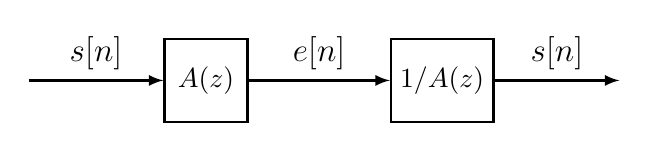
\begin{tikzpicture}[auto, thick, node distance=0.6cm, >=latex, scale = 0.75]
	\draw
	node at (2,0)[delay] (d1) {$A(z)$}
	node at (6,0) [delay] (p1) {$1/A(z)$};
	
	
	\draw[->](-1,0) -- node {\large$s[n]$}(d1);
	\draw[->](d1) -- node {\large$e[n]$} (p1);
	\draw[->](p1) -- node {\large$s[n]$} (9,0);


	
	\end{tikzpicture}
\end{center}
\end{frame}
\begin{frame}[fragile]
\vspace{0.5cm}
{\bfseries MATLAB Code Example} 
\begin{lstlisting}
[x,fs] = audioread('C6_2_y.wav');     
LENGTH = length(x);                          
n = 0:1/fs:(LENGTH - 1)/fs;   

subplot(3,1,1),plot(n*1000, x),grid 
xlabel('Time/s'); ylabel('Amplitude');
title('Original Signal')

subplot(3,1,2)
order = 20;
[a,g] = lpc(x,order);
error = filter(a,1,x);
plot(n*1000,error,'r')
xlabel('Time/s'); ylabel('Amplitude');
title('Predictive Error')

est_x = filter(1,a,error); 
subplot(3,1,3), plot(n*1000,est_x), grid;
xlabel('Time/s'); ylabel('Amplitude');
title('Predictive Signal')
\end{lstlisting}
\end{frame}
\begin{frame}
\vspace{0.5cm}
{\bfseries MATLAB Plot Example} 
% This file was created by matlab2tikz.
%
%The latest updates can be retrieved from
%  http://www.mathworks.com/matlabcentral/fileexchange/22022-matlab2tikz-matlab2tikz
%where you can also make suggestions and rate matlab2tikz.
%
\definecolor{mycolor1}{rgb}{0.00000,0.44700,0.74100}%
%
\begin{tikzpicture}[scale = 0.5]

\begin{axis}[%
width=6.275in,
height=0.899in,
at={(1.053in,3.809in)},
scale only axis,
xmin=0,
xmax=3500,
xlabel style={font=\color{white!15!black}},
xlabel={Time/s},
ymin=-1,
ymax=1,
ylabel style={font=\color{white!15!black}},
ylabel={Amplitude},
%axis background/.style={fill=white},
title style={font=\bfseries},
title={Original Signal},
xmajorgrids,
ymajorgrids
]
\addplot [color=mycolor1, forget plot]
  table[row sep=crcr]{%
0	-0.087432861328125\\
0.125	-0.087432861328125\\
0.25	-0.087432861328125\\
0.375	-0.0875244140625\\
0.5	-0.087615966796875\\
0.625	-0.087921142578125\\
0.75	-0.088958740234375\\
0.875	-0.059600830078125\\
1	-0.0601806640625\\
1.125	-0.060943603515625\\
1.25	-0.061279296875\\
1.375	-0.061370849609375\\
1.5	-0.061553955078125\\
1.625	-0.06158447265625\\
1.75	-0.06134033203125\\
1.875	-0.0616455078125\\
2	-0.06121826171875\\
2.125	-0.06207275390625\\
2.25	-0.06207275390625\\
2.375	-0.061981201171875\\
2.5	-0.0623779296875\\
2.625	-0.06170654296875\\
2.75	-0.062164306640625\\
2.875	-0.0618896484375\\
3	-0.0625\\
3.125	-0.0625\\
3.25	-0.0616455078125\\
3.375	-0.061553955078125\\
3.5	-0.062225341796875\\
3.625	-0.06231689453125\\
3.75	-0.06207275390625\\
3.875	-0.06231689453125\\
4	-0.06280517578125\\
4.125	-0.062744140625\\
4.25	-0.063018798828125\\
4.375	-0.063140869140625\\
4.5	-0.06280517578125\\
4.625	-0.062652587890625\\
4.75	-0.06317138671875\\
4.875	-0.063690185546875\\
5	-0.063323974609375\\
5.125	-0.064178466796875\\
5.25	-0.063690185546875\\
5.375	-0.0634765625\\
5.5	-0.064117431640625\\
5.625	-0.064483642578125\\
5.75	-0.064178466796875\\
5.875	-0.06427001953125\\
6	-0.06463623046875\\
6.125	-0.06451416015625\\
6.25	-0.06451416015625\\
6.375	-0.064605712890625\\
6.5	-0.06439208984375\\
6.625	-0.064300537109375\\
6.75	-0.065155029296875\\
6.875	-0.064727783203125\\
7	-0.064422607421875\\
7.125	-0.064727783203125\\
7.25	-0.064300537109375\\
7.375	-0.064056396484375\\
7.5	-0.06427001953125\\
7.625	-0.063995361328125\\
7.75	-0.0638427734375\\
7.875	-0.06378173828125\\
8	-0.064544677734375\\
8.125	-0.0640869140625\\
8.25	-0.06390380859375\\
8.375	-0.063751220703125\\
8.5	-0.06317138671875\\
8.625	-0.06353759765625\\
8.75	-0.064117431640625\\
8.875	-0.0638427734375\\
9	-0.06365966796875\\
9.125	-0.063751220703125\\
9.25	-0.063568115234375\\
9.375	-0.063568115234375\\
9.5	-0.063751220703125\\
9.625	-0.063446044921875\\
9.75	-0.063385009765625\\
9.875	-0.063323974609375\\
10	-0.0635986328125\\
10.125	-0.06317138671875\\
10.25	-0.063262939453125\\
10.375	-0.063323974609375\\
10.5	-0.06365966796875\\
10.625	-0.06292724609375\\
10.75	-0.062530517578125\\
10.875	-0.062408447265625\\
11	-0.0625\\
11.125	-0.062286376953125\\
11.25	-0.06170654296875\\
11.375	-0.06231689453125\\
11.5	-0.06231689453125\\
11.625	-0.06201171875\\
11.75	-0.06231689453125\\
11.875	-0.061981201171875\\
12	-0.061798095703125\\
12.125	-0.062225341796875\\
12.25	-0.062225341796875\\
12.375	-0.06243896484375\\
12.5	-0.062103271484375\\
12.625	-0.062286376953125\\
12.75	-0.06201171875\\
12.875	-0.06158447265625\\
13	-0.0618896484375\\
13.125	-0.06207275390625\\
13.25	-0.061981201171875\\
13.375	-0.062286376953125\\
13.5	-0.0623779296875\\
13.625	-0.062408447265625\\
13.75	-0.061676025390625\\
13.875	-0.061767578125\\
14	-0.061981201171875\\
14.125	-0.06146240234375\\
14.25	-0.061553955078125\\
14.375	-0.061676025390625\\
14.5	-0.06201171875\\
14.625	-0.06146240234375\\
14.75	-0.061767578125\\
14.875	-0.061431884765625\\
15	-0.06201171875\\
15.125	-0.061767578125\\
15.25	-0.061767578125\\
15.375	-0.06201171875\\
15.5	-0.06207275390625\\
15.625	-0.0618896484375\\
15.75	-0.062591552734375\\
15.875	-0.06231689453125\\
16	-0.062713623046875\\
16.125	-0.062713623046875\\
16.25	-0.0634765625\\
16.375	-0.063385009765625\\
16.5	-0.063018798828125\\
16.625	-0.062652587890625\\
16.75	-0.062896728515625\\
16.875	-0.062835693359375\\
17	-0.062164306640625\\
17.125	-0.0631103515625\\
17.25	-0.063323974609375\\
17.375	-0.063018798828125\\
17.5	-0.063262939453125\\
17.625	-0.06317138671875\\
17.75	-0.062896728515625\\
17.875	-0.063385009765625\\
18	-0.0631103515625\\
18.125	-0.062744140625\\
18.25	-0.0623779296875\\
18.375	-0.06207275390625\\
18.5	-0.06195068359375\\
18.625	-0.062286376953125\\
18.75	-0.062713623046875\\
18.875	-0.06231689453125\\
19	-0.063385009765625\\
19.125	-0.06243896484375\\
19.25	-0.06231689453125\\
19.375	-0.0625\\
19.5	-0.062530517578125\\
19.625	-0.062744140625\\
19.75	-0.062530517578125\\
19.875	-0.0626220703125\\
20	-0.062713623046875\\
20.125	-0.062530517578125\\
20.25	-0.06317138671875\\
20.375	-0.063140869140625\\
20.5	-0.062591552734375\\
20.625	-0.06317138671875\\
20.75	-0.062896728515625\\
20.875	-0.063262939453125\\
21	-0.063018798828125\\
21.125	-0.063446044921875\\
21.25	-0.063262939453125\\
21.375	-0.0633544921875\\
21.5	-0.063446044921875\\
21.625	-0.06280517578125\\
21.75	-0.0633544921875\\
21.875	-0.06317138671875\\
22	-0.062957763671875\\
22.125	-0.06292724609375\\
22.25	-0.063446044921875\\
22.375	-0.0635986328125\\
22.5	-0.063140869140625\\
22.625	-0.062835693359375\\
22.75	-0.063018798828125\\
22.875	-0.063385009765625\\
23	-0.063140869140625\\
23.125	-0.063232421875\\
23.25	-0.0631103515625\\
23.375	-0.062652587890625\\
23.5	-0.06280517578125\\
23.625	-0.06292724609375\\
23.75	-0.062835693359375\\
23.875	-0.062713623046875\\
24	-0.06201171875\\
24.125	-0.062103271484375\\
24.25	-0.061981201171875\\
24.375	-0.061798095703125\\
24.5	-0.062286376953125\\
24.625	-0.062408447265625\\
24.75	-0.06201171875\\
24.875	-0.061248779296875\\
25	-0.06121826171875\\
25.125	-0.06121826171875\\
25.25	-0.061065673828125\\
25.375	-0.06097412109375\\
25.5	-0.0609130859375\\
25.625	-0.06097412109375\\
25.75	-0.0611572265625\\
25.875	-0.060546875\\
26	-0.060699462890625\\
26.125	-0.06085205078125\\
26.25	-0.061248779296875\\
26.375	-0.061248779296875\\
26.5	-0.06060791015625\\
26.625	-0.060760498046875\\
26.75	-0.06072998046875\\
26.875	-0.060760498046875\\
27	-0.061370849609375\\
27.125	-0.06072998046875\\
27.25	-0.060821533203125\\
27.375	-0.06072998046875\\
27.5	-0.0601806640625\\
27.625	-0.06011962890625\\
27.75	-0.06011962890625\\
27.875	-0.05987548828125\\
28	-0.05987548828125\\
28.125	-0.05975341796875\\
28.25	-0.05938720703125\\
28.375	-0.05938720703125\\
28.5	-0.059814453125\\
28.625	-0.058746337890625\\
28.75	-0.059600830078125\\
28.875	-0.0595703125\\
29	-0.059478759765625\\
29.125	-0.059661865234375\\
29.25	-0.059661865234375\\
29.375	-0.060089111328125\\
29.5	-0.060394287109375\\
29.625	-0.06011962890625\\
29.75	-0.05999755859375\\
29.875	-0.059967041015625\\
30	-0.060089111328125\\
30.125	-0.05987548828125\\
30.25	-0.059539794921875\\
30.375	-0.05975341796875\\
30.5	-0.059600830078125\\
30.625	-0.059478759765625\\
30.75	-0.059600830078125\\
30.875	-0.05987548828125\\
31	-0.05999755859375\\
31.125	-0.059906005859375\\
31.25	-0.05987548828125\\
31.375	-0.0595703125\\
31.5	-0.060211181640625\\
31.625	-0.0604248046875\\
31.75	-0.05999755859375\\
31.875	-0.060333251953125\\
32	-0.060333251953125\\
32.125	-0.0604248046875\\
32.25	-0.059783935546875\\
32.375	-0.06072998046875\\
32.5	-0.0604248046875\\
32.625	-0.05975341796875\\
32.75	-0.060516357421875\\
32.875	-0.0611572265625\\
33	-0.06048583984375\\
33.125	-0.0601806640625\\
33.25	-0.06060791015625\\
33.375	-0.060821533203125\\
33.5	-0.060394287109375\\
33.625	-0.06097412109375\\
33.75	-0.06103515625\\
33.875	-0.060760498046875\\
34	-0.060516357421875\\
34.125	-0.060394287109375\\
34.25	-0.060546875\\
34.375	-0.060302734375\\
34.5	-0.060302734375\\
34.625	-0.060272216796875\\
34.75	-0.06011962890625\\
34.875	-0.060333251953125\\
35	-0.060028076171875\\
35.125	-0.060333251953125\\
35.25	-0.060394287109375\\
35.375	-0.060638427734375\\
35.5	-0.06121826171875\\
35.625	-0.060760498046875\\
35.75	-0.0611572265625\\
35.875	-0.060699462890625\\
36	-0.060943603515625\\
36.125	-0.060760498046875\\
36.25	-0.061126708984375\\
36.375	-0.060821533203125\\
36.5	-0.06072998046875\\
36.625	-0.061065673828125\\
36.75	-0.06097412109375\\
36.875	-0.061492919921875\\
37	-0.06072998046875\\
37.125	-0.06158447265625\\
37.25	-0.061065673828125\\
37.375	-0.060516357421875\\
37.5	-0.06170654296875\\
37.625	-0.061370849609375\\
37.75	-0.06085205078125\\
37.875	-0.061279296875\\
38	-0.061676025390625\\
38.125	-0.06146240234375\\
38.25	-0.060760498046875\\
38.375	-0.0611572265625\\
38.5	-0.06103515625\\
38.625	-0.061370849609375\\
38.75	-0.06085205078125\\
38.875	-0.06134033203125\\
39	-0.06121826171875\\
39.125	-0.061370849609375\\
39.25	-0.0611572265625\\
39.375	-0.061492919921875\\
39.5	-0.061553955078125\\
39.625	-0.06121826171875\\
39.75	-0.061370849609375\\
39.875	-0.061767578125\\
40	-0.06103515625\\
40.125	-0.060943603515625\\
40.25	-0.0609130859375\\
40.375	-0.060638427734375\\
40.5	-0.060821533203125\\
40.625	-0.06072998046875\\
40.75	-0.0604248046875\\
40.875	-0.060699462890625\\
41	-0.0601806640625\\
41.125	-0.060394287109375\\
41.25	-0.06060791015625\\
41.375	-0.06011962890625\\
41.5	-0.059814453125\\
41.625	-0.0595703125\\
41.75	-0.059478759765625\\
41.875	-0.060089111328125\\
42	-0.059906005859375\\
42.125	-0.05975341796875\\
42.25	-0.06011962890625\\
42.375	-0.059539794921875\\
42.5	-0.060302734375\\
42.625	-0.0596923828125\\
42.75	-0.059814453125\\
42.875	-0.060028076171875\\
43	-0.06011962890625\\
43.125	-0.05987548828125\\
43.25	-0.059600830078125\\
43.375	-0.060272216796875\\
43.5	-0.06011962890625\\
43.625	-0.060211181640625\\
43.75	-0.059967041015625\\
43.875	-0.06011962890625\\
44	-0.0604248046875\\
44.125	-0.05975341796875\\
44.25	-0.06011962890625\\
44.375	-0.059783935546875\\
44.5	-0.0595703125\\
44.625	-0.0595703125\\
44.75	-0.059051513671875\\
44.875	-0.0596923828125\\
45	-0.05999755859375\\
45.125	-0.05987548828125\\
45.25	-0.059478759765625\\
45.375	-0.060394287109375\\
45.5	-0.059783935546875\\
45.625	-0.060028076171875\\
45.75	-0.060516357421875\\
45.875	-0.060546875\\
46	-0.06011962890625\\
46.125	-0.060760498046875\\
46.25	-0.060638427734375\\
46.375	-0.06072998046875\\
46.5	-0.060821533203125\\
46.625	-0.061370849609375\\
46.75	-0.06085205078125\\
46.875	-0.061370849609375\\
47	-0.060333251953125\\
47.125	-0.060546875\\
47.25	-0.0604248046875\\
47.375	-0.060089111328125\\
47.5	-0.060302734375\\
47.625	-0.061248779296875\\
47.75	-0.060821533203125\\
47.875	-0.060699462890625\\
48	-0.06085205078125\\
48.125	-0.060638427734375\\
48.25	-0.060638427734375\\
48.375	-0.06103515625\\
48.5	-0.06072998046875\\
48.625	-0.060943603515625\\
48.75	-0.060821533203125\\
48.875	-0.061248779296875\\
49	-0.06146240234375\\
49.125	-0.061767578125\\
49.25	-0.061248779296875\\
49.375	-0.061492919921875\\
49.5	-0.06170654296875\\
49.625	-0.06243896484375\\
49.75	-0.061798095703125\\
49.875	-0.0623779296875\\
50	-0.0623779296875\\
50.125	-0.062652587890625\\
50.25	-0.063232421875\\
50.375	-0.063568115234375\\
50.5	-0.062744140625\\
50.625	-0.062591552734375\\
50.75	-0.062713623046875\\
50.875	-0.06353759765625\\
51	-0.063385009765625\\
51.125	-0.063568115234375\\
51.25	-0.0640869140625\\
51.375	-0.063385009765625\\
51.5	-0.06390380859375\\
51.625	-0.063568115234375\\
51.75	-0.06378173828125\\
51.875	-0.063446044921875\\
52	-0.063873291015625\\
52.125	-0.063568115234375\\
52.25	-0.064422607421875\\
52.375	-0.06427001953125\\
52.5	-0.064208984375\\
52.625	-0.0638427734375\\
52.75	-0.064178466796875\\
52.875	-0.06378173828125\\
53	-0.063995361328125\\
53.125	-0.064208984375\\
53.25	-0.064788818359375\\
53.375	-0.064483642578125\\
53.5	-0.064605712890625\\
53.625	-0.064117431640625\\
53.75	-0.0643310546875\\
53.875	-0.064208984375\\
54	-0.06451416015625\\
54.125	-0.06427001953125\\
54.25	-0.06396484375\\
54.375	-0.064697265625\\
54.5	-0.064849853515625\\
54.625	-0.064300537109375\\
54.75	-0.06451416015625\\
54.875	-0.06439208984375\\
55	-0.064117431640625\\
55.125	-0.06439208984375\\
55.25	-0.063568115234375\\
55.375	-0.06396484375\\
55.5	-0.063995361328125\\
55.625	-0.064422607421875\\
55.75	-0.06439208984375\\
55.875	-0.064483642578125\\
56	-0.0643310546875\\
56.125	-0.064544677734375\\
56.25	-0.064178466796875\\
56.375	-0.063995361328125\\
56.5	-0.064697265625\\
56.625	-0.064208984375\\
56.75	-0.06463623046875\\
56.875	-0.0640869140625\\
57	-0.064300537109375\\
57.125	-0.064056396484375\\
57.25	-0.06365966796875\\
57.375	-0.06390380859375\\
57.5	-0.0633544921875\\
57.625	-0.063568115234375\\
57.75	-0.0635986328125\\
57.875	-0.063385009765625\\
58	-0.06378173828125\\
58.125	-0.0635986328125\\
58.25	-0.063385009765625\\
58.375	-0.0631103515625\\
58.5	-0.062896728515625\\
58.625	-0.062957763671875\\
58.75	-0.063385009765625\\
58.875	-0.06231689453125\\
59	-0.062591552734375\\
59.125	-0.062957763671875\\
59.25	-0.062408447265625\\
59.375	-0.0626220703125\\
59.5	-0.062896728515625\\
59.625	-0.0623779296875\\
59.75	-0.062286376953125\\
59.875	-0.062530517578125\\
60	-0.0623779296875\\
60.125	-0.062652587890625\\
60.25	-0.062103271484375\\
60.375	-0.0625\\
60.5	-0.06207275390625\\
60.625	-0.062103271484375\\
60.75	-0.062164306640625\\
60.875	-0.06195068359375\\
61	-0.061676025390625\\
61.125	-0.06146240234375\\
61.25	-0.06146240234375\\
61.375	-0.061065673828125\\
61.5	-0.06146240234375\\
61.625	-0.061248779296875\\
61.75	-0.06085205078125\\
61.875	-0.061676025390625\\
62	-0.061676025390625\\
62.125	-0.06146240234375\\
62.25	-0.061370849609375\\
62.375	-0.0616455078125\\
62.5	-0.061553955078125\\
62.625	-0.061492919921875\\
62.75	-0.06158447265625\\
62.875	-0.06231689453125\\
63	-0.061065673828125\\
63.125	-0.06170654296875\\
63.25	-0.06158447265625\\
63.375	-0.0618896484375\\
63.5	-0.061553955078125\\
63.625	-0.06146240234375\\
63.75	-0.0616455078125\\
63.875	-0.06072998046875\\
64	-0.061279296875\\
64.125	-0.061553955078125\\
64.25	-0.06158447265625\\
64.375	-0.0616455078125\\
64.5	-0.06097412109375\\
64.625	-0.06158447265625\\
64.75	-0.06170654296875\\
64.875	-0.0616455078125\\
65	-0.061248779296875\\
65.125	-0.061279296875\\
65.25	-0.061065673828125\\
65.375	-0.06231689453125\\
65.5	-0.061248779296875\\
65.625	-0.06146240234375\\
65.75	-0.06201171875\\
65.875	-0.06146240234375\\
66	-0.0616455078125\\
66.125	-0.0625\\
66.25	-0.06219482421875\\
66.375	-0.06243896484375\\
66.5	-0.06231689453125\\
66.625	-0.06280517578125\\
66.75	-0.06231689453125\\
66.875	-0.062835693359375\\
67	-0.062896728515625\\
67.125	-0.06292724609375\\
67.25	-0.0623779296875\\
67.375	-0.062286376953125\\
67.5	-0.062957763671875\\
67.625	-0.06280517578125\\
67.75	-0.062652587890625\\
67.875	-0.0626220703125\\
68	-0.0633544921875\\
68.125	-0.062744140625\\
68.25	-0.0635986328125\\
68.375	-0.063446044921875\\
68.5	-0.06304931640625\\
68.625	-0.06280517578125\\
68.75	-0.0631103515625\\
68.875	-0.063018798828125\\
69	-0.0638427734375\\
69.125	-0.06378173828125\\
69.25	-0.06390380859375\\
69.375	-0.063385009765625\\
69.5	-0.063385009765625\\
69.625	-0.063323974609375\\
69.75	-0.06365966796875\\
69.875	-0.063690185546875\\
70	-0.06304931640625\\
70.125	-0.0635986328125\\
70.25	-0.063751220703125\\
70.375	-0.0634765625\\
70.5	-0.062896728515625\\
70.625	-0.063140869140625\\
70.75	-0.063568115234375\\
70.875	-0.06353759765625\\
71	-0.062896728515625\\
71.125	-0.063751220703125\\
71.25	-0.063446044921875\\
71.375	-0.06396484375\\
71.5	-0.063446044921875\\
71.625	-0.063751220703125\\
71.75	-0.06378173828125\\
71.875	-0.063568115234375\\
72	-0.06427001953125\\
72.125	-0.0643310546875\\
72.25	-0.06390380859375\\
72.375	-0.064483642578125\\
72.5	-0.0638427734375\\
72.625	-0.06378173828125\\
72.75	-0.06427001953125\\
72.875	-0.064178466796875\\
73	-0.06378173828125\\
73.125	-0.0634765625\\
73.25	-0.06353759765625\\
73.375	-0.063140869140625\\
73.5	-0.06317138671875\\
73.625	-0.063140869140625\\
73.75	-0.062957763671875\\
73.875	-0.0633544921875\\
74	-0.062835693359375\\
74.125	-0.062713623046875\\
74.25	-0.062225341796875\\
74.375	-0.061767578125\\
74.5	-0.06195068359375\\
74.625	-0.062103271484375\\
74.75	-0.06219482421875\\
74.875	-0.06170654296875\\
75	-0.061767578125\\
75.125	-0.06146240234375\\
75.25	-0.061492919921875\\
75.375	-0.06085205078125\\
75.5	-0.061279296875\\
75.625	-0.060821533203125\\
75.75	-0.06072998046875\\
75.875	-0.060760498046875\\
76	-0.06060791015625\\
76.125	-0.060760498046875\\
76.25	-0.060302734375\\
76.375	-0.060028076171875\\
76.5	-0.06048583984375\\
76.625	-0.060211181640625\\
76.75	-0.0595703125\\
76.875	-0.05987548828125\\
77	-0.05987548828125\\
77.125	-0.060028076171875\\
77.25	-0.059539794921875\\
77.375	-0.058807373046875\\
77.5	-0.058868408203125\\
77.625	-0.059051513671875\\
77.75	-0.059478759765625\\
77.875	-0.058746337890625\\
78	-0.059051513671875\\
78.125	-0.058929443359375\\
78.25	-0.059234619140625\\
78.375	-0.058929443359375\\
78.5	-0.059234619140625\\
78.625	-0.059356689453125\\
78.75	-0.059600830078125\\
78.875	-0.0595703125\\
79	-0.059356689453125\\
79.125	-0.05908203125\\
79.25	-0.059326171875\\
79.375	-0.05926513671875\\
79.5	-0.059783935546875\\
79.625	-0.0594482421875\\
79.75	-0.060089111328125\\
79.875	-0.060028076171875\\
80	-0.059967041015625\\
80.125	-0.060272216796875\\
80.25	-0.06072998046875\\
80.375	-0.05999755859375\\
80.5	-0.060272216796875\\
80.625	-0.05975341796875\\
80.75	-0.060028076171875\\
80.875	-0.060699462890625\\
81	-0.060333251953125\\
81.125	-0.060272216796875\\
81.25	-0.060333251953125\\
81.375	-0.06048583984375\\
81.5	-0.060516357421875\\
81.625	-0.060211181640625\\
81.75	-0.060760498046875\\
81.875	-0.06072998046875\\
82	-0.060699462890625\\
82.125	-0.060333251953125\\
82.25	-0.060943603515625\\
82.375	-0.060760498046875\\
82.5	-0.06072998046875\\
82.625	-0.0609130859375\\
82.75	-0.061553955078125\\
82.875	-0.06207275390625\\
83	-0.061798095703125\\
83.125	-0.06158447265625\\
83.25	-0.062103271484375\\
83.375	-0.06195068359375\\
83.5	-0.06219482421875\\
83.625	-0.06195068359375\\
83.75	-0.0623779296875\\
83.875	-0.062103271484375\\
84	-0.061798095703125\\
84.125	-0.062896728515625\\
84.25	-0.062408447265625\\
84.375	-0.061981201171875\\
84.5	-0.062408447265625\\
84.625	-0.06231689453125\\
84.75	-0.062103271484375\\
84.875	-0.061981201171875\\
85	-0.062225341796875\\
85.125	-0.062286376953125\\
85.25	-0.062652587890625\\
85.375	-0.062408447265625\\
85.5	-0.062744140625\\
85.625	-0.062957763671875\\
85.75	-0.063018798828125\\
85.875	-0.06280517578125\\
86	-0.06243896484375\\
86.125	-0.062835693359375\\
86.25	-0.06292724609375\\
86.375	-0.0623779296875\\
86.5	-0.062957763671875\\
86.625	-0.063018798828125\\
86.75	-0.063385009765625\\
86.875	-0.063323974609375\\
87	-0.062530517578125\\
87.125	-0.063018798828125\\
87.25	-0.063262939453125\\
87.375	-0.0633544921875\\
87.5	-0.063385009765625\\
87.625	-0.063568115234375\\
87.75	-0.063018798828125\\
87.875	-0.062957763671875\\
88	-0.06304931640625\\
88.125	-0.06317138671875\\
88.25	-0.062744140625\\
88.375	-0.062896728515625\\
88.5	-0.062408447265625\\
88.625	-0.062225341796875\\
88.75	-0.062713623046875\\
88.875	-0.06280517578125\\
89	-0.062652587890625\\
89.125	-0.062530517578125\\
89.25	-0.062164306640625\\
89.375	-0.063232421875\\
89.5	-0.063018798828125\\
89.625	-0.062164306640625\\
89.75	-0.06201171875\\
89.875	-0.062408447265625\\
90	-0.06243896484375\\
90.125	-0.062164306640625\\
90.25	-0.062286376953125\\
90.375	-0.06201171875\\
90.5	-0.06146240234375\\
90.625	-0.06097412109375\\
90.75	-0.061676025390625\\
90.875	-0.061431884765625\\
91	-0.061248779296875\\
91.125	-0.061065673828125\\
91.25	-0.0616455078125\\
91.375	-0.06121826171875\\
91.5	-0.061126708984375\\
91.625	-0.060516357421875\\
91.75	-0.0604248046875\\
91.875	-0.06011962890625\\
92	-0.05999755859375\\
92.125	-0.05999755859375\\
92.25	-0.0601806640625\\
92.375	-0.060272216796875\\
92.5	-0.060211181640625\\
92.625	-0.060211181640625\\
92.75	-0.060089111328125\\
92.875	-0.05987548828125\\
93	-0.059478759765625\\
93.125	-0.059967041015625\\
93.25	-0.059906005859375\\
93.375	-0.05999755859375\\
93.5	-0.05987548828125\\
93.625	-0.059814453125\\
93.75	-0.05975341796875\\
93.875	-0.060028076171875\\
94	-0.059234619140625\\
94.125	-0.05926513671875\\
94.25	-0.0594482421875\\
94.375	-0.0595703125\\
94.5	-0.059326171875\\
94.625	-0.059051513671875\\
94.75	-0.059326171875\\
94.875	-0.059173583984375\\
95	-0.05938720703125\\
95.125	-0.05938720703125\\
95.25	-0.05902099609375\\
95.375	-0.05926513671875\\
95.5	-0.05938720703125\\
95.625	-0.058868408203125\\
95.75	-0.0594482421875\\
95.875	-0.0595703125\\
96	-0.05926513671875\\
96.125	-0.060333251953125\\
96.25	-0.060333251953125\\
96.375	-0.059814453125\\
96.5	-0.05975341796875\\
96.625	-0.060302734375\\
96.75	-0.059967041015625\\
96.875	-0.059967041015625\\
97	-0.060333251953125\\
97.125	-0.0596923828125\\
97.25	-0.0596923828125\\
97.375	-0.05999755859375\\
97.5	-0.060028076171875\\
97.625	-0.060089111328125\\
97.75	-0.0596923828125\\
97.875	-0.060516357421875\\
98	-0.06048583984375\\
98.125	-0.0601806640625\\
98.25	-0.060089111328125\\
98.375	-0.06011962890625\\
98.5	-0.059783935546875\\
98.625	-0.06072998046875\\
98.75	-0.060760498046875\\
98.875	-0.06072998046875\\
99	-0.0611572265625\\
99.125	-0.060821533203125\\
99.25	-0.060699462890625\\
99.375	-0.061279296875\\
99.5	-0.061126708984375\\
99.625	-0.0611572265625\\
99.75	-0.060943603515625\\
99.875	-0.0611572265625\\
100	-0.06121826171875\\
100.125	-0.061279296875\\
100.25	-0.06201171875\\
100.375	-0.061798095703125\\
100.5	-0.061767578125\\
100.625	-0.0618896484375\\
100.75	-0.0618896484375\\
100.875	-0.061798095703125\\
101	-0.0623779296875\\
101.125	-0.06201171875\\
101.25	-0.062408447265625\\
101.375	-0.06219482421875\\
101.5	-0.06207275390625\\
101.625	-0.06207275390625\\
101.75	-0.061676025390625\\
101.875	-0.062164306640625\\
102	-0.062103271484375\\
102.125	-0.0623779296875\\
102.25	-0.0626220703125\\
102.375	-0.062286376953125\\
102.5	-0.06219482421875\\
102.625	-0.062164306640625\\
102.75	-0.06219482421875\\
102.875	-0.06243896484375\\
103	-0.0625\\
103.125	-0.062408447265625\\
103.25	-0.062957763671875\\
103.375	-0.062835693359375\\
103.5	-0.063018798828125\\
103.625	-0.062896728515625\\
103.75	-0.062225341796875\\
103.875	-0.06243896484375\\
104	-0.06280517578125\\
104.125	-0.063262939453125\\
104.25	-0.06317138671875\\
104.375	-0.063446044921875\\
104.5	-0.062957763671875\\
104.625	-0.063873291015625\\
104.75	-0.063446044921875\\
104.875	-0.06304931640625\\
105	-0.063323974609375\\
105.125	-0.06280517578125\\
105.25	-0.062835693359375\\
105.375	-0.062957763671875\\
105.5	-0.063262939453125\\
105.625	-0.063446044921875\\
105.75	-0.063140869140625\\
105.875	-0.063262939453125\\
106	-0.063140869140625\\
106.125	-0.0631103515625\\
106.25	-0.063140869140625\\
106.375	-0.063262939453125\\
106.5	-0.063232421875\\
106.625	-0.063446044921875\\
106.75	-0.063262939453125\\
106.875	-0.0633544921875\\
107	-0.0631103515625\\
107.125	-0.0625\\
107.25	-0.063262939453125\\
107.375	-0.062591552734375\\
107.5	-0.062744140625\\
107.625	-0.062835693359375\\
107.75	-0.06304931640625\\
107.875	-0.062652587890625\\
108	-0.062835693359375\\
108.125	-0.06304931640625\\
108.25	-0.062591552734375\\
108.375	-0.0625\\
108.5	-0.062652587890625\\
108.625	-0.0623779296875\\
108.75	-0.06317138671875\\
108.875	-0.062957763671875\\
109	-0.062957763671875\\
109.125	-0.06317138671875\\
109.25	-0.063323974609375\\
109.375	-0.0635986328125\\
109.5	-0.06304931640625\\
109.625	-0.0631103515625\\
109.75	-0.062896728515625\\
109.875	-0.0634765625\\
110	-0.063323974609375\\
110.125	-0.062957763671875\\
110.25	-0.063018798828125\\
110.375	-0.06304931640625\\
110.5	-0.06292724609375\\
110.625	-0.06304931640625\\
110.75	-0.062225341796875\\
110.875	-0.06207275390625\\
111	-0.061553955078125\\
111.125	-0.06158447265625\\
111.25	-0.06103515625\\
111.375	-0.06134033203125\\
111.5	-0.06170654296875\\
111.625	-0.061126708984375\\
111.75	-0.0616455078125\\
111.875	-0.060699462890625\\
112	-0.06097412109375\\
112.125	-0.06072998046875\\
112.25	-0.060333251953125\\
112.375	-0.060821533203125\\
112.5	-0.06146240234375\\
112.625	-0.061248779296875\\
112.75	-0.060943603515625\\
112.875	-0.06121826171875\\
113	-0.061065673828125\\
113.125	-0.060943603515625\\
113.25	-0.061065673828125\\
113.375	-0.060699462890625\\
113.5	-0.061126708984375\\
113.625	-0.06103515625\\
113.75	-0.06085205078125\\
113.875	-0.060638427734375\\
114	-0.06103515625\\
114.125	-0.060699462890625\\
114.25	-0.06085205078125\\
114.375	-0.060821533203125\\
114.5	-0.06060791015625\\
114.625	-0.0611572265625\\
114.75	-0.06121826171875\\
114.875	-0.061248779296875\\
115	-0.061065673828125\\
115.125	-0.06060791015625\\
115.25	-0.06048583984375\\
115.375	-0.060821533203125\\
115.5	-0.061553955078125\\
115.625	-0.060760498046875\\
115.75	-0.06072998046875\\
115.875	-0.06085205078125\\
116	-0.06072998046875\\
116.125	-0.06103515625\\
116.25	-0.061065673828125\\
116.375	-0.06097412109375\\
116.5	-0.060821533203125\\
116.625	-0.061492919921875\\
116.75	-0.06146240234375\\
116.875	-0.06103515625\\
117	-0.06121826171875\\
117.125	-0.061431884765625\\
117.25	-0.06085205078125\\
117.375	-0.061370849609375\\
117.5	-0.06146240234375\\
117.625	-0.061553955078125\\
117.75	-0.0616455078125\\
117.875	-0.060943603515625\\
118	-0.061676025390625\\
118.125	-0.06103515625\\
118.25	-0.061126708984375\\
118.375	-0.06158447265625\\
118.5	-0.061279296875\\
118.625	-0.06146240234375\\
118.75	-0.06158447265625\\
118.875	-0.061553955078125\\
119	-0.062103271484375\\
119.125	-0.061859130859375\\
119.25	-0.061767578125\\
119.375	-0.06195068359375\\
119.5	-0.061126708984375\\
119.625	-0.06195068359375\\
119.75	-0.06195068359375\\
119.875	-0.06103515625\\
120	-0.06207275390625\\
120.125	-0.06195068359375\\
120.25	-0.061859130859375\\
120.375	-0.061981201171875\\
120.5	-0.06201171875\\
120.625	-0.06170654296875\\
120.75	-0.062408447265625\\
120.875	-0.0625\\
121	-0.06207275390625\\
121.125	-0.0626220703125\\
121.25	-0.062103271484375\\
121.375	-0.062530517578125\\
121.5	-0.06207275390625\\
121.625	-0.062103271484375\\
121.75	-0.062103271484375\\
121.875	-0.062591552734375\\
122	-0.062652587890625\\
122.125	-0.0623779296875\\
122.25	-0.062103271484375\\
122.375	-0.06304931640625\\
122.5	-0.062957763671875\\
122.625	-0.062957763671875\\
122.75	-0.06207275390625\\
122.875	-0.06243896484375\\
123	-0.062713623046875\\
123.125	-0.062408447265625\\
123.25	-0.062744140625\\
123.375	-0.062164306640625\\
123.5	-0.06195068359375\\
123.625	-0.06195068359375\\
123.75	-0.06158447265625\\
123.875	-0.06195068359375\\
124	-0.061553955078125\\
124.125	-0.06121826171875\\
124.25	-0.06146240234375\\
124.375	-0.061492919921875\\
124.5	-0.061981201171875\\
124.625	-0.06121826171875\\
124.75	-0.061370849609375\\
124.875	-0.06146240234375\\
125	-0.061767578125\\
125.125	-0.062103271484375\\
125.25	-0.061798095703125\\
125.375	-0.06158447265625\\
125.5	-0.061553955078125\\
125.625	-0.061981201171875\\
125.75	-0.061676025390625\\
125.875	-0.0618896484375\\
126	-0.06219482421875\\
126.125	-0.061676025390625\\
126.25	-0.06207275390625\\
126.375	-0.061859130859375\\
126.5	-0.062408447265625\\
126.625	-0.06201171875\\
126.75	-0.062530517578125\\
126.875	-0.06170654296875\\
127	-0.06243896484375\\
127.125	-0.06207275390625\\
127.25	-0.06170654296875\\
127.375	-0.060821533203125\\
127.5	-0.06207275390625\\
127.625	-0.061279296875\\
127.75	-0.061279296875\\
127.875	-0.06170654296875\\
128	-0.061279296875\\
128.125	-0.06146240234375\\
128.25	-0.060760498046875\\
128.375	-0.0609130859375\\
128.5	-0.061553955078125\\
128.625	-0.061431884765625\\
128.75	-0.061126708984375\\
128.875	-0.06085205078125\\
129	-0.0609130859375\\
129.125	-0.060638427734375\\
129.25	-0.060333251953125\\
129.375	-0.060333251953125\\
129.5	-0.06103515625\\
129.625	-0.06011962890625\\
129.75	-0.060302734375\\
129.875	-0.06048583984375\\
130	-0.060394287109375\\
130.125	-0.060333251953125\\
130.25	-0.060333251953125\\
130.375	-0.060089111328125\\
130.5	-0.059783935546875\\
130.625	-0.059661865234375\\
130.75	-0.059906005859375\\
130.875	-0.059814453125\\
131	-0.059967041015625\\
131.125	-0.06011962890625\\
131.25	-0.059539794921875\\
131.375	-0.0594482421875\\
131.5	-0.0595703125\\
131.625	-0.059661865234375\\
131.75	-0.05987548828125\\
131.875	-0.059783935546875\\
132	-0.059600830078125\\
132.125	-0.059539794921875\\
132.25	-0.05938720703125\\
132.375	-0.059478759765625\\
132.5	-0.05975341796875\\
132.625	-0.060028076171875\\
132.75	-0.059783935546875\\
132.875	-0.060546875\\
133	-0.059906005859375\\
133.125	-0.05987548828125\\
133.25	-0.059783935546875\\
133.375	-0.060089111328125\\
133.5	-0.060516357421875\\
133.625	-0.060272216796875\\
133.75	-0.060394287109375\\
133.875	-0.060638427734375\\
134	-0.06011962890625\\
134.125	-0.06072998046875\\
134.25	-0.060699462890625\\
134.375	-0.060943603515625\\
134.5	-0.0616455078125\\
134.625	-0.06170654296875\\
134.75	-0.061676025390625\\
134.875	-0.06158447265625\\
135	-0.061676025390625\\
135.125	-0.061981201171875\\
135.25	-0.062103271484375\\
135.375	-0.06201171875\\
135.5	-0.06195068359375\\
135.625	-0.062164306640625\\
135.75	-0.062530517578125\\
135.875	-0.06219482421875\\
136	-0.0618896484375\\
136.125	-0.062164306640625\\
136.25	-0.061676025390625\\
136.375	-0.06201171875\\
136.5	-0.06201171875\\
136.625	-0.0618896484375\\
136.75	-0.061859130859375\\
136.875	-0.0618896484375\\
137	-0.061798095703125\\
137.125	-0.062164306640625\\
137.25	-0.0626220703125\\
137.375	-0.062957763671875\\
137.5	-0.062896728515625\\
137.625	-0.063018798828125\\
137.75	-0.06317138671875\\
137.875	-0.062591552734375\\
138	-0.062835693359375\\
138.125	-0.062896728515625\\
138.25	-0.062835693359375\\
138.375	-0.062896728515625\\
138.5	-0.0633544921875\\
138.625	-0.0634765625\\
138.75	-0.063751220703125\\
138.875	-0.063690185546875\\
139	-0.0640869140625\\
139.125	-0.064483642578125\\
139.25	-0.063568115234375\\
139.375	-0.063873291015625\\
139.5	-0.0635986328125\\
139.625	-0.063873291015625\\
139.75	-0.06427001953125\\
139.875	-0.0648193359375\\
140	-0.06396484375\\
140.125	-0.064117431640625\\
140.25	-0.06396484375\\
140.375	-0.063995361328125\\
140.5	-0.063568115234375\\
140.625	-0.06378173828125\\
140.75	-0.063751220703125\\
140.875	-0.063140869140625\\
141	-0.06292724609375\\
141.125	-0.063323974609375\\
141.25	-0.063751220703125\\
141.375	-0.063232421875\\
141.5	-0.062957763671875\\
141.625	-0.06292724609375\\
141.75	-0.063232421875\\
141.875	-0.062591552734375\\
142	-0.06280517578125\\
142.125	-0.062530517578125\\
142.25	-0.06243896484375\\
142.375	-0.063018798828125\\
142.5	-0.0625\\
142.625	-0.062835693359375\\
142.75	-0.06304931640625\\
142.875	-0.062530517578125\\
143	-0.06292724609375\\
143.125	-0.063018798828125\\
143.25	-0.062652587890625\\
143.375	-0.062896728515625\\
143.5	-0.062530517578125\\
143.625	-0.0625\\
143.75	-0.0626220703125\\
143.875	-0.062408447265625\\
144	-0.06243896484375\\
144.125	-0.062408447265625\\
144.25	-0.06207275390625\\
144.375	-0.06195068359375\\
144.5	-0.062225341796875\\
144.625	-0.062103271484375\\
144.75	-0.06195068359375\\
144.875	-0.061767578125\\
145	-0.062164306640625\\
145.125	-0.06146240234375\\
145.25	-0.061798095703125\\
145.375	-0.0618896484375\\
145.5	-0.062286376953125\\
145.625	-0.06219482421875\\
145.75	-0.06170654296875\\
145.875	-0.061981201171875\\
146	-0.061981201171875\\
146.125	-0.06231689453125\\
146.25	-0.06231689453125\\
146.375	-0.06243896484375\\
146.5	-0.06207275390625\\
146.625	-0.0626220703125\\
146.75	-0.063018798828125\\
146.875	-0.0625\\
147	-0.06207275390625\\
147.125	-0.061981201171875\\
147.25	-0.0618896484375\\
147.375	-0.062225341796875\\
147.5	-0.062103271484375\\
147.625	-0.062408447265625\\
147.75	-0.06243896484375\\
147.875	-0.061981201171875\\
148	-0.062286376953125\\
148.125	-0.06207275390625\\
148.25	-0.0623779296875\\
148.375	-0.06280517578125\\
148.5	-0.0623779296875\\
148.625	-0.06231689453125\\
148.75	-0.06207275390625\\
148.875	-0.062286376953125\\
149	-0.062164306640625\\
149.125	-0.062530517578125\\
149.25	-0.062713623046875\\
149.375	-0.06304931640625\\
149.5	-0.063262939453125\\
149.625	-0.062835693359375\\
149.75	-0.063140869140625\\
149.875	-0.0631103515625\\
150	-0.063262939453125\\
150.125	-0.063446044921875\\
150.25	-0.0631103515625\\
150.375	-0.06317138671875\\
150.5	-0.06378173828125\\
150.625	-0.0634765625\\
150.75	-0.063262939453125\\
150.875	-0.063690185546875\\
151	-0.063690185546875\\
151.125	-0.0635986328125\\
151.25	-0.062896728515625\\
151.375	-0.0634765625\\
151.5	-0.063568115234375\\
151.625	-0.063568115234375\\
151.75	-0.0633544921875\\
151.875	-0.063262939453125\\
152	-0.062530517578125\\
152.125	-0.06304931640625\\
152.25	-0.063751220703125\\
152.375	-0.06396484375\\
152.5	-0.063262939453125\\
152.625	-0.063140869140625\\
152.75	-0.06365966796875\\
152.875	-0.063690185546875\\
153	-0.063323974609375\\
153.125	-0.063446044921875\\
153.25	-0.063568115234375\\
153.375	-0.063323974609375\\
153.5	-0.0635986328125\\
153.625	-0.0638427734375\\
153.75	-0.063995361328125\\
153.875	-0.0638427734375\\
154	-0.0635986328125\\
154.125	-0.0638427734375\\
154.25	-0.06378173828125\\
154.375	-0.0635986328125\\
154.5	-0.063385009765625\\
154.625	-0.06353759765625\\
154.75	-0.0640869140625\\
154.875	-0.063873291015625\\
155	-0.0640869140625\\
155.125	-0.063690185546875\\
155.25	-0.06365966796875\\
155.375	-0.063385009765625\\
155.5	-0.06365966796875\\
155.625	-0.063873291015625\\
155.75	-0.0638427734375\\
155.875	-0.063446044921875\\
156	-0.064178466796875\\
156.125	-0.062652587890625\\
156.25	-0.063446044921875\\
156.375	-0.063140869140625\\
156.5	-0.06317138671875\\
156.625	-0.063262939453125\\
156.75	-0.062591552734375\\
156.875	-0.063018798828125\\
157	-0.062744140625\\
157.125	-0.06292724609375\\
157.25	-0.062408447265625\\
157.375	-0.062103271484375\\
157.5	-0.062896728515625\\
157.625	-0.06201171875\\
157.75	-0.06231689453125\\
157.875	-0.06219482421875\\
158	-0.061981201171875\\
158.125	-0.061279296875\\
158.25	-0.061798095703125\\
158.375	-0.061370849609375\\
158.5	-0.060760498046875\\
158.625	-0.06097412109375\\
158.75	-0.06103515625\\
158.875	-0.06097412109375\\
159	-0.060302734375\\
159.125	-0.060699462890625\\
159.25	-0.06072998046875\\
159.375	-0.06072998046875\\
159.5	-0.060333251953125\\
159.625	-0.060516357421875\\
159.75	-0.06072998046875\\
159.875	-0.060546875\\
160	-0.060272216796875\\
160.125	-0.060028076171875\\
160.25	-0.060028076171875\\
160.375	-0.059783935546875\\
160.5	-0.0596923828125\\
160.625	-0.05938720703125\\
160.75	-0.05987548828125\\
160.875	-0.05926513671875\\
161	-0.059356689453125\\
161.125	-0.059051513671875\\
161.25	-0.059234619140625\\
161.375	-0.0589599609375\\
161.5	-0.0595703125\\
161.625	-0.059600830078125\\
161.75	-0.05908203125\\
161.875	-0.05902099609375\\
162	-0.060089111328125\\
162.125	-0.059600830078125\\
162.25	-0.0595703125\\
162.375	-0.059326171875\\
162.5	-0.058807373046875\\
162.625	-0.05914306640625\\
162.75	-0.05859375\\
162.875	-0.05914306640625\\
163	-0.059814453125\\
163.125	-0.059967041015625\\
163.25	-0.05926513671875\\
163.375	-0.0589599609375\\
163.5	-0.059478759765625\\
163.625	-0.05999755859375\\
163.75	-0.05914306640625\\
163.875	-0.059356689453125\\
164	-0.059234619140625\\
164.125	-0.058868408203125\\
164.25	-0.05902099609375\\
164.375	-0.058746337890625\\
164.5	-0.05914306640625\\
164.625	-0.05859375\\
164.75	-0.058746337890625\\
164.875	-0.058868408203125\\
165	-0.05859375\\
165.125	-0.059051513671875\\
165.25	-0.05975341796875\\
165.375	-0.059600830078125\\
165.5	-0.059173583984375\\
165.625	-0.059600830078125\\
165.75	-0.059600830078125\\
165.875	-0.0601806640625\\
166	-0.060028076171875\\
166.125	-0.060699462890625\\
166.25	-0.060028076171875\\
166.375	-0.0601806640625\\
166.5	-0.06048583984375\\
166.625	-0.06011962890625\\
166.75	-0.06060791015625\\
166.875	-0.0604248046875\\
167	-0.06060791015625\\
167.125	-0.06060791015625\\
167.25	-0.060272216796875\\
167.375	-0.060394287109375\\
167.5	-0.06060791015625\\
167.625	-0.060516357421875\\
167.75	-0.060760498046875\\
167.875	-0.060699462890625\\
168	-0.060546875\\
168.125	-0.060272216796875\\
168.25	-0.060943603515625\\
168.375	-0.060394287109375\\
168.5	-0.060394287109375\\
168.625	-0.060089111328125\\
168.75	-0.06085205078125\\
168.875	-0.060699462890625\\
169	-0.061492919921875\\
169.125	-0.06146240234375\\
169.25	-0.0611572265625\\
169.375	-0.060821533203125\\
169.5	-0.061126708984375\\
169.625	-0.06121826171875\\
169.75	-0.061279296875\\
169.875	-0.06085205078125\\
170	-0.061859130859375\\
170.125	-0.06170654296875\\
170.25	-0.061676025390625\\
170.375	-0.06201171875\\
170.5	-0.061981201171875\\
170.625	-0.06195068359375\\
170.75	-0.06158447265625\\
170.875	-0.0623779296875\\
171	-0.06231689453125\\
171.125	-0.06201171875\\
171.25	-0.062896728515625\\
171.375	-0.0626220703125\\
171.5	-0.0625\\
171.625	-0.062164306640625\\
171.75	-0.06231689453125\\
171.875	-0.062957763671875\\
172	-0.06317138671875\\
172.125	-0.06280517578125\\
172.25	-0.062957763671875\\
172.375	-0.063568115234375\\
172.5	-0.063568115234375\\
172.625	-0.063262939453125\\
172.75	-0.063140869140625\\
172.875	-0.06292724609375\\
173	-0.063262939453125\\
173.125	-0.063232421875\\
173.25	-0.063690185546875\\
173.375	-0.06365966796875\\
173.5	-0.0631103515625\\
173.625	-0.06292724609375\\
173.75	-0.06304931640625\\
173.875	-0.0626220703125\\
174	-0.063140869140625\\
174.125	-0.06231689453125\\
174.25	-0.061798095703125\\
174.375	-0.06207275390625\\
174.5	-0.06219482421875\\
174.625	-0.062835693359375\\
174.75	-0.0623779296875\\
174.875	-0.062408447265625\\
175	-0.0616455078125\\
175.125	-0.06219482421875\\
175.25	-0.06219482421875\\
175.375	-0.061981201171875\\
175.5	-0.06201171875\\
175.625	-0.0623779296875\\
175.75	-0.06219482421875\\
175.875	-0.061981201171875\\
176	-0.0625\\
176.125	-0.0618896484375\\
176.25	-0.061492919921875\\
176.375	-0.0623779296875\\
176.5	-0.0618896484375\\
176.625	-0.0623779296875\\
176.75	-0.06201171875\\
176.875	-0.06195068359375\\
177	-0.06158447265625\\
177.125	-0.06170654296875\\
177.25	-0.061767578125\\
177.375	-0.061676025390625\\
177.5	-0.06103515625\\
177.625	-0.06207275390625\\
177.75	-0.061676025390625\\
177.875	-0.06121826171875\\
178	-0.061370849609375\\
178.125	-0.061798095703125\\
178.25	-0.06085205078125\\
178.375	-0.060943603515625\\
178.5	-0.06146240234375\\
178.625	-0.061859130859375\\
178.75	-0.06158447265625\\
178.875	-0.060943603515625\\
179	-0.061431884765625\\
179.125	-0.060760498046875\\
179.25	-0.06085205078125\\
179.375	-0.06103515625\\
179.5	-0.06146240234375\\
179.625	-0.0611572265625\\
179.75	-0.06146240234375\\
179.875	-0.06121826171875\\
180	-0.061492919921875\\
180.125	-0.062103271484375\\
180.25	-0.06195068359375\\
180.375	-0.06072998046875\\
180.5	-0.06060791015625\\
180.625	-0.06097412109375\\
180.75	-0.060272216796875\\
180.875	-0.060516357421875\\
181	-0.060943603515625\\
181.125	-0.060699462890625\\
181.25	-0.060943603515625\\
181.375	-0.06103515625\\
181.5	-0.0611572265625\\
181.625	-0.06072998046875\\
181.75	-0.06103515625\\
181.875	-0.06085205078125\\
182	-0.061065673828125\\
182.125	-0.061248779296875\\
182.25	-0.061676025390625\\
182.375	-0.061370849609375\\
182.5	-0.06146240234375\\
182.625	-0.06146240234375\\
182.75	-0.062164306640625\\
182.875	-0.061767578125\\
183	-0.06134033203125\\
183.125	-0.06158447265625\\
183.25	-0.06121826171875\\
183.375	-0.06201171875\\
183.5	-0.0618896484375\\
183.625	-0.06219482421875\\
183.75	-0.062530517578125\\
183.875	-0.062286376953125\\
184	-0.062835693359375\\
184.125	-0.0631103515625\\
184.25	-0.0623779296875\\
184.375	-0.062408447265625\\
184.5	-0.06280517578125\\
184.625	-0.062530517578125\\
184.75	-0.06231689453125\\
184.875	-0.06201171875\\
185	-0.062164306640625\\
185.125	-0.062408447265625\\
185.25	-0.0623779296875\\
185.375	-0.062591552734375\\
185.5	-0.0625\\
185.625	-0.062957763671875\\
185.75	-0.063323974609375\\
185.875	-0.062957763671875\\
186	-0.062652587890625\\
186.125	-0.06219482421875\\
186.25	-0.063018798828125\\
186.375	-0.06292724609375\\
186.5	-0.0631103515625\\
186.625	-0.0626220703125\\
186.75	-0.062164306640625\\
186.875	-0.062835693359375\\
187	-0.06219482421875\\
187.125	-0.06280517578125\\
187.25	-0.062530517578125\\
187.375	-0.062652587890625\\
187.5	-0.06304931640625\\
187.625	-0.063385009765625\\
187.75	-0.0635986328125\\
187.875	-0.06365966796875\\
188	-0.06353759765625\\
188.125	-0.0626220703125\\
188.25	-0.0631103515625\\
188.375	-0.062835693359375\\
188.5	-0.063751220703125\\
188.625	-0.062652587890625\\
188.75	-0.06304931640625\\
188.875	-0.0635986328125\\
189	-0.063446044921875\\
189.125	-0.063446044921875\\
189.25	-0.063018798828125\\
189.375	-0.063140869140625\\
189.5	-0.06365966796875\\
189.625	-0.0634765625\\
189.75	-0.0633544921875\\
189.875	-0.063323974609375\\
190	-0.063446044921875\\
190.125	-0.063018798828125\\
190.25	-0.06280517578125\\
190.375	-0.063323974609375\\
190.5	-0.062591552734375\\
190.625	-0.06280517578125\\
190.75	-0.06195068359375\\
190.875	-0.062225341796875\\
191	-0.062530517578125\\
191.125	-0.062591552734375\\
191.25	-0.061492919921875\\
191.375	-0.061767578125\\
191.5	-0.06158447265625\\
191.625	-0.060821533203125\\
191.75	-0.06085205078125\\
191.875	-0.061431884765625\\
192	-0.06103515625\\
192.125	-0.060394287109375\\
192.25	-0.06060791015625\\
192.375	-0.060821533203125\\
192.5	-0.060333251953125\\
192.625	-0.0604248046875\\
192.75	-0.0601806640625\\
192.875	-0.060516357421875\\
193	-0.06072998046875\\
193.125	-0.06097412109375\\
193.25	-0.06103515625\\
193.375	-0.06060791015625\\
193.5	-0.06097412109375\\
193.625	-0.060302734375\\
193.75	-0.060546875\\
193.875	-0.060699462890625\\
194	-0.0601806640625\\
194.125	-0.060394287109375\\
194.25	-0.060394287109375\\
194.375	-0.060699462890625\\
194.5	-0.060333251953125\\
194.625	-0.06072998046875\\
194.75	-0.06072998046875\\
194.875	-0.061370849609375\\
195	-0.060699462890625\\
195.125	-0.060516357421875\\
195.25	-0.060394287109375\\
195.375	-0.060333251953125\\
195.5	-0.060699462890625\\
195.625	-0.060943603515625\\
195.75	-0.06085205078125\\
195.875	-0.061065673828125\\
196	-0.060699462890625\\
196.125	-0.061676025390625\\
196.25	-0.060943603515625\\
196.375	-0.06103515625\\
196.5	-0.061492919921875\\
196.625	-0.061676025390625\\
196.75	-0.06134033203125\\
196.875	-0.061126708984375\\
197	-0.06085205078125\\
197.125	-0.060546875\\
197.25	-0.0609130859375\\
197.375	-0.0611572265625\\
197.5	-0.06060791015625\\
197.625	-0.061431884765625\\
197.75	-0.06085205078125\\
197.875	-0.060516357421875\\
198	-0.060943603515625\\
198.125	-0.061279296875\\
198.25	-0.06134033203125\\
198.375	-0.061126708984375\\
198.5	-0.061492919921875\\
198.625	-0.061431884765625\\
198.75	-0.06146240234375\\
198.875	-0.06134033203125\\
199	-0.061767578125\\
199.125	-0.06158447265625\\
199.25	-0.06195068359375\\
199.375	-0.0625\\
199.5	-0.06201171875\\
199.625	-0.062164306640625\\
199.75	-0.061553955078125\\
199.875	-0.06231689453125\\
200	-0.061370849609375\\
200.125	-0.062225341796875\\
200.25	-0.061981201171875\\
200.375	-0.0623779296875\\
200.5	-0.06207275390625\\
200.625	-0.062103271484375\\
200.75	-0.063140869140625\\
200.875	-0.062652587890625\\
201	-0.062652587890625\\
201.125	-0.062896728515625\\
201.25	-0.06243896484375\\
201.375	-0.06243896484375\\
201.5	-0.062286376953125\\
201.625	-0.062225341796875\\
201.75	-0.061767578125\\
201.875	-0.06231689453125\\
202	-0.062896728515625\\
202.125	-0.0625\\
202.25	-0.063018798828125\\
202.375	-0.0635986328125\\
202.5	-0.063323974609375\\
202.625	-0.062591552734375\\
202.75	-0.06292724609375\\
202.875	-0.06353759765625\\
203	-0.06353759765625\\
203.125	-0.062896728515625\\
203.25	-0.062957763671875\\
203.375	-0.063385009765625\\
203.5	-0.063323974609375\\
203.625	-0.06292724609375\\
203.75	-0.063262939453125\\
203.875	-0.063232421875\\
204	-0.063385009765625\\
204.125	-0.063995361328125\\
204.25	-0.0638427734375\\
204.375	-0.06396484375\\
204.5	-0.0638427734375\\
204.625	-0.06378173828125\\
204.75	-0.063873291015625\\
204.875	-0.0638427734375\\
205	-0.06353759765625\\
205.125	-0.06390380859375\\
205.25	-0.064056396484375\\
205.375	-0.06451416015625\\
205.5	-0.0640869140625\\
205.625	-0.0640869140625\\
205.75	-0.064117431640625\\
205.875	-0.063690185546875\\
206	-0.06451416015625\\
206.125	-0.06378173828125\\
206.25	-0.064483642578125\\
206.375	-0.063262939453125\\
206.5	-0.064483642578125\\
206.625	-0.0643310546875\\
206.75	-0.063568115234375\\
206.875	-0.063751220703125\\
207	-0.063690185546875\\
207.125	-0.063232421875\\
207.25	-0.063446044921875\\
207.375	-0.06317138671875\\
207.5	-0.0633544921875\\
207.625	-0.06280517578125\\
207.75	-0.0631103515625\\
207.875	-0.062957763671875\\
208	-0.062957763671875\\
208.125	-0.0625\\
208.25	-0.06195068359375\\
208.375	-0.062164306640625\\
208.5	-0.06201171875\\
208.625	-0.061859130859375\\
208.75	-0.062408447265625\\
208.875	-0.0623779296875\\
209	-0.0623779296875\\
209.125	-0.0618896484375\\
209.25	-0.06207275390625\\
209.375	-0.06195068359375\\
209.5	-0.061553955078125\\
209.625	-0.061981201171875\\
209.75	-0.061431884765625\\
209.875	-0.061981201171875\\
210	-0.061553955078125\\
210.125	-0.061676025390625\\
210.25	-0.061767578125\\
210.375	-0.061492919921875\\
210.5	-0.061065673828125\\
210.625	-0.060638427734375\\
210.75	-0.060546875\\
210.875	-0.060516357421875\\
211	-0.05987548828125\\
211.125	-0.06060791015625\\
211.25	-0.05987548828125\\
211.375	-0.059814453125\\
211.5	-0.059539794921875\\
211.625	-0.059600830078125\\
211.75	-0.05987548828125\\
211.875	-0.059600830078125\\
212	-0.060211181640625\\
212.125	-0.059600830078125\\
212.25	-0.05987548828125\\
212.375	-0.059173583984375\\
212.5	-0.059814453125\\
212.625	-0.06011962890625\\
212.75	-0.0594482421875\\
212.875	-0.0595703125\\
213	-0.06011962890625\\
213.125	-0.060546875\\
213.25	-0.06048583984375\\
213.375	-0.06048583984375\\
213.5	-0.060516357421875\\
213.625	-0.060699462890625\\
213.75	-0.059783935546875\\
213.875	-0.06072998046875\\
214	-0.0601806640625\\
214.125	-0.060272216796875\\
214.25	-0.05987548828125\\
214.375	-0.060546875\\
214.5	-0.0604248046875\\
214.625	-0.060394287109375\\
214.75	-0.060089111328125\\
214.875	-0.06085205078125\\
215	-0.05975341796875\\
215.125	-0.060546875\\
215.25	-0.060546875\\
215.375	-0.060821533203125\\
215.5	-0.0611572265625\\
215.625	-0.06097412109375\\
215.75	-0.060394287109375\\
215.875	-0.061065673828125\\
216	-0.061248779296875\\
216.125	-0.061492919921875\\
216.25	-0.061126708984375\\
216.375	-0.06103515625\\
216.5	-0.0609130859375\\
216.625	-0.06103515625\\
216.75	-0.061126708984375\\
216.875	-0.06170654296875\\
217	-0.06207275390625\\
217.125	-0.06170654296875\\
217.25	-0.061767578125\\
217.375	-0.062286376953125\\
217.5	-0.06207275390625\\
217.625	-0.061981201171875\\
217.75	-0.06195068359375\\
217.875	-0.06201171875\\
218	-0.062164306640625\\
218.125	-0.062225341796875\\
218.25	-0.06170654296875\\
218.375	-0.061553955078125\\
218.5	-0.06170654296875\\
218.625	-0.06158447265625\\
218.75	-0.061767578125\\
218.875	-0.06201171875\\
219	-0.0625\\
219.125	-0.0625\\
219.25	-0.06195068359375\\
219.375	-0.062164306640625\\
219.5	-0.0626220703125\\
219.625	-0.0623779296875\\
219.75	-0.062225341796875\\
219.875	-0.062408447265625\\
220	-0.062164306640625\\
220.125	-0.061767578125\\
220.25	-0.0623779296875\\
220.375	-0.06317138671875\\
220.5	-0.063140869140625\\
220.625	-0.062957763671875\\
220.75	-0.062591552734375\\
220.875	-0.062896728515625\\
221	-0.063262939453125\\
221.125	-0.062591552734375\\
221.25	-0.063140869140625\\
221.375	-0.062744140625\\
221.5	-0.0631103515625\\
221.625	-0.06304931640625\\
221.75	-0.063446044921875\\
221.875	-0.0634765625\\
222	-0.0633544921875\\
222.125	-0.063568115234375\\
222.25	-0.063262939453125\\
222.375	-0.063262939453125\\
222.5	-0.062957763671875\\
222.625	-0.062835693359375\\
222.75	-0.063262939453125\\
222.875	-0.06378173828125\\
223	-0.06365966796875\\
223.125	-0.063690185546875\\
223.25	-0.063446044921875\\
223.375	-0.063323974609375\\
223.5	-0.063262939453125\\
223.625	-0.0631103515625\\
223.75	-0.063690185546875\\
223.875	-0.063140869140625\\
224	-0.062591552734375\\
224.125	-0.06304931640625\\
224.25	-0.063018798828125\\
224.375	-0.063262939453125\\
224.5	-0.062835693359375\\
224.625	-0.0623779296875\\
224.75	-0.062225341796875\\
224.875	-0.0616455078125\\
225	-0.061676025390625\\
225.125	-0.06170654296875\\
225.25	-0.061798095703125\\
225.375	-0.061279296875\\
225.5	-0.06085205078125\\
225.625	-0.061248779296875\\
225.75	-0.06072998046875\\
225.875	-0.06121826171875\\
226	-0.060699462890625\\
226.125	-0.060821533203125\\
226.25	-0.06060791015625\\
226.375	-0.05999755859375\\
226.5	-0.060943603515625\\
226.625	-0.06060791015625\\
226.75	-0.060394287109375\\
226.875	-0.060394287109375\\
227	-0.05999755859375\\
227.125	-0.059814453125\\
227.25	-0.0595703125\\
227.375	-0.059600830078125\\
227.5	-0.059967041015625\\
227.625	-0.060028076171875\\
227.75	-0.0596923828125\\
227.875	-0.059783935546875\\
228	-0.0594482421875\\
228.125	-0.060211181640625\\
228.25	-0.059967041015625\\
228.375	-0.0601806640625\\
228.5	-0.060333251953125\\
228.625	-0.060760498046875\\
228.75	-0.060394287109375\\
228.875	-0.060211181640625\\
229	-0.05987548828125\\
229.125	-0.060699462890625\\
229.25	-0.060272216796875\\
229.375	-0.059967041015625\\
229.5	-0.06048583984375\\
229.625	-0.06048583984375\\
229.75	-0.06097412109375\\
229.875	-0.0611572265625\\
230	-0.061767578125\\
230.125	-0.06072998046875\\
230.25	-0.060394287109375\\
230.375	-0.06103515625\\
230.5	-0.0609130859375\\
230.625	-0.0609130859375\\
230.75	-0.061065673828125\\
230.875	-0.060821533203125\\
231	-0.06085205078125\\
231.125	-0.06121826171875\\
231.25	-0.06097412109375\\
231.375	-0.060821533203125\\
231.5	-0.06048583984375\\
231.625	-0.060760498046875\\
231.75	-0.061279296875\\
231.875	-0.06085205078125\\
232	-0.06146240234375\\
232.125	-0.061248779296875\\
232.25	-0.061553955078125\\
232.375	-0.0611572265625\\
232.5	-0.061981201171875\\
232.625	-0.06219482421875\\
232.75	-0.06201171875\\
232.875	-0.061981201171875\\
233	-0.06201171875\\
233.125	-0.06170654296875\\
233.25	-0.06158447265625\\
233.375	-0.061767578125\\
233.5	-0.06219482421875\\
233.625	-0.062164306640625\\
233.75	-0.061981201171875\\
233.875	-0.06231689453125\\
234	-0.06243896484375\\
234.125	-0.062744140625\\
234.25	-0.06207275390625\\
234.375	-0.061859130859375\\
234.5	-0.06195068359375\\
234.625	-0.062164306640625\\
234.75	-0.06219482421875\\
234.875	-0.061248779296875\\
235	-0.06219482421875\\
235.125	-0.0618896484375\\
235.25	-0.0618896484375\\
235.375	-0.06195068359375\\
235.5	-0.062591552734375\\
235.625	-0.061767578125\\
235.75	-0.063446044921875\\
235.875	-0.0625\\
236	-0.062652587890625\\
236.125	-0.06231689453125\\
236.25	-0.0625\\
236.375	-0.0625\\
236.5	-0.062652587890625\\
236.625	-0.062164306640625\\
236.75	-0.06207275390625\\
236.875	-0.062896728515625\\
237	-0.0623779296875\\
237.125	-0.062652587890625\\
237.25	-0.0626220703125\\
237.375	-0.063232421875\\
237.5	-0.062835693359375\\
237.625	-0.062744140625\\
237.75	-0.0631103515625\\
237.875	-0.06317138671875\\
238	-0.063232421875\\
238.125	-0.062530517578125\\
238.25	-0.0626220703125\\
238.375	-0.062408447265625\\
238.5	-0.06292724609375\\
238.625	-0.062408447265625\\
238.75	-0.063018798828125\\
238.875	-0.062957763671875\\
239	-0.06353759765625\\
239.125	-0.06292724609375\\
239.25	-0.063018798828125\\
239.375	-0.0631103515625\\
239.5	-0.062530517578125\\
239.625	-0.0634765625\\
239.75	-0.062835693359375\\
239.875	-0.06292724609375\\
240	-0.06317138671875\\
240.125	-0.063018798828125\\
240.25	-0.062744140625\\
240.375	-0.063232421875\\
240.5	-0.062164306640625\\
240.625	-0.062164306640625\\
240.75	-0.062225341796875\\
240.875	-0.06195068359375\\
241	-0.06170654296875\\
241.125	-0.06243896484375\\
241.25	-0.061553955078125\\
241.375	-0.061279296875\\
241.5	-0.061126708984375\\
241.625	-0.06146240234375\\
241.75	-0.061370849609375\\
241.875	-0.06103515625\\
242	-0.060699462890625\\
242.125	-0.060638427734375\\
242.25	-0.060089111328125\\
242.375	-0.059600830078125\\
242.5	-0.05975341796875\\
242.625	-0.05987548828125\\
242.75	-0.0604248046875\\
242.875	-0.059478759765625\\
243	-0.06011962890625\\
243.125	-0.06048583984375\\
243.25	-0.06072998046875\\
243.375	-0.06072998046875\\
243.5	-0.05987548828125\\
243.625	-0.0596923828125\\
243.75	-0.059906005859375\\
243.875	-0.05938720703125\\
244	-0.059600830078125\\
244.125	-0.05938720703125\\
244.25	-0.0595703125\\
244.375	-0.059814453125\\
244.5	-0.059326171875\\
244.625	-0.05914306640625\\
244.75	-0.05908203125\\
244.875	-0.0594482421875\\
245	-0.05987548828125\\
245.125	-0.059539794921875\\
245.25	-0.059600830078125\\
245.375	-0.059478759765625\\
245.5	-0.059661865234375\\
245.625	-0.058837890625\\
245.75	-0.059967041015625\\
245.875	-0.0596923828125\\
246	-0.059783935546875\\
246.125	-0.060028076171875\\
246.25	-0.05999755859375\\
246.375	-0.0595703125\\
246.5	-0.059906005859375\\
246.625	-0.05975341796875\\
246.75	-0.05999755859375\\
246.875	-0.0604248046875\\
247	-0.05999755859375\\
247.125	-0.059661865234375\\
247.25	-0.059661865234375\\
247.375	-0.060333251953125\\
247.5	-0.060638427734375\\
247.625	-0.06011962890625\\
247.75	-0.060089111328125\\
247.875	-0.05999755859375\\
248	-0.0601806640625\\
248.125	-0.060272216796875\\
248.25	-0.060272216796875\\
248.375	-0.060272216796875\\
248.5	-0.0604248046875\\
248.625	-0.06072998046875\\
248.75	-0.06060791015625\\
248.875	-0.061431884765625\\
249	-0.0611572265625\\
249.125	-0.06121826171875\\
249.25	-0.06170654296875\\
249.375	-0.061859130859375\\
249.5	-0.061279296875\\
249.625	-0.061492919921875\\
249.75	-0.0618896484375\\
249.875	-0.0618896484375\\
250	-0.061981201171875\\
250.125	-0.06207275390625\\
250.25	-0.062103271484375\\
250.375	-0.061676025390625\\
250.5	-0.06170654296875\\
250.625	-0.06280517578125\\
250.75	-0.062530517578125\\
250.875	-0.062225341796875\\
251	-0.062225341796875\\
251.125	-0.0625\\
251.25	-0.06219482421875\\
251.375	-0.06243896484375\\
251.5	-0.06243896484375\\
251.625	-0.062408447265625\\
251.75	-0.0631103515625\\
251.875	-0.063018798828125\\
252	-0.0623779296875\\
252.125	-0.062713623046875\\
252.25	-0.062896728515625\\
252.375	-0.063690185546875\\
252.5	-0.0635986328125\\
252.625	-0.062957763671875\\
252.75	-0.062652587890625\\
252.875	-0.06317138671875\\
253	-0.063140869140625\\
253.125	-0.062652587890625\\
253.25	-0.062530517578125\\
253.375	-0.062652587890625\\
253.5	-0.063446044921875\\
253.625	-0.0633544921875\\
253.75	-0.06317138671875\\
253.875	-0.06317138671875\\
254	-0.063232421875\\
254.125	-0.062835693359375\\
254.25	-0.062957763671875\\
254.375	-0.063995361328125\\
254.5	-0.06353759765625\\
254.625	-0.06353759765625\\
254.75	-0.063446044921875\\
254.875	-0.063385009765625\\
255	-0.0633544921875\\
255.125	-0.063385009765625\\
255.25	-0.063385009765625\\
255.375	-0.063690185546875\\
255.5	-0.06390380859375\\
255.625	-0.063385009765625\\
255.75	-0.0633544921875\\
255.875	-0.0638427734375\\
256	-0.0631103515625\\
256.125	-0.063262939453125\\
256.25	-0.0638427734375\\
256.375	-0.06353759765625\\
256.5	-0.063446044921875\\
256.625	-0.06390380859375\\
256.75	-0.063140869140625\\
256.875	-0.06280517578125\\
257	-0.06243896484375\\
257.125	-0.062591552734375\\
257.25	-0.062408447265625\\
257.375	-0.063018798828125\\
257.5	-0.062591552734375\\
257.625	-0.062591552734375\\
257.75	-0.062896728515625\\
257.875	-0.062835693359375\\
258	-0.062286376953125\\
258.125	-0.062103271484375\\
258.25	-0.061981201171875\\
258.375	-0.06158447265625\\
258.5	-0.06201171875\\
258.625	-0.06158447265625\\
258.75	-0.061248779296875\\
258.875	-0.06158447265625\\
259	-0.06134033203125\\
259.125	-0.06146240234375\\
259.25	-0.061248779296875\\
259.375	-0.06097412109375\\
259.5	-0.061065673828125\\
259.625	-0.060821533203125\\
259.75	-0.060546875\\
259.875	-0.06146240234375\\
260	-0.0611572265625\\
260.125	-0.06121826171875\\
260.25	-0.060943603515625\\
260.375	-0.060211181640625\\
260.5	-0.060699462890625\\
260.625	-0.060821533203125\\
260.75	-0.060272216796875\\
260.875	-0.060333251953125\\
261	-0.0604248046875\\
261.125	-0.060821533203125\\
261.25	-0.06060791015625\\
261.375	-0.060638427734375\\
261.5	-0.060760498046875\\
261.625	-0.060546875\\
261.75	-0.060516357421875\\
261.875	-0.060546875\\
262	-0.060394287109375\\
262.125	-0.060546875\\
262.25	-0.060638427734375\\
262.375	-0.060699462890625\\
262.5	-0.060699462890625\\
262.625	-0.060516357421875\\
262.75	-0.060943603515625\\
262.875	-0.060699462890625\\
263	-0.06103515625\\
263.125	-0.06121826171875\\
263.25	-0.061126708984375\\
263.375	-0.061492919921875\\
263.5	-0.06097412109375\\
263.625	-0.06121826171875\\
263.75	-0.061126708984375\\
263.875	-0.060638427734375\\
264	-0.061065673828125\\
264.125	-0.060760498046875\\
264.25	-0.061492919921875\\
264.375	-0.06121826171875\\
264.5	-0.0611572265625\\
264.625	-0.0616455078125\\
264.75	-0.06146240234375\\
264.875	-0.061279296875\\
265	-0.061492919921875\\
265.125	-0.06170654296875\\
265.25	-0.061798095703125\\
265.375	-0.06170654296875\\
265.5	-0.061798095703125\\
265.625	-0.062408447265625\\
265.75	-0.061676025390625\\
265.875	-0.062652587890625\\
266	-0.06304931640625\\
266.125	-0.06317138671875\\
266.25	-0.06280517578125\\
266.375	-0.0626220703125\\
266.5	-0.062713623046875\\
266.625	-0.06231689453125\\
266.75	-0.062408447265625\\
266.875	-0.062835693359375\\
267	-0.0625\\
267.125	-0.0626220703125\\
267.25	-0.062591552734375\\
267.375	-0.063262939453125\\
267.5	-0.06317138671875\\
267.625	-0.0633544921875\\
267.75	-0.062713623046875\\
267.875	-0.062713623046875\\
268	-0.063018798828125\\
268.125	-0.06304931640625\\
268.25	-0.06304931640625\\
268.375	-0.062896728515625\\
268.5	-0.062957763671875\\
268.625	-0.063323974609375\\
268.75	-0.062652587890625\\
268.875	-0.063751220703125\\
269	-0.063751220703125\\
269.125	-0.063751220703125\\
269.25	-0.063873291015625\\
269.375	-0.0634765625\\
269.5	-0.063385009765625\\
269.625	-0.063385009765625\\
269.75	-0.063995361328125\\
269.875	-0.06365966796875\\
270	-0.063690185546875\\
270.125	-0.06365966796875\\
270.25	-0.063873291015625\\
270.375	-0.064300537109375\\
270.5	-0.063995361328125\\
270.625	-0.06396484375\\
270.75	-0.063690185546875\\
270.875	-0.063873291015625\\
271	-0.064208984375\\
271.125	-0.06451416015625\\
271.25	-0.064056396484375\\
271.375	-0.064178466796875\\
271.5	-0.0640869140625\\
271.625	-0.063751220703125\\
271.75	-0.0643310546875\\
271.875	-0.064422607421875\\
272	-0.06427001953125\\
272.125	-0.0643310546875\\
272.25	-0.064300537109375\\
272.375	-0.0640869140625\\
272.5	-0.06378173828125\\
272.625	-0.06390380859375\\
272.75	-0.064208984375\\
272.875	-0.0643310546875\\
273	-0.064208984375\\
273.125	-0.064300537109375\\
273.25	-0.063690185546875\\
273.375	-0.063751220703125\\
273.5	-0.063446044921875\\
273.625	-0.064117431640625\\
273.75	-0.063446044921875\\
273.875	-0.064208984375\\
274	-0.0635986328125\\
274.125	-0.063995361328125\\
274.25	-0.063232421875\\
274.375	-0.063140869140625\\
274.5	-0.062957763671875\\
274.625	-0.062896728515625\\
274.75	-0.062835693359375\\
274.875	-0.0625\\
275	-0.06201171875\\
275.125	-0.0618896484375\\
275.25	-0.061981201171875\\
275.375	-0.0618896484375\\
275.5	-0.061279296875\\
275.625	-0.061767578125\\
275.75	-0.06097412109375\\
275.875	-0.0616455078125\\
276	-0.0616455078125\\
276.125	-0.0616455078125\\
276.25	-0.06146240234375\\
276.375	-0.061676025390625\\
276.5	-0.06158447265625\\
276.625	-0.061431884765625\\
276.75	-0.061798095703125\\
276.875	-0.0618896484375\\
277	-0.061279296875\\
277.125	-0.060699462890625\\
277.25	-0.060516357421875\\
277.375	-0.06146240234375\\
277.5	-0.061248779296875\\
277.625	-0.060638427734375\\
277.75	-0.060943603515625\\
277.875	-0.060333251953125\\
278	-0.060638427734375\\
278.125	-0.060211181640625\\
278.25	-0.060302734375\\
278.375	-0.06060791015625\\
278.5	-0.060333251953125\\
278.625	-0.060546875\\
278.75	-0.060272216796875\\
278.875	-0.060272216796875\\
279	-0.060516357421875\\
279.125	-0.060394287109375\\
279.25	-0.06011962890625\\
279.375	-0.060394287109375\\
279.5	-0.060028076171875\\
279.625	-0.060272216796875\\
279.75	-0.06097412109375\\
279.875	-0.060516357421875\\
280	-0.06085205078125\\
280.125	-0.060760498046875\\
280.25	-0.06103515625\\
280.375	-0.06072998046875\\
280.5	-0.060272216796875\\
280.625	-0.06048583984375\\
280.75	-0.060394287109375\\
280.875	-0.060638427734375\\
281	-0.0604248046875\\
281.125	-0.0604248046875\\
281.25	-0.059967041015625\\
281.375	-0.05999755859375\\
281.5	-0.059906005859375\\
281.625	-0.06048583984375\\
281.75	-0.0604248046875\\
281.875	-0.060211181640625\\
282	-0.061065673828125\\
282.125	-0.060821533203125\\
282.25	-0.06060791015625\\
282.375	-0.061248779296875\\
282.5	-0.060821533203125\\
282.625	-0.06134033203125\\
282.75	-0.061798095703125\\
282.875	-0.06146240234375\\
283	-0.061676025390625\\
283.125	-0.0618896484375\\
283.25	-0.0618896484375\\
283.375	-0.061676025390625\\
283.5	-0.06158447265625\\
283.625	-0.06170654296875\\
283.75	-0.0623779296875\\
283.875	-0.0626220703125\\
284	-0.062896728515625\\
284.125	-0.06201171875\\
284.25	-0.0618896484375\\
284.375	-0.061981201171875\\
284.5	-0.062530517578125\\
284.625	-0.0623779296875\\
284.75	-0.062164306640625\\
284.875	-0.061798095703125\\
285	-0.061553955078125\\
285.125	-0.06231689453125\\
285.25	-0.061859130859375\\
285.375	-0.06201171875\\
285.5	-0.0623779296875\\
285.625	-0.06170654296875\\
285.75	-0.06207275390625\\
285.875	-0.0618896484375\\
286	-0.061279296875\\
286.125	-0.061431884765625\\
286.25	-0.061798095703125\\
286.375	-0.061431884765625\\
286.5	-0.061492919921875\\
286.625	-0.062103271484375\\
286.75	-0.0616455078125\\
286.875	-0.061370849609375\\
287	-0.0616455078125\\
287.125	-0.0616455078125\\
287.25	-0.06146240234375\\
287.375	-0.06170654296875\\
287.5	-0.06158447265625\\
287.625	-0.062103271484375\\
287.75	-0.061553955078125\\
287.875	-0.06207275390625\\
288	-0.0618896484375\\
288.125	-0.061981201171875\\
288.25	-0.06201171875\\
288.375	-0.0623779296875\\
288.5	-0.06231689453125\\
288.625	-0.0626220703125\\
288.75	-0.06292724609375\\
288.875	-0.062103271484375\\
289	-0.0625\\
289.125	-0.061981201171875\\
289.25	-0.0625\\
289.375	-0.06243896484375\\
289.5	-0.0623779296875\\
289.625	-0.062835693359375\\
289.75	-0.0626220703125\\
289.875	-0.062530517578125\\
290	-0.062835693359375\\
290.125	-0.062530517578125\\
290.25	-0.062286376953125\\
290.375	-0.062652587890625\\
290.5	-0.06170654296875\\
290.625	-0.061431884765625\\
290.75	-0.06195068359375\\
290.875	-0.061431884765625\\
291	-0.061767578125\\
291.125	-0.061492919921875\\
291.25	-0.061248779296875\\
291.375	-0.060638427734375\\
291.5	-0.06103515625\\
291.625	-0.06103515625\\
291.75	-0.060760498046875\\
291.875	-0.060546875\\
292	-0.060546875\\
292.125	-0.0609130859375\\
292.25	-0.060394287109375\\
292.375	-0.05987548828125\\
292.5	-0.060089111328125\\
292.625	-0.060302734375\\
292.75	-0.060272216796875\\
292.875	-0.060302734375\\
293	-0.06011962890625\\
293.125	-0.05999755859375\\
293.25	-0.060302734375\\
293.375	-0.060302734375\\
293.5	-0.0609130859375\\
293.625	-0.060516357421875\\
293.75	-0.060089111328125\\
293.875	-0.060272216796875\\
294	-0.05987548828125\\
294.125	-0.05975341796875\\
294.25	-0.06011962890625\\
294.375	-0.059814453125\\
294.5	-0.059906005859375\\
294.625	-0.059539794921875\\
294.75	-0.059814453125\\
294.875	-0.059661865234375\\
295	-0.060302734375\\
295.125	-0.060211181640625\\
295.25	-0.060516357421875\\
295.375	-0.060394287109375\\
295.5	-0.06048583984375\\
295.625	-0.060272216796875\\
295.75	-0.0604248046875\\
295.875	-0.060638427734375\\
296	-0.060546875\\
296.125	-0.060516357421875\\
296.25	-0.06060791015625\\
296.375	-0.06060791015625\\
296.5	-0.060333251953125\\
296.625	-0.060516357421875\\
296.75	-0.061279296875\\
296.875	-0.06048583984375\\
297	-0.060546875\\
297.125	-0.060699462890625\\
297.25	-0.06072998046875\\
297.375	-0.06085205078125\\
297.5	-0.061065673828125\\
297.625	-0.060821533203125\\
297.75	-0.060546875\\
297.875	-0.060516357421875\\
298	-0.0609130859375\\
298.125	-0.0609130859375\\
298.25	-0.060760498046875\\
298.375	-0.0609130859375\\
298.5	-0.06060791015625\\
298.625	-0.06097412109375\\
298.75	-0.06146240234375\\
298.875	-0.0616455078125\\
299	-0.061798095703125\\
299.125	-0.061431884765625\\
299.25	-0.0623779296875\\
299.375	-0.06243896484375\\
299.5	-0.061431884765625\\
299.625	-0.061981201171875\\
299.75	-0.061553955078125\\
299.875	-0.0618896484375\\
300	-0.061370849609375\\
300.125	-0.061431884765625\\
300.25	-0.06170654296875\\
300.375	-0.0616455078125\\
300.5	-0.06170654296875\\
300.625	-0.061981201171875\\
300.75	-0.06219482421875\\
300.875	-0.062103271484375\\
301	-0.0616455078125\\
301.125	-0.0623779296875\\
301.25	-0.061767578125\\
301.375	-0.061798095703125\\
301.5	-0.061798095703125\\
301.625	-0.06207275390625\\
301.75	-0.06158447265625\\
301.875	-0.062286376953125\\
302	-0.06201171875\\
302.125	-0.062652587890625\\
302.25	-0.062744140625\\
302.375	-0.0625\\
302.5	-0.063262939453125\\
302.625	-0.0626220703125\\
302.75	-0.062652587890625\\
302.875	-0.06219482421875\\
303	-0.06243896484375\\
303.125	-0.0623779296875\\
303.25	-0.062744140625\\
303.375	-0.0631103515625\\
303.5	-0.063323974609375\\
303.625	-0.0633544921875\\
303.75	-0.063232421875\\
303.875	-0.063323974609375\\
304	-0.063323974609375\\
304.125	-0.063385009765625\\
304.25	-0.06353759765625\\
304.375	-0.063568115234375\\
304.5	-0.064208984375\\
304.625	-0.064056396484375\\
304.75	-0.064422607421875\\
304.875	-0.063751220703125\\
305	-0.063873291015625\\
305.125	-0.063262939453125\\
305.25	-0.063873291015625\\
305.375	-0.064178466796875\\
305.5	-0.064056396484375\\
305.625	-0.063446044921875\\
305.75	-0.063323974609375\\
305.875	-0.06390380859375\\
306	-0.063873291015625\\
306.125	-0.06427001953125\\
306.25	-0.0640869140625\\
306.375	-0.064208984375\\
306.5	-0.064300537109375\\
306.625	-0.0638427734375\\
306.75	-0.063690185546875\\
306.875	-0.0634765625\\
307	-0.063690185546875\\
307.125	-0.06396484375\\
307.25	-0.0635986328125\\
307.375	-0.063995361328125\\
307.5	-0.063690185546875\\
307.625	-0.063018798828125\\
307.75	-0.0634765625\\
307.875	-0.06317138671875\\
308	-0.06280517578125\\
308.125	-0.06280517578125\\
308.25	-0.06231689453125\\
308.375	-0.0626220703125\\
308.5	-0.062408447265625\\
308.625	-0.062225341796875\\
308.75	-0.061981201171875\\
308.875	-0.0623779296875\\
309	-0.062103271484375\\
309.125	-0.061767578125\\
309.25	-0.0618896484375\\
309.375	-0.061981201171875\\
309.5	-0.061859130859375\\
309.625	-0.0618896484375\\
309.75	-0.06170654296875\\
309.875	-0.061767578125\\
310	-0.06146240234375\\
310.125	-0.06146240234375\\
310.25	-0.061676025390625\\
310.375	-0.061676025390625\\
310.5	-0.061492919921875\\
310.625	-0.061767578125\\
310.75	-0.061065673828125\\
310.875	-0.06097412109375\\
311	-0.06097412109375\\
311.125	-0.06121826171875\\
311.25	-0.060699462890625\\
311.375	-0.060638427734375\\
311.5	-0.060943603515625\\
311.625	-0.06072998046875\\
311.75	-0.06097412109375\\
311.875	-0.06060791015625\\
312	-0.060302734375\\
312.125	-0.060546875\\
312.25	-0.060943603515625\\
312.375	-0.060394287109375\\
312.5	-0.06011962890625\\
312.625	-0.060394287109375\\
312.75	-0.060821533203125\\
312.875	-0.060699462890625\\
313	-0.061065673828125\\
313.125	-0.060943603515625\\
313.25	-0.060821533203125\\
313.375	-0.060089111328125\\
313.5	-0.060546875\\
313.625	-0.059600830078125\\
313.75	-0.060211181640625\\
313.875	-0.060272216796875\\
314	-0.060516357421875\\
314.125	-0.060089111328125\\
314.25	-0.06011962890625\\
314.375	-0.059814453125\\
314.5	-0.059783935546875\\
314.625	-0.059814453125\\
314.75	-0.06011962890625\\
314.875	-0.05987548828125\\
315	-0.05987548828125\\
315.125	-0.059783935546875\\
315.25	-0.05975341796875\\
315.375	-0.06048583984375\\
315.5	-0.060821533203125\\
315.625	-0.06048583984375\\
315.75	-0.06121826171875\\
315.875	-0.061370849609375\\
316	-0.06201171875\\
316.125	-0.061279296875\\
316.25	-0.06134033203125\\
316.375	-0.0616455078125\\
316.5	-0.0616455078125\\
316.625	-0.0616455078125\\
316.75	-0.062408447265625\\
316.875	-0.06158447265625\\
317	-0.061279296875\\
317.125	-0.062103271484375\\
317.25	-0.061767578125\\
317.375	-0.06207275390625\\
317.5	-0.0626220703125\\
317.625	-0.062530517578125\\
317.75	-0.0625\\
317.875	-0.0626220703125\\
318	-0.0623779296875\\
318.125	-0.062286376953125\\
318.25	-0.0618896484375\\
318.375	-0.061798095703125\\
318.5	-0.062164306640625\\
318.625	-0.06219482421875\\
318.75	-0.062286376953125\\
318.875	-0.062530517578125\\
319	-0.062744140625\\
319.125	-0.062652587890625\\
319.25	-0.0623779296875\\
319.375	-0.0631103515625\\
319.5	-0.062744140625\\
319.625	-0.062835693359375\\
319.75	-0.063262939453125\\
319.875	-0.063385009765625\\
320	-0.062713623046875\\
320.125	-0.0633544921875\\
320.25	-0.063385009765625\\
320.375	-0.0633544921875\\
320.5	-0.063446044921875\\
320.625	-0.063262939453125\\
320.75	-0.063232421875\\
320.875	-0.06304931640625\\
321	-0.063385009765625\\
321.125	-0.064117431640625\\
321.25	-0.063568115234375\\
321.375	-0.06378173828125\\
321.5	-0.06390380859375\\
321.625	-0.063690185546875\\
321.75	-0.063323974609375\\
321.875	-0.06365966796875\\
322	-0.063385009765625\\
322.125	-0.063873291015625\\
322.25	-0.063446044921875\\
322.375	-0.063873291015625\\
322.5	-0.06427001953125\\
322.625	-0.0640869140625\\
322.75	-0.063690185546875\\
322.875	-0.064422607421875\\
323	-0.06390380859375\\
323.125	-0.0643310546875\\
323.25	-0.06378173828125\\
323.375	-0.064300537109375\\
323.5	-0.064056396484375\\
323.625	-0.0638427734375\\
323.75	-0.06353759765625\\
323.875	-0.062957763671875\\
324	-0.063385009765625\\
324.125	-0.063018798828125\\
324.25	-0.062713623046875\\
324.375	-0.0626220703125\\
324.5	-0.0626220703125\\
324.625	-0.062652587890625\\
324.75	-0.061859130859375\\
324.875	-0.062103271484375\\
325	-0.062408447265625\\
325.125	-0.0623779296875\\
325.25	-0.06158447265625\\
325.375	-0.061248779296875\\
325.5	-0.061126708984375\\
325.625	-0.061370849609375\\
325.75	-0.0604248046875\\
325.875	-0.061279296875\\
326	-0.06060791015625\\
326.125	-0.06011962890625\\
326.25	-0.0609130859375\\
326.375	-0.06011962890625\\
326.5	-0.05999755859375\\
326.625	-0.06011962890625\\
326.75	-0.0595703125\\
326.875	-0.0595703125\\
327	-0.0594482421875\\
327.125	-0.058929443359375\\
327.25	-0.05926513671875\\
327.375	-0.059478759765625\\
327.5	-0.059234619140625\\
327.625	-0.058929443359375\\
327.75	-0.0595703125\\
327.875	-0.0594482421875\\
328	-0.05938720703125\\
328.125	-0.058807373046875\\
328.25	-0.059783935546875\\
328.375	-0.059356689453125\\
328.5	-0.059356689453125\\
328.625	-0.059356689453125\\
328.75	-0.05908203125\\
328.875	-0.0594482421875\\
329	-0.05926513671875\\
329.125	-0.05926513671875\\
329.25	-0.058837890625\\
329.375	-0.059234619140625\\
329.5	-0.059051513671875\\
329.625	-0.05902099609375\\
329.75	-0.05926513671875\\
329.875	-0.059173583984375\\
330	-0.059600830078125\\
330.125	-0.059661865234375\\
330.25	-0.0594482421875\\
330.375	-0.05914306640625\\
330.5	-0.05914306640625\\
330.625	-0.059326171875\\
330.75	-0.05975341796875\\
330.875	-0.059906005859375\\
331	-0.0595703125\\
331.125	-0.059234619140625\\
331.25	-0.059661865234375\\
331.375	-0.059906005859375\\
331.5	-0.060089111328125\\
331.625	-0.059967041015625\\
331.75	-0.05999755859375\\
331.875	-0.059814453125\\
332	-0.060272216796875\\
332.125	-0.060302734375\\
332.25	-0.06103515625\\
332.375	-0.06060791015625\\
332.5	-0.06103515625\\
332.625	-0.06097412109375\\
332.75	-0.061065673828125\\
332.875	-0.060699462890625\\
333	-0.060760498046875\\
333.125	-0.06097412109375\\
333.25	-0.060638427734375\\
333.375	-0.060821533203125\\
333.5	-0.0609130859375\\
333.625	-0.060760498046875\\
333.75	-0.0611572265625\\
333.875	-0.061065673828125\\
334	-0.061248779296875\\
334.125	-0.060760498046875\\
334.25	-0.061065673828125\\
334.375	-0.06121826171875\\
334.5	-0.061248779296875\\
334.625	-0.061492919921875\\
334.75	-0.06146240234375\\
334.875	-0.06121826171875\\
335	-0.0609130859375\\
335.125	-0.061431884765625\\
335.25	-0.061370849609375\\
335.375	-0.06146240234375\\
335.5	-0.062286376953125\\
335.625	-0.061767578125\\
335.75	-0.062103271484375\\
335.875	-0.062103271484375\\
336	-0.062103271484375\\
336.125	-0.062652587890625\\
336.25	-0.062835693359375\\
336.375	-0.063232421875\\
336.5	-0.062408447265625\\
336.625	-0.062530517578125\\
336.75	-0.062591552734375\\
336.875	-0.063323974609375\\
337	-0.062591552734375\\
337.125	-0.06353759765625\\
337.25	-0.063568115234375\\
337.375	-0.06378173828125\\
337.5	-0.06396484375\\
337.625	-0.063995361328125\\
337.75	-0.063995361328125\\
337.875	-0.06451416015625\\
338	-0.063873291015625\\
338.125	-0.064422607421875\\
338.25	-0.0640869140625\\
338.375	-0.064697265625\\
338.5	-0.064422607421875\\
338.625	-0.064605712890625\\
338.75	-0.064910888671875\\
338.875	-0.065277099609375\\
339	-0.064849853515625\\
339.125	-0.06427001953125\\
339.25	-0.064208984375\\
339.375	-0.064727783203125\\
339.5	-0.064788818359375\\
339.625	-0.064544677734375\\
339.75	-0.064697265625\\
339.875	-0.06439208984375\\
340	-0.06463623046875\\
340.125	-0.063873291015625\\
340.25	-0.06390380859375\\
340.375	-0.064178466796875\\
340.5	-0.063568115234375\\
340.625	-0.0638427734375\\
340.75	-0.0631103515625\\
340.875	-0.063262939453125\\
341	-0.064422607421875\\
341.125	-0.0635986328125\\
341.25	-0.063140869140625\\
341.375	-0.06280517578125\\
341.5	-0.062530517578125\\
341.625	-0.062652587890625\\
341.75	-0.06219482421875\\
341.875	-0.062713623046875\\
342	-0.062164306640625\\
342.125	-0.062286376953125\\
342.25	-0.062164306640625\\
342.375	-0.06158447265625\\
342.5	-0.06170654296875\\
342.625	-0.061248779296875\\
342.75	-0.0616455078125\\
342.875	-0.061370849609375\\
343	-0.06146240234375\\
343.125	-0.06146240234375\\
343.25	-0.061492919921875\\
343.375	-0.060699462890625\\
343.5	-0.061553955078125\\
343.625	-0.060943603515625\\
343.75	-0.06097412109375\\
343.875	-0.06060791015625\\
344	-0.06097412109375\\
344.125	-0.060943603515625\\
344.25	-0.0609130859375\\
344.375	-0.0611572265625\\
344.5	-0.061370849609375\\
344.625	-0.06158447265625\\
344.75	-0.06072998046875\\
344.875	-0.060760498046875\\
345	-0.061065673828125\\
345.125	-0.060699462890625\\
345.25	-0.061248779296875\\
345.375	-0.061126708984375\\
345.5	-0.060760498046875\\
345.625	-0.06072998046875\\
345.75	-0.061859130859375\\
345.875	-0.0611572265625\\
346	-0.061492919921875\\
346.125	-0.061065673828125\\
346.25	-0.061279296875\\
346.375	-0.061370849609375\\
346.5	-0.062225341796875\\
346.625	-0.062164306640625\\
346.75	-0.0616455078125\\
346.875	-0.061279296875\\
347	-0.061798095703125\\
347.125	-0.06158447265625\\
347.25	-0.0611572265625\\
347.375	-0.062103271484375\\
347.5	-0.061553955078125\\
347.625	-0.061492919921875\\
347.75	-0.06146240234375\\
347.875	-0.06134033203125\\
348	-0.061859130859375\\
348.125	-0.062103271484375\\
348.25	-0.061676025390625\\
348.375	-0.061798095703125\\
348.5	-0.06207275390625\\
348.625	-0.06195068359375\\
348.75	-0.061981201171875\\
348.875	-0.062164306640625\\
349	-0.062713623046875\\
349.125	-0.0618896484375\\
349.25	-0.062957763671875\\
349.375	-0.0623779296875\\
349.5	-0.061981201171875\\
349.625	-0.062225341796875\\
349.75	-0.062286376953125\\
349.875	-0.062164306640625\\
350	-0.06201171875\\
350.125	-0.0625\\
350.25	-0.062713623046875\\
350.375	-0.062591552734375\\
350.5	-0.062530517578125\\
350.625	-0.062896728515625\\
350.75	-0.062713623046875\\
350.875	-0.062652587890625\\
351	-0.0623779296875\\
351.125	-0.062591552734375\\
351.25	-0.062408447265625\\
351.375	-0.0625\\
351.5	-0.062652587890625\\
351.625	-0.062896728515625\\
351.75	-0.063323974609375\\
351.875	-0.063323974609375\\
352	-0.062957763671875\\
352.125	-0.063232421875\\
352.25	-0.063385009765625\\
352.375	-0.063385009765625\\
352.5	-0.06365966796875\\
352.625	-0.063323974609375\\
352.75	-0.0634765625\\
352.875	-0.063690185546875\\
353	-0.063446044921875\\
353.125	-0.0633544921875\\
353.25	-0.063446044921875\\
353.375	-0.063140869140625\\
353.5	-0.0626220703125\\
353.625	-0.0633544921875\\
353.75	-0.0635986328125\\
353.875	-0.063873291015625\\
354	-0.063568115234375\\
354.125	-0.06396484375\\
354.25	-0.06317138671875\\
354.375	-0.0631103515625\\
354.5	-0.062896728515625\\
354.625	-0.0631103515625\\
354.75	-0.063232421875\\
354.875	-0.0631103515625\\
355	-0.06304931640625\\
355.125	-0.0626220703125\\
355.25	-0.0626220703125\\
355.375	-0.063140869140625\\
355.5	-0.06292724609375\\
355.625	-0.06317138671875\\
355.75	-0.063018798828125\\
355.875	-0.0634765625\\
356	-0.062652587890625\\
356.125	-0.062713623046875\\
356.25	-0.063018798828125\\
356.375	-0.062530517578125\\
356.5	-0.06231689453125\\
356.625	-0.06219482421875\\
356.75	-0.0616455078125\\
356.875	-0.061676025390625\\
357	-0.06134033203125\\
357.125	-0.0616455078125\\
357.25	-0.06201171875\\
357.375	-0.061492919921875\\
357.5	-0.0618896484375\\
357.625	-0.061431884765625\\
357.75	-0.0616455078125\\
357.875	-0.061767578125\\
358	-0.061248779296875\\
358.125	-0.061279296875\\
358.25	-0.060699462890625\\
358.375	-0.060272216796875\\
358.5	-0.06048583984375\\
358.625	-0.061279296875\\
358.75	-0.060821533203125\\
358.875	-0.0611572265625\\
359	-0.060699462890625\\
359.125	-0.06072998046875\\
359.25	-0.060546875\\
359.375	-0.060546875\\
359.5	-0.060516357421875\\
359.625	-0.060638427734375\\
359.75	-0.061676025390625\\
359.875	-0.061492919921875\\
360	-0.061248779296875\\
360.125	-0.061676025390625\\
360.25	-0.061492919921875\\
360.375	-0.061492919921875\\
360.5	-0.06121826171875\\
360.625	-0.060760498046875\\
360.75	-0.060516357421875\\
360.875	-0.061248779296875\\
361	-0.061065673828125\\
361.125	-0.0604248046875\\
361.25	-0.0604248046875\\
361.375	-0.060028076171875\\
361.5	-0.060699462890625\\
361.625	-0.060638427734375\\
361.75	-0.06011962890625\\
361.875	-0.061126708984375\\
362	-0.06060791015625\\
362.125	-0.060272216796875\\
362.25	-0.060516357421875\\
362.375	-0.060546875\\
362.5	-0.0601806640625\\
362.625	-0.06060791015625\\
362.75	-0.059814453125\\
362.875	-0.0601806640625\\
363	-0.060638427734375\\
363.125	-0.060272216796875\\
363.25	-0.06011962890625\\
363.375	-0.05999755859375\\
363.5	-0.060394287109375\\
363.625	-0.06011962890625\\
363.75	-0.06011962890625\\
363.875	-0.060638427734375\\
364	-0.05999755859375\\
364.125	-0.060028076171875\\
364.25	-0.060546875\\
364.375	-0.06097412109375\\
364.5	-0.06048583984375\\
364.625	-0.0601806640625\\
364.75	-0.060638427734375\\
364.875	-0.06085205078125\\
365	-0.060821533203125\\
365.125	-0.0601806640625\\
365.25	-0.06048583984375\\
365.375	-0.060516357421875\\
365.5	-0.05999755859375\\
365.625	-0.06085205078125\\
365.75	-0.061126708984375\\
365.875	-0.061767578125\\
366	-0.0616455078125\\
366.125	-0.06207275390625\\
366.25	-0.061767578125\\
366.375	-0.06134033203125\\
366.5	-0.0616455078125\\
366.625	-0.062164306640625\\
366.75	-0.0616455078125\\
366.875	-0.062103271484375\\
367	-0.06207275390625\\
367.125	-0.061859130859375\\
367.25	-0.062164306640625\\
367.375	-0.0625\\
367.5	-0.061553955078125\\
367.625	-0.062286376953125\\
367.75	-0.06195068359375\\
367.875	-0.062225341796875\\
368	-0.061798095703125\\
368.125	-0.0618896484375\\
368.25	-0.0616455078125\\
368.375	-0.061676025390625\\
368.5	-0.06219482421875\\
368.625	-0.0618896484375\\
368.75	-0.06195068359375\\
368.875	-0.06207275390625\\
369	-0.06170654296875\\
369.125	-0.062286376953125\\
369.25	-0.0625\\
369.375	-0.062713623046875\\
369.5	-0.062652587890625\\
369.625	-0.06219482421875\\
369.75	-0.062530517578125\\
369.875	-0.0625\\
370	-0.0625\\
370.125	-0.062408447265625\\
370.25	-0.062713623046875\\
370.375	-0.06280517578125\\
370.5	-0.0631103515625\\
370.625	-0.062835693359375\\
370.75	-0.06292724609375\\
370.875	-0.062957763671875\\
371	-0.06280517578125\\
371.125	-0.0633544921875\\
371.25	-0.063232421875\\
371.375	-0.0623779296875\\
371.5	-0.062835693359375\\
371.625	-0.062591552734375\\
371.75	-0.06317138671875\\
371.875	-0.06243896484375\\
372	-0.063018798828125\\
372.125	-0.063140869140625\\
372.25	-0.063140869140625\\
372.375	-0.062835693359375\\
372.5	-0.062957763671875\\
372.625	-0.06243896484375\\
372.75	-0.062957763671875\\
372.875	-0.062591552734375\\
373	-0.062713623046875\\
373.125	-0.06317138671875\\
373.25	-0.062591552734375\\
373.375	-0.06280517578125\\
373.5	-0.06219482421875\\
373.625	-0.061981201171875\\
373.75	-0.061981201171875\\
373.875	-0.061798095703125\\
374	-0.06195068359375\\
374.125	-0.062164306640625\\
374.25	-0.061981201171875\\
374.375	-0.062652587890625\\
374.5	-0.06103515625\\
374.625	-0.061676025390625\\
374.75	-0.061065673828125\\
374.875	-0.061370849609375\\
375	-0.061126708984375\\
375.125	-0.061431884765625\\
375.25	-0.060943603515625\\
375.375	-0.061248779296875\\
375.5	-0.061126708984375\\
375.625	-0.06097412109375\\
375.75	-0.060089111328125\\
375.875	-0.060638427734375\\
376	-0.060272216796875\\
376.125	-0.060211181640625\\
376.25	-0.060394287109375\\
376.375	-0.059967041015625\\
376.5	-0.0604248046875\\
376.625	-0.06085205078125\\
376.75	-0.060760498046875\\
376.875	-0.060089111328125\\
377	-0.060028076171875\\
377.125	-0.060760498046875\\
377.25	-0.060821533203125\\
377.375	-0.060302734375\\
377.5	-0.060516357421875\\
377.625	-0.060089111328125\\
377.75	-0.059814453125\\
377.875	-0.06060791015625\\
378	-0.060211181640625\\
378.125	-0.0601806640625\\
378.25	-0.060028076171875\\
378.375	-0.060394287109375\\
378.5	-0.060028076171875\\
378.625	-0.06011962890625\\
378.75	-0.06011962890625\\
378.875	-0.059783935546875\\
379	-0.06011962890625\\
379.125	-0.060272216796875\\
379.25	-0.059783935546875\\
379.375	-0.060546875\\
379.5	-0.05999755859375\\
379.625	-0.059661865234375\\
379.75	-0.060211181640625\\
379.875	-0.0596923828125\\
380	-0.060028076171875\\
380.125	-0.059783935546875\\
380.25	-0.06011962890625\\
380.375	-0.059783935546875\\
380.5	-0.05987548828125\\
380.625	-0.059906005859375\\
380.75	-0.06103515625\\
380.875	-0.060638427734375\\
381	-0.060211181640625\\
381.125	-0.061126708984375\\
381.25	-0.060638427734375\\
381.375	-0.06048583984375\\
381.5	-0.060699462890625\\
381.625	-0.060821533203125\\
381.75	-0.06103515625\\
381.875	-0.061248779296875\\
382	-0.06121826171875\\
382.125	-0.0609130859375\\
382.25	-0.06103515625\\
382.375	-0.06170654296875\\
382.5	-0.0616455078125\\
382.625	-0.062225341796875\\
382.75	-0.06231689453125\\
382.875	-0.061279296875\\
383	-0.0618896484375\\
383.125	-0.06201171875\\
383.25	-0.06219482421875\\
383.375	-0.062530517578125\\
383.5	-0.0618896484375\\
383.625	-0.061676025390625\\
383.75	-0.061859130859375\\
383.875	-0.061798095703125\\
384	-0.06170654296875\\
384.125	-0.062103271484375\\
384.25	-0.062530517578125\\
384.375	-0.061767578125\\
384.5	-0.06219482421875\\
384.625	-0.061553955078125\\
384.75	-0.06170654296875\\
384.875	-0.06170654296875\\
385	-0.061767578125\\
385.125	-0.062957763671875\\
385.25	-0.062591552734375\\
385.375	-0.06201171875\\
385.5	-0.06231689453125\\
385.625	-0.062652587890625\\
385.75	-0.06304931640625\\
385.875	-0.062591552734375\\
386	-0.062744140625\\
386.125	-0.062652587890625\\
386.25	-0.062591552734375\\
386.375	-0.062164306640625\\
386.5	-0.0625\\
386.625	-0.062530517578125\\
386.75	-0.06280517578125\\
386.875	-0.062835693359375\\
387	-0.0626220703125\\
387.125	-0.06317138671875\\
387.25	-0.063323974609375\\
387.375	-0.063232421875\\
387.5	-0.06365966796875\\
387.625	-0.0638427734375\\
387.75	-0.063873291015625\\
387.875	-0.063140869140625\\
388	-0.063140869140625\\
388.125	-0.063873291015625\\
388.25	-0.0638427734375\\
388.375	-0.0634765625\\
388.5	-0.06353759765625\\
388.625	-0.064208984375\\
388.75	-0.064697265625\\
388.875	-0.06427001953125\\
389	-0.064056396484375\\
389.125	-0.06390380859375\\
389.25	-0.064178466796875\\
389.375	-0.06396484375\\
389.5	-0.063751220703125\\
389.625	-0.06365966796875\\
389.75	-0.063140869140625\\
389.875	-0.0638427734375\\
390	-0.063568115234375\\
390.125	-0.063140869140625\\
390.25	-0.063018798828125\\
390.375	-0.062530517578125\\
390.5	-0.06304931640625\\
390.625	-0.062652587890625\\
390.75	-0.06207275390625\\
390.875	-0.062286376953125\\
391	-0.062103271484375\\
391.125	-0.06207275390625\\
391.25	-0.06146240234375\\
391.375	-0.06201171875\\
391.5	-0.06134033203125\\
391.625	-0.06170654296875\\
391.75	-0.06158447265625\\
391.875	-0.06195068359375\\
392	-0.061370849609375\\
392.125	-0.061279296875\\
392.25	-0.06097412109375\\
392.375	-0.06097412109375\\
392.5	-0.061065673828125\\
392.625	-0.06048583984375\\
392.75	-0.060333251953125\\
392.875	-0.060333251953125\\
393	-0.060943603515625\\
393.125	-0.0609130859375\\
393.25	-0.060394287109375\\
393.375	-0.060760498046875\\
393.5	-0.06060791015625\\
393.625	-0.061248779296875\\
393.75	-0.060333251953125\\
393.875	-0.0595703125\\
394	-0.060028076171875\\
394.125	-0.05975341796875\\
394.25	-0.060302734375\\
394.375	-0.0601806640625\\
394.5	-0.059600830078125\\
394.625	-0.060089111328125\\
394.75	-0.059783935546875\\
394.875	-0.059783935546875\\
395	-0.060211181640625\\
395.125	-0.059967041015625\\
395.25	-0.059906005859375\\
395.375	-0.060302734375\\
395.5	-0.060516357421875\\
395.625	-0.06048583984375\\
395.75	-0.059906005859375\\
395.875	-0.059814453125\\
396	-0.060394287109375\\
396.125	-0.06072998046875\\
396.25	-0.060089111328125\\
396.375	-0.05999755859375\\
396.5	-0.060546875\\
396.625	-0.06060791015625\\
396.75	-0.06011962890625\\
396.875	-0.060089111328125\\
397	-0.060028076171875\\
397.125	-0.0595703125\\
397.25	-0.05999755859375\\
397.375	-0.05999755859375\\
397.5	-0.0601806640625\\
397.625	-0.05999755859375\\
397.75	-0.0601806640625\\
397.875	-0.060546875\\
398	-0.06072998046875\\
398.125	-0.060272216796875\\
398.25	-0.060394287109375\\
398.375	-0.060638427734375\\
398.5	-0.060333251953125\\
398.625	-0.060638427734375\\
398.75	-0.06072998046875\\
398.875	-0.06103515625\\
399	-0.060699462890625\\
399.125	-0.06060791015625\\
399.25	-0.061065673828125\\
399.375	-0.061065673828125\\
399.5	-0.060394287109375\\
399.625	-0.06060791015625\\
399.75	-0.061370849609375\\
399.875	-0.06097412109375\\
400	-0.06060791015625\\
400.125	-0.06121826171875\\
400.25	-0.060821533203125\\
400.375	-0.06146240234375\\
400.5	-0.061126708984375\\
400.625	-0.061553955078125\\
400.75	-0.061553955078125\\
400.875	-0.06121826171875\\
401	-0.06134033203125\\
401.125	-0.061553955078125\\
401.25	-0.061676025390625\\
401.375	-0.061370849609375\\
401.5	-0.06158447265625\\
401.625	-0.061859130859375\\
401.75	-0.06201171875\\
401.875	-0.06207275390625\\
402	-0.06170654296875\\
402.125	-0.06170654296875\\
402.25	-0.06170654296875\\
402.375	-0.06103515625\\
402.5	-0.061859130859375\\
402.625	-0.062225341796875\\
402.75	-0.0623779296875\\
402.875	-0.062530517578125\\
403	-0.0626220703125\\
403.125	-0.06292724609375\\
403.25	-0.0626220703125\\
403.375	-0.062225341796875\\
403.5	-0.062286376953125\\
403.625	-0.062591552734375\\
403.75	-0.062225341796875\\
403.875	-0.062713623046875\\
404	-0.06243896484375\\
404.125	-0.062652587890625\\
404.25	-0.063323974609375\\
404.375	-0.062652587890625\\
404.5	-0.06280517578125\\
404.625	-0.062408447265625\\
404.75	-0.062744140625\\
404.875	-0.06304931640625\\
405	-0.06292724609375\\
405.125	-0.06243896484375\\
405.25	-0.062652587890625\\
405.375	-0.063446044921875\\
405.5	-0.063018798828125\\
405.625	-0.062957763671875\\
405.75	-0.06280517578125\\
405.875	-0.0631103515625\\
406	-0.0633544921875\\
406.125	-0.06280517578125\\
406.25	-0.06292724609375\\
406.375	-0.062591552734375\\
406.5	-0.062835693359375\\
406.625	-0.062957763671875\\
406.75	-0.062896728515625\\
406.875	-0.0631103515625\\
407	-0.06243896484375\\
407.125	-0.062896728515625\\
407.25	-0.06219482421875\\
407.375	-0.062286376953125\\
407.5	-0.061859130859375\\
407.625	-0.0625\\
407.75	-0.06201171875\\
407.875	-0.061981201171875\\
408	-0.061248779296875\\
408.125	-0.06121826171875\\
408.25	-0.06121826171875\\
408.375	-0.061279296875\\
408.5	-0.061553955078125\\
408.625	-0.06103515625\\
408.75	-0.061065673828125\\
408.875	-0.061492919921875\\
409	-0.061126708984375\\
409.125	-0.06121826171875\\
409.25	-0.061126708984375\\
409.375	-0.0616455078125\\
409.5	-0.0609130859375\\
409.625	-0.060302734375\\
409.75	-0.060516357421875\\
409.875	-0.060821533203125\\
410	-0.06060791015625\\
410.125	-0.061126708984375\\
410.25	-0.06085205078125\\
410.375	-0.060211181640625\\
410.5	-0.06060791015625\\
410.625	-0.060302734375\\
410.75	-0.060272216796875\\
410.875	-0.060638427734375\\
411	-0.060546875\\
411.125	-0.060394287109375\\
411.25	-0.0601806640625\\
411.375	-0.059814453125\\
411.5	-0.060394287109375\\
411.625	-0.060821533203125\\
411.75	-0.060638427734375\\
411.875	-0.060394287109375\\
412	-0.06060791015625\\
412.125	-0.060516357421875\\
412.25	-0.06048583984375\\
412.375	-0.06060791015625\\
412.5	-0.060821533203125\\
412.625	-0.060394287109375\\
412.75	-0.059783935546875\\
412.875	-0.06085205078125\\
413	-0.0604248046875\\
413.125	-0.061126708984375\\
413.25	-0.060943603515625\\
413.375	-0.06085205078125\\
413.5	-0.06103515625\\
413.625	-0.060516357421875\\
413.75	-0.06121826171875\\
413.875	-0.060821533203125\\
414	-0.060516357421875\\
414.125	-0.061279296875\\
414.25	-0.060699462890625\\
414.375	-0.0611572265625\\
414.5	-0.06097412109375\\
414.625	-0.06085205078125\\
414.75	-0.0611572265625\\
414.875	-0.06072998046875\\
415	-0.06134033203125\\
415.125	-0.060821533203125\\
415.25	-0.060302734375\\
415.375	-0.06097412109375\\
415.5	-0.061492919921875\\
415.625	-0.061065673828125\\
415.75	-0.061370849609375\\
415.875	-0.061798095703125\\
416	-0.06195068359375\\
416.125	-0.061676025390625\\
416.25	-0.0618896484375\\
416.375	-0.061492919921875\\
416.5	-0.0616455078125\\
416.625	-0.061248779296875\\
416.75	-0.06158447265625\\
416.875	-0.06170654296875\\
417	-0.06146240234375\\
417.125	-0.061981201171875\\
417.25	-0.061859130859375\\
417.375	-0.061676025390625\\
417.5	-0.062164306640625\\
417.625	-0.06170654296875\\
417.75	-0.061981201171875\\
417.875	-0.06231689453125\\
418	-0.061981201171875\\
418.125	-0.061553955078125\\
418.25	-0.06195068359375\\
418.375	-0.06195068359375\\
418.5	-0.06219482421875\\
418.625	-0.0623779296875\\
418.75	-0.062713623046875\\
418.875	-0.06280517578125\\
419	-0.0631103515625\\
419.125	-0.062896728515625\\
419.25	-0.0631103515625\\
419.375	-0.06280517578125\\
419.5	-0.06304931640625\\
419.625	-0.06292724609375\\
419.75	-0.0626220703125\\
419.875	-0.06280517578125\\
420	-0.063385009765625\\
420.125	-0.063140869140625\\
420.25	-0.062896728515625\\
420.375	-0.063232421875\\
420.5	-0.063568115234375\\
420.625	-0.0634765625\\
420.75	-0.06390380859375\\
420.875	-0.06378173828125\\
421	-0.06280517578125\\
421.125	-0.063323974609375\\
421.25	-0.063232421875\\
421.375	-0.063140869140625\\
421.5	-0.062713623046875\\
421.625	-0.0631103515625\\
421.75	-0.063018798828125\\
421.875	-0.062957763671875\\
422	-0.0634765625\\
422.125	-0.063323974609375\\
422.25	-0.062835693359375\\
422.375	-0.062835693359375\\
422.5	-0.062835693359375\\
422.625	-0.063232421875\\
422.75	-0.0625\\
422.875	-0.062896728515625\\
423	-0.0625\\
423.125	-0.0623779296875\\
423.25	-0.0626220703125\\
423.375	-0.06243896484375\\
423.5	-0.06243896484375\\
423.625	-0.062164306640625\\
423.75	-0.06201171875\\
423.875	-0.06219482421875\\
424	-0.06170654296875\\
424.125	-0.061370849609375\\
424.25	-0.061248779296875\\
424.375	-0.061279296875\\
424.5	-0.06097412109375\\
424.625	-0.060760498046875\\
424.75	-0.060821533203125\\
424.875	-0.0601806640625\\
425	-0.06097412109375\\
425.125	-0.060516357421875\\
425.25	-0.060211181640625\\
425.375	-0.060272216796875\\
425.5	-0.060211181640625\\
425.625	-0.060089111328125\\
425.75	-0.05999755859375\\
425.875	-0.060302734375\\
426	-0.060211181640625\\
426.125	-0.0601806640625\\
426.25	-0.0601806640625\\
426.375	-0.05999755859375\\
426.5	-0.06048583984375\\
426.625	-0.06072998046875\\
426.75	-0.060272216796875\\
426.875	-0.060394287109375\\
427	-0.060760498046875\\
427.125	-0.0596923828125\\
427.25	-0.059234619140625\\
427.375	-0.0601806640625\\
427.5	-0.060089111328125\\
427.625	-0.060089111328125\\
427.75	-0.0595703125\\
427.875	-0.060272216796875\\
428	-0.059356689453125\\
428.125	-0.059906005859375\\
428.25	-0.060089111328125\\
428.375	-0.05987548828125\\
428.5	-0.060302734375\\
428.625	-0.060211181640625\\
428.75	-0.06060791015625\\
428.875	-0.060028076171875\\
429	-0.059906005859375\\
429.125	-0.061248779296875\\
429.25	-0.059967041015625\\
429.375	-0.060333251953125\\
429.5	-0.060699462890625\\
429.625	-0.0604248046875\\
429.75	-0.060943603515625\\
429.875	-0.061065673828125\\
430	-0.06060791015625\\
430.125	-0.061248779296875\\
430.25	-0.06085205078125\\
430.375	-0.06072998046875\\
430.5	-0.06097412109375\\
430.625	-0.061126708984375\\
430.75	-0.061492919921875\\
430.875	-0.061553955078125\\
431	-0.06097412109375\\
431.125	-0.061553955078125\\
431.25	-0.06103515625\\
431.375	-0.0611572265625\\
431.5	-0.06121826171875\\
431.625	-0.06085205078125\\
431.75	-0.061553955078125\\
431.875	-0.06146240234375\\
432	-0.06134033203125\\
432.125	-0.06146240234375\\
432.25	-0.06134033203125\\
432.375	-0.062164306640625\\
432.5	-0.06201171875\\
432.625	-0.06219482421875\\
432.75	-0.06231689453125\\
432.875	-0.062530517578125\\
433	-0.06170654296875\\
433.125	-0.062652587890625\\
433.25	-0.062164306640625\\
433.375	-0.0626220703125\\
433.5	-0.06280517578125\\
433.625	-0.062530517578125\\
433.75	-0.06243896484375\\
433.875	-0.06231689453125\\
434	-0.062835693359375\\
434.125	-0.0616455078125\\
434.25	-0.0618896484375\\
434.375	-0.06292724609375\\
434.5	-0.0623779296875\\
434.625	-0.062591552734375\\
434.75	-0.062530517578125\\
434.875	-0.062530517578125\\
435	-0.062408447265625\\
435.125	-0.062896728515625\\
435.25	-0.062713623046875\\
435.375	-0.062591552734375\\
435.5	-0.063018798828125\\
435.625	-0.063018798828125\\
435.75	-0.0631103515625\\
435.875	-0.063385009765625\\
436	-0.06317138671875\\
436.125	-0.0634765625\\
436.25	-0.063262939453125\\
436.375	-0.063446044921875\\
436.5	-0.0635986328125\\
436.625	-0.06378173828125\\
436.75	-0.06390380859375\\
436.875	-0.063751220703125\\
437	-0.0640869140625\\
437.125	-0.06390380859375\\
437.25	-0.06353759765625\\
437.375	-0.06439208984375\\
437.5	-0.0635986328125\\
437.625	-0.064178466796875\\
437.75	-0.06390380859375\\
437.875	-0.06396484375\\
438	-0.063873291015625\\
438.125	-0.0635986328125\\
438.25	-0.064117431640625\\
438.375	-0.0638427734375\\
438.5	-0.0634765625\\
438.625	-0.064056396484375\\
438.75	-0.06427001953125\\
438.875	-0.06396484375\\
439	-0.0634765625\\
439.125	-0.06378173828125\\
439.25	-0.06396484375\\
439.375	-0.0635986328125\\
439.5	-0.06390380859375\\
439.625	-0.063446044921875\\
439.75	-0.062835693359375\\
439.875	-0.063262939453125\\
440	-0.0631103515625\\
440.125	-0.063232421875\\
440.25	-0.063018798828125\\
440.375	-0.062530517578125\\
440.5	-0.0631103515625\\
440.625	-0.06201171875\\
440.75	-0.06219482421875\\
440.875	-0.062286376953125\\
441	-0.06207275390625\\
441.125	-0.061676025390625\\
441.25	-0.062103271484375\\
441.375	-0.061248779296875\\
441.5	-0.06134033203125\\
441.625	-0.061981201171875\\
441.75	-0.060394287109375\\
441.875	-0.0574951171875\\
442	-0.04833984375\\
442.125	-0.05145263671875\\
442.25	-0.05413818359375\\
442.375	-0.052459716796875\\
442.5	-0.052001953125\\
442.625	-0.05596923828125\\
442.75	-0.0579833984375\\
442.875	-0.057769775390625\\
443	-0.05865478515625\\
443.125	-0.0638427734375\\
443.25	-0.063751220703125\\
443.375	-0.063140869140625\\
443.5	-0.064056396484375\\
443.625	-0.0650634765625\\
443.75	-0.06304931640625\\
443.875	-0.06494140625\\
444	-0.06500244140625\\
444.125	-0.06500244140625\\
444.25	-0.060760498046875\\
444.375	-0.0638427734375\\
444.5	-0.062957763671875\\
444.625	-0.062530517578125\\
444.75	-0.06585693359375\\
444.875	-0.0640869140625\\
445	-0.06390380859375\\
445.125	-0.061065673828125\\
445.25	-0.0623779296875\\
445.375	-0.0616455078125\\
445.5	-0.061370849609375\\
445.625	-0.064178466796875\\
445.75	-0.06365966796875\\
445.875	-0.061370849609375\\
446	-0.061431884765625\\
446.125	-0.064300537109375\\
446.25	-0.061676025390625\\
446.375	-0.062286376953125\\
446.5	-0.062652587890625\\
446.625	-0.060211181640625\\
446.75	-0.065277099609375\\
446.875	-0.0640869140625\\
447	-0.062530517578125\\
447.125	-0.0601806640625\\
447.25	-0.06121826171875\\
447.375	-0.055023193359375\\
447.5	-0.0540771484375\\
447.625	-0.05999755859375\\
447.75	-0.059814453125\\
447.875	-0.06201171875\\
448	-0.0693359375\\
448.125	-0.054229736328125\\
448.25	-0.056304931640625\\
448.375	-0.05670166015625\\
448.5	-0.063232421875\\
448.625	-0.06158447265625\\
448.75	-0.061126708984375\\
448.875	-0.067657470703125\\
449	-0.062652587890625\\
449.125	-0.05145263671875\\
449.25	-0.065338134765625\\
449.375	-0.06817626953125\\
449.5	-0.0526123046875\\
449.625	-0.066162109375\\
449.75	-0.05072021484375\\
449.875	-0.068328857421875\\
450	-0.05780029296875\\
450.125	-0.06683349609375\\
450.25	-0.0574951171875\\
450.375	-0.0718994140625\\
450.5	-0.07073974609375\\
450.625	-0.06622314453125\\
450.75	-0.06134033203125\\
450.875	-0.065460205078125\\
451	-0.053375244140625\\
451.125	-0.078277587890625\\
451.25	-0.0625\\
451.375	-0.075653076171875\\
451.5	-0.059600830078125\\
451.625	-0.0625\\
451.75	-0.05340576171875\\
451.875	-0.06365966796875\\
452	-0.05517578125\\
452.125	-0.069671630859375\\
452.25	-0.05755615234375\\
452.375	-0.064483642578125\\
452.5	-0.065887451171875\\
452.625	-0.059356689453125\\
452.75	-0.0518798828125\\
452.875	-0.05548095703125\\
453	-0.057037353515625\\
453.125	-0.05474853515625\\
453.25	-0.053131103515625\\
453.375	-0.015228271484375\\
453.5	-0.012298583984375\\
453.625	-0.041839599609375\\
453.75	-0.02459716796875\\
453.875	-0.029327392578125\\
454	-0.07861328125\\
454.125	-0.0631103515625\\
454.25	-0.061431884765625\\
454.375	-0.08428955078125\\
454.5	-0.0665283203125\\
454.625	-0.0845947265625\\
454.75	-0.104827880859375\\
454.875	-0.067626953125\\
455	-0.0784912109375\\
455.125	-0.10528564453125\\
455.25	-0.08197021484375\\
455.375	-0.07977294921875\\
455.5	-0.07806396484375\\
455.625	-0.07135009765625\\
455.75	-0.080718994140625\\
455.875	-0.08282470703125\\
456	-0.06451416015625\\
456.125	-0.07861328125\\
456.25	-0.0771484375\\
456.375	-0.0634765625\\
456.5	-0.08209228515625\\
456.625	-0.06439208984375\\
456.75	-0.07635498046875\\
456.875	-0.09320068359375\\
457	-0.0638427734375\\
457.125	-0.06695556640625\\
457.25	-0.066162109375\\
457.375	-0.073089599609375\\
457.5	-0.071441650390625\\
457.625	-0.062957763671875\\
457.75	-0.076934814453125\\
457.875	-0.043701171875\\
458	-0.070098876953125\\
458.125	-0.08099365234375\\
458.25	-0.03759765625\\
458.375	-0.056732177734375\\
458.5	-0.059783935546875\\
458.625	-0.035614013671875\\
458.75	-0.03570556640625\\
458.875	-0.049835205078125\\
459	-0.052947998046875\\
459.125	-0.05218505859375\\
459.25	-0.0634765625\\
459.375	-0.04400634765625\\
459.5	-0.048309326171875\\
459.625	-0.051177978515625\\
459.75	-0.051788330078125\\
459.875	-0.088592529296875\\
460	-0.065948486328125\\
460.125	-0.043212890625\\
460.25	-0.049591064453125\\
460.375	-0.0543212890625\\
460.5	-0.046142578125\\
460.625	-0.08477783203125\\
460.75	-0.089080810546875\\
460.875	-0.063232421875\\
461	-0.073638916015625\\
461.125	-0.08349609375\\
461.25	-0.05096435546875\\
461.375	-0.080657958984375\\
461.5	-0.087554931640625\\
461.625	-0.07733154296875\\
461.75	-0.102508544921875\\
461.875	-0.06903076171875\\
462	-0.08349609375\\
462.125	-0.08697509765625\\
462.25	-0.071136474609375\\
462.375	-0.065765380859375\\
462.5	-0.085845947265625\\
462.625	-0.095489501953125\\
462.75	-0.08111572265625\\
462.875	-0.0311279296875\\
463	-0.0474853515625\\
463.125	-0.064117431640625\\
463.25	-0.0233154296875\\
463.375	-0.06280517578125\\
463.5	-0.0489501953125\\
463.625	-0.031524658203125\\
463.75	-0.0831298828125\\
463.875	-0.066802978515625\\
464	-0.052093505859375\\
464.125	-0.072509765625\\
464.25	-0.032135009765625\\
464.375	-0.073760986328125\\
464.5	-0.078369140625\\
464.625	-0.0465087890625\\
464.75	-0.060272216796875\\
464.875	-0.051605224609375\\
465	-0.03875732421875\\
465.125	-0.04730224609375\\
465.25	-0.048095703125\\
465.375	-0.037506103515625\\
465.5	-0.033538818359375\\
465.625	-0.052398681640625\\
465.75	-0.052825927734375\\
465.875	-0.02459716796875\\
466	-0.054443359375\\
466.125	-0.064300537109375\\
466.25	-0.05902099609375\\
466.375	-0.07586669921875\\
466.5	-0.03594970703125\\
466.625	-0.042236328125\\
466.75	-0.0638427734375\\
466.875	-0.036956787109375\\
467	-0.06695556640625\\
467.125	-0.096954345703125\\
467.25	0.01519775390625\\
467.375	-0.0074462890625\\
467.5	-0.033416748046875\\
467.625	0.010406494140625\\
467.75	-0.002716064453125\\
467.875	-0.043182373046875\\
468	-0.0152587890625\\
468.125	-0.0587158203125\\
468.25	-0.09246826171875\\
468.375	-0.043670654296875\\
468.5	-0.086578369140625\\
468.625	-0.11700439453125\\
468.75	-0.0843505859375\\
468.875	-0.062286376953125\\
469	-0.108734130859375\\
469.125	-0.0474853515625\\
469.25	-0.082489013671875\\
469.375	-0.077667236328125\\
469.5	-0.095184326171875\\
469.625	-0.094635009765625\\
469.75	-0.10882568359375\\
469.875	-0.09234619140625\\
470	-0.11505126953125\\
470.125	-0.075714111328125\\
470.25	-0.0892333984375\\
470.375	-0.110443115234375\\
470.5	-0.07281494140625\\
470.625	-0.090179443359375\\
470.75	-0.055389404296875\\
470.875	-0.054840087890625\\
471	-0.0540771484375\\
471.125	-0.08538818359375\\
471.25	-0.0458984375\\
471.375	-0.075042724609375\\
471.5	-0.042022705078125\\
471.625	-0.06396484375\\
471.75	-0.049041748046875\\
471.875	-0.053924560546875\\
472	-0.0533447265625\\
472.125	-0.03570556640625\\
472.25	-0.043426513671875\\
472.375	-0.034149169921875\\
472.5	-0.029510498046875\\
472.625	-0.050872802734375\\
472.75	-0.03338623046875\\
472.875	-0.04632568359375\\
473	-0.04937744140625\\
473.125	-0.029205322265625\\
473.25	-0.04766845703125\\
473.375	-0.063385009765625\\
473.5	-0.06097412109375\\
473.625	-0.052642822265625\\
473.75	-0.044464111328125\\
473.875	-0.033233642578125\\
474	-0.058837890625\\
474.125	-0.0709228515625\\
474.25	-0.053680419921875\\
474.375	-0.061859130859375\\
474.5	-0.054412841796875\\
474.625	-0.047271728515625\\
474.75	-0.043365478515625\\
474.875	-0.0792236328125\\
475	-0.047393798828125\\
475.125	-0.0631103515625\\
475.25	-0.06756591796875\\
475.375	-0.06378173828125\\
475.5	-0.0731201171875\\
475.625	-0.090057373046875\\
475.75	-0.048980712890625\\
475.875	-0.06207275390625\\
476	-0.052520751953125\\
476.125	-0.075653076171875\\
476.25	-0.067047119140625\\
476.375	-0.052734375\\
476.5	-0.045166015625\\
476.625	-0.03143310546875\\
476.75	-0.048187255859375\\
476.875	-0.0626220703125\\
477	-0.038360595703125\\
477.125	-0.055572509765625\\
477.25	-0.05230712890625\\
477.375	-0.05419921875\\
477.5	-0.04339599609375\\
477.625	-0.04693603515625\\
477.75	-0.05035400390625\\
477.875	-0.037384033203125\\
478	-0.041412353515625\\
478.125	-0.046630859375\\
478.25	-0.049896240234375\\
478.375	-0.047607421875\\
478.5	-0.055999755859375\\
478.625	-0.050079345703125\\
478.75	-0.069580078125\\
478.875	-0.067962646484375\\
479	-0.07745361328125\\
479.125	-0.083831787109375\\
479.25	-0.06951904296875\\
479.375	-0.077972412109375\\
479.5	-0.06610107421875\\
479.625	-0.080902099609375\\
479.75	-0.07733154296875\\
479.875	-0.0709228515625\\
480	-0.085845947265625\\
480.125	-0.066802978515625\\
480.25	-0.0740966796875\\
480.375	-0.070281982421875\\
480.5	-0.056640625\\
480.625	-0.070526123046875\\
480.75	-0.05462646484375\\
480.875	-0.07470703125\\
481	-0.06427001953125\\
481.125	-0.080780029296875\\
481.25	-0.083221435546875\\
481.375	-0.065460205078125\\
481.5	-0.076934814453125\\
481.625	-0.08404541015625\\
481.75	-0.064849853515625\\
481.875	-0.077423095703125\\
482	-0.06396484375\\
482.125	-0.062408447265625\\
482.25	-0.07586669921875\\
482.375	-0.0567626953125\\
482.5	-0.062835693359375\\
482.625	-0.048095703125\\
482.75	-0.054351806640625\\
482.875	-0.045806884765625\\
483	-0.0633544921875\\
483.125	-0.047576904296875\\
483.25	-0.059478759765625\\
483.375	-0.049774169921875\\
483.5	-0.06378173828125\\
483.625	-0.056976318359375\\
483.75	-0.06231689453125\\
483.875	-0.0557861328125\\
484	-0.065277099609375\\
484.125	-0.050567626953125\\
484.25	-0.05859375\\
484.375	-0.0491943359375\\
484.5	-0.048095703125\\
484.625	-0.045562744140625\\
484.75	-0.039093017578125\\
484.875	-0.038482666015625\\
485	-0.04046630859375\\
485.125	-0.053863525390625\\
485.25	-0.05633544921875\\
485.375	-0.059326171875\\
485.5	-0.048004150390625\\
485.625	-0.061676025390625\\
485.75	-0.063446044921875\\
485.875	-0.06231689453125\\
486	-0.069427490234375\\
486.125	-0.062713623046875\\
486.25	-0.062103271484375\\
486.375	-0.0640869140625\\
486.5	-0.060546875\\
486.625	-0.0548095703125\\
486.75	-0.0616455078125\\
486.875	-0.071258544921875\\
487	-0.067474365234375\\
487.125	-0.07403564453125\\
487.25	-0.076141357421875\\
487.375	-0.08160400390625\\
487.5	-0.084686279296875\\
487.625	-0.081024169921875\\
487.75	-0.082550048828125\\
487.875	-0.08416748046875\\
488	-0.085845947265625\\
488.125	-0.0828857421875\\
488.25	-0.078826904296875\\
488.375	-0.068695068359375\\
488.5	-0.070892333984375\\
488.625	-0.069580078125\\
488.75	-0.070709228515625\\
488.875	-0.0643310546875\\
489	-0.065216064453125\\
489.125	-0.063018798828125\\
489.25	-0.070159912109375\\
489.375	-0.069854736328125\\
489.5	-0.073638916015625\\
489.625	-0.065643310546875\\
489.75	-0.072052001953125\\
489.875	-0.0640869140625\\
490	-0.069854736328125\\
490.125	-0.065887451171875\\
490.25	-0.062896728515625\\
490.375	-0.061279296875\\
490.5	-0.059478759765625\\
490.625	-0.05682373046875\\
490.75	-0.05718994140625\\
490.875	-0.052520751953125\\
491	-0.058380126953125\\
491.125	-0.053253173828125\\
491.25	-0.058868408203125\\
491.375	-0.061279296875\\
491.5	-0.062103271484375\\
491.625	-0.067840576171875\\
491.75	-0.0699462890625\\
491.875	-0.07427978515625\\
492	-0.071014404296875\\
492.125	-0.077301025390625\\
492.25	-0.074462890625\\
492.375	-0.080657958984375\\
492.5	-0.085113525390625\\
492.625	-0.0823974609375\\
492.75	-0.092315673828125\\
492.875	-0.095062255859375\\
493	-0.09759521484375\\
493.125	-0.106109619140625\\
493.25	-0.101165771484375\\
493.375	-0.10968017578125\\
493.5	-0.096893310546875\\
493.625	-0.099151611328125\\
493.75	-0.09027099609375\\
493.875	-0.086395263671875\\
494	-0.08087158203125\\
494.125	-0.07354736328125\\
494.25	-0.0692138671875\\
494.375	-0.0625\\
494.5	-0.0626220703125\\
494.625	-0.056488037109375\\
494.75	-0.055908203125\\
494.875	-0.056549072265625\\
495	-0.051788330078125\\
495.125	-0.05242919921875\\
495.25	-0.04852294921875\\
495.375	-0.04583740234375\\
495.5	-0.049041748046875\\
495.625	-0.0474853515625\\
495.75	-0.046783447265625\\
495.875	-0.043609619140625\\
496	-0.0443115234375\\
496.125	-0.0318603515625\\
496.25	-0.036865234375\\
496.375	-0.023406982421875\\
496.5	-0.024261474609375\\
496.625	-0.022491455078125\\
496.75	-0.022613525390625\\
496.875	-0.021728515625\\
497	-0.019927978515625\\
497.125	-0.016387939453125\\
497.25	-0.024169921875\\
497.375	-0.01763916015625\\
497.5	-0.03143310546875\\
497.625	-0.031707763671875\\
497.75	-0.04266357421875\\
497.875	-0.045257568359375\\
498	-0.054534912109375\\
498.125	-0.057159423828125\\
498.25	-0.069427490234375\\
498.375	-0.074188232421875\\
498.5	-0.081756591796875\\
498.625	-0.0885009765625\\
498.75	-0.098480224609375\\
498.875	-0.107025146484375\\
499	-0.128509521484375\\
499.125	-0.133941650390625\\
499.25	-0.144378662109375\\
499.375	-0.143829345703125\\
499.5	-0.144775390625\\
499.625	-0.139404296875\\
499.75	-0.132781982421875\\
499.875	-0.123992919921875\\
500	-0.113433837890625\\
};
\addplot [color=mycolor1, forget plot]
  table[row sep=crcr]{%
500	-0.113433837890625\\
500.125	-0.1009521484375\\
500.25	-0.094329833984375\\
500.375	-0.07122802734375\\
500.5	-0.062744140625\\
500.625	-0.04266357421875\\
500.75	-0.033203125\\
500.875	-0.02734375\\
501	-0.0203857421875\\
501.125	-0.015869140625\\
501.25	-0.007110595703125\\
501.375	0.00018310546875\\
501.5	0.00665283203125\\
501.625	0.015106201171875\\
501.75	0.02386474609375\\
501.875	0.02880859375\\
502	0.038848876953125\\
502.125	0.0489501953125\\
502.25	0.056304931640625\\
502.375	0.066070556640625\\
502.5	0.074615478515625\\
502.625	0.075347900390625\\
502.75	0.081512451171875\\
502.875	0.074798583984375\\
503	0.07147216796875\\
503.125	0.060272216796875\\
503.25	0.0518798828125\\
503.375	0.03558349609375\\
503.5	0.025634765625\\
503.625	0.009063720703125\\
503.75	-0.007781982421875\\
503.875	-0.025665283203125\\
504	-0.053131103515625\\
504.125	-0.08551025390625\\
504.25	-0.12060546875\\
504.375	-0.17108154296875\\
504.5	-0.21588134765625\\
504.625	-0.271148681640625\\
504.75	-0.320526123046875\\
504.875	-0.358154296875\\
505	-0.3839111328125\\
505.125	-0.40106201171875\\
505.25	-0.406097412109375\\
505.375	-0.426544189453125\\
505.5	-0.41790771484375\\
505.625	-0.4248046875\\
505.75	-0.394439697265625\\
505.875	-0.3792724609375\\
506	-0.338836669921875\\
506.125	-0.309112548828125\\
506.25	-0.25079345703125\\
506.375	-0.179534912109375\\
506.5	0.006500244140625\\
506.625	0.20599365234375\\
506.75	0.33355712890625\\
506.875	0.449920654296875\\
507	0.44915771484375\\
507.125	0.419708251953125\\
507.25	0.414093017578125\\
507.375	0.345458984375\\
507.5	0.2713623046875\\
507.625	0.142181396484375\\
507.75	0.00408935546875\\
507.875	-0.11102294921875\\
508	-0.1326904296875\\
508.125	-0.096649169921875\\
508.25	0.001129150390625\\
508.375	0.09100341796875\\
508.5	0.17242431640625\\
508.625	0.252166748046875\\
508.75	0.332427978515625\\
508.875	0.38507080078125\\
509	0.37738037109375\\
509.125	0.260009765625\\
509.25	0.117340087890625\\
509.375	-0.030609130859375\\
509.5	-0.1103515625\\
509.625	-0.160858154296875\\
509.75	-0.184417724609375\\
509.875	-0.215179443359375\\
510	-0.2127685546875\\
510.125	-0.205474853515625\\
510.25	-0.179534912109375\\
510.375	-0.19134521484375\\
510.5	-0.244171142578125\\
510.625	-0.3387451171875\\
510.75	-0.429718017578125\\
510.875	-0.52777099609375\\
511	-0.576416015625\\
511.125	-0.632293701171875\\
511.25	-0.70941162109375\\
511.375	-0.7822265625\\
511.5	-0.855926513671875\\
511.625	-0.915130615234375\\
511.75	-0.772308349609375\\
511.875	-0.26971435546875\\
512	0.064422607421875\\
512.125	0.420654296875\\
512.25	0.642181396484375\\
512.375	0.560333251953125\\
512.5	0.659912109375\\
512.625	0.629669189453125\\
512.75	0.552978515625\\
512.875	0.3870849609375\\
513	0.0732421875\\
513.125	-0.26300048828125\\
513.25	-0.447479248046875\\
513.375	-0.411865234375\\
513.5	-0.33837890625\\
513.625	-0.1334228515625\\
513.75	-0.003662109375\\
513.875	0.037841796875\\
514	0.233367919921875\\
514.125	0.37432861328125\\
514.25	0.50994873046875\\
514.375	0.58465576171875\\
514.5	0.449371337890625\\
514.625	0.2244873046875\\
514.75	0.08416748046875\\
514.875	-0.0460205078125\\
515	-0.06787109375\\
515.125	-0.06732177734375\\
515.25	-0.14434814453125\\
515.375	-0.1387939453125\\
515.5	-0.092132568359375\\
515.625	-0.026611328125\\
515.75	0.05792236328125\\
515.875	0.051910400390625\\
516	-0.048675537109375\\
516.125	-0.117706298828125\\
516.25	-0.19561767578125\\
516.375	-0.24163818359375\\
516.5	-0.277557373046875\\
516.625	-0.37255859375\\
516.75	-0.462249755859375\\
516.875	-0.5390625\\
517	-0.646148681640625\\
517.125	-0.721893310546875\\
517.25	-0.77703857421875\\
517.375	-0.863006591796875\\
517.5	-0.902069091796875\\
517.625	-0.89727783203125\\
517.75	-0.359405517578125\\
517.875	0.05474853515625\\
518	0.403472900390625\\
518.125	0.79345703125\\
518.25	0.593841552734375\\
518.375	0.665802001953125\\
518.5	0.573150634765625\\
518.625	0.44451904296875\\
518.75	0.3226318359375\\
518.875	0.020721435546875\\
519	-0.310577392578125\\
519.125	-0.555816650390625\\
519.25	-0.484222412109375\\
519.375	-0.352264404296875\\
519.5	-0.087188720703125\\
519.625	0.22442626953125\\
519.75	0.212432861328125\\
519.875	0.390533447265625\\
520	0.46099853515625\\
520.125	0.513519287109375\\
520.25	0.5751953125\\
520.375	0.42291259765625\\
520.5	0.154327392578125\\
520.625	-0.031707763671875\\
520.75	-0.166107177734375\\
520.875	-0.211669921875\\
521	-0.095855712890625\\
521.125	-0.13818359375\\
521.25	-0.077239990234375\\
521.375	-0.033721923828125\\
521.5	0.02838134765625\\
521.625	0.068634033203125\\
521.75	0.09918212890625\\
521.875	-0.060546875\\
522	-0.138031005859375\\
522.125	-0.252288818359375\\
522.25	-0.3218994140625\\
522.375	-0.35504150390625\\
522.5	-0.40155029296875\\
522.625	-0.511322021484375\\
522.75	-0.554229736328125\\
522.875	-0.66632080078125\\
523	-0.763092041015625\\
523.125	-0.82257080078125\\
523.25	-0.909149169921875\\
523.375	-0.94476318359375\\
523.5	-0.64654541015625\\
523.625	-0.00469970703125\\
523.75	0.21514892578125\\
523.875	0.795196533203125\\
524	0.739837646484375\\
524.125	0.569305419921875\\
524.25	0.642669677734375\\
524.375	0.391326904296875\\
524.5	0.273834228515625\\
524.625	0.081146240234375\\
524.75	-0.23968505859375\\
524.875	-0.542327880859375\\
525	-0.554718017578125\\
525.125	-0.343048095703125\\
525.25	-0.157928466796875\\
525.375	0.293670654296875\\
525.5	0.407684326171875\\
525.625	0.400634765625\\
525.75	0.556610107421875\\
525.875	0.4398193359375\\
526	0.4796142578125\\
526.125	0.3800048828125\\
526.25	0.139404296875\\
526.375	-0.1322021484375\\
526.5	-0.16619873046875\\
526.625	-0.264434814453125\\
526.75	-0.09527587890625\\
526.875	0.009674072265625\\
527	0.0035400390625\\
527.125	0.05303955078125\\
527.25	0.07818603515625\\
527.375	0.044677734375\\
527.5	0.07452392578125\\
527.625	-0.01312255859375\\
527.75	-0.183349609375\\
527.875	-0.229766845703125\\
528	-0.32666015625\\
528.125	-0.34100341796875\\
528.25	-0.3355712890625\\
528.375	-0.4127197265625\\
528.5	-0.500823974609375\\
528.625	-0.560546875\\
528.75	-0.690185546875\\
528.875	-0.754913330078125\\
529	-0.795928955078125\\
529.125	-0.8809814453125\\
529.25	-0.93341064453125\\
529.375	-0.409820556640625\\
529.5	0.078704833984375\\
529.625	0.37835693359375\\
529.75	0.93951416015625\\
529.875	0.6600341796875\\
530	0.5853271484375\\
530.125	0.5047607421875\\
530.25	0.22906494140625\\
530.375	0.115234375\\
530.5	-0.06988525390625\\
530.625	-0.34930419921875\\
530.75	-0.577880859375\\
530.875	-0.442413330078125\\
531	-0.240692138671875\\
531.125	0.058380126953125\\
531.25	0.5341796875\\
531.375	0.526763916015625\\
531.5	0.51861572265625\\
531.625	0.52618408203125\\
531.75	0.323944091796875\\
531.875	0.31158447265625\\
532	0.20306396484375\\
532.125	-0.039947509765625\\
532.25	-0.195770263671875\\
532.375	-0.1925048828125\\
532.5	-0.238800048828125\\
532.625	0.013275146484375\\
532.75	0.10205078125\\
532.875	0.112945556640625\\
533	0.115753173828125\\
533.125	0.067779541015625\\
533.25	-0.030609130859375\\
533.375	-0.00653076171875\\
533.5	-0.116119384765625\\
533.625	-0.237579345703125\\
533.75	-0.25390625\\
533.875	-0.345062255859375\\
534	-0.342498779296875\\
534.125	-0.330535888671875\\
534.25	-0.43231201171875\\
534.375	-0.51239013671875\\
534.5	-0.602325439453125\\
534.625	-0.748809814453125\\
534.75	-0.78082275390625\\
534.875	-0.837493896484375\\
535	-0.913543701171875\\
535.125	-0.781341552734375\\
535.25	-0.09222412109375\\
535.375	0.214447021484375\\
535.5	0.70928955078125\\
535.625	0.943603515625\\
535.75	0.545623779296875\\
535.875	0.5533447265625\\
536	0.27099609375\\
536.125	0.059600830078125\\
536.25	-0.05670166015625\\
536.375	-0.22894287109375\\
536.5	-0.472869873046875\\
536.625	-0.538330078125\\
536.75	-0.270416259765625\\
536.875	-0.062744140625\\
537	0.373291015625\\
537.125	0.713287353515625\\
537.25	0.57379150390625\\
537.375	0.55157470703125\\
537.5	0.360992431640625\\
537.625	0.148529052734375\\
537.75	0.102142333984375\\
537.875	-0.022308349609375\\
538	-0.2059326171875\\
538.125	-0.185821533203125\\
538.25	-0.14312744140625\\
538.375	-0.065673828125\\
538.5	0.181640625\\
538.625	0.194549560546875\\
538.75	0.1583251953125\\
538.875	0.108917236328125\\
539	-0.032135009765625\\
539.125	-0.122314453125\\
539.25	-0.108642578125\\
539.375	-0.206695556640625\\
539.5	-0.23809814453125\\
539.625	-0.230010986328125\\
539.75	-0.308746337890625\\
539.875	-0.29400634765625\\
540	-0.33001708984375\\
540.125	-0.460357666015625\\
540.25	-0.534271240234375\\
540.375	-0.63037109375\\
540.5	-0.747772216796875\\
540.625	-0.78564453125\\
540.75	-0.871612548828125\\
540.875	-0.945556640625\\
541	-0.690032958984375\\
541.125	0.085418701171875\\
541.25	0.32366943359375\\
541.375	0.938232421875\\
541.5	0.93896484375\\
541.625	0.485595703125\\
541.75	0.47222900390625\\
541.875	0.064849853515625\\
542	-0.05230712890625\\
542.125	-0.159912109375\\
542.25	-0.2890625\\
542.375	-0.5069580078125\\
542.5	-0.464141845703125\\
542.625	-0.1455078125\\
542.75	0.082366943359375\\
542.875	0.609375\\
543	0.82489013671875\\
543.125	0.594482421875\\
543.25	0.50250244140625\\
543.375	0.157073974609375\\
543.5	-0.05255126953125\\
543.625	-0.06396484375\\
543.75	-0.151702880859375\\
543.875	-0.21527099609375\\
544	-0.10235595703125\\
544.125	-0.025634765625\\
544.25	0.089508056640625\\
544.375	0.31402587890625\\
544.5	0.24261474609375\\
544.625	0.1673583984375\\
544.75	0.038116455078125\\
544.875	-0.138458251953125\\
545	-0.2109375\\
545.125	-0.15863037109375\\
545.25	-0.204010009765625\\
545.375	-0.16009521484375\\
545.5	-0.146270751953125\\
545.625	-0.230438232421875\\
545.75	-0.233154296875\\
545.875	-0.3212890625\\
546	-0.44671630859375\\
546.125	-0.508819580078125\\
546.25	-0.59747314453125\\
546.375	-0.699615478515625\\
546.5	-0.72674560546875\\
546.625	-0.803955078125\\
546.75	-0.892608642578125\\
546.875	-0.92596435546875\\
547	-0.192474365234375\\
547.125	0.27423095703125\\
547.25	0.633544921875\\
547.375	0.99566650390625\\
547.5	0.578155517578125\\
547.625	0.45489501953125\\
547.75	0.171142578125\\
547.875	-0.172698974609375\\
548	-0.147918701171875\\
548.125	-0.24041748046875\\
548.25	-0.3349609375\\
548.375	-0.488433837890625\\
548.5	-0.1925048828125\\
548.625	0.03485107421875\\
548.75	0.389495849609375\\
548.875	0.893157958984375\\
549	0.719085693359375\\
549.125	0.508544921875\\
549.25	0.256805419921875\\
549.375	-0.189453125\\
549.5	-0.20233154296875\\
549.625	-0.190185546875\\
549.75	-0.1998291015625\\
549.875	-0.083709716796875\\
550	0.070465087890625\\
550.125	0.104522705078125\\
550.25	0.294158935546875\\
550.375	0.33056640625\\
550.5	0.1702880859375\\
550.625	0.070068359375\\
550.75	-0.116302490234375\\
550.875	-0.27203369140625\\
551	-0.209075927734375\\
551.125	-0.153106689453125\\
551.25	-0.13555908203125\\
551.375	-0.029205322265625\\
551.5	-0.115325927734375\\
551.625	-0.209503173828125\\
551.75	-0.2724609375\\
551.875	-0.415191650390625\\
552	-0.5089111328125\\
552.125	-0.525390625\\
552.25	-0.59375\\
552.375	-0.666961669921875\\
552.5	-0.675872802734375\\
552.625	-0.81842041015625\\
552.75	-0.90863037109375\\
552.875	-0.859344482421875\\
553	-0.09771728515625\\
553.125	0.323516845703125\\
553.25	0.7216796875\\
553.375	0.987274169921875\\
553.5	0.48358154296875\\
553.625	0.37469482421875\\
553.75	0.0428466796875\\
553.875	-0.244720458984375\\
554	-0.1817626953125\\
554.125	-0.237335205078125\\
554.25	-0.2838134765625\\
554.375	-0.397064208984375\\
554.5	-0.1031494140625\\
554.625	0.111663818359375\\
554.75	0.473907470703125\\
554.875	0.892486572265625\\
555	0.676422119140625\\
555.125	0.437408447265625\\
555.25	0.1204833984375\\
555.375	-0.307647705078125\\
555.5	-0.28021240234375\\
555.625	-0.196502685546875\\
555.75	-0.08941650390625\\
555.875	0.033447265625\\
556	0.178619384765625\\
556.125	0.141082763671875\\
556.25	0.248992919921875\\
556.375	0.262939453125\\
556.5	0.103363037109375\\
556.625	0.01495361328125\\
556.75	-0.162139892578125\\
556.875	-0.264373779296875\\
557	-0.205474853515625\\
557.125	-0.091796875\\
557.25	-0.0718994140625\\
557.375	0.011962890625\\
557.5	-0.10955810546875\\
557.625	-0.2532958984375\\
557.75	-0.336700439453125\\
557.875	-0.461090087890625\\
558	-0.516998291015625\\
558.125	-0.530853271484375\\
558.25	-0.574493408203125\\
558.375	-0.6593017578125\\
558.5	-0.694549560546875\\
558.625	-0.8038330078125\\
558.75	-0.862701416015625\\
558.875	-0.809967041015625\\
559	-0.075103759765625\\
559.125	0.387969970703125\\
559.25	0.69586181640625\\
559.375	0.984161376953125\\
559.5	0.48590087890625\\
559.625	0.30657958984375\\
559.75	-0.005340576171875\\
559.875	-0.3089599609375\\
560	-0.217041015625\\
560.125	-0.2352294921875\\
560.25	-0.21209716796875\\
560.375	-0.309906005859375\\
560.5	-0.024444580078125\\
560.625	0.1815185546875\\
560.75	0.47039794921875\\
560.875	0.85711669921875\\
561	0.6605224609375\\
561.125	0.37646484375\\
561.25	0.0714111328125\\
561.375	-0.367706298828125\\
561.5	-0.357147216796875\\
561.625	-0.200653076171875\\
561.75	-0.08197021484375\\
561.875	0.12640380859375\\
562	0.2833251953125\\
562.125	0.21551513671875\\
562.25	0.272430419921875\\
562.375	0.227386474609375\\
562.5	0.042938232421875\\
562.625	-0.0537109375\\
562.75	-0.173980712890625\\
562.875	-0.278076171875\\
563	-0.1773681640625\\
563.125	-0.054229736328125\\
563.25	-0.0279541015625\\
563.375	0.05108642578125\\
563.5	-0.083953857421875\\
563.625	-0.2540283203125\\
563.75	-0.351959228515625\\
563.875	-0.48895263671875\\
564	-0.530120849609375\\
564.125	-0.531005859375\\
564.25	-0.55926513671875\\
564.375	-0.628570556640625\\
564.5	-0.661590576171875\\
564.625	-0.784515380859375\\
564.75	-0.870880126953125\\
564.875	-0.808074951171875\\
565	-0.182098388671875\\
565.125	0.38812255859375\\
565.25	0.65069580078125\\
565.375	0.98431396484375\\
565.5	0.56170654296875\\
565.625	0.24371337890625\\
565.75	0.02197265625\\
565.875	-0.3822021484375\\
566	-0.22833251953125\\
566.125	-0.21990966796875\\
566.25	-0.144775390625\\
566.375	-0.2459716796875\\
566.5	-0.02850341796875\\
566.625	0.19793701171875\\
566.75	0.38934326171875\\
566.875	0.809112548828125\\
567	0.675445556640625\\
567.125	0.36749267578125\\
567.25	0.087799072265625\\
567.375	-0.373931884765625\\
567.5	-0.432342529296875\\
567.625	-0.221038818359375\\
567.75	-0.03521728515625\\
567.875	0.14947509765625\\
568	0.33526611328125\\
568.125	0.248565673828125\\
568.25	0.194793701171875\\
568.375	0.200531005859375\\
568.5	0.015106201171875\\
568.625	-0.084381103515625\\
568.75	-0.14239501953125\\
568.875	-0.2493896484375\\
569	-0.191192626953125\\
569.125	-0.023101806640625\\
569.25	-0.014892578125\\
569.375	0.037841796875\\
569.5	-0.046417236328125\\
569.625	-0.255340576171875\\
569.75	-0.3695068359375\\
569.875	-0.4705810546875\\
570	-0.537506103515625\\
570.125	-0.510223388671875\\
570.25	-0.507598876953125\\
570.375	-0.596527099609375\\
570.5	-0.63385009765625\\
570.625	-0.76458740234375\\
570.75	-0.89019775390625\\
570.875	-0.83465576171875\\
571	-0.398590087890625\\
571.125	0.357513427734375\\
571.25	0.59832763671875\\
571.375	0.97235107421875\\
571.5	0.756683349609375\\
571.625	0.208343505859375\\
571.75	0.1153564453125\\
571.875	-0.41009521484375\\
572	-0.24981689453125\\
572.125	-0.228424072265625\\
572.25	-0.149383544921875\\
572.375	-0.1785888671875\\
572.5	-0.093109130859375\\
572.625	0.20904541015625\\
572.75	0.29388427734375\\
572.875	0.737884521484375\\
573	0.73291015625\\
573.125	0.412506103515625\\
573.25	0.155914306640625\\
573.375	-0.31036376953125\\
573.5	-0.46588134765625\\
573.625	-0.291473388671875\\
573.75	-0.057373046875\\
573.875	0.137664794921875\\
574	0.353668212890625\\
574.125	0.3255615234375\\
574.25	0.1861572265625\\
574.375	0.173553466796875\\
574.5	-0.00433349609375\\
574.625	-0.111480712890625\\
574.75	-0.1365966796875\\
574.875	-0.2012939453125\\
575	-0.181732177734375\\
575.125	-0.0284423828125\\
575.25	0.0045166015625\\
575.375	0.020294189453125\\
575.5	-0.0152587890625\\
575.625	-0.2293701171875\\
575.75	-0.375640869140625\\
575.875	-0.473236083984375\\
576	-0.535919189453125\\
576.125	-0.526092529296875\\
576.25	-0.457763671875\\
576.375	-0.533416748046875\\
576.5	-0.609649658203125\\
576.625	-0.72430419921875\\
576.75	-0.88702392578125\\
576.875	-0.87677001953125\\
577	-0.53509521484375\\
577.125	0.3248291015625\\
577.25	0.565765380859375\\
577.375	0.9638671875\\
577.5	0.880645751953125\\
577.625	0.207061767578125\\
577.75	0.141082763671875\\
577.875	-0.41143798828125\\
578	-0.28265380859375\\
578.125	-0.23016357421875\\
578.25	-0.137298583984375\\
578.375	-0.12890625\\
578.5	-0.115386962890625\\
578.625	0.2042236328125\\
578.75	0.240936279296875\\
578.875	0.678314208984375\\
579	0.76934814453125\\
579.125	0.4500732421875\\
579.25	0.18963623046875\\
579.375	-0.249725341796875\\
579.5	-0.4969482421875\\
579.625	-0.35552978515625\\
579.75	-0.10748291015625\\
579.875	0.1796875\\
580	0.406036376953125\\
580.125	0.3883056640625\\
580.25	0.199737548828125\\
580.375	0.09149169921875\\
580.5	-0.060272216796875\\
580.625	-0.15283203125\\
580.75	-0.124847412109375\\
580.875	-0.15484619140625\\
581	-0.138763427734375\\
581.125	-0.0355224609375\\
581.25	0.00848388671875\\
581.375	0.00628662109375\\
581.5	-0.025238037109375\\
581.625	-0.21160888671875\\
581.75	-0.37127685546875\\
581.875	-0.487396240234375\\
582	-0.542724609375\\
582.125	-0.523193359375\\
582.25	-0.477752685546875\\
582.375	-0.4990234375\\
582.5	-0.59698486328125\\
582.625	-0.722869873046875\\
582.75	-0.903778076171875\\
582.875	-0.906524658203125\\
583	-0.477813720703125\\
583.125	0.298980712890625\\
583.25	0.629425048828125\\
583.375	0.974334716796875\\
583.5	0.851776123046875\\
583.625	0.205322265625\\
583.75	0.063323974609375\\
583.875	-0.474395751953125\\
584	-0.326751708984375\\
584.125	-0.224395751953125\\
584.25	-0.105560302734375\\
584.375	-0.08416748046875\\
584.5	-0.061981201171875\\
584.625	0.21136474609375\\
584.75	0.231658935546875\\
584.875	0.666717529296875\\
585	0.7381591796875\\
585.125	0.437591552734375\\
585.25	0.1787109375\\
585.375	-0.28759765625\\
585.5	-0.524200439453125\\
585.625	-0.366241455078125\\
585.75	-0.09295654296875\\
585.875	0.192657470703125\\
586	0.44708251953125\\
586.125	0.4033203125\\
586.25	0.195953369140625\\
586.375	0.079559326171875\\
586.5	-0.087005615234375\\
586.625	-0.167388916015625\\
586.75	-0.1234130859375\\
586.875	-0.139129638671875\\
587	-0.129791259765625\\
587.125	-0.020782470703125\\
587.25	0.009033203125\\
587.375	-0.002960205078125\\
587.5	-0.020599365234375\\
587.625	-0.214630126953125\\
587.75	-0.36712646484375\\
587.875	-0.470672607421875\\
588	-0.529449462890625\\
588.125	-0.50506591796875\\
588.25	-0.44927978515625\\
588.375	-0.476806640625\\
588.5	-0.592437744140625\\
588.625	-0.726104736328125\\
588.75	-0.915313720703125\\
588.875	-0.941131591796875\\
589	-0.502960205078125\\
589.125	0.278656005859375\\
589.25	0.616485595703125\\
589.375	0.974761962890625\\
589.5	0.889556884765625\\
589.625	0.2249755859375\\
589.75	0.0709228515625\\
589.875	-0.4791259765625\\
590	-0.36822509765625\\
590.125	-0.2501220703125\\
590.25	-0.1141357421875\\
590.375	-0.0694580078125\\
590.5	-0.050506591796875\\
590.625	0.213836669921875\\
590.75	0.21807861328125\\
590.875	0.640869140625\\
591	0.73956298828125\\
591.125	0.452056884765625\\
591.25	0.19744873046875\\
591.375	-0.25238037109375\\
591.5	-0.553863525390625\\
591.625	-0.39837646484375\\
591.75	-0.0921630859375\\
591.875	0.202178955078125\\
592	0.481170654296875\\
592.125	0.435791015625\\
592.25	0.1871337890625\\
592.375	0.04150390625\\
592.5	-0.1197509765625\\
592.625	-0.20343017578125\\
592.75	-0.113372802734375\\
592.875	-0.1094970703125\\
593	-0.107452392578125\\
593.125	-0.0035400390625\\
593.25	-0.005035400390625\\
593.375	-0.027313232421875\\
593.5	-0.04425048828125\\
593.625	-0.21142578125\\
593.75	-0.388397216796875\\
593.875	-0.482635498046875\\
594	-0.55035400390625\\
594.125	-0.53802490234375\\
594.25	-0.449798583984375\\
594.375	-0.45458984375\\
594.5	-0.547821044921875\\
594.625	-0.699310302734375\\
594.75	-0.93780517578125\\
594.875	-0.94512939453125\\
595	-0.28271484375\\
595.125	0.265594482421875\\
595.25	0.722320556640625\\
595.375	0.99725341796875\\
595.5	0.71856689453125\\
595.625	0.223541259765625\\
595.75	-0.1009521484375\\
595.875	-0.547271728515625\\
596	-0.3974609375\\
596.125	-0.207916259765625\\
596.25	-0.01568603515625\\
596.375	-0.04852294921875\\
596.5	0.0693359375\\
596.625	0.19366455078125\\
596.75	0.22979736328125\\
596.875	0.664306640625\\
597	0.65338134765625\\
597.125	0.425506591796875\\
597.25	0.138763427734375\\
597.375	-0.341766357421875\\
597.5	-0.56536865234375\\
597.625	-0.398529052734375\\
597.75	-0.03887939453125\\
597.875	0.213836669921875\\
598	0.51324462890625\\
598.125	0.412353515625\\
598.25	0.176177978515625\\
598.375	0.05157470703125\\
598.5	-0.119171142578125\\
598.625	-0.15631103515625\\
598.75	-0.11083984375\\
598.875	-0.0982666015625\\
599	-0.118377685546875\\
599.125	-0.0213623046875\\
599.25	-0.013885498046875\\
599.375	-0.025421142578125\\
599.5	-0.032135009765625\\
599.625	-0.21435546875\\
599.75	-0.355560302734375\\
599.875	-0.473907470703125\\
600	-0.5423583984375\\
600.125	-0.51776123046875\\
600.25	-0.442535400390625\\
600.375	-0.479400634765625\\
600.5	-0.573638916015625\\
600.625	-0.727020263671875\\
600.75	-0.949249267578125\\
600.875	-0.9432373046875\\
601	-0.23431396484375\\
601.125	0.265167236328125\\
601.25	0.761688232421875\\
601.375	0.999969482421875\\
601.5	0.70526123046875\\
601.625	0.235107421875\\
601.75	-0.13397216796875\\
601.875	-0.5814208984375\\
602	-0.440826416015625\\
602.125	-0.2294921875\\
602.25	-0.02520751953125\\
602.375	-0.033203125\\
602.5	0.115142822265625\\
602.625	0.19677734375\\
602.75	0.240203857421875\\
602.875	0.663726806640625\\
603	0.62310791015625\\
603.125	0.432098388671875\\
603.25	0.137420654296875\\
603.375	-0.38653564453125\\
603.5	-0.554962158203125\\
603.625	-0.4266357421875\\
603.75	-0.067169189453125\\
603.875	0.2679443359375\\
604	0.540802001953125\\
604.125	0.4947509765625\\
604.25	0.207794189453125\\
604.375	0.030609130859375\\
604.5	-0.198974609375\\
604.625	-0.2308349609375\\
604.75	-0.15655517578125\\
604.875	-0.107147216796875\\
605	-0.05169677734375\\
605.125	0.015472412109375\\
605.25	0.013336181640625\\
605.375	-0.025848388671875\\
605.5	-0.08013916015625\\
605.625	-0.24224853515625\\
605.75	-0.385467529296875\\
605.875	-0.490570068359375\\
606	-0.553985595703125\\
606.125	-0.536773681640625\\
606.25	-0.46246337890625\\
606.375	-0.501190185546875\\
606.5	-0.583099365234375\\
606.625	-0.726104736328125\\
606.75	-0.946929931640625\\
606.875	-0.874755859375\\
607	-0.0179443359375\\
607.125	0.29241943359375\\
607.25	0.88897705078125\\
607.375	0.989044189453125\\
607.5	0.499755859375\\
607.625	0.25128173828125\\
607.75	-0.328521728515625\\
607.875	-0.549713134765625\\
608	-0.4342041015625\\
608.125	-0.198028564453125\\
608.25	0.04278564453125\\
608.375	-0.011016845703125\\
608.5	0.228302001953125\\
608.625	0.157257080078125\\
608.75	0.305633544921875\\
608.875	0.647186279296875\\
609	0.509857177734375\\
609.125	0.404510498046875\\
609.25	0.058319091796875\\
609.375	-0.4447021484375\\
609.5	-0.6053466796875\\
609.625	-0.317108154296875\\
609.75	-0.013580322265625\\
609.875	0.3905029296875\\
610	0.703369140625\\
610.125	0.419219970703125\\
610.25	0.18377685546875\\
610.375	-0.09832763671875\\
610.5	-0.319183349609375\\
610.625	-0.2757568359375\\
610.75	-0.108978271484375\\
610.875	-0.046630859375\\
611	0.02215576171875\\
611.125	0.091278076171875\\
611.25	-0.039215087890625\\
611.375	-0.044342041015625\\
611.5	-0.1378173828125\\
611.625	-0.31243896484375\\
611.75	-0.40252685546875\\
611.875	-0.48138427734375\\
612	-0.559326171875\\
612.125	-0.503753662109375\\
612.25	-0.450439453125\\
612.375	-0.53338623046875\\
612.5	-0.588897705078125\\
612.625	-0.7679443359375\\
612.75	-0.95269775390625\\
612.875	-0.6817626953125\\
613	0.087310791015625\\
613.125	0.409210205078125\\
613.25	0.969879150390625\\
613.375	0.96209716796875\\
613.5	0.38775634765625\\
613.625	0.1925048828125\\
613.75	-0.505340576171875\\
613.875	-0.51898193359375\\
614	-0.407196044921875\\
614.125	-0.123565673828125\\
614.25	0.0423583984375\\
614.375	0.05291748046875\\
614.5	0.27630615234375\\
614.625	0.10394287109375\\
614.75	0.43084716796875\\
614.875	0.6055908203125\\
615	0.460174560546875\\
615.125	0.369293212890625\\
615.25	-0.05523681640625\\
615.375	-0.4937744140625\\
615.5	-0.64117431640625\\
615.625	-0.31781005859375\\
615.75	0.0279541015625\\
615.875	0.525115966796875\\
616	0.7752685546875\\
616.125	0.475555419921875\\
616.25	0.161468505859375\\
616.375	-0.187225341796875\\
616.5	-0.40142822265625\\
616.625	-0.327056884765625\\
616.75	-0.111541748046875\\
616.875	-0.015533447265625\\
617	0.08209228515625\\
617.125	0.120819091796875\\
617.25	-0.03558349609375\\
617.375	-0.064300537109375\\
617.5	-0.189544677734375\\
617.625	-0.340606689453125\\
617.75	-0.443756103515625\\
617.875	-0.50128173828125\\
618	-0.565948486328125\\
618.125	-0.519317626953125\\
618.25	-0.476593017578125\\
618.375	-0.557647705078125\\
618.5	-0.63751220703125\\
618.625	-0.835601806640625\\
618.75	-0.953582763671875\\
618.875	-0.423828125\\
619	0.10516357421875\\
619.125	0.572174072265625\\
619.25	0.992401123046875\\
619.375	0.878997802734375\\
619.5	0.385467529296875\\
619.625	0.009765625\\
619.75	-0.577362060546875\\
619.875	-0.53173828125\\
620	-0.381256103515625\\
620.125	-0.0556640625\\
620.25	0.0367431640625\\
620.375	0.15631103515625\\
620.5	0.268341064453125\\
620.625	0.1304931640625\\
620.75	0.498443603515625\\
620.875	0.52587890625\\
621	0.44000244140625\\
621.125	0.30584716796875\\
621.25	-0.169769287109375\\
621.375	-0.5125732421875\\
621.5	-0.64581298828125\\
621.625	-0.378936767578125\\
621.75	0.125946044921875\\
621.875	0.588592529296875\\
622	0.846221923828125\\
622.125	0.556976318359375\\
622.25	0.16351318359375\\
622.375	-0.2496337890625\\
622.5	-0.484466552734375\\
622.625	-0.36639404296875\\
622.75	-0.170013427734375\\
622.875	0.0394287109375\\
623	0.143341064453125\\
623.125	0.152008056640625\\
623.25	0.00927734375\\
623.375	-0.0804443359375\\
623.5	-0.23358154296875\\
623.625	-0.369232177734375\\
623.75	-0.470550537109375\\
623.875	-0.5294189453125\\
624	-0.545196533203125\\
624.125	-0.52679443359375\\
624.25	-0.507232666015625\\
624.375	-0.591583251953125\\
624.5	-0.725799560546875\\
624.625	-0.93603515625\\
624.75	-0.932952880859375\\
624.875	-0.239990234375\\
625	0.15484619140625\\
625.125	0.74908447265625\\
625.25	0.994140625\\
625.375	0.756439208984375\\
625.5	0.37091064453125\\
625.625	-0.14111328125\\
625.75	-0.608978271484375\\
625.875	-0.544097900390625\\
626	-0.35430908203125\\
626.125	-0.0294189453125\\
626.25	0.0482177734375\\
626.375	0.230377197265625\\
626.5	0.259796142578125\\
626.625	0.20098876953125\\
626.75	0.536163330078125\\
626.875	0.49530029296875\\
627	0.452484130859375\\
627.125	0.23565673828125\\
627.25	-0.24041748046875\\
627.375	-0.534881591796875\\
627.5	-0.654754638671875\\
627.625	-0.39691162109375\\
627.75	0.227691650390625\\
627.875	0.640960693359375\\
628	0.838623046875\\
628.125	0.61212158203125\\
628.25	0.144073486328125\\
628.375	-0.288330078125\\
628.5	-0.48980712890625\\
628.625	-0.391815185546875\\
628.75	-0.191864013671875\\
628.875	0.07293701171875\\
629	0.179107666015625\\
629.125	0.15484619140625\\
629.25	0.0506591796875\\
629.375	-0.095428466796875\\
629.5	-0.25970458984375\\
629.625	-0.38946533203125\\
629.75	-0.492340087890625\\
629.875	-0.530242919921875\\
630	-0.52703857421875\\
630.125	-0.52734375\\
630.25	-0.52301025390625\\
630.375	-0.5972900390625\\
630.5	-0.749420166015625\\
630.625	-0.9130859375\\
630.75	-0.888641357421875\\
630.875	-0.22711181640625\\
631	0.20452880859375\\
631.125	0.7374267578125\\
631.25	0.986358642578125\\
631.375	0.743621826171875\\
631.5	0.348785400390625\\
631.625	-0.124603271484375\\
631.75	-0.603790283203125\\
631.875	-0.52349853515625\\
632	-0.369476318359375\\
632.125	-0.037689208984375\\
632.25	0.066314697265625\\
632.375	0.2244873046875\\
632.5	0.2882080078125\\
632.625	0.2059326171875\\
632.75	0.511688232421875\\
632.875	0.467529296875\\
633	0.424285888671875\\
633.125	0.23052978515625\\
633.25	-0.21337890625\\
633.375	-0.498626708984375\\
633.5	-0.635833740234375\\
633.625	-0.43310546875\\
633.75	0.197509765625\\
633.875	0.565155029296875\\
634	0.86065673828125\\
634.125	0.66278076171875\\
634.25	0.201171875\\
634.375	-0.26409912109375\\
634.5	-0.498565673828125\\
634.625	-0.43548583984375\\
634.75	-0.244293212890625\\
634.875	0.069000244140625\\
635	0.18353271484375\\
635.125	0.169677734375\\
635.25	0.08026123046875\\
635.375	-0.10760498046875\\
635.5	-0.273162841796875\\
635.625	-0.38818359375\\
635.75	-0.480377197265625\\
635.875	-0.536376953125\\
636	-0.512420654296875\\
636.125	-0.5384521484375\\
636.25	-0.54327392578125\\
636.375	-0.645538330078125\\
636.5	-0.7896728515625\\
636.625	-0.932220458984375\\
636.75	-0.883270263671875\\
636.875	-0.20013427734375\\
637	0.22430419921875\\
637.125	0.768524169921875\\
637.25	0.984222412109375\\
637.375	0.76446533203125\\
637.5	0.340301513671875\\
637.625	-0.11627197265625\\
637.75	-0.606964111328125\\
637.875	-0.5430908203125\\
638	-0.39239501953125\\
638.125	-0.066314697265625\\
638.25	0.068695068359375\\
638.375	0.22747802734375\\
638.5	0.31866455078125\\
638.625	0.224639892578125\\
638.75	0.5150146484375\\
638.875	0.466796875\\
639	0.421112060546875\\
639.125	0.2337646484375\\
639.25	-0.18975830078125\\
639.375	-0.485076904296875\\
639.5	-0.638580322265625\\
639.625	-0.4798583984375\\
639.75	0.075469970703125\\
639.875	0.571197509765625\\
640	0.88433837890625\\
640.125	0.765045166015625\\
640.25	0.31988525390625\\
640.375	-0.233123779296875\\
640.5	-0.490142822265625\\
640.625	-0.515228271484375\\
640.75	-0.29205322265625\\
640.875	0.025604248046875\\
641	0.216888427734375\\
641.125	0.1939697265625\\
641.25	0.14129638671875\\
641.375	-0.09698486328125\\
641.5	-0.276123046875\\
641.625	-0.39239501953125\\
641.75	-0.506103515625\\
641.875	-0.55535888671875\\
642	-0.52593994140625\\
642.125	-0.53753662109375\\
642.25	-0.56884765625\\
642.375	-0.637420654296875\\
642.5	-0.768951416015625\\
642.625	-0.893585205078125\\
642.75	-0.85382080078125\\
642.875	-0.24102783203125\\
643	0.24981689453125\\
643.125	0.7056884765625\\
643.25	0.98150634765625\\
643.375	0.7791748046875\\
643.5	0.337493896484375\\
643.625	-0.059478759765625\\
643.75	-0.59844970703125\\
643.875	-0.520599365234375\\
644	-0.41217041015625\\
644.125	-0.068206787109375\\
644.25	0.076171875\\
644.375	0.217926025390625\\
644.5	0.3399658203125\\
644.625	0.218963623046875\\
644.75	0.487823486328125\\
644.875	0.453155517578125\\
645	0.403656005859375\\
645.125	0.259307861328125\\
645.25	-0.1358642578125\\
645.375	-0.436309814453125\\
645.5	-0.605804443359375\\
645.625	-0.493804931640625\\
645.75	-0.029296875\\
645.875	0.56494140625\\
646	0.84259033203125\\
646.125	0.80560302734375\\
646.25	0.407684326171875\\
646.375	-0.163238525390625\\
646.5	-0.462066650390625\\
646.625	-0.546051025390625\\
646.75	-0.33514404296875\\
646.875	-0.042999267578125\\
647	0.211669921875\\
647.125	0.206268310546875\\
647.25	0.16412353515625\\
647.375	-0.062286376953125\\
647.5	-0.2626953125\\
647.625	-0.39532470703125\\
647.75	-0.523223876953125\\
647.875	-0.561279296875\\
648	-0.54034423828125\\
648.125	-0.564483642578125\\
648.25	-0.591949462890625\\
648.375	-0.66650390625\\
648.5	-0.8006591796875\\
648.625	-0.89031982421875\\
648.75	-0.852935791015625\\
648.875	-0.194671630859375\\
649	0.2607421875\\
649.125	0.7298583984375\\
649.25	0.985595703125\\
649.375	0.76171875\\
649.5	0.355926513671875\\
649.625	-0.085723876953125\\
649.75	-0.61297607421875\\
649.875	-0.5421142578125\\
650	-0.436981201171875\\
650.125	-0.072418212890625\\
650.25	0.071990966796875\\
650.375	0.23956298828125\\
650.5	0.354248046875\\
650.625	0.222869873046875\\
650.75	0.48773193359375\\
650.875	0.436248779296875\\
651	0.39923095703125\\
651.125	0.259490966796875\\
651.25	-0.120697021484375\\
651.375	-0.418792724609375\\
651.5	-0.607818603515625\\
651.625	-0.505645751953125\\
651.75	-0.059814453125\\
651.875	0.513641357421875\\
652	0.84588623046875\\
652.125	0.816314697265625\\
652.25	0.447479248046875\\
652.375	-0.12701416015625\\
652.5	-0.45867919921875\\
652.625	-0.56427001953125\\
652.75	-0.371368408203125\\
652.875	-0.06768798828125\\
653	0.195281982421875\\
653.125	0.219696044921875\\
653.25	0.173553466796875\\
653.375	-0.05328369140625\\
653.5	-0.263885498046875\\
653.625	-0.4088134765625\\
653.75	-0.5382080078125\\
653.875	-0.5699462890625\\
654	-0.559783935546875\\
654.125	-0.571685791015625\\
654.25	-0.599212646484375\\
654.375	-0.6876220703125\\
654.5	-0.817413330078125\\
654.625	-0.88812255859375\\
654.75	-0.856475830078125\\
654.875	-0.204986572265625\\
655	0.271820068359375\\
655.125	0.71905517578125\\
655.25	0.987213134765625\\
655.375	0.7838134765625\\
655.5	0.380035400390625\\
655.625	-0.064849853515625\\
655.75	-0.6048583984375\\
655.875	-0.557464599609375\\
656	-0.47015380859375\\
656.125	-0.088897705078125\\
656.25	0.061065673828125\\
656.375	0.24151611328125\\
656.5	0.36785888671875\\
656.625	0.22222900390625\\
656.75	0.47412109375\\
656.875	0.43115234375\\
657	0.402618408203125\\
657.125	0.287689208984375\\
657.25	-0.068206787109375\\
657.375	-0.3775634765625\\
657.5	-0.5994873046875\\
657.625	-0.532379150390625\\
657.75	-0.192230224609375\\
657.875	0.492431640625\\
658	0.767913818359375\\
658.125	0.85345458984375\\
658.25	0.553497314453125\\
658.375	-0.027008056640625\\
658.5	-0.409088134765625\\
658.625	-0.573944091796875\\
658.75	-0.428436279296875\\
658.875	-0.159942626953125\\
659	0.169647216796875\\
659.125	0.224212646484375\\
659.25	0.20379638671875\\
659.375	0.01763916015625\\
659.5	-0.220123291015625\\
659.625	-0.396942138671875\\
659.75	-0.540374755859375\\
659.875	-0.573333740234375\\
660	-0.58038330078125\\
660.125	-0.559234619140625\\
660.25	-0.59716796875\\
660.375	-0.6607666015625\\
660.5	-0.786529541015625\\
660.625	-0.881683349609375\\
660.75	-0.8648681640625\\
660.875	-0.38262939453125\\
661	0.217498779296875\\
661.125	0.62164306640625\\
661.25	0.97723388671875\\
661.375	0.93304443359375\\
661.5	0.437103271484375\\
661.625	0.10076904296875\\
661.75	-0.54632568359375\\
661.875	-0.560638427734375\\
662	-0.5164794921875\\
662.125	-0.184173583984375\\
662.25	0.043182373046875\\
662.375	0.187652587890625\\
662.5	0.387451171875\\
662.625	0.2275390625\\
662.75	0.4273681640625\\
662.875	0.445556640625\\
663	0.389923095703125\\
663.125	0.352203369140625\\
663.25	0.050018310546875\\
663.375	-0.270355224609375\\
663.5	-0.5296630859375\\
663.625	-0.56451416015625\\
663.75	-0.329193115234375\\
663.875	0.323516845703125\\
664	0.649383544921875\\
664.125	0.862701416015625\\
664.25	0.685577392578125\\
664.375	0.144775390625\\
664.5	-0.311065673828125\\
664.625	-0.54852294921875\\
664.75	-0.51080322265625\\
664.875	-0.2686767578125\\
665	0.086395263671875\\
665.125	0.221160888671875\\
665.25	0.219879150390625\\
665.375	0.094482421875\\
665.5	-0.175262451171875\\
665.625	-0.382293701171875\\
665.75	-0.5242919921875\\
665.875	-0.58349609375\\
666	-0.608184814453125\\
666.125	-0.581329345703125\\
666.25	-0.598419189453125\\
666.375	-0.664398193359375\\
666.5	-0.770751953125\\
666.625	-0.849853515625\\
666.75	-0.866119384765625\\
666.875	-0.489715576171875\\
667	0.180389404296875\\
667.125	0.543212890625\\
667.25	0.966400146484375\\
667.375	0.9503173828125\\
667.5	0.50732421875\\
667.625	0.202972412109375\\
667.75	-0.47320556640625\\
667.875	-0.56842041015625\\
668	-0.57440185546875\\
668.125	-0.265411376953125\\
668.25	0.009124755859375\\
668.375	0.152557373046875\\
668.5	0.401641845703125\\
668.625	0.2542724609375\\
668.75	0.38702392578125\\
668.875	0.435943603515625\\
669	0.3621826171875\\
669.125	0.3818359375\\
669.25	0.1334228515625\\
669.375	-0.16693115234375\\
669.5	-0.451690673828125\\
669.625	-0.567108154296875\\
669.75	-0.4320068359375\\
669.875	0.1298828125\\
670	0.519775390625\\
670.125	0.83355712890625\\
670.25	0.783966064453125\\
670.375	0.319305419921875\\
670.5	-0.1744384765625\\
670.625	-0.493255615234375\\
670.75	-0.563995361328125\\
670.875	-0.372528076171875\\
671	-0.02703857421875\\
671.125	0.187713623046875\\
671.25	0.221649169921875\\
671.375	0.151580810546875\\
671.5	-0.11492919921875\\
671.625	-0.347320556640625\\
671.75	-0.494842529296875\\
671.875	-0.58465576171875\\
672	-0.61749267578125\\
672.125	-0.58306884765625\\
672.25	-0.5885009765625\\
672.375	-0.671539306640625\\
672.5	-0.76104736328125\\
672.625	-0.854400634765625\\
672.75	-0.897369384765625\\
672.875	-0.633026123046875\\
673	0.1109619140625\\
673.125	0.44476318359375\\
673.25	0.94757080078125\\
673.375	0.974334716796875\\
673.5	0.6024169921875\\
673.625	0.337799072265625\\
673.75	-0.342529296875\\
673.875	-0.575103759765625\\
674	-0.62200927734375\\
674.125	-0.382568359375\\
674.25	-0.051971435546875\\
674.375	0.08306884765625\\
674.5	0.390625\\
674.625	0.29840087890625\\
674.75	0.33465576171875\\
674.875	0.45001220703125\\
675	0.353546142578125\\
675.125	0.414398193359375\\
675.25	0.23199462890625\\
675.375	-0.048431396484375\\
675.5	-0.350189208984375\\
675.625	-0.5489501953125\\
675.75	-0.502227783203125\\
675.875	-0.14312744140625\\
676	0.47216796875\\
676.125	0.75665283203125\\
676.25	0.866912841796875\\
676.375	0.5235595703125\\
676.5	-0.022308349609375\\
676.625	-0.406982421875\\
676.75	-0.592742919921875\\
676.875	-0.45416259765625\\
677	-0.189239501953125\\
677.125	0.156005859375\\
677.25	0.193634033203125\\
677.375	0.21136474609375\\
677.5	-0.018829345703125\\
677.625	-0.2752685546875\\
677.75	-0.440460205078125\\
677.875	-0.595733642578125\\
678	-0.6358642578125\\
678.125	-0.615997314453125\\
678.25	-0.596771240234375\\
678.375	-0.6552734375\\
678.5	-0.727325439453125\\
678.625	-0.83599853515625\\
678.75	-0.902008056640625\\
678.875	-0.753173828125\\
679	0.00213623046875\\
679.125	0.344573974609375\\
679.25	0.898223876953125\\
679.375	0.994659423828125\\
679.5	0.736480712890625\\
679.625	0.46343994140625\\
679.75	-0.176788330078125\\
679.875	-0.58489990234375\\
680	-0.662200927734375\\
680.125	-0.504638671875\\
680.25	-0.125732421875\\
680.375	0.0323486328125\\
680.5	0.36932373046875\\
680.625	0.356781005859375\\
680.75	0.28704833984375\\
680.875	0.44775390625\\
681	0.338226318359375\\
681.125	0.419342041015625\\
681.25	0.315093994140625\\
681.375	0.0771484375\\
681.5	-0.226226806640625\\
681.625	-0.49383544921875\\
681.75	-0.534759521484375\\
681.875	-0.302886962890625\\
682	0.314910888671875\\
682.125	0.62615966796875\\
682.25	0.8365478515625\\
682.375	0.62408447265625\\
682.5	0.1273193359375\\
682.625	-0.284088134765625\\
682.75	-0.54132080078125\\
682.875	-0.49169921875\\
683	-0.295623779296875\\
683.125	0.064483642578125\\
683.25	0.140350341796875\\
683.375	0.201507568359375\\
683.5	0.029937744140625\\
683.625	-0.219512939453125\\
683.75	-0.399169921875\\
683.875	-0.569793701171875\\
684	-0.628570556640625\\
684.125	-0.633514404296875\\
684.25	-0.6253662109375\\
684.375	-0.6656494140625\\
684.5	-0.72515869140625\\
684.625	-0.8358154296875\\
684.75	-0.91387939453125\\
684.875	-0.78900146484375\\
685	-0.06964111328125\\
685.125	0.28826904296875\\
685.25	0.87066650390625\\
685.375	0.999267578125\\
685.5	0.824310302734375\\
685.625	0.561676025390625\\
685.75	-0.091400146484375\\
685.875	-0.56207275390625\\
686	-0.701416015625\\
686.125	-0.587432861328125\\
686.25	-0.216888427734375\\
686.375	-0.028778076171875\\
686.5	0.3514404296875\\
686.625	0.368133544921875\\
686.75	0.302154541015625\\
686.875	0.449920654296875\\
687	0.32891845703125\\
687.125	0.4202880859375\\
687.25	0.344512939453125\\
687.375	0.148468017578125\\
687.5	-0.14141845703125\\
687.625	-0.427947998046875\\
687.75	-0.519866943359375\\
687.875	-0.266143798828125\\
688	0.10198974609375\\
688.125	0.5074462890625\\
688.25	0.716217041015625\\
688.375	0.5677490234375\\
688.5	0.223358154296875\\
688.625	-0.165557861328125\\
688.75	-0.4267578125\\
688.875	-0.464630126953125\\
689	-0.28411865234375\\
689.125	-0.0635986328125\\
689.25	0.08868408203125\\
689.375	0.129364013671875\\
689.5	-0.00347900390625\\
689.625	-0.190765380859375\\
689.75	-0.38214111328125\\
689.875	-0.52508544921875\\
690	-0.60546875\\
690.125	-0.63531494140625\\
690.25	-0.654754638671875\\
690.375	-0.697509765625\\
690.5	-0.772247314453125\\
690.625	-0.860687255859375\\
690.75	-0.932861328125\\
690.875	-0.7196044921875\\
691	-0.027099609375\\
691.125	0.34027099609375\\
691.25	0.946533203125\\
691.375	0.99432373046875\\
691.5	0.842742919921875\\
691.625	0.593109130859375\\
691.75	-0.164947509765625\\
691.875	-0.52197265625\\
692	-0.752227783203125\\
692.125	-0.585540771484375\\
692.25	-0.271575927734375\\
692.375	-0.051788330078125\\
692.5	0.365936279296875\\
692.625	0.32476806640625\\
692.75	0.385894775390625\\
692.875	0.4517822265625\\
693	0.3431396484375\\
693.125	0.443450927734375\\
693.25	0.34136962890625\\
693.375	0.16265869140625\\
693.5	-0.12158203125\\
693.625	-0.393157958984375\\
693.75	-0.538330078125\\
693.875	-0.446746826171875\\
694	0.13519287109375\\
694.125	0.379150390625\\
694.25	0.781463623046875\\
694.375	0.716094970703125\\
694.5	0.327484130859375\\
694.625	-0.07904052734375\\
694.75	-0.415985107421875\\
694.875	-0.536163330078125\\
695	-0.436981201171875\\
695.125	-0.097991943359375\\
695.25	0.010955810546875\\
695.375	0.1680908203125\\
695.5	0.07855224609375\\
695.625	-0.15106201171875\\
695.75	-0.350494384765625\\
695.875	-0.549835205078125\\
696	-0.65875244140625\\
696.125	-0.69952392578125\\
696.25	-0.665496826171875\\
696.375	-0.73095703125\\
696.5	-0.7677001953125\\
696.625	-0.8599853515625\\
696.75	-0.944427490234375\\
696.875	-0.584686279296875\\
697	-0.05108642578125\\
697.125	0.427520751953125\\
697.25	0.979736328125\\
697.375	0.990020751953125\\
697.5	0.928680419921875\\
697.625	0.556915283203125\\
697.75	-0.2581787109375\\
697.875	-0.5865478515625\\
698	-0.8447265625\\
698.125	-0.579437255859375\\
698.25	-0.317108154296875\\
698.375	0.0284423828125\\
698.5	0.401275634765625\\
698.625	0.309173583984375\\
698.75	0.45819091796875\\
698.875	0.4063720703125\\
699	0.35467529296875\\
699.125	0.434539794921875\\
699.25	0.350982666015625\\
699.375	0.1815185546875\\
699.5	-0.10919189453125\\
699.625	-0.36700439453125\\
699.75	-0.56585693359375\\
699.875	-0.425018310546875\\
700	0.087066650390625\\
700.125	0.3524169921875\\
700.25	0.76043701171875\\
700.375	0.69134521484375\\
700.5	0.338958740234375\\
700.625	-0.052947998046875\\
700.75	-0.39556884765625\\
700.875	-0.5330810546875\\
701	-0.439483642578125\\
701.125	-0.134246826171875\\
701.25	-0.0318603515625\\
701.375	0.151702880859375\\
701.5	0.037200927734375\\
701.625	-0.162322998046875\\
701.75	-0.364349365234375\\
701.875	-0.561279296875\\
702	-0.678314208984375\\
702.125	-0.70501708984375\\
702.25	-0.688690185546875\\
702.375	-0.757232666015625\\
702.5	-0.783660888671875\\
702.625	-0.892974853515625\\
702.75	-0.936004638671875\\
702.875	-0.36895751953125\\
703	-0.014923095703125\\
703.125	0.577850341796875\\
703.25	0.996734619140625\\
703.375	0.966094970703125\\
703.5	0.935516357421875\\
703.625	0.39569091796875\\
703.75	-0.2962646484375\\
703.875	-0.66253662109375\\
704	-0.83251953125\\
704.125	-0.545318603515625\\
704.25	-0.3507080078125\\
704.375	0.12493896484375\\
704.5	0.340179443359375\\
704.625	0.304046630859375\\
704.75	0.480743408203125\\
704.875	0.349884033203125\\
705	0.414794921875\\
705.125	0.4305419921875\\
705.25	0.3968505859375\\
705.375	0.2103271484375\\
705.5	-0.00390625\\
705.625	-0.202880859375\\
705.75	-0.403839111328125\\
705.875	-0.2578125\\
706	-0.117431640625\\
706.125	0.13140869140625\\
706.25	0.343475341796875\\
706.375	0.346282958984375\\
706.5	0.230224609375\\
706.625	0.04241943359375\\
706.75	-0.13323974609375\\
706.875	-0.27685546875\\
707	-0.227325439453125\\
707.125	-0.2193603515625\\
707.25	-0.174072265625\\
707.375	-0.13525390625\\
707.5	-0.214996337890625\\
707.625	-0.285980224609375\\
707.75	-0.4012451171875\\
707.875	-0.49737548828125\\
708	-0.62689208984375\\
708.125	-0.686248779296875\\
708.25	-0.775970458984375\\
708.375	-0.864593505859375\\
708.5	-0.878143310546875\\
708.625	-0.885711669921875\\
708.75	-0.339111328125\\
708.875	-0.030548095703125\\
709	0.5087890625\\
709.125	0.966278076171875\\
709.25	0.941131591796875\\
709.375	0.93316650390625\\
709.5	0.46893310546875\\
709.625	-0.104888916015625\\
709.75	-0.447265625\\
709.875	-0.6824951171875\\
710	-0.5301513671875\\
710.125	-0.4405517578125\\
710.25	-0.041595458984375\\
710.375	0.149017333984375\\
710.5	0.21002197265625\\
710.625	0.44915771484375\\
710.75	0.3746337890625\\
710.875	0.4888916015625\\
711	0.48358154296875\\
711.125	0.423858642578125\\
711.25	0.275787353515625\\
711.375	0.066375732421875\\
711.5	-0.129547119140625\\
711.625	-0.3138427734375\\
711.75	-0.233551025390625\\
711.875	-0.16180419921875\\
712	0.051910400390625\\
712.125	0.23199462890625\\
712.25	0.267822265625\\
712.375	0.222320556640625\\
712.5	0.082977294921875\\
712.625	-0.0654296875\\
712.75	-0.210540771484375\\
712.875	-0.21246337890625\\
713	-0.245330810546875\\
713.125	-0.2158203125\\
713.25	-0.192230224609375\\
713.375	-0.257415771484375\\
713.5	-0.30804443359375\\
713.625	-0.42138671875\\
713.75	-0.530914306640625\\
713.875	-0.66412353515625\\
714	-0.759002685546875\\
714.125	-0.87353515625\\
714.25	-0.9405517578125\\
714.375	-0.94158935546875\\
714.5	-0.6136474609375\\
714.625	-0.173553466796875\\
714.75	0.26751708984375\\
714.875	0.940093994140625\\
715	0.951141357421875\\
715.125	0.947265625\\
715.25	0.759735107421875\\
715.375	0.096893310546875\\
715.5	-0.1905517578125\\
715.625	-0.59857177734375\\
715.75	-0.545257568359375\\
715.875	-0.53448486328125\\
716	-0.259307861328125\\
716.125	0.008087158203125\\
716.25	0.037384033203125\\
716.375	0.349365234375\\
716.5	0.342529296875\\
716.625	0.458709716796875\\
716.75	0.539642333984375\\
716.875	0.511627197265625\\
717	0.384246826171875\\
717.125	0.13787841796875\\
717.25	-0.116546630859375\\
717.375	-0.401214599609375\\
717.5	-0.389862060546875\\
717.625	-0.191131591796875\\
717.75	0.03961181640625\\
717.875	0.399383544921875\\
718	0.48095703125\\
718.125	0.394744873046875\\
718.25	0.179107666015625\\
718.375	-0.093109130859375\\
718.5	-0.31182861328125\\
718.625	-0.347564697265625\\
718.75	-0.289031982421875\\
718.875	-0.222625732421875\\
719	-0.0782470703125\\
719.125	-0.119873046875\\
719.25	-0.193511962890625\\
719.375	-0.32537841796875\\
719.5	-0.4957275390625\\
719.625	-0.647369384765625\\
719.75	-0.737213134765625\\
719.875	-0.82568359375\\
720	-0.902313232421875\\
720.125	-0.928558349609375\\
720.25	-0.94024658203125\\
720.375	-0.442291259765625\\
720.5	-0.167755126953125\\
720.625	0.39556884765625\\
720.75	0.945648193359375\\
720.875	0.94305419921875\\
721	0.960052490234375\\
721.125	0.64654541015625\\
721.25	0.14300537109375\\
721.375	-0.297454833984375\\
721.5	-0.602020263671875\\
721.625	-0.59326171875\\
721.75	-0.59014892578125\\
721.875	-0.2076416015625\\
722	-0.062408447265625\\
722.125	0.0972900390625\\
722.25	0.332305908203125\\
722.375	0.31085205078125\\
722.5	0.49298095703125\\
722.625	0.523101806640625\\
722.75	0.531097412109375\\
722.875	0.434417724609375\\
723	0.24005126953125\\
723.125	-0.014892578125\\
723.25	-0.25701904296875\\
723.375	-0.287689208984375\\
723.5	-0.321044921875\\
723.625	-0.099822998046875\\
723.75	0.079315185546875\\
723.875	0.2060546875\\
724	0.262786865234375\\
724.125	0.187652587890625\\
724.25	0.054107666015625\\
724.375	-0.098846435546875\\
724.5	-0.157806396484375\\
724.625	-0.26104736328125\\
724.75	-0.233978271484375\\
724.875	-0.24835205078125\\
725	-0.273773193359375\\
725.125	-0.298675537109375\\
725.25	-0.381988525390625\\
725.375	-0.465118408203125\\
725.5	-0.58245849609375\\
725.625	-0.681304931640625\\
725.75	-0.84283447265625\\
725.875	-0.919921875\\
726	-0.9481201171875\\
726.125	-0.799224853515625\\
726.25	-0.3045654296875\\
726.375	0.048980712890625\\
726.5	0.727874755859375\\
726.625	0.93603515625\\
726.75	0.943817138671875\\
726.875	0.88372802734375\\
727	0.348602294921875\\
727.125	0.077423095703125\\
727.25	-0.37921142578125\\
727.375	-0.424560546875\\
727.5	-0.505889892578125\\
727.625	-0.385406494140625\\
727.75	-0.15972900390625\\
727.875	-0.160614013671875\\
728	0.110443115234375\\
728.125	0.170501708984375\\
728.25	0.317108154296875\\
728.375	0.49310302734375\\
728.5	0.57647705078125\\
728.625	0.564117431640625\\
728.75	0.394195556640625\\
728.875	0.165679931640625\\
729	-0.18511962890625\\
729.125	-0.356658935546875\\
729.25	-0.325408935546875\\
729.375	-0.18792724609375\\
729.5	0.116943359375\\
729.625	0.3240966796875\\
729.75	0.381591796875\\
729.875	0.290618896484375\\
730	0.1060791015625\\
730.125	-0.1207275390625\\
730.25	-0.238494873046875\\
730.375	-0.274444580078125\\
730.5	-0.27874755859375\\
730.625	-0.19140625\\
730.75	-0.201324462890625\\
730.875	-0.2369384765625\\
731	-0.31610107421875\\
731.125	-0.43865966796875\\
731.25	-0.578277587890625\\
731.375	-0.69744873046875\\
731.5	-0.810791015625\\
731.625	-0.917449951171875\\
731.75	-0.94610595703125\\
731.875	-0.940460205078125\\
732	-0.451904296875\\
732.125	-0.20263671875\\
732.25	0.389373779296875\\
732.375	0.8961181640625\\
732.5	0.896087646484375\\
732.625	0.955230712890625\\
732.75	0.625335693359375\\
732.875	0.294586181640625\\
733	-0.138824462890625\\
733.125	-0.367279052734375\\
733.25	-0.466400146484375\\
733.375	-0.522674560546875\\
733.5	-0.25579833984375\\
733.625	-0.28125\\
733.75	-0.0521240234375\\
733.875	0.090850830078125\\
734	0.168914794921875\\
734.125	0.432037353515625\\
734.25	0.534027099609375\\
734.375	0.6085205078125\\
734.5	0.538116455078125\\
734.625	0.361083984375\\
734.75	0.02655029296875\\
734.875	-0.245819091796875\\
735	-0.344635009765625\\
735.125	-0.36627197265625\\
735.25	-0.09222412109375\\
735.375	0.13739013671875\\
735.5	0.319305419921875\\
735.625	0.364959716796875\\
735.75	0.25616455078125\\
735.875	0.060089111328125\\
736	-0.1190185546875\\
736.125	-0.21319580078125\\
736.25	-0.288421630859375\\
736.375	-0.2222900390625\\
736.5	-0.23773193359375\\
736.625	-0.223663330078125\\
736.75	-0.266021728515625\\
736.875	-0.361175537109375\\
737	-0.4532470703125\\
737.125	-0.563323974609375\\
737.25	-0.666839599609375\\
737.375	-0.80438232421875\\
737.5	-0.868682861328125\\
737.625	-0.94873046875\\
737.75	-0.891754150390625\\
737.875	-0.4443359375\\
738	-0.19195556640625\\
738.125	0.44403076171875\\
738.25	0.82415771484375\\
738.375	0.902313232421875\\
738.5	0.94171142578125\\
738.625	0.58447265625\\
738.75	0.308685302734375\\
738.875	-0.115478515625\\
739	-0.263397216796875\\
739.125	-0.42620849609375\\
739.25	-0.42510986328125\\
739.375	-0.25982666015625\\
739.5	-0.330535888671875\\
739.625	-0.097076416015625\\
739.75	-0.02435302734375\\
739.875	0.109039306640625\\
740	0.3658447265625\\
740.125	0.519866943359375\\
740.25	0.61138916015625\\
740.375	0.59564208984375\\
740.5	0.488525390625\\
740.625	0.172119140625\\
740.75	0.01043701171875\\
740.875	-0.202239990234375\\
741	-0.28387451171875\\
741.125	-0.18975830078125\\
741.25	-0.132171630859375\\
741.375	0.001708984375\\
741.5	0.07196044921875\\
741.625	0.099822998046875\\
741.75	0.041168212890625\\
741.875	0.04248046875\\
742	-0.071624755859375\\
742.125	-0.130279541015625\\
742.25	-0.168853759765625\\
742.375	-0.29315185546875\\
742.5	-0.325836181640625\\
742.625	-0.3988037109375\\
742.75	-0.460845947265625\\
742.875	-0.53338623046875\\
743	-0.59832763671875\\
743.125	-0.740936279296875\\
743.25	-0.87066650390625\\
743.375	-0.954681396484375\\
743.5	-0.945892333984375\\
743.625	-0.53643798828125\\
743.75	-0.28253173828125\\
743.875	0.447174072265625\\
744	0.79541015625\\
744.125	0.932952880859375\\
744.25	0.949249267578125\\
744.375	0.577545166015625\\
744.5	0.36236572265625\\
744.625	-0.088348388671875\\
744.75	-0.16748046875\\
744.875	-0.3572998046875\\
745	-0.327606201171875\\
745.125	-0.24639892578125\\
745.25	-0.382232666015625\\
745.375	-0.18267822265625\\
745.5	-0.199493408203125\\
745.625	-0.000732421875\\
745.75	0.270751953125\\
745.875	0.5020751953125\\
746	0.656982421875\\
746.125	0.716644287109375\\
746.25	0.569427490234375\\
746.375	0.2857666015625\\
746.5	0.09710693359375\\
746.625	-0.183013916015625\\
746.75	-0.241668701171875\\
746.875	-0.22119140625\\
747	-0.178741455078125\\
747.125	-0.07415771484375\\
747.25	-0.00274658203125\\
747.375	0.01409912109375\\
747.5	0.01702880859375\\
747.625	0.04107666015625\\
747.75	-0.046112060546875\\
747.875	-0.0545654296875\\
748	-0.144134521484375\\
748.125	-0.257293701171875\\
748.25	-0.31878662109375\\
748.375	-0.4273681640625\\
748.5	-0.487274169921875\\
748.625	-0.54803466796875\\
748.75	-0.627838134765625\\
748.875	-0.756866455078125\\
749	-0.87738037109375\\
749.125	-0.963043212890625\\
749.25	-0.912078857421875\\
749.375	-0.5498046875\\
749.5	-0.237060546875\\
749.625	0.518463134765625\\
749.75	0.757415771484375\\
749.875	0.94219970703125\\
750	0.93768310546875\\
750.125	0.578094482421875\\
750.25	0.355438232421875\\
750.375	-0.037933349609375\\
750.5	-0.08941650390625\\
750.625	-0.315643310546875\\
750.75	-0.231964111328125\\
750.875	-0.29010009765625\\
751	-0.404205322265625\\
751.125	-0.25506591796875\\
751.25	-0.295623779296875\\
751.375	-0.039520263671875\\
751.5	0.230743408203125\\
751.625	0.4969482421875\\
751.75	0.662750244140625\\
751.875	0.70855712890625\\
752	0.596527099609375\\
752.125	0.3160400390625\\
752.25	0.17254638671875\\
752.375	-0.107147216796875\\
752.5	-0.1546630859375\\
752.625	-0.181304931640625\\
752.75	-0.1898193359375\\
752.875	-0.123321533203125\\
753	-0.096038818359375\\
753.125	-0.063018798828125\\
753.25	-0.041412353515625\\
753.375	0.030670166015625\\
753.5	-0.039215087890625\\
753.625	-0.018798828125\\
753.75	-0.129364013671875\\
753.875	-0.24151611328125\\
754	-0.322357177734375\\
754.125	-0.435516357421875\\
754.25	-0.49267578125\\
754.375	-0.562591552734375\\
754.5	-0.635009765625\\
754.625	-0.783782958984375\\
754.75	-0.91595458984375\\
754.875	-0.9697265625\\
755	-0.831024169921875\\
755.125	-0.574310302734375\\
755.25	-0.13330078125\\
755.375	0.577545166015625\\
755.5	0.70263671875\\
755.625	0.950653076171875\\
755.75	0.83349609375\\
755.875	0.5692138671875\\
756	0.30267333984375\\
756.125	0.03594970703125\\
756.25	-0.043060302734375\\
756.375	-0.23699951171875\\
756.5	-0.154327392578125\\
756.625	-0.367218017578125\\
756.75	-0.402801513671875\\
756.875	-0.384613037109375\\
757	-0.36895751953125\\
757.125	-0.072357177734375\\
757.25	0.20867919921875\\
757.375	0.485504150390625\\
757.5	0.657073974609375\\
757.625	0.65899658203125\\
757.75	0.523651123046875\\
757.875	0.334320068359375\\
758	0.18133544921875\\
758.125	0.023345947265625\\
758.25	-0.028350830078125\\
758.375	-0.089202880859375\\
758.5	-0.155487060546875\\
758.625	-0.16387939453125\\
758.75	-0.196136474609375\\
758.875	-0.150665283203125\\
759	-0.093719482421875\\
759.125	-0.019195556640625\\
759.25	-0.006439208984375\\
759.375	-0.0150146484375\\
759.5	-0.128570556640625\\
759.625	-0.234283447265625\\
759.75	-0.327880859375\\
759.875	-0.426422119140625\\
760	-0.4632568359375\\
760.125	-0.526275634765625\\
760.25	-0.627471923828125\\
760.375	-0.770843505859375\\
760.5	-0.942840576171875\\
760.625	-0.973724365234375\\
760.75	-0.760223388671875\\
760.875	-0.5831298828125\\
761	-0.01324462890625\\
761.125	0.587127685546875\\
761.25	0.669647216796875\\
761.375	0.94403076171875\\
761.5	0.714569091796875\\
761.625	0.562408447265625\\
761.75	0.280548095703125\\
761.875	0.1749267578125\\
762	0.0303955078125\\
762.125	-0.097991943359375\\
762.25	-0.09844970703125\\
762.375	-0.432861328125\\
762.5	-0.41424560546875\\
762.625	-0.50628662109375\\
762.75	-0.414703369140625\\
762.875	-0.095855712890625\\
763	0.1884765625\\
763.125	0.4517822265625\\
763.25	0.60272216796875\\
763.375	0.590118408203125\\
763.5	0.404998779296875\\
763.625	0.276763916015625\\
763.75	0.121551513671875\\
763.875	0.03857421875\\
764	0.094696044921875\\
764.125	0.0299072265625\\
764.25	0.0318603515625\\
764.375	-0.039947509765625\\
764.5	-0.109588623046875\\
764.625	-0.1358642578125\\
764.75	-0.096343994140625\\
764.875	-0.085968017578125\\
765	-0.0601806640625\\
765.125	-0.069427490234375\\
765.25	-0.1744384765625\\
765.375	-0.22119140625\\
765.5	-0.312530517578125\\
765.625	-0.365081787109375\\
765.75	-0.398681640625\\
765.875	-0.464813232421875\\
766	-0.571014404296875\\
766.125	-0.714447021484375\\
766.25	-0.884033203125\\
766.375	-0.9639892578125\\
766.5	-0.869842529296875\\
766.625	-0.60284423828125\\
766.75	-0.26495361328125\\
766.875	0.382110595703125\\
767	0.5166015625\\
767.125	0.764984130859375\\
767.25	0.72735595703125\\
767.375	0.551239013671875\\
767.5	0.439300537109375\\
767.625	0.30078125\\
767.75	0.248443603515625\\
767.875	0.03350830078125\\
768	0.0001220703125\\
768.125	-0.303955078125\\
768.25	-0.465545654296875\\
768.375	-0.481414794921875\\
768.5	-0.499176025390625\\
768.625	-0.2381591796875\\
768.75	0.036956787109375\\
768.875	0.255950927734375\\
769	0.414825439453125\\
769.125	0.466552734375\\
769.25	0.408355712890625\\
769.375	0.41424560546875\\
769.5	0.387298583984375\\
769.625	0.3160400390625\\
769.75	0.2684326171875\\
769.875	0.095611572265625\\
770	-0.08648681640625\\
770.125	-0.202117919921875\\
770.25	-0.291839599609375\\
770.375	-0.266754150390625\\
770.5	-0.169921875\\
770.625	-0.108978271484375\\
770.75	-0.0701904296875\\
770.875	-0.076873779296875\\
771	-0.1766357421875\\
771.125	-0.2177734375\\
771.25	-0.26025390625\\
771.375	-0.2933349609375\\
771.5	-0.3045654296875\\
771.625	-0.359405517578125\\
771.75	-0.482208251953125\\
771.875	-0.6160888671875\\
772	-0.796417236328125\\
772.125	-0.946197509765625\\
772.25	-0.939697265625\\
772.375	-0.607666015625\\
772.5	-0.435150146484375\\
772.625	0.158416748046875\\
772.75	0.38751220703125\\
772.875	0.51910400390625\\
773	0.677764892578125\\
773.125	0.509765625\\
773.25	0.51824951171875\\
773.375	0.4190673828125\\
773.5	0.417236328125\\
773.625	0.202362060546875\\
773.75	0.115234375\\
773.875	-0.14520263671875\\
774	-0.432342529296875\\
774.125	-0.4169921875\\
774.25	-0.50921630859375\\
774.375	-0.326568603515625\\
774.5	-0.08477783203125\\
774.625	0.064849853515625\\
774.75	0.2178955078125\\
774.875	0.29248046875\\
775	0.30645751953125\\
775.125	0.410980224609375\\
775.25	0.461639404296875\\
775.375	0.472442626953125\\
775.5	0.42352294921875\\
775.625	0.244781494140625\\
775.75	0.01556396484375\\
775.875	-0.13470458984375\\
776	-0.2584228515625\\
776.125	-0.262939453125\\
776.25	-0.19671630859375\\
776.375	-0.16632080078125\\
776.5	-0.15570068359375\\
776.625	-0.171661376953125\\
776.75	-0.245361328125\\
776.875	-0.258148193359375\\
777	-0.260589599609375\\
777.125	-0.265106201171875\\
777.25	-0.264678955078125\\
777.375	-0.328094482421875\\
777.5	-0.440338134765625\\
777.625	-0.588958740234375\\
777.75	-0.74755859375\\
777.875	-0.90228271484375\\
778	-0.85943603515625\\
778.125	-0.580169677734375\\
778.25	-0.42132568359375\\
778.375	0.070465087890625\\
778.5	0.253448486328125\\
778.625	0.39093017578125\\
778.75	0.527740478515625\\
778.875	0.47222900390625\\
779	0.503814697265625\\
779.125	0.49591064453125\\
779.25	0.478179931640625\\
779.375	0.2962646484375\\
779.5	0.182098388671875\\
779.625	-0.082489013671875\\
779.75	-0.32330322265625\\
779.875	-0.34417724609375\\
780	-0.415771484375\\
780.125	-0.296875\\
780.25	-0.125030517578125\\
780.375	-0.051788330078125\\
780.5	0.060211181640625\\
780.625	0.12774658203125\\
780.75	0.175537109375\\
780.875	0.243194580078125\\
781	0.36773681640625\\
781.125	0.387969970703125\\
781.25	0.442291259765625\\
781.375	0.3665771484375\\
781.5	0.223236083984375\\
781.625	0.098968505859375\\
781.75	-0.024688720703125\\
781.875	-0.118072509765625\\
782	-0.1251220703125\\
782.125	-0.180694580078125\\
782.25	-0.21160888671875\\
782.375	-0.2420654296875\\
782.5	-0.28326416015625\\
782.625	-0.285675048828125\\
782.75	-0.259857177734375\\
782.875	-0.266448974609375\\
783	-0.266571044921875\\
783.125	-0.306884765625\\
783.25	-0.4002685546875\\
783.375	-0.49346923828125\\
783.5	-0.603271484375\\
783.625	-0.70941162109375\\
783.75	-0.794891357421875\\
783.875	-0.689239501953125\\
784	-0.516510009765625\\
784.125	-0.330718994140625\\
784.25	0.0325927734375\\
784.375	0.152984619140625\\
784.5	0.337158203125\\
784.625	0.430450439453125\\
784.75	0.452728271484375\\
784.875	0.48468017578125\\
785	0.49212646484375\\
785.125	0.424163818359375\\
785.25	0.289520263671875\\
785.375	0.160125732421875\\
785.5	-0.0692138671875\\
785.625	-0.20574951171875\\
785.75	-0.27276611328125\\
785.875	-0.31719970703125\\
786	-0.2509765625\\
786.125	-0.177032470703125\\
786.25	-0.12274169921875\\
786.375	-0.04736328125\\
786.5	0.037841796875\\
786.625	0.099578857421875\\
786.75	0.21063232421875\\
786.875	0.304718017578125\\
787	0.348907470703125\\
787.125	0.415435791015625\\
787.25	0.341949462890625\\
787.375	0.27960205078125\\
787.5	0.157379150390625\\
787.625	0.051177978515625\\
787.75	-0.0557861328125\\
787.875	-0.100738525390625\\
788	-0.197906494140625\\
788.125	-0.221771240234375\\
788.25	-0.274932861328125\\
788.375	-0.2904052734375\\
788.5	-0.289337158203125\\
788.625	-0.2705078125\\
788.75	-0.288055419921875\\
788.875	-0.2760009765625\\
789	-0.335052490234375\\
789.125	-0.38214111328125\\
789.25	-0.443756103515625\\
789.375	-0.519989013671875\\
789.5	-0.587188720703125\\
789.625	-0.660614013671875\\
789.75	-0.656524658203125\\
789.875	-0.4954833984375\\
790	-0.381256103515625\\
790.125	-0.088470458984375\\
790.25	0.0823974609375\\
790.375	0.230438232421875\\
790.5	0.34112548828125\\
790.625	0.3944091796875\\
790.75	0.420135498046875\\
790.875	0.44769287109375\\
791	0.439971923828125\\
791.125	0.33148193359375\\
791.25	0.24774169921875\\
791.375	0.068389892578125\\
791.5	-0.084442138671875\\
791.625	-0.165863037109375\\
791.75	-0.234283447265625\\
791.875	-0.23101806640625\\
792	-0.19329833984375\\
792.125	-0.16650390625\\
792.25	-0.128265380859375\\
792.375	-0.05767822265625\\
792.5	0.001068115234375\\
792.625	0.099578857421875\\
792.75	0.20770263671875\\
792.875	0.279449462890625\\
793	0.353759765625\\
793.125	0.347320556640625\\
793.25	0.317413330078125\\
793.375	0.228759765625\\
793.5	0.1536865234375\\
793.625	0.034759521484375\\
793.75	-0.0233154296875\\
793.875	-0.13909912109375\\
794	-0.1839599609375\\
794.125	-0.263397216796875\\
794.25	-0.2806396484375\\
794.375	-0.307403564453125\\
794.5	-0.29290771484375\\
794.625	-0.3076171875\\
794.75	-0.302490234375\\
794.875	-0.3387451171875\\
795	-0.35760498046875\\
795.125	-0.4107666015625\\
795.25	-0.437347412109375\\
795.375	-0.50439453125\\
795.5	-0.539306640625\\
795.625	-0.621124267578125\\
795.75	-0.50994873046875\\
795.875	-0.420684814453125\\
796	-0.240570068359375\\
796.125	-0.01531982421875\\
796.25	0.0928955078125\\
796.375	0.2210693359375\\
796.5	0.289031982421875\\
796.625	0.341033935546875\\
796.75	0.386962890625\\
796.875	0.434722900390625\\
797	0.399993896484375\\
797.125	0.324554443359375\\
797.25	0.225372314453125\\
797.375	0.053375244140625\\
797.5	-0.0296630859375\\
797.625	-0.112548828125\\
797.75	-0.153411865234375\\
797.875	-0.15289306640625\\
798	-0.16302490234375\\
798.125	-0.170135498046875\\
798.25	-0.148956298828125\\
798.375	-0.103057861328125\\
798.5	-0.0438232421875\\
798.625	0.08709716796875\\
798.75	0.182891845703125\\
798.875	0.28167724609375\\
799	0.324859619140625\\
799.125	0.3099365234375\\
799.25	0.255401611328125\\
799.375	0.19964599609375\\
799.5	0.103729248046875\\
799.625	0.04632568359375\\
799.75	-0.048614501953125\\
799.875	-0.13177490234375\\
800	-0.210784912109375\\
800.125	-0.260009765625\\
800.25	-0.30755615234375\\
800.375	-0.296722412109375\\
800.5	-0.324432373046875\\
800.625	-0.3221435546875\\
800.75	-0.34417724609375\\
800.875	-0.36383056640625\\
801	-0.38262939453125\\
801.125	-0.393341064453125\\
801.25	-0.42193603515625\\
801.375	-0.437469482421875\\
801.5	-0.48590087890625\\
801.625	-0.505218505859375\\
801.75	-0.4200439453125\\
801.875	-0.330352783203125\\
802	-0.1748046875\\
802.125	-0.012420654296875\\
802.25	0.06976318359375\\
802.375	0.163360595703125\\
802.5	0.222320556640625\\
802.625	0.2684326171875\\
802.75	0.331268310546875\\
802.875	0.374786376953125\\
803	0.35186767578125\\
803.125	0.31463623046875\\
803.25	0.221160888671875\\
803.375	0.114532470703125\\
803.5	0.053863525390625\\
803.625	-0.006927490234375\\
803.75	-0.046356201171875\\
803.875	-0.06689453125\\
804	-0.114227294921875\\
804.125	-0.149932861328125\\
804.25	-0.15411376953125\\
804.375	-0.1483154296875\\
804.5	-0.097198486328125\\
804.625	-0.014404296875\\
804.75	0.064300537109375\\
804.875	0.13702392578125\\
805	0.17449951171875\\
805.125	0.176177978515625\\
805.25	0.164031982421875\\
805.375	0.1363525390625\\
805.5	0.0943603515625\\
805.625	0.05010986328125\\
805.75	-0.026092529296875\\
805.875	-0.092315673828125\\
806	-0.16485595703125\\
806.125	-0.209991455078125\\
806.25	-0.24658203125\\
806.375	-0.261993408203125\\
806.5	-0.2860107421875\\
806.625	-0.296356201171875\\
806.75	-0.312896728515625\\
806.875	-0.321380615234375\\
807	-0.32220458984375\\
807.125	-0.318206787109375\\
807.25	-0.311431884765625\\
807.375	-0.30291748046875\\
807.5	-0.3038330078125\\
807.625	-0.30682373046875\\
807.75	-0.301513671875\\
807.875	-0.269195556640625\\
808	-0.200775146484375\\
808.125	-0.133209228515625\\
808.25	-0.04327392578125\\
808.375	0.009735107421875\\
808.5	0.055694580078125\\
808.625	0.093505859375\\
808.75	0.12384033203125\\
808.875	0.162139892578125\\
809	0.1910400390625\\
809.125	0.20697021484375\\
809.25	0.195526123046875\\
809.375	0.1763916015625\\
809.5	0.13763427734375\\
809.625	0.108978271484375\\
809.75	0.087066650390625\\
809.875	0.058197021484375\\
810	0.037322998046875\\
810.125	0.004974365234375\\
810.25	-0.02099609375\\
810.375	-0.0439453125\\
810.5	-0.0467529296875\\
810.625	-0.047821044921875\\
810.75	-0.03887939453125\\
810.875	-0.04278564453125\\
811	-0.0482177734375\\
811.125	-0.061859130859375\\
811.25	-0.07080078125\\
811.375	-0.07574462890625\\
811.5	-0.078826904296875\\
811.625	-0.080474853515625\\
811.75	-0.091278076171875\\
811.875	-0.098663330078125\\
812	-0.106353759765625\\
812.125	-0.113189697265625\\
812.25	-0.117645263671875\\
812.375	-0.1199951171875\\
812.5	-0.122894287109375\\
812.625	-0.122589111328125\\
812.75	-0.126068115234375\\
812.875	-0.12493896484375\\
813	-0.125030517578125\\
813.125	-0.11944580078125\\
813.25	-0.11663818359375\\
813.375	-0.113037109375\\
813.5	-0.106109619140625\\
813.625	-0.1046142578125\\
813.75	-0.098846435546875\\
813.875	-0.09405517578125\\
814	-0.088775634765625\\
814.125	-0.083099365234375\\
814.25	-0.07745361328125\\
814.375	-0.073089599609375\\
814.5	-0.068115234375\\
814.625	-0.061676025390625\\
814.75	-0.055084228515625\\
814.875	-0.0491943359375\\
815	-0.04180908203125\\
815.125	-0.037322998046875\\
815.25	-0.0325927734375\\
815.375	-0.02606201171875\\
815.5	-0.02313232421875\\
815.625	-0.01898193359375\\
815.75	-0.014404296875\\
815.875	-0.0128173828125\\
816	-0.01104736328125\\
816.125	-0.01104736328125\\
816.25	-0.0126953125\\
816.375	-0.0137939453125\\
816.5	-0.015472412109375\\
816.625	-0.018463134765625\\
816.75	-0.022796630859375\\
816.875	-0.0269775390625\\
817	-0.033538818359375\\
817.125	-0.037506103515625\\
817.25	-0.04168701171875\\
817.375	-0.046356201171875\\
817.5	-0.0489501953125\\
817.625	-0.05255126953125\\
817.75	-0.058502197265625\\
817.875	-0.061279296875\\
818	-0.066375732421875\\
818.125	-0.070892333984375\\
818.25	-0.073638916015625\\
818.375	-0.07733154296875\\
818.5	-0.080718994140625\\
818.625	-0.0843505859375\\
818.75	-0.087493896484375\\
818.875	-0.09033203125\\
819	-0.0926513671875\\
819.125	-0.093963623046875\\
819.25	-0.094451904296875\\
819.375	-0.09478759765625\\
819.5	-0.093841552734375\\
819.625	-0.0928955078125\\
819.75	-0.092315673828125\\
819.875	-0.09100341796875\\
820	-0.090423583984375\\
820.125	-0.088592529296875\\
820.25	-0.0872802734375\\
820.375	-0.085845947265625\\
820.5	-0.08428955078125\\
820.625	-0.084259033203125\\
820.75	-0.08099365234375\\
820.875	-0.080352783203125\\
821	-0.078704833984375\\
821.125	-0.075531005859375\\
821.25	-0.074066162109375\\
821.375	-0.0703125\\
821.5	-0.067230224609375\\
821.625	-0.06494140625\\
821.75	-0.062744140625\\
821.875	-0.059967041015625\\
822	-0.058013916015625\\
822.125	-0.05560302734375\\
822.25	-0.05072021484375\\
822.375	-0.047698974609375\\
822.5	-0.04498291015625\\
822.625	-0.04180908203125\\
822.75	-0.040863037109375\\
822.875	-0.039794921875\\
823	-0.03790283203125\\
823.125	-0.03729248046875\\
823.25	-0.03564453125\\
823.375	-0.033935546875\\
823.5	-0.0352783203125\\
823.625	-0.0345458984375\\
823.75	-0.03564453125\\
823.875	-0.03875732421875\\
824	-0.03948974609375\\
824.125	-0.04168701171875\\
824.25	-0.044830322265625\\
824.375	-0.049163818359375\\
824.5	-0.05328369140625\\
824.625	-0.05853271484375\\
824.75	-0.062286376953125\\
824.875	-0.06610107421875\\
825	-0.068603515625\\
825.125	-0.071014404296875\\
825.25	-0.07354736328125\\
825.375	-0.0760498046875\\
825.5	-0.078765869140625\\
825.625	-0.079254150390625\\
825.75	-0.079742431640625\\
825.875	-0.079559326171875\\
826	-0.078826904296875\\
826.125	-0.079742431640625\\
826.25	-0.078155517578125\\
826.375	-0.0789794921875\\
826.5	-0.07830810546875\\
826.625	-0.076873779296875\\
826.75	-0.075653076171875\\
826.875	-0.072845458984375\\
827	-0.07183837890625\\
827.125	-0.070709228515625\\
827.25	-0.0693359375\\
827.375	-0.068328857421875\\
827.5	-0.067657470703125\\
827.625	-0.06640625\\
827.75	-0.06622314453125\\
827.875	-0.06494140625\\
828	-0.061767578125\\
828.125	-0.061981201171875\\
828.25	-0.061248779296875\\
828.375	-0.060638427734375\\
828.5	-0.05999755859375\\
828.625	-0.059539794921875\\
828.75	-0.059478759765625\\
828.875	-0.057769775390625\\
829	-0.057464599609375\\
829.125	-0.055267333984375\\
829.25	-0.055267333984375\\
829.375	-0.054412841796875\\
829.5	-0.05316162109375\\
829.625	-0.052734375\\
829.75	-0.05029296875\\
829.875	-0.048248291015625\\
830	-0.0462646484375\\
830.125	-0.04632568359375\\
830.25	-0.0477294921875\\
830.375	-0.049346923828125\\
830.5	-0.04998779296875\\
830.625	-0.050872802734375\\
830.75	-0.05035400390625\\
830.875	-0.049560546875\\
831	-0.051361083984375\\
831.125	-0.0511474609375\\
831.25	-0.0545654296875\\
831.375	-0.056488037109375\\
831.5	-0.057373046875\\
831.625	-0.05902099609375\\
831.75	-0.059326171875\\
831.875	-0.060699462890625\\
832	-0.060821533203125\\
832.125	-0.06439208984375\\
832.25	-0.0662841796875\\
832.375	-0.069061279296875\\
832.5	-0.07037353515625\\
832.625	-0.06988525390625\\
832.75	-0.069305419921875\\
832.875	-0.069549560546875\\
833	-0.0701904296875\\
833.125	-0.06988525390625\\
833.25	-0.070953369140625\\
833.375	-0.069427490234375\\
833.5	-0.069427490234375\\
833.625	-0.06842041015625\\
833.75	-0.066619873046875\\
833.875	-0.06585693359375\\
834	-0.065277099609375\\
834.125	-0.06451416015625\\
834.25	-0.06463623046875\\
834.375	-0.064483642578125\\
834.5	-0.064727783203125\\
834.625	-0.06390380859375\\
834.75	-0.0634765625\\
834.875	-0.0631103515625\\
835	-0.0623779296875\\
835.125	-0.06396484375\\
835.25	-0.063385009765625\\
835.375	-0.0634765625\\
835.5	-0.062957763671875\\
835.625	-0.061431884765625\\
835.75	-0.061065673828125\\
835.875	-0.06201171875\\
836	-0.06201171875\\
836.125	-0.0634765625\\
836.25	-0.0633544921875\\
836.375	-0.0634765625\\
836.5	-0.0626220703125\\
836.625	-0.062591552734375\\
836.75	-0.061431884765625\\
836.875	-0.060028076171875\\
837	-0.061279296875\\
837.125	-0.060516357421875\\
837.25	-0.06134033203125\\
837.375	-0.059906005859375\\
837.5	-0.05926513671875\\
837.625	-0.058441162109375\\
837.75	-0.0574951171875\\
837.875	-0.0594482421875\\
838	-0.059356689453125\\
838.125	-0.06085205078125\\
838.25	-0.061279296875\\
838.375	-0.062164306640625\\
838.5	-0.061859130859375\\
838.625	-0.061126708984375\\
838.75	-0.06219482421875\\
838.875	-0.06280517578125\\
839	-0.0638427734375\\
839.125	-0.06390380859375\\
839.25	-0.06365966796875\\
839.375	-0.064208984375\\
839.5	-0.0634765625\\
839.625	-0.063262939453125\\
839.75	-0.0633544921875\\
839.875	-0.06317138671875\\
840	-0.063385009765625\\
840.125	-0.064056396484375\\
840.25	-0.064208984375\\
840.375	-0.063751220703125\\
840.5	-0.063018798828125\\
840.625	-0.062713623046875\\
840.75	-0.06170654296875\\
840.875	-0.061767578125\\
841	-0.0625\\
841.125	-0.0611572265625\\
841.25	-0.061553955078125\\
841.375	-0.061065673828125\\
841.5	-0.060302734375\\
841.625	-0.060333251953125\\
841.75	-0.061126708984375\\
841.875	-0.061431884765625\\
842	-0.061370849609375\\
842.125	-0.062530517578125\\
842.25	-0.06201171875\\
842.375	-0.0618896484375\\
842.5	-0.06134033203125\\
842.625	-0.061279296875\\
842.75	-0.06158447265625\\
842.875	-0.061370849609375\\
843	-0.06085205078125\\
843.125	-0.06085205078125\\
843.25	-0.06011962890625\\
843.375	-0.05938720703125\\
843.5	-0.059661865234375\\
843.625	-0.060546875\\
843.75	-0.060272216796875\\
843.875	-0.061248779296875\\
844	-0.060638427734375\\
844.125	-0.060699462890625\\
844.25	-0.0601806640625\\
844.375	-0.05926513671875\\
844.5	-0.05938720703125\\
844.625	-0.059967041015625\\
844.75	-0.059906005859375\\
844.875	-0.06011962890625\\
845	-0.061126708984375\\
845.125	-0.0601806640625\\
845.25	-0.060211181640625\\
845.375	-0.059967041015625\\
845.5	-0.059600830078125\\
845.625	-0.059478759765625\\
845.75	-0.059661865234375\\
845.875	-0.06060791015625\\
846	-0.0616455078125\\
846.125	-0.0618896484375\\
846.25	-0.0609130859375\\
846.375	-0.0611572265625\\
846.5	-0.060333251953125\\
846.625	-0.059783935546875\\
846.75	-0.05999755859375\\
846.875	-0.060333251953125\\
847	-0.060211181640625\\
847.125	-0.059967041015625\\
847.25	-0.0594482421875\\
847.375	-0.059814453125\\
847.5	-0.060760498046875\\
847.625	-0.06085205078125\\
847.75	-0.061859130859375\\
847.875	-0.06146240234375\\
848	-0.061370849609375\\
848.125	-0.06121826171875\\
848.25	-0.06201171875\\
848.375	-0.061492919921875\\
848.5	-0.061798095703125\\
848.625	-0.0618896484375\\
848.75	-0.0616455078125\\
848.875	-0.061065673828125\\
849	-0.06170654296875\\
849.125	-0.06072998046875\\
849.25	-0.06048583984375\\
849.375	-0.06121826171875\\
849.5	-0.062103271484375\\
849.625	-0.062286376953125\\
849.75	-0.0618896484375\\
849.875	-0.062408447265625\\
850	-0.0616455078125\\
850.125	-0.061126708984375\\
850.25	-0.06103515625\\
850.375	-0.060821533203125\\
850.5	-0.061676025390625\\
850.625	-0.061859130859375\\
850.75	-0.062225341796875\\
850.875	-0.061798095703125\\
851	-0.061798095703125\\
851.125	-0.061553955078125\\
851.25	-0.061981201171875\\
851.375	-0.0611572265625\\
851.5	-0.062286376953125\\
851.625	-0.06304931640625\\
851.75	-0.062652587890625\\
851.875	-0.063873291015625\\
852	-0.063140869140625\\
852.125	-0.063568115234375\\
852.25	-0.0634765625\\
852.375	-0.063446044921875\\
852.5	-0.062835693359375\\
852.625	-0.063018798828125\\
852.75	-0.06280517578125\\
852.875	-0.062103271484375\\
853	-0.062103271484375\\
853.125	-0.06158447265625\\
853.25	-0.06280517578125\\
853.375	-0.063262939453125\\
853.5	-0.063995361328125\\
853.625	-0.063690185546875\\
853.75	-0.063446044921875\\
853.875	-0.063140869140625\\
854	-0.063323974609375\\
854.125	-0.06378173828125\\
854.25	-0.063568115234375\\
854.375	-0.062835693359375\\
854.5	-0.062835693359375\\
854.625	-0.062652587890625\\
854.75	-0.06158447265625\\
854.875	-0.061798095703125\\
855	-0.0626220703125\\
855.125	-0.062591552734375\\
855.25	-0.06317138671875\\
855.375	-0.063323974609375\\
855.5	-0.06390380859375\\
855.625	-0.063446044921875\\
855.75	-0.06317138671875\\
855.875	-0.0635986328125\\
856	-0.06292724609375\\
856.125	-0.062957763671875\\
856.25	-0.062591552734375\\
856.375	-0.062164306640625\\
856.5	-0.061981201171875\\
856.625	-0.06170654296875\\
856.75	-0.06201171875\\
856.875	-0.0626220703125\\
857	-0.0618896484375\\
857.125	-0.061492919921875\\
857.25	-0.061981201171875\\
857.375	-0.06170654296875\\
857.5	-0.062408447265625\\
857.625	-0.0618896484375\\
857.75	-0.06195068359375\\
857.875	-0.06219482421875\\
858	-0.06158447265625\\
858.125	-0.061279296875\\
858.25	-0.06103515625\\
858.375	-0.0604248046875\\
858.5	-0.060302734375\\
858.625	-0.060333251953125\\
858.75	-0.059906005859375\\
858.875	-0.060272216796875\\
859	-0.059783935546875\\
859.125	-0.060821533203125\\
859.25	-0.060302734375\\
859.375	-0.06121826171875\\
859.5	-0.06158447265625\\
859.625	-0.0604248046875\\
859.75	-0.06219482421875\\
859.875	-0.06072998046875\\
860	-0.061279296875\\
860.125	-0.0604248046875\\
860.25	-0.060028076171875\\
860.375	-0.0595703125\\
860.5	-0.059478759765625\\
860.625	-0.059356689453125\\
860.75	-0.059539794921875\\
860.875	-0.059661865234375\\
861	-0.06011962890625\\
861.125	-0.059539794921875\\
861.25	-0.05938720703125\\
861.375	-0.057373046875\\
861.5	-0.056610107421875\\
861.625	0.019866943359375\\
861.75	-0.109771728515625\\
861.875	-0.022552490234375\\
862	-0.058929443359375\\
862.125	-0.0574951171875\\
862.25	-0.0391845703125\\
862.375	-0.059967041015625\\
862.5	-0.05255126953125\\
862.625	-0.0618896484375\\
862.75	-0.063018798828125\\
862.875	-0.05987548828125\\
863	-0.06597900390625\\
863.125	-0.06304931640625\\
863.25	-0.067474365234375\\
863.375	-0.065216064453125\\
863.5	-0.067230224609375\\
863.625	-0.064208984375\\
863.75	-0.069122314453125\\
863.875	-0.067138671875\\
864	-0.066680908203125\\
864.125	-0.06427001953125\\
864.25	-0.064422607421875\\
864.375	-0.0626220703125\\
864.5	-0.06195068359375\\
864.625	-0.066314697265625\\
864.75	-0.064910888671875\\
864.875	-0.065887451171875\\
865	-0.066680908203125\\
865.125	-0.06317138671875\\
865.25	-0.065765380859375\\
865.375	-0.06805419921875\\
865.5	-0.063385009765625\\
865.625	-0.065643310546875\\
865.75	-0.064910888671875\\
865.875	-0.0673828125\\
866	-0.062713623046875\\
866.125	-0.0643310546875\\
866.25	-0.06524658203125\\
866.375	-0.061859130859375\\
866.5	-0.0601806640625\\
866.625	-0.060821533203125\\
866.75	-0.058319091796875\\
866.875	-0.056854248046875\\
867	-0.0626220703125\\
867.125	-0.056854248046875\\
867.25	-0.059051513671875\\
867.375	-0.064056396484375\\
867.5	-0.06243896484375\\
867.625	-0.05670166015625\\
867.75	-0.06976318359375\\
867.875	-0.066741943359375\\
868	-0.0518798828125\\
868.125	-0.07452392578125\\
868.25	-0.060821533203125\\
868.375	-0.0477294921875\\
868.5	-0.0601806640625\\
868.625	-0.07269287109375\\
868.75	-0.052337646484375\\
868.875	-0.063018798828125\\
869	-0.07452392578125\\
869.125	0.00042724609375\\
869.25	-0.067474365234375\\
869.375	-0.044647216796875\\
869.5	-0.0567626953125\\
869.625	-0.0777587890625\\
869.75	-0.076141357421875\\
869.875	-0.05181884765625\\
870	-0.072479248046875\\
870.125	-0.0716552734375\\
870.25	-0.055145263671875\\
870.375	-0.065032958984375\\
870.5	-0.081298828125\\
870.625	-0.098052978515625\\
870.75	-0.05987548828125\\
870.875	-0.054107666015625\\
871	-0.068328857421875\\
871.125	-0.0611572265625\\
871.25	-0.068206787109375\\
871.375	-0.0714111328125\\
871.5	-0.07806396484375\\
871.625	-0.08990478515625\\
871.75	-0.082794189453125\\
871.875	-0.038665771484375\\
872	-0.05926513671875\\
872.125	-0.06689453125\\
872.25	-0.062225341796875\\
872.375	-0.076202392578125\\
872.5	-0.067352294921875\\
872.625	-0.0792236328125\\
872.75	-0.0528564453125\\
872.875	-0.048980712890625\\
873	-0.060699462890625\\
873.125	-0.055267333984375\\
873.25	-0.0408935546875\\
873.375	-0.09381103515625\\
873.5	-0.050750732421875\\
873.625	-0.076812744140625\\
873.75	-0.089691162109375\\
873.875	-0.038360595703125\\
874	-0.077606201171875\\
874.125	-0.076507568359375\\
874.25	-0.053070068359375\\
874.375	-0.050537109375\\
874.5	-0.068206787109375\\
874.625	-0.050750732421875\\
874.75	-0.036163330078125\\
874.875	-0.051483154296875\\
875	-0.051513671875\\
875.125	-0.04998779296875\\
875.25	-0.0654296875\\
875.375	-0.0579833984375\\
875.5	-0.065277099609375\\
875.625	-0.049072265625\\
875.75	-0.06744384765625\\
875.875	-0.045257568359375\\
876	-0.0435791015625\\
876.125	-0.0867919921875\\
876.25	-0.065582275390625\\
876.375	-0.055999755859375\\
876.5	-0.0830078125\\
876.625	-0.087738037109375\\
876.75	-0.0445556640625\\
876.875	-0.0694580078125\\
877	-0.056854248046875\\
877.125	-0.05596923828125\\
877.25	-0.07867431640625\\
877.375	-0.069305419921875\\
877.5	-0.048553466796875\\
877.625	-0.05609130859375\\
877.75	-0.0797119140625\\
877.875	-0.045501708984375\\
878	-0.05126953125\\
878.125	-0.071044921875\\
878.25	-0.081634521484375\\
878.375	-0.03192138671875\\
878.5	-0.038848876953125\\
878.625	-0.076812744140625\\
878.75	-0.063323974609375\\
878.875	-0.04351806640625\\
879	-0.091827392578125\\
879.125	-0.028289794921875\\
879.25	-0.049041748046875\\
879.375	-0.061676025390625\\
879.5	-0.041534423828125\\
879.625	-0.063385009765625\\
879.75	-0.066070556640625\\
879.875	-0.06427001953125\\
880	-0.05670166015625\\
880.125	-0.045074462890625\\
880.25	-0.050628662109375\\
880.375	-0.0631103515625\\
880.5	-0.039276123046875\\
880.625	-0.081207275390625\\
880.75	-0.053619384765625\\
880.875	-0.04278564453125\\
881	-0.05609130859375\\
881.125	-0.032684326171875\\
881.25	-0.049041748046875\\
881.375	-0.054718017578125\\
881.5	-0.050140380859375\\
881.625	-0.05230712890625\\
881.75	-0.050567626953125\\
881.875	-0.077301025390625\\
882	-0.04833984375\\
882.125	-0.048980712890625\\
882.25	-0.067840576171875\\
882.375	-0.044952392578125\\
882.5	-0.050018310546875\\
882.625	-0.033447265625\\
882.75	-0.0506591796875\\
882.875	-0.0760498046875\\
883	-0.072052001953125\\
883.125	-0.05926513671875\\
883.25	-0.08856201171875\\
883.375	-0.0450439453125\\
883.5	-0.073333740234375\\
883.625	-0.025299072265625\\
883.75	-0.05291748046875\\
883.875	-0.0887451171875\\
884	-0.03485107421875\\
884.125	-0.057373046875\\
884.25	-0.08416748046875\\
884.375	-0.051483154296875\\
884.5	-0.065948486328125\\
884.625	-0.086029052734375\\
884.75	-0.0467529296875\\
884.875	-0.087921142578125\\
885	-0.054107666015625\\
885.125	-0.081207275390625\\
885.25	-0.043487548828125\\
885.375	-0.0533447265625\\
885.5	-0.06915283203125\\
885.625	-0.039794921875\\
885.75	-0.044952392578125\\
885.875	-0.06817626953125\\
886	-0.086181640625\\
886.125	-0.06524658203125\\
886.25	-0.077606201171875\\
886.375	-0.0638427734375\\
886.5	-0.048553466796875\\
886.625	-0.085205078125\\
886.75	-0.065643310546875\\
886.875	-0.060333251953125\\
887	-0.10223388671875\\
887.125	-0.04486083984375\\
887.25	-0.09820556640625\\
887.375	-0.074310302734375\\
887.5	-0.04730224609375\\
887.625	-0.0709228515625\\
887.75	-0.0406494140625\\
887.875	-0.054351806640625\\
888	-0.098419189453125\\
888.125	-0.036468505859375\\
888.25	-0.09698486328125\\
888.375	-0.1063232421875\\
888.5	-0.019439697265625\\
888.625	-0.04705810546875\\
888.75	-0.05224609375\\
888.875	-0.028167724609375\\
889	-0.09686279296875\\
889.125	-0.085540771484375\\
889.25	-0.0394287109375\\
889.375	-0.094635009765625\\
889.5	-0.052001953125\\
889.625	-0.051300048828125\\
889.75	-0.06585693359375\\
889.875	-0.068328857421875\\
890	-0.030181884765625\\
890.125	-0.094635009765625\\
890.25	-0.07037353515625\\
890.375	-0.0888671875\\
890.5	-0.05010986328125\\
890.625	-0.069976806640625\\
890.75	-0.08160400390625\\
890.875	-0.059967041015625\\
891	-0.05078125\\
891.125	-0.044677734375\\
891.25	-0.061492919921875\\
891.375	-0.05316162109375\\
891.5	-0.107879638671875\\
891.625	-0.059234619140625\\
891.75	-0.037689208984375\\
891.875	-0.07049560546875\\
892	-0.053070068359375\\
892.125	-0.0277099609375\\
892.25	-0.081024169921875\\
892.375	-0.05841064453125\\
892.5	-0.052520751953125\\
892.625	-0.06121826171875\\
892.75	-0.09393310546875\\
892.875	-0.056732177734375\\
893	-0.0755615234375\\
893.125	-0.0352783203125\\
893.25	-0.095001220703125\\
893.375	-0.066009521484375\\
893.5	-0.043914794921875\\
893.625	-0.05926513671875\\
893.75	-0.037261962890625\\
893.875	-0.06396484375\\
894	-0.085601806640625\\
894.125	-0.07647705078125\\
894.25	-0.045806884765625\\
894.375	-0.042572021484375\\
894.5	-0.085296630859375\\
894.625	-0.064697265625\\
894.75	-0.0587158203125\\
894.875	-0.059173583984375\\
895	-0.015350341796875\\
895.125	-0.073028564453125\\
895.25	-0.0885009765625\\
895.375	-0.007659912109375\\
895.5	-0.041259765625\\
895.625	-0.0587158203125\\
895.75	-0.04241943359375\\
895.875	-0.070953369140625\\
896	-0.05609130859375\\
896.125	-0.040740966796875\\
896.25	-0.048553466796875\\
896.375	-0.06744384765625\\
896.5	-0.051605224609375\\
896.625	-0.0462646484375\\
896.75	-0.075439453125\\
896.875	-0.087432861328125\\
897	-0.069976806640625\\
897.125	-0.031402587890625\\
897.25	-0.08477783203125\\
897.375	-0.08282470703125\\
897.5	-0.083099365234375\\
897.625	-0.084991455078125\\
897.75	-0.105255126953125\\
897.875	-0.107574462890625\\
898	-0.0589599609375\\
898.125	-0.0625\\
898.25	-0.08843994140625\\
898.375	-0.029296875\\
898.5	-0.07940673828125\\
898.625	-0.090240478515625\\
898.75	-0.05218505859375\\
898.875	-0.02960205078125\\
899	-0.076416015625\\
899.125	-0.039520263671875\\
899.25	-0.057342529296875\\
899.375	-0.066619873046875\\
899.5	-0.050323486328125\\
899.625	-0.001129150390625\\
899.75	-0.0701904296875\\
899.875	-0.06103515625\\
900	-0.0435791015625\\
900.125	-0.084442138671875\\
900.25	-0.00555419921875\\
900.375	-0.030609130859375\\
900.5	-0.038055419921875\\
900.625	-0.02142333984375\\
900.75	-0.033966064453125\\
900.875	-0.0677490234375\\
901	-0.029510498046875\\
901.125	-0.010162353515625\\
901.25	-0.0777587890625\\
901.375	-0.01495361328125\\
901.5	-0.062530517578125\\
901.625	-0.07745361328125\\
901.75	-0.058441162109375\\
901.875	-0.098052978515625\\
902	-0.1099853515625\\
902.125	-0.01715087890625\\
902.25	-0.09027099609375\\
902.375	-0.080291748046875\\
902.5	-0.079925537109375\\
902.625	-0.084228515625\\
902.75	-0.096954345703125\\
902.875	-0.049468994140625\\
903	-0.1221923828125\\
903.125	-0.04150390625\\
903.25	-0.051788330078125\\
903.375	-0.146697998046875\\
903.5	-0.022979736328125\\
903.625	-0.029083251953125\\
903.75	-0.1236572265625\\
903.875	-0.00579833984375\\
904	-0.00115966796875\\
904.125	-0.0770263671875\\
904.25	-0.05474853515625\\
904.375	-0.082672119140625\\
904.5	-0.059356689453125\\
904.625	-0.035125732421875\\
904.75	-0.05999755859375\\
904.875	-0.0880126953125\\
905	-0.025665283203125\\
905.125	-0.0247802734375\\
905.25	-0.060089111328125\\
905.375	-0.063446044921875\\
905.5	-0.029449462890625\\
905.625	-0.051605224609375\\
905.75	-0.088043212890625\\
905.875	-0.081756591796875\\
906	-0.08282470703125\\
906.125	-0.100830078125\\
906.25	-0.0684814453125\\
906.375	-0.12030029296875\\
906.5	-0.095489501953125\\
906.625	-0.04486083984375\\
906.75	-0.072418212890625\\
906.875	-0.10400390625\\
907	-0.093414306640625\\
907.125	-0.0582275390625\\
907.25	-0.067108154296875\\
907.375	-0.082977294921875\\
907.5	-0.13031005859375\\
907.625	-0.10772705078125\\
907.75	-0.085113525390625\\
907.875	-0.02740478515625\\
908	-0.0718994140625\\
908.125	-0.0477294921875\\
908.25	-0.057037353515625\\
908.375	-0.08868408203125\\
908.5	-0.09405517578125\\
908.625	-0.03057861328125\\
908.75	-0.090057373046875\\
908.875	-0.038116455078125\\
909	-0.0640869140625\\
909.125	-0.037017822265625\\
909.25	-0.02703857421875\\
909.375	-0.0430908203125\\
909.5	-0.1109619140625\\
909.625	-0.096954345703125\\
909.75	-0.022613525390625\\
909.875	-0.063140869140625\\
910	0.000762939453125\\
910.125	-0.021148681640625\\
910.25	-0.104644775390625\\
910.375	-0.036529541015625\\
910.5	-0.014007568359375\\
910.625	-0.094329833984375\\
910.75	0.006103515625\\
910.875	-0.017120361328125\\
911	-0.025634765625\\
911.125	0.003143310546875\\
911.25	-0.02197265625\\
911.375	-0.017303466796875\\
911.5	-0.065765380859375\\
911.625	-0.00555419921875\\
911.75	-0.007049560546875\\
911.875	-0.04150390625\\
912	-0.007781982421875\\
912.125	-0.023956298828125\\
912.25	-0.04266357421875\\
912.375	-0.03631591796875\\
912.5	-0.118499755859375\\
912.625	-0.026885986328125\\
912.75	-0.01995849609375\\
912.875	-0.07049560546875\\
913	-0.063018798828125\\
913.125	-0.021026611328125\\
913.25	-0.078460693359375\\
913.375	-0.08953857421875\\
913.5	-0.054534912109375\\
913.625	-0.0828857421875\\
913.75	-0.105621337890625\\
913.875	-0.14434814453125\\
914	-0.124847412109375\\
914.125	-0.119354248046875\\
914.25	-0.115142822265625\\
914.375	-0.13922119140625\\
914.5	-0.079345703125\\
914.625	-0.104461669921875\\
914.75	-0.134368896484375\\
914.875	-0.115234375\\
915	-0.066162109375\\
915.125	-0.11126708984375\\
915.25	-0.1328125\\
915.375	-0.03509521484375\\
915.5	-0.0303955078125\\
915.625	-0.048187255859375\\
915.75	-0.0831298828125\\
915.875	-0.045074462890625\\
916	-0.03228759765625\\
916.125	-0.014801025390625\\
916.25	-0.10601806640625\\
916.375	-0.008392333984375\\
916.5	-0.072784423828125\\
916.625	-0.105499267578125\\
916.75	0.027496337890625\\
916.875	-0.065338134765625\\
917	-0.010833740234375\\
917.125	-0.025848388671875\\
917.25	-0.039825439453125\\
917.375	-0.01983642578125\\
917.5	-0.023529052734375\\
917.625	-0.090911865234375\\
917.75	-0.073028564453125\\
917.875	-0.131439208984375\\
918	0.026336669921875\\
918.125	-0.00799560546875\\
918.25	-0.079193115234375\\
918.375	-0.075469970703125\\
918.5	-0.092254638671875\\
918.625	-0.1107177734375\\
918.75	-0.0338134765625\\
918.875	-0.062225341796875\\
919	-0.11822509765625\\
919.125	-0.06304931640625\\
919.25	-0.024810791015625\\
919.375	-0.0526123046875\\
919.5	-0.073638916015625\\
919.625	-0.0264892578125\\
919.75	-0.1641845703125\\
919.875	-0.0181884765625\\
920	-0.040008544921875\\
920.125	-0.1002197265625\\
920.25	-0.10400390625\\
920.375	-0.007354736328125\\
920.5	-0.123016357421875\\
920.625	-0.066680908203125\\
920.75	-0.065765380859375\\
920.875	-0.039581298828125\\
921	-0.11407470703125\\
921.125	-0.1099853515625\\
921.25	-0.161376953125\\
921.375	-0.092864990234375\\
921.5	-0.079132080078125\\
921.625	-0.0714111328125\\
921.75	-0.073577880859375\\
921.875	-0.07452392578125\\
922	-0.1064453125\\
922.125	-0.042266845703125\\
922.25	-0.081756591796875\\
922.375	-0.094757080078125\\
922.5	-0.1124267578125\\
922.625	-0.0445556640625\\
922.75	-0.053497314453125\\
922.875	-0.0069580078125\\
923	-0.011993408203125\\
923.125	-0.0582275390625\\
923.25	-0.011749267578125\\
923.375	0.00738525390625\\
923.5	-0.024932861328125\\
923.625	-0.029296875\\
923.75	-0.03118896484375\\
923.875	-0.0482177734375\\
924	-0.061859130859375\\
924.125	-0.05859375\\
924.25	-0.01605224609375\\
924.375	-0.00177001953125\\
924.5	-0.045257568359375\\
924.625	-0.045196533203125\\
924.75	-0.054840087890625\\
924.875	-0.06195068359375\\
925	-0.028594970703125\\
925.125	-0.140869140625\\
925.25	-0.053253173828125\\
925.375	-0.08013916015625\\
925.5	-0.122100830078125\\
925.625	-0.025115966796875\\
925.75	-0.11041259765625\\
925.875	-0.096527099609375\\
926	-0.039703369140625\\
926.125	-0.158721923828125\\
926.25	-0.103240966796875\\
926.375	-0.08099365234375\\
926.5	-0.0718994140625\\
926.625	-0.049835205078125\\
926.75	-0.135040283203125\\
926.875	-0.043212890625\\
927	-0.153533935546875\\
927.125	-0.025726318359375\\
927.25	-0.054534912109375\\
927.375	-0.072479248046875\\
927.5	-0.02655029296875\\
927.625	0.00927734375\\
927.75	-0.01116943359375\\
927.875	-0.0264892578125\\
928	-0.09552001953125\\
928.125	-0.01641845703125\\
928.25	-0.03668212890625\\
928.375	-0.06976318359375\\
928.5	-0.037689208984375\\
928.625	-0.015472412109375\\
928.75	-0.0428466796875\\
928.875	-0.047882080078125\\
929	0.034332275390625\\
929.125	-0.042724609375\\
929.25	-0.027099609375\\
929.375	-0.022674560546875\\
929.5	-0.090789794921875\\
929.625	-0.046112060546875\\
929.75	-0.0369873046875\\
929.875	-0.10443115234375\\
930	-0.00567626953125\\
930.125	-0.060302734375\\
930.25	-0.092559814453125\\
930.375	-0.083526611328125\\
930.5	-0.096160888671875\\
930.625	-0.120208740234375\\
930.75	-0.096588134765625\\
930.875	-0.095428466796875\\
931	-0.1510009765625\\
931.125	-0.069671630859375\\
931.25	-0.07513427734375\\
931.375	-0.15032958984375\\
931.5	-0.045257568359375\\
931.625	-0.089752197265625\\
931.75	-0.128387451171875\\
931.875	-0.023651123046875\\
932	-0.10443115234375\\
932.125	-0.08551025390625\\
932.25	-0.0181884765625\\
932.375	-0.104095458984375\\
932.5	-0.09246826171875\\
932.625	-0.075958251953125\\
932.75	-0.060394287109375\\
932.875	-0.119049072265625\\
933	-0.129302978515625\\
933.125	-0.046234130859375\\
933.25	-0.13739013671875\\
933.375	-0.0699462890625\\
933.5	-0.03204345703125\\
933.625	-0.0670166015625\\
933.75	0.00933837890625\\
933.875	-0.031829833984375\\
934	-0.09423828125\\
934.125	-0.0828857421875\\
934.25	-0.10723876953125\\
934.375	-0.052764892578125\\
934.5	-0.042572021484375\\
934.625	-0.039947509765625\\
934.75	-0.089324951171875\\
934.875	-0.090240478515625\\
935	-0.05096435546875\\
935.125	-0.082763671875\\
935.25	-0.070465087890625\\
935.375	-0.04962158203125\\
935.5	-0.060211181640625\\
935.625	-0.06317138671875\\
935.75	-0.049072265625\\
935.875	-0.0654296875\\
936	-0.019622802734375\\
936.125	-0.038421630859375\\
936.25	-0.0347900390625\\
936.375	-0.039093017578125\\
936.5	-0.0489501953125\\
936.625	-0.09967041015625\\
936.75	-0.0316162109375\\
936.875	-0.06878662109375\\
937	-0.05792236328125\\
937.125	-0.060638427734375\\
937.25	-0.10540771484375\\
937.375	-0.052459716796875\\
937.5	-0.0318603515625\\
937.625	-0.084075927734375\\
937.75	-0.04388427734375\\
937.875	0.00555419921875\\
938	-0.05413818359375\\
938.125	-0.035369873046875\\
938.25	-0.041717529296875\\
938.375	-0.088287353515625\\
938.5	-0.074066162109375\\
938.625	-0.059173583984375\\
938.75	-0.04833984375\\
938.875	-0.054534912109375\\
939	-0.033233642578125\\
939.125	-0.04571533203125\\
939.25	-0.05181884765625\\
939.375	-0.0333251953125\\
939.5	-0.014190673828125\\
939.625	-0.05548095703125\\
939.75	-0.05792236328125\\
939.875	-0.033294677734375\\
940	-0.03216552734375\\
940.125	-0.039215087890625\\
940.25	-0.073516845703125\\
940.375	-0.085968017578125\\
940.5	-0.02813720703125\\
940.625	-0.003021240234375\\
940.75	-0.08734130859375\\
940.875	-0.0325927734375\\
941	-0.02740478515625\\
941.125	-0.054229736328125\\
941.25	-0.03741455078125\\
941.375	-0.047607421875\\
941.5	-0.06451416015625\\
941.625	-0.02447509765625\\
941.75	-0.052001953125\\
941.875	-0.067901611328125\\
942	-0.0540771484375\\
942.125	-0.049346923828125\\
942.25	-0.104644775390625\\
942.375	-0.08209228515625\\
942.5	-0.0352783203125\\
942.625	-0.04876708984375\\
942.75	-0.05230712890625\\
942.875	-0.009002685546875\\
943	-0.098052978515625\\
943.125	-0.021148681640625\\
943.25	-0.018402099609375\\
943.375	-0.11968994140625\\
943.5	-0.07977294921875\\
943.625	-0.03045654296875\\
943.75	-0.081146240234375\\
943.875	-0.057037353515625\\
944	-0.069427490234375\\
944.125	-0.101806640625\\
944.25	-0.040435791015625\\
944.375	-0.03558349609375\\
944.5	-0.061431884765625\\
944.625	-0.08843994140625\\
944.75	-0.115142822265625\\
944.875	-0.054718017578125\\
945	-0.025390625\\
945.125	-0.07110595703125\\
945.25	-0.0400390625\\
945.375	-0.064788818359375\\
945.5	-0.067138671875\\
945.625	-0.030914306640625\\
945.75	-0.05548095703125\\
945.875	-0.097503662109375\\
946	-0.069854736328125\\
946.125	-0.083099365234375\\
946.25	-0.065338134765625\\
946.375	-0.07525634765625\\
946.5	-0.062225341796875\\
946.625	-0.085418701171875\\
946.75	-0.1116943359375\\
946.875	-0.041473388671875\\
947	-0.08404541015625\\
947.125	-0.073638916015625\\
947.25	-0.057708740234375\\
947.375	-0.081634521484375\\
947.5	-0.103363037109375\\
947.625	-0.06292724609375\\
947.75	-0.072998046875\\
947.875	-0.0662841796875\\
948	-0.02825927734375\\
948.125	-0.0721435546875\\
948.25	-0.06597900390625\\
948.375	-0.084564208984375\\
948.5	-0.060089111328125\\
948.625	-0.079315185546875\\
948.75	-0.03411865234375\\
948.875	-0.039703369140625\\
949	-0.042999267578125\\
949.125	-0.03143310546875\\
949.25	-0.01177978515625\\
949.375	-0.013458251953125\\
949.5	-0.05108642578125\\
949.625	-0.05096435546875\\
949.75	-0.006378173828125\\
949.875	-0.089202880859375\\
950	-0.045684814453125\\
950.125	-0.07269287109375\\
950.25	-0.094268798828125\\
950.375	-0.025543212890625\\
950.5	-0.062103271484375\\
950.625	-0.05078125\\
950.75	-0.037017822265625\\
950.875	-0.026092529296875\\
951	-0.03448486328125\\
951.125	-0.009368896484375\\
951.25	-0.0670166015625\\
951.375	-0.045379638671875\\
951.5	-0.041778564453125\\
951.625	-0.0618896484375\\
951.75	-0.0458984375\\
951.875	-0.023223876953125\\
952	-0.116851806640625\\
952.125	-0.020416259765625\\
952.25	-0.05743408203125\\
952.375	-0.111083984375\\
952.5	-0.0609130859375\\
952.625	-0.050567626953125\\
952.75	-0.07861328125\\
952.875	-0.029205322265625\\
953	-0.05841064453125\\
953.125	-0.0714111328125\\
953.25	-0.10235595703125\\
953.375	-0.06622314453125\\
953.5	-0.120635986328125\\
953.625	-0.089691162109375\\
953.75	-0.12030029296875\\
953.875	-0.109161376953125\\
954	-0.10760498046875\\
954.125	-0.108245849609375\\
954.25	-0.107696533203125\\
954.375	-0.14215087890625\\
954.5	-0.11224365234375\\
954.625	-0.102325439453125\\
954.75	-0.128936767578125\\
954.875	-0.125335693359375\\
955	-0.1004638671875\\
955.125	-0.095703125\\
955.25	-0.044769287109375\\
955.375	-0.037689208984375\\
955.5	-0.04351806640625\\
955.625	-0.090118408203125\\
955.75	-0.06072998046875\\
955.875	-0.046783447265625\\
956	-0.0623779296875\\
956.125	-0.0703125\\
956.25	-0.038970947265625\\
956.375	-0.04736328125\\
956.5	-0.02301025390625\\
956.625	-0.00738525390625\\
956.75	-0.008941650390625\\
956.875	-0.032501220703125\\
957	-0.030609130859375\\
957.125	-0.040130615234375\\
957.25	-0.049468994140625\\
957.375	-0.060516357421875\\
957.5	-0.040435791015625\\
957.625	-0.064544677734375\\
957.75	-0.066192626953125\\
957.875	-0.034423828125\\
958	-0.062286376953125\\
958.125	-0.07733154296875\\
958.25	-0.07574462890625\\
958.375	-0.0859375\\
958.5	-0.07513427734375\\
958.625	-0.059356689453125\\
958.75	-0.041534423828125\\
958.875	-0.033599853515625\\
959	-0.011566162109375\\
959.125	-0.0196533203125\\
959.25	-0.02691650390625\\
959.375	-0.02215576171875\\
959.5	-0.03564453125\\
959.625	-0.054962158203125\\
959.75	-0.07379150390625\\
959.875	-0.061126708984375\\
960	-0.029815673828125\\
960.125	-0.0400390625\\
960.25	-0.026275634765625\\
960.375	-0.052215576171875\\
960.5	-0.04437255859375\\
960.625	-0.011444091796875\\
960.75	-0.03564453125\\
960.875	-0.049041748046875\\
961	-0.01702880859375\\
961.125	-0.02777099609375\\
961.25	-0.047393798828125\\
961.375	-0.04620361328125\\
961.5	-0.063751220703125\\
961.625	-0.0745849609375\\
961.75	-0.017578125\\
961.875	-0.0572509765625\\
962	-0.088043212890625\\
962.125	-0.06787109375\\
962.25	-0.096099853515625\\
962.375	-0.063323974609375\\
962.5	-0.090179443359375\\
962.625	-0.095855712890625\\
962.75	-0.08209228515625\\
962.875	-0.067047119140625\\
963	-0.096832275390625\\
963.125	-0.053497314453125\\
963.25	-0.0894775390625\\
963.375	-0.059234619140625\\
963.5	-0.04791259765625\\
963.625	-0.0526123046875\\
963.75	-0.0699462890625\\
963.875	-0.051025390625\\
964	-0.084991455078125\\
964.125	-0.064788818359375\\
964.25	-0.068634033203125\\
964.375	-0.04583740234375\\
964.5	-0.087493896484375\\
964.625	-0.045562744140625\\
964.75	-0.07281494140625\\
964.875	-0.060546875\\
965	-0.078369140625\\
965.125	-0.073638916015625\\
965.25	-0.0994873046875\\
965.375	-0.069854736328125\\
965.5	-0.1060791015625\\
965.625	-0.097686767578125\\
965.75	-0.099090576171875\\
965.875	-0.0706787109375\\
966	-0.1190185546875\\
966.125	-0.073516845703125\\
966.25	-0.07427978515625\\
966.375	-0.07525634765625\\
966.5	-0.04168701171875\\
966.625	-0.049285888671875\\
966.75	-0.0540771484375\\
966.875	-0.028900146484375\\
967	-0.052947998046875\\
967.125	-0.0521240234375\\
967.25	-0.078094482421875\\
967.375	-0.0616455078125\\
967.5	-0.046875\\
967.625	-0.0687255859375\\
967.75	-0.075775146484375\\
967.875	-0.067779541015625\\
968	-0.0762939453125\\
968.125	-0.05450439453125\\
968.25	-0.053497314453125\\
968.375	-0.06243896484375\\
968.5	-0.057708740234375\\
968.625	-0.0489501953125\\
968.75	-0.050140380859375\\
968.875	-0.043060302734375\\
969	-0.051666259765625\\
969.125	-0.053558349609375\\
969.25	-0.0181884765625\\
969.375	-0.061492919921875\\
969.5	-0.078094482421875\\
969.625	-0.052520751953125\\
969.75	-0.07122802734375\\
969.875	-0.075103759765625\\
970	-0.042999267578125\\
970.125	-0.066375732421875\\
970.25	-0.04925537109375\\
970.375	-0.043304443359375\\
970.5	-0.046539306640625\\
970.625	-0.050140380859375\\
970.75	-0.0545654296875\\
970.875	-0.046875\\
971	-0.07470703125\\
971.125	-0.06964111328125\\
971.25	-0.062164306640625\\
971.375	-0.056640625\\
971.5	-0.05145263671875\\
971.625	-0.040740966796875\\
971.75	-0.052520751953125\\
971.875	-0.039825439453125\\
972	-0.05389404296875\\
972.125	-0.047210693359375\\
972.25	-0.057159423828125\\
972.375	-0.064117431640625\\
972.5	-0.069732666015625\\
972.625	-0.06622314453125\\
972.75	-0.06884765625\\
972.875	-0.054290771484375\\
973	-0.049713134765625\\
973.125	-0.060516357421875\\
973.25	-0.052032470703125\\
973.375	-0.050201416015625\\
973.5	-0.0634765625\\
973.625	-0.05255126953125\\
973.75	-0.0760498046875\\
973.875	-0.064544677734375\\
974	-0.0567626953125\\
974.125	-0.073028564453125\\
974.25	-0.053558349609375\\
974.375	-0.07196044921875\\
974.5	-0.08111572265625\\
974.625	-0.066497802734375\\
974.75	-0.075408935546875\\
974.875	-0.064605712890625\\
975	-0.05413818359375\\
975.125	-0.06085205078125\\
975.25	-0.0626220703125\\
975.375	-0.0755615234375\\
975.5	-0.061859130859375\\
975.625	-0.0672607421875\\
975.75	-0.08331298828125\\
975.875	-0.0726318359375\\
976	-0.095855712890625\\
976.125	-0.080596923828125\\
976.25	-0.08544921875\\
976.375	-0.085723876953125\\
976.5	-0.077239990234375\\
976.625	-0.08734130859375\\
976.75	-0.099212646484375\\
976.875	-0.072509765625\\
977	-0.088348388671875\\
977.125	-0.099395751953125\\
977.25	-0.090667724609375\\
977.375	-0.089752197265625\\
977.5	-0.098236083984375\\
977.625	-0.073974609375\\
977.75	-0.084991455078125\\
977.875	-0.085235595703125\\
978	-0.06597900390625\\
978.125	-0.058074951171875\\
978.25	-0.059356689453125\\
978.375	-0.051910400390625\\
978.5	-0.05218505859375\\
978.625	-0.034423828125\\
978.75	-0.0400390625\\
978.875	-0.031341552734375\\
979	-0.030487060546875\\
979.125	-0.02838134765625\\
979.25	-0.036224365234375\\
979.375	-0.01788330078125\\
979.5	-0.019775390625\\
979.625	-0.025848388671875\\
979.75	-0.025299072265625\\
979.875	-0.02447509765625\\
980	-0.034423828125\\
980.125	-0.024169921875\\
980.25	-0.02813720703125\\
980.375	-0.044036865234375\\
980.5	-0.038848876953125\\
980.625	-0.037200927734375\\
980.75	-0.037628173828125\\
980.875	-0.033203125\\
981	-0.047515869140625\\
981.125	-0.045257568359375\\
981.25	-0.04180908203125\\
981.375	-0.043304443359375\\
981.5	-0.04150390625\\
981.625	-0.049591064453125\\
981.75	-0.04541015625\\
981.875	-0.03875732421875\\
982	-0.04095458984375\\
982.125	-0.044647216796875\\
982.25	-0.040374755859375\\
982.375	-0.048126220703125\\
982.5	-0.063446044921875\\
982.625	-0.050567626953125\\
982.75	-0.05389404296875\\
982.875	-0.056304931640625\\
983	-0.047088623046875\\
983.125	-0.066436767578125\\
983.25	-0.0726318359375\\
983.375	-0.083740234375\\
983.5	-0.10235595703125\\
983.625	-0.096466064453125\\
983.75	-0.117218017578125\\
983.875	-0.137420654296875\\
984	-0.1397705078125\\
984.125	-0.15130615234375\\
984.25	-0.170135498046875\\
984.375	-0.151702880859375\\
984.5	-0.1744384765625\\
984.625	-0.15667724609375\\
984.75	-0.15447998046875\\
984.875	-0.1641845703125\\
985	-0.160552978515625\\
985.125	-0.141632080078125\\
985.25	-0.172271728515625\\
985.375	-0.14825439453125\\
985.5	-0.148223876953125\\
985.625	-0.13970947265625\\
985.75	-0.13922119140625\\
985.875	-0.1107177734375\\
986	-0.12347412109375\\
986.125	-0.09088134765625\\
986.25	-0.093597412109375\\
986.375	-0.06787109375\\
986.5	-0.06146240234375\\
986.625	-0.04095458984375\\
986.75	-0.025634765625\\
986.875	0.012786865234375\\
987	0.03814697265625\\
987.125	0.081390380859375\\
987.25	0.110107421875\\
987.375	0.155609130859375\\
987.5	0.185028076171875\\
987.625	0.21429443359375\\
987.75	0.232208251953125\\
987.875	0.238922119140625\\
988	0.227447509765625\\
988.125	0.21063232421875\\
988.25	0.177947998046875\\
988.375	0.1434326171875\\
988.5	0.09771728515625\\
988.625	0.054107666015625\\
988.75	0.01031494140625\\
988.875	-0.0330810546875\\
989	-0.06695556640625\\
989.125	-0.103179931640625\\
989.25	-0.12689208984375\\
989.375	-0.1552734375\\
989.5	-0.164215087890625\\
989.625	-0.1763916015625\\
989.75	-0.18389892578125\\
989.875	-0.201416015625\\
990	-0.21136474609375\\
990.125	-0.21429443359375\\
990.25	-0.213104248046875\\
990.375	-0.231658935546875\\
990.5	-0.23583984375\\
990.625	-0.246185302734375\\
990.75	-0.253082275390625\\
990.875	-0.246490478515625\\
991	-0.260589599609375\\
991.125	-0.25701904296875\\
991.25	-0.271820068359375\\
991.375	-0.260223388671875\\
991.5	-0.26904296875\\
991.625	-0.263824462890625\\
991.75	-0.282379150390625\\
991.875	-0.268524169921875\\
992	-0.280914306640625\\
992.125	-0.280426025390625\\
992.25	-0.289764404296875\\
992.375	-0.246368408203125\\
992.5	-0.1318359375\\
992.625	-0.053375244140625\\
992.75	0.034149169921875\\
992.875	0.13238525390625\\
993	0.16912841796875\\
993.125	0.2783203125\\
993.25	0.345977783203125\\
993.375	0.383697509765625\\
993.5	0.377593994140625\\
993.625	0.345458984375\\
993.75	0.29217529296875\\
993.875	0.241729736328125\\
994	0.204254150390625\\
994.125	0.10284423828125\\
994.25	0.030670166015625\\
994.375	-0.0601806640625\\
994.5	-0.116607666015625\\
994.625	-0.14825439453125\\
994.75	-0.1566162109375\\
994.875	-0.191925048828125\\
995	-0.1839599609375\\
995.125	-0.17962646484375\\
995.25	-0.14056396484375\\
995.375	-0.087860107421875\\
995.5	-0.036651611328125\\
995.625	-0.011962890625\\
995.75	0.039306640625\\
995.875	0.138916015625\\
996	0.196868896484375\\
996.125	0.2701416015625\\
996.25	0.22821044921875\\
996.375	0.18218994140625\\
996.5	0.128265380859375\\
996.625	0.07269287109375\\
996.75	-0.027435302734375\\
996.875	-0.08795166015625\\
997	-0.224700927734375\\
997.125	-0.2322998046875\\
997.25	-0.265838623046875\\
997.375	-0.2445068359375\\
997.5	-0.27313232421875\\
997.625	-0.287384033203125\\
997.75	-0.314788818359375\\
997.875	-0.2882080078125\\
998	-0.29656982421875\\
998.125	-0.27423095703125\\
998.25	-0.3165283203125\\
998.375	-0.29437255859375\\
998.5	-0.304718017578125\\
998.625	-0.270843505859375\\
998.75	-0.27362060546875\\
998.875	-0.28515625\\
999	-0.326416015625\\
999.125	-0.34051513671875\\
999.25	-0.369537353515625\\
999.375	-0.350250244140625\\
999.5	-0.3785400390625\\
999.625	-0.37164306640625\\
999.75	-0.2864990234375\\
999.875	-0.1334228515625\\
1000	-0.07135009765625\\
};
\addplot [color=mycolor1, forget plot]
  table[row sep=crcr]{%
1000	-0.07135009765625\\
1000.125	0.11627197265625\\
1000.25	0.14837646484375\\
1000.375	0.269683837890625\\
1000.5	0.3612060546875\\
1000.625	0.47802734375\\
1000.75	0.4779052734375\\
1000.875	0.49639892578125\\
1001	0.44061279296875\\
1001.125	0.35113525390625\\
1001.25	0.34429931640625\\
1001.375	0.245941162109375\\
1001.5	0.130279541015625\\
1001.625	0.053619384765625\\
1001.75	-0.089080810546875\\
1001.875	-0.137969970703125\\
1002	-0.160858154296875\\
1002.125	-0.2027587890625\\
1002.25	-0.219818115234375\\
1002.375	-0.2237548828125\\
1002.5	-0.211944580078125\\
1002.625	-0.15802001953125\\
1002.75	-0.083343505859375\\
1002.875	-0.04730224609375\\
1003	-0.008514404296875\\
1003.125	0.02301025390625\\
1003.25	0.06805419921875\\
1003.375	0.11029052734375\\
1003.5	0.226593017578125\\
1003.625	0.183319091796875\\
1003.75	0.23406982421875\\
1003.875	0.13250732421875\\
1004	0.10614013671875\\
1004.125	0.0421142578125\\
1004.25	-0.01617431640625\\
1004.375	-0.15496826171875\\
1004.5	-0.163726806640625\\
1004.625	-0.2940673828125\\
1004.75	-0.227325439453125\\
1004.875	-0.27960205078125\\
1005	-0.239959716796875\\
1005.125	-0.291534423828125\\
1005.25	-0.25921630859375\\
1005.375	-0.290924072265625\\
1005.5	-0.2498779296875\\
1005.625	-0.29815673828125\\
1005.75	-0.2796630859375\\
1005.875	-0.32891845703125\\
1006	-0.280914306640625\\
1006.125	-0.319610595703125\\
1006.25	-0.286590576171875\\
1006.375	-0.314178466796875\\
1006.5	-0.33349609375\\
1006.625	-0.357208251953125\\
1006.75	-0.360931396484375\\
1006.875	-0.39178466796875\\
1007	-0.38031005859375\\
1007.125	-0.40069580078125\\
1007.25	-0.37664794921875\\
1007.375	-0.16162109375\\
1007.5	-0.11749267578125\\
1007.625	0.030670166015625\\
1007.75	0.16497802734375\\
1007.875	0.1827392578125\\
1008	0.3599853515625\\
1008.125	0.464599609375\\
1008.25	0.50830078125\\
1008.375	0.529449462890625\\
1008.5	0.487274169921875\\
1008.625	0.42999267578125\\
1008.75	0.37225341796875\\
1008.875	0.345550537109375\\
1009	0.195404052734375\\
1009.125	0.103515625\\
1009.25	-0.029022216796875\\
1009.375	-0.111358642578125\\
1009.5	-0.165252685546875\\
1009.625	-0.16796875\\
1009.75	-0.239959716796875\\
1009.875	-0.24298095703125\\
1010	-0.23553466796875\\
1010.125	-0.21014404296875\\
1010.25	-0.1317138671875\\
1010.375	-0.063690185546875\\
1010.5	-0.0594482421875\\
1010.625	0.009063720703125\\
1010.75	0.02532958984375\\
1010.875	0.086761474609375\\
1011	0.134490966796875\\
1011.125	0.219970703125\\
1011.25	0.15771484375\\
1011.375	0.22515869140625\\
1011.5	0.11248779296875\\
1011.625	0.11273193359375\\
1011.75	0.040313720703125\\
1011.875	-0.021331787109375\\
1012	-0.159576416015625\\
1012.125	-0.145904541015625\\
1012.25	-0.273468017578125\\
1012.375	-0.20172119140625\\
1012.5	-0.260467529296875\\
1012.625	-0.22760009765625\\
1012.75	-0.269989013671875\\
1012.875	-0.2215576171875\\
1013	-0.268402099609375\\
1013.125	-0.2158203125\\
1013.25	-0.28680419921875\\
1013.375	-0.274078369140625\\
1013.5	-0.31463623046875\\
1013.625	-0.287353515625\\
1013.75	-0.32110595703125\\
1013.875	-0.28753662109375\\
1014	-0.33575439453125\\
1014.125	-0.321258544921875\\
1014.25	-0.355560302734375\\
1014.375	-0.3580322265625\\
1014.5	-0.3936767578125\\
1014.625	-0.387969970703125\\
1014.75	-0.4141845703125\\
1014.875	-0.394622802734375\\
1015	-0.30645751953125\\
1015.125	-0.107147216796875\\
1015.25	-0.089324951171875\\
1015.375	0.13458251953125\\
1015.5	0.147369384765625\\
1015.625	0.302886962890625\\
1015.75	0.4049072265625\\
1015.875	0.532989501953125\\
1016	0.518890380859375\\
1016.125	0.5419921875\\
1016.25	0.486846923828125\\
1016.375	0.410369873046875\\
1016.5	0.397674560546875\\
1016.625	0.301971435546875\\
1016.75	0.13861083984375\\
1016.875	0.08026123046875\\
1017	-0.082794189453125\\
1017.125	-0.124481201171875\\
1017.25	-0.158355712890625\\
1017.375	-0.210113525390625\\
1017.5	-0.2596435546875\\
1017.625	-0.246490478515625\\
1017.75	-0.24603271484375\\
1017.875	-0.181671142578125\\
1018	-0.106964111328125\\
1018.125	-0.083221435546875\\
1018.25	-0.042724609375\\
1018.375	0.002288818359375\\
1018.5	0.048736572265625\\
1018.625	0.090972900390625\\
1018.75	0.132476806640625\\
1018.875	0.196502685546875\\
1019	0.14453125\\
1019.125	0.216033935546875\\
1019.25	0.100677490234375\\
1019.375	0.095489501953125\\
1019.5	0.012725830078125\\
1019.625	-0.041290283203125\\
1019.75	-0.154876708984375\\
1019.875	-0.13702392578125\\
1020	-0.2745361328125\\
1020.125	-0.19708251953125\\
1020.25	-0.2647705078125\\
1020.375	-0.2158203125\\
1020.5	-0.245819091796875\\
1020.625	-0.2142333984375\\
1020.75	-0.259918212890625\\
1020.875	-0.210845947265625\\
1021	-0.280181884765625\\
1021.125	-0.243743896484375\\
1021.25	-0.30133056640625\\
1021.375	-0.28094482421875\\
1021.5	-0.31317138671875\\
1021.625	-0.297149658203125\\
1021.75	-0.31988525390625\\
1021.875	-0.31915283203125\\
1022	-0.350799560546875\\
1022.125	-0.3543701171875\\
1022.25	-0.4058837890625\\
1022.375	-0.399627685546875\\
1022.5	-0.423614501953125\\
1022.625	-0.41644287109375\\
1022.75	-0.365447998046875\\
1022.875	-0.126678466796875\\
1023	-0.145416259765625\\
1023.125	0.076995849609375\\
1023.25	0.133941650390625\\
1023.375	0.23333740234375\\
1023.5	0.380035400390625\\
1023.625	0.509796142578125\\
1023.75	0.5096435546875\\
1023.875	0.545257568359375\\
1024	0.499664306640625\\
1024.125	0.4342041015625\\
1024.25	0.40985107421875\\
1024.375	0.351409912109375\\
1024.5	0.170196533203125\\
1024.625	0.119903564453125\\
1024.75	-0.05316162109375\\
1024.875	-0.099578857421875\\
1025	-0.15216064453125\\
1025.125	-0.190399169921875\\
1025.25	-0.259124755859375\\
1025.375	-0.2581787109375\\
1025.5	-0.251190185546875\\
1025.625	-0.208984375\\
1025.75	-0.13336181640625\\
1025.875	-0.09100341796875\\
1026	-0.074249267578125\\
1026.125	-0.007049560546875\\
1026.25	0.0330810546875\\
1026.375	0.086334228515625\\
1026.5	0.133514404296875\\
1026.625	0.224822998046875\\
1026.75	0.14617919921875\\
1026.875	0.23553466796875\\
1027	0.11810302734375\\
1027.125	0.1058349609375\\
1027.25	0.024688720703125\\
1027.375	-0.02142333984375\\
1027.5	-0.174102783203125\\
1027.625	-0.1402587890625\\
1027.75	-0.280487060546875\\
1027.875	-0.207427978515625\\
1028	-0.254913330078125\\
1028.125	-0.220947265625\\
1028.25	-0.246307373046875\\
1028.375	-0.1932373046875\\
1028.5	-0.2493896484375\\
1028.625	-0.172515869140625\\
1028.75	-0.24005126953125\\
1028.875	-0.219970703125\\
1029	-0.2640380859375\\
1029.125	-0.260040283203125\\
1029.25	-0.29071044921875\\
1029.375	-0.26885986328125\\
1029.5	-0.314056396484375\\
1029.625	-0.30267333984375\\
1029.75	-0.34417724609375\\
1029.875	-0.3538818359375\\
1030	-0.394012451171875\\
1030.125	-0.406585693359375\\
1030.25	-0.43499755859375\\
1030.375	-0.4281005859375\\
1030.5	-0.42889404296875\\
1030.625	-0.210113525390625\\
1030.75	-0.176849365234375\\
1030.875	-0.02215576171875\\
1031	0.121246337890625\\
1031.125	0.14874267578125\\
1031.25	0.355133056640625\\
1031.375	0.457122802734375\\
1031.5	0.5189208984375\\
1031.625	0.55224609375\\
1031.75	0.520416259765625\\
1031.875	0.49188232421875\\
1032	0.42510986328125\\
1032.125	0.412506103515625\\
1032.25	0.250457763671875\\
1032.375	0.1455078125\\
1032.5	0.021148681640625\\
1032.625	-0.077850341796875\\
1032.75	-0.13934326171875\\
1032.875	-0.16796875\\
1033	-0.243194580078125\\
1033.125	-0.279052734375\\
1033.25	-0.254638671875\\
1033.375	-0.245147705078125\\
1033.5	-0.17083740234375\\
1033.625	-0.10089111328125\\
1033.75	-0.103607177734375\\
1033.875	-0.0262451171875\\
1034	0.010101318359375\\
1034.125	0.06951904296875\\
1034.25	0.1192626953125\\
1034.375	0.20306396484375\\
1034.5	0.161773681640625\\
1034.625	0.2313232421875\\
1034.75	0.1397705078125\\
1034.875	0.130828857421875\\
1035	0.056549072265625\\
1035.125	-0.0068359375\\
1035.25	-0.132904052734375\\
1035.375	-0.13238525390625\\
1035.5	-0.25927734375\\
1035.625	-0.213470458984375\\
1035.75	-0.2652587890625\\
1035.875	-0.225189208984375\\
1036	-0.2576904296875\\
1036.125	-0.197296142578125\\
1036.25	-0.23388671875\\
1036.375	-0.176544189453125\\
1036.5	-0.219268798828125\\
1036.625	-0.197509765625\\
1036.75	-0.255340576171875\\
1036.875	-0.23699951171875\\
1037	-0.288116455078125\\
1037.125	-0.281890869140625\\
1037.25	-0.304901123046875\\
1037.375	-0.321044921875\\
1037.5	-0.33209228515625\\
1037.625	-0.34576416015625\\
1037.75	-0.3975830078125\\
1037.875	-0.396087646484375\\
1038	-0.435882568359375\\
1038.125	-0.44390869140625\\
1038.25	-0.439361572265625\\
1038.375	-0.38714599609375\\
1038.5	-0.158447265625\\
1038.625	-0.152313232421875\\
1038.75	0.04705810546875\\
1038.875	0.13311767578125\\
1039	0.226226806640625\\
1039.125	0.38409423828125\\
1039.25	0.52154541015625\\
1039.375	0.52801513671875\\
1039.5	0.551239013671875\\
1039.625	0.538238525390625\\
1039.75	0.443878173828125\\
1039.875	0.44696044921875\\
1040	0.3687744140625\\
1040.125	0.183563232421875\\
1040.25	0.135833740234375\\
1040.375	-0.04864501953125\\
1040.5	-0.09326171875\\
1040.625	-0.150787353515625\\
1040.75	-0.203399658203125\\
1040.875	-0.26580810546875\\
1041	-0.2774658203125\\
1041.125	-0.25921630859375\\
1041.25	-0.22296142578125\\
1041.375	-0.146026611328125\\
1041.5	-0.1058349609375\\
1041.625	-0.0823974609375\\
1041.75	-0.013641357421875\\
1041.875	0.040557861328125\\
1042	0.08953857421875\\
1042.125	0.139617919921875\\
1042.25	0.22186279296875\\
1042.375	0.15673828125\\
1042.5	0.227447509765625\\
1042.625	0.132293701171875\\
1042.75	0.10546875\\
1042.875	0.028076171875\\
1043	-0.024261474609375\\
1043.125	-0.15423583984375\\
1043.25	-0.143951416015625\\
1043.375	-0.257904052734375\\
1043.5	-0.2261962890625\\
1043.625	-0.24609375\\
1043.75	-0.23724365234375\\
1043.875	-0.237030029296875\\
1044	-0.197235107421875\\
1044.125	-0.235321044921875\\
1044.25	-0.1785888671875\\
1044.375	-0.21380615234375\\
1044.5	-0.216033935546875\\
1044.625	-0.236724853515625\\
1044.75	-0.24822998046875\\
1044.875	-0.275146484375\\
1045	-0.262420654296875\\
1045.125	-0.31182861328125\\
1045.25	-0.3175048828125\\
1045.375	-0.339263916015625\\
1045.5	-0.365234375\\
1045.625	-0.3958740234375\\
1045.75	-0.420166015625\\
1045.875	-0.456207275390625\\
1046	-0.467254638671875\\
1046.125	-0.446197509765625\\
1046.25	-0.197509765625\\
1046.375	-0.208251953125\\
1046.5	-0.015655517578125\\
1046.625	0.1065673828125\\
1046.75	0.145233154296875\\
1046.875	0.36962890625\\
1047	0.487213134765625\\
1047.125	0.529815673828125\\
1047.25	0.558624267578125\\
1047.375	0.5443115234375\\
1047.5	0.489044189453125\\
1047.625	0.462615966796875\\
1047.75	0.436126708984375\\
1047.875	0.2366943359375\\
1048	0.16754150390625\\
1048.125	0.002593994140625\\
1048.25	-0.073883056640625\\
1048.375	-0.1312255859375\\
1048.5	-0.186920166015625\\
1048.625	-0.26593017578125\\
1048.75	-0.3037109375\\
1048.875	-0.275177001953125\\
1049	-0.2618408203125\\
1049.125	-0.18206787109375\\
1049.25	-0.126251220703125\\
1049.375	-0.127197265625\\
1049.5	-0.039947509765625\\
1049.625	0.008056640625\\
1049.75	0.069854736328125\\
1049.875	0.124298095703125\\
1050	0.202117919921875\\
1050.125	0.15594482421875\\
1050.25	0.2149658203125\\
1050.375	0.15203857421875\\
1050.5	0.128814697265625\\
1050.625	0.05792236328125\\
1050.75	-0.00439453125\\
1050.875	-0.118377685546875\\
1051	-0.131195068359375\\
1051.125	-0.225494384765625\\
1051.25	-0.21978759765625\\
1051.375	-0.245025634765625\\
1051.5	-0.240081787109375\\
1051.625	-0.242584228515625\\
1051.75	-0.194976806640625\\
1051.875	-0.222015380859375\\
1052	-0.18206787109375\\
1052.125	-0.2034912109375\\
1052.25	-0.204132080078125\\
1052.375	-0.222320556640625\\
1052.5	-0.231353759765625\\
1052.625	-0.27978515625\\
1052.75	-0.275360107421875\\
1052.875	-0.307708740234375\\
1053	-0.32379150390625\\
1053.125	-0.34576416015625\\
1053.25	-0.368377685546875\\
1053.375	-0.408599853515625\\
1053.5	-0.425201416015625\\
1053.625	-0.465972900390625\\
1053.75	-0.472503662109375\\
1053.875	-0.481170654296875\\
1054	-0.334075927734375\\
1054.125	-0.19622802734375\\
1054.25	-0.142059326171875\\
1054.375	0.082183837890625\\
1054.5	0.083648681640625\\
1054.625	0.30035400390625\\
1054.75	0.40594482421875\\
1054.875	0.5225830078125\\
1055	0.547821044921875\\
1055.125	0.541412353515625\\
1055.25	0.544342041015625\\
1055.375	0.454681396484375\\
1055.5	0.46099853515625\\
1055.625	0.341583251953125\\
1055.75	0.164947509765625\\
1055.875	0.10601806640625\\
1056	-0.058319091796875\\
1056.125	-0.104766845703125\\
1056.25	-0.159454345703125\\
1056.375	-0.22308349609375\\
1056.5	-0.302154541015625\\
1056.625	-0.266845703125\\
1056.75	-0.270355224609375\\
1056.875	-0.210968017578125\\
1057	-0.13104248046875\\
1057.125	-0.13165283203125\\
1057.25	-0.069793701171875\\
1057.375	-0.006744384765625\\
1057.5	0.04925537109375\\
1057.625	0.106231689453125\\
1057.75	0.1417236328125\\
1057.875	0.144683837890625\\
1058	0.20159912109375\\
1058.125	0.1864013671875\\
1058.25	0.1728515625\\
1058.375	0.0975341796875\\
1058.5	0.032012939453125\\
1058.625	-0.0543212890625\\
1058.75	-0.084136962890625\\
1058.875	-0.171356201171875\\
1059	-0.203948974609375\\
1059.125	-0.252899169921875\\
1059.25	-0.24346923828125\\
1059.375	-0.239349365234375\\
1059.5	-0.19366455078125\\
1059.625	-0.21673583984375\\
1059.75	-0.196685791015625\\
1059.875	-0.208221435546875\\
1060	-0.195648193359375\\
1060.125	-0.201385498046875\\
1060.25	-0.2178955078125\\
1060.375	-0.2669677734375\\
1060.5	-0.27685546875\\
1060.625	-0.300933837890625\\
1060.75	-0.303497314453125\\
1060.875	-0.3233642578125\\
1061	-0.3665771484375\\
1061.125	-0.393463134765625\\
1061.25	-0.4285888671875\\
1061.375	-0.456695556640625\\
1061.5	-0.4697265625\\
1061.625	-0.480865478515625\\
1061.75	-0.43359375\\
1061.875	-0.19122314453125\\
1062	-0.21820068359375\\
1062.125	0.026275634765625\\
1062.25	0.08209228515625\\
1062.375	0.206024169921875\\
1062.5	0.36676025390625\\
1062.625	0.50848388671875\\
1062.75	0.532470703125\\
1062.875	0.562591552734375\\
1063	0.553985595703125\\
1063.125	0.481719970703125\\
1063.25	0.464813232421875\\
1063.375	0.412933349609375\\
1063.5	0.20709228515625\\
1063.625	0.166290283203125\\
1063.75	-0.02197265625\\
1063.875	-0.06829833984375\\
1064	-0.144683837890625\\
1064.125	-0.18804931640625\\
1064.25	-0.276214599609375\\
1064.375	-0.281036376953125\\
1064.5	-0.263946533203125\\
1064.625	-0.233642578125\\
1064.75	-0.157806396484375\\
1064.875	-0.11553955078125\\
1065	-0.10003662109375\\
1065.125	-0.018402099609375\\
1065.25	0.032806396484375\\
1065.375	0.08941650390625\\
1065.5	0.127105712890625\\
1065.625	0.14166259765625\\
1065.75	0.137115478515625\\
1065.875	0.21063232421875\\
1066	0.152557373046875\\
1066.125	0.14276123046875\\
1066.25	0.056182861328125\\
1066.375	-0.016387939453125\\
1066.5	-0.07733154296875\\
1066.625	-0.096771240234375\\
1066.75	-0.200164794921875\\
1066.875	-0.20330810546875\\
1067	-0.259796142578125\\
1067.125	-0.236785888671875\\
1067.25	-0.214935302734375\\
1067.375	-0.190460205078125\\
1067.5	-0.22344970703125\\
1067.625	-0.1865234375\\
1067.75	-0.217132568359375\\
1067.875	-0.189422607421875\\
1068	-0.211822509765625\\
1068.125	-0.238800048828125\\
1068.25	-0.28302001953125\\
1068.375	-0.289459228515625\\
1068.5	-0.323455810546875\\
1068.625	-0.322540283203125\\
1068.75	-0.360565185546875\\
1068.875	-0.398193359375\\
1069	-0.425262451171875\\
1069.125	-0.45166015625\\
1069.25	-0.47613525390625\\
1069.375	-0.486053466796875\\
1069.5	-0.494293212890625\\
1069.625	-0.266143798828125\\
1069.75	-0.235015869140625\\
1069.875	-0.0850830078125\\
1070	0.0936279296875\\
1070.125	0.099151611328125\\
1070.25	0.349029541015625\\
1070.375	0.436431884765625\\
1070.5	0.53350830078125\\
1070.625	0.551300048828125\\
1070.75	0.544464111328125\\
1070.875	0.523956298828125\\
1071	0.45428466796875\\
1071.125	0.455352783203125\\
1071.25	0.284210205078125\\
1071.375	0.164703369140625\\
1071.5	0.05340576171875\\
1071.625	-0.066070556640625\\
1071.75	-0.122283935546875\\
1071.875	-0.1748046875\\
1072	-0.240081787109375\\
1072.125	-0.311187744140625\\
1072.25	-0.25390625\\
1072.375	-0.260467529296875\\
1072.5	-0.185577392578125\\
1072.625	-0.111236572265625\\
1072.75	-0.118896484375\\
1072.875	-0.04241943359375\\
1073	0.017791748046875\\
1073.125	0.0732421875\\
1073.25	0.1160888671875\\
1073.375	0.153045654296875\\
1073.5	0.14111328125\\
1073.625	0.19921875\\
1073.75	0.186065673828125\\
1073.875	0.145538330078125\\
1074	0.08551025390625\\
1074.125	0.01336669921875\\
1074.25	-0.06353759765625\\
1074.375	-0.087066650390625\\
1074.5	-0.16412353515625\\
1074.625	-0.21380615234375\\
1074.75	-0.236602783203125\\
1074.875	-0.244140625\\
1075	-0.2242431640625\\
1075.125	-0.1910400390625\\
1075.25	-0.214935302734375\\
1075.375	-0.205841064453125\\
1075.5	-0.201629638671875\\
1075.625	-0.210845947265625\\
1075.75	-0.204742431640625\\
1075.875	-0.23883056640625\\
1076	-0.285369873046875\\
1076.125	-0.2957763671875\\
1076.25	-0.31402587890625\\
1076.375	-0.327392578125\\
1076.5	-0.35760498046875\\
1076.625	-0.400390625\\
1076.75	-0.4281005859375\\
1076.875	-0.468994140625\\
1077	-0.4810791015625\\
1077.125	-0.488983154296875\\
1077.25	-0.495880126953125\\
1077.375	-0.2506103515625\\
1077.5	-0.240203857421875\\
1077.625	-0.08477783203125\\
1077.75	0.11065673828125\\
1077.875	0.098480224609375\\
1078	0.366455078125\\
1078.125	0.449371337890625\\
1078.25	0.529632568359375\\
1078.375	0.557891845703125\\
1078.5	0.54949951171875\\
1078.625	0.52099609375\\
1078.75	0.4600830078125\\
1078.875	0.4462890625\\
1079	0.274810791015625\\
1079.125	0.157989501953125\\
1079.25	0.0498046875\\
1079.375	-0.067779541015625\\
1079.5	-0.12322998046875\\
1079.625	-0.1793212890625\\
1079.75	-0.24017333984375\\
1079.875	-0.3106689453125\\
1080	-0.2410888671875\\
1080.125	-0.255950927734375\\
1080.25	-0.177642822265625\\
1080.375	-0.101715087890625\\
1080.5	-0.11053466796875\\
1080.625	-0.03045654296875\\
1080.75	0.03466796875\\
1080.875	0.08203125\\
1081	0.12384033203125\\
1081.125	0.15069580078125\\
1081.25	0.145538330078125\\
1081.375	0.189666748046875\\
1081.5	0.20086669921875\\
1081.625	0.137939453125\\
1081.75	0.090362548828125\\
1081.875	0.00396728515625\\
1082	-0.05780029296875\\
1082.125	-0.092376708984375\\
1082.25	-0.147308349609375\\
1082.375	-0.22454833984375\\
1082.5	-0.227569580078125\\
1082.625	-0.251190185546875\\
1082.75	-0.21405029296875\\
1082.875	-0.19097900390625\\
1083	-0.205596923828125\\
1083.125	-0.217559814453125\\
1083.25	-0.197662353515625\\
1083.375	-0.21484375\\
1083.5	-0.20654296875\\
1083.625	-0.25048828125\\
1083.75	-0.292205810546875\\
1083.875	-0.30792236328125\\
1084	-0.320343017578125\\
1084.125	-0.346893310546875\\
1084.25	-0.369232177734375\\
1084.375	-0.418609619140625\\
1084.5	-0.449249267578125\\
1084.625	-0.4886474609375\\
1084.75	-0.50799560546875\\
1084.875	-0.51092529296875\\
1085	-0.419708251953125\\
1085.125	-0.1937255859375\\
1085.25	-0.222869873046875\\
1085.375	0.039154052734375\\
1085.5	0.07470703125\\
1085.625	0.2347412109375\\
1085.75	0.387969970703125\\
1085.875	0.5272216796875\\
1086	0.516693115234375\\
1086.125	0.545806884765625\\
1086.25	0.547607421875\\
1086.375	0.446502685546875\\
1086.5	0.451263427734375\\
1086.625	0.36334228515625\\
1086.75	0.13134765625\\
1086.875	0.118621826171875\\
1087	-0.069732666015625\\
1087.125	-0.10736083984375\\
1087.25	-0.16802978515625\\
1087.375	-0.21783447265625\\
1087.5	-0.30523681640625\\
1087.625	-0.263092041015625\\
1087.75	-0.24041748046875\\
1087.875	-0.198974609375\\
1088	-0.1131591796875\\
1088.125	-0.089019775390625\\
1088.25	-0.062591552734375\\
1088.375	0.034759521484375\\
1088.5	0.081085205078125\\
1088.625	0.12249755859375\\
1088.75	0.14306640625\\
1088.875	0.170196533203125\\
1089	0.152008056640625\\
1089.125	0.226165771484375\\
1089.25	0.13934326171875\\
1089.375	0.106201171875\\
1089.5	0.013214111328125\\
1089.625	-0.03948974609375\\
1089.75	-0.110321044921875\\
1089.875	-0.11956787109375\\
1090	-0.233856201171875\\
1090.125	-0.228759765625\\
1090.25	-0.25897216796875\\
1090.375	-0.22662353515625\\
1090.5	-0.213348388671875\\
1090.625	-0.1923828125\\
1090.75	-0.234588623046875\\
1090.875	-0.201171875\\
1091	-0.21734619140625\\
1091.125	-0.219512939453125\\
1091.25	-0.24249267578125\\
1091.375	-0.28521728515625\\
1091.5	-0.331146240234375\\
1091.625	-0.310760498046875\\
1091.75	-0.370330810546875\\
1091.875	-0.37432861328125\\
1092	-0.419708251953125\\
1092.125	-0.470794677734375\\
1092.25	-0.501434326171875\\
1092.375	-0.504119873046875\\
1092.5	-0.524505615234375\\
1092.625	-0.329864501953125\\
1092.75	-0.229217529296875\\
1092.875	-0.168975830078125\\
1093	0.063262939453125\\
1093.125	0.07196044921875\\
1093.25	0.3106689453125\\
1093.375	0.405853271484375\\
1093.5	0.52691650390625\\
1093.625	0.520904541015625\\
1093.75	0.527740478515625\\
1093.875	0.539306640625\\
1094	0.446533203125\\
1094.125	0.438507080078125\\
1094.25	0.31134033203125\\
1094.375	0.1156005859375\\
1094.5	0.074462890625\\
1094.625	-0.073028564453125\\
1094.75	-0.122711181640625\\
1094.875	-0.186187744140625\\
1095	-0.233245849609375\\
1095.125	-0.322540283203125\\
1095.25	-0.23883056640625\\
1095.375	-0.23101806640625\\
1095.5	-0.17388916015625\\
1095.625	-0.0980224609375\\
1095.75	-0.0836181640625\\
1095.875	-0.030029296875\\
1096	0.062744140625\\
1096.125	0.10723876953125\\
1096.25	0.137969970703125\\
1096.375	0.160736083984375\\
1096.5	0.1815185546875\\
1096.625	0.18060302734375\\
1096.75	0.23272705078125\\
1096.875	0.1396484375\\
1097	0.096893310546875\\
1097.125	0.0052490234375\\
1097.25	-0.044464111328125\\
1097.375	-0.11248779296875\\
1097.5	-0.1322021484375\\
1097.625	-0.24554443359375\\
1097.75	-0.234710693359375\\
1097.875	-0.26007080078125\\
1098	-0.22503662109375\\
1098.125	-0.2171630859375\\
1098.25	-0.208526611328125\\
1098.375	-0.25067138671875\\
1098.5	-0.213165283203125\\
1098.625	-0.24224853515625\\
1098.75	-0.2423095703125\\
1098.875	-0.27288818359375\\
1099	-0.313018798828125\\
1099.125	-0.348724365234375\\
1099.25	-0.33441162109375\\
1099.375	-0.385772705078125\\
1099.5	-0.402069091796875\\
1099.625	-0.447357177734375\\
1099.75	-0.506805419921875\\
1099.875	-0.544830322265625\\
1100	-0.514312744140625\\
1100.125	-0.317535400390625\\
1100.25	-0.2490234375\\
1100.375	-0.147857666015625\\
1100.5	0.041778564453125\\
1100.625	0.034698486328125\\
1100.75	0.334930419921875\\
1100.875	0.402313232421875\\
1101	0.5211181640625\\
1101.125	0.507537841796875\\
1101.25	0.51104736328125\\
1101.375	0.502532958984375\\
1101.5	0.456634521484375\\
1101.625	0.434967041015625\\
1101.75	0.27630615234375\\
1101.875	0.112701416015625\\
1102	0.046875\\
1102.125	-0.085205078125\\
1102.25	-0.108551025390625\\
1102.375	-0.196441650390625\\
1102.5	-0.2509765625\\
1102.625	-0.334808349609375\\
1102.75	-0.242034912109375\\
1102.875	-0.239013671875\\
1103	-0.15740966796875\\
1103.125	-0.104034423828125\\
1103.25	-0.098541259765625\\
1103.375	-0.02459716796875\\
1103.5	0.069854736328125\\
1103.625	0.112335205078125\\
1103.75	0.151611328125\\
1103.875	0.15234375\\
1104	0.176055908203125\\
1104.125	0.199920654296875\\
1104.25	0.2376708984375\\
1104.375	0.1483154296875\\
1104.5	0.09600830078125\\
1104.625	-0.000732421875\\
1104.75	-0.04193115234375\\
1104.875	-0.09710693359375\\
1105	-0.138580322265625\\
1105.125	-0.246185302734375\\
1105.25	-0.24420166015625\\
1105.375	-0.26715087890625\\
1105.5	-0.2225341796875\\
1105.625	-0.2181396484375\\
1105.75	-0.22735595703125\\
1105.875	-0.2579345703125\\
1106	-0.22894287109375\\
1106.125	-0.250244140625\\
1106.25	-0.243621826171875\\
1106.375	-0.29376220703125\\
1106.5	-0.339996337890625\\
1106.625	-0.34869384765625\\
1106.75	-0.365631103515625\\
1106.875	-0.402099609375\\
1107	-0.41949462890625\\
1107.125	-0.495697021484375\\
1107.25	-0.545806884765625\\
1107.375	-0.545928955078125\\
1107.5	-0.4285888671875\\
1107.625	-0.216888427734375\\
1107.75	-0.243194580078125\\
1107.875	-0.004730224609375\\
1108	0.00738525390625\\
1108.125	0.2127685546875\\
1108.25	0.369415283203125\\
1108.375	0.519744873046875\\
1108.5	0.4775390625\\
1108.625	0.514892578125\\
1108.75	0.51397705078125\\
1108.875	0.43829345703125\\
1109	0.47564697265625\\
1109.125	0.348785400390625\\
1109.25	0.115020751953125\\
1109.375	0.107391357421875\\
1109.5	-0.080047607421875\\
1109.625	-0.088165283203125\\
1109.75	-0.15594482421875\\
1109.875	-0.23028564453125\\
1110	-0.330108642578125\\
1110.125	-0.266632080078125\\
1110.25	-0.244293212890625\\
1110.375	-0.183837890625\\
1110.5	-0.108734130859375\\
1110.625	-0.1033935546875\\
1110.75	-0.063018798828125\\
1110.875	0.05328369140625\\
1111	0.107513427734375\\
1111.125	0.153167724609375\\
1111.25	0.168731689453125\\
1111.375	0.193634033203125\\
1111.5	0.18902587890625\\
1111.625	0.271240234375\\
1111.75	0.17242431640625\\
1111.875	0.13214111328125\\
1112	0.02349853515625\\
1112.125	-0.025115966796875\\
1112.25	-0.09832763671875\\
1112.375	-0.10736083984375\\
1112.5	-0.2427978515625\\
1112.625	-0.2392578125\\
1112.75	-0.27325439453125\\
1112.875	-0.2347412109375\\
1113	-0.22369384765625\\
1113.125	-0.211578369140625\\
1113.25	-0.26727294921875\\
1113.375	-0.231170654296875\\
1113.5	-0.259185791015625\\
1113.625	-0.257537841796875\\
1113.75	-0.292083740234375\\
1113.875	-0.341705322265625\\
1114	-0.372589111328125\\
1114.125	-0.380889892578125\\
1114.25	-0.413421630859375\\
1114.375	-0.439910888671875\\
1114.5	-0.499481201171875\\
1114.625	-0.558074951171875\\
1114.75	-0.53875732421875\\
1114.875	-0.27166748046875\\
1115	-0.270416259765625\\
1115.125	-0.119049072265625\\
1115.25	0.023406982421875\\
1115.375	0.027862548828125\\
1115.5	0.29736328125\\
1115.625	0.44305419921875\\
1115.75	0.4957275390625\\
1115.875	0.4849853515625\\
1116	0.509246826171875\\
1116.125	0.44134521484375\\
1116.25	0.444549560546875\\
1116.375	0.439453125\\
1116.5	0.2230224609375\\
1116.625	0.1058349609375\\
1116.75	0.003662109375\\
1116.875	-0.0982666015625\\
1117	-0.12078857421875\\
1117.125	-0.181427001953125\\
1117.25	-0.273895263671875\\
1117.375	-0.3414306640625\\
1117.5	-0.240936279296875\\
1117.625	-0.24151611328125\\
1117.75	-0.14202880859375\\
1117.875	-0.092987060546875\\
1118	-0.10687255859375\\
1118.125	-0.023834228515625\\
1118.25	0.085418701171875\\
1118.375	0.120086669921875\\
1118.5	0.166229248046875\\
1118.625	0.17578125\\
1118.75	0.17315673828125\\
1118.875	0.225494384765625\\
1119	0.2437744140625\\
1119.125	0.1544189453125\\
1119.25	0.096893310546875\\
1119.375	-0.003814697265625\\
1119.5	-0.05694580078125\\
1119.625	-0.09112548828125\\
1119.75	-0.152587890625\\
1119.875	-0.246612548828125\\
1120	-0.252166748046875\\
1120.125	-0.269287109375\\
1120.25	-0.231353759765625\\
1120.375	-0.214935302734375\\
1120.5	-0.2451171875\\
1120.625	-0.275146484375\\
1120.75	-0.25518798828125\\
1120.875	-0.28692626953125\\
1121	-0.27740478515625\\
1121.125	-0.3255615234375\\
1121.25	-0.392425537109375\\
1121.375	-0.40472412109375\\
1121.5	-0.4251708984375\\
1121.625	-0.4661865234375\\
1121.75	-0.492156982421875\\
1121.875	-0.570068359375\\
1122	-0.560302734375\\
1122.125	-0.28790283203125\\
1122.25	-0.287750244140625\\
1122.375	-0.107879638671875\\
1122.5	0.01922607421875\\
1122.625	0.026763916015625\\
1122.75	0.287872314453125\\
1122.875	0.423858642578125\\
1123	0.497161865234375\\
1123.125	0.49896240234375\\
1123.25	0.49908447265625\\
1123.375	0.43927001953125\\
1123.5	0.442352294921875\\
1123.625	0.426025390625\\
1123.75	0.242706298828125\\
1123.875	0.121551513671875\\
1124	-0.001983642578125\\
1124.125	-0.08709716796875\\
1124.25	-0.12188720703125\\
1124.375	-0.172088623046875\\
1124.5	-0.25372314453125\\
1124.625	-0.32940673828125\\
1124.75	-0.244354248046875\\
1124.875	-0.236602783203125\\
1125	-0.136383056640625\\
1125.125	-0.0869140625\\
1125.25	-0.092376708984375\\
1125.375	-0.026031494140625\\
1125.5	0.073883056640625\\
1125.625	0.1220703125\\
1125.75	0.164520263671875\\
1125.875	0.175384521484375\\
1126	0.173004150390625\\
1126.125	0.21148681640625\\
1126.25	0.2330322265625\\
1126.375	0.158782958984375\\
1126.5	0.092376708984375\\
1126.625	-0.002410888671875\\
1126.75	-0.05694580078125\\
1126.875	-0.0958251953125\\
1127	-0.144744873046875\\
1127.125	-0.23321533203125\\
1127.25	-0.24609375\\
1127.375	-0.2607421875\\
1127.5	-0.229644775390625\\
1127.625	-0.211151123046875\\
1127.75	-0.23638916015625\\
1127.875	-0.26910400390625\\
1128	-0.259490966796875\\
1128.125	-0.281494140625\\
1128.25	-0.274871826171875\\
1128.375	-0.328826904296875\\
1128.5	-0.385498046875\\
1128.625	-0.4066162109375\\
1128.75	-0.43487548828125\\
1128.875	-0.465728759765625\\
1129	-0.5028076171875\\
1129.125	-0.575103759765625\\
1129.25	-0.506011962890625\\
1129.375	-0.269195556640625\\
1129.5	-0.2818603515625\\
1129.625	-0.04998779296875\\
1129.75	-0.006011962890625\\
1129.875	0.095306396484375\\
1130	0.293670654296875\\
1130.125	0.454315185546875\\
1130.25	0.4818115234375\\
1130.375	0.498809814453125\\
1130.5	0.4993896484375\\
1130.625	0.4156494140625\\
1130.75	0.44891357421875\\
1130.875	0.39349365234375\\
1131	0.18829345703125\\
1131.125	0.120819091796875\\
1131.25	-0.04119873046875\\
1131.375	-0.093902587890625\\
1131.5	-0.130889892578125\\
1131.625	-0.18157958984375\\
1131.75	-0.279144287109375\\
1131.875	-0.29156494140625\\
1132	-0.242095947265625\\
1132.125	-0.21282958984375\\
1132.25	-0.109649658203125\\
1132.375	-0.08612060546875\\
1132.5	-0.07440185546875\\
1132.625	0.0045166015625\\
1132.75	0.086151123046875\\
1132.875	0.128692626953125\\
1133	0.167816162109375\\
1133.125	0.164337158203125\\
1133.25	0.169921875\\
1133.375	0.21759033203125\\
1133.5	0.203094482421875\\
1133.625	0.139434814453125\\
1133.75	0.06610107421875\\
1133.875	-0.025238037109375\\
1134	-0.07080078125\\
1134.125	-0.104888916015625\\
1134.25	-0.17388916015625\\
1134.375	-0.23101806640625\\
1134.5	-0.249725341796875\\
1134.625	-0.252349853515625\\
1134.75	-0.21429443359375\\
1134.875	-0.209381103515625\\
1135	-0.240081787109375\\
1135.125	-0.259857177734375\\
1135.25	-0.266937255859375\\
1135.375	-0.28143310546875\\
1135.5	-0.291900634765625\\
1135.625	-0.34326171875\\
1135.75	-0.392120361328125\\
1135.875	-0.415283203125\\
1136	-0.44293212890625\\
1136.125	-0.46893310546875\\
1136.25	-0.52081298828125\\
1136.375	-0.556976318359375\\
1136.5	-0.410369873046875\\
1136.625	-0.2633056640625\\
1136.75	-0.214447021484375\\
1136.875	-0.00018310546875\\
1137	-0.013519287109375\\
1137.125	0.19482421875\\
1137.25	0.308074951171875\\
1137.375	0.47686767578125\\
1137.5	0.455535888671875\\
1137.625	0.48590087890625\\
1137.75	0.457763671875\\
1137.875	0.391571044921875\\
1138	0.42279052734375\\
1138.125	0.312286376953125\\
1138.25	0.12451171875\\
1138.375	0.072906494140625\\
1138.5	-0.091796875\\
1138.625	-0.1103515625\\
1138.75	-0.1593017578125\\
1138.875	-0.2059326171875\\
1139	-0.30950927734375\\
1139.125	-0.251220703125\\
1139.25	-0.2435302734375\\
1139.375	-0.16802978515625\\
1139.5	-0.08648681640625\\
1139.625	-0.078460693359375\\
1139.75	-0.0457763671875\\
1139.875	0.043670654296875\\
1140	0.10125732421875\\
1140.125	0.147125244140625\\
1140.25	0.177490234375\\
1140.375	0.179534912109375\\
1140.5	0.179443359375\\
1140.625	0.23040771484375\\
1140.75	0.163726806640625\\
1140.875	0.113037109375\\
1141	0.0262451171875\\
1141.125	-0.05084228515625\\
1141.25	-0.105072021484375\\
1141.375	-0.130035400390625\\
1141.5	-0.217498779296875\\
1141.625	-0.234954833984375\\
1141.75	-0.2525634765625\\
1141.875	-0.242584228515625\\
1142	-0.211883544921875\\
1142.125	-0.214447021484375\\
1142.25	-0.25140380859375\\
1142.375	-0.252288818359375\\
1142.5	-0.274871826171875\\
1142.625	-0.2843017578125\\
1142.75	-0.3114013671875\\
1142.875	-0.3583984375\\
1143	-0.403045654296875\\
1143.125	-0.422149658203125\\
1143.25	-0.45745849609375\\
1143.375	-0.49261474609375\\
1143.5	-0.546783447265625\\
1143.625	-0.49981689453125\\
1143.75	-0.274017333984375\\
1143.875	-0.288177490234375\\
1144	-0.05914306640625\\
1144.125	-0.007965087890625\\
1144.25	0.085968017578125\\
1144.375	0.28009033203125\\
1144.5	0.4176025390625\\
1144.625	0.4632568359375\\
1144.75	0.47320556640625\\
1144.875	0.482879638671875\\
1145	0.391326904296875\\
1145.125	0.421173095703125\\
1145.25	0.36248779296875\\
1145.375	0.174224853515625\\
1145.5	0.112945556640625\\
1145.625	-0.048858642578125\\
1145.75	-0.10223388671875\\
1145.875	-0.138153076171875\\
1146	-0.1893310546875\\
1146.125	-0.2611083984375\\
1146.25	-0.284942626953125\\
1146.375	-0.228271484375\\
1146.5	-0.208648681640625\\
1146.625	-0.0994873046875\\
1146.75	-0.07440185546875\\
1146.875	-0.053192138671875\\
1147	0.01416015625\\
1147.125	0.090118408203125\\
1147.25	0.12890625\\
1147.375	0.169769287109375\\
1147.5	0.165985107421875\\
1147.625	0.168426513671875\\
1147.75	0.201080322265625\\
1147.875	0.188079833984375\\
1148	0.13531494140625\\
1148.125	0.060943603515625\\
1148.25	-0.01776123046875\\
1148.375	-0.074066162109375\\
1148.5	-0.109649658203125\\
1148.625	-0.170928955078125\\
1148.75	-0.221343994140625\\
1148.875	-0.244903564453125\\
1149	-0.242828369140625\\
1149.125	-0.22222900390625\\
1149.25	-0.204803466796875\\
1149.375	-0.23138427734375\\
1149.5	-0.251617431640625\\
1149.625	-0.26153564453125\\
1149.75	-0.281219482421875\\
1149.875	-0.29522705078125\\
1150	-0.331817626953125\\
1150.125	-0.384674072265625\\
1150.25	-0.416778564453125\\
1150.375	-0.446136474609375\\
1150.5	-0.484954833984375\\
1150.625	-0.5299072265625\\
1150.75	-0.54730224609375\\
1150.875	-0.3536376953125\\
1151	-0.300262451171875\\
1151.125	-0.162933349609375\\
1151.25	-0.0069580078125\\
1151.375	0.002227783203125\\
1151.5	0.2376708984375\\
1151.625	0.325164794921875\\
1151.75	0.464874267578125\\
1151.875	0.45111083984375\\
1152	0.474365234375\\
1152.125	0.437164306640625\\
1152.25	0.385040283203125\\
1152.375	0.396209716796875\\
1152.5	0.2503662109375\\
1152.625	0.11328125\\
1152.75	0.029754638671875\\
1152.875	-0.1031494140625\\
1153	-0.13079833984375\\
1153.125	-0.178070068359375\\
1153.25	-0.228759765625\\
1153.375	-0.30731201171875\\
1153.5	-0.2376708984375\\
1153.625	-0.239044189453125\\
1153.75	-0.14898681640625\\
1153.875	-0.078460693359375\\
1154	-0.07080078125\\
1154.125	-0.016387939453125\\
1154.25	0.06170654296875\\
1154.375	0.1109619140625\\
1154.5	0.15234375\\
1154.625	0.172119140625\\
1154.75	0.152099609375\\
1154.875	0.183837890625\\
1155	0.19439697265625\\
1155.125	0.15380859375\\
1155.25	0.096221923828125\\
1155.375	0.01898193359375\\
1155.5	-0.06072998046875\\
1155.625	-0.082275390625\\
1155.75	-0.1387939453125\\
1155.875	-0.199493408203125\\
1156	-0.2244873046875\\
1156.125	-0.247406005859375\\
1156.25	-0.22943115234375\\
1156.375	-0.19952392578125\\
1156.5	-0.218109130859375\\
1156.625	-0.23541259765625\\
1156.75	-0.25177001953125\\
1156.875	-0.279266357421875\\
1157	-0.27484130859375\\
1157.125	-0.329925537109375\\
1157.25	-0.35986328125\\
1157.375	-0.41693115234375\\
1157.5	-0.43377685546875\\
1157.625	-0.46966552734375\\
1157.75	-0.50201416015625\\
1157.875	-0.544891357421875\\
1158	-0.404266357421875\\
1158.125	-0.27691650390625\\
1158.25	-0.22528076171875\\
1158.375	-0.004638671875\\
1158.5	-0.011322021484375\\
1158.625	0.18218994140625\\
1158.75	0.29046630859375\\
1158.875	0.444427490234375\\
1159	0.44140625\\
1159.125	0.466033935546875\\
1159.25	0.45648193359375\\
1159.375	0.360565185546875\\
1159.5	0.397552490234375\\
1159.625	0.29205322265625\\
1159.75	0.115814208984375\\
1159.875	0.074981689453125\\
1160	-0.093963623046875\\
1160.125	-0.123321533203125\\
1160.25	-0.165924072265625\\
1160.375	-0.205810546875\\
1160.5	-0.289337158203125\\
1160.625	-0.24761962890625\\
1160.75	-0.2308349609375\\
1160.875	-0.179046630859375\\
1161	-0.078094482421875\\
1161.125	-0.0670166015625\\
1161.25	-0.0311279296875\\
1161.375	0.044097900390625\\
1161.5	0.0982666015625\\
1161.625	0.134796142578125\\
1161.75	0.17071533203125\\
1161.875	0.14080810546875\\
1162	0.15673828125\\
1162.125	0.1900634765625\\
1162.25	0.15582275390625\\
1162.375	0.1220703125\\
1162.5	0.042327880859375\\
1162.625	-0.031005859375\\
1162.75	-0.0738525390625\\
1162.875	-0.09613037109375\\
1163	-0.17138671875\\
1163.125	-0.193817138671875\\
1163.25	-0.234619140625\\
1163.375	-0.223541259765625\\
1163.5	-0.204803466796875\\
1163.625	-0.195281982421875\\
1163.75	-0.23541259765625\\
1163.875	-0.2418212890625\\
1164	-0.2796630859375\\
1164.125	-0.28082275390625\\
1164.25	-0.32440185546875\\
1164.375	-0.35546875\\
1164.5	-0.4200439453125\\
1164.625	-0.445587158203125\\
1164.75	-0.48602294921875\\
1164.875	-0.511138916015625\\
1165	-0.54315185546875\\
1165.125	-0.366455078125\\
1165.25	-0.292205810546875\\
1165.375	-0.21246337890625\\
1165.5	0.00567626953125\\
1165.625	-0.0172119140625\\
1165.75	0.21746826171875\\
1165.875	0.301300048828125\\
1166	0.43267822265625\\
1166.125	0.425323486328125\\
1166.25	0.4676513671875\\
1166.375	0.4239501953125\\
1166.5	0.371429443359375\\
1166.625	0.3780517578125\\
1166.75	0.25469970703125\\
1166.875	0.107269287109375\\
1167	0.05810546875\\
1167.125	-0.102264404296875\\
1167.25	-0.118072509765625\\
1167.375	-0.177978515625\\
1167.5	-0.208740234375\\
1167.625	-0.292510986328125\\
1167.75	-0.2264404296875\\
1167.875	-0.232696533203125\\
1168	-0.162078857421875\\
1168.125	-0.07867431640625\\
1168.25	-0.07000732421875\\
1168.375	-0.024139404296875\\
1168.5	0.048248291015625\\
1168.625	0.088653564453125\\
1168.75	0.127777099609375\\
1168.875	0.155059814453125\\
1169	0.1314697265625\\
1169.125	0.156463623046875\\
1169.25	0.174835205078125\\
1169.375	0.137664794921875\\
1169.5	0.100555419921875\\
1169.625	0.02838134765625\\
1169.75	-0.04443359375\\
1169.875	-0.072052001953125\\
1170	-0.113037109375\\
1170.125	-0.17449951171875\\
1170.25	-0.19342041015625\\
1170.375	-0.22442626953125\\
1170.5	-0.213623046875\\
1170.625	-0.1925048828125\\
1170.75	-0.198699951171875\\
1170.875	-0.226287841796875\\
1171	-0.24005126953125\\
1171.125	-0.280548095703125\\
1171.25	-0.2845458984375\\
1171.375	-0.325164794921875\\
1171.5	-0.3712158203125\\
1171.625	-0.41680908203125\\
1171.75	-0.453369140625\\
1171.875	-0.50201416015625\\
1172	-0.5308837890625\\
1172.125	-0.511474609375\\
1172.25	-0.29046630859375\\
1172.375	-0.32623291015625\\
1172.5	-0.110015869140625\\
1172.625	-0.032379150390625\\
1172.75	0.02386474609375\\
1172.875	0.248260498046875\\
1173	0.331878662109375\\
1173.125	0.412506103515625\\
1173.25	0.419281005859375\\
1173.375	0.44390869140625\\
1173.5	0.36663818359375\\
1173.625	0.381500244140625\\
1173.75	0.337921142578125\\
1173.875	0.18115234375\\
1174	0.108123779296875\\
1174.125	-0.008392333984375\\
1174.25	-0.10504150390625\\
1174.375	-0.11767578125\\
1174.5	-0.18231201171875\\
1174.625	-0.2255859375\\
1174.75	-0.27728271484375\\
1174.875	-0.211944580078125\\
1175	-0.227996826171875\\
1175.125	-0.1162109375\\
1175.25	-0.083526611328125\\
1175.375	-0.06396484375\\
1175.5	-0.00787353515625\\
1175.625	0.05535888671875\\
1175.75	0.0906982421875\\
1175.875	0.138763427734375\\
1176	0.14447021484375\\
1176.125	0.126708984375\\
1176.25	0.168548583984375\\
1176.375	0.158294677734375\\
1176.5	0.131134033203125\\
1176.625	0.088653564453125\\
1176.75	0.011627197265625\\
1176.875	-0.05035400390625\\
1177	-0.069305419921875\\
1177.125	-0.12646484375\\
1177.25	-0.168609619140625\\
1177.375	-0.189544677734375\\
1177.5	-0.22003173828125\\
1177.625	-0.20172119140625\\
1177.75	-0.187774658203125\\
1177.875	-0.203521728515625\\
1178	-0.2255859375\\
1178.125	-0.23638916015625\\
1178.25	-0.281463623046875\\
1178.375	-0.275482177734375\\
1178.5	-0.328521728515625\\
1178.625	-0.367218017578125\\
1178.75	-0.4139404296875\\
1178.875	-0.446014404296875\\
1179	-0.501251220703125\\
1179.125	-0.522247314453125\\
1179.25	-0.412384033203125\\
1179.375	-0.280914306640625\\
1179.5	-0.283966064453125\\
1179.625	-0.039947509765625\\
1179.75	-0.077301025390625\\
1179.875	0.11602783203125\\
1180	0.2373046875\\
1180.125	0.353302001953125\\
1180.25	0.3807373046875\\
1180.375	0.409454345703125\\
1180.5	0.41082763671875\\
1180.625	0.33734130859375\\
1180.75	0.38519287109375\\
1180.875	0.2867431640625\\
1181	0.15399169921875\\
1181.125	0.103302001953125\\
1181.25	-0.03936767578125\\
1181.375	-0.090179443359375\\
1181.5	-0.118072509765625\\
1181.625	-0.176513671875\\
1181.75	-0.238006591796875\\
1181.875	-0.245452880859375\\
1182	-0.219268798828125\\
1182.125	-0.218963623046875\\
1182.25	-0.103302001953125\\
1182.375	-0.109893798828125\\
1182.5	-0.069000244140625\\
1182.625	-0.01934814453125\\
1182.75	0.033843994140625\\
1182.875	0.071197509765625\\
1183	0.127655029296875\\
1183.125	0.119964599609375\\
1183.25	0.110870361328125\\
1183.375	0.166961669921875\\
1183.5	0.14276123046875\\
1183.625	0.13970947265625\\
1183.75	0.091400146484375\\
1183.875	0.0205078125\\
1184	-0.041046142578125\\
1184.125	-0.0506591796875\\
1184.25	-0.116485595703125\\
1184.375	-0.14752197265625\\
1184.5	-0.1826171875\\
1184.625	-0.224090576171875\\
1184.75	-0.212860107421875\\
1184.875	-0.205413818359375\\
1185	-0.228515625\\
1185.125	-0.244873046875\\
1185.25	-0.2578125\\
1185.375	-0.29278564453125\\
1185.5	-0.2777099609375\\
1185.625	-0.304443359375\\
1185.75	-0.338226318359375\\
1185.875	-0.3753662109375\\
1186	-0.407012939453125\\
1186.125	-0.45159912109375\\
1186.25	-0.472991943359375\\
1186.375	-0.408782958984375\\
1186.5	-0.259307861328125\\
1186.625	-0.29534912109375\\
1186.75	-0.0853271484375\\
1186.875	-0.084869384765625\\
1187	0.015350341796875\\
1187.125	0.17132568359375\\
1187.25	0.239410400390625\\
1187.375	0.3076171875\\
1187.5	0.313720703125\\
1187.625	0.359405517578125\\
1187.75	0.283355712890625\\
1187.875	0.333709716796875\\
1188	0.296630859375\\
1188.125	0.183868408203125\\
1188.25	0.1463623046875\\
1188.375	0.04486083984375\\
1188.5	-0.030120849609375\\
1188.625	-0.0521240234375\\
1188.75	-0.097503662109375\\
1188.875	-0.1578369140625\\
1189	-0.195709228515625\\
1189.125	-0.185577392578125\\
1189.25	-0.209625244140625\\
1189.375	-0.156982421875\\
1189.5	-0.121795654296875\\
1189.625	-0.130157470703125\\
1189.75	-0.08929443359375\\
1189.875	-0.057037353515625\\
1190	-0.0242919921875\\
1190.125	0.017303466796875\\
1190.25	0.05938720703125\\
1190.375	0.0565185546875\\
1190.5	0.094482421875\\
1190.625	0.1121826171875\\
1190.75	0.09686279296875\\
1190.875	0.08612060546875\\
1191	0.0408935546875\\
1191.125	-0.015869140625\\
1191.25	-0.05712890625\\
1191.375	-0.092864990234375\\
1191.5	-0.146331787109375\\
1191.625	-0.166412353515625\\
1191.75	-0.192169189453125\\
1191.875	-0.21075439453125\\
1192	-0.206756591796875\\
1192.125	-0.20770263671875\\
1192.25	-0.21856689453125\\
1192.375	-0.221893310546875\\
1192.5	-0.227386474609375\\
1192.625	-0.233642578125\\
1192.75	-0.22998046875\\
1192.875	-0.227325439453125\\
1193	-0.23284912109375\\
1193.125	-0.22314453125\\
1193.25	-0.215484619140625\\
1193.375	-0.2027587890625\\
1193.5	-0.1845703125\\
1193.625	-0.16326904296875\\
1193.75	-0.1357421875\\
1193.875	-0.089935302734375\\
1194	-0.046661376953125\\
1194.125	-0.0235595703125\\
1194.25	0.022613525390625\\
1194.375	0.0386962890625\\
1194.5	0.066070556640625\\
1194.625	0.095855712890625\\
1194.75	0.11444091796875\\
1194.875	0.126617431640625\\
1195	0.128509521484375\\
1195.125	0.129364013671875\\
1195.25	0.119354248046875\\
1195.375	0.115966796875\\
1195.5	0.107513427734375\\
1195.625	0.0887451171875\\
1195.75	0.071533203125\\
1195.875	0.0550537109375\\
1196	0.038970947265625\\
1196.125	0.026092529296875\\
1196.25	0.015655517578125\\
1196.375	0.0040283203125\\
1196.5	-0.00830078125\\
1196.625	-0.016815185546875\\
1196.75	-0.025543212890625\\
1196.875	-0.035186767578125\\
1197	-0.040985107421875\\
1197.125	-0.04791259765625\\
1197.25	-0.05755615234375\\
1197.375	-0.0640869140625\\
1197.5	-0.073211669921875\\
1197.625	-0.08013916015625\\
1197.75	-0.085906982421875\\
1197.875	-0.089019775390625\\
1198	-0.092132568359375\\
1198.125	-0.095611572265625\\
1198.25	-0.097412109375\\
1198.375	-0.100006103515625\\
1198.5	-0.10125732421875\\
1198.625	-0.10369873046875\\
1198.75	-0.10418701171875\\
1198.875	-0.1046142578125\\
1199	-0.107025146484375\\
1199.125	-0.106781005859375\\
1199.25	-0.1083984375\\
1199.375	-0.107269287109375\\
1199.5	-0.10821533203125\\
1199.625	-0.108184814453125\\
1199.75	-0.107513427734375\\
1199.875	-0.10821533203125\\
1200	-0.10748291015625\\
1200.125	-0.1072998046875\\
1200.25	-0.104888916015625\\
1200.375	-0.10418701171875\\
1200.5	-0.101837158203125\\
1200.625	-0.1011962890625\\
1200.75	-0.09906005859375\\
1200.875	-0.096466064453125\\
1201	-0.09552001953125\\
1201.125	-0.092681884765625\\
1201.25	-0.092987060546875\\
1201.375	-0.092041015625\\
1201.5	-0.09149169921875\\
1201.625	-0.092071533203125\\
1201.75	-0.0926513671875\\
1201.875	-0.088134765625\\
1202	-0.084869384765625\\
1202.125	-0.083282470703125\\
1202.25	-0.0770263671875\\
1202.375	-0.0762939453125\\
1202.5	-0.071685791015625\\
1202.625	-0.065673828125\\
1202.75	-0.059539794921875\\
1202.875	-0.05389404296875\\
1203	-0.048431396484375\\
1203.125	-0.04351806640625\\
1203.25	-0.040771484375\\
1203.375	-0.03509521484375\\
1203.5	-0.031829833984375\\
1203.625	-0.028717041015625\\
1203.75	-0.02581787109375\\
1203.875	-0.025421142578125\\
1204	-0.02581787109375\\
1204.125	-0.025543212890625\\
1204.25	-0.02520751953125\\
1204.375	-0.02740478515625\\
1204.5	-0.02880859375\\
1204.625	-0.033843994140625\\
1204.75	-0.036529541015625\\
1204.875	-0.0421142578125\\
1205	-0.0460205078125\\
1205.125	-0.052337646484375\\
1205.25	-0.057464599609375\\
1205.375	-0.06292724609375\\
1205.5	-0.067779541015625\\
1205.625	-0.071990966796875\\
1205.75	-0.07501220703125\\
1205.875	-0.076812744140625\\
1206	-0.078399658203125\\
1206.125	-0.08050537109375\\
1206.25	-0.0806884765625\\
1206.375	-0.082061767578125\\
1206.5	-0.080902099609375\\
1206.625	-0.081329345703125\\
1206.75	-0.079864501953125\\
1206.875	-0.07861328125\\
1207	-0.0799560546875\\
1207.125	-0.07940673828125\\
1207.25	-0.076995849609375\\
1207.375	-0.07574462890625\\
1207.5	-0.075042724609375\\
1207.625	-0.07293701171875\\
1207.75	-0.073333740234375\\
1207.875	-0.0718994140625\\
1208	-0.070098876953125\\
1208.125	-0.06842041015625\\
1208.25	-0.067779541015625\\
1208.375	-0.06573486328125\\
1208.5	-0.06573486328125\\
1208.625	-0.064178466796875\\
1208.75	-0.06195068359375\\
1208.875	-0.06280517578125\\
1209	-0.06292724609375\\
1209.125	-0.0640869140625\\
1209.25	-0.065887451171875\\
1209.375	-0.066314697265625\\
1209.5	-0.067352294921875\\
1209.625	-0.069000244140625\\
1209.75	-0.0718994140625\\
1209.875	-0.07061767578125\\
1210	-0.069427490234375\\
1210.125	-0.068939208984375\\
1210.25	-0.066192626953125\\
1210.375	-0.06549072265625\\
1210.5	-0.06390380859375\\
1210.625	-0.05938720703125\\
1210.75	-0.05621337890625\\
1210.875	-0.0513916015625\\
1211	-0.047698974609375\\
1211.125	-0.044464111328125\\
1211.25	-0.040771484375\\
1211.375	-0.0374755859375\\
1211.5	-0.034027099609375\\
1211.625	-0.030059814453125\\
1211.75	-0.02825927734375\\
1211.875	-0.026458740234375\\
1212	-0.02618408203125\\
1212.125	-0.02655029296875\\
1212.25	-0.027435302734375\\
1212.375	-0.028778076171875\\
1212.5	-0.0303955078125\\
1212.625	-0.033935546875\\
1212.75	-0.037322998046875\\
1212.875	-0.042572021484375\\
1213	-0.046356201171875\\
1213.125	-0.050750732421875\\
1213.25	-0.054351806640625\\
1213.375	-0.05743408203125\\
1213.5	-0.061126708984375\\
1213.625	-0.06439208984375\\
1213.75	-0.068328857421875\\
1213.875	-0.0694580078125\\
1214	-0.0709228515625\\
1214.125	-0.073974609375\\
1214.25	-0.07470703125\\
1214.375	-0.0767822265625\\
1214.5	-0.076812744140625\\
1214.625	-0.077667236328125\\
1214.75	-0.07598876953125\\
1214.875	-0.076873779296875\\
1215	-0.076873779296875\\
1215.125	-0.074310302734375\\
1215.25	-0.0748291015625\\
1215.375	-0.07354736328125\\
1215.5	-0.071868896484375\\
1215.625	-0.0714111328125\\
1215.75	-0.069671630859375\\
1215.875	-0.067779541015625\\
1216	-0.067626953125\\
1216.125	-0.06640625\\
1216.25	-0.065582275390625\\
1216.375	-0.06536865234375\\
1216.5	-0.06439208984375\\
1216.625	-0.063232421875\\
1216.75	-0.064208984375\\
1216.875	-0.064208984375\\
1217	-0.063568115234375\\
1217.125	-0.064849853515625\\
1217.25	-0.06622314453125\\
1217.375	-0.066497802734375\\
1217.5	-0.06787109375\\
1217.625	-0.0699462890625\\
1217.75	-0.070068359375\\
1217.875	-0.071319580078125\\
1218	-0.0718994140625\\
1218.125	-0.07220458984375\\
1218.25	-0.073516845703125\\
1218.375	-0.07257080078125\\
1218.5	-0.07122802734375\\
1218.625	-0.06878662109375\\
1218.75	-0.06622314453125\\
1218.875	-0.06390380859375\\
1219	-0.060760498046875\\
1219.125	-0.0582275390625\\
1219.25	-0.054534912109375\\
1219.375	-0.05230712890625\\
1219.5	-0.048858642578125\\
1219.625	-0.04620361328125\\
1219.75	-0.043670654296875\\
1219.875	-0.0416259765625\\
1220	-0.040740966796875\\
1220.125	-0.039276123046875\\
1220.25	-0.039947509765625\\
1220.375	-0.0400390625\\
1220.5	-0.0406494140625\\
1220.625	-0.041412353515625\\
1220.75	-0.043060302734375\\
1220.875	-0.045074462890625\\
1221	-0.047149658203125\\
1221.125	-0.050018310546875\\
1221.25	-0.053192138671875\\
1221.375	-0.056915283203125\\
1221.5	-0.06085205078125\\
1221.625	-0.064422607421875\\
1221.75	-0.0679931640625\\
1221.875	-0.0703125\\
1222	-0.07379150390625\\
1222.125	-0.07635498046875\\
1222.25	-0.07965087890625\\
1222.375	-0.08123779296875\\
1222.5	-0.082763671875\\
1222.625	-0.08343505859375\\
1222.75	-0.08404541015625\\
1222.875	-0.083709716796875\\
1223	-0.08282470703125\\
1223.125	-0.0831298828125\\
1223.25	-0.0806884765625\\
1223.375	-0.079925537109375\\
1223.5	-0.078826904296875\\
1223.625	-0.07666015625\\
1223.75	-0.0753173828125\\
1223.875	-0.0732421875\\
1224	-0.070587158203125\\
1224.125	-0.068511962890625\\
1224.25	-0.067169189453125\\
1224.375	-0.065032958984375\\
1224.5	-0.0640869140625\\
1224.625	-0.06304931640625\\
1224.75	-0.0625\\
1224.875	-0.061431884765625\\
1225	-0.06158447265625\\
1225.125	-0.060821533203125\\
1225.25	-0.060821533203125\\
1225.375	-0.0609130859375\\
1225.5	-0.06134033203125\\
1225.625	-0.06201171875\\
1225.75	-0.060821533203125\\
1225.875	-0.061248779296875\\
1226	-0.061767578125\\
1226.125	-0.06048583984375\\
1226.25	-0.060760498046875\\
1226.375	-0.059539794921875\\
1226.5	-0.059661865234375\\
1226.625	-0.0582275390625\\
1226.75	-0.057464599609375\\
1226.875	-0.056640625\\
1227	-0.054962158203125\\
1227.125	-0.05450439453125\\
1227.25	-0.052215576171875\\
1227.375	-0.052215576171875\\
1227.5	-0.050018310546875\\
1227.625	-0.049072265625\\
1227.75	-0.047821044921875\\
1227.875	-0.047515869140625\\
1228	-0.046875\\
1228.125	-0.045806884765625\\
1228.25	-0.04705810546875\\
1228.375	-0.0465087890625\\
1228.5	-0.047943115234375\\
1228.625	-0.049407958984375\\
1228.75	-0.051483154296875\\
1228.875	-0.051666259765625\\
1229	-0.052947998046875\\
1229.125	-0.055999755859375\\
1229.25	-0.058319091796875\\
1229.375	-0.061492919921875\\
1229.5	-0.0635986328125\\
1229.625	-0.06524658203125\\
1229.75	-0.0670166015625\\
1229.875	-0.068572998046875\\
1230	-0.06964111328125\\
1230.125	-0.071624755859375\\
1230.25	-0.0723876953125\\
1230.375	-0.0726318359375\\
1230.5	-0.073150634765625\\
1230.625	-0.073089599609375\\
1230.75	-0.07354736328125\\
1230.875	-0.07257080078125\\
1231	-0.071563720703125\\
1231.125	-0.07122802734375\\
1231.25	-0.070465087890625\\
1231.375	-0.069580078125\\
1231.5	-0.068572998046875\\
1231.625	-0.06805419921875\\
1231.75	-0.066741943359375\\
1231.875	-0.06683349609375\\
1232	-0.066162109375\\
1232.125	-0.06512451171875\\
1232.25	-0.0640869140625\\
1232.375	-0.063690185546875\\
1232.5	-0.063446044921875\\
1232.625	-0.061981201171875\\
1232.75	-0.06243896484375\\
1232.875	-0.061492919921875\\
1233	-0.060302734375\\
1233.125	-0.060943603515625\\
1233.25	-0.05914306640625\\
1233.375	-0.05938720703125\\
1233.5	-0.05859375\\
1233.625	-0.0587158203125\\
1233.75	-0.057891845703125\\
1233.875	-0.058319091796875\\
1234	-0.058624267578125\\
1234.125	-0.058197021484375\\
1234.25	-0.058929443359375\\
1234.375	-0.059051513671875\\
1234.5	-0.058502197265625\\
1234.625	-0.05853271484375\\
1234.75	-0.0595703125\\
1234.875	-0.0587158203125\\
1235	-0.059173583984375\\
1235.125	-0.05902099609375\\
1235.25	-0.058013916015625\\
1235.375	-0.05926513671875\\
1235.5	-0.059051513671875\\
1235.625	-0.058380126953125\\
1235.75	-0.05865478515625\\
1235.875	-0.05865478515625\\
1236	-0.05841064453125\\
1236.125	-0.05859375\\
1236.25	-0.059783935546875\\
1236.375	-0.05859375\\
1236.5	-0.05902099609375\\
1236.625	-0.0596923828125\\
1236.75	-0.059783935546875\\
1236.875	-0.06121826171875\\
1237	-0.0611572265625\\
1237.125	-0.0618896484375\\
1237.25	-0.0623779296875\\
1237.375	-0.06304931640625\\
1237.5	-0.063018798828125\\
1237.625	-0.0643310546875\\
1237.75	-0.064727783203125\\
1237.875	-0.065338134765625\\
1238	-0.066009521484375\\
1238.125	-0.0665283203125\\
1238.25	-0.065887451171875\\
1238.375	-0.066192626953125\\
1238.5	-0.06671142578125\\
1238.625	-0.066680908203125\\
1238.75	-0.067230224609375\\
1238.875	-0.067047119140625\\
1239	-0.06689453125\\
1239.125	-0.06732177734375\\
1239.25	-0.0672607421875\\
1239.375	-0.067352294921875\\
1239.5	-0.06695556640625\\
1239.625	-0.066925048828125\\
1239.75	-0.066162109375\\
1239.875	-0.06597900390625\\
1240	-0.06512451171875\\
1240.125	-0.06378173828125\\
1240.25	-0.064117431640625\\
1240.375	-0.062530517578125\\
1240.5	-0.062164306640625\\
1240.625	-0.06158447265625\\
1240.75	-0.060333251953125\\
1240.875	-0.0596923828125\\
1241	-0.05914306640625\\
1241.125	-0.058502197265625\\
1241.25	-0.058074951171875\\
1241.375	-0.057708740234375\\
1241.5	-0.05828857421875\\
1241.625	-0.05780029296875\\
1241.75	-0.057861328125\\
1241.875	-0.057647705078125\\
1242	-0.057708740234375\\
1242.125	-0.0579833984375\\
1242.25	-0.058380126953125\\
1242.375	-0.05859375\\
1242.5	-0.058746337890625\\
1242.625	-0.06011962890625\\
1242.75	-0.0596923828125\\
1242.875	-0.060394287109375\\
1243	-0.060211181640625\\
1243.125	-0.060760498046875\\
1243.25	-0.060211181640625\\
1243.375	-0.06060791015625\\
1243.5	-0.060760498046875\\
1243.625	-0.06121826171875\\
1243.75	-0.061065673828125\\
1243.875	-0.060546875\\
1244	-0.06011962890625\\
1244.125	-0.060089111328125\\
1244.25	-0.060211181640625\\
1244.375	-0.0594482421875\\
1244.5	-0.059661865234375\\
1244.625	-0.059661865234375\\
1244.75	-0.058807373046875\\
1244.875	-0.058807373046875\\
1245	-0.058135986328125\\
1245.125	-0.0582275390625\\
1245.25	-0.05718994140625\\
1245.375	-0.05792236328125\\
1245.5	-0.05755615234375\\
1245.625	-0.058135986328125\\
1245.75	-0.058135986328125\\
1245.875	-0.05908203125\\
1246	-0.05926513671875\\
1246.125	-0.05938720703125\\
1246.25	-0.0604248046875\\
1246.375	-0.060302734375\\
1246.5	-0.06103515625\\
1246.625	-0.06134033203125\\
1246.75	-0.0626220703125\\
1246.875	-0.062408447265625\\
1247	-0.06280517578125\\
1247.125	-0.06304931640625\\
1247.25	-0.063018798828125\\
1247.375	-0.063751220703125\\
1247.5	-0.063446044921875\\
1247.625	-0.06280517578125\\
1247.75	-0.062591552734375\\
1247.875	-0.062530517578125\\
1248	-0.061492919921875\\
1248.125	-0.062103271484375\\
1248.25	-0.06134033203125\\
1248.375	-0.06060791015625\\
1248.5	-0.060302734375\\
1248.625	-0.0604248046875\\
1248.75	-0.05975341796875\\
1248.875	-0.059600830078125\\
1249	-0.05859375\\
1249.125	-0.058837890625\\
1249.25	-0.0589599609375\\
1249.375	-0.059600830078125\\
1249.5	-0.058837890625\\
1249.625	-0.058807373046875\\
1249.75	-0.059478759765625\\
1249.875	-0.059173583984375\\
1250	-0.059967041015625\\
1250.125	-0.06011962890625\\
1250.25	-0.0601806640625\\
1250.375	-0.060760498046875\\
1250.5	-0.062286376953125\\
1250.625	-0.06231689453125\\
1250.75	-0.06292724609375\\
1250.875	-0.0634765625\\
1251	-0.063323974609375\\
1251.125	-0.064178466796875\\
1251.25	-0.064056396484375\\
1251.375	-0.063446044921875\\
1251.5	-0.064300537109375\\
1251.625	-0.064208984375\\
1251.75	-0.0635986328125\\
1251.875	-0.063568115234375\\
1252	-0.063446044921875\\
1252.125	-0.062164306640625\\
1252.25	-0.0623779296875\\
1252.375	-0.061431884765625\\
1252.5	-0.061553955078125\\
1252.625	-0.060546875\\
1252.75	-0.060333251953125\\
1252.875	-0.059814453125\\
1253	-0.060638427734375\\
1253.125	-0.060546875\\
1253.25	-0.060211181640625\\
1253.375	-0.060394287109375\\
1253.5	-0.061370849609375\\
1253.625	-0.061492919921875\\
1253.75	-0.061676025390625\\
1253.875	-0.063018798828125\\
1254	-0.062835693359375\\
1254.125	-0.063751220703125\\
1254.25	-0.0640869140625\\
1254.375	-0.064727783203125\\
1254.5	-0.065582275390625\\
1254.625	-0.06573486328125\\
1254.75	-0.06585693359375\\
1254.875	-0.066375732421875\\
1255	-0.066619873046875\\
1255.125	-0.06573486328125\\
1255.25	-0.0657958984375\\
1255.375	-0.06524658203125\\
1255.5	-0.06512451171875\\
1255.625	-0.065673828125\\
1255.75	-0.06512451171875\\
1255.875	-0.06451416015625\\
1256	-0.0635986328125\\
1256.125	-0.0634765625\\
1256.25	-0.06292724609375\\
1256.375	-0.0616455078125\\
1256.5	-0.06146240234375\\
1256.625	-0.060760498046875\\
1256.75	-0.06011962890625\\
1256.875	-0.06048583984375\\
1257	-0.05987548828125\\
1257.125	-0.06072998046875\\
1257.25	-0.059478759765625\\
1257.375	-0.059478759765625\\
1257.5	-0.059539794921875\\
1257.625	-0.05975341796875\\
1257.75	-0.060333251953125\\
1257.875	-0.060760498046875\\
1258	-0.061431884765625\\
1258.125	-0.0623779296875\\
1258.25	-0.06243896484375\\
1258.375	-0.062957763671875\\
1258.5	-0.06304931640625\\
1258.625	-0.0626220703125\\
1258.75	-0.06353759765625\\
1258.875	-0.063995361328125\\
1259	-0.06427001953125\\
1259.125	-0.063690185546875\\
1259.25	-0.0635986328125\\
1259.375	-0.06280517578125\\
1259.5	-0.0626220703125\\
1259.625	-0.061798095703125\\
1259.75	-0.061492919921875\\
1259.875	-0.06060791015625\\
1260	-0.059814453125\\
1260.125	-0.0587158203125\\
1260.25	-0.05975341796875\\
1260.375	-0.05859375\\
1260.5	-0.05859375\\
1260.625	-0.058319091796875\\
1260.75	-0.057769775390625\\
1260.875	-0.058624267578125\\
1261	-0.0579833984375\\
1261.125	-0.05780029296875\\
1261.25	-0.05810546875\\
1261.375	-0.05841064453125\\
1261.5	-0.05926513671875\\
1261.625	-0.0601806640625\\
1261.75	-0.059478759765625\\
1261.875	-0.060546875\\
1262	-0.06072998046875\\
1262.125	-0.06170654296875\\
1262.25	-0.06195068359375\\
1262.375	-0.0625\\
1262.5	-0.062713623046875\\
1262.625	-0.0626220703125\\
1262.75	-0.06317138671875\\
1262.875	-0.063262939453125\\
1263	-0.062896728515625\\
1263.125	-0.06280517578125\\
1263.25	-0.062591552734375\\
1263.375	-0.06243896484375\\
1263.5	-0.061676025390625\\
1263.625	-0.06121826171875\\
1263.75	-0.0604248046875\\
1263.875	-0.06011962890625\\
1264	-0.058868408203125\\
1264.125	-0.058837890625\\
1264.25	-0.05853271484375\\
1264.375	-0.058441162109375\\
1264.5	-0.05828857421875\\
1264.625	-0.058074951171875\\
1264.75	-0.058074951171875\\
1264.875	-0.058135986328125\\
1265	-0.05859375\\
1265.125	-0.058380126953125\\
1265.25	-0.059234619140625\\
1265.375	-0.06011962890625\\
1265.5	-0.060272216796875\\
1265.625	-0.061126708984375\\
1265.75	-0.06121826171875\\
1265.875	-0.062591552734375\\
1266	-0.061798095703125\\
1266.125	-0.063232421875\\
1266.25	-0.063385009765625\\
1266.375	-0.063232421875\\
1266.5	-0.06396484375\\
1266.625	-0.06292724609375\\
1266.75	-0.0643310546875\\
1266.875	-0.0635986328125\\
1267	-0.064178466796875\\
1267.125	-0.06353759765625\\
1267.25	-0.0633544921875\\
1267.375	-0.062896728515625\\
1267.5	-0.062103271484375\\
1267.625	-0.061767578125\\
1267.75	-0.0616455078125\\
1267.875	-0.061248779296875\\
1268	-0.0611572265625\\
1268.125	-0.060089111328125\\
1268.25	-0.06060791015625\\
1268.375	-0.060211181640625\\
1268.5	-0.059906005859375\\
1268.625	-0.060028076171875\\
1268.75	-0.059967041015625\\
1268.875	-0.060028076171875\\
1269	-0.060302734375\\
1269.125	-0.0604248046875\\
1269.25	-0.06103515625\\
1269.375	-0.0618896484375\\
1269.5	-0.06280517578125\\
1269.625	-0.0626220703125\\
1269.75	-0.06378173828125\\
1269.875	-0.0633544921875\\
1270	-0.064788818359375\\
1270.125	-0.065460205078125\\
1270.25	-0.0654296875\\
1270.375	-0.065032958984375\\
1270.5	-0.0657958984375\\
1270.625	-0.06573486328125\\
1270.75	-0.065277099609375\\
1270.875	-0.06549072265625\\
1271	-0.064849853515625\\
1271.125	-0.064788818359375\\
1271.25	-0.064849853515625\\
1271.375	-0.064483642578125\\
1271.5	-0.06378173828125\\
1271.625	-0.063323974609375\\
1271.75	-0.0626220703125\\
1271.875	-0.06231689453125\\
1272	-0.061798095703125\\
1272.125	-0.061553955078125\\
1272.25	-0.061492919921875\\
1272.375	-0.061126708984375\\
1272.5	-0.060943603515625\\
1272.625	-0.060089111328125\\
1272.75	-0.060821533203125\\
1272.875	-0.06121826171875\\
1273	-0.061065673828125\\
1273.125	-0.060821533203125\\
1273.25	-0.061553955078125\\
1273.375	-0.0616455078125\\
1273.5	-0.06207275390625\\
1273.625	-0.062835693359375\\
1273.75	-0.063140869140625\\
1273.875	-0.06304931640625\\
1274	-0.0631103515625\\
1274.125	-0.063262939453125\\
1274.25	-0.063140869140625\\
1274.375	-0.062835693359375\\
1274.5	-0.06317138671875\\
1274.625	-0.062713623046875\\
1274.75	-0.06304931640625\\
1274.875	-0.06292724609375\\
1275	-0.06219482421875\\
1275.125	-0.0626220703125\\
1275.25	-0.06121826171875\\
1275.375	-0.061279296875\\
1275.5	-0.06072998046875\\
1275.625	-0.05975341796875\\
1275.75	-0.059661865234375\\
1275.875	-0.059326171875\\
1276	-0.058807373046875\\
1276.125	-0.05902099609375\\
1276.25	-0.05865478515625\\
1276.375	-0.0587158203125\\
1276.5	-0.058380126953125\\
1276.625	-0.058502197265625\\
1276.75	-0.05841064453125\\
1276.875	-0.05859375\\
1277	-0.05975341796875\\
1277.125	-0.05938720703125\\
1277.25	-0.060394287109375\\
1277.375	-0.060699462890625\\
1277.5	-0.06085205078125\\
1277.625	-0.06134033203125\\
1277.75	-0.061248779296875\\
1277.875	-0.062652587890625\\
1278	-0.062408447265625\\
1278.125	-0.06219482421875\\
1278.25	-0.062164306640625\\
1278.375	-0.06231689453125\\
1278.5	-0.06201171875\\
1278.625	-0.06134033203125\\
1278.75	-0.06201171875\\
1278.875	-0.0611572265625\\
1279	-0.06097412109375\\
1279.125	-0.06085205078125\\
1279.25	-0.060516357421875\\
1279.375	-0.060302734375\\
1279.5	-0.060089111328125\\
1279.625	-0.059539794921875\\
1279.75	-0.059539794921875\\
1279.875	-0.05902099609375\\
1280	-0.05859375\\
1280.125	-0.05841064453125\\
1280.25	-0.05859375\\
1280.375	-0.058319091796875\\
1280.5	-0.05902099609375\\
1280.625	-0.058807373046875\\
1280.75	-0.05914306640625\\
1280.875	-0.0595703125\\
1281	-0.0601806640625\\
1281.125	-0.0604248046875\\
1281.25	-0.0609130859375\\
1281.375	-0.061248779296875\\
1281.5	-0.06219482421875\\
1281.625	-0.062652587890625\\
1281.75	-0.06219482421875\\
1281.875	-0.0638427734375\\
1282	-0.0635986328125\\
1282.125	-0.06353759765625\\
1282.25	-0.063690185546875\\
1282.375	-0.0626220703125\\
1282.5	-0.0638427734375\\
1282.625	-0.0623779296875\\
1282.75	-0.062713623046875\\
1282.875	-0.06280517578125\\
1283	-0.062103271484375\\
1283.125	-0.06146240234375\\
1283.25	-0.061676025390625\\
1283.375	-0.0616455078125\\
1283.5	-0.06146240234375\\
1283.625	-0.0611572265625\\
1283.75	-0.060760498046875\\
1283.875	-0.06134033203125\\
1284	-0.060760498046875\\
1284.125	-0.0601806640625\\
1284.25	-0.060302734375\\
1284.375	-0.060821533203125\\
1284.5	-0.061492919921875\\
1284.625	-0.061798095703125\\
1284.75	-0.06103515625\\
1284.875	-0.062103271484375\\
1285	-0.06201171875\\
1285.125	-0.062286376953125\\
1285.25	-0.062896728515625\\
1285.375	-0.062835693359375\\
1285.5	-0.063446044921875\\
1285.625	-0.06390380859375\\
1285.75	-0.0643310546875\\
1285.875	-0.064300537109375\\
1286	-0.064422607421875\\
1286.125	-0.0648193359375\\
1286.25	-0.064788818359375\\
1286.375	-0.063873291015625\\
1286.5	-0.063385009765625\\
1286.625	-0.063446044921875\\
1286.75	-0.063385009765625\\
1286.875	-0.063018798828125\\
1287	-0.063140869140625\\
1287.125	-0.06292724609375\\
1287.25	-0.062103271484375\\
1287.375	-0.0611572265625\\
1287.5	-0.061767578125\\
1287.625	-0.06121826171875\\
1287.75	-0.06146240234375\\
1287.875	-0.061126708984375\\
1288	-0.061126708984375\\
1288.125	-0.06121826171875\\
1288.25	-0.060699462890625\\
1288.375	-0.061798095703125\\
1288.5	-0.06170654296875\\
1288.625	-0.06219482421875\\
1288.75	-0.06243896484375\\
1288.875	-0.0625\\
1289	-0.063446044921875\\
1289.125	-0.0634765625\\
1289.25	-0.0634765625\\
1289.375	-0.0635986328125\\
1289.5	-0.06353759765625\\
1289.625	-0.063751220703125\\
1289.75	-0.063323974609375\\
1289.875	-0.063232421875\\
1290	-0.06317138671875\\
1290.125	-0.06317138671875\\
1290.25	-0.062713623046875\\
1290.375	-0.063323974609375\\
1290.5	-0.0623779296875\\
1290.625	-0.061676025390625\\
1290.75	-0.0611572265625\\
1290.875	-0.061126708984375\\
1291	-0.06097412109375\\
1291.125	-0.060943603515625\\
1291.25	-0.060333251953125\\
1291.375	-0.059783935546875\\
1291.5	-0.059814453125\\
1291.625	-0.059661865234375\\
1291.75	-0.05902099609375\\
1291.875	-0.05938720703125\\
1292	-0.059326171875\\
1292.125	-0.0595703125\\
1292.25	-0.05975341796875\\
1292.375	-0.059600830078125\\
1292.5	-0.060394287109375\\
1292.625	-0.06060791015625\\
1292.75	-0.060943603515625\\
1292.875	-0.06072998046875\\
1293	-0.06170654296875\\
1293.125	-0.061065673828125\\
1293.25	-0.061492919921875\\
1293.375	-0.061492919921875\\
1293.5	-0.0611572265625\\
1293.625	-0.061798095703125\\
1293.75	-0.0618896484375\\
1293.875	-0.061676025390625\\
1294	-0.061370849609375\\
1294.125	-0.061065673828125\\
1294.25	-0.061126708984375\\
1294.375	-0.061065673828125\\
1294.5	-0.060516357421875\\
1294.625	-0.06060791015625\\
1294.75	-0.060272216796875\\
1294.875	-0.059356689453125\\
1295	-0.059600830078125\\
1295.125	-0.059356689453125\\
1295.25	-0.058868408203125\\
1295.375	-0.05865478515625\\
1295.5	-0.058013916015625\\
1295.625	-0.05865478515625\\
1295.75	-0.05859375\\
1295.875	-0.05853271484375\\
1296	-0.059234619140625\\
1296.125	-0.059661865234375\\
1296.25	-0.059173583984375\\
1296.375	-0.059783935546875\\
1296.5	-0.060028076171875\\
1296.625	-0.060211181640625\\
1296.75	-0.060089111328125\\
1296.875	-0.060333251953125\\
1297	-0.061553955078125\\
1297.125	-0.061370849609375\\
1297.25	-0.06158447265625\\
1297.375	-0.061676025390625\\
1297.5	-0.061248779296875\\
1297.625	-0.061431884765625\\
1297.75	-0.06134033203125\\
1297.875	-0.061767578125\\
1298	-0.06231689453125\\
1298.125	-0.06158447265625\\
1298.25	-0.0611572265625\\
1298.375	-0.061248779296875\\
1298.5	-0.061126708984375\\
1298.625	-0.061676025390625\\
1298.75	-0.061431884765625\\
1298.875	-0.060821533203125\\
1299	-0.06085205078125\\
1299.125	-0.060333251953125\\
1299.25	-0.060272216796875\\
1299.375	-0.060638427734375\\
1299.5	-0.059814453125\\
1299.625	-0.060516357421875\\
1299.75	-0.060516357421875\\
1299.875	-0.060302734375\\
1300	-0.060699462890625\\
1300.125	-0.061279296875\\
1300.25	-0.061279296875\\
1300.375	-0.06201171875\\
1300.5	-0.06195068359375\\
1300.625	-0.062103271484375\\
1300.75	-0.062225341796875\\
1300.875	-0.062408447265625\\
1301	-0.06121826171875\\
1301.125	-0.0640869140625\\
1301.25	-0.06292724609375\\
1301.375	-0.0631103515625\\
1301.5	-0.063446044921875\\
1301.625	-0.063140869140625\\
1301.75	-0.063262939453125\\
1301.875	-0.063262939453125\\
1302	-0.063262939453125\\
1302.125	-0.063323974609375\\
1302.25	-0.0633544921875\\
1302.375	-0.0633544921875\\
1302.5	-0.062957763671875\\
1302.625	-0.0626220703125\\
1302.75	-0.06243896484375\\
1302.875	-0.062744140625\\
1303	-0.06146240234375\\
1303.125	-0.060821533203125\\
1303.25	-0.052337646484375\\
1303.375	-0.038238525390625\\
1303.5	-0.029937744140625\\
1303.625	0.0269775390625\\
1303.75	0.009979248046875\\
1303.875	0.0068359375\\
1304	0.016510009765625\\
1304.125	0.018402099609375\\
1304.25	0.0220947265625\\
1304.375	0.028900146484375\\
1304.5	0.033233642578125\\
1304.625	0.036895751953125\\
1304.75	0.0423583984375\\
1304.875	0.04132080078125\\
1305	0.041046142578125\\
1305.125	0.038787841796875\\
1305.25	0.031646728515625\\
1305.375	0.033233642578125\\
1305.5	0.032257080078125\\
1305.625	0.0311279296875\\
1305.75	0.0213623046875\\
1305.875	0.023040771484375\\
1306	0.020172119140625\\
1306.125	0.003448486328125\\
1306.25	-0.015472412109375\\
1306.375	-0.033538818359375\\
1306.5	-0.062591552734375\\
1306.625	-0.07672119140625\\
1306.75	-0.098846435546875\\
1306.875	-0.115142822265625\\
1307	-0.121337890625\\
1307.125	-0.122406005859375\\
1307.25	-0.1162109375\\
1307.375	-0.109039306640625\\
1307.5	-0.137420654296875\\
1307.625	-0.1710205078125\\
1307.75	-0.196441650390625\\
1307.875	-0.230224609375\\
1308	-0.24560546875\\
1308.125	-0.279754638671875\\
1308.25	-0.27996826171875\\
1308.375	-0.294586181640625\\
1308.5	-0.2928466796875\\
1308.625	-0.283111572265625\\
1308.75	-0.275390625\\
1308.875	-0.25653076171875\\
1309	-0.227386474609375\\
1309.125	-0.19970703125\\
1309.25	-0.171478271484375\\
1309.375	-0.13006591796875\\
1309.5	-0.082794189453125\\
1309.625	-0.05706787109375\\
1309.75	-0.040313720703125\\
1309.875	-0.039794921875\\
1310	-0.029632568359375\\
1310.125	-0.010406494140625\\
1310.25	0.00054931640625\\
1310.375	0.011016845703125\\
1310.5	0.013336181640625\\
1310.625	0.011016845703125\\
1310.75	0.009124755859375\\
1310.875	0.004852294921875\\
1311	-0.003814697265625\\
1311.125	-0.014007568359375\\
1311.25	-0.01873779296875\\
1311.375	-0.024658203125\\
1311.5	-0.035369873046875\\
1311.625	-0.046539306640625\\
1311.75	-0.053070068359375\\
1311.875	-0.060546875\\
1312	-0.06304931640625\\
1312.125	-0.071990966796875\\
1312.25	-0.075714111328125\\
1312.375	-0.07965087890625\\
1312.5	-0.0802001953125\\
1312.625	-0.09674072265625\\
1312.75	-0.11334228515625\\
1312.875	-0.123992919921875\\
1313	-0.146881103515625\\
1313.125	-0.15625\\
1313.25	-0.1822509765625\\
1313.375	-0.195648193359375\\
1313.5	-0.21514892578125\\
1313.625	-0.24566650390625\\
1313.75	-0.2548828125\\
1313.875	-0.26507568359375\\
1314	-0.28167724609375\\
1314.125	-0.296722412109375\\
1314.25	-0.3123779296875\\
1314.375	-0.347320556640625\\
1314.5	-0.347900390625\\
1314.625	-0.358673095703125\\
1314.75	-0.36541748046875\\
1314.875	-0.36187744140625\\
1315	-0.350677490234375\\
1315.125	-0.246246337890625\\
1315.25	0.021209716796875\\
1315.375	0.24749755859375\\
1315.5	0.448516845703125\\
1315.625	0.56695556640625\\
1315.75	0.477813720703125\\
1315.875	0.387481689453125\\
1316	0.25091552734375\\
1316.125	0.162109375\\
1316.25	0.0753173828125\\
1316.375	-0.00128173828125\\
1316.5	-0.08160400390625\\
1316.625	-0.160614013671875\\
1316.75	-0.10821533203125\\
1316.875	-0.00396728515625\\
1317	0.190704345703125\\
1317.125	0.401031494140625\\
1317.25	0.50177001953125\\
1317.375	0.519927978515625\\
1317.5	0.46136474609375\\
1317.625	0.357391357421875\\
1317.75	0.232177734375\\
1317.875	0.129119873046875\\
1318	0.002197265625\\
1318.125	-0.097625732421875\\
1318.25	-0.13153076171875\\
1318.375	-0.12530517578125\\
1318.5	-0.050079345703125\\
1318.625	0.038543701171875\\
1318.75	0.087799072265625\\
1318.875	0.0797119140625\\
1319	0.030242919921875\\
1319.125	-0.0634765625\\
1319.25	-0.148162841796875\\
1319.375	-0.217803955078125\\
1319.5	-0.28851318359375\\
1319.625	-0.32861328125\\
1319.75	-0.373077392578125\\
1319.875	-0.398101806640625\\
1320	-0.41876220703125\\
1320.125	-0.4276123046875\\
1320.25	-0.42510986328125\\
1320.375	-0.445281982421875\\
1320.5	-0.468475341796875\\
1320.625	-0.523773193359375\\
1320.75	-0.564849853515625\\
1320.875	-0.640472412109375\\
1321	-0.708038330078125\\
1321.125	-0.785003662109375\\
1321.25	-0.660614013671875\\
1321.375	0.012603759765625\\
1321.5	0.355712890625\\
1321.625	0.703704833984375\\
1321.75	0.9444580078125\\
1321.875	0.564483642578125\\
1322	0.477294921875\\
1322.125	0.1778564453125\\
1322.25	0.03106689453125\\
1322.375	-0.033721923828125\\
1322.5	-0.227874755859375\\
1322.625	-0.28369140625\\
1322.75	-0.443023681640625\\
1322.875	-0.224822998046875\\
1323	0.06011962890625\\
1323.125	0.406036376953125\\
1323.25	0.717620849609375\\
1323.375	0.632171630859375\\
1323.5	0.46099853515625\\
1323.625	0.196136474609375\\
1323.75	-0.112091064453125\\
1323.875	-0.174407958984375\\
1324	-0.286590576171875\\
1324.125	-0.356170654296875\\
1324.25	-0.401123046875\\
1324.375	-0.396331787109375\\
1324.5	-0.230194091796875\\
1324.625	-0.008087158203125\\
1324.75	0.334075927734375\\
1324.875	0.4373779296875\\
1325	0.4222412109375\\
1325.125	0.2442626953125\\
1325.25	0.004486083984375\\
1325.375	-0.087921142578125\\
1325.5	-0.079864501953125\\
1325.625	0.022186279296875\\
1325.75	-0.006622314453125\\
1325.875	-0.0174560546875\\
1326	-0.09490966796875\\
1326.125	-0.059600830078125\\
1326.25	-0.016998291015625\\
1326.375	0.028472900390625\\
1326.5	-0.039276123046875\\
1326.625	-0.148590087890625\\
1326.75	-0.240142822265625\\
1326.875	-0.270538330078125\\
1327	-0.207366943359375\\
1327.125	-0.225555419921875\\
1327.25	-0.2449951171875\\
1327.375	-0.353515625\\
1327.5	-0.4306640625\\
1327.625	-0.441986083984375\\
1327.75	-0.45794677734375\\
1327.875	-0.464569091796875\\
1328	-0.513214111328125\\
1328.125	-0.535125732421875\\
1328.25	-0.563018798828125\\
1328.375	-0.575531005859375\\
1328.5	-0.5367431640625\\
1328.625	-0.510498046875\\
1328.75	-0.380767822265625\\
1328.875	0.230621337890625\\
1329	0.5030517578125\\
1329.125	0.627960205078125\\
1329.25	0.818328857421875\\
1329.375	0.309600830078125\\
1329.5	0.1796875\\
1329.625	-0.04913330078125\\
1329.75	-0.140350341796875\\
1329.875	-0.1153564453125\\
1330	-0.198577880859375\\
1330.125	-0.11053466796875\\
1330.25	-0.13763427734375\\
1330.375	0.137603759765625\\
1330.5	0.386016845703125\\
1330.625	0.533111572265625\\
1330.75	0.586669921875\\
1330.875	0.323455810546875\\
1331	0.049285888671875\\
1331.125	-0.1739501953125\\
1331.25	-0.342376708984375\\
1331.375	-0.264312744140625\\
1331.5	-0.253173828125\\
1331.625	-0.1954345703125\\
1331.75	-0.1070556640625\\
1331.875	-0.019012451171875\\
1332	0.1607666015625\\
1332.125	0.280914306640625\\
1332.25	0.35247802734375\\
1332.375	0.191131591796875\\
1332.5	0.004852294921875\\
1332.625	-0.1983642578125\\
1332.75	-0.266265869140625\\
1332.875	0.0548095703125\\
1333	0.106292724609375\\
1333.125	0.2193603515625\\
1333.25	0.125579833984375\\
1333.375	-0.086669921875\\
1333.5	-0.082061767578125\\
1333.625	-0.098052978515625\\
1333.75	-0.095947265625\\
1333.875	-0.147613525390625\\
1334	-0.19427490234375\\
1334.125	-0.22210693359375\\
1334.25	-0.114654541015625\\
1334.375	-0.037811279296875\\
1334.5	-0.0452880859375\\
1334.625	-0.164825439453125\\
1334.75	-0.385467529296875\\
1334.875	-0.49969482421875\\
1335	-0.463104248046875\\
1335.125	-0.415130615234375\\
1335.25	-0.387786865234375\\
1335.375	-0.368377685546875\\
1335.5	-0.45159912109375\\
1335.625	-0.47271728515625\\
1335.75	-0.49810791015625\\
1335.875	-0.4697265625\\
1336	-0.457763671875\\
1336.125	-0.425750732421875\\
1336.25	-0.28253173828125\\
1336.375	0.2774658203125\\
1336.5	0.48175048828125\\
1336.625	0.612030029296875\\
1336.75	0.682403564453125\\
1336.875	0.18878173828125\\
1337	0.074798583984375\\
1337.125	-0.13861083984375\\
1337.25	-0.1676025390625\\
1337.375	-0.11517333984375\\
1337.5	-0.140869140625\\
1337.625	-0.044097900390625\\
1337.75	-0.000732421875\\
1337.875	0.228546142578125\\
1338	0.43048095703125\\
1338.125	0.486419677734375\\
1338.25	0.42413330078125\\
1338.375	0.131011962890625\\
1338.5	-0.13104248046875\\
1338.625	-0.306884765625\\
1338.75	-0.3543701171875\\
1338.875	-0.209930419921875\\
1339	-0.17291259765625\\
1339.125	-0.051239013671875\\
1339.25	0.029632568359375\\
1339.375	0.098480224609375\\
1339.5	0.220184326171875\\
1339.625	0.2501220703125\\
1339.75	0.1898193359375\\
1339.875	-0.019927978515625\\
1340	-0.1865234375\\
1340.125	-0.299224853515625\\
1340.25	-0.1802978515625\\
1340.375	0.231842041015625\\
1340.5	0.2413330078125\\
1340.625	0.23583984375\\
1340.75	0.075927734375\\
1340.875	-0.131134033203125\\
1341	-0.1834716796875\\
1341.125	-0.091796875\\
1341.25	-0.18133544921875\\
1341.375	-0.128814697265625\\
1341.5	-0.173370361328125\\
1341.625	-0.118377685546875\\
1341.75	0.03875732421875\\
1341.875	0.02459716796875\\
1342	-0.042633056640625\\
1342.125	-0.26458740234375\\
1342.25	-0.44085693359375\\
1342.375	-0.5015869140625\\
1342.5	-0.388824462890625\\
1342.625	-0.315093994140625\\
1342.75	-0.277130126953125\\
1342.875	-0.2918701171875\\
1343	-0.395904541015625\\
1343.125	-0.390869140625\\
1343.25	-0.393157958984375\\
1343.375	-0.446441650390625\\
1343.5	-0.4571533203125\\
1343.625	-0.4915771484375\\
1343.75	-0.524688720703125\\
1343.875	-0.307281494140625\\
1344	0.377777099609375\\
1344.125	0.604034423828125\\
1344.25	0.69488525390625\\
1344.375	0.688079833984375\\
1344.5	0.07110595703125\\
1344.625	-0.04351806640625\\
1344.75	-0.197021484375\\
1344.875	-0.187408447265625\\
1345	-0.0936279296875\\
1345.125	-0.1370849609375\\
1345.25	-0.047943115234375\\
1345.375	0.019866943359375\\
1345.5	0.31329345703125\\
1345.625	0.537689208984375\\
1345.75	0.533966064453125\\
1345.875	0.370330810546875\\
1346	-0.022918701171875\\
1346.125	-0.2962646484375\\
1346.25	-0.396636962890625\\
1346.375	-0.35028076171875\\
1346.5	-0.123321533203125\\
1346.625	-0.069549560546875\\
1346.75	0.01629638671875\\
1346.875	0.098358154296875\\
1347	0.15704345703125\\
1347.125	0.262359619140625\\
1347.25	0.23712158203125\\
1347.375	0.090545654296875\\
1347.5	-0.1796875\\
1347.625	-0.3323974609375\\
1347.75	-0.365234375\\
1347.875	-0.10125732421875\\
1348	0.33819580078125\\
1348.125	0.367095947265625\\
1348.25	0.25927734375\\
1348.375	0.022918701171875\\
1348.5	-0.169281005859375\\
1348.625	-0.246826171875\\
1348.75	-0.09686279296875\\
1348.875	-0.1884765625\\
1349	-0.1258544921875\\
1349.125	-0.117340087890625\\
1349.25	-0.049468994140625\\
1349.375	0.115447998046875\\
1349.5	0.073211669921875\\
1349.625	-0.064788818359375\\
1349.75	-0.308685302734375\\
1349.875	-0.454925537109375\\
1350	-0.47222900390625\\
1350.125	-0.31463623046875\\
1350.25	-0.223663330078125\\
1350.375	-0.179351806640625\\
1350.5	-0.212646484375\\
1350.625	-0.33123779296875\\
1350.75	-0.36102294921875\\
1350.875	-0.3792724609375\\
1351	-0.41436767578125\\
1351.125	-0.469635009765625\\
1351.25	-0.51495361328125\\
1351.375	-0.56158447265625\\
1351.5	-0.53753662109375\\
1351.625	-0.32666015625\\
1351.75	0.39556884765625\\
1351.875	0.71173095703125\\
1352	0.67889404296875\\
1352.125	0.69281005859375\\
1352.25	0.0390625\\
1352.375	-0.147125244140625\\
1352.5	-0.231475830078125\\
1352.625	-0.23468017578125\\
1352.75	-0.104461669921875\\
1352.875	-0.140899658203125\\
1353	-0.005859375\\
1353.125	0.082366943359375\\
1353.25	0.368804931640625\\
1353.375	0.61053466796875\\
1353.5	0.516143798828125\\
1353.625	0.2890625\\
1353.75	-0.11041259765625\\
1353.875	-0.39691162109375\\
1354	-0.423004150390625\\
1354.125	-0.332611083984375\\
1354.25	-0.075042724609375\\
1354.375	0.011474609375\\
1354.5	0.065765380859375\\
1354.625	0.161285400390625\\
1354.75	0.19256591796875\\
1354.875	0.25244140625\\
1355	0.168121337890625\\
1355.125	-0.021759033203125\\
1355.25	-0.293365478515625\\
1355.375	-0.419342041015625\\
1355.5	-0.37152099609375\\
1355.625	-0.01861572265625\\
1355.75	0.320587158203125\\
1355.875	0.435394287109375\\
1356	0.30963134765625\\
1356.125	0.004730224609375\\
1356.25	-0.15283203125\\
1356.375	-0.294403076171875\\
1356.5	-0.173797607421875\\
1356.625	-0.1903076171875\\
1356.75	-0.1153564453125\\
1356.875	-0.033935546875\\
1357	0.040130615234375\\
1357.125	0.150634765625\\
1357.25	0.0838623046875\\
1357.375	-0.09136962890625\\
1357.5	-0.3197021484375\\
1357.625	-0.4305419921875\\
1357.75	-0.405303955078125\\
1357.875	-0.25579833984375\\
1358	-0.151611328125\\
1358.125	-0.113128662109375\\
1358.25	-0.1649169921875\\
1358.375	-0.265716552734375\\
1358.5	-0.320037841796875\\
1358.625	-0.36407470703125\\
1358.75	-0.409332275390625\\
1358.875	-0.460205078125\\
1359	-0.48883056640625\\
1359.125	-0.48016357421875\\
1359.25	-0.42529296875\\
1359.375	-0.389984130859375\\
1359.5	-0.299224853515625\\
1359.625	-0.058868408203125\\
1359.75	0.546051025390625\\
1359.875	0.58734130859375\\
1360	0.539154052734375\\
1360.125	0.4361572265625\\
1360.25	-0.1480712890625\\
1360.375	-0.1876220703125\\
1360.5	-0.231475830078125\\
1360.625	-0.14569091796875\\
1360.75	-0.006500244140625\\
1360.875	0.03045654296875\\
1361	0.155059814453125\\
1361.125	0.21685791015625\\
1361.25	0.413818359375\\
1361.375	0.473724365234375\\
1361.5	0.282867431640625\\
1361.625	0.057769775390625\\
1361.75	-0.257904052734375\\
1361.875	-0.382232666015625\\
1362	-0.31036376953125\\
1362.125	-0.158294677734375\\
1362.25	0.078155517578125\\
1362.375	0.10308837890625\\
1362.5	0.151397705078125\\
1362.625	0.1641845703125\\
1362.75	0.11212158203125\\
1362.875	0.095184326171875\\
1363	-0.03656005859375\\
1363.125	-0.1922607421875\\
1363.25	-0.344268798828125\\
1363.375	-0.33074951171875\\
1363.5	-0.1982421875\\
1363.625	0.272735595703125\\
1363.75	0.3466796875\\
1363.875	0.35650634765625\\
1364	0.18731689453125\\
1364.125	-0.135955810546875\\
1364.25	-0.244781494140625\\
1364.375	-0.236572265625\\
1364.5	-0.1854248046875\\
1364.625	-0.082794189453125\\
1364.75	-0.013336181640625\\
1364.875	0.045318603515625\\
1365	0.1298828125\\
1365.125	0.07073974609375\\
1365.25	-0.03289794921875\\
1365.375	-0.22650146484375\\
1365.5	-0.3702392578125\\
1365.625	-0.36553955078125\\
1365.75	-0.245025634765625\\
1365.875	-0.12646484375\\
1366	-0.084503173828125\\
1366.125	-0.118927001953125\\
1366.25	-0.24700927734375\\
1366.375	-0.335540771484375\\
1366.5	-0.37548828125\\
1366.625	-0.368865966796875\\
1366.75	-0.394195556640625\\
1366.875	-0.3914794921875\\
1367	-0.39788818359375\\
1367.125	-0.37652587890625\\
1367.25	-0.363189697265625\\
1367.375	-0.36279296875\\
1367.5	-0.322784423828125\\
1367.625	-0.30670166015625\\
1367.75	-0.05828857421875\\
1367.875	0.5194091796875\\
1368	0.50274658203125\\
1368.125	0.480316162109375\\
1368.25	0.3466796875\\
1368.375	-0.144012451171875\\
1368.5	-0.12872314453125\\
1368.625	-0.145233154296875\\
1368.75	-0.049407958984375\\
1368.875	0.023223876953125\\
1369	0.03118896484375\\
1369.125	0.133026123046875\\
1369.25	0.189666748046875\\
1369.375	0.38134765625\\
1369.5	0.419921875\\
1369.625	0.21380615234375\\
1369.75	0.002197265625\\
1369.875	-0.255584716796875\\
1370	-0.3272705078125\\
1370.125	-0.231597900390625\\
1370.25	-0.08050537109375\\
1370.375	0.0845947265625\\
1370.5	0.05780029296875\\
1370.625	0.09552001953125\\
1370.75	0.1063232421875\\
1370.875	0.066009521484375\\
1371	0.058502197265625\\
1371.125	-0.077850341796875\\
1371.25	-0.230804443359375\\
1371.375	-0.336639404296875\\
1371.5	-0.291351318359375\\
1371.625	-0.114501953125\\
1371.75	0.34765625\\
1371.875	0.30670166015625\\
1372	0.24456787109375\\
1372.125	0.082244873046875\\
1372.25	-0.158111572265625\\
1372.375	-0.201324462890625\\
1372.5	-0.13848876953125\\
1372.625	-0.13739013671875\\
1372.75	-0.080078125\\
1372.875	-0.010955810546875\\
1373	0.05517578125\\
1373.125	0.1405029296875\\
1373.25	0.05828857421875\\
1373.375	-0.0714111328125\\
1373.5	-0.25531005859375\\
1373.625	-0.335357666015625\\
1373.75	-0.2724609375\\
1373.875	-0.16119384765625\\
1374	-0.10369873046875\\
1374.125	-0.119659423828125\\
1374.25	-0.177154541015625\\
1374.375	-0.27630615234375\\
1374.5	-0.31085205078125\\
1374.625	-0.337982177734375\\
1374.75	-0.362396240234375\\
1374.875	-0.342926025390625\\
1375	-0.33697509765625\\
1375.125	-0.3590087890625\\
1375.25	-0.32318115234375\\
1375.375	-0.36260986328125\\
1375.5	-0.3939208984375\\
1375.625	-0.377166748046875\\
1375.75	-0.401123046875\\
1375.875	-0.32391357421875\\
1376	-0.014068603515625\\
1376.125	0.5733642578125\\
1376.25	0.540435791015625\\
1376.375	0.49871826171875\\
1376.5	0.34124755859375\\
1376.625	-0.13543701171875\\
1376.75	-0.1287841796875\\
1376.875	-0.110107421875\\
1377	-0.0596923828125\\
1377.125	-0.02008056640625\\
1377.25	0.025421142578125\\
1377.375	0.141204833984375\\
1377.5	0.23992919921875\\
1377.625	0.441497802734375\\
1377.75	0.444732666015625\\
1377.875	0.166412353515625\\
1378	-0.060699462890625\\
1378.125	-0.2850341796875\\
1378.25	-0.33642578125\\
1378.375	-0.208953857421875\\
1378.5	-0.052764892578125\\
1378.625	0.072601318359375\\
1378.75	0.037384033203125\\
1378.875	0.111297607421875\\
1379	0.134918212890625\\
1379.125	0.085174560546875\\
1379.25	0.049774169921875\\
1379.375	-0.13592529296875\\
1379.5	-0.30194091796875\\
1379.625	-0.357818603515625\\
1379.75	-0.259063720703125\\
1379.875	-0.034027099609375\\
1380	0.4093017578125\\
1380.125	0.284332275390625\\
1380.25	0.192718505859375\\
1380.375	0.070098876953125\\
1380.5	-0.132476806640625\\
1380.625	-0.149932861328125\\
1380.75	-0.11260986328125\\
1380.875	-0.141204833984375\\
1381	-0.10528564453125\\
1381.125	0.01544189453125\\
1381.25	0.100830078125\\
1381.375	0.16534423828125\\
1381.5	0.051971435546875\\
1381.625	-0.114501953125\\
1381.75	-0.285491943359375\\
1381.875	-0.318572998046875\\
1382	-0.2271728515625\\
1382.125	-0.137603759765625\\
1382.25	-0.10394287109375\\
1382.375	-0.137725830078125\\
1382.5	-0.187835693359375\\
1382.625	-0.261688232421875\\
1382.75	-0.2796630859375\\
1382.875	-0.3341064453125\\
1383	-0.378662109375\\
1383.125	-0.358917236328125\\
1383.25	-0.32672119140625\\
1383.375	-0.335174560546875\\
1383.5	-0.291168212890625\\
1383.625	-0.33148193359375\\
1383.75	-0.41204833984375\\
1383.875	-0.36187744140625\\
1384	-0.39166259765625\\
1384.125	-0.321380615234375\\
1384.25	-0.197601318359375\\
1384.375	0.341217041015625\\
1384.5	0.606201171875\\
1384.625	0.405303955078125\\
1384.75	0.5006103515625\\
1384.875	0.040252685546875\\
1385	-0.14971923828125\\
1385.125	-0.0911865234375\\
1385.25	-0.110931396484375\\
1385.375	-0.02490234375\\
1385.5	-0.049163818359375\\
1385.625	0.118194580078125\\
1385.75	0.21240234375\\
1385.875	0.32818603515625\\
1386	0.48748779296875\\
1386.125	0.252471923828125\\
1386.25	-0.02386474609375\\
1386.375	-0.1878662109375\\
1386.5	-0.330322265625\\
1386.625	-0.25244140625\\
1386.75	-0.126800537109375\\
1386.875	0.0159912109375\\
1387	0.037811279296875\\
1387.125	0.06146240234375\\
1387.25	0.16680908203125\\
1387.375	0.107574462890625\\
1387.5	0.062286376953125\\
1387.625	-0.075775146484375\\
1387.75	-0.272430419921875\\
1387.875	-0.30877685546875\\
1388	-0.1431884765625\\
1388.125	0.01837158203125\\
1388.25	0.12481689453125\\
1388.375	0.171356201171875\\
1388.5	0.099151611328125\\
1388.625	0.032012939453125\\
1388.75	0.011993408203125\\
1388.875	-0.041290283203125\\
1389	-0.115814208984375\\
1389.125	-0.14434814453125\\
1389.25	-0.10467529296875\\
1389.375	-0.017120361328125\\
1389.5	0.068267822265625\\
1389.625	0.084228515625\\
1389.75	-0.007568359375\\
1389.875	-0.115570068359375\\
1390	-0.169189453125\\
1390.125	-0.177154541015625\\
1390.25	-0.167694091796875\\
1390.375	-0.1551513671875\\
1390.5	-0.1741943359375\\
1390.625	-0.197296142578125\\
1390.75	-0.1826171875\\
1390.875	-0.19879150390625\\
1391	-0.238311767578125\\
1391.125	-0.284759521484375\\
1391.25	-0.32000732421875\\
1391.375	-0.326416015625\\
1391.5	-0.3067626953125\\
1391.625	-0.277862548828125\\
1391.75	-0.28326416015625\\
1391.875	-0.30908203125\\
1392	-0.38140869140625\\
1392.125	-0.413238525390625\\
1392.25	-0.358612060546875\\
1392.375	-0.349945068359375\\
1392.5	-0.295745849609375\\
1392.625	-0.20111083984375\\
1392.75	0.301422119140625\\
1392.875	0.61358642578125\\
1393	0.42169189453125\\
1393.125	0.488677978515625\\
1393.25	0.05670166015625\\
1393.375	-0.168853759765625\\
1393.5	-0.10797119140625\\
1393.625	-0.10809326171875\\
1393.75	-0.02301025390625\\
1393.875	-0.052978515625\\
1394	0.12115478515625\\
1394.125	0.222503662109375\\
1394.25	0.319488525390625\\
1394.375	0.483428955078125\\
1394.5	0.2467041015625\\
1394.625	-0.048126220703125\\
1394.75	-0.187103271484375\\
1394.875	-0.31134033203125\\
1395	-0.230712890625\\
1395.125	-0.10723876953125\\
1395.25	0.014678955078125\\
1395.375	0.0369873046875\\
1395.5	0.0618896484375\\
1395.625	0.187957763671875\\
1395.75	0.132659912109375\\
1395.875	0.059600830078125\\
1396	-0.0914306640625\\
1396.125	-0.290924072265625\\
1396.25	-0.329345703125\\
1396.375	-0.24237060546875\\
1396.5	-0.071868896484375\\
1396.625	0.21612548828125\\
1396.75	0.362579345703125\\
1396.875	0.18511962890625\\
1397	0.0831298828125\\
1397.125	-0.0543212890625\\
1397.25	-0.07427978515625\\
1397.375	-0.14697265625\\
1397.5	-0.070098876953125\\
1397.625	-0.139129638671875\\
1397.75	-0.045989990234375\\
1397.875	0.10357666015625\\
1398	0.122955322265625\\
1398.125	0.07177734375\\
1398.25	-0.07763671875\\
1398.375	-0.234832763671875\\
1398.5	-0.303924560546875\\
1398.625	-0.20318603515625\\
1398.75	-0.152313232421875\\
1398.875	-0.153289794921875\\
1399	-0.165802001953125\\
1399.125	-0.1861572265625\\
1399.25	-0.230316162109375\\
1399.375	-0.231353759765625\\
1399.5	-0.28759765625\\
1399.625	-0.3428955078125\\
1399.75	-0.35986328125\\
1399.875	-0.3712158203125\\
1400	-0.333343505859375\\
1400.125	-0.305755615234375\\
1400.25	-0.306610107421875\\
1400.375	-0.327880859375\\
1400.5	-0.39349365234375\\
1400.625	-0.349884033203125\\
1400.75	-0.338165283203125\\
1400.875	-0.2781982421875\\
1401	-0.0625\\
1401.125	0.538665771484375\\
1401.25	0.511260986328125\\
1401.375	0.34521484375\\
1401.5	0.373992919921875\\
1401.625	-0.08648681640625\\
1401.75	-0.08099365234375\\
1401.875	-0.025421142578125\\
1402	-0.074066162109375\\
1402.125	-0.093719482421875\\
1402.25	-0.040985107421875\\
1402.375	0.162139892578125\\
1402.5	0.270111083984375\\
1402.625	0.41192626953125\\
1402.75	0.41351318359375\\
1402.875	0.065582275390625\\
1403	-0.117156982421875\\
1403.125	-0.177764892578125\\
1403.25	-0.236297607421875\\
1403.375	-0.154541015625\\
1403.5	-0.097900390625\\
1403.625	-0.03948974609375\\
1403.75	-0.02056884765625\\
1403.875	0.135406494140625\\
1404	0.22650146484375\\
1404.125	0.10345458984375\\
1404.25	-0.002960205078125\\
1404.375	-0.1961669921875\\
1404.5	-0.31011962890625\\
1404.625	-0.2564697265625\\
1404.75	-0.153167724609375\\
1404.875	-0.058624267578125\\
1405	0.159912109375\\
1405.125	0.344085693359375\\
1405.25	0.168304443359375\\
1405.375	0.111907958984375\\
1405.5	-0.045562744140625\\
1405.625	-0.101776123046875\\
1405.75	-0.1962890625\\
1405.875	-0.064544677734375\\
1406	-0.105499267578125\\
1406.125	-0.03143310546875\\
1406.25	0.10162353515625\\
1406.375	0.08477783203125\\
1406.5	0.035064697265625\\
1406.625	-0.070831298828125\\
1406.75	-0.19647216796875\\
1406.875	-0.290283203125\\
1407	-0.20623779296875\\
1407.125	-0.16729736328125\\
1407.25	-0.17315673828125\\
1407.375	-0.164703369140625\\
1407.5	-0.17584228515625\\
1407.625	-0.239410400390625\\
1407.75	-0.24627685546875\\
1407.875	-0.27862548828125\\
1408	-0.35614013671875\\
1408.125	-0.35943603515625\\
1408.25	-0.349151611328125\\
1408.375	-0.3179931640625\\
1408.5	-0.309234619140625\\
1408.625	-0.343353271484375\\
1408.75	-0.379364013671875\\
1408.875	-0.3836669921875\\
1409	-0.351654052734375\\
1409.125	-0.2969970703125\\
1409.25	-0.25439453125\\
1409.375	0.000396728515625\\
1409.5	0.5927734375\\
1409.625	0.452606201171875\\
1409.75	0.35394287109375\\
1409.875	0.31610107421875\\
1410	-0.084136962890625\\
1410.125	-0.05267333984375\\
1410.25	-0.02996826171875\\
1410.375	-0.06573486328125\\
1410.5	-0.1336669921875\\
1410.625	-0.00921630859375\\
1410.75	0.20977783203125\\
1410.875	0.293853759765625\\
1411	0.438751220703125\\
1411.125	0.3553466796875\\
1411.25	0.021087646484375\\
1411.375	-0.090118408203125\\
1411.5	-0.149322509765625\\
1411.625	-0.195281982421875\\
1411.75	-0.177001953125\\
1411.875	-0.141326904296875\\
1412	-0.067901611328125\\
1412.125	-0.00872802734375\\
1412.25	0.197418212890625\\
1412.375	0.230224609375\\
1412.5	0.07952880859375\\
1412.625	-0.04034423828125\\
1412.75	-0.203277587890625\\
1412.875	-0.25628662109375\\
1413	-0.2147216796875\\
1413.125	-0.1597900390625\\
1413.25	-0.119537353515625\\
1413.375	0.17059326171875\\
1413.5	0.324737548828125\\
1413.625	0.19891357421875\\
1413.75	0.1510009765625\\
1413.875	-0.064208984375\\
1414	-0.1019287109375\\
1414.125	-0.18670654296875\\
1414.25	-0.0638427734375\\
1414.375	-0.117950439453125\\
1414.5	-0.037017822265625\\
1414.625	0.095428466796875\\
1414.75	0.108978271484375\\
1414.875	0.045257568359375\\
1415	-0.045318603515625\\
1415.125	-0.19659423828125\\
1415.25	-0.30877685546875\\
1415.375	-0.21551513671875\\
1415.5	-0.204010009765625\\
1415.625	-0.208770751953125\\
1415.75	-0.179962158203125\\
1415.875	-0.181243896484375\\
1416	-0.222930908203125\\
1416.125	-0.220855712890625\\
1416.25	-0.289337158203125\\
1416.375	-0.39495849609375\\
1416.5	-0.376312255859375\\
1416.625	-0.349578857421875\\
1416.75	-0.356353759765625\\
1416.875	-0.319915771484375\\
1417	-0.318695068359375\\
1417.125	-0.4022216796875\\
1417.25	-0.345458984375\\
1417.375	-0.311279296875\\
1417.5	-0.268310546875\\
1417.625	-0.189971923828125\\
1417.75	0.1832275390625\\
1417.875	0.5821533203125\\
1418	0.307098388671875\\
1418.125	0.359039306640625\\
1418.25	0.187652587890625\\
1418.375	-0.04510498046875\\
1418.5	0.018585205078125\\
1418.625	-0.025726318359375\\
1418.75	-0.09674072265625\\
1418.875	-0.17431640625\\
1419	0.074798583984375\\
1419.125	0.247711181640625\\
1419.25	0.288299560546875\\
1419.375	0.4134521484375\\
1419.5	0.21466064453125\\
1419.625	-0.034027099609375\\
1419.75	-0.02069091796875\\
1419.875	-0.105133056640625\\
1420	-0.17840576171875\\
1420.125	-0.22259521484375\\
1420.25	-0.172943115234375\\
1420.375	-0.0782470703125\\
1420.5	0.042755126953125\\
1420.625	0.22650146484375\\
1420.75	0.14691162109375\\
1420.875	0.016143798828125\\
1421	-0.060211181640625\\
1421.125	-0.149749755859375\\
1421.25	-0.180633544921875\\
1421.375	-0.19415283203125\\
1421.5	-0.20196533203125\\
1421.625	-0.158538818359375\\
1421.75	0.29534912109375\\
1421.875	0.26959228515625\\
1422	0.179412841796875\\
1422.125	0.1016845703125\\
1422.25	-0.0732421875\\
1422.375	-0.079986572265625\\
1422.5	-0.062835693359375\\
1422.625	-0.08349609375\\
1422.75	-0.19049072265625\\
1422.875	-0.06964111328125\\
1423	0.062164306640625\\
1423.125	0.119964599609375\\
1423.25	0.0323486328125\\
1423.375	-0.08734130859375\\
1423.5	-0.2396240234375\\
1423.625	-0.262664794921875\\
1423.75	-0.196990966796875\\
1423.875	-0.248291015625\\
1424	-0.27252197265625\\
1424.125	-0.2589111328125\\
1424.25	-0.21600341796875\\
1424.375	-0.188934326171875\\
1424.5	-0.20074462890625\\
1424.625	-0.3348388671875\\
1424.75	-0.421417236328125\\
1424.875	-0.370697021484375\\
1425	-0.37677001953125\\
1425.125	-0.386810302734375\\
1425.25	-0.36865234375\\
1425.375	-0.3851318359375\\
1425.5	-0.385772705078125\\
1425.625	-0.290496826171875\\
1425.75	-0.236602783203125\\
1425.875	-0.122589111328125\\
1426	0.385040283203125\\
1426.125	0.5435791015625\\
1426.25	0.213409423828125\\
1426.375	0.36016845703125\\
1426.5	0.08197021484375\\
1426.625	0.01495361328125\\
1426.75	0.030853271484375\\
1426.875	-0.079742431640625\\
1427	-0.14947509765625\\
1427.125	-0.1502685546875\\
1427.25	0.1688232421875\\
1427.375	0.295867919921875\\
1427.5	0.29852294921875\\
1427.625	0.349334716796875\\
1427.75	0.1513671875\\
1427.875	0.007476806640625\\
1428	0.03582763671875\\
1428.125	-0.100372314453125\\
1428.25	-0.228057861328125\\
1428.375	-0.274566650390625\\
1428.5	-0.14959716796875\\
1428.625	-0.040435791015625\\
1428.75	0.091644287109375\\
1428.875	0.198699951171875\\
1429	0.078704833984375\\
1429.125	0.02593994140625\\
1429.25	-0.005645751953125\\
1429.375	-0.081390380859375\\
1429.5	-0.16729736328125\\
1429.625	-0.2410888671875\\
1429.75	-0.24163818359375\\
1429.875	-0.135345458984375\\
1430	0.36700439453125\\
1430.125	0.2052001953125\\
1430.25	0.120269775390625\\
1430.375	0.07037353515625\\
1430.5	0.00799560546875\\
1430.625	-0.0279541015625\\
1430.75	0.0067138671875\\
1430.875	-0.14996337890625\\
1431	-0.2486572265625\\
1431.125	-0.027435302734375\\
1431.25	0.083526611328125\\
1431.375	0.1016845703125\\
1431.5	-0.011138916015625\\
1431.625	-0.120086669921875\\
1431.75	-0.202178955078125\\
1431.875	-0.168243408203125\\
1432	-0.205474853515625\\
1432.125	-0.327362060546875\\
1432.25	-0.33807373046875\\
1432.375	-0.253326416015625\\
1432.5	-0.1724853515625\\
1432.625	-0.185150146484375\\
1432.75	-0.25225830078125\\
1432.875	-0.3740234375\\
1433	-0.3731689453125\\
1433.125	-0.354705810546875\\
1433.25	-0.38946533203125\\
1433.375	-0.410400390625\\
1433.5	-0.42730712890625\\
1433.625	-0.403778076171875\\
1433.75	-0.36688232421875\\
1433.875	-0.268341064453125\\
1434	-0.191436767578125\\
1434.125	0.09710693359375\\
1434.25	0.597991943359375\\
1434.375	0.34796142578125\\
1434.5	0.28826904296875\\
1434.625	0.2662353515625\\
1434.75	0.03668212890625\\
1434.875	0.053131103515625\\
1435	-0.06146240234375\\
1435.125	-0.153594970703125\\
1435.25	-0.2406005859375\\
1435.375	0.018585205078125\\
1435.5	0.259918212890625\\
1435.625	0.2584228515625\\
1435.75	0.335296630859375\\
1435.875	0.267486572265625\\
1436	0.103607177734375\\
1436.125	0.114959716796875\\
1436.25	-0.007965087890625\\
1436.375	-0.195281982421875\\
1436.5	-0.316314697265625\\
1436.625	-0.25286865234375\\
1436.75	-0.09027099609375\\
1436.875	-0.027313232421875\\
1437	0.10748291015625\\
1437.125	0.109588623046875\\
1437.25	0.075042724609375\\
1437.375	0.10394287109375\\
1437.5	0.03857421875\\
1437.625	-0.095184326171875\\
1437.75	-0.231964111328125\\
1437.875	-0.26971435546875\\
1438	-0.220947265625\\
1438.125	0.045318603515625\\
1438.25	0.32769775390625\\
1438.375	0.118804931640625\\
1438.5	0.136474609375\\
1438.625	0.0872802734375\\
1438.75	0.099822998046875\\
1438.875	-0.060333251953125\\
1439	-0.103485107421875\\
1439.125	-0.283050537109375\\
1439.25	-0.1922607421875\\
1439.375	0.03143310546875\\
1439.5	0.063232421875\\
1439.625	0.007965087890625\\
1439.75	-0.041290283203125\\
1439.875	-0.075103759765625\\
1440	-0.158203125\\
1440.125	-0.183990478515625\\
1440.25	-0.345550537109375\\
1440.375	-0.407867431640625\\
1440.5	-0.324951171875\\
1440.625	-0.22283935546875\\
1440.75	-0.233795166015625\\
1440.875	-0.25909423828125\\
1441	-0.28564453125\\
1441.125	-0.337249755859375\\
1441.25	-0.324249267578125\\
1441.375	-0.367584228515625\\
1441.5	-0.4290771484375\\
1441.625	-0.482666015625\\
1441.75	-0.427093505859375\\
1441.875	-0.387237548828125\\
1442	-0.31951904296875\\
1442.125	-0.18133544921875\\
1442.25	0.382049560546875\\
1442.375	0.573333740234375\\
1442.5	0.2344970703125\\
1442.625	0.456329345703125\\
1442.75	0.1988525390625\\
1442.875	0.1163330078125\\
1443	0.044647216796875\\
1443.125	-0.16009521484375\\
1443.25	-0.279693603515625\\
1443.375	-0.246795654296875\\
1443.5	0.102752685546875\\
1443.625	0.217132568359375\\
1443.75	0.21728515625\\
1443.875	0.353240966796875\\
1444	0.2987060546875\\
1444.125	0.230316162109375\\
1444.25	0.1995849609375\\
1444.375	-0.055877685546875\\
1444.5	-0.260772705078125\\
1444.625	-0.336761474609375\\
1444.75	-0.200775146484375\\
1444.875	-0.169891357421875\\
1445	-0.103363037109375\\
1445.125	0.042236328125\\
1445.25	0.085235595703125\\
1445.375	0.188262939453125\\
1445.5	0.2008056640625\\
1445.625	0.068206787109375\\
1445.75	-0.090423583984375\\
1445.875	-0.185455322265625\\
1446	-0.222503662109375\\
1446.125	-0.23321533203125\\
1446.25	-0.0235595703125\\
1446.375	0.196258544921875\\
1446.5	0.0655517578125\\
1446.625	0.170074462890625\\
1446.75	0.16021728515625\\
1446.875	0.140380859375\\
1447	-0.017333984375\\
1447.125	-0.0701904296875\\
1447.25	-0.245025634765625\\
1447.375	-0.19293212890625\\
1447.5	-0.046356201171875\\
1447.625	-0.038360595703125\\
1447.75	-0.049072265625\\
1447.875	-0.020050048828125\\
1448	-0.027923583984375\\
1448.125	-0.128936767578125\\
1448.25	-0.176116943359375\\
1448.375	-0.331512451171875\\
1448.5	-0.38751220703125\\
1448.625	-0.35333251953125\\
1448.75	-0.302398681640625\\
1448.875	-0.317474365234375\\
1449	-0.29541015625\\
1449.125	-0.271728515625\\
1449.25	-0.303924560546875\\
1449.375	-0.320465087890625\\
1449.5	-0.3785400390625\\
1449.625	-0.4178466796875\\
1449.75	-0.443084716796875\\
1449.875	-0.41680908203125\\
1450	-0.415985107421875\\
1450.125	-0.29229736328125\\
1450.25	0.139129638671875\\
1450.375	0.590484619140625\\
1450.5	0.220001220703125\\
1450.625	0.39837646484375\\
1450.75	0.385040283203125\\
1450.875	0.238616943359375\\
1451	0.155609130859375\\
1451.125	-0.094482421875\\
1451.25	-0.2427978515625\\
1451.375	-0.336212158203125\\
1451.5	-0.022979736328125\\
1451.625	0.103057861328125\\
1451.75	0.0462646484375\\
1451.875	0.226409912109375\\
1452	0.3587646484375\\
1452.125	0.328460693359375\\
1452.25	0.323211669921875\\
1452.375	0.097198486328125\\
1452.5	-0.116851806640625\\
1452.625	-0.247833251953125\\
1452.75	-0.204010009765625\\
1452.875	-0.2286376953125\\
1453	-0.305419921875\\
1453.125	-0.144378662109375\\
1453.25	-0.0067138671875\\
1453.375	0.13006591796875\\
1453.5	0.19110107421875\\
1453.625	0.18304443359375\\
1453.75	0.220001220703125\\
1453.875	0.10467529296875\\
1454	-0.026763916015625\\
1454.125	-0.17242431640625\\
1454.25	-0.203094482421875\\
1454.375	-0.197021484375\\
1454.5	-0.125030517578125\\
1454.625	-0.068817138671875\\
1454.75	0.0035400390625\\
1454.875	0.09490966796875\\
1455	0.144989013671875\\
1455.125	0.118438720703125\\
1455.25	0.00885009765625\\
1455.375	-0.08197021484375\\
1455.5	-0.147064208984375\\
1455.625	-0.16357421875\\
1455.75	-0.18408203125\\
1455.875	-0.1802978515625\\
1456	-0.152587890625\\
1456.125	-0.105804443359375\\
1456.25	-0.10162353515625\\
1456.375	-0.164215087890625\\
1456.5	-0.2298583984375\\
1456.625	-0.28125\\
1456.75	-0.30828857421875\\
1456.875	-0.3177490234375\\
1457	-0.353302001953125\\
1457.125	-0.3824462890625\\
1457.25	-0.3583984375\\
1457.375	-0.340850830078125\\
1457.5	-0.347869873046875\\
1457.625	-0.385772705078125\\
1457.75	-0.399139404296875\\
1457.875	-0.391998291015625\\
1458	-0.3177490234375\\
1458.125	-0.1951904296875\\
1458.25	0.28411865234375\\
1458.375	0.384979248046875\\
1458.5	0.126007080078125\\
1458.625	0.441131591796875\\
1458.75	0.331573486328125\\
1458.875	0.271240234375\\
1459	0.089630126953125\\
1459.125	-0.069732666015625\\
1459.25	-0.179443359375\\
1459.375	-0.19744873046875\\
1459.5	0.0142822265625\\
1459.625	-0.016204833984375\\
1459.75	-0.014373779296875\\
1459.875	0.2142333984375\\
1460	0.32073974609375\\
1460.125	0.297760009765625\\
1460.25	0.236907958984375\\
1460.375	0.100738525390625\\
1460.5	-0.00543212890625\\
1460.625	-0.12017822265625\\
1460.75	-0.13555908203125\\
1460.875	-0.28521728515625\\
1461	-0.297119140625\\
1461.125	-0.145904541015625\\
1461.25	-0.050872802734375\\
1461.375	0.02752685546875\\
1461.5	0.06829833984375\\
1461.625	0.11224365234375\\
1461.75	0.102203369140625\\
1461.875	0.087188720703125\\
1462	0.006072998046875\\
1462.125	-0.116546630859375\\
1462.25	-0.117156982421875\\
1462.375	0.21044921875\\
1462.5	-0.008331298828125\\
1462.625	-0.023956298828125\\
1462.75	0.047149658203125\\
1462.875	0.102142333984375\\
1463	0.017730712890625\\
1463.125	-0.00042724609375\\
1463.25	-0.098846435546875\\
1463.375	-0.183197021484375\\
1463.5	-0.050933837890625\\
1463.625	-0.0677490234375\\
1463.75	-0.136199951171875\\
1463.875	-0.161895751953125\\
1464	-0.10394287109375\\
1464.125	-0.158233642578125\\
1464.25	-0.227569580078125\\
1464.375	-0.305328369140625\\
1464.5	-0.373046875\\
1464.625	-0.351654052734375\\
1464.75	-0.347564697265625\\
1464.875	-0.417327880859375\\
1465	-0.457672119140625\\
1465.125	-0.385894775390625\\
1465.25	-0.36865234375\\
1465.375	-0.3995361328125\\
1465.5	-0.414794921875\\
1465.625	-0.39349365234375\\
1465.75	-0.349151611328125\\
1465.875	-0.1268310546875\\
1466	0.41070556640625\\
1466.125	0.213165283203125\\
1466.25	0.11260986328125\\
1466.375	0.480316162109375\\
1466.5	0.359130859375\\
1466.625	0.278717041015625\\
1466.75	0.031494140625\\
1466.875	-0.050872802734375\\
1467	-0.156463623046875\\
1467.125	-0.124176025390625\\
1467.25	-0.004547119140625\\
1467.375	-0.138275146484375\\
1467.5	-0.0548095703125\\
1467.625	0.230072021484375\\
1467.75	0.2987060546875\\
1467.875	0.256378173828125\\
1468	0.2012939453125\\
1468.125	0.168731689453125\\
1468.25	0.092254638671875\\
1468.375	-0.0318603515625\\
1468.5	-0.113555908203125\\
1468.625	-0.31195068359375\\
1468.75	-0.276763916015625\\
1468.875	-0.161834716796875\\
1469	-0.1336669921875\\
1469.125	-0.106109619140625\\
1469.25	-0.019317626953125\\
1469.375	0.11669921875\\
1469.5	0.136444091796875\\
1469.625	0.1011962890625\\
1469.75	0.032470703125\\
1469.875	-0.036956787109375\\
1470	-0.061492919921875\\
1470.125	-0.051025390625\\
1470.25	0.160858154296875\\
1470.375	-0.0784912109375\\
1470.5	-0.0030517578125\\
1470.625	0.079742431640625\\
1470.75	0.104217529296875\\
1470.875	-0.023193359375\\
1471	-0.046417236328125\\
1471.125	-0.071441650390625\\
1471.25	-0.119537353515625\\
1471.375	-0.060516357421875\\
1471.5	-0.135986328125\\
1471.625	-0.141632080078125\\
1471.75	-0.1397705078125\\
1471.875	-0.1131591796875\\
1472	-0.208984375\\
1472.125	-0.287567138671875\\
1472.25	-0.31329345703125\\
1472.375	-0.339569091796875\\
1472.5	-0.354522705078125\\
1472.625	-0.417083740234375\\
1472.75	-0.43951416015625\\
1472.875	-0.446746826171875\\
1473	-0.38653564453125\\
1473.125	-0.40509033203125\\
1473.25	-0.4171142578125\\
1473.375	-0.428131103515625\\
1473.5	-0.371612548828125\\
1473.625	-0.215576171875\\
1473.75	0.3863525390625\\
1473.875	0.19293212890625\\
1474	0.052337646484375\\
1474.125	0.50628662109375\\
1474.25	0.39202880859375\\
1474.375	0.34332275390625\\
1474.5	0.05145263671875\\
1474.625	0.01751708984375\\
1474.75	-0.08795166015625\\
1474.875	-0.13037109375\\
1475	-0.058624267578125\\
1475.125	-0.20709228515625\\
1475.25	-0.1309814453125\\
1475.375	0.1575927734375\\
1475.5	0.23065185546875\\
1475.625	0.205718994140625\\
1475.75	0.20379638671875\\
1475.875	0.254486083984375\\
1476	0.218963623046875\\
1476.125	0.04852294921875\\
1476.25	-0.025848388671875\\
1476.375	-0.226806640625\\
1476.5	-0.228485107421875\\
1476.625	-0.19140625\\
1476.75	-0.222808837890625\\
1476.875	-0.225341796875\\
1477	-0.126373291015625\\
1477.125	0.05230712890625\\
1477.25	0.090789794921875\\
1477.375	0.09130859375\\
1477.5	0.08056640625\\
1477.625	0.084564208984375\\
1477.75	0.084075927734375\\
1477.875	0.019989013671875\\
1478	0.058319091796875\\
1478.125	0.05926513671875\\
1478.25	-0.032806396484375\\
1478.375	0.016693115234375\\
1478.5	-3.0517578125e-05\\
1478.625	-0.015411376953125\\
1478.75	-0.077850341796875\\
1478.875	-0.03936767578125\\
1479	-0.09234619140625\\
1479.125	-0.082489013671875\\
1479.25	-0.087066650390625\\
1479.375	-0.099212646484375\\
1479.5	-0.1395263671875\\
1479.625	-0.174530029296875\\
1479.75	-0.213165283203125\\
1479.875	-0.297119140625\\
1480	-0.296417236328125\\
1480.125	-0.3734130859375\\
1480.25	-0.37939453125\\
1480.375	-0.44293212890625\\
1480.5	-0.424346923828125\\
1480.625	-0.440093994140625\\
1480.75	-0.449920654296875\\
1480.875	-0.430206298828125\\
1481	-0.42938232421875\\
1481.125	-0.42132568359375\\
1481.25	-0.318206787109375\\
1481.375	0.252471923828125\\
1481.5	0.238311767578125\\
1481.625	-0.019744873046875\\
1481.75	0.494873046875\\
1481.875	0.426422119140625\\
1482	0.3905029296875\\
1482.125	0.14886474609375\\
1482.25	0.082275390625\\
1482.375	0.0242919921875\\
1482.5	-0.15032958984375\\
1482.625	-0.084381103515625\\
1482.75	-0.23040771484375\\
1482.875	-0.208343505859375\\
1483	0.018402099609375\\
1483.125	0.116424560546875\\
1483.25	0.12554931640625\\
1483.375	0.180999755859375\\
1483.5	0.284942626953125\\
1483.625	0.29913330078125\\
1483.75	0.138031005859375\\
1483.875	0.10986328125\\
1484	-0.05718994140625\\
1484.125	-0.14947509765625\\
1484.25	-0.17169189453125\\
1484.375	-0.25762939453125\\
1484.5	-0.277130126953125\\
1484.625	-0.24615478515625\\
1484.75	-0.096588134765625\\
1484.875	0.029754638671875\\
1485	0.114288330078125\\
1485.125	0.212158203125\\
1485.25	0.249725341796875\\
1485.375	0.142791748046875\\
1485.5	0.17987060546875\\
1485.625	0.04559326171875\\
1485.75	-0.07745361328125\\
1485.875	-0.17181396484375\\
1486	-0.143829345703125\\
1486.125	-0.2027587890625\\
1486.25	-0.18756103515625\\
1486.375	-0.10455322265625\\
1486.5	-0.061065673828125\\
1486.625	-0.018157958984375\\
1486.75	-0.00042724609375\\
1486.875	0.011474609375\\
1487	-0.044830322265625\\
1487.125	-0.083648681640625\\
1487.25	-0.17205810546875\\
1487.375	-0.247772216796875\\
1487.5	-0.318145751953125\\
1487.625	-0.335357666015625\\
1487.75	-0.390594482421875\\
1487.875	-0.409149169921875\\
1488	-0.395050048828125\\
1488.125	-0.4117431640625\\
1488.25	-0.4154052734375\\
1488.375	-0.428955078125\\
1488.5	-0.411407470703125\\
1488.625	-0.409515380859375\\
1488.75	-0.389923095703125\\
1488.875	-0.122589111328125\\
1489	0.310882568359375\\
1489.125	-0.067962646484375\\
1489.25	0.232391357421875\\
1489.375	0.48431396484375\\
1489.5	0.377044677734375\\
1489.625	0.320953369140625\\
1489.75	0.111602783203125\\
1489.875	0.220855712890625\\
1490	-0.04034423828125\\
1490.125	-0.0748291015625\\
1490.25	-0.14794921875\\
1490.375	-0.246063232421875\\
1490.5	-0.119384765625\\
1490.625	-0.04803466796875\\
1490.75	-0.014404296875\\
1490.875	0.066497802734375\\
1491	0.167816162109375\\
1491.125	0.275360107421875\\
1491.25	0.20013427734375\\
1491.375	0.18280029296875\\
1491.5	0.1654052734375\\
1491.625	0.010528564453125\\
1491.75	-0.037750244140625\\
1491.875	-0.1531982421875\\
1492	-0.1944580078125\\
1492.125	-0.2669677734375\\
1492.25	-0.226593017578125\\
1492.375	-0.1673583984375\\
1492.5	-0.126617431640625\\
1492.625	-0.006378173828125\\
1492.75	0.307647705078125\\
1492.875	0.0882568359375\\
1493	0.225677490234375\\
1493.125	0.266998291015625\\
1493.25	0.172943115234375\\
1493.375	-0.021636962890625\\
1493.5	-0.02197265625\\
1493.625	-0.09246826171875\\
1493.75	-0.2392578125\\
1493.875	-0.19354248046875\\
1494	-0.21441650390625\\
1494.125	-0.154266357421875\\
1494.25	-0.13909912109375\\
1494.375	-0.098358154296875\\
1494.5	-0.08563232421875\\
1494.625	-0.071624755859375\\
1494.75	-0.13543701171875\\
1494.875	-0.228759765625\\
1495	-0.23504638671875\\
1495.125	-0.287109375\\
1495.25	-0.3717041015625\\
1495.375	-0.44671630859375\\
1495.5	-0.440338134765625\\
1495.625	-0.4705810546875\\
1495.75	-0.516693115234375\\
1495.875	-0.5462646484375\\
1496	-0.5030517578125\\
1496.125	-0.440093994140625\\
1496.25	-0.020721435546875\\
1496.375	0.210113525390625\\
1496.5	-0.131561279296875\\
1496.625	0.462493896484375\\
1496.75	0.51263427734375\\
1496.875	0.48065185546875\\
1497	0.315216064453125\\
1497.125	0.255615234375\\
1497.25	0.304901123046875\\
1497.375	-0.048248291015625\\
1497.5	-0.086395263671875\\
1497.625	-0.23870849609375\\
1497.75	-0.251312255859375\\
1497.875	-0.206146240234375\\
1498	-0.208984375\\
1498.125	-0.11724853515625\\
1498.25	0.02154541015625\\
1498.375	0.144012451171875\\
1498.5	0.2388916015625\\
1498.625	0.20233154296875\\
1498.75	0.3179931640625\\
1498.875	0.2581787109375\\
1499	0.122528076171875\\
1499.125	0.050537109375\\
1499.25	-0.048309326171875\\
1499.375	-0.12127685546875\\
1499.5	-0.275177001953125\\
1499.625	-0.12164306640625\\
1499.75	-0.175994873046875\\
1499.875	-0.11956787109375\\
1500	-0.042144775390625\\
};
\addplot [color=mycolor1, forget plot]
  table[row sep=crcr]{%
1500	-0.042144775390625\\
1500.125	-0.000946044921875\\
1500.25	0.062591552734375\\
1500.375	0.08209228515625\\
1500.5	0.102752685546875\\
1500.625	0.00946044921875\\
1500.75	0.059814453125\\
1500.875	-0.011016845703125\\
1501	-0.048309326171875\\
1501.125	-0.113922119140625\\
1501.25	-0.12200927734375\\
1501.375	-0.1251220703125\\
1501.5	-0.162506103515625\\
1501.625	-0.1553955078125\\
1501.75	-0.16754150390625\\
1501.875	-0.136199951171875\\
1502	-0.19268798828125\\
1502.125	-0.1939697265625\\
1502.25	-0.212005615234375\\
1502.375	-0.2293701171875\\
1502.5	-0.2584228515625\\
1502.625	-0.322418212890625\\
1502.75	-0.323944091796875\\
1502.875	-0.36712646484375\\
1503	-0.40850830078125\\
1503.125	-0.475128173828125\\
1503.25	-0.47454833984375\\
1503.375	-0.488555908203125\\
1503.5	-0.444427490234375\\
1503.625	-0.034576416015625\\
1503.75	0.01165771484375\\
1503.875	-0.149078369140625\\
1504	0.43695068359375\\
1504.125	0.3807373046875\\
1504.25	0.42822265625\\
1504.375	0.341552734375\\
1504.5	0.37493896484375\\
1504.625	0.348480224609375\\
1504.75	0.06610107421875\\
1504.875	0.039306640625\\
1505	-0.1446533203125\\
1505.125	-0.143798828125\\
1505.25	-0.237640380859375\\
1505.375	-0.2889404296875\\
1505.5	-0.188140869140625\\
1505.625	-0.1141357421875\\
1505.75	-0.036956787109375\\
1505.875	0.03948974609375\\
1506	0.112701416015625\\
1506.125	0.2547607421875\\
1506.25	0.224761962890625\\
1506.375	0.193878173828125\\
1506.5	0.161346435546875\\
1506.625	0.132049560546875\\
1506.75	0.0850830078125\\
1506.875	-0.01995849609375\\
1507	-0.0814208984375\\
1507.125	-0.055450439453125\\
1507.25	-0.08038330078125\\
1507.375	-0.155364990234375\\
1507.5	-0.130462646484375\\
1507.625	-0.070892333984375\\
1507.75	-0.073028564453125\\
1507.875	-0.08349609375\\
1508	-0.04656982421875\\
1508.125	0.004180908203125\\
1508.25	0.003265380859375\\
1508.375	-0.024078369140625\\
1508.5	-0.033203125\\
1508.625	-0.01904296875\\
1508.75	-0.066619873046875\\
1508.875	-0.12713623046875\\
1509	-0.150848388671875\\
1509.125	-0.180999755859375\\
1509.25	-0.237213134765625\\
1509.375	-0.28973388671875\\
1509.5	-0.3145751953125\\
1509.625	-0.315948486328125\\
1509.75	-0.353729248046875\\
1509.875	-0.3798828125\\
1510	-0.385284423828125\\
1510.125	-0.38751220703125\\
1510.25	-0.422760009765625\\
1510.375	-0.45050048828125\\
1510.5	-0.443359375\\
1510.625	-0.33465576171875\\
1510.75	0.068389892578125\\
1510.875	-0.1552734375\\
1511	-0.041259765625\\
1511.125	0.451263427734375\\
1511.25	0.270843505859375\\
1511.375	0.378662109375\\
1511.5	0.291534423828125\\
1511.625	0.44287109375\\
1511.75	0.284942626953125\\
1511.875	0.125\\
1512	0.0595703125\\
1512.125	-0.054962158203125\\
1512.25	-0.033203125\\
1512.375	-0.259735107421875\\
1512.5	-0.266754150390625\\
1512.625	-0.1363525390625\\
1512.75	-0.155731201171875\\
1512.875	-0.13787841796875\\
1513	-0.053985595703125\\
1513.125	0.069122314453125\\
1513.25	0.15631103515625\\
1513.375	0.123321533203125\\
1513.5	0.16766357421875\\
1513.625	0.168701171875\\
1513.75	0.196807861328125\\
1513.875	0.096221923828125\\
1514	0.07635498046875\\
1514.125	0.02984619140625\\
1514.25	0.03302001953125\\
1514.375	-0.045196533203125\\
1514.5	-0.09625244140625\\
1514.625	-0.0859375\\
1514.75	-0.082275390625\\
1514.875	-0.12640380859375\\
1515	-0.139129638671875\\
1515.125	-0.0740966796875\\
1515.25	-0.06988525390625\\
1515.375	-0.080596923828125\\
1515.5	-0.066741943359375\\
1515.625	-0.02783203125\\
1515.75	-0.030548095703125\\
1515.875	-0.07061767578125\\
1516	-0.08282470703125\\
1516.125	-0.100006103515625\\
1516.25	-0.14898681640625\\
1516.375	-0.23651123046875\\
1516.5	-0.258880615234375\\
1516.625	-0.301666259765625\\
1516.75	-0.368438720703125\\
1516.875	-0.383880615234375\\
1517	-0.430877685546875\\
1517.125	-0.458404541015625\\
1517.25	-0.4677734375\\
1517.375	-0.500213623046875\\
1517.5	-0.519683837890625\\
1517.625	-0.382232666015625\\
1517.75	-0.001495361328125\\
1517.875	-0.21661376953125\\
1518	-0.07061767578125\\
1518.125	0.44671630859375\\
1518.25	0.224212646484375\\
1518.375	0.417327880859375\\
1518.5	0.34521484375\\
1518.625	0.485321044921875\\
1518.75	0.378570556640625\\
1518.875	0.20172119140625\\
1519	0.12884521484375\\
1519.125	0.027008056640625\\
1519.25	0.02532958984375\\
1519.375	-0.281707763671875\\
1519.5	-0.26593017578125\\
1519.625	-0.168304443359375\\
1519.75	-0.25848388671875\\
1519.875	-0.250274658203125\\
1520	-0.15704345703125\\
1520.125	-0.032501220703125\\
1520.25	0.052947998046875\\
1520.375	0.04315185546875\\
1520.5	0.142364501953125\\
1520.625	0.196380615234375\\
1520.75	0.231048583984375\\
1520.875	0.11810302734375\\
1521	0.097625732421875\\
1521.125	0.11419677734375\\
1521.25	-0.002593994140625\\
1521.375	-0.088348388671875\\
1521.5	-0.115753173828125\\
1521.625	-0.02374267578125\\
1521.75	-0.02899169921875\\
1521.875	-0.17333984375\\
1522	-0.014617919921875\\
1522.125	0.034698486328125\\
1522.25	-0.01080322265625\\
1522.375	-0.071624755859375\\
1522.5	0.045989990234375\\
1522.625	0.02008056640625\\
1522.75	-0.055267333984375\\
1522.875	-0.081085205078125\\
1523	-0.0594482421875\\
1523.125	-0.070892333984375\\
1523.25	-0.199127197265625\\
1523.375	-0.23358154296875\\
1523.5	-0.24798583984375\\
1523.625	-0.293060302734375\\
1523.75	-0.411224365234375\\
1523.875	-0.437042236328125\\
1524	-0.424072265625\\
1524.125	-0.495574951171875\\
1524.25	-0.539825439453125\\
1524.375	-0.540863037109375\\
1524.5	-0.523651123046875\\
1524.625	-0.462890625\\
1524.75	-0.06768798828125\\
1524.875	-0.299835205078125\\
1525	-0.084259033203125\\
1525.125	0.3863525390625\\
1525.25	0.14080810546875\\
1525.375	0.416656494140625\\
1525.5	0.373687744140625\\
1525.625	0.51629638671875\\
1525.75	0.41070556640625\\
1525.875	0.308074951171875\\
1526	0.2275390625\\
1526.125	0.149932861328125\\
1526.25	0.108917236328125\\
1526.375	-0.2208251953125\\
1526.5	-0.17431640625\\
1526.625	-0.14654541015625\\
1526.75	-0.313232421875\\
1526.875	-0.296875\\
1527	-0.2269287109375\\
1527.125	-0.1446533203125\\
1527.25	-0.087188720703125\\
1527.375	-0.07177734375\\
1527.5	0.06134033203125\\
1527.625	0.147796630859375\\
1527.75	0.177642822265625\\
1527.875	0.127227783203125\\
1528	0.24383544921875\\
1528.125	0.246063232421875\\
1528.25	0.119110107421875\\
1528.375	0.128265380859375\\
1528.5	0.105926513671875\\
1528.625	0.0360107421875\\
1528.75	-0.07342529296875\\
1528.875	-0.086578369140625\\
1529	-0.127838134765625\\
1529.125	-0.149688720703125\\
1529.25	-0.20635986328125\\
1529.375	-0.184051513671875\\
1529.5	-0.130584716796875\\
1529.625	-0.15277099609375\\
1529.75	-0.1298828125\\
1529.875	-0.081451416015625\\
1530	-0.0416259765625\\
1530.125	-0.08099365234375\\
1530.25	-0.069305419921875\\
1530.375	-0.08648681640625\\
1530.5	-0.115692138671875\\
1530.625	-0.181732177734375\\
1530.75	-0.24847412109375\\
1530.875	-0.269805908203125\\
1531	-0.351837158203125\\
1531.125	-0.4283447265625\\
1531.25	-0.476043701171875\\
1531.375	-0.504608154296875\\
1531.5	-0.583404541015625\\
1531.625	-0.53607177734375\\
1531.75	-0.240570068359375\\
1531.875	-0.364501953125\\
1532	-0.278350830078125\\
1532.125	0.211212158203125\\
1532.25	-0.0035400390625\\
1532.375	0.353302001953125\\
1532.5	0.291229248046875\\
1532.625	0.461151123046875\\
1532.75	0.517730712890625\\
1532.875	0.376678466796875\\
1533	0.376983642578125\\
1533.125	0.315185546875\\
1533.25	0.27423095703125\\
1533.375	-0.01495361328125\\
1533.5	-0.016387939453125\\
1533.625	-0.09075927734375\\
1533.75	-0.229766845703125\\
1533.875	-0.281158447265625\\
1534	-0.32861328125\\
1534.125	-0.26129150390625\\
1534.25	-0.242401123046875\\
1534.375	-0.26959228515625\\
1534.5	-0.132293701171875\\
1534.625	-0.036865234375\\
1534.75	0.013458251953125\\
1534.875	0.04046630859375\\
1535	0.1571044921875\\
1535.125	0.193450927734375\\
1535.25	0.177642822265625\\
1535.375	0.165130615234375\\
1535.5	0.171173095703125\\
1535.625	0.150360107421875\\
1535.75	0.06304931640625\\
1535.875	0.0167236328125\\
1536	0.007659912109375\\
1536.125	-0.005889892578125\\
1536.25	-0.112091064453125\\
1536.375	-0.0770263671875\\
1536.5	-0.083526611328125\\
1536.625	-0.108612060546875\\
1536.75	-0.12322998046875\\
1536.875	-0.108856201171875\\
1537	-0.08612060546875\\
1537.125	-0.113922119140625\\
1537.25	-0.13079833984375\\
1537.375	-0.12713623046875\\
1537.5	-0.14666748046875\\
1537.625	-0.20477294921875\\
1537.75	-0.242401123046875\\
1537.875	-0.268646240234375\\
1538	-0.329559326171875\\
1538.125	-0.390716552734375\\
1538.25	-0.424224853515625\\
1538.375	-0.4796142578125\\
1538.5	-0.505767822265625\\
1538.625	-0.539947509765625\\
1538.75	-0.436309814453125\\
1538.875	-0.237030029296875\\
1539	-0.457672119140625\\
1539.125	-0.037384033203125\\
1539.25	-0.009033203125\\
1539.375	0.069671630859375\\
1539.5	0.274871826171875\\
1539.625	0.218292236328125\\
1539.75	0.494842529296875\\
1539.875	0.36688232421875\\
1540	0.4017333984375\\
1540.125	0.36334228515625\\
1540.25	0.384307861328125\\
1540.375	0.2149658203125\\
1540.5	0.10809326171875\\
1540.625	0.083343505859375\\
1540.75	-0.0489501953125\\
1540.875	-0.1229248046875\\
1541	-0.24371337890625\\
1541.125	-0.2403564453125\\
1541.25	-0.23809814453125\\
1541.375	-0.308258056640625\\
1541.5	-0.26507568359375\\
1541.625	-0.19482421875\\
1541.75	-0.141510009765625\\
1541.875	-0.111297607421875\\
1542	-0.046783447265625\\
1542.125	0.0550537109375\\
1542.25	0.0982666015625\\
1542.375	0.109039306640625\\
1542.5	0.14349365234375\\
1542.625	0.19677734375\\
1542.75	0.166351318359375\\
1542.875	0.24334716796875\\
1543	0.060028076171875\\
1543.125	0.201812744140625\\
1543.25	0.0518798828125\\
1543.375	0.03887939453125\\
1543.5	-0.047576904296875\\
1543.625	-0.0469970703125\\
1543.75	-0.11175537109375\\
1543.875	-0.173126220703125\\
1544	-0.166229248046875\\
1544.125	-0.170379638671875\\
1544.25	-0.199310302734375\\
1544.375	-0.211090087890625\\
1544.5	-0.190093994140625\\
1544.625	-0.2327880859375\\
1544.75	-0.218353271484375\\
1544.875	-0.258544921875\\
1545	-0.26727294921875\\
1545.125	-0.29510498046875\\
1545.25	-0.340179443359375\\
1545.375	-0.3682861328125\\
1545.5	-0.39105224609375\\
1545.625	-0.452423095703125\\
1545.75	-0.4532470703125\\
1545.875	-0.27294921875\\
1546	-0.3612060546875\\
1546.125	-0.32464599609375\\
1546.25	-0.00018310546875\\
1546.375	-0.1885986328125\\
1546.5	0.1710205078125\\
1546.625	0.046875\\
1546.75	0.243255615234375\\
1546.875	0.36572265625\\
1547	0.244384765625\\
1547.125	0.376251220703125\\
1547.25	0.347259521484375\\
1547.375	0.33349609375\\
1547.5	0.2305908203125\\
1547.625	0.21612548828125\\
1547.75	0.115814208984375\\
1547.875	0.0906982421875\\
1548	-0.062652587890625\\
1548.125	-0.108184814453125\\
1548.25	-0.1060791015625\\
1548.375	-0.22454833984375\\
1548.5	-0.2313232421875\\
1548.625	-0.240875244140625\\
1548.75	-0.2230224609375\\
1548.875	-0.202423095703125\\
1549	-0.2105712890625\\
1549.125	-0.128173828125\\
1549.25	-0.067169189453125\\
1549.375	-0.050750732421875\\
1549.5	0.000732421875\\
1549.625	0.07965087890625\\
1549.75	0.2279052734375\\
1549.875	0.0723876953125\\
1550	0.228179931640625\\
1550.125	0.233062744140625\\
1550.25	0.143096923828125\\
1550.375	0.1502685546875\\
1550.5	0.0894775390625\\
1550.625	0.0572509765625\\
1550.75	-0.005157470703125\\
1550.875	-0.105712890625\\
1551	-0.097198486328125\\
1551.125	-0.12762451171875\\
1551.25	-0.228759765625\\
1551.375	-0.2052001953125\\
1551.5	-0.226806640625\\
1551.625	-0.25213623046875\\
1551.75	-0.293853759765625\\
1551.875	-0.284271240234375\\
1552	-0.2745361328125\\
1552.125	-0.32415771484375\\
1552.25	-0.33251953125\\
1552.375	-0.324951171875\\
1552.5	-0.351409912109375\\
1552.625	-0.377899169921875\\
1552.75	-0.39715576171875\\
1552.875	-0.365386962890625\\
1553	-0.2076416015625\\
1553.125	-0.37591552734375\\
1553.25	-0.173675537109375\\
1553.375	-0.065338134765625\\
1553.5	-0.113555908203125\\
1553.625	0.124267578125\\
1553.75	-0.003997802734375\\
1553.875	0.2745361328125\\
1554	0.221466064453125\\
1554.125	0.21966552734375\\
1554.25	0.310272216796875\\
1554.375	0.29840087890625\\
1554.5	0.266204833984375\\
1554.625	0.219757080078125\\
1554.75	0.1903076171875\\
1554.875	0.1591796875\\
1555	0.09918212890625\\
1555.125	-0.02825927734375\\
1555.25	0.006439208984375\\
1555.375	-0.080657958984375\\
1555.5	-0.143798828125\\
1555.625	-0.1654052734375\\
1555.75	-0.197509765625\\
1555.875	-0.168182373046875\\
1556	-0.227874755859375\\
1556.125	-0.199951171875\\
1556.25	-0.148529052734375\\
1556.375	-0.102874755859375\\
1556.5	-0.0958251953125\\
1556.625	-0.0263671875\\
1556.75	0.053131103515625\\
1556.875	0.06695556640625\\
1557	0.08740234375\\
1557.125	0.127838134765625\\
1557.25	0.1453857421875\\
1557.375	0.12176513671875\\
1557.5	0.087310791015625\\
1557.625	0.091583251953125\\
1557.75	0.0557861328125\\
1557.875	-0.008819580078125\\
1558	-0.0460205078125\\
1558.125	-0.058380126953125\\
1558.25	-0.118927001953125\\
1558.375	-0.163787841796875\\
1558.5	-0.182403564453125\\
1558.625	-0.19854736328125\\
1558.75	-0.2452392578125\\
1558.875	-0.27252197265625\\
1559	-0.2645263671875\\
1559.125	-0.27813720703125\\
1559.25	-0.314056396484375\\
1559.375	-0.309417724609375\\
1559.5	-0.3165283203125\\
1559.625	-0.3350830078125\\
1559.75	-0.34783935546875\\
1559.875	-0.363922119140625\\
1560	-0.314483642578125\\
1560.125	-0.21356201171875\\
1560.25	-0.330322265625\\
1560.375	-0.131866455078125\\
1560.5	-0.104217529296875\\
1560.625	-0.07080078125\\
1560.75	0.056640625\\
1560.875	0.009246826171875\\
1561	0.219573974609375\\
1561.125	0.157623291015625\\
1561.25	0.20037841796875\\
1561.375	0.259613037109375\\
1561.5	0.255340576171875\\
1561.625	0.242584228515625\\
1561.75	0.21466064453125\\
1561.875	0.18798828125\\
1562	0.18817138671875\\
1562.125	0.1024169921875\\
1562.25	0.042877197265625\\
1562.375	0.051727294921875\\
1562.5	-0.0394287109375\\
1562.625	-0.063232421875\\
1562.75	-0.12451171875\\
1562.875	-0.130096435546875\\
1563	-0.1405029296875\\
1563.125	-0.197540283203125\\
1563.25	-0.177947998046875\\
1563.375	-0.160430908203125\\
1563.5	-0.16778564453125\\
1563.625	-0.144805908203125\\
1563.75	-0.115386962890625\\
1563.875	-0.04583740234375\\
1564	0.007568359375\\
1564.125	-0.04656982421875\\
1564.25	0.107818603515625\\
1564.375	0.063873291015625\\
1564.5	0.10833740234375\\
1564.625	0.060394287109375\\
1564.75	0.116851806640625\\
1564.875	0.087127685546875\\
1565	0.0068359375\\
1565.125	0.025146484375\\
1565.25	0.001556396484375\\
1565.375	-0.078826904296875\\
1565.5	-0.09063720703125\\
1565.625	-0.1484375\\
1565.75	-0.1593017578125\\
1565.875	-0.218231201171875\\
1566	-0.264312744140625\\
1566.125	-0.23931884765625\\
1566.25	-0.284332275390625\\
1566.375	-0.29522705078125\\
1566.5	-0.288787841796875\\
1566.625	-0.284912109375\\
1566.75	-0.2872314453125\\
1566.875	-0.298583984375\\
1567	-0.285369873046875\\
1567.125	-0.27252197265625\\
1567.25	-0.217987060546875\\
1567.375	-0.1986083984375\\
1567.5	-0.19671630859375\\
1567.625	-0.071990966796875\\
1567.75	-0.095855712890625\\
1567.875	-0.006591796875\\
1568	0.010589599609375\\
1568.125	0.066619873046875\\
1568.25	0.1226806640625\\
1568.375	0.114959716796875\\
1568.5	0.15570068359375\\
1568.625	0.179412841796875\\
1568.75	0.172393798828125\\
1568.875	0.1654052734375\\
1569	0.154327392578125\\
1569.125	0.143524169921875\\
1569.25	0.1258544921875\\
1569.375	0.070281982421875\\
1569.5	0.060302734375\\
1569.625	0.031341552734375\\
1569.75	-0.015350341796875\\
1569.875	-0.043182373046875\\
1570	-0.077667236328125\\
1570.125	-0.084136962890625\\
1570.25	-0.12164306640625\\
1570.375	-0.13970947265625\\
1570.5	-0.136932373046875\\
1570.625	-0.14044189453125\\
1570.75	-0.1483154296875\\
1570.875	-0.1380615234375\\
1571	-0.122802734375\\
1571.125	-0.08489990234375\\
1571.25	-0.067047119140625\\
1571.375	-0.078155517578125\\
1571.5	-0.001068115234375\\
1571.625	-0.024688720703125\\
1571.75	0.010162353515625\\
1571.875	-0.018463134765625\\
1572	0.01165771484375\\
1572.125	0.00030517578125\\
1572.25	-0.0565185546875\\
1572.375	-0.036773681640625\\
1572.5	-0.0565185546875\\
1572.625	-0.100860595703125\\
1572.75	-0.0975341796875\\
1572.875	-0.12451171875\\
1573	-0.129730224609375\\
1573.125	-0.149627685546875\\
1573.25	-0.171142578125\\
1573.375	-0.15478515625\\
1573.5	-0.17449951171875\\
1573.625	-0.184356689453125\\
1573.75	-0.170745849609375\\
1573.875	-0.162109375\\
1574	-0.164764404296875\\
1574.125	-0.1611328125\\
1574.25	-0.152099609375\\
1574.375	-0.141326904296875\\
1574.5	-0.139556884765625\\
1574.625	-0.1273193359375\\
1574.75	-0.10504150390625\\
1574.875	-0.079864501953125\\
1575	-0.085662841796875\\
1575.125	-0.04388427734375\\
1575.25	-0.040679931640625\\
1575.375	-0.013458251953125\\
1575.5	-0.004547119140625\\
1575.625	0.004180908203125\\
1575.75	0.028045654296875\\
1575.875	0.02880859375\\
1576	0.02880859375\\
1576.125	0.0362548828125\\
1576.25	0.0382080078125\\
1576.375	0.030853271484375\\
1576.5	0.023834228515625\\
1576.625	0.017303466796875\\
1576.75	0.011962890625\\
1576.875	-0.001373291015625\\
1577	-0.01678466796875\\
1577.125	-0.01910400390625\\
1577.25	-0.030853271484375\\
1577.375	-0.041534423828125\\
1577.5	-0.0474853515625\\
1577.625	-0.054351806640625\\
1577.75	-0.05755615234375\\
1577.875	-0.063018798828125\\
1578	-0.066162109375\\
1578.125	-0.066619873046875\\
1578.25	-0.065673828125\\
1578.375	-0.07330322265625\\
1578.5	-0.068939208984375\\
1578.625	-0.069580078125\\
1578.75	-0.069549560546875\\
1578.875	-0.0745849609375\\
1579	-0.07061767578125\\
1579.125	-0.0732421875\\
1579.25	-0.075439453125\\
1579.375	-0.076812744140625\\
1579.5	-0.07659912109375\\
1579.625	-0.07745361328125\\
1579.75	-0.079010009765625\\
1579.875	-0.08026123046875\\
1580	-0.07891845703125\\
1580.125	-0.079315185546875\\
1580.25	-0.0809326171875\\
1580.375	-0.0814208984375\\
1580.5	-0.07598876953125\\
1580.625	-0.080047607421875\\
1580.75	-0.078765869140625\\
1580.875	-0.0762939453125\\
1581	-0.07647705078125\\
1581.125	-0.076263427734375\\
1581.25	-0.07666015625\\
1581.375	-0.072906494140625\\
1581.5	-0.071014404296875\\
1581.625	-0.0716552734375\\
1581.75	-0.070953369140625\\
1581.875	-0.066802978515625\\
1582	-0.067352294921875\\
1582.125	-0.06732177734375\\
1582.25	-0.06573486328125\\
1582.375	-0.0633544921875\\
1582.5	-0.064056396484375\\
1582.625	-0.062164306640625\\
1582.75	-0.060394287109375\\
1582.875	-0.058624267578125\\
1583	-0.057037353515625\\
1583.125	-0.056549072265625\\
1583.25	-0.054290771484375\\
1583.375	-0.052947998046875\\
1583.5	-0.0504150390625\\
1583.625	-0.049163818359375\\
1583.75	-0.0482177734375\\
1583.875	-0.045684814453125\\
1584	-0.043731689453125\\
1584.125	-0.0435791015625\\
1584.25	-0.04278564453125\\
1584.375	-0.042144775390625\\
1584.5	-0.040313720703125\\
1584.625	-0.041168212890625\\
1584.75	-0.041290283203125\\
1584.875	-0.041412353515625\\
1585	-0.04168701171875\\
1585.125	-0.043212890625\\
1585.25	-0.0428466796875\\
1585.375	-0.045928955078125\\
1585.5	-0.045562744140625\\
1585.625	-0.048248291015625\\
1585.75	-0.0504150390625\\
1585.875	-0.050323486328125\\
1586	-0.053863525390625\\
1586.125	-0.0557861328125\\
1586.25	-0.05975341796875\\
1586.375	-0.06219482421875\\
1586.5	-0.065155029296875\\
1586.625	-0.068511962890625\\
1586.75	-0.070709228515625\\
1586.875	-0.074310302734375\\
1587	-0.075836181640625\\
1587.125	-0.07781982421875\\
1587.25	-0.080657958984375\\
1587.375	-0.08111572265625\\
1587.5	-0.08197021484375\\
1587.625	-0.082183837890625\\
1587.75	-0.0830078125\\
1587.875	-0.082183837890625\\
1588	-0.08282470703125\\
1588.125	-0.082183837890625\\
1588.25	-0.08160400390625\\
1588.375	-0.0804443359375\\
1588.5	-0.079437255859375\\
1588.625	-0.0792236328125\\
1588.75	-0.077667236328125\\
1588.875	-0.076568603515625\\
1589	-0.073944091796875\\
1589.125	-0.074066162109375\\
1589.25	-0.070465087890625\\
1589.375	-0.06805419921875\\
1589.5	-0.066070556640625\\
1589.625	-0.065643310546875\\
1589.75	-0.063140869140625\\
1589.875	-0.060943603515625\\
1590	-0.060943603515625\\
1590.125	-0.061248779296875\\
1590.25	-0.06146240234375\\
1590.375	-0.0604248046875\\
1590.5	-0.061370849609375\\
1590.625	-0.061767578125\\
1590.75	-0.06146240234375\\
1590.875	-0.05999755859375\\
1591	-0.060272216796875\\
1591.125	-0.059906005859375\\
1591.25	-0.0579833984375\\
1591.375	-0.057281494140625\\
1591.5	-0.055816650390625\\
1591.625	-0.05419921875\\
1591.75	-0.0526123046875\\
1591.875	-0.050567626953125\\
1592	-0.048736572265625\\
1592.125	-0.047943115234375\\
1592.25	-0.0458984375\\
1592.375	-0.044891357421875\\
1592.5	-0.044036865234375\\
1592.625	-0.042266845703125\\
1592.75	-0.041778564453125\\
1592.875	-0.0406494140625\\
1593	-0.0419921875\\
1593.125	-0.04180908203125\\
1593.25	-0.041595458984375\\
1593.375	-0.043701171875\\
1593.5	-0.04351806640625\\
1593.625	-0.047088623046875\\
1593.75	-0.047698974609375\\
1593.875	-0.05072021484375\\
1594	-0.053924560546875\\
1594.125	-0.05548095703125\\
1594.25	-0.06072998046875\\
1594.375	-0.062164306640625\\
1594.5	-0.065216064453125\\
1594.625	-0.068511962890625\\
1594.75	-0.06988525390625\\
1594.875	-0.072845458984375\\
1595	-0.07373046875\\
1595.125	-0.075225830078125\\
1595.25	-0.07672119140625\\
1595.375	-0.078094482421875\\
1595.5	-0.077880859375\\
1595.625	-0.078460693359375\\
1595.75	-0.079620361328125\\
1595.875	-0.077728271484375\\
1596	-0.07818603515625\\
1596.125	-0.07861328125\\
1596.25	-0.07647705078125\\
1596.375	-0.07440185546875\\
1596.5	-0.074615478515625\\
1596.625	-0.071258544921875\\
1596.75	-0.071044921875\\
1596.875	-0.067535400390625\\
1597	-0.0655517578125\\
1597.125	-0.0643310546875\\
1597.25	-0.0616455078125\\
1597.375	-0.0604248046875\\
1597.5	-0.05926513671875\\
1597.625	-0.058929443359375\\
1597.75	-0.057342529296875\\
1597.875	-0.0574951171875\\
1598	-0.057647705078125\\
1598.125	-0.05767822265625\\
1598.25	-0.057586669921875\\
1598.375	-0.059783935546875\\
1598.5	-0.060760498046875\\
1598.625	-0.059661865234375\\
1598.75	-0.06280517578125\\
1598.875	-0.061492919921875\\
1599	-0.062286376953125\\
1599.125	-0.061981201171875\\
1599.25	-0.06097412109375\\
1599.375	-0.05987548828125\\
1599.5	-0.06011962890625\\
1599.625	-0.05712890625\\
1599.75	-0.0565185546875\\
1599.875	-0.054351806640625\\
1600	-0.052215576171875\\
1600.125	-0.050537109375\\
1600.25	-0.049591064453125\\
1600.375	-0.048828125\\
1600.5	-0.046783447265625\\
1600.625	-0.04583740234375\\
1600.75	-0.045318603515625\\
1600.875	-0.04547119140625\\
1601	-0.0458984375\\
1601.125	-0.045379638671875\\
1601.25	-0.04779052734375\\
1601.375	-0.04937744140625\\
1601.5	-0.05035400390625\\
1601.625	-0.05474853515625\\
1601.75	-0.055450439453125\\
1601.875	-0.05853271484375\\
1602	-0.06103515625\\
1602.125	-0.0635986328125\\
1602.25	-0.066619873046875\\
1602.375	-0.06903076171875\\
1602.5	-0.070281982421875\\
1602.625	-0.073577880859375\\
1602.75	-0.076873779296875\\
1602.875	-0.0770263671875\\
1603	-0.078704833984375\\
1603.125	-0.0806884765625\\
1603.25	-0.079986572265625\\
1603.375	-0.081298828125\\
1603.5	-0.080902099609375\\
1603.625	-0.080291748046875\\
1603.75	-0.078887939453125\\
1603.875	-0.077423095703125\\
1604	-0.076263427734375\\
1604.125	-0.07501220703125\\
1604.25	-0.073883056640625\\
1604.375	-0.07073974609375\\
1604.5	-0.070526123046875\\
1604.625	-0.06732177734375\\
1604.75	-0.0657958984375\\
1604.875	-0.062896728515625\\
1605	-0.062225341796875\\
1605.125	-0.061279296875\\
1605.25	-0.060211181640625\\
1605.375	-0.0589599609375\\
1605.5	-0.05902099609375\\
1605.625	-0.05755615234375\\
1605.75	-0.058319091796875\\
1605.875	-0.059051513671875\\
1606	-0.05743408203125\\
1606.125	-0.058868408203125\\
1606.25	-0.05853271484375\\
1606.375	-0.059814453125\\
1606.5	-0.059356689453125\\
1606.625	-0.0589599609375\\
1606.75	-0.0601806640625\\
1606.875	-0.060333251953125\\
1607	-0.05828857421875\\
1607.125	-0.05938720703125\\
1607.25	-0.058837890625\\
1607.375	-0.058135986328125\\
1607.5	-0.05682373046875\\
1607.625	-0.05780029296875\\
1607.75	-0.057037353515625\\
1607.875	-0.0560302734375\\
1608	-0.055755615234375\\
1608.125	-0.05517578125\\
1608.25	-0.054290771484375\\
1608.375	-0.055450439453125\\
1608.5	-0.053863525390625\\
1608.625	-0.0545654296875\\
1608.75	-0.0552978515625\\
1608.875	-0.05419921875\\
1609	-0.055023193359375\\
1609.125	-0.056121826171875\\
1609.25	-0.0565185546875\\
1609.375	-0.058807373046875\\
1609.5	-0.05792236328125\\
1609.625	-0.059814453125\\
1609.75	-0.060760498046875\\
1609.875	-0.062408447265625\\
1610	-0.062286376953125\\
1610.125	-0.06494140625\\
1610.25	-0.06573486328125\\
1610.375	-0.06622314453125\\
1610.5	-0.066436767578125\\
1610.625	-0.067352294921875\\
1610.75	-0.06817626953125\\
1610.875	-0.06805419921875\\
1611	-0.0679931640625\\
1611.125	-0.0677490234375\\
1611.25	-0.06915283203125\\
1611.375	-0.065460205078125\\
1611.5	-0.065643310546875\\
1611.625	-0.0662841796875\\
1611.75	-0.063995361328125\\
1611.875	-0.06304931640625\\
1612	-0.06201171875\\
1612.125	-0.062713623046875\\
1612.25	-0.0611572265625\\
1612.375	-0.059906005859375\\
1612.5	-0.059661865234375\\
1612.625	-0.0601806640625\\
1612.75	-0.05828857421875\\
1612.875	-0.05908203125\\
1613	-0.05828857421875\\
1613.125	-0.05908203125\\
1613.25	-0.058380126953125\\
1613.375	-0.059600830078125\\
1613.5	-0.05902099609375\\
1613.625	-0.05902099609375\\
1613.75	-0.059173583984375\\
1613.875	-0.059906005859375\\
1614	-0.060394287109375\\
1614.125	-0.060272216796875\\
1614.25	-0.06048583984375\\
1614.375	-0.059814453125\\
1614.5	-0.06072998046875\\
1614.625	-0.060394287109375\\
1614.75	-0.06097412109375\\
1614.875	-0.059967041015625\\
1615	-0.060211181640625\\
1615.125	-0.0611572265625\\
1615.25	-0.05999755859375\\
1615.375	-0.06060791015625\\
1615.5	-0.060333251953125\\
1615.625	-0.060394287109375\\
1615.75	-0.060211181640625\\
1615.875	-0.059967041015625\\
1616	-0.059234619140625\\
1616.125	-0.059478759765625\\
1616.25	-0.059234619140625\\
1616.375	-0.059783935546875\\
1616.5	-0.05938720703125\\
1616.625	-0.059051513671875\\
1616.75	-0.060302734375\\
1616.875	-0.059906005859375\\
1617	-0.060546875\\
1617.125	-0.061248779296875\\
1617.25	-0.062103271484375\\
1617.375	-0.062286376953125\\
1617.5	-0.062896728515625\\
1617.625	-0.062896728515625\\
1617.75	-0.063568115234375\\
1617.875	-0.0640869140625\\
1618	-0.0640869140625\\
1618.125	-0.065460205078125\\
1618.25	-0.065582275390625\\
1618.375	-0.064910888671875\\
1618.5	-0.06427001953125\\
1618.625	-0.064422607421875\\
1618.75	-0.064544677734375\\
1618.875	-0.0635986328125\\
1619	-0.0631103515625\\
1619.125	-0.063018798828125\\
1619.25	-0.061981201171875\\
1619.375	-0.0625\\
1619.5	-0.061553955078125\\
1619.625	-0.063232421875\\
1619.75	-0.062591552734375\\
1619.875	-0.062225341796875\\
1620	-0.06201171875\\
1620.125	-0.06280517578125\\
1620.25	-0.062408447265625\\
1620.375	-0.06396484375\\
1620.5	-0.0634765625\\
1620.625	-0.06353759765625\\
1620.75	-0.06439208984375\\
1620.875	-0.063568115234375\\
1621	-0.06439208984375\\
1621.125	-0.064117431640625\\
1621.25	-0.064208984375\\
1621.375	-0.064056396484375\\
1621.5	-0.06317138671875\\
1621.625	-0.06427001953125\\
1621.75	-0.063262939453125\\
1621.875	-0.064208984375\\
1622	-0.064727783203125\\
1622.125	-0.06396484375\\
1622.25	-0.063751220703125\\
1622.375	-0.06353759765625\\
1622.5	-0.062835693359375\\
1622.625	-0.06292724609375\\
1622.75	-0.06158447265625\\
1622.875	-0.06243896484375\\
1623	-0.061859130859375\\
1623.125	-0.060546875\\
1623.25	-0.060394287109375\\
1623.375	-0.0596923828125\\
1623.5	-0.06072998046875\\
1623.625	-0.05926513671875\\
1623.75	-0.060516357421875\\
1623.875	-0.059173583984375\\
1624	-0.059478759765625\\
1624.125	-0.05987548828125\\
1624.25	-0.06060791015625\\
1624.375	-0.061065673828125\\
1624.5	-0.06146240234375\\
1624.625	-0.0618896484375\\
1624.75	-0.0616455078125\\
1624.875	-0.0623779296875\\
1625	-0.06201171875\\
1625.125	-0.062896728515625\\
1625.25	-0.063323974609375\\
1625.375	-0.0631103515625\\
1625.5	-0.062957763671875\\
1625.625	-0.0626220703125\\
1625.75	-0.06280517578125\\
1625.875	-0.063140869140625\\
1626	-0.0611572265625\\
1626.125	-0.061431884765625\\
1626.25	-0.061126708984375\\
1626.375	-0.0601806640625\\
1626.5	-0.059234619140625\\
1626.625	-0.0594482421875\\
1626.75	-0.05926513671875\\
1626.875	-0.05908203125\\
1627	-0.058807373046875\\
1627.125	-0.05938720703125\\
1627.25	-0.0587158203125\\
1627.375	-0.058746337890625\\
1627.5	-0.059326171875\\
1627.625	-0.059356689453125\\
1627.75	-0.05987548828125\\
1627.875	-0.060302734375\\
1628	-0.060089111328125\\
1628.125	-0.060516357421875\\
1628.25	-0.060638427734375\\
1628.375	-0.06072998046875\\
1628.5	-0.060943603515625\\
1628.625	-0.060760498046875\\
1628.75	-0.0623779296875\\
1628.875	-0.061553955078125\\
1629	-0.061676025390625\\
1629.125	-0.062591552734375\\
1629.25	-0.062591552734375\\
1629.375	-0.062103271484375\\
1629.5	-0.06158447265625\\
1629.625	-0.0616455078125\\
1629.75	-0.06195068359375\\
1629.875	-0.06134033203125\\
1630	-0.061248779296875\\
1630.125	-0.060394287109375\\
1630.25	-0.060211181640625\\
1630.375	-0.059478759765625\\
1630.5	-0.059173583984375\\
1630.625	-0.058380126953125\\
1630.75	-0.058929443359375\\
1630.875	-0.058441162109375\\
1631	-0.058380126953125\\
1631.125	-0.058929443359375\\
1631.25	-0.0589599609375\\
1631.375	-0.059326171875\\
1631.5	-0.060211181640625\\
1631.625	-0.060089111328125\\
1631.75	-0.060546875\\
1631.875	-0.0616455078125\\
1632	-0.061126708984375\\
1632.125	-0.061370849609375\\
1632.25	-0.0623779296875\\
1632.375	-0.063140869140625\\
1632.5	-0.06280517578125\\
1632.625	-0.06317138671875\\
1632.75	-0.063262939453125\\
1632.875	-0.06317138671875\\
1633	-0.063568115234375\\
1633.125	-0.0634765625\\
1633.25	-0.063018798828125\\
1633.375	-0.062652587890625\\
1633.5	-0.062530517578125\\
1633.625	-0.061859130859375\\
1633.75	-0.06201171875\\
1633.875	-0.0618896484375\\
1634	-0.061248779296875\\
1634.125	-0.060028076171875\\
1634.25	-0.060394287109375\\
1634.375	-0.060699462890625\\
1634.5	-0.060699462890625\\
1634.625	-0.060638427734375\\
1634.75	-0.060302734375\\
1634.875	-0.06146240234375\\
1635	-0.060211181640625\\
1635.125	-0.060394287109375\\
1635.25	-0.061767578125\\
1635.375	-0.0611572265625\\
1635.5	-0.0623779296875\\
1635.625	-0.061981201171875\\
1635.75	-0.06195068359375\\
1635.875	-0.062744140625\\
1636	-0.06292724609375\\
1636.125	-0.0633544921875\\
1636.25	-0.064483642578125\\
1636.375	-0.064483642578125\\
1636.5	-0.06439208984375\\
1636.625	-0.064208984375\\
1636.75	-0.064697265625\\
1636.875	-0.064483642578125\\
1637	-0.064605712890625\\
1637.125	-0.06500244140625\\
1637.25	-0.064178466796875\\
1637.375	-0.063323974609375\\
1637.5	-0.063690185546875\\
1637.625	-0.0635986328125\\
1637.75	-0.062530517578125\\
1637.875	-0.06243896484375\\
1638	-0.0626220703125\\
1638.125	-0.0623779296875\\
1638.25	-0.06121826171875\\
1638.375	-0.061553955078125\\
1638.5	-0.061859130859375\\
1638.625	-0.06134033203125\\
1638.75	-0.06170654296875\\
1638.875	-0.061767578125\\
1639	-0.06195068359375\\
1639.125	-0.061859130859375\\
1639.25	-0.062103271484375\\
1639.375	-0.062530517578125\\
1639.5	-0.06207275390625\\
1639.625	-0.062591552734375\\
1639.75	-0.062713623046875\\
1639.875	-0.063323974609375\\
1640	-0.062652587890625\\
1640.125	-0.063690185546875\\
1640.25	-0.063262939453125\\
1640.375	-0.06317138671875\\
1640.5	-0.06304931640625\\
1640.625	-0.062957763671875\\
1640.75	-0.06243896484375\\
1640.875	-0.0623779296875\\
1641	-0.062225341796875\\
1641.125	-0.062103271484375\\
1641.25	-0.060211181640625\\
1641.375	-0.06134033203125\\
1641.5	-0.060943603515625\\
1641.625	-0.061126708984375\\
1641.75	-0.060546875\\
1641.875	-0.060272216796875\\
1642	-0.06085205078125\\
1642.125	-0.059600830078125\\
1642.25	-0.0589599609375\\
1642.375	-0.059661865234375\\
1642.5	-0.05926513671875\\
1642.625	-0.058807373046875\\
1642.75	-0.059051513671875\\
1642.875	-0.058837890625\\
1643	-0.059478759765625\\
1643.125	-0.058868408203125\\
1643.25	-0.05999755859375\\
1643.375	-0.05975341796875\\
1643.5	-0.06060791015625\\
1643.625	-0.060333251953125\\
1643.75	-0.060302734375\\
1643.875	-0.060821533203125\\
1644	-0.060546875\\
1644.125	-0.0616455078125\\
1644.25	-0.06097412109375\\
1644.375	-0.061279296875\\
1644.5	-0.061431884765625\\
1644.625	-0.060943603515625\\
1644.75	-0.060638427734375\\
1644.875	-0.060699462890625\\
1645	-0.06085205078125\\
1645.125	-0.060333251953125\\
1645.25	-0.05975341796875\\
1645.375	-0.0594482421875\\
1645.5	-0.05926513671875\\
1645.625	-0.058837890625\\
1645.75	-0.059356689453125\\
1645.875	-0.059326171875\\
1646	-0.058746337890625\\
1646.125	-0.058837890625\\
1646.25	-0.058380126953125\\
1646.375	-0.058807373046875\\
1646.5	-0.059356689453125\\
1646.625	-0.059356689453125\\
1646.75	-0.059906005859375\\
1646.875	-0.059600830078125\\
1647	-0.059478759765625\\
1647.125	-0.059661865234375\\
1647.25	-0.0611572265625\\
1647.375	-0.060394287109375\\
1647.5	-0.060943603515625\\
1647.625	-0.061126708984375\\
1647.75	-0.061798095703125\\
1647.875	-0.06201171875\\
1648	-0.062408447265625\\
1648.125	-0.062652587890625\\
1648.25	-0.061553955078125\\
1648.375	-0.06304931640625\\
1648.5	-0.063690185546875\\
1648.625	-0.06231689453125\\
1648.75	-0.06195068359375\\
1648.875	-0.0623779296875\\
1649	-0.06219482421875\\
1649.125	-0.062164306640625\\
1649.25	-0.06158447265625\\
1649.375	-0.061431884765625\\
1649.5	-0.061553955078125\\
1649.625	-0.060821533203125\\
1649.75	-0.06170654296875\\
1649.875	-0.06121826171875\\
1650	-0.061553955078125\\
1650.125	-0.060943603515625\\
1650.25	-0.060546875\\
1650.375	-0.06201171875\\
1650.5	-0.061248779296875\\
1650.625	-0.06219482421875\\
1650.75	-0.06231689453125\\
1650.875	-0.0625\\
1651	-0.062896728515625\\
1651.125	-0.06353759765625\\
1651.25	-0.06396484375\\
1651.375	-0.064117431640625\\
1651.5	-0.06378173828125\\
1651.625	-0.0634765625\\
1651.75	-0.063568115234375\\
1651.875	-0.064483642578125\\
1652	-0.06463623046875\\
1652.125	-0.06451416015625\\
1652.25	-0.065032958984375\\
1652.375	-0.064697265625\\
1652.5	-0.0640869140625\\
1652.625	-0.06390380859375\\
1652.75	-0.0638427734375\\
1652.875	-0.064300537109375\\
1653	-0.063751220703125\\
1653.125	-0.063323974609375\\
1653.25	-0.0634765625\\
1653.375	-0.06219482421875\\
1653.5	-0.0618896484375\\
1653.625	-0.061859130859375\\
1653.75	-0.06207275390625\\
1653.875	-0.0626220703125\\
1654	-0.06170654296875\\
1654.125	-0.062713623046875\\
1654.25	-0.06207275390625\\
1654.375	-0.062957763671875\\
1654.5	-0.062652587890625\\
1654.625	-0.063323974609375\\
1654.75	-0.063232421875\\
1654.875	-0.064422607421875\\
1655	-0.064178466796875\\
1655.125	-0.0640869140625\\
1655.25	-0.065032958984375\\
1655.375	-0.064208984375\\
1655.5	-0.064544677734375\\
1655.625	-0.06451416015625\\
1655.75	-0.064422607421875\\
1655.875	-0.064483642578125\\
1656	-0.064117431640625\\
1656.125	-0.063873291015625\\
1656.25	-0.0638427734375\\
1656.375	-0.0626220703125\\
1656.5	-0.062744140625\\
1656.625	-0.062408447265625\\
1656.75	-0.062164306640625\\
1656.875	-0.061981201171875\\
1657	-0.061553955078125\\
1657.125	-0.061492919921875\\
1657.25	-0.060394287109375\\
1657.375	-0.060211181640625\\
1657.5	-0.060028076171875\\
1657.625	-0.060394287109375\\
1657.75	-0.059967041015625\\
1657.875	-0.060089111328125\\
1658	-0.060638427734375\\
1658.125	-0.06072998046875\\
1658.25	-0.06085205078125\\
1658.375	-0.060943603515625\\
1658.5	-0.060302734375\\
1658.625	-0.06060791015625\\
1658.75	-0.061370849609375\\
1658.875	-0.061859130859375\\
1659	-0.06170654296875\\
1659.125	-0.06170654296875\\
1659.25	-0.062286376953125\\
1659.375	-0.06219482421875\\
1659.5	-0.06219482421875\\
1659.625	-0.06146240234375\\
1659.75	-0.061798095703125\\
1659.875	-0.0618896484375\\
1660	-0.061676025390625\\
1660.125	-0.061676025390625\\
1660.25	-0.061065673828125\\
1660.375	-0.060943603515625\\
1660.5	-0.06103515625\\
1660.625	-0.060699462890625\\
1660.75	-0.059906005859375\\
1660.875	-0.061126708984375\\
1661	-0.060516357421875\\
1661.125	-0.0594482421875\\
1661.25	-0.06011962890625\\
1661.375	-0.05938720703125\\
1661.5	-0.059661865234375\\
1661.625	-0.0587158203125\\
1661.75	-0.059173583984375\\
1661.875	-0.0589599609375\\
1662	-0.059356689453125\\
1662.125	-0.059051513671875\\
1662.25	-0.060699462890625\\
1662.375	-0.060302734375\\
1662.5	-0.060302734375\\
1662.625	-0.061431884765625\\
1662.75	-0.061065673828125\\
1662.875	-0.0611572265625\\
1663	-0.061126708984375\\
1663.125	-0.061248779296875\\
1663.25	-0.06170654296875\\
1663.375	-0.0618896484375\\
1663.5	-0.0616455078125\\
1663.625	-0.061676025390625\\
1663.75	-0.0618896484375\\
1663.875	-0.06158447265625\\
1664	-0.061492919921875\\
1664.125	-0.06146240234375\\
1664.25	-0.061492919921875\\
1664.375	-0.061248779296875\\
1664.5	-0.061065673828125\\
1664.625	-0.061553955078125\\
1664.75	-0.061065673828125\\
1664.875	-0.061431884765625\\
1665	-0.061431884765625\\
1665.125	-0.061553955078125\\
1665.25	-0.061279296875\\
1665.375	-0.060943603515625\\
1665.5	-0.06085205078125\\
1665.625	-0.060699462890625\\
1665.75	-0.060760498046875\\
1665.875	-0.061126708984375\\
1666	-0.061431884765625\\
1666.125	-0.061126708984375\\
1666.25	-0.061553955078125\\
1666.375	-0.061248779296875\\
1666.5	-0.06201171875\\
1666.625	-0.06243896484375\\
1666.75	-0.06207275390625\\
1666.875	-0.0625\\
1667	-0.062408447265625\\
1667.125	-0.06231689453125\\
1667.25	-0.0625\\
1667.375	-0.06243896484375\\
1667.5	-0.062652587890625\\
1667.625	-0.06280517578125\\
1667.75	-0.0623779296875\\
1667.875	-0.06219482421875\\
1668	-0.062957763671875\\
1668.125	-0.061859130859375\\
1668.25	-0.06231689453125\\
1668.375	-0.06201171875\\
1668.5	-0.06195068359375\\
1668.625	-0.06201171875\\
1668.75	-0.061981201171875\\
1668.875	-0.06201171875\\
1669	-0.06134033203125\\
1669.125	-0.061981201171875\\
1669.25	-0.062408447265625\\
1669.375	-0.062164306640625\\
1669.5	-0.06231689453125\\
1669.625	-0.062835693359375\\
1669.75	-0.0626220703125\\
1669.875	-0.06304931640625\\
1670	-0.063690185546875\\
1670.125	-0.0631103515625\\
1670.25	-0.0640869140625\\
1670.375	-0.06365966796875\\
1670.5	-0.063568115234375\\
1670.625	-0.06353759765625\\
1670.75	-0.064727783203125\\
1670.875	-0.063690185546875\\
1671	-0.063568115234375\\
1671.125	-0.06451416015625\\
1671.25	-0.063232421875\\
1671.375	-0.063751220703125\\
1671.5	-0.06378173828125\\
1671.625	-0.0633544921875\\
1671.75	-0.0635986328125\\
1671.875	-0.06317138671875\\
1672	-0.063323974609375\\
1672.125	-0.062408447265625\\
1672.25	-0.063323974609375\\
1672.375	-0.06317138671875\\
1672.5	-0.062530517578125\\
1672.625	-0.061859130859375\\
1672.75	-0.06146240234375\\
1672.875	-0.061370849609375\\
1673	-0.060760498046875\\
1673.125	-0.0609130859375\\
1673.25	-0.0616455078125\\
1673.375	-0.061126708984375\\
1673.5	-0.061676025390625\\
1673.625	-0.06195068359375\\
1673.75	-0.06146240234375\\
1673.875	-0.061279296875\\
1674	-0.06134033203125\\
1674.125	-0.061553955078125\\
1674.25	-0.0611572265625\\
1674.375	-0.061492919921875\\
1674.5	-0.061492919921875\\
1674.625	-0.06085205078125\\
1674.75	-0.060211181640625\\
1674.875	-0.059173583984375\\
1675	-0.058868408203125\\
1675.125	-0.055816650390625\\
1675.25	0.00653076171875\\
1675.375	-0.058929443359375\\
1675.5	-0.017303466796875\\
1675.625	-0.0333251953125\\
1675.75	-0.04119873046875\\
1675.875	-0.035430908203125\\
1676	0.042236328125\\
1676.125	0.0096435546875\\
1676.25	0.007232666015625\\
1676.375	-0.019775390625\\
1676.5	-0.032379150390625\\
1676.625	-0.04888916015625\\
1676.75	-0.070465087890625\\
1676.875	-0.058441162109375\\
1677	-0.0638427734375\\
1677.125	-0.069976806640625\\
1677.25	-0.0533447265625\\
1677.375	-0.060028076171875\\
1677.5	-0.083648681640625\\
1677.625	-0.073455810546875\\
1677.75	-0.067535400390625\\
1677.875	-0.104095458984375\\
1678	-0.060821533203125\\
1678.125	-0.0892333984375\\
1678.25	-0.1055908203125\\
1678.375	-0.05609130859375\\
1678.5	-0.091949462890625\\
1678.625	-0.090240478515625\\
1678.75	-0.015838623046875\\
1678.875	-0.03985595703125\\
1679	-0.01983642578125\\
1679.125	0.003814697265625\\
1679.25	-0.02996826171875\\
1679.375	0.00030517578125\\
1679.5	-0.022705078125\\
1679.625	-0.0263671875\\
1679.75	-0.02325439453125\\
1679.875	-0.0458984375\\
1680	-0.057647705078125\\
1680.125	-0.0377197265625\\
1680.25	-0.0782470703125\\
1680.375	-0.05401611328125\\
1680.5	-0.027557373046875\\
1680.625	-0.055572509765625\\
1680.75	-0.0384521484375\\
1680.875	-0.033843994140625\\
1681	-0.04559326171875\\
1681.125	-0.018280029296875\\
1681.25	-0.025390625\\
1681.375	-0.03448486328125\\
1681.5	-0.015045166015625\\
1681.625	-0.01947021484375\\
1681.75	-0.027923583984375\\
1681.875	-0.017333984375\\
1682	-0.034423828125\\
1682.125	-0.04351806640625\\
1682.25	-0.049163818359375\\
1682.375	-0.076568603515625\\
1682.5	-0.051025390625\\
1682.625	-0.070404052734375\\
1682.75	-0.100830078125\\
1682.875	-0.1025390625\\
1683	-0.124725341796875\\
1683.125	-0.151275634765625\\
1683.25	-0.1583251953125\\
1683.375	-0.167572021484375\\
1683.5	-0.183319091796875\\
1683.625	-0.20086669921875\\
1683.75	-0.226715087890625\\
1683.875	-0.230743408203125\\
1684	-0.23883056640625\\
1684.125	-0.260040283203125\\
1684.25	-0.25616455078125\\
1684.375	-0.2645263671875\\
1684.5	-0.2640380859375\\
1684.625	-0.248931884765625\\
1684.75	-0.24395751953125\\
1684.875	-0.2215576171875\\
1685	-0.18914794921875\\
1685.125	-0.177276611328125\\
1685.25	-0.14520263671875\\
1685.375	-0.119903564453125\\
1685.5	-0.104827880859375\\
1685.625	-0.087310791015625\\
1685.75	-0.05633544921875\\
1685.875	-0.050506591796875\\
1686	-0.01556396484375\\
1686.125	3.0517578125e-05\\
1686.25	0.025146484375\\
1686.375	0.042266845703125\\
1686.5	0.049285888671875\\
1686.625	0.0670166015625\\
1686.75	0.07281494140625\\
1686.875	0.067840576171875\\
1687	0.071197509765625\\
1687.125	0.072418212890625\\
1687.25	0.05242919921875\\
1687.375	0.054229736328125\\
1687.5	0.033233642578125\\
1687.625	0.0257568359375\\
1687.75	0.0167236328125\\
1687.875	0.009979248046875\\
1688	-0.00238037109375\\
1688.125	0.011688232421875\\
1688.25	-0.003875732421875\\
1688.375	-0.004638671875\\
1688.5	-0.018829345703125\\
1688.625	-0.027191162109375\\
1688.75	-0.0428466796875\\
1688.875	-0.047576904296875\\
1689	-0.0760498046875\\
1689.125	-0.08056640625\\
1689.25	-0.099822998046875\\
1689.375	-0.113250732421875\\
1689.5	-0.134246826171875\\
1689.625	-0.142120361328125\\
1689.75	-0.14996337890625\\
1689.875	-0.15972900390625\\
1690	-0.1656494140625\\
1690.125	-0.180572509765625\\
1690.25	-0.193511962890625\\
1690.375	-0.202239990234375\\
1690.5	-0.2095947265625\\
1690.625	-0.215911865234375\\
1690.75	-0.211181640625\\
1690.875	-0.22381591796875\\
1691	-0.22796630859375\\
1691.125	-0.23974609375\\
1691.25	-0.235626220703125\\
1691.375	-0.2325439453125\\
1691.5	-0.2015380859375\\
1691.625	-0.19195556640625\\
1691.75	-0.132476806640625\\
1691.875	-0.112518310546875\\
1692	-0.055145263671875\\
1692.125	-0.01165771484375\\
1692.25	0.05084228515625\\
1692.375	0.10723876953125\\
1692.5	0.170013427734375\\
1692.625	0.2059326171875\\
1692.75	0.2437744140625\\
1692.875	0.276031494140625\\
1693	0.28997802734375\\
1693.125	0.30120849609375\\
1693.25	0.28790283203125\\
1693.375	0.28094482421875\\
1693.5	0.2445068359375\\
1693.625	0.207275390625\\
1693.75	0.159698486328125\\
1693.875	0.12237548828125\\
1694	0.058013916015625\\
1694.125	0.0103759765625\\
1694.25	-0.044097900390625\\
1694.375	-0.08233642578125\\
1694.5	-0.126312255859375\\
1694.625	-0.160858154296875\\
1694.75	-0.1898193359375\\
1694.875	-0.2109375\\
1695	-0.22735595703125\\
1695.125	-0.246917724609375\\
1695.25	-0.255859375\\
1695.375	-0.2860107421875\\
1695.5	-0.3184814453125\\
1695.625	-0.364776611328125\\
1695.75	-0.38739013671875\\
1695.875	-0.394927978515625\\
1696	-0.277252197265625\\
1696.125	-0.305419921875\\
1696.25	-0.40472412109375\\
1696.375	-0.05169677734375\\
1696.5	-0.220123291015625\\
1696.625	-0.040435791015625\\
1696.75	0.0382080078125\\
1696.875	0.120819091796875\\
1697	0.229461669921875\\
1697.125	0.1865234375\\
1697.25	0.3197021484375\\
1697.375	0.340423583984375\\
1697.5	0.392608642578125\\
1697.625	0.257110595703125\\
1697.75	0.410308837890625\\
1697.875	0.29693603515625\\
1698	0.216644287109375\\
1698.125	0.211517333984375\\
1698.25	0.1239013671875\\
1698.375	0.08868408203125\\
1698.5	-0.019134521484375\\
1698.625	-0.062408447265625\\
1698.75	-0.062408447265625\\
1698.875	-0.13299560546875\\
1699	-0.198974609375\\
1699.125	-0.109893798828125\\
1699.25	-0.17132568359375\\
1699.375	-0.165374755859375\\
1699.5	-0.126068115234375\\
1699.625	-0.10882568359375\\
1699.75	-0.085113525390625\\
1699.875	-0.08807373046875\\
1700	-0.066375732421875\\
1700.125	-0.016387939453125\\
1700.25	-0.07708740234375\\
1700.375	-0.079193115234375\\
1700.5	-0.0548095703125\\
1700.625	-0.13897705078125\\
1700.75	-0.17010498046875\\
1700.875	-0.218353271484375\\
1701	-0.260772705078125\\
1701.125	-0.3560791015625\\
1701.25	-0.4027099609375\\
1701.375	-0.488616943359375\\
1701.5	-0.547454833984375\\
1701.625	-0.62615966796875\\
1701.75	-0.61053466796875\\
1701.875	-0.508941650390625\\
1702	-0.6990966796875\\
1702.125	-0.39801025390625\\
1702.25	-0.316131591796875\\
1702.375	-0.380615234375\\
1702.5	-0.043670654296875\\
1702.625	-0.103485107421875\\
1702.75	0.1839599609375\\
1702.875	0.15667724609375\\
1703	0.32672119140625\\
1703.125	0.397857666015625\\
1703.25	0.519195556640625\\
1703.375	0.399993896484375\\
1703.5	0.530548095703125\\
1703.625	0.528564453125\\
1703.75	0.364898681640625\\
1703.875	0.41217041015625\\
1704	0.27691650390625\\
1704.125	0.254119873046875\\
1704.25	0.114532470703125\\
1704.375	0.015838623046875\\
1704.5	0.0263671875\\
1704.625	-0.095428466796875\\
1704.75	-0.177337646484375\\
1704.875	-0.141845703125\\
1705	-0.17694091796875\\
1705.125	-0.2354736328125\\
1705.25	-0.17181396484375\\
1705.375	-0.18365478515625\\
1705.5	-0.127410888671875\\
1705.625	-0.152679443359375\\
1705.75	-0.095306396484375\\
1705.875	-0.054962158203125\\
1706	-0.075958251953125\\
1706.125	-0.087860107421875\\
1706.25	-0.03985595703125\\
1706.375	-0.125518798828125\\
1706.5	-0.15496826171875\\
1706.625	-0.201324462890625\\
1706.75	-0.260589599609375\\
1706.875	-0.341766357421875\\
1707	-0.462615966796875\\
1707.125	-0.513031005859375\\
1707.25	-0.5560302734375\\
1707.375	-0.4261474609375\\
1707.5	-0.729156494140625\\
1707.625	-0.382293701171875\\
1707.75	-0.31591796875\\
1707.875	-0.515655517578125\\
1708	-0.0845947265625\\
1708.125	-0.224639892578125\\
1708.25	0.104339599609375\\
1708.375	0.0341796875\\
1708.5	0.228759765625\\
1708.625	0.348785400390625\\
1708.75	0.429412841796875\\
1708.875	0.347137451171875\\
1709	0.5098876953125\\
1709.125	0.550628662109375\\
1709.25	0.338409423828125\\
1709.375	0.46551513671875\\
1709.5	0.334136962890625\\
1709.625	0.295684814453125\\
1709.75	0.177154541015625\\
1709.875	0.079010009765625\\
1710	0.086181640625\\
1710.125	-0.03497314453125\\
1710.25	-0.164093017578125\\
1710.375	-0.0809326171875\\
1710.5	-0.15484619140625\\
1710.625	-0.24456787109375\\
1710.75	-0.145111083984375\\
1710.875	-0.178924560546875\\
1711	-0.14495849609375\\
1711.125	-0.14495849609375\\
1711.25	-0.092041015625\\
1711.375	-0.04937744140625\\
1711.5	-0.074615478515625\\
1711.625	-0.07177734375\\
1711.75	0.012481689453125\\
1711.875	-0.089019775390625\\
1712	-0.1009521484375\\
1712.125	-0.114959716796875\\
1712.25	-0.192230224609375\\
1712.375	-0.269622802734375\\
1712.5	-0.330413818359375\\
1712.625	-0.42047119140625\\
1712.75	-0.50335693359375\\
1712.875	-0.58233642578125\\
1713	-0.4998779296875\\
1713.125	-0.53607177734375\\
1713.25	-0.707794189453125\\
1713.375	-0.276336669921875\\
1713.5	-0.504486083984375\\
1713.625	-0.259368896484375\\
1713.75	-0.15447998046875\\
1713.875	-0.06170654296875\\
1714	0.158966064453125\\
1714.125	0.0865478515625\\
1714.25	0.36920166015625\\
1714.375	0.37078857421875\\
1714.5	0.47344970703125\\
1714.625	0.4073486328125\\
1714.75	0.5838623046875\\
1714.875	0.466094970703125\\
1715	0.416717529296875\\
1715.125	0.413299560546875\\
1715.25	0.314239501953125\\
1715.375	0.242706298828125\\
1715.5	0.0997314453125\\
1715.625	0.0892333984375\\
1715.75	-0.032379150390625\\
1715.875	-0.094482421875\\
1716	-0.18115234375\\
1716.125	-0.12646484375\\
1716.25	-0.239044189453125\\
1716.375	-0.2181396484375\\
1716.5	-0.19268798828125\\
1716.625	-0.175537109375\\
1716.75	-0.180389404296875\\
1716.875	-0.12725830078125\\
1717	-0.08245849609375\\
1717.125	-0.07489013671875\\
1717.25	-0.0625\\
1717.375	-0.03558349609375\\
1717.5	-0.02386474609375\\
1717.625	-0.084686279296875\\
1717.75	-0.0943603515625\\
1717.875	-0.13775634765625\\
1718	-0.206695556640625\\
1718.125	-0.304351806640625\\
1718.25	-0.321990966796875\\
1718.375	-0.46929931640625\\
1718.5	-0.518524169921875\\
1718.625	-0.57659912109375\\
1718.75	-0.42559814453125\\
1718.875	-0.6544189453125\\
1719	-0.5174560546875\\
1719.125	-0.245086669921875\\
1719.25	-0.56439208984375\\
1719.375	-0.085296630859375\\
1719.5	-0.236053466796875\\
1719.625	0.0943603515625\\
1719.75	0.079864501953125\\
1719.875	0.180633544921875\\
1720	0.39013671875\\
1720.125	0.39337158203125\\
1720.25	0.401458740234375\\
1720.375	0.475616455078125\\
1720.5	0.562896728515625\\
1720.625	0.36163330078125\\
1720.75	0.45159912109375\\
1720.875	0.350677490234375\\
1721	0.290496826171875\\
1721.125	0.173980712890625\\
1721.25	0.076568603515625\\
1721.375	0.093414306640625\\
1721.5	-0.095367431640625\\
1721.625	-0.129150390625\\
1721.75	-0.1370849609375\\
1721.875	-0.159576416015625\\
1722	-0.25927734375\\
1722.125	-0.158416748046875\\
1722.25	-0.191314697265625\\
1722.375	-0.154937744140625\\
1722.5	-0.16473388671875\\
1722.625	-0.082366943359375\\
1722.75	-0.0623779296875\\
1722.875	-0.076873779296875\\
1723	-0.0341796875\\
1723.125	0.0001220703125\\
1723.25	-0.063568115234375\\
1723.375	-0.073516845703125\\
1723.5	-0.0823974609375\\
1723.625	-0.17108154296875\\
1723.75	-0.227386474609375\\
1723.875	-0.300048828125\\
1724	-0.35198974609375\\
1724.125	-0.496856689453125\\
1724.25	-0.530181884765625\\
1724.375	-0.58660888671875\\
1724.5	-0.4283447265625\\
1724.625	-0.69793701171875\\
1724.75	-0.460479736328125\\
1724.875	-0.248779296875\\
1725	-0.571197509765625\\
1725.125	-0.05010986328125\\
1725.25	-0.227142333984375\\
1725.375	0.12701416015625\\
1725.5	0.05975341796875\\
1725.625	0.23712158203125\\
1725.75	0.40557861328125\\
1725.875	0.398681640625\\
1726	0.409515380859375\\
1726.125	0.5172119140625\\
1726.25	0.562225341796875\\
1726.375	0.348419189453125\\
1726.5	0.48077392578125\\
1726.625	0.3568115234375\\
1726.75	0.28082275390625\\
1726.875	0.162139892578125\\
1727	0.088165283203125\\
1727.125	0.087860107421875\\
1727.25	-0.1282958984375\\
1727.375	-0.127532958984375\\
1727.5	-0.120941162109375\\
1727.625	-0.197174072265625\\
1727.75	-0.2672119140625\\
1727.875	-0.151580810546875\\
1728	-0.205841064453125\\
1728.125	-0.183349609375\\
1728.25	-0.1590576171875\\
1728.375	-0.078460693359375\\
1728.5	-0.07666015625\\
1728.625	-0.087615966796875\\
1728.75	-0.00848388671875\\
1728.875	-0.003753662109375\\
1729	-0.06292724609375\\
1729.125	-0.050140380859375\\
1729.25	-0.052520751953125\\
1729.375	-0.163726806640625\\
1729.5	-0.191436767578125\\
1729.625	-0.26287841796875\\
1729.75	-0.3251953125\\
1729.875	-0.44451904296875\\
1730	-0.52325439453125\\
1730.125	-0.534027099609375\\
1730.25	-0.43939208984375\\
1730.375	-0.6138916015625\\
1730.5	-0.573577880859375\\
1730.625	-0.191558837890625\\
1730.75	-0.609710693359375\\
1730.875	-0.1199951171875\\
1731	-0.191925048828125\\
1731.125	0.024383544921875\\
1731.25	0.09246826171875\\
1731.375	0.123748779296875\\
1731.5	0.422454833984375\\
1731.625	0.320831298828125\\
1731.75	0.4093017578125\\
1731.875	0.464080810546875\\
1732	0.561676025390625\\
1732.125	0.35028076171875\\
1732.25	0.456573486328125\\
1732.375	0.39019775390625\\
1732.5	0.28094482421875\\
1732.625	0.18536376953125\\
1732.75	0.103240966796875\\
1732.875	0.12176513671875\\
1733	-0.100250244140625\\
1733.125	-0.1070556640625\\
1733.25	-0.093505859375\\
1733.375	-0.19415283203125\\
1733.5	-0.245849609375\\
1733.625	-0.173675537109375\\
1733.75	-0.177764892578125\\
1733.875	-0.208160400390625\\
1734	-0.152008056640625\\
1734.125	-0.09368896484375\\
1734.25	-0.081329345703125\\
1734.375	-0.106353759765625\\
1734.5	-0.00390625\\
1734.625	-0.01934814453125\\
1734.75	-0.060302734375\\
1734.875	-0.0428466796875\\
1735	-0.041107177734375\\
1735.125	-0.1431884765625\\
1735.25	-0.17755126953125\\
1735.375	-0.21435546875\\
1735.5	-0.306793212890625\\
1735.625	-0.39385986328125\\
1735.75	-0.49334716796875\\
1735.875	-0.503753662109375\\
1736	-0.50042724609375\\
1736.125	-0.514007568359375\\
1736.25	-0.704010009765625\\
1736.375	-0.21917724609375\\
1736.5	-0.520416259765625\\
1736.625	-0.32440185546875\\
1736.75	-0.090484619140625\\
1736.875	-0.14837646484375\\
1737	0.11956787109375\\
1737.125	0.002532958984375\\
1737.25	0.389923095703125\\
1737.375	0.26708984375\\
1737.5	0.40301513671875\\
1737.625	0.400054931640625\\
1737.75	0.55224609375\\
1737.875	0.406463623046875\\
1738	0.380645751953125\\
1738.125	0.464569091796875\\
1738.25	0.28900146484375\\
1738.375	0.22454833984375\\
1738.5	0.1495361328125\\
1738.625	0.119049072265625\\
1738.75	-0.014923095703125\\
1738.875	-0.09857177734375\\
1739	-0.091796875\\
1739.125	-0.144744873046875\\
1739.25	-0.241668701171875\\
1739.375	-0.204376220703125\\
1739.5	-0.155303955078125\\
1739.625	-0.238311767578125\\
1739.75	-0.169708251953125\\
1739.875	-0.113555908203125\\
1740	-0.111663818359375\\
1740.125	-0.110107421875\\
1740.25	-0.04180908203125\\
1740.375	-0.02227783203125\\
1740.5	-0.0477294921875\\
1740.625	-0.041290283203125\\
1740.75	-0.022796630859375\\
1740.875	-0.08685302734375\\
1741	-0.152435302734375\\
1741.125	-0.14874267578125\\
1741.25	-0.240631103515625\\
1741.375	-0.329498291015625\\
1741.5	-0.380462646484375\\
1741.625	-0.46820068359375\\
1741.75	-0.519989013671875\\
1741.875	-0.408905029296875\\
1742	-0.553680419921875\\
1742.125	-0.59844970703125\\
1742.25	-0.197540283203125\\
1742.375	-0.599365234375\\
1742.5	-0.143829345703125\\
1742.625	-0.202423095703125\\
1742.75	-0.044464111328125\\
1742.875	0.084686279296875\\
1743	0.060211181640625\\
1743.125	0.36993408203125\\
1743.25	0.246307373046875\\
1743.375	0.409027099609375\\
1743.5	0.39227294921875\\
1743.625	0.5257568359375\\
1743.75	0.354583740234375\\
1743.875	0.437103271484375\\
1744	0.3946533203125\\
1744.125	0.28326416015625\\
1744.25	0.22515869140625\\
1744.375	0.14227294921875\\
1744.5	0.10906982421875\\
1744.625	-0.03863525390625\\
1744.75	-0.062835693359375\\
1744.875	-0.09454345703125\\
1745	-0.160186767578125\\
1745.125	-0.217376708984375\\
1745.25	-0.17535400390625\\
1745.375	-0.187774658203125\\
1745.5	-0.212158203125\\
1745.625	-0.15570068359375\\
1745.75	-0.12060546875\\
1745.875	-0.112030029296875\\
1746	-0.0980224609375\\
1746.125	-0.024505615234375\\
1746.25	-0.042877197265625\\
1746.375	-0.03668212890625\\
1746.5	-0.02752685546875\\
1746.625	-0.0308837890625\\
1746.75	-0.08685302734375\\
1746.875	-0.115966796875\\
1747	-0.15252685546875\\
1747.125	-0.2200927734375\\
1747.25	-0.305816650390625\\
1747.375	-0.364166259765625\\
1747.5	-0.45343017578125\\
1747.625	-0.50506591796875\\
1747.75	-0.424041748046875\\
1747.875	-0.512115478515625\\
1748	-0.631103515625\\
1748.125	-0.201385498046875\\
1748.25	-0.57196044921875\\
1748.375	-0.20611572265625\\
1748.5	-0.18603515625\\
1748.625	-0.10272216796875\\
1748.75	0.080596923828125\\
1748.875	0.0047607421875\\
1749	0.348419189453125\\
1749.125	0.211944580078125\\
1749.25	0.388397216796875\\
1749.375	0.355987548828125\\
1749.5	0.511260986328125\\
1749.625	0.353363037109375\\
1749.75	0.41009521484375\\
1749.875	0.40887451171875\\
1750	0.285064697265625\\
1750.125	0.241943359375\\
1750.25	0.159820556640625\\
1750.375	0.131134033203125\\
1750.5	-0.01678466796875\\
1750.625	-0.0439453125\\
1750.75	-0.07763671875\\
1750.875	-0.1583251953125\\
1751	-0.2008056640625\\
1751.125	-0.17767333984375\\
1751.25	-0.18389892578125\\
1751.375	-0.224090576171875\\
1751.5	-0.162078857421875\\
1751.625	-0.137847900390625\\
1751.75	-0.129852294921875\\
1751.875	-0.117462158203125\\
1752	-0.0400390625\\
1752.125	-0.05743408203125\\
1752.25	-0.0535888671875\\
1752.375	-0.028076171875\\
1752.5	-0.033111572265625\\
1752.625	-0.07659912109375\\
1752.75	-0.10577392578125\\
1752.875	-0.12579345703125\\
1753	-0.198455810546875\\
1753.125	-0.256805419921875\\
1753.25	-0.31329345703125\\
1753.375	-0.388916015625\\
1753.5	-0.49298095703125\\
1753.625	-0.486114501953125\\
1753.75	-0.393890380859375\\
1753.875	-0.670867919921875\\
1754	-0.296875\\
1754.125	-0.368133544921875\\
1754.25	-0.4451904296875\\
1754.375	-0.091949462890625\\
1754.5	-0.259857177734375\\
1754.625	0.08355712890625\\
1754.75	-0.06158447265625\\
1754.875	0.23089599609375\\
1755	0.24542236328125\\
1755.125	0.296783447265625\\
1755.25	0.33355712890625\\
1755.375	0.44439697265625\\
1755.5	0.4193115234375\\
1755.625	0.313385009765625\\
1755.75	0.46636962890625\\
1755.875	0.297332763671875\\
1756	0.280975341796875\\
1756.125	0.19549560546875\\
1756.25	0.16033935546875\\
1756.375	0.06842041015625\\
1756.5	-0.04559326171875\\
1756.625	-0.037109375\\
1756.75	-0.103240966796875\\
1756.875	-0.18994140625\\
1757	-0.18914794921875\\
1757.125	-0.145721435546875\\
1757.25	-0.238250732421875\\
1757.375	-0.1744384765625\\
1757.5	-0.151153564453125\\
1757.625	-0.13616943359375\\
1757.75	-0.13360595703125\\
1757.875	-0.08050537109375\\
1758	-0.042236328125\\
1758.125	-0.0650634765625\\
1758.25	-0.040863037109375\\
1758.375	-0.005584716796875\\
1758.5	-0.0498046875\\
1758.625	-0.077301025390625\\
1758.75	-0.07354736328125\\
1758.875	-0.132568359375\\
1759	-0.217193603515625\\
1759.125	-0.22735595703125\\
1759.25	-0.32623291015625\\
1759.375	-0.39080810546875\\
1759.5	-0.462677001953125\\
1759.625	-0.455230712890625\\
1759.75	-0.393707275390625\\
1759.875	-0.665496826171875\\
1760	-0.259521484375\\
1760.125	-0.392547607421875\\
1760.25	-0.415618896484375\\
1760.375	-0.10516357421875\\
1760.5	-0.237152099609375\\
1760.625	0.06622314453125\\
1760.75	-0.090667724609375\\
1760.875	0.252685546875\\
1761	0.205596923828125\\
1761.125	0.27239990234375\\
1761.25	0.324005126953125\\
1761.375	0.433380126953125\\
1761.5	0.388397216796875\\
1761.625	0.30413818359375\\
1761.75	0.464263916015625\\
1761.875	0.29498291015625\\
1762	0.263916015625\\
1762.125	0.208892822265625\\
1762.25	0.1824951171875\\
1762.375	0.05828857421875\\
1762.5	-0.02740478515625\\
1762.625	-0.01690673828125\\
1762.75	-0.094635009765625\\
1762.875	-0.182586669921875\\
1763	-0.169158935546875\\
1763.125	-0.1287841796875\\
1763.25	-0.248046875\\
1763.375	-0.1712646484375\\
1763.5	-0.142120361328125\\
1763.625	-0.151580810546875\\
1763.75	-0.153717041015625\\
1763.875	-0.068695068359375\\
1764	-0.06683349609375\\
1764.125	-0.081207275390625\\
1764.25	-0.0439453125\\
1764.375	-0.012176513671875\\
1764.5	-0.05718994140625\\
1764.625	-0.077423095703125\\
1764.75	-0.0506591796875\\
1764.875	-0.1317138671875\\
1765	-0.18292236328125\\
1765.125	-0.210540771484375\\
1765.25	-0.2586669921875\\
1765.375	-0.38262939453125\\
1765.5	-0.398193359375\\
1765.625	-0.45721435546875\\
1765.75	-0.32696533203125\\
1765.875	-0.561553955078125\\
1766	-0.443359375\\
1766.125	-0.200897216796875\\
1766.25	-0.58245849609375\\
1766.375	-0.089630126953125\\
1766.5	-0.26214599609375\\
1766.625	-0.00567626953125\\
1766.75	-0.051727294921875\\
1766.875	0.078460693359375\\
1767	0.2686767578125\\
1767.125	0.147705078125\\
1767.25	0.32366943359375\\
1767.375	0.345428466796875\\
1767.5	0.416259765625\\
1767.625	0.2716064453125\\
1767.75	0.4376220703125\\
1767.875	0.338104248046875\\
1768	0.25543212890625\\
1768.125	0.24627685546875\\
1768.25	0.190277099609375\\
1768.375	0.1298828125\\
1768.5	-0.02008056640625\\
1768.625	0.024444580078125\\
1768.75	-0.063690185546875\\
1768.875	-0.163726806640625\\
1769	-0.153594970703125\\
1769.125	-0.14166259765625\\
1769.25	-0.201202392578125\\
1769.375	-0.21929931640625\\
1769.5	-0.12890625\\
1769.625	-0.175537109375\\
1769.75	-0.1585693359375\\
1769.875	-0.11859130859375\\
1770	-0.051055908203125\\
1770.125	-0.11187744140625\\
1770.25	-0.04736328125\\
1770.375	-0.012115478515625\\
1770.5	-0.0450439453125\\
1770.625	-0.060516357421875\\
1770.75	-0.027191162109375\\
1770.875	-0.072845458984375\\
1771	-0.14013671875\\
1771.125	-0.12847900390625\\
1771.25	-0.20904541015625\\
1771.375	-0.263946533203125\\
1771.5	-0.33837890625\\
1771.625	-0.38116455078125\\
1771.75	-0.4320068359375\\
1771.875	-0.36407470703125\\
1772	-0.47113037109375\\
1772.125	-0.520416259765625\\
1772.25	-0.181671142578125\\
1772.375	-0.5638427734375\\
1772.5	-0.1273193359375\\
1772.625	-0.242156982421875\\
1772.75	-0.09368896484375\\
1772.875	-0.000244140625\\
1773	-0.02764892578125\\
1773.125	0.267578125\\
1773.25	0.09771728515625\\
1773.375	0.315643310546875\\
1773.5	0.2901611328125\\
1773.625	0.39263916015625\\
1773.75	0.28314208984375\\
1773.875	0.386627197265625\\
1774	0.34405517578125\\
1774.125	0.259613037109375\\
1774.25	0.257598876953125\\
1774.375	0.19293212890625\\
1774.5	0.15142822265625\\
1774.625	0.020782470703125\\
1774.75	0.02801513671875\\
1774.875	-0.0233154296875\\
1775	-0.13690185546875\\
1775.125	-0.12353515625\\
1775.25	-0.152587890625\\
1775.375	-0.179779052734375\\
1775.5	-0.21240234375\\
1775.625	-0.146270751953125\\
1775.75	-0.173553466796875\\
1775.875	-0.1575927734375\\
1776	-0.12945556640625\\
1776.125	-0.082672119140625\\
1776.25	-0.10418701171875\\
1776.375	-0.068511962890625\\
1776.5	-0.02459716796875\\
1776.625	-0.053924560546875\\
1776.75	-0.03948974609375\\
1776.875	-0.033447265625\\
1777	-0.049072265625\\
1777.125	-0.10125732421875\\
1777.25	-0.10675048828125\\
1777.375	-0.148162841796875\\
1777.5	-0.2154541015625\\
1777.625	-0.256866455078125\\
1777.75	-0.306793212890625\\
1777.875	-0.39501953125\\
1778	-0.410491943359375\\
1778.125	-0.3045654296875\\
1778.25	-0.493804931640625\\
1778.375	-0.408355712890625\\
1778.5	-0.21685791015625\\
1778.625	-0.506317138671875\\
1778.75	-0.094024658203125\\
1778.875	-0.2803955078125\\
1779	-0.007843017578125\\
1779.125	-0.0574951171875\\
1779.25	0.028472900390625\\
1779.375	0.227325439453125\\
1779.5	0.1077880859375\\
1779.625	0.289764404296875\\
1779.75	0.272735595703125\\
1779.875	0.370697021484375\\
1780	0.25384521484375\\
1780.125	0.3831787109375\\
1780.25	0.30029296875\\
1780.375	0.263885498046875\\
1780.5	0.2320556640625\\
1780.625	0.1890869140625\\
1780.75	0.14141845703125\\
1780.875	0.021881103515625\\
1781	0.033935546875\\
1781.125	-0.043365478515625\\
1781.25	-0.112091064453125\\
1781.375	-0.12921142578125\\
1781.5	-0.132293701171875\\
1781.625	-0.187347412109375\\
1781.75	-0.178497314453125\\
1781.875	-0.16119384765625\\
1782	-0.15673828125\\
1782.125	-0.16064453125\\
1782.25	-0.12078857421875\\
1782.375	-0.088134765625\\
1782.5	-0.10650634765625\\
1782.625	-0.059906005859375\\
1782.75	-0.03857421875\\
1782.875	-0.044891357421875\\
1783	-0.041778564453125\\
1783.125	-0.026336669921875\\
1783.25	-0.051483154296875\\
1783.375	-0.077850341796875\\
1783.5	-0.096832275390625\\
1783.625	-0.120697021484375\\
1783.75	-0.183746337890625\\
1783.875	-0.218780517578125\\
1784	-0.265838623046875\\
1784.125	-0.341552734375\\
1784.25	-0.394500732421875\\
1784.375	-0.392181396484375\\
1784.5	-0.326141357421875\\
1784.625	-0.549285888671875\\
1784.75	-0.21978759765625\\
1784.875	-0.359619140625\\
1785	-0.358489990234375\\
1785.125	-0.114593505859375\\
1785.25	-0.26220703125\\
1785.375	0.051300048828125\\
1785.5	-0.148895263671875\\
1785.625	0.19415283203125\\
1785.75	0.110931396484375\\
1785.875	0.172393798828125\\
1786	0.26611328125\\
1786.125	0.297760009765625\\
1786.25	0.302459716796875\\
1786.375	0.26080322265625\\
1786.5	0.378631591796875\\
1786.625	0.252044677734375\\
1786.75	0.247039794921875\\
1786.875	0.213836669921875\\
1787	0.186798095703125\\
1787.125	0.08538818359375\\
1787.25	0.02593994140625\\
1787.375	0.037078857421875\\
1787.5	-0.087860107421875\\
1787.625	-0.10430908203125\\
1787.75	-0.129425048828125\\
1787.875	-0.134765625\\
1788	-0.215087890625\\
1788.125	-0.1551513671875\\
1788.25	-0.16766357421875\\
1788.375	-0.179046630859375\\
1788.5	-0.15277099609375\\
1788.625	-0.10797119140625\\
1788.75	-0.106109619140625\\
1788.875	-0.10455322265625\\
1789	-0.036865234375\\
1789.125	-0.048553466796875\\
1789.25	-0.049041748046875\\
1789.375	-0.02581787109375\\
1789.5	-0.013214111328125\\
1789.625	-0.058380126953125\\
1789.75	-0.048187255859375\\
1789.875	-0.061859130859375\\
1790	-0.107818603515625\\
1790.125	-0.15216064453125\\
1790.25	-0.171478271484375\\
1790.375	-0.223785400390625\\
1790.5	-0.30322265625\\
1790.625	-0.3218994140625\\
1790.75	-0.385498046875\\
1790.875	-0.34564208984375\\
1791	-0.3768310546875\\
1791.125	-0.51324462890625\\
1791.25	-0.136474609375\\
1791.375	-0.486541748046875\\
1791.5	-0.187774658203125\\
1791.625	-0.17694091796875\\
1791.75	-0.188873291015625\\
1791.875	0.027618408203125\\
1792	-0.133514404296875\\
1792.125	0.24847412109375\\
1792.25	0.024932861328125\\
1792.375	0.238800048828125\\
1792.5	0.23785400390625\\
1792.625	0.30267333984375\\
1792.75	0.24822998046875\\
1792.875	0.30364990234375\\
1793	0.330657958984375\\
1793.125	0.22003173828125\\
1793.25	0.252227783203125\\
1793.375	0.19940185546875\\
1793.5	0.16644287109375\\
1793.625	0.05694580078125\\
1793.75	0.057861328125\\
1793.875	0.011138916015625\\
1794	-0.10736083984375\\
1794.125	-0.07745361328125\\
1794.25	-0.127532958984375\\
1794.375	-0.14739990234375\\
1794.5	-0.2088623046875\\
1794.625	-0.1319580078125\\
1794.75	-0.180999755859375\\
1794.875	-0.181793212890625\\
1795	-0.12451171875\\
1795.125	-0.109405517578125\\
1795.25	-0.119171142578125\\
1795.375	-0.091796875\\
1795.5	-0.02923583984375\\
1795.625	-0.071258544921875\\
1795.75	-0.040130615234375\\
1795.875	-0.012176513671875\\
1796	-0.01983642578125\\
1796.125	-0.054962158203125\\
1796.25	-0.02764892578125\\
1796.375	-0.052215576171875\\
1796.5	-0.112548828125\\
1796.625	-0.119537353515625\\
1796.75	-0.14520263671875\\
1796.875	-0.212615966796875\\
1797	-0.255279541015625\\
1797.125	-0.27740478515625\\
1797.25	-0.352874755859375\\
1797.375	-0.390625\\
1797.5	-0.25634765625\\
1797.625	-0.48004150390625\\
1797.75	-0.310455322265625\\
1797.875	-0.24072265625\\
1798	-0.44024658203125\\
1798.125	-0.056610107421875\\
1798.25	-0.31317138671875\\
1798.375	0.038970947265625\\
1798.5	-0.119171142578125\\
1798.625	0.063568115234375\\
1798.75	0.1510009765625\\
1798.875	0.081817626953125\\
1799	0.25848388671875\\
1799.125	0.213165283203125\\
1799.25	0.3094482421875\\
1799.375	0.222747802734375\\
1799.5	0.335052490234375\\
1799.625	0.250762939453125\\
1799.75	0.238800048828125\\
1799.875	0.21063232421875\\
1800	0.180511474609375\\
1800.125	0.124786376953125\\
1800.25	0.043487548828125\\
1800.375	0.05267333984375\\
1800.5	-0.040985107421875\\
1800.625	-0.0943603515625\\
1800.75	-0.102874755859375\\
1800.875	-0.140869140625\\
1801	-0.176300048828125\\
1801.125	-0.185638427734375\\
1801.25	-0.158782958984375\\
1801.375	-0.1676025390625\\
1801.5	-0.177276611328125\\
1801.625	-0.111968994140625\\
1801.75	-0.11639404296875\\
1801.875	-0.117645263671875\\
1802	-0.061279296875\\
1802.125	-0.0496826171875\\
1802.25	-0.04718017578125\\
1802.375	-0.030548095703125\\
1802.5	-0.0069580078125\\
1802.625	-0.022613525390625\\
1802.75	-0.0360107421875\\
1802.875	-0.02490234375\\
1803	-0.049713134765625\\
1803.125	-0.09478759765625\\
1803.25	-0.108551025390625\\
1803.375	-0.13818359375\\
1803.5	-0.190673828125\\
1803.625	-0.2332763671875\\
1803.75	-0.256072998046875\\
1803.875	-0.312530517578125\\
1804	-0.369293212890625\\
1804.125	-0.36553955078125\\
1804.25	-0.280517578125\\
1804.375	-0.488433837890625\\
1804.5	-0.25469970703125\\
1804.625	-0.26708984375\\
1804.75	-0.384552001953125\\
1804.875	-0.067108154296875\\
1805	-0.2701416015625\\
1805.125	0.061065673828125\\
1805.25	-0.143829345703125\\
1805.375	0.138397216796875\\
1805.5	0.119537353515625\\
1805.625	0.110137939453125\\
1805.75	0.2498779296875\\
1805.875	0.23406982421875\\
1806	0.283905029296875\\
1806.125	0.2158203125\\
1806.25	0.335357666015625\\
1806.375	0.230712890625\\
1806.5	0.218292236328125\\
1806.625	0.197174072265625\\
1806.75	0.1766357421875\\
1806.875	0.0867919921875\\
1807	0.035064697265625\\
1807.125	0.0474853515625\\
1807.25	-0.063140869140625\\
1807.375	-0.105712890625\\
1807.5	-0.11590576171875\\
1807.625	-0.127685546875\\
1807.75	-0.20465087890625\\
1807.875	-0.165771484375\\
1808	-0.154541015625\\
1808.125	-0.187774658203125\\
1808.25	-0.157501220703125\\
1808.375	-0.12200927734375\\
1808.5	-0.100616455078125\\
1808.625	-0.12017822265625\\
1808.75	-0.03741455078125\\
1808.875	-0.04803466796875\\
1809	-0.03790283203125\\
1809.125	-0.019989013671875\\
1809.25	0.009552001953125\\
1809.375	-0.02276611328125\\
1809.5	-0.0186767578125\\
1809.625	-0.00494384765625\\
1809.75	-0.040863037109375\\
1809.875	-0.07501220703125\\
1810	-0.080718994140625\\
1810.125	-0.110931396484375\\
1810.25	-0.1788330078125\\
1810.375	-0.191131591796875\\
1810.5	-0.220855712890625\\
1810.625	-0.281890869140625\\
1810.75	-0.319580078125\\
1810.875	-0.34735107421875\\
1811	-0.36138916015625\\
1811.125	-0.294464111328125\\
1811.25	-0.4847412109375\\
1811.375	-0.183258056640625\\
1811.5	-0.322784423828125\\
1811.625	-0.30706787109375\\
1811.75	-0.0714111328125\\
1811.875	-0.236602783203125\\
1812	0.06097412109375\\
1812.125	-0.132904052734375\\
1812.25	0.187652587890625\\
1812.375	0.0821533203125\\
1812.5	0.144805908203125\\
1812.625	0.252593994140625\\
1812.75	0.237457275390625\\
1812.875	0.2579345703125\\
1813	0.237518310546875\\
1813.125	0.321685791015625\\
1813.25	0.207611083984375\\
1813.375	0.21630859375\\
1813.5	0.195556640625\\
1813.625	0.155426025390625\\
1813.75	0.07025146484375\\
1813.875	0.040008544921875\\
1814	0.037017822265625\\
1814.125	-0.08551025390625\\
1814.25	-0.09527587890625\\
1814.375	-0.11474609375\\
1814.5	-0.158782958984375\\
1814.625	-0.1973876953125\\
1814.75	-0.182525634765625\\
1814.875	-0.151641845703125\\
1815	-0.21441650390625\\
1815.125	-0.129150390625\\
1815.25	-0.13470458984375\\
1815.375	-0.107177734375\\
1815.5	-0.108123779296875\\
1815.625	-0.043182373046875\\
1815.75	-0.04150390625\\
1815.875	-0.042999267578125\\
1816	0.001800537109375\\
1816.125	0.003662109375\\
1816.25	-0.01153564453125\\
1816.375	-0.00714111328125\\
1816.5	0.005035400390625\\
1816.625	-0.046142578125\\
1816.75	-0.05145263671875\\
1816.875	-0.068084716796875\\
1817	-0.099822998046875\\
1817.125	-0.15234375\\
1817.25	-0.157196044921875\\
1817.375	-0.1982421875\\
1817.5	-0.2593994140625\\
1817.625	-0.2640380859375\\
1817.75	-0.315093994140625\\
1817.875	-0.352630615234375\\
1818	-0.367523193359375\\
1818.125	-0.260589599609375\\
1818.25	-0.449554443359375\\
1818.375	-0.22369384765625\\
1818.5	-0.255828857421875\\
1818.625	-0.3199462890625\\
1818.75	-0.05419921875\\
1818.875	-0.24017333984375\\
1819	0.08734130859375\\
1819.125	-0.116485595703125\\
1819.25	0.15234375\\
1819.375	0.11944580078125\\
1819.5	0.127410888671875\\
1819.625	0.245880126953125\\
1819.75	0.21453857421875\\
1819.875	0.274200439453125\\
1820	0.210540771484375\\
1820.125	0.298370361328125\\
1820.25	0.211700439453125\\
1820.375	0.200347900390625\\
1820.5	0.170196533203125\\
1820.625	0.14752197265625\\
1820.75	0.072357177734375\\
1820.875	0.02020263671875\\
1821	0.023345947265625\\
1821.125	-0.075042724609375\\
1821.25	-0.10723876953125\\
1821.375	-0.12774658203125\\
1821.5	-0.16619873046875\\
1821.625	-0.17926025390625\\
1821.75	-0.204986572265625\\
1821.875	-0.145965576171875\\
1822	-0.204376220703125\\
1822.125	-0.150634765625\\
1822.25	-0.1314697265625\\
1822.375	-0.11212158203125\\
1822.5	-0.1019287109375\\
1822.625	-0.05267333984375\\
1822.75	-0.030120849609375\\
1822.875	-0.0384521484375\\
1823	3.0517578125e-05\\
1823.125	0.00543212890625\\
1823.25	0.00360107421875\\
1823.375	-0.01409912109375\\
1823.5	0.0142822265625\\
1823.625	-0.029937744140625\\
1823.75	-0.046142578125\\
1823.875	-0.05841064453125\\
1824	-0.08868408203125\\
1824.125	-0.133453369140625\\
1824.25	-0.1507568359375\\
1824.375	-0.1787109375\\
1824.5	-0.2305908203125\\
1824.625	-0.24566650390625\\
1824.75	-0.281768798828125\\
1824.875	-0.31396484375\\
1825	-0.35760498046875\\
1825.125	-0.323883056640625\\
1825.25	-0.289154052734375\\
1825.375	-0.441802978515625\\
1825.5	-0.15472412109375\\
1825.625	-0.30682373046875\\
1825.75	-0.2164306640625\\
1825.875	-0.083282470703125\\
1826	-0.16461181640625\\
1826.125	0.080902099609375\\
1826.25	-0.10272216796875\\
1826.375	0.2088623046875\\
1826.5	0.0919189453125\\
1826.625	0.169677734375\\
1826.75	0.235748291015625\\
1826.875	0.242095947265625\\
1827	0.241424560546875\\
1827.125	0.22210693359375\\
1827.25	0.28399658203125\\
1827.375	0.191009521484375\\
1827.5	0.184722900390625\\
1827.625	0.155670166015625\\
1827.75	0.1298828125\\
1827.875	0.040863037109375\\
1828	0.011138916015625\\
1828.125	0.00537109375\\
1828.25	-0.09844970703125\\
1828.375	-0.116546630859375\\
1828.5	-0.13250732421875\\
1828.625	-0.175323486328125\\
1828.75	-0.212860107421875\\
1828.875	-0.157989501953125\\
1829	-0.196014404296875\\
1829.125	-0.165679931640625\\
1829.25	-0.1502685546875\\
1829.375	-0.1190185546875\\
1829.5	-0.1016845703125\\
1829.625	-0.08953857421875\\
1829.75	-0.0225830078125\\
1829.875	-0.035797119140625\\
1830	-0.000640869140625\\
1830.125	0.010833740234375\\
1830.25	0.025726318359375\\
1830.375	0.007843017578125\\
1830.5	0.0181884765625\\
1830.625	0.00933837890625\\
1830.75	-0.018157958984375\\
1830.875	-0.034698486328125\\
1831	-0.053985595703125\\
1831.125	-0.08709716796875\\
1831.25	-0.13037109375\\
1831.375	-0.138397216796875\\
1831.5	-0.1834716796875\\
1831.625	-0.219757080078125\\
1831.75	-0.2384033203125\\
1831.875	-0.26910400390625\\
1832	-0.3048095703125\\
1832.125	-0.333465576171875\\
1832.25	-0.349334716796875\\
1832.375	-0.285675048828125\\
1832.5	-0.32904052734375\\
1832.625	-0.389892578125\\
1832.75	-0.09100341796875\\
1832.875	-0.381927490234375\\
1833	-0.079345703125\\
1833.125	-0.127960205078125\\
1833.25	-0.067138671875\\
1833.375	0.056121826171875\\
1833.5	-0.04437255859375\\
1833.625	0.248077392578125\\
1833.75	0.052093505859375\\
1833.875	0.231597900390625\\
1834	0.215362548828125\\
1834.125	0.255615234375\\
1834.25	0.202880859375\\
1834.375	0.246917724609375\\
1834.5	0.24395751953125\\
1834.625	0.156829833984375\\
1834.75	0.171051025390625\\
1834.875	0.1319580078125\\
1835	0.083709716796875\\
1835.125	0.009857177734375\\
1835.25	0.00262451171875\\
1835.375	-0.036376953125\\
1835.5	-0.13031005859375\\
1835.625	-0.1204833984375\\
1835.75	-0.153076171875\\
1835.875	-0.193939208984375\\
1836	-0.221893310546875\\
1836.125	-0.187469482421875\\
1836.25	-0.14691162109375\\
1836.375	-0.2327880859375\\
1836.5	-0.118927001953125\\
1836.625	-0.094207763671875\\
1836.75	-0.136260986328125\\
1836.875	-0.043060302734375\\
1837	-0.012725830078125\\
1837.125	-0.011016845703125\\
1837.25	-0.006500244140625\\
1837.375	0.0595703125\\
1837.5	0.023956298828125\\
1837.625	0.0196533203125\\
1837.75	0.03363037109375\\
1837.875	0.035003662109375\\
1838	-0.031341552734375\\
1838.125	-0.0208740234375\\
1838.25	-0.0355224609375\\
1838.375	-0.10198974609375\\
1838.5	-0.126495361328125\\
1838.625	-0.13934326171875\\
1838.75	-0.177459716796875\\
1838.875	-0.237884521484375\\
1839	-0.220977783203125\\
1839.125	-0.260040283203125\\
1839.25	-0.304168701171875\\
1839.375	-0.3074951171875\\
1839.5	-0.317413330078125\\
1839.625	-0.35784912109375\\
1839.75	-0.28973388671875\\
1839.875	-0.29168701171875\\
1840	-0.380218505859375\\
1840.125	-0.0830078125\\
1840.25	-0.338653564453125\\
1840.375	-0.053924560546875\\
1840.5	-0.10125732421875\\
1840.625	-0.063446044921875\\
1840.75	0.106201171875\\
1840.875	-0.041595458984375\\
1841	0.25128173828125\\
1841.125	0.078155517578125\\
1841.25	0.23394775390625\\
1841.375	0.20867919921875\\
1841.5	0.2437744140625\\
1841.625	0.211669921875\\
1841.75	0.221038818359375\\
1841.875	0.2222900390625\\
1842	0.151153564453125\\
1842.125	0.153106689453125\\
1842.25	0.099822998046875\\
1842.375	0.070526123046875\\
1842.5	0.002838134765625\\
1842.625	-0.024505615234375\\
1842.75	-0.05035400390625\\
1842.875	-0.12799072265625\\
1843	-0.129669189453125\\
1843.125	-0.162841796875\\
1843.25	-0.187042236328125\\
1843.375	-0.21014404296875\\
1843.5	-0.195404052734375\\
1843.625	-0.1976318359375\\
1843.75	-0.201904296875\\
1843.875	-0.150665283203125\\
1844	-0.091644287109375\\
1844.125	-0.134063720703125\\
1844.25	-0.039581298828125\\
1844.375	-0.0013427734375\\
1844.5	-0.024383544921875\\
1844.625	0.048187255859375\\
1844.75	0.057769775390625\\
1844.875	0.067138671875\\
1845	0.0469970703125\\
1845.125	0.07574462890625\\
1845.25	0.045379638671875\\
1845.375	0.0179443359375\\
1845.5	0.00537109375\\
1845.625	-0.011993408203125\\
1845.75	-0.070831298828125\\
1845.875	-0.096160888671875\\
1846	-0.1148681640625\\
1846.125	-0.173858642578125\\
1846.25	-0.197906494140625\\
1846.375	-0.22210693359375\\
1846.5	-0.243743896484375\\
1846.625	-0.291351318359375\\
1846.75	-0.28271484375\\
1846.875	-0.30499267578125\\
1847	-0.325469970703125\\
1847.125	-0.330078125\\
1847.25	-0.334014892578125\\
1847.375	-0.25653076171875\\
1847.5	-0.292938232421875\\
1847.625	-0.3143310546875\\
1847.75	-0.051239013671875\\
1847.875	-0.28997802734375\\
1848	-0.02197265625\\
1848.125	-0.052947998046875\\
1848.25	0.0042724609375\\
1848.375	0.09771728515625\\
1848.5	0.03216552734375\\
1848.625	0.26483154296875\\
1848.75	0.092559814453125\\
1848.875	0.2427978515625\\
1849	0.216552734375\\
1849.125	0.244049072265625\\
1849.25	0.18145751953125\\
1849.375	0.217987060546875\\
1849.5	0.201171875\\
1849.625	0.115478515625\\
1849.75	0.1181640625\\
1849.875	0.0859375\\
1850	0.030364990234375\\
1850.125	-0.032806396484375\\
1850.25	-0.038482666015625\\
1850.375	-0.07489013671875\\
1850.5	-0.153076171875\\
1850.625	-0.142578125\\
1850.75	-0.163726806640625\\
1850.875	-0.19720458984375\\
1851	-0.212432861328125\\
1851.125	-0.162017822265625\\
1851.25	-0.1673583984375\\
1851.375	-0.209625244140625\\
1851.5	-0.06842041015625\\
1851.625	-0.1220703125\\
1851.75	-0.06903076171875\\
1851.875	-0.035430908203125\\
1852	0.009246826171875\\
1852.125	-0.00640869140625\\
1852.25	0.015869140625\\
1852.375	0.0618896484375\\
1852.5	0.032562255859375\\
1852.625	0.0272216796875\\
1852.75	0.039398193359375\\
1852.875	0.03564453125\\
1853	-0.039215087890625\\
1853.125	-0.0135498046875\\
1853.25	-0.050140380859375\\
1853.375	-0.09844970703125\\
1853.5	-0.12469482421875\\
1853.625	-0.127105712890625\\
1853.75	-0.177734375\\
1853.875	-0.208984375\\
1854	-0.20086669921875\\
1854.125	-0.233154296875\\
1854.25	-0.26104736328125\\
1854.375	-0.25738525390625\\
1854.5	-0.257720947265625\\
1854.625	-0.29205322265625\\
1854.75	-0.28338623046875\\
1854.875	-0.290283203125\\
1855	-0.282623291015625\\
1855.125	-0.1953125\\
1855.25	-0.3221435546875\\
1855.375	-0.118011474609375\\
1855.5	-0.139007568359375\\
1855.625	-0.201507568359375\\
1855.75	0.058074951171875\\
1855.875	-0.118072509765625\\
1856	0.130157470703125\\
1856.125	-0.01702880859375\\
1856.25	0.176513671875\\
1856.375	0.14447021484375\\
1856.5	0.11602783203125\\
1856.625	0.235870361328125\\
1856.75	0.1689453125\\
1856.875	0.200286865234375\\
1857	0.1514892578125\\
1857.125	0.20526123046875\\
1857.25	0.1204833984375\\
1857.375	0.101898193359375\\
1857.5	0.087738037109375\\
1857.625	0.054290771484375\\
1857.75	-0.010711669921875\\
1857.875	-0.036041259765625\\
1858	-0.039154052734375\\
1858.125	-0.111907958984375\\
1858.25	-0.136383056640625\\
1858.375	-0.1259765625\\
1858.5	-0.169769287109375\\
1858.625	-0.181884765625\\
1858.75	-0.18511962890625\\
1858.875	-0.15325927734375\\
1859	-0.145599365234375\\
1859.125	-0.170135498046875\\
1859.25	-0.0419921875\\
1859.375	-0.09393310546875\\
1859.5	-0.056182861328125\\
1859.625	0.00018310546875\\
1859.75	0.006103515625\\
1859.875	0.00714111328125\\
1860	0.026458740234375\\
1860.125	0.067108154296875\\
1860.25	0.021636962890625\\
1860.375	0.020050048828125\\
1860.5	0.0386962890625\\
1860.625	0.00738525390625\\
1860.75	-0.052642822265625\\
1860.875	-0.02239990234375\\
1861	-0.070465087890625\\
1861.125	-0.1181640625\\
1861.25	-0.127777099609375\\
1861.375	-0.141021728515625\\
1861.5	-0.189544677734375\\
1861.625	-0.20989990234375\\
1861.75	-0.2022705078125\\
1861.875	-0.23358154296875\\
1862	-0.25384521484375\\
1862.125	-0.2421875\\
1862.25	-0.249420166015625\\
1862.375	-0.27508544921875\\
1862.5	-0.26361083984375\\
1862.625	-0.2691650390625\\
1862.75	-0.259063720703125\\
1862.875	-0.1785888671875\\
1863	-0.296905517578125\\
1863.125	-0.100982666015625\\
1863.25	-0.132049560546875\\
1863.375	-0.168914794921875\\
1863.5	0.0552978515625\\
1863.625	-0.100433349609375\\
1863.75	0.131866455078125\\
1863.875	-0.008819580078125\\
1864	0.168212890625\\
1864.125	0.14080810546875\\
1864.25	0.117584228515625\\
1864.375	0.220458984375\\
1864.5	0.160736083984375\\
1864.625	0.191253662109375\\
1864.75	0.14422607421875\\
1864.875	0.184417724609375\\
1865	0.112335205078125\\
1865.125	0.095611572265625\\
1865.25	0.07452392578125\\
1865.375	0.045989990234375\\
1865.5	-0.01300048828125\\
1865.625	-0.0401611328125\\
1865.75	-0.046630859375\\
1865.875	-0.1102294921875\\
1866	-0.1348876953125\\
1866.125	-0.130523681640625\\
1866.25	-0.16778564453125\\
1866.375	-0.177459716796875\\
1866.5	-0.1856689453125\\
1866.625	-0.158935546875\\
1866.75	-0.1827392578125\\
1866.875	-0.159912109375\\
1867	-0.119140625\\
1867.125	-0.10906982421875\\
1867.25	-0.04864501953125\\
1867.375	-0.05596923828125\\
1867.5	0.023712158203125\\
1867.625	0.010955810546875\\
1867.75	0.03607177734375\\
1867.875	0.073638916015625\\
1868	0.0596923828125\\
1868.125	0.062530517578125\\
1868.25	0.059600830078125\\
1868.375	0.05517578125\\
1868.5	0.004608154296875\\
1868.625	0.009246826171875\\
1868.75	-0.02703857421875\\
1868.875	-0.06524658203125\\
1869	-0.100830078125\\
1869.125	-0.108734130859375\\
1869.25	-0.162017822265625\\
1869.375	-0.19049072265625\\
1869.5	-0.198486328125\\
1869.625	-0.23284912109375\\
1869.75	-0.244720458984375\\
1869.875	-0.263916015625\\
1870	-0.2547607421875\\
1870.125	-0.2813720703125\\
1870.25	-0.280181884765625\\
1870.375	-0.271453857421875\\
1870.5	-0.2857666015625\\
1870.625	-0.2890625\\
1870.75	-0.227752685546875\\
1870.875	-0.207305908203125\\
1871	-0.248291015625\\
1871.125	-0.09063720703125\\
1871.25	-0.14373779296875\\
1871.375	-0.08087158203125\\
1871.5	-0.002197265625\\
1871.625	-0.00653076171875\\
1871.75	0.109466552734375\\
1871.875	0.042877197265625\\
1872	0.182464599609375\\
1872.125	0.144744873046875\\
1872.25	0.15802001953125\\
1872.375	0.20147705078125\\
1872.5	0.18463134765625\\
1872.625	0.180511474609375\\
1872.75	0.1517333984375\\
1872.875	0.16607666015625\\
1873	0.1109619140625\\
1873.125	0.078399658203125\\
1873.25	0.05767822265625\\
1873.375	0.02838134765625\\
1873.5	-0.03033447265625\\
1873.625	-0.056427001953125\\
1873.75	-0.06756591796875\\
1873.875	-0.12176513671875\\
1874	-0.146331787109375\\
1874.125	-0.151092529296875\\
1874.25	-0.1683349609375\\
1874.375	-0.18890380859375\\
1874.5	-0.1861572265625\\
1874.625	-0.1634521484375\\
1874.75	-0.12921142578125\\
1874.875	-0.162567138671875\\
1875	-0.0914306640625\\
1875.125	-0.046234130859375\\
1875.25	-0.09613037109375\\
1875.375	0.01031494140625\\
1875.5	0.00286865234375\\
1875.625	0.03179931640625\\
1875.75	0.024688720703125\\
1875.875	0.0692138671875\\
1876	0.047393798828125\\
1876.125	0.028717041015625\\
1876.25	0.04486083984375\\
1876.375	0.026702880859375\\
1876.5	-0.013763427734375\\
1876.625	-0.0257568359375\\
1876.75	-0.0330810546875\\
1876.875	-0.089752197265625\\
1877	-0.11053466796875\\
1877.125	-0.12451171875\\
1877.25	-0.14794921875\\
1877.375	-0.194915771484375\\
1877.5	-0.184783935546875\\
1877.625	-0.197906494140625\\
1877.75	-0.23052978515625\\
1877.875	-0.2269287109375\\
1878	-0.216094970703125\\
1878.125	-0.239837646484375\\
1878.25	-0.24566650390625\\
1878.375	-0.22528076171875\\
1878.5	-0.248046875\\
1878.625	-0.247039794921875\\
1878.75	-0.222015380859375\\
1878.875	-0.180908203125\\
1879	-0.230316162109375\\
1879.125	-0.15350341796875\\
1879.25	-0.08807373046875\\
1879.375	-0.131439208984375\\
1879.5	-0.009002685546875\\
1879.625	-0.0286865234375\\
1879.75	0.06353759765625\\
1879.875	0.040435791015625\\
1880	0.088897705078125\\
1880.125	0.165069580078125\\
1880.25	0.107696533203125\\
1880.375	0.172332763671875\\
1880.5	0.166656494140625\\
1880.625	0.176605224609375\\
1880.75	0.13519287109375\\
1880.875	0.148529052734375\\
1881	0.132659912109375\\
1881.125	0.08416748046875\\
1881.25	0.062408447265625\\
1881.375	0.048553466796875\\
1881.5	0.003662109375\\
1881.625	-0.04498291015625\\
1881.75	-0.0518798828125\\
1881.875	-0.08331298828125\\
1882	-0.128143310546875\\
1882.125	-0.139129638671875\\
1882.25	-0.14617919921875\\
1882.375	-0.160736083984375\\
1882.5	-0.18450927734375\\
1882.625	-0.143829345703125\\
1882.75	-0.14764404296875\\
1882.875	-0.152008056640625\\
1883	-0.094146728515625\\
1883.125	-0.090240478515625\\
1883.25	-0.055908203125\\
1883.375	-0.04693603515625\\
1883.5	0.000640869140625\\
1883.625	-0.0001220703125\\
1883.75	0.010833740234375\\
1883.875	0.032562255859375\\
1884	0.036956787109375\\
1884.125	0.018707275390625\\
1884.25	0.0233154296875\\
1884.375	0.018096923828125\\
1884.5	-0.014373779296875\\
1884.625	-0.029205322265625\\
1884.75	-0.043609619140625\\
1884.875	-0.0703125\\
1885	-0.11126708984375\\
1885.125	-0.1102294921875\\
1885.25	-0.144561767578125\\
1885.375	-0.1680908203125\\
1885.5	-0.180938720703125\\
1885.625	-0.1885986328125\\
1885.75	-0.2095947265625\\
1885.875	-0.219146728515625\\
1886	-0.21014404296875\\
1886.125	-0.227752685546875\\
1886.25	-0.226531982421875\\
1886.375	-0.235870361328125\\
1886.5	-0.224395751953125\\
1886.625	-0.24609375\\
1886.75	-0.246307373046875\\
1886.875	-0.19818115234375\\
1887	-0.17291259765625\\
1887.125	-0.241119384765625\\
1887.25	-0.071868896484375\\
1887.375	-0.133819580078125\\
1887.5	-0.093475341796875\\
1887.625	0.001800537109375\\
1887.75	-0.032379150390625\\
1887.875	0.10125732421875\\
1888	0.0052490234375\\
1888.125	0.163177490234375\\
1888.25	0.1199951171875\\
1888.375	0.12615966796875\\
1888.5	0.1741943359375\\
1888.625	0.163818359375\\
1888.75	0.160003662109375\\
1888.875	0.13018798828125\\
1889	0.15130615234375\\
1889.125	0.10986328125\\
1889.25	0.065643310546875\\
1889.375	0.055084228515625\\
1889.5	0.03582763671875\\
1889.625	-0.028228759765625\\
1889.75	-0.052093505859375\\
1889.875	-0.0623779296875\\
1890	-0.107574462890625\\
1890.125	-0.14166259765625\\
1890.25	-0.146270751953125\\
1890.375	-0.146881103515625\\
1890.5	-0.177734375\\
1890.625	-0.178497314453125\\
1890.75	-0.1265869140625\\
1890.875	-0.16351318359375\\
1891	-0.11627197265625\\
1891.125	-0.097259521484375\\
1891.25	-0.066314697265625\\
1891.375	-0.0579833984375\\
1891.5	-0.030059814453125\\
1891.625	0.008636474609375\\
1891.75	0.0020751953125\\
1891.875	0.0174560546875\\
1892	0.0362548828125\\
1892.125	0.033233642578125\\
1892.25	0.010711669921875\\
1892.375	0.025299072265625\\
1892.5	0.004425048828125\\
1892.625	-0.022796630859375\\
1892.75	-0.0400390625\\
1892.875	-0.051025390625\\
1893	-0.088897705078125\\
1893.125	-0.115081787109375\\
1893.25	-0.1214599609375\\
1893.375	-0.152557373046875\\
1893.5	-0.17510986328125\\
1893.625	-0.181304931640625\\
1893.75	-0.19256591796875\\
1893.875	-0.20989990234375\\
1894	-0.21356201171875\\
1894.125	-0.21234130859375\\
1894.25	-0.225799560546875\\
1894.375	-0.2225341796875\\
1894.5	-0.223388671875\\
1894.625	-0.223876953125\\
1894.75	-0.23406982421875\\
1894.875	-0.23797607421875\\
1895	-0.18658447265625\\
1895.125	-0.167755126953125\\
1895.25	-0.23291015625\\
1895.375	-0.032867431640625\\
1895.5	-0.154998779296875\\
1895.625	-0.04327392578125\\
1895.75	-0.009429931640625\\
1895.875	-0.010528564453125\\
1896	0.11651611328125\\
1896.125	-0.00054931640625\\
1896.25	0.198394775390625\\
1896.375	0.103790283203125\\
1896.5	0.147918701171875\\
1896.625	0.1728515625\\
1896.75	0.166656494140625\\
1896.875	0.15789794921875\\
1897	0.131317138671875\\
1897.125	0.1461181640625\\
1897.25	0.106781005859375\\
1897.375	0.060546875\\
1897.5	0.049774169921875\\
1897.625	0.028228759765625\\
1897.75	-0.03607177734375\\
1897.875	-0.0567626953125\\
1898	-0.070831298828125\\
1898.125	-0.112701416015625\\
1898.25	-0.14434814453125\\
1898.375	-0.152740478515625\\
1898.5	-0.1553955078125\\
1898.625	-0.186492919921875\\
1898.75	-0.18536376953125\\
1898.875	-0.157623291015625\\
1899	-0.17169189453125\\
1899.125	-0.154937744140625\\
1899.25	-0.08026123046875\\
1899.375	-0.1031494140625\\
1899.5	-0.0634765625\\
1899.625	0.002838134765625\\
1899.75	-0.010833740234375\\
1899.875	0.046783447265625\\
1900	0.03265380859375\\
1900.125	0.08807373046875\\
1900.25	0.049774169921875\\
1900.375	0.053131103515625\\
1900.5	0.0604248046875\\
1900.625	0.038116455078125\\
1900.75	0.004547119140625\\
1900.875	-0.0040283203125\\
1901	-0.027435302734375\\
1901.125	-0.073516845703125\\
1901.25	-0.102569580078125\\
1901.375	-0.118194580078125\\
1901.5	-0.15771484375\\
1901.625	-0.189727783203125\\
1901.75	-0.188201904296875\\
1901.875	-0.21600341796875\\
1902	-0.236602783203125\\
1902.125	-0.234100341796875\\
1902.25	-0.238250732421875\\
1902.375	-0.248565673828125\\
1902.5	-0.245086669921875\\
1902.625	-0.234466552734375\\
1902.75	-0.236724853515625\\
1902.875	-0.239990234375\\
1903	-0.228118896484375\\
1903.125	-0.23028564453125\\
1903.25	-0.194915771484375\\
1903.375	-0.158355712890625\\
1903.5	-0.20068359375\\
1903.625	-0.072418212890625\\
1903.75	-0.094268798828125\\
1903.875	-0.070953369140625\\
1904	0.036956787109375\\
1904.125	-0.01446533203125\\
1904.25	0.120391845703125\\
1904.375	0.04510498046875\\
1904.5	0.156890869140625\\
1904.625	0.14361572265625\\
1904.75	0.13543701171875\\
1904.875	0.185943603515625\\
1905	0.153839111328125\\
1905.125	0.165191650390625\\
1905.25	0.13031005859375\\
1905.375	0.1297607421875\\
1905.5	0.1025390625\\
1905.625	0.05780029296875\\
1905.75	0.035430908203125\\
1905.875	0.018280029296875\\
1906	-0.041168212890625\\
1906.125	-0.0625\\
1906.25	-0.085845947265625\\
1906.375	-0.11810302734375\\
1906.5	-0.143646240234375\\
1906.625	-0.16351318359375\\
1906.75	-0.161041259765625\\
1906.875	-0.18060302734375\\
1907	-0.18731689453125\\
1907.125	-0.163482666015625\\
1907.25	-0.166717529296875\\
1907.375	-0.15472412109375\\
1907.5	-0.13372802734375\\
1907.625	-0.104461669921875\\
1907.75	-0.033905029296875\\
1907.875	-0.078765869140625\\
1908	0.0308837890625\\
1908.125	0.021728515625\\
1908.25	0.036376953125\\
1908.375	0.06878662109375\\
1908.5	0.077117919921875\\
1908.625	0.083709716796875\\
1908.75	0.05517578125\\
1908.875	0.07904052734375\\
1909	0.0419921875\\
1909.125	0.013458251953125\\
1909.25	0.0009765625\\
1909.375	-0.021820068359375\\
1909.5	-0.07452392578125\\
1909.625	-0.0865478515625\\
1909.75	-0.12200927734375\\
1909.875	-0.14453125\\
1910	-0.185546875\\
1910.125	-0.191558837890625\\
1910.25	-0.203643798828125\\
1910.375	-0.231689453125\\
1910.5	-0.233154296875\\
1910.625	-0.230224609375\\
1910.75	-0.236358642578125\\
1910.875	-0.24365234375\\
1911	-0.221405029296875\\
1911.125	-0.228118896484375\\
1911.25	-0.219482421875\\
1911.375	-0.218292236328125\\
1911.5	-0.208160400390625\\
1911.625	-0.209503173828125\\
1911.75	-0.203277587890625\\
1911.875	-0.142120361328125\\
1912	-0.16986083984375\\
1912.125	-0.122406005859375\\
1912.25	-0.041778564453125\\
1912.375	-0.08953857421875\\
1912.5	0.031280517578125\\
1912.625	-0.011749267578125\\
1912.75	0.09136962890625\\
1912.875	0.08233642578125\\
1913	0.093475341796875\\
1913.125	0.1796875\\
1913.25	0.124725341796875\\
1913.375	0.175750732421875\\
1913.5	0.15496826171875\\
1913.625	0.16864013671875\\
1913.75	0.142181396484375\\
1913.875	0.121734619140625\\
1914	0.113555908203125\\
1914.125	0.086334228515625\\
1914.25	0.03411865234375\\
1914.375	0.02593994140625\\
1914.5	-0.0106201171875\\
1914.625	-0.053985595703125\\
1914.75	-0.076568603515625\\
1914.875	-0.105804443359375\\
1915	-0.122589111328125\\
1915.125	-0.158447265625\\
1915.25	-0.163970947265625\\
1915.375	-0.163482666015625\\
1915.5	-0.18841552734375\\
1915.625	-0.176177978515625\\
1915.75	-0.17022705078125\\
1915.875	-0.156768798828125\\
1916	-0.1495361328125\\
1916.125	-0.128631591796875\\
1916.25	-0.09466552734375\\
1916.375	-0.0802001953125\\
1916.5	-0.02130126953125\\
1916.625	-0.027496337890625\\
1916.75	0.051788330078125\\
1916.875	0.0255126953125\\
1917	0.080810546875\\
1917.125	0.0633544921875\\
1917.25	0.085968017578125\\
1917.375	0.06964111328125\\
1917.5	0.059051513671875\\
1917.625	0.059906005859375\\
1917.75	0.024566650390625\\
1917.875	-0.003021240234375\\
1918	-0.01470947265625\\
1918.125	-0.0550537109375\\
1918.25	-0.087493896484375\\
1918.375	-0.113037109375\\
1918.5	-0.1395263671875\\
1918.625	-0.168914794921875\\
1918.75	-0.193756103515625\\
1918.875	-0.20526123046875\\
1919	-0.2264404296875\\
1919.125	-0.2335205078125\\
1919.25	-0.24078369140625\\
1919.375	-0.239959716796875\\
1919.5	-0.242279052734375\\
1919.625	-0.2344970703125\\
1919.75	-0.224212646484375\\
1919.875	-0.220733642578125\\
1920	-0.21087646484375\\
1920.125	-0.1988525390625\\
1920.25	-0.19744873046875\\
1920.375	-0.1868896484375\\
1920.5	-0.180084228515625\\
1920.625	-0.150482177734375\\
1920.75	-0.123046875\\
1920.875	-0.130523681640625\\
1921	-0.07891845703125\\
1921.125	-0.03216552734375\\
1921.25	-0.04437255859375\\
1921.375	0.035858154296875\\
1921.5	0.031280517578125\\
1921.625	0.096527099609375\\
1921.75	0.089752197265625\\
1921.875	0.113555908203125\\
1922	0.164459228515625\\
1922.125	0.132781982421875\\
1922.25	0.159393310546875\\
1922.375	0.15264892578125\\
1922.5	0.15252685546875\\
1922.625	0.12835693359375\\
1922.75	0.1060791015625\\
1922.875	0.0986328125\\
1923	0.064208984375\\
1923.125	0.019317626953125\\
1923.25	0.010284423828125\\
1923.375	-0.0299072265625\\
1923.5	-0.06585693359375\\
1923.625	-0.0904541015625\\
1923.75	-0.115234375\\
1923.875	-0.132171630859375\\
1924	-0.165496826171875\\
1924.125	-0.165557861328125\\
1924.25	-0.16876220703125\\
1924.375	-0.185760498046875\\
1924.5	-0.175018310546875\\
1924.625	-0.1651611328125\\
1924.75	-0.1522216796875\\
1924.875	-0.14306640625\\
1925	-0.12060546875\\
1925.125	-0.08843994140625\\
1925.25	-0.07672119140625\\
1925.375	-0.002716064453125\\
1925.5	-0.030487060546875\\
1925.625	0.0555419921875\\
1925.75	0.031707763671875\\
1925.875	0.0748291015625\\
1926	0.067535400390625\\
1926.125	0.08392333984375\\
1926.25	0.072906494140625\\
1926.375	0.0657958984375\\
1926.5	0.0518798828125\\
1926.625	0.031494140625\\
1926.75	-0.0042724609375\\
1926.875	-0.013641357421875\\
1927	-0.058197021484375\\
1927.125	-0.08184814453125\\
1927.25	-0.113067626953125\\
1927.375	-0.142852783203125\\
1927.5	-0.164031982421875\\
1927.625	-0.195098876953125\\
1927.75	-0.206451416015625\\
1927.875	-0.216827392578125\\
1928	-0.22491455078125\\
1928.125	-0.225799560546875\\
1928.25	-0.22283935546875\\
1928.375	-0.212982177734375\\
1928.5	-0.20855712890625\\
1928.625	-0.199066162109375\\
1928.75	-0.188262939453125\\
1928.875	-0.17999267578125\\
1929	-0.16754150390625\\
1929.125	-0.158294677734375\\
1929.25	-0.1461181640625\\
1929.375	-0.13775634765625\\
1929.5	-0.127105712890625\\
1929.625	-0.12469482421875\\
1929.75	-0.11181640625\\
1929.875	-0.087799072265625\\
1930	-0.0760498046875\\
1930.125	-0.05712890625\\
1930.25	-0.0352783203125\\
1930.375	-0.00927734375\\
1930.5	0.0125732421875\\
1930.625	0.02655029296875\\
1930.75	0.06280517578125\\
1930.875	0.06951904296875\\
1931	0.0936279296875\\
1931.125	0.09332275390625\\
1931.25	0.11749267578125\\
1931.375	0.110321044921875\\
1931.5	0.1103515625\\
1931.625	0.105804443359375\\
1931.75	0.098480224609375\\
1931.875	0.07904052734375\\
1932	0.061676025390625\\
1932.125	0.041473388671875\\
1932.25	0.017730712890625\\
1932.375	-0.011871337890625\\
1932.5	-0.036651611328125\\
1932.625	-0.05859375\\
1932.75	-0.088592529296875\\
1932.875	-0.1114501953125\\
1933	-0.126708984375\\
1933.125	-0.143341064453125\\
1933.25	-0.1553955078125\\
1933.375	-0.16326904296875\\
1933.5	-0.161468505859375\\
1933.625	-0.1614990234375\\
1933.75	-0.1558837890625\\
1933.875	-0.112762451171875\\
1934	-0.13037109375\\
1934.125	-0.0975341796875\\
1934.25	-0.053253173828125\\
1934.375	-0.0655517578125\\
1934.5	-0.008941650390625\\
1934.625	-0.014007568359375\\
1934.75	0.028350830078125\\
1934.875	0.0277099609375\\
1935	0.02056884765625\\
1935.125	0.0518798828125\\
1935.25	0.028045654296875\\
1935.375	0.020599365234375\\
1935.5	0.02203369140625\\
1935.625	-0.007171630859375\\
1935.75	-0.013580322265625\\
1935.875	-0.053131103515625\\
1936	-0.058837890625\\
1936.125	-0.0816650390625\\
1936.25	-0.112701416015625\\
1936.375	-0.1148681640625\\
1936.5	-0.13385009765625\\
1936.625	-0.149261474609375\\
1936.75	-0.15447998046875\\
1936.875	-0.162872314453125\\
1937	-0.149932861328125\\
1937.125	-0.157257080078125\\
1937.25	-0.1434326171875\\
1937.375	-0.132171630859375\\
1937.5	-0.134796142578125\\
1937.625	-0.123687744140625\\
1937.75	-0.12457275390625\\
1937.875	-0.110809326171875\\
1938	-0.111083984375\\
1938.125	-0.1026611328125\\
1938.25	-0.092681884765625\\
1938.375	-0.097320556640625\\
1938.5	-0.09222412109375\\
1938.625	-0.09063720703125\\
1938.75	-0.08612060546875\\
1938.875	-0.086761474609375\\
1939	-0.089935302734375\\
1939.125	-0.08428955078125\\
1939.25	-0.090240478515625\\
1939.375	-0.090972900390625\\
1939.5	-0.0885009765625\\
1939.625	-0.07281494140625\\
1939.75	-0.074737548828125\\
1939.875	-0.0618896484375\\
1940	-0.042572021484375\\
1940.125	-0.028717041015625\\
1940.25	-0.020416259765625\\
1940.375	-0.0042724609375\\
1940.5	0.011627197265625\\
1940.625	0.02349853515625\\
1940.75	0.01922607421875\\
1940.875	0.030487060546875\\
1941	0.03155517578125\\
1941.125	0.02508544921875\\
1941.25	0.01763916015625\\
1941.375	0.0106201171875\\
1941.5	-0.001373291015625\\
1941.625	-0.01947021484375\\
1941.75	-0.0377197265625\\
1941.875	-0.04498291015625\\
1942	-0.0648193359375\\
1942.125	-0.08465576171875\\
1942.25	-0.095062255859375\\
1942.375	-0.106781005859375\\
1942.5	-0.119873046875\\
1942.625	-0.129425048828125\\
1942.75	-0.13397216796875\\
1942.875	-0.133026123046875\\
1943	-0.13671875\\
1943.125	-0.133087158203125\\
1943.25	-0.122528076171875\\
1943.375	-0.115234375\\
1943.5	-0.107452392578125\\
1943.625	-0.09234619140625\\
1943.75	-0.077880859375\\
1943.875	-0.066070556640625\\
1944	-0.04998779296875\\
1944.125	-0.03857421875\\
1944.25	-0.018798828125\\
1944.375	0.009033203125\\
1944.5	-0.00640869140625\\
1944.625	0.037689208984375\\
1944.75	0.027618408203125\\
1944.875	0.032867431640625\\
1945	0.0208740234375\\
1945.125	0.0242919921875\\
1945.25	0.00872802734375\\
1945.375	-0.006378173828125\\
1945.5	-0.020599365234375\\
1945.625	-0.02886962890625\\
1945.75	-0.0535888671875\\
1945.875	-0.066619873046875\\
1946	-0.081329345703125\\
1946.125	-0.081939697265625\\
1946.25	-0.11041259765625\\
1946.375	-0.12567138671875\\
1946.5	-0.10394287109375\\
1946.625	-0.125579833984375\\
1946.75	-0.11968994140625\\
1946.875	-0.12274169921875\\
1947	-0.117889404296875\\
1947.125	-0.12060546875\\
1947.25	-0.110870361328125\\
1947.375	-0.113372802734375\\
1947.5	-0.0970458984375\\
1947.625	-0.112548828125\\
1947.75	-0.1016845703125\\
1947.875	-0.096343994140625\\
1948	-0.091400146484375\\
1948.125	-0.097076416015625\\
1948.25	-0.09088134765625\\
1948.375	-0.08209228515625\\
1948.5	-0.084228515625\\
1948.625	-0.09539794921875\\
1948.75	-0.07672119140625\\
1948.875	-0.0791015625\\
1949	-0.074920654296875\\
1949.125	-0.07379150390625\\
1949.25	-0.07293701171875\\
1949.375	-0.06884765625\\
1949.5	-0.0670166015625\\
1949.625	-0.072479248046875\\
1949.75	-0.05560302734375\\
1949.875	-0.061431884765625\\
1950	-0.06121826171875\\
1950.125	-0.052825927734375\\
1950.25	-0.055877685546875\\
1950.375	-0.055084228515625\\
1950.5	-0.04205322265625\\
1950.625	-0.049774169921875\\
1950.75	-0.04388427734375\\
1950.875	-0.041168212890625\\
1951	-0.044952392578125\\
1951.125	-0.0413818359375\\
1951.25	-0.03558349609375\\
1951.375	-0.0377197265625\\
1951.5	-0.033111572265625\\
1951.625	-0.03900146484375\\
1951.75	-0.037933349609375\\
1951.875	-0.035125732421875\\
1952	-0.03582763671875\\
1952.125	-0.032989501953125\\
1952.25	-0.026611328125\\
1952.375	-0.032379150390625\\
1952.5	-0.029937744140625\\
1952.625	-0.032867431640625\\
1952.75	-0.029510498046875\\
1952.875	-0.0316162109375\\
1953	-0.03448486328125\\
1953.125	-0.0338134765625\\
1953.25	-0.034271240234375\\
1953.375	-0.0362548828125\\
1953.5	-0.036865234375\\
1953.625	-0.038787841796875\\
1953.75	-0.04351806640625\\
1953.875	-0.045074462890625\\
1954	-0.04620361328125\\
1954.125	-0.051727294921875\\
1954.25	-0.053802490234375\\
1954.375	-0.057037353515625\\
1954.5	-0.05743408203125\\
1954.625	-0.0648193359375\\
1954.75	-0.065460205078125\\
1954.875	-0.06768798828125\\
1955	-0.0643310546875\\
1955.125	-0.068115234375\\
1955.25	-0.07037353515625\\
1955.375	-0.075042724609375\\
1955.5	-0.073577880859375\\
1955.625	-0.0745849609375\\
1955.75	-0.071258544921875\\
1955.875	-0.07135009765625\\
1956	-0.070404052734375\\
1956.125	-0.074493408203125\\
1956.25	-0.0693359375\\
1956.375	-0.07049560546875\\
1956.5	-0.073150634765625\\
1956.625	-0.070709228515625\\
1956.75	-0.0687255859375\\
1956.875	-0.068328857421875\\
1957	-0.066925048828125\\
1957.125	-0.06842041015625\\
1957.25	-0.0650634765625\\
1957.375	-0.067047119140625\\
1957.5	-0.068206787109375\\
1957.625	-0.0699462890625\\
1957.75	-0.065582275390625\\
1957.875	-0.0670166015625\\
1958	-0.0665283203125\\
1958.125	-0.064697265625\\
1958.25	-0.0662841796875\\
1958.375	-0.067230224609375\\
1958.5	-0.064544677734375\\
1958.625	-0.06396484375\\
1958.75	-0.0623779296875\\
1958.875	-0.063568115234375\\
1959	-0.06231689453125\\
1959.125	-0.062744140625\\
1959.25	-0.061676025390625\\
1959.375	-0.060333251953125\\
1959.5	-0.060333251953125\\
1959.625	-0.058837890625\\
1959.75	-0.05743408203125\\
1959.875	-0.05633544921875\\
1960	-0.0557861328125\\
1960.125	-0.05560302734375\\
1960.25	-0.055023193359375\\
1960.375	-0.05487060546875\\
1960.5	-0.05474853515625\\
1960.625	-0.054656982421875\\
1960.75	-0.054656982421875\\
1960.875	-0.05523681640625\\
1961	-0.05474853515625\\
1961.125	-0.05609130859375\\
1961.25	-0.056640625\\
1961.375	-0.056427001953125\\
1961.5	-0.056854248046875\\
1961.625	-0.05792236328125\\
1961.75	-0.058319091796875\\
1961.875	-0.058868408203125\\
1962	-0.05975341796875\\
1962.125	-0.059967041015625\\
1962.25	-0.060394287109375\\
1962.375	-0.06201171875\\
1962.5	-0.06170654296875\\
1962.625	-0.062103271484375\\
1962.75	-0.0625\\
1962.875	-0.062591552734375\\
1963	-0.06365966796875\\
1963.125	-0.06280517578125\\
1963.25	-0.062896728515625\\
1963.375	-0.0633544921875\\
1963.5	-0.0618896484375\\
1963.625	-0.06304931640625\\
1963.75	-0.061767578125\\
1963.875	-0.061676025390625\\
1964	-0.062164306640625\\
1964.125	-0.05987548828125\\
1964.25	-0.0609130859375\\
1964.375	-0.05999755859375\\
1964.5	-0.060760498046875\\
1964.625	-0.059814453125\\
1964.75	-0.060516357421875\\
1964.875	-0.06072998046875\\
1965	-0.061065673828125\\
1965.125	-0.061065673828125\\
1965.25	-0.061065673828125\\
1965.375	-0.061981201171875\\
1965.5	-0.06103515625\\
1965.625	-0.0623779296875\\
1965.75	-0.062103271484375\\
1965.875	-0.062164306640625\\
1966	-0.062530517578125\\
1966.125	-0.062591552734375\\
1966.25	-0.0635986328125\\
1966.375	-0.063262939453125\\
1966.5	-0.0631103515625\\
1966.625	-0.06427001953125\\
1966.75	-0.06396484375\\
1966.875	-0.064117431640625\\
1967	-0.064300537109375\\
1967.125	-0.063232421875\\
1967.25	-0.064056396484375\\
1967.375	-0.0634765625\\
1967.5	-0.0638427734375\\
1967.625	-0.063995361328125\\
1967.75	-0.06280517578125\\
1967.875	-0.06378173828125\\
1968	-0.06231689453125\\
1968.125	-0.062744140625\\
1968.25	-0.06195068359375\\
1968.375	-0.062530517578125\\
1968.5	-0.0618896484375\\
1968.625	-0.06201171875\\
1968.75	-0.0618896484375\\
1968.875	-0.062103271484375\\
1969	-0.06201171875\\
1969.125	-0.062286376953125\\
1969.25	-0.062530517578125\\
1969.375	-0.062713623046875\\
1969.5	-0.06243896484375\\
1969.625	-0.063873291015625\\
1969.75	-0.064788818359375\\
1969.875	-0.063995361328125\\
1970	-0.064178466796875\\
1970.125	-0.065216064453125\\
1970.25	-0.06524658203125\\
1970.375	-0.065277099609375\\
1970.5	-0.06536865234375\\
1970.625	-0.0662841796875\\
1970.75	-0.065765380859375\\
1970.875	-0.066009521484375\\
1971	-0.066009521484375\\
1971.125	-0.066192626953125\\
1971.25	-0.065582275390625\\
1971.375	-0.0654296875\\
1971.5	-0.064483642578125\\
1971.625	-0.065155029296875\\
1971.75	-0.06427001953125\\
1971.875	-0.06365966796875\\
1972	-0.062652587890625\\
1972.125	-0.062835693359375\\
1972.25	-0.06243896484375\\
1972.375	-0.062591552734375\\
1972.5	-0.062408447265625\\
1972.625	-0.061676025390625\\
1972.75	-0.061553955078125\\
1972.875	-0.061553955078125\\
1973	-0.061126708984375\\
1973.125	-0.06207275390625\\
1973.25	-0.062744140625\\
1973.375	-0.0631103515625\\
1973.5	-0.063232421875\\
1973.625	-0.062744140625\\
1973.75	-0.063446044921875\\
1973.875	-0.063262939453125\\
1974	-0.06353759765625\\
1974.125	-0.063385009765625\\
1974.25	-0.064483642578125\\
1974.375	-0.0635986328125\\
1974.5	-0.06396484375\\
1974.625	-0.0633544921875\\
1974.75	-0.0633544921875\\
1974.875	-0.0633544921875\\
1975	-0.06292724609375\\
1975.125	-0.0623779296875\\
1975.25	-0.0616455078125\\
1975.375	-0.061676025390625\\
1975.5	-0.061065673828125\\
1975.625	-0.0609130859375\\
1975.75	-0.05999755859375\\
1975.875	-0.060089111328125\\
1976	-0.0589599609375\\
1976.125	-0.05828857421875\\
1976.25	-0.058441162109375\\
1976.375	-0.058380126953125\\
1976.5	-0.05853271484375\\
1976.625	-0.058502197265625\\
1976.75	-0.059356689453125\\
1976.875	-0.058807373046875\\
1977	-0.05908203125\\
1977.125	-0.060028076171875\\
1977.25	-0.060943603515625\\
1977.375	-0.06146240234375\\
1977.5	-0.061126708984375\\
1977.625	-0.06207275390625\\
1977.75	-0.061981201171875\\
1977.875	-0.062835693359375\\
1978	-0.0623779296875\\
1978.125	-0.062591552734375\\
1978.25	-0.062225341796875\\
1978.375	-0.06219482421875\\
1978.5	-0.06231689453125\\
1978.625	-0.0616455078125\\
1978.75	-0.0616455078125\\
1978.875	-0.061553955078125\\
1979	-0.061553955078125\\
1979.125	-0.060699462890625\\
1979.25	-0.060546875\\
1979.375	-0.05975341796875\\
1979.5	-0.05938720703125\\
1979.625	-0.058837890625\\
1979.75	-0.05853271484375\\
1979.875	-0.05853271484375\\
1980	-0.058441162109375\\
1980.125	-0.058380126953125\\
1980.25	-0.058135986328125\\
1980.375	-0.05865478515625\\
1980.5	-0.058624267578125\\
1980.625	-0.059326171875\\
1980.75	-0.0594482421875\\
1980.875	-0.059539794921875\\
1981	-0.060089111328125\\
1981.125	-0.06011962890625\\
1981.25	-0.06103515625\\
1981.375	-0.06060791015625\\
1981.5	-0.06170654296875\\
1981.625	-0.06201171875\\
1981.75	-0.062530517578125\\
1981.875	-0.062957763671875\\
1982	-0.063140869140625\\
1982.125	-0.062957763671875\\
1982.25	-0.063018798828125\\
1982.375	-0.063018798828125\\
1982.5	-0.06219482421875\\
1982.625	-0.062164306640625\\
1982.75	-0.061126708984375\\
1982.875	-0.06103515625\\
1983	-0.06280517578125\\
1983.125	-0.061248779296875\\
1983.25	-0.060302734375\\
1983.375	-0.05914306640625\\
1983.5	-0.059539794921875\\
1983.625	-0.060394287109375\\
1983.75	-0.060089111328125\\
1983.875	-0.060211181640625\\
1984	-0.06231689453125\\
1984.125	-0.06207275390625\\
1984.25	-0.061767578125\\
1984.375	-0.0601806640625\\
1984.5	-0.059234619140625\\
1984.625	-0.060302734375\\
1984.75	-0.062744140625\\
1984.875	-0.061126708984375\\
1985	-0.062286376953125\\
1985.125	-0.062652587890625\\
1985.25	-0.0596923828125\\
1985.375	-0.061492919921875\\
1985.5	-0.0626220703125\\
1985.625	-0.06317138671875\\
1985.75	-0.06317138671875\\
1985.875	-0.063262939453125\\
1986	-0.065155029296875\\
1986.125	-0.062835693359375\\
1986.25	-0.062286376953125\\
1986.375	-0.06439208984375\\
1986.5	-0.064544677734375\\
1986.625	-0.062103271484375\\
1986.75	-0.064117431640625\\
1986.875	-0.0616455078125\\
1987	-0.0616455078125\\
1987.125	-0.06317138671875\\
1987.25	-0.066192626953125\\
1987.375	-0.05987548828125\\
1987.5	-0.06390380859375\\
1987.625	-0.062652587890625\\
1987.75	-0.063995361328125\\
1987.875	-0.065032958984375\\
1988	-0.067169189453125\\
1988.125	-0.067138671875\\
1988.25	-0.0655517578125\\
1988.375	-0.06658935546875\\
1988.5	-0.06365966796875\\
1988.625	-0.064483642578125\\
1988.75	-0.067047119140625\\
1988.875	-0.06085205078125\\
1989	-0.066314697265625\\
1989.125	-0.06756591796875\\
1989.25	-0.0638427734375\\
1989.375	-0.05914306640625\\
1989.5	-0.055572509765625\\
1989.625	-0.06146240234375\\
1989.75	-0.058929443359375\\
1989.875	-0.057769775390625\\
1990	-0.048187255859375\\
1990.125	-0.04620361328125\\
1990.25	0.02801513671875\\
1990.375	-0.03155517578125\\
1990.5	-0.025848388671875\\
1990.625	-0.03875732421875\\
1990.75	-0.045318603515625\\
1990.875	-0.0430908203125\\
1991	-0.06976318359375\\
1991.125	-0.06280517578125\\
1991.25	-0.0714111328125\\
1991.375	-0.08111572265625\\
1991.5	-0.08355712890625\\
1991.625	-0.08355712890625\\
1991.75	-0.080657958984375\\
1991.875	-0.060821533203125\\
1992	-0.076812744140625\\
1992.125	-0.082611083984375\\
1992.25	-0.079010009765625\\
1992.375	-0.073577880859375\\
1992.5	-0.071044921875\\
1992.625	-0.069580078125\\
1992.75	-0.075103759765625\\
1992.875	-0.0777587890625\\
1993	-0.064117431640625\\
1993.125	-0.05316162109375\\
1993.25	-0.055877685546875\\
1993.375	-0.046234130859375\\
1993.5	-0.072998046875\\
1993.625	-0.07025146484375\\
1993.75	-0.07330322265625\\
1993.875	-0.06658935546875\\
1994	-0.05401611328125\\
1994.125	-0.044158935546875\\
1994.25	-0.078399658203125\\
1994.375	-0.0684814453125\\
1994.5	-0.06304931640625\\
1994.625	-0.065948486328125\\
1994.75	-0.066741943359375\\
1994.875	-0.0460205078125\\
1995	-0.049713134765625\\
1995.125	-0.06463623046875\\
1995.25	-0.06280517578125\\
1995.375	-0.076171875\\
1995.5	-0.068939208984375\\
1995.625	-0.033538818359375\\
1995.75	-0.024169921875\\
1995.875	-0.072601318359375\\
1996	-0.06512451171875\\
1996.125	-0.06884765625\\
1996.25	-0.06146240234375\\
1996.375	-0.038665771484375\\
1996.5	-0.04052734375\\
1996.625	-0.05145263671875\\
1996.75	-0.0858154296875\\
1996.875	-0.07000732421875\\
1997	-0.041595458984375\\
1997.125	-0.0240478515625\\
1997.25	-0.04803466796875\\
1997.375	-0.0203857421875\\
1997.5	-0.055999755859375\\
1997.625	-0.080657958984375\\
1997.75	-0.036346435546875\\
1997.875	-0.02911376953125\\
1998	-0.072845458984375\\
1998.125	-0.055267333984375\\
1998.25	-0.0589599609375\\
1998.375	-0.07525634765625\\
1998.5	-0.07965087890625\\
1998.625	-0.070068359375\\
1998.75	-0.063446044921875\\
1998.875	-0.05999755859375\\
1999	-0.069427490234375\\
1999.125	-0.093536376953125\\
1999.25	-0.065582275390625\\
1999.375	-0.054718017578125\\
1999.5	-0.087066650390625\\
1999.625	-0.098663330078125\\
1999.75	-0.07183837890625\\
1999.875	-0.080657958984375\\
2000	-0.08502197265625\\
};
\addplot [color=mycolor1, forget plot]
  table[row sep=crcr]{%
2000	-0.08502197265625\\
2000.125	-0.0721435546875\\
2000.25	-0.077972412109375\\
2000.375	-0.087646484375\\
2000.5	-0.09674072265625\\
2000.625	-0.100006103515625\\
2000.75	-0.092864990234375\\
2000.875	-0.09332275390625\\
2001	-0.092376708984375\\
2001.125	-0.087066650390625\\
2001.25	-0.07073974609375\\
2001.375	-0.086578369140625\\
2001.5	-0.07891845703125\\
2001.625	-0.08038330078125\\
2001.75	-0.080718994140625\\
2001.875	-0.088348388671875\\
2002	-0.064910888671875\\
2002.125	-0.089202880859375\\
2002.25	-0.052215576171875\\
2002.375	-0.05865478515625\\
2002.5	-0.068389892578125\\
2002.625	-0.064422607421875\\
2002.75	-0.01629638671875\\
2002.875	-0.0352783203125\\
2003	-0.025115966796875\\
2003.125	-0.020660400390625\\
2003.25	-0.008392333984375\\
2003.375	-0.03753662109375\\
2003.5	-0.0323486328125\\
2003.625	-0.023040771484375\\
2003.75	-0.024810791015625\\
2003.875	-0.028656005859375\\
2004	-0.01495361328125\\
2004.125	-0.047821044921875\\
2004.25	-0.063262939453125\\
2004.375	-0.055450439453125\\
2004.5	-0.02886962890625\\
2004.625	-0.05865478515625\\
2004.75	-0.060333251953125\\
2004.875	-0.070831298828125\\
2005	-0.067962646484375\\
2005.125	-0.05712890625\\
2005.25	-0.050567626953125\\
2005.375	-0.087646484375\\
2005.5	-0.057647705078125\\
2005.625	-0.06219482421875\\
2005.75	-0.085174560546875\\
2005.875	-0.076141357421875\\
2006	-0.027740478515625\\
2006.125	-0.050567626953125\\
2006.25	-0.078094482421875\\
2006.375	-0.054290771484375\\
2006.5	-0.058013916015625\\
2006.625	-0.073333740234375\\
2006.75	-0.075775146484375\\
2006.875	-0.067840576171875\\
2007	-0.05010986328125\\
2007.125	-0.075439453125\\
2007.25	-0.074737548828125\\
2007.375	-0.04498291015625\\
2007.5	-0.009796142578125\\
2007.625	-0.03228759765625\\
2007.75	-0.0302734375\\
2007.875	-0.033843994140625\\
2008	-0.0294189453125\\
2008.125	-0.026824951171875\\
2008.25	-0.0552978515625\\
2008.375	-0.0638427734375\\
2008.5	-0.068206787109375\\
2008.625	-0.0452880859375\\
2008.75	-0.076202392578125\\
2008.875	-0.07427978515625\\
2009	-0.088470458984375\\
2009.125	-0.06573486328125\\
2009.25	-0.109649658203125\\
2009.375	-0.083831787109375\\
2009.5	-0.082916259765625\\
2009.625	-0.11639404296875\\
2009.75	-0.102325439453125\\
2009.875	-0.066497802734375\\
2010	-0.07269287109375\\
2010.125	-0.115966796875\\
2010.25	-0.103668212890625\\
2010.375	-0.0670166015625\\
2010.5	-0.095062255859375\\
2010.625	-0.117431640625\\
2010.75	-0.071014404296875\\
2010.875	-0.069976806640625\\
2011	-0.0543212890625\\
2011.125	-0.062591552734375\\
2011.25	-0.035614013671875\\
2011.375	-0.060302734375\\
2011.5	-0.066497802734375\\
2011.625	-0.081451416015625\\
2011.75	-0.084503173828125\\
2011.875	-0.11212158203125\\
2012	-0.022674560546875\\
2012.125	-0.075469970703125\\
2012.25	-0.044891357421875\\
2012.375	-0.0880126953125\\
2012.5	-0.0301513671875\\
2012.625	-0.0904541015625\\
2012.75	-0.05780029296875\\
2012.875	-0.100311279296875\\
2013	-0.0443115234375\\
2013.125	-0.0506591796875\\
2013.25	-0.035369873046875\\
2013.375	-0.073638916015625\\
2013.5	-0.077423095703125\\
2013.625	-0.0550537109375\\
2013.75	-0.023345947265625\\
2013.875	-0.024932861328125\\
2014	-0.06451416015625\\
2014.125	-0.025848388671875\\
2014.25	0.018585205078125\\
2014.375	-0.051666259765625\\
2014.5	-0.054962158203125\\
2014.625	-0.055816650390625\\
2014.75	-0.061279296875\\
2014.875	-0.08990478515625\\
2015	-0.06951904296875\\
2015.125	-0.05328369140625\\
2015.25	-0.05096435546875\\
2015.375	-0.056396484375\\
2015.5	-0.0361328125\\
2015.625	-0.05987548828125\\
2015.75	-0.039154052734375\\
2015.875	-0.05413818359375\\
2016	-0.04327392578125\\
2016.125	-0.098663330078125\\
2016.25	-0.06768798828125\\
2016.375	-0.03076171875\\
2016.5	-0.051177978515625\\
2016.625	-0.069854736328125\\
2016.75	-0.021728515625\\
2016.875	-0.10284423828125\\
2017	-0.109039306640625\\
2017.125	-0.081451416015625\\
2017.25	-0.06756591796875\\
2017.375	-0.10894775390625\\
2017.5	-0.096343994140625\\
2017.625	-0.086395263671875\\
2017.75	-0.107177734375\\
2017.875	-0.0672607421875\\
2018	-0.074981689453125\\
2018.125	-0.088775634765625\\
2018.25	-0.0869140625\\
2018.375	-0.0986328125\\
2018.5	-0.112823486328125\\
2018.625	-0.130462646484375\\
2018.75	-0.10296630859375\\
2018.875	-0.060333251953125\\
2019	-0.06976318359375\\
2019.125	-0.041412353515625\\
2019.25	-0.069000244140625\\
2019.375	-0.045074462890625\\
2019.5	-0.056121826171875\\
2019.625	-0.0164794921875\\
2019.75	-0.001861572265625\\
2019.875	-0.01116943359375\\
2020	-0.015228271484375\\
2020.125	-0.038543701171875\\
2020.25	-0.034149169921875\\
2020.375	-0.0213623046875\\
2020.5	-0.035858154296875\\
2020.625	-0.0347900390625\\
2020.75	-0.062713623046875\\
2020.875	-0.0390625\\
2021	-0.046630859375\\
2021.125	-0.0491943359375\\
2021.25	-0.034027099609375\\
2021.375	-0.003326416015625\\
2021.5	0.03509521484375\\
2021.625	-0.056640625\\
2021.75	-0.002410888671875\\
2021.875	0.019195556640625\\
2022	0.031341552734375\\
2022.125	0.080810546875\\
2022.25	0.045623779296875\\
2022.375	-0.025390625\\
2022.5	0.0157470703125\\
2022.625	-0.048004150390625\\
2022.75	-0.064178466796875\\
2022.875	-0.089111328125\\
2023	-0.101043701171875\\
2023.125	-0.1181640625\\
2023.25	-0.136199951171875\\
2023.375	-0.13037109375\\
2023.5	-0.1146240234375\\
2023.625	-0.12774658203125\\
2023.75	-0.117340087890625\\
2023.875	-0.137451171875\\
2024	-0.124481201171875\\
2024.125	-0.092041015625\\
2024.25	-0.093719482421875\\
2024.375	-0.09967041015625\\
2024.5	-0.08709716796875\\
2024.625	-0.10162353515625\\
2024.75	-0.135650634765625\\
2024.875	-0.14752197265625\\
2025	-0.1456298828125\\
2025.125	-0.151092529296875\\
2025.25	-0.184906005859375\\
2025.375	-0.161895751953125\\
2025.5	-0.182464599609375\\
2025.625	-0.121246337890625\\
2025.75	-0.086883544921875\\
2025.875	-0.10760498046875\\
2026	-0.11114501953125\\
2026.125	-0.054229736328125\\
2026.25	-0.10369873046875\\
2026.375	-0.108917236328125\\
2026.5	-0.114227294921875\\
2026.625	-0.085296630859375\\
2026.75	-0.1146240234375\\
2026.875	-0.09637451171875\\
2027	-0.129791259765625\\
2027.125	-0.08538818359375\\
2027.25	-0.073211669921875\\
2027.375	-0.044464111328125\\
2027.5	-0.056549072265625\\
2027.625	0.0150146484375\\
2027.75	0.024566650390625\\
2027.875	0.03826904296875\\
2028	0.06365966796875\\
2028.125	0.11187744140625\\
2028.25	0.09332275390625\\
2028.375	0.130615234375\\
2028.5	0.144012451171875\\
2028.625	0.118194580078125\\
2028.75	0.122711181640625\\
2028.875	0.114288330078125\\
2029	0.076568603515625\\
2029.125	0.047943115234375\\
2029.25	0.02056884765625\\
2029.375	0.005035400390625\\
2029.5	-0.0118408203125\\
2029.625	-0.041168212890625\\
2029.75	-0.04498291015625\\
2029.875	-0.063995361328125\\
2030	-0.09100341796875\\
2030.125	-0.10205078125\\
2030.25	-0.11407470703125\\
2030.375	-0.12646484375\\
2030.5	-0.10675048828125\\
2030.625	-0.12127685546875\\
2030.75	-0.147064208984375\\
2030.875	-0.135009765625\\
2031	-0.12579345703125\\
2031.125	-0.146881103515625\\
2031.25	-0.19482421875\\
2031.375	-0.237762451171875\\
2031.5	-0.239013671875\\
2031.625	-0.222869873046875\\
2031.75	-0.20684814453125\\
2031.875	-0.16497802734375\\
2032	-0.15264892578125\\
2032.125	-0.11663818359375\\
2032.25	-0.054351806640625\\
2032.375	-0.0491943359375\\
2032.5	-0.00994873046875\\
2032.625	0.01934814453125\\
2032.75	0.027435302734375\\
2032.875	0.052734375\\
2033	0.035064697265625\\
2033.125	0.03558349609375\\
2033.25	0.024200439453125\\
2033.375	0.021087646484375\\
2033.5	0.017303466796875\\
2033.625	-0.006805419921875\\
2033.75	-0.08099365234375\\
2033.875	-0.10009765625\\
2034	-0.108917236328125\\
2034.125	-0.09478759765625\\
2034.25	-0.10516357421875\\
2034.375	-0.104034423828125\\
2034.5	-0.12847900390625\\
2034.625	-0.099212646484375\\
2034.75	-0.10601806640625\\
2034.875	-0.07110595703125\\
2035	-0.07122802734375\\
2035.125	-0.052337646484375\\
2035.25	0.000701904296875\\
2035.375	0.002655029296875\\
2035.5	0.000732421875\\
2035.625	0.021331787109375\\
2035.75	0.03887939453125\\
2035.875	0.0167236328125\\
2036	0.0076904296875\\
2036.125	0.00787353515625\\
2036.25	0.023040771484375\\
2036.375	-0.011474609375\\
2036.5	0.014312744140625\\
2036.625	-0.04205322265625\\
2036.75	-0.01385498046875\\
2036.875	-0.01568603515625\\
2037	-0.0228271484375\\
2037.125	-0.0850830078125\\
2037.25	-0.0958251953125\\
2037.375	-0.14129638671875\\
2037.5	-0.108642578125\\
2037.625	-0.137939453125\\
2037.75	-0.131988525390625\\
2037.875	-0.13763427734375\\
2038	-0.134368896484375\\
2038.125	-0.13702392578125\\
2038.25	-0.11932373046875\\
2038.375	-0.1480712890625\\
2038.5	-0.125152587890625\\
2038.625	-0.11065673828125\\
2038.75	-0.12103271484375\\
2038.875	-0.108856201171875\\
2039	-0.092529296875\\
2039.125	-0.0853271484375\\
2039.25	-0.059539794921875\\
2039.375	-0.0594482421875\\
2039.5	-0.042022705078125\\
2039.625	-0.026885986328125\\
2039.75	-0.01922607421875\\
2039.875	-0.00628662109375\\
2040	-0.01373291015625\\
2040.125	0.014312744140625\\
2040.25	-0.0015869140625\\
2040.375	0.001434326171875\\
2040.5	0.00537109375\\
2040.625	-0.004730224609375\\
2040.75	-0.015899658203125\\
2040.875	-0.00274658203125\\
2041	-0.01446533203125\\
2041.125	-0.018707275390625\\
2041.25	-0.010223388671875\\
2041.375	-0.026092529296875\\
2041.5	-0.0218505859375\\
2041.625	-0.0179443359375\\
2041.75	-0.037628173828125\\
2041.875	-0.0430908203125\\
2042	-0.069854736328125\\
2042.125	-0.08837890625\\
2042.25	-0.11029052734375\\
2042.375	-0.12908935546875\\
2042.5	-0.134796142578125\\
2042.625	-0.1461181640625\\
2042.75	-0.15704345703125\\
2042.875	-0.1268310546875\\
2043	-0.14007568359375\\
2043.125	-0.1236572265625\\
2043.25	-0.137237548828125\\
2043.375	-0.122161865234375\\
2043.5	-0.09552001953125\\
2043.625	-0.06103515625\\
2043.75	-0.062164306640625\\
2043.875	-0.055145263671875\\
2044	-0.04425048828125\\
2044.125	-0.04180908203125\\
2044.25	-0.02142333984375\\
2044.375	-0.03204345703125\\
2044.5	-0.0277099609375\\
2044.625	-0.008392333984375\\
2044.75	-0.0037841796875\\
2044.875	-0.000732421875\\
2045	0.01519775390625\\
2045.125	0.00286865234375\\
2045.25	-0.001556396484375\\
2045.375	-0.00592041015625\\
2045.5	-0.010406494140625\\
2045.625	-0.02459716796875\\
2045.75	-0.0257568359375\\
2045.875	-0.039093017578125\\
2046	-0.03582763671875\\
2046.125	-0.076568603515625\\
2046.25	-0.12115478515625\\
2046.375	-0.14752197265625\\
2046.5	-0.17755126953125\\
2046.625	-0.180511474609375\\
2046.75	-0.158203125\\
2046.875	-0.160003662109375\\
2047	-0.1488037109375\\
2047.125	-0.123748779296875\\
2047.25	-0.09295654296875\\
2047.375	-0.063690185546875\\
2047.5	-0.052947998046875\\
2047.625	-0.028717041015625\\
2047.75	-0.021514892578125\\
2047.875	0.00665283203125\\
2048	0.022552490234375\\
2048.125	-0.009552001953125\\
2048.25	-0.0291748046875\\
2048.375	0.005645751953125\\
2048.5	-0.02227783203125\\
2048.625	-0.02239990234375\\
2048.75	-0.045684814453125\\
2048.875	-0.048095703125\\
2049	-0.038360595703125\\
2049.125	-0.02984619140625\\
2049.25	-0.060302734375\\
2049.375	-0.0716552734375\\
2049.5	-0.06292724609375\\
2049.625	-0.04046630859375\\
2049.75	-0.0423583984375\\
2049.875	-0.052001953125\\
2050	-0.05316162109375\\
2050.125	-0.059783935546875\\
2050.25	-0.0382080078125\\
2050.375	-0.039703369140625\\
2050.5	-0.0218505859375\\
2050.625	-0.010101318359375\\
2050.75	-0.024566650390625\\
2050.875	-0.005706787109375\\
2051	-0.0390625\\
2051.125	-0.066162109375\\
2051.25	-0.0721435546875\\
2051.375	-0.09320068359375\\
2051.5	-0.14111328125\\
2051.625	-0.138458251953125\\
2051.75	-0.17913818359375\\
2051.875	-0.190826416015625\\
2052	-0.203826904296875\\
2052.125	-0.18609619140625\\
2052.25	-0.241424560546875\\
2052.375	-0.2208251953125\\
2052.5	-0.20947265625\\
2052.625	-0.162017822265625\\
2052.75	-0.1600341796875\\
2052.875	-0.137939453125\\
2053	-0.11968994140625\\
2053.125	-0.064300537109375\\
2053.25	-0.072601318359375\\
2053.375	-0.0301513671875\\
2053.5	-0.039398193359375\\
2053.625	-0.0220947265625\\
2053.75	0.0087890625\\
2053.875	0.010162353515625\\
2054	-0.013671875\\
2054.125	0.042633056640625\\
2054.25	0.010162353515625\\
2054.375	0.022705078125\\
2054.5	0.021728515625\\
2054.625	0.0006103515625\\
2054.75	-0.0228271484375\\
2054.875	0.003326416015625\\
2055	-0.032745361328125\\
2055.125	-0.024139404296875\\
2055.25	-0.045806884765625\\
2055.375	-0.052459716796875\\
2055.5	-0.06683349609375\\
2055.625	-0.049468994140625\\
2055.75	-0.066741943359375\\
2055.875	-0.062408447265625\\
2056	-0.061126708984375\\
2056.125	-0.055023193359375\\
2056.25	-0.0748291015625\\
2056.375	-0.063690185546875\\
2056.5	-0.072998046875\\
2056.625	-0.080780029296875\\
2056.75	-0.074676513671875\\
2056.875	-0.067108154296875\\
2057	-0.06536865234375\\
2057.125	-0.065216064453125\\
2057.25	-0.057647705078125\\
2057.375	-0.069732666015625\\
2057.5	-0.0638427734375\\
2057.625	-0.05377197265625\\
2057.75	-0.063232421875\\
2057.875	-0.06585693359375\\
2058	-0.059051513671875\\
2058.125	-0.0526123046875\\
2058.25	-0.046783447265625\\
2058.375	-0.037078857421875\\
2058.5	-0.031280517578125\\
2058.625	-0.053802490234375\\
2058.75	-0.070526123046875\\
2058.875	-0.069580078125\\
2059	-0.062744140625\\
2059.125	-0.06463623046875\\
2059.25	-0.056182861328125\\
2059.375	-0.0482177734375\\
2059.5	-0.03948974609375\\
2059.625	-0.02288818359375\\
2059.75	-0.0311279296875\\
2059.875	-0.052398681640625\\
2060	-0.066162109375\\
2060.125	-0.074981689453125\\
2060.25	-0.07635498046875\\
2060.375	-0.075653076171875\\
2060.5	-0.066162109375\\
2060.625	-0.059661865234375\\
2060.75	-0.052947998046875\\
2060.875	-0.056549072265625\\
2061	-0.06201171875\\
2061.125	-0.075042724609375\\
2061.25	-0.07342529296875\\
2061.375	-0.11297607421875\\
2061.5	-0.098663330078125\\
2061.625	-0.131317138671875\\
2061.75	-0.11712646484375\\
2061.875	-0.1199951171875\\
2062	-0.1365966796875\\
2062.125	-0.1058349609375\\
2062.25	-0.10015869140625\\
2062.375	-0.122283935546875\\
2062.5	-0.095489501953125\\
2062.625	-0.161590576171875\\
2062.75	-0.157073974609375\\
2062.875	-0.12994384765625\\
2063	-0.104034423828125\\
2063.125	-0.118743896484375\\
2063.25	-0.123779296875\\
2063.375	-0.07904052734375\\
2063.5	-0.10418701171875\\
2063.625	-0.10986328125\\
2063.75	-0.090972900390625\\
2063.875	-0.1123046875\\
2064	-0.118408203125\\
2064.125	-0.10369873046875\\
2064.25	-0.0721435546875\\
2064.375	-0.086669921875\\
2064.5	-0.0703125\\
2064.625	-0.0894775390625\\
2064.75	-0.090362548828125\\
2064.875	-0.047882080078125\\
2065	-0.032012939453125\\
2065.125	-0.068328857421875\\
2065.25	-0.068817138671875\\
2065.375	-0.1009521484375\\
2065.5	-0.0906982421875\\
2065.625	-0.085540771484375\\
2065.75	-0.08355712890625\\
2065.875	-0.1109619140625\\
2066	-0.084564208984375\\
2066.125	-0.084564208984375\\
2066.25	-0.042877197265625\\
2066.375	-0.047882080078125\\
2066.5	-0.00701904296875\\
2066.625	0.024139404296875\\
2066.75	0.072479248046875\\
2066.875	0.103912353515625\\
2067	0.146575927734375\\
2067.125	0.17578125\\
2067.25	0.198883056640625\\
2067.375	0.2034912109375\\
2067.5	0.20721435546875\\
2067.625	0.18524169921875\\
2067.75	0.162139892578125\\
2067.875	0.145111083984375\\
2068	0.12408447265625\\
2068.125	0.11932373046875\\
2068.25	0.116180419921875\\
2068.375	0.1019287109375\\
2068.5	0.0919189453125\\
2068.625	0.06829833984375\\
2068.75	0.041412353515625\\
2068.875	0.021026611328125\\
2069	-0.015960693359375\\
2069.125	-0.059906005859375\\
2069.25	-0.094146728515625\\
2069.375	-0.13360595703125\\
2069.5	-0.147796630859375\\
2069.625	-0.14801025390625\\
2069.75	-0.168975830078125\\
2069.875	-0.172088623046875\\
2070	-0.164337158203125\\
2070.125	-0.177978515625\\
2070.25	-0.1815185546875\\
2070.375	-0.18536376953125\\
2070.5	-0.223236083984375\\
2070.625	-0.222412109375\\
2070.75	-0.228057861328125\\
2070.875	-0.24176025390625\\
2071	-0.239654541015625\\
2071.125	-0.234405517578125\\
2071.25	-0.228485107421875\\
2071.375	-0.208038330078125\\
2071.5	-0.188690185546875\\
2071.625	-0.190673828125\\
2071.75	-0.193389892578125\\
2071.875	-0.1923828125\\
2072	-0.175872802734375\\
2072.125	-0.173248291015625\\
2072.25	-0.148468017578125\\
2072.375	-0.173553466796875\\
2072.5	-0.15234375\\
2072.625	-0.147308349609375\\
2072.75	-0.14361572265625\\
2072.875	-0.17596435546875\\
2073	-0.188079833984375\\
2073.125	-0.2127685546875\\
2073.25	-0.20977783203125\\
2073.375	-0.187530517578125\\
2073.5	-0.16619873046875\\
2073.625	-0.17169189453125\\
2073.75	-0.171783447265625\\
2073.875	-0.22967529296875\\
2074	-0.25299072265625\\
2074.125	-0.230316162109375\\
2074.25	-0.0430908203125\\
2074.375	0.062652587890625\\
2074.5	0.2513427734375\\
2074.625	0.267791748046875\\
2074.75	0.34417724609375\\
2074.875	0.30731201171875\\
2075	0.31536865234375\\
2075.125	0.22821044921875\\
2075.25	0.170013427734375\\
2075.375	0.058837890625\\
2075.5	0.0491943359375\\
2075.625	0.0498046875\\
2075.75	0.07281494140625\\
2075.875	0.100433349609375\\
2076	0.11676025390625\\
2076.125	0.116943359375\\
2076.25	0.128204345703125\\
2076.375	0.11737060546875\\
2076.5	0.060211181640625\\
2076.625	0.02783203125\\
2076.75	-0.01409912109375\\
2076.875	-0.021209716796875\\
2077	0.170196533203125\\
2077.125	0.18597412109375\\
2077.25	0.214569091796875\\
2077.375	0.13824462890625\\
2077.5	-0.020660400390625\\
2077.625	-0.040008544921875\\
2077.75	-0.023101806640625\\
2077.875	-0.137237548828125\\
2078	-0.171875\\
2078.125	-0.11663818359375\\
2078.25	-0.07830810546875\\
2078.375	0.016571044921875\\
2078.5	0.03753662109375\\
2078.625	-0.09259033203125\\
2078.75	-0.17291259765625\\
2078.875	-0.21435546875\\
2079	-0.297332763671875\\
2079.125	-0.294097900390625\\
2079.25	-0.30859375\\
2079.375	-0.33148193359375\\
2079.5	-0.25738525390625\\
2079.625	-0.20843505859375\\
2079.75	-0.215240478515625\\
2079.875	-0.228302001953125\\
2080	-0.292694091796875\\
2080.125	-0.32989501953125\\
2080.25	-0.301116943359375\\
2080.375	-0.291656494140625\\
2080.5	-0.32373046875\\
2080.625	-0.30670166015625\\
2080.75	-0.270843505859375\\
2080.875	-0.257415771484375\\
2081	-0.227752685546875\\
2081.125	-0.245208740234375\\
2081.25	-0.28228759765625\\
2081.375	-0.280975341796875\\
2081.5	-0.253448486328125\\
2081.625	-0.242462158203125\\
2081.75	-0.231536865234375\\
2081.875	-0.24786376953125\\
2082	-0.267669677734375\\
2082.125	-0.228118896484375\\
2082.25	-0.1890869140625\\
2082.375	-0.1348876953125\\
2082.5	-0.092864990234375\\
2082.625	0.055084228515625\\
2082.75	0.3228759765625\\
2082.875	0.385345458984375\\
2083	0.48736572265625\\
2083.125	0.395660400390625\\
2083.25	0.296173095703125\\
2083.375	0.203216552734375\\
2083.5	0.196380615234375\\
2083.625	0.060821533203125\\
2083.75	0.05328369140625\\
2083.875	0.03265380859375\\
2084	0.081207275390625\\
2084.125	0.170379638671875\\
2084.25	0.234466552734375\\
2084.375	0.206024169921875\\
2084.5	0.1966552734375\\
2084.625	0.130523681640625\\
2084.75	0.067626953125\\
2084.875	0.019622802734375\\
2085	-0.0438232421875\\
2085.125	-0.111053466796875\\
2085.25	-0.122711181640625\\
2085.375	-0.11328125\\
2085.5	-0.06658935546875\\
2085.625	-0.011749267578125\\
2085.75	0.015228271484375\\
2085.875	0.2821044921875\\
2086	0.2139892578125\\
2086.125	0.19134521484375\\
2086.25	0.089111328125\\
2086.375	-0.08843994140625\\
2086.5	-0.140167236328125\\
2086.625	-0.065673828125\\
2086.75	-0.14239501953125\\
2086.875	-0.149688720703125\\
2087	-0.054962158203125\\
2087.125	-0.027862548828125\\
2087.25	0.028717041015625\\
2087.375	0.04095458984375\\
2087.5	-0.113800048828125\\
2087.625	-0.23175048828125\\
2087.75	-0.2244873046875\\
2087.875	-0.2822265625\\
2088	-0.222198486328125\\
2088.125	-0.182403564453125\\
2088.25	-0.226287841796875\\
2088.375	-0.18994140625\\
2088.5	-0.16937255859375\\
2088.625	-0.21551513671875\\
2088.75	-0.256744384765625\\
2088.875	-0.318756103515625\\
2089	-0.36102294921875\\
2089.125	-0.332550048828125\\
2089.25	-0.296417236328125\\
2089.375	-0.288299560546875\\
2089.5	-0.2640380859375\\
2089.625	-0.26983642578125\\
2089.75	-0.2872314453125\\
2089.875	-0.28857421875\\
2090	-0.28619384765625\\
2090.125	-0.322113037109375\\
2090.25	-0.3599853515625\\
2090.375	-0.36895751953125\\
2090.5	-0.31005859375\\
2090.625	-0.245819091796875\\
2090.75	-0.18890380859375\\
2090.875	-0.125640869140625\\
2091	-0.038238525390625\\
2091.125	0.166229248046875\\
2091.25	0.44744873046875\\
2091.375	0.463104248046875\\
2091.5	0.45440673828125\\
2091.625	0.2789306640625\\
2091.75	0.161773681640625\\
2091.875	0.098846435546875\\
2092	0.101593017578125\\
2092.125	0.014617919921875\\
2092.25	0.007843017578125\\
2092.375	0.030975341796875\\
2092.5	0.1048583984375\\
2092.625	0.23492431640625\\
2092.75	0.2940673828125\\
2092.875	0.246795654296875\\
2093	0.161712646484375\\
2093.125	0.06964111328125\\
2093.25	-0.005279541015625\\
2093.375	-0.039642333984375\\
2093.5	-0.09326171875\\
2093.625	-0.15093994140625\\
2093.75	-0.1553955078125\\
2093.875	-0.098785400390625\\
2094	-0.030242919921875\\
2094.125	0.040008544921875\\
2094.25	0.05712890625\\
2094.375	0.016082763671875\\
2094.5	-0.02783203125\\
2094.625	0.003875732421875\\
2094.75	0.20989990234375\\
2094.875	0.1015625\\
2095	0.04937744140625\\
2095.125	-0.072906494140625\\
2095.25	-0.10382080078125\\
2095.375	-0.0889892578125\\
2095.5	-0.001068115234375\\
2095.625	-0.08740234375\\
2095.75	-0.0699462890625\\
2095.875	-0.073516845703125\\
2096	-0.0374755859375\\
2096.125	0.002227783203125\\
2096.25	-0.0535888671875\\
2096.375	-0.150482177734375\\
2096.5	-0.203094482421875\\
2096.625	-0.191864013671875\\
2096.75	-0.1734619140625\\
2096.875	-0.15631103515625\\
2097	-0.20111083984375\\
2097.125	-0.245880126953125\\
2097.25	-0.234832763671875\\
2097.375	-0.237762451171875\\
2097.5	-0.262481689453125\\
2097.625	-0.2623291015625\\
2097.75	-0.325042724609375\\
2097.875	-0.329986572265625\\
2098	-0.30670166015625\\
2098.125	-0.29754638671875\\
2098.25	-0.282623291015625\\
2098.375	-0.296417236328125\\
2098.5	-0.332550048828125\\
2098.625	-0.361846923828125\\
2098.75	-0.366180419921875\\
2098.875	-0.360687255859375\\
2099	-0.329803466796875\\
2099.125	-0.300048828125\\
2099.25	-0.230499267578125\\
2099.375	-0.143646240234375\\
2099.5	-0.074676513671875\\
2099.625	0.035430908203125\\
2099.75	0.277557373046875\\
2099.875	0.445770263671875\\
2100	0.40826416015625\\
2100.125	0.361236572265625\\
2100.25	0.170379638671875\\
2100.375	0.0693359375\\
2100.5	0.0423583984375\\
2100.625	0.029541015625\\
2100.75	-0.006622314453125\\
2100.875	0.0189208984375\\
2101	0.0643310546875\\
2101.125	0.151947021484375\\
2101.25	0.2783203125\\
2101.375	0.310150146484375\\
2101.5	0.22711181640625\\
2101.625	0.11273193359375\\
2101.75	-0.0042724609375\\
2101.875	-0.08880615234375\\
2102	-0.109466552734375\\
2102.125	-0.1419677734375\\
2102.25	-0.158050537109375\\
2102.375	-0.1197509765625\\
2102.5	-0.04949951171875\\
2102.625	0.03289794921875\\
2102.75	0.095733642578125\\
2102.875	0.07586669921875\\
2103	-0.0020751953125\\
2103.125	-0.081939697265625\\
2103.25	-0.14874267578125\\
2103.375	-0.1612548828125\\
2103.5	-0.141021728515625\\
2103.625	0.11566162109375\\
2103.75	0.1329345703125\\
2103.875	0.16729736328125\\
2104	0.118621826171875\\
2104.125	-0.038330078125\\
2104.25	-0.059906005859375\\
2104.375	-0.0623779296875\\
2104.5	-0.122406005859375\\
2104.625	-0.1717529296875\\
2104.75	-0.079559326171875\\
2104.875	-0.047515869140625\\
2105	0.03070068359375\\
2105.125	0.06988525390625\\
2105.25	-0.042572021484375\\
2105.375	-0.161163330078125\\
2105.5	-0.203857421875\\
2105.625	-0.2769775390625\\
2105.75	-0.2327880859375\\
2105.875	-0.20184326171875\\
2106	-0.22882080078125\\
2106.125	-0.19696044921875\\
2106.25	-0.17431640625\\
2106.375	-0.19244384765625\\
2106.5	-0.217681884765625\\
2106.625	-0.27099609375\\
2106.75	-0.34124755859375\\
2106.875	-0.358551025390625\\
2107	-0.33966064453125\\
2107.125	-0.332550048828125\\
2107.25	-0.308258056640625\\
2107.375	-0.29608154296875\\
2107.5	-0.349639892578125\\
2107.625	-0.34368896484375\\
2107.75	-0.335906982421875\\
2107.875	-0.32037353515625\\
2108	-0.26361083984375\\
2108.125	-0.206207275390625\\
2108.25	-0.153594970703125\\
2108.375	-0.054443359375\\
2108.5	0.23858642578125\\
2108.625	0.459991455078125\\
2108.75	0.421234130859375\\
2108.875	0.388336181640625\\
2109	0.158966064453125\\
2109.125	0.030029296875\\
2109.25	0.021881103515625\\
2109.375	0.006500244140625\\
2109.5	-0.02972412109375\\
2109.625	0.001068115234375\\
2109.75	0.059173583984375\\
2109.875	0.15179443359375\\
2110	0.3153076171875\\
2110.125	0.35931396484375\\
2110.25	0.259307861328125\\
2110.375	0.11480712890625\\
2110.5	-0.0302734375\\
2110.625	-0.132293701171875\\
2110.75	-0.13690185546875\\
2110.875	-0.1419677734375\\
2111	-0.149688720703125\\
2111.125	-0.099395751953125\\
2111.25	-0.014495849609375\\
2111.375	0.072723388671875\\
2111.5	0.143829345703125\\
2111.625	0.112701416015625\\
2111.75	-0.004425048828125\\
2111.875	-0.1177978515625\\
2112	-0.190032958984375\\
2112.125	-0.21661376953125\\
2112.25	-0.185302734375\\
2112.375	-0.148468017578125\\
2112.5	-0.06585693359375\\
2112.625	0.3023681640625\\
2112.75	0.202362060546875\\
2112.875	0.210845947265625\\
2113	0.07293701171875\\
2113.125	-0.105926513671875\\
2113.25	-0.15972900390625\\
2113.375	-0.09320068359375\\
2113.5	-0.1468505859375\\
2113.625	-0.09686279296875\\
2113.75	-0.00872802734375\\
2113.875	0.033111572265625\\
2114	0.096160888671875\\
2114.125	0.07379150390625\\
2114.25	-0.0880126953125\\
2114.375	-0.23638916015625\\
2114.5	-0.256256103515625\\
2114.625	-0.282958984375\\
2114.75	-0.183349609375\\
2114.875	-0.12774658203125\\
2115	-0.157684326171875\\
2115.125	-0.142608642578125\\
2115.25	-0.164764404296875\\
2115.375	-0.218231201171875\\
2115.5	-0.25048828125\\
2115.625	-0.320648193359375\\
2115.75	-0.360260009765625\\
2115.875	-0.32073974609375\\
2116	-0.294708251953125\\
2116.125	-0.24749755859375\\
2116.25	-0.2242431640625\\
2116.375	-0.265777587890625\\
2116.5	-0.3345947265625\\
2116.625	-0.345672607421875\\
2116.75	-0.3505859375\\
2116.875	-0.33599853515625\\
2117	-0.255859375\\
2117.125	-0.22113037109375\\
2117.25	-0.192230224609375\\
2117.375	-0.12420654296875\\
2117.5	-0.01763916015625\\
2117.625	0.280181884765625\\
2117.75	0.487091064453125\\
2117.875	0.393768310546875\\
2118	0.31854248046875\\
2118.125	0.078704833984375\\
2118.25	-0.01312255859375\\
2118.375	-0.0040283203125\\
2118.5	0.019775390625\\
2118.625	-0.003875732421875\\
2118.75	0.020660400390625\\
2118.875	0.092559814453125\\
2119	0.185882568359375\\
2119.125	0.3323974609375\\
2119.25	0.34344482421875\\
2119.375	0.1953125\\
2119.5	0.023193359375\\
2119.625	-0.109649658203125\\
2119.75	-0.17230224609375\\
2119.875	-0.1461181640625\\
2120	-0.11517333984375\\
2120.125	-0.108184814453125\\
2120.25	-0.060760498046875\\
2120.375	0.02349853515625\\
2120.5	0.09637451171875\\
2120.625	0.13134765625\\
2120.75	0.06390380859375\\
2120.875	-0.083953857421875\\
2121	-0.19927978515625\\
2121.125	-0.23651123046875\\
2121.25	-0.2120361328125\\
2121.375	-0.158233642578125\\
2121.5	-0.096832275390625\\
2121.625	-0.04962158203125\\
2121.75	0.1973876953125\\
2121.875	0.28369140625\\
2122	0.204132080078125\\
2122.125	0.08343505859375\\
2122.25	-0.150421142578125\\
2122.375	-0.177581787109375\\
2122.5	-0.124053955078125\\
2122.625	-0.04119873046875\\
2122.75	-0.063873291015625\\
2122.875	0.052520751953125\\
2123	0.033935546875\\
2123.125	0.0469970703125\\
2123.25	0.07269287109375\\
2123.375	-0.078155517578125\\
2123.5	-0.22259521484375\\
2123.625	-0.26300048828125\\
2123.75	-0.26129150390625\\
2123.875	-0.159576416015625\\
2124	-0.07598876953125\\
2124.125	-0.109161376953125\\
2124.25	-0.15435791015625\\
2124.375	-0.182281494140625\\
2124.5	-0.227752685546875\\
2124.625	-0.2674560546875\\
2124.75	-0.287322998046875\\
2124.875	-0.321319580078125\\
2125	-0.31915283203125\\
2125.125	-0.253509521484375\\
2125.25	-0.23199462890625\\
2125.375	-0.20269775390625\\
2125.5	-0.214141845703125\\
2125.625	-0.272430419921875\\
2125.75	-0.323455810546875\\
2125.875	-0.3651123046875\\
2126	-0.374481201171875\\
2126.125	-0.331573486328125\\
2126.25	-0.263397216796875\\
2126.375	-0.220123291015625\\
2126.5	-0.18450927734375\\
2126.625	-0.12847900390625\\
2126.75	-0.019012451171875\\
2126.875	0.331085205078125\\
2127	0.5035400390625\\
2127.125	0.39605712890625\\
2127.25	0.3077392578125\\
2127.375	0.031097412109375\\
2127.5	-0.044158935546875\\
2127.625	-0.012176513671875\\
2127.75	0.021331787109375\\
2127.875	0.002593994140625\\
2128	0.042572021484375\\
2128.125	0.108551025390625\\
2128.25	0.205108642578125\\
2128.375	0.35693359375\\
2128.5	0.3428955078125\\
2128.625	0.162445068359375\\
2128.75	-0.014678955078125\\
2128.875	-0.14593505859375\\
2129	-0.1973876953125\\
2129.125	-0.137939453125\\
2129.25	-0.09454345703125\\
2129.375	-0.081878662109375\\
2129.5	-0.029754638671875\\
2129.625	0.05072021484375\\
2129.75	0.108642578125\\
2129.875	0.131927490234375\\
2130	0.042327880859375\\
2130.125	-0.1185302734375\\
2130.25	-0.225341796875\\
2130.375	-0.248870849609375\\
2130.5	-0.211669921875\\
2130.625	-0.133209228515625\\
2130.75	-0.06903076171875\\
2130.875	-0.029541015625\\
2131	0.02972412109375\\
2131.125	0.298675537109375\\
2131.25	0.19488525390625\\
2131.375	0.102020263671875\\
2131.5	-0.05010986328125\\
2131.625	-0.22259521484375\\
2131.75	-0.162139892578125\\
2131.875	-0.044464111328125\\
2132	-0.000244140625\\
2132.125	-0.00946044921875\\
2132.25	0.06103515625\\
2132.375	0.03802490234375\\
2132.5	0.049560546875\\
2132.625	0.0316162109375\\
2132.75	-0.129119873046875\\
2132.875	-0.252349853515625\\
2133	-0.22821044921875\\
2133.125	-0.201019287109375\\
2133.25	-0.095916748046875\\
2133.375	-0.0504150390625\\
2133.5	-0.1358642578125\\
2133.625	-0.176605224609375\\
2133.75	-0.20416259765625\\
2133.875	-0.23577880859375\\
2134	-0.25689697265625\\
2134.125	-0.28472900390625\\
2134.25	-0.311431884765625\\
2134.375	-0.25982666015625\\
2134.5	-0.183746337890625\\
2134.625	-0.170379638671875\\
2134.75	-0.203948974609375\\
2134.875	-0.23974609375\\
2135	-0.286529541015625\\
2135.125	-0.278533935546875\\
2135.25	-0.2730712890625\\
2135.375	-0.327392578125\\
2135.5	-0.33526611328125\\
2135.625	-0.290802001953125\\
2135.75	-0.250152587890625\\
2135.875	-0.172943115234375\\
2136	-0.136871337890625\\
2136.125	-0.125885009765625\\
2136.25	-0.077239990234375\\
2136.375	0.131134033203125\\
2136.5	0.406585693359375\\
2136.625	0.357330322265625\\
2136.75	0.332000732421875\\
2136.875	0.134033203125\\
2137	-0.03363037109375\\
2137.125	-0.0076904296875\\
2137.25	0.032470703125\\
2137.375	0.027740478515625\\
2137.5	0.03411865234375\\
2137.625	0.0838623046875\\
2137.75	0.11297607421875\\
2137.875	0.24835205078125\\
2138	0.308563232421875\\
2138.125	0.1973876953125\\
2138.25	0.043609619140625\\
2138.375	-0.08856201171875\\
2138.5	-0.171356201171875\\
2138.625	-0.142059326171875\\
2138.75	-0.08197021484375\\
2138.875	-0.06512451171875\\
2139	-0.049896240234375\\
2139.125	0.007354736328125\\
2139.25	0.05108642578125\\
2139.375	0.083221435546875\\
2139.5	0.059173583984375\\
2139.625	-0.06573486328125\\
2139.75	-0.181976318359375\\
2139.875	-0.2247314453125\\
2140	-0.2078857421875\\
2140.125	-0.14300537109375\\
2140.25	-0.0684814453125\\
2140.375	-0.037078857421875\\
2140.5	-0.0098876953125\\
2140.625	0.029022216796875\\
2140.75	0.212738037109375\\
2140.875	0.18408203125\\
2141	0.0733642578125\\
2141.125	-0.080596923828125\\
2141.25	-0.229248046875\\
2141.375	-0.152374267578125\\
2141.5	-0.039154052734375\\
2141.625	0.059600830078125\\
2141.75	0.037506103515625\\
2141.875	0.07470703125\\
2142	0.0311279296875\\
2142.125	0.00933837890625\\
2142.25	-0.001861572265625\\
2142.375	-0.132415771484375\\
2142.5	-0.248779296875\\
2142.625	-0.22528076171875\\
2142.75	-0.18011474609375\\
2142.875	-0.079193115234375\\
2143	-0.0333251953125\\
2143.125	-0.113677978515625\\
2143.25	-0.17974853515625\\
2143.375	-0.23248291015625\\
2143.5	-0.25140380859375\\
2143.625	-0.260589599609375\\
2143.75	-0.26226806640625\\
2143.875	-0.255828857421875\\
2144	-0.2257080078125\\
2144.125	-0.17620849609375\\
2144.25	-0.16314697265625\\
2144.375	-0.209686279296875\\
2144.5	-0.24407958984375\\
2144.625	-0.282073974609375\\
2144.75	-0.28857421875\\
2144.875	-0.293975830078125\\
2145	-0.31500244140625\\
2145.125	-0.32037353515625\\
2145.25	-0.280487060546875\\
2145.375	-0.24847412109375\\
2145.5	-0.186065673828125\\
2145.625	-0.141754150390625\\
2145.75	-0.1395263671875\\
2145.875	-0.103668212890625\\
2146	0.17559814453125\\
2146.125	0.446136474609375\\
2146.25	0.3565673828125\\
2146.375	0.34210205078125\\
2146.5	0.097381591796875\\
2146.625	-0.03350830078125\\
2146.75	-0.01068115234375\\
2146.875	0.03106689453125\\
2147	0.018524169921875\\
2147.125	0.032562255859375\\
2147.25	0.080657958984375\\
2147.375	0.120941162109375\\
2147.5	0.28460693359375\\
2147.625	0.32611083984375\\
2147.75	0.184906005859375\\
2147.875	0.031707763671875\\
2148	-0.10205078125\\
2148.125	-0.184600830078125\\
2148.25	-0.136932373046875\\
2148.375	-0.081085205078125\\
2148.5	-0.072906494140625\\
2148.625	-0.052825927734375\\
2148.75	0.015777587890625\\
2148.875	0.069854736328125\\
2149	0.100341796875\\
2149.125	0.05670166015625\\
2149.25	-0.0858154296875\\
2149.375	-0.197174072265625\\
2149.5	-0.2293701171875\\
2149.625	-0.21026611328125\\
2149.75	-0.13299560546875\\
2149.875	-0.066741943359375\\
2150	-0.045379638671875\\
2150.125	-0.010406494140625\\
2150.25	0.031005859375\\
2150.375	0.039093017578125\\
2150.5	0.01220703125\\
2150.625	0.172515869140625\\
2150.75	0.019989013671875\\
2150.875	-0.027008056640625\\
2151	-0.0552978515625\\
2151.125	-0.1107177734375\\
2151.25	-0.0552978515625\\
2151.375	0.030853271484375\\
2151.5	-0.00018310546875\\
2151.625	-0.01556396484375\\
2151.75	0.01220703125\\
2151.875	-0.016693115234375\\
2152	-0.03076171875\\
2152.125	-0.04925537109375\\
2152.25	-0.12469482421875\\
2152.375	-0.198455810546875\\
2152.5	-0.15191650390625\\
2152.625	-0.153900146484375\\
2152.75	-0.13897705078125\\
2152.875	-0.11492919921875\\
2153	-0.1861572265625\\
2153.125	-0.216644287109375\\
2153.25	-0.21453857421875\\
2153.375	-0.240203857421875\\
2153.5	-0.236907958984375\\
2153.625	-0.224945068359375\\
2153.75	-0.222808837890625\\
2153.875	-0.199920654296875\\
2154	-0.17999267578125\\
2154.125	-0.2081298828125\\
2154.25	-0.2196044921875\\
2154.375	-0.226318359375\\
2154.5	-0.258697509765625\\
2154.625	-0.273345947265625\\
2154.75	-0.272613525390625\\
2154.875	-0.263519287109375\\
2155	-0.266876220703125\\
2155.125	-0.246612548828125\\
2155.25	-0.22076416015625\\
2155.375	-0.195404052734375\\
2155.5	-0.1788330078125\\
2155.625	-0.1494140625\\
2155.75	-0.139923095703125\\
2155.875	0.084808349609375\\
2156	0.38970947265625\\
2156.125	0.379913330078125\\
2156.25	0.362030029296875\\
2156.375	0.1826171875\\
2156.5	0.002655029296875\\
2156.625	-0.005035400390625\\
2156.75	0.001708984375\\
2156.875	-0.0020751953125\\
2157	-0.021514892578125\\
2157.125	0.0408935546875\\
2157.25	0.100616455078125\\
2157.375	0.236114501953125\\
2157.5	0.332977294921875\\
2157.625	0.22454833984375\\
2157.75	0.066070556640625\\
2157.875	-0.059051513671875\\
2158	-0.167999267578125\\
2158.125	-0.15625\\
2158.25	-0.108673095703125\\
2158.375	-0.1004638671875\\
2158.5	-0.074493408203125\\
2158.625	-0.005859375\\
2158.75	0.070404052734375\\
2158.875	0.10992431640625\\
2159	0.076812744140625\\
2159.125	-0.04339599609375\\
2159.25	-0.16937255859375\\
2159.375	-0.2166748046875\\
2159.5	-0.209686279296875\\
2159.625	-0.16064453125\\
2159.75	-0.096099853515625\\
2159.875	-0.06317138671875\\
2160	-0.021087646484375\\
2160.125	0.036651611328125\\
2160.25	0.057464599609375\\
2160.375	0.02587890625\\
2160.5	-0.0355224609375\\
2160.625	0.12652587890625\\
2160.75	0.015869140625\\
2160.875	0.0118408203125\\
2161	-0.01495361328125\\
2161.125	-0.105712890625\\
2161.25	-0.053192138671875\\
2161.375	0.024810791015625\\
2161.5	0.001434326171875\\
2161.625	-0.015869140625\\
2161.75	-0.009033203125\\
2161.875	-0.04498291015625\\
2162	-0.039276123046875\\
2162.125	-0.037811279296875\\
2162.25	-0.100982666015625\\
2162.375	-0.195648193359375\\
2162.5	-0.16778564453125\\
2162.625	-0.1749267578125\\
2162.75	-0.157806396484375\\
2162.875	-0.11407470703125\\
2163	-0.1871337890625\\
2163.125	-0.224090576171875\\
2163.25	-0.212677001953125\\
2163.375	-0.231170654296875\\
2163.5	-0.217987060546875\\
2163.625	-0.199066162109375\\
2163.75	-0.21453857421875\\
2163.875	-0.201171875\\
2164	-0.19366455078125\\
2164.125	-0.201416015625\\
2164.25	-0.19097900390625\\
2164.375	-0.212432861328125\\
2164.5	-0.2633056640625\\
2164.625	-0.261199951171875\\
2164.75	-0.256561279296875\\
2164.875	-0.25250244140625\\
2165	-0.204742431640625\\
2165.125	-0.185089111328125\\
2165.25	-0.19671630859375\\
2165.375	-0.199920654296875\\
2165.5	-0.183349609375\\
2165.625	-0.130401611328125\\
2165.75	-0.0936279296875\\
2165.875	-0.033111572265625\\
2166	0.243438720703125\\
2166.125	0.380340576171875\\
2166.25	0.326568603515625\\
2166.375	0.285247802734375\\
2166.5	0.099609375\\
2166.625	0.011260986328125\\
2166.75	-0.0045166015625\\
2166.875	-0.00787353515625\\
2167	-0.02215576171875\\
2167.125	0.01556396484375\\
2167.25	0.071441650390625\\
2167.375	0.149505615234375\\
2167.5	0.261474609375\\
2167.625	0.248443603515625\\
2167.75	0.116302490234375\\
2167.875	0.00189208984375\\
2168	-0.10223388671875\\
2168.125	-0.16461181640625\\
2168.25	-0.136993408203125\\
2168.375	-0.11083984375\\
2168.5	-0.1002197265625\\
2168.625	-0.046875\\
2168.75	0.029388427734375\\
2168.875	0.070892333984375\\
2169	0.070068359375\\
2169.125	0.0009765625\\
2169.25	-0.110595703125\\
2169.375	-0.183563232421875\\
2169.5	-0.201812744140625\\
2169.625	-0.183319091796875\\
2169.75	-0.130523681640625\\
2169.875	-0.08465576171875\\
2170	-0.047393798828125\\
2170.125	0.001922607421875\\
2170.25	0.0430908203125\\
2170.375	0.030181884765625\\
2170.5	-0.012420654296875\\
2170.625	-0.03887939453125\\
2170.75	0.173797607421875\\
2170.875	0.055908203125\\
2171	0.024139404296875\\
2171.125	-0.029388427734375\\
2171.25	-0.091278076171875\\
2171.375	-0.084442138671875\\
2171.5	0.030670166015625\\
2171.625	-0.034881591796875\\
2171.75	-0.03594970703125\\
2171.875	-0.039215087890625\\
2172	-0.063568115234375\\
2172.125	-0.01483154296875\\
2172.25	-0.046783447265625\\
2172.375	-0.133453369140625\\
2172.5	-0.21173095703125\\
2172.625	-0.20989990234375\\
2172.75	-0.187469482421875\\
2172.875	-0.164947509765625\\
2173	-0.149932861328125\\
2173.125	-0.201690673828125\\
2173.25	-0.248382568359375\\
2173.375	-0.219573974609375\\
2173.5	-0.21624755859375\\
2173.625	-0.218505859375\\
2173.75	-0.214996337890625\\
2173.875	-0.2489013671875\\
2174	-0.232940673828125\\
2174.125	-0.17620849609375\\
2174.25	-0.17230224609375\\
2174.375	-0.204071044921875\\
2174.5	-0.22528076171875\\
2174.625	-0.2587890625\\
2174.75	-0.258758544921875\\
2174.875	-0.2216796875\\
2175	-0.206024169921875\\
2175.125	-0.196563720703125\\
2175.25	-0.191192626953125\\
2175.375	-0.179443359375\\
2175.5	-0.13970947265625\\
2175.625	-0.101287841796875\\
2175.75	-0.08099365234375\\
2175.875	0.0887451171875\\
2176	0.362579345703125\\
2176.125	0.32330322265625\\
2176.25	0.289794921875\\
2176.375	0.180633544921875\\
2176.5	0.0186767578125\\
2176.625	0.00323486328125\\
2176.75	0.012481689453125\\
2176.875	-0.013885498046875\\
2177	-0.02276611328125\\
2177.125	0.044342041015625\\
2177.25	0.100677490234375\\
2177.375	0.20782470703125\\
2177.5	0.270843505859375\\
2177.625	0.168487548828125\\
2177.75	0.0333251953125\\
2177.875	-0.05078125\\
2178	-0.135009765625\\
2178.125	-0.141510009765625\\
2178.25	-0.107452392578125\\
2178.375	-0.1060791015625\\
2178.5	-0.08538818359375\\
2178.625	-0.0020751953125\\
2178.75	0.066375732421875\\
2178.875	0.0771484375\\
2179	0.04132080078125\\
2179.125	-0.061859130859375\\
2179.25	-0.15631103515625\\
2179.375	-0.18280029296875\\
2179.5	-0.17767333984375\\
2179.625	-0.151824951171875\\
2179.75	-0.10528564453125\\
2179.875	-0.07293701171875\\
2180	-0.025390625\\
2180.125	0.031829833984375\\
2180.25	0.047821044921875\\
2180.375	0.005645751953125\\
2180.5	-0.05462646484375\\
2180.625	-0.102752685546875\\
2180.75	0.115570068359375\\
2180.875	0.084869384765625\\
2181	0.06378173828125\\
2181.125	-0.016204833984375\\
2181.25	-0.06549072265625\\
2181.375	-0.037628173828125\\
2181.5	0.03045654296875\\
2181.625	-0.00592041015625\\
2181.75	-0.075347900390625\\
2181.875	-0.081085205078125\\
2182	-0.059356689453125\\
2182.125	-0.014892578125\\
2182.25	-0.011138916015625\\
2182.375	-0.07806396484375\\
2182.5	-0.202880859375\\
2182.625	-0.197662353515625\\
2182.75	-0.188262939453125\\
2182.875	-0.188873291015625\\
2183	-0.165771484375\\
2183.125	-0.21380615234375\\
2183.25	-0.249542236328125\\
2183.375	-0.20318603515625\\
2183.5	-0.18609619140625\\
2183.625	-0.182830810546875\\
2183.75	-0.2060546875\\
2183.875	-0.246612548828125\\
2184	-0.240936279296875\\
2184.125	-0.2098388671875\\
2184.25	-0.180938720703125\\
2184.375	-0.202117919921875\\
2184.5	-0.23260498046875\\
2184.625	-0.239959716796875\\
2184.75	-0.2257080078125\\
2184.875	-0.179473876953125\\
2185	-0.17315673828125\\
2185.125	-0.186065673828125\\
2185.25	-0.19342041015625\\
2185.375	-0.16998291015625\\
2185.5	-0.150360107421875\\
2185.625	-0.119537353515625\\
2185.75	-0.113433837890625\\
2185.875	-0.0662841796875\\
2186	0.228302001953125\\
2186.125	0.364654541015625\\
2186.25	0.305755615234375\\
2186.375	0.26641845703125\\
2186.5	0.088348388671875\\
2186.625	0.009429931640625\\
2186.75	0.008392333984375\\
2186.875	-0.0068359375\\
2187	-0.04937744140625\\
2187.125	-0.02825927734375\\
2187.25	0.0340576171875\\
2187.375	0.12481689453125\\
2187.5	0.244659423828125\\
2187.625	0.23406982421875\\
2187.75	0.09857177734375\\
2187.875	-0.002197265625\\
2188	-0.087615966796875\\
2188.125	-0.140380859375\\
2188.25	-0.1280517578125\\
2188.375	-0.12957763671875\\
2188.5	-0.136444091796875\\
2188.625	-0.08013916015625\\
2188.75	0.0220947265625\\
2188.875	0.07781982421875\\
2189	0.073944091796875\\
2189.125	0.00848388671875\\
2189.25	-0.09674072265625\\
2189.375	-0.15740966796875\\
2189.5	-0.168426513671875\\
2189.625	-0.170440673828125\\
2189.75	-0.1510009765625\\
2189.875	-0.120330810546875\\
2190	-0.07513427734375\\
2190.125	-0.005218505859375\\
2190.25	0.053924560546875\\
2190.375	0.04644775390625\\
2190.5	-0.00640869140625\\
2190.625	-0.063873291015625\\
2190.75	-0.03363037109375\\
2190.875	0.167236328125\\
2191	0.07208251953125\\
2191.125	-0.00927734375\\
2191.25	-0.075958251953125\\
2191.375	-0.04132080078125\\
2191.5	-0.029296875\\
2191.625	0.05975341796875\\
2191.75	-0.03961181640625\\
2191.875	-0.073577880859375\\
2192	-0.056396484375\\
2192.125	-0.04193115234375\\
2192.25	-0.005584716796875\\
2192.375	-0.0452880859375\\
2192.5	-0.162322998046875\\
2192.625	-0.20343017578125\\
2192.75	-0.1802978515625\\
2192.875	-0.173431396484375\\
2193	-0.161895751953125\\
2193.125	-0.195526123046875\\
2193.25	-0.226318359375\\
2193.375	-0.226654052734375\\
2193.5	-0.188140869140625\\
2193.625	-0.176513671875\\
2193.75	-0.2020263671875\\
2193.875	-0.206573486328125\\
2194	-0.231170654296875\\
2194.125	-0.19482421875\\
2194.25	-0.18280029296875\\
2194.375	-0.200225830078125\\
2194.5	-0.229461669921875\\
2194.625	-0.2242431640625\\
2194.75	-0.218841552734375\\
2194.875	-0.189666748046875\\
2195	-0.17095947265625\\
2195.125	-0.191314697265625\\
2195.25	-0.185089111328125\\
2195.375	-0.16802978515625\\
2195.5	-0.144073486328125\\
2195.625	-0.142059326171875\\
2195.75	-0.1148681640625\\
2195.875	-0.11944580078125\\
2196	-0.01190185546875\\
2196.125	0.316650390625\\
2196.25	0.32794189453125\\
2196.375	0.279754638671875\\
2196.5	0.213348388671875\\
2196.625	0.056915283203125\\
2196.75	0.040985107421875\\
2196.875	0.03485107421875\\
2197	-0.0240478515625\\
2197.125	-0.076171875\\
2197.25	-0.0284423828125\\
2197.375	0.054656982421875\\
2197.5	0.156768798828125\\
2197.625	0.248809814453125\\
2197.75	0.190185546875\\
2197.875	0.056549072265625\\
2198	0.001251220703125\\
2198.125	-0.064422607421875\\
2198.25	-0.1182861328125\\
2198.375	-0.130584716796875\\
2198.5	-0.15740966796875\\
2198.625	-0.155914306640625\\
2198.75	-0.0616455078125\\
2198.875	0.042755126953125\\
2199	0.07269287109375\\
2199.125	0.053497314453125\\
2199.25	-0.012481689453125\\
2199.375	-0.0904541015625\\
2199.5	-0.124267578125\\
2199.625	-0.143402099609375\\
2199.75	-0.17755126953125\\
2199.875	-0.173553466796875\\
2200	-0.13818359375\\
2200.125	-0.073974609375\\
2200.25	0.008056640625\\
2200.375	0.054718017578125\\
2200.5	0.0286865234375\\
2200.625	-0.018157958984375\\
2200.75	0.062835693359375\\
2200.875	0.14080810546875\\
2201	0.03759765625\\
2201.125	-0.03350830078125\\
2201.25	-0.113189697265625\\
2201.375	-0.080780029296875\\
2201.5	-0.040771484375\\
2201.625	0.021820068359375\\
2201.75	-0.0316162109375\\
2201.875	-0.009857177734375\\
2202	0.000640869140625\\
2202.125	-0.00567626953125\\
2202.25	-0.015472412109375\\
2202.375	-0.071258544921875\\
2202.5	-0.184814453125\\
2202.625	-0.1982421875\\
2202.75	-0.17388916015625\\
2202.875	-0.179534912109375\\
2203	-0.1507568359375\\
2203.125	-0.165863037109375\\
2203.25	-0.193817138671875\\
2203.375	-0.18804931640625\\
2203.5	-0.19049072265625\\
2203.625	-0.21875\\
2203.75	-0.224517822265625\\
2203.875	-0.2080078125\\
2204	-0.210113525390625\\
2204.125	-0.197967529296875\\
2204.25	-0.186065673828125\\
2204.375	-0.200531005859375\\
2204.5	-0.20562744140625\\
2204.625	-0.1951904296875\\
2204.75	-0.1845703125\\
2204.875	-0.19183349609375\\
2205	-0.20452880859375\\
2205.125	-0.202545166015625\\
2205.25	-0.18438720703125\\
2205.375	-0.133453369140625\\
2205.5	-0.123260498046875\\
2205.625	-0.13677978515625\\
2205.75	-0.130157470703125\\
2205.875	-0.126251220703125\\
2206	-0.1019287109375\\
2206.125	-0.08538818359375\\
2206.25	0.173065185546875\\
2206.375	0.335479736328125\\
2206.5	0.21246337890625\\
2206.625	0.251190185546875\\
2206.75	0.139129638671875\\
2206.875	0.0821533203125\\
2207	0.06988525390625\\
2207.125	0.001129150390625\\
2207.25	-0.081939697265625\\
2207.375	-0.073333740234375\\
2207.5	0.006927490234375\\
2207.625	0.079437255859375\\
2207.75	0.165069580078125\\
2207.875	0.1839599609375\\
2208	0.091094970703125\\
2208.125	0.050872802734375\\
2208.25	0.02362060546875\\
2208.375	-0.0665283203125\\
2208.5	-0.117431640625\\
2208.625	-0.154022216796875\\
2208.75	-0.174896240234375\\
2208.875	-0.128631591796875\\
2209	-0.025634765625\\
2209.125	0.023834228515625\\
2209.25	0.027923583984375\\
2209.375	0.021942138671875\\
2209.5	-0.015869140625\\
2209.625	-0.054931640625\\
2209.75	-0.086334228515625\\
2209.875	-0.14508056640625\\
2210	-0.18048095703125\\
2210.125	-0.167877197265625\\
2210.25	-0.120391845703125\\
2210.375	-0.05780029296875\\
2210.5	0.00177001953125\\
2210.625	0.01934814453125\\
2210.75	0.013031005859375\\
2210.875	0.0211181640625\\
2211	0.137603759765625\\
2211.125	0.185028076171875\\
2211.25	0.049713134765625\\
2211.375	-0.054718017578125\\
2211.5	-0.109771728515625\\
2211.625	-0.066314697265625\\
2211.75	-0.053985595703125\\
2211.875	-0.026092529296875\\
2212	-0.076263427734375\\
2212.125	-0.01776123046875\\
2212.25	0.025634765625\\
2212.375	0.02435302734375\\
2212.5	-0.02960205078125\\
2212.625	-0.10272216796875\\
2212.75	-0.219757080078125\\
2212.875	-0.219970703125\\
2213	-0.18902587890625\\
2213.125	-0.212249755859375\\
2213.25	-0.187347412109375\\
2213.375	-0.187744140625\\
2213.5	-0.1929931640625\\
2213.625	-0.171661376953125\\
2213.75	-0.171875\\
2213.875	-0.207427978515625\\
2214	-0.21429443359375\\
2214.125	-0.23211669921875\\
2214.25	-0.248931884765625\\
2214.375	-0.208587646484375\\
2214.5	-0.186309814453125\\
2214.625	-0.197021484375\\
2214.75	-0.18902587890625\\
2214.875	-0.17706298828125\\
2215	-0.16162109375\\
2215.125	-0.1619873046875\\
2215.25	-0.1629638671875\\
2215.375	-0.163909912109375\\
2215.5	-0.153167724609375\\
2215.625	-0.1412353515625\\
2215.75	-0.13311767578125\\
2215.875	-0.118621826171875\\
2216	-0.106292724609375\\
2216.125	-0.091644287109375\\
2216.25	-0.0211181640625\\
2216.375	0.28619384765625\\
2216.5	0.2904052734375\\
2216.625	0.20001220703125\\
2216.75	0.22381591796875\\
2216.875	0.10504150390625\\
2217	0.09368896484375\\
2217.125	0.054412841796875\\
2217.25	-0.042999267578125\\
2217.375	-0.11065673828125\\
2217.5	-0.05108642578125\\
2217.625	0.023101806640625\\
2217.75	0.095794677734375\\
2217.875	0.160430908203125\\
2218	0.134918212890625\\
2218.125	0.066925048828125\\
2218.25	0.071685791015625\\
2218.375	0.017578125\\
2218.5	-0.081939697265625\\
2218.625	-0.13543701171875\\
2218.75	-0.1717529296875\\
2218.875	-0.1787109375\\
2219	-0.11376953125\\
2219.125	-0.026763916015625\\
2219.25	-0.008331298828125\\
2219.375	0.00408935546875\\
2219.5	0.018707275390625\\
2219.625	-0.00543212890625\\
2219.75	-0.03564453125\\
2219.875	-0.08447265625\\
2220	-0.1536865234375\\
2220.125	-0.183349609375\\
2220.25	-0.1607666015625\\
2220.375	-0.121673583984375\\
2220.5	-0.07354736328125\\
2220.625	-0.025665283203125\\
2220.75	0.0384521484375\\
2220.875	0.310455322265625\\
2221	0.116119384765625\\
2221.125	0.060699462890625\\
2221.25	-0.03814697265625\\
2221.375	-0.070098876953125\\
2221.5	-0.14007568359375\\
2221.625	-0.0889892578125\\
2221.75	-0.14984130859375\\
2221.875	-0.081512451171875\\
2222	0.04254150390625\\
2222.125	0.052520751953125\\
2222.25	0.065277099609375\\
2222.375	0.0345458984375\\
2222.5	-0.085235595703125\\
2222.625	-0.15399169921875\\
2222.75	-0.17596435546875\\
2222.875	-0.255859375\\
2223	-0.25445556640625\\
2223.125	-0.2034912109375\\
2223.25	-0.169342041015625\\
2223.375	-0.141754150390625\\
2223.5	-0.116943359375\\
2223.625	-0.1405029296875\\
2223.75	-0.186309814453125\\
2223.875	-0.206207275390625\\
2224	-0.223907470703125\\
2224.125	-0.24920654296875\\
2224.25	-0.237060546875\\
2224.375	-0.235443115234375\\
2224.5	-0.21356201171875\\
2224.625	-0.1563720703125\\
2224.75	-0.13812255859375\\
2224.875	-0.135528564453125\\
2225	-0.159088134765625\\
2225.125	-0.17523193359375\\
2225.25	-0.172637939453125\\
2225.375	-0.15338134765625\\
2225.5	-0.1656494140625\\
2225.625	-0.1558837890625\\
2225.75	-0.128997802734375\\
2225.875	-0.109039306640625\\
2226	-0.072723388671875\\
2226.125	-0.071624755859375\\
2226.25	-0.08489990234375\\
2226.375	-0.038970947265625\\
2226.5	0.19744873046875\\
2226.625	0.272186279296875\\
2226.75	0.186065673828125\\
2226.875	0.193450927734375\\
2227	0.136566162109375\\
2227.125	0.120819091796875\\
2227.25	0.0897216796875\\
2227.375	-0.003326416015625\\
2227.5	-0.08306884765625\\
2227.625	-0.0596923828125\\
2227.75	0.003326416015625\\
2227.875	0.0391845703125\\
2228	0.0897216796875\\
2228.125	0.101806640625\\
2228.25	0.0650634765625\\
2228.375	0.082550048828125\\
2228.5	0.060028076171875\\
2228.625	-0.03179931640625\\
2228.75	-0.089813232421875\\
2228.875	-0.1302490234375\\
2229	-0.1575927734375\\
2229.125	-0.138916015625\\
2229.25	-0.086883544921875\\
2229.375	-0.06060791015625\\
2229.5	-0.038360595703125\\
2229.625	-0.003173828125\\
2229.75	0.00506591796875\\
2229.875	-0.0054931640625\\
2230	-0.029632568359375\\
2230.125	-0.084686279296875\\
2230.25	-0.133209228515625\\
2230.375	-0.136505126953125\\
2230.5	-0.130615234375\\
2230.625	-0.115814208984375\\
2230.75	-0.0830078125\\
2230.875	-0.046112060546875\\
2231	0.021026611328125\\
2231.125	0.31396484375\\
2231.25	0.151275634765625\\
2231.375	0.083221435546875\\
2231.5	0.0009765625\\
2231.625	-0.029541015625\\
2231.75	-0.107666015625\\
2231.875	-0.100128173828125\\
2232	-0.184600830078125\\
2232.125	-0.144134521484375\\
2232.25	-0.005767822265625\\
2232.375	0.019195556640625\\
2232.5	0.032470703125\\
2232.625	0.01641845703125\\
2232.75	-0.055450439453125\\
2232.875	-0.134796142578125\\
2233	-0.173004150390625\\
2233.125	-0.25927734375\\
2233.25	-0.28900146484375\\
2233.375	-0.248291015625\\
2233.5	-0.21514892578125\\
2233.625	-0.204986572265625\\
2233.75	-0.159576416015625\\
2233.875	-0.125762939453125\\
2234	-0.1522216796875\\
2234.125	-0.161163330078125\\
2234.25	-0.21612548828125\\
2234.375	-0.243621826171875\\
2234.5	-0.233245849609375\\
2234.625	-0.23956298828125\\
2234.75	-0.244293212890625\\
2234.875	-0.186798095703125\\
2235	-0.15631103515625\\
2235.125	-0.125213623046875\\
2235.25	-0.12628173828125\\
2235.375	-0.1328125\\
2235.5	-0.137939453125\\
2235.625	-0.102325439453125\\
2235.75	-0.105072021484375\\
2235.875	-0.11566162109375\\
2236	-0.131103515625\\
2236.125	-0.10089111328125\\
2236.25	-0.08428955078125\\
2236.375	-0.07330322265625\\
2236.5	-0.060516357421875\\
2236.625	0.1280517578125\\
2236.75	0.24932861328125\\
2236.875	0.19866943359375\\
2237	0.21429443359375\\
2237.125	0.18310546875\\
2237.25	0.152130126953125\\
2237.375	0.108428955078125\\
2237.5	0.009429931640625\\
2237.625	-0.079315185546875\\
2237.75	-0.081512451171875\\
2237.875	-0.044097900390625\\
2238	-0.016357421875\\
2238.125	0.01629638671875\\
2238.25	0.06494140625\\
2238.375	0.078887939453125\\
2238.5	0.10150146484375\\
2238.625	0.09442138671875\\
2238.75	0.01483154296875\\
2238.875	-0.047271728515625\\
2239	-0.089080810546875\\
2239.125	-0.135986328125\\
2239.25	-0.170501708984375\\
2239.375	-0.15789794921875\\
2239.5	-0.1260986328125\\
2239.625	-0.086700439453125\\
2239.75	-0.03900146484375\\
2239.875	-0.00946044921875\\
2240	0.00439453125\\
2240.125	0.012603759765625\\
2240.25	-0.01312255859375\\
2240.375	-0.063232421875\\
2240.5	-0.0986328125\\
2240.625	-0.124298095703125\\
2240.75	-0.136199951171875\\
2240.875	-0.13165283203125\\
2241	-0.110870361328125\\
2241.125	-0.063995361328125\\
2241.25	0.088134765625\\
2241.375	0.28271484375\\
2241.5	0.122894287109375\\
2241.625	0.0906982421875\\
2241.75	0.0595703125\\
2241.875	0.024444580078125\\
2242	-0.095428466796875\\
2242.125	-0.13909912109375\\
2242.25	-0.2230224609375\\
2242.375	-0.126800537109375\\
2242.5	-0.034912109375\\
2242.625	-0.032073974609375\\
2242.75	-0.0224609375\\
2242.875	0.022491455078125\\
2243	-0.029083251953125\\
2243.125	-0.10693359375\\
2243.25	-0.15673828125\\
2243.375	-0.26202392578125\\
2243.5	-0.274078369140625\\
2243.625	-0.251953125\\
2243.75	-0.2694091796875\\
2243.875	-0.25152587890625\\
2244	-0.1702880859375\\
2244.125	-0.1358642578125\\
2244.25	-0.1298828125\\
2244.375	-0.158203125\\
2244.5	-0.186920166015625\\
2244.625	-0.1890869140625\\
2244.75	-0.1864013671875\\
2244.875	-0.23126220703125\\
2245	-0.23663330078125\\
2245.125	-0.178314208984375\\
2245.25	-0.15643310546875\\
2245.375	-0.145416259765625\\
2245.5	-0.124298095703125\\
2245.625	-0.1136474609375\\
2245.75	-0.089019775390625\\
2245.875	-0.073028564453125\\
2246	-0.09130859375\\
2246.125	-0.100677490234375\\
2246.25	-0.09222412109375\\
2246.375	-0.09783935546875\\
2246.5	-0.104339599609375\\
2246.625	-0.10382080078125\\
2246.75	-0.080352783203125\\
2246.875	0.118804931640625\\
2247	0.181640625\\
2247.125	0.18121337890625\\
2247.25	0.208251953125\\
2247.375	0.225555419921875\\
2247.5	0.21246337890625\\
2247.625	0.14654541015625\\
2247.75	0.03564453125\\
2247.875	-0.05230712890625\\
2248	-0.05938720703125\\
2248.125	-0.061553955078125\\
2248.25	-0.084442138671875\\
2248.375	-0.06207275390625\\
2248.5	0.00543212890625\\
2248.625	0.049896240234375\\
2248.75	0.090484619140625\\
2248.875	0.093597412109375\\
2249	0.061065673828125\\
2249.125	0.030853271484375\\
2249.25	-0.010589599609375\\
2249.375	-0.08154296875\\
2249.5	-0.14947509765625\\
2249.625	-0.16790771484375\\
2249.75	-0.162445068359375\\
2249.875	-0.15203857421875\\
2250	-0.125\\
2250.125	-0.083648681640625\\
2250.25	-0.03045654296875\\
2250.375	0.012908935546875\\
2250.5	0.018096923828125\\
2250.625	-0.00469970703125\\
2250.75	-0.018707275390625\\
2250.875	-0.039276123046875\\
2251	-0.08465576171875\\
2251.125	-0.126800537109375\\
2251.25	-0.146759033203125\\
2251.375	-0.131988525390625\\
2251.5	0.011322021484375\\
2251.625	0.15789794921875\\
2251.75	0.040374755859375\\
2251.875	0.08734130859375\\
2252	0.110107421875\\
2252.125	0.09832763671875\\
2252.25	-0.017974853515625\\
2252.375	-0.071533203125\\
2252.5	-0.162017822265625\\
2252.625	-0.1072998046875\\
2252.75	-0.095794677734375\\
2252.875	-0.125030517578125\\
2253	-0.1048583984375\\
2253.125	-0.014404296875\\
2253.25	-0.040252685546875\\
2253.375	-0.0986328125\\
2253.5	-0.10791015625\\
2253.625	-0.167999267578125\\
2253.75	-0.1876220703125\\
2253.875	-0.22412109375\\
2254	-0.282073974609375\\
2254.125	-0.276641845703125\\
2254.25	-0.212890625\\
2254.375	-0.18798828125\\
2254.5	-0.186614990234375\\
2254.625	-0.15850830078125\\
2254.75	-0.1495361328125\\
2254.875	-0.1402587890625\\
2255	-0.145843505859375\\
2255.125	-0.190399169921875\\
2255.25	-0.20233154296875\\
2255.375	-0.171600341796875\\
2255.5	-0.17822265625\\
2255.625	-0.1834716796875\\
2255.75	-0.15179443359375\\
2255.875	-0.1243896484375\\
2256	-0.117462158203125\\
2256.125	-0.09332275390625\\
2256.25	-0.091583251953125\\
2256.375	-0.088043212890625\\
2256.5	-0.077667236328125\\
2256.625	-0.072052001953125\\
2256.75	-0.097076416015625\\
2256.875	-0.0926513671875\\
2257	-0.089202880859375\\
2257.125	-0.11517333984375\\
2257.25	0.02813720703125\\
2257.375	0.122894287109375\\
2257.5	0.112396240234375\\
2257.625	0.180267333984375\\
2257.75	0.21240234375\\
2257.875	0.222869873046875\\
2258	0.18414306640625\\
2258.125	0.11676025390625\\
2258.25	0.0341796875\\
2258.375	-0.003021240234375\\
2258.5	-0.03594970703125\\
2258.625	-0.09320068359375\\
2258.75	-0.11065673828125\\
2258.875	-0.06146240234375\\
2259	-0.03118896484375\\
2259.125	-0.001495361328125\\
2259.25	0.03485107421875\\
2259.375	0.054656982421875\\
2259.5	0.0673828125\\
2259.625	0.05450439453125\\
2259.75	0.009552001953125\\
2259.875	-0.049285888671875\\
2260	-0.08355712890625\\
2260.125	-0.113800048828125\\
2260.25	-0.157928466796875\\
2260.375	-0.17431640625\\
2260.5	-0.15716552734375\\
2260.625	-0.126373291015625\\
2260.75	-0.0872802734375\\
2260.875	-0.0550537109375\\
2261	-0.026824951171875\\
2261.125	0.001129150390625\\
2261.25	0.021942138671875\\
2261.375	0.003082275390625\\
2261.5	-0.02362060546875\\
2261.625	0.10516357421875\\
2261.75	-0.008636474609375\\
2261.875	-0.048004150390625\\
2262	-0.02008056640625\\
2262.125	-0.02130126953125\\
2262.25	-0.052642822265625\\
2262.375	-0.0521240234375\\
2262.5	-0.054840087890625\\
2262.625	-0.05694580078125\\
2262.75	0.0123291015625\\
2262.875	-0.029327392578125\\
2263	-0.032073974609375\\
2263.125	-0.003875732421875\\
2263.25	-0.00885009765625\\
2263.375	-0.06915283203125\\
2263.5	-0.085601806640625\\
2263.625	-0.105560302734375\\
2263.75	-0.13995361328125\\
2263.875	-0.15496826171875\\
2264	-0.190826416015625\\
2264.125	-0.19964599609375\\
2264.25	-0.179534912109375\\
2264.375	-0.17041015625\\
2264.5	-0.19500732421875\\
2264.625	-0.1842041015625\\
2264.75	-0.165679931640625\\
2264.875	-0.16046142578125\\
2265	-0.172698974609375\\
2265.125	-0.163177490234375\\
2265.25	-0.181304931640625\\
2265.375	-0.16571044921875\\
2265.5	-0.162017822265625\\
2265.625	-0.166412353515625\\
2265.75	-0.178192138671875\\
2265.875	-0.1612548828125\\
2266	-0.138885498046875\\
2266.125	-0.136932373046875\\
2266.25	-0.127410888671875\\
2266.375	-0.11480712890625\\
2266.5	-0.1025390625\\
2266.625	-0.10418701171875\\
2266.75	-0.090240478515625\\
2266.875	-0.080810546875\\
2267	-0.090423583984375\\
2267.125	-0.074981689453125\\
2267.25	-0.0809326171875\\
2267.375	-0.086334228515625\\
2267.5	-0.0821533203125\\
2267.625	-0.08477783203125\\
2267.75	-0.116119384765625\\
2267.875	-0.06158447265625\\
2268	0.06585693359375\\
2268.125	0.037750244140625\\
2268.25	0.116943359375\\
2268.375	0.173797607421875\\
2268.5	0.1827392578125\\
2268.625	0.206268310546875\\
2268.75	0.16534423828125\\
2268.875	0.114227294921875\\
2269	0.069854736328125\\
2269.125	0.028717041015625\\
2269.25	-0.040313720703125\\
2269.375	-0.098480224609375\\
2269.5	-0.092437744140625\\
2269.625	-0.086334228515625\\
2269.75	-0.0965576171875\\
2269.875	-0.060394287109375\\
2270	-0.025238037109375\\
2270.125	0.009857177734375\\
2270.25	0.039276123046875\\
2270.375	0.034271240234375\\
2270.5	0.020355224609375\\
2270.625	0.012054443359375\\
2270.75	-0.012420654296875\\
2270.875	-0.07281494140625\\
2271	-0.114227294921875\\
2271.125	-0.134979248046875\\
2271.25	-0.15594482421875\\
2271.375	-0.16009521484375\\
2271.5	-0.150238037109375\\
2271.625	-0.130035400390625\\
2271.75	-0.093963623046875\\
2271.875	-0.05035400390625\\
2272	-0.027130126953125\\
2272.125	-0.006622314453125\\
2272.25	0.011444091796875\\
2272.375	0.01177978515625\\
2272.5	-0.004119873046875\\
2272.625	-0.0196533203125\\
2272.75	-0.00262451171875\\
2272.875	0.155303955078125\\
2273	-0.0423583984375\\
2273.125	0.026885986328125\\
2273.25	0.053985595703125\\
2273.375	0.036041259765625\\
2273.5	-0.058441162109375\\
2273.625	-0.024261474609375\\
2273.75	-0.075836181640625\\
2273.875	-0.0762939453125\\
2274	-0.07257080078125\\
2274.125	-0.1351318359375\\
2274.25	-0.10968017578125\\
2274.375	-0.0701904296875\\
2274.5	-0.118499755859375\\
2274.625	-0.162445068359375\\
2274.75	-0.11785888671875\\
2274.875	-0.1539306640625\\
2275	-0.189453125\\
2275.125	-0.20025634765625\\
2275.25	-0.234222412109375\\
2275.375	-0.228607177734375\\
2275.5	-0.21307373046875\\
2275.625	-0.221038818359375\\
2275.75	-0.21734619140625\\
2275.875	-0.1702880859375\\
2276	-0.172607421875\\
2276.125	-0.1563720703125\\
2276.25	-0.14404296875\\
2276.375	-0.143341064453125\\
2276.5	-0.14349365234375\\
2276.625	-0.13238525390625\\
2276.75	-0.1409912109375\\
2276.875	-0.140899658203125\\
2277	-0.12384033203125\\
2277.125	-0.136871337890625\\
2277.25	-0.1273193359375\\
2277.375	-0.115966796875\\
2277.5	-0.1077880859375\\
2277.625	-0.096832275390625\\
2277.75	-0.091217041015625\\
2277.875	-0.082550048828125\\
2278	-0.072998046875\\
2278.125	-0.06695556640625\\
2278.25	-0.08697509765625\\
2278.375	-0.090057373046875\\
2278.5	-0.010406494140625\\
2278.625	0.0816650390625\\
2278.75	0.031280517578125\\
2278.875	0.1201171875\\
2279	0.1748046875\\
2279.125	0.19287109375\\
2279.25	0.190032958984375\\
2279.375	0.1630859375\\
2279.5	0.139923095703125\\
2279.625	0.111663818359375\\
2279.75	0.057342529296875\\
2279.875	-0.021087646484375\\
2280	-0.058837890625\\
2280.125	-0.056121826171875\\
2280.25	-0.08953857421875\\
2280.375	-0.12420654296875\\
2280.5	-0.0921630859375\\
2280.625	-0.061767578125\\
2280.75	-0.037261962890625\\
2280.875	-0.0186767578125\\
2281	-0.00482177734375\\
2281.125	0.016937255859375\\
2281.25	0.031005859375\\
2281.375	0.007232666015625\\
2281.5	-0.026611328125\\
2281.625	-0.036346435546875\\
2281.75	-0.06292724609375\\
2281.875	-0.107391357421875\\
2282	-0.1309814453125\\
2282.125	-0.140716552734375\\
2282.25	-0.145233154296875\\
2282.375	-0.136138916015625\\
2282.5	-0.132049560546875\\
2282.625	-0.106658935546875\\
2282.75	-0.06689453125\\
2282.875	-0.033294677734375\\
2283	0.12060546875\\
2283.125	0.009368896484375\\
2283.25	0.078704833984375\\
2283.375	0.124908447265625\\
2283.5	0.090972900390625\\
2283.625	0.00714111328125\\
2283.75	0.01904296875\\
2283.875	-0.015838623046875\\
2284	-0.077728271484375\\
2284.125	-0.0791015625\\
2284.25	-0.125\\
2284.375	-0.10205078125\\
2284.5	-0.079437255859375\\
2284.625	-0.102569580078125\\
2284.75	-0.092864990234375\\
2284.875	-0.046722412109375\\
2285	-0.0648193359375\\
2285.125	-0.091094970703125\\
2285.25	-0.08026123046875\\
2285.375	-0.108001708984375\\
2285.5	-0.136871337890625\\
2285.625	-0.160430908203125\\
2285.75	-0.180633544921875\\
2285.875	-0.199066162109375\\
2286	-0.206787109375\\
2286.125	-0.22979736328125\\
2286.25	-0.2177734375\\
2286.375	-0.201202392578125\\
2286.5	-0.198150634765625\\
2286.625	-0.194061279296875\\
2286.75	-0.169158935546875\\
2286.875	-0.149688720703125\\
2287	-0.1492919921875\\
2287.125	-0.141082763671875\\
2287.25	-0.12786865234375\\
2287.375	-0.104095458984375\\
2287.5	-0.122161865234375\\
2287.625	-0.11175537109375\\
2287.75	-0.104339599609375\\
2287.875	-0.110321044921875\\
2288	-0.123992919921875\\
2288.125	-0.1162109375\\
2288.25	-0.119537353515625\\
2288.375	-0.1226806640625\\
2288.5	-0.11956787109375\\
2288.625	-0.1170654296875\\
2288.75	-0.093292236328125\\
2288.875	-0.09490966796875\\
2289	-0.102203369140625\\
2289.125	-0.096954345703125\\
2289.25	-0.08203125\\
2289.375	0.01788330078125\\
2289.5	0.003082275390625\\
2289.625	0.041168212890625\\
2289.75	0.14404296875\\
2289.875	0.13690185546875\\
2290	0.1796875\\
2290.125	0.186920166015625\\
2290.25	0.172515869140625\\
2290.375	0.17364501953125\\
2290.5	0.131622314453125\\
2290.625	0.071533203125\\
2290.75	0.033233642578125\\
2290.875	0.002197265625\\
2291	-0.0526123046875\\
2291.125	-0.097808837890625\\
2291.25	-0.1025390625\\
2291.375	-0.11285400390625\\
2291.5	-0.117645263671875\\
2291.625	-0.098236083984375\\
2291.75	-0.08465576171875\\
2291.875	-0.051239013671875\\
2292	-0.026153564453125\\
2292.125	-0.01702880859375\\
2292.25	0.00396728515625\\
2292.375	0.016998291015625\\
2292.5	0.007598876953125\\
2292.625	-0.01165771484375\\
2292.75	-0.02362060546875\\
2292.875	-0.044891357421875\\
2293	-0.0733642578125\\
2293.125	-0.0958251953125\\
2293.25	-0.120391845703125\\
2293.375	-0.1239013671875\\
2293.5	-0.129547119140625\\
2293.625	-0.12786865234375\\
2293.75	-0.115753173828125\\
2293.875	-0.090850830078125\\
2294	0.035858154296875\\
2294.125	0.0311279296875\\
2294.25	0.019989013671875\\
2294.375	0.1439208984375\\
2294.5	0.122711181640625\\
2294.625	0.08697509765625\\
2294.75	0.080810546875\\
2294.875	0.0718994140625\\
2295	0.0008544921875\\
2295.125	-0.02313232421875\\
2295.25	-0.09014892578125\\
2295.375	-0.10003662109375\\
2295.5	-0.107879638671875\\
2295.625	-0.1719970703125\\
2295.75	-0.161041259765625\\
2295.875	-0.146636962890625\\
2296	-0.162628173828125\\
2296.125	-0.177276611328125\\
2296.25	-0.14691162109375\\
2296.375	-0.14886474609375\\
2296.5	-0.158538818359375\\
2296.625	-0.1611328125\\
2296.75	-0.162750244140625\\
2296.875	-0.1553955078125\\
2297	-0.1683349609375\\
2297.125	-0.177276611328125\\
2297.25	-0.168731689453125\\
2297.375	-0.170379638671875\\
2297.5	-0.193939208984375\\
2297.625	-0.183349609375\\
2297.75	-0.17913818359375\\
2297.875	-0.18572998046875\\
2298	-0.182464599609375\\
2298.125	-0.172698974609375\\
2298.25	-0.156768798828125\\
2298.375	-0.14801025390625\\
2298.5	-0.1378173828125\\
2298.625	-0.129669189453125\\
2298.75	-0.109588623046875\\
2298.875	-0.100311279296875\\
2299	-0.10687255859375\\
2299.125	-0.0894775390625\\
2299.25	-0.08013916015625\\
2299.375	-0.090484619140625\\
2299.5	-0.0936279296875\\
2299.625	-0.092437744140625\\
2299.75	-0.108612060546875\\
2299.875	-0.106842041015625\\
2300	-0.0213623046875\\
2300.125	-0.04730224609375\\
2300.25	0.004425048828125\\
2300.375	0.08843994140625\\
2300.5	0.082763671875\\
2300.625	0.159942626953125\\
2300.75	0.16778564453125\\
2300.875	0.182830810546875\\
2301	0.207733154296875\\
2301.125	0.179107666015625\\
2301.25	0.149627685546875\\
2301.375	0.126068115234375\\
2301.5	0.084503173828125\\
2301.625	0.02520751953125\\
2301.75	-0.02166748046875\\
2301.875	-0.05859375\\
2302	-0.098785400390625\\
2302.125	-0.1282958984375\\
2302.25	-0.1427001953125\\
2302.375	-0.15093994140625\\
2302.5	-0.136505126953125\\
2302.625	-0.1309814453125\\
2302.75	-0.111907958984375\\
2302.875	-0.07659912109375\\
2303	-0.054412841796875\\
2303.125	-0.033416748046875\\
2303.25	-0.014251708984375\\
2303.375	0.00238037109375\\
2303.5	0.008392333984375\\
2303.625	0.0028076171875\\
2303.75	-0.00494384765625\\
2303.875	-0.0201416015625\\
2304	-0.03717041015625\\
2304.125	-0.0611572265625\\
2304.25	-0.082794189453125\\
2304.375	-0.059783935546875\\
2304.5	-0.015533447265625\\
2304.625	-0.1220703125\\
2304.75	0.00164794921875\\
2304.875	-0.015777587890625\\
2305	-0.02215576171875\\
2305.125	-0.00543212890625\\
2305.25	0.018890380859375\\
2305.375	0.01983642578125\\
2305.5	0.0091552734375\\
2305.625	0.00189208984375\\
2305.75	0.004302978515625\\
2305.875	0.006317138671875\\
2306	-0.048614501953125\\
2306.125	-0.052093505859375\\
2306.25	-0.053192138671875\\
2306.375	-0.09814453125\\
2306.5	-0.133453369140625\\
2306.625	-0.133819580078125\\
2306.75	-0.156219482421875\\
2306.875	-0.182281494140625\\
2307	-0.193389892578125\\
2307.125	-0.1962890625\\
2307.25	-0.186767578125\\
2307.375	-0.206024169921875\\
2307.5	-0.200286865234375\\
2307.625	-0.176116943359375\\
2307.75	-0.173797607421875\\
2307.875	-0.176788330078125\\
2308	-0.157989501953125\\
2308.125	-0.14971923828125\\
2308.25	-0.149749755859375\\
2308.375	-0.153472900390625\\
2308.5	-0.14581298828125\\
2308.625	-0.148468017578125\\
2308.75	-0.14501953125\\
2308.875	-0.152313232421875\\
2309	-0.146636962890625\\
2309.125	-0.1402587890625\\
2309.25	-0.13592529296875\\
2309.375	-0.145477294921875\\
2309.5	-0.1251220703125\\
2309.625	-0.115386962890625\\
2309.75	-0.117462158203125\\
2309.875	-0.104766845703125\\
2310	-0.092529296875\\
2310.125	-0.087127685546875\\
2310.25	-0.079498291015625\\
2310.375	-0.0809326171875\\
2310.5	-0.075103759765625\\
2310.625	-0.081329345703125\\
2310.75	-0.078399658203125\\
2310.875	0.003326416015625\\
2311	-0.04620361328125\\
2311.125	0.0277099609375\\
2311.25	0.068511962890625\\
2311.375	0.06304931640625\\
2311.5	0.141021728515625\\
2311.625	0.1177978515625\\
2311.75	0.15704345703125\\
2311.875	0.172332763671875\\
2312	0.146240234375\\
2312.125	0.136688232421875\\
2312.25	0.12762451171875\\
2312.375	0.08929443359375\\
2312.5	0.052459716796875\\
2312.625	0.0189208984375\\
2312.75	-0.0179443359375\\
2312.875	-0.0518798828125\\
2313	-0.087188720703125\\
2313.125	-0.11492919921875\\
2313.25	-0.125213623046875\\
2313.375	-0.13153076171875\\
2313.5	-0.149169921875\\
2313.625	-0.13177490234375\\
2313.75	-0.11785888671875\\
2313.875	-0.10906982421875\\
2314	-0.0875244140625\\
2314.125	-0.069793701171875\\
2314.25	-0.0458984375\\
2314.375	-0.031219482421875\\
2314.5	-0.02081298828125\\
2314.625	-0.0126953125\\
2314.75	0\\
2314.875	-0.007110595703125\\
2315	-0.015045166015625\\
2315.125	-0.01568603515625\\
2315.25	-0.029632568359375\\
2315.375	-0.042205810546875\\
2315.5	-0.050140380859375\\
2315.625	0.020263671875\\
2315.75	-0.03057861328125\\
2315.875	-0.021636962890625\\
2316	0.05401611328125\\
2316.125	0.00323486328125\\
2316.25	0.02532958984375\\
2316.375	0.023773193359375\\
2316.5	0.028961181640625\\
2316.625	0.003326416015625\\
2316.75	0.004608154296875\\
2316.875	-0.036773681640625\\
2317	-0.0174560546875\\
2317.125	-0.0540771484375\\
2317.25	-0.114593505859375\\
2317.375	-0.07666015625\\
2317.5	-0.136505126953125\\
2317.625	-0.1630859375\\
2317.75	-0.17462158203125\\
2317.875	-0.183746337890625\\
2318	-0.2078857421875\\
2318.125	-0.221771240234375\\
2318.25	-0.217193603515625\\
2318.375	-0.220001220703125\\
2318.5	-0.21014404296875\\
2318.625	-0.218231201171875\\
2318.75	-0.190887451171875\\
2318.875	-0.1712646484375\\
2319	-0.181671142578125\\
2319.125	-0.15716552734375\\
2319.25	-0.141510009765625\\
2319.375	-0.14300537109375\\
2319.5	-0.1417236328125\\
2319.625	-0.131439208984375\\
2319.75	-0.126251220703125\\
2319.875	-0.134979248046875\\
2320	-0.13153076171875\\
2320.125	-0.13018798828125\\
2320.25	-0.127960205078125\\
2320.375	-0.1387939453125\\
2320.5	-0.13092041015625\\
2320.625	-0.131561279296875\\
2320.75	-0.126953125\\
2320.875	-0.129852294921875\\
2321	-0.1214599609375\\
2321.125	-0.11181640625\\
2321.25	-0.11712646484375\\
2321.375	-0.111663818359375\\
2321.5	-0.12091064453125\\
2321.625	-0.0401611328125\\
2321.75	-0.03497314453125\\
2321.875	-0.04925537109375\\
2322	0.06072998046875\\
2322.125	0.068328857421875\\
2322.25	0.09405517578125\\
2322.375	0.1319580078125\\
2322.5	0.15234375\\
2322.625	0.178375244140625\\
2322.75	0.176910400390625\\
2322.875	0.14886474609375\\
2323	0.16192626953125\\
2323.125	0.1435546875\\
2323.25	0.084014892578125\\
2323.375	0.05914306640625\\
2323.5	0.03448486328125\\
2323.625	-0.011566162109375\\
2323.75	-0.0589599609375\\
2323.875	-0.087066650390625\\
2324	-0.110809326171875\\
2324.125	-0.129730224609375\\
2324.25	-0.157989501953125\\
2324.375	-0.161285400390625\\
2324.5	-0.14202880859375\\
2324.625	-0.148773193359375\\
2324.75	-0.1412353515625\\
2324.875	-0.112396240234375\\
2325	-0.0880126953125\\
2325.125	-0.07513427734375\\
2325.25	-0.056182861328125\\
2325.375	-0.02960205078125\\
2325.5	-0.010162353515625\\
2325.625	-0.007354736328125\\
2325.75	0.003265380859375\\
2325.875	0.01123046875\\
2326	0.0751953125\\
2326.125	-0.002532958984375\\
2326.25	0.032073974609375\\
2326.375	0.077850341796875\\
2326.5	0.009033203125\\
2326.625	0.0203857421875\\
2326.75	0.02142333984375\\
2326.875	0.0172119140625\\
2327	-0.027618408203125\\
2327.125	-0.017303466796875\\
2327.25	-0.031951904296875\\
2327.375	-0.031005859375\\
2327.5	-0.055023193359375\\
2327.625	-0.07379150390625\\
2327.75	-0.0360107421875\\
2327.875	-0.084869384765625\\
2328	-0.08941650390625\\
2328.125	-0.0858154296875\\
2328.25	-0.091827392578125\\
2328.375	-0.12261962890625\\
2328.5	-0.130096435546875\\
2328.625	-0.12200927734375\\
2328.75	-0.14959716796875\\
2328.875	-0.158843994140625\\
2329	-0.17041015625\\
2329.125	-0.160247802734375\\
2329.25	-0.18157958984375\\
2329.375	-0.190460205078125\\
2329.5	-0.175750732421875\\
2329.625	-0.17901611328125\\
2329.75	-0.185638427734375\\
2329.875	-0.187774658203125\\
2330	-0.165679931640625\\
2330.125	-0.174285888671875\\
2330.25	-0.16943359375\\
2330.375	-0.16009521484375\\
2330.5	-0.145843505859375\\
2330.625	-0.136260986328125\\
2330.75	-0.1494140625\\
2330.875	-0.117462158203125\\
2331	-0.118438720703125\\
2331.125	-0.125335693359375\\
2331.25	-0.11669921875\\
2331.375	-0.10504150390625\\
2331.5	-0.112335205078125\\
2331.625	-0.113555908203125\\
2331.75	-0.1055908203125\\
2331.875	-0.106414794921875\\
2332	-0.102325439453125\\
2332.125	-0.112548828125\\
2332.25	-0.106201171875\\
2332.375	-0.108001708984375\\
2332.5	-0.116607666015625\\
2332.625	-0.0462646484375\\
2332.75	-0.076812744140625\\
2332.875	-0.030609130859375\\
2333	0.02008056640625\\
2333.125	0.02581787109375\\
2333.25	0.08154296875\\
2333.375	0.09002685546875\\
2333.5	0.133331298828125\\
2333.625	0.149261474609375\\
2333.75	0.15509033203125\\
2333.875	0.157989501953125\\
2334	0.162841796875\\
2334.125	0.143829345703125\\
2334.25	0.113983154296875\\
2334.375	0.09478759765625\\
2334.5	0.0654296875\\
2334.625	0.02740478515625\\
2334.75	-0.01513671875\\
2334.875	-0.0413818359375\\
2335	-0.077606201171875\\
2335.125	-0.105926513671875\\
2335.25	-0.135955810546875\\
2335.375	-0.145416259765625\\
2335.5	-0.154327392578125\\
2335.625	-0.1649169921875\\
2335.75	-0.15924072265625\\
2335.875	-0.147613525390625\\
2336	-0.1334228515625\\
2336.125	-0.12335205078125\\
2336.25	-0.09967041015625\\
2336.375	-0.0748291015625\\
2336.5	-0.0594482421875\\
2336.625	-0.039947509765625\\
2336.75	-0.021728515625\\
2336.875	-0.007598876953125\\
2337	0.003082275390625\\
2337.125	0.055572509765625\\
2337.25	0.04461669921875\\
2337.375	0.028656005859375\\
2337.5	0.102874755859375\\
2337.625	0.053985595703125\\
2337.75	0.048309326171875\\
2337.875	0.057647705078125\\
2338	0.0521240234375\\
2338.125	0.00732421875\\
2338.25	0.00439453125\\
2338.375	-0.00628662109375\\
2338.5	-0.0355224609375\\
2338.625	-0.048126220703125\\
2338.75	-0.08465576171875\\
2338.875	-0.069122314453125\\
2339	-0.108245849609375\\
2339.125	-0.128814697265625\\
2339.25	-0.129852294921875\\
2339.375	-0.137939453125\\
2339.5	-0.160186767578125\\
2339.625	-0.178802490234375\\
2339.75	-0.156524658203125\\
2339.875	-0.18499755859375\\
2340	-0.186767578125\\
2340.125	-0.185211181640625\\
2340.25	-0.179412841796875\\
2340.375	-0.183197021484375\\
2340.5	-0.18804931640625\\
2340.625	-0.16937255859375\\
2340.75	-0.173797607421875\\
2340.875	-0.17022705078125\\
2341	-0.16754150390625\\
2341.125	-0.16046142578125\\
2341.25	-0.15643310546875\\
2341.375	-0.159393310546875\\
2341.5	-0.1517333984375\\
2341.625	-0.148681640625\\
2341.75	-0.14691162109375\\
2341.875	-0.145904541015625\\
2342	-0.137847900390625\\
2342.125	-0.138397216796875\\
2342.25	-0.136810302734375\\
2342.375	-0.131317138671875\\
2342.5	-0.12506103515625\\
2342.625	-0.12322998046875\\
2342.75	-0.12420654296875\\
2342.875	-0.109893798828125\\
2343	-0.11669921875\\
2343.125	-0.117584228515625\\
2343.25	-0.113861083984375\\
2343.375	-0.06390380859375\\
2343.5	-0.026397705078125\\
2343.625	-0.086456298828125\\
2343.75	0.031524658203125\\
2343.875	0.0748291015625\\
2344	0.028656005859375\\
2344.125	0.109405517578125\\
2344.25	0.1416015625\\
2344.375	0.1478271484375\\
2344.5	0.153045654296875\\
2344.625	0.165252685546875\\
2344.75	0.17010498046875\\
2344.875	0.1630859375\\
2345	0.129241943359375\\
2345.125	0.1019287109375\\
2345.25	0.098876953125\\
2345.375	0.054840087890625\\
2345.5	-0.004638671875\\
2345.625	-0.018707275390625\\
2345.75	-0.037384033203125\\
2345.875	-0.098236083984375\\
2346	-0.1212158203125\\
2346.125	-0.127410888671875\\
2346.25	-0.145904541015625\\
2346.375	-0.165802001953125\\
2346.5	-0.168243408203125\\
2346.625	-0.152374267578125\\
2346.75	-0.147003173828125\\
2346.875	-0.1419677734375\\
2347	-0.126708984375\\
2347.125	-0.09222412109375\\
2347.25	-0.0755615234375\\
2347.375	-0.070831298828125\\
2347.5	-0.03814697265625\\
2347.625	-0.011749267578125\\
2347.75	-0.0106201171875\\
2347.875	-0.00048828125\\
2348	0.088226318359375\\
2348.125	0.01806640625\\
2348.25	0.056549072265625\\
2348.375	0.107666015625\\
2348.5	0.067779541015625\\
2348.625	0.054931640625\\
2348.75	0.075531005859375\\
2348.875	0.078033447265625\\
2349	0.003173828125\\
2349.125	0.029541015625\\
2349.25	0.008544921875\\
2349.375	-0.0311279296875\\
2349.5	-0.0416259765625\\
2349.625	-0.0679931640625\\
2349.75	-0.07073974609375\\
2349.875	-0.11065673828125\\
2350	-0.121246337890625\\
2350.125	-0.13922119140625\\
2350.25	-0.14056396484375\\
2350.375	-0.169647216796875\\
2350.5	-0.184722900390625\\
2350.625	-0.16680908203125\\
2350.75	-0.189422607421875\\
2350.875	-0.19921875\\
2351	-0.19183349609375\\
2351.125	-0.177215576171875\\
2351.25	-0.19866943359375\\
2351.375	-0.18798828125\\
2351.5	-0.171966552734375\\
2351.625	-0.179229736328125\\
2351.75	-0.1732177734375\\
2351.875	-0.168548583984375\\
2352	-0.1563720703125\\
2352.125	-0.161285400390625\\
2352.25	-0.15740966796875\\
2352.375	-0.1536865234375\\
2352.5	-0.14837646484375\\
2352.625	-0.14898681640625\\
2352.75	-0.1551513671875\\
2352.875	-0.13751220703125\\
2353	-0.14447021484375\\
2353.125	-0.1446533203125\\
2353.25	-0.140045166015625\\
2353.375	-0.13226318359375\\
2353.5	-0.134674072265625\\
2353.625	-0.138397216796875\\
2353.75	-0.12579345703125\\
2353.875	-0.128173828125\\
2354	-0.132354736328125\\
2354.125	-0.11785888671875\\
2354.25	-0.03350830078125\\
2354.375	-0.0751953125\\
2354.5	-0.067169189453125\\
2354.625	0.080596923828125\\
2354.75	0.035400390625\\
2354.875	0.046356201171875\\
2355	0.125579833984375\\
2355.125	0.161407470703125\\
2355.25	0.13861083984375\\
2355.375	0.1510009765625\\
2355.5	0.195770263671875\\
2355.625	0.167236328125\\
2355.75	0.14971923828125\\
2355.875	0.13409423828125\\
2356	0.115692138671875\\
2356.125	0.087432861328125\\
2356.25	0.043701171875\\
2356.375	-0.003753662109375\\
2356.5	-0.01678466796875\\
2356.625	-0.049072265625\\
2356.75	-0.109405517578125\\
2356.875	-0.128082275390625\\
2357	-0.12713623046875\\
2357.125	-0.157073974609375\\
2357.25	-0.1900634765625\\
2357.375	-0.165863037109375\\
2357.5	-0.15716552734375\\
2357.625	-0.169677734375\\
2357.75	-0.1563720703125\\
2357.875	-0.12237548828125\\
2358	-0.10430908203125\\
2358.125	-0.096832275390625\\
2358.25	-0.071319580078125\\
2358.375	-0.038238525390625\\
2358.5	-0.021820068359375\\
2358.625	-0.01629638671875\\
2358.75	0.005035400390625\\
2358.875	0.085235595703125\\
2359	0.033294677734375\\
2359.125	0.045166015625\\
2359.25	0.1136474609375\\
2359.375	0.100677490234375\\
2359.5	0.049346923828125\\
2359.625	0.074493408203125\\
2359.75	0.11627197265625\\
2359.875	0.022491455078125\\
2360	0.015106201171875\\
2360.125	0.0445556640625\\
2360.25	0.001373291015625\\
2360.375	-0.055877685546875\\
2360.5	-0.054962158203125\\
2360.625	-0.04486083984375\\
2360.75	-0.11492919921875\\
2360.875	-0.1298828125\\
2361	-0.127227783203125\\
2361.125	-0.146148681640625\\
2361.25	-0.1800537109375\\
2361.375	-0.188262939453125\\
2361.5	-0.17547607421875\\
2361.625	-0.19622802734375\\
2361.75	-0.204559326171875\\
2361.875	-0.20574951171875\\
2362	-0.186065673828125\\
2362.125	-0.1954345703125\\
2362.25	-0.202056884765625\\
2362.375	-0.181549072265625\\
2362.5	-0.17230224609375\\
2362.625	-0.17474365234375\\
2362.75	-0.179107666015625\\
2362.875	-0.152740478515625\\
2363	-0.155303955078125\\
2363.125	-0.164764404296875\\
2363.25	-0.15118408203125\\
2363.375	-0.144287109375\\
2363.5	-0.1502685546875\\
2363.625	-0.156768798828125\\
2363.75	-0.14056396484375\\
2363.875	-0.14794921875\\
2364	-0.14825439453125\\
2364.125	-0.144012451171875\\
2364.25	-0.141510009765625\\
2364.375	-0.144134521484375\\
2364.5	-0.139312744140625\\
2364.625	-0.135040283203125\\
2364.75	-0.14068603515625\\
2364.875	-0.136444091796875\\
2365	-0.1004638671875\\
2365.125	-0.030120849609375\\
2365.25	-0.09552001953125\\
2365.375	-0.026611328125\\
2365.5	0.087127685546875\\
2365.625	0.041778564453125\\
2365.75	0.06121826171875\\
2365.875	0.142791748046875\\
2366	0.196075439453125\\
2366.125	0.1319580078125\\
2366.25	0.160858154296875\\
2366.375	0.2275390625\\
2366.5	0.179840087890625\\
2366.625	0.134674072265625\\
2366.75	0.147125244140625\\
2366.875	0.14141845703125\\
2367	0.070404052734375\\
2367.125	0.032257080078125\\
2367.25	0.016143798828125\\
2367.375	-0.01947021484375\\
2367.5	-0.07330322265625\\
2367.625	-0.107086181640625\\
2367.75	-0.12408447265625\\
2367.875	-0.141510009765625\\
2368	-0.166961669921875\\
2368.125	-0.188079833984375\\
2368.25	-0.17431640625\\
2368.375	-0.165069580078125\\
2368.5	-0.171661376953125\\
2368.625	-0.164642333984375\\
2368.75	-0.12457275390625\\
2368.875	-0.10223388671875\\
2369	-0.102874755859375\\
2369.125	-0.07330322265625\\
2369.25	-0.029296875\\
2369.375	-0.021453857421875\\
2369.5	-0.01849365234375\\
2369.625	0.035369873046875\\
2369.75	0.091949462890625\\
2369.875	0.026458740234375\\
2370	0.080291748046875\\
2370.125	0.13140869140625\\
2370.25	0.09368896484375\\
2370.375	0.054229736328125\\
2370.5	0.108428955078125\\
2370.625	0.104522705078125\\
2370.75	0.009246826171875\\
2370.875	0.030120849609375\\
2371	0.042449951171875\\
2371.125	-0.021087646484375\\
2371.25	-0.0732421875\\
2371.375	-0.046234130859375\\
2371.5	-0.077545166015625\\
2371.625	-0.14276123046875\\
2371.75	-0.138671875\\
2371.875	-0.14605712890625\\
2372	-0.175445556640625\\
2372.125	-0.207305908203125\\
2372.25	-0.191131591796875\\
2372.375	-0.204132080078125\\
2372.5	-0.218505859375\\
2372.625	-0.2135009765625\\
2372.75	-0.21368408203125\\
2372.875	-0.20318603515625\\
2373	-0.206146240234375\\
2373.125	-0.196563720703125\\
2373.25	-0.19500732421875\\
2373.375	-0.173858642578125\\
2373.5	-0.173431396484375\\
2373.625	-0.17816162109375\\
2373.75	-0.154205322265625\\
2373.875	-0.1536865234375\\
2374	-0.155303955078125\\
2374.125	-0.15380859375\\
2374.25	-0.138153076171875\\
2374.375	-0.150543212890625\\
2374.5	-0.149017333984375\\
2374.625	-0.144012451171875\\
2374.75	-0.153472900390625\\
2374.875	-0.15020751953125\\
2375	-0.151275634765625\\
2375.125	-0.15069580078125\\
2375.25	-0.157379150390625\\
2375.375	-0.147003173828125\\
2375.5	-0.150054931640625\\
2375.625	-0.160675048828125\\
2375.75	-0.10760498046875\\
2375.875	-0.043792724609375\\
2376	-0.092315673828125\\
2376.125	-0.03857421875\\
2376.25	0.08404541015625\\
2376.375	0.068695068359375\\
2376.5	0.062591552734375\\
2376.625	0.14654541015625\\
2376.75	0.224090576171875\\
2376.875	0.1668701171875\\
2377	0.165283203125\\
2377.125	0.245880126953125\\
2377.25	0.224029541015625\\
2377.375	0.1529541015625\\
2377.5	0.1502685546875\\
2377.625	0.17010498046875\\
2377.75	0.0972900390625\\
2377.875	0.029754638671875\\
2378	0.02288818359375\\
2378.125	-0.004547119140625\\
2378.25	-0.073089599609375\\
2378.375	-0.11444091796875\\
2378.5	-0.123779296875\\
2378.625	-0.148681640625\\
2378.75	-0.179046630859375\\
2378.875	-0.19183349609375\\
2379	-0.184722900390625\\
2379.125	-0.1787109375\\
2379.25	-0.17376708984375\\
2379.375	-0.167144775390625\\
2379.5	-0.1385498046875\\
2379.625	-0.1046142578125\\
2379.75	-0.092742919921875\\
2379.875	-0.073455810546875\\
2380	-0.035369873046875\\
2380.125	-0.00567626953125\\
2380.25	-0.000732421875\\
2380.375	0.07940673828125\\
2380.5	0.059906005859375\\
2380.625	0.0751953125\\
2380.75	0.1282958984375\\
2380.875	0.12567138671875\\
2381	0.09600830078125\\
2381.125	0.098052978515625\\
2381.25	0.135650634765625\\
2381.375	0.058197021484375\\
2381.5	0.03656005859375\\
2381.625	0.051025390625\\
2381.75	0.015228271484375\\
2381.875	-0.043365478515625\\
2382	-0.063751220703125\\
2382.125	-0.050506591796875\\
2382.25	-0.1219482421875\\
2382.375	-0.1495361328125\\
2382.5	-0.145751953125\\
2382.625	-0.1673583984375\\
2382.75	-0.206787109375\\
2382.875	-0.21234130859375\\
2383	-0.196075439453125\\
2383.125	-0.22808837890625\\
2383.25	-0.22442626953125\\
2383.375	-0.213775634765625\\
2383.5	-0.21044921875\\
2383.625	-0.212127685546875\\
2383.75	-0.19854736328125\\
2383.875	-0.188812255859375\\
2384	-0.190093994140625\\
2384.125	-0.170745849609375\\
2384.25	-0.17059326171875\\
2384.375	-0.16729736328125\\
2384.5	-0.1590576171875\\
2384.625	-0.1480712890625\\
2384.75	-0.15875244140625\\
2384.875	-0.159942626953125\\
2385	-0.1446533203125\\
2385.125	-0.157257080078125\\
2385.25	-0.162078857421875\\
2385.375	-0.158843994140625\\
2385.5	-0.1590576171875\\
2385.625	-0.16705322265625\\
2385.75	-0.170501708984375\\
2385.875	-0.164031982421875\\
2386	-0.16778564453125\\
2386.125	-0.170135498046875\\
2386.25	-0.172088623046875\\
2386.375	-0.144073486328125\\
2386.5	-0.06683349609375\\
2386.625	-0.081024169921875\\
2386.75	-0.075408935546875\\
2386.875	0.052520751953125\\
2387	0.086334228515625\\
2387.125	0.07122802734375\\
2387.25	0.1148681640625\\
2387.375	0.218231201171875\\
2387.5	0.21728515625\\
2387.625	0.1658935546875\\
2387.75	0.226104736328125\\
2387.875	0.260223388671875\\
2388	0.197906494140625\\
2388.125	0.1461181640625\\
2388.25	0.169769287109375\\
2388.375	0.141082763671875\\
2388.5	0.0521240234375\\
2388.625	0.011566162109375\\
2388.75	0.00250244140625\\
2388.875	-0.050567626953125\\
2389	-0.11627197265625\\
2389.125	-0.138458251953125\\
2389.25	-0.152587890625\\
2389.375	-0.180419921875\\
2389.5	-0.203826904296875\\
2389.625	-0.202423095703125\\
2389.75	-0.1954345703125\\
2389.875	-0.18389892578125\\
2390	-0.172210693359375\\
2390.125	-0.1551513671875\\
2390.25	-0.120391845703125\\
2390.375	-0.089691162109375\\
2390.5	-0.070953369140625\\
2390.625	-0.04736328125\\
2390.75	-0.008819580078125\\
2390.875	0.01708984375\\
2391	0.033721923828125\\
2391.125	0.114837646484375\\
2391.25	0.076080322265625\\
2391.375	0.099090576171875\\
2391.5	0.14886474609375\\
2391.625	0.142669677734375\\
2391.75	0.088958740234375\\
2391.875	0.10235595703125\\
2392	0.13470458984375\\
2392.125	0.039794921875\\
2392.25	0.018829345703125\\
2392.375	0.032501220703125\\
2392.5	-0.00555419921875\\
2392.625	-0.075225830078125\\
2392.75	-0.08544921875\\
2392.875	-0.0816650390625\\
2393	-0.146026611328125\\
2393.125	-0.171600341796875\\
2393.25	-0.174835205078125\\
2393.375	-0.1868896484375\\
2393.5	-0.224639892578125\\
2393.625	-0.225250244140625\\
2393.75	-0.217926025390625\\
2393.875	-0.2353515625\\
2394	-0.227325439453125\\
2394.125	-0.2196044921875\\
2394.25	-0.2132568359375\\
2394.375	-0.212554931640625\\
2394.5	-0.1900634765625\\
2394.625	-0.18890380859375\\
2394.75	-0.191009521484375\\
2394.875	-0.164398193359375\\
2395	-0.160400390625\\
2395.125	-0.162841796875\\
2395.25	-0.158447265625\\
2395.375	-0.139068603515625\\
2395.5	-0.151092529296875\\
2395.625	-0.159149169921875\\
2395.75	-0.147918701171875\\
2395.875	-0.149932861328125\\
2396	-0.159881591796875\\
2396.125	-0.168548583984375\\
2396.25	-0.153106689453125\\
2396.375	-0.162750244140625\\
2396.5	-0.170867919921875\\
2396.625	-0.1634521484375\\
2396.75	-0.159149169921875\\
2396.875	-0.166351318359375\\
2397	-0.16754150390625\\
2397.125	-0.092376708984375\\
2397.25	-0.048431396484375\\
2397.375	-0.08551025390625\\
2397.5	-0.004913330078125\\
2397.625	0.100250244140625\\
2397.75	0.098419189453125\\
2397.875	0.09686279296875\\
2398	0.18408203125\\
2398.125	0.253173828125\\
2398.25	0.204010009765625\\
2398.375	0.2030029296875\\
2398.5	0.26300048828125\\
2398.625	0.24456787109375\\
2398.75	0.173492431640625\\
2398.875	0.155303955078125\\
2399	0.157379150390625\\
2399.125	0.09075927734375\\
2399.25	0.0196533203125\\
2399.375	-0.0059814453125\\
2399.5	-0.039398193359375\\
2399.625	-0.1002197265625\\
2399.75	-0.141021728515625\\
2399.875	-0.1619873046875\\
2400	-0.185089111328125\\
2400.125	-0.20318603515625\\
2400.25	-0.208099365234375\\
2400.375	-0.20928955078125\\
2400.5	-0.197662353515625\\
2400.625	-0.172821044921875\\
2400.75	-0.156951904296875\\
2400.875	-0.136444091796875\\
2401	-0.100372314453125\\
2401.125	-0.06439208984375\\
2401.25	-0.044647216796875\\
2401.375	0.022674560546875\\
2401.5	0.047088623046875\\
2401.625	0.049285888671875\\
2401.75	0.1102294921875\\
2401.875	0.13238525390625\\
2402	0.11822509765625\\
2402.125	0.1087646484375\\
2402.25	0.147064208984375\\
2402.375	0.11944580078125\\
2402.5	0.06695556640625\\
2402.625	0.074493408203125\\
2402.75	0.05914306640625\\
2402.875	0.008697509765625\\
2403	-0.03741455078125\\
2403.125	-0.030853271484375\\
2403.25	-0.073883056640625\\
2403.375	-0.12127685546875\\
2403.5	-0.131011962890625\\
2403.625	-0.154449462890625\\
2403.75	-0.17889404296875\\
2403.875	-0.20257568359375\\
2404	-0.20074462890625\\
2404.125	-0.2244873046875\\
2404.25	-0.226593017578125\\
2404.375	-0.217926025390625\\
2404.5	-0.23291015625\\
2404.625	-0.229339599609375\\
2404.75	-0.215484619140625\\
2404.875	-0.20794677734375\\
2405	-0.221710205078125\\
2405.125	-0.197235107421875\\
2405.25	-0.18304443359375\\
2405.375	-0.196685791015625\\
2405.5	-0.18585205078125\\
2405.625	-0.168975830078125\\
2405.75	-0.1629638671875\\
2405.875	-0.176605224609375\\
2406	-0.157196044921875\\
2406.125	-0.15252685546875\\
2406.25	-0.159515380859375\\
2406.375	-0.15655517578125\\
2406.5	-0.151275634765625\\
2406.625	-0.150421142578125\\
2406.75	-0.15899658203125\\
2406.875	-0.13592529296875\\
2407	-0.162872314453125\\
2407.125	-0.172637939453125\\
2407.25	-0.140716552734375\\
2407.375	-0.14300537109375\\
2407.5	-0.17376708984375\\
2407.625	-0.114013671875\\
2407.75	-0.029541015625\\
2407.875	-0.07293701171875\\
2408	-0.021636962890625\\
2408.125	0.093109130859375\\
2408.25	0.110595703125\\
2408.375	0.10546875\\
2408.5	0.172760009765625\\
2408.625	0.2509765625\\
2408.75	0.214141845703125\\
2408.875	0.20947265625\\
2409	0.26025390625\\
2409.125	0.2427978515625\\
2409.25	0.180084228515625\\
2409.375	0.1630859375\\
2409.5	0.15399169921875\\
2409.625	0.082977294921875\\
2409.75	0.022186279296875\\
2409.875	-0.003021240234375\\
2410	-0.050537109375\\
2410.125	-0.1123046875\\
2410.25	-0.140869140625\\
2410.375	-0.163299560546875\\
2410.5	-0.1959228515625\\
2410.625	-0.20953369140625\\
2410.75	-0.205078125\\
2410.875	-0.20758056640625\\
2411	-0.201812744140625\\
2411.125	-0.171600341796875\\
2411.25	-0.14642333984375\\
2411.375	-0.126251220703125\\
2411.5	-0.092376708984375\\
2411.625	-0.0535888671875\\
2411.75	-0.02752685546875\\
2411.875	0.00286865234375\\
2412	0.09832763671875\\
2412.125	0.065338134765625\\
2412.25	0.09552001953125\\
2412.375	0.1590576171875\\
2412.5	0.160430908203125\\
2412.625	0.121063232421875\\
2412.75	0.130279541015625\\
2412.875	0.16461181640625\\
2413	0.0838623046875\\
2413.125	0.0648193359375\\
2413.25	0.064208984375\\
2413.375	0.024383544921875\\
2413.5	-0.027435302734375\\
2413.625	-0.0550537109375\\
2413.75	-0.06207275390625\\
2413.875	-0.127227783203125\\
2414	-0.14349365234375\\
2414.125	-0.162445068359375\\
2414.25	-0.19329833984375\\
2414.375	-0.214141845703125\\
2414.5	-0.220306396484375\\
2414.625	-0.223236083984375\\
2414.75	-0.249755859375\\
2414.875	-0.229888916015625\\
2415	-0.22979736328125\\
2415.125	-0.238739013671875\\
2415.25	-0.224822998046875\\
2415.375	-0.209930419921875\\
2415.5	-0.207366943359375\\
2415.625	-0.21661376953125\\
2415.75	-0.182952880859375\\
2415.875	-0.18121337890625\\
2416	-0.187347412109375\\
2416.125	-0.17584228515625\\
2416.25	-0.160675048828125\\
2416.375	-0.16680908203125\\
2416.5	-0.175018310546875\\
2416.625	-0.163604736328125\\
2416.75	-0.166015625\\
2416.875	-0.172515869140625\\
2417	-0.175018310546875\\
2417.125	-0.1712646484375\\
2417.25	-0.17578125\\
2417.375	-0.18206787109375\\
2417.5	-0.17437744140625\\
2417.625	-0.178070068359375\\
2417.75	-0.176849365234375\\
2417.875	-0.176605224609375\\
2418	-0.11083984375\\
2418.125	-0.049163818359375\\
2418.25	-0.07733154296875\\
2418.375	-0.004119873046875\\
2418.5	0.10498046875\\
2418.625	0.12353515625\\
2418.75	0.129852294921875\\
2418.875	0.19891357421875\\
2419	0.27471923828125\\
2419.125	0.246246337890625\\
2419.25	0.23541259765625\\
2419.375	0.275482177734375\\
2419.5	0.263702392578125\\
2419.625	0.204071044921875\\
2419.75	0.1683349609375\\
2419.875	0.1488037109375\\
2420	0.0889892578125\\
2420.125	0.021942138671875\\
2420.25	-0.023223876953125\\
2420.375	-0.070465087890625\\
2420.5	-0.122314453125\\
2420.625	-0.160675048828125\\
2420.75	-0.194671630859375\\
2420.875	-0.2178955078125\\
2421	-0.2257080078125\\
2421.125	-0.225921630859375\\
2421.25	-0.225921630859375\\
2421.375	-0.209259033203125\\
2421.5	-0.175323486328125\\
2421.625	-0.148223876953125\\
2421.75	-0.1234130859375\\
2421.875	-0.087921142578125\\
2422	-0.04248046875\\
2422.125	-0.0164794921875\\
2422.25	0.00439453125\\
2422.375	0.081634521484375\\
2422.5	0.119140625\\
2422.625	0.08349609375\\
2422.75	0.132080078125\\
2422.875	0.17437744140625\\
2423	0.14605712890625\\
2423.125	0.098724365234375\\
2423.25	0.1318359375\\
2423.375	0.1236572265625\\
2423.5	0.04193115234375\\
2423.625	0.032562255859375\\
2423.75	0.02703857421875\\
2423.875	-0.02239990234375\\
2424	-0.0748291015625\\
2424.125	-0.0797119140625\\
2424.25	-0.114654541015625\\
2424.375	-0.15960693359375\\
2424.5	-0.165557861328125\\
2424.625	-0.1939697265625\\
2424.75	-0.215057373046875\\
2424.875	-0.227142333984375\\
2425	-0.227874755859375\\
2425.125	-0.24658203125\\
2425.25	-0.246490478515625\\
2425.375	-0.22943115234375\\
2425.5	-0.2445068359375\\
2425.625	-0.235321044921875\\
2425.75	-0.22113037109375\\
2425.875	-0.207366943359375\\
2426	-0.21527099609375\\
2426.125	-0.20648193359375\\
2426.25	-0.180511474609375\\
2426.375	-0.190277099609375\\
2426.5	-0.183837890625\\
2426.625	-0.1771240234375\\
2426.75	-0.166595458984375\\
2426.875	-0.17840576171875\\
2427	-0.17596435546875\\
2427.125	-0.169464111328125\\
2427.25	-0.184173583984375\\
2427.375	-0.176849365234375\\
2427.5	-0.179351806640625\\
2427.625	-0.186676025390625\\
2427.75	-0.191131591796875\\
2427.875	-0.177215576171875\\
2428	-0.179443359375\\
2428.125	-0.18646240234375\\
2428.25	-0.082977294921875\\
2428.375	-0.0400390625\\
2428.5	-0.07598876953125\\
2428.625	0.035308837890625\\
2428.75	0.143280029296875\\
2428.875	0.148345947265625\\
2429	0.15447998046875\\
2429.125	0.25225830078125\\
2429.25	0.318359375\\
2429.375	0.26458740234375\\
2429.5	0.269378662109375\\
2429.625	0.313079833984375\\
2429.75	0.27923583984375\\
2429.875	0.2103271484375\\
2430	0.1800537109375\\
2430.125	0.152099609375\\
2430.25	0.077728271484375\\
2430.375	0.01092529296875\\
2430.5	-0.036773681640625\\
2430.625	-0.094024658203125\\
2430.75	-0.143341064453125\\
2430.875	-0.178192138671875\\
2431	-0.21539306640625\\
2431.125	-0.235992431640625\\
2431.25	-0.232421875\\
2431.375	-0.22979736328125\\
2431.5	-0.231048583984375\\
2431.625	-0.203948974609375\\
2431.75	-0.15850830078125\\
2431.875	-0.134765625\\
2432	-0.110809326171875\\
2432.125	-0.0408935546875\\
2432.25	-0.00494384765625\\
2432.375	0.0208740234375\\
2432.5	0.063995361328125\\
2432.625	0.097198486328125\\
2432.75	0.114837646484375\\
2432.875	0.117156982421875\\
2433	0.135223388671875\\
2433.125	0.123046875\\
2433.25	0.110321044921875\\
2433.375	0.096832275390625\\
2433.5	0.0714111328125\\
2433.625	0.049346923828125\\
2433.75	0.020599365234375\\
2433.875	0.000732421875\\
2434	-0.034759521484375\\
2434.125	-0.05560302734375\\
2434.25	-0.0775146484375\\
2434.375	-0.10919189453125\\
2434.5	-0.12713623046875\\
2434.625	-0.14605712890625\\
2434.75	-0.16168212890625\\
2434.875	-0.185638427734375\\
2435	-0.192779541015625\\
2435.125	-0.201812744140625\\
2435.25	-0.21697998046875\\
2435.375	-0.2188720703125\\
2435.5	-0.22607421875\\
2435.625	-0.226165771484375\\
2435.75	-0.23248291015625\\
2435.875	-0.22998046875\\
2436	-0.22955322265625\\
2436.125	-0.230316162109375\\
2436.25	-0.223541259765625\\
2436.375	-0.222076416015625\\
2436.5	-0.207794189453125\\
2436.625	-0.213287353515625\\
2436.75	-0.203582763671875\\
2436.875	-0.18829345703125\\
2437	-0.191741943359375\\
2437.125	-0.194610595703125\\
2437.25	-0.179351806640625\\
2437.375	-0.175872802734375\\
2437.5	-0.18975830078125\\
2437.625	-0.176605224609375\\
2437.75	-0.17169189453125\\
2437.875	-0.183990478515625\\
2438	-0.177001953125\\
2438.125	-0.16632080078125\\
2438.25	-0.174591064453125\\
2438.375	-0.122100830078125\\
2438.5	-0.024566650390625\\
2438.625	-0.064605712890625\\
2438.75	-0.0120849609375\\
2438.875	0.1258544921875\\
2439	0.1522216796875\\
2439.125	0.14959716796875\\
2439.25	0.201080322265625\\
2439.375	0.308441162109375\\
2439.5	0.28076171875\\
2439.625	0.242462158203125\\
2439.75	0.29302978515625\\
2439.875	0.289581298828125\\
2440	0.223785400390625\\
2440.125	0.169921875\\
2440.25	0.15362548828125\\
2440.375	0.0955810546875\\
2440.5	0.01934814453125\\
2440.625	-0.0302734375\\
2440.75	-0.083404541015625\\
2440.875	-0.13165283203125\\
2441	-0.1666259765625\\
2441.125	-0.204376220703125\\
2441.25	-0.22967529296875\\
2441.375	-0.228118896484375\\
2441.5	-0.22052001953125\\
2441.625	-0.224609375\\
2441.75	-0.208251953125\\
2441.875	-0.157623291015625\\
2442	-0.12646484375\\
2442.125	-0.102783203125\\
2442.25	-0.05224609375\\
2442.375	-0.002532958984375\\
2442.5	0.039215087890625\\
2442.625	0.059326171875\\
2442.75	0.0950927734375\\
2442.875	0.12335205078125\\
2443	0.13018798828125\\
2443.125	0.12933349609375\\
2443.25	0.12200927734375\\
2443.375	0.118438720703125\\
2443.5	0.095916748046875\\
2443.625	0.068695068359375\\
2443.75	0.04296875\\
2443.875	0.022308349609375\\
2444	-0.0059814453125\\
2444.125	-0.04150390625\\
2444.25	-0.063446044921875\\
2444.375	-0.085418701171875\\
2444.5	-0.111968994140625\\
2444.625	-0.139404296875\\
2444.75	-0.156951904296875\\
2444.875	-0.1695556640625\\
2445	-0.190093994140625\\
2445.125	-0.20477294921875\\
2445.25	-0.21478271484375\\
2445.375	-0.219268798828125\\
2445.5	-0.230712890625\\
2445.625	-0.23553466796875\\
2445.75	-0.2335205078125\\
2445.875	-0.234161376953125\\
2446	-0.23516845703125\\
2446.125	-0.234222412109375\\
2446.25	-0.22412109375\\
2446.375	-0.22412109375\\
2446.5	-0.218780517578125\\
2446.625	-0.207489013671875\\
2446.75	-0.205810546875\\
2446.875	-0.2064208984375\\
2447	-0.197021484375\\
2447.125	-0.195343017578125\\
2447.25	-0.19854736328125\\
2447.375	-0.195831298828125\\
2447.5	-0.187744140625\\
2447.625	-0.18743896484375\\
2447.75	-0.1854248046875\\
2447.875	-0.18670654296875\\
2448	-0.173492431640625\\
2448.125	-0.169708251953125\\
2448.25	-0.168731689453125\\
2448.375	-0.1197509765625\\
2448.5	-0.014739990234375\\
2448.625	-0.041595458984375\\
2448.75	-0.00787353515625\\
2448.875	0.145477294921875\\
2449	0.16998291015625\\
2449.125	0.17156982421875\\
2449.25	0.22137451171875\\
2449.375	0.3204345703125\\
2449.5	0.306976318359375\\
2449.625	0.26055908203125\\
2449.75	0.30828857421875\\
2449.875	0.29449462890625\\
2450	0.233642578125\\
2450.125	0.1781005859375\\
2450.25	0.14739990234375\\
2450.375	0.091278076171875\\
2450.5	0.0172119140625\\
2450.625	-0.035858154296875\\
2450.75	-0.09454345703125\\
2450.875	-0.139495849609375\\
2451	-0.168548583984375\\
2451.125	-0.2117919921875\\
2451.25	-0.238250732421875\\
2451.375	-0.226837158203125\\
2451.5	-0.218292236328125\\
2451.625	-0.224609375\\
2451.75	-0.204681396484375\\
2451.875	-0.14801025390625\\
2452	-0.12200927734375\\
2452.125	-0.108306884765625\\
2452.25	-0.056854248046875\\
2452.375	-0.007049560546875\\
2452.5	0.008270263671875\\
2452.625	0.035003662109375\\
2452.75	0.0914306640625\\
2452.875	0.1373291015625\\
2453	0.0970458984375\\
2453.125	0.126953125\\
2453.25	0.1593017578125\\
2453.375	0.1246337890625\\
2453.5	0.08740234375\\
2453.625	0.0869140625\\
2453.75	0.07794189453125\\
2453.875	0.012847900390625\\
2454	-0.00396728515625\\
2454.125	-0.022705078125\\
2454.25	-0.05975341796875\\
2454.375	-0.086700439453125\\
2454.5	-0.118316650390625\\
2454.625	-0.14007568359375\\
2454.75	-0.167022705078125\\
2454.875	-0.179901123046875\\
2455	-0.214996337890625\\
2455.125	-0.232177734375\\
2455.25	-0.230926513671875\\
2455.375	-0.256988525390625\\
2455.5	-0.26971435546875\\
2455.625	-0.264556884765625\\
2455.75	-0.254486083984375\\
2455.875	-0.2674560546875\\
2456	-0.26788330078125\\
2456.125	-0.243560791015625\\
2456.25	-0.246185302734375\\
2456.375	-0.244873046875\\
2456.5	-0.233062744140625\\
2456.625	-0.221893310546875\\
2456.75	-0.2216796875\\
2456.875	-0.219024658203125\\
2457	-0.21246337890625\\
2457.125	-0.209716796875\\
2457.25	-0.202117919921875\\
2457.375	-0.196868896484375\\
2457.5	-0.18865966796875\\
2457.625	-0.186981201171875\\
2457.75	-0.18133544921875\\
2457.875	-0.1651611328125\\
2458	-0.15850830078125\\
2458.125	-0.15045166015625\\
2458.25	-0.11187744140625\\
2458.375	0.024932861328125\\
2458.5	-0.033538818359375\\
2458.625	0.011016845703125\\
2458.75	0.18902587890625\\
2458.875	0.177001953125\\
2459	0.191497802734375\\
2459.125	0.233642578125\\
2459.25	0.3431396484375\\
2459.375	0.3037109375\\
2459.5	0.2513427734375\\
2459.625	0.316558837890625\\
2459.75	0.276123046875\\
2459.875	0.21435546875\\
2460	0.162139892578125\\
2460.125	0.126373291015625\\
2460.25	0.065765380859375\\
2460.375	-0.001800537109375\\
2460.5	-0.053131103515625\\
2460.625	-0.11798095703125\\
2460.75	-0.150482177734375\\
2460.875	-0.16986083984375\\
2461	-0.2222900390625\\
2461.125	-0.2384033203125\\
2461.25	-0.21026611328125\\
2461.375	-0.206573486328125\\
2461.5	-0.215667724609375\\
2461.625	-0.18609619140625\\
2461.75	-0.120513916015625\\
2461.875	-0.108306884765625\\
2462	-0.093505859375\\
2462.125	-0.03485107421875\\
2462.25	0.004547119140625\\
2462.375	0.017547607421875\\
2462.5	0.03607177734375\\
2462.625	0.0767822265625\\
2462.75	0.096649169921875\\
2462.875	0.154327392578125\\
2463	0.09991455078125\\
2463.125	0.11517333984375\\
2463.25	0.166107177734375\\
2463.375	0.11810302734375\\
2463.5	0.0633544921875\\
2463.625	0.067840576171875\\
2463.75	0.079620361328125\\
2463.875	-0.012725830078125\\
2464	-0.038970947265625\\
2464.125	-0.031341552734375\\
2464.25	-0.07763671875\\
2464.375	-0.11810302734375\\
2464.5	-0.151153564453125\\
2464.625	-0.15667724609375\\
2464.75	-0.197174072265625\\
2464.875	-0.22235107421875\\
2465	-0.246185302734375\\
2465.125	-0.2664794921875\\
2465.25	-0.265106201171875\\
2465.375	-0.294525146484375\\
2465.5	-0.297210693359375\\
2465.625	-0.2852783203125\\
2465.75	-0.27764892578125\\
2465.875	-0.284515380859375\\
2466	-0.28302001953125\\
2466.125	-0.241546630859375\\
2466.25	-0.252288818359375\\
2466.375	-0.245361328125\\
2466.5	-0.231048583984375\\
2466.625	-0.222869873046875\\
2466.75	-0.215179443359375\\
2466.875	-0.218505859375\\
2467	-0.2020263671875\\
2467.125	-0.196868896484375\\
2467.25	-0.18914794921875\\
2467.375	-0.190765380859375\\
2467.5	-0.180633544921875\\
2467.625	-0.164093017578125\\
2467.75	-0.160125732421875\\
2467.875	-0.1484375\\
2468	-0.031219482421875\\
2468.125	0.0029296875\\
2468.25	-0.05419921875\\
2468.375	0.137725830078125\\
2468.5	0.1856689453125\\
2468.625	0.168975830078125\\
2468.75	0.22564697265625\\
2468.875	0.304718017578125\\
2469	0.339324951171875\\
2469.125	0.261077880859375\\
2469.25	0.30975341796875\\
2469.375	0.305023193359375\\
2469.5	0.239105224609375\\
2469.625	0.1983642578125\\
2469.75	0.143096923828125\\
2469.875	0.0933837890625\\
2470	0.028167724609375\\
2470.125	-0.03192138671875\\
2470.25	-0.098846435546875\\
2470.375	-0.14532470703125\\
2470.5	-0.15863037109375\\
2470.625	-0.21160888671875\\
2470.75	-0.25079345703125\\
2470.875	-0.21832275390625\\
2471	-0.21551513671875\\
2471.125	-0.2271728515625\\
2471.25	-0.20263671875\\
2471.375	-0.146759033203125\\
2471.5	-0.1185302734375\\
2471.625	-0.10650634765625\\
2471.75	-0.0526123046875\\
2471.875	-0.01531982421875\\
2472	0.010406494140625\\
2472.125	0.030914306640625\\
2472.25	0.052947998046875\\
2472.375	0.085540771484375\\
2472.5	0.105621337890625\\
2472.625	0.139556884765625\\
2472.75	0.098968505859375\\
2472.875	0.123138427734375\\
2473	0.1446533203125\\
2473.125	0.09234619140625\\
2473.25	0.063568115234375\\
2473.375	0.068603515625\\
2473.5	0.0513916015625\\
2473.625	-0.02166748046875\\
2473.75	-0.029022216796875\\
2473.875	-0.04058837890625\\
2474	-0.09332275390625\\
2474.125	-0.120330810546875\\
2474.25	-0.15069580078125\\
2474.375	-0.170806884765625\\
2474.5	-0.20794677734375\\
2474.625	-0.231781005859375\\
2474.75	-0.25811767578125\\
2474.875	-0.27581787109375\\
2475	-0.2799072265625\\
2475.125	-0.308990478515625\\
2475.25	-0.30303955078125\\
2475.375	-0.29449462890625\\
2475.5	-0.30291748046875\\
2475.625	-0.288299560546875\\
2475.75	-0.285858154296875\\
2475.875	-0.266021728515625\\
2476	-0.26507568359375\\
2476.125	-0.249969482421875\\
2476.25	-0.249176025390625\\
2476.375	-0.235992431640625\\
2476.5	-0.21978759765625\\
2476.625	-0.222076416015625\\
2476.75	-0.2078857421875\\
2476.875	-0.197174072265625\\
2477	-0.1868896484375\\
2477.125	-0.184783935546875\\
2477.25	-0.164825439453125\\
2477.375	-0.144683837890625\\
2477.5	-0.12451171875\\
2477.625	0.02197265625\\
2477.75	-0.03173828125\\
2477.875	0.00439453125\\
2478	0.212890625\\
2478.125	0.164825439453125\\
2478.25	0.199920654296875\\
2478.375	0.267669677734375\\
2478.5	0.346832275390625\\
2478.625	0.307342529296875\\
2478.75	0.275787353515625\\
2478.875	0.3436279296875\\
2479	0.269256591796875\\
2479.125	0.235870361328125\\
2479.25	0.1884765625\\
2479.375	0.118408203125\\
2479.5	0.080291748046875\\
2479.625	0.014801025390625\\
2479.75	-0.0648193359375\\
2479.875	-0.118408203125\\
2480	-0.13250732421875\\
2480.125	-0.179534912109375\\
2480.25	-0.238250732421875\\
2480.375	-0.223602294921875\\
2480.5	-0.205078125\\
2480.625	-0.230804443359375\\
2480.75	-0.212615966796875\\
2480.875	-0.172119140625\\
2481	-0.136444091796875\\
2481.125	-0.116943359375\\
2481.25	-0.085113525390625\\
2481.375	-0.039398193359375\\
2481.5	-0.01300048828125\\
2481.625	0.01605224609375\\
2481.75	0.0467529296875\\
2481.875	0.1207275390625\\
2482	0.07647705078125\\
2482.125	0.1092529296875\\
2482.25	0.149169921875\\
2482.375	0.113372802734375\\
2482.5	0.09393310546875\\
2482.625	0.0911865234375\\
2482.75	0.08770751953125\\
2482.875	0.025421142578125\\
2483	0.021514892578125\\
2483.125	0.002838134765625\\
2483.25	-0.03338623046875\\
2483.375	-0.042724609375\\
2483.5	-0.084686279296875\\
2483.625	-0.09857177734375\\
2483.75	-0.123321533203125\\
2483.875	-0.14947509765625\\
2484	-0.187957763671875\\
2484.125	-0.200286865234375\\
2484.25	-0.2113037109375\\
2484.375	-0.2578125\\
2484.5	-0.26031494140625\\
2484.625	-0.266754150390625\\
2484.75	-0.28399658203125\\
2484.875	-0.2822265625\\
2485	-0.289459228515625\\
2485.125	-0.28570556640625\\
2485.25	-0.294586181640625\\
2485.375	-0.27325439453125\\
2485.5	-0.280303955078125\\
2485.625	-0.285552978515625\\
2485.75	-0.260345458984375\\
2485.875	-0.259124755859375\\
2486	-0.258270263671875\\
2486.125	-0.24420166015625\\
2486.25	-0.2230224609375\\
2486.375	-0.224700927734375\\
2486.5	-0.205902099609375\\
2486.625	-0.189208984375\\
2486.75	-0.1871337890625\\
2486.875	-0.158203125\\
2487	-0.13983154296875\\
2487.125	-0.071685791015625\\
2487.25	0.037811279296875\\
2487.375	-0.058197021484375\\
2487.5	0.122100830078125\\
2487.625	0.20831298828125\\
2487.75	0.157379150390625\\
2487.875	0.26007080078125\\
2488	0.287872314453125\\
2488.125	0.353240966796875\\
2488.25	0.28472900390625\\
2488.375	0.3189697265625\\
2488.5	0.316253662109375\\
2488.625	0.242889404296875\\
2488.75	0.24267578125\\
2488.875	0.13922119140625\\
2489	0.102935791015625\\
2489.125	0.067901611328125\\
2489.25	-0.026611328125\\
2489.375	-0.09625244140625\\
2489.5	-0.113067626953125\\
2489.625	-0.147064208984375\\
2489.75	-0.220428466796875\\
2489.875	-0.22430419921875\\
2490	-0.20477294921875\\
2490.125	-0.22900390625\\
2490.25	-0.216552734375\\
2490.375	-0.188262939453125\\
2490.5	-0.1661376953125\\
2490.625	-0.12005615234375\\
2490.75	-0.102874755859375\\
2490.875	-0.073516845703125\\
2491	-0.0262451171875\\
2491.125	0.003265380859375\\
2491.25	0.006927490234375\\
2491.375	0.036224365234375\\
2491.5	0.068267822265625\\
2491.625	0.1539306640625\\
2491.75	0.059051513671875\\
2491.875	0.10223388671875\\
2492	0.1717529296875\\
2492.125	0.09375\\
2492.25	0.068572998046875\\
2492.375	0.0869140625\\
2492.5	0.081939697265625\\
2492.625	0.00469970703125\\
2492.75	0.00592041015625\\
2492.875	-0.01226806640625\\
2493	-0.04486083984375\\
2493.125	-0.059173583984375\\
2493.25	-0.13238525390625\\
2493.375	-0.118377685546875\\
2493.5	-0.141632080078125\\
2493.625	-0.202362060546875\\
2493.75	-0.231109619140625\\
2493.875	-0.220123291015625\\
2494	-0.249755859375\\
2494.125	-0.308349609375\\
2494.25	-0.279022216796875\\
2494.375	-0.28631591796875\\
2494.5	-0.297332763671875\\
2494.625	-0.306182861328125\\
2494.75	-0.296905517578125\\
2494.875	-0.278106689453125\\
2495	-0.27850341796875\\
2495.125	-0.286895751953125\\
2495.25	-0.26904296875\\
2495.375	-0.2322998046875\\
2495.5	-0.256256103515625\\
2495.625	-0.2509765625\\
2495.75	-0.213287353515625\\
2495.875	-0.206024169921875\\
2496	-0.21453857421875\\
2496.125	-0.19287109375\\
2496.25	-0.172821044921875\\
2496.375	-0.158355712890625\\
2496.5	-0.14361572265625\\
2496.625	-0.11187744140625\\
2496.75	0.0242919921875\\
2496.875	-0.0286865234375\\
2497	0.0316162109375\\
2497.125	0.21044921875\\
2497.25	0.136505126953125\\
2497.375	0.23944091796875\\
2497.5	0.26983642578125\\
2497.625	0.304718017578125\\
2497.75	0.315643310546875\\
2497.875	0.298248291015625\\
2498	0.307952880859375\\
2498.125	0.250152587890625\\
2498.25	0.2647705078125\\
2498.375	0.160552978515625\\
2498.5	0.108184814453125\\
2498.625	0.099517822265625\\
2498.75	0\\
2498.875	-0.06512451171875\\
2499	-0.09490966796875\\
2499.125	-0.1314697265625\\
2499.25	-0.187469482421875\\
2499.375	-0.20574951171875\\
2499.5	-0.21337890625\\
2499.625	-0.218231201171875\\
2499.75	-0.206329345703125\\
2499.875	-0.203857421875\\
2500	-0.18377685546875\\
};
\addplot [color=mycolor1, forget plot]
  table[row sep=crcr]{%
2500	-0.18377685546875\\
2500.125	-0.132781982421875\\
2500.25	-0.11798095703125\\
2500.375	-0.10308837890625\\
2500.5	-0.048675537109375\\
2500.625	-0.022552490234375\\
2500.75	-0.001190185546875\\
2500.875	0.070526123046875\\
2501	0.0382080078125\\
2501.125	0.102447509765625\\
2501.25	0.1114501953125\\
2501.375	0.09521484375\\
2501.5	0.100341796875\\
2501.625	0.10455322265625\\
2501.75	0.08233642578125\\
2501.875	0.04766845703125\\
2502	0.06097412109375\\
2502.125	0.017547607421875\\
2502.25	0.005279541015625\\
2502.375	-0.015655517578125\\
2502.5	-0.0499267578125\\
2502.625	-0.05767822265625\\
2502.75	-0.0950927734375\\
2502.875	-0.123138427734375\\
2503	-0.14739990234375\\
2503.125	-0.16351318359375\\
2503.25	-0.203582763671875\\
2503.375	-0.219482421875\\
2503.5	-0.2313232421875\\
2503.625	-0.259521484375\\
2503.75	-0.26171875\\
2503.875	-0.27886962890625\\
2504	-0.275604248046875\\
2504.125	-0.28399658203125\\
2504.25	-0.2894287109375\\
2504.375	-0.274017333984375\\
2504.5	-0.27685546875\\
2504.625	-0.271514892578125\\
2504.75	-0.2724609375\\
2504.875	-0.247039794921875\\
2505	-0.254547119140625\\
2505.125	-0.2423095703125\\
2505.25	-0.221771240234375\\
2505.375	-0.22637939453125\\
2505.5	-0.201629638671875\\
2505.625	-0.1932373046875\\
2505.75	-0.1845703125\\
2505.875	-0.162322998046875\\
2506	-0.146759033203125\\
2506.125	-0.1322021484375\\
2506.25	-0.075225830078125\\
2506.375	0.0439453125\\
2506.5	-0.059967041015625\\
2506.625	0.10284423828125\\
2506.75	0.199432373046875\\
2506.875	0.113800048828125\\
2507	0.26708984375\\
2507.125	0.24383544921875\\
2507.25	0.29620361328125\\
2507.375	0.292510986328125\\
2507.5	0.28033447265625\\
2507.625	0.26287841796875\\
2507.75	0.25152587890625\\
2507.875	0.22760009765625\\
2508	0.10528564453125\\
2508.125	0.130615234375\\
2508.25	0.066497802734375\\
2508.375	-0.0277099609375\\
2508.5	-0.051239013671875\\
2508.625	-0.0963134765625\\
2508.75	-0.137725830078125\\
2508.875	-0.169036865234375\\
2509	-0.198272705078125\\
2509.125	-0.205108642578125\\
2509.25	-0.188812255859375\\
2509.375	-0.2005615234375\\
2509.5	-0.203582763671875\\
2509.625	-0.122589111328125\\
2509.75	-0.129791259765625\\
2509.875	-0.15509033203125\\
2510	-0.0059814453125\\
2510.125	-0.071136474609375\\
2510.25	0.0037841796875\\
2510.375	0.026763916015625\\
2510.5	0.038543701171875\\
2510.625	0.07666015625\\
2510.75	0.079833984375\\
2510.875	0.06890869140625\\
2511	0.08123779296875\\
2511.125	0.099884033203125\\
2511.25	0.028656005859375\\
2511.375	0.068695068359375\\
2511.5	0.04473876953125\\
2511.625	0.009033203125\\
2511.75	0.009979248046875\\
2511.875	-0.023834228515625\\
2512	-0.032867431640625\\
2512.125	-0.060760498046875\\
2512.25	-0.093963623046875\\
2512.375	-0.123870849609375\\
2512.5	-0.12158203125\\
2512.625	-0.17620849609375\\
2512.75	-0.1915283203125\\
2512.875	-0.19244384765625\\
2513	-0.22705078125\\
2513.125	-0.2322998046875\\
2513.25	-0.2427978515625\\
2513.375	-0.25250244140625\\
2513.5	-0.252593994140625\\
2513.625	-0.2576904296875\\
2513.75	-0.27203369140625\\
2513.875	-0.24542236328125\\
2514	-0.255126953125\\
2514.125	-0.263580322265625\\
2514.25	-0.23681640625\\
2514.375	-0.239227294921875\\
2514.5	-0.247955322265625\\
2514.625	-0.213165283203125\\
2514.75	-0.2158203125\\
2514.875	-0.204132080078125\\
2515	-0.171478271484375\\
2515.125	-0.17694091796875\\
2515.25	-0.15203857421875\\
2515.375	-0.124114990234375\\
2515.5	-0.11578369140625\\
2515.625	-0.086700439453125\\
2515.75	-0.07000732421875\\
2515.875	0.019012451171875\\
2516	0.05908203125\\
2516.125	0.001800537109375\\
2516.25	0.193023681640625\\
2516.375	0.141815185546875\\
2516.5	0.175872802734375\\
2516.625	0.2286376953125\\
2516.75	0.19140625\\
2516.875	0.25128173828125\\
2517	0.19195556640625\\
2517.125	0.182098388671875\\
2517.25	0.147369384765625\\
2517.375	0.156768798828125\\
2517.5	0.0684814453125\\
2517.625	0.034027099609375\\
2517.75	0.041107177734375\\
2517.875	-0.029937744140625\\
2518	-0.043609619140625\\
2518.125	-0.07781982421875\\
2518.25	-0.08917236328125\\
2518.375	-0.08880615234375\\
2518.5	-0.113372802734375\\
2518.625	-0.125946044921875\\
2518.75	-0.0989990234375\\
2518.875	-0.102142333984375\\
2519	-0.120208740234375\\
2519.125	-0.043731689453125\\
2519.25	-0.11376953125\\
2519.375	-0.097686767578125\\
2519.5	-0.00042724609375\\
2519.625	-0.128082275390625\\
2519.75	-0.028778076171875\\
2519.875	-0.052520751953125\\
2520	-0.051483154296875\\
2520.125	-0.0362548828125\\
2520.25	-0.0262451171875\\
2520.375	-0.0521240234375\\
2520.5	0.0111083984375\\
2520.625	-0.02618408203125\\
2520.75	-0.030029296875\\
2520.875	0.030487060546875\\
2521	-0.01837158203125\\
2521.125	0.00115966796875\\
2521.25	0.00238037109375\\
2521.375	-0.014892578125\\
2521.5	-0.0211181640625\\
2521.625	-0.034149169921875\\
2521.75	-0.072601318359375\\
2521.875	-0.05706787109375\\
2522	-0.0963134765625\\
2522.125	-0.131439208984375\\
2522.25	-0.116485595703125\\
2522.375	-0.162322998046875\\
2522.5	-0.17437744140625\\
2522.625	-0.184600830078125\\
2522.75	-0.210540771484375\\
2522.875	-0.215789794921875\\
2523	-0.228271484375\\
2523.125	-0.25433349609375\\
2523.25	-0.237548828125\\
2523.375	-0.250274658203125\\
2523.5	-0.25970458984375\\
2523.625	-0.245147705078125\\
2523.75	-0.23712158203125\\
2523.875	-0.244140625\\
2524	-0.220306396484375\\
2524.125	-0.224761962890625\\
2524.25	-0.200286865234375\\
2524.375	-0.185211181640625\\
2524.5	-0.17559814453125\\
2524.625	-0.153900146484375\\
2524.75	-0.1204833984375\\
2524.875	-0.113677978515625\\
2525	-0.080169677734375\\
2525.125	-0.05303955078125\\
2525.25	0.048736572265625\\
2525.375	0.01824951171875\\
2525.5	0.070404052734375\\
2525.625	0.191619873046875\\
2525.75	0.11419677734375\\
2525.875	0.225433349609375\\
2526	0.18115234375\\
2526.125	0.21246337890625\\
2526.25	0.219024658203125\\
2526.375	0.181732177734375\\
2526.5	0.149932861328125\\
2526.625	0.15087890625\\
2526.75	0.1163330078125\\
2526.875	0.038787841796875\\
2527	0.046722412109375\\
2527.125	-0.001800537109375\\
2527.25	-0.032440185546875\\
2527.375	-0.04925537109375\\
2527.5	-0.091949462890625\\
2527.625	-0.083770751953125\\
2527.75	-0.095367431640625\\
2527.875	-0.12689208984375\\
2528	-0.117156982421875\\
2528.125	-0.10455322265625\\
2528.25	-0.122528076171875\\
2528.375	-0.055084228515625\\
2528.5	-0.143402099609375\\
2528.625	-0.089080810546875\\
2528.75	-0.046051025390625\\
2528.875	-0.116729736328125\\
2529	-0.078094482421875\\
2529.125	-0.0616455078125\\
2529.25	-0.070526123046875\\
2529.375	-0.050628662109375\\
2529.5	-0.05230712890625\\
2529.625	-0.05169677734375\\
2529.75	0.00811767578125\\
2529.875	-0.040435791015625\\
2530	-0.017791748046875\\
2530.125	0.015411376953125\\
2530.25	-0.002838134765625\\
2530.375	-0.005279541015625\\
2530.5	-0.00091552734375\\
2530.625	-0.014007568359375\\
2530.75	-0.004486083984375\\
2530.875	-0.046783447265625\\
2531	-0.057861328125\\
2531.125	-0.047882080078125\\
2531.25	-0.093841552734375\\
2531.375	-0.11407470703125\\
2531.5	-0.118927001953125\\
2531.625	-0.148590087890625\\
2531.75	-0.1611328125\\
2531.875	-0.187255859375\\
2532	-0.206634521484375\\
2532.125	-0.198974609375\\
2532.25	-0.230224609375\\
2532.375	-0.249237060546875\\
2532.5	-0.218109130859375\\
2532.625	-0.250885009765625\\
2532.75	-0.240814208984375\\
2532.875	-0.2286376953125\\
2533	-0.239990234375\\
2533.125	-0.219818115234375\\
2533.25	-0.20635986328125\\
2533.375	-0.214141845703125\\
2533.5	-0.175537109375\\
2533.625	-0.16241455078125\\
2533.75	-0.15936279296875\\
2533.875	-0.120208740234375\\
2534	-0.104888916015625\\
2534.125	-0.083404541015625\\
2534.25	-0.054931640625\\
2534.375	0.01373291015625\\
2534.5	0.022247314453125\\
2534.625	0.0457763671875\\
2534.75	0.14190673828125\\
2534.875	0.10089111328125\\
2535	0.17926025390625\\
2535.125	0.16021728515625\\
2535.25	0.177215576171875\\
2535.375	0.188995361328125\\
2535.5	0.168243408203125\\
2535.625	0.141937255859375\\
2535.75	0.13922119140625\\
2535.875	0.109344482421875\\
2536	0.06365966796875\\
2536.125	0.0496826171875\\
2536.25	0.013214111328125\\
2536.375	-0.0159912109375\\
2536.5	-0.030548095703125\\
2536.625	-0.0771484375\\
2536.75	-0.07366943359375\\
2536.875	-0.093292236328125\\
2537	-0.114501953125\\
2537.125	-0.120819091796875\\
2537.25	-0.11749267578125\\
2537.375	-0.12347412109375\\
2537.5	-0.0845947265625\\
2537.625	-0.155517578125\\
2537.75	-0.09423828125\\
2537.875	-0.097625732421875\\
2538	-0.108245849609375\\
2538.125	-0.116424560546875\\
2538.25	-0.078094482421875\\
2538.375	-0.09783935546875\\
2538.5	-0.06231689453125\\
2538.625	-0.08721923828125\\
2538.75	-0.051239013671875\\
2538.875	-0.034637451171875\\
2539	-0.0401611328125\\
2539.125	-0.0360107421875\\
2539.25	-0.006317138671875\\
2539.375	-0.015960693359375\\
2539.5	-0.008209228515625\\
2539.625	-0.023223876953125\\
2539.75	-0.013671875\\
2539.875	-0.017547607421875\\
2540	-0.0458984375\\
2540.125	-0.0567626953125\\
2540.25	-0.054962158203125\\
2540.375	-0.0880126953125\\
2540.5	-0.10125732421875\\
2540.625	-0.117889404296875\\
2540.75	-0.1304931640625\\
2540.875	-0.142669677734375\\
2541	-0.166351318359375\\
2541.125	-0.172515869140625\\
2541.25	-0.174591064453125\\
2541.375	-0.1917724609375\\
2541.5	-0.19720458984375\\
2541.625	-0.1954345703125\\
2541.75	-0.1998291015625\\
2541.875	-0.191864013671875\\
2542	-0.1966552734375\\
2542.125	-0.18682861328125\\
2542.25	-0.17144775390625\\
2542.375	-0.1724853515625\\
2542.5	-0.157928466796875\\
2542.625	-0.13922119140625\\
2542.75	-0.13153076171875\\
2542.875	-0.113372802734375\\
2543	-0.0980224609375\\
2543.125	-0.081451416015625\\
2543.25	-0.0594482421875\\
2543.375	-0.048187255859375\\
2543.5	-0.0062255859375\\
2543.625	0.019683837890625\\
2543.75	0.019866943359375\\
2543.875	0.08343505859375\\
2544	0.075439453125\\
2544.125	0.1099853515625\\
2544.25	0.113677978515625\\
2544.375	0.119873046875\\
2544.5	0.128082275390625\\
2544.625	0.125518798828125\\
2544.75	0.104949951171875\\
2544.875	0.099517822265625\\
2545	0.087646484375\\
2545.125	0.05609130859375\\
2545.25	0.040435791015625\\
2545.375	0.019317626953125\\
2545.5	-0.0084228515625\\
2545.625	-0.019439697265625\\
2545.75	-0.05084228515625\\
2545.875	-0.0662841796875\\
2546	-0.076263427734375\\
2546.125	-0.096954345703125\\
2546.25	-0.108245849609375\\
2546.375	-0.1124267578125\\
2546.5	-0.100250244140625\\
2546.625	-0.124481201171875\\
2546.75	-0.115234375\\
2546.875	-0.11785888671875\\
2547	-0.105712890625\\
2547.125	-0.12322998046875\\
2547.25	-0.108001708984375\\
2547.375	-0.112945556640625\\
2547.5	-0.087493896484375\\
2547.625	-0.1004638671875\\
2547.75	-0.084869384765625\\
2547.875	-0.080169677734375\\
2548	-0.0631103515625\\
2548.125	-0.072174072265625\\
2548.25	-0.054107666015625\\
2548.375	-0.0550537109375\\
2548.5	-0.04400634765625\\
2548.625	-0.052764892578125\\
2548.75	-0.046051025390625\\
2548.875	-0.050201416015625\\
2549	-0.044830322265625\\
2549.125	-0.05828857421875\\
2549.25	-0.05517578125\\
2549.375	-0.061370849609375\\
2549.5	-0.064056396484375\\
2549.625	-0.07501220703125\\
2549.75	-0.077362060546875\\
2549.875	-0.084442138671875\\
2550	-0.0887451171875\\
2550.125	-0.09893798828125\\
2550.25	-0.103302001953125\\
2550.375	-0.108978271484375\\
2550.5	-0.11480712890625\\
2550.625	-0.12396240234375\\
2550.75	-0.125213623046875\\
2550.875	-0.13140869140625\\
2551	-0.132049560546875\\
2551.125	-0.134307861328125\\
2551.25	-0.13397216796875\\
2551.375	-0.13067626953125\\
2551.5	-0.12615966796875\\
2551.625	-0.124176025390625\\
2551.75	-0.115081787109375\\
2551.875	-0.107177734375\\
2552	-0.101043701171875\\
2552.125	-0.090362548828125\\
2552.25	-0.080474853515625\\
2552.375	-0.07257080078125\\
2552.5	-0.059814453125\\
2552.625	-0.047149658203125\\
2552.75	-0.0386962890625\\
2552.875	-0.02056884765625\\
2553	-0.00933837890625\\
2553.125	-0.00018310546875\\
2553.25	0.014312744140625\\
2553.375	0.01910400390625\\
2553.5	0.029754638671875\\
2553.625	0.035736083984375\\
2553.75	0.03887939453125\\
2553.875	0.039642333984375\\
2554	0.037841796875\\
2554.125	0.03375244140625\\
2554.25	0.0264892578125\\
2554.375	0.019317626953125\\
2554.5	0.00811767578125\\
2554.625	-0.00323486328125\\
2554.75	-0.01776123046875\\
2554.875	-0.030242919921875\\
2555	-0.043609619140625\\
2555.125	-0.0565185546875\\
2555.25	-0.068939208984375\\
2555.375	-0.08038330078125\\
2555.5	-0.089630126953125\\
2555.625	-0.095611572265625\\
2555.75	-0.10223388671875\\
2555.875	-0.103515625\\
2556	-0.10882568359375\\
2556.125	-0.111541748046875\\
2556.25	-0.11297607421875\\
2556.375	-0.110931396484375\\
2556.5	-0.108184814453125\\
2556.625	-0.10345458984375\\
2556.75	-0.098236083984375\\
2556.875	-0.092071533203125\\
2557	-0.085296630859375\\
2557.125	-0.076812744140625\\
2557.25	-0.069366455078125\\
2557.375	-0.060821533203125\\
2557.5	-0.0535888671875\\
2557.625	-0.046783447265625\\
2557.75	-0.042266845703125\\
2557.875	-0.03857421875\\
2558	-0.035797119140625\\
2558.125	-0.03411865234375\\
2558.25	-0.034576416015625\\
2558.375	-0.036590576171875\\
2558.5	-0.040557861328125\\
2558.625	-0.045989990234375\\
2558.75	-0.051177978515625\\
2558.875	-0.05841064453125\\
2559	-0.0654296875\\
2559.125	-0.0731201171875\\
2559.25	-0.081878662109375\\
2559.375	-0.0904541015625\\
2559.5	-0.09893798828125\\
2559.625	-0.106964111328125\\
2559.75	-0.114654541015625\\
2559.875	-0.12030029296875\\
2560	-0.125244140625\\
2560.125	-0.128692626953125\\
2560.25	-0.13165283203125\\
2560.375	-0.132598876953125\\
2560.5	-0.13140869140625\\
2560.625	-0.128082275390625\\
2560.75	-0.124786376953125\\
2560.875	-0.119049072265625\\
2561	-0.11199951171875\\
2561.125	-0.10528564453125\\
2561.25	-0.095855712890625\\
2561.375	-0.086273193359375\\
2561.5	-0.0745849609375\\
2561.625	-0.060821533203125\\
2561.75	-0.045196533203125\\
2561.875	-0.0303955078125\\
2562	-0.01641845703125\\
2562.125	-0.00146484375\\
2562.25	0.00921630859375\\
2562.375	0.02386474609375\\
2562.5	0.032135009765625\\
2562.625	0.038848876953125\\
2562.75	0.044891357421875\\
2562.875	0.04547119140625\\
2563	0.043670654296875\\
2563.125	0.03985595703125\\
2563.25	0.03338623046875\\
2563.375	0.024261474609375\\
2563.5	0.01495361328125\\
2563.625	0.001129150390625\\
2563.75	-0.011566162109375\\
2563.875	-0.024993896484375\\
2564	-0.040252685546875\\
2564.125	-0.052825927734375\\
2564.25	-0.065765380859375\\
2564.375	-0.0777587890625\\
2564.5	-0.086151123046875\\
2564.625	-0.094268798828125\\
2564.75	-0.098785400390625\\
2564.875	-0.104339599609375\\
2565	-0.1083984375\\
2565.125	-0.112823486328125\\
2565.25	-0.112945556640625\\
2565.375	-0.11199951171875\\
2565.5	-0.108673095703125\\
2565.625	-0.104766845703125\\
2565.75	-0.100128173828125\\
2565.875	-0.093475341796875\\
2566	-0.086578369140625\\
2566.125	-0.07904052734375\\
2566.25	-0.06976318359375\\
2566.375	-0.061248779296875\\
2566.5	-0.054962158203125\\
2566.625	-0.049835205078125\\
2566.75	-0.044342041015625\\
2566.875	-0.040008544921875\\
2567	-0.03753662109375\\
2567.125	-0.03826904296875\\
2567.25	-0.0377197265625\\
2567.375	-0.03961181640625\\
2567.5	-0.04510498046875\\
2567.625	-0.049285888671875\\
2567.75	-0.055999755859375\\
2567.875	-0.06219482421875\\
2568	-0.069549560546875\\
2568.125	-0.079010009765625\\
2568.25	-0.087646484375\\
2568.375	-0.095306396484375\\
2568.5	-0.105255126953125\\
2568.625	-0.113861083984375\\
2568.75	-0.120208740234375\\
2568.875	-0.12701416015625\\
2569	-0.131744384765625\\
2569.125	-0.1358642578125\\
2569.25	-0.13848876953125\\
2569.375	-0.13818359375\\
2569.5	-0.136566162109375\\
2569.625	-0.134613037109375\\
2569.75	-0.12799072265625\\
2569.875	-0.1224365234375\\
2570	-0.11602783203125\\
2570.125	-0.106109619140625\\
2570.25	-0.095367431640625\\
2570.375	-0.081939697265625\\
2570.5	-0.063446044921875\\
2570.625	-0.049835205078125\\
2570.75	-0.03302001953125\\
2570.875	-0.01513671875\\
2571	-0.00250244140625\\
2571.125	0.015228271484375\\
2571.25	0.024688720703125\\
2571.375	0.03521728515625\\
2571.5	0.0438232421875\\
2571.625	0.046539306640625\\
2571.75	0.046875\\
2571.875	0.045318603515625\\
2572	0.03973388671875\\
2572.125	0.0325927734375\\
2572.25	0.024139404296875\\
2572.375	0.010528564453125\\
2572.5	-0.0013427734375\\
2572.625	-0.0150146484375\\
2572.75	-0.0301513671875\\
2572.875	-0.043182373046875\\
2573	-0.057464599609375\\
2573.125	-0.069854736328125\\
2573.25	-0.0806884765625\\
2573.375	-0.089935302734375\\
2573.5	-0.0955810546875\\
2573.625	-0.1009521484375\\
2573.75	-0.10760498046875\\
2573.875	-0.11126708984375\\
2574	-0.11474609375\\
2574.125	-0.114013671875\\
2574.25	-0.11297607421875\\
2574.375	-0.110626220703125\\
2574.5	-0.105133056640625\\
2574.625	-0.100738525390625\\
2574.75	-0.094268798828125\\
2574.875	-0.0859375\\
2575	-0.07806396484375\\
2575.125	-0.069305419921875\\
2575.25	-0.0609130859375\\
2575.375	-0.0545654296875\\
2575.5	-0.047698974609375\\
2575.625	-0.04351806640625\\
2575.75	-0.03936767578125\\
2575.875	-0.0360107421875\\
2576	-0.035064697265625\\
2576.125	-0.03656005859375\\
2576.25	-0.039276123046875\\
2576.375	-0.043914794921875\\
2576.5	-0.04840087890625\\
2576.625	-0.054351806640625\\
2576.75	-0.062164306640625\\
2576.875	-0.069305419921875\\
2577	-0.078460693359375\\
2577.125	-0.087921142578125\\
2577.25	-0.09759521484375\\
2577.375	-0.1072998046875\\
2577.5	-0.114410400390625\\
2577.625	-0.1220703125\\
2577.75	-0.128692626953125\\
2577.875	-0.133636474609375\\
2578	-0.13671875\\
2578.125	-0.137664794921875\\
2578.25	-0.137115478515625\\
2578.375	-0.135711669921875\\
2578.5	-0.13079833984375\\
2578.625	-0.1246337890625\\
2578.75	-0.11724853515625\\
2578.875	-0.107147216796875\\
2579	-0.09527587890625\\
2579.125	-0.07818603515625\\
2579.25	-0.062164306640625\\
2579.375	-0.04510498046875\\
2579.5	-0.02593994140625\\
2579.625	-0.01104736328125\\
2579.75	0.00689697265625\\
2579.875	0.0205078125\\
2580	0.031951904296875\\
2580.125	0.04315185546875\\
2580.25	0.048553466796875\\
2580.375	0.05084228515625\\
2580.5	0.051513671875\\
2580.625	0.0477294921875\\
2580.75	0.04180908203125\\
2580.875	0.034637451171875\\
2581	0.022674560546875\\
2581.125	0.011474609375\\
2581.25	-0.001495361328125\\
2581.375	-0.016937255859375\\
2581.5	-0.03045654296875\\
2581.625	-0.044464111328125\\
2581.75	-0.0582275390625\\
2581.875	-0.070831298828125\\
2582	-0.081085205078125\\
2582.125	-0.0892333984375\\
2582.25	-0.09423828125\\
2582.375	-0.103668212890625\\
2582.5	-0.107513427734375\\
2582.625	-0.11334228515625\\
2582.75	-0.114410400390625\\
2582.875	-0.114654541015625\\
2583	-0.1136474609375\\
2583.125	-0.110504150390625\\
2583.25	-0.10589599609375\\
2583.375	-0.101470947265625\\
2583.5	-0.09423828125\\
2583.625	-0.08709716796875\\
2583.75	-0.07861328125\\
2583.875	-0.06964111328125\\
2584	-0.063323974609375\\
2584.125	-0.055999755859375\\
2584.25	-0.05108642578125\\
2584.375	-0.0457763671875\\
2584.5	-0.042236328125\\
2584.625	-0.03961181640625\\
2584.75	-0.039703369140625\\
2584.875	-0.04010009765625\\
2585	-0.044952392578125\\
2585.125	-0.049285888671875\\
2585.25	-0.05419921875\\
2585.375	-0.06146240234375\\
2585.5	-0.068603515625\\
2585.625	-0.07781982421875\\
2585.75	-0.087188720703125\\
2585.875	-0.09759521484375\\
2586	-0.1063232421875\\
2586.125	-0.115997314453125\\
2586.25	-0.123565673828125\\
2586.375	-0.13037109375\\
2586.5	-0.135772705078125\\
2586.625	-0.140167236328125\\
2586.75	-0.141937255859375\\
2586.875	-0.142181396484375\\
2587	-0.1412353515625\\
2587.125	-0.136138916015625\\
2587.25	-0.1297607421875\\
2587.375	-0.12127685546875\\
2587.5	-0.1077880859375\\
2587.625	-0.090789794921875\\
2587.75	-0.0753173828125\\
2587.875	-0.056915283203125\\
2588	-0.039306640625\\
2588.125	-0.022552490234375\\
2588.25	-0.0029296875\\
2588.375	0.011962890625\\
2588.5	0.025115966796875\\
2588.625	0.03717041015625\\
2588.75	0.0430908203125\\
2588.875	0.048095703125\\
2589	0.04803466796875\\
2589.125	0.0460205078125\\
2589.25	0.04205322265625\\
2589.375	0.035858154296875\\
2589.5	0.024688720703125\\
2589.625	0.014892578125\\
2589.75	0.001708984375\\
2589.875	-0.01123046875\\
2590	-0.02362060546875\\
2590.125	-0.037933349609375\\
2590.25	-0.050750732421875\\
2590.375	-0.063323974609375\\
2590.5	-0.07513427734375\\
2590.625	-0.081634521484375\\
2590.75	-0.08856201171875\\
2590.875	-0.095794677734375\\
2591	-0.101104736328125\\
2591.125	-0.107147216796875\\
2591.25	-0.109710693359375\\
2591.375	-0.1107177734375\\
2591.5	-0.11199951171875\\
2591.625	-0.1092529296875\\
2591.75	-0.107391357421875\\
2591.875	-0.104736328125\\
2592	-0.098876953125\\
2592.125	-0.093017578125\\
2592.25	-0.085113525390625\\
2592.375	-0.0770263671875\\
2592.5	-0.070404052734375\\
2592.625	-0.0625\\
2592.75	-0.055755615234375\\
2592.875	-0.05072021484375\\
2593	-0.044647216796875\\
2593.125	-0.04168701171875\\
2593.25	-0.039703369140625\\
2593.375	-0.039154052734375\\
2593.5	-0.04046630859375\\
2593.625	-0.043426513671875\\
2593.75	-0.048309326171875\\
2593.875	-0.053863525390625\\
2594	-0.06072998046875\\
2594.125	-0.0692138671875\\
2594.25	-0.078277587890625\\
2594.375	-0.08782958984375\\
2594.5	-0.097900390625\\
2594.625	-0.1064453125\\
2594.75	-0.1143798828125\\
2594.875	-0.122161865234375\\
2595	-0.12841796875\\
2595.125	-0.1341552734375\\
2595.25	-0.136566162109375\\
2595.375	-0.137420654296875\\
2595.5	-0.13616943359375\\
2595.625	-0.131622314453125\\
2595.75	-0.125213623046875\\
2595.875	-0.114227294921875\\
2596	-0.098541259765625\\
2596.125	-0.083953857421875\\
2596.25	-0.067108154296875\\
2596.375	-0.048095703125\\
2596.5	-0.032257080078125\\
2596.625	-0.0128173828125\\
2596.75	0.00335693359375\\
2596.875	0.017730712890625\\
2597	0.03076171875\\
2597.125	0.039703369140625\\
2597.25	0.04443359375\\
2597.375	0.0469970703125\\
2597.5	0.04571533203125\\
2597.625	0.042755126953125\\
2597.75	0.038665771484375\\
2597.875	0.028045654296875\\
2598	0.01947021484375\\
2598.125	0.00811767578125\\
2598.25	-0.003143310546875\\
2598.375	-0.015228271484375\\
2598.5	-0.028076171875\\
2598.625	-0.040985107421875\\
2598.75	-0.053192138671875\\
2598.875	-0.064910888671875\\
2599	-0.07220458984375\\
2599.125	-0.078369140625\\
2599.25	-0.087646484375\\
2599.375	-0.092254638671875\\
2599.5	-0.100250244140625\\
2599.625	-0.1038818359375\\
2599.75	-0.107391357421875\\
2599.875	-0.1092529296875\\
2600	-0.10906982421875\\
2600.125	-0.107818603515625\\
2600.25	-0.107452392578125\\
2600.375	-0.10369873046875\\
2600.5	-0.099822998046875\\
2600.625	-0.094024658203125\\
2600.75	-0.08697509765625\\
2600.875	-0.08233642578125\\
2601	-0.074920654296875\\
2601.125	-0.069000244140625\\
2601.25	-0.06353759765625\\
2601.375	-0.058624267578125\\
2601.5	-0.054534912109375\\
2601.625	-0.0513916015625\\
2601.75	-0.049285888671875\\
2601.875	-0.05072021484375\\
2602	-0.05267333984375\\
2602.125	-0.055572509765625\\
2602.25	-0.06060791015625\\
2602.375	-0.065765380859375\\
2602.5	-0.07366943359375\\
2602.625	-0.081390380859375\\
2602.75	-0.0894775390625\\
2602.875	-0.098968505859375\\
2603	-0.10736083984375\\
2603.125	-0.1153564453125\\
2603.25	-0.123046875\\
2603.375	-0.130157470703125\\
2603.5	-0.134613037109375\\
2603.625	-0.13775634765625\\
2603.75	-0.13848876953125\\
2603.875	-0.13702392578125\\
2604	-0.128936767578125\\
2604.125	-0.115234375\\
2604.25	-0.102935791015625\\
2604.375	-0.08636474609375\\
2604.5	-0.070404052734375\\
2604.625	-0.054412841796875\\
2604.75	-0.033599853515625\\
2604.875	-0.017852783203125\\
2605	-0.00030517578125\\
2605.125	0.015106201171875\\
2605.25	0.025299072265625\\
2605.375	0.033294677734375\\
2605.5	0.038421630859375\\
2605.625	0.039794921875\\
2605.75	0.040771484375\\
2605.875	0.037261962890625\\
2606	0.029296875\\
2606.125	0.0233154296875\\
2606.25	0.013519287109375\\
2606.375	0.002716064453125\\
2606.5	-0.00726318359375\\
2606.625	-0.0186767578125\\
2606.75	-0.029296875\\
2606.875	-0.04132080078125\\
2607	-0.054351806640625\\
2607.125	-0.065032958984375\\
2607.25	-0.070953369140625\\
2607.375	-0.076812744140625\\
2607.5	-0.0830078125\\
2607.625	-0.0880126953125\\
2607.75	-0.09490966796875\\
2607.875	-0.0986328125\\
2608	-0.102630615234375\\
2608.125	-0.104827880859375\\
2608.25	-0.104095458984375\\
2608.375	-0.104736328125\\
2608.5	-0.10504150390625\\
2608.625	-0.102630615234375\\
2608.75	-0.099945068359375\\
2608.875	-0.09552001953125\\
2609	-0.08984375\\
2609.125	-0.084716796875\\
2609.25	-0.078155517578125\\
2609.375	-0.073028564453125\\
2609.5	-0.06817626953125\\
2609.625	-0.062835693359375\\
2609.75	-0.0582275390625\\
2609.875	-0.054412841796875\\
2610	-0.05108642578125\\
2610.125	-0.051177978515625\\
2610.25	-0.052093505859375\\
2610.375	-0.05517578125\\
2610.5	-0.058837890625\\
2610.625	-0.06451416015625\\
2610.75	-0.07177734375\\
2610.875	-0.078369140625\\
2611	-0.08740234375\\
2611.125	-0.096527099609375\\
2611.25	-0.105377197265625\\
2611.375	-0.1136474609375\\
2611.5	-0.120819091796875\\
2611.625	-0.1268310546875\\
2611.75	-0.131744384765625\\
2611.875	-0.134490966796875\\
2612	-0.134613037109375\\
2612.125	-0.1312255859375\\
2612.25	-0.11895751953125\\
2612.375	-0.106292724609375\\
2612.5	-0.09381103515625\\
2612.625	-0.076873779296875\\
2612.75	-0.062591552734375\\
2612.875	-0.04278564453125\\
2613	-0.02520751953125\\
2613.125	-0.010009765625\\
2613.25	0.0074462890625\\
2613.375	0.0196533203125\\
2613.5	0.028778076171875\\
2613.625	0.035186767578125\\
2613.75	0.039306640625\\
2613.875	0.03973388671875\\
2614	0.0400390625\\
2614.125	0.03350830078125\\
2614.25	0.026885986328125\\
2614.375	0.01947021484375\\
2614.5	0.008331298828125\\
2614.625	-0.001495361328125\\
2614.75	-0.011566162109375\\
2614.875	-0.02301025390625\\
2615	-0.032867431640625\\
2615.125	-0.04620361328125\\
2615.25	-0.057891845703125\\
2615.375	-0.06427001953125\\
2615.5	-0.070892333984375\\
2615.625	-0.077362060546875\\
2615.75	-0.082611083984375\\
2615.875	-0.089202880859375\\
2616	-0.093963623046875\\
2616.125	-0.097625732421875\\
2616.25	-0.10211181640625\\
2616.375	-0.103607177734375\\
2616.5	-0.104339599609375\\
2616.625	-0.106353759765625\\
2616.75	-0.104949951171875\\
2616.875	-0.102996826171875\\
2617	-0.0997314453125\\
2617.125	-0.09527587890625\\
2617.25	-0.091705322265625\\
2617.375	-0.086151123046875\\
2617.5	-0.080596923828125\\
2617.625	-0.076568603515625\\
2617.75	-0.070831298828125\\
2617.875	-0.066802978515625\\
2618	-0.061981201171875\\
2618.125	-0.059600830078125\\
2618.25	-0.0589599609375\\
2618.375	-0.059051513671875\\
2618.5	-0.0609130859375\\
2618.625	-0.064178466796875\\
2618.75	-0.068572998046875\\
2618.875	-0.074066162109375\\
2619	-0.08038330078125\\
2619.125	-0.08843994140625\\
2619.25	-0.097320556640625\\
2619.375	-0.10546875\\
2619.5	-0.113250732421875\\
2619.625	-0.120391845703125\\
2619.75	-0.127655029296875\\
2619.875	-0.1328125\\
2620	-0.134765625\\
2620.125	-0.13409423828125\\
2620.25	-0.12774658203125\\
2620.375	-0.116485595703125\\
2620.5	-0.10498046875\\
2620.625	-0.0885009765625\\
2620.75	-0.074981689453125\\
2620.875	-0.0574951171875\\
2621	-0.038482666015625\\
2621.125	-0.023040771484375\\
2621.25	-0.00592041015625\\
2621.375	0.00872802734375\\
2621.5	0.019561767578125\\
2621.625	0.0277099609375\\
2621.75	0.0330810546875\\
2621.875	0.0352783203125\\
2622	0.0367431640625\\
2622.125	0.033416748046875\\
2622.25	0.0284423828125\\
2622.375	0.022308349609375\\
2622.5	0.012939453125\\
2622.625	0.004119873046875\\
2622.75	-0.00579833984375\\
2622.875	-0.01641845703125\\
2623	-0.026885986328125\\
2623.125	-0.03826904296875\\
2623.25	-0.050537109375\\
2623.375	-0.06011962890625\\
2623.5	-0.06658935546875\\
2623.625	-0.0721435546875\\
2623.75	-0.07763671875\\
2623.875	-0.0830078125\\
2624	-0.08782958984375\\
2624.125	-0.093170166015625\\
2624.25	-0.095855712890625\\
2624.375	-0.09893798828125\\
2624.5	-0.10089111328125\\
2624.625	-0.101287841796875\\
2624.75	-0.103179931640625\\
2624.875	-0.102203369140625\\
2625	-0.10015869140625\\
2625.125	-0.09820556640625\\
2625.25	-0.09375\\
2625.375	-0.08990478515625\\
2625.5	-0.085662841796875\\
2625.625	-0.08026123046875\\
2625.75	-0.07598876953125\\
2625.875	-0.07110595703125\\
2626	-0.06658935546875\\
2626.125	-0.06317138671875\\
2626.25	-0.059906005859375\\
2626.375	-0.059173583984375\\
2626.5	-0.058441162109375\\
2626.625	-0.05987548828125\\
2626.75	-0.063262939453125\\
2626.875	-0.06817626953125\\
2627	-0.0738525390625\\
2627.125	-0.079559326171875\\
2627.25	-0.087860107421875\\
2627.375	-0.096160888671875\\
2627.5	-0.104095458984375\\
2627.625	-0.111175537109375\\
2627.75	-0.1182861328125\\
2627.875	-0.123565673828125\\
2628	-0.12786865234375\\
2628.125	-0.129791259765625\\
2628.25	-0.127532958984375\\
2628.375	-0.119171142578125\\
2628.5	-0.107513427734375\\
2628.625	-0.09527587890625\\
2628.75	-0.07965087890625\\
2628.875	-0.066314697265625\\
2629	-0.047271728515625\\
2629.125	-0.03033447265625\\
2629.25	-0.014801025390625\\
2629.375	0.001800537109375\\
2629.5	0.014404296875\\
2629.625	0.024932861328125\\
2629.75	0.032440185546875\\
2629.875	0.037078857421875\\
2630	0.038665771484375\\
2630.125	0.039642333984375\\
2630.25	0.03369140625\\
2630.375	0.02850341796875\\
2630.5	0.021759033203125\\
2630.625	0.011444091796875\\
2630.75	0.0023193359375\\
2630.875	-0.0091552734375\\
2631	-0.01837158203125\\
2631.125	-0.02923583984375\\
2631.25	-0.042022705078125\\
2631.375	-0.053497314453125\\
2631.5	-0.061431884765625\\
2631.625	-0.06787109375\\
2631.75	-0.072509765625\\
2631.875	-0.079010009765625\\
2632	-0.084442138671875\\
2632.125	-0.08941650390625\\
2632.25	-0.09454345703125\\
2632.375	-0.097198486328125\\
2632.5	-0.099395751953125\\
2632.625	-0.101776123046875\\
2632.75	-0.10162353515625\\
2632.875	-0.1026611328125\\
2633	-0.101898193359375\\
2633.125	-0.099273681640625\\
2633.25	-0.09674072265625\\
2633.375	-0.09259033203125\\
2633.5	-0.088043212890625\\
2633.625	-0.083770751953125\\
2633.75	-0.0797119140625\\
2633.875	-0.075958251953125\\
2634	-0.072601318359375\\
2634.125	-0.068695068359375\\
2634.25	-0.065277099609375\\
2634.375	-0.06396484375\\
2634.5	-0.062652587890625\\
2634.625	-0.064178466796875\\
2634.75	-0.06597900390625\\
2634.875	-0.0693359375\\
2635	-0.074371337890625\\
2635.125	-0.07940673828125\\
2635.25	-0.086761474609375\\
2635.375	-0.0936279296875\\
2635.5	-0.1025390625\\
2635.625	-0.109344482421875\\
2635.75	-0.1170654296875\\
2635.875	-0.123687744140625\\
2636	-0.129302978515625\\
2636.125	-0.131927490234375\\
2636.25	-0.132293701171875\\
2636.375	-0.12615966796875\\
2636.5	-0.1153564453125\\
2636.625	-0.10504150390625\\
2636.75	-0.088653564453125\\
2636.875	-0.075775146484375\\
2637	-0.058502197265625\\
2637.125	-0.0391845703125\\
2637.25	-0.024810791015625\\
2637.375	-0.006622314453125\\
2637.5	0.00811767578125\\
2637.625	0.01910400390625\\
2637.75	0.028045654296875\\
2637.875	0.033721923828125\\
2638	0.03497314453125\\
2638.125	0.038543701171875\\
2638.25	0.03424072265625\\
2638.375	0.028656005859375\\
2638.5	0.0228271484375\\
2638.625	0.0135498046875\\
2638.75	0.004852294921875\\
2638.875	-0.005859375\\
2639	-0.016510009765625\\
2639.125	-0.025848388671875\\
2639.25	-0.037841796875\\
2639.375	-0.050872802734375\\
2639.5	-0.059326171875\\
2639.625	-0.06884765625\\
2639.75	-0.073944091796875\\
2639.875	-0.07867431640625\\
2640	-0.08428955078125\\
2640.125	-0.08807373046875\\
2640.25	-0.093597412109375\\
2640.375	-0.097320556640625\\
2640.5	-0.09906005859375\\
2640.625	-0.100433349609375\\
2640.75	-0.10076904296875\\
2640.875	-0.100860595703125\\
2641	-0.100433349609375\\
2641.125	-0.0986328125\\
2641.25	-0.09625244140625\\
2641.375	-0.092864990234375\\
2641.5	-0.08868408203125\\
2641.625	-0.0853271484375\\
2641.75	-0.08087158203125\\
2641.875	-0.07586669921875\\
2642	-0.072845458984375\\
2642.125	-0.068572998046875\\
2642.25	-0.06549072265625\\
2642.375	-0.063873291015625\\
2642.5	-0.061676025390625\\
2642.625	-0.06219482421875\\
2642.75	-0.0634765625\\
2642.875	-0.066162109375\\
2643	-0.07061767578125\\
2643.125	-0.07470703125\\
2643.25	-0.08056640625\\
2643.375	-0.087127685546875\\
2643.5	-0.0943603515625\\
2643.625	-0.101593017578125\\
2643.75	-0.108428955078125\\
2643.875	-0.115386962890625\\
2644	-0.12091064453125\\
2644.125	-0.12457275390625\\
2644.25	-0.1265869140625\\
2644.375	-0.124176025390625\\
2644.5	-0.115447998046875\\
2644.625	-0.1063232421875\\
2644.75	-0.093841552734375\\
2644.875	-0.078460693359375\\
2645	-0.0662841796875\\
2645.125	-0.04559326171875\\
2645.25	-0.0303955078125\\
2645.375	-0.01446533203125\\
2645.5	0.00238037109375\\
2645.625	0.01531982421875\\
2645.75	0.025726318359375\\
2645.875	0.033111572265625\\
2646	0.03753662109375\\
2646.125	0.039703369140625\\
2646.25	0.041259765625\\
2646.375	0.03466796875\\
2646.5	0.030487060546875\\
2646.625	0.022796630859375\\
2646.75	0.012786865234375\\
2646.875	0.003875732421875\\
2647	-0.008270263671875\\
2647.125	-0.018524169921875\\
2647.25	-0.029022216796875\\
2647.375	-0.042144775390625\\
2647.5	-0.0535888671875\\
2647.625	-0.06134033203125\\
2647.75	-0.0693359375\\
2647.875	-0.075042724609375\\
2648	-0.080657958984375\\
2648.125	-0.085906982421875\\
2648.25	-0.090576171875\\
2648.375	-0.09515380859375\\
2648.5	-0.098724365234375\\
2648.625	-0.10064697265625\\
2648.75	-0.10205078125\\
2648.875	-0.1019287109375\\
2649	-0.1024169921875\\
2649.125	-0.1015625\\
2649.25	-0.09906005859375\\
2649.375	-0.097625732421875\\
2649.5	-0.09381103515625\\
2649.625	-0.0897216796875\\
2649.75	-0.08624267578125\\
2649.875	-0.081939697265625\\
2650	-0.07891845703125\\
2650.125	-0.075469970703125\\
2650.25	-0.071624755859375\\
2650.375	-0.06903076171875\\
2650.5	-0.067962646484375\\
2650.625	-0.0673828125\\
2650.75	-0.067962646484375\\
2650.875	-0.0699462890625\\
2651	-0.072906494140625\\
2651.125	-0.076568603515625\\
2651.25	-0.08056640625\\
2651.375	-0.086395263671875\\
2651.5	-0.09246826171875\\
2651.625	-0.09857177734375\\
2651.75	-0.104766845703125\\
2651.875	-0.111785888671875\\
2652	-0.116302490234375\\
2652.125	-0.121124267578125\\
2652.25	-0.12237548828125\\
2652.375	-0.122100830078125\\
2652.5	-0.1175537109375\\
2652.625	-0.1072998046875\\
2652.75	-0.098358154296875\\
2652.875	-0.083221435546875\\
2653	-0.071197509765625\\
2653.125	-0.05487060546875\\
2653.25	-0.037109375\\
2653.375	-0.02386474609375\\
2653.5	-0.007171630859375\\
2653.625	0.006011962890625\\
2653.75	0.0179443359375\\
2653.875	0.0255126953125\\
2654	0.0303955078125\\
2654.125	0.0338134765625\\
2654.25	0.0360107421875\\
2654.375	0.031951904296875\\
2654.5	0.02740478515625\\
2654.625	0.021148681640625\\
2654.75	0.011444091796875\\
2654.875	0.001983642578125\\
2655	-0.008819580078125\\
2655.125	-0.01904296875\\
2655.25	-0.02996826171875\\
2655.375	-0.041473388671875\\
2655.5	-0.053863525390625\\
2655.625	-0.06170654296875\\
2655.75	-0.069000244140625\\
2655.875	-0.074798583984375\\
2656	-0.081085205078125\\
2656.125	-0.086456298828125\\
2656.25	-0.090576171875\\
2656.375	-0.09515380859375\\
2656.5	-0.099700927734375\\
2656.625	-0.101165771484375\\
2656.75	-0.103271484375\\
2656.875	-0.102996826171875\\
2657	-0.103240966796875\\
2657.125	-0.103668212890625\\
2657.25	-0.10076904296875\\
2657.375	-0.0987548828125\\
2657.5	-0.0963134765625\\
2657.625	-0.092010498046875\\
2657.75	-0.08868408203125\\
2657.875	-0.08551025390625\\
2658	-0.082366943359375\\
2658.125	-0.0784912109375\\
2658.25	-0.074371337890625\\
2658.375	-0.071197509765625\\
2658.5	-0.069244384765625\\
2658.625	-0.068267822265625\\
2658.75	-0.067230224609375\\
2658.875	-0.06683349609375\\
2659	-0.068817138671875\\
2659.125	-0.07061767578125\\
2659.25	-0.073577880859375\\
2659.375	-0.07745361328125\\
2659.5	-0.0823974609375\\
2659.625	-0.08740234375\\
2659.75	-0.092071533203125\\
2659.875	-0.097259521484375\\
2660	-0.102874755859375\\
2660.125	-0.107086181640625\\
2660.25	-0.11065673828125\\
2660.375	-0.11224365234375\\
2660.5	-0.112335205078125\\
2660.625	-0.108001708984375\\
2660.75	-0.098358154296875\\
2660.875	-0.089813232421875\\
2661	-0.077362060546875\\
2661.125	-0.065643310546875\\
2661.25	-0.051788330078125\\
2661.375	-0.035125732421875\\
2661.5	-0.02313232421875\\
2661.625	-0.006927490234375\\
2661.75	0.006011962890625\\
2661.875	0.01715087890625\\
2662	0.024658203125\\
2662.125	0.030670166015625\\
2662.25	0.033905029296875\\
2662.375	0.035308837890625\\
2662.5	0.03338623046875\\
2662.625	0.027130126953125\\
2662.75	0.02239990234375\\
2662.875	0.01336669921875\\
2663	0.00396728515625\\
2663.125	-0.007354736328125\\
2663.25	-0.017120361328125\\
2663.375	-0.02813720703125\\
2663.5	-0.040374755859375\\
2663.625	-0.052764892578125\\
2663.75	-0.061279296875\\
2663.875	-0.06988525390625\\
2664	-0.07647705078125\\
2664.125	-0.08258056640625\\
2664.25	-0.08843994140625\\
2664.375	-0.09295654296875\\
2664.5	-0.097381591796875\\
2664.625	-0.1019287109375\\
2664.75	-0.102935791015625\\
2664.875	-0.104217529296875\\
2665	-0.10394287109375\\
2665.125	-0.10418701171875\\
2665.25	-0.10345458984375\\
2665.375	-0.101165771484375\\
2665.5	-0.098663330078125\\
2665.625	-0.096343994140625\\
2665.75	-0.093292236328125\\
2665.875	-0.089324951171875\\
2666	-0.0853271484375\\
2666.125	-0.08270263671875\\
2666.25	-0.07867431640625\\
2666.375	-0.074920654296875\\
2666.5	-0.072357177734375\\
2666.625	-0.07080078125\\
2666.75	-0.06817626953125\\
2666.875	-0.066314697265625\\
2667	-0.066070556640625\\
2667.125	-0.067169189453125\\
2667.25	-0.069122314453125\\
2667.375	-0.070831298828125\\
2667.5	-0.074066162109375\\
2667.625	-0.078155517578125\\
2667.75	-0.082244873046875\\
2667.875	-0.086578369140625\\
2668	-0.0904541015625\\
2668.125	-0.0958251953125\\
2668.25	-0.099365234375\\
2668.375	-0.10223388671875\\
2668.5	-0.1041259765625\\
2668.625	-0.105560302734375\\
2668.75	-0.10394287109375\\
2668.875	-0.10003662109375\\
2669	-0.094024658203125\\
2669.125	-0.086151123046875\\
2669.25	-0.07647705078125\\
2669.375	-0.063751220703125\\
2669.5	-0.053375244140625\\
2669.625	-0.040252685546875\\
2669.75	-0.027740478515625\\
2669.875	-0.015625\\
2670	-0.003570556640625\\
2670.125	0.0067138671875\\
2670.25	0.01519775390625\\
2670.375	0.0208740234375\\
2670.5	0.0240478515625\\
2670.625	0.023834228515625\\
2670.75	0.02392578125\\
2670.875	0.0194091796875\\
2671	0.01385498046875\\
2671.125	0.00616455078125\\
2671.25	-0.0030517578125\\
2671.375	-0.012298583984375\\
2671.5	-0.02398681640625\\
2671.625	-0.035186767578125\\
2671.75	-0.045501708984375\\
2671.875	-0.057708740234375\\
2672	-0.068206787109375\\
2672.125	-0.074462890625\\
2672.25	-0.08245849609375\\
2672.375	-0.086761474609375\\
2672.5	-0.092132568359375\\
2672.625	-0.096588134765625\\
2672.75	-0.099212646484375\\
2672.875	-0.101806640625\\
2673	-0.1041259765625\\
2673.125	-0.104461669921875\\
2673.25	-0.104095458984375\\
2673.375	-0.104248046875\\
2673.5	-0.102508544921875\\
2673.625	-0.10089111328125\\
2673.75	-0.09820556640625\\
2673.875	-0.0943603515625\\
2674	-0.091064453125\\
2674.125	-0.087127685546875\\
2674.25	-0.082275390625\\
2674.375	-0.078460693359375\\
2674.5	-0.074462890625\\
2674.625	-0.070892333984375\\
2674.75	-0.0670166015625\\
2674.875	-0.065155029296875\\
2675	-0.0633544921875\\
2675.125	-0.062164306640625\\
2675.25	-0.060943603515625\\
2675.375	-0.056488037109375\\
2675.5	-0.058868408203125\\
2675.625	-0.058074951171875\\
2675.75	-0.062713623046875\\
2675.875	-0.06439208984375\\
2676	-0.069366455078125\\
2676.125	-0.072784423828125\\
2676.25	-0.07647705078125\\
2676.375	-0.080810546875\\
2676.5	-0.085662841796875\\
2676.625	-0.0889892578125\\
2676.75	-0.091278076171875\\
2676.875	-0.09442138671875\\
2677	-0.09454345703125\\
2677.125	-0.094482421875\\
2677.25	-0.092559814453125\\
2677.375	-0.090118408203125\\
2677.5	-0.0858154296875\\
2677.625	-0.078887939453125\\
2677.75	-0.069427490234375\\
2677.875	-0.060760498046875\\
2678	-0.051055908203125\\
2678.125	-0.040985107421875\\
2678.25	-0.029632568359375\\
2678.375	-0.01934814453125\\
2678.5	-0.010833740234375\\
2678.625	-0.001129150390625\\
2678.75	0.005340576171875\\
2678.875	0.010955810546875\\
2679	0.013153076171875\\
2679.125	0.013671875\\
2679.25	0.01239013671875\\
2679.375	0.00946044921875\\
2679.5	0.0037841796875\\
2679.625	-0.00201416015625\\
2679.75	-0.009765625\\
2679.875	-0.0179443359375\\
2680	-0.02783203125\\
2680.125	-0.03753662109375\\
2680.25	-0.046722412109375\\
2680.375	-0.055999755859375\\
2680.5	-0.0655517578125\\
2680.625	-0.0745849609375\\
2680.75	-0.08111572265625\\
2680.875	-0.08575439453125\\
2681	-0.089691162109375\\
2681.125	-0.093719482421875\\
2681.25	-0.096099853515625\\
2681.375	-0.09710693359375\\
2681.5	-0.09844970703125\\
2681.625	-0.098724365234375\\
2681.75	-0.09710693359375\\
2681.875	-0.09710693359375\\
2682	-0.09527587890625\\
2682.125	-0.092987060546875\\
2682.25	-0.090484619140625\\
2682.375	-0.08734130859375\\
2682.5	-0.083282470703125\\
2682.625	-0.080718994140625\\
2682.75	-0.076904296875\\
2682.875	-0.07269287109375\\
2683	-0.07000732421875\\
2683.125	-0.067962646484375\\
2683.25	-0.0650634765625\\
2683.375	-0.063751220703125\\
2683.5	-0.061553955078125\\
2683.625	-0.061492919921875\\
2683.75	-0.06097412109375\\
2683.875	-0.060638427734375\\
2684	-0.062225341796875\\
2684.125	-0.0635986328125\\
2684.25	-0.065765380859375\\
2684.375	-0.067779541015625\\
2684.5	-0.070404052734375\\
2684.625	-0.072906494140625\\
2684.75	-0.0760498046875\\
2684.875	-0.077423095703125\\
2685	-0.079559326171875\\
2685.125	-0.082183837890625\\
2685.25	-0.082794189453125\\
2685.375	-0.083526611328125\\
2685.5	-0.08349609375\\
2685.625	-0.0836181640625\\
2685.75	-0.08197021484375\\
2685.875	-0.080078125\\
2686	-0.077239990234375\\
2686.125	-0.073333740234375\\
2686.25	-0.069366455078125\\
2686.375	-0.064208984375\\
2686.5	-0.058868408203125\\
2686.625	-0.054229736328125\\
2686.75	-0.049560546875\\
2686.875	-0.04351806640625\\
2687	-0.0379638671875\\
2687.125	-0.032745361328125\\
2687.25	-0.028656005859375\\
2687.375	-0.0250244140625\\
2687.5	-0.02301025390625\\
2687.625	-0.021087646484375\\
2687.75	-0.02069091796875\\
2687.875	-0.020904541015625\\
2688	-0.02239990234375\\
2688.125	-0.024810791015625\\
2688.25	-0.02764892578125\\
2688.375	-0.03045654296875\\
2688.5	-0.034759521484375\\
2688.625	-0.038970947265625\\
2688.75	-0.04327392578125\\
2688.875	-0.048187255859375\\
2689	-0.05230712890625\\
2689.125	-0.056427001953125\\
2689.25	-0.06134033203125\\
2689.375	-0.065887451171875\\
2689.5	-0.0701904296875\\
2689.625	-0.07366943359375\\
2689.75	-0.07672119140625\\
2689.875	-0.078277587890625\\
2690	-0.0799560546875\\
2690.125	-0.080657958984375\\
2690.25	-0.080902099609375\\
2690.375	-0.081451416015625\\
2690.5	-0.08026123046875\\
2690.625	-0.0797119140625\\
2690.75	-0.077667236328125\\
2690.875	-0.07635498046875\\
2691	-0.073638916015625\\
2691.125	-0.071685791015625\\
2691.25	-0.06976318359375\\
2691.375	-0.06829833984375\\
2691.5	-0.066192626953125\\
2691.625	-0.06365966796875\\
2691.75	-0.062835693359375\\
2691.875	-0.061553955078125\\
2692	-0.0609130859375\\
2692.125	-0.060302734375\\
2692.25	-0.060028076171875\\
2692.375	-0.060211181640625\\
2692.5	-0.060394287109375\\
2692.625	-0.06103515625\\
2692.75	-0.0623779296875\\
2692.875	-0.063873291015625\\
2693	-0.065155029296875\\
2693.125	-0.066619873046875\\
2693.25	-0.067779541015625\\
2693.375	-0.06903076171875\\
2693.5	-0.069976806640625\\
2693.625	-0.0706787109375\\
2693.75	-0.07183837890625\\
2693.875	-0.071868896484375\\
2694	-0.07196044921875\\
2694.125	-0.071563720703125\\
2694.25	-0.071136474609375\\
2694.375	-0.070526123046875\\
2694.5	-0.064697265625\\
2694.625	-0.05548095703125\\
2694.75	-0.06097412109375\\
2694.875	-0.059326171875\\
2695	-0.062164306640625\\
2695.125	-0.0565185546875\\
2695.25	-0.05767822265625\\
2695.375	-0.056488037109375\\
2695.5	-0.0543212890625\\
2695.625	-0.0518798828125\\
2695.75	-0.0555419921875\\
2695.875	-0.056610107421875\\
2696	-0.053863525390625\\
2696.125	-0.054229736328125\\
2696.25	-0.05462646484375\\
2696.375	-0.0543212890625\\
2696.5	-0.05389404296875\\
2696.625	-0.0548095703125\\
2696.75	-0.056854248046875\\
2696.875	-0.0574951171875\\
2697	-0.056976318359375\\
2697.125	-0.057586669921875\\
2697.25	-0.05841064453125\\
2697.375	-0.058502197265625\\
2697.5	-0.0589599609375\\
2697.625	-0.059783935546875\\
2697.75	-0.0609130859375\\
2697.875	-0.059661865234375\\
2698	-0.05853271484375\\
2698.125	-0.056427001953125\\
2698.25	-0.0574951171875\\
2698.375	-0.05548095703125\\
2698.5	-0.056854248046875\\
2698.625	-0.056121826171875\\
2698.75	-0.056121826171875\\
2698.875	-0.055694580078125\\
2699	-0.05609130859375\\
2699.125	-0.05609130859375\\
2699.25	-0.05706787109375\\
2699.375	-0.058013916015625\\
2699.5	-0.05865478515625\\
2699.625	-0.05908203125\\
2699.75	-0.05902099609375\\
2699.875	-0.059783935546875\\
2700	-0.060333251953125\\
2700.125	-0.061126708984375\\
2700.25	-0.061248779296875\\
2700.375	-0.061676025390625\\
2700.5	-0.062164306640625\\
2700.625	-0.06304931640625\\
2700.75	-0.0635986328125\\
2700.875	-0.064178466796875\\
2701	-0.065032958984375\\
2701.125	-0.066741943359375\\
2701.25	-0.06756591796875\\
2701.375	-0.06884765625\\
2701.5	-0.06915283203125\\
2701.625	-0.06951904296875\\
2701.75	-0.069580078125\\
2701.875	-0.068939208984375\\
2702	-0.068572998046875\\
2702.125	-0.067779541015625\\
2702.25	-0.06671142578125\\
2702.375	-0.066680908203125\\
2702.5	-0.066162109375\\
2702.625	-0.06610107421875\\
2702.75	-0.06494140625\\
2702.875	-0.06427001953125\\
2703	-0.0634765625\\
2703.125	-0.06280517578125\\
2703.25	-0.0623779296875\\
2703.375	-0.062286376953125\\
2703.5	-0.06201171875\\
2703.625	-0.0609130859375\\
2703.75	-0.061065673828125\\
2703.875	-0.06121826171875\\
2704	-0.060821533203125\\
2704.125	-0.0604248046875\\
2704.25	-0.0604248046875\\
2704.375	-0.060272216796875\\
2704.5	-0.060821533203125\\
2704.625	-0.060760498046875\\
2704.75	-0.060943603515625\\
2704.875	-0.062591552734375\\
2705	-0.0634765625\\
2705.125	-0.058380126953125\\
2705.25	-0.035797119140625\\
2705.375	-0.07818603515625\\
2705.5	-0.00640869140625\\
2705.625	-0.045379638671875\\
2705.75	-0.07470703125\\
2705.875	-0.042449951171875\\
2706	-0.0567626953125\\
2706.125	-0.060638427734375\\
2706.25	-0.06146240234375\\
2706.375	-0.0699462890625\\
2706.5	-0.06610107421875\\
2706.625	-0.06170654296875\\
2706.75	-0.069244384765625\\
2706.875	-0.07427978515625\\
2707	-0.059814453125\\
2707.125	-0.06689453125\\
2707.25	-0.06512451171875\\
2707.375	-0.070068359375\\
2707.5	-0.062103271484375\\
2707.625	-0.061676025390625\\
2707.75	-0.062530517578125\\
2707.875	-0.06597900390625\\
2708	-0.06048583984375\\
2708.125	-0.053802490234375\\
2708.25	-0.070465087890625\\
2708.375	-0.058807373046875\\
2708.5	-0.056396484375\\
2708.625	-0.065673828125\\
2708.75	-0.064727783203125\\
2708.875	-0.053619384765625\\
2709	-0.04888916015625\\
2709.125	-0.06170654296875\\
2709.25	-0.04803466796875\\
2709.375	-0.029022216796875\\
2709.5	-0.0408935546875\\
2709.625	-0.055389404296875\\
2709.75	-0.065582275390625\\
2709.875	-0.067474365234375\\
2710	-0.0513916015625\\
2710.125	-0.058929443359375\\
2710.25	-0.082489013671875\\
2710.375	-0.081207275390625\\
2710.5	-0.08538818359375\\
2710.625	-0.053558349609375\\
2710.75	-0.08013916015625\\
2710.875	-0.045501708984375\\
2711	-0.091064453125\\
2711.125	-0.10235595703125\\
2711.25	-0.0499267578125\\
2711.375	-0.04791259765625\\
2711.5	-0.093902587890625\\
2711.625	-0.071746826171875\\
2711.75	-0.035491943359375\\
2711.875	-0.0760498046875\\
2712	-0.076812744140625\\
2712.125	-0.036895751953125\\
2712.25	-0.07293701171875\\
2712.375	-0.099273681640625\\
2712.5	-0.05023193359375\\
2712.625	-0.031951904296875\\
2712.75	-0.126739501953125\\
2712.875	-0.00726318359375\\
2713	-0.041778564453125\\
2713.125	-0.126251220703125\\
2713.25	-0.093109130859375\\
2713.375	-0.016357421875\\
2713.5	-0.011474609375\\
2713.625	-0.0333251953125\\
2713.75	-0.16033935546875\\
2713.875	-0.025634765625\\
2714	0.000823974609375\\
2714.125	-0.1065673828125\\
2714.25	-0.04473876953125\\
2714.375	-0.04949951171875\\
2714.5	-0.02606201171875\\
2714.625	-0.06219482421875\\
2714.75	-0.093505859375\\
2714.875	-0.04010009765625\\
2715	-0.06683349609375\\
2715.125	-0.079986572265625\\
2715.25	-0.029937744140625\\
2715.375	-0.036773681640625\\
2715.5	-0.053253173828125\\
2715.625	-0.095916748046875\\
2715.75	-0.051055908203125\\
2715.875	-0.00128173828125\\
2716	-0.072174072265625\\
2716.125	-0.066619873046875\\
2716.25	-0.019317626953125\\
2716.375	-0.13214111328125\\
2716.5	-0.033843994140625\\
2716.625	-0.032989501953125\\
2716.75	-0.003448486328125\\
2716.875	-0.153594970703125\\
2717	-0.09149169921875\\
2717.125	-0.00103759765625\\
2717.25	-0.094451904296875\\
2717.375	-0.05682373046875\\
2717.5	-0.045166015625\\
2717.625	-0.104339599609375\\
2717.75	-0.063690185546875\\
2717.875	-0.03118896484375\\
2718	-0.08782958984375\\
2718.125	-0.047454833984375\\
2718.25	-0.05523681640625\\
2718.375	-0.052215576171875\\
2718.5	-0.067901611328125\\
2718.625	-0.10992431640625\\
2718.75	-0.052734375\\
2718.875	-0.062591552734375\\
2719	-0.117584228515625\\
2719.125	-0.082061767578125\\
2719.25	-0.04583740234375\\
2719.375	-0.12005615234375\\
2719.5	-0.071563720703125\\
2719.625	-0.101898193359375\\
2719.75	-0.06890869140625\\
2719.875	-0.0694580078125\\
2720	-0.058929443359375\\
2720.125	-0.12310791015625\\
2720.25	-0.0850830078125\\
2720.375	-0.0489501953125\\
2720.5	-0.046783447265625\\
2720.625	-0.131195068359375\\
2720.75	-0.07586669921875\\
2720.875	-0.038848876953125\\
2721	-0.05474853515625\\
2721.125	-0.117340087890625\\
2721.25	-0.057342529296875\\
2721.375	-0.093170166015625\\
2721.5	-0.003692626953125\\
2721.625	-0.1336669921875\\
2721.75	-0.06640625\\
2721.875	-0.04583740234375\\
2722	-0.083648681640625\\
2722.125	-0.054840087890625\\
2722.25	-0.05682373046875\\
2722.375	-0.135955810546875\\
2722.5	-0.05108642578125\\
2722.625	-0.0609130859375\\
2722.75	-0.061279296875\\
2722.875	-0.0888671875\\
2723	-0.073089599609375\\
2723.125	0.000946044921875\\
2723.25	-0.067230224609375\\
2723.375	-0.068939208984375\\
2723.5	-0.02130126953125\\
2723.625	-0.05401611328125\\
2723.75	-0.030181884765625\\
2723.875	-0.04132080078125\\
2724	-0.0755615234375\\
2724.125	0.03582763671875\\
2724.25	-0.09136962890625\\
2724.375	0.021636962890625\\
2724.5	-0.046417236328125\\
2724.625	-0.069854736328125\\
2724.75	-0.009857177734375\\
2724.875	-0.045166015625\\
2725	-0.08770751953125\\
2725.125	0.028717041015625\\
2725.25	-0.1181640625\\
2725.375	-0.025665283203125\\
2725.5	-0.072784423828125\\
2725.625	-0.03070068359375\\
2725.75	-0.077728271484375\\
2725.875	-0.08416748046875\\
2726	-0.05010986328125\\
2726.125	-0.04998779296875\\
2726.25	-0.102264404296875\\
2726.375	-0.034149169921875\\
2726.5	-0.042938232421875\\
2726.625	-0.038055419921875\\
2726.75	-0.063018798828125\\
2726.875	-0.057647705078125\\
2727	-0.0399169921875\\
2727.125	-0.06439208984375\\
2727.25	-0.01708984375\\
2727.375	-0.06146240234375\\
2727.5	-0.03070068359375\\
2727.625	-0.0633544921875\\
2727.75	-0.022552490234375\\
2727.875	-0.021209716796875\\
2728	-0.046142578125\\
2728.125	-0.048553466796875\\
2728.25	-0.0634765625\\
2728.375	-0.104949951171875\\
2728.5	-0.0751953125\\
2728.625	-0.023773193359375\\
2728.75	-0.109710693359375\\
2728.875	-0.103485107421875\\
2729	-0.074737548828125\\
2729.125	-0.092315673828125\\
2729.25	-0.117767333984375\\
2729.375	-0.0687255859375\\
2729.5	-0.1190185546875\\
2729.625	-0.133331298828125\\
2729.75	-0.013153076171875\\
2729.875	-0.121551513671875\\
2730	-0.072601318359375\\
2730.125	-0.06756591796875\\
2730.25	-0.021331787109375\\
2730.375	-0.158233642578125\\
2730.5	0.02850341796875\\
2730.625	-0.04736328125\\
2730.75	-0.07147216796875\\
2730.875	-0.009796142578125\\
2731	-0.057464599609375\\
2731.125	-0.07708740234375\\
2731.25	-0.021209716796875\\
2731.375	-0.032989501953125\\
2731.5	-0.052764892578125\\
2731.625	-0.045623779296875\\
2731.75	-0.087799072265625\\
2731.875	-0.0333251953125\\
2732	-0.088775634765625\\
2732.125	-0.080352783203125\\
2732.25	-0.097076416015625\\
2732.375	-0.05975341796875\\
2732.5	-0.1182861328125\\
2732.625	-0.065948486328125\\
2732.75	-0.048431396484375\\
2732.875	-0.106231689453125\\
2733	-0.094757080078125\\
2733.125	-0.04693603515625\\
2733.25	-0.095001220703125\\
2733.375	-0.05755615234375\\
2733.5	-0.109130859375\\
2733.625	-0.130615234375\\
2733.75	-0.060638427734375\\
2733.875	-0.106658935546875\\
2734	-0.10052490234375\\
2734.125	-0.02325439453125\\
2734.25	-0.0858154296875\\
2734.375	-0.063232421875\\
2734.5	0.007598876953125\\
2734.625	-0.09552001953125\\
2734.75	-0.01715087890625\\
2734.875	-0.00250244140625\\
2735	-0.045074462890625\\
2735.125	-0.013885498046875\\
2735.25	-0.013671875\\
2735.375	-0.026702880859375\\
2735.5	-0.017333984375\\
2735.625	-0.0394287109375\\
2735.75	-0.076141357421875\\
2735.875	-0.015899658203125\\
2736	-0.05767822265625\\
2736.125	-0.075836181640625\\
2736.25	-0.044952392578125\\
2736.375	-0.007598876953125\\
2736.5	-0.081329345703125\\
2736.625	0.040374755859375\\
2736.75	-0.04107666015625\\
2736.875	-0.0341796875\\
2737	-0.026763916015625\\
2737.125	-0.027557373046875\\
2737.25	-0.072357177734375\\
2737.375	-0.04876708984375\\
2737.5	-0.0640869140625\\
2737.625	-0.110076904296875\\
2737.75	-0.0692138671875\\
2737.875	-0.08740234375\\
2738	-0.1220703125\\
2738.125	-0.06878662109375\\
2738.25	-0.07904052734375\\
2738.375	-0.123016357421875\\
2738.5	-0.062225341796875\\
2738.625	-0.1004638671875\\
2738.75	-0.051727294921875\\
2738.875	-0.10430908203125\\
2739	-0.0565185546875\\
2739.125	-0.097412109375\\
2739.25	-0.070404052734375\\
2739.375	-0.075347900390625\\
2739.5	-0.045318603515625\\
2739.625	-0.088165283203125\\
2739.75	-0.027740478515625\\
2739.875	-0.04937744140625\\
2740	-0.061126708984375\\
2740.125	-0.05780029296875\\
2740.25	-0.052978515625\\
2740.375	-0.02435302734375\\
2740.5	-0.06695556640625\\
2740.625	-0.053375244140625\\
2740.75	-0.019622802734375\\
2740.875	-0.060760498046875\\
2741	-0.052520751953125\\
2741.125	-0.030364990234375\\
2741.25	-0.07208251953125\\
2741.375	-0.027008056640625\\
2741.5	-0.047393798828125\\
2741.625	-0.056854248046875\\
2741.75	-0.058074951171875\\
2741.875	-0.0814208984375\\
2742	-0.042144775390625\\
2742.125	-0.061981201171875\\
2742.25	-0.055572509765625\\
2742.375	-0.0360107421875\\
2742.5	-0.07452392578125\\
2742.625	-0.029815673828125\\
2742.75	-0.0556640625\\
2742.875	-0.040679931640625\\
2743	-0.02655029296875\\
2743.125	-0.02197265625\\
2743.25	-0.070404052734375\\
2743.375	0.008514404296875\\
2743.5	-0.045684814453125\\
2743.625	-0.03961181640625\\
2743.75	-0.0228271484375\\
2743.875	-0.063262939453125\\
2744	-0.05596923828125\\
2744.125	-0.040771484375\\
2744.25	-0.0706787109375\\
2744.375	-0.07330322265625\\
2744.5	-0.061248779296875\\
2744.625	-0.0596923828125\\
2744.75	-0.050018310546875\\
2744.875	-0.059967041015625\\
2745	-0.0657958984375\\
2745.125	-0.0103759765625\\
2745.25	-0.04351806640625\\
2745.375	-0.022613525390625\\
2745.5	-0.038787841796875\\
2745.625	-0.022369384765625\\
2745.75	-0.03521728515625\\
2745.875	-0.055908203125\\
2746	-0.040802001953125\\
2746.125	-0.092071533203125\\
2746.25	-0.103668212890625\\
2746.375	-0.08538818359375\\
2746.5	-0.0802001953125\\
2746.625	-0.111053466796875\\
2746.75	-0.075347900390625\\
2746.875	-0.116607666015625\\
2747	-0.090850830078125\\
2747.125	-0.119964599609375\\
2747.25	-0.11639404296875\\
2747.375	-0.1109619140625\\
2747.5	-0.142364501953125\\
2747.625	-0.09307861328125\\
2747.75	-0.1116943359375\\
2747.875	-0.13519287109375\\
2748	-0.0872802734375\\
2748.125	-0.08551025390625\\
2748.25	-0.119903564453125\\
2748.375	-0.067962646484375\\
2748.5	-0.084869384765625\\
2748.625	-0.0850830078125\\
2748.75	-0.09063720703125\\
2748.875	-0.07183837890625\\
2749	-0.081451416015625\\
2749.125	-0.060699462890625\\
2749.25	-0.079559326171875\\
2749.375	-0.069976806640625\\
2749.5	-0.059906005859375\\
2749.625	-0.066741943359375\\
2749.75	-0.044647216796875\\
2749.875	-0.040130615234375\\
2750	-0.053070068359375\\
2750.125	-0.011474609375\\
2750.25	-0.058380126953125\\
2750.375	-0.022674560546875\\
2750.5	-0.0172119140625\\
2750.625	-0.034637451171875\\
2750.75	-0.044342041015625\\
2750.875	-0.031829833984375\\
2751	-0.079315185546875\\
2751.125	-0.022308349609375\\
2751.25	-0.10003662109375\\
2751.375	-0.0450439453125\\
2751.5	-0.0625\\
2751.625	-0.0572509765625\\
2751.75	-0.023956298828125\\
2751.875	-0.0325927734375\\
2752	-0.035858154296875\\
2752.125	0.01220703125\\
2752.25	-0.018035888671875\\
2752.375	0.02215576171875\\
2752.5	0.000213623046875\\
2752.625	-9.1552734375e-05\\
2752.75	0.020904541015625\\
2752.875	-0.011962890625\\
2753	-0.002532958984375\\
2753.125	-0.00189208984375\\
2753.25	-0.014617919921875\\
2753.375	-0.010101318359375\\
2753.5	-0.017547607421875\\
2753.625	-0.0465087890625\\
2753.75	-0.012786865234375\\
2753.875	-0.060272216796875\\
2754	-0.044769287109375\\
2754.125	-0.090118408203125\\
2754.25	-0.088775634765625\\
2754.375	-0.12579345703125\\
2754.5	-0.129547119140625\\
2754.625	-0.144439697265625\\
2754.75	-0.16326904296875\\
2754.875	-0.18536376953125\\
2755	-0.157470703125\\
2755.125	-0.17254638671875\\
2755.25	-0.179473876953125\\
2755.375	-0.1446533203125\\
2755.5	-0.1766357421875\\
2755.625	-0.123992919921875\\
2755.75	-0.170135498046875\\
2755.875	-0.12542724609375\\
2756	-0.148040771484375\\
2756.125	-0.11871337890625\\
2756.25	-0.155059814453125\\
2756.375	-0.1025390625\\
2756.5	-0.14971923828125\\
2756.625	-0.115081787109375\\
2756.75	-0.127655029296875\\
2756.875	-0.12554931640625\\
2757	-0.119537353515625\\
2757.125	-0.13165283203125\\
2757.25	-0.1427001953125\\
2757.375	-0.156829833984375\\
2757.5	-0.13482666015625\\
2757.625	-0.165924072265625\\
2757.75	-0.147125244140625\\
2757.875	-0.151580810546875\\
2758	-0.120849609375\\
2758.125	-0.13238525390625\\
2758.25	-0.111083984375\\
2758.375	-0.093170166015625\\
2758.5	-0.041473388671875\\
2758.625	-0.0213623046875\\
2758.75	0.029632568359375\\
2758.875	0.07025146484375\\
2759	0.135650634765625\\
2759.125	0.16253662109375\\
2759.25	0.211700439453125\\
2759.375	0.25665283203125\\
2759.5	0.280548095703125\\
2759.625	0.314971923828125\\
2759.75	0.323516845703125\\
2759.875	0.337432861328125\\
2760	0.326873779296875\\
2760.125	0.3106689453125\\
2760.25	0.270111083984375\\
2760.375	0.24688720703125\\
2760.5	0.178619384765625\\
2760.625	0.13018798828125\\
2760.75	0.079315185546875\\
2760.875	0.033599853515625\\
2761	-0.040740966796875\\
2761.125	-0.073150634765625\\
2761.25	-0.119873046875\\
2761.375	-0.154632568359375\\
2761.5	-0.174224853515625\\
2761.625	-0.212677001953125\\
2761.75	-0.22821044921875\\
2761.875	-0.252593994140625\\
2762	-0.26708984375\\
2762.125	-0.2833251953125\\
2762.25	-0.29693603515625\\
2762.375	-0.30267333984375\\
2762.5	-0.318695068359375\\
2762.625	-0.328765869140625\\
2762.75	-0.34930419921875\\
2762.875	-0.374847412109375\\
2763	-0.385894775390625\\
2763.125	-0.441375732421875\\
2763.25	-0.45892333984375\\
2763.375	-0.49853515625\\
2763.5	-0.53814697265625\\
2763.625	-0.55609130859375\\
2763.75	-0.596466064453125\\
2763.875	-0.61248779296875\\
2764	-0.41534423828125\\
2764.125	-0.376953125\\
2764.25	-0.526153564453125\\
2764.375	0.02471923828125\\
2764.5	-0.1759033203125\\
2764.625	0.12689208984375\\
2764.75	0.23291015625\\
2764.875	0.255828857421875\\
2765	0.589813232421875\\
2765.125	0.478485107421875\\
2765.25	0.5550537109375\\
2765.375	0.58685302734375\\
2765.5	0.65216064453125\\
2765.625	0.446136474609375\\
2765.75	0.4510498046875\\
2765.875	0.3636474609375\\
2766	0.2239990234375\\
2766.125	0.183319091796875\\
2766.25	-0.058013916015625\\
2766.375	-0.071868896484375\\
2766.5	-0.111663818359375\\
2766.625	-0.29229736328125\\
2766.75	-0.293670654296875\\
2766.875	-0.27960205078125\\
2767	-0.2509765625\\
2767.125	-0.056488037109375\\
2767.25	-0.280120849609375\\
2767.375	0.07794189453125\\
2767.5	0.14874267578125\\
2767.625	0.0867919921875\\
2767.75	0.243316650390625\\
2767.875	0.323089599609375\\
2768	0.292083740234375\\
2768.125	0.31622314453125\\
2768.25	0.25054931640625\\
2768.375	0.22760009765625\\
2768.5	0.239959716796875\\
2768.625	-0.006622314453125\\
2768.75	0.00189208984375\\
2768.875	-0.056121826171875\\
2769	-0.19940185546875\\
2769.125	-0.29522705078125\\
2769.25	-0.315093994140625\\
2769.375	-0.380126953125\\
2769.5	-0.4171142578125\\
2769.625	-0.480682373046875\\
2769.75	-0.450531005859375\\
2769.875	-0.416168212890625\\
2770	-0.504974365234375\\
2770.125	-0.466552734375\\
2770.25	-0.43603515625\\
2770.375	-0.494232177734375\\
2770.5	-0.509735107421875\\
2770.625	-0.5076904296875\\
2770.75	-0.561126708984375\\
2770.875	-0.5406494140625\\
2771	-0.5616455078125\\
2771.125	-0.316986083984375\\
2771.25	-0.36822509765625\\
2771.375	-0.36297607421875\\
2771.5	0.085205078125\\
2771.625	-0.102020263671875\\
2771.75	0.235992431640625\\
2771.875	0.245086669921875\\
2772	0.3531494140625\\
2772.125	0.5316162109375\\
2772.25	0.45733642578125\\
2772.375	0.487152099609375\\
2772.5	0.4888916015625\\
2772.625	0.50665283203125\\
2772.75	0.28155517578125\\
2772.875	0.28521728515625\\
2773	0.17462158203125\\
2773.125	0.036163330078125\\
2773.25	-0.02667236328125\\
2773.375	-0.201385498046875\\
2773.5	-0.20098876953125\\
2773.625	-0.240478515625\\
2773.75	-0.34527587890625\\
2773.875	-0.32464599609375\\
2774	-0.247222900390625\\
2774.125	-0.137542724609375\\
2774.25	-0.06304931640625\\
2774.375	-0.118804931640625\\
2774.5	0.217071533203125\\
2774.625	0.2249755859375\\
2774.75	0.2362060546875\\
2774.875	0.331878662109375\\
2775	0.432342529296875\\
2775.125	0.362823486328125\\
2775.25	0.31353759765625\\
2775.375	0.264251708984375\\
2775.5	0.2420654296875\\
2775.625	0.124481201171875\\
2775.75	-0.061126708984375\\
2775.875	-0.064788818359375\\
2776	-0.153167724609375\\
2776.125	-0.304779052734375\\
2776.25	-0.3671875\\
2776.375	-0.36865234375\\
2776.5	-0.43359375\\
2776.625	-0.469085693359375\\
2776.75	-0.48291015625\\
2776.875	-0.43402099609375\\
2777	-0.468658447265625\\
2777.125	-0.499053955078125\\
2777.25	-0.465850830078125\\
2777.375	-0.483795166015625\\
2777.5	-0.51788330078125\\
2777.625	-0.52099609375\\
2777.75	-0.540679931640625\\
2777.875	-0.562164306640625\\
2778	-0.4915771484375\\
2778.125	-0.184906005859375\\
2778.25	-0.38671875\\
2778.375	-0.206695556640625\\
2778.5	0.278656005859375\\
2778.625	-0.0087890625\\
2778.75	0.428253173828125\\
2778.875	0.36700439453125\\
2779	0.533599853515625\\
2779.125	0.63970947265625\\
2779.25	0.530364990234375\\
2779.375	0.520294189453125\\
2779.5	0.5303955078125\\
2779.625	0.4813232421875\\
2779.75	0.164642333984375\\
2779.875	0.205535888671875\\
2780	0.077239990234375\\
2780.125	-0.114105224609375\\
2780.25	-0.16864013671875\\
2780.375	-0.313751220703125\\
2780.5	-0.292388916015625\\
2780.625	-0.307403564453125\\
2780.75	-0.391754150390625\\
2780.875	-0.33453369140625\\
2781	-0.190185546875\\
2781.125	-0.16387939453125\\
2781.25	-0.04937744140625\\
2781.375	0.08465576171875\\
2781.5	0.12701416015625\\
2781.625	0.434539794921875\\
2781.75	0.247528076171875\\
2781.875	0.421966552734375\\
2782	0.474700927734375\\
2782.125	0.399139404296875\\
2782.25	0.2646484375\\
2782.375	0.300689697265625\\
2782.5	0.14727783203125\\
2782.625	0.031341552734375\\
2782.75	-0.073089599609375\\
2782.875	-0.197967529296875\\
2783	-0.187530517578125\\
2783.125	-0.34710693359375\\
2783.25	-0.40924072265625\\
2783.375	-0.376983642578125\\
2783.5	-0.410675048828125\\
2783.625	-0.50439453125\\
2783.75	-0.44775390625\\
2783.875	-0.448699951171875\\
2784	-0.48590087890625\\
2784.125	-0.5069580078125\\
2784.25	-0.526702880859375\\
2784.375	-0.534454345703125\\
2784.5	-0.580078125\\
2784.625	-0.628570556640625\\
2784.75	-0.6326904296875\\
2784.875	-0.640380859375\\
2785	-0.616485595703125\\
2785.125	-0.216552734375\\
2785.25	-0.40838623046875\\
2785.375	-0.24835205078125\\
2785.5	0.3621826171875\\
2785.625	0.05810546875\\
2785.75	0.475860595703125\\
2785.875	0.5211181640625\\
2786	0.619781494140625\\
2786.125	0.731231689453125\\
2786.25	0.63427734375\\
2786.375	0.56597900390625\\
2786.5	0.557708740234375\\
2786.625	0.491485595703125\\
2786.75	0.134918212890625\\
2786.875	0.12017822265625\\
2787	0.041534423828125\\
2787.125	-0.206146240234375\\
2787.25	-0.25927734375\\
2787.375	-0.339111328125\\
2787.5	-0.345458984375\\
2787.625	-0.31036376953125\\
2787.75	-0.345123291015625\\
2787.875	-0.28009033203125\\
2788	-0.098419189453125\\
2788.125	-0.039276123046875\\
2788.25	-0.030059814453125\\
2788.375	0.25286865234375\\
2788.5	0.237640380859375\\
2788.625	0.22760009765625\\
2788.75	0.567474365234375\\
2788.875	0.32232666015625\\
2789	0.355316162109375\\
2789.125	0.437408447265625\\
2789.25	0.234619140625\\
2789.375	0.141448974609375\\
2789.5	0.110321044921875\\
2789.625	-0.0875244140625\\
2789.75	-0.10723876953125\\
2789.875	-0.21435546875\\
2790	-0.3350830078125\\
2790.125	-0.2601318359375\\
2790.25	-0.329620361328125\\
2790.375	-0.413665771484375\\
2790.5	-0.336334228515625\\
2790.625	-0.33685302734375\\
2790.75	-0.4268798828125\\
2790.875	-0.382568359375\\
2791	-0.404144287109375\\
2791.125	-0.4798583984375\\
2791.25	-0.478485107421875\\
2791.375	-0.583770751953125\\
2791.5	-0.628204345703125\\
2791.625	-0.634490966796875\\
2791.75	-0.718841552734375\\
2791.875	-0.753448486328125\\
2792	-0.672607421875\\
2792.125	-0.419342041015625\\
2792.25	-0.223663330078125\\
2792.375	-0.47406005859375\\
2792.5	0.3214111328125\\
2792.625	0.27764892578125\\
2792.75	0.372467041015625\\
2792.875	0.65673828125\\
2793	0.63861083984375\\
2793.125	0.88055419921875\\
2793.25	0.689422607421875\\
2793.375	0.626739501953125\\
2793.5	0.539520263671875\\
2793.625	0.48779296875\\
2793.75	0.19476318359375\\
2793.875	-0.0635986328125\\
2794	-0.025604248046875\\
2794.125	-0.219024658203125\\
2794.25	-0.395660400390625\\
2794.375	-0.404693603515625\\
2794.5	-0.383880615234375\\
2794.625	-0.298583984375\\
2794.75	-0.314453125\\
2794.875	-0.213287353515625\\
2795	-0.062408447265625\\
2795.125	0.13323974609375\\
2795.25	0.096832275390625\\
2795.375	0.2098388671875\\
2795.5	0.38568115234375\\
2795.625	0.383880615234375\\
2795.75	0.2305908203125\\
2795.875	0.552764892578125\\
2796	0.27642822265625\\
2796.125	0.211151123046875\\
2796.25	0.258270263671875\\
2796.375	0.0670166015625\\
2796.5	-0.016815185546875\\
2796.625	-0.05169677734375\\
2796.75	-0.21820068359375\\
2796.875	-0.194793701171875\\
2797	-0.19793701171875\\
2797.125	-0.331390380859375\\
2797.25	-0.2218017578125\\
2797.375	-0.22076416015625\\
2797.5	-0.30145263671875\\
2797.625	-0.272613525390625\\
2797.75	-0.2547607421875\\
2797.875	-0.3446044921875\\
2798	-0.35430908203125\\
2798.125	-0.44659423828125\\
2798.25	-0.51495361328125\\
2798.375	-0.5543212890625\\
2798.5	-0.670379638671875\\
2798.625	-0.7325439453125\\
2798.75	-0.751556396484375\\
2798.875	-0.778717041015625\\
2799	-0.80572509765625\\
2799.125	-0.669189453125\\
2799.25	-0.154541015625\\
2799.375	-0.373291015625\\
2799.5	-0.1480712890625\\
2799.625	0.605804443359375\\
2799.75	0.29840087890625\\
2799.875	0.67633056640625\\
2800	0.761810302734375\\
2800.125	0.825714111328125\\
2800.25	0.8233642578125\\
2800.375	0.687957763671875\\
2800.5	0.479095458984375\\
2800.625	0.41943359375\\
2800.75	0.27978515625\\
2800.875	-0.125762939453125\\
2801	-0.23101806640625\\
2801.125	-0.2000732421875\\
2801.25	-0.442230224609375\\
2801.375	-0.47918701171875\\
2801.5	-0.4140625\\
2801.625	-0.331146240234375\\
2801.75	-0.21380615234375\\
2801.875	-0.151611328125\\
2802	-0.00830078125\\
2802.125	0.180084228515625\\
2802.25	0.303009033203125\\
2802.375	0.329559326171875\\
2802.5	0.4171142578125\\
2802.625	0.406158447265625\\
2802.75	0.48675537109375\\
2802.875	0.20330810546875\\
2803	0.28265380859375\\
2803.125	0.12017822265625\\
2803.25	0.037261962890625\\
2803.375	-0.132781982421875\\
2803.5	-0.129425048828125\\
2803.625	-0.206756591796875\\
2803.75	-0.20947265625\\
2803.875	-0.26519775390625\\
2804	-0.196075439453125\\
2804.125	-0.15093994140625\\
2804.25	-0.166595458984375\\
2804.375	-0.14794921875\\
2804.5	-0.119781494140625\\
2804.625	-0.121246337890625\\
2804.75	-0.21783447265625\\
2804.875	-0.24151611328125\\
2805	-0.3092041015625\\
2805.125	-0.375885009765625\\
2805.25	-0.522796630859375\\
2805.375	-0.5963134765625\\
2805.5	-0.6629638671875\\
2805.625	-0.7452392578125\\
2805.75	-0.831085205078125\\
2805.875	-0.82489013671875\\
2806	-0.7886962890625\\
2806.125	-0.779388427734375\\
2806.25	-0.475555419921875\\
2806.375	-0.04583740234375\\
2806.5	-0.34429931640625\\
2806.625	0.33294677734375\\
2806.75	0.63092041015625\\
2806.875	0.485748291015625\\
2807	0.8294677734375\\
2807.125	0.81402587890625\\
2807.25	0.889404296875\\
2807.375	0.67633056640625\\
2807.5	0.575836181640625\\
2807.625	0.32623291015625\\
2807.75	0.21234130859375\\
2807.875	0.0181884765625\\
2808	-0.3477783203125\\
2808.125	-0.343048095703125\\
2808.25	-0.332550048828125\\
2808.375	-0.525634765625\\
2808.5	-0.4454345703125\\
2808.625	-0.288604736328125\\
2808.75	-0.1741943359375\\
2808.875	-0.06683349609375\\
2809	0.078765869140625\\
2809.125	0.21173095703125\\
2809.25	0.482421875\\
2809.375	0.4849853515625\\
2809.5	0.32684326171875\\
2809.625	0.49346923828125\\
2809.75	0.4530029296875\\
2809.875	0.1622314453125\\
2810	0.068939208984375\\
2810.125	0.0738525390625\\
2810.25	-0.130615234375\\
2810.375	-0.22869873046875\\
2810.5	-0.271575927734375\\
2810.625	-0.231536865234375\\
2810.75	-0.200042724609375\\
2810.875	-0.241455078125\\
2811	-0.17474365234375\\
2811.125	-0.0318603515625\\
2811.25	-0.030853271484375\\
2811.375	-0.089202880859375\\
2811.5	-0.01324462890625\\
2811.625	-0.020416259765625\\
2811.75	-0.13690185546875\\
2811.875	-0.24603271484375\\
2812	-0.267791748046875\\
2812.125	-0.37835693359375\\
2812.25	-0.535400390625\\
2812.375	-0.619964599609375\\
2812.5	-0.67828369140625\\
2812.625	-0.7708740234375\\
2812.75	-0.81463623046875\\
2812.875	-0.842620849609375\\
2813	-0.796051025390625\\
2813.125	-0.721649169921875\\
2813.25	-0.66571044921875\\
2813.375	-0.122161865234375\\
2813.5	0.00830078125\\
2813.625	-0.15216064453125\\
2813.75	0.77166748046875\\
2813.875	0.574310302734375\\
2814	0.68463134765625\\
2814.125	0.857940673828125\\
2814.25	0.7879638671875\\
2814.375	0.750274658203125\\
2814.5	0.505157470703125\\
2814.625	0.362396240234375\\
2814.75	0.10467529296875\\
2814.875	0.0423583984375\\
2815	-0.24456787109375\\
2815.125	-0.455963134765625\\
2815.25	-0.351043701171875\\
2815.375	-0.36859130859375\\
2815.5	-0.458404541015625\\
2815.625	-0.2760009765625\\
2815.75	-0.102325439453125\\
2815.875	0.027008056640625\\
2816	0.122894287109375\\
2816.125	0.257598876953125\\
2816.25	0.43463134765625\\
2816.375	0.537200927734375\\
2816.5	0.403472900390625\\
2816.625	0.348602294921875\\
2816.75	0.38934326171875\\
2816.875	0.222625732421875\\
2817	-0.047943115234375\\
2817.125	-0.054229736328125\\
2817.25	-0.12237548828125\\
2817.375	-0.264312744140625\\
2817.5	-0.302703857421875\\
2817.625	-0.2528076171875\\
2817.75	-0.170501708984375\\
2817.875	-0.15325927734375\\
2818	-0.13031005859375\\
2818.125	-0.020721435546875\\
2818.25	0.063751220703125\\
2818.375	0.00030517578125\\
2818.5	-0.036773681640625\\
2818.625	-0.0047607421875\\
2818.75	-0.097503662109375\\
2818.875	-0.248504638671875\\
2819	-0.321685791015625\\
2819.125	-0.39874267578125\\
2819.25	-0.508056640625\\
2819.375	-0.642913818359375\\
2819.5	-0.71368408203125\\
2819.625	-0.722442626953125\\
2819.75	-0.785980224609375\\
2819.875	-0.8436279296875\\
2820	-0.7664794921875\\
2820.125	-0.693878173828125\\
2820.25	-0.646575927734375\\
2820.375	-0.38397216796875\\
2820.5	0.19024658203125\\
2820.625	-0.169281005859375\\
2820.75	0.37286376953125\\
2820.875	0.823577880859375\\
2821	0.52081298828125\\
2821.125	0.791412353515625\\
2821.25	0.748138427734375\\
2821.375	0.769775390625\\
2821.5	0.45684814453125\\
2821.625	0.401275634765625\\
2821.75	0.108245849609375\\
2821.875	-0.028900146484375\\
2822	-0.104522705078125\\
2822.125	-0.424530029296875\\
2822.25	-0.4266357421875\\
2822.375	-0.263153076171875\\
2822.5	-0.36456298828125\\
2822.625	-0.305877685546875\\
2822.75	-0.05718994140625\\
2822.875	0.07403564453125\\
2823	0.156097412109375\\
2823.125	0.254150390625\\
2823.25	0.34228515625\\
2823.375	0.39324951171875\\
2823.5	0.373077392578125\\
2823.625	0.20947265625\\
2823.75	0.23089599609375\\
2823.875	0.12042236328125\\
2824	-0.069671630859375\\
2824.125	-0.058319091796875\\
2824.25	0.053802490234375\\
2824.375	-0.184478759765625\\
2824.5	-0.1239013671875\\
2824.625	0.0419921875\\
2824.75	-0.054931640625\\
2824.875	-0.021728515625\\
2825	0.039581298828125\\
2825.125	0.037109375\\
2825.25	0.0015869140625\\
2825.375	0.0023193359375\\
2825.5	-0.111358642578125\\
2825.625	-0.07720947265625\\
2825.75	-0.180999755859375\\
2825.875	-0.335479736328125\\
2826	-0.367706298828125\\
2826.125	-0.437591552734375\\
2826.25	-0.547271728515625\\
2826.375	-0.63775634765625\\
2826.5	-0.667266845703125\\
2826.625	-0.7210693359375\\
2826.75	-0.7542724609375\\
2826.875	-0.76593017578125\\
2827	-0.7412109375\\
2827.125	-0.7083740234375\\
2827.25	-0.62353515625\\
2827.375	-0.52972412109375\\
2827.5	0.094573974609375\\
2827.625	-0.00933837890625\\
2827.75	-0.029510498046875\\
2827.875	0.866058349609375\\
2828	0.53173828125\\
2828.125	0.669586181640625\\
2828.25	0.723236083984375\\
2828.375	0.75543212890625\\
2828.5	0.558135986328125\\
2828.625	0.3486328125\\
2828.75	0.214111328125\\
2828.875	-0.00701904296875\\
2829	-0.04046630859375\\
2829.125	-0.287017822265625\\
2829.25	-0.4398193359375\\
2829.375	-0.257537841796875\\
2829.5	-0.233795166015625\\
2829.625	-0.296173095703125\\
2829.75	-0.1129150390625\\
2829.875	0.093719482421875\\
2830	0.195404052734375\\
2830.125	0.20037841796875\\
2830.25	0.3226318359375\\
2830.375	0.36383056640625\\
2830.5	0.449249267578125\\
2830.625	0.354583740234375\\
2830.75	0.126373291015625\\
2830.875	0.1839599609375\\
2831	0.108184814453125\\
2831.125	-0.185943603515625\\
2831.25	-0.2249755859375\\
2831.375	-0.154876708984375\\
2831.5	-0.247711181640625\\
2831.625	-0.265625\\
2831.75	-0.174163818359375\\
2831.875	-0.049835205078125\\
2832	0.004852294921875\\
2832.125	0.032745361328125\\
2832.25	0.060638427734375\\
2832.375	0.152984619140625\\
2832.5	0.107452392578125\\
2832.625	-0.031646728515625\\
2832.75	-0.042755126953125\\
2832.875	-0.097198486328125\\
2833	-0.26959228515625\\
2833.125	-0.3946533203125\\
2833.25	-0.42938232421875\\
2833.375	-0.501983642578125\\
2833.5	-0.601898193359375\\
2833.625	-0.646759033203125\\
2833.75	-0.635223388671875\\
2833.875	-0.651092529296875\\
2834	-0.644744873046875\\
2834.125	-0.6357421875\\
2834.25	-0.592437744140625\\
2834.375	-0.5250244140625\\
2834.5	-0.5196533203125\\
2834.625	-0.43896484375\\
2834.75	-0.08697509765625\\
2834.875	0.254852294921875\\
2835	-0.159881591796875\\
2835.125	0.515350341796875\\
2835.25	0.675140380859375\\
2835.375	0.46795654296875\\
2835.5	0.591827392578125\\
2835.625	0.575225830078125\\
2835.75	0.61285400390625\\
2835.875	0.274566650390625\\
2836	0.236297607421875\\
2836.125	0.041717529296875\\
2836.25	-0.0303955078125\\
2836.375	-0.085723876953125\\
2836.5	-0.335174560546875\\
2836.625	-0.2825927734375\\
2836.75	-0.081085205078125\\
2836.875	-0.18414306640625\\
2837	-0.142974853515625\\
2837.125	0.05010986328125\\
2837.25	0.204254150390625\\
2837.375	0.16571044921875\\
2837.5	0.19659423828125\\
2837.625	0.263580322265625\\
2837.75	0.257537841796875\\
2837.875	0.1824951171875\\
2838	0.041046142578125\\
2838.125	-0.0528564453125\\
2838.25	0.017425537109375\\
2838.375	-0.033294677734375\\
2838.5	-0.074066162109375\\
2838.625	-0.0087890625\\
2838.75	0.06103515625\\
2838.875	0.123046875\\
2839	0.036346435546875\\
2839.125	0.14874267578125\\
2839.25	0.118896484375\\
2839.375	0.066192626953125\\
2839.5	-0.0106201171875\\
2839.625	-0.039642333984375\\
2839.75	-0.086151123046875\\
2839.875	-0.15673828125\\
2840	-0.268341064453125\\
2840.125	-0.293853759765625\\
2840.25	-0.33233642578125\\
2840.375	-0.45684814453125\\
2840.5	-0.49169921875\\
2840.625	-0.5303955078125\\
2840.75	-0.554962158203125\\
2840.875	-0.63458251953125\\
2841	-0.645904541015625\\
2841.125	-0.635986328125\\
2841.25	-0.651153564453125\\
2841.375	-0.688201904296875\\
2841.5	-0.62762451171875\\
2841.625	-0.590118408203125\\
2841.75	-0.563568115234375\\
2841.875	-0.23126220703125\\
2842	0.254974365234375\\
2842.125	-0.233795166015625\\
2842.25	0.444549560546875\\
2842.375	0.787445068359375\\
2842.5	0.465545654296875\\
2842.625	0.662872314453125\\
2842.75	0.660858154296875\\
2842.875	0.703125\\
2843	0.321502685546875\\
2843.125	0.29132080078125\\
2843.25	0.07952880859375\\
2843.375	-0.069000244140625\\
2843.5	-0.087127685546875\\
2843.625	-0.369537353515625\\
2843.75	-0.365325927734375\\
2843.875	-0.116729736328125\\
2844	-0.21142578125\\
2844.125	-0.175872802734375\\
2844.25	0.03668212890625\\
2844.375	0.241729736328125\\
2844.5	0.2091064453125\\
2844.625	0.24566650390625\\
2844.75	0.32818603515625\\
2844.875	0.304901123046875\\
2845	0.3897705078125\\
2845.125	0.170806884765625\\
2845.25	0.02508544921875\\
2845.375	0.106719970703125\\
2845.5	-0.05377197265625\\
2845.625	-0.25238037109375\\
2845.75	-0.20989990234375\\
2845.875	-0.1363525390625\\
2846	-0.19329833984375\\
2846.125	-0.167236328125\\
2846.25	-0.044036865234375\\
2846.375	0.068267822265625\\
2846.5	0.09783935546875\\
2846.625	0.089324951171875\\
2846.75	0.09832763671875\\
2846.875	0.131927490234375\\
2847	0.03302001953125\\
2847.125	-0.0972900390625\\
2847.25	-0.135406494140625\\
2847.375	-0.208831787109375\\
2847.5	-0.36163330078125\\
2847.625	-0.44903564453125\\
2847.75	-0.476898193359375\\
2847.875	-0.515411376953125\\
2848	-0.57489013671875\\
2848.125	-0.60601806640625\\
2848.25	-0.56365966796875\\
2848.375	-0.554412841796875\\
2848.5	-0.5943603515625\\
2848.625	-0.547210693359375\\
2848.75	-0.51531982421875\\
2848.875	-0.52362060546875\\
2849	-0.48736572265625\\
2849.125	-0.4547119140625\\
2849.25	-0.20697021484375\\
2849.375	0.292572021484375\\
2849.5	-0.187744140625\\
2849.625	0.325927734375\\
2849.75	0.742828369140625\\
2849.875	0.436248779296875\\
2850	0.549896240234375\\
2850.125	0.566192626953125\\
2850.25	0.646484375\\
2850.375	0.295013427734375\\
2850.5	0.253082275390625\\
2850.625	0.0706787109375\\
2850.75	-0.045257568359375\\
2850.875	-0.026397705078125\\
2851	-0.301605224609375\\
2851.125	-0.31195068359375\\
2851.25	-0.07806396484375\\
2851.375	-0.119842529296875\\
2851.5	-0.136932373046875\\
2851.625	0.012786865234375\\
2851.75	0.231689453125\\
2851.875	0.198394775390625\\
2852	0.179107666015625\\
2852.125	0.241729736328125\\
2852.25	0.2388916015625\\
2852.375	0.178619384765625\\
2852.5	0.01751708984375\\
2852.625	-0.06396484375\\
2852.75	0.02447509765625\\
2852.875	-0.132415771484375\\
2853	-0.13836669921875\\
2853.125	0.142608642578125\\
2853.25	-0.031951904296875\\
2853.375	0.071197509765625\\
2853.5	0.173583984375\\
2853.625	0.16644287109375\\
2853.75	0.061859130859375\\
2853.875	0.15423583984375\\
2854	0.010223388671875\\
2854.125	-0.056243896484375\\
2854.25	-0.068603515625\\
2854.375	-0.191314697265625\\
2854.5	-0.254119873046875\\
2854.625	-0.259429931640625\\
2854.75	-0.367401123046875\\
2854.875	-0.455230712890625\\
2855	-0.42254638671875\\
2855.125	-0.5247802734375\\
2855.25	-0.547821044921875\\
2855.375	-0.56121826171875\\
2855.5	-0.59234619140625\\
2855.625	-0.61346435546875\\
2855.75	-0.62237548828125\\
2855.875	-0.59686279296875\\
2856	-0.651153564453125\\
2856.125	-0.598968505859375\\
2856.25	-0.589691162109375\\
2856.375	-0.50128173828125\\
2856.5	0.071441650390625\\
2856.625	0.086883544921875\\
2856.75	-0.170623779296875\\
2856.875	0.796630859375\\
2857	0.590118408203125\\
2857.125	0.567779541015625\\
2857.25	0.621368408203125\\
2857.375	0.68865966796875\\
2857.5	0.57208251953125\\
2857.625	0.22259521484375\\
2857.75	0.203277587890625\\
2857.875	-0.04296875\\
2858	-0.0830078125\\
2858.125	-0.193023681640625\\
2858.25	-0.40850830078125\\
2858.375	-0.27313232421875\\
2858.5	-0.0823974609375\\
2858.625	-0.129852294921875\\
2858.75	-0.09295654296875\\
2858.875	0.1673583984375\\
2859	0.33380126953125\\
2859.125	0.217559814453125\\
2859.25	0.296417236328125\\
2859.375	0.29693603515625\\
2859.5	0.2735595703125\\
2859.625	0.312164306640625\\
2859.75	0.035003662109375\\
2859.875	-0.039306640625\\
2860	0.0242919921875\\
2860.125	-0.136688232421875\\
2860.25	-0.310272216796875\\
2860.375	-0.1785888671875\\
2860.5	-0.12060546875\\
2860.625	-0.150970458984375\\
2860.75	-0.086273193359375\\
2860.875	0.036651611328125\\
2861	0.13238525390625\\
2861.125	0.147796630859375\\
2861.25	0.103515625\\
2861.375	0.091949462890625\\
2861.5	0.11248779296875\\
2861.625	-0.036346435546875\\
2861.75	-0.174224853515625\\
2861.875	-0.20391845703125\\
2862	-0.27874755859375\\
2862.125	-0.418609619140625\\
2862.25	-0.48101806640625\\
2862.375	-0.48291015625\\
2862.5	-0.494873046875\\
2862.625	-0.52154541015625\\
2862.75	-0.555572509765625\\
2862.875	-0.4970703125\\
2863	-0.496337890625\\
2863.125	-0.513031005859375\\
2863.25	-0.503082275390625\\
2863.375	-0.50103759765625\\
2863.5	-0.485382080078125\\
2863.625	-0.470550537109375\\
2863.75	-0.4774169921875\\
2863.875	-0.303436279296875\\
2864	0.266632080078125\\
2864.125	-0.088348388671875\\
2864.25	0.1201171875\\
2864.375	0.7506103515625\\
2864.5	0.467620849609375\\
2864.625	0.54620361328125\\
2864.75	0.533233642578125\\
2864.875	0.632781982421875\\
2865	0.358795166015625\\
2865.125	0.240936279296875\\
2865.25	0.084686279296875\\
2865.375	-0.076416015625\\
2865.5	-0.0257568359375\\
2865.625	-0.240997314453125\\
2865.75	-0.341888427734375\\
2865.875	-0.144256591796875\\
2866	-0.053680419921875\\
2866.125	-0.092132568359375\\
2866.25	-0.015350341796875\\
2866.375	0.216522216796875\\
2866.5	0.260009765625\\
2866.625	0.198394775390625\\
2866.75	0.22894287109375\\
2866.875	0.207916259765625\\
2867	0.30078125\\
2867.125	0.189300537109375\\
2867.25	-0.01312255859375\\
2867.375	-0.048553466796875\\
2867.5	0.067962646484375\\
2867.625	-0.160308837890625\\
2867.75	-0.216644287109375\\
2867.875	-0.11376953125\\
2868	-0.01995849609375\\
2868.125	-0.0943603515625\\
2868.25	-0.054290771484375\\
2868.375	0.083831787109375\\
2868.5	0.11212158203125\\
2868.625	0.07794189453125\\
2868.75	-0.001922607421875\\
2868.875	0.008636474609375\\
2869	-0.014068603515625\\
2869.125	-0.158050537109375\\
2869.25	-0.29461669921875\\
2869.375	-0.283905029296875\\
2869.5	-0.357147216796875\\
2869.625	-0.492218017578125\\
2869.75	-0.514617919921875\\
2869.875	-0.505767822265625\\
2870	-0.521087646484375\\
2870.125	-0.570953369140625\\
2870.25	-0.592010498046875\\
2870.375	-0.520721435546875\\
2870.5	-0.5189208984375\\
2870.625	-0.587554931640625\\
2870.75	-0.528961181640625\\
2870.875	-0.47900390625\\
2871	-0.481414794921875\\
2871.125	-0.37664794921875\\
2871.25	0.127838134765625\\
2871.375	0.116485595703125\\
2871.5	-0.034454345703125\\
2871.625	0.71856689453125\\
2871.75	0.539642333984375\\
2871.875	0.53369140625\\
2872	0.548858642578125\\
2872.125	0.572998046875\\
2872.25	0.429473876953125\\
2872.375	0.181243896484375\\
2872.5	0.1322021484375\\
2872.625	-0.106536865234375\\
2872.75	-0.099945068359375\\
2872.875	-0.164093017578125\\
2873	-0.325592041015625\\
2873.125	-0.218963623046875\\
2873.25	-0.01824951171875\\
2873.375	-0.02728271484375\\
2873.5	-0.0029296875\\
2873.625	0.203826904296875\\
2873.75	0.303192138671875\\
2873.875	0.22882080078125\\
2874	0.248291015625\\
2874.125	0.2242431640625\\
2874.25	0.3179931640625\\
2874.375	0.142242431640625\\
2874.5	-0.019989013671875\\
2874.625	-0.035003662109375\\
2874.75	-0.0301513671875\\
2874.875	-0.195068359375\\
2875	-0.22882080078125\\
2875.125	-0.141387939453125\\
2875.25	-0.0975341796875\\
2875.375	-0.05401611328125\\
2875.5	-0.033233642578125\\
2875.625	0.087799072265625\\
2875.75	0.14697265625\\
2875.875	0.125457763671875\\
2876	0.0439453125\\
2876.125	0.0439453125\\
2876.25	0\\
2876.375	-0.1424560546875\\
2876.5	-0.253509521484375\\
2876.625	-0.29583740234375\\
2876.75	-0.353302001953125\\
2876.875	-0.448760986328125\\
2877	-0.48223876953125\\
2877.125	-0.46954345703125\\
2877.25	-0.47039794921875\\
2877.375	-0.512847900390625\\
2877.5	-0.5220947265625\\
2877.625	-0.482025146484375\\
2877.75	-0.4813232421875\\
2877.875	-0.532257080078125\\
2878	-0.537017822265625\\
2878.125	-0.49066162109375\\
2878.25	-0.494842529296875\\
2878.375	-0.491485595703125\\
2878.5	-0.305023193359375\\
2878.625	0.243438720703125\\
2878.75	-0.029632568359375\\
2878.875	0.13848876953125\\
2879	0.760528564453125\\
2879.125	0.500762939453125\\
2879.25	0.578399658203125\\
2879.375	0.535186767578125\\
2879.5	0.5982666015625\\
2879.625	0.311126708984375\\
2879.75	0.231048583984375\\
2879.875	0.0322265625\\
2880	-0.160552978515625\\
2880.125	-0.0692138671875\\
2880.25	-0.235443115234375\\
2880.375	-0.343902587890625\\
2880.5	-0.16094970703125\\
2880.625	-0.0040283203125\\
2880.75	-0.0166015625\\
2880.875	0.05523681640625\\
2881	0.247344970703125\\
2881.125	0.3026123046875\\
2881.25	0.254669189453125\\
2881.375	0.24560546875\\
2881.5	0.293426513671875\\
2881.625	0.25689697265625\\
2881.75	0.0892333984375\\
2881.875	-0.00262451171875\\
2882	-0.069976806640625\\
2882.125	-0.0853271484375\\
2882.25	-0.220245361328125\\
2882.375	-0.207000732421875\\
2882.5	-0.17071533203125\\
2882.625	-0.076171875\\
2882.75	-0.05841064453125\\
2882.875	-0.002838134765625\\
2883	0.088592529296875\\
2883.125	0.13665771484375\\
2883.25	0.094451904296875\\
2883.375	0.0262451171875\\
2883.5	0.020050048828125\\
2883.625	-0.065460205078125\\
2883.75	-0.18310546875\\
2883.875	-0.289947509765625\\
2884	-0.336029052734375\\
2884.125	-0.396209716796875\\
2884.25	-0.463958740234375\\
2884.375	-0.493499755859375\\
2884.5	-0.481689453125\\
2884.625	-0.483917236328125\\
2884.75	-0.514007568359375\\
2884.875	-0.516845703125\\
2885	-0.4986572265625\\
2885.125	-0.492889404296875\\
2885.25	-0.533203125\\
2885.375	-0.52154541015625\\
2885.5	-0.50054931640625\\
2885.625	-0.471405029296875\\
2885.75	-0.419189453125\\
2885.875	0.0225830078125\\
2886	0.18408203125\\
2886.125	-0.0665283203125\\
2886.25	0.611785888671875\\
2886.375	0.6053466796875\\
2886.5	0.542449951171875\\
2886.625	0.547607421875\\
2886.75	0.54644775390625\\
2886.875	0.469085693359375\\
2887	0.178314208984375\\
2887.125	0.138702392578125\\
2887.25	-0.12353515625\\
2887.375	-0.140869140625\\
2887.5	-0.137451171875\\
2887.625	-0.301605224609375\\
2887.75	-0.269195556640625\\
2887.875	-0.0234375\\
2888	0.034912109375\\
2888.125	0.0240478515625\\
2888.25	0.187469482421875\\
2888.375	0.31402587890625\\
2888.5	0.27276611328125\\
2888.625	0.24835205078125\\
2888.75	0.228271484375\\
2888.875	0.268646240234375\\
2889	0.12060546875\\
2889.125	0.02154541015625\\
2889.25	-0.08685302734375\\
2889.375	-0.081329345703125\\
2889.5	-0.17218017578125\\
2889.625	-0.205413818359375\\
2889.75	-0.18804931640625\\
2889.875	-0.10357666015625\\
2890	-0.02490234375\\
2890.125	-0.022552490234375\\
2890.25	0.068817138671875\\
2890.375	0.122833251953125\\
2890.5	0.124298095703125\\
2890.625	0.049163818359375\\
2890.75	0.0054931640625\\
2890.875	-0.046356201171875\\
2891	-0.139190673828125\\
2891.125	-0.24981689453125\\
2891.25	-0.331817626953125\\
2891.375	-0.362274169921875\\
2891.5	-0.417938232421875\\
2891.625	-0.45428466796875\\
2891.75	-0.463470458984375\\
2891.875	-0.4517822265625\\
2892	-0.461212158203125\\
2892.125	-0.492034912109375\\
2892.25	-0.4854736328125\\
2892.375	-0.474395751953125\\
2892.5	-0.52081298828125\\
2892.625	-0.519927978515625\\
2892.75	-0.517730712890625\\
2892.875	-0.52392578125\\
2893	-0.46807861328125\\
2893.125	-0.316009521484375\\
2893.25	0.202178955078125\\
2893.375	0.04693603515625\\
2893.5	0.11871337890625\\
2893.625	0.76373291015625\\
2893.75	0.5406494140625\\
2893.875	0.590179443359375\\
2894	0.529205322265625\\
2894.125	0.565673828125\\
2894.25	0.314483642578125\\
2894.375	0.18902587890625\\
2894.5	0.006591796875\\
2894.625	-0.20257568359375\\
2894.75	-0.10198974609375\\
2894.875	-0.218414306640625\\
2895	-0.32440185546875\\
2895.125	-0.168304443359375\\
2895.25	0.039642333984375\\
2895.375	0.054931640625\\
2895.5	0.104949951171875\\
2895.625	0.264678955078125\\
2895.75	0.32708740234375\\
2895.875	0.28192138671875\\
2896	0.235443115234375\\
2896.125	0.22869873046875\\
2896.25	0.204681396484375\\
2896.375	0.0634765625\\
2896.5	-0.031097412109375\\
2896.625	-0.133331298828125\\
2896.75	-0.105072021484375\\
2896.875	-0.202545166015625\\
2897	-0.186798095703125\\
2897.125	-0.166595458984375\\
2897.25	-0.0567626953125\\
2897.375	-0.00469970703125\\
2897.5	0.027099609375\\
2897.625	0.0887451171875\\
2897.75	0.12908935546875\\
2897.875	0.109771728515625\\
2898	0.0145263671875\\
2898.125	-0.02447509765625\\
2898.25	-0.093017578125\\
2898.375	-0.179656982421875\\
2898.5	-0.291656494140625\\
2898.625	-0.343841552734375\\
2898.75	-0.387481689453125\\
2898.875	-0.420074462890625\\
2899	-0.450286865234375\\
2899.125	-0.458099365234375\\
2899.25	-0.444122314453125\\
2899.375	-0.43115234375\\
2899.5	-0.476806640625\\
2899.625	-0.48504638671875\\
2899.75	-0.487091064453125\\
2899.875	-0.50567626953125\\
2900	-0.54046630859375\\
2900.125	-0.533966064453125\\
2900.25	-0.533599853515625\\
2900.375	-0.443389892578125\\
2900.5	-0.161590576171875\\
2900.625	0.24102783203125\\
2900.75	-0.031646728515625\\
2900.875	0.397857666015625\\
2901	0.73638916015625\\
2901.125	0.560760498046875\\
2901.25	0.573760986328125\\
2901.375	0.53350830078125\\
2901.5	0.525299072265625\\
2901.625	0.196807861328125\\
2901.75	0.1658935546875\\
2901.875	-0.12841796875\\
2902	-0.2119140625\\
2902.125	-0.11212158203125\\
2902.25	-0.273040771484375\\
2902.375	-0.316680908203125\\
2902.5	-0.06951904296875\\
2902.625	0.083099365234375\\
2902.75	0.075225830078125\\
2902.875	0.182891845703125\\
2903	0.3082275390625\\
2903.125	0.317901611328125\\
2903.25	0.286956787109375\\
2903.375	0.189666748046875\\
2903.5	0.1983642578125\\
2903.625	0.14007568359375\\
2903.75	0.015472412109375\\
2903.875	-0.10076904296875\\
2904	-0.14007568359375\\
2904.125	-0.13140869140625\\
2904.25	-0.201629638671875\\
2904.375	-0.170867919921875\\
2904.5	-0.136474609375\\
2904.625	-0.021636962890625\\
2904.75	0.0126953125\\
2904.875	0.04840087890625\\
2905	0.083343505859375\\
2905.125	0.127197265625\\
2905.25	0.076507568359375\\
2905.375	-0.013427734375\\
2905.5	-0.05975341796875\\
2905.625	-0.12921142578125\\
2905.75	-0.209991455078125\\
2905.875	-0.313232421875\\
2906	-0.358612060546875\\
2906.125	-0.388519287109375\\
2906.25	-0.40679931640625\\
2906.375	-0.43316650390625\\
2906.5	-0.4432373046875\\
2906.625	-0.424224853515625\\
2906.75	-0.427734375\\
2906.875	-0.47113037109375\\
2907	-0.4857177734375\\
2907.125	-0.48675537109375\\
2907.25	-0.5457763671875\\
2907.375	-0.563262939453125\\
2907.5	-0.543701171875\\
2907.625	-0.5545654296875\\
2907.75	-0.444610595703125\\
2907.875	0.0997314453125\\
2908	0.12164306640625\\
2908.125	-0.024200439453125\\
2908.25	0.71771240234375\\
2908.375	0.604644775390625\\
2908.5	0.626068115234375\\
2908.625	0.55908203125\\
2908.75	0.557159423828125\\
2908.875	0.391693115234375\\
2909	0.20477294921875\\
2909.125	0.063140869140625\\
2909.25	-0.24102783203125\\
2909.375	-0.152130126953125\\
2909.5	-0.1661376953125\\
2909.625	-0.304931640625\\
2909.75	-0.25225830078125\\
2909.875	0.026611328125\\
2910	0.108978271484375\\
2910.125	0.1207275390625\\
2910.25	0.26580810546875\\
2910.375	0.314453125\\
2910.5	0.31024169921875\\
2910.625	0.291351318359375\\
2910.75	0.1318359375\\
2910.875	0.1329345703125\\
2911	0.121673583984375\\
2911.125	-0.016998291015625\\
2911.25	-0.170318603515625\\
2911.375	-0.101043701171875\\
2911.5	-0.136566162109375\\
2911.625	-0.159912109375\\
2911.75	-0.143707275390625\\
2911.875	-0.08660888671875\\
2912	0.00732421875\\
2912.125	0.056976318359375\\
2912.25	0.04559326171875\\
2912.375	0.065277099609375\\
2912.5	0.1251220703125\\
2912.625	0.038848876953125\\
2912.75	-0.055389404296875\\
2912.875	-0.102996826171875\\
2913	-0.14593505859375\\
2913.125	-0.23626708984375\\
2913.25	-0.315704345703125\\
2913.375	-0.375213623046875\\
2913.5	-0.3846435546875\\
2913.625	-0.38653564453125\\
2913.75	-0.424346923828125\\
2913.875	-0.431365966796875\\
2914	-0.428466796875\\
2914.125	-0.437591552734375\\
2914.25	-0.467132568359375\\
2914.375	-0.496429443359375\\
2914.5	-0.56427001953125\\
2914.625	-0.5745849609375\\
2914.75	-0.545806884765625\\
2914.875	-0.59918212890625\\
2915	-0.5233154296875\\
2915.125	-0.269378662109375\\
2915.25	0.2655029296875\\
2915.375	-0.026702880859375\\
2915.5	0.308013916015625\\
2915.625	0.7391357421875\\
2915.75	0.5943603515625\\
2915.875	0.635955810546875\\
2916	0.51556396484375\\
2916.125	0.495147705078125\\
2916.25	0.234893798828125\\
2916.375	0.22723388671875\\
2916.5	-0.1495361328125\\
2916.625	-0.255340576171875\\
2916.75	-0.093170166015625\\
2916.875	-0.224822998046875\\
2917	-0.295318603515625\\
2917.125	-0.10675048828125\\
2917.25	0.07940673828125\\
2917.375	0.131561279296875\\
2917.5	0.20989990234375\\
2917.625	0.271087646484375\\
2917.75	0.265625\\
2917.875	0.328033447265625\\
2918	0.1947021484375\\
2918.125	0.116180419921875\\
2918.25	0.118438720703125\\
2918.375	0.0345458984375\\
2918.5	-0.0616455078125\\
2918.625	-0.13909912109375\\
2918.75	-0.115081787109375\\
2918.875	-0.15667724609375\\
2919	-0.10467529296875\\
2919.125	-0.13720703125\\
2919.25	-0.04632568359375\\
2919.375	0.02099609375\\
2919.5	0.0489501953125\\
2919.625	0.03436279296875\\
2919.75	0.0732421875\\
2919.875	0.05108642578125\\
2920	-0.0126953125\\
2920.125	-0.070953369140625\\
2920.25	-0.15118408203125\\
2920.375	-0.185028076171875\\
2920.5	-0.258331298828125\\
2920.625	-0.329376220703125\\
2920.75	-0.377410888671875\\
2920.875	-0.376129150390625\\
2921	-0.40313720703125\\
2921.125	-0.407928466796875\\
2921.25	-0.435089111328125\\
2921.375	-0.448211669921875\\
2921.5	-0.46563720703125\\
2921.625	-0.50592041015625\\
2921.75	-0.55987548828125\\
2921.875	-0.5836181640625\\
2922	-0.60968017578125\\
2922.125	-0.591827392578125\\
2922.25	-0.572784423828125\\
2922.375	-0.40753173828125\\
2922.5	0.2314453125\\
2922.625	-0.00128173828125\\
2922.75	0.156341552734375\\
2922.875	0.72564697265625\\
2923	0.576568603515625\\
2923.125	0.641510009765625\\
2923.25	0.5242919921875\\
2923.375	0.5218505859375\\
2923.5	0.256561279296875\\
2923.625	0.293426513671875\\
2923.75	-0.048126220703125\\
2923.875	-0.246917724609375\\
2924	-0.0640869140625\\
2924.125	-0.1612548828125\\
2924.25	-0.248382568359375\\
2924.375	-0.142913818359375\\
2924.5	0.04278564453125\\
2924.625	0.105377197265625\\
2924.75	0.1728515625\\
2924.875	0.216461181640625\\
2925	0.18646240234375\\
2925.125	0.274505615234375\\
2925.25	0.198486328125\\
2925.375	0.066741943359375\\
2925.5	0.1387939453125\\
2925.625	0.064697265625\\
2925.75	0.004852294921875\\
2925.875	-0.05224609375\\
2926	-0.054718017578125\\
2926.125	-0.1107177734375\\
2926.25	-0.0379638671875\\
2926.375	-0.111053466796875\\
2926.5	-0.092864990234375\\
2926.625	-0.003997802734375\\
2926.75	0.00274658203125\\
2926.875	-0.01934814453125\\
2927	0.013336181640625\\
2927.125	0.0142822265625\\
2927.25	-0.024688720703125\\
2927.375	-0.041107177734375\\
2927.5	-0.134246826171875\\
2927.625	-0.154876708984375\\
2927.75	-0.18072509765625\\
2927.875	-0.283477783203125\\
2928	-0.3507080078125\\
2928.125	-0.34979248046875\\
2928.25	-0.382293701171875\\
2928.375	-0.403045654296875\\
2928.5	-0.413665771484375\\
2928.625	-0.4517822265625\\
2928.75	-0.438323974609375\\
2928.875	-0.46185302734375\\
2929	-0.52587890625\\
2929.125	-0.55389404296875\\
2929.25	-0.550018310546875\\
2929.375	-0.532958984375\\
2929.5	-0.529510498046875\\
2929.625	-0.41949462890625\\
2929.75	0.06597900390625\\
2929.875	0.13763427734375\\
2930	-0.001708984375\\
2930.125	0.5662841796875\\
2930.25	0.427642822265625\\
2930.375	0.518280029296875\\
2930.5	0.39947509765625\\
2930.625	0.32757568359375\\
2930.75	0.19427490234375\\
2930.875	0.19635009765625\\
2931	0.0732421875\\
2931.125	-0.162750244140625\\
2931.25	0.010101318359375\\
2931.375	0.060760498046875\\
2931.5	0.010589599609375\\
2931.625	0.047698974609375\\
2931.75	0.153472900390625\\
2931.875	0.191253662109375\\
2932	0.200653076171875\\
2932.125	0.179168701171875\\
2932.25	0.028472900390625\\
2932.375	0.05303955078125\\
2932.5	0.036773681640625\\
2932.625	-0.13519287109375\\
2932.75	-0.09844970703125\\
2932.875	0.075225830078125\\
2933	0.016632080078125\\
2933.125	-0.016143798828125\\
2933.25	0.073089599609375\\
2933.375	0.049407958984375\\
2933.5	0.07000732421875\\
2933.625	0.01690673828125\\
2933.75	-0.073883056640625\\
2933.875	-0.04949951171875\\
2934	-0.01190185546875\\
2934.125	-0.09918212890625\\
2934.25	-0.0987548828125\\
2934.375	-0.04791259765625\\
2934.5	-0.057342529296875\\
2934.625	-0.070281982421875\\
2934.75	-0.099365234375\\
2934.875	-0.13824462890625\\
2935	-0.128997802734375\\
2935.125	-0.17987060546875\\
2935.25	-0.28399658203125\\
2935.375	-0.2955322265625\\
2935.5	-0.304351806640625\\
2935.625	-0.334014892578125\\
2935.75	-0.353668212890625\\
2935.875	-0.40167236328125\\
2936	-0.4036865234375\\
2936.125	-0.40753173828125\\
2936.25	-0.516998291015625\\
2936.375	-0.547088623046875\\
2936.5	-0.512725830078125\\
2936.625	-0.5435791015625\\
2936.75	-0.52166748046875\\
2936.875	-0.427520751953125\\
2937	-0.18603515625\\
2937.125	0.22686767578125\\
2937.25	-0.009796142578125\\
2937.375	0.328948974609375\\
2937.5	0.425262451171875\\
2937.625	0.449371337890625\\
2937.75	0.3851318359375\\
2937.875	0.26153564453125\\
2938	0.200531005859375\\
2938.125	0.102783203125\\
2938.25	0.176544189453125\\
2938.375	-0.112945556640625\\
2938.5	-0.04803466796875\\
2938.625	0.099151611328125\\
2938.75	0.07415771484375\\
2938.875	0.088958740234375\\
2939	0.133544921875\\
2939.125	0.1644287109375\\
2939.25	0.20025634765625\\
2939.375	0.18511962890625\\
2939.5	0.030059814453125\\
2939.625	-0.023223876953125\\
2939.75	0.033721923828125\\
2939.875	-0.097503662109375\\
2940	-0.056732177734375\\
2940.125	-0.005584716796875\\
2940.25	-0.00054931640625\\
2940.375	0.06085205078125\\
2940.5	0.065643310546875\\
2940.625	0.022705078125\\
2940.75	0.023345947265625\\
2940.875	0.027862548828125\\
2941	-0.079620361328125\\
2941.125	-0.075775146484375\\
2941.25	-0.100677490234375\\
2941.375	-0.09600830078125\\
2941.5	-0.089508056640625\\
2941.625	-0.078704833984375\\
2941.75	-0.1019287109375\\
2941.875	-0.05859375\\
2942	-0.08258056640625\\
2942.125	-0.118438720703125\\
2942.25	-0.131103515625\\
2942.375	-0.169281005859375\\
2942.5	-0.216888427734375\\
2942.625	-0.2481689453125\\
2942.75	-0.291259765625\\
2942.875	-0.308685302734375\\
2943	-0.299835205078125\\
2943.125	-0.34588623046875\\
2943.25	-0.357513427734375\\
2943.375	-0.368865966796875\\
2943.5	-0.415924072265625\\
2943.625	-0.462921142578125\\
2943.75	-0.47833251953125\\
2943.875	-0.491943359375\\
2944	-0.46820068359375\\
2944.125	-0.440185546875\\
2944.25	-0.366119384765625\\
2944.375	0.01300048828125\\
2944.5	0.134246826171875\\
2944.625	0.01153564453125\\
2944.75	0.424468994140625\\
2944.875	0.31207275390625\\
2945	0.42108154296875\\
2945.125	0.31634521484375\\
2945.25	0.239654541015625\\
2945.375	0.121368408203125\\
2945.5	0.191436767578125\\
2945.625	0.10308837890625\\
2945.75	-0.074188232421875\\
2945.875	0.053070068359375\\
2946	0.096954345703125\\
2946.125	0.090179443359375\\
2946.25	0.1231689453125\\
2946.375	0.116851806640625\\
2946.5	0.128692626953125\\
2946.625	0.173126220703125\\
2946.75	0.13018798828125\\
2946.875	-0.0347900390625\\
2947	0.00201416015625\\
2947.125	-0.009735107421875\\
2947.25	-0.038787841796875\\
2947.375	0.03057861328125\\
2947.5	-0.0233154296875\\
2947.625	0.038238525390625\\
2947.75	0.087005615234375\\
2947.875	0.05010986328125\\
2948	-0.025238037109375\\
2948.125	0.01947021484375\\
2948.25	-0.06072998046875\\
2948.375	-0.06390380859375\\
2948.5	-0.1004638671875\\
2948.625	-0.12957763671875\\
2948.75	-0.09521484375\\
2948.875	-0.05926513671875\\
2949	-0.1083984375\\
2949.125	-0.091522216796875\\
2949.25	-0.083343505859375\\
2949.375	-0.10687255859375\\
2949.5	-0.12347412109375\\
2949.625	-0.17462158203125\\
2949.75	-0.2210693359375\\
2949.875	-0.22607421875\\
2950	-0.2728271484375\\
2950.125	-0.316131591796875\\
2950.25	-0.291748046875\\
2950.375	-0.317535400390625\\
2950.5	-0.349212646484375\\
2950.625	-0.346923828125\\
2950.75	-0.392181396484375\\
2950.875	-0.4342041015625\\
2951	-0.443572998046875\\
2951.125	-0.446502685546875\\
2951.25	-0.462158203125\\
2951.375	-0.426971435546875\\
2951.5	-0.35955810546875\\
2951.625	-0.114532470703125\\
2951.75	0.138702392578125\\
2951.875	-0.014678955078125\\
2952	0.289215087890625\\
2952.125	0.294097900390625\\
2952.25	0.37738037109375\\
2952.375	0.313232421875\\
2952.5	0.238616943359375\\
2952.625	0.14739990234375\\
2952.75	0.176055908203125\\
2952.875	0.16943359375\\
2953	-0.03369140625\\
2953.125	0.04034423828125\\
2953.25	0.09832763671875\\
2953.375	0.087493896484375\\
2953.5	0.12530517578125\\
2953.625	0.089111328125\\
2953.75	0.0897216796875\\
2953.875	0.147308349609375\\
2954	0.13427734375\\
2954.125	-0.017364501953125\\
2954.25	-0.011322021484375\\
2954.375	-0.01336669921875\\
2954.5	-0.03302001953125\\
2954.625	0.042266845703125\\
2954.75	-0.026580810546875\\
2954.875	0.0128173828125\\
2955	0.0845947265625\\
2955.125	0.061767578125\\
2955.25	-0.009002685546875\\
2955.375	0.008636474609375\\
2955.5	-0.056854248046875\\
2955.625	-0.052734375\\
2955.75	-0.08697509765625\\
2955.875	-0.142608642578125\\
2956	-0.11297607421875\\
2956.125	-0.07373046875\\
2956.25	-0.107666015625\\
2956.375	-0.10003662109375\\
2956.5	-0.106414794921875\\
2956.625	-0.108551025390625\\
2956.75	-0.107147216796875\\
2956.875	-0.166351318359375\\
2957	-0.2161865234375\\
2957.125	-0.21875\\
2957.25	-0.2589111328125\\
2957.375	-0.29205322265625\\
2957.5	-0.292510986328125\\
2957.625	-0.326141357421875\\
2957.75	-0.316436767578125\\
2957.875	-0.33538818359375\\
2958	-0.373199462890625\\
2958.125	-0.406158447265625\\
2958.25	-0.421417236328125\\
2958.375	-0.439453125\\
2958.5	-0.439056396484375\\
2958.625	-0.422576904296875\\
2958.75	-0.360931396484375\\
2958.875	-0.0565185546875\\
2959	0.03466796875\\
2959.125	-0.01806640625\\
2959.25	0.285858154296875\\
2959.375	0.2071533203125\\
2959.5	0.361175537109375\\
2959.625	0.28985595703125\\
2959.75	0.22113037109375\\
2959.875	0.13470458984375\\
2960	0.242919921875\\
2960.125	0.13824462890625\\
2960.25	0.02838134765625\\
2960.375	0.088043212890625\\
2960.5	0.084442138671875\\
2960.625	0.1168212890625\\
2960.75	0.141204833984375\\
2960.875	0.06500244140625\\
2961	0.0830078125\\
2961.125	0.133209228515625\\
2961.25	0.103485107421875\\
2961.375	-0.01568603515625\\
2961.5	0.005889892578125\\
2961.625	-0.046234130859375\\
2961.75	0.020050048828125\\
2961.875	0.03350830078125\\
2962	-0.013519287109375\\
2962.125	0.016082763671875\\
2962.25	0.082611083984375\\
2962.375	0.029815673828125\\
2962.5	0.022308349609375\\
2962.625	-0.03118896484375\\
2962.75	-0.065338134765625\\
2962.875	-0.045257568359375\\
2963	-0.09307861328125\\
2963.125	-0.14813232421875\\
2963.25	-0.104888916015625\\
2963.375	-0.099151611328125\\
2963.5	-0.09686279296875\\
2963.625	-0.102447509765625\\
2963.75	-0.133544921875\\
2963.875	-0.11328125\\
2964	-0.112030029296875\\
2964.125	-0.179656982421875\\
2964.25	-0.208526611328125\\
2964.375	-0.2352294921875\\
2964.5	-0.257965087890625\\
2964.625	-0.264678955078125\\
2964.75	-0.3114013671875\\
2964.875	-0.33056640625\\
2965	-0.31005859375\\
2965.125	-0.347900390625\\
2965.25	-0.376220703125\\
2965.375	-0.39581298828125\\
2965.5	-0.432464599609375\\
2965.625	-0.413543701171875\\
2965.75	-0.390228271484375\\
2965.875	-0.368072509765625\\
2966	-0.1741943359375\\
2966.125	0.009765625\\
2966.25	-0.0567626953125\\
2966.375	0.189361572265625\\
2966.5	0.15106201171875\\
2966.625	0.285125732421875\\
2966.75	0.275360107421875\\
2966.875	0.240203857421875\\
2967	0.14306640625\\
2967.125	0.220428466796875\\
2967.25	0.1824951171875\\
2967.375	0.076385498046875\\
2967.5	0.107879638671875\\
2967.625	0.081085205078125\\
2967.75	0.085662841796875\\
2967.875	0.143798828125\\
2968	0.074676513671875\\
2968.125	0.053375244140625\\
2968.25	0.08837890625\\
2968.375	0.09710693359375\\
2968.5	0.006744384765625\\
2968.625	0.0247802734375\\
2968.75	-0.050445556640625\\
2968.875	-0.01068115234375\\
2969	0.0172119140625\\
2969.125	0.011138916015625\\
2969.25	-0.0194091796875\\
2969.375	0.03717041015625\\
2969.5	0.014892578125\\
2969.625	0.038360595703125\\
2969.75	-0.0242919921875\\
2969.875	-0.05975341796875\\
2970	-0.06146240234375\\
2970.125	-0.06658935546875\\
2970.25	-0.129791259765625\\
2970.375	-0.114288330078125\\
2970.5	-0.13397216796875\\
2970.625	-0.10723876953125\\
2970.75	-0.10693359375\\
2970.875	-0.131744384765625\\
2971	-0.145111083984375\\
2971.125	-0.1190185546875\\
2971.25	-0.158416748046875\\
2971.375	-0.17608642578125\\
2971.5	-0.227752685546875\\
2971.625	-0.24688720703125\\
2971.75	-0.246490478515625\\
2971.875	-0.260467529296875\\
2972	-0.3154296875\\
2972.125	-0.3114013671875\\
2972.25	-0.3211669921875\\
2972.375	-0.330718994140625\\
2972.5	-0.3558349609375\\
2972.625	-0.3907470703125\\
2972.75	-0.393646240234375\\
2972.875	-0.3607177734375\\
2973	-0.322418212890625\\
2973.125	-0.186676025390625\\
2973.25	-0.0626220703125\\
2973.375	-0.075927734375\\
2973.5	0.104461669921875\\
2973.625	0.11627197265625\\
2973.75	0.219512939453125\\
2973.875	0.213714599609375\\
2974	0.22259521484375\\
2974.125	0.1676025390625\\
2974.25	0.2239990234375\\
2974.375	0.19140625\\
2974.5	0.11883544921875\\
2974.625	0.127960205078125\\
2974.75	0.103729248046875\\
2974.875	0.09820556640625\\
2975	0.114837646484375\\
2975.125	0.06829833984375\\
2975.25	0.0521240234375\\
2975.375	0.068389892578125\\
2975.5	0.057373046875\\
2975.625	0.0145263671875\\
2975.75	0.025634765625\\
2975.875	-0.038055419921875\\
2976	-0.002838134765625\\
2976.125	0.003570556640625\\
2976.25	0.00201416015625\\
2976.375	-0.02056884765625\\
2976.5	0.013763427734375\\
2976.625	-0.008819580078125\\
2976.75	0.0164794921875\\
2976.875	-0.032440185546875\\
2977	-0.05035400390625\\
2977.125	-0.069580078125\\
2977.25	-0.0693359375\\
2977.375	-0.111175537109375\\
2977.5	-0.106842041015625\\
2977.625	-0.13909912109375\\
2977.75	-0.114593505859375\\
2977.875	-0.12176513671875\\
2978	-0.1336669921875\\
2978.125	-0.1529541015625\\
2978.25	-0.13787841796875\\
2978.375	-0.16107177734375\\
2978.5	-0.164947509765625\\
2978.625	-0.206024169921875\\
2978.75	-0.2156982421875\\
2978.875	-0.227325439453125\\
2979	-0.2315673828125\\
2979.125	-0.252044677734375\\
2979.25	-0.267486572265625\\
2979.375	-0.26708984375\\
2979.5	-0.26287841796875\\
2979.625	-0.28070068359375\\
2979.75	-0.280181884765625\\
2979.875	-0.29681396484375\\
2980	-0.280120849609375\\
2980.125	-0.239959716796875\\
2980.25	-0.1448974609375\\
2980.375	-0.088775634765625\\
2980.5	-0.06756591796875\\
2980.625	0.0294189453125\\
2980.75	0.05029296875\\
2980.875	0.135650634765625\\
2981	0.14501953125\\
2981.125	0.152099609375\\
2981.25	0.1365966796875\\
2981.375	0.18499755859375\\
2981.5	0.172119140625\\
2981.625	0.1380615234375\\
2981.75	0.1282958984375\\
2981.875	0.105377197265625\\
2982	0.105712890625\\
2982.125	0.096099853515625\\
2982.25	0.067779541015625\\
2982.375	0.040985107421875\\
2982.5	0.03369140625\\
2982.625	0.023773193359375\\
2982.75	0.00860595703125\\
2982.875	-0.006072998046875\\
2983	-0.03338623046875\\
2983.125	-0.03564453125\\
2983.25	-0.0325927734375\\
2983.375	-0.03668212890625\\
2983.5	-0.049163818359375\\
2983.625	-0.053863525390625\\
2983.75	-0.055816650390625\\
2983.875	-0.052093505859375\\
2984	-0.066192626953125\\
2984.125	-0.086029052734375\\
2984.25	-0.09930419921875\\
2984.375	-0.099365234375\\
2984.5	-0.109466552734375\\
2984.625	-0.117218017578125\\
2984.75	-0.127532958984375\\
2984.875	-0.128204345703125\\
2985	-0.126007080078125\\
2985.125	-0.12457275390625\\
2985.25	-0.13079833984375\\
2985.375	-0.13177490234375\\
2985.5	-0.12774658203125\\
2985.625	-0.12701416015625\\
2985.75	-0.130767822265625\\
2985.875	-0.137176513671875\\
2986	-0.1417236328125\\
2986.125	-0.139862060546875\\
2986.25	-0.140594482421875\\
2986.375	-0.144561767578125\\
2986.5	-0.153533935546875\\
2986.625	-0.157196044921875\\
2986.75	-0.1558837890625\\
2986.875	-0.16168212890625\\
2987	-0.167449951171875\\
2987.125	-0.1690673828125\\
2987.25	-0.16168212890625\\
2987.375	-0.142547607421875\\
2987.5	-0.11627197265625\\
2987.625	-0.097686767578125\\
2987.75	-0.086456298828125\\
2987.875	-0.061126708984375\\
2988	-0.02532958984375\\
2988.125	-0.005706787109375\\
2988.25	0.01702880859375\\
2988.375	0.027130126953125\\
2988.5	0.048980712890625\\
2988.625	0.069061279296875\\
2988.75	0.070159912109375\\
2988.875	0.066192626953125\\
2989	0.06463623046875\\
2989.125	0.060821533203125\\
2989.25	0.053070068359375\\
2989.375	0.055694580078125\\
2989.5	0.03350830078125\\
2989.625	0.019989013671875\\
2989.75	0.01324462890625\\
2989.875	0.0042724609375\\
2990	-0.00335693359375\\
2990.125	-0.014404296875\\
2990.25	-0.032989501953125\\
2990.375	-0.039520263671875\\
2990.5	-0.0394287109375\\
2990.625	-0.04925537109375\\
2990.75	-0.059356689453125\\
2990.875	-0.063690185546875\\
2991	-0.067108154296875\\
2991.125	-0.06549072265625\\
2991.25	-0.075531005859375\\
2991.375	-0.08551025390625\\
2991.5	-0.0872802734375\\
2991.625	-0.089324951171875\\
2991.75	-0.095001220703125\\
2991.875	-0.096771240234375\\
2992	-0.10693359375\\
2992.125	-0.10540771484375\\
2992.25	-0.10546875\\
2992.375	-0.10528564453125\\
2992.5	-0.106536865234375\\
2992.625	-0.10955810546875\\
2992.75	-0.11175537109375\\
2992.875	-0.1063232421875\\
2993	-0.11328125\\
2993.125	-0.119903564453125\\
2993.25	-0.120086669921875\\
2993.375	-0.124298095703125\\
2993.5	-0.126708984375\\
2993.625	-0.129547119140625\\
2993.75	-0.14306640625\\
2993.875	-0.144775390625\\
2994	-0.147705078125\\
2994.125	-0.1575927734375\\
2994.25	-0.16278076171875\\
2994.375	-0.154052734375\\
2994.5	-0.138824462890625\\
2994.625	-0.10577392578125\\
2994.75	-0.104217529296875\\
2994.875	-0.081329345703125\\
2995	-0.04852294921875\\
2995.125	-0.026702880859375\\
2995.25	-0.000701904296875\\
2995.375	0.015106201171875\\
2995.5	0.030548095703125\\
2995.625	0.0543212890625\\
2995.75	0.05780029296875\\
2995.875	0.056427001953125\\
2996	0.058074951171875\\
2996.125	0.05548095703125\\
2996.25	0.04339599609375\\
2996.375	0.05078125\\
2996.5	0.030487060546875\\
2996.625	0.019012451171875\\
2996.75	0.009490966796875\\
2996.875	0.000335693359375\\
2997	-0.004638671875\\
2997.125	-0.01220703125\\
2997.25	-0.033966064453125\\
2997.375	-0.04150390625\\
2997.5	-0.045562744140625\\
2997.625	-0.050445556640625\\
2997.75	-0.0565185546875\\
2997.875	-0.06396484375\\
2998	-0.068572998046875\\
2998.125	-0.06353759765625\\
2998.25	-0.06890869140625\\
2998.375	-0.077606201171875\\
2998.5	-0.081146240234375\\
2998.625	-0.08355712890625\\
2998.75	-0.084686279296875\\
2998.875	-0.08782958984375\\
2999	-0.096343994140625\\
2999.125	-0.099822998046875\\
2999.25	-0.098419189453125\\
2999.375	-0.096435546875\\
2999.5	-0.097259521484375\\
2999.625	-0.103363037109375\\
2999.75	-0.100982666015625\\
2999.875	-0.101715087890625\\
3000	-0.104522705078125\\
};
\addplot [color=mycolor1, forget plot]
  table[row sep=crcr]{%
3000	-0.104522705078125\\
3000.125	-0.1077880859375\\
3000.25	-0.115020751953125\\
3000.375	-0.120391845703125\\
3000.5	-0.1190185546875\\
3000.625	-0.1275634765625\\
3000.75	-0.136810302734375\\
3000.875	-0.141448974609375\\
3001	-0.14801025390625\\
3001.125	-0.154632568359375\\
3001.25	-0.160125732421875\\
3001.375	-0.167266845703125\\
3001.5	-0.15771484375\\
3001.625	-0.134246826171875\\
3001.75	-0.108306884765625\\
3001.875	-0.1085205078125\\
3002	-0.07647705078125\\
3002.125	-0.05389404296875\\
3002.25	-0.02777099609375\\
3002.375	-0.00335693359375\\
3002.5	0.005584716796875\\
3002.625	0.028350830078125\\
3002.75	0.04486083984375\\
3002.875	0.047210693359375\\
3003	0.04962158203125\\
3003.125	0.051971435546875\\
3003.25	0.04248046875\\
3003.375	0.044952392578125\\
3003.5	0.041259765625\\
3003.625	0.0250244140625\\
3003.75	0.018035888671875\\
3003.875	0.00408935546875\\
3004	-0.001373291015625\\
3004.125	-0.003143310546875\\
3004.25	-0.019775390625\\
3004.375	-0.03802490234375\\
3004.5	-0.04168701171875\\
3004.625	-0.05218505859375\\
3004.75	-0.054107666015625\\
3004.875	-0.059173583984375\\
3005	-0.0726318359375\\
3005.125	-0.06768798828125\\
3005.25	-0.070098876953125\\
3005.375	-0.074615478515625\\
3005.5	-0.078887939453125\\
3005.625	-0.085418701171875\\
3005.75	-0.086181640625\\
3005.875	-0.083282470703125\\
3006	-0.095062255859375\\
3006.125	-0.097076416015625\\
3006.25	-0.099609375\\
3006.375	-0.100677490234375\\
3006.5	-0.0958251953125\\
3006.625	-0.0989990234375\\
3006.75	-0.100830078125\\
3006.875	-0.09832763671875\\
3007	-0.100128173828125\\
3007.125	-0.097686767578125\\
3007.25	-0.103179931640625\\
3007.375	-0.11029052734375\\
3007.5	-0.108184814453125\\
3007.625	-0.11224365234375\\
3007.75	-0.120330810546875\\
3007.875	-0.124053955078125\\
3008	-0.135009765625\\
3008.125	-0.13671875\\
3008.25	-0.141510009765625\\
3008.375	-0.152679443359375\\
3008.5	-0.15673828125\\
3008.625	-0.1510009765625\\
3008.75	-0.134979248046875\\
3008.875	-0.105621337890625\\
3009	-0.102203369140625\\
3009.125	-0.083709716796875\\
3009.25	-0.051300048828125\\
3009.375	-0.034454345703125\\
3009.5	-0.006317138671875\\
3009.625	0.0029296875\\
3009.75	0.01904296875\\
3009.875	0.040130615234375\\
3010	0.044219970703125\\
3010.125	0.042724609375\\
3010.25	0.04833984375\\
3010.375	0.042266845703125\\
3010.5	0.039703369140625\\
3010.625	0.0445556640625\\
3010.75	0.0264892578125\\
3010.875	0.019989013671875\\
3011	0.0103759765625\\
3011.125	0.00189208984375\\
3011.25	0.001922607421875\\
3011.375	-0.0098876953125\\
3011.5	-0.03057861328125\\
3011.625	-0.036956787109375\\
3011.75	-0.045196533203125\\
3011.875	-0.04925537109375\\
3012	-0.052215576171875\\
3012.125	-0.066162109375\\
3012.25	-0.063751220703125\\
3012.375	-0.065032958984375\\
3012.5	-0.0684814453125\\
3012.625	-0.07440185546875\\
3012.75	-0.08245849609375\\
3012.875	-0.08184814453125\\
3013	-0.07965087890625\\
3013.125	-0.089508056640625\\
3013.25	-0.094757080078125\\
3013.375	-0.09814453125\\
3013.5	-0.099151611328125\\
3013.625	-0.093475341796875\\
3013.75	-0.099090576171875\\
3013.875	-0.1016845703125\\
3014	-0.0972900390625\\
3014.125	-0.099945068359375\\
3014.25	-0.0972900390625\\
3014.375	-0.100311279296875\\
3014.5	-0.108184814453125\\
3014.625	-0.10662841796875\\
3014.75	-0.10791015625\\
3014.875	-0.113800048828125\\
3015	-0.1199951171875\\
3015.125	-0.1268310546875\\
3015.25	-0.13037109375\\
3015.375	-0.1348876953125\\
3015.5	-0.143524169921875\\
3015.625	-0.14990234375\\
3015.75	-0.148651123046875\\
3015.875	-0.135986328125\\
3016	-0.111297607421875\\
3016.125	-0.09771728515625\\
3016.25	-0.092437744140625\\
3016.375	-0.0594482421875\\
3016.5	-0.043365478515625\\
3016.625	-0.017730712890625\\
3016.75	-0.001495361328125\\
3016.875	0.00537109375\\
3017	0.02777099609375\\
3017.125	0.036895751953125\\
3017.25	0.0369873046875\\
3017.375	0.036224365234375\\
3017.5	0.038421630859375\\
3017.625	0.0311279296875\\
3017.75	0.03900146484375\\
3017.875	0.025390625\\
3018	0.017364501953125\\
3018.125	0.00921630859375\\
3018.25	-0.000732421875\\
3018.375	-0.0001220703125\\
3018.5	-0.0087890625\\
3018.625	-0.026885986328125\\
3018.75	-0.03741455078125\\
3018.875	-0.04400634765625\\
3019	-0.052642822265625\\
3019.125	-0.047149658203125\\
3019.25	-0.06683349609375\\
3019.375	-0.06658935546875\\
3019.5	-0.06463623046875\\
3019.625	-0.0693359375\\
3019.75	-0.07080078125\\
3019.875	-0.0809326171875\\
3020	-0.08477783203125\\
3020.125	-0.07672119140625\\
3020.25	-0.08721923828125\\
3020.375	-0.09600830078125\\
3020.5	-0.095367431640625\\
3020.625	-0.10308837890625\\
3020.75	-0.093170166015625\\
3020.875	-0.09930419921875\\
3021	-0.102783203125\\
3021.125	-0.10137939453125\\
3021.25	-0.100677490234375\\
3021.375	-0.099273681640625\\
3021.5	-0.099884033203125\\
3021.625	-0.108001708984375\\
3021.75	-0.1058349609375\\
3021.875	-0.109405517578125\\
3022	-0.112823486328125\\
3022.125	-0.114654541015625\\
3022.25	-0.1251220703125\\
3022.375	-0.125640869140625\\
3022.5	-0.125885009765625\\
3022.625	-0.1356201171875\\
3022.75	-0.140045166015625\\
3022.875	-0.143524169921875\\
3023	-0.137420654296875\\
3023.125	-0.119140625\\
3023.25	-0.0986328125\\
3023.375	-0.090576171875\\
3023.5	-0.07720947265625\\
3023.625	-0.048095703125\\
3023.75	-0.03466796875\\
3023.875	-0.00579833984375\\
3024	-0.00323486328125\\
3024.125	0.01263427734375\\
3024.25	0.03057861328125\\
3024.375	0.03179931640625\\
3024.5	0.034576416015625\\
3024.625	0.033111572265625\\
3024.75	0.030548095703125\\
3024.875	0.0303955078125\\
3025	0.0338134765625\\
3025.125	0.014190673828125\\
3025.25	0.01385498046875\\
3025.375	0.00048828125\\
3025.5	-0.001922607421875\\
3025.625	-0.00347900390625\\
3025.75	-0.01824951171875\\
3025.875	-0.03289794921875\\
3026	-0.040435791015625\\
3026.125	-0.047515869140625\\
3026.25	-0.04766845703125\\
3026.375	-0.05267333984375\\
3026.5	-0.066375732421875\\
3026.625	-0.060394287109375\\
3026.75	-0.064483642578125\\
3026.875	-0.06500244140625\\
3027	-0.07135009765625\\
3027.125	-0.07940673828125\\
3027.25	-0.076080322265625\\
3027.375	-0.077423095703125\\
3027.5	-0.0869140625\\
3027.625	-0.090362548828125\\
3027.75	-0.095794677734375\\
3027.875	-0.09332275390625\\
3028	-0.0914306640625\\
3028.125	-0.098114013671875\\
3028.25	-0.098724365234375\\
3028.375	-0.09930419921875\\
3028.5	-0.098663330078125\\
3028.625	-0.09552001953125\\
3028.75	-0.101898193359375\\
3028.875	-0.103363037109375\\
3029	-0.104095458984375\\
3029.125	-0.10821533203125\\
3029.25	-0.1102294921875\\
3029.375	-0.116912841796875\\
3029.5	-0.120513916015625\\
3029.625	-0.121002197265625\\
3029.75	-0.12744140625\\
3029.875	-0.131011962890625\\
3030	-0.136871337890625\\
3030.125	-0.139923095703125\\
3030.25	-0.126617431640625\\
3030.375	-0.108184814453125\\
3030.5	-0.090911865234375\\
3030.625	-0.087493896484375\\
3030.75	-0.064300537109375\\
3030.875	-0.044647216796875\\
3031	-0.022491455078125\\
3031.125	-0.00701904296875\\
3031.25	-0.00177001953125\\
3031.375	0.018829345703125\\
3031.5	0.0255126953125\\
3031.625	0.029510498046875\\
3031.75	0.026611328125\\
3031.875	0.02911376953125\\
3032	0.024078369140625\\
3032.125	0.029296875\\
3032.25	0.019775390625\\
3032.375	0.01153564453125\\
3032.5	0.003326416015625\\
3032.625	-0.005645751953125\\
3032.75	-0.00408935546875\\
3032.875	-0.0123291015625\\
3033	-0.02691650390625\\
3033.125	-0.0394287109375\\
3033.25	-0.045684814453125\\
3033.375	-0.0498046875\\
3033.5	-0.0484619140625\\
3033.625	-0.064483642578125\\
3033.75	-0.064605712890625\\
3033.875	-0.06549072265625\\
3034	-0.0657958984375\\
3034.125	-0.069244384765625\\
3034.25	-0.078399658203125\\
3034.375	-0.077880859375\\
3034.5	-0.076873779296875\\
3034.625	-0.0830078125\\
3034.75	-0.088592529296875\\
3034.875	-0.0941162109375\\
3035	-0.0965576171875\\
3035.125	-0.091705322265625\\
3035.25	-0.097076416015625\\
3035.375	-0.09771728515625\\
3035.5	-0.10125732421875\\
3035.625	-0.1011962890625\\
3035.75	-0.09710693359375\\
3035.875	-0.100830078125\\
3036	-0.102874755859375\\
3036.125	-0.104827880859375\\
3036.25	-0.106201171875\\
3036.375	-0.10772705078125\\
3036.5	-0.112213134765625\\
3036.625	-0.118011474609375\\
3036.75	-0.115997314453125\\
3036.875	-0.120635986328125\\
3037	-0.124786376953125\\
3037.125	-0.128997802734375\\
3037.25	-0.13330078125\\
3037.375	-0.132568359375\\
3037.5	-0.126007080078125\\
3037.625	-0.1046142578125\\
3037.75	-0.08837890625\\
3037.875	-0.0859375\\
3038	-0.064117431640625\\
3038.125	-0.0460205078125\\
3038.25	-0.024810791015625\\
3038.375	-0.009857177734375\\
3038.5	-0.006195068359375\\
3038.625	0.01324462890625\\
3038.75	0.021148681640625\\
3038.875	0.021942138671875\\
3039	0.0228271484375\\
3039.125	0.02301025390625\\
3039.25	0.0194091796875\\
3039.375	0.023773193359375\\
3039.5	0.0142822265625\\
3039.625	0.00732421875\\
3039.75	0.00128173828125\\
3039.875	-0.0087890625\\
3040	-0.007354736328125\\
3040.125	-0.014007568359375\\
3040.25	-0.029083251953125\\
3040.375	-0.03985595703125\\
3040.5	-0.04693603515625\\
3040.625	-0.047882080078125\\
3040.75	-0.05072021484375\\
3040.875	-0.063018798828125\\
3041	-0.063568115234375\\
3041.125	-0.064300537109375\\
3041.25	-0.064483642578125\\
3041.375	-0.068634033203125\\
3041.5	-0.075408935546875\\
3041.625	-0.0748291015625\\
3041.75	-0.075408935546875\\
3041.875	-0.07977294921875\\
3042	-0.08392333984375\\
3042.125	-0.0906982421875\\
3042.25	-0.08984375\\
3042.375	-0.08880615234375\\
3042.5	-0.092132568359375\\
3042.625	-0.093536376953125\\
3042.75	-0.096527099609375\\
3042.875	-0.096588134765625\\
3043	-0.09320068359375\\
3043.125	-0.095947265625\\
3043.25	-0.097320556640625\\
3043.375	-0.09918212890625\\
3043.5	-0.10064697265625\\
3043.625	-0.101837158203125\\
3043.75	-0.106964111328125\\
3043.875	-0.108734130859375\\
3044	-0.10894775390625\\
3044.125	-0.111297607421875\\
3044.25	-0.114959716796875\\
3044.375	-0.117584228515625\\
3044.5	-0.12176513671875\\
3044.625	-0.121429443359375\\
3044.75	-0.122833251953125\\
3044.875	-0.10955810546875\\
3045	-0.089935302734375\\
3045.125	-0.08258056640625\\
3045.25	-0.07208251953125\\
3045.375	-0.052520751953125\\
3045.5	-0.036163330078125\\
3045.625	-0.016815185546875\\
3045.75	-0.009368896484375\\
3045.875	-0.000732421875\\
3046	0.016265869140625\\
3046.125	0.017791748046875\\
3046.25	0.02069091796875\\
3046.375	0.020172119140625\\
3046.5	0.0186767578125\\
3046.625	0.0186767578125\\
3046.75	0.01763916015625\\
3046.875	0.008514404296875\\
3047	0.00482177734375\\
3047.125	-0.005584716796875\\
3047.25	-0.011474609375\\
3047.375	-0.012176513671875\\
3047.5	-0.0235595703125\\
3047.625	-0.03497314453125\\
3047.75	-0.04571533203125\\
3047.875	-0.05096435546875\\
3048	-0.0484619140625\\
3048.125	-0.058502197265625\\
3048.25	-0.06365966796875\\
3048.375	-0.0633544921875\\
3048.5	-0.066162109375\\
3048.625	-0.065155029296875\\
3048.75	-0.072784423828125\\
3048.875	-0.0762939453125\\
3049	-0.07373046875\\
3049.125	-0.079742431640625\\
3049.25	-0.081390380859375\\
3049.375	-0.086700439453125\\
3049.5	-0.091796875\\
3049.625	-0.089019775390625\\
3049.75	-0.092437744140625\\
3049.875	-0.093017578125\\
3050	-0.09527587890625\\
3050.125	-0.097503662109375\\
3050.25	-0.095062255859375\\
3050.375	-0.0948486328125\\
3050.5	-0.097259521484375\\
3050.625	-0.10009765625\\
3050.75	-0.101318359375\\
3050.875	-0.101318359375\\
3051	-0.103179931640625\\
3051.125	-0.10736083984375\\
3051.25	-0.1064453125\\
3051.375	-0.108184814453125\\
3051.5	-0.108856201171875\\
3051.625	-0.112213134765625\\
3051.75	-0.11474609375\\
3051.875	-0.115386962890625\\
3052	-0.117218017578125\\
3052.125	-0.117034912109375\\
3052.25	-0.10833740234375\\
3052.375	-0.091583251953125\\
3052.5	-0.081451416015625\\
3052.625	-0.073516845703125\\
3052.75	-0.0567626953125\\
3052.875	-0.041412353515625\\
3053	-0.02301025390625\\
3053.125	-0.015533447265625\\
3053.25	-0.007476806640625\\
3053.375	0.006744384765625\\
3053.5	0.0107421875\\
3053.625	0.01226806640625\\
3053.75	0.013427734375\\
3053.875	0.01092529296875\\
3054	0.01068115234375\\
3054.125	0.010589599609375\\
3054.25	0.003570556640625\\
3054.375	-0.000762939453125\\
3054.5	-0.010406494140625\\
3054.625	-0.016143798828125\\
3054.75	-0.018096923828125\\
3054.875	-0.026611328125\\
3055	-0.037689208984375\\
3055.125	-0.044830322265625\\
3055.25	-0.0499267578125\\
3055.375	-0.052398681640625\\
3055.5	-0.057647705078125\\
3055.625	-0.0631103515625\\
3055.75	-0.063018798828125\\
3055.875	-0.066436767578125\\
3056	-0.0670166015625\\
3056.125	-0.07122802734375\\
3056.25	-0.0753173828125\\
3056.375	-0.075775146484375\\
3056.5	-0.078582763671875\\
3056.625	-0.081451416015625\\
3056.75	-0.083648681640625\\
3056.875	-0.08917236328125\\
3057	-0.089202880859375\\
3057.125	-0.089508056640625\\
3057.25	-0.09100341796875\\
3057.375	-0.091827392578125\\
3057.5	-0.09405517578125\\
3057.625	-0.093841552734375\\
3057.75	-0.09393310546875\\
3057.875	-0.0955810546875\\
3058	-0.0965576171875\\
3058.125	-0.09832763671875\\
3058.25	-0.0987548828125\\
3058.375	-0.100830078125\\
3058.5	-0.103668212890625\\
3058.625	-0.103790283203125\\
3058.75	-0.103515625\\
3058.875	-0.104217529296875\\
3059	-0.105072021484375\\
3059.125	-0.107879638671875\\
3059.25	-0.106109619140625\\
3059.375	-0.10736083984375\\
3059.5	-0.107025146484375\\
3059.625	-0.10272216796875\\
3059.75	-0.092254638671875\\
3059.875	-0.075958251953125\\
3060	-0.0699462890625\\
3060.125	-0.058197021484375\\
3060.25	-0.04351806640625\\
3060.375	-0.029205322265625\\
3060.5	-0.01409912109375\\
3060.625	-0.00921630859375\\
3060.75	-3.0517578125e-05\\
3060.875	0.0091552734375\\
3061	0.011749267578125\\
3061.125	0.012054443359375\\
3061.25	0.0126953125\\
3061.375	0.010162353515625\\
3061.5	0.010162353515625\\
3061.625	0.00628662109375\\
3061.75	-0.000213623046875\\
3061.875	-0.005126953125\\
3062	-0.01409912109375\\
3062.125	-0.0174560546875\\
3062.25	-0.02227783203125\\
3062.375	-0.03179931640625\\
3062.5	-0.038543701171875\\
3062.625	-0.045928955078125\\
3062.75	-0.049163818359375\\
3062.875	-0.05303955078125\\
3063	-0.057281494140625\\
3063.125	-0.0618896484375\\
3063.25	-0.064056396484375\\
3063.375	-0.06494140625\\
3063.5	-0.068267822265625\\
3063.625	-0.071746826171875\\
3063.75	-0.07440185546875\\
3063.875	-0.077545166015625\\
3064	-0.080596923828125\\
3064.125	-0.08233642578125\\
3064.25	-0.0865478515625\\
3064.375	-0.089111328125\\
3064.5	-0.08953857421875\\
3064.625	-0.091217041015625\\
3064.75	-0.092010498046875\\
3064.875	-0.093109130859375\\
3065	-0.094329833984375\\
3065.125	-0.09515380859375\\
3065.25	-0.095001220703125\\
3065.375	-0.0965576171875\\
3065.5	-0.098236083984375\\
3065.625	-0.09844970703125\\
3065.75	-0.10089111328125\\
3065.875	-0.101898193359375\\
3066	-0.10272216796875\\
3066.125	-0.1031494140625\\
3066.25	-0.103179931640625\\
3066.375	-0.10357666015625\\
3066.5	-0.102447509765625\\
3066.625	-0.103485107421875\\
3066.75	-0.103057861328125\\
3066.875	-0.102569580078125\\
3067	-0.100860595703125\\
3067.125	-0.0950927734375\\
3067.25	-0.086395263671875\\
3067.375	-0.073944091796875\\
3067.5	-0.064727783203125\\
3067.625	-0.054840087890625\\
3067.75	-0.04205322265625\\
3067.875	-0.0291748046875\\
3068	-0.0174560546875\\
3068.125	-0.011138916015625\\
3068.25	-0.004180908203125\\
3068.375	0.003326416015625\\
3068.5	0.00640869140625\\
3068.625	0.006591796875\\
3068.75	0.00628662109375\\
3068.875	0.004119873046875\\
3069	0.002410888671875\\
3069.125	-0.00146484375\\
3069.25	-0.00689697265625\\
3069.375	-0.012603759765625\\
3069.5	-0.020294189453125\\
3069.625	-0.025543212890625\\
3069.75	-0.0302734375\\
3069.875	-0.036346435546875\\
3070	-0.045562744140625\\
3070.125	-0.0504150390625\\
3070.25	-0.05596923828125\\
3070.375	-0.057647705078125\\
3070.5	-0.06207275390625\\
3070.625	-0.0662841796875\\
3070.75	-0.0673828125\\
3070.875	-0.070281982421875\\
3071	-0.07122802734375\\
3071.125	-0.075408935546875\\
3071.25	-0.078704833984375\\
3071.375	-0.080474853515625\\
3071.5	-0.082550048828125\\
3071.625	-0.08447265625\\
3071.75	-0.0869140625\\
3071.875	-0.090118408203125\\
3072	-0.08929443359375\\
3072.125	-0.0904541015625\\
3072.25	-0.090667724609375\\
3072.375	-0.09149169921875\\
3072.5	-0.093536376953125\\
3072.625	-0.092132568359375\\
3072.75	-0.0948486328125\\
3072.875	-0.09454345703125\\
3073	-0.09600830078125\\
3073.125	-0.0972900390625\\
3073.25	-0.09759521484375\\
3073.375	-0.09674072265625\\
3073.5	-0.09783935546875\\
3073.625	-0.098419189453125\\
3073.75	-0.097625732421875\\
3073.875	-0.097900390625\\
3074	-0.0966796875\\
3074.125	-0.09674072265625\\
3074.25	-0.096832275390625\\
3074.375	-0.09552001953125\\
3074.5	-0.09222412109375\\
3074.625	-0.089111328125\\
3074.75	-0.085418701171875\\
3074.875	-0.078460693359375\\
3075	-0.069122314453125\\
3075.125	-0.057708740234375\\
3075.25	-0.049285888671875\\
3075.375	-0.038116455078125\\
3075.5	-0.0291748046875\\
3075.625	-0.017791748046875\\
3075.75	-0.0107421875\\
3075.875	-0.0047607421875\\
3076	0.000396728515625\\
3076.125	0.003143310546875\\
3076.25	0.005126953125\\
3076.375	0.0045166015625\\
3076.5	0.003265380859375\\
3076.625	0.000213623046875\\
3076.75	-0.002410888671875\\
3076.875	-0.00738525390625\\
3077	-0.0118408203125\\
3077.125	-0.01922607421875\\
3077.25	-0.02490234375\\
3077.375	-0.03118896484375\\
3077.5	-0.03564453125\\
3077.625	-0.0416259765625\\
3077.75	-0.045684814453125\\
3077.875	-0.051666259765625\\
3078	-0.053192138671875\\
3078.125	-0.057281494140625\\
3078.25	-0.059906005859375\\
3078.375	-0.062225341796875\\
3078.5	-0.067840576171875\\
3078.625	-0.06817626953125\\
3078.75	-0.071746826171875\\
3078.875	-0.075469970703125\\
3079	-0.07781982421875\\
3079.125	-0.0814208984375\\
3079.25	-0.0821533203125\\
3079.375	-0.08447265625\\
3079.5	-0.087493896484375\\
3079.625	-0.089202880859375\\
3079.75	-0.090118408203125\\
3079.875	-0.0906982421875\\
3080	-0.091400146484375\\
3080.125	-0.09393310546875\\
3080.25	-0.094207763671875\\
3080.375	-0.095703125\\
3080.5	-0.0963134765625\\
3080.625	-0.0980224609375\\
3080.75	-0.099609375\\
3080.875	-0.0997314453125\\
3081	-0.099517822265625\\
3081.125	-0.099884033203125\\
3081.25	-0.099395751953125\\
3081.375	-0.09967041015625\\
3081.5	-0.097686767578125\\
3081.625	-0.0958251953125\\
3081.75	-0.09490966796875\\
3081.875	-0.09375\\
3082	-0.091064453125\\
3082.125	-0.08709716796875\\
3082.25	-0.08349609375\\
3082.375	-0.077972412109375\\
3082.5	-0.07196044921875\\
3082.625	-0.064697265625\\
3082.75	-0.05487060546875\\
3082.875	-0.0462646484375\\
3083	-0.0361328125\\
3083.125	-0.028656005859375\\
3083.25	-0.021331787109375\\
3083.375	-0.012603759765625\\
3083.5	-0.007598876953125\\
3083.625	-0.003814697265625\\
3083.75	-0.0009765625\\
3083.875	-0.000244140625\\
3084	0.000732421875\\
3084.125	-0.0001220703125\\
3084.25	-0.00390625\\
3084.375	-0.007049560546875\\
3084.5	-0.012115478515625\\
3084.625	-0.01641845703125\\
3084.75	-0.023193359375\\
3084.875	-0.030059814453125\\
3085	-0.03363037109375\\
3085.125	-0.0416259765625\\
3085.25	-0.044036865234375\\
3085.375	-0.050567626953125\\
3085.5	-0.05389404296875\\
3085.625	-0.0567626953125\\
3085.75	-0.060333251953125\\
3085.875	-0.061798095703125\\
3086	-0.065338134765625\\
3086.125	-0.068572998046875\\
3086.25	-0.071319580078125\\
3086.375	-0.07427978515625\\
3086.5	-0.077423095703125\\
3086.625	-0.079742431640625\\
3086.75	-0.082183837890625\\
3086.875	-0.083740234375\\
3087	-0.08734130859375\\
3087.125	-0.088653564453125\\
3087.25	-0.090423583984375\\
3087.375	-0.092437744140625\\
3087.5	-0.0919189453125\\
3087.625	-0.095489501953125\\
3087.75	-0.095794677734375\\
3087.875	-0.096466064453125\\
3088	-0.09814453125\\
3088.125	-0.098968505859375\\
3088.25	-0.09991455078125\\
3088.375	-0.101837158203125\\
3088.5	-0.10198974609375\\
3088.625	-0.101806640625\\
3088.75	-0.1004638671875\\
3088.875	-0.099700927734375\\
3089	-0.098724365234375\\
3089.125	-0.096832275390625\\
3089.25	-0.096099853515625\\
3089.375	-0.093170166015625\\
3089.5	-0.0911865234375\\
3089.625	-0.0889892578125\\
3089.75	-0.083343505859375\\
3089.875	-0.080474853515625\\
3090	-0.074615478515625\\
3090.125	-0.069580078125\\
3090.25	-0.06396484375\\
3090.375	-0.05633544921875\\
3090.5	-0.049468994140625\\
3090.625	-0.04205322265625\\
3090.75	-0.0341796875\\
3090.875	-0.026885986328125\\
3091	-0.020050048828125\\
3091.125	-0.01409912109375\\
3091.25	-0.008331298828125\\
3091.375	-0.003692626953125\\
3091.5	-0.00115966796875\\
3091.625	0.004425048828125\\
3091.75	0.01092529296875\\
3091.875	0.006317138671875\\
3092	0.005126953125\\
3092.125	0.001556396484375\\
3092.25	0.00018310546875\\
3092.375	-0.003997802734375\\
3092.5	-0.016082763671875\\
3092.625	-0.021026611328125\\
3092.75	-0.026763916015625\\
3092.875	-0.033416748046875\\
3093	-0.042327880859375\\
3093.125	-0.0513916015625\\
3093.25	-0.05535888671875\\
3093.375	-0.061370849609375\\
3093.5	-0.067962646484375\\
3093.625	-0.0738525390625\\
3093.75	-0.08050537109375\\
3093.875	-0.084808349609375\\
3094	-0.088226318359375\\
3094.125	-0.091949462890625\\
3094.25	-0.094757080078125\\
3094.375	-0.100738525390625\\
3094.5	-0.1015625\\
3094.625	-0.102020263671875\\
3094.75	-0.10400390625\\
3094.875	-0.1058349609375\\
3095	-0.10693359375\\
3095.125	-0.105133056640625\\
3095.25	-0.10498046875\\
3095.375	-0.10540771484375\\
3095.5	-0.104888916015625\\
3095.625	-0.102569580078125\\
3095.75	-0.09942626953125\\
3095.875	-0.097625732421875\\
3096	-0.096832275390625\\
3096.125	-0.092987060546875\\
3096.25	-0.089630126953125\\
3096.375	-0.0869140625\\
3096.5	-0.0828857421875\\
3096.625	-0.080718994140625\\
3096.75	-0.075958251953125\\
3096.875	-0.07147216796875\\
3097	-0.0670166015625\\
3097.125	-0.063018798828125\\
3097.25	-0.059173583984375\\
3097.375	-0.054718017578125\\
3097.5	-0.050750732421875\\
3097.625	-0.04632568359375\\
3097.75	-0.042938232421875\\
3097.875	-0.040252685546875\\
3098	-0.036163330078125\\
3098.125	-0.033599853515625\\
3098.25	-0.032073974609375\\
3098.375	-0.0303955078125\\
3098.5	-0.031219482421875\\
3098.625	-0.028717041015625\\
3098.75	-0.02899169921875\\
3098.875	-0.029541015625\\
3099	-0.02911376953125\\
3099.125	-0.03076171875\\
3099.25	-0.03076171875\\
3099.375	-0.03179931640625\\
3099.5	-0.0338134765625\\
3099.625	-0.034423828125\\
3099.75	-0.03485107421875\\
3099.875	-0.035308837890625\\
3100	-0.036041259765625\\
3100.125	-0.037200927734375\\
3100.25	-0.037689208984375\\
3100.375	-0.037933349609375\\
3100.5	-0.03936767578125\\
3100.625	-0.04168701171875\\
3100.75	-0.0438232421875\\
3100.875	-0.045257568359375\\
3101	-0.047821044921875\\
3101.125	-0.05218505859375\\
3101.25	-0.0555419921875\\
3101.375	-0.05853271484375\\
3101.5	-0.062408447265625\\
3101.625	-0.067474365234375\\
3101.75	-0.07049560546875\\
3101.875	-0.074615478515625\\
3102	-0.07904052734375\\
3102.125	-0.082275390625\\
3102.25	-0.0869140625\\
3102.375	-0.0906982421875\\
3102.5	-0.09332275390625\\
3102.625	-0.0965576171875\\
3102.75	-0.098541259765625\\
3102.875	-0.10125732421875\\
3103	-0.102325439453125\\
3103.125	-0.1024169921875\\
3103.25	-0.102783203125\\
3103.375	-0.10308837890625\\
3103.5	-0.10223388671875\\
3103.625	-0.10211181640625\\
3103.75	-0.099578857421875\\
3103.875	-0.097259521484375\\
3104	-0.09564208984375\\
3104.125	-0.092041015625\\
3104.25	-0.08880615234375\\
3104.375	-0.084503173828125\\
3104.5	-0.081085205078125\\
3104.625	-0.077880859375\\
3104.75	-0.073760986328125\\
3104.875	-0.069793701171875\\
3105	-0.064483642578125\\
3105.125	-0.061492919921875\\
3105.25	-0.058380126953125\\
3105.375	-0.054290771484375\\
3105.5	-0.049072265625\\
3105.625	-0.046356201171875\\
3105.75	-0.04486083984375\\
3105.875	-0.041290283203125\\
3106	-0.037200927734375\\
3106.125	-0.03582763671875\\
3106.25	-0.03497314453125\\
3106.375	-0.0338134765625\\
3106.5	-0.0323486328125\\
3106.625	-0.03277587890625\\
3106.75	-0.035003662109375\\
3106.875	-0.036895751953125\\
3107	-0.038787841796875\\
3107.125	-0.041046142578125\\
3107.25	-0.04425048828125\\
3107.375	-0.04736328125\\
3107.5	-0.049591064453125\\
3107.625	-0.051788330078125\\
3107.75	-0.053253173828125\\
3107.875	-0.053802490234375\\
3108	-0.05450439453125\\
3108.125	-0.05389404296875\\
3108.25	-0.052947998046875\\
3108.375	-0.05072021484375\\
3108.5	-0.04913330078125\\
3108.625	-0.04803466796875\\
3108.75	-0.0469970703125\\
3108.875	-0.0450439453125\\
3109	-0.04400634765625\\
3109.125	-0.04400634765625\\
3109.25	-0.045257568359375\\
3109.375	-0.04571533203125\\
3109.5	-0.04632568359375\\
3109.625	-0.047698974609375\\
3109.75	-0.05035400390625\\
3109.875	-0.053375244140625\\
3110	-0.055572509765625\\
3110.125	-0.058624267578125\\
3110.25	-0.062286376953125\\
3110.375	-0.065887451171875\\
3110.5	-0.070068359375\\
3110.625	-0.0723876953125\\
3110.75	-0.074798583984375\\
3110.875	-0.07818603515625\\
3111	-0.0814208984375\\
3111.125	-0.083709716796875\\
3111.25	-0.085296630859375\\
3111.375	-0.086578369140625\\
3111.5	-0.08782958984375\\
3111.625	-0.088348388671875\\
3111.75	-0.089324951171875\\
3111.875	-0.088775634765625\\
3112	-0.088226318359375\\
3112.125	-0.088592529296875\\
3112.25	-0.08697509765625\\
3112.375	-0.084259033203125\\
3112.5	-0.08154296875\\
3112.625	-0.081024169921875\\
3112.75	-0.07965087890625\\
3112.875	-0.076690673828125\\
3113	-0.073944091796875\\
3113.125	-0.0703125\\
3113.25	-0.0692138671875\\
3113.375	-0.067138671875\\
3113.5	-0.064605712890625\\
3113.625	-0.061767578125\\
3113.75	-0.060333251953125\\
3113.875	-0.05755615234375\\
3114	-0.055023193359375\\
3114.125	-0.05255126953125\\
3114.25	-0.049041748046875\\
3114.375	-0.0484619140625\\
3114.5	-0.04779052734375\\
3114.625	-0.0445556640625\\
3114.75	-0.04278564453125\\
3114.875	-0.0413818359375\\
3115	-0.042144775390625\\
3115.125	-0.043670654296875\\
3115.25	-0.04266357421875\\
3115.375	-0.042633056640625\\
3115.5	-0.044891357421875\\
3115.625	-0.046661376953125\\
3115.75	-0.04937744140625\\
3115.875	-0.049713134765625\\
3116	-0.05230712890625\\
3116.125	-0.05413818359375\\
3116.25	-0.0557861328125\\
3116.375	-0.057342529296875\\
3116.5	-0.057464599609375\\
3116.625	-0.05914306640625\\
3116.75	-0.060760498046875\\
3116.875	-0.0604248046875\\
3117	-0.061279296875\\
3117.125	-0.05975341796875\\
3117.25	-0.0595703125\\
3117.375	-0.0589599609375\\
3117.5	-0.05780029296875\\
3117.625	-0.0552978515625\\
3117.75	-0.05267333984375\\
3117.875	-0.053070068359375\\
3118	-0.053558349609375\\
3118.125	-0.05218505859375\\
3118.25	-0.052093505859375\\
3118.375	-0.05267333984375\\
3118.5	-0.0548095703125\\
3118.625	-0.055267333984375\\
3118.75	-0.0545654296875\\
3118.875	-0.05755615234375\\
3119	-0.059539794921875\\
3119.125	-0.061126708984375\\
3119.25	-0.062835693359375\\
3119.375	-0.06439208984375\\
3119.5	-0.06622314453125\\
3119.625	-0.0677490234375\\
3119.75	-0.07000732421875\\
3119.875	-0.071624755859375\\
3120	-0.071990966796875\\
3120.125	-0.074188232421875\\
3120.25	-0.07574462890625\\
3120.375	-0.07745361328125\\
3120.5	-0.077545166015625\\
3120.625	-0.078369140625\\
3120.75	-0.079437255859375\\
3120.875	-0.079986572265625\\
3121	-0.079498291015625\\
3121.125	-0.079132080078125\\
3121.25	-0.079833984375\\
3121.375	-0.0804443359375\\
3121.5	-0.079437255859375\\
3121.625	-0.077728271484375\\
3121.75	-0.078094482421875\\
3121.875	-0.07720947265625\\
3122	-0.0748291015625\\
3122.125	-0.0726318359375\\
3122.25	-0.071441650390625\\
3122.375	-0.07080078125\\
3122.5	-0.067779541015625\\
3122.625	-0.06585693359375\\
3122.75	-0.064605712890625\\
3122.875	-0.063018798828125\\
3123	-0.060699462890625\\
3123.125	-0.058319091796875\\
3123.25	-0.057861328125\\
3123.375	-0.055816650390625\\
3123.5	-0.0540771484375\\
3123.625	-0.052642822265625\\
3123.75	-0.052215576171875\\
3123.875	-0.050506591796875\\
3124	-0.04949951171875\\
3124.125	-0.049468994140625\\
3124.25	-0.050079345703125\\
3124.375	-0.050872802734375\\
3124.5	-0.050628662109375\\
3124.625	-0.05145263671875\\
3124.75	-0.052398681640625\\
3124.875	-0.054107666015625\\
3125	-0.054351806640625\\
3125.125	-0.05419921875\\
3125.25	-0.055389404296875\\
3125.375	-0.056121826171875\\
3125.5	-0.05560302734375\\
3125.625	-0.056610107421875\\
3125.75	-0.057159423828125\\
3125.875	-0.056610107421875\\
3126	-0.056854248046875\\
3126.125	-0.057342529296875\\
3126.25	-0.057159423828125\\
3126.375	-0.057647705078125\\
3126.5	-0.057159423828125\\
3126.625	-0.05780029296875\\
3126.75	-0.057769775390625\\
3126.875	-0.05810546875\\
3127	-0.0567626953125\\
3127.125	-0.05743408203125\\
3127.25	-0.05743408203125\\
3127.375	-0.056732177734375\\
3127.5	-0.056640625\\
3127.625	-0.055999755859375\\
3127.75	-0.0565185546875\\
3127.875	-0.05517578125\\
3128	-0.05517578125\\
3128.125	-0.05548095703125\\
3128.25	-0.05560302734375\\
3128.375	-0.0552978515625\\
3128.5	-0.056182861328125\\
3128.625	-0.056182861328125\\
3128.75	-0.056121826171875\\
3128.875	-0.056915283203125\\
3129	-0.056610107421875\\
3129.125	-0.057891845703125\\
3129.25	-0.058441162109375\\
3129.375	-0.058807373046875\\
3129.5	-0.059661865234375\\
3129.625	-0.06103515625\\
3129.75	-0.06201171875\\
3129.875	-0.0631103515625\\
3130	-0.06463623046875\\
3130.125	-0.065887451171875\\
3130.25	-0.0673828125\\
3130.375	-0.069000244140625\\
3130.5	-0.070465087890625\\
3130.625	-0.0706787109375\\
3130.75	-0.070953369140625\\
3130.875	-0.07257080078125\\
3131	-0.072723388671875\\
3131.125	-0.07342529296875\\
3131.25	-0.072845458984375\\
3131.375	-0.0731201171875\\
3131.5	-0.072296142578125\\
3131.625	-0.071258544921875\\
3131.75	-0.070404052734375\\
3131.875	-0.06976318359375\\
3132	-0.068603515625\\
3132.125	-0.066619873046875\\
3132.25	-0.06610107421875\\
3132.375	-0.065338134765625\\
3132.5	-0.0635986328125\\
3132.625	-0.06121826171875\\
3132.75	-0.06072998046875\\
3132.875	-0.05938720703125\\
3133	-0.05792236328125\\
3133.125	-0.056732177734375\\
3133.25	-0.0556640625\\
3133.375	-0.056182861328125\\
3133.5	-0.0560302734375\\
3133.625	-0.055816650390625\\
3133.75	-0.0555419921875\\
3133.875	-0.055145263671875\\
3134	-0.05523681640625\\
3134.125	-0.055023193359375\\
3134.25	-0.05523681640625\\
3134.375	-0.055999755859375\\
3134.5	-0.05755615234375\\
3134.625	-0.056732177734375\\
3134.75	-0.0574951171875\\
3134.875	-0.05975341796875\\
3135	-0.059967041015625\\
3135.125	-0.0609130859375\\
3135.25	-0.061553955078125\\
3135.375	-0.061492919921875\\
3135.5	-0.06201171875\\
3135.625	-0.06207275390625\\
3135.75	-0.062591552734375\\
3135.875	-0.063232421875\\
3136	-0.062896728515625\\
3136.125	-0.062957763671875\\
3136.25	-0.062286376953125\\
3136.375	-0.062164306640625\\
3136.5	-0.061981201171875\\
3136.625	-0.0618896484375\\
3136.75	-0.061370849609375\\
3136.875	-0.06048583984375\\
3137	-0.06121826171875\\
3137.125	-0.060760498046875\\
3137.25	-0.05999755859375\\
3137.375	-0.059967041015625\\
3137.5	-0.05987548828125\\
3137.625	-0.06103515625\\
3137.75	-0.060516357421875\\
3137.875	-0.060638427734375\\
3138	-0.060943603515625\\
3138.125	-0.061676025390625\\
3138.25	-0.0618896484375\\
3138.375	-0.060394287109375\\
3138.5	-0.061492919921875\\
3138.625	-0.06207275390625\\
3138.75	-0.062530517578125\\
3138.875	-0.06243896484375\\
3139	-0.062835693359375\\
3139.125	-0.063262939453125\\
3139.25	-0.0634765625\\
3139.375	-0.065216064453125\\
3139.5	-0.06524658203125\\
3139.625	-0.06512451171875\\
3139.75	-0.0654296875\\
3139.875	-0.066009521484375\\
3140	-0.06695556640625\\
3140.125	-0.067230224609375\\
3140.25	-0.068084716796875\\
3140.375	-0.06842041015625\\
3140.5	-0.06890869140625\\
3140.625	-0.06884765625\\
3140.75	-0.068206787109375\\
3140.875	-0.068817138671875\\
3141	-0.06976318359375\\
3141.125	-0.069000244140625\\
3141.25	-0.06805419921875\\
3141.375	-0.067626953125\\
3141.5	-0.0672607421875\\
3141.625	-0.0672607421875\\
3141.75	-0.066009521484375\\
3141.875	-0.065460205078125\\
3142	-0.06585693359375\\
3142.125	-0.065216064453125\\
3142.25	-0.064056396484375\\
3142.375	-0.06396484375\\
3142.5	-0.06280517578125\\
3142.625	-0.062591552734375\\
3142.75	-0.0609130859375\\
3142.875	-0.06072998046875\\
3143	-0.0595703125\\
3143.125	-0.0589599609375\\
3143.25	-0.058624267578125\\
3143.375	-0.058380126953125\\
3143.5	-0.05828857421875\\
3143.625	-0.057861328125\\
3143.75	-0.05682373046875\\
3143.875	-0.056976318359375\\
3144	-0.056640625\\
3144.125	-0.05633544921875\\
3144.25	-0.055694580078125\\
3144.375	-0.05596923828125\\
3144.5	-0.056427001953125\\
3144.625	-0.055572509765625\\
3144.75	-0.05633544921875\\
3144.875	-0.05718994140625\\
3145	-0.056976318359375\\
3145.125	-0.05767822265625\\
3145.25	-0.056549072265625\\
3145.375	-0.057281494140625\\
3145.5	-0.05712890625\\
3145.625	-0.05743408203125\\
3145.75	-0.057281494140625\\
3145.875	-0.056915283203125\\
3146	-0.05694580078125\\
3146.125	-0.05633544921875\\
3146.25	-0.057647705078125\\
3146.375	-0.05694580078125\\
3146.5	-0.056640625\\
3146.625	-0.057159423828125\\
3146.75	-0.057708740234375\\
3146.875	-0.0579833984375\\
3147	-0.058135986328125\\
3147.125	-0.057891845703125\\
3147.25	-0.058013916015625\\
3147.375	-0.05853271484375\\
3147.5	-0.05938720703125\\
3147.625	-0.058074951171875\\
3147.75	-0.059234619140625\\
3147.875	-0.058837890625\\
3148	-0.059906005859375\\
3148.125	-0.060821533203125\\
3148.25	-0.060760498046875\\
3148.375	-0.061859130859375\\
3148.5	-0.06243896484375\\
3148.625	-0.063262939453125\\
3148.75	-0.063140869140625\\
3148.875	-0.063690185546875\\
3149	-0.06451416015625\\
3149.125	-0.0648193359375\\
3149.25	-0.064422607421875\\
3149.375	-0.064849853515625\\
3149.5	-0.065338134765625\\
3149.625	-0.06524658203125\\
3149.75	-0.06494140625\\
3149.875	-0.06658935546875\\
3150	-0.06671142578125\\
3150.125	-0.066314697265625\\
3150.25	-0.06671142578125\\
3150.375	-0.06768798828125\\
3150.5	-0.068267822265625\\
3150.625	-0.06744384765625\\
3150.75	-0.06695556640625\\
3150.875	-0.068206787109375\\
3151	-0.06829833984375\\
3151.125	-0.067962646484375\\
3151.25	-0.06817626953125\\
3151.375	-0.0679931640625\\
3151.5	-0.067901611328125\\
3151.625	-0.066619873046875\\
3151.75	-0.065765380859375\\
3151.875	-0.065277099609375\\
3152	-0.064605712890625\\
3152.125	-0.0650634765625\\
3152.25	-0.06378173828125\\
3152.375	-0.063690185546875\\
3152.5	-0.063751220703125\\
3152.625	-0.0635986328125\\
3152.75	-0.063446044921875\\
3152.875	-0.062652587890625\\
3153	-0.0631103515625\\
3153.125	-0.06353759765625\\
3153.25	-0.06243896484375\\
3153.375	-0.06317138671875\\
3153.5	-0.0625\\
3153.625	-0.06317138671875\\
3153.75	-0.06304931640625\\
3153.875	-0.06231689453125\\
3154	-0.062225341796875\\
3154.125	-0.061859130859375\\
3154.25	-0.062652587890625\\
3154.375	-0.061859130859375\\
3154.5	-0.0623779296875\\
3154.625	-0.06121826171875\\
3154.75	-0.061248779296875\\
3154.875	-0.060943603515625\\
3155	-0.060394287109375\\
3155.125	-0.059814453125\\
3155.25	-0.0594482421875\\
3155.375	-0.059539794921875\\
3155.5	-0.0589599609375\\
3155.625	-0.05865478515625\\
3155.75	-0.05859375\\
3155.875	-0.05902099609375\\
3156	-0.05938720703125\\
3156.125	-0.058868408203125\\
3156.25	-0.058746337890625\\
3156.375	-0.058197021484375\\
3156.5	-0.058135986328125\\
3156.625	-0.058319091796875\\
3156.75	-0.057708740234375\\
3156.875	-0.058135986328125\\
3157	-0.057647705078125\\
3157.125	-0.058013916015625\\
3157.25	-0.05712890625\\
3157.375	-0.058013916015625\\
3157.5	-0.058746337890625\\
3157.625	-0.058837890625\\
3157.75	-0.058624267578125\\
3157.875	-0.058837890625\\
3158	-0.0594482421875\\
3158.125	-0.05914306640625\\
3158.25	-0.058868408203125\\
3158.375	-0.05908203125\\
3158.5	-0.058929443359375\\
3158.625	-0.058929443359375\\
3158.75	-0.058929443359375\\
3158.875	-0.05792236328125\\
3159	-0.0587158203125\\
3159.125	-0.05780029296875\\
3159.25	-0.059783935546875\\
3159.375	-0.0595703125\\
3159.5	-0.059234619140625\\
3159.625	-0.059783935546875\\
3159.75	-0.0601806640625\\
3159.875	-0.05987548828125\\
3160	-0.060302734375\\
3160.125	-0.061981201171875\\
3160.25	-0.06158447265625\\
3160.375	-0.061492919921875\\
3160.5	-0.062530517578125\\
3160.625	-0.06292724609375\\
3160.75	-0.0626220703125\\
3160.875	-0.062591552734375\\
3161	-0.062835693359375\\
3161.125	-0.063995361328125\\
3161.25	-0.064117431640625\\
3161.375	-0.0640869140625\\
3161.5	-0.06427001953125\\
3161.625	-0.0640869140625\\
3161.75	-0.063690185546875\\
3161.875	-0.063323974609375\\
3162	-0.0631103515625\\
3162.125	-0.06292724609375\\
3162.25	-0.06231689453125\\
3162.375	-0.06170654296875\\
3162.5	-0.061492919921875\\
3162.625	-0.062286376953125\\
3162.75	-0.06146240234375\\
3162.875	-0.0609130859375\\
3163	-0.06072998046875\\
3163.125	-0.0604248046875\\
3163.25	-0.059814453125\\
3163.375	-0.060302734375\\
3163.5	-0.058807373046875\\
3163.625	-0.05975341796875\\
3163.75	-0.059783935546875\\
3163.875	-0.05938720703125\\
3164	-0.059539794921875\\
3164.125	-0.05908203125\\
3164.25	-0.0594482421875\\
3164.375	-0.0596923828125\\
3164.5	-0.060760498046875\\
3164.625	-0.06085205078125\\
3164.75	-0.060028076171875\\
3164.875	-0.06134033203125\\
3165	-0.062103271484375\\
3165.125	-0.061676025390625\\
3165.25	-0.062408447265625\\
3165.375	-0.06280517578125\\
3165.5	-0.063232421875\\
3165.625	-0.063690185546875\\
3165.75	-0.063690185546875\\
3165.875	-0.063568115234375\\
3166	-0.06439208984375\\
3166.125	-0.06390380859375\\
3166.25	-0.0640869140625\\
3166.375	-0.06396484375\\
3166.5	-0.0634765625\\
3166.625	-0.063262939453125\\
3166.75	-0.063018798828125\\
3166.875	-0.063446044921875\\
3167	-0.062957763671875\\
3167.125	-0.062835693359375\\
3167.25	-0.063232421875\\
3167.375	-0.063140869140625\\
3167.5	-0.063446044921875\\
3167.625	-0.063690185546875\\
3167.75	-0.063751220703125\\
3167.875	-0.064178466796875\\
3168	-0.063690185546875\\
3168.125	-0.064727783203125\\
3168.25	-0.06317138671875\\
3168.375	-0.063995361328125\\
3168.5	-0.0635986328125\\
3168.625	-0.064788818359375\\
3168.75	-0.065277099609375\\
3168.875	-0.06512451171875\\
3169	-0.065673828125\\
3169.125	-0.06683349609375\\
3169.25	-0.06658935546875\\
3169.375	-0.06640625\\
3169.5	-0.067230224609375\\
3169.625	-0.068084716796875\\
3169.75	-0.0673828125\\
3169.875	-0.06768798828125\\
3170	-0.068206787109375\\
3170.125	-0.068084716796875\\
3170.25	-0.06744384765625\\
3170.375	-0.067169189453125\\
3170.5	-0.06695556640625\\
3170.625	-0.066162109375\\
3170.75	-0.06573486328125\\
3170.875	-0.065338134765625\\
3171	-0.065765380859375\\
3171.125	-0.065338134765625\\
3171.25	-0.065032958984375\\
3171.375	-0.064849853515625\\
3171.5	-0.065338134765625\\
3171.625	-0.064727783203125\\
3171.75	-0.06365966796875\\
3171.875	-0.06451416015625\\
3172	-0.063751220703125\\
3172.125	-0.0631103515625\\
3172.25	-0.0625\\
3172.375	-0.06207275390625\\
3172.5	-0.062744140625\\
3172.625	-0.0625\\
3172.75	-0.06158447265625\\
3172.875	-0.061859130859375\\
3173	-0.061065673828125\\
3173.125	-0.060699462890625\\
3173.25	-0.059539794921875\\
3173.375	-0.060089111328125\\
3173.5	-0.059539794921875\\
3173.625	-0.059356689453125\\
3173.75	-0.058746337890625\\
3173.875	-0.058929443359375\\
3174	-0.05902099609375\\
3174.125	-0.05859375\\
3174.25	-0.059234619140625\\
3174.375	-0.05914306640625\\
3174.5	-0.0587158203125\\
3174.625	-0.058837890625\\
3174.75	-0.058624267578125\\
3174.875	-0.059051513671875\\
3175	-0.059051513671875\\
3175.125	-0.058197021484375\\
3175.25	-0.0582275390625\\
3175.375	-0.05828857421875\\
3175.5	-0.05810546875\\
3175.625	-0.05743408203125\\
3175.75	-0.05767822265625\\
3175.875	-0.058013916015625\\
3176	-0.057861328125\\
3176.125	-0.057373046875\\
3176.25	-0.057159423828125\\
3176.375	-0.05706787109375\\
3176.5	-0.057281494140625\\
3176.625	-0.058074951171875\\
3176.75	-0.058013916015625\\
3176.875	-0.057769775390625\\
3177	-0.05853271484375\\
3177.125	-0.058929443359375\\
3177.25	-0.05859375\\
3177.375	-0.05908203125\\
3177.5	-0.059783935546875\\
3177.625	-0.060302734375\\
3177.75	-0.0609130859375\\
3177.875	-0.06048583984375\\
3178	-0.061248779296875\\
3178.125	-0.060760498046875\\
3178.25	-0.061431884765625\\
3178.375	-0.061492919921875\\
3178.5	-0.061981201171875\\
3178.625	-0.061492919921875\\
3178.75	-0.061553955078125\\
3178.875	-0.062713623046875\\
3179	-0.0623779296875\\
3179.125	-0.0625\\
3179.25	-0.0618896484375\\
3179.375	-0.061981201171875\\
3179.5	-0.0618896484375\\
3179.625	-0.06146240234375\\
3179.75	-0.0618896484375\\
3179.875	-0.0611572265625\\
3180	-0.062225341796875\\
3180.125	-0.062164306640625\\
3180.25	-0.06207275390625\\
3180.375	-0.062530517578125\\
3180.5	-0.062408447265625\\
3180.625	-0.062744140625\\
3180.75	-0.062408447265625\\
3180.875	-0.0626220703125\\
3181	-0.062103271484375\\
3181.125	-0.06280517578125\\
3181.25	-0.06280517578125\\
3181.375	-0.062896728515625\\
3181.5	-0.06304931640625\\
3181.625	-0.06243896484375\\
3181.75	-0.063323974609375\\
3181.875	-0.0631103515625\\
3182	-0.06219482421875\\
3182.125	-0.06280517578125\\
3182.25	-0.06243896484375\\
3182.375	-0.06158447265625\\
3182.5	-0.062103271484375\\
3182.625	-0.06072998046875\\
3182.75	-0.061370849609375\\
3182.875	-0.0616455078125\\
3183	-0.061370849609375\\
3183.125	-0.0609130859375\\
3183.25	-0.060272216796875\\
3183.375	-0.060211181640625\\
3183.5	-0.06072998046875\\
3183.625	-0.060943603515625\\
3183.75	-0.059967041015625\\
3183.875	-0.060394287109375\\
3184	-0.06072998046875\\
3184.125	-0.061248779296875\\
3184.25	-0.0596923828125\\
3184.375	-0.060272216796875\\
3184.5	-0.060272216796875\\
3184.625	-0.060546875\\
3184.75	-0.060089111328125\\
3184.875	-0.060638427734375\\
3185	-0.061492919921875\\
3185.125	-0.061492919921875\\
3185.25	-0.061553955078125\\
3185.375	-0.06170654296875\\
3185.5	-0.06280517578125\\
3185.625	-0.062896728515625\\
3185.75	-0.06317138671875\\
3185.875	-0.06280517578125\\
3186	-0.063568115234375\\
3186.125	-0.063262939453125\\
3186.25	-0.062896728515625\\
3186.375	-0.0631103515625\\
3186.5	-0.063018798828125\\
3186.625	-0.063323974609375\\
3186.75	-0.062408447265625\\
3186.875	-0.063140869140625\\
3187	-0.063323974609375\\
3187.125	-0.062286376953125\\
3187.25	-0.06365966796875\\
3187.375	-0.063873291015625\\
3187.5	-0.063140869140625\\
3187.625	-0.063323974609375\\
3187.75	-0.06292724609375\\
3187.875	-0.062957763671875\\
3188	-0.0635986328125\\
3188.125	-0.0635986328125\\
3188.25	-0.062896728515625\\
3188.375	-0.063232421875\\
3188.5	-0.064056396484375\\
3188.625	-0.06396484375\\
3188.75	-0.064056396484375\\
3188.875	-0.0635986328125\\
3189	-0.06396484375\\
3189.125	-0.063995361328125\\
3189.25	-0.063446044921875\\
3189.375	-0.063262939453125\\
3189.5	-0.062957763671875\\
3189.625	-0.06292724609375\\
3189.75	-0.0634765625\\
3189.875	-0.0635986328125\\
3190	-0.062652587890625\\
3190.125	-0.062591552734375\\
3190.25	-0.0633544921875\\
3190.375	-0.062591552734375\\
3190.5	-0.062530517578125\\
3190.625	-0.06243896484375\\
3190.75	-0.062652587890625\\
3190.875	-0.0634765625\\
3191	-0.062225341796875\\
3191.125	-0.06146240234375\\
3191.25	-0.061859130859375\\
3191.375	-0.061065673828125\\
3191.5	-0.061279296875\\
3191.625	-0.060546875\\
3191.75	-0.060211181640625\\
3191.875	-0.060333251953125\\
3192	-0.060638427734375\\
3192.125	-0.06011962890625\\
3192.25	-0.058868408203125\\
3192.375	-0.05841064453125\\
3192.5	-0.058135986328125\\
3192.625	-0.057586669921875\\
3192.75	-0.05792236328125\\
3192.875	-0.057342529296875\\
3193	-0.056610107421875\\
3193.125	-0.0572509765625\\
3193.25	-0.0572509765625\\
3193.375	-0.057891845703125\\
3193.5	-0.0574951171875\\
3193.625	-0.057708740234375\\
3193.75	-0.058013916015625\\
3193.875	-0.058319091796875\\
3194	-0.05859375\\
3194.125	-0.0579833984375\\
3194.25	-0.0587158203125\\
3194.375	-0.058502197265625\\
3194.5	-0.05859375\\
3194.625	-0.058319091796875\\
3194.75	-0.058135986328125\\
3194.875	-0.0587158203125\\
3195	-0.05841064453125\\
3195.125	-0.059051513671875\\
3195.25	-0.059356689453125\\
3195.375	-0.0596923828125\\
3195.5	-0.06011962890625\\
3195.625	-0.059783935546875\\
3195.75	-0.05987548828125\\
3195.875	-0.0596923828125\\
3196	-0.060028076171875\\
3196.125	-0.060546875\\
3196.25	-0.060333251953125\\
3196.375	-0.060028076171875\\
3196.5	-0.060272216796875\\
3196.625	-0.06060791015625\\
3196.75	-0.061279296875\\
3196.875	-0.0609130859375\\
3197	-0.0611572265625\\
3197.125	-0.0616455078125\\
3197.25	-0.0616455078125\\
3197.375	-0.061279296875\\
3197.5	-0.061859130859375\\
3197.625	-0.062103271484375\\
3197.75	-0.062835693359375\\
3197.875	-0.062652587890625\\
3198	-0.061981201171875\\
3198.125	-0.062835693359375\\
3198.25	-0.062591552734375\\
3198.375	-0.0633544921875\\
3198.5	-0.06243896484375\\
3198.625	-0.06207275390625\\
3198.75	-0.06201171875\\
3198.875	-0.06231689453125\\
3199	-0.062713623046875\\
3199.125	-0.06195068359375\\
3199.25	-0.06201171875\\
3199.375	-0.0625\\
3199.5	-0.06195068359375\\
3199.625	-0.06231689453125\\
3199.75	-0.06231689453125\\
3199.875	-0.0618896484375\\
3200	-0.0623779296875\\
3200.125	-0.062408447265625\\
3200.25	-0.06195068359375\\
3200.375	-0.06231689453125\\
3200.5	-0.0626220703125\\
3200.625	-0.06231689453125\\
3200.75	-0.062225341796875\\
3200.875	-0.062286376953125\\
3201	-0.0623779296875\\
3201.125	-0.0626220703125\\
3201.25	-0.0623779296875\\
3201.375	-0.062103271484375\\
3201.5	-0.0611572265625\\
3201.625	-0.061492919921875\\
3201.75	-0.061553955078125\\
3201.875	-0.06146240234375\\
3202	-0.0616455078125\\
3202.125	-0.061676025390625\\
3202.25	-0.061492919921875\\
3202.375	-0.061431884765625\\
3202.5	-0.062408447265625\\
3202.625	-0.0616455078125\\
3202.75	-0.061126708984375\\
3202.875	-0.061553955078125\\
3203	-0.06097412109375\\
3203.125	-0.0611572265625\\
3203.25	-0.060516357421875\\
3203.375	-0.06097412109375\\
3203.5	-0.06060791015625\\
3203.625	-0.060760498046875\\
3203.75	-0.061279296875\\
3203.875	-0.060760498046875\\
3204	-0.06121826171875\\
3204.125	-0.06097412109375\\
3204.25	-0.06072998046875\\
3204.375	-0.061248779296875\\
3204.5	-0.061553955078125\\
3204.625	-0.06231689453125\\
3204.75	-0.06207275390625\\
3204.875	-0.062225341796875\\
3205	-0.062957763671875\\
3205.125	-0.062652587890625\\
3205.25	-0.062896728515625\\
3205.375	-0.062164306640625\\
3205.5	-0.063262939453125\\
3205.625	-0.063140869140625\\
3205.75	-0.06304931640625\\
3205.875	-0.063018798828125\\
3206	-0.064300537109375\\
3206.125	-0.064422607421875\\
3206.25	-0.064300537109375\\
3206.375	-0.063995361328125\\
3206.5	-0.065277099609375\\
3206.625	-0.065765380859375\\
3206.75	-0.065155029296875\\
3206.875	-0.064788818359375\\
3207	-0.064544677734375\\
3207.125	-0.064849853515625\\
3207.25	-0.063568115234375\\
3207.375	-0.063232421875\\
3207.5	-0.063446044921875\\
3207.625	-0.06378173828125\\
3207.75	-0.06231689453125\\
3207.875	-0.062591552734375\\
3208	-0.062225341796875\\
3208.125	-0.062164306640625\\
3208.25	-0.062530517578125\\
3208.375	-0.061065673828125\\
3208.5	-0.060943603515625\\
3208.625	-0.061431884765625\\
3208.75	-0.060699462890625\\
3208.875	-0.0601806640625\\
3209	-0.060028076171875\\
3209.125	-0.0604248046875\\
3209.25	-0.059967041015625\\
3209.375	-0.059783935546875\\
3209.5	-0.059783935546875\\
3209.625	-0.059783935546875\\
3209.75	-0.05987548828125\\
3209.875	-0.0596923828125\\
3210	-0.05926513671875\\
3210.125	-0.060028076171875\\
3210.25	-0.059783935546875\\
3210.375	-0.060302734375\\
3210.5	-0.06011962890625\\
3210.625	-0.05975341796875\\
3210.75	-0.05987548828125\\
3210.875	-0.060272216796875\\
3211	-0.06011962890625\\
3211.125	-0.0604248046875\\
3211.25	-0.060028076171875\\
3211.375	-0.0601806640625\\
3211.5	-0.060028076171875\\
3211.625	-0.06121826171875\\
3211.75	-0.060211181640625\\
3211.875	-0.060302734375\\
3212	-0.060211181640625\\
3212.125	-0.06072998046875\\
3212.25	-0.06060791015625\\
3212.375	-0.0596923828125\\
3212.5	-0.060272216796875\\
3212.625	-0.06048583984375\\
3212.75	-0.060943603515625\\
3212.875	-0.060546875\\
3213	-0.060394287109375\\
3213.125	-0.0611572265625\\
3213.25	-0.060546875\\
3213.375	-0.0611572265625\\
3213.5	-0.06170654296875\\
3213.625	-0.061553955078125\\
3213.75	-0.06134033203125\\
3213.875	-0.062103271484375\\
3214	-0.063140869140625\\
3214.125	-0.062591552734375\\
3214.25	-0.06231689453125\\
3214.375	-0.062591552734375\\
3214.5	-0.06219482421875\\
3214.625	-0.06170654296875\\
3214.75	-0.06121826171875\\
3214.875	-0.062103271484375\\
3215	-0.0626220703125\\
3215.125	-0.06201171875\\
3215.25	-0.062408447265625\\
3215.375	-0.061981201171875\\
3215.5	-0.06195068359375\\
3215.625	-0.06231689453125\\
3215.75	-0.061431884765625\\
3215.875	-0.061248779296875\\
3216	-0.06060791015625\\
3216.125	-0.060333251953125\\
3216.25	-0.060638427734375\\
3216.375	-0.060028076171875\\
3216.5	-0.060516357421875\\
3216.625	-0.0595703125\\
3216.75	-0.05926513671875\\
3216.875	-0.059234619140625\\
3217	-0.0596923828125\\
3217.125	-0.059783935546875\\
3217.25	-0.060272216796875\\
3217.375	-0.0609130859375\\
3217.5	-0.06060791015625\\
3217.625	-0.0604248046875\\
3217.75	-0.060516357421875\\
3217.875	-0.06097412109375\\
3218	-0.06146240234375\\
3218.125	-0.06201171875\\
3218.25	-0.06134033203125\\
3218.375	-0.0611572265625\\
3218.5	-0.06103515625\\
3218.625	-0.061431884765625\\
3218.75	-0.061553955078125\\
3218.875	-0.06011962890625\\
3219	-0.06170654296875\\
3219.125	-0.061370849609375\\
3219.25	-0.061431884765625\\
3219.375	-0.061492919921875\\
3219.5	-0.06158447265625\\
3219.625	-0.062286376953125\\
3219.75	-0.062713623046875\\
3219.875	-0.062652587890625\\
3220	-0.062591552734375\\
3220.125	-0.06231689453125\\
3220.25	-0.063232421875\\
3220.375	-0.06378173828125\\
3220.5	-0.063262939453125\\
3220.625	-0.06243896484375\\
3220.75	-0.062713623046875\\
3220.875	-0.063018798828125\\
3221	-0.062530517578125\\
3221.125	-0.0633544921875\\
3221.25	-0.063018798828125\\
3221.375	-0.0633544921875\\
3221.5	-0.063751220703125\\
3221.625	-0.063568115234375\\
3221.75	-0.064300537109375\\
3221.875	-0.064117431640625\\
3222	-0.064208984375\\
3222.125	-0.06378173828125\\
3222.25	-0.063262939453125\\
3222.375	-0.063140869140625\\
3222.5	-0.062835693359375\\
3222.625	-0.062286376953125\\
3222.75	-0.063140869140625\\
3222.875	-0.062286376953125\\
3223	-0.06243896484375\\
3223.125	-0.062744140625\\
3223.25	-0.062896728515625\\
3223.375	-0.062713623046875\\
3223.5	-0.062408447265625\\
3223.625	-0.0626220703125\\
3223.75	-0.062103271484375\\
3223.875	-0.062408447265625\\
3224	-0.061859130859375\\
3224.125	-0.061859130859375\\
3224.25	-0.061981201171875\\
3224.375	-0.061492919921875\\
3224.5	-0.061279296875\\
3224.625	-0.0616455078125\\
3224.75	-0.06158447265625\\
3224.875	-0.06146240234375\\
3225	-0.06072998046875\\
3225.125	-0.06048583984375\\
3225.25	-0.060943603515625\\
3225.375	-0.061065673828125\\
3225.5	-0.060302734375\\
3225.625	-0.0601806640625\\
3225.75	-0.0601806640625\\
3225.875	-0.060089111328125\\
3226	-0.060211181640625\\
3226.125	-0.0596923828125\\
3226.25	-0.06011962890625\\
3226.375	-0.06072998046875\\
3226.5	-0.060333251953125\\
3226.625	-0.060302734375\\
3226.75	-0.06060791015625\\
3226.875	-0.06146240234375\\
3227	-0.061859130859375\\
3227.125	-0.062103271484375\\
3227.25	-0.061859130859375\\
3227.375	-0.061676025390625\\
3227.5	-0.062103271484375\\
3227.625	-0.062591552734375\\
3227.75	-0.062957763671875\\
3227.875	-0.062103271484375\\
3228	-0.062591552734375\\
3228.125	-0.062744140625\\
3228.25	-0.062408447265625\\
3228.375	-0.0623779296875\\
3228.5	-0.062957763671875\\
3228.625	-0.06280517578125\\
3228.75	-0.063018798828125\\
3228.875	-0.061981201171875\\
3229	-0.062103271484375\\
3229.125	-0.06317138671875\\
3229.25	-0.06121826171875\\
3229.375	-0.061279296875\\
3229.5	-0.06060791015625\\
3229.625	-0.06103515625\\
3229.75	-0.060546875\\
3229.875	-0.060028076171875\\
3230	-0.05999755859375\\
3230.125	-0.059783935546875\\
3230.25	-0.06011962890625\\
3230.375	-0.059326171875\\
3230.5	-0.059600830078125\\
3230.625	-0.060089111328125\\
3230.75	-0.0596923828125\\
3230.875	-0.0596923828125\\
3231	-0.060333251953125\\
3231.125	-0.060028076171875\\
3231.25	-0.0596923828125\\
3231.375	-0.059814453125\\
3231.5	-0.059814453125\\
3231.625	-0.060028076171875\\
3231.75	-0.059661865234375\\
3231.875	-0.060302734375\\
3232	-0.060821533203125\\
3232.125	-0.0616455078125\\
3232.25	-0.061553955078125\\
3232.375	-0.062286376953125\\
3232.5	-0.06207275390625\\
3232.625	-0.061981201171875\\
3232.75	-0.062713623046875\\
3232.875	-0.06231689453125\\
3233	-0.063232421875\\
3233.125	-0.062286376953125\\
3233.25	-0.062713623046875\\
3233.375	-0.063323974609375\\
3233.5	-0.062652587890625\\
3233.625	-0.062835693359375\\
3233.75	-0.062896728515625\\
3233.875	-0.0633544921875\\
3234	-0.06317138671875\\
3234.125	-0.0626220703125\\
3234.25	-0.062835693359375\\
3234.375	-0.06243896484375\\
3234.5	-0.062591552734375\\
3234.625	-0.0623779296875\\
3234.75	-0.06219482421875\\
3234.875	-0.0623779296875\\
3235	-0.061492919921875\\
3235.125	-0.061492919921875\\
3235.25	-0.061279296875\\
3235.375	-0.060943603515625\\
3235.5	-0.060760498046875\\
3235.625	-0.060638427734375\\
3235.75	-0.06158447265625\\
3235.875	-0.0609130859375\\
3236	-0.06072998046875\\
3236.125	-0.061676025390625\\
3236.25	-0.06158447265625\\
3236.375	-0.0625\\
3236.5	-0.062591552734375\\
3236.625	-0.062896728515625\\
3236.75	-0.063751220703125\\
3236.875	-0.063446044921875\\
3237	-0.06390380859375\\
3237.125	-0.06451416015625\\
3237.25	-0.064727783203125\\
3237.375	-0.064788818359375\\
3237.5	-0.064422607421875\\
3237.625	-0.064910888671875\\
3237.75	-0.06451416015625\\
3237.875	-0.0643310546875\\
3238	-0.064697265625\\
3238.125	-0.064117431640625\\
3238.25	-0.063995361328125\\
3238.375	-0.063446044921875\\
3238.5	-0.0638427734375\\
3238.625	-0.0633544921875\\
3238.75	-0.062164306640625\\
3238.875	-0.061370849609375\\
3239	-0.060821533203125\\
3239.125	-0.060211181640625\\
3239.25	-0.05987548828125\\
3239.375	-0.060333251953125\\
3239.5	-0.059478759765625\\
3239.625	-0.059814453125\\
3239.75	-0.059661865234375\\
3239.875	-0.059326171875\\
3240	-0.059600830078125\\
3240.125	-0.06048583984375\\
3240.25	-0.060394287109375\\
3240.375	-0.05938720703125\\
3240.5	-0.059906005859375\\
3240.625	-0.06011962890625\\
3240.75	-0.06048583984375\\
3240.875	-0.060638427734375\\
3241	-0.059906005859375\\
3241.125	-0.06085205078125\\
3241.25	-0.061248779296875\\
3241.375	-0.06085205078125\\
3241.5	-0.06158447265625\\
3241.625	-0.061248779296875\\
3241.75	-0.06195068359375\\
3241.875	-0.061126708984375\\
3242	-0.061279296875\\
3242.125	-0.061431884765625\\
3242.25	-0.06072998046875\\
3242.375	-0.06134033203125\\
3242.5	-0.061553955078125\\
3242.625	-0.06121826171875\\
3242.75	-0.061492919921875\\
3242.875	-0.06048583984375\\
3243	-0.061279296875\\
3243.125	-0.060760498046875\\
3243.25	-0.061370849609375\\
3243.375	-0.061492919921875\\
3243.5	-0.061065673828125\\
3243.625	-0.0623779296875\\
3243.75	-0.06170654296875\\
3243.875	-0.0618896484375\\
3244	-0.062408447265625\\
3244.125	-0.06231689453125\\
3244.25	-0.061859130859375\\
3244.375	-0.062713623046875\\
3244.5	-0.06243896484375\\
3244.625	-0.062225341796875\\
3244.75	-0.060943603515625\\
3244.875	-0.061767578125\\
3245	-0.06121826171875\\
3245.125	-0.06103515625\\
3245.25	-0.059906005859375\\
3245.375	-0.060333251953125\\
3245.5	-0.060211181640625\\
3245.625	-0.05999755859375\\
3245.75	-0.059173583984375\\
3245.875	-0.0587158203125\\
3246	-0.05999755859375\\
3246.125	-0.060028076171875\\
3246.25	-0.060028076171875\\
3246.375	-0.059967041015625\\
3246.5	-0.060516357421875\\
3246.625	-0.060211181640625\\
3246.75	-0.059600830078125\\
3246.875	-0.0596923828125\\
3247	-0.060394287109375\\
3247.125	-0.06060791015625\\
3247.25	-0.060333251953125\\
3247.375	-0.060760498046875\\
3247.5	-0.061126708984375\\
3247.625	-0.0611572265625\\
3247.75	-0.060821533203125\\
3247.875	-0.061126708984375\\
3248	-0.06158447265625\\
3248.125	-0.06195068359375\\
3248.25	-0.061859130859375\\
3248.375	-0.0623779296875\\
3248.5	-0.06219482421875\\
3248.625	-0.061676025390625\\
3248.75	-0.0616455078125\\
3248.875	-0.06121826171875\\
3249	-0.06231689453125\\
3249.125	-0.061676025390625\\
3249.25	-0.060638427734375\\
3249.375	-0.060821533203125\\
3249.5	-0.060699462890625\\
3249.625	-0.06097412109375\\
3249.75	-0.060272216796875\\
3249.875	-0.059906005859375\\
3250	-0.0596923828125\\
3250.125	-0.059600830078125\\
3250.25	-0.06011962890625\\
3250.375	-0.060516357421875\\
3250.5	-0.060211181640625\\
3250.625	-0.06060791015625\\
3250.75	-0.060699462890625\\
3250.875	-0.06060791015625\\
3251	-0.061248779296875\\
3251.125	-0.0611572265625\\
3251.25	-0.06170654296875\\
3251.375	-0.06219482421875\\
3251.5	-0.0626220703125\\
3251.625	-0.0631103515625\\
3251.75	-0.063140869140625\\
3251.875	-0.06439208984375\\
3252	-0.0648193359375\\
3252.125	-0.06549072265625\\
3252.25	-0.066009521484375\\
3252.375	-0.065948486328125\\
3252.5	-0.06640625\\
3252.625	-0.066162109375\\
3252.75	-0.06683349609375\\
3252.875	-0.066497802734375\\
3253	-0.06640625\\
3253.125	-0.06695556640625\\
3253.25	-0.06689453125\\
3253.375	-0.0657958984375\\
3253.5	-0.066009521484375\\
3253.625	-0.066070556640625\\
3253.75	-0.065673828125\\
3253.875	-0.065338134765625\\
3254	-0.064727783203125\\
3254.125	-0.063751220703125\\
3254.25	-0.063873291015625\\
3254.375	-0.064117431640625\\
3254.5	-0.064056396484375\\
3254.625	-0.063262939453125\\
3254.75	-0.06304931640625\\
3254.875	-0.06317138671875\\
3255	-0.062103271484375\\
3255.125	-0.0626220703125\\
3255.25	-0.06195068359375\\
3255.375	-0.062713623046875\\
3255.5	-0.062103271484375\\
3255.625	-0.062103271484375\\
3255.75	-0.062164306640625\\
3255.875	-0.062744140625\\
3256	-0.06378173828125\\
3256.125	-0.0634765625\\
3256.25	-0.0633544921875\\
3256.375	-0.06292724609375\\
3256.5	-0.06304931640625\\
3256.625	-0.062713623046875\\
3256.75	-0.0634765625\\
3256.875	-0.062957763671875\\
3257	-0.0631103515625\\
3257.125	-0.063323974609375\\
3257.25	-0.063568115234375\\
3257.375	-0.06317138671875\\
3257.5	-0.063385009765625\\
3257.625	-0.06353759765625\\
3257.75	-0.062744140625\\
3257.875	-0.062713623046875\\
3258	-0.06158447265625\\
3258.125	-0.061981201171875\\
3258.25	-0.06146240234375\\
3258.375	-0.06158447265625\\
3258.5	-0.061431884765625\\
3258.625	-0.061492919921875\\
3258.75	-0.060943603515625\\
3258.875	-0.061279296875\\
3259	-0.061248779296875\\
3259.125	-0.061279296875\\
3259.25	-0.06072998046875\\
3259.375	-0.061370849609375\\
3259.5	-0.061431884765625\\
3259.625	-0.06158447265625\\
3259.75	-0.0616455078125\\
3259.875	-0.061798095703125\\
3260	-0.061859130859375\\
3260.125	-0.062164306640625\\
3260.25	-0.061767578125\\
3260.375	-0.061859130859375\\
3260.5	-0.062164306640625\\
3260.625	-0.06146240234375\\
3260.75	-0.0618896484375\\
3260.875	-0.061370849609375\\
3261	-0.06103515625\\
3261.125	-0.060302734375\\
3261.25	-0.060760498046875\\
3261.375	-0.06048583984375\\
3261.5	-0.060211181640625\\
3261.625	-0.060333251953125\\
3261.75	-0.06048583984375\\
3261.875	-0.059783935546875\\
3262	-0.059356689453125\\
3262.125	-0.05902099609375\\
3262.25	-0.058837890625\\
3262.375	-0.058502197265625\\
3262.5	-0.05902099609375\\
3262.625	-0.058807373046875\\
3262.75	-0.058074951171875\\
3262.875	-0.057861328125\\
3263	-0.05865478515625\\
3263.125	-0.0579833984375\\
3263.25	-0.058380126953125\\
3263.375	-0.059326171875\\
3263.5	-0.0596923828125\\
3263.625	-0.0596923828125\\
3263.75	-0.059600830078125\\
3263.875	-0.059600830078125\\
3264	-0.05926513671875\\
3264.125	-0.059326171875\\
3264.25	-0.05975341796875\\
3264.375	-0.059906005859375\\
3264.5	-0.05999755859375\\
3264.625	-0.059356689453125\\
3264.75	-0.059967041015625\\
3264.875	-0.060089111328125\\
3265	-0.060333251953125\\
3265.125	-0.0601806640625\\
3265.25	-0.060302734375\\
3265.375	-0.059906005859375\\
3265.5	-0.05938720703125\\
3265.625	-0.059661865234375\\
3265.75	-0.060516357421875\\
3265.875	-0.059600830078125\\
3266	-0.060089111328125\\
3266.125	-0.06048583984375\\
3266.25	-0.060089111328125\\
3266.375	-0.05999755859375\\
3266.5	-0.06011962890625\\
3266.625	-0.0601806640625\\
3266.75	-0.059600830078125\\
3266.875	-0.0596923828125\\
3267	-0.060394287109375\\
3267.125	-0.060211181640625\\
3267.25	-0.0604248046875\\
3267.375	-0.0604248046875\\
3267.5	-0.061370849609375\\
3267.625	-0.061248779296875\\
3267.75	-0.0618896484375\\
3267.875	-0.0626220703125\\
3268	-0.06317138671875\\
3268.125	-0.063385009765625\\
3268.25	-0.063568115234375\\
3268.375	-0.06365966796875\\
3268.5	-0.063751220703125\\
3268.625	-0.06390380859375\\
3268.75	-0.064697265625\\
3268.875	-0.064300537109375\\
3269	-0.064697265625\\
3269.125	-0.064788818359375\\
3269.25	-0.064727783203125\\
3269.375	-0.06396484375\\
3269.5	-0.063873291015625\\
3269.625	-0.064056396484375\\
3269.75	-0.063446044921875\\
3269.875	-0.063385009765625\\
3270	-0.06317138671875\\
3270.125	-0.064056396484375\\
3270.25	-0.0633544921875\\
3270.375	-0.063690185546875\\
3270.5	-0.0638427734375\\
3270.625	-0.06378173828125\\
3270.75	-0.06365966796875\\
3270.875	-0.06317138671875\\
3271	-0.0640869140625\\
3271.125	-0.06365966796875\\
3271.25	-0.063140869140625\\
3271.375	-0.0631103515625\\
3271.5	-0.063262939453125\\
3271.625	-0.06292724609375\\
3271.75	-0.0625\\
3271.875	-0.062652587890625\\
3272	-0.062835693359375\\
3272.125	-0.062408447265625\\
3272.25	-0.062591552734375\\
3272.375	-0.061126708984375\\
3272.5	-0.06243896484375\\
3272.625	-0.06243896484375\\
3272.75	-0.062164306640625\\
3272.875	-0.06207275390625\\
3273	-0.061859130859375\\
3273.125	-0.06219482421875\\
3273.25	-0.0623779296875\\
3273.375	-0.0623779296875\\
3273.5	-0.062744140625\\
3273.625	-0.0625\\
3273.75	-0.0626220703125\\
3273.875	-0.062225341796875\\
3274	-0.06201171875\\
3274.125	-0.062408447265625\\
3274.25	-0.062591552734375\\
3274.375	-0.06243896484375\\
3274.5	-0.062408447265625\\
3274.625	-0.062530517578125\\
3274.75	-0.062591552734375\\
3274.875	-0.06292724609375\\
3275	-0.062835693359375\\
3275.125	-0.06219482421875\\
3275.25	-0.06195068359375\\
3275.375	-0.061279296875\\
3275.5	-0.0611572265625\\
3275.625	-0.060699462890625\\
3275.75	-0.060821533203125\\
3275.875	-0.06011962890625\\
3276	-0.059356689453125\\
3276.125	-0.0595703125\\
3276.25	-0.059051513671875\\
3276.375	-0.058624267578125\\
3276.5	-0.059051513671875\\
3276.625	-0.05902099609375\\
3276.75	-0.0594482421875\\
3276.875	-0.058929443359375\\
3277	-0.0589599609375\\
3277.125	-0.059814453125\\
3277.25	-0.059814453125\\
3277.375	-0.05975341796875\\
3277.5	-0.05975341796875\\
3277.625	-0.0587158203125\\
3277.75	-0.0595703125\\
3277.875	-0.059967041015625\\
3278	-0.060546875\\
3278.125	-0.06085205078125\\
3278.25	-0.061065673828125\\
3278.375	-0.06085205078125\\
3278.5	-0.0609130859375\\
3278.625	-0.0611572265625\\
3278.75	-0.0609130859375\\
3278.875	-0.06085205078125\\
3279	-0.0609130859375\\
3279.125	-0.06134033203125\\
3279.25	-0.060943603515625\\
3279.375	-0.061431884765625\\
3279.5	-0.0611572265625\\
3279.625	-0.061553955078125\\
3279.75	-0.061676025390625\\
3279.875	-0.06231689453125\\
3280	-0.06231689453125\\
3280.125	-0.06158447265625\\
3280.25	-0.061767578125\\
3280.375	-0.062652587890625\\
3280.5	-0.06243896484375\\
3280.625	-0.062652587890625\\
3280.75	-0.062591552734375\\
3280.875	-0.063140869140625\\
3281	-0.0643310546875\\
3281.125	-0.0638427734375\\
3281.25	-0.06292724609375\\
3281.375	-0.063873291015625\\
3281.5	-0.06378173828125\\
3281.625	-0.06378173828125\\
3281.75	-0.064178466796875\\
3281.875	-0.064422607421875\\
3282	-0.06494140625\\
3282.125	-0.0640869140625\\
3282.25	-0.063446044921875\\
3282.375	-0.06378173828125\\
3282.5	-0.063323974609375\\
3282.625	-0.0633544921875\\
3282.75	-0.062713623046875\\
3282.875	-0.0618896484375\\
3283	-0.061981201171875\\
3283.125	-0.0618896484375\\
3283.25	-0.060638427734375\\
3283.375	-0.059967041015625\\
3283.5	-0.059661865234375\\
3283.625	-0.0601806640625\\
3283.75	-0.06011962890625\\
3283.875	-0.06048583984375\\
3284	-0.05999755859375\\
3284.125	-0.060394287109375\\
3284.25	-0.0596923828125\\
3284.375	-0.0601806640625\\
3284.5	-0.060546875\\
3284.625	-0.060333251953125\\
3284.75	-0.059814453125\\
3284.875	-0.059906005859375\\
3285	-0.05999755859375\\
3285.125	-0.060028076171875\\
3285.25	-0.060302734375\\
3285.375	-0.05999755859375\\
3285.5	-0.061065673828125\\
3285.625	-0.061492919921875\\
3285.75	-0.061676025390625\\
3285.875	-0.0609130859375\\
3286	-0.061767578125\\
3286.125	-0.061492919921875\\
3286.25	-0.0618896484375\\
3286.375	-0.06134033203125\\
3286.5	-0.0611572265625\\
3286.625	-0.0616455078125\\
3286.75	-0.06158447265625\\
3286.875	-0.061798095703125\\
3287	-0.062896728515625\\
3287.125	-0.062713623046875\\
3287.25	-0.062835693359375\\
3287.375	-0.062957763671875\\
3287.5	-0.06353759765625\\
3287.625	-0.06304931640625\\
3287.75	-0.06304931640625\\
3287.875	-0.062896728515625\\
3288	-0.063262939453125\\
3288.125	-0.06201171875\\
3288.25	-0.06231689453125\\
3288.375	-0.0618896484375\\
3288.5	-0.062835693359375\\
3288.625	-0.0625\\
3288.75	-0.06170654296875\\
3288.875	-0.06201171875\\
3289	-0.061492919921875\\
3289.125	-0.060638427734375\\
3289.25	-0.060333251953125\\
3289.375	-0.061248779296875\\
3289.5	-0.06072998046875\\
3289.625	-0.060943603515625\\
3289.75	-0.06060791015625\\
3289.875	-0.061279296875\\
3290	-0.061676025390625\\
3290.125	-0.06231689453125\\
3290.25	-0.061676025390625\\
3290.375	-0.06195068359375\\
3290.5	-0.061492919921875\\
3290.625	-0.06158447265625\\
3290.75	-0.06146240234375\\
3290.875	-0.0618896484375\\
3291	-0.0616455078125\\
3291.125	-0.06121826171875\\
3291.25	-0.061279296875\\
3291.375	-0.061248779296875\\
3291.5	-0.061859130859375\\
3291.625	-0.060699462890625\\
3291.75	-0.060699462890625\\
3291.875	-0.060211181640625\\
3292	-0.0601806640625\\
3292.125	-0.05859375\\
3292.25	-0.0587158203125\\
3292.375	-0.058319091796875\\
3292.5	-0.058197021484375\\
3292.625	-0.057708740234375\\
3292.75	-0.05712890625\\
3292.875	-0.05694580078125\\
3293	-0.05682373046875\\
3293.125	-0.05670166015625\\
3293.25	-0.056610107421875\\
3293.375	-0.056396484375\\
3293.5	-0.05621337890625\\
3293.625	-0.057708740234375\\
3293.75	-0.057342529296875\\
3293.875	-0.0572509765625\\
3294	-0.05743408203125\\
3294.125	-0.05780029296875\\
3294.25	-0.05743408203125\\
3294.375	-0.058319091796875\\
3294.5	-0.05792236328125\\
3294.625	-0.057708740234375\\
3294.75	-0.0574951171875\\
3294.875	-0.0582275390625\\
3295	-0.058502197265625\\
3295.125	-0.05865478515625\\
3295.25	-0.05810546875\\
3295.375	-0.0594482421875\\
3295.5	-0.059478759765625\\
3295.625	-0.059906005859375\\
3295.75	-0.0596923828125\\
3295.875	-0.05975341796875\\
3296	-0.06048583984375\\
3296.125	-0.060638427734375\\
3296.25	-0.06097412109375\\
3296.375	-0.061431884765625\\
3296.5	-0.061248779296875\\
3296.625	-0.0616455078125\\
3296.75	-0.061859130859375\\
3296.875	-0.06219482421875\\
3297	-0.0618896484375\\
3297.125	-0.062103271484375\\
3297.25	-0.06207275390625\\
3297.375	-0.0625\\
3297.5	-0.062896728515625\\
3297.625	-0.062896728515625\\
3297.75	-0.063262939453125\\
3297.875	-0.062835693359375\\
3298	-0.061767578125\\
3298.125	-0.061126708984375\\
3298.25	-0.061431884765625\\
3298.375	-0.060943603515625\\
3298.5	-0.060699462890625\\
3298.625	-0.060760498046875\\
3298.75	-0.060516357421875\\
3298.875	-0.06097412109375\\
3299	-0.061981201171875\\
3299.125	-0.061859130859375\\
3299.25	-0.0623779296875\\
3299.375	-0.0625\\
3299.5	-0.062957763671875\\
3299.625	-0.062713623046875\\
3299.75	-0.0634765625\\
3299.875	-0.063568115234375\\
3300	-0.06317138671875\\
3300.125	-0.063323974609375\\
3300.25	-0.06365966796875\\
3300.375	-0.06365966796875\\
3300.5	-0.0633544921875\\
3300.625	-0.064178466796875\\
3300.75	-0.06463623046875\\
3300.875	-0.0650634765625\\
3301	-0.064727783203125\\
3301.125	-0.0650634765625\\
3301.25	-0.065673828125\\
3301.375	-0.06573486328125\\
3301.5	-0.065277099609375\\
3301.625	-0.066192626953125\\
3301.75	-0.066162109375\\
3301.875	-0.06622314453125\\
3302	-0.06622314453125\\
3302.125	-0.066314697265625\\
3302.25	-0.06640625\\
3302.375	-0.066741943359375\\
3302.5	-0.06671142578125\\
3302.625	-0.066192626953125\\
3302.75	-0.06671142578125\\
3302.875	-0.066680908203125\\
3303	-0.06689453125\\
3303.125	-0.0662841796875\\
3303.25	-0.065460205078125\\
3303.375	-0.06610107421875\\
3303.5	-0.06597900390625\\
3303.625	-0.06640625\\
3303.75	-0.066070556640625\\
3303.875	-0.065582275390625\\
3304	-0.0650634765625\\
3304.125	-0.06512451171875\\
3304.25	-0.065155029296875\\
3304.375	-0.064910888671875\\
3304.5	-0.064910888671875\\
3304.625	-0.064056396484375\\
3304.75	-0.064422607421875\\
3304.875	-0.064483642578125\\
3305	-0.064300537109375\\
3305.125	-0.063568115234375\\
3305.25	-0.064056396484375\\
3305.375	-0.0640869140625\\
3305.5	-0.064056396484375\\
3305.625	-0.0634765625\\
3305.75	-0.0640869140625\\
3305.875	-0.0638427734375\\
3306	-0.06365966796875\\
3306.125	-0.063140869140625\\
3306.25	-0.062744140625\\
3306.375	-0.06201171875\\
3306.5	-0.061431884765625\\
3306.625	-0.060699462890625\\
3306.75	-0.06060791015625\\
3306.875	-0.06011962890625\\
3307	-0.059600830078125\\
3307.125	-0.058929443359375\\
3307.25	-0.05938720703125\\
3307.375	-0.0589599609375\\
3307.5	-0.059478759765625\\
3307.625	-0.05865478515625\\
3307.75	-0.059051513671875\\
3307.875	-0.05914306640625\\
3308	-0.059478759765625\\
3308.125	-0.059478759765625\\
3308.25	-0.05914306640625\\
3308.375	-0.0589599609375\\
3308.5	-0.058807373046875\\
3308.625	-0.058837890625\\
3308.75	-0.05914306640625\\
3308.875	-0.058013916015625\\
3309	-0.058807373046875\\
3309.125	-0.05865478515625\\
3309.25	-0.05908203125\\
3309.375	-0.05938720703125\\
3309.5	-0.05926513671875\\
3309.625	-0.05914306640625\\
3309.75	-0.059661865234375\\
3309.875	-0.058837890625\\
3310	-0.0596923828125\\
3310.125	-0.0589599609375\\
3310.25	-0.059234619140625\\
3310.375	-0.0589599609375\\
3310.5	-0.0594482421875\\
3310.625	-0.0594482421875\\
3310.75	-0.05908203125\\
3310.875	-0.059234619140625\\
3311	-0.05975341796875\\
3311.125	-0.0595703125\\
3311.25	-0.060638427734375\\
3311.375	-0.060546875\\
3311.5	-0.0609130859375\\
3311.625	-0.060821533203125\\
3311.75	-0.06097412109375\\
3311.875	-0.060333251953125\\
3312	-0.060394287109375\\
3312.125	-0.06011962890625\\
3312.25	-0.06011962890625\\
3312.375	-0.060272216796875\\
3312.5	-0.060333251953125\\
3312.625	-0.0595703125\\
3312.75	-0.0596923828125\\
3312.875	-0.05914306640625\\
3313	-0.0587158203125\\
3313.125	-0.059234619140625\\
3313.25	-0.058624267578125\\
3313.375	-0.058807373046875\\
3313.5	-0.0587158203125\\
3313.625	-0.05975341796875\\
3313.75	-0.059356689453125\\
3313.875	-0.0595703125\\
3314	-0.060089111328125\\
3314.125	-0.05999755859375\\
3314.25	-0.06011962890625\\
3314.375	-0.060760498046875\\
3314.5	-0.060546875\\
3314.625	-0.061065673828125\\
3314.75	-0.060638427734375\\
3314.875	-0.060821533203125\\
3315	-0.061492919921875\\
3315.125	-0.062835693359375\\
3315.25	-0.06195068359375\\
3315.375	-0.062652587890625\\
3315.5	-0.0623779296875\\
3315.625	-0.06280517578125\\
3315.75	-0.063568115234375\\
3315.875	-0.062957763671875\\
3316	-0.063446044921875\\
3316.125	-0.063690185546875\\
3316.25	-0.063690185546875\\
3316.375	-0.063262939453125\\
3316.5	-0.0634765625\\
3316.625	-0.063751220703125\\
3316.75	-0.063873291015625\\
3316.875	-0.063995361328125\\
3317	-0.06396484375\\
3317.125	-0.06427001953125\\
3317.25	-0.0643310546875\\
3317.375	-0.064300537109375\\
3317.5	-0.064605712890625\\
3317.625	-0.06427001953125\\
3317.75	-0.064300537109375\\
3317.875	-0.064605712890625\\
3318	-0.064849853515625\\
3318.125	-0.06536865234375\\
3318.25	-0.065155029296875\\
3318.375	-0.065155029296875\\
3318.5	-0.064697265625\\
3318.625	-0.065765380859375\\
3318.75	-0.066192626953125\\
3318.875	-0.0657958984375\\
3319	-0.065338134765625\\
3319.125	-0.065673828125\\
3319.25	-0.0657958984375\\
3319.375	-0.066009521484375\\
3319.5	-0.065765380859375\\
3319.625	-0.066009521484375\\
3319.75	-0.066162109375\\
3319.875	-0.065338134765625\\
3320	-0.065460205078125\\
3320.125	-0.0648193359375\\
3320.25	-0.0655517578125\\
3320.375	-0.06524658203125\\
3320.5	-0.064910888671875\\
3320.625	-0.063995361328125\\
3320.75	-0.063385009765625\\
3320.875	-0.062835693359375\\
3321	-0.06243896484375\\
3321.125	-0.06219482421875\\
3321.25	-0.06158447265625\\
3321.375	-0.061370849609375\\
3321.5	-0.06121826171875\\
3321.625	-0.06060791015625\\
3321.75	-0.060333251953125\\
3321.875	-0.060272216796875\\
3322	-0.06072998046875\\
3322.125	-0.06011962890625\\
3322.25	-0.05987548828125\\
3322.375	-0.05987548828125\\
3322.5	-0.059356689453125\\
3322.625	-0.059661865234375\\
3322.75	-0.059783935546875\\
3322.875	-0.059326171875\\
3323	-0.05902099609375\\
3323.125	-0.059234619140625\\
3323.25	-0.059661865234375\\
3323.375	-0.0595703125\\
3323.5	-0.0594482421875\\
3323.625	-0.05926513671875\\
3323.75	-0.05975341796875\\
3323.875	-0.05914306640625\\
3324	-0.058868408203125\\
3324.125	-0.058197021484375\\
3324.25	-0.058319091796875\\
3324.375	-0.058135986328125\\
3324.5	-0.05810546875\\
3324.625	-0.058624267578125\\
3324.75	-0.059051513671875\\
3324.875	-0.059356689453125\\
3325	-0.0601806640625\\
3325.125	-0.060516357421875\\
3325.25	-0.059814453125\\
3325.375	-0.0596923828125\\
3325.5	-0.0595703125\\
3325.625	-0.05999755859375\\
3325.75	-0.06121826171875\\
3325.875	-0.0611572265625\\
3326	-0.060943603515625\\
3326.125	-0.060943603515625\\
3326.25	-0.0611572265625\\
3326.375	-0.06146240234375\\
3326.5	-0.061981201171875\\
3326.625	-0.062225341796875\\
3326.75	-0.06170654296875\\
3326.875	-0.0625\\
3327	-0.062652587890625\\
3327.125	-0.06280517578125\\
3327.25	-0.062896728515625\\
3327.375	-0.063446044921875\\
3327.5	-0.06317138671875\\
3327.625	-0.063232421875\\
3327.75	-0.06231689453125\\
3327.875	-0.064117431640625\\
3328	-0.0631103515625\\
3328.125	-0.06317138671875\\
3328.25	-0.062591552734375\\
3328.375	-0.06170654296875\\
3328.5	-0.06134033203125\\
3328.625	-0.060821533203125\\
3328.75	-0.060943603515625\\
3328.875	-0.060546875\\
3329	-0.05999755859375\\
3329.125	-0.059326171875\\
3329.25	-0.059539794921875\\
3329.375	-0.05914306640625\\
3329.5	-0.058197021484375\\
3329.625	-0.05865478515625\\
3329.75	-0.05792236328125\\
3329.875	-0.057647705078125\\
3330	-0.057342529296875\\
3330.125	-0.057342529296875\\
3330.25	-0.05712890625\\
3330.375	-0.056915283203125\\
3330.5	-0.056732177734375\\
3330.625	-0.057464599609375\\
3330.75	-0.05706787109375\\
3330.875	-0.058441162109375\\
3331	-0.058746337890625\\
3331.125	-0.0582275390625\\
3331.25	-0.0589599609375\\
3331.375	-0.059326171875\\
3331.5	-0.0595703125\\
3331.625	-0.059783935546875\\
3331.75	-0.060302734375\\
3331.875	-0.060516357421875\\
3332	-0.0611572265625\\
3332.125	-0.060821533203125\\
3332.25	-0.061370849609375\\
3332.375	-0.062103271484375\\
3332.5	-0.061798095703125\\
3332.625	-0.061859130859375\\
3332.75	-0.061767578125\\
3332.875	-0.062225341796875\\
3333	-0.06219482421875\\
3333.125	-0.06243896484375\\
3333.25	-0.0623779296875\\
3333.375	-0.06219482421875\\
3333.5	-0.06280517578125\\
3333.625	-0.0626220703125\\
3333.75	-0.062713623046875\\
3333.875	-0.063751220703125\\
3334	-0.063446044921875\\
3334.125	-0.0634765625\\
3334.25	-0.06390380859375\\
3334.375	-0.0638427734375\\
3334.5	-0.064727783203125\\
3334.625	-0.06463623046875\\
3334.75	-0.064422607421875\\
3334.875	-0.064697265625\\
3335	-0.064910888671875\\
3335.125	-0.0657958984375\\
3335.25	-0.06610107421875\\
3335.375	-0.065887451171875\\
3335.5	-0.065948486328125\\
3335.625	-0.06640625\\
3335.75	-0.066192626953125\\
3335.875	-0.066192626953125\\
3336	-0.06524658203125\\
3336.125	-0.065582275390625\\
3336.25	-0.065155029296875\\
3336.375	-0.06463623046875\\
3336.5	-0.064422607421875\\
3336.625	-0.064697265625\\
3336.75	-0.064697265625\\
3336.875	-0.0648193359375\\
3337	-0.06500244140625\\
3337.125	-0.064544677734375\\
3337.25	-0.0643310546875\\
3337.375	-0.06439208984375\\
3337.5	-0.063873291015625\\
3337.625	-0.063995361328125\\
3337.75	-0.06427001953125\\
3337.875	-0.063995361328125\\
3338	-0.06390380859375\\
3338.125	-0.0638427734375\\
3338.25	-0.0631103515625\\
3338.375	-0.0631103515625\\
3338.5	-0.0631103515625\\
3338.625	-0.063385009765625\\
3338.75	-0.06243896484375\\
3338.875	-0.06207275390625\\
3339	-0.06158447265625\\
3339.125	-0.0618896484375\\
3339.25	-0.06195068359375\\
3339.375	-0.06103515625\\
3339.5	-0.061126708984375\\
3339.625	-0.060638427734375\\
3339.75	-0.060394287109375\\
3339.875	-0.060546875\\
3340	-0.0604248046875\\
3340.125	-0.06060791015625\\
3340.25	-0.061065673828125\\
3340.375	-0.060821533203125\\
3340.5	-0.060943603515625\\
3340.625	-0.061492919921875\\
3340.75	-0.06146240234375\\
3340.875	-0.061859130859375\\
3341	-0.06207275390625\\
3341.125	-0.061553955078125\\
3341.25	-0.062530517578125\\
3341.375	-0.06146240234375\\
3341.5	-0.061492919921875\\
3341.625	-0.061676025390625\\
3341.75	-0.061248779296875\\
3341.875	-0.061279296875\\
3342	-0.060821533203125\\
3342.125	-0.059967041015625\\
3342.25	-0.0595703125\\
3342.375	-0.059326171875\\
3342.5	-0.05938720703125\\
3342.625	-0.058502197265625\\
3342.75	-0.0582275390625\\
3342.875	-0.0589599609375\\
3343	-0.05828857421875\\
3343.125	-0.05853271484375\\
3343.25	-0.057647705078125\\
3343.375	-0.057647705078125\\
3343.5	-0.057769775390625\\
3343.625	-0.05792236328125\\
3343.75	-0.05792236328125\\
3343.875	-0.057342529296875\\
3344	-0.058197021484375\\
3344.125	-0.05841064453125\\
3344.25	-0.058502197265625\\
3344.375	-0.05926513671875\\
3344.5	-0.059326171875\\
3344.625	-0.059478759765625\\
3344.75	-0.059661865234375\\
3344.875	-0.059967041015625\\
3345	-0.060028076171875\\
3345.125	-0.05975341796875\\
3345.25	-0.059906005859375\\
3345.375	-0.05987548828125\\
3345.5	-0.0601806640625\\
3345.625	-0.060546875\\
3345.75	-0.060699462890625\\
3345.875	-0.060546875\\
3346	-0.060699462890625\\
3346.125	-0.06097412109375\\
3346.25	-0.06103515625\\
3346.375	-0.06146240234375\\
3346.5	-0.06195068359375\\
3346.625	-0.061767578125\\
3346.75	-0.062225341796875\\
3346.875	-0.062225341796875\\
3347	-0.062896728515625\\
3347.125	-0.0626220703125\\
3347.25	-0.062408447265625\\
3347.375	-0.06280517578125\\
3347.5	-0.062652587890625\\
3347.625	-0.063323974609375\\
3347.75	-0.06243896484375\\
3347.875	-0.0623779296875\\
3348	-0.062530517578125\\
3348.125	-0.06195068359375\\
3348.25	-0.06146240234375\\
3348.375	-0.06103515625\\
3348.5	-0.060821533203125\\
3348.625	-0.06121826171875\\
3348.75	-0.06048583984375\\
3348.875	-0.06097412109375\\
3349	-0.0611572265625\\
3349.125	-0.060394287109375\\
3349.25	-0.060333251953125\\
3349.375	-0.059967041015625\\
3349.5	-0.060211181640625\\
3349.625	-0.0595703125\\
3349.75	-0.0587158203125\\
3349.875	-0.059478759765625\\
3350	-0.059356689453125\\
3350.125	-0.05926513671875\\
3350.25	-0.059356689453125\\
3350.375	-0.059326171875\\
3350.5	-0.059173583984375\\
3350.625	-0.059173583984375\\
3350.75	-0.05999755859375\\
3350.875	-0.05999755859375\\
3351	-0.06011962890625\\
3351.125	-0.061065673828125\\
3351.25	-0.061431884765625\\
3351.375	-0.06170654296875\\
3351.5	-0.06207275390625\\
3351.625	-0.0626220703125\\
3351.75	-0.0626220703125\\
3351.875	-0.062896728515625\\
3352	-0.062530517578125\\
3352.125	-0.063232421875\\
3352.25	-0.0633544921875\\
3352.375	-0.06390380859375\\
3352.5	-0.063995361328125\\
3352.625	-0.0643310546875\\
3352.75	-0.0650634765625\\
3352.875	-0.065216064453125\\
3353	-0.065277099609375\\
3353.125	-0.0654296875\\
3353.25	-0.0654296875\\
3353.375	-0.065338134765625\\
3353.5	-0.06494140625\\
3353.625	-0.0657958984375\\
3353.75	-0.066162109375\\
3353.875	-0.0665283203125\\
3354	-0.06671142578125\\
3354.125	-0.066375732421875\\
3354.25	-0.065673828125\\
3354.375	-0.065948486328125\\
3354.5	-0.065948486328125\\
3354.625	-0.06536865234375\\
3354.75	-0.064849853515625\\
3354.875	-0.064605712890625\\
3355	-0.0640869140625\\
3355.125	-0.064483642578125\\
3355.25	-0.064300537109375\\
3355.375	-0.0643310546875\\
3355.5	-0.063995361328125\\
3355.625	-0.06396484375\\
3355.75	-0.063751220703125\\
3355.875	-0.064208984375\\
3356	-0.064117431640625\\
3356.125	-0.063446044921875\\
3356.25	-0.063568115234375\\
3356.375	-0.063323974609375\\
3356.5	-0.06280517578125\\
3356.625	-0.062408447265625\\
3356.75	-0.062408447265625\\
3356.875	-0.06201171875\\
3357	-0.06170654296875\\
3357.125	-0.061553955078125\\
3357.25	-0.06134033203125\\
3357.375	-0.061492919921875\\
3357.5	-0.06121826171875\\
3357.625	-0.060638427734375\\
3357.75	-0.06072998046875\\
3357.875	-0.060638427734375\\
3358	-0.061065673828125\\
3358.125	-0.060760498046875\\
3358.25	-0.060272216796875\\
3358.375	-0.060028076171875\\
3358.5	-0.05987548828125\\
3358.625	-0.0601806640625\\
3358.75	-0.05938720703125\\
3358.875	-0.059173583984375\\
3359	-0.05926513671875\\
3359.125	-0.058868408203125\\
3359.25	-0.05865478515625\\
3359.375	-0.058135986328125\\
3359.5	-0.058380126953125\\
3359.625	-0.058624267578125\\
3359.75	-0.058929443359375\\
3359.875	-0.0587158203125\\
3360	-0.05908203125\\
3360.125	-0.059173583984375\\
3360.25	-0.058746337890625\\
3360.375	-0.0596923828125\\
3360.5	-0.060089111328125\\
3360.625	-0.060760498046875\\
3360.75	-0.061126708984375\\
3360.875	-0.061126708984375\\
3361	-0.06097412109375\\
3361.125	-0.06103515625\\
3361.25	-0.061126708984375\\
3361.375	-0.060821533203125\\
3361.5	-0.060516357421875\\
3361.625	-0.060760498046875\\
3361.75	-0.060516357421875\\
3361.875	-0.060516357421875\\
3362	-0.05938720703125\\
3362.125	-0.05914306640625\\
3362.25	-0.059234619140625\\
3362.375	-0.0587158203125\\
3362.5	-0.058807373046875\\
3362.625	-0.058868408203125\\
3362.75	-0.057861328125\\
3362.875	-0.058502197265625\\
3363	-0.058013916015625\\
3363.125	-0.05828857421875\\
3363.25	-0.05841064453125\\
3363.375	-0.057861328125\\
3363.5	-0.057708740234375\\
3363.625	-0.05755615234375\\
3363.75	-0.05841064453125\\
3363.875	-0.05767822265625\\
3364	-0.058197021484375\\
3364.125	-0.0572509765625\\
3364.25	-0.057647705078125\\
3364.375	-0.057647705078125\\
3364.5	-0.0572509765625\\
3364.625	-0.057464599609375\\
3364.75	-0.05792236328125\\
3364.875	-0.058441162109375\\
3365	-0.057769775390625\\
3365.125	-0.058013916015625\\
3365.25	-0.058441162109375\\
3365.375	-0.058837890625\\
3365.5	-0.059234619140625\\
3365.625	-0.060272216796875\\
3365.75	-0.06011962890625\\
3365.875	-0.0604248046875\\
3366	-0.060638427734375\\
3366.125	-0.061676025390625\\
3366.25	-0.06134033203125\\
3366.375	-0.061553955078125\\
3366.5	-0.061676025390625\\
3366.625	-0.062286376953125\\
3366.75	-0.06231689453125\\
3366.875	-0.0625\\
3367	-0.062896728515625\\
3367.125	-0.063446044921875\\
3367.25	-0.063262939453125\\
3367.375	-0.063568115234375\\
3367.5	-0.063568115234375\\
3367.625	-0.06390380859375\\
3367.75	-0.06451416015625\\
3367.875	-0.065277099609375\\
3368	-0.06536865234375\\
3368.125	-0.065338134765625\\
3368.25	-0.06524658203125\\
3368.375	-0.065948486328125\\
3368.5	-0.06658935546875\\
3368.625	-0.067169189453125\\
3368.75	-0.067138671875\\
3368.875	-0.0672607421875\\
3369	-0.067901611328125\\
3369.125	-0.06817626953125\\
3369.25	-0.067901611328125\\
3369.375	-0.068267822265625\\
3369.5	-0.06805419921875\\
3369.625	-0.0677490234375\\
3369.75	-0.0679931640625\\
3369.875	-0.068267822265625\\
3370	-0.068603515625\\
3370.125	-0.06878662109375\\
3370.25	-0.06884765625\\
3370.375	-0.068695068359375\\
3370.5	-0.0687255859375\\
3370.625	-0.06805419921875\\
3370.75	-0.067901611328125\\
3370.875	-0.06732177734375\\
3371	-0.067230224609375\\
3371.125	-0.0662841796875\\
3371.25	-0.0665283203125\\
3371.375	-0.06585693359375\\
3371.5	-0.06573486328125\\
3371.625	-0.06512451171875\\
3371.75	-0.064849853515625\\
3371.875	-0.064605712890625\\
3372	-0.064300537109375\\
3372.125	-0.0631103515625\\
3372.25	-0.0634765625\\
3372.375	-0.062408447265625\\
3372.5	-0.06243896484375\\
3372.625	-0.06207275390625\\
3372.75	-0.06121826171875\\
3372.875	-0.060821533203125\\
3373	-0.060546875\\
3373.125	-0.060638427734375\\
3373.25	-0.05975341796875\\
3373.375	-0.060089111328125\\
3373.5	-0.059967041015625\\
3373.625	-0.0596923828125\\
3373.75	-0.0594482421875\\
3373.875	-0.0594482421875\\
3374	-0.05908203125\\
3374.125	-0.059234619140625\\
3374.25	-0.059906005859375\\
3374.375	-0.059661865234375\\
3374.5	-0.06011962890625\\
3374.625	-0.059814453125\\
3374.75	-0.0596923828125\\
3374.875	-0.060211181640625\\
3375	-0.061492919921875\\
3375.125	-0.061676025390625\\
3375.25	-0.06097412109375\\
3375.375	-0.061279296875\\
3375.5	-0.06134033203125\\
3375.625	-0.06170654296875\\
3375.75	-0.06146240234375\\
3375.875	-0.061553955078125\\
3376	-0.062225341796875\\
3376.125	-0.06243896484375\\
3376.25	-0.06158447265625\\
3376.375	-0.062103271484375\\
3376.5	-0.06280517578125\\
3376.625	-0.062408447265625\\
3376.75	-0.06201171875\\
3376.875	-0.062591552734375\\
3377	-0.062591552734375\\
3377.125	-0.062286376953125\\
3377.25	-0.062103271484375\\
3377.375	-0.061981201171875\\
3377.5	-0.062103271484375\\
3377.625	-0.06231689453125\\
3377.75	-0.0609130859375\\
3377.875	-0.061370849609375\\
3378	-0.061065673828125\\
3378.125	-0.06097412109375\\
3378.25	-0.060546875\\
3378.375	-0.060394287109375\\
3378.5	-0.0596923828125\\
3378.625	-0.0594482421875\\
3378.75	-0.058837890625\\
3378.875	-0.05914306640625\\
3379	-0.058868408203125\\
3379.125	-0.058837890625\\
3379.25	-0.058746337890625\\
3379.375	-0.05810546875\\
3379.5	-0.05792236328125\\
3379.625	-0.0582275390625\\
3379.75	-0.05755615234375\\
3379.875	-0.05743408203125\\
3380	-0.05792236328125\\
3380.125	-0.057586669921875\\
3380.25	-0.05694580078125\\
3380.375	-0.057342529296875\\
3380.5	-0.05767822265625\\
3380.625	-0.057281494140625\\
3380.75	-0.05755615234375\\
3380.875	-0.05841064453125\\
3381	-0.058319091796875\\
3381.125	-0.057464599609375\\
3381.25	-0.057159423828125\\
3381.375	-0.05712890625\\
3381.5	-0.056549072265625\\
3381.625	-0.05682373046875\\
3381.75	-0.05706787109375\\
3381.875	-0.057037353515625\\
3382	-0.056732177734375\\
3382.125	-0.056732177734375\\
3382.25	-0.056396484375\\
3382.375	-0.05633544921875\\
3382.5	-0.056427001953125\\
3382.625	-0.0556640625\\
3382.75	-0.05596923828125\\
3382.875	-0.055908203125\\
3383	-0.056427001953125\\
3383.125	-0.0560302734375\\
3383.25	-0.056488037109375\\
3383.375	-0.056610107421875\\
3383.5	-0.056549072265625\\
3383.625	-0.057708740234375\\
3383.75	-0.058624267578125\\
3383.875	-0.05859375\\
3384	-0.0587158203125\\
3384.125	-0.05914306640625\\
3384.25	-0.059906005859375\\
3384.375	-0.05999755859375\\
3384.5	-0.060333251953125\\
3384.625	-0.06097412109375\\
3384.75	-0.061370849609375\\
3384.875	-0.061767578125\\
3385	-0.06219482421875\\
3385.125	-0.0631103515625\\
3385.25	-0.0633544921875\\
3385.375	-0.064117431640625\\
3385.5	-0.064208984375\\
3385.625	-0.06494140625\\
3385.75	-0.065582275390625\\
3385.875	-0.06610107421875\\
3386	-0.066619873046875\\
3386.125	-0.066925048828125\\
3386.25	-0.06817626953125\\
3386.375	-0.06829833984375\\
3386.5	-0.06915283203125\\
3386.625	-0.0692138671875\\
3386.75	-0.06988525390625\\
3386.875	-0.07025146484375\\
3387	-0.070587158203125\\
3387.125	-0.070892333984375\\
3387.25	-0.070709228515625\\
3387.375	-0.070587158203125\\
3387.5	-0.0706787109375\\
3387.625	-0.070587158203125\\
3387.75	-0.0701904296875\\
3387.875	-0.070159912109375\\
3388	-0.06964111328125\\
3388.125	-0.069854736328125\\
3388.25	-0.0692138671875\\
3388.375	-0.068603515625\\
3388.5	-0.06768798828125\\
3388.625	-0.06695556640625\\
3388.75	-0.06640625\\
3388.875	-0.066070556640625\\
3389	-0.06585693359375\\
3389.125	-0.064849853515625\\
3389.25	-0.064178466796875\\
3389.375	-0.063751220703125\\
3389.5	-0.0633544921875\\
3389.625	-0.062103271484375\\
3389.75	-0.06146240234375\\
3389.875	-0.06072998046875\\
3390	-0.06103515625\\
3390.125	-0.060333251953125\\
3390.25	-0.06011962890625\\
3390.375	-0.060333251953125\\
3390.5	-0.05999755859375\\
3390.625	-0.059234619140625\\
3390.75	-0.059234619140625\\
3390.875	-0.060028076171875\\
3391	-0.059783935546875\\
3391.125	-0.05938720703125\\
3391.25	-0.059051513671875\\
3391.375	-0.058441162109375\\
3391.5	-0.0589599609375\\
3391.625	-0.05902099609375\\
3391.75	-0.058502197265625\\
3391.875	-0.05859375\\
3392	-0.0587158203125\\
3392.125	-0.05841064453125\\
3392.25	-0.05908203125\\
3392.375	-0.058868408203125\\
3392.5	-0.05859375\\
3392.625	-0.05841064453125\\
3392.75	-0.058502197265625\\
3392.875	-0.059173583984375\\
3393	-0.05926513671875\\
3393.125	-0.059326171875\\
3393.25	-0.059783935546875\\
3393.375	-0.05975341796875\\
3393.5	-0.060302734375\\
3393.625	-0.060211181640625\\
3393.75	-0.05999755859375\\
3393.875	-0.05926513671875\\
3394	-0.058837890625\\
3394.125	-0.058868408203125\\
3394.25	-0.059173583984375\\
3394.375	-0.058929443359375\\
3394.5	-0.058929443359375\\
3394.625	-0.058319091796875\\
3394.75	-0.05853271484375\\
3394.875	-0.05767822265625\\
3395	-0.05810546875\\
3395.125	-0.0574951171875\\
3395.25	-0.057373046875\\
3395.375	-0.056976318359375\\
3395.5	-0.056427001953125\\
3395.625	-0.057037353515625\\
3395.75	-0.05712890625\\
3395.875	-0.05706787109375\\
3396	-0.0572509765625\\
3396.125	-0.0565185546875\\
3396.25	-0.056915283203125\\
3396.375	-0.056854248046875\\
3396.5	-0.05767822265625\\
3396.625	-0.057647705078125\\
3396.75	-0.0574951171875\\
3396.875	-0.0582275390625\\
3397	-0.05865478515625\\
3397.125	-0.058441162109375\\
3397.25	-0.0596923828125\\
3397.375	-0.059356689453125\\
3397.5	-0.0604248046875\\
3397.625	-0.060760498046875\\
3397.75	-0.0609130859375\\
3397.875	-0.06103515625\\
3398	-0.061492919921875\\
3398.125	-0.0616455078125\\
3398.25	-0.061981201171875\\
3398.375	-0.062225341796875\\
3398.5	-0.06231689453125\\
3398.625	-0.0623779296875\\
3398.75	-0.0623779296875\\
3398.875	-0.062286376953125\\
3399	-0.062896728515625\\
3399.125	-0.06231689453125\\
3399.25	-0.06146240234375\\
3399.375	-0.061370849609375\\
3399.5	-0.061492919921875\\
3399.625	-0.0616455078125\\
3399.75	-0.061065673828125\\
3399.875	-0.06097412109375\\
3400	-0.060638427734375\\
3400.125	-0.06103515625\\
3400.25	-0.0611572265625\\
3400.375	-0.06121826171875\\
3400.5	-0.06103515625\\
3400.625	-0.06121826171875\\
3400.75	-0.0611572265625\\
3400.875	-0.061248779296875\\
3401	-0.0618896484375\\
3401.125	-0.062652587890625\\
3401.25	-0.062591552734375\\
3401.375	-0.06317138671875\\
3401.5	-0.063690185546875\\
3401.625	-0.064300537109375\\
3401.75	-0.065155029296875\\
3401.875	-0.065887451171875\\
3402	-0.06573486328125\\
3402.125	-0.066192626953125\\
3402.25	-0.066162109375\\
3402.375	-0.067169189453125\\
3402.5	-0.067108154296875\\
3402.625	-0.067138671875\\
3402.75	-0.0677490234375\\
3402.875	-0.06768798828125\\
3403	-0.067108154296875\\
3403.125	-0.067840576171875\\
3403.25	-0.06768798828125\\
3403.375	-0.067962646484375\\
3403.5	-0.0679931640625\\
3403.625	-0.06817626953125\\
3403.75	-0.068572998046875\\
3403.875	-0.06768798828125\\
3404	-0.067230224609375\\
3404.125	-0.067138671875\\
3404.25	-0.065948486328125\\
3404.375	-0.065948486328125\\
3404.5	-0.064788818359375\\
3404.625	-0.064208984375\\
3404.75	-0.0633544921875\\
3404.875	-0.06292724609375\\
3405	-0.06231689453125\\
3405.125	-0.0618896484375\\
3405.25	-0.061279296875\\
3405.375	-0.0604248046875\\
3405.5	-0.059967041015625\\
3405.625	-0.05975341796875\\
3405.75	-0.05938720703125\\
3405.875	-0.059051513671875\\
3406	-0.058807373046875\\
3406.125	-0.058807373046875\\
3406.25	-0.0596923828125\\
3406.375	-0.059173583984375\\
3406.5	-0.05926513671875\\
3406.625	-0.059478759765625\\
3406.75	-0.059234619140625\\
3406.875	-0.059783935546875\\
3407	-0.05975341796875\\
3407.125	-0.0589599609375\\
3407.25	-0.0594482421875\\
3407.375	-0.059173583984375\\
3407.5	-0.059326171875\\
3407.625	-0.059051513671875\\
3407.75	-0.0595703125\\
3407.875	-0.059600830078125\\
3408	-0.05987548828125\\
3408.125	-0.059814453125\\
3408.25	-0.060272216796875\\
3408.375	-0.059906005859375\\
3408.5	-0.060089111328125\\
3408.625	-0.059906005859375\\
3408.75	-0.060272216796875\\
3408.875	-0.0604248046875\\
3409	-0.060333251953125\\
3409.125	-0.0604248046875\\
3409.25	-0.06011962890625\\
3409.375	-0.059967041015625\\
3409.5	-0.060546875\\
3409.625	-0.060302734375\\
3409.75	-0.060272216796875\\
3409.875	-0.060699462890625\\
3410	-0.06097412109375\\
3410.125	-0.061065673828125\\
3410.25	-0.06085205078125\\
3410.375	-0.06103515625\\
3410.5	-0.061065673828125\\
3410.625	-0.061126708984375\\
3410.75	-0.061798095703125\\
3410.875	-0.061553955078125\\
3411	-0.061981201171875\\
3411.125	-0.061553955078125\\
3411.25	-0.062103271484375\\
3411.375	-0.06219482421875\\
3411.5	-0.0623779296875\\
3411.625	-0.0631103515625\\
3411.75	-0.061859130859375\\
3411.875	-0.06103515625\\
3412	-0.06103515625\\
3412.125	-0.060394287109375\\
3412.25	-0.061370849609375\\
3412.375	-0.0609130859375\\
3412.5	-0.06103515625\\
3412.625	-0.0601806640625\\
3412.75	-0.060699462890625\\
3412.875	-0.06072998046875\\
3413	-0.06121826171875\\
3413.125	-0.06103515625\\
3413.25	-0.06097412109375\\
3413.375	-0.061279296875\\
3413.5	-0.061798095703125\\
3413.625	-0.061767578125\\
3413.75	-0.062225341796875\\
3413.875	-0.06195068359375\\
3414	-0.06231689453125\\
3414.125	-0.062530517578125\\
3414.25	-0.063018798828125\\
3414.375	-0.063385009765625\\
3414.5	-0.0633544921875\\
3414.625	-0.0633544921875\\
3414.75	-0.063568115234375\\
3414.875	-0.0631103515625\\
3415	-0.0631103515625\\
3415.125	-0.063446044921875\\
3415.25	-0.063018798828125\\
3415.375	-0.06317138671875\\
3415.5	-0.062713623046875\\
3415.625	-0.06243896484375\\
3415.75	-0.06219482421875\\
3415.875	-0.06219482421875\\
3416	-0.062530517578125\\
3416.125	-0.061279296875\\
3416.25	-0.061065673828125\\
3416.375	-0.061431884765625\\
3416.5	-0.060302734375\\
3416.625	-0.060333251953125\\
3416.75	-0.060546875\\
3416.875	-0.06097412109375\\
3417	-0.06072998046875\\
3417.125	-0.060516357421875\\
3417.25	-0.060302734375\\
3417.375	-0.060333251953125\\
3417.5	-0.061065673828125\\
3417.625	-0.060760498046875\\
3417.75	-0.061248779296875\\
3417.875	-0.06121826171875\\
3418	-0.061248779296875\\
3418.125	-0.06170654296875\\
3418.25	-0.06134033203125\\
3418.375	-0.061676025390625\\
3418.5	-0.0618896484375\\
3418.625	-0.062225341796875\\
3418.75	-0.06170654296875\\
3418.875	-0.062408447265625\\
3419	-0.062103271484375\\
3419.125	-0.061859130859375\\
3419.25	-0.061981201171875\\
3419.375	-0.0618896484375\\
3419.5	-0.061370849609375\\
3419.625	-0.06158447265625\\
3419.75	-0.061126708984375\\
3419.875	-0.061248779296875\\
3420	-0.061065673828125\\
3420.125	-0.06121826171875\\
3420.25	-0.061279296875\\
3420.375	-0.06201171875\\
3420.5	-0.061676025390625\\
3420.625	-0.0616455078125\\
3420.75	-0.06146240234375\\
3420.875	-0.062103271484375\\
3421	-0.062164306640625\\
3421.125	-0.0618896484375\\
3421.25	-0.06219482421875\\
3421.375	-0.062530517578125\\
3421.5	-0.06201171875\\
3421.625	-0.061981201171875\\
3421.75	-0.06170654296875\\
3421.875	-0.061981201171875\\
3422	-0.06219482421875\\
3422.125	-0.06243896484375\\
3422.25	-0.0625\\
3422.375	-0.062225341796875\\
3422.5	-0.0626220703125\\
3422.625	-0.063140869140625\\
3422.75	-0.06317138671875\\
3422.875	-0.063262939453125\\
3423	-0.063690185546875\\
3423.125	-0.0626220703125\\
3423.25	-0.062591552734375\\
3423.375	-0.063018798828125\\
3423.5	-0.0626220703125\\
3423.625	-0.062225341796875\\
3423.75	-0.062408447265625\\
3423.875	-0.0625\\
3424	-0.062286376953125\\
3424.125	-0.06243896484375\\
3424.25	-0.062103271484375\\
3424.375	-0.062164306640625\\
3424.5	-0.062530517578125\\
3424.625	-0.062957763671875\\
3424.75	-0.062835693359375\\
3424.875	-0.062530517578125\\
3425	-0.06231689453125\\
3425.125	-0.061492919921875\\
3425.25	-0.061370849609375\\
3425.375	-0.0609130859375\\
3425.5	-0.060302734375\\
3425.625	-0.060516357421875\\
3425.75	-0.060272216796875\\
3425.875	-0.059783935546875\\
3426	-0.05975341796875\\
3426.125	-0.0594482421875\\
3426.25	-0.059356689453125\\
3426.375	-0.059051513671875\\
3426.5	-0.058837890625\\
3426.625	-0.059234619140625\\
3426.75	-0.0589599609375\\
3426.875	-0.059326171875\\
3427	-0.05908203125\\
3427.125	-0.059173583984375\\
3427.25	-0.05926513671875\\
3427.375	-0.0595703125\\
3427.5	-0.05914306640625\\
3427.625	-0.0594482421875\\
3427.75	-0.05841064453125\\
3427.875	-0.0595703125\\
3428	-0.059356689453125\\
3428.125	-0.06060791015625\\
3428.25	-0.060028076171875\\
3428.375	-0.060638427734375\\
3428.5	-0.060272216796875\\
3428.625	-0.05999755859375\\
3428.75	-0.060272216796875\\
3428.875	-0.06085205078125\\
3429	-0.06072998046875\\
3429.125	-0.06072998046875\\
3429.25	-0.0616455078125\\
3429.375	-0.061248779296875\\
3429.5	-0.061065673828125\\
3429.625	-0.061279296875\\
3429.75	-0.061859130859375\\
3429.875	-0.06170654296875\\
3430	-0.061767578125\\
3430.125	-0.061676025390625\\
3430.25	-0.061553955078125\\
3430.375	-0.062408447265625\\
3430.5	-0.062713623046875\\
3430.625	-0.06201171875\\
3430.75	-0.062591552734375\\
3430.875	-0.062652587890625\\
3431	-0.062896728515625\\
3431.125	-0.06219482421875\\
3431.25	-0.062103271484375\\
3431.375	-0.0625\\
3431.5	-0.0616455078125\\
3431.625	-0.062408447265625\\
3431.75	-0.062164306640625\\
3431.875	-0.062164306640625\\
3432	-0.062957763671875\\
3432.125	-0.062408447265625\\
3432.25	-0.06231689453125\\
3432.375	-0.062103271484375\\
3432.5	-0.06170654296875\\
3432.625	-0.061767578125\\
3432.75	-0.062164306640625\\
3432.875	-0.061676025390625\\
3433	-0.06158447265625\\
3433.125	-0.061859130859375\\
3433.25	-0.061370849609375\\
3433.375	-0.06201171875\\
3433.5	-0.061279296875\\
3433.625	-0.061859130859375\\
3433.75	-0.06201171875\\
3433.875	-0.06231689453125\\
3434	-0.06219482421875\\
3434.125	-0.062957763671875\\
3434.25	-0.062530517578125\\
3434.375	-0.062835693359375\\
3434.5	-0.063323974609375\\
3434.625	-0.063385009765625\\
3434.75	-0.063385009765625\\
3434.875	-0.0638427734375\\
3435	-0.0635986328125\\
3435.125	-0.06378173828125\\
3435.25	-0.0634765625\\
3435.375	-0.0638427734375\\
3435.5	-0.0634765625\\
3435.625	-0.063568115234375\\
3435.75	-0.064117431640625\\
3435.875	-0.062713623046875\\
3436	-0.06365966796875\\
3436.125	-0.06353759765625\\
3436.25	-0.063446044921875\\
3436.375	-0.063262939453125\\
3436.5	-0.06353759765625\\
3436.625	-0.062957763671875\\
3436.75	-0.062957763671875\\
3436.875	-0.062530517578125\\
3437	-0.06353759765625\\
3437.125	-0.062591552734375\\
3437.25	-0.062103271484375\\
3437.375	-0.06201171875\\
3437.5	-0.060943603515625\\
3437.625	-0.061248779296875\\
3437.75	-0.06097412109375\\
3437.875	-0.0609130859375\\
3438	-0.060821533203125\\
3438.125	-0.060699462890625\\
3438.25	-0.060638427734375\\
3438.375	-0.060333251953125\\
3438.5	-0.060943603515625\\
3438.625	-0.06048583984375\\
3438.75	-0.060211181640625\\
3438.875	-0.060638427734375\\
3439	-0.06134033203125\\
3439.125	-0.06048583984375\\
3439.25	-0.061370849609375\\
3439.375	-0.061553955078125\\
3439.5	-0.061431884765625\\
3439.625	-0.060699462890625\\
3439.75	-0.061065673828125\\
3439.875	-0.061248779296875\\
3440	-0.06103515625\\
3440.125	-0.06121826171875\\
3440.25	-0.061126708984375\\
3440.375	-0.060943603515625\\
3440.5	-0.06085205078125\\
3440.625	-0.060638427734375\\
3440.75	-0.061126708984375\\
3440.875	-0.06134033203125\\
3441	-0.060638427734375\\
3441.125	-0.0609130859375\\
3441.25	-0.060760498046875\\
3441.375	-0.060638427734375\\
3441.5	-0.0609130859375\\
3441.625	-0.0609130859375\\
3441.75	-0.06085205078125\\
3441.875	-0.060821533203125\\
3442	-0.06103515625\\
3442.125	-0.059661865234375\\
3442.25	-0.060333251953125\\
3442.375	-0.059600830078125\\
3442.5	-0.059783935546875\\
3442.625	-0.059967041015625\\
3442.75	-0.059356689453125\\
3442.875	-0.059234619140625\\
3443	-0.059051513671875\\
3443.125	-0.059539794921875\\
3443.25	-0.060211181640625\\
3443.375	-0.060272216796875\\
3443.5	-0.060333251953125\\
3443.625	-0.06072998046875\\
3443.75	-0.060638427734375\\
3443.875	-0.060089111328125\\
3444	-0.0609130859375\\
3444.125	-0.061248779296875\\
3444.25	-0.0611572265625\\
3444.375	-0.060089111328125\\
3444.5	-0.06060791015625\\
3444.625	-0.06121826171875\\
3444.75	-0.06134033203125\\
3444.875	-0.061676025390625\\
3445	-0.061065673828125\\
3445.125	-0.06103515625\\
3445.25	-0.061126708984375\\
3445.375	-0.06097412109375\\
3445.5	-0.0616455078125\\
3445.625	-0.06134033203125\\
3445.75	-0.061370849609375\\
3445.875	-0.06134033203125\\
3446	-0.060943603515625\\
3446.125	-0.0616455078125\\
3446.25	-0.06121826171875\\
3446.375	-0.060546875\\
3446.5	-0.060638427734375\\
3446.625	-0.060943603515625\\
3446.75	-0.06121826171875\\
3446.875	-0.0611572265625\\
3447	-0.061553955078125\\
3447.125	-0.061248779296875\\
3447.25	-0.061370849609375\\
3447.375	-0.060760498046875\\
3447.5	-0.060638427734375\\
3447.625	-0.06121826171875\\
3447.75	-0.05999755859375\\
3447.875	-0.059661865234375\\
3448	-0.059356689453125\\
3448.125	-0.059661865234375\\
3448.25	-0.059478759765625\\
3448.375	-0.059356689453125\\
3448.5	-0.059234619140625\\
3448.625	-0.059173583984375\\
3448.75	-0.05908203125\\
3448.875	-0.059539794921875\\
3449	-0.060302734375\\
3449.125	-0.05938720703125\\
3449.25	-0.0595703125\\
3449.375	-0.0595703125\\
3449.5	-0.059539794921875\\
3449.625	-0.05908203125\\
3449.75	-0.05938720703125\\
3449.875	-0.058746337890625\\
3450	-0.058929443359375\\
3450.125	-0.059234619140625\\
3450.25	-0.059356689453125\\
3450.375	-0.05975341796875\\
3450.5	-0.06011962890625\\
3450.625	-0.060028076171875\\
3450.75	-0.0596923828125\\
3450.875	-0.06048583984375\\
3451	-0.06097412109375\\
3451.125	-0.060638427734375\\
3451.25	-0.0611572265625\\
3451.375	-0.06134033203125\\
3451.5	-0.062408447265625\\
3451.625	-0.063140869140625\\
3451.75	-0.063323974609375\\
3451.875	-0.063873291015625\\
3452	-0.063995361328125\\
3452.125	-0.064697265625\\
3452.25	-0.06512451171875\\
3452.375	-0.06573486328125\\
3452.5	-0.0665283203125\\
3452.625	-0.066314697265625\\
3452.75	-0.067108154296875\\
3452.875	-0.067138671875\\
3453	-0.066802978515625\\
3453.125	-0.06695556640625\\
3453.25	-0.067047119140625\\
3453.375	-0.0665283203125\\
3453.5	-0.0670166015625\\
3453.625	-0.06671142578125\\
3453.75	-0.0670166015625\\
3453.875	-0.066375732421875\\
3454	-0.066375732421875\\
3454.125	-0.06658935546875\\
3454.25	-0.06573486328125\\
3454.375	-0.065032958984375\\
3454.5	-0.064788818359375\\
3454.625	-0.064300537109375\\
3454.75	-0.064605712890625\\
3454.875	-0.063751220703125\\
3455	-0.0640869140625\\
3455.125	-0.06353759765625\\
3455.25	-0.063385009765625\\
3455.375	-0.0626220703125\\
3455.5	-0.062957763671875\\
3455.625	-0.0625\\
3455.75	-0.062286376953125\\
3455.875	-0.062591552734375\\
3456	-0.06231689453125\\
3456.125	-0.06201171875\\
3456.25	-0.06146240234375\\
3456.375	-0.061279296875\\
3456.5	-0.0611572265625\\
3456.625	-0.061065673828125\\
3456.75	-0.06072998046875\\
3456.875	-0.060516357421875\\
3457	-0.060699462890625\\
3457.125	-0.06011962890625\\
3457.25	-0.059783935546875\\
3457.375	-0.060333251953125\\
3457.5	-0.059051513671875\\
3457.625	-0.059967041015625\\
3457.75	-0.059967041015625\\
3457.875	-0.05938720703125\\
3458	-0.059967041015625\\
3458.125	-0.060028076171875\\
3458.25	-0.059814453125\\
3458.375	-0.0595703125\\
3458.5	-0.059326171875\\
3458.625	-0.05938720703125\\
3458.75	-0.05938720703125\\
3458.875	-0.058502197265625\\
3459	-0.05865478515625\\
3459.125	-0.058868408203125\\
3459.25	-0.0587158203125\\
3459.375	-0.0589599609375\\
3459.5	-0.05828857421875\\
3459.625	-0.05859375\\
3459.75	-0.05859375\\
3459.875	-0.058868408203125\\
3460	-0.05938720703125\\
3460.125	-0.058837890625\\
3460.25	-0.0589599609375\\
3460.375	-0.05810546875\\
3460.5	-0.05865478515625\\
3460.625	-0.05914306640625\\
3460.75	-0.058807373046875\\
3460.875	-0.058441162109375\\
3461	-0.058746337890625\\
3461.125	-0.059234619140625\\
3461.25	-0.05938720703125\\
3461.375	-0.059814453125\\
3461.5	-0.059783935546875\\
3461.625	-0.0594482421875\\
3461.75	-0.0594482421875\\
3461.875	-0.05914306640625\\
3462	-0.0596923828125\\
3462.125	-0.059600830078125\\
3462.25	-0.05999755859375\\
3462.375	-0.059600830078125\\
3462.5	-0.059783935546875\\
3462.625	-0.059967041015625\\
3462.75	-0.060302734375\\
3462.875	-0.060211181640625\\
3463	-0.059783935546875\\
3463.125	-0.05987548828125\\
3463.25	-0.060272216796875\\
3463.375	-0.06011962890625\\
3463.5	-0.059906005859375\\
3463.625	-0.060546875\\
3463.75	-0.060699462890625\\
3463.875	-0.060546875\\
3464	-0.06097412109375\\
3464.125	-0.0609130859375\\
3464.25	-0.06195068359375\\
3464.375	-0.061279296875\\
3464.5	-0.06121826171875\\
3464.625	-0.060943603515625\\
3464.75	-0.061126708984375\\
3464.875	-0.061431884765625\\
3465	-0.06195068359375\\
3465.125	-0.0611572265625\\
3465.25	-0.061859130859375\\
3465.375	-0.062225341796875\\
3465.5	-0.0616455078125\\
3465.625	-0.06207275390625\\
3465.75	-0.061981201171875\\
3465.875	-0.0618896484375\\
3466	-0.0625\\
3466.125	-0.0626220703125\\
3466.25	-0.06292724609375\\
3466.375	-0.062652587890625\\
3466.5	-0.062591552734375\\
3466.625	-0.0626220703125\\
3466.75	-0.062835693359375\\
3466.875	-0.063690185546875\\
3467	-0.064117431640625\\
3467.125	-0.064178466796875\\
3467.25	-0.064300537109375\\
3467.375	-0.065277099609375\\
3467.5	-0.064544677734375\\
3467.625	-0.064849853515625\\
3467.75	-0.064422607421875\\
3467.875	-0.065216064453125\\
3468	-0.065032958984375\\
3468.125	-0.064300537109375\\
3468.25	-0.06512451171875\\
3468.375	-0.06463623046875\\
3468.5	-0.065277099609375\\
3468.625	-0.06549072265625\\
3468.75	-0.065673828125\\
3468.875	-0.0648193359375\\
3469	-0.065460205078125\\
3469.125	-0.06524658203125\\
3469.25	-0.065338134765625\\
3469.375	-0.065582275390625\\
3469.5	-0.066009521484375\\
3469.625	-0.065765380859375\\
3469.75	-0.065673828125\\
3469.875	-0.06573486328125\\
3470	-0.066009521484375\\
3470.125	-0.066436767578125\\
3470.25	-0.066680908203125\\
3470.375	-0.06695556640625\\
3470.5	-0.066619873046875\\
3470.625	-0.0662841796875\\
3470.75	-0.066497802734375\\
3470.875	-0.065887451171875\\
3471	-0.06585693359375\\
3471.125	-0.066009521484375\\
3471.25	-0.0655517578125\\
3471.375	-0.0657958984375\\
3471.5	-0.06524658203125\\
3471.625	-0.0657958984375\\
3471.75	-0.06494140625\\
3471.875	-0.065338134765625\\
3472	-0.064697265625\\
3472.125	-0.064483642578125\\
3472.25	-0.06439208984375\\
3472.375	-0.064910888671875\\
3472.5	-0.064178466796875\\
3472.625	-0.064208984375\\
3472.75	-0.0643310546875\\
3472.875	-0.064483642578125\\
3473	-0.0635986328125\\
3473.125	-0.063446044921875\\
3473.25	-0.063232421875\\
3473.375	-0.063018798828125\\
3473.5	-0.062408447265625\\
3473.625	-0.062408447265625\\
3473.75	-0.062164306640625\\
3473.875	-0.0623779296875\\
3474	-0.061492919921875\\
3474.125	-0.061859130859375\\
3474.25	-0.06195068359375\\
3474.375	-0.061370849609375\\
3474.5	-0.06085205078125\\
3474.625	-0.06085205078125\\
3474.75	-0.061065673828125\\
3474.875	-0.060516357421875\\
3475	-0.060546875\\
3475.125	-0.060211181640625\\
3475.25	-0.059906005859375\\
3475.375	-0.058837890625\\
3475.5	-0.058837890625\\
3475.625	-0.058746337890625\\
3475.75	-0.059326171875\\
3475.875	-0.058837890625\\
3476	-0.05853271484375\\
3476.125	-0.058319091796875\\
3476.25	-0.05841064453125\\
3476.375	-0.05810546875\\
3476.5	-0.058319091796875\\
3476.625	-0.05853271484375\\
3476.75	-0.058197021484375\\
3476.875	-0.05828857421875\\
3477	-0.058074951171875\\
3477.125	-0.0579833984375\\
3477.25	-0.05780029296875\\
3477.375	-0.05792236328125\\
3477.5	-0.058013916015625\\
3477.625	-0.058624267578125\\
3477.75	-0.0582275390625\\
3477.875	-0.058013916015625\\
3478	-0.05841064453125\\
3478.125	-0.0579833984375\\
3478.25	-0.0582275390625\\
3478.375	-0.05853271484375\\
3478.5	-0.05865478515625\\
3478.625	-0.058441162109375\\
3478.75	-0.05828857421875\\
3478.875	-0.058929443359375\\
3479	-0.058441162109375\\
3479.125	-0.059173583984375\\
3479.25	-0.0595703125\\
3479.375	-0.059478759765625\\
3479.5	-0.05975341796875\\
3479.625	-0.059356689453125\\
3479.75	-0.05914306640625\\
3479.875	-0.059783935546875\\
3480	-0.060302734375\\
3480.125	-0.059783935546875\\
3480.25	-0.060211181640625\\
3480.375	-0.060333251953125\\
3480.5	-0.059600830078125\\
3480.625	-0.059814453125\\
3480.75	-0.059967041015625\\
3480.875	-0.05999755859375\\
3481	-0.059783935546875\\
3481.125	-0.059814453125\\
3481.25	-0.05975341796875\\
3481.375	-0.059326171875\\
3481.5	-0.05999755859375\\
3481.625	-0.059814453125\\
3481.75	-0.060211181640625\\
3481.875	-0.060394287109375\\
3482	-0.06048583984375\\
3482.125	-0.060333251953125\\
3482.25	-0.06060791015625\\
3482.375	-0.060638427734375\\
3482.5	-0.0601806640625\\
3482.625	-0.060760498046875\\
3482.75	-0.060211181640625\\
3482.875	-0.060546875\\
3483	-0.060333251953125\\
3483.125	-0.060272216796875\\
3483.25	-0.060089111328125\\
3483.375	-0.060333251953125\\
3483.5	-0.060516357421875\\
3483.625	-0.060638427734375\\
3483.75	-0.061370849609375\\
3483.875	-0.06097412109375\\
3484	-0.061279296875\\
3484.125	-0.06158447265625\\
3484.25	-0.061492919921875\\
3484.375	-0.0616455078125\\
3484.5	-0.061431884765625\\
3484.625	-0.06146240234375\\
3484.75	-0.06060791015625\\
3484.875	-0.0611572265625\\
3485	-0.061065673828125\\
3485.125	-0.061431884765625\\
3485.25	-0.061248779296875\\
3485.375	-0.061065673828125\\
3485.5	-0.06207275390625\\
3485.625	-0.06219482421875\\
3485.75	-0.06195068359375\\
3485.875	-0.061798095703125\\
3486	-0.06219482421875\\
3486.125	-0.061676025390625\\
3486.25	-0.061676025390625\\
3486.375	-0.062164306640625\\
3486.5	-0.0623779296875\\
3486.625	-0.0625\\
3486.75	-0.062835693359375\\
3486.875	-0.063262939453125\\
3487	-0.063446044921875\\
3487.125	-0.0634765625\\
3487.25	-0.063751220703125\\
3487.375	-0.064483642578125\\
3487.5	-0.063995361328125\\
3487.625	-0.063873291015625\\
3487.75	-0.064483642578125\\
3487.875	-0.064422607421875\\
3488	-0.06463623046875\\
3488.125	-0.064727783203125\\
3488.25	-0.06439208984375\\
3488.375	-0.06427001953125\\
3488.5	-0.06439208984375\\
3488.625	-0.064300537109375\\
3488.75	-0.064300537109375\\
3488.875	-0.06427001953125\\
3489	-0.064300537109375\\
3489.125	-0.06396484375\\
3489.25	-0.064422607421875\\
3489.375	-0.063690185546875\\
3489.5	-0.064208984375\\
3489.625	-0.06378173828125\\
3489.75	-0.06353759765625\\
3489.875	-0.063262939453125\\
3490	-0.06292724609375\\
3490.125	-0.062530517578125\\
3490.25	-0.061981201171875\\
3490.375	-0.062164306640625\\
3490.5	-0.06207275390625\\
3490.625	-0.061798095703125\\
3490.75	-0.061370849609375\\
3490.875	-0.061492919921875\\
3491	-0.061065673828125\\
3491.125	-0.060821533203125\\
3491.25	-0.060760498046875\\
3491.375	-0.061065673828125\\
3491.5	-0.06103515625\\
3491.625	-0.061065673828125\\
3491.75	-0.060699462890625\\
3491.875	-0.06121826171875\\
3492	-0.06134033203125\\
3492.125	-0.061279296875\\
3492.25	-0.06085205078125\\
3492.375	-0.060821533203125\\
3492.5	-0.060394287109375\\
3492.625	-0.060943603515625\\
3492.75	-0.060699462890625\\
3492.875	-0.061126708984375\\
3493	-0.06146240234375\\
3493.125	-0.06072998046875\\
3493.25	-0.061431884765625\\
3493.375	-0.061370849609375\\
3493.5	-0.06170654296875\\
3493.625	-0.06231689453125\\
3493.75	-0.0625\\
3493.875	-0.06207275390625\\
3494	-0.063018798828125\\
3494.125	-0.06304931640625\\
3494.25	-0.062896728515625\\
3494.375	-0.063140869140625\\
3494.5	-0.06280517578125\\
3494.625	-0.06280517578125\\
3494.75	-0.06378173828125\\
3494.875	-0.06396484375\\
3495	-0.0633544921875\\
3495.125	-0.062835693359375\\
3495.25	-0.06243896484375\\
3495.375	-0.06231689453125\\
3495.5	-0.0626220703125\\
3495.625	-0.062286376953125\\
3495.75	-0.06201171875\\
3495.875	-0.06231689453125\\
3496	-0.06219482421875\\
3496.125	-0.062408447265625\\
3496.25	-0.06219482421875\\
3496.375	-0.061767578125\\
3496.5	-0.062164306640625\\
3496.625	-0.061798095703125\\
3496.75	-0.06201171875\\
3496.875	-0.062164306640625\\
3497	-0.06219482421875\\
3497.125	-0.061370849609375\\
3497.25	-0.060943603515625\\
3497.375	-0.060943603515625\\
3497.5	-0.060821533203125\\
3497.625	-0.061767578125\\
3497.75	-0.06060791015625\\
3497.875	-0.060546875\\
3498	-0.0611572265625\\
3498.125	-0.06097412109375\\
3498.25	-0.060699462890625\\
3498.375	-0.06085205078125\\
3498.5	-0.06103515625\\
3498.625	-0.061126708984375\\
3498.75	-0.060546875\\
3498.875	-0.061279296875\\
3499	-0.0616455078125\\
3499.125	-0.06158447265625\\
3499.25	-0.0609130859375\\
3499.375	-0.061126708984375\\
3499.5	-0.060943603515625\\
3499.625	-0.0609130859375\\
3499.75	-0.06097412109375\\
3499.875	-0.061492919921875\\
};
\end{axis}

\begin{axis}[%
width=6.275in,
height=0.899in,
at={(1.053in,2.261in)},
scale only axis,
xmin=0,
xmax=3500,
xlabel style={font=\color{white!15!black}},
xlabel={Time/s},
ymin=-1,
ymax=1,
ylabel style={font=\color{white!15!black}},
ylabel={Amplitude},
%axis background/.style={fill=white},
title style={font=\bfseries},
title={Predictive Error}
]
\addplot [color=red, forget plot]
  table[row sep=crcr]{%
0	-0.087432861328125\\
0.125	0.0135435024817821\\
0.25	0.0137206996144348\\
0.375	-0.000700710435354177\\
0.5	-0.0395022612531927\\
0.625	-0.0184908673076201\\
0.75	-0.0136604906323405\\
0.875	0.0357429792923604\\
1	-0.0249684073089062\\
1.125	-0.0164182315617243\\
1.25	-0.0232808950970711\\
1.375	0.00176303187810066\\
1.5	0.00156711067643826\\
1.625	-0.00727852534031913\\
1.75	-0.0233973755232154\\
1.875	-0.00498290164772861\\
2	-0.00810210284151195\\
2.125	-0.00699513442599058\\
2.25	-0.012617394772518\\
2.375	-0.0159421584242767\\
2.5	-0.0105702977233022\\
2.625	-0.00648756101371049\\
2.75	-0.0108526140979068\\
2.875	-0.0100299368724163\\
3	-0.0100888182472192\\
3.125	-0.00850610863738725\\
3.25	-0.00755132914724797\\
3.375	-0.00953765338960062\\
3.5	-0.0108127549899031\\
3.625	-0.00944168016996865\\
3.75	-0.00896684511510688\\
3.875	-0.00951407238259366\\
4	-0.0103216935712593\\
4.125	-0.0096471369711657\\
4.25	-0.00971901445519813\\
4.375	-0.0095504317351614\\
4.5	-0.00939150275249278\\
4.625	-0.00955377125801388\\
4.75	-0.010517197618376\\
4.875	-0.0101511623953152\\
5	-0.00888656061998443\\
5.125	-0.0103579744626611\\
5.25	-0.00945883896549865\\
5.375	-0.0097627098835943\\
5.5	-0.0103293499805261\\
5.625	-0.0102708803790177\\
5.75	-0.00915572678832625\\
5.875	-0.00983768918477605\\
6	-0.010319988092403\\
6.125	-0.0101250121819293\\
6.25	-0.00963087624263381\\
6.375	-0.00990485710977192\\
6.5	-0.00981721616264452\\
6.625	-0.00986835928239081\\
6.75	-0.0108072375044226\\
6.875	-0.00946901806955108\\
7	-0.00937274741058747\\
7.125	-0.0102352705249865\\
7.25	-0.00996746591725693\\
7.375	-0.009712396265295\\
7.5	-0.0100440508030643\\
7.625	-0.00956727909221655\\
7.75	-0.00982637818535154\\
7.875	-0.0097768969914376\\
8	-0.0107735340837012\\
8.125	-0.00928821277251393\\
8.25	-0.00942546378883251\\
8.375	-0.00975886225588237\\
8.5	-0.00977587024347604\\
8.625	-0.010157401405432\\
8.75	-0.0104027658323852\\
8.875	-0.00919443984037182\\
9	-0.00943162471244923\\
9.125	-0.0100346898500837\\
9.25	-0.0100408764594062\\
9.375	-0.00982331601492446\\
9.5	-0.00971295117578659\\
9.625	-0.0094043210408561\\
9.75	-0.0098261671754908\\
9.875	-0.00978788137341561\\
10	-0.0102169639608785\\
10.125	-0.00919924824515127\\
10.25	-0.00970931981841094\\
10.375	-0.00989977251079312\\
10.5	-0.0102883919941445\\
10.625	-0.00874227545663728\\
10.75	-0.00941115159449655\\
10.875	-0.00973635082895093\\
11	-0.0101823380505311\\
11.125	-0.00925195722661092\\
11.25	-0.00895270096895849\\
11.375	-0.0101321963657034\\
11.5	-0.00981391156910605\\
11.625	-0.00918496005405154\\
11.75	-0.00975412934929461\\
11.875	-0.00924572195802264\\
12	-0.00944255980485631\\
12.125	-0.0101412332522423\\
12.25	-0.00955578193879478\\
12.375	-0.00958690861803817\\
12.5	-0.00902189339342187\\
12.625	-0.009925898344925\\
12.75	-0.00954372388936738\\
12.875	-0.00914923639433194\\
13	-0.00972113763947241\\
13.125	-0.00989887042477233\\
13.25	-0.00919856106291341\\
13.375	-0.00975421518522835\\
13.5	-0.00960643379573645\\
13.625	-0.00962494381405987\\
13.75	-0.00879722838362205\\
13.875	-0.00981972912487555\\
14	-0.00993639014233649\\
14.125	-0.00902996877027704\\
14.25	-0.00934544881424058\\
14.375	-0.00977883310238795\\
14.5	-0.00986074423428215\\
14.625	-0.00883998747767302\\
14.75	-0.00977956136287246\\
14.875	-0.00919972482172671\\
15	-0.0102398171828026\\
15.125	-0.00898953475616092\\
15.25	-0.00959236904972378\\
15.375	-0.00955209951723876\\
15.5	-0.00979536636772385\\
15.625	-0.00921087706594915\\
15.75	-0.0104042087042454\\
15.875	-0.00896849392426702\\
16	-0.0100216097328166\\
16.125	-0.0094201181274839\\
16.25	-0.0105660984788474\\
16.375	-0.009265036813147\\
16.5	-0.00928305816247528\\
16.625	-0.00922777118339752\\
16.75	-0.0105425117226146\\
16.875	-0.00951144024816916\\
17	-0.00896038380989059\\
17.125	-0.0103883408429532\\
17.25	-0.00996422694844175\\
17.375	-0.00922259328756774\\
17.5	-0.0097825281403684\\
17.625	-0.00973167866743063\\
17.75	-0.0095252091329659\\
17.875	-0.0102443155115631\\
18	-0.00936792356860034\\
18.125	-0.00937353797137238\\
18.25	-0.00925400070775836\\
18.375	-0.00972075098546742\\
18.5	-0.00982115480607921\\
18.625	-0.00987523312400691\\
18.75	-0.00964645826023496\\
18.875	-0.00911931441172848\\
19	-0.0105480551978323\\
19.125	-0.00871593328626612\\
19.25	-0.00969332255480621\\
19.375	-0.00978003426836728\\
19.5	-0.0099879745363763\\
19.625	-0.00957297100044872\\
19.75	-0.00936043034058637\\
19.875	-0.00953814643415288\\
20	-0.0100886155744011\\
20.125	-0.00934193411821144\\
20.25	-0.0102876152555767\\
20.375	-0.00947905161603702\\
20.5	-0.00889620316844808\\
20.625	-0.0103275999929656\\
20.75	-0.00969366886840627\\
20.875	-0.00995630611899948\\
21	-0.00923712540782148\\
21.125	-0.0101404667667134\\
21.25	-0.00952665216182674\\
21.375	-0.00997781394007872\\
21.5	-0.00957991303080025\\
21.625	-0.00933072870354554\\
21.75	-0.0101155445765601\\
21.875	-0.00973395607599747\\
22	-0.00947129357426048\\
22.125	-0.00956785851762776\\
22.25	-0.010311206826328\\
22.375	-0.00985060558152089\\
22.5	-0.00916375177974763\\
22.625	-0.00926198590740622\\
22.75	-0.0102911565606674\\
22.875	-0.0102174656023639\\
23	-0.00930080551215625\\
23.125	-0.00955015206923993\\
23.25	-0.00960295186110743\\
23.375	-0.00947033794043941\\
23.5	-0.0100934163373042\\
23.625	-0.00984842305875898\\
23.75	-0.00935888460027625\\
23.875	-0.00938612098562659\\
24	-0.00908184073950528\\
24.125	-0.0100861012180627\\
24.25	-0.00959657553991743\\
24.375	-0.00930424409770712\\
24.5	-0.00990950702571723\\
24.625	-0.0096537773530363\\
24.75	-0.00903127436174608\\
24.875	-0.00892298594855401\\
25	-0.0097697470560581\\
25.125	-0.00979618886799753\\
25.25	-0.00927221755389795\\
25.375	-0.00903845125333074\\
25.5	-0.00941338278956767\\
25.625	-0.00955632311989476\\
25.75	-0.00967204662261326\\
25.875	-0.008723566942957\\
26	-0.00949923957177079\\
26.125	-0.00954008843084608\\
26.25	-0.00990071807817015\\
26.375	-0.00914085170847034\\
26.5	-0.00859319878631983\\
26.625	-0.00956962069889174\\
26.75	-0.00979172814643872\\
26.875	-0.00942841250226383\\
27	-0.00974628796962305\\
27.125	-0.00841981808722879\\
27.25	-0.00944939911455718\\
27.375	-0.00956834585419365\\
27.5	-0.00903980856175141\\
27.625	-0.00916480532245954\\
27.75	-0.00933239127678206\\
27.875	-0.00899677406894379\\
28	-0.00941406630776597\\
28.125	-0.00901280018511931\\
28.25	-0.00893023453843545\\
28.375	-0.0092859924976985\\
28.5	-0.00964205466738358\\
28.625	-0.00809145191907439\\
28.75	-0.0100148515048182\\
28.875	-0.0090298669426265\\
29	-0.00922176398649273\\
29.125	-0.00902342142143479\\
29.25	-0.00930711048192904\\
29.375	-0.00955499554568961\\
29.5	-0.00958903878998225\\
29.625	-0.00856140712205655\\
29.75	-0.00924257136462246\\
29.875	-0.00925484186517866\\
30	-0.00954583885519521\\
30.125	-0.00905403486014215\\
30.25	-0.00871675072919527\\
30.375	-0.00937216005806489\\
30.5	-0.00930404830086809\\
30.625	-0.00902849972566099\\
30.75	-0.00922805604494252\\
30.875	-0.00940725240649828\\
31	-0.00918716895471711\\
31.125	-0.00909505230181996\\
31.25	-0.00914496718293212\\
31.375	-0.00901846517733861\\
31.5	-0.00993887645546075\\
31.625	-0.00939441373077829\\
31.75	-0.00864601857471711\\
31.875	-0.00939619309054616\\
32	-0.00946431823515622\\
32.125	-0.00950093253702416\\
32.25	-0.00851395715557092\\
32.375	-0.0101653799987631\\
32.5	-0.00893936824479642\\
32.625	-0.00862874978112088\\
32.75	-0.00990737600556869\\
32.875	-0.0102665828300912\\
33	-0.00822268810895094\\
33.125	-0.00881986175099593\\
33.25	-0.0099358987834546\\
33.375	-0.00998886436191843\\
33.5	-0.00856763621679099\\
33.625	-0.00966203703352714\\
33.75	-0.00942976686498158\\
33.875	-0.00913072031546143\\
34	-0.00901025489392356\\
34.125	-0.00960964377267119\\
34.25	-0.0094659508724619\\
34.375	-0.00894507253930077\\
34.5	-0.00924956380734911\\
34.625	-0.00940982027978145\\
34.75	-0.00910594418575074\\
34.875	-0.00947500985678242\\
35	-0.00905369726581193\\
35.125	-0.00952890895433915\\
35.25	-0.00924837057023409\\
35.375	-0.00954288070663371\\
35.5	-0.00975822873771695\\
35.625	-0.00877883481925234\\
35.75	-0.0096232458196529\\
35.875	-0.00907088488538373\\
36	-0.00979416768340362\\
36.125	-0.00911548621872183\\
36.25	-0.00975707698935003\\
36.375	-0.00879400581604127\\
36.5	-0.00947149800720794\\
36.625	-0.00959423868580214\\
36.75	-0.00951876221578239\\
36.875	-0.00960684907972104\\
37	-0.00852402554967191\\
37.125	-0.0102693807054079\\
37.25	-0.00899382478021776\\
37.375	-0.00893650373291804\\
37.5	-0.0105141650366113\\
37.625	-0.0092333364113907\\
37.75	-0.00852150982628722\\
37.875	-0.00994991607348227\\
38	-0.00999506086883498\\
38.125	-0.00926156686513654\\
38.25	-0.00840217671606723\\
38.375	-0.00987622854495045\\
38.5	-0.00972035541373034\\
38.625	-0.00968443446785076\\
38.75	-0.008532070679852\\
38.875	-0.0100626160996391\\
39	-0.00912982189769562\\
39.125	-0.00978091850164473\\
39.25	-0.00909887430781524\\
39.375	-0.0098535700870514\\
39.5	-0.00919731074680624\\
39.625	-0.00931454733872336\\
39.75	-0.0095013100230938\\
39.875	-0.0100673518521471\\
40	-0.00847910210056671\\
40.125	-0.0094263187231732\\
40.25	-0.00951828528534135\\
40.375	-0.00940456011477873\\
40.5	-0.00938578005471217\\
40.625	-0.00923107330082953\\
40.75	-0.00898937406899437\\
40.875	-0.00972002318069556\\
41	-0.00882437953702798\\
41.125	-0.00969876717180362\\
41.25	-0.0094454948554827\\
41.375	-0.00871054528166604\\
41.5	-0.00899134704897139\\
41.625	-0.009302574965738\\
41.75	-0.00928506345485392\\
41.875	-0.00993492994334693\\
42	-0.00868817524966715\\
42.125	-0.00888339245190383\\
42.25	-0.00964700012873371\\
42.375	-0.00881227619719168\\
42.5	-0.0100725483776601\\
42.625	-0.00846726684699163\\
42.75	-0.0092078599293267\\
42.875	-0.00945578638232036\\
43	-0.00956077021299925\\
43.125	-0.00871811463896994\\
43.25	-0.00907221018919035\\
43.375	-0.00974819314410676\\
43.5	-0.00935056337295409\\
43.625	-0.00906057062956847\\
43.75	-0.00882508506554261\\
43.875	-0.00955605688011375\\
44	-0.00960788292146939\\
44.125	-0.00859758777668519\\
44.25	-0.00952025772513559\\
44.375	-0.00895942374101267\\
44.5	-0.00910290083823424\\
44.625	-0.00928955195323074\\
44.75	-0.00878111459053351\\
44.875	-0.0097261820214297\\
45	-0.00946850256727615\\
45.125	-0.0088405220204188\\
45.25	-0.00867197188084616\\
45.375	-0.0102634466345524\\
45.5	-0.00864425111577728\\
45.625	-0.00954968003897424\\
45.75	-0.00940686456220688\\
45.875	-0.0094098262733209\\
46	-0.00861258050430751\\
46.125	-0.0101013978769169\\
46.25	-0.0091622088315803\\
46.375	-0.00950143031826282\\
46.5	-0.00895112092535547\\
46.625	-0.0101480299541996\\
46.75	-0.00869387663702858\\
46.875	-0.00987074706593438\\
47	-0.00821601298799653\\
47.125	-0.0100586723819116\\
47.25	-0.00905980883427512\\
47.375	-0.00928709451030944\\
47.5	-0.00921969276071794\\
47.625	-0.0103902399385575\\
47.75	-0.00847414117162592\\
47.875	-0.00932026014569901\\
48	-0.00935263473522555\\
48.125	-0.00959702709664294\\
48.25	-0.0092615232995348\\
48.375	-0.00968556020908452\\
48.5	-0.00888887073692259\\
48.625	-0.00965314559369075\\
48.75	-0.00913309125216721\\
48.875	-0.0100844385413469\\
49	-0.00943262287880033\\
49.125	-0.00946163775985007\\
49.25	-0.00871498946928257\\
49.375	-0.00996411740762411\\
49.5	-0.00965151637575482\\
49.625	-0.0103405723750117\\
49.75	-0.00836772797318799\\
49.875	-0.0100613427306862\\
50	-0.00955766744515657\\
50.125	-0.0101983072589718\\
50.25	-0.00977786864518388\\
50.375	-0.00991923452991\\
50.5	-0.00839685581380935\\
50.625	-0.00988364575591826\\
50.75	-0.0100737235829956\\
50.875	-0.0108612110384094\\
51	-0.00887390203554713\\
51.125	-0.00953616197815912\\
51.25	-0.0102436448027523\\
51.375	-0.00946460732975249\\
51.5	-0.0102175105306716\\
51.625	-0.00953360681757787\\
51.75	-0.00987802110083776\\
51.875	-0.00934547162340991\\
52	-0.0104576631216671\\
52.125	-0.00942280232774832\\
52.25	-0.0107628844641023\\
52.375	-0.00920175991763826\\
52.5	-0.00999943670320919\\
52.625	-0.00930196436750774\\
52.75	-0.0106088907061628\\
52.875	-0.00935282033889621\\
53	-0.0102082528523823\\
53.125	-0.00966296120711372\\
53.25	-0.0106933717984433\\
53.375	-0.00922527085458355\\
53.5	-0.0101510784323799\\
53.625	-0.00935592715907226\\
53.75	-0.01048710438341\\
53.875	-0.00962982554087334\\
54	-0.0103438270854125\\
54.125	-0.00929486297011201\\
54.25	-0.00971225441678046\\
54.375	-0.0106438542504135\\
54.5	-0.0103207924347895\\
54.625	-0.00897325959971609\\
54.75	-0.0100401045790313\\
54.875	-0.00997388443324854\\
55	-0.00991949658187712\\
55.125	-0.0100968132765306\\
55.25	-0.00897800369364023\\
55.375	-0.0103447819918192\\
55.5	-0.0099896163021288\\
55.625	-0.0103475609463064\\
55.75	-0.00956923909617988\\
55.875	-0.009817829997913\\
56	-0.00960932888271313\\
56.125	-0.0105907801771089\\
56.25	-0.00935731823841457\\
56.375	-0.00981124841014645\\
56.5	-0.0104911746305264\\
56.625	-0.00949811306875428\\
56.75	-0.0102203313630514\\
56.875	-0.00932599809013356\\
57	-0.0102075179412066\\
57.125	-0.0097093895983247\\
57.25	-0.00961855139365374\\
57.375	-0.00995332136458216\\
57.5	-0.00950304069251193\\
57.625	-0.0098556102035982\\
57.75	-0.0100308560317628\\
57.875	-0.00952393008963639\\
58	-0.0100832778654555\\
58.125	-0.00962304508979876\\
58.25	-0.00955961100874363\\
58.375	-0.00959133922902451\\
58.5	-0.00967428370273926\\
58.625	-0.00990172960911088\\
58.75	-0.0101943170814233\\
58.875	-0.00838496926743061\\
59	-0.0100656451416064\\
59.125	-0.0102186319338363\\
59.25	-0.0092579395573065\\
59.375	-0.0095941247616372\\
59.5	-0.009889311822229\\
59.625	-0.00909012439724501\\
59.75	-0.00971821295205885\\
59.875	-0.00986388393888899\\
60	-0.00962801560633216\\
60.125	-0.0097139522982768\\
60.25	-0.00886669877681835\\
60.375	-0.0102641321635302\\
60.5	-0.00925442828230239\\
60.625	-0.00958489073981231\\
60.75	-0.00958936299973429\\
60.875	-0.0094938267973786\\
61	-0.00904113058103034\\
61.125	-0.00963638842853847\\
61.25	-0.00952150671734943\\
61.375	-0.00922351786644179\\
61.5	-0.00974586436439823\\
61.625	-0.00921759705370034\\
61.75	-0.00906635744087332\\
61.875	-0.0102498775804391\\
62	-0.00948626250625455\\
62.125	-0.00906404790231759\\
62.25	-0.00920917224815197\\
62.375	-0.00993391788671023\\
62.5	-0.0095531632064736\\
62.625	-0.00931659025707564\\
62.75	-0.00935493560642716\\
62.875	-0.0103516332448395\\
63	-0.00805073229229806\\
63.125	-0.0102386097708081\\
63.25	-0.00947505465799493\\
63.375	-0.00993020075209888\\
63.5	-0.0086325744833416\\
63.625	-0.00962746307479074\\
63.75	-0.00956158607732463\\
63.875	-0.00894568776881302\\
64	-0.00978326222035746\\
64.125	-0.0099791694283975\\
64.25	-0.00919514167628845\\
64.375	-0.00920542948406396\\
64.5	-0.00892969274267752\\
64.625	-0.0103237682829846\\
64.75	-0.00968123426648426\\
64.875	-0.00916425033561672\\
65	-0.00883415898219397\\
65.125	-0.00968078320736591\\
65.25	-0.00941335302305129\\
65.375	-0.0109757915944809\\
65.5	-0.00789295106614943\\
65.625	-0.00951983702587996\\
65.75	-0.0100224872045055\\
65.875	-0.00943882115336935\\
66	-0.00938134928285307\\
66.125	-0.0103491637639745\\
66.25	-0.00880744519520629\\
66.375	-0.00993581250593817\\
66.5	-0.00927475206152029\\
66.625	-0.010404590981649\\
66.75	-0.00896241655041497\\
66.875	-0.0100024591522149\\
67	-0.00961722201462357\\
67.125	-0.00991203151315875\\
67.25	-0.00864027919617259\\
67.375	-0.0099753036593266\\
67.5	-0.0103709234863365\\
67.625	-0.00949452008107549\\
67.75	-0.009060651054593\\
67.875	-0.00966657918224115\\
68	-0.010542847715525\\
68.125	-0.00909456972874868\\
68.25	-0.010397978253424\\
68.375	-0.00932580860379053\\
68.5	-0.00943093262822815\\
68.625	-0.00940684395346242\\
68.75	-0.0105419422589046\\
68.875	-0.00949573630603406\\
69	-0.0104206675929206\\
69.125	-0.00914276921294025\\
69.25	-0.0101010389435173\\
69.375	-0.00911679898675869\\
69.5	-0.0101417385595909\\
69.625	-0.0097749883298905\\
69.75	-0.0102190406665578\\
69.875	-0.00931935466957139\\
70	-0.00925275450984619\\
70.125	-0.0103072389078836\\
70.25	-0.0102267487228739\\
70.375	-0.00937376261379078\\
70.5	-0.00895206183766942\\
70.625	-0.0101549064299553\\
70.75	-0.0104384853159437\\
70.875	-0.00968231807110433\\
71	-0.00866249545586521\\
71.125	-0.0107078703092708\\
71.25	-0.00957652862735032\\
71.375	-0.0104194744489547\\
71.5	-0.00894992737279543\\
71.625	-0.010177067027294\\
71.75	-0.00965433947280386\\
71.875	-0.00996010932302881\\
72	-0.0102603142580083\\
72.125	-0.00995508686395136\\
72.25	-0.00894766383233719\\
72.375	-0.0106552644807436\\
72.5	-0.00938420291168601\\
72.625	-0.00989850627337175\\
72.75	-0.0101968088744702\\
72.875	-0.00980726085066053\\
73	-0.00927565519273187\\
73.125	-0.00962020339047584\\
73.25	-0.0100364363564782\\
73.375	-0.00975608811353937\\
73.5	-0.00962711341329382\\
73.625	-0.00961298810932774\\
73.75	-0.00968455120275141\\
73.875	-0.0100387809242321\\
74	-0.00926489340891493\\
74.125	-0.00963719343021861\\
74.25	-0.00920715873821079\\
74.375	-0.00945667186436001\\
74.5	-0.00999200930398419\\
74.625	-0.00979334983846766\\
74.75	-0.00933844711206956\\
74.875	-0.00896555977787233\\
75	-0.00969030757270233\\
75.125	-0.0095303638837815\\
75.25	-0.00969140104394213\\
75.375	-0.00863637305596989\\
75.5	-0.00997769684692334\\
75.625	-0.00895674307705702\\
75.75	-0.00949455198296874\\
75.875	-0.00931566274330532\\
76	-0.00942559677821982\\
76.125	-0.00929809185229867\\
76.25	-0.00902961546191878\\
76.375	-0.00899361652780687\\
76.5	-0.0100072405369621\\
76.625	-0.00893587458886815\\
76.75	-0.00855115116036354\\
76.875	-0.00962105841969407\\
77	-0.00942929235374383\\
77.125	-0.00941196746795756\\
77.25	-0.00851291292914241\\
77.375	-0.00845425992802847\\
77.5	-0.00954029694954907\\
77.625	-0.00964021088143731\\
77.75	-0.0093780344882079\\
77.875	-0.00803808457280192\\
78	-0.00918556951478807\\
78.125	-0.00927001236120277\\
78.25	-0.00980510224241906\\
78.375	-0.00842726149931849\\
78.5	-0.00929305006117852\\
78.625	-0.00903483909523313\\
78.75	-0.00964325007730949\\
78.875	-0.00890166236879589\\
79	-0.00898835997473704\\
79.125	-0.00868939933477565\\
79.25	-0.00970953133831432\\
79.375	-0.00909266707601448\\
79.5	-0.00960254860623914\\
79.625	-0.00838321769721776\\
79.75	-0.00984215120686018\\
79.875	-0.00908447894306232\\
80	-0.00928267290660461\\
80.125	-0.00926644090585527\\
80.25	-0.00982994820356028\\
80.375	-0.00826420568062779\\
80.5	-0.00970683277870594\\
80.625	-0.00874761197876646\\
80.75	-0.00988823491243856\\
80.875	-0.00968908903921002\\
81	-0.00879104570730837\\
81.125	-0.00887683598166396\\
81.25	-0.00957843111522343\\
81.375	-0.00954341836595232\\
81.5	-0.00946345826042706\\
81.625	-0.00865725418323276\\
81.75	-0.00976540496999082\\
81.875	-0.00945498205570573\\
82	-0.00925209841992908\\
82.125	-0.00886869194883898\\
82.25	-0.0100978449937119\\
82.375	-0.00904177968124822\\
82.5	-0.00937894852836737\\
82.625	-0.00933324011946533\\
82.75	-0.0101300950901602\\
82.875	-0.00964514657987909\\
83	-0.00900696727933226\\
83.125	-0.00907448466453011\\
83.25	-0.0103259017858546\\
83.375	-0.00941636008705986\\
83.5	-0.00972900838375216\\
83.625	-0.0090090446006848\\
83.75	-0.00999158933365075\\
83.875	-0.00928298151878202\\
84	-0.00945109389300434\\
84.125	-0.0105570893887053\\
84.25	-0.00904777011910377\\
84.375	-0.00880943626657178\\
84.5	-0.0101849855065716\\
84.625	-0.00981611252323665\\
84.75	-0.0092709932972135\\
84.875	-0.00929062994768265\\
85	-0.00985575439282694\\
85.125	-0.00982656370971152\\
85.25	-0.00979104081353624\\
85.375	-0.00916761877054071\\
85.5	-0.0100299016255422\\
85.625	-0.00968850222180059\\
85.75	-0.00979192260841006\\
85.875	-0.00938563141631862\\
86	-0.00928594810750894\\
86.125	-0.0101280698520854\\
86.25	-0.0099813986787952\\
86.375	-0.00889952833691784\\
86.5	-0.0101426567455773\\
86.625	-0.00973502701795361\\
86.75	-0.0100686573387616\\
86.875	-0.00942343070818016\\
87	-0.00886332353012935\\
87.125	-0.0102918924199464\\
87.25	-0.0102557068189695\\
87.375	-0.00963977269628006\\
87.5	-0.00945688222153807\\
87.625	-0.00975831178470742\\
87.75	-0.00932656522507964\\
87.875	-0.010060489819569\\
88	-0.00979071318965571\\
88.125	-0.00985464999211466\\
88.25	-0.0089840270089536\\
88.375	-0.00989652490981764\\
88.5	-0.00938235490878152\\
88.625	-0.00970540625003808\\
88.75	-0.00997927883058794\\
88.875	-0.00982226434987765\\
89	-0.00917324052482418\\
89.125	-0.00947618213224229\\
89.25	-0.0094300159112922\\
89.375	-0.0110239758333733\\
89.5	-0.00919039014378736\\
89.625	-0.0085053119273734\\
89.75	-0.0095041864470319\\
89.875	-0.0106122851652293\\
90	-0.00974930709964093\\
90.125	-0.0090552516140666\\
90.25	-0.00924679665585026\\
90.375	-0.00957786829234941\\
90.5	-0.00928345535556069\\
90.625	-0.00922639983696816\\
90.75	-0.0103496801588377\\
90.875	-0.00899097049503463\\
91	-0.00905340437778269\\
91.125	-0.00931947768100608\\
91.25	-0.0103815489684311\\
91.375	-0.00886613328687086\\
91.5	-0.00931373779957888\\
91.625	-0.00870053804073641\\
91.75	-0.00975757763702464\\
91.875	-0.00905420054575801\\
92	-0.00945290655173966\\
92.125	-0.00906523559527311\\
92.25	-0.00948184707388735\\
92.375	-0.00915948070916948\\
92.5	-0.00938977937903453\\
92.625	-0.00913280912604438\\
92.75	-0.00917628979161728\\
92.875	-0.00904774819196656\\
93	-0.00899275329043539\\
93.125	-0.0098141320578266\\
93.25	-0.00912606561664969\\
93.375	-0.00916406236348632\\
93.5	-0.00895692822448804\\
93.625	-0.00933214622672928\\
93.75	-0.00918981482804302\\
93.875	-0.00959527851037646\\
94	-0.00820488502824882\\
94.125	-0.00932067560086355\\
94.25	-0.00938819513940924\\
94.375	-0.00951793000959607\\
94.5	-0.00863082664456815\\
94.625	-0.00880516003249586\\
94.75	-0.00945638278291501\\
94.875	-0.00930209558918247\\
95	-0.00917060457600214\\
95.125	-0.00899631849224537\\
95.25	-0.00866502129797627\\
95.375	-0.00942885844534858\\
95.5	-0.00948555858888238\\
95.625	-0.0085508026372172\\
95.75	-0.00955201545004572\\
95.875	-0.0091905156432178\\
96	-0.00887750233485187\\
96.125	-0.0101096668479315\\
96.25	-0.00905431189113837\\
96.375	-0.00850523767792248\\
96.5	-0.0091600607434428\\
96.625	-0.0100759732018654\\
96.75	-0.00902091378025508\\
96.875	-0.00897017574955711\\
97	-0.00932141123972675\\
97.125	-0.00891941722605262\\
97.25	-0.00921290598330433\\
97.375	-0.00963656160390736\\
97.5	-0.00931368047769224\\
97.625	-0.00897519735637731\\
97.75	-0.00864688413917791\\
97.875	-0.0103327246964488\\
98	-0.00928164702619733\\
98.125	-0.00868386949810556\\
98.25	-0.00904974008709484\\
98.375	-0.00965316925978355\\
98.5	-0.00897352405342113\\
98.625	-0.0103204090748436\\
98.75	-0.00895069031638372\\
98.875	-0.00907301904782806\\
99	-0.00954472016105797\\
99.125	-0.00932477162774011\\
99.25	-0.00929354385957716\\
99.375	-0.0099462044928148\\
99.5	-0.00898761112881525\\
99.625	-0.00944618171881473\\
99.75	-0.00904917962144208\\
99.875	-0.00980964224212025\\
100	-0.00956829488492741\\
100.125	-0.00933660139367205\\
100.25	-0.00992313027695703\\
100.375	-0.00924115317663596\\
100.5	-0.00922177509877065\\
100.625	-0.00973322318095003\\
100.75	-0.00969917621367508\\
100.875	-0.00930490725656379\\
101	-0.0100618224794803\\
101.125	-0.00904389132319496\\
101.25	-0.0100007203857118\\
101.375	-0.00922656724596185\\
101.5	-0.00961851920477766\\
101.625	-0.00951757725977742\\
101.75	-0.00927602683132735\\
101.875	-0.0099538274900221\\
102	-0.00961284785252182\\
102.125	-0.00955324712414897\\
102.25	-0.00973533541660764\\
102.375	-0.00924663000536717\\
102.5	-0.00950215394204215\\
102.625	-0.00980541345976753\\
102.75	-0.00963325896587216\\
102.875	-0.00977154716889476\\
103	-0.00947389101638816\\
103.125	-0.00942173963419891\\
103.25	-0.0102457558631976\\
103.375	-0.0094859623642241\\
103.5	-0.00975194700603151\\
103.625	-0.00943464197258803\\
103.75	-0.00905227453311855\\
103.875	-0.0100438334847608\\
104	-0.0102195810456779\\
104.125	-0.00987260488561959\\
104.25	-0.00923079524836826\\
104.375	-0.0097627868804674\\
104.5	-0.00939302229131072\\
104.625	-0.0109737091272261\\
104.75	-0.00907698568353554\\
104.875	-0.00927112162225591\\
105	-0.00984750159063264\\
105.125	-0.0096448961887001\\
105.25	-0.00980201419336607\\
105.375	-0.00990639272146325\\
105.5	-0.00972433834744144\\
105.625	-0.00985246935745303\\
105.75	-0.00927538858811629\\
105.875	-0.00990476950186787\\
106	-0.00981034959274649\\
106.125	-0.00962491795430404\\
106.25	-0.00970827409157386\\
106.375	-0.00991964808550662\\
106.5	-0.00957125378061841\\
106.625	-0.0099929430311483\\
106.75	-0.00953644709732499\\
106.875	-0.00986708702016233\\
107	-0.0094546573192803\\
107.125	-0.00921251613566994\\
107.25	-0.010590876247841\\
107.375	-0.009077187017993\\
107.5	-0.00968028077284302\\
107.625	-0.00969655277193213\\
107.75	-0.0100574452590031\\
107.875	-0.00912802957929491\\
108	-0.0099632008134723\\
108.125	-0.00974290595873713\\
108.25	-0.00945082802739813\\
108.375	-0.00932089715513659\\
108.5	-0.0100484047896538\\
108.625	-0.00944070170384423\\
108.75	-0.0103699443889489\\
108.875	-0.0092100238764968\\
109	-0.00968059073920344\\
109.125	-0.00975921525350108\\
109.25	-0.010055593841974\\
109.375	-0.00990183959121298\\
109.5	-0.00907932741871358\\
109.625	-0.00962706064664122\\
109.75	-0.00984326320285437\\
109.875	-0.0104533851859131\\
110	-0.00934092261665552\\
110.125	-0.0092227281629064\\
110.25	-0.00965335504490776\\
110.375	-0.0101567252068702\\
110.5	-0.0096139906157038\\
110.625	-0.00971595782663726\\
110.75	-0.00862777390826521\\
110.875	-0.00976051172036152\\
111	-0.00938466219770822\\
111.125	-0.00993807156237639\\
111.25	-0.00879596629713044\\
111.375	-0.00979889074230422\\
111.5	-0.00970396614535503\\
111.625	-0.00908240544834665\\
111.75	-0.00971555525432646\\
111.875	-0.00864795170419839\\
112	-0.00985440453964345\\
112.125	-0.00926851425555317\\
112.25	-0.00912558129322859\\
112.375	-0.00968918051159734\\
112.5	-0.0100991729851052\\
112.625	-0.00880168037686514\\
112.75	-0.00911294036083647\\
112.875	-0.0096288324274596\\
113	-0.00959609437005026\\
113.125	-0.00925430947624946\\
113.25	-0.00932835933652866\\
113.375	-0.00899300083291104\\
113.5	-0.00991113658680236\\
113.625	-0.00925006846205542\\
113.75	-0.00928004447738447\\
113.875	-0.00903992003467019\\
114	-0.00982965536508519\\
114.125	-0.00908502062732206\\
114.25	-0.00957156863079747\\
114.375	-0.0090588381199537\\
114.5	-0.0092964567632001\\
114.625	-0.00988376023139692\\
114.75	-0.00950226612341003\\
114.875	-0.00921728154600743\\
115	-0.0091220274353176\\
115.125	-0.00900185005261805\\
115.25	-0.00959566181843353\\
115.375	-0.00985808311696522\\
115.5	-0.00986602714127267\\
115.625	-0.00825226778035609\\
115.75	-0.00922193990937467\\
115.875	-0.00979551357493647\\
116	-0.00967730088041904\\
116.125	-0.00938751392866669\\
116.25	-0.00915903678688525\\
116.375	-0.00913230636000313\\
116.5	-0.00939971083449644\\
116.625	-0.0101993515708657\\
116.75	-0.00937403569480246\\
116.875	-0.00869990064698493\\
117	-0.00944331860244989\\
117.125	-0.0100494257693099\\
117.25	-0.00891571153696646\\
117.375	-0.00976691347635791\\
117.5	-0.00938338174640814\\
117.625	-0.00957399612217006\\
117.75	-0.00933977266881637\\
117.875	-0.00887803781999623\\
118	-0.0102858115098111\\
118.125	-0.00887065868755236\\
118.25	-0.00942643916577054\\
118.375	-0.00988961045925373\\
118.5	-0.009163564145655\\
118.625	-0.00938109501620944\\
118.75	-0.00977099748409865\\
118.875	-0.00932606061033303\\
119	-0.0100671996404283\\
119.125	-0.0090301784607581\\
119.25	-0.00938334000080195\\
119.375	-0.00980199475836144\\
119.5	-0.00875856994180815\\
119.625	-0.0104174289932096\\
119.75	-0.00953939384197713\\
119.875	-0.00832400671053448\\
120	-0.0105006985666229\\
120.125	-0.00959087304758034\\
120.25	-0.00929751940594866\\
120.375	-0.00946039971363794\\
120.5	-0.00950871406800632\\
120.625	-0.00935662643780374\\
120.75	-0.0103799514041967\\
120.875	-0.00934770068917037\\
121	-0.00919730895094818\\
121.125	-0.00985414972357011\\
121.25	-0.00928095557788374\\
121.375	-0.0102722119499654\\
121.5	-0.00893827668111896\\
121.625	-0.00953250495672664\\
121.75	-0.00965431044781629\\
121.875	-0.0102054779221134\\
122	-0.00935475781244023\\
122.125	-0.00935547003790189\\
122.25	-0.00905401017832155\\
122.375	-0.0110051248676785\\
122.5	-0.00946936130451559\\
122.625	-0.00939934213079028\\
122.75	-0.00841789496547832\\
122.875	-0.0105254957875424\\
123	-0.01011805852999\\
123.125	-0.00943457428422222\\
123.25	-0.00934852626679301\\
123.375	-0.00910853471157255\\
123.5	-0.00951740063233422\\
123.625	-0.0100222263398336\\
123.75	-0.00924782027245824\\
123.875	-0.00968128734724771\\
124	-0.00898959644919653\\
124.125	-0.00925773951044339\\
124.25	-0.0100017692664344\\
124.375	-0.00958198644786951\\
124.5	-0.00972991561576145\\
124.625	-0.00857138585769645\\
124.75	-0.00962825710486079\\
124.875	-0.00982011606281039\\
125	-0.00998277696417226\\
125.125	-0.00940329175448715\\
125.25	-0.00906154869501174\\
125.375	-0.00913110889118261\\
125.5	-0.00989778932529244\\
125.625	-0.010111512140106\\
125.75	-0.00904644775307755\\
125.875	-0.00938388275037094\\
126	-0.00972910029430265\\
126.125	-0.00922196551339374\\
126.25	-0.00994255909574392\\
126.375	-0.00928265000367403\\
126.5	-0.0100415286179696\\
126.625	-0.0089749415684031\\
126.75	-0.0101106504854621\\
126.875	-0.00868992222611591\\
127	-0.0105583887322835\\
127.125	-0.00894944886162544\\
127.25	-0.00948188213620715\\
127.375	-0.0083513263622875\\
127.5	-0.0113378626608512\\
127.625	-0.0084912224034123\\
127.75	-0.00956657829906418\\
127.875	-0.00930952819134103\\
128	-0.00960036728968654\\
128.125	-0.00938730017285262\\
128.25	-0.00901368041360581\\
128.375	-0.00948901239110256\\
128.5	-0.0103001349741302\\
128.625	-0.00900470957162253\\
128.75	-0.00898494892521662\\
128.875	-0.00926481823831257\\
129	-0.00961627838343474\\
129.125	-0.00942427445116067\\
129.25	-0.00903189339429043\\
129.375	-0.00916068419804029\\
129.5	-0.0101247428113423\\
129.625	-0.0083044737433348\\
129.75	-0.00952617079474339\\
129.875	-0.00956466074811968\\
130	-0.00933057562027605\\
130.125	-0.00900570411491407\\
130.25	-0.00940475851464796\\
130.375	-0.00895979963860654\\
130.5	-0.00918926581798357\\
130.625	-0.00909262958903676\\
130.75	-0.00974913523743056\\
130.875	-0.00898549068747022\\
131	-0.00915778191857651\\
131.125	-0.00936106440067569\\
131.25	-0.00876308150210874\\
131.375	-0.00908394185298414\\
131.5	-0.00951912942464328\\
131.625	-0.00933143169594928\\
131.75	-0.00919870893386338\\
131.875	-0.00891469075940835\\
132	-0.00902199833629952\\
132.125	-0.00933425446866538\\
132.25	-0.0091195404846485\\
132.375	-0.00930183370469474\\
132.5	-0.00933295285059924\\
132.625	-0.00927048008446613\\
132.75	-0.00886113671156263\\
132.875	-0.00998607669540275\\
133	-0.00852179713581371\\
133.125	-0.00929834028742319\\
133.25	-0.00911036544663987\\
133.375	-0.0098157369565879\\
133.5	-0.00942992297740327\\
133.625	-0.00885453839503355\\
133.75	-0.00910087619915338\\
133.875	-0.00983197100463223\\
134	-0.00875339736781958\\
134.125	-0.00998164193751317\\
134.25	-0.00914125983113982\\
134.375	-0.00943182821474506\\
134.5	-0.00985735566500127\\
134.625	-0.00946971362972701\\
134.75	-0.00916995268510666\\
134.875	-0.00943496463406857\\
135	-0.00960834858147731\\
135.125	-0.0100024110763073\\
135.25	-0.009434791563026\\
135.375	-0.00913314184247461\\
135.5	-0.00951495297020293\\
135.625	-0.00986538312724462\\
135.75	-0.00999364805980046\\
135.875	-0.00909981926927978\\
136	-0.00903636567877474\\
136.125	-0.00998285155528632\\
136.25	-0.00933774459333135\\
136.375	-0.00987697489065591\\
136.5	-0.00938907738365679\\
136.625	-0.00933858819166305\\
136.75	-0.00946576215573511\\
136.875	-0.00978538683964218\\
137	-0.00944119312680771\\
137.125	-0.00990968382808465\\
137.25	-0.00972223387926326\\
137.375	-0.0098743827547181\\
137.5	-0.00934397619571767\\
137.625	-0.00973381507805307\\
137.75	-0.00993943705435367\\
137.875	-0.00921575614053732\\
138	-0.00986198684779347\\
138.125	-0.00982730690613974\\
138.25	-0.00958118076799785\\
138.375	-0.00957289705152997\\
138.5	-0.0101699421241709\\
138.625	-0.00971639945888245\\
138.75	-0.00990482644914095\\
138.875	-0.00946530452376887\\
139	-0.0103079357037585\\
139.125	-0.0101158810511692\\
139.25	-0.00882806250790259\\
139.375	-0.0101573079110854\\
139.5	-0.00982206337186817\\
139.625	-0.0102257739015399\\
139.75	-0.0100550457077674\\
139.875	-0.0102143253552542\\
140	-0.00864436136869207\\
140.125	-0.0102720426798403\\
140.25	-0.00987199570228893\\
140.375	-0.0103297573862427\\
140.5	-0.00897850258388336\\
140.625	-0.0100572399308379\\
140.75	-0.00981114887410301\\
140.875	-0.00949884980756689\\
141	-0.00940370518710663\\
141.125	-0.0105284809640212\\
141.25	-0.0100279979103172\\
141.375	-0.0090057565135265\\
141.5	-0.00932248458242364\\
141.625	-0.0100038586362745\\
141.75	-0.0103102900926496\\
141.875	-0.00897111826268045\\
142	-0.00980934237970368\\
142.125	-0.00935866640095522\\
142.25	-0.00982183968356867\\
142.375	-0.0102228624504827\\
142.5	-0.00917159453858368\\
142.625	-0.00965538406622345\\
142.75	-0.00989236658597322\\
142.875	-0.00924368951627376\\
143	-0.0101517188928089\\
143.125	-0.00969245217587571\\
143.25	-0.00917037107443107\\
143.375	-0.00997261417372166\\
143.5	-0.00934687552099609\\
143.625	-0.00975378043330054\\
143.75	-0.0097910068440641\\
143.875	-0.00932551843131584\\
144	-0.0096564276512714\\
144.125	-0.00962922027822381\\
144.25	-0.00919731798003575\\
144.375	-0.00967377865778279\\
144.5	-0.00985689003364722\\
144.625	-0.00940213830973934\\
144.75	-0.0093720432342339\\
144.875	-0.00929928683390462\\
145	-0.0101409250898462\\
145.125	-0.0088809041049137\\
145.25	-0.00981921460380145\\
145.375	-0.00957102227208006\\
145.5	-0.0100286880784085\\
145.625	-0.00909445067402\\
145.75	-0.00913857823518989\\
145.875	-0.00983124795365489\\
146	-0.00986460396870722\\
146.125	-0.00970154016128427\\
146.25	-0.00940850452215606\\
146.375	-0.00949385774770352\\
146.5	-0.00921004110051152\\
146.625	-0.0104048807372807\\
146.75	-0.00995036327383406\\
146.875	-0.0089069874563184\\
147	-0.00889617363842304\\
147.125	-0.00990218781405789\\
147.25	-0.00987508016590417\\
147.375	-0.00992430721167619\\
147.5	-0.00899738231839905\\
147.625	-0.00975499475824849\\
147.75	-0.00959588551938521\\
147.875	-0.00929616699726613\\
148	-0.00995205635045466\\
148.125	-0.0093987098780968\\
148.25	-0.00972623974995301\\
148.375	-0.00998132552265072\\
148.5	-0.00911031745838695\\
148.625	-0.00946496258452802\\
148.75	-0.0095603905421647\\
148.875	-0.00998240201252688\\
149	-0.00949557754132577\\
149.125	-0.0097540122328033\\
149.25	-0.00953955382430976\\
149.375	-0.0100239749936481\\
149.5	-0.00965480948343196\\
149.625	-0.00928608388244944\\
149.75	-0.00996456282629603\\
149.875	-0.0097850474478087\\
150	-0.00987226325975978\\
150.125	-0.00977188425115041\\
150.25	-0.00926664969976933\\
150.375	-0.00980810840689087\\
150.5	-0.010540092526016\\
150.625	-0.00935426229546118\\
150.75	-0.00937642073627749\\
150.875	-0.0101050335590102\\
151	-0.00994603522613729\\
151.125	-0.00967592671931588\\
151.25	-0.00892464096806893\\
151.375	-0.0104648975281173\\
151.5	-0.010045423408368\\
151.625	-0.00965796477822949\\
151.75	-0.00925995542881812\\
151.875	-0.00984310717574449\\
152	-0.00904238259062792\\
152.125	-0.010666314179312\\
152.25	-0.0103207022203575\\
152.375	-0.00967317539066562\\
152.5	-0.00843976434848103\\
152.625	-0.00994562474220099\\
152.75	-0.010793621138665\\
152.875	-0.010020396851714\\
153	-0.00878451971670294\\
153.125	-0.00978693079303288\\
153.25	-0.0100679482629503\\
153.375	-0.00978054508420681\\
153.5	-0.00999332095847465\\
153.625	-0.00987108284580012\\
153.75	-0.00973180401646744\\
153.875	-0.00956671331423008\\
154	-0.00973655797797694\\
154.125	-0.0102119917012997\\
154.25	-0.00970234306521889\\
154.375	-0.00948316965998507\\
154.5	-0.00965393317257173\\
154.625	-0.0100665862783959\\
154.75	-0.010371367325574\\
154.875	-0.00947160556491364\\
155	-0.00978535774680219\\
155.125	-0.00939887688526726\\
155.25	-0.010032002599896\\
155.375	-0.00967462394408135\\
155.5	-0.0102091806303104\\
155.625	-0.00974001584904632\\
155.75	-0.00969887412190919\\
155.875	-0.0092618084896559\\
156	-0.0108636765473565\\
156.125	-0.00823854640248078\\
156.25	-0.0107456139850631\\
156.375	-0.00935696682715532\\
156.5	-0.0100379212969854\\
156.625	-0.00934897042328633\\
156.75	-0.009346419570557\\
156.875	-0.0100114501079831\\
157	-0.00987624784687286\\
157.125	-0.00953481050215301\\
157.25	-0.00922235078348609\\
157.375	-0.00935261038680357\\
157.5	-0.0105399244351484\\
157.625	-0.0089565486313405\\
157.75	-0.00966647249786418\\
157.875	-0.00941765191041363\\
158	-0.00961410949070025\\
158.125	-0.00883491268505441\\
158.25	-0.0103432887640872\\
158.375	-0.00896544711725901\\
158.5	-0.00896261587015081\\
158.625	-0.00947509425154872\\
158.75	-0.00993305923554264\\
158.875	-0.00922484253935348\\
159	-0.00853153434045537\\
159.125	-0.00978941704368882\\
159.25	-0.00972139333674875\\
159.375	-0.0092230540957787\\
159.5	-0.00872189992580504\\
159.625	-0.00967687859725271\\
159.75	-0.00954165838378138\\
159.875	-0.00926225884800752\\
160	-0.00887166989180539\\
160.125	-0.00917182892733059\\
160.25	-0.00934859489708964\\
160.375	-0.00923053971595831\\
160.5	-0.00912243507288918\\
160.625	-0.00884632739395602\\
160.75	-0.00967664844420291\\
160.875	-0.00859720950431645\\
161	-0.00936765030320147\\
161.125	-0.00877247389408951\\
161.25	-0.00950498051691721\\
161.375	-0.0087221795782638\\
161.5	-0.00989172492947004\\
161.625	-0.00884029876424082\\
161.75	-0.00868041679139\\
161.875	-0.00891858252488815\\
162	-0.0106857354299401\\
162.125	-0.00844645668012826\\
162.25	-0.00885881691508159\\
162.375	-0.00869752636197367\\
162.5	-0.00920793140106268\\
162.625	-0.0095694714768358\\
162.75	-0.00863791145358179\\
162.875	-0.00938949509648794\\
163	-0.00965858033388124\\
163.125	-0.00903683686825402\\
163.25	-0.00832135900137938\\
163.375	-0.00904076690660204\\
163.5	-0.00983955306857617\\
163.625	-0.0099537223452321\\
163.75	-0.00779854348157669\\
163.875	-0.00914595727416531\\
164	-0.00924853293147889\\
164.125	-0.00919679227929589\\
164.25	-0.00921493708443127\\
164.375	-0.00881513021505668\\
164.5	-0.00920831526847629\\
164.625	-0.00858757729281261\\
164.75	-0.00931649778907762\\
164.875	-0.00929213964803695\\
165	-0.0087132488133506\\
165.125	-0.00925980478921241\\
165.25	-0.00997805444922573\\
165.375	-0.0086897342860027\\
165.5	-0.00850935091592983\\
165.625	-0.00964617416631836\\
165.75	-0.00947606571652659\\
165.875	-0.00969788986675177\\
166	-0.00861185742115846\\
166.125	-0.00977420048226128\\
166.25	-0.00853339015225937\\
166.375	-0.0096130872451291\\
166.5	-0.00959217871624759\\
166.625	-0.00906586969987941\\
166.75	-0.00927207559107936\\
166.875	-0.0092373703766661\\
167	-0.00943971523166786\\
167.125	-0.00936109397704927\\
167.25	-0.00888586890449928\\
167.375	-0.00947676864236176\\
167.5	-0.00966150298390184\\
167.625	-0.00907391835912925\\
167.75	-0.00951977009847765\\
167.875	-0.00915986817679925\\
168	-0.00920208465335235\\
168.125	-0.00916118079906544\\
168.25	-0.0101334529988074\\
168.375	-0.00866908702767515\\
168.5	-0.00927681113359211\\
168.625	-0.00887455048708288\\
168.75	-0.0104865886423979\\
168.875	-0.00894782922543423\\
169	-0.00997478034584213\\
169.125	-0.00889331277297765\\
169.25	-0.00930949118432397\\
169.375	-0.00896599692170277\\
169.5	-0.0102770878158387\\
169.625	-0.00933119679573451\\
169.75	-0.00935086843291524\\
169.875	-0.00857750353228235\\
170	-0.0107912357767376\\
170.125	-0.00921401166198454\\
170.25	-0.00934533863863143\\
170.375	-0.00946765070139265\\
170.5	-0.00969681595544869\\
170.625	-0.00934750166392061\\
170.75	-0.00931736441210475\\
170.875	-0.0102497122982237\\
171	-0.0094915298446001\\
171.125	-0.00900178286497288\\
171.25	-0.0104089738951669\\
171.375	-0.00952173782945975\\
171.5	-0.00928105263318847\\
171.625	-0.00921704529950192\\
171.75	-0.0100299718113803\\
171.875	-0.010300240960561\\
172	-0.00963010706183329\\
172.125	-0.00886083739543105\\
172.25	-0.00994957817361281\\
172.375	-0.0104355849936282\\
172.5	-0.00982039790309096\\
172.625	-0.0091759743435537\\
172.75	-0.00941491726766507\\
172.875	-0.009752623696042\\
173	-0.0103957993494662\\
173.125	-0.00959231462980272\\
173.25	-0.00996387821451812\\
173.375	-0.00941118546000781\\
173.5	-0.00928307802430234\\
173.625	-0.00983388418248572\\
173.75	-0.0101762506793677\\
173.875	-0.00913361474526641\\
174	-0.0101315054809893\\
174.125	-0.00874024109827131\\
174.25	-0.00937268823443744\\
174.375	-0.0100863696593468\\
174.5	-0.0100086918132688\\
174.625	-0.00992107521485621\\
174.75	-0.00879600731005306\\
174.875	-0.00942907669483376\\
175	-0.0092655795633389\\
175.125	-0.0105223071472263\\
175.25	-0.00945852229064591\\
175.375	-0.00923761864625891\\
175.5	-0.00914892575469786\\
175.625	-0.0103320018914214\\
175.75	-0.00942232784638777\\
175.875	-0.00935970577390643\\
176	-0.00982155773644054\\
176.125	-0.00910241686759231\\
176.25	-0.0091450218471627\\
176.375	-0.010611808706174\\
176.5	-0.00907897658584923\\
176.625	-0.00979055619758293\\
176.75	-0.00892162577423631\\
176.875	-0.00978735013280523\\
177	-0.0093001117795045\\
177.125	-0.00981959153629276\\
177.25	-0.00940816981037533\\
177.375	-0.00952511275713258\\
177.5	-0.00847771414053677\\
177.625	-0.0109251137007945\\
177.75	-0.00907832300199832\\
177.875	-0.00891948834700442\\
178	-0.00939485933781184\\
178.125	-0.0103513463531327\\
178.25	-0.00835433748500594\\
178.375	-0.00963914778184356\\
178.5	-0.00981670120859168\\
178.625	-0.0101208414993193\\
178.75	-0.00865189084649748\\
178.875	-0.0087889232947422\\
179	-0.0102067234454157\\
179.125	-0.00909381856883714\\
179.25	-0.00939805586919761\\
179.375	-0.00956318735779026\\
179.5	-0.00973166586634539\\
179.625	-0.00879368133469546\\
179.75	-0.00990201020492019\\
179.875	-0.00916039007009833\\
180	-0.00989662399773587\\
180.125	-0.00974263519886593\\
180.25	-0.00935396596474324\\
180.375	-0.00802010798254929\\
180.5	-0.00965146774347109\\
180.625	-0.0102129332904568\\
180.75	-0.00898995702886381\\
180.875	-0.00908305448362257\\
181	-0.00963066101040744\\
181.125	-0.00919617526129089\\
181.25	-0.00957975657401548\\
181.375	-0.00941188046930047\\
181.5	-0.00948245309611853\\
181.625	-0.00880263046593023\\
181.75	-0.00972977542034104\\
181.875	-0.00944768338898163\\
182	-0.00964384877322215\\
182.125	-0.0092185711422533\\
182.25	-0.00995738203394592\\
182.375	-0.00894803765111107\\
182.5	-0.00955516271347303\\
182.625	-0.00943360080195009\\
182.75	-0.0103690109551785\\
182.875	-0.00870269372767647\\
183	-0.00900703127321099\\
183.125	-0.00975412614011151\\
183.25	-0.00955991495961075\\
183.375	-0.0101707140640574\\
183.5	-0.00916981668911161\\
183.625	-0.00949253221049266\\
183.75	-0.00977347604820678\\
183.875	-0.00948034014955908\\
184	-0.0100873219989766\\
184.125	-0.00989116823502269\\
184.25	-0.00855833449013728\\
184.375	-0.00980555914289961\\
184.5	-0.0103138448809624\\
184.625	-0.00946163340363219\\
184.75	-0.00918007910639938\\
184.875	-0.00919552892693954\\
185	-0.0100192189688813\\
185.125	-0.0100223939470748\\
185.25	-0.00930875459614031\\
185.375	-0.0095940087744975\\
185.5	-0.00944923241526323\\
185.625	-0.010090668764678\\
185.75	-0.0101595740927221\\
185.875	-0.00913804684682468\\
186	-0.00914506401503877\\
186.125	-0.00950069544600958\\
186.25	-0.0108699532682334\\
186.375	-0.00953880964465331\\
186.5	-0.00942786260153707\\
186.625	-0.00882853340736185\\
186.75	-0.009625253106014\\
186.875	-0.0106144862543264\\
187	-0.009169406744409\\
187.125	-0.00979243205521003\\
187.25	-0.00913491482088836\\
187.375	-0.00987863041084693\\
187.5	-0.0101419191244452\\
187.625	-0.0101007194316006\\
187.75	-0.0094351521556067\\
187.875	-0.00975866333489944\\
188	-0.00952620688184164\\
188.125	-0.00920627859590031\\
188.25	-0.0104043142731906\\
188.375	-0.00949139858491833\\
188.5	-0.0105518485991852\\
188.625	-0.00820881719185478\\
188.75	-0.0102113607394645\\
188.875	-0.0103839701190808\\
189	-0.00985590070835353\\
189.125	-0.00909522985334457\\
189.25	-0.0094705282865026\\
189.375	-0.00982798287831686\\
189.5	-0.0107355013963225\\
189.625	-0.00931178098368998\\
189.75	-0.00941088899381937\\
189.875	-0.00963838927708754\\
190	-0.0101456324938849\\
190.125	-0.00953220554632961\\
190.25	-0.00950442102659044\\
190.375	-0.010039710150082\\
190.5	-0.00907355372614371\\
190.625	-0.00991467777138876\\
190.75	-0.00889034401043094\\
190.875	-0.0101927963302234\\
191	-0.00981465688300457\\
191.125	-0.00972060234786667\\
191.25	-0.00812010521524528\\
191.375	-0.0101738271275332\\
191.5	-0.00951095509471616\\
191.625	-0.0092012802015714\\
191.75	-0.00916200431483483\\
191.875	-0.0101614463370632\\
192	-0.0088992993778488\\
192.125	-0.00879298505511274\\
192.25	-0.00960901888796065\\
192.375	-0.010017639117324\\
192.5	-0.00864804827255396\\
192.625	-0.00924637032806701\\
192.75	-0.00919469960940365\\
192.875	-0.00981950258972816\\
193	-0.00936189183497534\\
193.125	-0.0095454469997108\\
193.25	-0.0091542437319135\\
193.375	-0.00887117313957276\\
193.5	-0.00985248206686998\\
193.625	-0.0090054155806452\\
193.75	-0.00950443213138585\\
193.875	-0.00931401489472617\\
194	-0.00886614417806732\\
194.125	-0.00946292758072796\\
194.25	-0.00948994400245362\\
194.375	-0.00952975765326011\\
194.5	-0.00882608036894469\\
194.625	-0.00958660436021371\\
194.75	-0.00935332094246089\\
194.875	-0.0100807283402561\\
195	-0.00833672942455201\\
195.125	-0.0093204909591891\\
195.25	-0.00930456830028085\\
195.375	-0.00968616795537131\\
195.5	-0.00953468311417172\\
195.625	-0.00948321726048466\\
195.75	-0.00879881996538624\\
195.875	-0.00969291514912371\\
196	-0.00904268063693825\\
196.125	-0.0105746888648169\\
196.25	-0.00838228965820598\\
196.375	-0.00937007363125437\\
196.5	-0.00983292253488536\\
196.625	-0.00997001191440264\\
196.75	-0.0087025833389341\\
196.875	-0.0092990415038458\\
197	-0.00913786916585532\\
197.125	-0.00959591306976323\\
197.25	-0.0096957004535844\\
197.375	-0.00955303163996767\\
197.5	-0.00851407302566812\\
197.625	-0.0101029191645107\\
197.75	-0.00893744999950338\\
197.875	-0.00931115146071553\\
198	-0.00963379363003312\\
198.125	-0.00985141454804273\\
198.25	-0.00921522232425498\\
198.375	-0.00905475846269698\\
198.5	-0.00970487511624153\\
198.625	-0.00969695440120803\\
198.75	-0.00937163571685126\\
198.875	-0.00919892170383128\\
199	-0.00997782074077368\\
199.125	-0.00912681211245166\\
199.25	-0.00984593699874866\\
199.375	-0.00996624957702041\\
199.5	-0.00893707589217047\\
199.625	-0.00948994932813793\\
199.75	-0.00918326425666021\\
199.875	-0.0105586960506435\\
200	-0.00850514347785279\\
200.125	-0.0102701671515068\\
200.25	-0.00907098178226927\\
200.375	-0.0102120876926996\\
200.5	-0.008813349388896\\
200.625	-0.00998948086079862\\
200.75	-0.0103228808058504\\
200.875	-0.0092719578263636\\
201	-0.00910766965260285\\
201.125	-0.0101483904013274\\
201.25	-0.00928216761869627\\
201.375	-0.00976476180703452\\
201.5	-0.00947520569582173\\
201.625	-0.00958469639492806\\
201.75	-0.00912305855681111\\
201.875	-0.0101885310792963\\
202	-0.0101603327252103\\
202.125	-0.00904405587204486\\
202.25	-0.00968474703869318\\
202.375	-0.0103834005359981\\
202.5	-0.00951480813948597\\
202.625	-0.00876704784689262\\
202.75	-0.0101897902711131\\
202.875	-0.0106123329074716\\
203	-0.00960962765466945\\
203.125	-0.00861108483136425\\
203.25	-0.00990504577743407\\
203.375	-0.0104943120050616\\
203.5	-0.00974253528282774\\
203.625	-0.00902558528202554\\
203.75	-0.00993769073239872\\
203.875	-0.00968640341330136\\
204	-0.0100711390995527\\
204.125	-0.0102740212594479\\
204.25	-0.00942574043377929\\
204.375	-0.00963652956314641\\
204.5	-0.00981359949845906\\
204.625	-0.010080021187208\\
204.75	-0.00995875151961358\\
204.875	-0.00959319673572154\\
205	-0.00939955614313246\\
205.125	-0.010394412646701\\
205.25	-0.00993807798282456\\
205.375	-0.0102305301492834\\
205.5	-0.00913494026932166\\
205.625	-0.00985685103859777\\
205.75	-0.0100462669824238\\
205.875	-0.00971707186020707\\
206	-0.0105208816936831\\
206.125	-0.00906090453936849\\
206.25	-0.0104108610232952\\
206.375	-0.00865969098137745\\
206.5	-0.011469687430694\\
206.625	-0.00951299553649093\\
206.75	-0.00913275142405212\\
206.875	-0.009522593271352\\
207	-0.0105251386609652\\
207.125	-0.00920746299931076\\
207.25	-0.0102102699221851\\
207.375	-0.00915000055768541\\
207.5	-0.0101926717022024\\
207.625	-0.00907245786990613\\
207.75	-0.0102594858466401\\
207.875	-0.00956259182888503\\
208	-0.00973997087858819\\
208.125	-0.00890036921597565\\
208.25	-0.00959041140326702\\
208.375	-0.00990543933619028\\
208.5	-0.00966342203316341\\
208.625	-0.00924661106129684\\
208.75	-0.010025670446267\\
208.875	-0.00945361411216009\\
209	-0.00957474466877831\\
209.125	-0.00905853149125174\\
209.25	-0.0099525277859176\\
209.375	-0.00950818414234396\\
209.5	-0.0091820692494942\\
209.625	-0.00983175090572146\\
209.75	-0.00912067227836782\\
209.875	-0.00999048000848689\\
210	-0.00906034508435573\\
210.125	-0.00971836151680719\\
210.25	-0.00944679947252051\\
210.375	-0.00934022403343596\\
210.5	-0.00891048073507025\\
210.625	-0.00935234916332898\\
210.75	-0.0093525230648122\\
210.875	-0.00959578161375509\\
211	-0.00857080173128388\\
211.125	-0.0100710725911785\\
211.25	-0.00854280031030032\\
211.375	-0.00932183439191228\\
211.5	-0.00892229704213175\\
211.625	-0.00964223122433546\\
211.75	-0.0092503306633634\\
211.875	-0.00895657389804913\\
212	-0.00954815366226922\\
212.125	-0.00877607893731541\\
212.25	-0.0094419358893346\\
212.375	-0.00860583274428897\\
212.5	-0.0100928984381524\\
212.625	-0.00924826307999106\\
212.75	-0.008468477446898\\
212.875	-0.00902561512395191\\
213	-0.0101510781803626\\
213.125	-0.00953804240544325\\
213.25	-0.0089542395303697\\
213.375	-0.00885919888470346\\
213.5	-0.00948798353701007\\
213.625	-0.00970982522305781\\
213.75	-0.00838891099621699\\
213.875	-0.010275486445625\\
214	-0.00862134958421285\\
214.125	-0.00937282939358148\\
214.25	-0.00879942269485269\\
214.375	-0.0103474405138647\\
214.5	-0.00878076837972447\\
214.625	-0.00931395603414801\\
214.75	-0.0085887003356045\\
214.875	-0.010601052387019\\
215	-0.00790032913043347\\
215.125	-0.0102976495501899\\
215.25	-0.00906227511082189\\
215.375	-0.00980005816639513\\
215.5	-0.00910901395070555\\
215.625	-0.00946452607206593\\
215.75	-0.00852931403729677\\
215.875	-0.010488292601649\\
216	-0.00932732928733353\\
216.125	-0.00969625703560813\\
216.25	-0.00849065990023624\\
216.375	-0.00944579690451051\\
216.5	-0.00957567895176403\\
216.625	-0.0098515126709413\\
216.75	-0.00913137342011503\\
216.875	-0.00993333875967151\\
217	-0.00942340869726323\\
217.125	-0.00912062556784846\\
217.25	-0.00957748971563872\\
217.375	-0.0101864095873385\\
217.5	-0.00924662675582411\\
217.625	-0.00930630564508363\\
217.75	-0.00944391716907514\\
217.875	-0.00982735042594061\\
218	-0.00971024797154164\\
218.125	-0.00951488370497579\\
218.25	-0.0089091621679188\\
218.375	-0.00948023251892131\\
218.5	-0.00982740152296897\\
218.625	-0.00959185028293379\\
218.75	-0.00947874468507962\\
218.875	-0.0094870427072105\\
219	-0.00997560182471147\\
219.125	-0.00954687119578791\\
219.25	-0.00894084132174203\\
219.375	-0.00988417281127655\\
219.5	-0.0102432423011976\\
219.625	-0.0092462557611748\\
219.75	-0.00924197030062424\\
219.875	-0.00975211742426712\\
220	-0.00952367059405786\\
220.125	-0.00930110026031525\\
220.25	-0.0101989918203166\\
220.375	-0.0102921693506383\\
220.5	-0.00921910642167066\\
220.625	-0.00909165576242395\\
220.75	-0.00951924730161627\\
220.875	-0.010393005731282\\
221	-0.0100632067186355\\
221.125	-0.00877069735532519\\
221.25	-0.0100491126538012\\
221.375	-0.00935405442845915\\
221.5	-0.0102800645551429\\
221.625	-0.00959517293380208\\
221.75	-0.0100156116546115\\
221.875	-0.00936299538942095\\
222	-0.0097735839999736\\
222.125	-0.00987345355988466\\
222.25	-0.00974241658884117\\
222.375	-0.0095260811817757\\
222.5	-0.00951062347170294\\
222.625	-0.00975091747643191\\
222.75	-0.0102428290018215\\
222.875	-0.0101356912514988\\
223	-0.00932589796405799\\
223.125	-0.00962288327377081\\
223.25	-0.0096025084341451\\
223.375	-0.00997695636010538\\
223.5	-0.00977785601887807\\
223.625	-0.0095645932352871\\
223.75	-0.0101938088800642\\
223.875	-0.00916755934052482\\
224	-0.00918621113665644\\
224.125	-0.01044431583769\\
224.25	-0.00986231229523337\\
224.375	-0.00970893599042452\\
224.5	-0.00902589617918109\\
224.625	-0.00925775070309957\\
224.75	-0.00985408777752854\\
224.875	-0.00936407316607722\\
225	-0.00963206411397195\\
225.125	-0.00958223611959359\\
225.25	-0.00943184563468602\\
225.375	-0.0089801631990839\\
225.5	-0.00928063124989894\\
225.625	-0.00998698574507409\\
225.75	-0.00904235710072392\\
225.875	-0.00973136572150305\\
226	-0.0087512150082045\\
226.125	-0.00964822960624082\\
226.25	-0.0091556510648078\\
226.375	-0.00901794774846301\\
226.5	-0.0102326662180884\\
226.625	-0.00904186245085067\\
226.75	-0.0087753730480157\\
226.875	-0.00938757791217289\\
227	-0.00916098423767023\\
227.125	-0.00919457206171042\\
227.25	-0.00909944851871625\\
227.375	-0.00917229507622905\\
227.5	-0.0096519989648167\\
227.625	-0.0090992176597659\\
227.75	-0.00873302902067248\\
227.875	-0.00942357849940267\\
228	-0.00894242537081369\\
228.125	-0.010087719802813\\
228.25	-0.00885154416790774\\
228.375	-0.00919987237727801\\
228.5	-0.00922366594681025\\
228.625	-0.00993471018474415\\
228.75	-0.00874269603692584\\
228.875	-0.00922658921897265\\
229	-0.00879142564696849\\
229.125	-0.0105127408198899\\
229.25	-0.00863418915116608\\
229.375	-0.00886694310004786\\
229.5	-0.00959052214919199\\
229.625	-0.00960473571555484\\
229.75	-0.0096057244679898\\
229.875	-0.00940410515114426\\
230	-0.00963221039786318\\
230.125	-0.00828590550478411\\
230.25	-0.00926676192617486\\
230.375	-0.0103881896746319\\
230.5	-0.00951278620586754\\
230.625	-0.00874012260365145\\
230.75	-0.00938558378184785\\
230.875	-0.00930091031928629\\
231	-0.00964928886194288\\
231.125	-0.00968553981425042\\
231.25	-0.00904650645246022\\
231.375	-0.00905099735955759\\
231.5	-0.00902845245804797\\
231.625	-0.00999714186460759\\
231.75	-0.00999927030341462\\
231.875	-0.00856719144995031\\
232	-0.00974007820042978\\
232.125	-0.00933981676660794\\
232.25	-0.00984429010788925\\
232.375	-0.0089708900730701\\
232.5	-0.0102959709790121\\
232.625	-0.00939194064630854\\
232.75	-0.00933527012827075\\
232.875	-0.00918811686732848\\
233	-0.00999058263236421\\
233.125	-0.00917912658313378\\
233.25	-0.00951379344959878\\
233.375	-0.00958514160866667\\
233.5	-0.0100247883682618\\
233.625	-0.00919878287076731\\
233.75	-0.00927367035897129\\
233.875	-0.0099265415563284\\
234	-0.00982169295471279\\
234.125	-0.00973763896693536\\
234.25	-0.00879525628463481\\
234.375	-0.00943704869279306\\
234.5	-0.00988388477366983\\
234.625	-0.0100553081259751\\
234.75	-0.009339505230139\\
234.875	-0.00841680130861559\\
235	-0.010504279331713\\
235.125	-0.00955174467380082\\
235.25	-0.00953039763974586\\
235.375	-0.00921294612873509\\
235.5	-0.0102517296608645\\
235.625	-0.00855749704325031\\
235.75	-0.0115166773689554\\
235.875	-0.00829047100140989\\
236	-0.00993855100636278\\
236.125	-0.00891482740863753\\
236.25	-0.0105695910939593\\
236.375	-0.0094000858344654\\
236.5	-0.0098896640195752\\
236.625	-0.00843269556461379\\
236.75	-0.0101490689613795\\
236.875	-0.0102583646619296\\
237	-0.00929177586039497\\
237.125	-0.00949358660662052\\
237.25	-0.00945904692157575\\
237.375	-0.010404930403313\\
237.5	-0.0093047071231071\\
237.625	-0.00945660375841308\\
237.75	-0.00994930637562697\\
237.875	-0.010025681957864\\
238	-0.00948179994617447\\
238.125	-0.00910109076828477\\
238.25	-0.00978611459539123\\
238.375	-0.00968242827887391\\
238.5	-0.0102728750592567\\
238.625	-0.00891301420728581\\
238.75	-0.0101252001562789\\
238.875	-0.00940771790178063\\
239	-0.0105192128948518\\
239.125	-0.0088053697112793\\
239.25	-0.00994782364673212\\
239.375	-0.00963462669942716\\
239.5	-0.00955825460316961\\
239.625	-0.0104281616148607\\
239.75	-0.00914153610095737\\
239.875	-0.00950459499471747\\
240	-0.0100347952322067\\
240.125	-0.0097536050638722\\
240.25	-0.00931505233662527\\
240.375	-0.0101937294345018\\
240.5	-0.0084387517070802\\
240.625	-0.0100231396389417\\
240.75	-0.00968828542085289\\
240.875	-0.00957899331575497\\
241	-0.00909513449391648\\
241.125	-0.0103379999239259\\
241.25	-0.00854347530330771\\
241.375	-0.00956851847775832\\
241.5	-0.00920167246854473\\
241.625	-0.0103099934995051\\
241.75	-0.00911800882726854\\
241.875	-0.00891666598228293\\
242	-0.00901278727173464\\
242.125	-0.00988248620818231\\
242.25	-0.00880715046827982\\
242.375	-0.00906549891407947\\
242.5	-0.00939021845362639\\
242.625	-0.00941863523214001\\
242.75	-0.009682955869414\\
242.875	-0.00812688742772031\\
243	-0.00983487869306373\\
243.125	-0.00972536982380481\\
243.25	-0.00958372206980036\\
243.375	-0.00884705688613115\\
243.5	-0.00846794520231588\\
243.625	-0.00919250829488188\\
243.75	-0.010113999227336\\
243.875	-0.00868805568596091\\
244	-0.00923371459049754\\
244.125	-0.00870380173201157\\
244.25	-0.00950979026784005\\
244.375	-0.00954514802319242\\
244.5	-0.00862082640210012\\
244.625	-0.00871010387211706\\
244.75	-0.00931800859266026\\
244.875	-0.00963190122615143\\
245	-0.00959223083569099\\
245.125	-0.00845366846827068\\
245.25	-0.00900224347728708\\
245.375	-0.00936789281820472\\
245.5	-0.00962704512824292\\
245.625	-0.0082659869930353\\
245.75	-0.0102428931071897\\
245.875	-0.00864370419531726\\
246	-0.00933664958196138\\
246.125	-0.00913560634106516\\
246.25	-0.00945531300705871\\
246.375	-0.00857019988856844\\
246.5	-0.00977741690649697\\
246.625	-0.00891993536680771\\
246.75	-0.00966348992866629\\
246.875	-0.00922345735619776\\
247	-0.00884270911080288\\
247.125	-0.00888753247505525\\
247.25	-0.00946467441550357\\
247.375	-0.0100097861335546\\
247.5	-0.00948920375886063\\
247.625	-0.00819140244541317\\
247.75	-0.00913623880809078\\
247.875	-0.00962963444993191\\
248	-0.00968390869156428\\
248.125	-0.00921382024220658\\
248.25	-0.00897514809893799\\
248.375	-0.0090943004123375\\
248.5	-0.00965324431073043\\
248.625	-0.00969067188222458\\
248.75	-0.00908236962977489\\
248.875	-0.00986941463129353\\
249	-0.00893466654138864\\
249.125	-0.00954396850710407\\
249.25	-0.00987985685466653\\
249.375	-0.00964131216146843\\
249.5	-0.00860976667429503\\
249.625	-0.00975270149601754\\
249.75	-0.00996686169495878\\
249.875	-0.00964630808795826\\
250	-0.00916913438700265\\
250.125	-0.00952286963846521\\
250.25	-0.00962910063864679\\
250.375	-0.0091837603425599\\
250.5	-0.00959675147959369\\
250.625	-0.0107595430993419\\
250.75	-0.0089787865606304\\
250.875	-0.00891614912474595\\
251	-0.00971225107196332\\
251.125	-0.0103145830983456\\
251.25	-0.00926644267412276\\
251.375	-0.00968669161084632\\
251.5	-0.00938690006208137\\
251.625	-0.00972227826133317\\
251.75	-0.0102150610460089\\
251.875	-0.00960103027603887\\
252	-0.00880321291490416\\
252.125	-0.00996549821952585\\
252.25	-0.0100870363349288\\
252.375	-0.0106199807222506\\
252.5	-0.00907375908792815\\
252.625	-0.00875677049177265\\
252.75	-0.00965981336499908\\
252.875	-0.0108691485363703\\
253	-0.00968266007855036\\
253.125	-0.00889954091231924\\
253.25	-0.00914827822465646\\
253.375	-0.0101984732261944\\
253.5	-0.0107868309955923\\
253.625	-0.00930795423138232\\
253.75	-0.00902990491514592\\
253.875	-0.00966603141053045\\
254	-0.0101981559812606\\
254.125	-0.00956357239910417\\
254.25	-0.00978135928766063\\
254.375	-0.0104437213560958\\
254.5	-0.00918465763492812\\
254.625	-0.00964157399507343\\
254.75	-0.00980423870153484\\
254.875	-0.00999332763299879\\
255	-0.00964557860643202\\
255.125	-0.00974816427332189\\
255.25	-0.00964093519447484\\
255.375	-0.0101183996777757\\
255.5	-0.00980375586162913\\
255.625	-0.00934878780151132\\
255.75	-0.00974088568011204\\
255.875	-0.0103599885193085\\
256	-0.0091210038607839\\
256.125	-0.00989378973789427\\
256.25	-0.0102532319316136\\
256.375	-0.00951698369196054\\
256.5	-0.00950188425560534\\
256.625	-0.010285996960711\\
256.75	-0.00913346265565788\\
256.875	-0.00952084175151841\\
257	-0.00939462015830243\\
257.125	-0.0102479158289138\\
257.25	-0.00940297961422169\\
257.375	-0.010037845834534\\
257.5	-0.00902657796151352\\
257.625	-0.00985481737652367\\
257.75	-0.00981650540426168\\
257.875	-0.00991950206113265\\
258	-0.00886197019259556\\
258.125	-0.0094838060327455\\
258.25	-0.00963366644329808\\
258.375	-0.00956605458367229\\
258.5	-0.00984533744353881\\
258.625	-0.00904449668333035\\
258.75	-0.00912582849558087\\
258.875	-0.00991254926378188\\
259	-0.00944851556727841\\
259.125	-0.00952215027239312\\
259.25	-0.00902596033502169\\
259.375	-0.00915913467254147\\
259.5	-0.00978116654191193\\
259.625	-0.00928538348211987\\
259.75	-0.00906168437205631\\
259.875	-0.0103481387827931\\
260	-0.00890421222793269\\
260.125	-0.00938330202081723\\
260.25	-0.00907798692633417\\
260.375	-0.00890440114677748\\
260.5	-0.0100424889565741\\
260.625	-0.00961225842980296\\
260.75	-0.00844315907184034\\
260.875	-0.009328109600345\\
261	-0.00948404377991324\\
261.125	-0.00997839021669901\\
261.25	-0.00897316191445426\\
261.375	-0.0090154610220847\\
261.5	-0.00947338264324007\\
261.625	-0.00936459793503568\\
261.75	-0.00925276767762222\\
261.875	-0.00947280661591814\\
262	-0.00901786176982212\\
262.125	-0.00946072778841871\\
262.25	-0.00950664988232467\\
262.375	-0.00937846979017902\\
262.5	-0.00917339789313303\\
262.625	-0.00909633063297737\\
262.75	-0.00984778919269785\\
262.875	-0.00914735621240011\\
263	-0.0095453331206221\\
263.125	-0.00942857591215296\\
263.25	-0.00931898164838312\\
263.375	-0.00965921186087964\\
263.5	-0.00898519025397997\\
263.625	-0.00964310269555852\\
263.75	-0.00940800488434529\\
263.875	-0.00892835559090231\\
264	-0.0098039412227801\\
264.125	-0.00917209735498881\\
264.25	-0.0100044240772171\\
264.375	-0.00899490981749245\\
264.5	-0.0092639345319806\\
264.625	-0.00987396200755007\\
264.75	-0.00947354000366304\\
264.875	-0.00902551990566568\\
265	-0.00977528090988169\\
265.125	-0.00961428340714673\\
265.25	-0.00958694158854963\\
265.375	-0.0092538317246996\\
265.5	-0.00955599285392045\\
265.625	-0.0101996723681738\\
265.75	-0.00869727038449435\\
265.875	-0.0104313014284715\\
266	-0.00991986537079875\\
266.125	-0.00955764704437274\\
266.25	-0.0089013581166065\\
266.375	-0.00980972771237316\\
266.5	-0.00989771904126634\\
266.625	-0.0095510441988955\\
266.75	-0.00941400698007767\\
266.875	-0.0101390056953926\\
267	-0.00913510551595156\\
267.125	-0.00969156083110873\\
267.25	-0.00971221369251311\\
267.375	-0.0104181186414904\\
267.5	-0.00926834507768581\\
267.625	-0.0097463621678879\\
267.75	-0.00897242497217487\\
267.875	-0.0100925071489531\\
268	-0.0100442294419241\\
268.125	-0.00987262398027376\\
268.25	-0.00928548960288076\\
268.375	-0.0094889721781997\\
268.5	-0.00984001212410505\\
268.625	-0.0103583961234075\\
268.75	-0.00883554039463939\\
268.875	-0.0106801540859231\\
269	-0.00955598238765273\\
269.125	-0.0097445207489819\\
269.25	-0.00970000864670778\\
269.375	-0.00966338177788349\\
269.5	-0.00966332887795322\\
269.625	-0.0100592961528868\\
269.75	-0.0102504422116031\\
269.875	-0.00937645297378218\\
270	-0.00955547398436919\\
270.125	-0.00979957507147538\\
270.25	-0.0103923094379162\\
270.375	-0.0100604749937429\\
270.5	-0.00930008103323102\\
270.625	-0.00966202283262259\\
270.75	-0.00975547875108163\\
270.875	-0.0102454926238342\\
271	-0.0102351599579984\\
271.125	-0.00990513250466261\\
271.25	-0.00907315066871833\\
271.375	-0.0101353870581152\\
271.5	-0.0100148509837197\\
271.625	-0.00974790877487577\\
271.75	-0.0102360392061223\\
271.875	-0.00983436246541591\\
272	-0.00956524214920539\\
272.125	-0.0099763214817075\\
272.25	-0.00997476639183148\\
272.375	-0.00980684046853955\\
272.5	-0.0095323853959904\\
272.625	-0.00998545144441337\\
272.75	-0.0103185313372278\\
272.875	-0.00983902202212585\\
273	-0.00950879290685747\\
273.125	-0.0100091082955395\\
273.25	-0.00936198280161348\\
273.375	-0.010123455390394\\
273.5	-0.00965289800197068\\
273.625	-0.0105264142389851\\
273.75	-0.00883843800894774\\
273.875	-0.010618152377833\\
274	-0.00910020882846645\\
274.125	-0.0105700890983364\\
274.25	-0.00874432862049226\\
274.375	-0.0101251968006628\\
274.5	-0.00940255456474134\\
274.625	-0.0101176345247386\\
274.75	-0.00925685118362705\\
274.875	-0.0096279411553493\\
275	-0.00895547573050676\\
275.125	-0.00994570939792198\\
275.25	-0.00974130632131827\\
275.375	-0.0095375294207273\\
275.5	-0.00863826288785373\\
275.625	-0.0101070376781567\\
275.75	-0.00884661472424902\\
275.875	-0.0103757300732829\\
276	-0.00922463102765252\\
276.125	-0.00947104194674883\\
276.25	-0.00900825282859094\\
276.375	-0.0100353376556073\\
276.5	-0.00934789003885095\\
276.625	-0.00949485615454541\\
276.75	-0.00947517318681128\\
276.875	-0.00975044492769164\\
277	-0.00874847520738153\\
277.125	-0.00898012634689582\\
277.25	-0.00952815002560458\\
277.375	-0.0106612609616321\\
277.5	-0.00882632586159528\\
277.625	-0.00841431508390853\\
277.75	-0.00966024929917953\\
277.875	-0.00924979812689555\\
278	-0.00986938060414273\\
278.125	-0.0088003636427654\\
278.25	-0.0092451408714077\\
278.375	-0.00952628305784509\\
278.5	-0.00922990879808643\\
278.625	-0.00944573542272133\\
278.75	-0.00912773280604173\\
278.875	-0.00910974576854125\\
279	-0.00970600881180842\\
279.125	-0.00925351910063636\\
279.25	-0.00883851471760589\\
279.375	-0.00957485897898457\\
279.5	-0.0089651214733512\\
279.625	-0.00965292675336037\\
279.75	-0.0098905419863168\\
279.875	-0.00864014524041486\\
280	-0.00947535022533706\\
280.125	-0.0093192221446896\\
280.25	-0.00976315938235369\\
280.375	-0.00899813215759554\\
280.5	-0.00879646749852701\\
280.625	-0.00960863068331498\\
280.75	-0.00957466185247789\\
280.875	-0.00935339730160214\\
281	-0.00901816779730823\\
281.125	-0.00920369777096442\\
281.25	-0.00888920586288602\\
281.375	-0.00961227497289407\\
281.5	-0.00920474613056518\\
281.625	-0.00981426631442252\\
281.75	-0.00884669463828899\\
281.875	-0.00903234679940453\\
282	-0.0101677815705094\\
282.125	-0.00923836807205881\\
282.25	-0.00889112740331156\\
282.375	-0.00997567496429497\\
282.5	-0.00897384429703236\\
282.625	-0.00991828239339756\\
282.75	-0.00970657067100191\\
282.875	-0.00897120254399954\\
283	-0.00954882134533686\\
283.125	-0.00974382857129102\\
283.25	-0.00954589295178294\\
283.375	-0.00930270173037484\\
283.5	-0.00917007344228405\\
283.625	-0.00975002651749434\\
283.75	-0.0103381170143498\\
283.875	-0.00943478900250495\\
284	-0.0096038805324119\\
284.125	-0.00853998345336872\\
284.25	-0.00975542057768249\\
284.375	-0.0101103180629073\\
284.5	-0.0102830728851903\\
284.625	-0.00880673037833618\\
284.75	-0.00917109975487983\\
284.875	-0.0092526091563836\\
285	-0.00995698383022018\\
285.125	-0.0103759533407165\\
285.25	-0.0088826122090617\\
285.375	-0.00926404589092509\\
285.5	-0.00990934084823001\\
285.625	-0.00916433697521186\\
285.75	-0.00999574483429519\\
285.875	-0.00933152415654535\\
286	-0.00884883305176807\\
286.125	-0.00978882549982332\\
286.25	-0.0100429479000503\\
286.375	-0.00907166979312185\\
286.5	-0.0093744926002292\\
286.625	-0.00991156807908456\\
286.75	-0.00923279087628319\\
286.875	-0.0091878546959837\\
287	-0.00971993787967119\\
287.125	-0.00971234243218295\\
287.25	-0.00919016645732946\\
287.375	-0.00953895541313698\\
287.5	-0.00946740349729135\\
287.625	-0.0100728956450891\\
287.75	-0.00873772360216928\\
287.875	-0.0101306518392288\\
288	-0.00927253298385198\\
288.125	-0.00964819702638663\\
288.25	-0.00936867073090183\\
288.375	-0.0101403622291455\\
288.5	-0.00916492156219748\\
288.625	-0.00997606138721968\\
288.75	-0.00968274866337721\\
288.875	-0.00893987856334146\\
289	-0.00994356214198548\\
289.125	-0.00929174547185797\\
289.25	-0.0102351121316174\\
289.375	-0.00933459807998938\\
289.5	-0.00940814701448779\\
289.625	-0.00993103252067256\\
289.75	-0.0096272483062648\\
289.875	-0.00934016935071039\\
290	-0.0101256952426747\\
290.125	-0.00919110105026587\\
290.25	-0.00943892600251586\\
290.375	-0.0100578931720246\\
290.5	-0.00875404263230709\\
290.625	-0.00939765784316619\\
290.75	-0.010212365378115\\
290.875	-0.0091169229446503\\
291	-0.00970963708113878\\
291.125	-0.00902240606961277\\
291.25	-0.00934194810687598\\
291.375	-0.00906505911336715\\
291.5	-0.00999609469146245\\
291.625	-0.00940287394151511\\
291.75	-0.00910783447981601\\
291.875	-0.00878113155021468\\
292	-0.00980365123303622\\
292.125	-0.00986096212753632\\
292.25	-0.00873450431266531\\
292.375	-0.00861771408128952\\
292.5	-0.00974176766619764\\
292.625	-0.00970270486824319\\
292.75	-0.0091959123703063\\
292.875	-0.00901665174292251\\
293	-0.00895816858421696\\
293.125	-0.00934126067140748\\
293.25	-0.00977697283917203\\
293.375	-0.00925898848381583\\
293.5	-0.00963460172879804\\
293.625	-0.00859139823283576\\
293.75	-0.00896912379130645\\
293.875	-0.00979567504719107\\
294	-0.00912321080947334\\
294.125	-0.00898320655182372\\
294.25	-0.00957841406693345\\
294.375	-0.00884048191306906\\
294.5	-0.00936468557027349\\
294.625	-0.00882723425407711\\
294.75	-0.00961511285707028\\
294.875	-0.00905486407207111\\
295	-0.00977523077836593\\
295.125	-0.00886501117108895\\
295.25	-0.00963273224366503\\
295.375	-0.00887470088357046\\
295.5	-0.00966526617302362\\
295.625	-0.00900465297037011\\
295.75	-0.00959714359245602\\
295.875	-0.00932581294842443\\
296	-0.0092980198554978\\
296.125	-0.00904328354296914\\
296.25	-0.00955229996592897\\
296.375	-0.00929133608806927\\
296.5	-0.00907705013633225\\
296.625	-0.00943212040644283\\
296.75	-0.0101258902914175\\
296.875	-0.00836912001256825\\
297	-0.00928515623950768\\
297.125	-0.00963104146579734\\
297.25	-0.00966019797141619\\
297.375	-0.00923922187187991\\
297.5	-0.00945144627621958\\
297.625	-0.00897854979233435\\
297.75	-0.00926431990131488\\
297.875	-0.0093735890445767\\
298	-0.0100147846990406\\
298.125	-0.0091348786639932\\
298.25	-0.00889397243399678\\
298.375	-0.00952709408181395\\
298.5	-0.0093349117162834\\
298.625	-0.00972540311006029\\
298.75	-0.00979029747447438\\
298.875	-0.00934921949959339\\
299	-0.00930367570915103\\
299.125	-0.00911662065271458\\
299.25	-0.0106233384927327\\
299.375	-0.00959880978614262\\
299.5	-0.00821035007571783\\
299.625	-0.0100026809446436\\
299.75	-0.00952015066169921\\
299.875	-0.00997919639452716\\
300	-0.00876976887671731\\
300.125	-0.00946731465226942\\
300.25	-0.00973140496582214\\
300.375	-0.00965801498083246\\
300.5	-0.0092598321953363\\
300.625	-0.00989299691184409\\
300.75	-0.00941443870480963\\
300.875	-0.00947844791526232\\
301	-0.00913431753647567\\
301.125	-0.0104236944520937\\
301.25	-0.00890014237102836\\
301.375	-0.00958119845959837\\
301.5	-0.00944046708310386\\
301.625	-0.0100917770573395\\
301.75	-0.00876719748796127\\
301.875	-0.0103207424722311\\
302	-0.00906598131137736\\
302.125	-0.0103402448452064\\
302.25	-0.00923412293900353\\
302.375	-0.00951996526042688\\
302.5	-0.0102187797932111\\
302.625	-0.0091606169317676\\
302.75	-0.00952857850196761\\
302.875	-0.00944523558511903\\
303	-0.00996154596974157\\
303.125	-0.00956588532783703\\
303.25	-0.00997649335162188\\
303.375	-0.0096104303695514\\
303.5	-0.00992625141897602\\
303.625	-0.00941837111123896\\
303.75	-0.00975077411140826\\
303.875	-0.00985050686434264\\
304	-0.0098069130902995\\
304.125	-0.00968215910309751\\
304.25	-0.0099231045319676\\
304.375	-0.00970281061409436\\
304.5	-0.0104212678913379\\
304.625	-0.00953651625009824\\
304.75	-0.0101076861316677\\
304.875	-0.00906417989818726\\
305	-0.0101789341201392\\
305.125	-0.00930666591620424\\
305.25	-0.0106908480291639\\
305.375	-0.00978806016729489\\
305.5	-0.00964091035113648\\
305.625	-0.00884686220831944\\
305.75	-0.010221621028837\\
305.875	-0.0105830856983685\\
306	-0.00987267326165882\\
306.125	-0.00960786020828586\\
306.25	-0.00948162961520211\\
306.375	-0.0100878823375828\\
306.5	-0.0101904354975332\\
306.625	-0.00951486574260695\\
306.75	-0.00958421925322039\\
306.875	-0.0097043734998191\\
307	-0.0101686099819977\\
307.125	-0.0101857506488771\\
307.25	-0.00919155923875692\\
307.375	-0.010019346640057\\
307.5	-0.00961376276653428\\
307.625	-0.00932014397071024\\
307.75	-0.0103601979828838\\
307.875	-0.00954990651393885\\
308	-0.00922558200693183\\
308.125	-0.00972967746309029\\
308.25	-0.00939820051414703\\
308.375	-0.0101654066552143\\
308.5	-0.00941181935961472\\
308.625	-0.00930899409656048\\
308.75	-0.00941342090675141\\
308.875	-0.0101222817658842\\
309	-0.00926468039921814\\
309.125	-0.00933154656454859\\
309.25	-0.00947639723994909\\
309.375	-0.00990246934695058\\
309.5	-0.00941578522143633\\
309.625	-0.00949682915090753\\
309.75	-0.00927080565142248\\
309.875	-0.00970545461149024\\
310	-0.0091910471477956\\
310.125	-0.00963964690842496\\
310.25	-0.00965495119456763\\
310.375	-0.00941288183982605\\
310.5	-0.00914992307114134\\
310.625	-0.00987685130120432\\
310.75	-0.00876871277461889\\
310.875	-0.00950349045630667\\
311	-0.00950803534688179\\
311.125	-0.00981500626104921\\
311.25	-0.00863952277536988\\
311.375	-0.00931928079495241\\
311.5	-0.00973608405193147\\
311.625	-0.00944197624787718\\
311.75	-0.00932155243872962\\
311.875	-0.00895860091889672\\
312	-0.00908615341065877\\
312.125	-0.00975542650030316\\
312.25	-0.00985635549227223\\
312.375	-0.00859395611379506\\
312.5	-0.0088716585160153\\
312.625	-0.00969739031215688\\
312.75	-0.0101361425854781\\
312.875	-0.00896541325505402\\
313	-0.00932686136039874\\
313.125	-0.00908891366464988\\
313.25	-0.00947749356013187\\
313.375	-0.00869123644922627\\
313.5	-0.0101113291264492\\
313.625	-0.0082479973872001\\
313.75	-0.00996505025045744\\
313.875	-0.00916387836322465\\
314	-0.00971995514503712\\
314.125	-0.00834842154703885\\
314.25	-0.00955721057560907\\
314.375	-0.00895512962666752\\
314.5	-0.00966876157228955\\
314.625	-0.00889295009713216\\
314.75	-0.00967512594142704\\
314.875	-0.00870221991367652\\
315	-0.00934456506266818\\
315.125	-0.00915408688173634\\
315.25	-0.00946172047337088\\
315.375	-0.00974850417181189\\
315.5	-0.00947104483024725\\
315.625	-0.00859053379516821\\
315.75	-0.00999950174913879\\
315.875	-0.0095705838854926\\
316	-0.0100607193451895\\
316.125	-0.00833944009882476\\
316.25	-0.00951458749346537\\
316.375	-0.00994031155927035\\
316.5	-0.00976742195845155\\
316.625	-0.00904900264829939\\
316.75	-0.0102168888189289\\
316.875	-0.00836351619134285\\
317	-0.00945328130221734\\
317.125	-0.0104966561884076\\
317.25	-0.00935830474773083\\
317.375	-0.00933224838637432\\
317.5	-0.00984905623883635\\
317.625	-0.00950441989994716\\
317.75	-0.00967371120753435\\
317.875	-0.00963010062039469\\
318	-0.00947013088334683\\
318.125	-0.00965779043389347\\
318.25	-0.00905919019578218\\
318.375	-0.00972246504806844\\
318.5	-0.0100636015112557\\
318.625	-0.00939205587947817\\
318.75	-0.00946267954748463\\
318.875	-0.00980044741192092\\
319	-0.00974259594374595\\
319.125	-0.00955927759480907\\
319.25	-0.00928945055568897\\
319.375	-0.0103791695237161\\
319.5	-0.00930903298885957\\
319.625	-0.00965012878056339\\
319.75	-0.0100280490620641\\
319.875	-0.00995082907303693\\
320	-0.00880171980396174\\
320.125	-0.0104656337640941\\
320.25	-0.00976948758831697\\
320.375	-0.00975377676505334\\
320.5	-0.00940723982144662\\
320.625	-0.00971761460333462\\
320.75	-0.00977902508683499\\
320.875	-0.00967749443044072\\
321	-0.00999901917510948\\
321.125	-0.0105389425221266\\
321.25	-0.00882953463682733\\
321.375	-0.0098788910895061\\
321.5	-0.0101565750052514\\
321.625	-0.00977714311642559\\
321.75	-0.00928584928880107\\
321.875	-0.0102191530807574\\
322	-0.00948647477623803\\
322.125	-0.010388326500716\\
322.25	-0.00909505883654291\\
322.375	-0.0103619719862722\\
322.5	-0.0100632612560893\\
322.625	-0.00964093190696624\\
322.75	-0.00922332112600055\\
322.875	-0.0108702456405796\\
323	-0.00918733835639114\\
323.125	-0.0104308930663812\\
323.25	-0.00902272463544074\\
323.375	-0.0106409936179171\\
323.5	-0.00949174085283746\\
323.625	-0.0098333504777623\\
323.75	-0.00931083555885712\\
323.875	-0.00967321285396981\\
324	-0.0100673274376129\\
324.125	-0.00970063641769366\\
324.25	-0.00919518865975711\\
324.375	-0.00958478750867272\\
324.5	-0.00986087492716679\\
324.625	-0.0098289589491607\\
324.75	-0.00883074087323565\\
324.875	-0.00981567721897161\\
325	-0.0100718625571497\\
325.125	-0.0095916115177485\\
325.25	-0.00854428916732845\\
325.375	-0.0093736381335445\\
325.5	-0.00969407378312617\\
325.625	-0.0100784115631133\\
325.75	-0.00827177347268346\\
325.875	-0.0101898140336975\\
326	-0.00860263704493925\\
326.125	-0.00917522514644624\\
326.25	-0.0101398606035007\\
326.375	-0.00880479161742656\\
326.5	-0.00878374204517353\\
326.625	-0.00957369162436327\\
326.75	-0.0088768127986343\\
326.875	-0.00944173209371771\\
327	-0.0089647207529468\\
327.125	-0.00865058277018633\\
327.25	-0.00973364650245018\\
327.375	-0.00926442776484041\\
327.5	-0.00880477451598954\\
327.625	-0.00876434423809001\\
327.75	-0.00972994266565174\\
327.875	-0.00915058923780757\\
328	-0.00906101231303415\\
328.125	-0.00821763498559688\\
328.25	-0.0104614810706135\\
328.375	-0.00867200269050663\\
328.5	-0.0090812108422117\\
328.625	-0.0088823593081449\\
328.75	-0.00917628933913922\\
328.875	-0.00935980824888568\\
329	-0.00916464311926535\\
329.125	-0.00885315681720904\\
329.25	-0.00869725222146005\\
329.375	-0.00953366056746998\\
329.5	-0.00910834987624655\\
329.625	-0.00909174869744161\\
329.75	-0.00901311206324087\\
329.875	-0.00911365506974737\\
330	-0.00952682078263446\\
330.125	-0.00918601310001249\\
330.25	-0.00876718825200783\\
330.375	-0.00885506661426293\\
330.5	-0.00930176655308533\\
330.625	-0.00952209849217378\\
330.75	-0.00949898892225133\\
330.875	-0.00891344576052686\\
331	-0.00867520074307963\\
331.125	-0.00896023277878714\\
331.25	-0.00992798839989546\\
331.375	-0.00948338463326348\\
331.5	-0.00905780516024842\\
331.625	-0.00866226770916361\\
331.75	-0.00937902532765834\\
331.875	-0.00926825597814142\\
332	-0.00986366811521359\\
332.125	-0.0090465557564534\\
332.25	-0.00980482151931759\\
332.375	-0.00855906310322525\\
332.5	-0.00992599745259094\\
332.625	-0.00927823835810004\\
332.75	-0.0096070760080337\\
332.875	-0.00868009145157717\\
333	-0.00967629256539695\\
333.125	-0.00950239134742197\\
333.25	-0.00923447785526115\\
333.375	-0.00925582027757525\\
333.5	-0.00955643895378474\\
333.625	-0.00914672002875462\\
333.75	-0.0097750434633786\\
333.875	-0.00922608861413268\\
334	-0.00953876000905115\\
334.125	-0.00878738896798489\\
334.25	-0.00984575557969665\\
334.375	-0.00964482511974618\\
334.5	-0.00944858742974251\\
334.625	-0.00931483652277598\\
334.75	-0.00948659675007923\\
334.875	-0.00915824473793379\\
335	-0.00930040113781391\\
335.125	-0.0100360889406457\\
335.25	-0.00934774891264555\\
335.375	-0.0092884739428032\\
335.5	-0.0100964414676508\\
335.625	-0.00898749062559984\\
335.75	-0.00978895251019622\\
335.875	-0.00951682496972895\\
336	-0.00967097581517497\\
336.125	-0.00998046803496939\\
336.25	-0.00964256332483315\\
336.375	-0.00978274966842037\\
336.5	-0.00881746450504162\\
336.625	-0.00980980385474765\\
336.75	-0.0100330787924304\\
336.875	-0.0105230197880892\\
337	-0.00835201283449934\\
337.125	-0.0105696428029321\\
337.25	-0.00960239796192991\\
337.375	-0.0102120086510259\\
337.5	-0.00955525208119658\\
337.625	-0.00997727129533275\\
337.75	-0.00954179201253716\\
337.875	-0.0106516437072884\\
338	-0.00896994706989651\\
338.125	-0.0106319774780805\\
338.25	-0.00926471005939961\\
338.375	-0.0107070192206692\\
338.5	-0.00943745304343118\\
338.625	-0.010179207989983\\
338.75	-0.00989394770760843\\
338.875	-0.0106165591900261\\
339	-0.00911991951638145\\
339.125	-0.00961118891911946\\
339.25	-0.00994241257334588\\
339.375	-0.0109123682016345\\
339.5	-0.00981410568727886\\
339.625	-0.00939041180549936\\
339.75	-0.00987414307153366\\
339.875	-0.00997216035262213\\
340	-0.0103799989622523\\
340.125	-0.00917498583209042\\
340.25	-0.00986276304208922\\
340.375	-0.0101491018427997\\
340.5	-0.00946217586331231\\
340.625	-0.0100453038320683\\
340.75	-0.00918596725769456\\
340.875	-0.00996944899441535\\
341	-0.0111034188754335\\
341.125	-0.00883569671054725\\
341.25	-0.00898216954168585\\
341.375	-0.00964010769565249\\
341.5	-0.00999788252155336\\
341.625	-0.010111736509199\\
341.75	-0.00898613141320635\\
341.875	-0.00982934113014838\\
342	-0.00922383071636992\\
342.125	-0.0098517654438555\\
342.25	-0.00958495471097096\\
342.375	-0.0091517489147729\\
342.5	-0.00938265818725204\\
342.625	-0.00939044324733358\\
342.75	-0.00998239091273708\\
342.875	-0.00915532667811973\\
343	-0.00942215311377567\\
343.125	-0.00942079549116191\\
343.25	-0.0097216564603283\\
343.375	-0.00855184364906141\\
343.5	-0.0105135102197795\\
343.625	-0.00868959939453531\\
343.75	-0.0095230923261937\\
343.875	-0.00880725136575341\\
344	-0.0101539915101088\\
344.125	-0.00916758763525449\\
344.25	-0.0094644853833458\\
344.375	-0.00919632000462711\\
344.5	-0.00992144126595221\\
344.625	-0.00932048087863912\\
344.75	-0.00863848061298801\\
344.875	-0.00949303511944345\\
345	-0.00994362877124901\\
345.125	-0.00905987343881057\\
345.25	-0.00975095327595305\\
345.375	-0.00910262219542921\\
345.5	-0.0089933742879189\\
345.625	-0.00947478979554896\\
345.75	-0.0107366315534527\\
345.875	-0.00848679759052108\\
346	-0.00944165223113289\\
346.125	-0.00880299797786257\\
346.25	-0.0102828848261745\\
346.375	-0.00944258460509818\\
346.5	-0.0102487458582934\\
346.625	-0.00887450465615915\\
346.75	-0.00903855889040917\\
346.875	-0.00903494337710897\\
347	-0.0108268726352774\\
347.125	-0.00912146783135126\\
347.25	-0.00875396640786281\\
347.375	-0.0101512527862921\\
347.5	-0.0092149694343976\\
347.625	-0.00937246258473066\\
347.75	-0.00947200422519494\\
347.875	-0.00948232785913504\\
348	-0.00991109239965266\\
348.125	-0.00964301229262154\\
348.25	-0.00883505864281921\\
348.375	-0.00974649558224309\\
348.5	-0.00977962153685617\\
348.625	-0.00960441114400042\\
348.75	-0.00947027667458412\\
348.875	-0.00951741233958646\\
349	-0.0101185450360078\\
349.125	-0.00874581075225412\\
349.25	-0.010581659165332\\
349.375	-0.00900242359122112\\
349.5	-0.00926951955358089\\
349.625	-0.00967423685946852\\
349.75	-0.0101351188344443\\
349.875	-0.00917117010152842\\
350	-0.00937355829841206\\
350.125	-0.00988126049925616\\
350.25	-0.0101064712520961\\
350.375	-0.00919782601969076\\
350.5	-0.00941634039505981\\
350.625	-0.0101554224440837\\
350.75	-0.00946802578888826\\
350.875	-0.00952151819704473\\
351	-0.00940143596079299\\
351.125	-0.00995382285103786\\
351.25	-0.00943112616786266\\
351.375	-0.00979832877947917\\
351.5	-0.00963767204884225\\
351.625	-0.00989541673404029\\
351.75	-0.0098322314133376\\
351.875	-0.00967928880250274\\
352	-0.00919376936968835\\
352.125	-0.0100894584719768\\
352.25	-0.00997513169493635\\
352.375	-0.0097581702403201\\
352.5	-0.00978826422405618\\
352.625	-0.00932760691318409\\
352.75	-0.0100055024250486\\
352.875	-0.0101273158253779\\
353	-0.00949627854202491\\
353.125	-0.00952783022287634\\
353.25	-0.00985144959233249\\
353.375	-0.00953894905950807\\
353.5	-0.00938721928162864\\
353.625	-0.0104546306561829\\
353.75	-0.00994273023150222\\
353.875	-0.00981470891298238\\
354	-0.00910942501527261\\
354.125	-0.0103773535333276\\
354.25	-0.00914552378964079\\
354.375	-0.00993166146758124\\
354.5	-0.00949665613176254\\
354.625	-0.0102135923429815\\
354.75	-0.0094895206874096\\
354.875	-0.00966886017429356\\
355	-0.009517295088003\\
355.125	-0.00952636462059665\\
355.25	-0.00967544175892376\\
355.375	-0.0104152890756371\\
355.5	-0.0092566217472186\\
355.625	-0.00967169994434576\\
355.75	-0.00947566423680742\\
355.875	-0.0104109447175854\\
356	-0.00886855312467186\\
356.125	-0.00985665671858024\\
356.25	-0.00996811726221821\\
356.375	-0.00942057670684508\\
356.5	-0.00917128371515071\\
356.625	-0.00971965505290547\\
356.75	-0.00913868155226076\\
356.875	-0.00979065342056634\\
357	-0.00916495138983657\\
357.125	-0.0099202975378102\\
357.25	-0.00969084006024903\\
357.375	-0.00883014855117629\\
357.5	-0.00986674936998379\\
357.625	-0.00925312476300626\\
357.75	-0.00973232326351877\\
357.875	-0.00963733727818199\\
358	-0.00896614220661109\\
358.125	-0.00937918822566576\\
358.25	-0.00916155580611275\\
358.375	-0.00909959769429736\\
358.5	-0.00983370208982977\\
358.625	-0.010068481201248\\
358.75	-0.0085217453930551\\
358.875	-0.00952920890275573\\
359	-0.00888411158430926\\
359.125	-0.00983837239795343\\
359.25	-0.00916484958524673\\
359.375	-0.00938795708117341\\
359.5	-0.00911077039084662\\
359.625	-0.00959792107974163\\
359.75	-0.0101946124018676\\
359.875	-0.00924174749855015\\
360	-0.00874451308733974\\
360.125	-0.00987073758565539\\
360.25	-0.00957984569376626\\
360.375	-0.00947690559255815\\
360.5	-0.00899779962014889\\
360.625	-0.00896839797284925\\
360.75	-0.00938230429266483\\
360.875	-0.0103608149623267\\
361	-0.00908995039072717\\
361.125	-0.00848860692249913\\
361.25	-0.00918698013281872\\
361.375	-0.00943968322668511\\
361.5	-0.0102766129212795\\
361.625	-0.00892657255695925\\
361.75	-0.00841752987109405\\
361.875	-0.0103390877304387\\
362	-0.00906193761215204\\
362.125	-0.00906629480801735\\
362.25	-0.00954540726911109\\
362.375	-0.00937421739766332\\
362.5	-0.00891891668690938\\
362.625	-0.0098146334517354\\
362.75	-0.00836503177501731\\
362.875	-0.00989838827740049\\
363	-0.00956738912619717\\
363.125	-0.00896838163867065\\
363.25	-0.0089195194912339\\
363.375	-0.00920083007749253\\
363.5	-0.0097883672299642\\
363.625	-0.00922581265712322\\
363.75	-0.00889237126361644\\
363.875	-0.00973763397172923\\
364	-0.0087523724962648\\
364.125	-0.00927033493344068\\
364.25	-0.00997786725666861\\
364.375	-0.00967733673426421\\
364.5	-0.00838376273558437\\
364.625	-0.00895522903373151\\
364.75	-0.0100593361106392\\
364.875	-0.00983279265460583\\
365	-0.00892119128341079\\
365.125	-0.00843135583904106\\
365.25	-0.00980118138879714\\
365.375	-0.00960242381645018\\
365.5	-0.00889213974189112\\
365.625	-0.00997289517072289\\
365.75	-0.00939970928999624\\
365.875	-0.00974968880885841\\
366	-0.00909623585951985\\
366.125	-0.00991586885518058\\
366.25	-0.00911102130581384\\
366.375	-0.00921506149621847\\
366.5	-0.00979202138138789\\
366.625	-0.0103293555319584\\
366.75	-0.00855195423005042\\
366.875	-0.00982271256178569\\
367	-0.00952540905704001\\
367.125	-0.0095740451681945\\
367.25	-0.00963919074992507\\
367.375	-0.00992663163600863\\
367.5	-0.00838772095905065\\
367.625	-0.0103855349288166\\
367.75	-0.00920387168968601\\
367.875	-0.0101300706909687\\
368	-0.00874165857337061\\
368.125	-0.00976716571437358\\
368.25	-0.00933677482619022\\
368.375	-0.00990663259857785\\
368.5	-0.00967965988710439\\
368.625	-0.0093591892628033\\
368.75	-0.0091906444482985\\
368.875	-0.009834232743558\\
369	-0.00934598590024508\\
369.125	-0.0101541492233791\\
369.25	-0.00956814532798047\\
369.375	-0.00964710845488022\\
369.5	-0.00935485367425324\\
369.625	-0.00925628295347652\\
369.75	-0.0101429308467314\\
369.875	-0.00975611831941164\\
370	-0.00938010116868036\\
370.125	-0.00938338682219775\\
370.25	-0.00997239132970996\\
370.375	-0.00971332982973051\\
370.5	-0.00999101532756301\\
370.625	-0.00910408396462543\\
370.75	-0.00979750369900316\\
370.875	-0.00974970901779939\\
371	-0.00969811504046731\\
371.125	-0.0101421614420255\\
371.25	-0.00946767889457348\\
371.375	-0.00865583009350578\\
371.5	-0.0104216693938427\\
371.625	-0.00969535611431485\\
371.75	-0.0102731153375011\\
371.875	-0.00850652699856624\\
372	-0.0102256672382568\\
372.125	-0.00984979407373115\\
372.25	-0.00992391689964216\\
372.375	-0.00895976306552904\\
372.5	-0.0101110479120687\\
372.625	-0.00901421091370354\\
372.75	-0.0105754148440544\\
372.875	-0.00912294777034487\\
373	-0.00984802820920317\\
373.125	-0.00980025630312592\\
373.25	-0.00929071143025512\\
373.375	-0.00979340088530115\\
373.5	-0.00926693151320145\\
373.625	-0.00938324662033053\\
373.75	-0.00980506131663236\\
373.875	-0.00946076719448704\\
374	-0.00955857184501933\\
374.125	-0.00978957313153923\\
374.25	-0.00917330055010263\\
374.375	-0.0103494718474509\\
374.5	-0.00785806193418725\\
374.625	-0.0103642689226904\\
374.75	-0.00907112285418566\\
374.875	-0.0100838874026645\\
375	-0.00872274687008911\\
375.125	-0.00998449503372267\\
375.25	-0.00856720778592585\\
375.375	-0.0102983536262416\\
375.5	-0.00896306251276439\\
375.625	-0.00959574864750654\\
375.75	-0.00811086758625287\\
375.875	-0.0103185066562603\\
376	-0.00902310852744939\\
376.125	-0.0094451927278858\\
376.25	-0.00897452304567486\\
376.375	-0.00918459668184834\\
376.5	-0.00963672710774367\\
376.625	-0.00990220433123319\\
376.75	-0.00891226954395091\\
376.875	-0.00848879442326966\\
377	-0.00931419587986069\\
377.125	-0.0104502353516746\\
377.25	-0.0094467474865385\\
377.375	-0.00820627314632876\\
377.5	-0.00939589680747129\\
377.625	-0.00926186308302357\\
377.75	-0.00932458630827958\\
377.875	-0.0100539877679348\\
378	-0.00864933127799482\\
378.125	-0.00889572924851716\\
378.25	-0.00918323805542021\\
378.375	-0.0100240133096768\\
378.5	-0.00890751337137688\\
378.625	-0.00913162027677068\\
378.75	-0.00907355591874006\\
378.875	-0.00930876398203474\\
379	-0.00946459429353371\\
379.125	-0.00949850500969317\\
379.25	-0.00858055708406395\\
379.375	-0.00994540343257805\\
379.5	-0.00870518771343476\\
379.625	-0.00911151335256833\\
379.75	-0.00972965637603952\\
379.875	-0.008831294655309\\
380	-0.00943890745906723\\
380.125	-0.00895860525266997\\
380.25	-0.00954146149137\\
380.375	-0.0089493743754715\\
380.5	-0.00932039429912396\\
380.625	-0.00913106481570972\\
380.75	-0.0106205987407486\\
380.875	-0.00832124428825502\\
381	-0.00882758811363902\\
381.125	-0.0102302888316949\\
381.25	-0.00920598921399034\\
381.375	-0.00899157243167872\\
381.5	-0.00951333046729581\\
381.625	-0.00943735256771568\\
381.75	-0.00960559194550304\\
381.875	-0.00939982529770046\\
382	-0.00922895751232131\\
382.125	-0.00916068037051167\\
382.25	-0.00944919120294065\\
382.375	-0.0102854157323058\\
382.5	-0.00930282640638912\\
382.625	-0.00956247655786124\\
382.75	-0.00938739438361726\\
382.875	-0.00871537763397504\\
383	-0.0103014804651267\\
383.125	-0.00989280047863785\\
383.25	-0.00954325599479211\\
383.375	-0.00943126199315723\\
383.5	-0.00882142522286879\\
383.625	-0.00956668409496458\\
383.75	-0.0101273075729752\\
383.875	-0.00942271901210059\\
384	-0.00929834911862201\\
384.125	-0.00966099032235703\\
384.25	-0.00992700521469565\\
384.375	-0.00890834753961553\\
384.5	-0.00989665871841643\\
384.625	-0.00896990532044036\\
384.75	-0.00998679050353436\\
384.875	-0.00936868356489431\\
385	-0.00970118110268048\\
385.125	-0.0104498585882144\\
385.25	-0.00902078972454454\\
385.375	-0.00870121404197004\\
385.5	-0.010271224650275\\
385.625	-0.0102062440535502\\
385.75	-0.00990053830281551\\
385.875	-0.00874816291573776\\
386	-0.0095822080268758\\
386.125	-0.00986385182690969\\
386.25	-0.0098813816851261\\
386.375	-0.00908823140388323\\
386.5	-0.0100224682611801\\
386.625	-0.00941563809194984\\
386.75	-0.0099835989895398\\
386.875	-0.00953892195414854\\
387	-0.00940734417403504\\
387.125	-0.0100737837024272\\
387.25	-0.00996511418913067\\
387.375	-0.00947930181032594\\
387.5	-0.0100686764556541\\
387.625	-0.00980631103694788\\
387.75	-0.00982746759916623\\
387.875	-0.00904665872561704\\
388	-0.00990961912854368\\
388.125	-0.0107144231213177\\
388.25	-0.00968518829827316\\
388.375	-0.00897230401462936\\
388.5	-0.00983159155993069\\
388.625	-0.0106767436840128\\
388.75	-0.010373303728369\\
388.875	-0.00906748082370324\\
389	-0.00937748024603899\\
389.125	-0.00997556461785799\\
389.25	-0.0105634542683376\\
389.375	-0.00967898129801651\\
389.5	-0.0094177527827439\\
389.625	-0.00951267558355463\\
389.75	-0.0096191165056088\\
389.875	-0.0108027071294066\\
390	-0.00948427495461066\\
390.125	-0.00899419500955514\\
390.25	-0.00952604233988275\\
390.375	-0.00973121936619745\\
390.5	-0.0104808425967953\\
390.625	-0.00919800959717104\\
390.75	-0.00876994183255114\\
390.875	-0.0100063733931092\\
391	-0.00980700890189126\\
391.125	-0.00960606836065117\\
391.25	-0.00886116196007836\\
391.375	-0.0100058217565203\\
391.5	-0.00897228852335092\\
391.625	-0.0100814416419212\\
391.75	-0.00917124340604637\\
391.875	-0.0100158767110078\\
392	-0.0085386207669899\\
392.125	-0.00968031841765437\\
392.25	-0.0092289281875116\\
392.375	-0.00982977169161512\\
392.5	-0.00916378131363214\\
392.625	-0.00894939914695075\\
392.75	-0.00908088475403673\\
392.875	-0.00966322618955255\\
393	-0.00997778710997853\\
393.125	-0.00916185314395222\\
393.25	-0.00844998799028061\\
393.375	-0.00972423533240702\\
393.5	-0.00956335065562636\\
393.625	-0.0100431461927823\\
393.75	-0.00813690701609396\\
393.875	-0.00850451806405821\\
394	-0.0100677379841591\\
394.125	-0.00954964655382746\\
394.25	-0.00955090329286005\\
394.375	-0.00870798808632662\\
394.5	-0.00839202313263326\\
394.625	-0.0100459148127882\\
394.75	-0.00930760180264567\\
394.875	-0.00910209065386083\\
395	-0.00939226334093544\\
395.125	-0.00880651251209486\\
395.25	-0.00928059486939896\\
395.375	-0.00987289134503976\\
395.5	-0.00933122830859355\\
395.625	-0.00910264189353135\\
395.75	-0.00851729393343297\\
395.875	-0.00937117298379932\\
396	-0.0102332733148568\\
396.125	-0.00943592701234942\\
396.25	-0.00816323511202979\\
396.375	-0.00912810545169784\\
396.5	-0.0100741580374788\\
396.625	-0.00966048817254269\\
396.75	-0.00850806622556167\\
396.875	-0.00899496323382949\\
397	-0.00937838524860799\\
397.125	-0.00910991838180936\\
397.25	-0.00972402468556389\\
397.375	-0.00914247388896915\\
397.5	-0.00916136055094256\\
397.625	-0.00888988076889279\\
397.75	-0.00969271892210952\\
397.875	-0.00969449289310449\\
398	-0.00930077005230194\\
398.125	-0.00848116203530788\\
398.25	-0.00963535432641043\\
398.375	-0.00967571683633825\\
398.5	-0.00911038965902436\\
398.625	-0.00942164477140237\\
398.75	-0.00933734837831296\\
398.875	-0.0095868043685682\\
399	-0.0089584842116946\\
399.125	-0.00927517821132479\\
399.25	-0.00988493332206027\\
399.375	-0.00937262138334631\\
399.5	-0.00842034072702201\\
399.625	-0.00972246430961397\\
399.75	-0.010262229609935\\
399.875	-0.00892433798466875\\
400	-0.00869929517078889\\
400.125	-0.0100372385405489\\
400.25	-0.00921036233620391\\
400.375	-0.0100315218696233\\
400.5	-0.00879192942480232\\
400.625	-0.00986093720275273\\
400.75	-0.0092494652447153\\
400.875	-0.00926637151984364\\
401	-0.009579472891943\\
401.125	-0.00990234780841791\\
401.25	-0.00919154760554963\\
401.375	-0.00921088215381991\\
401.5	-0.0096355851603424\\
401.625	-0.00985722542944069\\
401.75	-0.00959259192861062\\
401.875	-0.00934576388791821\\
402	-0.00909075655620711\\
402.125	-0.00964588995068692\\
402.25	-0.00967267027021609\\
402.375	-0.00892059889079733\\
402.5	-0.0102876487476317\\
402.625	-0.00970298713627441\\
402.75	-0.00949509018654691\\
402.875	-0.00942667605841226\\
403	-0.00975758363181304\\
403.125	-0.00993547142239876\\
403.25	-0.00939107310323632\\
403.375	-0.00907264483318058\\
403.5	-0.00989108052458573\\
403.625	-0.0100303479314342\\
403.75	-0.00916442839325184\\
403.875	-0.0100381761969669\\
404	-0.00918545937890197\\
404.125	-0.00989556130836879\\
404.25	-0.0102844678083779\\
404.375	-0.00894313101794848\\
404.5	-0.00958756611568731\\
404.625	-0.00938629490687913\\
404.75	-0.0102191481874806\\
404.875	-0.010046029673304\\
405	-0.00929888567653363\\
405.125	-0.00886269516081412\\
405.25	-0.0102570414499469\\
405.375	-0.010579047269147\\
405.5	-0.00923742350941215\\
405.625	-0.00914319394628157\\
405.75	-0.00948563681540068\\
405.875	-0.010425877149183\\
406	-0.0100277192370569\\
406.125	-0.00890496515675365\\
406.25	-0.00962387174058713\\
406.375	-0.00955449989333192\\
406.5	-0.0101776234641096\\
406.625	-0.00985660336919395\\
406.75	-0.00936547715220782\\
406.875	-0.00958184488697504\\
407	-0.00919887731742915\\
407.125	-0.0103408549590237\\
407.25	-0.00908049292822573\\
407.375	-0.00968729079331025\\
407.5	-0.00906778748628376\\
407.625	-0.0105571677900743\\
407.75	-0.00888570309963917\\
407.875	-0.0096405686074861\\
408	-0.00858373463275533\\
408.125	-0.0100649058683557\\
408.25	-0.00944294208971218\\
408.375	-0.00972639336741002\\
408.5	-0.00924479082120656\\
408.625	-0.00897727528024885\\
408.75	-0.00939212590403957\\
408.875	-0.0102853983970343\\
409	-0.00898744493838109\\
409.125	-0.00932675708047596\\
409.25	-0.00923631271334649\\
409.375	-0.0101388994890277\\
409.5	-0.00868310896976465\\
409.625	-0.0087950762898065\\
409.75	-0.00970098766208996\\
409.875	-0.0100630899601483\\
410	-0.00883630434592252\\
410.125	-0.0096765639439145\\
410.25	-0.00886184750907025\\
410.375	-0.00887979425303161\\
410.5	-0.00991407029287235\\
410.625	-0.00931015554811127\\
410.75	-0.00910969752995329\\
410.875	-0.00944460784753293\\
411	-0.00920400236842551\\
411.125	-0.00929845972674261\\
411.25	-0.00907396151187748\\
411.375	-0.00897049552951097\\
411.5	-0.0101175966621845\\
411.625	-0.00953895964841157\\
411.75	-0.00881158618264007\\
411.875	-0.00888490699658308\\
412	-0.0096743386317874\\
412.125	-0.00949470610427459\\
412.25	-0.00936849729789872\\
412.375	-0.00912825471236234\\
412.5	-0.00952525818150553\\
412.625	-0.00886717448577251\\
412.75	-0.00881136773802669\\
412.875	-0.0105964030344243\\
413	-0.00886409430062777\\
413.125	-0.00967101206308273\\
413.25	-0.00886079270142434\\
413.375	-0.00947190152479149\\
413.5	-0.00950436820504962\\
413.625	-0.00911990734989038\\
413.75	-0.00990142133148045\\
413.875	-0.00905329289352159\\
414	-0.00879070932034127\\
414.125	-0.0103190591478975\\
414.25	-0.00894982588084635\\
414.375	-0.00961411399678676\\
414.5	-0.00909932788193566\\
414.625	-0.00932098110065684\\
414.75	-0.00970345077100367\\
414.875	-0.00907149444052819\\
415	-0.00980918749401905\\
415.125	-0.00894782061321141\\
415.25	-0.00875591430851575\\
415.375	-0.0102345071665208\\
415.5	-0.0101426123949335\\
415.625	-0.00848804088555397\\
415.75	-0.0094923041154059\\
415.875	-0.00986049745143416\\
416	-0.00984621583788844\\
416.125	-0.00900970313772752\\
416.25	-0.00956969842160325\\
416.375	-0.00918282829383837\\
416.5	-0.0098399369505003\\
416.625	-0.00901409224058748\\
416.75	-0.0100586574343262\\
416.875	-0.00929867862892844\\
417	-0.00918181220896825\\
417.125	-0.00993578943478233\\
417.25	-0.00952463560688326\\
417.375	-0.00909155963487944\\
417.5	-0.010031502380409\\
417.625	-0.00907490876713072\\
417.75	-0.00983634495650575\\
417.875	-0.00980812204445503\\
418	-0.00918390814238802\\
418.125	-0.00906750467735098\\
418.25	-0.0101116679592738\\
418.375	-0.0095970053254073\\
418.5	-0.00980652915503584\\
418.625	-0.00930023499365204\\
418.75	-0.00987097991837117\\
418.875	-0.00966655764665614\\
419	-0.00990718382339088\\
419.125	-0.00934095992542586\\
419.25	-0.0099825061835176\\
419.375	-0.00921453029720205\\
419.5	-0.0101601562739785\\
419.625	-0.00951501470768532\\
419.75	-0.00939164767622124\\
419.875	-0.00974017021263462\\
420	-0.0104696138820131\\
420.125	-0.00921837308937944\\
420.25	-0.00933586465167179\\
420.375	-0.00996683343408315\\
420.5	-0.0103185792279454\\
420.625	-0.00951357263241393\\
420.75	-0.00995756565596712\\
420.875	-0.00953190302520662\\
421	-0.00895613907685597\\
421.125	-0.010488930830984\\
421.25	-0.00997764452703404\\
421.375	-0.00953436680242889\\
421.5	-0.00888738126280889\\
421.625	-0.010287627190603\\
421.75	-0.00982074478894947\\
421.875	-0.00968225962272939\\
422	-0.00984074048793505\\
422.125	-0.00967908577575509\\
422.25	-0.00905089081333468\\
422.375	-0.00992826944926541\\
422.5	-0.00997643371914567\\
422.625	-0.0101249581152564\\
422.75	-0.00859953679129971\\
422.875	-0.0101222751793097\\
423	-0.00944249116483997\\
423.125	-0.00976630869495813\\
423.25	-0.0097059374112113\\
423.375	-0.00956696939026042\\
423.5	-0.00933104611535303\\
423.625	-0.00948452877092833\\
423.75	-0.00952603556961613\\
423.875	-0.00998136098537426\\
424	-0.00896400254668438\\
424.125	-0.00917129142370764\\
424.25	-0.00959129775305448\\
424.375	-0.00972049362160406\\
424.5	-0.0091014563715465\\
424.625	-0.00918292494508784\\
424.75	-0.00942215608695925\\
424.875	-0.00893282438081681\\
425	-0.0102302261035043\\
425.125	-0.00882244344830793\\
425.25	-0.00896904964537502\\
425.375	-0.00925607303414423\\
425.5	-0.00962175422106552\\
425.625	-0.00916463447750128\\
425.75	-0.00917264125279645\\
425.875	-0.00934812735765141\\
426	-0.00934479957577911\\
426.125	-0.00912737354094057\\
426.25	-0.00926495677285587\\
426.375	-0.00917299033468481\\
426.5	-0.00970357379409884\\
426.625	-0.00944014252987967\\
426.75	-0.00872783523684309\\
426.875	-0.00930444749140684\\
427	-0.00981767634859339\\
427.125	-0.00835305348947169\\
427.25	-0.00883487972179179\\
427.375	-0.0103417869458759\\
427.5	-0.00925325345251524\\
427.625	-0.00886320904234125\\
427.75	-0.00839433170288394\\
427.875	-0.010268233920778\\
428	-0.00848706004011229\\
428.125	-0.00979860073241047\\
428.25	-0.00917767463265867\\
428.375	-0.00910511307830567\\
428.5	-0.00918326906735282\\
428.625	-0.00955142137392452\\
428.75	-0.00957367857332354\\
428.875	-0.00863944152160223\\
429	-0.00899371383308192\\
429.125	-0.0109348007320256\\
429.25	-0.00793834361366184\\
429.375	-0.00930837522269724\\
429.5	-0.00971080057575235\\
429.625	-0.00933930590657547\\
429.75	-0.00955232139131706\\
429.875	-0.00942443190163779\\
430	-0.00863104516158445\\
430.125	-0.0102141278955952\\
430.25	-0.00887250006096907\\
430.375	-0.00944333625504032\\
430.5	-0.00951325250593662\\
430.625	-0.00944267745846345\\
430.75	-0.00974114889340934\\
430.875	-0.00945997517981464\\
431	-0.00850092985869184\\
431.125	-0.0103359834630403\\
431.25	-0.00895688653547112\\
431.375	-0.00961173437947366\\
431.5	-0.00936974910429185\\
431.625	-0.00903629981652115\\
431.75	-0.010060113620019\\
431.875	-0.00949977755056317\\
432	-0.00902735567525675\\
432.125	-0.00957993619835273\\
432.25	-0.00936898392175602\\
432.375	-0.0103747154656772\\
432.5	-0.00923989423564178\\
432.625	-0.00932831553767721\\
432.75	-0.00960369751508551\\
432.875	-0.0100062419831385\\
433	-0.00867569448922024\\
433.125	-0.0107306681604211\\
433.25	-0.00885364866461535\\
433.375	-0.010135063551586\\
433.5	-0.00945501514845336\\
433.625	-0.00953087903648252\\
433.75	-0.00931800271322018\\
433.875	-0.00981439644038435\\
434	-0.0100153906414062\\
434.125	-0.00859734395154923\\
434.25	-0.00959000592771374\\
434.375	-0.0108441396313117\\
434.5	-0.00913754885493295\\
434.625	-0.00930648074802123\\
434.75	-0.00953732031300258\\
434.875	-0.00989239722052983\\
435	-0.00961109032837513\\
435.125	-0.0100638573085869\\
435.25	-0.0092689549772534\\
435.375	-0.00947311546499005\\
435.5	-0.00994764462930938\\
435.625	-0.0100248720109935\\
435.75	-0.00963078836724365\\
435.875	-0.00967596559682347\\
436	-0.00947898259933113\\
436.125	-0.0101884075281952\\
436.25	-0.00942737799869839\\
436.375	-0.00995978957452147\\
436.5	-0.00980625222999768\\
436.625	-0.00992132234793074\\
436.75	-0.00977473869357314\\
436.875	-0.0097066170689277\\
437	-0.010038315465291\\
437.125	-0.00973955621560382\\
437.25	-0.00941966029619391\\
437.375	-0.0107028361973215\\
437.5	-0.00904423789516338\\
437.625	-0.010352721617634\\
437.75	-0.00946548777409956\\
437.875	-0.0101049174119253\\
438	-0.00958310063334778\\
438.125	-0.00976802657871286\\
438.25	-0.0101889088862282\\
438.375	-0.00977371746261718\\
438.5	-0.00912616320604082\\
438.625	-0.0105972531516407\\
438.75	-0.0101144239535314\\
438.875	-0.00936228787239138\\
439	-0.00921816469770013\\
439.125	-0.0103655464919052\\
439.25	-0.0102280673086762\\
439.375	-0.00939584500027481\\
439.5	-0.00981605787769354\\
439.625	-0.00944364719503437\\
439.75	-0.0093190203842806\\
439.875	-0.0104127725353213\\
440	-0.0098030356671634\\
440.125	-0.00958379659003848\\
440.25	-0.00922352836730588\\
440.375	-0.00937993260962135\\
440.5	-0.0106073027309521\\
440.625	-0.00864006712986839\\
440.75	-0.00972533239113123\\
440.875	-0.00981373956808058\\
441	-0.00951238101192612\\
441.125	-0.00899502966719783\\
441.25	-0.0102295709009549\\
441.375	-0.00854724510609607\\
441.5	-0.00990102301124788\\
441.625	-0.00998689452561698\\
441.75	-0.00805744443691165\\
441.875	-0.00642488801120252\\
442	-0.000975284529423137\\
442.125	-0.0146546219764347\\
442.25	-0.0127753085655735\\
442.375	-0.00499626526287903\\
442.5	-0.00397443922929334\\
442.625	-0.0130381440155056\\
442.75	-0.011325305701054\\
442.875	-0.00853717284683139\\
443	-0.00692502617174463\\
443.125	-0.0143568693270274\\
443.25	-0.00845922693257924\\
443.375	-0.0083644282882025\\
443.5	-0.0105632266720959\\
443.625	-0.0116744463575503\\
443.75	-0.00674663988169082\\
443.875	-0.0124205938360212\\
444	-0.00961093445143194\\
444.125	-0.00951662356002153\\
444.25	-0.00422580749197028\\
444.375	-0.0145453363403428\\
444.5	-0.00934582680462398\\
444.625	-0.00893610456480647\\
444.75	-0.010972577665744\\
444.875	-0.00914015583146548\\
445	-0.00886421508166985\\
445.125	-0.0078973781847351\\
445.25	-0.0121229554844733\\
445.375	-0.00969037142214163\\
445.5	-0.00867741572281177\\
445.625	-0.0113866680004155\\
445.75	-0.00985733087749766\\
445.875	-0.00631680618824466\\
446	-0.0104935031894377\\
446.125	-0.0135752349172617\\
446.25	-0.00672025768299005\\
446.375	-0.00898272494015791\\
446.5	-0.00988178757765817\\
446.625	-0.00838207388768054\\
446.75	-0.0146399370944373\\
446.875	-0.00793725754295543\\
447	-0.00725392411841747\\
447.125	-0.00697523064800503\\
447.25	-0.0125792840658588\\
447.375	-0.00457792652222592\\
447.5	-0.00895731920417449\\
447.625	-0.0138140584741405\\
447.75	-0.00960106874116901\\
447.875	-0.00821007210428862\\
448	-0.0155319911054307\\
448.125	0.0059780059022121\\
448.25	-0.0136562366820031\\
448.375	-0.0119921185254069\\
448.5	-0.018673535724072\\
448.625	-0.00136170573567372\\
448.75	-0.00633400480503987\\
448.875	-0.0156151418531108\\
449	-0.00994937469172274\\
449.125	0.00462860564163819\\
449.25	-0.0266427650908844\\
449.375	-0.011740550422506\\
449.5	0.00937454823169752\\
449.625	-0.0210133616770336\\
449.75	0.00175979428354693\\
449.875	-0.0297418362521228\\
450	0.00531199661776285\\
450.125	-0.0183541640717006\\
450.25	0.0039311053842562\\
450.375	-0.0301801701448123\\
450.5	-0.00218831872270228\\
450.625	-0.0124904457290394\\
450.75	0.00605644735193182\\
450.875	-0.0248626225986033\\
451	0.00276883028252178\\
451.125	-0.0393157453143258\\
451.25	0.0159863702502521\\
451.375	-0.0250063950523018\\
451.5	0.0120068671341727\\
451.625	-0.0261614297854742\\
451.75	0.00289139210229825\\
451.875	-0.027511169577714\\
452	0.0114701693231653\\
452.125	-0.0317057760855509\\
452.25	0.012696331659017\\
452.375	-0.0257176867049251\\
452.5	-0.00539139433938169\\
452.625	-0.00937293662830049\\
452.75	0.0051174516846473\\
452.875	-0.0218422919486425\\
453	-0.00716635183842268\\
453.125	-0.0105730919387525\\
453.25	0.000884982976395908\\
453.375	0.0258282554515848\\
453.5	-0.0129787250882612\\
453.625	-0.045477768577383\\
453.75	0.0151640203099741\\
453.875	0.00651871858735351\\
454	-0.0485321827129475\\
454.125	0.00661431155260518\\
454.25	-0.00314465301021542\\
454.375	-0.0274274508551079\\
454.5	0.000455157989782712\\
454.625	-0.0276949534778309\\
454.75	-0.0262437279568016\\
454.875	0.0268024548350944\\
455	-0.0249916407691923\\
455.125	-0.0406392546910907\\
455.25	0.00369262056349126\\
455.375	-0.00376127244801494\\
455.5	-0.00195698001784383\\
455.625	-0.0180033044460169\\
455.75	-0.0279899650224045\\
455.875	-0.00395916519693404\\
456	0.00979634909823848\\
456.125	-0.0282514051056993\\
456.25	-0.0110714572074167\\
456.375	-0.00814309675644289\\
456.5	-0.0245792012626191\\
456.625	0.0120439325513916\\
456.75	-0.0280284855966445\\
456.875	-0.0301587046784875\\
457	0.0213104454664588\\
457.125	-0.0131289028850729\\
457.25	-0.0165747885512841\\
457.375	-0.0236277774734114\\
457.5	-0.00787415446780922\\
457.625	0.00775577185364819\\
457.75	-0.023742896659594\\
457.875	0.0127761568602745\\
458	-0.0367697562267419\\
458.125	-0.0223404085952342\\
458.25	0.0384831041070112\\
458.375	-0.0197950364416667\\
458.5	-0.0294785074551414\\
458.625	0.0120674219675666\\
458.75	-0.00198600458668912\\
458.875	-0.0204232969327695\\
459	-0.0145101576484637\\
459.125	-0.00328181539642729\\
459.25	-0.00917921710804935\\
459.375	0.00517485818900206\\
459.5	-0.0151930010629302\\
459.625	-0.00964015158708864\\
459.75	-0.0173135842149392\\
459.875	-0.0352037456586688\\
460	0.0255100239083896\\
460.125	0.0123628806100044\\
460.25	-0.0279343248132583\\
460.375	-0.0261985185791205\\
460.5	0.00419702165820653\\
460.625	-0.0356966855157253\\
460.75	-0.0002842220104564\\
460.875	0.0135799151181552\\
461	-0.0212788879183387\\
461.125	-0.0358523876403674\\
461.25	0.0207971118996042\\
461.375	-0.0319462849803834\\
461.5	-0.0139230683975862\\
461.625	-0.00884465928238018\\
461.75	-0.0248509273473063\\
461.875	0.0188555420100789\\
462	-0.0343310512315523\\
462.125	-0.0184302839379408\\
462.25	0.005564813170145\\
462.375	-0.00566185174995733\\
462.5	-0.0350584263878836\\
462.625	-0.0160794509875207\\
462.75	-0.00160093446646109\\
462.875	0.0496302438124055\\
463	-0.0465009676661141\\
463.125	-0.0432777990186076\\
463.25	0.0381711960660453\\
463.375	-0.029942704374976\\
463.5	0.00519271766805927\\
463.625	0.00694379476920777\\
463.75	-0.0658547042458226\\
463.875	0.00760425464599596\\
464	0.0207059468978574\\
464.125	-0.0274201592448813\\
464.25	0.0208414959060264\\
464.375	-0.0683946052745781\\
464.5	-0.00128137290601203\\
464.625	0.0371760214805115\\
464.75	-0.0254515934921176\\
464.875	-0.0145919052880988\\
465	0.000944633236187362\\
465.125	-0.0219012266491609\\
465.25	0.00916354148992013\\
465.375	0.000324887818889348\\
465.5	-0.00721023453062228\\
465.625	-0.0255118354894496\\
465.75	-0.0127241142857018\\
465.875	0.0324097144208364\\
466	-0.0328719318191436\\
466.125	-0.0319036869359695\\
466.25	0.00304409629752084\\
466.375	-0.00987512512072176\\
466.5	0.0271629445829477\\
466.625	-0.0233728384819266\\
466.75	-0.0408588569806246\\
466.875	0.020309271210824\\
467	-0.0258212174443627\\
467.125	-0.0310679829674973\\
467.25	0.106675933668034\\
467.375	-0.0497615019354399\\
467.5	-0.0496616782163806\\
467.625	0.0327681652839037\\
467.75	0.0124367132858273\\
467.875	-0.0385955442421093\\
468	0.019777060162133\\
468.125	-0.0522173849900856\\
468.25	-0.0165072111913489\\
468.375	0.0346470590093136\\
468.5	-0.0401593982562871\\
468.625	-0.0432780149198699\\
468.75	0.0086225468614529\\
468.875	0.0227685885509176\\
469	-0.0543170661829127\\
469.125	0.026418462988304\\
469.25	-0.0532992546664414\\
469.375	0.0156211565790857\\
469.5	-0.0437074722589761\\
469.625	0.011825356323686\\
469.75	-0.0314189378383844\\
469.875	0.00679141212749763\\
470	-0.0534171868723156\\
470.125	0.0487597685143012\\
470.25	-0.0553867955436188\\
470.375	-0.0283256917474331\\
470.5	0.0191904814383709\\
470.625	-0.0197433885348448\\
470.75	0.00675283529463884\\
470.875	-0.0151189726417678\\
471	-0.020765551578518\\
471.125	-0.0367376720620684\\
471.25	0.0445288283428614\\
471.375	-0.042285510856981\\
471.5	0.0300883162470395\\
471.625	-0.0597601654508263\\
471.75	0.0213288840535603\\
471.875	-0.0195424661726661\\
472	0.00575859005471276\\
472.125	-0.0093168544538339\\
472.25	-0.00403193594565056\\
472.375	-0.0179375229999644\\
472.5	0.0130815410510038\\
472.625	-0.0322721281319992\\
472.75	0.0154769349112257\\
472.875	-0.0191668776204124\\
473	-0.00632075830747815\\
473.125	0.0107965247315422\\
473.25	-0.0234043959774373\\
473.375	-0.0272185065690662\\
473.5	0.00345627337759699\\
473.625	0.00556641913391171\\
473.75	-7.8333503738745e-05\\
473.875	-0.00871413815014608\\
474	-0.0422491263648908\\
474.125	-0.00799808108374572\\
474.25	0.0195982855128674\\
474.375	-0.0101324284349813\\
474.5	-0.0107912142792855\\
474.625	-0.0144089830818638\\
474.75	-0.00176987319819071\\
474.875	-0.0374629181966804\\
475	0.0290302849951888\\
475.125	-0.0246007293515372\\
475.25	-0.012720502727233\\
475.375	-0.0189168687900736\\
475.5	-0.00471526579022581\\
475.625	-0.0289585760726695\\
475.75	0.0367398835981358\\
475.875	-0.0347838360683213\\
476	0.000711249172788385\\
476.125	-0.0479316439565574\\
476.25	0.0175710444385028\\
476.375	0.00858682751386995\\
476.5	-0.00197216903273886\\
476.625	-0.0192848346241193\\
476.75	-0.019224881391711\\
476.875	-0.0243095621389217\\
477	0.0371158798948198\\
477.125	-0.0237699037525071\\
477.25	-0.0154558499918585\\
477.375	-0.0182725594500458\\
477.5	0.0124322999315976\\
477.625	-0.010974306561696\\
477.75	-0.0107950099155782\\
477.875	-0.00391031720453969\\
478	-0.00458163689738899\\
478.125	-0.0172115076041556\\
478.25	-0.00536646298882084\\
478.375	-0.00124729508780758\\
478.5	-0.0175376071002193\\
478.625	-0.00137711759098034\\
478.75	-0.0261388607130059\\
478.875	-0.00282120674791195\\
479	-0.0181561677614432\\
479.125	-0.0107328523471384\\
479.25	0.000906783516044118\\
479.375	-0.0205939401227543\\
479.5	-0.00672834528347936\\
479.625	-0.0231446983592463\\
479.75	-0.00559386619500284\\
479.875	-0.00218725903676122\\
480	-0.0248248790993326\\
480.125	0.00173806072784558\\
480.25	-0.0158911899892316\\
480.375	-0.0102374337623887\\
480.5	0.00216652964615719\\
480.625	-0.0241580725232393\\
480.75	0.00226448320180885\\
480.875	-0.0285642919815116\\
481	0.00192149173351239\\
481.125	-0.0254802098575332\\
481.25	-0.00915568794097328\\
481.375	0.00136043660265153\\
481.5	-0.0170857634315698\\
481.625	-0.0297510403905692\\
481.75	0.0139527649036166\\
481.875	-0.0236990819149583\\
482	0.0022745451391844\\
482.125	-0.0161392976509473\\
482.25	-0.0229203173609047\\
482.375	0.00852707726181297\\
482.5	-0.0118025758818098\\
482.625	0.0011632274398406\\
482.75	-0.0179310604232363\\
482.875	-0.00468901473332033\\
483	-0.0240818912785363\\
483.125	0.0175222562135339\\
483.25	-0.0282428959847918\\
483.375	0.00707459602043418\\
483.5	-0.0335514710406294\\
483.625	0.00720894920870108\\
483.75	-0.016853768854863\\
483.875	0.00473297353202003\\
484	-0.0300994038128132\\
484.125	0.0138455915392132\\
484.25	-0.0256656405455635\\
484.375	0.00849162340077181\\
484.5	-0.0155191080715226\\
484.625	-0.000266913570207326\\
484.75	-0.00856323039136688\\
484.875	-0.00110592352326044\\
485	-0.0139953340643633\\
485.125	-0.0148850274947453\\
485.25	-0.00941436183409144\\
485.375	-0.00340216030282731\\
485.5	0.00398178286398614\\
485.625	-0.028354899370074\\
485.75	-0.011888329860984\\
485.875	-0.00559308801685004\\
486	-0.00898209008033603\\
486.125	-0.00533041757664611\\
486.25	-0.0106320524692303\\
486.375	-0.0166599166989446\\
486.5	-0.00388037667368302\\
486.625	-0.00246020717567681\\
486.75	-0.0152346089358167\\
486.875	-0.0205109522245592\\
487	-0.00454170180310977\\
487.125	-0.0099443894031666\\
487.25	-0.0118244667322354\\
487.375	-0.0203683620786298\\
487.5	-0.0125909719230082\\
487.625	-0.00674129558901454\\
487.75	-0.0130613671428717\\
487.875	-0.0160759789144079\\
488	-0.0151465523011393\\
488.125	-0.0100808798222466\\
488.25	-0.00642695287273451\\
488.375	-0.00339111950967505\\
488.5	-0.0198035343942811\\
488.625	-0.0118639829663908\\
488.75	-0.0105449009545131\\
488.875	0.000238406457894691\\
489	-0.0132826935268109\\
489.125	-0.0111257625083182\\
489.25	-0.0208727778028194\\
489.375	-0.00484640443506354\\
489.5	-0.0132800056245226\\
489.625	4.90529467904455e-05\\
489.75	-0.0227817886882526\\
489.875	-0.00336960688139924\\
490	-0.0188584695477678\\
490.125	-0.00136576043844099\\
490.25	-0.0106939754505891\\
490.375	-0.0067604118612457\\
490.5	-0.0137164739043393\\
490.625	-0.00404256585785477\\
490.75	-0.0116768921979282\\
490.875	-0.00127571716164213\\
491	-0.0177393911976923\\
491.125	-0.00219498604408577\\
491.25	-0.0148004048413334\\
491.375	-0.00878499890380494\\
491.5	-0.010711910506792\\
491.625	-0.0118111688769729\\
491.75	-0.0136363423220827\\
491.875	-0.0115055797112229\\
492	-0.00735731970742247\\
492.125	-0.0163393298651744\\
492.25	-0.00904609315353849\\
492.375	-0.0180079988675969\\
492.5	-0.0129862562499893\\
492.625	-0.00907120791401042\\
492.75	-0.0197593283724927\\
492.875	-0.0162235291531459\\
493	-0.0138808147321704\\
493.125	-0.0207983848261959\\
493.25	-0.00758460704808539\\
493.375	-0.0242145294717854\\
493.5	-0.00306202395840036\\
493.625	-0.0199044361362557\\
493.75	-0.00769198604133367\\
493.875	-0.0152180983333242\\
494	-0.00670220359874457\\
494.125	-0.0118223877933002\\
494.25	-0.00612723130985778\\
494.375	-0.0102180764485228\\
494.5	-0.0106501044958692\\
494.625	-0.00639350674119765\\
494.75	-0.00849845392714149\\
494.875	-0.0107997413064279\\
495	-0.00549443741054525\\
495.125	-0.00986989712294996\\
495.25	-0.00558157707619764\\
495.375	-0.00706437205779777\\
495.5	-0.0124457381993989\\
495.625	-0.00630298782611427\\
495.75	-0.0060027836318566\\
495.875	-0.00375611178244017\\
496	-0.00920536067001759\\
496.125	0.00397195415699477\\
496.25	-0.0136640433762721\\
496.375	0.00802602598577303\\
496.5	-0.00937121139985188\\
496.625	-0.0011594462601573\\
496.75	-0.00750375061654779\\
496.875	0.000858843795422611\\
497	-0.00363847423705258\\
497.125	0.00245857842883005\\
497.25	-0.0163547030967699\\
497.375	0.00674386132733542\\
497.5	-0.0175748997215623\\
497.625	0.000283600346774535\\
497.75	-0.0152032565815777\\
497.875	-0.00268685128072318\\
498	-0.0173830723337503\\
498.125	-0.00357549717266273\\
498.25	-0.0224231184152779\\
498.375	-0.00653139275102271\\
498.5	-0.0181343017831612\\
498.625	-0.011411460840305\\
498.75	-0.0226587938343212\\
498.875	-0.0171873537122541\\
499	-0.03423648565937\\
499.125	-0.0128644637667102\\
499.25	-0.0253210130383551\\
499.375	-0.0139603225311305\\
499.5	-0.0257963289263557\\
499.625	-0.0156482571182193\\
499.75	-0.0180521408972715\\
499.875	-0.011206174993798\\
500	-0.0154370084104975\\
};
\addplot [color=red, forget plot]
  table[row sep=crcr]{%
500	-0.0154370084104975\\
500.125	-0.00806049437217761\\
500.25	-0.0172722463890743\\
500.375	0.00505716240831204\\
500.5	-0.0106308422637782\\
500.625	0.00337790545810696\\
500.75	-0.00903811973977816\\
500.875	-0.00378314232206028\\
501	-0.0036849624962003\\
501.125	0.00144435739588405\\
501.25	-0.000145283920312662\\
501.375	0.00219139060137795\\
501.5	-0.00247048644726991\\
501.625	0.00544215399236024\\
501.75	0.0067565583099163\\
501.875	0.00349134625835562\\
502	0.00990441552954807\\
502.125	0.0111363828320863\\
502.25	0.00939643239290504\\
502.375	0.0134392426550045\\
502.5	0.0140889110267736\\
502.625	0.00808135909647306\\
502.75	0.0161846609304077\\
502.875	0.00421873439280769\\
503	0.0109325978101774\\
503.125	0.00144346155480625\\
503.25	0.00658410303304029\\
503.375	-0.00398983883325437\\
503.5	0.00370988460036734\\
503.625	-0.00823793449694375\\
503.75	-0.00537490886593766\\
503.875	-0.0128202793138804\\
504	-0.0193599386788106\\
504.125	-0.0285085320468215\\
504.25	-0.0296463552906691\\
504.375	-0.049171387832679\\
504.5	-0.0445495029337061\\
504.625	-0.0623485547042507\\
504.75	-0.060416427417919\\
504.875	-0.0591376761281581\\
505	-0.0557382887290039\\
505.125	-0.0617613673771769\\
505.25	-0.0562971977509292\\
505.375	-0.0799439414361776\\
505.5	-0.0462261879369306\\
505.625	-0.0664358605199038\\
505.75	-0.0296239613191317\\
505.875	-0.0566587042004797\\
506	-0.0268177260875646\\
506.125	-0.044248527310477\\
506.25	0.00198240658780341\\
506.375	0.00223912032785828\\
506.5	0.129027541479135\\
506.625	0.112663194738282\\
506.75	0.0461066610655486\\
506.875	0.0523087774912539\\
507	0.0181383345542479\\
507.125	0.0387900948051129\\
507.25	0.0858303098524387\\
507.375	0.00537532174788008\\
507.5	-0.0192678705348059\\
507.625	-0.0698208441060972\\
507.75	-0.0559924647684083\\
507.875	-0.0275034952379558\\
508	0.0267808753224646\\
508.125	0.0236462058247052\\
508.25	0.0559744496834422\\
508.375	0.0163064234929098\\
508.5	0.047143511664711\\
508.625	0.0752439078873962\\
508.75	0.10374656594858\\
508.875	0.0780894735577711\\
509	0.0306261113370848\\
509.125	-0.0659009381693115\\
509.25	-0.0389026622242954\\
509.375	-0.0310814041777757\\
509.5	0.0156013107903124\\
509.625	-0.0275820922196264\\
509.75	-0.0485650610316704\\
509.875	-0.0782336539864643\\
510	-0.0186202218074534\\
510.125	-0.0195972808124704\\
510.25	-0.00304840161316802\\
510.375	-0.0666056837265004\\
510.5	-0.0847280963610596\\
510.625	-0.102028924063845\\
510.75	-0.0652143136904577\\
510.875	-0.0921080689419115\\
511	-0.0662497438063511\\
511.125	-0.118308093455015\\
511.25	-0.147592572201305\\
511.375	-0.154541291533113\\
511.5	-0.145119592664102\\
511.625	-0.151232326118783\\
511.75	0.0314538717270358\\
511.875	0.338122677861229\\
512	0.0862796939256077\\
512.125	0.0790911832888462\\
512.25	0.0545201287666643\\
512.375	-0.0379440846336386\\
512.5	0.223430116961092\\
512.625	0.117068992727476\\
512.75	-0.00549948258571309\\
512.875	-0.120348542808717\\
513	-0.204801063917361\\
513.125	-0.151578882878486\\
513.25	0.00185166843213391\\
513.375	0.053065388007498\\
513.5	-0.00332569079187756\\
513.625	0.0156154857024833\\
513.75	-0.0350086544025798\\
513.875	-0.007151598726035\\
514	0.187559761239209\\
514.125	0.158973706278113\\
514.25	0.134929371701563\\
514.375	0.0593210164341564\\
514.5	-0.0735420621744501\\
514.625	-0.0729103135018773\\
514.75	0.0511348348597251\\
514.875	0.00789866105043469\\
515	0.0292791398760002\\
515.125	-0.0578025149340064\\
515.25	-0.131380871073319\\
515.375	-0.00749981639321171\\
515.5	0.0470885794279029\\
515.625	0.0387520642151029\\
515.75	0.0287048148508684\\
515.875	-0.0718516211326704\\
516	-0.0913505284768965\\
516.125	0.00708620763216866\\
516.25	-0.00811587239160275\\
516.375	-0.00797421750571581\\
516.5	-0.0624075548008123\\
516.625	-0.13386591772413\\
516.75	-0.102918399562718\\
516.875	-0.0841602704041823\\
517	-0.145470480682479\\
517.125	-0.137386986816519\\
517.25	-0.145165826663297\\
517.375	-0.172382555611501\\
517.5	-0.12580492037762\\
517.625	-0.100601436605677\\
517.75	0.41591460337175\\
517.875	0.188770478174325\\
518	0.0573513025856699\\
518.125	0.154834438796034\\
518.25	-0.189949190445838\\
518.375	0.202099791833191\\
518.5	0.112727449695679\\
518.625	0.00367198383175427\\
518.75	-0.0918734735132228\\
518.875	-0.210662500954222\\
519	-0.216166779891288\\
519.125	-0.0372727717966749\\
519.25	0.0875402973918887\\
519.375	0.0673814595325004\\
519.5	0.051835480841182\\
519.625	0.0729447623960905\\
519.75	-0.100801733979499\\
519.875	0.178188816088752\\
520	0.136728446023859\\
520.125	0.153173772066942\\
520.25	0.0791444135729705\\
520.375	-0.0778684073029885\\
520.5	-0.144641821014009\\
520.625	0.0180218609695532\\
520.75	0.00209113799295815\\
520.875	0.0211276099198831\\
521	0.0364827753416662\\
521.125	-0.160299029773517\\
521.25	0.0047179071768176\\
521.375	0.0176870870433393\\
521.5	0.0598701181997497\\
521.625	0.0112243373100452\\
521.75	0.00407736618799118\\
521.875	-0.164370882677234\\
522	0.024081281295643\\
522.125	-0.0566292827960202\\
522.25	0.00356263521407829\\
522.375	-0.0723997183187898\\
522.5	-0.0902365901516853\\
522.625	-0.172529006143535\\
522.75	-0.0573002484546309\\
522.875	-0.176650553621104\\
523	-0.138616654005101\\
523.125	-0.159273205894216\\
523.25	-0.165160888024927\\
523.375	-0.130747648543252\\
523.5	0.195649607726163\\
523.625	0.45594393480943\\
523.75	-0.0620267025224901\\
523.875	0.296173686014376\\
524	-0.172130442404887\\
524.125	-0.0269457496377785\\
524.25	0.236610687136133\\
524.375	-0.00698991076009481\\
524.5	-0.0857969965713479\\
524.625	-0.118315417716508\\
524.75	-0.257725259207568\\
524.875	-0.120731518827273\\
525	0.0613644966751937\\
525.125	0.157201496822201\\
525.25	0.0365241625751468\\
525.375	0.161783232723109\\
525.5	-0.0530766611689424\\
525.625	-0.00489947806184016\\
525.75	0.205593972786568\\
525.875	0.0514525048337141\\
526	0.146189112958743\\
526.125	-0.0442336054240129\\
526.25	-0.132338235779004\\
526.375	-0.125101343791514\\
526.5	0.121062003552583\\
526.625	-0.0546736932890667\\
526.75	0.146364252750512\\
526.875	-0.0842849201933345\\
527	-0.0840402307077848\\
527.125	-0.000348841898847728\\
527.25	0.0666546573144687\\
527.375	-0.0189188630641612\\
527.5	0.061637226326874\\
527.625	-0.116546405661522\\
527.75	-0.0910293982965406\\
527.875	0.0191788315431932\\
528	-0.0419369760859349\\
528.125	-0.0142074519200282\\
528.25	-0.0654772999658713\\
528.375	-0.157409410890563\\
528.5	-0.12793072810938\\
528.625	-0.085535028580667\\
528.75	-0.175293410441672\\
528.875	-0.108222089659177\\
529	-0.137576881868018\\
529.125	-0.163934353467855\\
529.25	-0.143875972944535\\
529.375	0.420967947125838\\
529.5	0.29000767746166\\
529.625	0.00469753390247196\\
529.75	0.273512238011049\\
529.875	-0.306260699924443\\
530	0.0803182626809973\\
530.125	0.145484305918325\\
530.25	-0.0466765969714933\\
530.375	-0.084830191655751\\
530.5	-0.128214339093072\\
530.625	-0.235431544268921\\
530.75	-0.0686935435206617\\
530.875	0.118143186444963\\
531	0.143846596950725\\
531.125	0.108374466110471\\
531.25	0.18972880440159\\
531.375	-0.118829946717923\\
531.5	0.016597152335218\\
531.625	0.129358781534945\\
531.75	0.036459384293621\\
531.875	0.113941699282212\\
532	-0.0429911803736885\\
532.125	-0.16445710556327\\
532.25	-0.0517958415332549\\
532.375	0.0833385012747939\\
532.5	-0.0269344744908249\\
532.625	0.179171657530823\\
532.75	-0.0961650485044239\\
532.875	-0.0582724312397047\\
533	-0.0242026286870763\\
533.125	0.0225038046450454\\
533.25	-0.0294117453524284\\
533.375	0.0860168291155199\\
533.5	-0.129655366080482\\
533.625	-0.056168104611701\\
533.75	-0.00657167575154183\\
533.875	-0.05642537914753\\
534	-0.0208429902130194\\
534.125	-0.0599499913456111\\
534.25	-0.186314848527607\\
534.375	-0.114440041639689\\
534.5	-0.12269289577526\\
534.625	-0.171853263876384\\
534.75	-0.073080453638767\\
534.875	-0.153360774271829\\
535	-0.168069720990406\\
535.125	0.0298801020933628\\
535.25	0.553702370940434\\
535.375	0.0523608160167707\\
535.5	0.193203895036225\\
535.625	0.0134931743934128\\
535.75	-0.292853941990963\\
535.875	0.203171944526803\\
536	0.0115232653069226\\
536.125	-0.0701664158518437\\
536.25	-0.0926914850011276\\
536.375	-0.152068315389388\\
536.5	-0.182297178094905\\
536.625	0.0186360874130024\\
536.75	0.182357574457583\\
536.875	0.126706430865595\\
537	0.173489168311127\\
537.125	0.118668490109439\\
537.25	-0.165935843452392\\
537.375	0.0555074319820352\\
537.5	0.0325981221700888\\
537.625	0.0519272054291696\\
537.75	0.0599456249920332\\
537.875	-0.0699247718690883\\
538	-0.149171771430061\\
538.125	0.0690108914938644\\
538.25	0.0375969308276806\\
538.375	0.0540361153628755\\
538.5	0.112320431589351\\
538.625	-0.114443716983049\\
538.75	-0.0551047225522692\\
538.875	-0.00730898522867342\\
539	-0.0407680250895327\\
539.125	0.0101488006462609\\
539.25	0.0491386963026231\\
539.375	-0.10117839903295\\
539.5	-0.0124484196539953\\
539.625	-0.0229806862731231\\
539.75	-0.0819961621402045\\
539.875	-0.0234454995849929\\
540	-0.101852094807032\\
540.125	-0.180157994330419\\
540.25	-0.0953919258282626\\
540.375	-0.124336167773011\\
540.5	-0.139396106511655\\
540.625	-0.0945587635827498\\
540.75	-0.181904809676625\\
540.875	-0.153075325747309\\
541	0.15550105832439\\
541.125	0.611126971876893\\
541.25	-0.0654448478067134\\
541.375	0.290157241620097\\
541.5	-0.167870302248323\\
541.625	-0.262750526318684\\
541.75	0.227625807673535\\
541.875	-0.061530083389085\\
542	-0.0292725138982781\\
542.125	-0.098692886984448\\
542.25	-0.162091385478011\\
542.375	-0.166987745736736\\
542.5	0.0853452115796121\\
542.625	0.215712823555961\\
542.75	0.142263417870353\\
542.875	0.222570379258954\\
543	0.0396223719056731\\
543.125	-0.214848550822476\\
543.25	0.0460332295573154\\
543.375	-0.0378922999055627\\
543.5	0.0732668793052835\\
543.625	0.0736514502722845\\
543.75	-0.0769219453063398\\
543.875	-0.0979241027180353\\
544	0.0957639917755089\\
544.125	0.0343222379073792\\
544.25	0.0842021356686221\\
544.375	0.0922804832327875\\
544.5	-0.152140044863259\\
544.625	-0.0439902027358921\\
544.75	-0.0523868016412737\\
544.875	-0.033979680473536\\
545	0.0308979675397076\\
545.125	0.0694067933310422\\
545.25	-0.0784738034721497\\
545.375	0.0199490653181822\\
545.5	-0.0568597412798754\\
545.625	-0.0858545361655752\\
545.75	-0.0350729064968208\\
545.875	-0.119597636369705\\
546	-0.147832688994451\\
546.125	-0.0697539278804851\\
546.25	-0.117496938258148\\
546.375	-0.125440609112032\\
546.5	-0.084569281282832\\
546.625	-0.16255042625501\\
546.75	-0.159504556092193\\
546.875	-0.135802620420474\\
547	0.623174760256283\\
547.125	0.222405546825465\\
547.25	0.00522213274691008\\
547.375	0.0792969546722551\\
547.5	-0.310703623414123\\
547.625	0.118413753487276\\
547.75	0.0348176954538153\\
547.875	-0.168191452172737\\
548	0.045335198695527\\
548.125	-0.103730848924208\\
548.25	-0.129193344453577\\
548.375	-0.129211364865852\\
548.5	0.227511170159061\\
548.625	0.165486711423059\\
548.75	0.201853207234891\\
548.875	0.231139489851676\\
549	-0.218702039247441\\
549.125	-0.155823404794527\\
549.25	0.0291513649126557\\
549.375	-0.0754798210603331\\
549.5	0.168241063990462\\
549.625	0.0152693543025968\\
549.75	-0.0835091417089024\\
549.875	0.0234836391580517\\
550	0.0866326000167095\\
550.125	-0.00213085937402652\\
550.25	0.159049173459596\\
550.375	-0.0694600235860411\\
550.5	-0.128841391673595\\
550.625	-0.0376832338259715\\
550.75	-0.0617517635221373\\
550.875	-0.0148268311830522\\
551	0.114439245371391\\
551.125	0.0115911957237337\\
551.25	-0.0284848399172581\\
551.375	0.0165132499259081\\
551.5	-0.132124648912141\\
551.625	-0.0826925653359248\\
551.75	-0.0706238654401962\\
551.875	-0.13158334936043\\
552	-0.0927322751341385\\
552.125	-0.044400296101172\\
552.25	-0.117171479634346\\
552.375	-0.114295293483173\\
552.5	-0.0932261454547409\\
552.625	-0.203964560900507\\
552.75	-0.153798189560769\\
552.875	-0.0529103307663437\\
553	0.649187464574953\\
553.125	0.137697338009341\\
553.25	0.039210108241273\\
553.375	0.0345598021207633\\
553.5	-0.347382698609819\\
553.625	0.15002718949236\\
553.75	0.00558675337103626\\
553.875	-0.146103808267579\\
554	0.0429770567466377\\
554.125	-0.0943858396438725\\
554.25	-0.0970615036720478\\
554.375	-0.106489444155033\\
554.5	0.218441525832488\\
554.625	0.177528615151766\\
554.75	0.211220685643191\\
554.875	0.177506356433836\\
555	-0.233197035200715\\
555.125	-0.163864273615655\\
555.25	-0.0112672711606742\\
555.375	-0.0622789438527819\\
555.5	0.188937856121769\\
555.625	0.0564341930640525\\
555.75	-0.0167550486421611\\
555.875	-0.0209214757216782\\
556	0.06752529581966\\
556.125	-0.0433535233486098\\
556.25	0.135106107727042\\
556.375	-0.0405088312541649\\
556.5	-0.108163060724782\\
556.625	-0.0576101443887446\\
556.75	-0.0725560495840606\\
556.875	0.0202414297856417\\
557	0.10725842027741\\
557.125	0.0609489962264279\\
557.25	-0.0527302463425364\\
557.375	-0.00669100356798914\\
557.5	-0.16606979447917\\
557.625	-0.0972752835674152\\
557.75	-0.0661006676378833\\
557.875	-0.095124278526521\\
558	-0.0777040862767087\\
558.125	-0.0590724023350456\\
558.25	-0.114033644363676\\
558.375	-0.126640800658554\\
558.5	-0.108325814682506\\
558.625	-0.169296948211947\\
558.75	-0.125696351715904\\
558.875	-0.0649922072057563\\
559	0.610115958884103\\
559.125	0.195345250819477\\
559.25	-0.0238913462357946\\
559.375	0.0756710698286425\\
559.5	-0.343904407151695\\
559.625	0.0910300277654282\\
559.75	0.00400708649319247\\
559.875	-0.147091967158835\\
560	0.0676675979204681\\
560.125	-0.0712944504678977\\
560.25	-0.0640782258251232\\
560.375	-0.108148903503081\\
560.5	0.209859000179107\\
560.625	0.171590062220663\\
560.75	0.18555642196981\\
560.875	0.168055756459567\\
561	-0.196719601126601\\
561.125	-0.203331873364798\\
561.25	-0.0136153112747798\\
561.375	-0.0874299379594082\\
561.5	0.181069234392481\\
561.625	0.120051944665155\\
561.75	-0.0246949763709466\\
561.875	0.0315316628107553\\
562	0.0546184824489045\\
562.125	-0.0768047198216031\\
562.25	0.109548352471673\\
562.375	-0.0429461645982065\\
562.5	-0.110353828927515\\
562.625	-0.0418208395265345\\
562.75	-0.0418561530561487\\
562.875	-0.00657743977651443\\
563	0.127117824107816\\
563.125	0.0569147724433931\\
563.25	-0.0352807660221013\\
563.375	-0.0173414624416933\\
563.5	-0.172424958512\\
563.625	-0.119023637843228\\
563.75	-0.0583976921466453\\
563.875	-0.103368266874957\\
564	-0.0483158960967697\\
564.125	-0.0569950245867674\\
564.25	-0.106762213902538\\
564.375	-0.122085277692355\\
564.5	-0.10504831610637\\
564.625	-0.187387786898906\\
564.75	-0.144208160474173\\
564.875	-0.0460999763790313\\
565	0.510378605129973\\
565.125	0.317117042356666\\
565.25	-0.0773265064079073\\
565.375	0.115499719380104\\
565.5	-0.312186724294898\\
565.625	-0.036361913235863\\
565.75	0.0857632930886123\\
565.875	-0.207209195853361\\
566	0.130512254195867\\
566.125	-0.0609529688292719\\
566.25	-0.0296695082417065\\
566.375	-0.157447185854733\\
566.5	0.183262137035373\\
566.625	0.185669232065914\\
566.75	0.156184184936682\\
566.875	0.191333719449554\\
567	-0.145861270750833\\
567.125	-0.247142866243692\\
567.25	-0.0238736146425303\\
567.375	-0.105402732242972\\
567.5	0.13937780452482\\
567.625	0.194261575464872\\
567.75	0.0346163659257619\\
567.875	-0.0226767195221208\\
568	0.0489353369736591\\
568.125	-0.0919984664274256\\
568.25	0.0425251814022568\\
568.375	0.0428502720155154\\
568.5	-0.113327354311585\\
568.625	-0.0560310659403814\\
568.75	-0.020764920941463\\
568.875	-0.0208271562819624\\
569	0.0947497667604298\\
569.125	0.112650334242828\\
569.25	-0.0571175522731477\\
569.375	-0.0273125895582653\\
569.5	-0.139214834502778\\
569.625	-0.155284214896149\\
569.75	-0.0621397879719481\\
569.875	-0.06795759698976\\
570	-0.0707385536748721\\
570.125	-0.0224937940725046\\
570.25	-0.0931725971734761\\
570.375	-0.147046876422327\\
570.5	-0.101560169785859\\
570.625	-0.192897868296011\\
570.75	-0.167027344696001\\
570.875	-0.0338337526476238\\
571	0.314359809136312\\
571.125	0.536678227795199\\
571.25	-0.104105047667957\\
571.375	0.114825419563454\\
571.5	-0.190216191249107\\
571.625	-0.259132156138414\\
571.75	0.207819014051171\\
571.875	-0.256416671231417\\
572	0.169317440687157\\
572.125	-0.0693737080884368\\
572.25	-0.0229395361935215\\
572.375	-0.136103381772115\\
572.5	0.109302834212258\\
572.625	0.213849137063256\\
572.75	0.106013203183659\\
572.875	0.224480689833155\\
573	-0.0566686333949631\\
573.125	-0.265988907192623\\
573.25	-0.0695628857162425\\
573.375	-0.103294940298778\\
573.5	0.0823345992775667\\
573.625	0.213453134567956\\
573.75	0.0967466759076448\\
573.875	-0.0212068542897148\\
574	0.0408133842464621\\
574.125	-0.0684321383899154\\
574.25	-0.0392992821583145\\
574.375	0.0590241743146906\\
574.5	-0.0957420947791244\\
574.625	-0.0397299844608024\\
574.75	-0.0108641085090459\\
574.875	-0.0141948485842431\\
575	0.0482002425221283\\
575.125	0.116437137211844\\
575.25	-0.022376419790252\\
575.375	-0.0373836413764117\\
575.5	-0.100781814653841\\
575.625	-0.18376089130639\\
575.75	-0.0912055777004881\\
575.875	-0.057430145455108\\
576	-0.0519150483496059\\
576.125	-0.0353094567191878\\
576.25	-0.0304087803833862\\
576.375	-0.160162386355288\\
576.5	-0.136532444350944\\
576.625	-0.177421063636518\\
576.75	-0.179029983231071\\
576.875	-0.0580166132146183\\
577	0.225767818362705\\
577.125	0.653984922804422\\
577.25	-0.103317185136034\\
577.375	0.103148884765679\\
577.5	-0.115286353840637\\
577.625	-0.374295374838752\\
577.75	0.23193589043842\\
577.875	-0.243644718756421\\
578	0.171839409256831\\
578.125	-0.0551574973545114\\
578.25	-0.0237081797781657\\
578.375	-0.118299905844299\\
578.5	0.0581109342904102\\
578.625	0.218871372668039\\
578.75	0.0904225933839948\\
578.875	0.237842016036997\\
579	0.00615868237593775\\
579.125	-0.275176906281042\\
579.25	-0.114295069565997\\
579.375	-0.0798037168377894\\
579.5	0.0229964139549789\\
579.625	0.217198099755692\\
579.75	0.122781431288173\\
579.875	0.0743480054284868\\
580	0.00904526778358222\\
580.125	-0.0976719424583955\\
580.25	-0.0963534804553581\\
580.375	0.0293119031329024\\
580.5	-0.0433167199569485\\
580.625	-0.00252371763116677\\
580.75	0.00289704875836891\\
580.875	-0.0383229036166546\\
581	0.0296937472591747\\
581.125	0.0893732126797879\\
581.25	0.0253108831990236\\
581.375	-0.0469962250358764\\
581.5	-0.0929451810691499\\
581.625	-0.183326012662526\\
581.75	-0.106276612700303\\
581.875	-0.0761261627093545\\
582	-0.0313639874687043\\
582.125	-0.0221727951638637\\
582.25	-0.0491178763721565\\
582.375	-0.122161381124724\\
582.5	-0.16373836631431\\
582.625	-0.185574187561541\\
582.75	-0.203010433124636\\
582.875	-0.0480902930950883\\
583	0.317654954835891\\
583.125	0.557724186444702\\
583.25	-0.0333945431124767\\
583.375	0.0541507969724857\\
583.5	-0.134119878534618\\
583.625	-0.348769051472604\\
583.75	0.189836869999333\\
583.875	-0.25411106698027\\
584	0.203764048161673\\
584.125	-0.0288825054530053\\
584.25	-0.011600315230685\\
584.375	-0.134325013520896\\
584.5	0.0552554459992461\\
584.625	0.205344157974953\\
584.75	0.0846505534898033\\
584.875	0.252837243747383\\
585	-0.00564974481398539\\
585.125	-0.273164138284953\\
585.25	-0.116152537498872\\
585.375	-0.104119526208087\\
585.5	0.0299669099533335\\
585.625	0.238616788766747\\
585.75	0.140040272686512\\
585.875	0.0526549852718118\\
586	0.0226132773271356\\
586.125	-0.120250937897335\\
586.25	-0.0974441347537104\\
586.375	0.0276437866838891\\
586.5	-0.0375412256568548\\
586.625	0.00267034506637398\\
586.75	0.0138968381229401\\
586.875	-0.0351961961272381\\
587	0.0170828634708843\\
587.125	0.0899227381497964\\
587.25	0.0191268044122202\\
587.375	-0.047423960103804\\
587.5	-0.0809530574183105\\
587.625	-0.19081725444105\\
587.75	-0.103776529164607\\
587.875	-0.0654403484665653\\
588	-0.03248653333193\\
588.125	-0.0152930584698218\\
588.25	-0.0386259379201667\\
588.375	-0.126718079472574\\
588.5	-0.178949108337901\\
588.625	-0.189801505744619\\
588.75	-0.200698173846349\\
588.875	-0.0647521607578159\\
589	0.324684160928115\\
589.125	0.561200659915187\\
589.25	-0.0300234057074308\\
589.375	0.0544700729435716\\
589.5	-0.100215812052331\\
589.625	-0.375125154901287\\
589.75	0.176260010440581\\
589.875	-0.260124027298109\\
590	0.19063686428063\\
590.125	-0.00881102532057862\\
590.25	0.0040132066019835\\
590.375	-0.125958977510325\\
590.5	0.0351169014940676\\
590.625	0.191584696384515\\
590.75	0.0816229542708349\\
590.875	0.257291880169074\\
591	0.016493047441988\\
591.125	-0.267132034823682\\
591.25	-0.129814642494009\\
591.375	-0.0947310504755462\\
591.5	-0.0242584366349735\\
591.625	0.256054922329377\\
591.75	0.186050463649391\\
591.875	0.0597727675890624\\
592	0.0160129638035981\\
592.125	-0.136419824192252\\
592.25	-0.133413486293495\\
592.375	0.027153958342368\\
592.5	-0.0156472615792746\\
592.625	0.00337286340186829\\
592.75	0.0417175097828286\\
592.875	-0.0451277019212754\\
593	0.00550471990105414\\
593.125	0.0878256797874667\\
593.25	0.00163018971611457\\
593.375	-0.0412326914061204\\
593.5	-0.0723457775587909\\
593.625	-0.174862304206352\\
593.75	-0.139523125719632\\
593.875	-0.0631112839018258\\
594	-0.0403362719684128\\
594.125	-0.010703768679811\\
594.25	-0.0147319153371399\\
594.375	-0.110458278223408\\
594.5	-0.176441107852758\\
594.625	-0.217855107145568\\
594.75	-0.245526803020558\\
594.875	-0.0159824862365083\\
595	0.565719207595647\\
595.125	0.283049431014698\\
595.25	0.0705854244696007\\
595.375	-0.0103639650302971\\
595.5	-0.193622015393344\\
595.625	-0.2092432001029\\
595.75	0.0366613383447198\\
595.875	-0.224284976290535\\
596	0.216342060527084\\
596.125	0.0341263770450974\\
596.25	0.0419684281757055\\
596.375	-0.214229832283553\\
596.5	0.0919329587147051\\
596.625	0.146615961039971\\
596.75	0.109754346398098\\
596.875	0.275635258552906\\
597	-0.063228369087844\\
597.125	-0.244325935157038\\
597.25	-0.124771169331641\\
597.375	-0.126780258710342\\
597.5	0.0358198665968766\\
597.625	0.241290629241814\\
597.75	0.213542185328021\\
597.875	-0.0018549965847639\\
598	0.0342233785598757\\
598.125	-0.165919835742262\\
598.25	-0.0860213138341229\\
598.375	0.0258737618299918\\
598.5	-0.00243728417750237\\
598.625	0.0128634163439637\\
598.75	0.00421285028305633\\
598.875	-0.026103357767601\\
599	-0.00604387329063562\\
599.125	0.0852629304412703\\
599.25	0.00508341847862482\\
599.375	-0.032642917662991\\
599.5	-0.0787333040559036\\
599.625	-0.185671459683253\\
599.75	-0.106801829216163\\
599.875	-0.0779333976105582\\
600	-0.0390989152099697\\
600.125	-1.60816951760845e-05\\
600.25	-0.0181130061841775\\
600.375	-0.144957425302566\\
600.5	-0.170603393885558\\
600.625	-0.212674388819342\\
600.75	-0.223306686843764\\
600.875	-0.0239689763771468\\
601	0.604239419283726\\
601.125	0.221516552046332\\
601.25	0.116740315155461\\
601.375	-0.0417483674169363\\
601.5	-0.18514814689756\\
601.625	-0.198315320003452\\
601.75	0.00596557223838384\\
601.875	-0.235243338227119\\
602	0.221246695717015\\
602.125	0.0512480935008973\\
602.25	0.0509134551272246\\
602.375	-0.210614410363911\\
602.5	0.103691555004391\\
602.625	0.108683207152462\\
602.75	0.116858771932739\\
602.875	0.283940604802618\\
603	-0.079287362428533\\
603.125	-0.216231864508947\\
603.25	-0.133907758488378\\
603.375	-0.175398704262729\\
603.5	0.0931976536808057\\
603.625	0.207165375435148\\
603.75	0.213248753975744\\
603.875	0.0661005965837939\\
604	-0.00174558586779905\\
604.125	-0.12493886831133\\
604.25	-0.140669403659465\\
604.375	-0.00896886176188812\\
604.5	-0.0257906489223959\\
604.625	0.0508479335845269\\
604.75	0.0230620858868933\\
604.875	-0.00146088950171741\\
605	0.00410582607665867\\
605.125	0.0490058147158909\\
605.25	-0.00178517125691091\\
605.375	-0.0380780481895724\\
605.5	-0.0952904205280132\\
605.625	-0.161225875175251\\
605.75	-0.117518901502608\\
605.875	-0.0776567881893846\\
606	-0.0435602177590811\\
606.125	-0.0104600470693587\\
606.25	-0.012102935680852\\
606.375	-0.14139808210981\\
606.5	-0.169995751137546\\
606.625	-0.208455851808834\\
606.75	-0.234578218181911\\
606.875	0.0353883174888945\\
607	0.750208221921522\\
607.125	0.00381271901070424\\
607.25	0.225724137192283\\
607.375	-0.134043227904523\\
607.5	-0.297904550770433\\
607.625	0.0315951901616088\\
607.75	-0.187700871551214\\
607.875	-0.0777772316096242\\
608	0.148885632691878\\
608.125	0.0671311251095204\\
608.25	0.0698354375938983\\
608.375	-0.207413721935781\\
608.5	0.140448989778365\\
608.625	0.0319587585603859\\
608.75	0.16878042167776\\
608.875	0.250220285707543\\
609	-0.14511639249493\\
609.125	-0.151776924945772\\
609.25	-0.138509649218303\\
609.375	-0.193563890144172\\
609.5	0.0726191504811535\\
609.625	0.354314454386364\\
609.75	0.130347420492769\\
609.875	0.108063958500972\\
610	0.0208063647427997\\
610.125	-0.299331124068248\\
610.25	-0.0678948207755547\\
610.375	-0.0454406924488551\\
610.5	0.0132536716168067\\
610.625	0.0750168444957633\\
610.75	0.0725927674039279\\
610.875	-0.0364034289992434\\
611	0.0150329196121074\\
611.125	0.0285222603505013\\
611.25	-0.0603534577357585\\
611.375	0.00136941994232708\\
611.5	-0.120216557583794\\
611.625	-0.161607183588828\\
611.75	-0.0925978372574748\\
611.875	-0.0621384942875307\\
612	-0.0630812099509269\\
612.125	0.0231201655734807\\
612.25	-0.044965170851534\\
612.375	-0.162786449796447\\
612.5	-0.156098108678913\\
612.625	-0.236128901257152\\
612.75	-0.197466364389178\\
612.875	0.220013781973425\\
613	0.623840820726802\\
613.125	0.0051276058357802\\
613.25	0.209747686606869\\
613.375	-0.156032953606349\\
613.5	-0.349124254005257\\
613.625	0.107062272126052\\
613.75	-0.336990155630288\\
613.875	0.13631881888852\\
614	0.0706954977837901\\
614.125	0.118812397468375\\
614.25	-0.06051086076959\\
614.375	-0.0886229701608092\\
614.5	0.131194687137274\\
614.625	-0.0161751073215961\\
614.75	0.271623215448551\\
614.875	0.135395586283348\\
615	-0.170165547159626\\
615.125	-0.106916387607953\\
615.25	-0.166015152667429\\
615.375	-0.161969755342011\\
615.5	0.0625490405565242\\
615.625	0.348532193835071\\
615.75	0.172009489418401\\
615.875	0.163751406371235\\
616	-0.0470608782690132\\
616.125	-0.292667681667488\\
616.25	-0.140606350189341\\
616.375	-0.0366326282612506\\
616.5	0.045426305754924\\
616.625	0.0966931059551538\\
616.75	0.0796711238940302\\
616.875	-0.0333769973462471\\
617	0.00906433742090519\\
617.125	0.0234227214539181\\
617.25	-0.0810356381437859\\
617.375	-0.0100647896709965\\
617.5	-0.133280134248178\\
617.625	-0.138599520968082\\
617.75	-0.113081413231503\\
617.875	-0.046697467167845\\
618	-0.058206454074625\\
618.125	0.0129463920858052\\
618.25	-0.0585252391169703\\
618.375	-0.157221073876261\\
618.5	-0.187770550744008\\
618.625	-0.254369311225611\\
618.75	-0.139272212475917\\
618.875	0.470206466090621\\
619	0.323744932374043\\
619.125	0.134393052393137\\
619.25	0.106631630121302\\
619.375	-0.137639254661437\\
619.5	-0.2875517668642\\
619.625	-0.0321276665686279\\
619.75	-0.295119737128835\\
619.875	0.222114856576581\\
620	0.0526600658301548\\
620.125	0.148630049373807\\
620.25	-0.165227182907565\\
620.375	0.0177311420430163\\
620.5	0.0883468271395241\\
620.625	0.00509352656269796\\
620.75	0.297445124926168\\
620.875	0.0182353992338909\\
621	-0.129786509787548\\
621.125	-0.0863224580585574\\
621.25	-0.215438142051453\\
621.375	-0.0961484397487228\\
621.5	0.0564571573764201\\
621.625	0.25751611579167\\
621.75	0.327913043101763\\
621.875	0.10665533223224\\
622	-0.0315500594129555\\
622.125	-0.29738789117658\\
622.25	-0.190979484504876\\
622.375	-0.060844102960397\\
622.5	0.0654267995808536\\
622.625	0.129876169004606\\
622.75	0.070116348682721\\
622.875	0.0129800471636279\\
623	-0.00863772205598851\\
623.125	0.00483735837693136\\
623.25	-0.0850918270871619\\
623.375	-0.0313566550297899\\
623.5	-0.143127132654072\\
623.625	-0.117591053868468\\
623.75	-0.118279586476605\\
623.875	-0.0486709777192088\\
624	-0.0274582784438734\\
624.125	-0.0186909086084948\\
624.25	-0.0725877601500074\\
624.375	-0.164314152847105\\
624.5	-0.230291668306513\\
624.625	-0.26261071366029\\
624.75	-0.029065157115757\\
624.875	0.601880328391318\\
625	0.132891970799513\\
625.125	0.233999295638202\\
625.25	-0.0188438954257593\\
625.375	-0.161065802769536\\
625.5	-0.164919947037155\\
625.625	-0.13703670632897\\
625.75	-0.245167868050698\\
625.875	0.21408655973658\\
626	0.0684434483015571\\
626.125	0.153788533686376\\
626.25	-0.186153750178626\\
626.375	0.0636787541897483\\
626.5	0.0544277568846945\\
626.625	0.0434618919429526\\
626.75	0.280985253490842\\
626.875	-0.029984066386458\\
627	-0.0951849009903694\\
627.125	-0.121104747220331\\
627.25	-0.211339007705056\\
627.375	-0.0579602979835372\\
627.5	0.052775577787582\\
627.625	0.218270511581762\\
627.75	0.432245264639401\\
627.875	0.0405314952853848\\
628	-0.0757962378872085\\
628.125	-0.231005239189971\\
628.25	-0.22305002853656\\
628.375	-0.0705232734822965\\
628.5	0.0881152735583646\\
628.625	0.111353311458458\\
628.75	0.0791416802713881\\
628.875	0.0471367266765438\\
629	-0.0101752645537878\\
629.125	-0.0271205632676422\\
629.25	-0.0674645367991637\\
629.375	-0.0660504385899957\\
629.5	-0.129994044006189\\
629.625	-0.125186226510324\\
629.75	-0.108427799563683\\
629.875	-0.0323481897634\\
630	-0.0219306939166776\\
630.125	-0.0466911349465274\\
630.25	-0.0745716307752968\\
630.375	-0.157890447586372\\
630.5	-0.234859412033146\\
630.625	-0.220684739905142\\
630.75	-0.0294095221071921\\
630.875	0.561118387468984\\
631	0.174137341034016\\
631.125	0.188382255346003\\
631.25	0.00522637132027071\\
631.375	-0.161905599984339\\
631.5	-0.173797380167295\\
631.625	-0.110238976966083\\
631.75	-0.258951481227796\\
631.875	0.213130270562301\\
632	0.0450823207008942\\
632.125	0.164593152486617\\
632.25	-0.151282154395602\\
632.375	0.0424637645264073\\
632.5	0.0655544225796892\\
632.625	0.0234816869820761\\
632.75	0.259317623392675\\
632.875	-0.0220842277101627\\
633	-0.0794384965531123\\
633.125	-0.10763437548082\\
633.25	-0.19442621534524\\
633.375	-0.0707469479428809\\
633.5	0.0351861763784495\\
633.625	0.172457557147398\\
633.75	0.461224298158662\\
633.875	0.0136872241821698\\
634	0.0189364734491295\\
634.125	-0.239697492390186\\
634.25	-0.236335353100745\\
634.375	-0.12901129237581\\
634.5	0.101764383264851\\
634.625	0.102835789482726\\
634.75	0.0990214063382649\\
634.875	0.0660904398677851\\
635	-0.0151599425806026\\
635.125	-0.0468628694636447\\
635.25	-0.0505947631389247\\
635.375	-0.0916043177245061\\
635.5	-0.119847376832238\\
635.625	-0.108686148418835\\
635.75	-0.0960237369047363\\
635.875	-0.067385462389192\\
636	-0.00769209233587798\\
636.125	-0.0654063226027018\\
636.25	-0.0663491895905189\\
636.375	-0.190125496613441\\
636.5	-0.214766945761439\\
636.625	-0.207618525318921\\
636.75	-0.0163221259302425\\
636.875	0.556379828043679\\
637	0.163612737004522\\
637.125	0.194335837562079\\
637.25	-0.00890235923524529\\
637.375	-0.126348323071127\\
637.5	-0.203542903859019\\
637.625	-0.0927231099875869\\
637.75	-0.27784459917727\\
637.875	0.209606468370884\\
638	0.0365232474435335\\
638.125	0.172350214296099\\
638.25	-0.132578573907268\\
638.375	0.0402938048323656\\
638.5	0.0725093568340007\\
638.625	0.00787499864821178\\
638.75	0.250052282304928\\
638.875	-0.0168825719687328\\
639	-0.0653880679672123\\
639.125	-0.104923654598772\\
639.25	-0.178322025752984\\
639.375	-0.0905898021119338\\
639.5	0.023470871758819\\
639.625	0.134845415513519\\
639.75	0.405550417140989\\
639.875	0.157525419779788\\
640	0.0196053413346029\\
640.125	-0.210782490039902\\
640.25	-0.27096200370224\\
640.375	-0.194449673473712\\
640.5	0.117855260269843\\
640.625	0.0844120820362496\\
640.75	0.138941226622376\\
640.875	0.0634275002369089\\
641	0.0206786129475453\\
641.125	-0.0870600082564026\\
641.25	-0.00190038334715265\\
641.375	-0.157311656500028\\
641.5	-0.092424149672845\\
641.625	-0.111892517421991\\
641.75	-0.0981646673700681\\
641.875	-0.0844881239394124\\
642	0.00518061684787297\\
642.125	-0.0642697160230337\\
642.25	-0.0790749388621919\\
642.375	-0.16459626825775\\
642.5	-0.197137556142019\\
642.625	-0.195505055287995\\
642.75	-0.0463304423575963\\
642.875	0.492271350233351\\
643	0.248354023182771\\
643.125	0.123081085867533\\
643.25	0.0515408400108261\\
643.375	-0.126075030081812\\
643.5	-0.22261081373839\\
643.625	-0.0576594148877366\\
643.75	-0.304500652800659\\
643.875	0.212266004532851\\
644	0.0144692867972872\\
644.125	0.190706832326946\\
644.25	-0.115406156433083\\
644.375	0.0245899438322419\\
644.5	0.0765867283265406\\
644.625	-0.000780568641041007\\
644.75	0.227758096653556\\
644.875	0.0065535081558985\\
645	-0.0626547545453655\\
645.125	-0.0745457982176483\\
645.25	-0.169352387728826\\
645.375	-0.106545516565001\\
645.5	0.00770071715990295\\
645.625	0.111375659707098\\
645.75	0.33893140040306\\
645.875	0.288523675338035\\
646	-0.0303096100793824\\
646.125	-0.158426058410618\\
646.25	-0.269208142593701\\
646.375	-0.206799086154346\\
646.5	0.0719852117668563\\
646.625	0.0767698049864469\\
646.75	0.141205332888081\\
646.875	0.0730059429654525\\
647	0.0488997681806221\\
647.125	-0.0875627461227851\\
647.25	-0.00873461111117532\\
647.375	-0.161672358821836\\
647.5	-0.0890101010685455\\
647.625	-0.114485452378828\\
647.75	-0.108865997559225\\
647.875	-0.0757255629904867\\
648	-0.00234205095212492\\
648.125	-0.0867912859143226\\
648.25	-0.0728040362167991\\
648.375	-0.161112674548411\\
648.5	-0.201029611767412\\
648.625	-0.166871937861716\\
648.75	-0.0595861808394975\\
648.875	0.523800717103152\\
649	0.199667516195077\\
649.125	0.14680777573208\\
649.25	0.037960610140774\\
649.375	-0.12657358776819\\
649.5	-0.192359806189431\\
649.625	-0.0927733471413535\\
649.75	-0.30846282631141\\
649.875	0.213837609294977\\
650	0.0147965646282645\\
650.125	0.204999515096146\\
650.25	-0.122181866950978\\
650.375	0.0335947294367052\\
650.5	0.0719980615215659\\
650.625	-0.0147679613543783\\
650.75	0.232481329809083\\
650.875	0.00202104327835584\\
651	-0.0513311774745906\\
651.125	-0.068131683268865\\
651.25	-0.160708666433475\\
651.375	-0.113925506227037\\
651.5	-0.00978533090264511\\
651.625	0.10599102367124\\
651.75	0.333564367939826\\
651.875	0.270564627951459\\
652	0.022632342334304\\
652.125	-0.163902613370691\\
652.25	-0.25944301331429\\
652.375	-0.225105244923655\\
652.5	0.0531212123082226\\
652.625	0.0707825016536279\\
652.75	0.148463335977903\\
652.875	0.081777941452029\\
653	0.0520542711479098\\
653.125	-0.0806721647221612\\
653.25	-0.0212973375102757\\
653.375	-0.158490941526909\\
653.5	-0.0977148020238786\\
653.625	-0.114255288287324\\
653.75	-0.110003491160057\\
653.875	-0.0704999971218123\\
654	-0.0210879367141796\\
654.125	-0.0751097815586539\\
654.25	-0.0767135994109051\\
654.375	-0.170273308392328\\
654.5	-0.199676847130501\\
654.625	-0.145198785283788\\
654.75	-0.0724271478642154\\
654.875	0.509667592162963\\
655	0.215854520056486\\
655.125	0.131617308009616\\
655.25	0.0509479470130437\\
655.375	-0.109092944748178\\
655.5	-0.189262664296227\\
655.625	-0.10564337957405\\
655.75	-0.318665407281619\\
655.875	0.201938114157228\\
656	0.0127549109118374\\
656.125	0.221173050549746\\
656.25	-0.119143405426041\\
656.375	0.0333129712166771\\
656.5	0.0687602732353983\\
656.625	-0.0261423275785236\\
656.75	0.226095740140038\\
656.875	0.0172429415835903\\
657	-0.0406704110727514\\
657.125	-0.0499113637301533\\
657.25	-0.151431344312647\\
657.375	-0.128925154452459\\
657.5	-0.0360467156964072\\
657.625	0.0910543669413639\\
657.75	0.25265469749238\\
657.875	0.40566156522517\\
658	-0.0522991260906311\\
658.125	-0.0764094417305629\\
658.25	-0.246960962050094\\
658.375	-0.230175155407199\\
658.5	-0.0217676637934459\\
658.625	0.0759558062210569\\
658.75	0.124866495376095\\
658.875	0.102601850760824\\
659	0.0832146318469563\\
659.125	-0.0659585350969477\\
659.25	-0.0322831885059725\\
659.375	-0.139957849484709\\
659.5	-0.108870450404189\\
659.625	-0.126221174200538\\
659.75	-0.118223680988775\\
659.875	-0.0562309928399157\\
660	-0.0353589146608644\\
660.125	-0.0545533535232078\\
660.25	-0.0919591997202019\\
660.375	-0.137743175374174\\
660.5	-0.200764777268667\\
660.625	-0.161052010738106\\
660.75	-0.086176270768146\\
660.875	0.351225582736947\\
661	0.363622006050169\\
661.125	0.0983794362179298\\
661.25	0.107336331461582\\
661.375	-0.0275655552527084\\
661.5	-0.293693711967925\\
661.625	-0.0223123210198139\\
661.75	-0.368606948355995\\
661.875	0.17086029183623\\
662	0.00444451244426558\\
662.125	0.19870792090036\\
662.25	-0.0530928555430716\\
662.375	0.0058354463560728\\
662.5	0.0792018631490851\\
662.625	-0.0388107978899528\\
662.75	0.179948112456631\\
662.875	0.073072764700255\\
663	-0.0409947086705721\\
663.125	-0.00455426573107487\\
663.25	-0.125364120201453\\
663.375	-0.146855405172453\\
663.5	-0.0698901087209656\\
663.625	0.0411099072456242\\
663.75	0.196093844391271\\
663.875	0.429883730193665\\
664	-0.0059974086279998\\
664.125	0.00218733765502854\\
664.25	-0.20158363633026\\
664.375	-0.265550836712626\\
664.5	-0.103616504775599\\
664.625	0.0675862075212247\\
664.75	0.0920063493125345\\
664.875	0.135213674160066\\
665	0.0956525960307473\\
665.125	-0.0208991904288087\\
665.25	-0.0633959583916428\\
665.375	-0.0957133010042917\\
665.5	-0.143830234843953\\
665.625	-0.12472117078515\\
665.75	-0.11409926119448\\
665.875	-0.0605332413364311\\
666	-0.0684868309639154\\
666.125	-0.048261744173413\\
666.25	-0.0752273421926551\\
666.375	-0.127653401467419\\
666.5	-0.1913515794104\\
666.625	-0.146431794147111\\
666.75	-0.116122892297039\\
666.875	0.242094277096601\\
667	0.456745596768236\\
667.125	0.0687873347763271\\
667.25	0.156415036481648\\
667.375	-0.0535918797191344\\
667.5	-0.23850535540787\\
667.625	-0.0139074541726287\\
667.75	-0.373901199525558\\
667.875	0.0824906331449464\\
668	0.0114916824082846\\
668.125	0.188828527682848\\
668.25	0.0217481098915658\\
668.375	-0.0315685263835583\\
668.5	0.0898639059471218\\
668.625	-0.0512299484067637\\
668.75	0.135211414018221\\
668.875	0.110891715510438\\
669	-0.0382017931853848\\
669.125	0.0337677988554408\\
669.25	-0.0996438271510891\\
669.375	-0.142633635118393\\
669.5	-0.103813230074091\\
669.625	-0.0039819697498702\\
669.75	0.134500619656584\\
669.875	0.4027477926052\\
670	0.0705903061689672\\
670.125	0.0708364505265725\\
670.25	-0.149396967610642\\
670.375	-0.27828162995173\\
670.5	-0.163046841328338\\
670.625	0.0291055956772274\\
670.75	0.0656216039592785\\
670.875	0.146645723953386\\
671	0.103056085766572\\
671.125	0.0257896248674275\\
671.25	-0.0755604726659971\\
671.375	-0.0679684197872883\\
671.5	-0.158005467775737\\
671.625	-0.129098540244416\\
671.75	-0.107230070191719\\
671.875	-0.0726043539666539\\
672	-0.0825334507088371\\
672.125	-0.0377765355761842\\
672.25	-0.0699083102984098\\
672.375	-0.139495954543718\\
672.5	-0.168943918537758\\
672.625	-0.154943865540283\\
672.75	-0.132923476043225\\
672.875	0.125224743748163\\
673	0.548764953785107\\
673.125	0.0358187684705955\\
673.25	0.215724557023439\\
673.375	-0.0769720859401191\\
673.5	-0.169334695409755\\
673.625	-0.00722465457875943\\
673.75	-0.349534631859963\\
673.875	-0.062683614727008\\
674	0.0413258310199606\\
674.125	0.147676227535909\\
674.25	0.125766596019962\\
674.375	-0.089063077118354\\
674.5	0.111362826100432\\
674.625	-0.0461167656431168\\
674.75	0.0628881403762555\\
674.875	0.167276906079068\\
675	-0.0298173957393667\\
675.125	0.0537244689520956\\
675.25	-0.0627205730798197\\
675.375	-0.127909780841534\\
675.5	-0.131208176478716\\
675.625	-0.0495094666044028\\
675.75	0.0820414189505829\\
675.875	0.272676399522599\\
676	0.330365009223999\\
676.125	0.000400624156862706\\
676.25	-0.0616167870016171\\
676.375	-0.278648238521192\\
676.5	-0.198277926985181\\
676.625	-0.0330852468953639\\
676.75	0.0568472281941287\\
676.875	0.12916269390641\\
677	0.0884006567507915\\
677.125	0.108675601992223\\
677.25	-0.0966050826061347\\
677.375	-0.0107095924881659\\
677.5	-0.18033228994653\\
677.625	-0.12385674762864\\
677.75	-0.114298535655363\\
677.875	-0.110641446152652\\
678	-0.0847879213044399\\
678.125	-0.0226756236697215\\
678.25	-0.0693307251313953\\
678.375	-0.114240425727577\\
678.5	-0.158041475833076\\
678.625	-0.177090762205291\\
678.75	-0.138715607228272\\
678.875	0.0219203336296789\\
679	0.582165474338787\\
679.125	0.0469940629740403\\
679.25	0.250006686216988\\
679.375	-0.0710802236861812\\
679.5	-0.0806129210572633\\
679.625	-0.0495312956189019\\
679.75	-0.287700566609828\\
679.875	-0.230639018083067\\
680	0.0883607672494272\\
680.125	0.0980003158722793\\
680.25	0.218623662496493\\
680.375	-0.123443187614216\\
680.5	0.117735691388683\\
680.625	-0.0325754716586864\\
680.75	-0.00738287822625511\\
680.875	0.20216884222824\\
681	-0.0122348298988544\\
681.125	0.0639607218242357\\
681.25	-0.0198927081638167\\
681.375	-0.0953830033732911\\
681.5	-0.152348775893507\\
681.625	-0.0906586600316083\\
681.75	0.0299456267011264\\
681.875	0.220791878613589\\
682	0.37034274354319\\
682.125	0.0145960327218054\\
682.25	-0.00610309585222946\\
682.375	-0.230496557219432\\
682.5	-0.206067950635394\\
682.625	-0.0748881873572478\\
682.75	0.0245008586082486\\
682.875	0.0987024709058342\\
683	0.0834917792822886\\
683.125	0.133770955350947\\
683.25	-0.0752887139617732\\
683.375	-0.00379133642739601\\
683.5	-0.158483482707778\\
683.625	-0.126390177377583\\
683.75	-0.120856920457546\\
683.875	-0.118373788942421\\
684	-0.0910746507844881\\
684.125	-0.0401821957136959\\
684.25	-0.0824763928090934\\
684.375	-0.0937428505861663\\
684.5	-0.139152108427465\\
684.625	-0.185947945374215\\
684.75	-0.153512491979424\\
684.875	0.00696149731852758\\
685	0.553488475773503\\
685.125	0.0660984841470888\\
685.25	0.269102021923957\\
685.375	-0.0648915034023414\\
685.5	-0.0279285756179325\\
685.625	-0.053356045336941\\
685.75	-0.299595438945953\\
685.875	-0.27483410973017\\
686	0.0692809740909243\\
686.125	0.0908953080690161\\
686.25	0.227665559362888\\
686.375	-0.115626498663905\\
686.5	0.137175604612854\\
686.625	-0.0415315548421115\\
686.75	-0.0166830606667813\\
686.875	0.191553876305075\\
687	-0.012490898618134\\
687.125	0.0816375109680627\\
687.25	0.00673438702772378\\
687.375	-0.069571962451648\\
687.5	-0.152604113629162\\
687.625	-0.108619790767107\\
687.75	0.00260689912613699\\
687.875	0.281996833845829\\
688	0.13756729132155\\
688.125	0.138809358238539\\
688.25	-0.00799341896757799\\
688.375	-0.174411482350856\\
688.5	-0.162941100894912\\
688.625	-0.0787390631284985\\
688.75	-0.0274395310491907\\
688.875	0.0743934153362623\\
689	0.101487772591191\\
689.125	0.0650081307977095\\
689.25	0.000934721929509233\\
689.375	-0.053721425250432\\
689.5	-0.111710196367075\\
689.625	-0.119857808229768\\
689.75	-0.12879118742\\
689.875	-0.106506476796178\\
690	-0.0966536965258116\\
690.125	-0.0813718682903682\\
690.25	-0.0815987150126199\\
690.375	-0.102375294706324\\
690.5	-0.146442021834963\\
690.625	-0.158845192791003\\
690.75	-0.162832763093333\\
690.875	0.0940031239921392\\
691	0.50902622051822\\
691.125	0.0644323679366492\\
691.25	0.29091636953191\\
691.375	-0.115165814930523\\
691.5	-0.00589118095592867\\
691.625	-0.0143682694814231\\
691.75	-0.411407721218956\\
691.875	-0.152773040212605\\
692	-0.0215009231902497\\
692.125	0.15474606559901\\
692.25	0.149147383492779\\
692.375	-0.069139412304437\\
692.5	0.153582556778695\\
692.625	-0.0804367477193568\\
692.75	0.0545728402139025\\
692.875	0.142260005939479\\
693	-0.0227098491088532\\
693.125	0.107486300656738\\
693.25	0.0157373098168863\\
693.375	-0.0707637279390551\\
693.5	-0.139495558000461\\
693.625	-0.111327588403473\\
693.75	-0.0355706704292876\\
693.875	0.116382707439034\\
694	0.394908555212916\\
694.125	-0.0185407477010946\\
694.25	0.148132210632633\\
694.375	-0.175182565810349\\
694.5	-0.184845319640324\\
694.625	-0.152443727004785\\
694.75	0.00206650384062623\\
694.875	0.00903047891311748\\
695	0.0990169339043171\\
695.125	0.138479612702445\\
695.25	-0.0397392061413404\\
695.375	0.0193690564496158\\
695.5	-0.131443209111491\\
695.625	-0.141674354510428\\
695.75	-0.139073722784561\\
695.875	-0.13410298335472\\
696	-0.102855051755122\\
696.125	-0.0697208463852367\\
696.25	-0.0630655298590136\\
696.375	-0.125409321430601\\
696.5	-0.125789534306704\\
696.625	-0.172685709972831\\
696.75	-0.15132676294974\\
696.875	0.231775945728697\\
697	0.325574752028177\\
697.125	0.167344968968981\\
697.25	0.244733486495877\\
697.375	-0.111870422243475\\
697.5	0.0743589765939006\\
697.625	-0.110770136481981\\
697.75	-0.496738056312872\\
697.875	-0.0631440212590643\\
698	-0.0493686359455217\\
698.125	0.251261542109996\\
698.25	0.0298364490477487\\
698.375	0.021846216276076\\
698.5	0.116890088884442\\
698.625	-0.110967046324574\\
698.75	0.130533194625855\\
698.875	0.0773057238330949\\
699	-0.00443557421464608\\
699.125	0.111471755170704\\
699.25	0.0439869351873857\\
699.375	-0.081828305918047\\
699.5	-0.140556553018328\\
699.625	-0.115410625355353\\
699.75	-0.0561178028539975\\
699.875	0.146527364165761\\
700	0.33732103429579\\
700.125	0.00671603961794914\\
700.25	0.137003424957501\\
700.375	-0.164016954448509\\
700.5	-0.166111120417606\\
700.625	-0.139974052033572\\
700.75	-0.0190990583680892\\
700.875	0.00236312784072434\\
701	0.0941899759457285\\
701.125	0.126679710586262\\
701.25	-0.0450585888398192\\
701.375	0.0412973131883924\\
701.5	-0.161940415584698\\
701.625	-0.120805314165561\\
701.75	-0.152833980638752\\
701.875	-0.126804487585615\\
702	-0.11999184408403\\
702.125	-0.0557516959991986\\
702.25	-0.0852836347159797\\
702.375	-0.124965750721322\\
702.5	-0.126176359639505\\
702.625	-0.179311568879031\\
702.75	-0.11912197025153\\
702.875	0.432131383780934\\
703	0.105940142531987\\
703.125	0.272936992766687\\
703.25	0.129879672463798\\
703.375	-0.0531522231234307\\
703.5	0.0974396883337936\\
703.625	-0.244473951393319\\
703.75	-0.422724854724974\\
703.875	-0.0629733655624639\\
704	-0.00840096500406529\\
704.125	0.259893566483981\\
704.25	-0.0652804287413292\\
704.375	0.130302142638036\\
704.5	0.01651372463799\\
704.625	-0.0681370053149976\\
704.75	0.166495589487194\\
704.875	0.00731208900865432\\
705	0.0791263143968514\\
705.125	0.0787591006501037\\
705.25	0.0768438947617563\\
705.375	-0.0966649126147118\\
705.5	-0.0594971055440894\\
705.625	-0.0745948715247199\\
705.75	-0.0516104918218901\\
705.875	0.106821906882353\\
706	0.0324991794210123\\
706.125	0.0799076906099045\\
706.25	0.033516396269169\\
706.375	-0.0461561663606971\\
706.5	-0.0598691202644255\\
706.625	-0.0481215174289779\\
706.75	-0.0265061491678365\\
706.875	-0.0249983158429473\\
707	0.0587462433230047\\
707.125	-0.0315722410040536\\
707.25	-0.0153138352908659\\
707.375	-0.0329387539978059\\
707.5	-0.0955148105488011\\
707.625	-0.0830461366715901\\
707.75	-0.12410780404209\\
707.875	-0.114732271079797\\
708	-0.153925192986509\\
708.125	-0.107934116310068\\
708.25	-0.137282081995427\\
708.375	-0.137504945830123\\
708.5	-0.104083575042807\\
708.625	-0.0926049299261331\\
708.75	0.410434063160528\\
708.875	0.0677164280828259\\
709	0.256131966155637\\
709.125	0.20326929661969\\
709.25	-0.0636539496848765\\
709.375	0.0517163365164161\\
709.5	-0.1981396526875\\
709.625	-0.310368675651559\\
709.75	-0.0464182990824498\\
709.875	-0.0664536795228099\\
710	0.154112826751156\\
710.125	-0.0773513413600568\\
710.25	0.135612604681643\\
710.375	0.0139643158039119\\
710.5	-0.0205580972775904\\
710.625	0.159384340216515\\
710.75	0.00219996861903538\\
710.875	0.114246569483582\\
711	0.0629646914154446\\
711.125	0.0556698964370555\\
711.25	-0.0410551217700061\\
711.375	-0.0446420409804584\\
711.5	-0.0710621237584106\\
711.625	-0.0454190272961223\\
711.75	0.0647443897754854\\
711.875	0.00466302150991488\\
712	0.0802252989651729\\
712.125	0.0221236422997505\\
712.25	-0.0227899454064376\\
712.375	-0.036499504419043\\
712.5	-0.0451892566049436\\
712.625	-0.0292822794062949\\
712.75	-0.0371443112035185\\
712.875	0.0332171738416693\\
713	-0.0326727567723786\\
713.125	-0.00898963191088656\\
713.25	-0.0361130863569001\\
713.375	-0.0901087183805136\\
713.5	-0.0820968131357328\\
713.625	-0.131105858953405\\
713.75	-0.133281867578598\\
713.875	-0.159576387434324\\
714	-0.140009994944238\\
714.125	-0.162887687195674\\
714.25	-0.125650634882806\\
714.375	-0.0999032697710142\\
714.5	0.218562484931344\\
714.625	0.231674529552691\\
714.75	0.163762605989965\\
714.875	0.393505649519908\\
715	-0.143266471328591\\
715.125	0.0127043463479757\\
715.25	0.0118860521330493\\
715.375	-0.340240292031898\\
715.5	-0.0410893429809944\\
715.625	-0.187699019350451\\
715.75	0.126415114124288\\
715.875	-0.061352328430108\\
716	0.0885555616685088\\
716.125	0.0424346051833181\\
716.25	-0.0616196748282513\\
716.375	0.151067279622496\\
716.5	0.0453277441136422\\
716.625	0.0959991048865522\\
716.75	0.0937806313722675\\
716.875	0.0755281893530311\\
717	-0.0289186935666835\\
717.125	-0.0756544914308022\\
717.25	-0.0988176309718552\\
717.375	-0.102886755052435\\
717.5	0.0609676172310402\\
717.625	0.148774233631367\\
717.75	0.0683339753861521\\
717.875	0.128164782611193\\
718	-0.0593406048179533\\
718.125	-0.0735684683360743\\
718.25	-0.101727458853893\\
718.375	-0.0619042620695397\\
718.5	-0.0553319544455239\\
718.625	0.0477716699966154\\
718.75	0.0278099452486962\\
718.875	0.0022276320806906\\
719	0.0354786772442948\\
719.125	-0.106105890162055\\
719.25	-0.0896097210810195\\
719.375	-0.134965269054349\\
719.5	-0.148070074025634\\
719.625	-0.153675670512421\\
719.75	-0.115548408167023\\
719.875	-0.148006481731864\\
720	-0.130116629693012\\
720.125	-0.124323404136639\\
720.25	-0.0988740986387249\\
720.375	0.370012671253819\\
720.5	0.0353627294861322\\
720.625	0.278887341937847\\
720.75	0.277921613614421\\
720.875	-0.0961171075490639\\
721	0.0291465203953911\\
721.125	-0.060587536871098\\
721.25	-0.226903627166734\\
721.375	-0.157945859858925\\
721.5	-0.125598753174114\\
721.625	0.0892085896944383\\
721.75	-0.066180172345759\\
721.875	0.148254488976281\\
722	-0.0508567477131758\\
722.125	0.0200558310075041\\
722.25	0.104529062392777\\
722.375	0.027191284159777\\
722.5	0.166825765303753\\
722.625	0.0678884163801788\\
722.75	0.0754462145508681\\
722.875	0.0169617824966511\\
723	-0.0399990182554867\\
723.125	-0.101990812003901\\
723.25	-0.0674782829382644\\
723.375	0.0170498498158999\\
723.5	-0.0367922248405572\\
723.625	0.107239811302304\\
723.75	0.0127602862631428\\
723.875	0.0205120684422334\\
724	-0.00937444915246999\\
724.125	-0.0318274524255248\\
724.25	-0.0456721530284938\\
724.375	-0.0351244238934143\\
724.5	0.00997024402513924\\
724.625	-0.050613748607217\\
724.75	0.0148979695231463\\
724.875	-0.0500532929762539\\
725	-0.0491528234291002\\
725.125	-0.0749697387522969\\
725.25	-0.110782250775373\\
725.375	-0.123535815962759\\
725.5	-0.148846304241556\\
725.625	-0.15066084535731\\
725.75	-0.195920606601896\\
725.875	-0.128941872294469\\
726	-0.0961446851592623\\
726.125	0.0557254164518037\\
726.25	0.313169272548318\\
726.375	0.0985717834293573\\
726.5	0.400965277042743\\
726.625	-0.00939549222016522\\
726.75	-0.0226575224696963\\
726.875	0.0512127764095439\\
727	-0.239337632326817\\
727.125	-0.0323473136193146\\
727.25	-0.21334807046363\\
727.375	0.0648108629708355\\
727.5	-0.0771191135503836\\
727.625	0.0388860530923604\\
727.75	0.0264348653597992\\
727.875	-0.0795706739760212\\
728	0.101417622618787\\
728.125	0.046451917671031\\
728.25	0.0994133137053584\\
728.375	0.144034400503132\\
728.5	0.115523220051791\\
728.625	0.0374111100680687\\
728.75	-0.0336884356198157\\
728.875	-0.0726978741252114\\
729	-0.140780101494749\\
729.125	-0.0349909480729286\\
729.25	0.0765510285640357\\
729.375	0.074342673507132\\
729.5	0.115698074695444\\
729.625	0.0236963070265289\\
729.75	-0.028298229780897\\
729.875	-0.077328478722006\\
730	-0.0581817880071656\\
730.125	-0.0698403296955136\\
730.25	0.000279297738980472\\
730.375	0.0011810719455505\\
730.5	-0.011144228054511\\
730.625	0.030187453361552\\
730.75	-0.0663302474724401\\
730.875	-0.0697585988169578\\
731	-0.102875002988007\\
731.125	-0.133965698949284\\
731.25	-0.159207672927719\\
731.375	-0.149982250035306\\
731.5	-0.16460355081405\\
731.625	-0.150477799177416\\
731.75	-0.107349138493565\\
731.875	-0.0851352565352399\\
732	0.358978172672221\\
732.125	0.0109696993220255\\
732.25	0.323164522711726\\
732.375	0.243632894966962\\
732.5	-0.0925957971014307\\
732.625	0.0508423437249865\\
732.75	-0.0887237954097739\\
732.875	-0.0759523205934933\\
733	-0.178158903749241\\
733.125	-0.0692306720755023\\
733.25	-0.0224769012950113\\
733.375	-0.0539952385450752\\
733.5	0.0949727226812433\\
733.625	-0.131322559362987\\
733.75	0.0797613435648846\\
733.875	0.0298491907356769\\
734	0.0635045877925157\\
734.125	0.197652915477117\\
734.25	0.101873572409957\\
734.375	0.0772384501267648\\
734.5	0.034165131518775\\
734.625	-0.0387525723570188\\
734.75	-0.137707235435998\\
734.875	-0.0861565025190128\\
735	-7.02137103247846e-05\\
735.125	0.0124282844931021\\
735.25	0.151333492839678\\
735.375	0.0450069712146884\\
735.5	0.0362988322595915\\
735.625	-0.0433539357309948\\
735.75	-0.0582896540943139\\
735.875	-0.0706799358753916\\
736	-0.0334336324763112\\
736.125	-0.00786554162163244\\
736.25	-0.0220732412346196\\
736.375	0.0394030926164697\\
736.5	-0.0596368806607052\\
736.625	-0.0212543347574816\\
736.75	-0.0850878400356811\\
736.875	-0.112893311561901\\
737	-0.123493165954574\\
737.125	-0.135173281222445\\
737.25	-0.157262867628136\\
737.375	-0.173080737551828\\
737.5	-0.123748568628361\\
737.625	-0.134754892463292\\
737.75	-0.0276568881170782\\
737.875	0.302928169662189\\
738	0.0286175890334893\\
738.125	0.362320358160095\\
738.25	0.129499636852608\\
738.375	-0.010734582001749\\
738.5	0.0529806984348783\\
738.625	-0.12863215141568\\
738.75	-0.0394746222937192\\
738.875	-0.167286229063962\\
739	-0.00652760382531986\\
739.125	-0.0894248207442143\\
739.25	-0.00893775640467726\\
739.375	0.023117221066879\\
739.5	-0.135128267077489\\
739.625	0.0877652420362431\\
739.75	0.00520845493273058\\
739.875	0.0797018718413234\\
740	0.180877284348345\\
740.125	0.131848031550892\\
740.25	0.078841135252472\\
740.375	0.0693032667699504\\
740.5	0.0129106126027163\\
740.625	-0.119434159849002\\
740.75	0.00291770077303689\\
740.875	-0.0989638619095495\\
741	-0.0120301400461632\\
741.125	0.0324297475407553\\
741.25	-0.0241291289514124\\
741.375	0.0310871164327101\\
741.5	-0.00440712591632518\\
741.625	-0.0095258111530855\\
741.75	-0.0303435088997687\\
741.875	0.031166851351214\\
742	-0.0755788983783567\\
742.125	-0.0012128380326985\\
742.25	-0.0253254216341661\\
742.375	-0.0832918134460743\\
742.5	-0.0320927468097788\\
742.625	-0.0777859114601628\\
742.75	-0.0970385788345745\\
742.875	-0.121537813217106\\
743	-0.137411228801029\\
743.125	-0.205948459170745\\
743.25	-0.180899840907157\\
743.375	-0.153914183362606\\
743.5	-0.04843521701534\\
743.625	0.275139499813267\\
743.75	0.0267818132265252\\
743.875	0.468968492846617\\
744	0.0833505543331852\\
744.125	0.0238492423488617\\
744.25	0.0147668827348658\\
744.375	-0.115129604407704\\
744.5	0.00794688121727072\\
744.625	-0.185667904145516\\
744.75	0.0332554300626043\\
744.875	-0.117502708924856\\
745	0.0220847277245675\\
745.125	-0.031105068384847\\
745.25	-0.163710972095518\\
745.375	0.0665377515349457\\
745.5	-0.0401902696148841\\
745.625	0.123093116854315\\
745.75	0.179771348518762\\
745.875	0.158397045767976\\
746	0.0926656747844912\\
746.125	0.126187815055311\\
746.25	-0.0433346269355216\\
746.375	-0.0637409567155028\\
746.5	-0.0129945051749358\\
746.625	-0.118638199312431\\
746.75	0.0154920092267175\\
746.875	-0.0102205132850902\\
747	-0.0309932193704034\\
747.125	0.0156842864374235\\
747.25	-0.00332541424766172\\
747.375	-0.0262142818716024\\
747.5	0.00976084852414492\\
747.625	0.0121270397364114\\
747.75	-0.0570751189874893\\
747.875	0.0152911986021681\\
748	-0.0644632875280834\\
748.125	-0.0591741691317808\\
748.25	-0.0362607977151043\\
748.375	-0.0941462423561786\\
748.5	-0.0832242905923883\\
748.625	-0.108916159808134\\
748.75	-0.162559913804421\\
748.875	-0.195732626382468\\
749	-0.1888200496776\\
749.125	-0.149911380157151\\
749.25	-0.0181467779664924\\
749.375	0.215313998546053\\
749.5	0.0874421563391771\\
749.625	0.495871486898283\\
749.75	-0.0274319049363725\\
749.875	0.0802698738113804\\
750	0.0249324545682862\\
750.125	-0.0948556023401804\\
750.25	-0.0173127032669709\\
750.375	-0.139286347688561\\
750.5	0.0499148236746255\\
750.625	-0.147333297181916\\
750.75	0.0581674913279454\\
750.875	-0.132302231686394\\
751	-0.125310700347418\\
751.125	0.032772888652812\\
751.25	-0.0317751916559986\\
751.375	0.146989112291468\\
751.5	0.166567369067499\\
751.625	0.157316439030233\\
751.75	0.111379213388653\\
751.875	0.0919476295079653\\
752	0.00545902242827523\\
752.125	-0.0648513868099912\\
752.25	0.0218787643299809\\
752.375	-0.123192177033708\\
752.5	0.0291167180796309\\
752.625	-0.0506644893191547\\
752.75	-0.038296028760923\\
752.875	-0.00600196672477457\\
753	-0.0169925602505157\\
753.125	-0.0168255456838163\\
753.25	0.0122460223332721\\
753.375	0.0312658254756529\\
753.5	-0.0692015609469911\\
753.625	0.0288168239519665\\
753.75	-0.0868249570174789\\
753.875	-0.0433068891828134\\
754	-0.0502046493000061\\
754.125	-0.0825817457283636\\
754.25	-0.0855984622975901\\
754.375	-0.112027913739536\\
754.5	-0.161148700272919\\
754.625	-0.207363342012746\\
754.75	-0.204329251301892\\
754.875	-0.113340153888074\\
755	0.0590106195393918\\
755.125	0.0783129414512463\\
755.25	0.206595170225291\\
755.375	0.454232913352203\\
755.5	-0.108984818267985\\
755.625	0.141600692101226\\
755.75	-0.0379129657319226\\
755.875	-0.0057772005820298\\
756	-0.0743563949061429\\
756.125	-0.0423839771905471\\
756.25	-0.00144293585445472\\
756.375	-0.111285559773922\\
756.5	0.0263441658080661\\
756.625	-0.208833501455981\\
756.75	-0.0631778029189713\\
756.875	-0.0483554571428862\\
757	0.0213599071840208\\
757.125	0.162896439773192\\
757.25	0.159964301736517\\
757.375	0.127569674860303\\
757.5	0.132303139508457\\
757.625	0.0331975199256411\\
757.75	0.0184372499421451\\
757.875	0.00229154167366502\\
758	0.00703890408384084\\
758.125	-0.0356794358250613\\
758.25	-0.00832129390565591\\
758.375	-0.0718761213816985\\
758.5	-0.0626731716762808\\
758.625	-0.0252356885366819\\
758.75	-0.0456953572572739\\
758.875	0.021824662128982\\
759	0.00290127968826813\\
759.125	0.0184779544856819\\
759.25	-0.0282131638167904\\
759.375	-0.0115407164269257\\
759.5	-0.084983724953636\\
759.625	-0.0333297521812785\\
759.75	-0.0498896821959672\\
759.875	-0.0709957641874648\\
760	-0.0704118866135096\\
760.125	-0.117873161015943\\
760.25	-0.174539452395934\\
760.375	-0.198284173680577\\
760.5	-0.22219843559889\\
760.625	-0.0764879822472347\\
760.75	0.117229548140869\\
760.875	-0.0217995458630413\\
761	0.321410065049994\\
761.125	0.341556286354174\\
761.25	-0.120598924306927\\
761.375	0.183400123113324\\
761.5	-0.10930006991187\\
761.625	0.0855140370912681\\
761.75	-0.0924454461996529\\
761.875	0.0745945343397725\\
762	-0.0935121579987921\\
762.125	-0.0480668077021121\\
762.25	-0.0570332983860113\\
762.375	-0.236829156508374\\
762.5	-0.017870329249463\\
762.625	-0.0956511383817332\\
762.75	0.0581081823186932\\
762.875	0.167568603027262\\
763	0.138580276291682\\
763.125	0.103214751473497\\
763.25	0.120828983680863\\
763.375	0.018907751448268\\
763.5	-0.0110165957005832\\
763.625	0.0321152417547161\\
763.75	-0.00486202258577256\\
763.875	0.0180242850272252\\
764	0.0620727266971092\\
764.125	-0.0880063826934073\\
764.25	-0.00555581776859504\\
764.375	-0.0780820523495531\\
764.5	-0.0400464120048381\\
764.625	-0.00962177119124966\\
764.75	0.0239424277102441\\
764.875	-0.0397396560220999\\
765	0.00244329348879242\\
765.125	-0.0373818333430396\\
765.25	-0.0626911062894973\\
765.375	-0.00786228217430246\\
765.5	-0.0590398971082281\\
765.625	-0.0491974675427569\\
765.75	-0.06855335754417\\
765.875	-0.122727191343201\\
766	-0.158522681550328\\
766.125	-0.17960858622501\\
766.25	-0.207928686976607\\
766.375	-0.106745835318413\\
766.5	0.00489447349257699\\
766.625	0.108486452434692\\
766.75	0.100989525412238\\
766.875	0.392631246580679\\
767	-0.0995296017582588\\
767.125	0.154287001323904\\
767.25	-0.017612149142752\\
767.375	0.0318055747827386\\
767.5	0.0196199478067791\\
767.625	0.0455364232845348\\
767.75	-0.00618381991017608\\
767.875	-0.12280084070416\\
768	-0.0216045662225069\\
768.125	-0.214540916019276\\
768.25	-0.102236246736152\\
768.375	-0.0330683262258201\\
768.5	-0.0193999929160478\\
768.625	0.114896005946986\\
768.75	0.124701051696083\\
768.875	0.0666990029390743\\
769	0.0955013162038769\\
769.125	0.0594843605208794\\
769.25	0.048987329329834\\
769.375	0.133275639155963\\
769.5	0.0530194798018327\\
769.625	-0.00102271474819576\\
769.75	-0.00296664259211926\\
769.875	-0.114339607007128\\
770	-0.0876452074309392\\
770.125	-0.0323851754060131\\
770.25	-0.0600632787496413\\
770.375	0.00851796583069409\\
770.5	0.0124253244292165\\
770.625	-0.0355823739500661\\
770.75	-0.022716236989849\\
770.875	-0.0334031075028392\\
771	-0.0742261939989532\\
771.125	0.00821068054386537\\
771.25	-0.0223819257776502\\
771.375	-0.0357399693913489\\
771.5	-0.0479862165117813\\
771.625	-0.0977609823196955\\
771.75	-0.151528066368779\\
771.875	-0.142710440893228\\
772	-0.203328216148249\\
772.125	-0.174927318169934\\
772.25	-0.0701890912926518\\
772.375	0.202898181308915\\
772.5	-0.0511416761786222\\
772.625	0.338809851884719\\
772.75	-0.0141730458812693\\
772.875	0.0493381958712277\\
773	0.126428125316949\\
773.125	-0.0162281184263481\\
773.25	0.0954891938069809\\
773.375	0.0363687277340379\\
773.5	0.0535090240054736\\
773.625	-0.128175245811945\\
773.75	-0.00892427088637465\\
773.875	-0.192197926625465\\
774	-0.145723701551711\\
774.125	0.0112860106182613\\
774.25	-0.0763222666988659\\
774.375	0.0673654861320673\\
774.5	0.0908613640042048\\
774.625	0.0190912461359173\\
774.75	0.0773419506835003\\
774.875	0.0660760094826851\\
775	0.0628688906363111\\
775.125	0.192789699802809\\
775.25	0.0732206550956698\\
775.375	0.0468582412925538\\
775.5	-0.00413266474248586\\
775.625	-0.0981408615310946\\
775.75	-0.0996233007598556\\
775.875	-0.010028907228939\\
776	-0.0710669378568118\\
776.125	0.00276383054560231\\
776.25	-0.0141287325402819\\
776.375	-0.0559537991866685\\
776.5	-0.0503882685888738\\
776.625	-0.0407823744924166\\
776.75	-0.0642391914282371\\
776.875	0.0117318785379715\\
777	-0.0163479282988996\\
777.125	-0.0293825653278845\\
777.25	-0.0431415354191772\\
777.375	-0.0974273704188336\\
777.5	-0.122882943325785\\
777.625	-0.142961596007084\\
777.75	-0.170293500415572\\
777.875	-0.182978947766833\\
778	-0.0275974402980312\\
778.125	0.144447887809676\\
778.25	-0.0495265619729994\\
778.375	0.247693745275824\\
778.5	-0.0192612853597532\\
778.625	0.0569141494487352\\
778.75	0.107526245584699\\
778.875	0.0432226459885206\\
779	0.0811205263238323\\
779.125	0.0852013035389029\\
779.25	0.0204285488113895\\
779.375	-0.0828945718889883\\
779.5	-0.0292278861354146\\
779.625	-0.157995136744777\\
779.75	-0.108644493497583\\
779.875	0.00234698394257576\\
780	-0.070219847631788\\
780.125	0.0294691134206047\\
780.25	0.0488154136152071\\
780.375	-0.0229250462914807\\
780.5	0.0618080033254361\\
780.625	0.0539394875901246\\
780.75	0.0740364699656711\\
780.875	0.0992721379062815\\
781	0.126387604761257\\
781.125	0.0323508204002653\\
781.25	0.0897436589243202\\
781.375	-0.0426246444266844\\
781.5	-0.03942727169907\\
781.625	-0.0296158935183554\\
781.75	-0.034231151800125\\
781.875	-0.051116322666369\\
782	0.000218752776911052\\
782.125	-0.0992030693130504\\
782.25	-0.0420443762462392\\
782.375	-0.0514631241628535\\
782.5	-0.0383047676724924\\
782.625	-0.0159641472434371\\
782.75	-0.00297161178545152\\
782.875	-0.0597600685832353\\
783	-0.0328508098657079\\
783.125	-0.0769383697731259\\
783.25	-0.099471895801831\\
783.375	-0.0978146977087937\\
783.5	-0.124312555009756\\
783.625	-0.137186765047318\\
783.75	-0.141797860885885\\
783.875	0.0183544267541809\\
784	0.0473577888001856\\
784.125	0.00586112934578992\\
784.25	0.162494511812829\\
784.375	-0.0263992240959259\\
784.5	0.0977681402754003\\
784.625	0.0690405133097877\\
784.75	0.0731774983236128\\
784.875	0.062997727086569\\
785	0.0794432892341554\\
785.125	-0.0195952949748773\\
785.25	-0.0276475073563619\\
785.375	-0.0547128642103935\\
785.5	-0.11340810378043\\
785.625	-0.0534492170872056\\
785.75	-0.0392528787913668\\
785.875	-0.0510154040076286\\
786	0.00488990815978252\\
786.125	-0.00505621884661289\\
786.25	-0.00523641074293717\\
786.375	0.0376632839619886\\
786.5	0.0612673505252883\\
786.625	0.0616656610278447\\
786.75	0.102723790693662\\
786.875	0.081032873031151\\
787	0.0561218497565741\\
787.125	0.0887845614719426\\
787.25	-0.0293242909016629\\
787.375	0.0131281888869156\\
787.5	-0.0448990493412231\\
787.625	-0.0265417077912086\\
787.75	-0.0566146084814956\\
787.875	-0.0116531574591107\\
788	-0.110465640823141\\
788.125	-0.0145155522186762\\
788.25	-0.0801080436615339\\
788.375	-0.0141385427060312\\
788.5	-0.0391329198983872\\
788.625	-0.0111622606118258\\
788.75	-0.0752951413518474\\
788.875	-0.0106559888552335\\
789	-0.100491268827265\\
789.125	-0.0475584129213691\\
789.25	-0.0902530507667351\\
789.375	-0.0922958168651825\\
789.5	-0.114475142915096\\
789.625	-0.120502927049913\\
789.75	-0.0715566200964491\\
789.875	0.0795244991277001\\
790	-0.0311345673378507\\
790.125	0.130425814075548\\
790.25	0.011127978593523\\
790.375	0.0531554348244647\\
790.5	0.0567317440061217\\
790.625	0.0864772420798557\\
790.75	0.0427141850350611\\
790.875	0.0901099042559017\\
791	0.0234213546347523\\
791.125	-0.0272045549499788\\
791.25	-0.0139850376571942\\
791.375	-0.0855682892329755\\
791.5	-0.0594859123867496\\
791.625	-0.029783356446123\\
791.75	-0.0497417059758373\\
791.875	-0.0220480829967763\\
792	-0.0108415016952159\\
792.125	-0.0254308397612564\\
792.25	0.0111569978492175\\
792.375	0.0428832337772197\\
792.5	0.0449315603600265\\
792.625	0.0829939106192157\\
792.75	0.0806076104746226\\
792.875	0.060705791213096\\
793	0.0798466180213772\\
793.125	0.0173169863139111\\
793.25	0.0235455516616421\\
793.375	-0.0210810170424132\\
793.5	-0.00463028928833101\\
793.625	-0.0592304406445166\\
793.75	-0.00781483363312866\\
793.875	-0.102639912422143\\
794	-0.0196578773659695\\
794.125	-0.0894300671402087\\
794.25	-0.0122575495295679\\
794.375	-0.0644895021584766\\
794.5	-0.00871892296123994\\
794.625	-0.0776315213360712\\
794.75	-0.0181621926270371\\
794.875	-0.0864799141859976\\
795	-0.027940388894952\\
795.125	-0.0922202922511609\\
795.25	-0.0451015123681686\\
795.375	-0.118613196767026\\
795.5	-0.0710569622502573\\
795.625	-0.150531428431529\\
795.75	0.0613155940583662\\
795.875	-0.0205754885478169\\
796	0.0586876976309267\\
796.125	0.0568143283543142\\
796.25	0.00604047983985172\\
796.375	0.0428062072840349\\
796.5	0.0692778403295915\\
796.625	0.0609057239918187\\
796.75	0.0767366233662518\\
796.875	0.0688506995399623\\
797	0.000718806658375759\\
797.125	-0.00762265443311066\\
797.25	-0.0286125059545809\\
797.375	-0.0707146383933673\\
797.5	-0.00443388835579149\\
797.625	-0.0421349239303324\\
797.75	-0.0304888765749837\\
797.875	-0.0231367069633113\\
798	-0.037252104190146\\
798.125	-0.0267193980603786\\
798.25	0.0150102422275203\\
798.375	0.0274539970147131\\
798.5	0.0450369771712416\\
798.625	0.0940889258669119\\
798.75	0.0587308464711476\\
798.875	0.0785680593324621\\
799	0.0369545305031166\\
799.125	0.0190624734396781\\
799.25	0.00279743090922091\\
799.375	0.0174916125458588\\
799.5	-0.0393974436220294\\
799.625	-0.00358135069247729\\
799.75	-0.0743767867806028\\
799.875	-0.0529242628168149\\
800	-0.0659006281027902\\
800.125	-0.0350303684045458\\
800.25	-0.0659242454716475\\
800.375	-0.0134222926461943\\
800.5	-0.0838835830672568\\
800.625	-0.0329219271749778\\
800.75	-0.0684282136606744\\
800.875	-0.0417044082771615\\
801	-0.0558978962218143\\
801.125	-0.0399531240706444\\
801.25	-0.0826063262297845\\
801.375	-0.0555636519273159\\
801.5	-0.109475748650371\\
801.625	-0.0652123859578967\\
801.75	0.0204205603608374\\
801.875	0.0047211389236646\\
802	0.034260256137421\\
802.125	0.0411457463520632\\
802.25	-0.0115077799152101\\
802.375	0.0459574125015807\\
802.5	0.0523524280477703\\
802.625	0.0558061763293019\\
802.75	0.0739869556831578\\
802.875	0.0528305915533435\\
803	0.00233082453571676\\
803.125	0.0156428114528209\\
803.25	-0.0304131846698763\\
803.375	-0.0209676118263286\\
803.5	0.00375106553819077\\
803.625	-0.0217787512611951\\
803.75	-0.0257550678450948\\
803.875	-0.0215669456470803\\
804	-0.05021704257666\\
804.125	-0.0234234000786617\\
804.25	0.0021410363057007\\
804.375	0.00345773187987417\\
804.5	0.0341307343528673\\
804.625	0.0464165064761485\\
804.75	0.0430141902291783\\
804.875	0.0464355289056807\\
805	0.0241420222058278\\
805.125	0.0149878876470059\\
805.25	0.0212203816999881\\
805.375	0.00703055259990973\\
805.5	-0.00790234287307157\\
805.625	-0.0177801489584725\\
805.75	-0.0562155570614047\\
805.875	-0.0392844113243305\\
806	-0.0508695472822596\\
806.125	-0.0349936993262361\\
806.25	-0.0485878401626044\\
806.375	-0.0413227016966285\\
806.5	-0.0640920018326649\\
806.625	-0.0402141454544493\\
806.75	-0.0528157657894436\\
806.875	-0.0357777836349801\\
807	-0.0400824283116835\\
807.125	-0.0336229458990555\\
807.25	-0.0403603450819411\\
807.375	-0.0348726350046472\\
807.5	-0.0501614790766524\\
807.625	-0.045888851560248\\
807.75	-0.0407089447224459\\
807.875	-0.0128569922534164\\
808	0.0124623835072503\\
808.125	-0.000423778542743114\\
808.25	0.0190843384408637\\
808.375	-0.00411058949279307\\
808.5	0.013093099082267\\
808.625	0.0230651867749026\\
808.75	0.0320219726335629\\
808.875	0.0342932252586625\\
809	0.0318347372963513\\
809.125	0.0193616509704543\\
809.25	0.00957184890293003\\
809.375	0.0105879856050459\\
809.5	-0.000118368575698802\\
809.625	0.0101948983207401\\
809.75	0.00544379377682969\\
809.875	-0.00739906952928883\\
810	-0.00679711467329453\\
810.125	-0.0158787159119687\\
810.25	-0.00761516884248148\\
810.375	-0.00552475932114407\\
810.5	0.00691710227621411\\
810.625	-0.000649882175150211\\
810.75	0.00381475333012449\\
810.875	-0.0137609560003281\\
811	-0.00533733076760191\\
811.125	-0.0134171213091617\\
811.25	-0.00372404638821786\\
811.375	-0.00755321804011184\\
811.5	-0.00851227168043069\\
811.625	-0.0162463027020425\\
811.75	-0.0211791888108233\\
811.875	-0.0190466244739678\\
812	-0.0159901996688959\\
812.125	-0.0190922057266395\\
812.25	-0.0209003145156541\\
812.375	-0.0204560982131718\\
812.5	-0.0216508743702349\\
812.625	-0.0172720829154202\\
812.75	-0.0222898396729966\\
812.875	-0.0166521870474569\\
813	-0.019066994240524\\
813.125	-0.0127002921369219\\
813.25	-0.0176916941939287\\
813.375	-0.0161955262898725\\
813.5	-0.0142998502581149\\
813.625	-0.0159381969113896\\
813.75	-0.0129412592811087\\
813.875	-0.0121848298326212\\
814	-0.0121579819659476\\
814.125	-0.0116866687859897\\
814.25	-0.0105344941038375\\
814.375	-0.0112533138984863\\
814.5	-0.00885755727806942\\
814.625	-0.00755190109291386\\
814.75	-0.00577995362606754\\
814.875	-0.00691908965888879\\
815	-0.00463631730546974\\
815.125	-0.00585332374014819\\
815.25	-0.00377579020012607\\
815.375	-0.00151228127425673\\
815.5	-0.00360865698897421\\
815.625	-0.00251487301976915\\
815.75	-0.000729880047900828\\
815.875	-0.00253853828859412\\
816	-0.001846587499147\\
816.125	-0.00292958503967255\\
816.25	-0.00354146163485415\\
816.375	-0.00226458642101814\\
816.5	-0.0031854649707547\\
816.625	-0.00457398952819858\\
816.75	-0.00605708717968377\\
816.875	-0.00603775128049455\\
817	-0.00763740212687699\\
817.125	-0.00553665199286324\\
817.25	-0.00743094670290725\\
817.375	-0.00849314904760202\\
817.5	-0.00785481789068645\\
817.625	-0.00879327085582719\\
817.75	-0.0117542016386411\\
817.875	-0.0086958324215684\\
818	-0.0118080882752643\\
818.125	-0.0115474282408308\\
818.25	-0.0113655845760328\\
818.375	-0.0125860835472512\\
818.5	-0.0133121553808874\\
818.625	-0.0139552002290087\\
818.75	-0.0141750986175177\\
818.875	-0.0137141894464422\\
819	-0.0147857639483805\\
819.125	-0.0144812056338935\\
819.25	-0.0138409140745957\\
819.375	-0.0147849712710796\\
819.5	-0.0135137276827452\\
819.625	-0.0135571310714078\\
819.75	-0.014274916840814\\
819.875	-0.0134298722636861\\
820	-0.0137708257892584\\
820.125	-0.0125317226168516\\
820.25	-0.0130852942986182\\
820.375	-0.01302276221765\\
820.5	-0.0127050139240692\\
820.625	-0.0136899897095227\\
820.75	-0.0102918925964135\\
820.875	-0.0127328104607306\\
821	-0.0120540216879325\\
821.125	-0.0104137282702206\\
821.25	-0.0112012101409494\\
821.375	-0.00928241485162497\\
821.5	-0.00932016905705358\\
821.625	-0.0101871414560478\\
821.75	-0.00936770044042329\\
821.875	-0.00801876282410664\\
822	-0.00841235971333932\\
822.125	-0.00758119350631589\\
822.25	-0.00557100309332089\\
822.375	-0.00671423908771408\\
822.5	-0.00687269869891372\\
822.625	-0.00582704924280609\\
822.75	-0.0065679672760352\\
822.875	-0.00606223269419098\\
823	-0.00502845003159486\\
823.125	-0.0059207491646531\\
823.25	-0.00494594346441899\\
823.375	-0.00490053721959351\\
823.5	-0.00728431272390382\\
823.625	-0.00465388430516099\\
823.75	-0.00632868780009851\\
823.875	-0.00797961290819936\\
824	-0.00574534132937233\\
824.125	-0.00726124826955545\\
824.25	-0.00855375038799384\\
824.375	-0.0099308228452251\\
824.5	-0.00963856757270828\\
824.625	-0.010391111255058\\
824.75	-0.00974604335178029\\
824.875	-0.0114183285491995\\
825	-0.0102638861493092\\
825.125	-0.0118341217542077\\
825.25	-0.0119385742070184\\
825.375	-0.0122110393326702\\
825.5	-0.0125559571316334\\
825.625	-0.011123495596178\\
825.75	-0.0113112599426178\\
825.875	-0.0118938579579091\\
826	-0.0116933534466339\\
826.125	-0.0130681243102958\\
826.25	-0.0102832958084671\\
826.375	-0.0126425463725067\\
826.5	-0.011467876720224\\
826.625	-0.011114056724891\\
826.75	-0.0109875557636578\\
826.875	-0.0100557707968513\\
827	-0.0113484265049332\\
827.125	-0.0114530782899355\\
827.25	-0.0100046446618174\\
827.375	-0.0101556964890675\\
827.5	-0.0105843589571462\\
827.625	-0.00988297298090374\\
827.75	-0.0110654496885695\\
827.875	-0.00918133491911131\\
828	-0.00731487548881214\\
828.125	-0.0109919991699416\\
828.25	-0.0100075101853881\\
828.375	-0.00929876618021029\\
828.5	-0.00832808852468929\\
828.625	-0.00900431612300313\\
828.75	-0.00982969251690654\\
828.875	-0.00805096332517373\\
829	-0.0086927079051461\\
829.125	-0.00725109092721627\\
829.25	-0.00917501787445039\\
829.375	-0.00809736735338869\\
829.5	-0.00784166690295424\\
829.625	-0.00760383552728509\\
829.75	-0.00632800253938875\\
829.875	-0.00659806589025896\\
830	-0.00703012582160772\\
830.125	-0.00825350923431172\\
830.25	-0.00880749610748612\\
830.375	-0.00811597208090657\\
830.5	-0.00678033402316543\\
830.625	-0.00812500291139553\\
830.75	-0.00725708700113553\\
830.875	-0.00756174107987018\\
831	-0.00982610173378592\\
831.125	-0.00732556271508631\\
831.25	-0.0104972855028822\\
831.375	-0.00901154329963927\\
831.5	-0.00841588370358493\\
831.625	-0.00937615004806676\\
831.75	-0.00916743427381632\\
831.875	-0.00998667781832891\\
832	-0.00912164570538143\\
832.125	-0.0118600973008769\\
832.25	-0.0105407180289771\\
832.375	-0.0114983261334351\\
832.5	-0.0098754254631967\\
832.625	-0.0100041777381216\\
832.75	-0.0098814931121518\\
832.875	-0.0118600403281551\\
833	-0.0113327495732293\\
833.125	-0.0100031266666481\\
833.25	-0.0107581838032116\\
833.375	-0.00932104144725585\\
833.5	-0.0113190757754559\\
833.625	-0.0101177946157663\\
833.75	-0.00930611310906282\\
833.875	-0.00977344644010441\\
834	-0.0103720703266879\\
834.125	-0.00961379900354945\\
834.25	-0.0106013217449242\\
834.375	-0.0095328548939587\\
834.5	-0.0105361996107931\\
834.625	-0.00919744338541038\\
834.75	-0.00981232903064969\\
834.875	-0.0098616691719546\\
835	-0.00948195018075806\\
835.125	-0.0111912766144488\\
835.25	-0.00917554225470035\\
835.375	-0.00946763835909387\\
835.5	-0.00915561359137444\\
835.625	-0.00892295739283397\\
835.75	-0.00968896114370672\\
835.875	-0.0109954381246909\\
836	-0.00894627616676723\\
836.125	-0.0105130613672053\\
836.25	-0.00873320094478632\\
836.375	-0.00998676461494361\\
836.5	-0.00899852701685976\\
836.625	-0.0101301780872279\\
836.75	-0.00849608255251404\\
836.875	-0.00864300774119284\\
837	-0.0106108616265728\\
837.125	-0.00922062784920277\\
837.25	-0.00975546333524138\\
837.375	-0.00749631681185155\\
837.5	-0.00911316784685072\\
837.625	-0.00891526865216581\\
837.75	-0.00898200440762932\\
837.875	-0.0107621049348915\\
838	-0.00873694826754514\\
838.125	-0.00954740572770138\\
838.25	-0.00941175368124227\\
838.375	-0.0104156245664563\\
838.5	-0.00888413800191382\\
838.625	-0.00892293395382373\\
838.75	-0.0104357590623294\\
838.875	-0.0105435201145916\\
839	-0.00990320895248824\\
839.125	-0.00911231865520882\\
839.25	-0.00924828462885545\\
839.375	-0.010596169429713\\
839.5	-0.00941211320186108\\
839.625	-0.0095526934798806\\
839.75	-0.009661989854922\\
839.875	-0.00950432339536654\\
840	-0.00992582168561712\\
840.125	-0.0105044556750497\\
840.25	-0.00965224082485747\\
840.375	-0.00915467862318615\\
840.5	-0.00913437459795702\\
840.625	-0.0100443318427275\\
840.75	-0.00917336534083537\\
840.875	-0.0097407888257738\\
841	-0.0102398123815122\\
841.125	-0.00819203448939181\\
841.25	-0.00977624204083496\\
841.375	-0.00938088561817636\\
841.5	-0.00911943713144428\\
841.625	-0.00936657043092626\\
841.75	-0.0102537583825568\\
841.875	-0.00937508645966691\\
842	-0.00911931237820184\\
842.125	-0.0101974028571653\\
842.25	-0.00928053240055757\\
842.375	-0.009377882540918\\
842.5	-0.00890885078915919\\
842.625	-0.00994134085126523\\
842.75	-0.00980623833249671\\
842.875	-0.00909795865769424\\
843	-0.00865970153720474\\
843.125	-0.00966884941749532\\
843.25	-0.0087384587700424\\
843.375	-0.00899615606076834\\
843.5	-0.0096303162429181\\
843.625	-0.010111962124737\\
843.75	-0.00854573421324685\\
843.875	-0.00995301050418475\\
844	-0.00852880320536924\\
844.125	-0.00979284053602184\\
844.25	-0.00881698407671134\\
844.375	-0.00882157832058349\\
844.5	-0.00944453459415865\\
844.625	-0.0100416826843873\\
844.75	-0.00873392262111399\\
844.875	-0.00935146601495725\\
845	-0.00992396266387595\\
845.125	-0.00838991478635281\\
845.25	-0.00936711337434473\\
845.375	-0.0091182447356736\\
845.5	-0.00918803673702301\\
845.625	-0.00900462873383406\\
845.75	-0.00939600372225953\\
845.875	-0.010102761525488\\
846	-0.0101735562197324\\
846.125	-0.00884232846115858\\
846.25	-0.0083046371581734\\
846.375	-0.00994071968585782\\
846.5	-0.00901946699812622\\
846.625	-0.00914422763825054\\
846.75	-0.00935765708813594\\
846.875	-0.00957210374321318\\
847	-0.00894273822165399\\
847.125	-0.00904068401516226\\
847.25	-0.00876541624469806\\
847.375	-0.010023656178376\\
847.5	-0.0100111609440832\\
847.625	-0.00903088546719295\\
847.75	-0.00982483513928096\\
847.875	-0.00868714390430122\\
848	-0.00951029266219887\\
848.125	-0.00966232753125743\\
848.25	-0.0105102323229109\\
848.375	-0.00856021338475878\\
848.5	-0.00966918462038503\\
848.625	-0.00934304446099154\\
848.75	-0.00973722745973512\\
848.875	-0.00864791363888198\\
849	-0.0103157983989838\\
849.125	-0.00836366052680481\\
849.25	-0.0093763669407168\\
849.375	-0.00997054829171795\\
849.5	-0.0106226888813568\\
849.625	-0.00894501586206271\\
849.75	-0.00871625406917853\\
849.875	-0.0100821930953212\\
850	-0.00942583397429451\\
850.125	-0.00904863552862843\\
850.25	-0.00947769355858922\\
850.375	-0.00942122087219566\\
850.5	-0.0101263292203119\\
850.625	-0.00950954625639731\\
850.75	-0.00958816655158255\\
850.875	-0.00885985541227354\\
851	-0.00961669263275015\\
851.125	-0.00953258771337628\\
851.25	-0.0102043009530218\\
851.375	-0.00823181148439447\\
851.5	-0.0106659525213595\\
851.625	-0.0101489487438079\\
851.75	-0.00917525011543577\\
851.875	-0.0103508601047905\\
852	-0.00904901584117563\\
852.125	-0.0101270167290787\\
852.25	-0.00978822390497688\\
852.375	-0.00970617094664011\\
852.5	-0.00896418681828651\\
852.625	-0.0101182321194844\\
852.75	-0.00942130999672885\\
852.875	-0.00946661638254954\\
853	-0.00934576344177731\\
853.125	-0.00933214878863078\\
853.25	-0.0109072000093964\\
853.375	-0.0098056468652824\\
853.5	-0.00985103200198704\\
853.625	-0.00898735169613487\\
853.75	-0.00967127530946651\\
853.875	-0.00982167893529443\\
854	-0.0105319087181692\\
854.125	-0.00984848984795695\\
854.25	-0.00936487381143108\\
854.375	-0.00872284562430966\\
854.5	-0.0102094851731831\\
854.625	-0.0099181626484738\\
854.75	-0.00870922897645163\\
854.875	-0.00960435164215264\\
855	-0.0105169421863235\\
855.125	-0.00944074962383373\\
855.25	-0.00980052591814856\\
855.375	-0.00955069208523255\\
855.5	-0.0103717097854416\\
855.625	-0.00924408928621322\\
855.75	-0.00956618350398742\\
855.875	-0.0103521766885214\\
856	-0.00922861528952888\\
856.125	-0.00955053034542755\\
856.25	-0.00957709701761952\\
856.375	-0.00938929852248561\\
856.5	-0.00948610054236518\\
856.625	-0.00948997360447024\\
856.75	-0.00985336062620376\\
856.875	-0.0100828318757982\\
857	-0.00842520918440714\\
857.125	-0.00918006884296427\\
857.25	-0.0103819163624604\\
857.375	-0.00951557637117088\\
857.5	-0.0100761404220845\\
857.625	-0.00869220461403041\\
857.75	-0.00957947449504457\\
857.875	-0.0100191766761683\\
858	-0.00917383194203338\\
858.125	-0.00911171427945179\\
858.25	-0.00940719038685517\\
858.375	-0.00879627191953921\\
858.5	-0.0096454171098661\\
858.625	-0.00941710820234697\\
858.75	-0.00878705113310924\\
858.875	-0.0095880156285083\\
859	-0.00876648272695933\\
859.125	-0.0104572247032019\\
859.25	-0.00861687088391262\\
859.375	-0.0100321850809761\\
859.5	-0.00943808846237256\\
859.625	-0.00840465994894658\\
859.75	-0.0109569414326368\\
859.875	-0.0083259649987795\\
860	-0.00981436418122515\\
860.125	-0.00849710139744212\\
860.25	-0.009381856829353\\
860.375	-0.00883901325319687\\
860.5	-0.00970249655731957\\
860.625	-0.00857995672639753\\
860.75	-0.00974732365579405\\
860.875	-0.00871876024479953\\
861	-0.00986461745912319\\
861.125	-0.00841824845554463\\
861.25	-0.00912298341369453\\
861.375	-0.00721868376600566\\
861.5	-0.00915343700240802\\
861.625	0.0671854580605563\\
861.75	-0.150806479707527\\
861.875	0.0872098176220906\\
862	-0.0375823583263234\\
862.125	0.0182605783915182\\
862.25	-0.0272989238686082\\
862.375	-0.00932385435762325\\
862.5	-0.0233401539459094\\
862.625	0.0167375362110237\\
862.75	-0.0326186277719864\\
862.875	0.0167971519196582\\
863	-0.0350888175848134\\
863.125	-0.00688077222664289\\
863.25	-0.00268723838580052\\
863.375	-0.0079208319330623\\
863.5	-0.0199378018649591\\
863.625	0.000916592878247871\\
863.75	-0.0207326750760173\\
863.875	-0.00323874716306163\\
864	-0.00998045121383653\\
864.125	-0.00924872980355447\\
864.25	-0.0106113906197316\\
864.375	-0.00967177683353012\\
864.5	-0.00974111817209865\\
864.625	-0.0117623979092992\\
864.75	-0.00977415831152022\\
864.875	-0.00883017202583079\\
865	-0.0118771067091044\\
865.125	-0.00709963851657371\\
865.25	-0.0130841591477476\\
865.375	-0.0124763286489635\\
865.5	-0.00479245085503147\\
865.625	-0.011940776093907\\
865.75	-0.00982756478005455\\
865.875	-0.0139587212607674\\
866	-0.00435572635461767\\
866.125	-0.0112887457051653\\
866.25	-0.0111230941862668\\
866.375	-0.00824614392001295\\
866.5	-0.0061321309534154\\
866.625	-0.0125317068566072\\
866.75	-0.00663279867954499\\
866.875	-0.00841976687265581\\
867	-0.0149185603211183\\
867.125	-0.00341773823470318\\
867.25	-0.0102462844691403\\
867.375	-0.0141235049921288\\
867.5	-0.00874174397285224\\
867.625	-0.00169399401775345\\
867.75	-0.0229908529845403\\
867.875	-0.00658257969331507\\
868	0.00515698500534239\\
868.125	-0.0309011890495383\\
868.25	0.000585455557712618\\
868.375	0.0043176048037871\\
868.5	-0.0207992329472151\\
868.625	-0.027451074687461\\
868.75	0.0158519640018197\\
868.875	-0.0153700432291013\\
869	-0.0211524898057058\\
869.125	0.0573253660022062\\
869.25	-0.0786713122445997\\
869.375	0.010967000108383\\
869.5	-0.019399367903818\\
869.625	-0.00315485133761544\\
869.75	-0.0164004642353695\\
869.875	0.0190741812986908\\
870	-0.0479187111114484\\
870.125	0.00310529926506575\\
870.25	-0.00872282713790268\\
870.375	0.000974009727664968\\
870.5	-0.0358738086677226\\
870.625	-0.0301968864933062\\
870.75	0.0376285112622065\\
870.875	0.000195442080663549\\
871	-0.0478294328525903\\
871.125	-0.00717154718753932\\
871.25	-0.00470227495833382\\
871.375	-0.00730814289018818\\
871.5	-0.0117776569479952\\
871.625	-0.0283171158316896\\
871.75	-0.00532901026559163\\
871.875	0.0332705637395474\\
872	-0.0380379733381043\\
872.125	-0.0250492695247777\\
872.25	-0.00827353276981339\\
872.375	-0.00664674969139895\\
872.5	0.00464617351225921\\
872.625	-0.0278232435271497\\
872.75	0.00615663365447407\\
872.875	-0.0069987266964214\\
873	-0.0243022742249428\\
873.125	-0.00183006468182373\\
873.25	0.0137874419873472\\
873.375	-0.0704293469842008\\
873.5	0.0427811454571347\\
873.625	-0.0357553756547387\\
873.75	-0.0186431835205176\\
873.875	0.0287713749081412\\
874	-0.0423150111152556\\
874.125	-0.0189316358254475\\
874.25	0.0214736597005176\\
874.375	-0.00898648582071999\\
874.5	-0.0270242233645959\\
874.625	-0.00107522343538919\\
874.75	0.00443594490003365\\
874.875	-0.0110685180601179\\
875	-0.0225555058563244\\
875.125	-4.49724403270083e-05\\
875.25	-0.0134654281491604\\
875.375	-0.00552440679951527\\
875.5	-0.0154000872869245\\
875.625	0.012271935879047\\
875.75	-0.0400160793974833\\
875.875	0.0158082904891165\\
876	-0.0060995929968203\\
876.125	-0.0494665829905865\\
876.25	0.00712484933372635\\
876.375	0.0160293550588972\\
876.5	-0.0407782456626025\\
876.625	-0.0226932477418292\\
876.75	0.0355808024572995\\
876.875	-0.0316821349144137\\
877	-0.00358738938306126\\
877.125	-0.0189096437685201\\
877.25	-0.018345325095717\\
877.375	-0.00173426215194318\\
877.5	0.0151749073742815\\
877.625	-0.0222822923437613\\
877.75	-0.0399283352257707\\
877.875	0.0187660792389735\\
878	0.00389136357106918\\
878.125	-0.0308730585502353\\
878.25	-0.0346606284768278\\
878.375	0.0532183345626482\\
878.5	-0.0175025433982235\\
878.625	-0.058997197194809\\
878.75	-0.000277866354929074\\
878.875	0.0348298912027175\\
879	-0.0618381644536698\\
879.125	0.0520191476618895\\
879.25	-0.0393701953494556\\
879.375	-0.0198201522476865\\
879.5	0.00104670229662951\\
879.625	-0.00607981991309073\\
879.75	-0.0150248905298839\\
879.875	-0.00776240530710418\\
880	-0.0113025246672224\\
880.125	0.0170153323388461\\
880.25	-0.0280648539192124\\
880.375	-0.0269321151084732\\
880.5	0.0292178177811774\\
880.625	-0.0515793985063836\\
880.75	0.0212125348282305\\
880.875	0.00202466175485449\\
881	-0.0265905440561137\\
881.125	0.0038103420498743\\
881.25	-0.0149374836746456\\
881.375	-0.0157028831299921\\
881.5	0.00762207093365132\\
881.625	-0.0142053458997311\\
881.75	-0.00494837616991586\\
881.875	-0.0375449105748896\\
882	0.0195974430493164\\
882.125	-0.000365700463847977\\
882.25	-0.0322620688256533\\
882.375	0.00297981249604171\\
882.5	-0.00279788595288129\\
882.625	0.00502041006856091\\
882.75	-0.0288993424310614\\
882.875	-0.0325652313689065\\
883	0.00330423249501904\\
883.125	0.0168409869176653\\
883.25	-0.0460626030220522\\
883.375	0.0311936447735345\\
883.5	-0.0500867590791771\\
883.625	0.0448498025702722\\
883.75	-0.0439626655446942\\
883.875	-0.0375747487928944\\
884	0.0406917680629067\\
884.125	-0.011791922026727\\
884.25	-0.0562284082555884\\
884.375	0.0316653060252405\\
884.5	-0.0263499318578125\\
884.625	-0.0229733684116301\\
884.75	0.0277557508500498\\
884.875	-0.0538973443321661\\
885	0.0264785740806955\\
885.125	-0.0477944612911003\\
885.25	0.0355127587307587\\
885.375	-0.0227379534165721\\
885.5	-0.0295039611783039\\
885.625	0.00747130372612102\\
885.75	0.0162925189996051\\
885.875	-0.0546945029492224\\
886	-0.0160796054351692\\
886.125	0.0166319294956345\\
886.25	-0.0142582653157541\\
886.375	-0.00477804340296248\\
886.5	-0.00742343357332158\\
886.625	-0.0463206663265161\\
886.75	0.0119734244064778\\
886.875	0.00391768214353741\\
887	-0.0490429981410705\\
887.125	0.0384935011998509\\
887.25	-0.0706221276695328\\
887.375	0.0234140696076257\\
887.5	0.0128841730201613\\
887.625	-0.0328808851768124\\
887.75	0.00408867353550418\\
887.875	-0.0153802311682772\\
888	-0.0597935965674048\\
888.125	0.0757643630477913\\
888.25	-0.0791095671346078\\
888.375	-0.0211592979835466\\
888.5	0.0757160140054061\\
888.625	-0.0394677591056984\\
888.75	-0.0343108002459612\\
888.875	0.0159906951976589\\
889	-0.0716993664132146\\
889.125	0.0299600960239794\\
889.25	0.0338431397394516\\
889.375	-0.0750460339239279\\
889.5	0.0234018645461724\\
889.625	-0.0219618707601181\\
889.75	-0.00570184896635971\\
889.875	-0.00653308529813729\\
890	0.0187287495272439\\
890.125	-0.078702850907507\\
890.25	0.0292464272585818\\
890.375	-0.0428660639285746\\
890.5	0.0592247817450775\\
890.625	-0.0587194784746424\\
890.75	-0.0262321157993293\\
890.875	0.00992568989894975\\
891	0.0265589425916984\\
891.125	-0.0312858453322447\\
891.25	-0.0198747617572114\\
891.375	-0.0136424202352346\\
891.5	-0.0493095855086175\\
891.625	0.0545701971726644\\
891.75	0.00979106429660385\\
891.875	-0.0575377185300704\\
892	-0.0157980986800154\\
892.125	0.03625089738021\\
892.25	-0.0530319413659711\\
892.375	0.0160527903438477\\
892.5	-0.0157822019727834\\
892.625	-0.00539417429368436\\
892.75	-0.0551587514312607\\
892.875	0.0381863930508662\\
893	-0.0238016954604525\\
893.125	0.0320836935049904\\
893.25	-0.101622348292347\\
893.375	0.0456260624926232\\
893.5	0.00803770074579349\\
893.625	-0.0161984712934462\\
893.75	-0.0137255491427929\\
893.875	-0.025200969866571\\
894	-0.0382267198166303\\
894.125	0.0293897003640473\\
894.25	0.0211121581516956\\
894.375	-0.0188306840880072\\
894.5	-0.0746543067522979\\
894.625	0.013834854087613\\
894.75	0.0264126827572159\\
894.875	-0.00712095855688222\\
895	0.00660681557135865\\
895.125	-0.0752676357059807\\
895.25	-0.0184153814258307\\
895.375	0.094319141185817\\
895.5	-0.0337074714882686\\
895.625	-0.0545116496179156\\
895.75	-0.00485703484143746\\
895.875	-0.0117292553775475\\
896	0.0286048208417882\\
896.125	-0.00313221172834029\\
896.25	-0.0353265477227127\\
896.375	-0.0294250886348416\\
896.5	0.0104411459528326\\
896.625	0.0159516384466298\\
896.75	-0.033523518439632\\
896.875	-0.0472307315885422\\
897	0.0222269848441761\\
897.125	0.0435116898253002\\
897.25	-0.081508025690933\\
897.375	-0.0173759002010721\\
897.5	0.000284252457972201\\
897.625	0.00713174207167171\\
897.75	-0.0399748348335527\\
897.875	-0.0162569927417276\\
898	0.0268016398214426\\
898.125	-0.0136620371457739\\
898.25	-0.0543154688943967\\
898.375	0.0546946227493172\\
898.5	-0.060254812862271\\
898.625	-0.0204083975894487\\
898.75	0.0319372718585564\\
898.875	0.0240916860416617\\
899	-0.0843536231956948\\
899.125	0.0245550814001225\\
899.25	-0.0195169882506941\\
899.375	0.00905240953027193\\
899.5	-0.0166057099864217\\
899.625	0.046622626291219\\
899.75	-0.0922059188643805\\
899.875	0.00178555563917766\\
900	0.0159043006371909\\
900.125	-0.0130682886631296\\
900.25	0.0400428417861812\\
900.375	-0.0426718784152852\\
900.5	-0.0210745451598327\\
900.625	0.0153807337800133\\
900.75	-0.00422059667997084\\
900.875	-0.0352470702166297\\
901	0.0346047181756607\\
901.125	-0.00302684402674563\\
901.25	-0.0629789166725268\\
901.375	0.0460960981065207\\
901.5	-0.0444254594857944\\
901.625	-0.00700264621752218\\
901.75	-0.000791783610775053\\
901.875	-0.0382111378336273\\
902	-0.0221046991754854\\
902.125	0.0861752016177302\\
902.25	-0.104077040367599\\
902.375	0.00483515938222399\\
902.5	-0.0252986723880901\\
902.625	0.018930248153151\\
902.75	-0.0283888728755445\\
902.875	0.0312705906678952\\
903	-0.110693573669147\\
903.125	0.0973025057847439\\
903.25	-0.0468900578454575\\
903.375	-0.08289618358221\\
903.5	0.0974588916884627\\
903.625	-0.00579354481745447\\
903.75	-0.125283263084196\\
903.875	0.109700351055645\\
904	-0.0057456038086192\\
904.125	-0.0776058268028132\\
904.25	-0.00442372405443196\\
904.375	-0.0174416594714342\\
904.5	0.0491999367762129\\
904.625	-0.00741983819689251\\
904.75	-0.0641838932627815\\
904.875	-0.0218506401551938\\
905	0.0578057997982977\\
905.125	-0.00813348951099547\\
905.25	-0.0299004230688387\\
905.375	-0.0498805241197435\\
905.5	0.043540217373516\\
905.625	-0.00640677410081782\\
905.75	-0.052976949773576\\
905.875	-0.0122118296900117\\
906	0.0101143487914326\\
906.125	-0.0327200499327332\\
906.25	0.0241804183328834\\
906.375	-0.0713500283249587\\
906.5	0.00753142911944299\\
906.625	0.0362908251454708\\
906.75	-0.031331329223708\\
906.875	-0.0666768240432478\\
907	0.00252415320503521\\
907.125	0.0415064364176838\\
907.25	-0.00965174213117481\\
907.375	-0.0594768208844882\\
907.5	-0.0643418089725856\\
907.625	0.0400606504644445\\
907.75	0.0212662498220015\\
907.875	0.0367206078528045\\
908	-0.102116439878785\\
908.125	-0.000884224152216811\\
908.25	-0.00180217809533057\\
908.375	0.00105987711206548\\
908.5	-0.0343715092374602\\
908.625	0.0552083019479322\\
908.75	-0.0941328854297092\\
908.875	0.0524762923363684\\
909	-0.0457150469854796\\
909.125	0.0424335446790091\\
909.25	-0.0256756548665516\\
909.375	-0.0151909175564737\\
909.5	-0.0897695825249341\\
909.625	0.04431378531802\\
909.75	0.0578626096972044\\
909.875	-0.0428492962231676\\
910	0.00531870340915807\\
910.125	-0.0386161391847318\\
910.25	-0.06474546750612\\
910.375	0.0856692781883712\\
910.5	0.0291432875365212\\
910.625	-0.11542816055645\\
910.75	0.0687121019732415\\
910.875	-0.0268185074944194\\
911	0.0151554221377449\\
911.125	0.00327597342223595\\
911.25	-0.0279648256173961\\
911.375	0.00465907468267011\\
911.5	-0.0413690100397064\\
911.625	0.0505089888604949\\
911.75	0.0152919313307157\\
911.875	-0.0690288654723583\\
912	0.0127826803376804\\
912.125	0.0196715245973107\\
912.25	-0.0302257450557819\\
912.375	0.00289550517738668\\
912.5	-0.0856235453334845\\
912.625	0.0968448806954569\\
912.75	-0.00371784311699987\\
912.875	-0.071944501419735\\
913	-0.019551648682565\\
913.125	0.0643445524579837\\
913.25	-0.0650918790995906\\
913.375	-0.00732337964957264\\
913.5	0.00403032470824428\\
913.625	-0.0176760053047218\\
913.75	-0.0455443849633196\\
913.875	-0.0467234405125235\\
914	0.0310443519546191\\
914.125	-0.00793212017766062\\
914.25	-0.0360802742781565\\
914.375	-0.0467568027602912\\
914.5	0.0487485822375371\\
914.625	-0.0551790022281106\\
914.75	-0.0354442027578441\\
914.875	-0.00407219517538951\\
915	0.0485913299357487\\
915.125	-0.0799755214821802\\
915.25	-0.0390633012106758\\
915.375	0.0830202007439241\\
915.5	0.00646835693177168\\
915.625	-0.0673667366159199\\
915.75	-0.0574549808495792\\
915.875	0.0599202163852911\\
916	0.0173992275363637\\
916.125	-0.00442171277479791\\
916.25	-0.128679554533106\\
916.375	0.108786590371314\\
916.5	-0.0719775671546058\\
916.625	-0.0121354339201407\\
916.75	0.102414200946617\\
916.875	-0.101223537309305\\
917	0.00956051637562191\\
917.125	-0.000900668525228191\\
917.25	-0.0025424437253267\\
917.375	0.0144623398539084\\
917.5	-0.0143600885774872\\
917.625	-0.0880012767570266\\
917.75	0.053895761179652\\
917.875	-0.0812286161748587\\
918	0.179120651657369\\
918.125	-0.0810042910889965\\
918.25	-0.115605205138505\\
918.375	-0.0103920870508221\\
918.5	0.0623294730885025\\
918.625	-0.0371253040422972\\
918.75	0.0697511038087966\\
918.875	-0.105536670458346\\
919	-0.0565737063795194\\
919.125	0.0597380232375626\\
919.25	0.0656430755175922\\
919.375	-0.0564705917023475\\
919.5	-0.076307871988358\\
919.625	0.0382450502927947\\
919.75	-0.0959863013263284\\
919.875	0.144827293196494\\
920	-0.05756332253878\\
920.125	-0.0753345213356952\\
920.25	-0.056522098986198\\
920.375	0.153107937642064\\
920.5	-0.131856072856876\\
920.625	0.0431042670286272\\
920.75	-0.0666663544039036\\
920.875	0.0770417826620528\\
921	-0.126953232666116\\
921.125	0.0200486204314921\\
921.25	-0.0632760553595475\\
921.375	0.096560327115148\\
921.5	-0.0608859631886018\\
921.625	0.0154079901302898\\
921.75	-0.0694671094779925\\
921.875	0.0121029274381372\\
922	-0.0346517159961248\\
922.125	0.0832017108908117\\
922.25	-0.0931115911431873\\
922.375	-0.0227465485002999\\
922.5	-0.0376521401905322\\
922.625	0.0981085912860082\\
922.75	-0.0391892817244906\\
922.875	0.0168045262796261\\
923	-0.0546174262914484\\
923.125	-0.0188991976522898\\
923.25	0.0415084260556788\\
923.375	0.038942913510752\\
923.5	-0.064384369009859\\
923.625	-0.0244567780473117\\
923.75	0.00182435962262894\\
923.875	0.0156917048383485\\
924	-0.0195337160968435\\
924.125	-0.0164227833225059\\
924.25	0.0351849472328123\\
924.375	-0.000399750048635653\\
924.5	-0.0644223260272865\\
924.625	0.00417564752832262\\
924.75	0.00112294305199562\\
924.875	-0.00417087329473695\\
925	0.0257995490906499\\
925.125	-0.132877502429828\\
925.25	0.0854348228449253\\
925.375	-0.0240668030165132\\
925.5	-0.0441525807006441\\
925.625	0.0602200510015457\\
925.75	-0.0921720077518934\\
925.875	-0.0127270909087727\\
926	0.0700556060692463\\
926.125	-0.136676099975126\\
926.25	0.0429014745942026\\
926.375	0.0100889176542627\\
926.5	-0.00553968953988809\\
926.625	-0.00367707989457321\\
926.75	-0.11623553032295\\
926.875	0.0904139088996891\\
927	-0.0846216652304746\\
927.125	0.0972696298031553\\
927.25	-0.0644943680761921\\
927.375	-0.0260541013238477\\
927.5	-0.00993591027075149\\
927.625	0.0957010318122338\\
927.75	-0.0685685654229579\\
927.875	-0.0149551189825613\\
928	-0.0970330951232958\\
928.125	0.134944876675177\\
928.25	-0.0338347025441488\\
928.375	-0.0551980240485739\\
928.5	-0.0070041324107452\\
928.625	0.0462461444875365\\
928.75	-0.0461141776658889\\
928.875	0.00730187508601346\\
929	0.0537734316706198\\
929.125	-0.0804874637036083\\
929.25	0.00377584864088045\\
929.375	0.00913524452866372\\
929.5	-0.0396112670338364\\
929.625	0.0237146787941643\\
929.75	0.00685381048089943\\
929.875	-0.0774265526093649\\
930	0.0897348485804841\\
930.125	-0.0765679008094432\\
930.25	-0.0247935142828073\\
930.375	-0.0051340016947856\\
930.5	-0.00612221851235492\\
930.625	-0.0358493400849633\\
930.75	0.016657389169536\\
930.875	-0.0390086041308031\\
931	-0.0468416477420084\\
931.125	0.0536428161813344\\
931.25	-0.0150134579734955\\
931.375	-0.0906610779802605\\
931.5	0.0698920413214953\\
931.625	-0.0464393724035457\\
931.75	-0.0432527747230007\\
931.875	0.0740895187510571\\
932	-0.0903156418629214\\
932.125	0.00638621861449547\\
932.25	0.0493097273662852\\
932.375	-0.0934580434945838\\
932.5	0.00362413779609541\\
932.625	0.00195687255320652\\
932.75	0.0106152380338186\\
932.875	-0.0664432761783114\\
933	-0.0469941221589469\\
933.125	0.084391802572105\\
933.25	-0.0793379609251421\\
933.375	0.0113231429190662\\
933.5	0.0272405846535663\\
933.625	-0.0395952499326056\\
933.75	0.0333877165306574\\
933.875	-0.0326301898779222\\
934	-0.0691216616117457\\
934.125	0.0191408396597728\\
934.25	-0.0171035098348279\\
934.375	0.0576466417522462\\
934.5	-0.0271272379613575\\
934.625	-0.0459072085364978\\
934.75	-0.0502265530152975\\
934.875	0.0218486319305579\\
935	0.0352139871754731\\
935.125	-0.0333459339515739\\
935.25	-0.0442359792446753\\
935.375	0.0117170032984897\\
935.5	-0.00106715542830255\\
935.625	-0.0131543605006876\\
935.75	0.00378647655244092\\
935.875	-0.0274243057591612\\
936	0.0367607109265219\\
936.125	-0.0333362095608385\\
936.25	-0.00129353737565859\\
936.375	-0.0183235175356221\\
936.5	-0.00800153404746986\\
936.625	-0.0541784069047388\\
936.75	0.0812382219282592\\
936.875	-0.0645771972190801\\
937	0.00487688152912985\\
937.125	-0.0339565724303428\\
937.25	-0.0285368243083971\\
937.375	0.043111184794565\\
937.5	0.0188525482369244\\
937.625	-0.0924236181487427\\
937.75	0.0342622720475688\\
937.875	0.0417178298083566\\
938	-0.0570622506541946\\
938.125	0.00227994659881915\\
938.25	-0.0164178538977526\\
938.375	-0.0313245502728603\\
938.5	0.0125513060328457\\
938.625	0.00562368568890667\\
938.75	-0.00142423539858163\\
938.875	-0.0345005040222203\\
939	-0.000930901906157876\\
939.125	0.00302584067200106\\
939.25	-0.0121334247238271\\
939.375	-0.00335165462895143\\
939.5	0.023850134410581\\
939.625	-0.0597491830109136\\
939.75	-0.00948729200620219\\
939.875	0.0341112297544331\\
940	0.00631123969966389\\
940.125	-0.0351145411629695\\
940.25	-0.0458984425723875\\
940.375	-0.00780197687783514\\
940.5	0.0703636471888675\\
940.625	0.00659906610631591\\
940.75	-0.120866691017388\\
940.875	0.0398951899196594\\
941	0.0220724659316255\\
941.125	-0.0105498863498194\\
941.25	-0.0140854729978477\\
941.375	-0.0224259044648907\\
941.5	-0.0225193666255807\\
941.625	0.0506009247462273\\
941.75	-0.0414953193130847\\
941.875	-0.0200368557002953\\
942	-0.0099342618492449\\
942.125	0.0106550588495165\\
942.25	-0.0532567700213878\\
942.375	0.0100199211547698\\
942.5	0.0272572165092401\\
942.625	-0.0143090429490648\\
942.75	-0.0414584240438705\\
942.875	0.0387620430585108\\
943	-0.0860953750013953\\
943.125	0.0797905814950487\\
943.25	-0.00984277025226065\\
943.375	-0.10418381661728\\
943.5	0.0116579868145094\\
943.625	0.0737684137431244\\
943.75	-0.0604422599206503\\
943.875	-0.00378426094547837\\
944	-0.0490128516659739\\
944.125	-0.00720924682293096\\
944.25	0.0584736324431644\\
944.375	-0.0173561442283609\\
944.5	-0.0498922976452587\\
944.625	-0.0498596520768456\\
944.75	-0.0206943907072852\\
944.875	0.0990358909412432\\
945	0.00318807922692082\\
945.125	-0.110389317174204\\
945.25	0.0187812734799944\\
945.375	-0.00985831281312287\\
945.5	0.0134022550813151\\
945.625	0.0242761406573389\\
945.75	-0.0566373774312209\\
945.875	-0.0647083399032321\\
946	0.0435806702851191\\
946.125	-0.00738691852675943\\
946.25	0.0128080360247732\\
946.375	-0.0563697764382598\\
946.5	-0.00127294112777674\\
946.625	-0.0203413424717804\\
946.75	-0.0249337344181766\\
946.875	0.0539464591670582\\
947	-0.0508617406472104\\
947.125	-0.0282635378975173\\
947.25	0.00791757128821299\\
947.375	-0.0127750719217528\\
947.5	-0.0389950085905656\\
947.625	0.0363420170556635\\
947.75	-0.0303301991581249\\
947.875	-0.00381875779336645\\
948	0.00623095012237175\\
948.125	-0.0441773160392259\\
948.25	-0.00110680525789532\\
948.375	-0.025021280481239\\
948.5	0.0257796422190135\\
948.625	-0.0316405850432271\\
948.75	0.0209494794922329\\
948.875	-0.0274364837205309\\
949	0.000835105350834218\\
949.125	-0.0132154070870213\\
949.25	0.0349834491008937\\
949.375	-0.021679947135265\\
949.5	-0.0451862673919066\\
949.625	-0.00595624241466042\\
949.75	0.0655125879397373\\
949.875	-0.0979730114841555\\
950	0.0328247329499376\\
950.125	-0.0351761955794639\\
950.25	-0.0112876051578176\\
950.375	0.047358885093461\\
950.5	-0.0410646717512536\\
950.625	-0.0225826077512653\\
950.75	0.00996910729129422\\
950.875	0.00718770994612533\\
951	-0.00606323478895372\\
951.125	0.0110552291165386\\
951.25	-0.079092030596232\\
951.375	0.0454576499053647\\
951.5	-0.00353437295655115\\
951.625	-0.0181388902918845\\
951.75	-0.0076521242435864\\
951.875	0.0136673885614221\\
952	-0.107250349507382\\
952.125	0.11385772775209\\
952.25	-0.0598973357928027\\
952.375	-0.0541866616012417\\
952.5	0.0180181131961815\\
952.625	0.0286180939348251\\
952.75	-0.0493570881512296\\
952.875	0.0369230742819816\\
953	-0.0621175437463956\\
953.125	0.00819955410405922\\
953.25	-0.0485100869360477\\
953.375	0.0451557349928528\\
953.5	-0.0628540149175926\\
953.625	0.00985820623260747\\
953.75	-0.0653826918692687\\
953.875	0.0372621336584875\\
954	-0.0398417494640931\\
954.125	-0.00441181280759029\\
954.25	-0.0321638419266099\\
954.375	-0.0394297521441852\\
954.5	0.00573567115377166\\
954.625	0.0130600347482956\\
954.75	-0.0621480336484616\\
954.875	-0.0216854509511182\\
955	0.0168910577387647\\
955.125	-0.00614220454928013\\
955.25	0.0250441410132504\\
955.375	-0.0289375648763465\\
955.5	-0.0258376821612226\\
955.625	-0.0550834703335143\\
955.75	0.0469560616004593\\
955.875	0.0136900944284555\\
956	-0.0355958633670027\\
956.125	-0.0520428040438485\\
956.25	0.0432504856383552\\
956.375	-0.011812137407202\\
956.5	0.0162386249940561\\
956.625	-0.012571633496762\\
956.75	-0.00880355697634267\\
956.875	-0.0357847828279713\\
957	0.0170858787104776\\
957.125	-0.00439442215161818\\
957.25	-0.00985236734999349\\
957.375	-0.0329839838405811\\
957.5	0.0268436463373566\\
957.625	-0.0303143603056685\\
957.75	-0.00982934573638265\\
957.875	0.0197152929457487\\
958	-0.0312133830665902\\
958.125	-0.0349875785112144\\
958.25	0.000693587781818605\\
958.375	-0.00766145378589957\\
958.5	0.00239432477493887\\
958.625	-0.00575788178169149\\
958.75	0.000227662562821251\\
958.875	-0.00517028416232124\\
959	0.00820878733697792\\
959.125	-0.0128240793280456\\
959.25	-0.00847509938368229\\
959.375	-0.00481276669218222\\
959.5	-0.00837135698211109\\
959.625	-0.0217013328607619\\
959.75	-0.0229138730605822\\
959.875	0.0127335328137741\\
960	0.0269553145298941\\
960.125	-0.033013709449982\\
960.25	-0.00733551971304417\\
960.375	-0.0322264388600256\\
960.5	0.0155463051496861\\
960.625	0.031996755733922\\
960.75	-0.0345685454231517\\
960.875	-0.0378889889590009\\
961	0.0364483197535671\\
961.125	-0.00387230992384796\\
961.25	-0.0214139437886372\\
961.375	-0.0145249196344334\\
961.5	-0.017755473944347\\
961.625	-0.00735890901647508\\
961.75	0.0505054961994472\\
961.875	-0.0595193123578258\\
962	-0.0473493072934752\\
962.125	0.0112111714236368\\
962.25	-0.00635338852229403\\
962.375	0.0251297272601192\\
962.5	-0.059650194978405\\
962.625	-0.0262431353051698\\
962.75	0.0140275686396035\\
962.875	0.0137229616737987\\
963	-0.0530251213185869\\
963.125	0.0316899847244612\\
963.25	-0.0654069648227355\\
963.375	0.0392062802809245\\
963.5	-0.00672574749361324\\
963.625	-0.0139315493519289\\
963.75	-0.04651271357088\\
963.875	0.0269800905226235\\
964	-0.04600745647167\\
964.125	0.0322721239638808\\
964.25	-0.0385530477306389\\
964.375	0.0200283002962341\\
964.5	-0.0657569941858023\\
964.625	0.0432258891975157\\
964.75	-0.0423770280344943\\
964.875	0.0184141580423743\\
965	-0.0546387068522382\\
965.125	0.0181013517878966\\
965.25	-0.0480028340060061\\
965.375	0.0367226122300161\\
965.5	-0.0651223413357231\\
965.625	0.0115845821431344\\
965.75	-0.0320747430653908\\
965.875	0.0351689223516798\\
966	-0.0814819212899182\\
966.125	0.040614108057962\\
966.25	-0.0284972454525254\\
966.375	0.00412553430058064\\
966.5	-0.00570823195717072\\
966.625	-0.00598448920964197\\
966.75	-0.0280812899829587\\
966.875	0.0277180224697984\\
967	-0.0368051890416074\\
967.125	0.00315402657156658\\
967.25	-0.0431726435300107\\
967.375	0.0190939224266872\\
967.5	0.00961837885559765\\
967.625	-0.0380974014058934\\
967.75	-0.0335432949482993\\
967.875	0.0160090598673113\\
968	-0.0172579417427219\\
968.125	0.0145952975851171\\
968.25	-0.0217089469868882\\
968.375	-0.0261875591411543\\
968.5	-0.00213104016483543\\
968.625	0.0118333239413174\\
968.75	-0.00944263122943315\\
968.875	-0.00620258570952757\\
969	-0.0276663494810389\\
969.125	0.00109215153218247\\
969.25	0.0327112629094467\\
969.375	-0.0565849399646114\\
969.5	-0.0277192592412759\\
969.625	0.0243229977278183\\
969.75	-0.0142772083093746\\
969.875	-0.0193762229881386\\
970	0.0137265792917045\\
970.125	-0.0382746467815156\\
970.25	0.0125692807625471\\
970.375	-0.00684960951391807\\
970.5	-0.0048650863885631\\
970.625	-0.0175714243499752\\
970.75	-0.0142133082351679\\
970.875	0.00544018960217907\\
971	-0.0246762494687606\\
971.125	-0.0141106593939974\\
971.25	0.0058213416577045\\
971.375	-0.000362115979557362\\
971.5	-0.0175762663091739\\
971.625	0.000756741917902905\\
971.75	-0.0237121349547714\\
971.875	0.00902759529221839\\
972	-0.0219655200157225\\
972.125	0.00442590524242908\\
972.25	-0.0230963030686662\\
972.375	-0.00991542988343228\\
972.5	-0.0139270008078781\\
972.625	0.00487528917047775\\
972.75	-0.0205181117070832\\
972.875	0.00734627312259461\\
973	-0.0143090390913513\\
973.125	-0.0194641192760044\\
973.25	-0.0022235105424315\\
973.375	-0.00120934421093922\\
973.5	-0.0225067876039592\\
973.625	0.00218259608220914\\
973.75	-0.0332793771103876\\
973.875	0.00964091146121993\\
974	-0.0018453558746574\\
974.125	-0.0269556245376678\\
974.25	0.00370563955106888\\
974.375	-0.0263218348279368\\
974.5	-0.0185136240826243\\
974.625	0.0114653718755668\\
974.75	-0.020435132896523\\
974.875	-0.00612317406044444\\
975	-0.002602224368646\\
975.125	-0.0206623948660609\\
975.25	-0.00746453124930166\\
975.375	-0.0201679350346604\\
975.5	0.00706651671753079\\
975.625	-0.0121107712966216\\
975.75	-0.0333015082769916\\
975.875	-0.001440730848873\\
976	-0.0247183772977966\\
976.125	0.00325356042457145\\
976.25	-0.0170480813981694\\
976.375	-0.0151413539971122\\
976.5	-0.0113876345200125\\
976.625	-0.0176248532201189\\
976.75	-0.0267283959614092\\
976.875	0.0225247537070448\\
977	-0.0355773334808329\\
977.125	-0.0251524587009933\\
977.25	-0.005585941749571\\
977.375	-0.00326746589058284\\
977.5	-0.0243706009428856\\
977.625	0.00757728967604675\\
977.75	-0.0328716529028607\\
977.875	-0.00847239093721283\\
978	0.00105721979478154\\
978.125	0.00145719253582732\\
978.25	-0.0200115842187663\\
978.375	-0.0106177094213764\\
978.5	-0.0098870723875127\\
978.625	0.0197260830529214\\
978.75	-0.0221598000975095\\
978.875	-0.00168596677574761\\
979	-0.00783011993725339\\
979.125	-0.000923176165564338\\
979.25	-0.0148491641315727\\
979.375	0.0191966471923201\\
979.5	-0.0156690208472106\\
979.625	-0.0102655238000609\\
979.75	-0.00744566630477713\\
979.875	0.00622664422741862\\
980	-0.0147346760454649\\
980.125	0.00672004745762185\\
980.25	-0.0124556803122553\\
980.375	-0.0166125906220996\\
980.5	-0.00111251561203616\\
980.625	0.00419257095852788\\
980.75	-0.00611834924950604\\
980.875	-0.00710899419455029\\
981	-0.0235788969513202\\
981.125	0.00347024228590399\\
981.25	0.00134855146957363\\
981.375	-0.00803482222916022\\
981.5	-0.00889543156021415\\
981.625	-0.0171560539208709\\
981.75	-0.000205515610090003\\
981.875	0.00666464070496926\\
982	-0.012461488949856\\
982.125	-0.0157091418729221\\
982.25	-0.00138604684459871\\
982.375	-0.0117759268235018\\
982.5	-0.0175945500366842\\
982.625	0.00637242265237353\\
982.75	-0.0110584455694563\\
982.875	-0.0126738130768591\\
983	-0.00303191804366337\\
983.125	-0.0250140815877063\\
983.25	-0.011709497472429\\
983.375	-0.0163522160764395\\
983.5	-0.0231295016286474\\
983.625	-0.00261292165094019\\
983.75	-0.0353063471549212\\
983.875	-0.0346380598577847\\
984	-0.0111402934995825\\
984.125	-0.0239434939835965\\
984.25	-0.0378523565069623\\
984.375	-0.00210462506462106\\
984.5	-0.0496828319987628\\
984.625	-0.0023771442022239\\
984.75	-0.0267838714882142\\
984.875	-0.0317581684301194\\
985	-0.0243177496902339\\
985.125	0.000752265634799965\\
985.25	-0.0599602403000938\\
985.375	0.00728019020353474\\
985.5	-0.0325321448063413\\
985.625	-0.00792456855638585\\
985.75	-0.0341825287008533\\
985.875	0.00795817765835101\\
986	-0.0419636426100036\\
986.125	0.0176503952463472\\
986.25	-0.0376099424275131\\
986.375	0.0192745708429061\\
986.5	-0.0255521486196243\\
986.625	0.0105317073132343\\
986.75	-0.00588078457232357\\
986.875	0.0351163501482213\\
987	-0.00134222139289502\\
987.125	0.0411418489802193\\
987.25	0.0103302680884615\\
987.375	0.0507343291198519\\
987.5	0.0277151667350673\\
987.625	0.0434895155590092\\
987.75	0.0270489315596562\\
987.875	0.0370476574147526\\
988	0.0144955448474409\\
988.125	0.0267712680645293\\
988.25	0.00489163771134601\\
988.375	0.00947524619476878\\
988.5	-0.00932306175775041\\
988.625	-0.00544754375123665\\
988.75	-0.0146318450673109\\
988.875	-0.0176294622339554\\
989	-0.0193359790414027\\
989.125	-0.0246716299495147\\
989.25	-0.0219923805779741\\
989.375	-0.0303515933078645\\
989.5	-0.0154746345995596\\
989.625	-0.0255200882029524\\
989.75	-0.0238539490151308\\
989.875	-0.0402815690620826\\
990	-0.0266265092170783\\
990.125	-0.0243897821561631\\
990.25	-0.0212678031527274\\
990.375	-0.0539988469900738\\
990.5	-0.0349051512584753\\
990.625	-0.0413616239267316\\
990.75	-0.0336402697584479\\
990.875	-0.0322800862300749\\
991	-0.0542413429395405\\
991.125	-0.0406399266117687\\
991.25	-0.0518757058474695\\
991.375	-0.0240436369638735\\
991.5	-0.0500265893575456\\
991.625	-0.0379726162402062\\
991.75	-0.0670839300072145\\
991.875	-0.0170690661214419\\
992	-0.0566883263336443\\
992.125	-0.0357749381436661\\
992.25	-0.0612535335280631\\
992.375	0.00904078004885728\\
992.5	0.0605499906838274\\
992.625	0.0169304748427178\\
992.75	0.00401779668665186\\
992.875	0.0520185336604031\\
993	0.0199160996810031\\
993.125	0.115049704031977\\
993.25	0.0689429219813688\\
993.375	0.0411185306928257\\
993.5	0.00739580596451678\\
993.625	0.0291865614843125\\
993.75	0.0253183976749654\\
993.875	0.0333832223302067\\
994	0.0045017019138528\\
994.125	-0.0528997073724844\\
994.25	-0.031368564238203\\
994.375	-0.0423976332879152\\
994.5	-0.00765379003084751\\
994.625	-0.0207298662173532\\
994.75	-0.0171899674423352\\
994.875	-0.058810110147769\\
995	-0.000879284542202624\\
995.125	-0.0111906957404903\\
995.25	0.0327414197536072\\
995.375	0.0121470184834281\\
995.5	0.0176963970003214\\
995.625	-0.00994849951735337\\
995.75	0.0456442513195678\\
995.875	0.0903808825059715\\
996	0.0506169106643727\\
996.125	0.0424189424330347\\
996.25	-0.0487398807831729\\
996.375	-0.00513076554923453\\
996.5	0.0090434187463528\\
996.625	0.0105407405223183\\
996.75	-0.0800674442970986\\
996.875	-0.0400266233579021\\
997	-0.126002285472847\\
997.125	0.0349212469300743\\
997.25	-0.0442886958424808\\
997.375	-0.00563255726454159\\
997.5	-0.105961371814574\\
997.625	-0.0422411381847459\\
997.75	-0.0603962241981802\\
997.875	0.0356520341335296\\
998	-0.0708090273156066\\
998.125	-0.0158120462926674\\
998.25	-0.106085683670215\\
998.375	0.0105175227618927\\
998.5	-0.0440395717375294\\
998.625	0.0050067881953384\\
998.75	-0.0847734246579392\\
998.875	-0.054376440748875\\
999	-0.098612214246446\\
999.125	-0.0236246911713373\\
999.25	-0.0772670120799391\\
999.375	-0.022734202723364\\
999.5	-0.106521133445639\\
999.625	-0.0432810275009115\\
999.75	0.0255567085050962\\
999.875	0.100234791432093\\
1000	-0.0459843695202867\\
};
\addplot [color=red, forget plot]
  table[row sep=crcr]{%
1000	-0.0459843695202867\\
1000.125	0.102242131860178\\
1000.25	-0.0345551009922838\\
1000.375	0.129444086708079\\
1000.5	0.0804187060224885\\
1000.625	0.144537746090365\\
1000.75	-0.0206193309136936\\
1000.875	0.0744241492691791\\
1001	0.000821804202916609\\
1001.125	0.0500443690137321\\
1001.25	0.05410479591671\\
1001.375	-0.0166262658588818\\
1001.5	-0.076685681636977\\
1001.625	-0.0128981777976507\\
1001.75	-0.0771289149805292\\
1001.875	0.0136441329061627\\
1002	-0.0150751391175741\\
1002.125	-0.0548736580820417\\
1002.25	-0.0408274322650017\\
1002.375	-0.0161211264922508\\
1002.5	0.00320746965841023\\
1002.625	0.0426623025413763\\
1002.75	0.0213922200214965\\
1002.875	-0.00823848815638771\\
1003	0.0113129661075868\\
1003.125	0.0182338384202176\\
1003.25	0.0559381536880781\\
1003.375	0.0343672064064497\\
1003.5	0.0952135985663457\\
1003.625	-0.0624269457047833\\
1003.75	0.0601217141559436\\
1003.875	-0.0804641994213116\\
1004	0.0456358924699001\\
1004.125	-0.041401588176102\\
1004.25	-0.0116566276272661\\
1004.375	-0.152207142692369\\
1004.5	0.0423845166861158\\
1004.625	-0.140702149503668\\
1004.75	0.0986571454632886\\
1004.875	-0.123484118797699\\
1005	0.0160942759370413\\
1005.125	-0.128216207372676\\
1005.25	0.0459638733029119\\
1005.375	-0.0908917174711323\\
1005.5	0.0512809555723499\\
1005.625	-0.14355263154601\\
1005.75	0.0217713987959987\\
1005.875	-0.10751993617776\\
1006	0.0527579431333947\\
1006.125	-0.111002407289527\\
1006.25	0.00330438946889994\\
1006.375	-0.116177404686178\\
1006.5	-0.0300459938097545\\
1006.625	-0.0925948946682384\\
1006.75	-0.0190697444771079\\
1006.875	-0.108584781722266\\
1007	-0.0284499616548452\\
1007.125	-0.0950880902154731\\
1007.25	-0.014136073635788\\
1007.375	0.141269081257366\\
1007.5	-0.0433605841998215\\
1007.625	0.0361596201976295\\
1007.75	0.0625629085152862\\
1007.875	0.0062046119674207\\
1008	0.172021116276126\\
1008.125	0.113828800681155\\
1008.25	0.0278737701051599\\
1008.375	0.0446692657801442\\
1008.5	0.0230426261043881\\
1008.625	0.0605971283306224\\
1008.75	0.0526245067786822\\
1008.875	0.0257315160625923\\
1009	-0.0835943160951435\\
1009.125	-0.0270714131817332\\
1009.25	-0.0658500937059662\\
1009.375	0.0118735290091208\\
1009.5	-0.0390342333045846\\
1009.625	-0.00472593140248578\\
1009.75	-0.099171232274703\\
1009.875	-0.00551605230678695\\
1010	-0.00913530410298893\\
1010.125	0.0324673430212753\\
1010.25	0.0198532808079794\\
1010.375	0.0238766270106316\\
1010.5	-0.044987506106507\\
1010.625	0.0624145539354818\\
1010.75	0.00717657013419199\\
1010.875	0.0701537643771051\\
1011	0.0171394492599255\\
1011.125	0.0730748118541376\\
1011.25	-0.0765718467726779\\
1011.375	0.0971338199111383\\
1011.5	-0.0970940705047935\\
1011.625	0.0659406409805245\\
1011.75	-0.0719349761917371\\
1011.875	-0.00970283627959171\\
1012	-0.145508634699451\\
1012.125	0.0726716939115089\\
1012.25	-0.14814272462251\\
1012.375	0.101119609039914\\
1012.5	-0.141478105747373\\
1012.625	0.0306705933424599\\
1012.75	-0.112018834577331\\
1012.875	0.065334378473097\\
1013	-0.11463537038842\\
1013.125	0.0629805257693974\\
1013.25	-0.161247206615662\\
1013.375	0.0350242894799747\\
1013.5	-0.0969069391687151\\
1013.625	0.0339740620596805\\
1013.75	-0.112385268378518\\
1013.875	0.00971096292235052\\
1014	-0.135239812693055\\
1014.125	0.00854830765377051\\
1014.25	-0.109593123357604\\
1014.375	-0.0230708793568944\\
1014.5	-0.115126809756836\\
1014.625	-0.0252148042133615\\
1014.75	-0.0980145977287497\\
1014.875	-0.0129385082976114\\
1015	0.00357082482015592\\
1015.125	0.13718822912403\\
1015.25	-0.105118611260932\\
1015.375	0.14606533415382\\
1015.5	-0.0495218211419833\\
1015.625	0.174495667655176\\
1015.75	0.0670042557668652\\
1015.875	0.160699790212406\\
1016	-0.0505992771610512\\
1016.125	0.109059010278229\\
1016.25	-0.000184140672370714\\
1016.375	0.0837522489660875\\
1016.5	0.0340218462371311\\
1016.625	-0.00500838085405164\\
1016.75	-0.118174558908555\\
1016.875	0.0333429712180119\\
1017	-0.0923150076544049\\
1017.125	0.0320184583531719\\
1017.25	-0.0446732868585127\\
1017.375	-0.0514708162235783\\
1017.5	-0.0731975501171273\\
1017.625	0.0221279038689708\\
1017.75	-0.0179021080315981\\
1017.875	0.0543651657934222\\
1018	-0.00121324475572386\\
1018.125	-0.0139862250886837\\
1018.25	0.0103592487842199\\
1018.375	0.0392985321555671\\
1018.5	0.0424785071510689\\
1018.625	0.0298259205666318\\
1018.75	0.00798573024560201\\
1018.875	0.0633358166474184\\
1019	-0.0468068237208529\\
1019.125	0.0853403955420937\\
1019.25	-0.0942259230851073\\
1019.375	0.0337060573991498\\
1019.5	-0.0687749785659689\\
1019.625	0.00393709379443921\\
1019.75	-0.119459630868644\\
1019.875	0.0592503261236595\\
1020	-0.167696613416503\\
1020.125	0.105057075132457\\
1020.25	-0.133436156855235\\
1020.375	0.05216054210634\\
1020.5	-0.108214005418165\\
1020.625	0.0392978842416347\\
1020.75	-0.114094676496274\\
1020.875	0.0727502218688668\\
1021	-0.150885467828073\\
1021.125	0.0563308284678105\\
1021.25	-0.126957831228612\\
1021.375	0.0259173716414925\\
1021.5	-0.0993627163142754\\
1021.625	0.0036950373366253\\
1021.75	-0.107977493445945\\
1021.875	-0.012391673909185\\
1022	-0.113508633225822\\
1022.125	-0.0195578849223822\\
1022.25	-0.121457949187334\\
1022.375	-0.024081012538\\
1022.5	-0.0908230043375496\\
1022.625	-0.0352369002338188\\
1022.75	-0.0304408200960412\\
1022.875	0.180840212199062\\
1023	-0.141417941500866\\
1023.125	0.139375026090146\\
1023.25	-0.022293127954315\\
1023.375	0.118326976539212\\
1023.5	0.100836376588063\\
1023.625	0.158386509401259\\
1023.75	-0.0424317714130265\\
1023.875	0.105310325437527\\
1024	0.00255925016224795\\
1024.125	0.0898076542055149\\
1024.25	0.0371103478357112\\
1024.375	0.0183593574816679\\
1024.5	-0.125723921858996\\
1024.625	0.0394229173551392\\
1024.75	-0.10533455840555\\
1024.875	0.047583170404892\\
1025	-0.0604243700459424\\
1025.125	-0.0306448393778253\\
1025.25	-0.0948609406609833\\
1025.375	0.0172336752260216\\
1025.5	-0.0166543307768036\\
1025.625	0.0458209949924732\\
1025.75	-0.00516420428106037\\
1025.875	0.00534721051929449\\
1026	-0.021610690226614\\
1026.125	0.0613311046009779\\
1026.25	0.0298470023388939\\
1026.375	0.0447865431927855\\
1026.5	0.00708117877365119\\
1026.625	0.0882747344043272\\
1026.75	-0.0825152773085802\\
1026.875	0.112456168888832\\
1027	-0.10081376580714\\
1027.125	0.0432985488656795\\
1027.25	-0.0773964929287188\\
1027.375	0.0178379360871771\\
1027.5	-0.161466765951328\\
1027.625	0.0876196607436291\\
1027.75	-0.173929867727879\\
1027.875	0.109943110694487\\
1028	-0.131250754769622\\
1028.125	0.0367162062610987\\
1028.25	-0.1046865540006\\
1028.375	0.0684862554191061\\
1028.5	-0.130570527572863\\
1028.625	0.10107968591102\\
1028.75	-0.154908479279193\\
1028.875	0.0424343668020534\\
1029	-0.102426221919947\\
1029.125	0.0198947420922947\\
1029.25	-0.0940578999061719\\
1029.375	0.0148845244130092\\
1029.5	-0.131820964081092\\
1029.625	0.0050116049784899\\
1029.75	-0.116271869486782\\
1029.875	-0.0260011284664254\\
1030	-0.106814183258507\\
1030.125	-0.0440933575878574\\
1030.25	-0.0962620414194261\\
1030.375	-0.0265497301435641\\
1030.5	-0.08224163205047\\
1030.625	0.167368810079478\\
1030.75	-0.0822479492292945\\
1030.875	0.0617036220979824\\
1031	0.0489282802605518\\
1031.125	0.0210976904870936\\
1031.25	0.167707560375683\\
1031.375	0.112742413473984\\
1031.5	0.031842930104078\\
1031.625	0.0590424744283746\\
1031.75	0.0319793047297287\\
1031.875	0.0839192149204689\\
1032	0.0408442273701629\\
1032.125	0.0427844997217603\\
1032.25	-0.0856940681757692\\
1032.375	-0.0270645133895496\\
1032.5	-0.0474232275645336\\
1032.625	0.00550600081653406\\
1032.75	-0.0459898367204645\\
1032.875	-0.0211788004932745\\
1033	-0.0916976172489368\\
1033.125	-0.0295842335419289\\
1033.25	0.0140471247483189\\
1033.375	0.00815353848980355\\
1033.5	0.0172179711237585\\
1033.625	0.0145867349379418\\
1033.75	-0.0449055812213325\\
1033.875	0.0638188001440983\\
1034	0.0252078809435516\\
1034.125	0.0514177936034186\\
1034.25	0.0171483272315356\\
1034.375	0.0658839085949918\\
1034.5	-0.0482221492425178\\
1034.625	0.0948545272559139\\
1034.75	-0.0847838558349003\\
1034.875	0.0458837575546824\\
1035	-0.0655381969750222\\
1035.125	-0.0092299830035949\\
1035.25	-0.120518088603054\\
1035.375	0.0521574391587999\\
1035.5	-0.148421772955476\\
1035.625	0.0742616021800693\\
1035.75	-0.116513330118969\\
1035.875	0.0376637400054028\\
1036	-0.10278553909097\\
1036.125	0.0599999170741177\\
1036.25	-0.103475707324633\\
1036.375	0.066590345956709\\
1036.5	-0.120738797225464\\
1036.625	0.0403463668860252\\
1036.75	-0.112050642578413\\
1036.875	0.0317454459869446\\
1037	-0.105258720054387\\
1037.125	0.00310070502677323\\
1037.25	-0.0989345300270997\\
1037.375	-0.0260838715935039\\
1037.5	-0.085045364325613\\
1037.625	-0.0375504327985444\\
1037.75	-0.120548834857547\\
1037.875	-0.029440914774297\\
1038	-0.100486252666361\\
1038.125	-0.0469243491042721\\
1038.25	-0.0677507252708144\\
1038.375	-0.00469275800430247\\
1038.5	0.14310157601808\\
1038.625	-0.0966316633969864\\
1038.75	0.0915215529358785\\
1038.875	0.0245019841231169\\
1039	0.0881066158037482\\
1039.125	0.121994857345477\\
1039.25	0.153417551967283\\
1039.375	-0.0307015766917411\\
1039.5	0.0819881495451044\\
1039.625	0.0507009057102441\\
1039.75	0.0477908987316861\\
1039.875	0.0777818104830691\\
1040	-0.00976746133698442\\
1040.125	-0.116079814650385\\
1040.25	0.0396669478206184\\
1040.375	-0.101690637540036\\
1040.5	0.0393350229122095\\
1040.625	-0.0529489749679431\\
1040.75	-0.0545212909843006\\
1040.875	-0.0769423580289702\\
1041	0.00332491249861655\\
1041.125	-0.00531977365937564\\
1041.25	0.0354235337941001\\
1041.375	-0.00503702390345998\\
1041.5	-0.00140728569984003\\
1041.625	-0.00794931257807512\\
1041.75	0.0549252574119684\\
1041.875	0.0451491945962388\\
1042	0.0314800464177895\\
1042.125	0.0118719610593457\\
1042.25	0.0793943641959739\\
1042.375	-0.0618703581020083\\
1042.5	0.0905269501831034\\
1042.625	-0.0759597118469099\\
1042.75	0.0208444639907573\\
1042.875	-0.0660064138155535\\
1043	0.00511947170771226\\
1043.125	-0.12793724092421\\
1043.25	0.053332958451778\\
1043.375	-0.142191390161563\\
1043.5	0.0589157791485368\\
1043.625	-0.0843534976922893\\
1043.75	0.00290427067553922\\
1043.875	-0.0661118090995112\\
1044	0.0352228536713514\\
1044.125	-0.0996894430032507\\
1044.25	0.0628199667883312\\
1044.375	-0.0983888470891339\\
1044.5	0.00123707558927755\\
1044.625	-0.0638592014744734\\
1044.75	-0.013297662991179\\
1044.875	-0.0699493152356745\\
1045	-0.00382472436533299\\
1045.125	-0.115896774703623\\
1045.25	-0.0245054692324742\\
1045.375	-0.0791626521524232\\
1045.5	-0.055719525840019\\
1045.625	-0.0889514960978292\\
1045.75	-0.0678881676130381\\
1045.875	-0.0944018898405678\\
1046	-0.0490005258582387\\
1046.125	-0.0495905836866216\\
1046.25	0.184271728178591\\
1046.375	-0.133256695873086\\
1046.5	0.0839800844891884\\
1046.625	0.0394763177417688\\
1046.75	0.0417496028654449\\
1046.875	0.174354473597582\\
1047	0.126236926772368\\
1047.125	-0.00253785789842154\\
1047.25	0.0655134120863667\\
1047.375	0.0533917474136537\\
1047.5	0.0771834152253043\\
1047.625	0.0661742154735626\\
1047.75	0.0233289519795939\\
1047.875	-0.118211301045433\\
1048	0.0157044884619933\\
1048.125	-0.0753056821378036\\
1048.25	0.0302468546308111\\
1048.375	-0.0523733445783718\\
1048.5	-0.0517288837049662\\
1048.625	-0.0924853896503214\\
1048.75	-0.0178830344197402\\
1048.875	0.0140956941482391\\
1049	0.012809931525582\\
1049.125	0.00187795955522457\\
1049.25	0.000279640639660489\\
1049.375	-0.0349734764473602\\
1049.5	0.071098285138682\\
1049.625	0.0360310620681493\\
1049.75	0.041547070227087\\
1049.875	0.0109795149607576\\
1050	0.0651352604446061\\
1050.125	-0.0453114397882556\\
1050.25	0.0831863341243473\\
1050.375	-0.0526916744208771\\
1050.5	0.0225695124867206\\
1050.625	-0.0657933524034764\\
1050.75	-0.0113307489231178\\
1050.875	-0.0974445286525865\\
1051	0.03162333821907\\
1051.125	-0.113884580225559\\
1051.25	0.0252225792650246\\
1051.375	-0.0774081696534793\\
1051.5	-0.00186572191419135\\
1051.625	-0.0537272272372216\\
1051.75	0.0332236326537909\\
1051.875	-0.0861862356364261\\
1052	0.031013984388057\\
1052.125	-0.0730461758725527\\
1052.25	0.00231445948489001\\
1052.375	-0.0554458086181343\\
1052.5	-0.0178714822978183\\
1052.625	-0.0887884381495693\\
1052.75	-0.006665539264608\\
1052.875	-0.0834001621441318\\
1053	-0.0385153674602305\\
1053.125	-0.0849317527402377\\
1053.25	-0.0596615032764185\\
1053.375	-0.0938581913077792\\
1053.5	-0.0551990446992201\\
1053.625	-0.101581170740523\\
1053.75	-0.050847676546796\\
1053.875	-0.0814927626417579\\
1054	0.0857940279836638\\
1054.125	0.0377304032134616\\
1054.25	-0.0591540154048194\\
1054.375	0.118883421906242\\
1054.5	-0.0379682704413399\\
1054.625	0.196045289380334\\
1054.75	0.0772629781550973\\
1054.875	0.112168068892043\\
1055	-0.00215469041545202\\
1055.125	0.0756531243319962\\
1055.25	0.0723217122643625\\
1055.375	0.0535332996666394\\
1055.5	0.0480639342291764\\
1055.625	-0.0303235136608062\\
1055.75	-0.10448132948061\\
1055.875	0.0339588790030261\\
1056	-0.0649907024196565\\
1056.125	0.00372351197287857\\
1056.25	-0.0562860766005199\\
1056.375	-0.0601167959041143\\
1056.5	-0.0865839178934673\\
1056.625	0.0511897353860741\\
1056.75	-0.0274530751790435\\
1056.875	0.0351509159292929\\
1057	-0.00425945540495359\\
1057.125	-0.0322340656815654\\
1057.25	0.0360105019654762\\
1057.375	0.0560545217374792\\
1057.5	0.0343244857878585\\
1057.625	0.0318815979113651\\
1057.75	-0.000892868281446996\\
1057.875	0.00952223904534324\\
1058	0.0819122095504501\\
1058.125	-0.011223283215379\\
1058.25	0.000782093609819151\\
1058.375	-0.065096637282176\\
1058.5	-0.0212215125374851\\
1058.625	-0.0390115445437083\\
1058.75	0.0128703760636718\\
1058.875	-0.100463971759923\\
1059	-0.0265447060093381\\
1059.125	-0.0701664471679557\\
1059.25	0.0190142659738593\\
1059.375	-0.0328780086213085\\
1059.5	0.00906341422483814\\
1059.625	-0.0883643061289994\\
1059.75	0.00415412336090842\\
1059.875	-0.0418867357965299\\
1060	0.015575276760896\\
1060.125	-0.0500911109482183\\
1060.25	-0.0394507983341356\\
1060.375	-0.0862474953453403\\
1060.5	-0.00989169441335597\\
1060.625	-0.0554989195863648\\
1060.75	-0.0310660357086507\\
1060.875	-0.0874057338868617\\
1061	-0.0890066477818928\\
1061.125	-0.07090577352105\\
1061.25	-0.0636768613323582\\
1061.375	-0.0816467980328902\\
1061.5	-0.0704383213106705\\
1061.625	-0.0818231338099017\\
1061.75	-0.0169726906900136\\
1061.875	0.168595336342794\\
1062	-0.1450051619519\\
1062.125	0.137976311331535\\
1062.25	-0.0271582803435917\\
1062.375	0.123824339749031\\
1062.5	0.110168839544981\\
1062.625	0.158452324107344\\
1062.75	-0.0316604486828533\\
1062.875	0.0987834376753495\\
1063	0.0356816853511476\\
1063.125	0.0837525700458417\\
1063.25	0.0451441188356241\\
1063.375	0.0259602717669912\\
1063.5	-0.13635177255372\\
1063.625	0.0550270818949078\\
1063.75	-0.106734392943112\\
1063.875	0.0510598024777752\\
1064	-0.0800060530138187\\
1064.125	-0.0281072627533596\\
1064.25	-0.107954565640512\\
1064.375	0.0236002834352174\\
1064.5	-0.0132457141878943\\
1064.625	0.0350001608127846\\
1064.75	-0.0138706434174994\\
1064.875	0.00677175005690471\\
1065	-0.0207870528540151\\
1065.125	0.0751597280595983\\
1065.25	0.0317649435683726\\
1065.375	0.0413821224973111\\
1065.5	-0.00581875398834256\\
1065.625	0.015652256453219\\
1065.75	0.0106518584054593\\
1065.875	0.0985622745465029\\
1066	-0.0599453479006419\\
1066.125	0.00266520417349064\\
1066.25	-0.0755785585628373\\
1066.375	-0.010170515284928\\
1066.5	-0.0265375690036085\\
1066.625	0.00976861598736686\\
1066.75	-0.132029622445214\\
1066.875	0.00563516960725155\\
1067	-0.0786792542458378\\
1067.125	0.0398665387517584\\
1067.25	-0.030164276713015\\
1067.375	-0.0152211337009743\\
1067.5	-0.0958378996494978\\
1067.625	0.0360343979667882\\
1067.75	-0.0609456435244269\\
1067.875	0.0317176859035177\\
1068	-0.0815337420952657\\
1068.125	-0.0447239358007379\\
1068.25	-0.0755289463037274\\
1068.375	-0.00359616309423294\\
1068.5	-0.0770871863562866\\
1068.625	-0.0300103002441718\\
1068.75	-0.11477909016903\\
1068.875	-0.0704052315764357\\
1069	-0.0743306115114322\\
1069.125	-0.0615563411124421\\
1069.25	-0.0905146855282077\\
1069.375	-0.070709962207828\\
1069.5	-0.0846519766301871\\
1069.625	0.169995546010251\\
1069.75	-0.0792414311682644\\
1069.875	0.0353181571867997\\
1070	0.0760709473503277\\
1070.125	-0.0159835958965515\\
1070.25	0.209539881164927\\
1070.375	0.0845430491437967\\
1070.5	0.065131186384964\\
1070.625	0.0254026823769733\\
1070.75	0.0655270998696161\\
1070.875	0.0795986182038479\\
1071	0.05292752952633\\
1071.125	0.0374325041580699\\
1071.25	-0.0763189527250885\\
1071.375	-0.0450411079927938\\
1071.5	-0.0193835514471649\\
1071.625	-0.014250299640845\\
1071.75	-0.0336062078521238\\
1071.875	-0.0489892935617771\\
1072	-0.0708404526489239\\
1072.125	-0.0642529198787027\\
1072.25	0.0564836922257455\\
1072.375	-0.0202397260236101\\
1072.5	0.0240699470555483\\
1072.625	0.0026484482530732\\
1072.75	-0.0346076679811464\\
1072.875	0.0550804172885497\\
1073	0.055202168711181\\
1073.125	0.0325844128568397\\
1073.25	0.0141559427831636\\
1073.375	0.0124890248729235\\
1073.5	0.0022592043154567\\
1073.625	0.0867059720105524\\
1073.75	-0.0136379508863464\\
1073.875	-0.0247150838100539\\
1074	-0.0502959261103071\\
1074.125	-0.023031648275454\\
1074.25	-0.0305288860869936\\
1074.375	0.00849895904604356\\
1074.5	-0.0943783218977081\\
1074.625	-0.0468949099282825\\
1074.75	-0.0360895448828349\\
1074.875	-0.00185191715301403\\
1075	-0.0107340313955883\\
1075.125	-0.0141067131673932\\
1075.25	-0.0795944429665556\\
1075.375	-0.00809950364337056\\
1075.5	-0.0138679417153316\\
1075.625	-0.0188034833197744\\
1075.75	-0.0302300549400787\\
1075.875	-0.0695099189499582\\
1076	-0.0706499136086482\\
1076.125	-0.018275983238015\\
1076.25	-0.046009790913435\\
1076.375	-0.0567178936015661\\
1076.5	-0.0922454793888239\\
1076.625	-0.0942833552140247\\
1076.75	-0.0608593310677427\\
1076.875	-0.0810818822007646\\
1077	-0.0722455283007349\\
1077.125	-0.0742844843878518\\
1077.25	-0.0819787050005525\\
1077.375	0.172670214686282\\
1077.5	-0.0928621072096689\\
1077.625	0.0391889599057577\\
1077.75	0.097881491068737\\
1077.875	-0.033159092100979\\
1078	0.223178506894524\\
1078.125	0.0781637869508409\\
1078.25	0.0526175172059875\\
1078.375	0.0415852100158655\\
1078.5	0.0680734911525459\\
1078.625	0.0694249644817157\\
1078.75	0.0606372068939111\\
1078.875	0.0193212070150685\\
1079	-0.0688676201636383\\
1079.125	-0.0414301439015457\\
1079.25	-0.0191943530961971\\
1079.375	-0.0151403965805797\\
1079.5	-0.0360333228520412\\
1079.625	-0.055561621958559\\
1079.75	-0.0579769189001179\\
1079.875	-0.0672918751301138\\
1080	0.0680182739854983\\
1080.125	-0.0320818819336378\\
1080.25	0.0270573063052882\\
1080.375	0.00691841093439075\\
1080.5	-0.0291662115355552\\
1080.625	0.0544023937545652\\
1080.75	0.0619392257089728\\
1080.875	0.0220438500916095\\
1081	0.0179851724234732\\
1081.125	0.00517755223866201\\
1081.25	0.0153743362899438\\
1081.375	0.0710411009469585\\
1081.5	0.0110929018798823\\
1081.625	-0.0519798845020835\\
1081.75	-0.0333257834350049\\
1081.875	-0.0422060960620138\\
1082	-0.003387368185912\\
1082.125	-0.0121555617775899\\
1082.25	-0.0664136983955514\\
1082.375	-0.0873413950671391\\
1082.5	-0.00243002467154926\\
1082.625	-0.0260908651358972\\
1082.75	0.0214663548175962\\
1082.875	-0.0398910749844294\\
1083	-0.0611471305455381\\
1083.125	-0.0409686882447814\\
1083.25	0.020598214967793\\
1083.375	-0.0379132665684433\\
1083.5	-0.0176077114263067\\
1083.625	-0.0954824365865115\\
1083.75	-0.0542555176382673\\
1083.875	-0.0287185677038737\\
1084	-0.0323847126072176\\
1084.125	-0.082868026084909\\
1084.25	-0.0781350543945256\\
1084.375	-0.107630842045483\\
1084.5	-0.0577727353500213\\
1084.625	-0.0867288901652116\\
1084.75	-0.0781204373753074\\
1084.875	-0.0767713331907122\\
1085	0.0179158580047016\\
1085.125	0.131726800902333\\
1085.25	-0.148016439219073\\
1085.375	0.151107078563832\\
1085.5	-0.03060459074765\\
1085.625	0.157307048686087\\
1085.75	0.0945753369669406\\
1085.875	0.150715278559642\\
1086	-0.0627038337676851\\
1086.125	0.114144339605118\\
1086.25	0.0573166919575647\\
1086.375	0.0557517341070778\\
1086.5	0.042068863976505\\
1086.625	-0.00489789992212597\\
1086.75	-0.158218444159861\\
1086.875	0.0868988849857927\\
1087	-0.108149058360381\\
1087.125	0.0352481714809241\\
1087.25	-0.0840332826934562\\
1087.375	-0.0400182675711698\\
1087.5	-0.100738023468635\\
1087.625	0.0679370725086749\\
1087.75	-0.0215301567887016\\
1087.875	0.0347469011143358\\
1088	-0.0143046544555923\\
1088.125	0.00322616164684286\\
1088.25	0.00607872141869652\\
1088.375	0.0936599316852188\\
1088.5	0.0220724252569656\\
1088.625	0.0272546275390178\\
1088.75	-0.0175991002369809\\
1088.875	0.0504915747251625\\
1089	0.00724572085257694\\
1089.125	0.0899172201854448\\
1089.25	-0.0922778203240125\\
1089.375	-0.00635473248425024\\
1089.5	-0.0720015843283927\\
1089.625	0.0220820148062165\\
1089.75	-0.0542296297216227\\
1089.875	0.0045758651802998\\
1090	-0.151985860892358\\
1090.125	0.028483791359371\\
1090.25	-0.0555048149836326\\
1090.375	0.0409723709872555\\
1090.5	-0.059595951287097\\
1090.625	-0.0156500858864029\\
1090.75	-0.0959141631539493\\
1090.875	0.0487940825882198\\
1091	-0.053059677884354\\
1091.125	-0.00885298276129748\\
1091.25	-0.0848336720865425\\
1091.375	-0.0552812391134619\\
1091.5	-0.0694695843899794\\
1091.625	0.0140068211397215\\
1091.75	-0.119469950067039\\
1091.875	-0.0507376021679348\\
1092	-0.115595601020201\\
1092.125	-0.0796178970541241\\
1092.25	-0.0824322773224821\\
1092.375	-0.0504412262527867\\
1092.5	-0.106855193573928\\
1092.625	0.124260311503906\\
1092.75	-0.0202158095596329\\
1092.875	-0.0446127242876623\\
1093	0.127247725838245\\
1093.125	-0.0290775591588339\\
1093.25	0.206263476839016\\
1093.375	0.0603772838727594\\
1093.5	0.102384547099515\\
1093.625	-0.0138073926511803\\
1093.75	0.091918436573084\\
1093.875	0.0837472305919936\\
1094	0.0450080592703942\\
1094.125	0.0118098311759484\\
1094.25	-0.0287157287031448\\
1094.375	-0.115787981048654\\
1094.5	0.057465772252011\\
1094.625	-0.0628661810309453\\
1094.75	-0.0136820160992246\\
1094.875	-0.0813290206167369\\
1095	-0.0351289669611308\\
1095.125	-0.0924698321480784\\
1095.25	0.0992566425778102\\
1095.375	-0.0389846187464825\\
1095.5	0.0269837852721111\\
1095.625	-0.0118202883523198\\
1095.75	0.00569024429803099\\
1095.875	0.0354263436484288\\
1096	0.0905019099022735\\
1096.125	0.00765788535065502\\
1096.25	0.0200496701075968\\
1096.375	-0.0027621916419267\\
1096.5	0.0547159827590207\\
1096.625	0.0254642306372205\\
1096.75	0.0574819608319422\\
1096.875	-0.0927732837236085\\
1097	-0.00936829694326456\\
1097.125	-0.055964383542934\\
1097.25	0.0216016800038044\\
1097.375	-0.0571882070648517\\
1097.5	-0.0166414440454877\\
1097.625	-0.139946383982544\\
1097.75	0.034705056869186\\
1097.875	-0.0469724858551322\\
1098	0.0325955805577783\\
1098.125	-0.0693773863752399\\
1098.25	-0.0254714492115778\\
1098.375	-0.0859704252410014\\
1098.5	0.0538154993192882\\
1098.625	-0.0699534739184839\\
1098.75	-0.0144166662981285\\
1098.875	-0.0933865979203965\\
1099	-0.0490995759008787\\
1099.125	-0.0639380848922669\\
1099.25	-0.000554726665084271\\
1099.375	-0.120519008040598\\
1099.5	-0.0648136496041639\\
1099.625	-0.114668149555565\\
1099.75	-0.0870032252870386\\
1099.875	-0.0923659672190355\\
1100	-0.024733125943601\\
1100.125	0.104602181075389\\
1100.25	-0.0497986058657242\\
1100.375	-0.0392465251588369\\
1100.5	0.111711289905117\\
1100.625	-0.0336831902400315\\
1100.75	0.266166346897327\\
1100.875	0.024659642724828\\
1101	0.0878493444856572\\
1101.125	-0.0316412727116077\\
1101.25	0.112146317253448\\
1101.375	0.0761822749657092\\
1101.5	0.079953201985016\\
1101.625	-0.0212747810113704\\
1101.75	-0.0554863803627677\\
1101.875	-0.0947276330404085\\
1102	0.0554263375910415\\
1102.125	-0.0500636221418944\\
1102.25	-0.00679526169410839\\
1102.375	-0.115134671495151\\
1102.5	-0.0388435746288806\\
1102.625	-0.0809692535401861\\
1102.75	0.116129522433651\\
1102.875	-0.0474004319284603\\
1103	0.0318180083655817\\
1103.125	-0.0372993006410306\\
1103.25	0.00977746329739473\\
1103.375	0.0550198405126451\\
1103.5	0.0992622566697647\\
1103.625	-0.00667864374991373\\
1103.75	0.0188134269004592\\
1103.875	-0.0197994611776217\\
1104	0.0725690173346385\\
1104.125	0.0485538945652729\\
1104.25	0.0401944310907708\\
1104.375	-0.0987681279705702\\
1104.5	-0.0190187410628904\\
1104.625	-0.0480174218526294\\
1104.75	0.0379894808673579\\
1104.875	-0.0508964222836483\\
1105	-0.0490246236790927\\
1105.125	-0.130577667473332\\
1105.25	0.0289082754690824\\
1105.375	-0.0303353255235331\\
1105.5	0.0344445224195683\\
1105.625	-0.0803063614906914\\
1105.75	-0.0486553156848887\\
1105.875	-0.064178314683395\\
1106	0.0466442528593948\\
1106.125	-0.0585759441994848\\
1106.25	-0.022226174635806\\
1106.375	-0.115422830610372\\
1106.5	-0.0534121961620399\\
1106.625	-0.0278945091609872\\
1106.75	-0.0374768951473613\\
1106.875	-0.110829435838226\\
1107	-0.0762881694608129\\
1107.125	-0.137887625173925\\
1107.25	-0.078903378506317\\
1107.375	-0.0523605941010745\\
1107.5	0.0461079419593093\\
1107.625	0.0910019282506266\\
1107.75	-0.173033376073763\\
1107.875	0.131058917139872\\
1108	-0.02768377289822\\
1108.125	0.201296602507795\\
1108.25	0.0865484425208604\\
1108.375	0.134522329679411\\
1108.5	-0.110996804320714\\
1108.625	0.138308125562426\\
1108.75	0.0704330273406332\\
1108.875	0.0792506039053147\\
1109	0.04185386894803\\
1109.125	-0.0530705530983819\\
1109.25	-0.165786617763794\\
1109.375	0.117861651003147\\
1109.5	-0.097537568132815\\
1109.625	0.0475697384661538\\
1109.75	-0.113154256954305\\
1109.875	-0.0674400499949261\\
1110	-0.0969537604432968\\
1110.125	0.105415742829819\\
1110.25	-0.024071336087954\\
1110.375	0.0349341284538739\\
1110.5	-0.0446674120344689\\
1110.625	-0.00131277089847083\\
1110.75	0.0322597930271292\\
1110.875	0.119157947851997\\
1111	0.0170069713816882\\
1111.125	0.017091346580103\\
1111.25	-0.0248831251720394\\
1111.375	0.0695768582918277\\
1111.5	0.0305934281717218\\
1111.625	0.0958823946475553\\
1111.75	-0.109926966463811\\
1111.875	-0.0111202352105219\\
1112	-0.0726834771439091\\
1112.125	0.0451305767665684\\
1112.25	-0.0564175693496846\\
1112.375	-0.00121297177496908\\
1112.5	-0.176134332169905\\
1112.625	0.0370829406574154\\
1112.75	-0.0515195835401605\\
1112.875	0.0525671608838398\\
1113	-0.0756417104744508\\
1113.125	-0.027828118203612\\
1113.25	-0.109330901426473\\
1113.375	0.0628874069596985\\
1113.5	-0.0663518425881992\\
1113.625	-0.00877887938428801\\
1113.75	-0.108928005435512\\
1113.875	-0.0623347370386105\\
1114	-0.0576793552724193\\
1114.125	-0.0181077210806012\\
1114.25	-0.104959759550348\\
1114.375	-0.0824332607503782\\
1114.5	-0.135650248604634\\
1114.625	-0.0941662644950886\\
1114.75	-0.0295057735753518\\
1114.875	0.193161987498093\\
1115	-0.146243124950381\\
1115.125	0.0110745714014165\\
1115.25	0.0457866620025153\\
1115.375	0.0173997477365411\\
1115.5	0.227904680319378\\
1115.625	0.117030826320391\\
1115.75	-0.0169014574663895\\
1115.875	-0.00969213738241975\\
1116	0.109790735356794\\
1116.125	0.0677755684446145\\
1116.25	0.0990894069375858\\
1116.375	-0.0034490653138412\\
1116.5	-0.137708282948754\\
1116.625	-0.040518270340352\\
1116.75	0.0159939139516087\\
1116.875	-0.0023752056534249\\
1117	-0.0260465127782991\\
1117.125	-0.102154827421281\\
1117.25	-0.0879188833632822\\
1117.375	-0.0447812924229849\\
1117.5	0.110274707322923\\
1117.625	-0.0260669019036975\\
1117.75	0.0171932211624068\\
1117.875	-0.0403311574635881\\
1118	-0.00776005636558898\\
1118.125	0.076657423505272\\
1118.25	0.112255116175008\\
1118.375	-0.0115328448993517\\
1118.5	0.0083561429707748\\
1118.625	-0.0085278774162473\\
1118.75	0.0561349914608008\\
1118.875	0.0824805618230163\\
1119	0.0182444860194334\\
1119.125	-0.0951574353210896\\
1119.25	-0.0279136636718942\\
1119.375	-0.0414870310256784\\
1119.5	0.0281029200725726\\
1119.625	-0.0249199625967634\\
1119.75	-0.0822047405132164\\
1119.875	-0.109175234959874\\
1120	0.0125005133928524\\
1120.125	-0.0154517169915745\\
1120.25	0.0213390667746924\\
1120.375	-0.0646426430818512\\
1120.5	-0.0794918492037788\\
1120.625	-0.0514780325935942\\
1120.75	0.0301413853044948\\
1120.875	-0.0572484411605741\\
1121	-0.0286036826060536\\
1121.125	-0.114205477663546\\
1121.25	-0.0845841045663176\\
1121.375	-0.0306833059919859\\
1121.5	-0.0466565628437855\\
1121.625	-0.113768611533345\\
1121.75	-0.0992404938088822\\
1121.875	-0.149478767568141\\
1122	-0.0270355889480017\\
1122.125	0.204790367160453\\
1122.25	-0.137589684122385\\
1122.375	0.0255216981847708\\
1122.5	0.0193666671374107\\
1122.625	0.00550124309217721\\
1122.75	0.236288333076944\\
1122.875	0.115888431674896\\
1123	-0.000737532562031629\\
1123.125	0.00148631399813581\\
1123.25	0.0682407277873286\\
1123.375	0.0793516325938144\\
1123.5	0.108149359799096\\
1123.625	-0.00754835747793253\\
1123.75	-0.112631996619342\\
1123.875	-0.0535537748678931\\
1124	-0.0104333266519523\\
1124.125	0.0212411782567789\\
1124.25	-0.0291918966987349\\
1124.375	-0.0861277336584593\\
1124.5	-0.0873130411064334\\
1124.625	-0.0592795571185005\\
1124.75	0.10032561523616\\
1124.875	-0.00793554886657469\\
1125	0.0214090285520717\\
1125.125	-0.0364486808618087\\
1125.25	-0.0138321033160589\\
1125.375	0.0617076720884073\\
1125.5	0.111768144943408\\
1125.625	0.00813320119140024\\
1125.75	0.00559639560041414\\
1125.875	-0.0129836380100818\\
1126	0.0476114969705318\\
1126.125	0.074395397171408\\
1126.25	0.0292583398668901\\
1126.375	-0.0797228624945526\\
1126.5	-0.0432949893707221\\
1126.625	-0.0416324041529651\\
1126.75	0.0242676666851384\\
1126.875	-0.0214884520406466\\
1127	-0.067490279477618\\
1127.125	-0.108241663203616\\
1127.25	-0.000579018359375488\\
1127.375	-0.0115942538945919\\
1127.5	0.0179940099813299\\
1127.625	-0.0536973997602084\\
1127.75	-0.0762429289253363\\
1127.875	-0.0588588153852127\\
1128	0.0190303968373478\\
1128.125	-0.0424443421698805\\
1128.25	-0.029405962457462\\
1128.375	-0.117978352064809\\
1128.5	-0.0806635881969497\\
1128.625	-0.0381449890718476\\
1128.75	-0.0522943963365927\\
1128.875	-0.101054292691041\\
1129	-0.109530416199004\\
1129.125	-0.144784176776436\\
1129.25	0.0277162494753729\\
1129.375	0.161607280945265\\
1129.5	-0.154446521585585\\
1129.625	0.0845872235455881\\
1129.75	-0.0460242965602844\\
1129.875	0.103350286510309\\
1130	0.16304754592805\\
1130.125	0.14780129483338\\
1130.25	-0.0529468156788324\\
1130.375	0.0504100670320931\\
1130.5	0.0569814549601713\\
1130.625	0.0787203161722873\\
1130.75	0.0912133737202302\\
1130.875	-0.013494785512609\\
1131	-0.148155162668506\\
1131.125	0.0149572169128285\\
1131.25	-0.055650969130969\\
1131.375	0.0401145730698632\\
1131.5	-0.0498197578052058\\
1131.625	-0.0728362903598309\\
1131.75	-0.109480399016632\\
1131.875	0.0139185712951558\\
1132	0.0443258561161158\\
1132.125	0.0197410978187047\\
1132.25	0.00502016852971646\\
1132.375	-0.0330230201913958\\
1132.5	0.000211876263810529\\
1132.625	0.0810738461967334\\
1132.75	0.080676688788642\\
1132.875	0.0118018860169798\\
1133	-0.00342820387989504\\
1133.125	-0.00442932725091252\\
1133.25	0.0544520882284628\\
1133.375	0.0739205133113355\\
1133.5	-0.00952208218372103\\
1133.625	-0.065346537659583\\
1133.75	-0.0471909619179707\\
1133.875	-0.0288211417130728\\
1134	0.018468183470528\\
1134.125	-0.0266698833562056\\
1134.25	-0.0910490770678041\\
1134.375	-0.0688549889171022\\
1134.5	-0.0121853982133044\\
1134.625	0.00165174483540265\\
1134.75	0.00754821744503986\\
1134.875	-0.0624405801294624\\
1135	-0.0777871233483292\\
1135.125	-0.0336553554752771\\
1135.25	-0.0049040363955497\\
1135.375	-0.0324185017270578\\
1135.5	-0.0557965463982477\\
1135.625	-0.105434132944047\\
1135.75	-0.071954622864384\\
1135.875	-0.0430879351188269\\
1136	-0.0642598531273893\\
1136.125	-0.0933008112139597\\
1136.25	-0.128813697436898\\
1136.375	-0.0999015726172833\\
1136.5	0.0974317813060973\\
1136.625	0.0525425799014336\\
1136.75	-0.096629376377011\\
1136.875	0.0862468156061838\\
1137	-0.0706010690091158\\
1137.125	0.204764630582694\\
1137.25	0.0810963527594023\\
1137.375	0.145450501143829\\
1137.5	-0.0844890148479389\\
1137.625	0.0937430694005513\\
1137.75	0.0368578749172246\\
1137.875	0.0932172833876558\\
1138	0.0442538179270491\\
1138.125	-0.0354457459392296\\
1138.25	-0.150838992198408\\
1138.375	0.0533017922147326\\
1138.5	-0.0733888516635251\\
1138.625	0.0439975262062599\\
1138.75	-0.0815107964123096\\
1138.875	-0.0555244317469396\\
1139	-0.119252273962196\\
1139.125	0.0896242186414381\\
1139.25	-0.0173395815462177\\
1139.375	0.0556582278809252\\
1139.5	-0.028455777654695\\
1139.625	-0.0142555679845398\\
1139.75	0.0134652126668108\\
1139.875	0.105454284475271\\
1140	0.0356073861938669\\
1140.125	0.02565589177659\\
1140.25	-0.0151172845737544\\
1140.375	0.0301717177555678\\
1140.5	0.0361580100639513\\
1140.625	0.0740154904521549\\
1140.75	-0.0631735612922558\\
1140.875	-0.0337054862524681\\
1141	-0.057920317280454\\
1141.125	-0.00316122922262874\\
1141.25	-0.0206491190313765\\
1141.375	-0.0200974388449355\\
1141.5	-0.114366862876656\\
1141.625	-0.0146986813097131\\
1141.75	-0.0295997555912759\\
1141.875	0.0110017505301228\\
1142	-0.0233968742089652\\
1142.125	-0.052944574185966\\
1142.25	-0.0795347611332042\\
1142.375	-0.00123978891410775\\
1142.5	-0.0388389157191968\\
1142.625	-0.0258522469081599\\
1142.75	-0.0805480361666759\\
1142.875	-0.0850824468193294\\
1143	-0.0712118215886425\\
1143.125	-0.0427167824208924\\
1143.25	-0.0890970328622427\\
1143.375	-0.0971662897772443\\
1143.5	-0.131756631389013\\
1143.625	-0.00674995205540685\\
1143.75	0.154830657119623\\
1143.875	-0.142117326137689\\
1144	0.0914880746873568\\
1144.125	-0.0404118598139949\\
1144.25	0.0835080574510216\\
1144.375	0.152993055622745\\
1144.5	0.135669403965596\\
1144.625	-0.0287075062126014\\
1144.75	0.0399781281536445\\
1144.875	0.0589826702636792\\
1145	0.0536273696596088\\
1145.125	0.0946148903955967\\
1145.25	-0.0168246572622581\\
1145.375	-0.127282944281192\\
1145.5	0.00675826211580073\\
1145.625	-0.0617456233009003\\
1145.75	0.0285256133503802\\
1145.875	-0.0393244465092118\\
1146	-0.0724389284596462\\
1146.125	-0.0849564904842928\\
1146.25	-0.00953343251430133\\
1146.375	0.0498177905753923\\
1146.5	0.00935260617979131\\
1146.625	0.0243777583380408\\
1146.75	-0.0330779421017182\\
1146.875	0.00961655784896813\\
1147	0.0594887584912316\\
1147.125	0.084114363616472\\
1147.25	0.010498783340588\\
1147.375	0.0106141801100239\\
1147.5	-0.0104603436359155\\
1147.625	0.0484016579722256\\
1147.75	0.0560771417410043\\
1147.875	0.00156431565693763\\
1148	-0.0527647067111877\\
1148.125	-0.0496813320702921\\
1148.25	-0.028016887649095\\
1148.375	0.00368810091084457\\
1148.5	-0.0235039385608322\\
1148.625	-0.0770535612843759\\
1148.75	-0.0606101544481914\\
1148.875	-0.0251633485479902\\
1149	0.00403234246549028\\
1149.125	-0.00867449755330987\\
1149.25	-0.0378267116484269\\
1149.375	-0.0751002815272766\\
1149.5	-0.0371969533794037\\
1149.625	-0.0163551463415526\\
1149.75	-0.0322435352764358\\
1149.875	-0.0551412220939765\\
1150	-0.0823772150851614\\
1150.125	-0.0853332433826817\\
1150.25	-0.0549107663805413\\
1150.375	-0.0659757905699882\\
1150.5	-0.0958509744300611\\
1150.625	-0.116637755037992\\
1150.75	-0.0840482882618793\\
1150.875	0.133080428567959\\
1151	-0.0540888267256054\\
1151.125	0.000892954970638349\\
1151.25	0.0385484597156734\\
1151.375	-0.0278544716512476\\
1151.5	0.201542553239664\\
1151.625	0.073136377648628\\
1151.75	0.0955139778903686\\
1151.875	-0.0382854107204663\\
1152	0.0800884697349209\\
1152.125	0.050150586068661\\
1152.25	0.0718498210350688\\
1152.375	0.028516826361173\\
1152.5	-0.0643892876979879\\
1152.625	-0.0940761055626659\\
1152.75	0.0145954795032691\\
1152.875	-0.0463881497437646\\
1153	0.00455573937946244\\
1153.125	-0.0680245615332862\\
1153.25	-0.0608271140896878\\
1153.375	-0.087480107936183\\
1153.5	0.082124637536094\\
1153.625	-0.0242838983962209\\
1153.75	0.0514549649879082\\
1153.875	-0.0196804043590018\\
1154	-0.0109787414512683\\
1154.125	0.0336481322420933\\
1154.25	0.0890711658763395\\
1154.375	0.0268826425790426\\
1154.5	0.0231897579337899\\
1154.625	-0.0115700425596322\\
1154.75	0.0128143441796126\\
1154.875	0.0662091214465634\\
1155	0.0272112672201103\\
1155.125	-0.0348722535961782\\
1155.25	-0.0487796121202578\\
1155.375	-0.0407185161636636\\
1155.5	-0.0195756607564209\\
1155.625	0.0154106056851571\\
1155.75	-0.0659107942371281\\
1155.875	-0.0722483999659086\\
1156	-0.0355645789700045\\
1156.125	-0.0158952668974739\\
1156.25	0.00603572555425461\\
1156.375	-0.0134064350583847\\
1156.5	-0.075705211986729\\
1156.625	-0.046697116199082\\
1156.75	-0.0272015755421314\\
1156.875	-0.0328297971307523\\
1157	-0.0200531952630352\\
1157.125	-0.103724886590595\\
1157.25	-0.0676197592666772\\
1157.375	-0.0821471659516431\\
1157.5	-0.043259570410321\\
1157.625	-0.089891925017489\\
1157.75	-0.0950544914048578\\
1157.875	-0.125957153220307\\
1158	0.0911061007884649\\
1158.125	0.029568530571134\\
1158.25	-0.0694327660175876\\
1158.375	0.0901851562825799\\
1158.5	-0.0645735877736592\\
1158.625	0.169224477464556\\
1158.75	0.0820292211446431\\
1158.875	0.137487416178118\\
1159	-0.0530356029980749\\
1159.125	0.0749371590609499\\
1159.25	0.0467795310761492\\
1159.375	0.0492100167826621\\
1159.5	0.0616433222206457\\
1159.625	-0.0286731539006803\\
1159.75	-0.133851924027214\\
1159.875	0.0401327579932098\\
1160	-0.0818692338432521\\
1160.125	0.0274504396659747\\
1160.25	-0.0590215092121078\\
1160.375	-0.0497776169727927\\
1160.5	-0.102542511272769\\
1160.625	0.0569626819789761\\
1160.75	-0.00810602781042016\\
1160.875	0.0393655062075425\\
1161	0.00622985754583913\\
1161.125	-0.0193198085842584\\
1161.25	0.0146679677607174\\
1161.375	0.0769511764045756\\
1161.5	0.0468355092933417\\
1161.625	0.0213309910584225\\
1161.75	0.00169307031222041\\
1161.875	-0.0154297229964\\
1162	0.0558457472908912\\
1162.125	0.0530366005803228\\
1162.25	-0.0234277461144877\\
1162.375	-0.0348278349974423\\
1162.5	-0.0575573948874776\\
1162.625	-0.0190525770692524\\
1162.75	0.00695245123914429\\
1162.875	-0.0165211004478939\\
1163	-0.0920225519283302\\
1163.125	-0.0307843013828988\\
1163.25	-0.0446132226214957\\
1163.375	0.023360800709618\\
1163.5	-0.0178509562609377\\
1163.625	-0.0368424809922027\\
1163.75	-0.0882333545297162\\
1163.875	-0.0133133852555769\\
1164	-0.050222863583452\\
1164.125	-0.0045027528358676\\
1164.25	-0.0968791103685659\\
1164.375	-0.0665086489288391\\
1164.5	-0.102915023235194\\
1164.625	-0.0420295107542765\\
1164.75	-0.0927050559822266\\
1164.875	-0.0764802781708736\\
1165	-0.121721604943187\\
1165.125	0.115830292726481\\
1165.25	-0.0329346695101538\\
1165.375	-0.0352367147057651\\
1165.5	0.0965372586474355\\
1165.625	-0.0670020050393912\\
1165.75	0.192300043409122\\
1165.875	0.0582005741401024\\
1166	0.109755925319654\\
1166.125	-0.0403910928753938\\
1166.25	0.103143775274209\\
1166.375	0.0132098775284002\\
1166.5	0.0797281392946537\\
1166.625	0.0163560477656569\\
1166.75	-0.0300556949209113\\
1166.875	-0.110464288819282\\
1167	0.0405217397285394\\
1167.125	-0.0882842338048779\\
1167.25	0.0320200845732823\\
1167.375	-0.084760751503331\\
1167.5	-0.0234720507494905\\
1167.625	-0.10746333796428\\
1167.75	0.0809311082291141\\
1167.875	-0.0376288633633308\\
1168	0.0536063971777725\\
1168.125	-0.00933488690563591\\
1168.25	-0.00324695260525869\\
1168.375	0.0127090595085557\\
1168.5	0.0810224166976724\\
1168.625	0.022380358068259\\
1168.75	0.029837091394868\\
1168.875	-0.00535602294183393\\
1169	-0.000510840169788196\\
1169.125	0.05305199959753\\
1169.25	0.034492920365511\\
1169.375	-0.0292277485646123\\
1169.5	-0.0313334026989351\\
1169.625	-0.0477232365202623\\
1169.75	-0.0214626344433152\\
1169.875	0.0105283312378308\\
1170	-0.0419413490546451\\
1170.125	-0.0718392872906481\\
1170.25	-0.0283410463961238\\
1170.375	-0.0313377490185343\\
1170.5	0.00953892205428053\\
1170.625	-0.0153428689888812\\
1170.75	-0.0522622406042685\\
1170.875	-0.0619057397486379\\
1171	-0.024903495963411\\
1171.125	-0.0498317393320906\\
1171.25	-0.0157895635021829\\
1171.375	-0.0865432110222923\\
1171.5	-0.0820151576248561\\
1171.625	-0.0793706999212115\\
1171.75	-0.0624652030983202\\
1171.875	-0.0980225702926135\\
1172	-0.0855060562683477\\
1172.125	-0.0601150663259745\\
1172.25	0.148764415684978\\
1172.375	-0.161238016635697\\
1172.5	0.101158682507141\\
1172.625	-0.0204194732881417\\
1172.75	0.0382942538696577\\
1172.875	0.159332469852057\\
1173	0.08395861892853\\
1173.125	0.0138849353490036\\
1173.25	0.0285538354891848\\
1173.375	0.0667260529301014\\
1173.5	0.0307992774587846\\
1173.625	0.0858556497392377\\
1173.75	-0.0155070604325382\\
1173.875	-0.0802976283058717\\
1174	-0.0276911130865932\\
1174.125	-0.0244949956366204\\
1174.25	-0.0277981992288327\\
1174.375	-0.00109039225552876\\
1174.5	-0.0821531756117296\\
1174.625	-0.0428036108364032\\
1174.75	-0.0612069747544702\\
1174.875	0.0708727183663678\\
1175	-0.0366160035495964\\
1175.125	0.0618011584752741\\
1175.25	-0.0383180817413476\\
1175.375	0.0137337829320518\\
1175.5	0.0236884104809346\\
1175.625	0.0802549524800288\\
1175.75	0.00749458298766936\\
1175.875	0.033660195336436\\
1176	-0.0198072315640292\\
1176.125	0.0181254053913856\\
1176.25	0.0583813626151016\\
1176.375	0.00992583155599325\\
1176.5	-0.0252884328583716\\
1176.625	-0.0336156458083118\\
1176.75	-0.0445629606160094\\
1176.875	-0.0113236960692424\\
1177	0.00880657193404109\\
1177.125	-0.0619791041582954\\
1177.25	-0.0487093304629714\\
1177.375	-0.0335307138024327\\
1177.5	-0.023830748044566\\
1177.625	0.00723089583788181\\
1177.75	-0.0221616513267167\\
1177.875	-0.0588233375038934\\
1178	-0.0487033344681936\\
1178.125	-0.0243791870678149\\
1178.25	-0.0521045369399518\\
1178.375	-0.0142184201406599\\
1178.5	-0.0985122861035554\\
1178.625	-0.0685933800810954\\
1178.75	-0.0814271355013966\\
1178.875	-0.0578396986671647\\
1179	-0.108087134732074\\
1179.125	-0.0761371690321074\\
1179.25	0.0299488393119779\\
1179.375	0.0518273367047138\\
1179.5	-0.135018806228903\\
1179.625	0.143643832563418\\
1179.75	-0.104523021294632\\
1179.875	0.171325118566334\\
1180	0.0616465805601183\\
1180.125	0.112422492127299\\
1180.25	-0.0427534405560359\\
1180.375	0.0863935695637078\\
1180.5	0.0335221187194061\\
1180.625	0.0553583529181073\\
1180.75	0.0589529741577845\\
1180.875	-0.0279060759263759\\
1181	-0.088359992659792\\
1181.125	0.0156087502460893\\
1181.25	-0.0566145696572981\\
1181.375	0.0021908705002129\\
1181.5	-0.029889512398667\\
1181.625	-0.0615943851108947\\
1181.75	-0.0672032638611946\\
1181.875	-0.00605182880821445\\
1182	0.0236106544941004\\
1182.125	-0.0168200210794694\\
1182.25	0.0507850108037433\\
1182.375	-0.0520646924033832\\
1182.5	0.0249752784366993\\
1182.625	0.0242766956125849\\
1182.75	0.0630092948611724\\
1182.875	0.00746971701179822\\
1183	0.0349740867186317\\
1183.125	-0.0268811228490419\\
1183.25	0.0223594379280228\\
1183.375	0.0628670084042583\\
1183.5	-0.000930706249384183\\
1183.625	-0.00777959941534501\\
1183.75	-0.0430858157803992\\
1183.875	-0.0341305731909852\\
1184	-0.0148797584234586\\
1184.125	0.0189723490809181\\
1184.25	-0.0686790114287187\\
1184.375	-0.0340988460497061\\
1184.5	-0.052893053096831\\
1184.625	-0.0232701843503082\\
1184.75	-0.0013178020831778\\
1184.875	-0.0190390484520216\\
1185	-0.0685580976854339\\
1185.125	-0.0435419174707363\\
1185.25	-0.035547811438514\\
1185.375	-0.0407418341417926\\
1185.5	-0.0140951767291301\\
1185.625	-0.0742751165568304\\
1185.75	-0.0724551537482573\\
1185.875	-0.0751401749448757\\
1186	-0.0577192543829802\\
1186.125	-0.0839168565980847\\
1186.25	-0.0741717618656091\\
1186.375	-0.00847747157003598\\
1186.5	0.0788081162422985\\
1186.625	-0.151688061870872\\
1186.75	0.117635631438159\\
1186.875	-0.0672784843199263\\
1187	0.0787979420114723\\
1187.125	0.0934478328517989\\
1187.25	0.0635051403517865\\
1187.375	0.00203953717859662\\
1187.5	0.0334927708699824\\
1187.625	0.0683433103241962\\
1187.75	0.0137321906648876\\
1187.875	0.0802157104102699\\
1188	-0.00351081713872731\\
1188.125	-0.0542536905361723\\
1188.25	-0.00720341160424579\\
1188.375	-0.0175898452541205\\
1188.5	-0.0219898471685002\\
1188.625	-0.000453124638128501\\
1188.75	-0.0449974817802208\\
1188.875	-0.0501432348132628\\
1189	-0.0400943361023\\
1189.125	0.0194292421019319\\
1189.25	-0.0241323379590628\\
1189.375	0.0167844158481293\\
1189.5	-0.00952165722912633\\
1189.625	-0.0250802895150022\\
1189.75	0.010704457133712\\
1189.875	0.0266161800879717\\
1190	0.0194963226298533\\
1190.125	0.0104089930728057\\
1190.25	0.0157367617213323\\
1190.375	-0.00855952347243027\\
1190.5	0.0383142182024992\\
1190.625	0.0166474785448593\\
1190.75	-0.00639310447674032\\
1190.875	-0.0143944323863016\\
1191	-0.0279624514781704\\
1191.125	-0.0270950275527035\\
1191.25	-0.0149206583919237\\
1191.375	-0.0265408350473561\\
1191.5	-0.048901674368007\\
1191.625	-0.02888358059648\\
1191.75	-0.0348637404832964\\
1191.875	-0.0255588155419197\\
1192	-0.0230168795293551\\
1192.125	-0.0301417719080288\\
1192.25	-0.0414913203143573\\
1192.375	-0.0305157724934863\\
1192.5	-0.0306260294343716\\
1192.625	-0.0257468347927135\\
1192.75	-0.0296589871427769\\
1192.875	-0.0313050425566185\\
1193	-0.0384189658144204\\
1193.125	-0.0249010377006128\\
1193.25	-0.027727490826045\\
1193.375	-0.0230053123030152\\
1193.5	-0.0261737306170633\\
1193.625	-0.0195025110857751\\
1193.75	-0.00988240026836545\\
1193.875	0.0102245059969133\\
1194	0.00568432595157763\\
1194.125	-0.00986704797118704\\
1194.25	0.0202077870141548\\
1194.375	0.00395022209218471\\
1194.5	0.0232651031820565\\
1194.625	0.0234091976427167\\
1194.75	0.0186195622911758\\
1194.875	0.011498259464513\\
1195	0.0132225755017387\\
1195.125	0.01613381225297\\
1195.25	0.0141851215920772\\
1195.375	0.0123935535591698\\
1195.5	0.00973722043587644\\
1195.625	0.00061504461630732\\
1195.75	-7.15084255633047e-05\\
1195.875	0.00590307028221929\\
1196	0.00439596753302576\\
1196.125	0.000824403122579205\\
1196.25	-3.17524780247096e-05\\
1196.375	-0.00140917699458269\\
1196.5	-0.00400673283512527\\
1196.625	-0.000790404265140432\\
1196.75	-0.00276087460273946\\
1196.875	-0.00688859396578921\\
1197	-0.00587511487933975\\
1197.125	-0.0064113423325889\\
1197.25	-0.0112180944543858\\
1197.375	-0.0103527550971027\\
1197.5	-0.0134136268320115\\
1197.625	-0.0126877605363387\\
1197.75	-0.0140397045565634\\
1197.875	-0.0128525260981721\\
1198	-0.0151058050928622\\
1198.125	-0.0166850174508961\\
1198.25	-0.0158880294089942\\
1198.375	-0.0152726333041134\\
1198.5	-0.0157587696567982\\
1198.625	-0.0173837925363293\\
1198.75	-0.015582087998691\\
1198.875	-0.0160648021520064\\
1199	-0.0180859789956113\\
1199.125	-0.0157604122589498\\
1199.25	-0.0174032240267364\\
1199.375	-0.01517827602741\\
1199.5	-0.0178794674398565\\
1199.625	-0.0168215151295566\\
1199.75	-0.0165301736323465\\
1199.875	-0.0171536895589018\\
1200	-0.0165569786846769\\
1200.125	-0.0162111640930443\\
1200.25	-0.01478500323231\\
1200.375	-0.0163724297934608\\
1200.5	-0.0146490734977149\\
1200.625	-0.0162660879209379\\
1200.75	-0.013818781642279\\
1200.875	-0.0138238951469115\\
1201	-0.0147700115554513\\
1201.125	-0.0134688252691348\\
1201.25	-0.0156001716587903\\
1201.375	-0.0139712307450019\\
1201.5	-0.0135850838582988\\
1201.625	-0.0148362286460939\\
1201.75	-0.0152121043033645\\
1201.875	-0.0094627679098586\\
1202	-0.0117027162140058\\
1202.125	-0.0136155840778356\\
1202.25	-0.00933869307652761\\
1202.375	-0.0128090270308079\\
1202.5	-0.00825184055006783\\
1202.625	-0.00687234487969857\\
1202.75	-0.00644359453216204\\
1202.875	-0.00769428503959565\\
1203	-0.00642657498678882\\
1203.125	-0.00549567709433869\\
1203.25	-0.00516291200421026\\
1203.375	-0.0033213691426606\\
1203.5	-0.00440762508250545\\
1203.625	-0.00422877750006287\\
1203.75	-0.00431069728195279\\
1203.875	-0.00487895887982325\\
1204	-0.0050338883638561\\
1204.125	-0.00384623678797283\\
1204.25	-0.00369317078661436\\
1204.375	-0.00620893538219459\\
1204.5	-0.00589722177712947\\
1204.625	-0.0085604348737844\\
1204.75	-0.00531190265505851\\
1204.875	-0.00914460598068868\\
1205	-0.0076126676938655\\
1205.125	-0.0114088213164903\\
1205.25	-0.00975762789683357\\
1205.375	-0.011472384490293\\
1205.5	-0.0102583948803226\\
1205.625	-0.0125622013209734\\
1205.75	-0.0110468615306756\\
1205.875	-0.0117251094920602\\
1206	-0.0114078171501809\\
1206.125	-0.0133712203211038\\
1206.25	-0.0111284999288468\\
1206.375	-0.0129266919280227\\
1206.5	-0.0103228155781955\\
1206.625	-0.0129834158903036\\
1206.75	-0.0108229790615366\\
1206.875	-0.0117297089006519\\
1207	-0.0135267895458941\\
1207.125	-0.0120491388111066\\
1207.25	-0.00914632911892099\\
1207.375	-0.0115674827916805\\
1207.5	-0.0124678005233376\\
1207.625	-0.0109258990002507\\
1207.75	-0.0122136475657021\\
1207.875	-0.00996347920560519\\
1208	-0.00999078534493091\\
1208.125	-0.00998827421968033\\
1208.25	-0.0115979390805436\\
1208.375	-0.00936668500189144\\
1208.5	-0.0106497047166812\\
1208.625	-0.00840431561824945\\
1208.75	-0.00900378272100238\\
1208.875	-0.0111214348949513\\
1209	-0.0105848749134636\\
1209.125	-0.010452974113191\\
1209.25	-0.0107297948178498\\
1209.375	-0.00955911697769322\\
1209.5	-0.0111132533323304\\
1209.625	-0.0118291627478318\\
1209.75	-0.0128851313291029\\
1209.875	-0.00845402407852484\\
1210	-0.00878644270581836\\
1210.125	-0.0109230216236768\\
1210.25	-0.00975520532311358\\
1210.375	-0.0100463911542979\\
1210.5	-0.00877819697134651\\
1210.625	-0.00562327310846329\\
1210.75	-0.00740716289470009\\
1210.875	-0.00626945858118225\\
1211	-0.00705905537030163\\
1211.125	-0.00588631142506612\\
1211.25	-0.00441706705066956\\
1211.375	-0.00465800008986411\\
1211.5	-0.00470377154173403\\
1211.625	-0.00313868365199428\\
1211.75	-0.0054228678827233\\
1211.875	-0.00406694983952683\\
1212	-0.00483731297247232\\
1212.125	-0.00486256851146365\\
1212.25	-0.00509365927406435\\
1212.375	-0.00522875200549089\\
1212.5	-0.00587674042566336\\
1212.625	-0.00732651617547512\\
1212.75	-0.00750781484603452\\
1212.875	-0.00888569060947668\\
1213	-0.00759389978925027\\
1213.125	-0.00919661998503996\\
1213.25	-0.00894454913697312\\
1213.375	-0.00971760273912327\\
1213.5	-0.0104419915429448\\
1213.625	-0.0107940964041871\\
1213.75	-0.0113531867131706\\
1213.875	-0.00937733628114747\\
1214	-0.0104021289061588\\
1214.125	-0.0131423537452964\\
1214.25	-0.0111271918595651\\
1214.375	-0.0119386759396266\\
1214.5	-0.0103566078182817\\
1214.625	-0.0121496404198718\\
1214.75	-0.0100157164103209\\
1214.875	-0.0132451305951137\\
1215	-0.0116485253236993\\
1215.125	-0.00941631373088894\\
1215.25	-0.0117406218854658\\
1215.375	-0.0116028225050455\\
1215.5	-0.0103173280717083\\
1215.625	-0.0110901907985612\\
1215.75	-0.00979363023205147\\
1215.875	-0.00981537719587509\\
1216	-0.011375435362888\\
1216.125	-0.00987460749015207\\
1216.25	-0.0101166202438943\\
1216.375	-0.0100023569439842\\
1216.5	-0.00953034825633387\\
1216.625	-0.00961248625366631\\
1216.75	-0.0113546312967279\\
1216.875	-0.00983867443664287\\
1217	-0.00926899863127621\\
1217.125	-0.0106464713964571\\
1217.25	-0.0115657581472063\\
1217.375	-0.0101089674859927\\
1217.5	-0.0107284971283235\\
1217.625	-0.0118914866991784\\
1217.75	-0.0103654488058008\\
1217.875	-0.0112177502872044\\
1218	-0.0110446703523479\\
1218.125	-0.0113085884267244\\
1218.25	-0.0118255803193562\\
1218.375	-0.00983152697694314\\
1218.5	-0.00977776315446526\\
1218.625	-0.00906535508107936\\
1218.75	-0.0092463541947123\\
1218.875	-0.00953757676552687\\
1219	-0.00792018437927544\\
1219.125	-0.00767060253767681\\
1219.25	-0.00680525674046636\\
1219.375	-0.00796237537906175\\
1219.5	-0.00629637819158021\\
1219.625	-0.00663024379865434\\
1219.75	-0.0057784375161638\\
1219.875	-0.00649437170056989\\
1220	-0.00674889590028535\\
1220.125	-0.00589363419553342\\
1220.25	-0.00719253683808443\\
1220.375	-0.00661839172624559\\
1220.5	-0.00680633314775217\\
1220.625	-0.00687254082345459\\
1220.75	-0.00798922002749592\\
1220.875	-0.00794401971501323\\
1221	-0.00814944692529861\\
1221.125	-0.00866787630316918\\
1221.25	-0.0096073159677652\\
1221.375	-0.0101437889662981\\
1221.5	-0.0107036997890921\\
1221.625	-0.010633169392834\\
1221.75	-0.0112168576332218\\
1221.875	-0.0106493857025569\\
1222	-0.0127716670885567\\
1222.125	-0.0122140386590293\\
1222.25	-0.0132714690749687\\
1222.375	-0.0116271252980737\\
1222.5	-0.012703278453857\\
1222.625	-0.0123263635157214\\
1222.75	-0.0132757460536031\\
1222.875	-0.0118729328205402\\
1223	-0.011923657618497\\
1223.125	-0.0129093019944019\\
1223.25	-0.0107291840160666\\
1223.375	-0.0121657962535735\\
1223.5	-0.0119514678815797\\
1223.625	-0.0107790003079676\\
1223.75	-0.0110887349410535\\
1223.875	-0.0106563942066907\\
1224	-0.00973926991255139\\
1224.125	-0.010374621097067\\
1224.25	-0.0104822168235299\\
1224.375	-0.00950169812618542\\
1224.5	-0.0100147726173056\\
1224.625	-0.00949160245651021\\
1224.75	-0.0102066108506933\\
1224.875	-0.00905389522594691\\
1225	-0.0100982376410684\\
1225.125	-0.00905097229356187\\
1225.25	-0.00984213523305819\\
1225.375	-0.0093656599441914\\
1225.5	-0.010261178472557\\
1225.625	-0.00970533420339727\\
1225.75	-0.00813980826429264\\
1225.875	-0.00983375801337574\\
1226	-0.0104332174186041\\
1226.125	-0.00809058484969163\\
1226.25	-0.00941444509417874\\
1226.375	-0.00819549458264258\\
1226.5	-0.00974475628612569\\
1226.625	-0.00791459770640861\\
1226.75	-0.00859296814531607\\
1226.875	-0.0082302068793495\\
1227	-0.00779124890143087\\
1227.125	-0.00826543641970866\\
1227.25	-0.00706016755625452\\
1227.375	-0.00859211556550877\\
1227.5	-0.00627969041402628\\
1227.625	-0.0076519611869663\\
1227.75	-0.00687455281217002\\
1227.875	-0.00814761924720438\\
1228	-0.00667506731705079\\
1228.125	-0.00671160266974313\\
1228.25	-0.00834939026674331\\
1228.375	-0.00712350991373491\\
1228.5	-0.00828620468409479\\
1228.625	-0.00841751542741461\\
1228.75	-0.00906136995565909\\
1228.875	-0.00687441885205566\\
1229	-0.00880336489604972\\
1229.125	-0.0108008293689164\\
1229.25	-0.0103765303413209\\
1229.375	-0.00992546038192599\\
1229.5	-0.00970006325881809\\
1229.625	-0.0100183666385279\\
1229.75	-0.0110708449046733\\
1229.875	-0.0111757320450149\\
1230	-0.010649285668715\\
1230.125	-0.0115220707947636\\
1230.25	-0.0105291777711668\\
1230.375	-0.0108662411075447\\
1230.5	-0.0113027741443221\\
1230.625	-0.0110171139145245\\
1230.75	-0.0114780773292716\\
1230.875	-0.0100960628765447\\
1231	-0.0101134054138633\\
1231.125	-0.0112877107398671\\
1231.25	-0.0107504542644672\\
1231.375	-0.0101827577088934\\
1231.5	-0.0100663917089909\\
1231.625	-0.0104568487274471\\
1231.75	-0.00988930623984675\\
1231.875	-0.0110835728477696\\
1232	-0.00984516961542931\\
1232.125	-0.00943772084771963\\
1232.25	-0.00922159706799256\\
1232.375	-0.0105062547900344\\
1232.5	-0.0102299994608019\\
1232.625	-0.00851796140519675\\
1232.75	-0.0100834245524043\\
1232.875	-0.00916530007462555\\
1233	-0.00871646315295868\\
1233.125	-0.0103140163517578\\
1233.25	-0.00795694747115553\\
1233.375	-0.00957406070915269\\
1233.5	-0.00852180461363852\\
1233.625	-0.00961537098204286\\
1233.75	-0.00820965851216699\\
1233.875	-0.00961794872323087\\
1234	-0.00899063411472126\\
1234.125	-0.00898671913384077\\
1234.25	-0.00910685659266754\\
1234.375	-0.00940254203302658\\
1234.5	-0.00832237536141655\\
1234.625	-0.00907767373257094\\
1234.75	-0.0102000320469334\\
1234.875	-0.00823790508875576\\
1235	-0.00917132681215606\\
1235.125	-0.0088223580106665\\
1235.25	-0.00845439806100658\\
1235.375	-0.0103099384366783\\
1235.5	-0.00884067679078273\\
1235.625	-0.00803965812427714\\
1235.75	-0.00919059463970535\\
1235.875	-0.00920616525027684\\
1236	-0.00911411138621854\\
1236.125	-0.00905837143789131\\
1236.25	-0.00983894451036929\\
1236.375	-0.00786033290696312\\
1236.5	-0.00941187741593148\\
1236.625	-0.00984454940214066\\
1236.75	-0.00960544041230212\\
1236.875	-0.00988510060695811\\
1237	-0.00875909171652797\\
1237.125	-0.00991196611019335\\
1237.25	-0.00991370457158385\\
1237.375	-0.0100630768837877\\
1237.5	-0.00933564771710526\\
1237.625	-0.010790934483676\\
1237.75	-0.00961008095220447\\
1237.875	-0.0105317011901131\\
1238	-0.0100957161693089\\
1238.125	-0.0104876824773023\\
1238.25	-0.0091589279358612\\
1238.375	-0.0106008927034868\\
1238.5	-0.0106709856614637\\
1238.625	-0.0103650556196537\\
1238.75	-0.0101234022229631\\
1238.875	-0.00998611800538754\\
1239	-0.0101891852290269\\
1239.125	-0.0109131827406968\\
1239.25	-0.0102648462801646\\
1239.375	-0.0103288994768\\
1239.5	-0.00973902284693771\\
1239.625	-0.0103815052792747\\
1239.75	-0.00990076320692383\\
1239.875	-0.0103442445451952\\
1240	-0.00935547647077008\\
1240.125	-0.00915136194525654\\
1240.25	-0.010616036694567\\
1240.375	-0.00879339326977968\\
1240.5	-0.00959738926217159\\
1240.625	-0.0092009907347353\\
1240.75	-0.00872895118034045\\
1240.875	-0.00908316672632388\\
1241	-0.00931377007419271\\
1241.125	-0.00871332204370783\\
1241.25	-0.00900593285434946\\
1241.375	-0.0086152145364244\\
1241.5	-0.00988635348456732\\
1241.625	-0.00851042605255699\\
1241.75	-0.00883051909461813\\
1241.875	-0.00873057634655396\\
1242	-0.00935169469030939\\
1242.125	-0.00903072971924487\\
1242.25	-0.00938637722214249\\
1242.375	-0.00874590656271077\\
1242.5	-0.00903302953612433\\
1242.625	-0.0102756040182858\\
1242.75	-0.00857919457558569\\
1242.875	-0.00954961461644754\\
1243	-0.0087259745905434\\
1243.125	-0.0099978723848682\\
1243.25	-0.00855041056373017\\
1243.375	-0.00978866955713482\\
1243.5	-0.00913433911735628\\
1243.625	-0.0100007441382576\\
1243.75	-0.00863410696006697\\
1243.875	-0.00909119181755735\\
1244	-0.00884911344454452\\
1244.125	-0.00977594715037623\\
1244.25	-0.00938186185163459\\
1244.375	-0.00849771384025512\\
1244.5	-0.00917743682431985\\
1244.625	-0.009436815689\\
1244.75	-0.00853639315421963\\
1244.875	-0.00922655477902554\\
1245	-0.00857919212922983\\
1245.125	-0.00930806732778985\\
1245.25	-0.00803277898386536\\
1245.375	-0.00987223611352145\\
1245.5	-0.00852380811420356\\
1245.625	-0.00952196194204272\\
1245.75	-0.00844235172825734\\
1245.875	-0.0102146670310324\\
1246	-0.00870673292222721\\
1246.125	-0.00922226641899765\\
1246.25	-0.00975693396134269\\
1246.375	-0.00927390551008559\\
1246.5	-0.00952147629623117\\
1246.625	-0.00956592273599571\\
1246.75	-0.0104891107123218\\
1246.875	-0.00892917159891708\\
1247	-0.00968501156384809\\
1247.125	-0.00967198060519684\\
1247.25	-0.00992384725329721\\
1247.375	-0.0100336298078316\\
1247.5	-0.00935963853476824\\
1247.625	-0.00879540820349019\\
1247.75	-0.00974126950611\\
1247.875	-0.00993993439371791\\
1248	-0.00884924995022821\\
1248.125	-0.0101207671102247\\
1248.25	-0.00865377702189048\\
1248.375	-0.00902456389507594\\
1248.5	-0.00926016401999591\\
1248.625	-0.00998544934755589\\
1248.75	-0.00859885913429712\\
1248.875	-0.00913638150209804\\
1249	-0.00810426645749025\\
1249.125	-0.0101668990153075\\
1249.25	-0.00922385426756782\\
1249.375	-0.00976629864808713\\
1249.5	-0.00783604927612372\\
1249.625	-0.0091675946292081\\
1249.75	-0.0099012514196859\\
1249.875	-0.00936283687447992\\
1250	-0.0093556725513451\\
1250.125	-0.00902804883868352\\
1250.25	-0.00906596793794301\\
1250.375	-0.00991811941902888\\
1250.5	-0.0108671402763849\\
1250.625	-0.00893279561200341\\
1250.75	-0.0095456606772046\\
1250.875	-0.00975232956480585\\
1251	-0.009914164641049\\
1251.125	-0.0104381125338779\\
1251.25	-0.00939316026901052\\
1251.375	-0.00891967001420438\\
1251.5	-0.010797788948423\\
1251.625	-0.0098111214625892\\
1251.75	-0.00925672386022453\\
1251.875	-0.00957424624524305\\
1252	-0.00976193703742903\\
1252.125	-0.00879581798615334\\
1252.25	-0.0101536592158291\\
1252.375	-0.00872811530479159\\
1252.5	-0.0100509374735695\\
1252.625	-0.00830356748350562\\
1252.75	-0.00959753177409983\\
1252.875	-0.00907359349959946\\
1253	-0.0105132646996666\\
1253.125	-0.00872627843760349\\
1253.25	-0.00913904007010203\\
1253.375	-0.00908400203083869\\
1253.5	-0.0108442205167218\\
1253.625	-0.00927534642508921\\
1253.75	-0.00934826516559565\\
1253.875	-0.0103260682598908\\
1254	-0.00947395169905337\\
1254.125	-0.0102994850132488\\
1254.25	-0.00989306432098416\\
1254.375	-0.0102694469649839\\
1254.5	-0.0102918279405727\\
1254.625	-0.00989870677918808\\
1254.75	-0.00988524936275331\\
1254.875	-0.0107093440643801\\
1255	-0.0100827080524876\\
1255.125	-0.00929584346257802\\
1255.25	-0.0102014963768095\\
1255.375	-0.00976090191201196\\
1255.5	-0.0102824086141782\\
1255.625	-0.0105381865039768\\
1255.75	-0.00935324408517413\\
1255.875	-0.0092687544009591\\
1256	-0.00933870340719635\\
1256.125	-0.0103785092913989\\
1256.25	-0.00973928185577548\\
1256.375	-0.0083466013194914\\
1256.5	-0.00949054674231749\\
1256.625	-0.00947500501064308\\
1256.75	-0.00916153544384907\\
1256.875	-0.00989087454119966\\
1257	-0.00873346072097701\\
1257.125	-0.0100516066193297\\
1257.25	-0.00798389261999176\\
1257.375	-0.00953875095377597\\
1257.5	-0.00946925364160763\\
1257.625	-0.00970774379877081\\
1257.75	-0.00925921747824968\\
1257.875	-0.00968741683705805\\
1258	-0.00944314346719396\\
1258.125	-0.0104090662015939\\
1258.25	-0.00915664246304084\\
1258.375	-0.00991105882456172\\
1258.5	-0.00948518133198082\\
1258.625	-0.00923231544010297\\
1258.75	-0.0105971276227179\\
1258.875	-0.0101948866749817\\
1259	-0.00952224316630954\\
1259.125	-0.00887058086328166\\
1259.25	-0.00986138032474745\\
1259.375	-0.00940905104940615\\
1259.5	-0.00996168689967369\\
1259.625	-0.00862599120818222\\
1259.75	-0.00954597578238418\\
1259.875	-0.00861883926956348\\
1260	-0.00913625374370135\\
1260.125	-0.008519130975357\\
1260.25	-0.0108001767957358\\
1260.375	-0.00774640539583244\\
1260.5	-0.00921442034683397\\
1260.625	-0.00861151025971615\\
1260.75	-0.00917559725669989\\
1260.875	-0.00976868176951729\\
1261	-0.00851098197974394\\
1261.125	-0.0083910446530838\\
1261.25	-0.009548924707743\\
1261.375	-0.00936400145394675\\
1261.5	-0.00986148701143244\\
1261.625	-0.00955081381790652\\
1261.75	-0.00770184544052358\\
1261.875	-0.0103419955160788\\
1262	-0.00956588412965397\\
1262.125	-0.0102786503978325\\
1262.25	-0.00894854602322462\\
1262.375	-0.00962181448728188\\
1262.5	-0.00944338473069828\\
1262.625	-0.00993948022724116\\
1262.75	-0.00981473786017686\\
1262.875	-0.00987830456632375\\
1263	-0.00885376935882134\\
1263.125	-0.00961781151607469\\
1263.25	-0.00971713670027661\\
1263.375	-0.00968973638679058\\
1263.5	-0.00873426566940521\\
1263.625	-0.00921638595756961\\
1263.75	-0.00897598336903411\\
1263.875	-0.00954581801490793\\
1264	-0.00818962790689238\\
1264.125	-0.00952510422244526\\
1264.25	-0.00890305986204167\\
1264.375	-0.00922433021334945\\
1264.5	-0.00874267714345853\\
1264.625	-0.00899582140825032\\
1264.75	-0.00893489209846497\\
1264.875	-0.00932147257601577\\
1265	-0.00930849627558535\\
1265.125	-0.00875013272401114\\
1265.25	-0.00964887488335677\\
1265.375	-0.00984286052723939\\
1265.5	-0.00913737266921939\\
1265.625	-0.00966003267914853\\
1265.75	-0.00919618082223143\\
1265.875	-0.0106856822690328\\
1266	-0.00840889972456586\\
1266.125	-0.0107779866246778\\
1266.25	-0.00942610889858323\\
1266.375	-0.00953412178262394\\
1266.5	-0.00992755335362209\\
1266.625	-0.00909166006144387\\
1266.75	-0.0109423073951883\\
1266.875	-0.00909916606738931\\
1267	-0.0101036404913511\\
1267.125	-0.00900853844292611\\
1267.25	-0.009911287663707\\
1267.375	-0.00923113086048551\\
1267.5	-0.00961367243097699\\
1267.625	-0.00907124649238575\\
1267.75	-0.00995894891701318\\
1267.875	-0.00901316949555484\\
1268	-0.0096145939442442\\
1268.125	-0.00832800572419817\\
1268.25	-0.0102891751808764\\
1268.375	-0.00900584409049634\\
1268.5	-0.00920836632610353\\
1268.625	-0.00911485817064554\\
1268.75	-0.00950050601485872\\
1268.875	-0.00920517443436856\\
1269	-0.00970896298669785\\
1269.125	-0.00916542970895165\\
1269.25	-0.00988702183508408\\
1269.375	-0.00995843649469885\\
1269.5	-0.0101020109867231\\
1269.625	-0.00894409937015692\\
1269.75	-0.0105204805150541\\
1269.875	-0.00910968176847587\\
1270	-0.0113799443317382\\
1270.125	-0.0099713663134661\\
1270.25	-0.00961668671026306\\
1270.375	-0.00903040965436803\\
1270.5	-0.0112831692804216\\
1270.625	-0.0100044285655282\\
1270.75	-0.00970425202310453\\
1270.875	-0.00963446356096027\\
1271	-0.00974601395493432\\
1271.125	-0.01013014293846\\
1271.25	-0.010233553105287\\
1271.375	-0.00954970775973913\\
1271.5	-0.00917376597973527\\
1271.625	-0.00952818618866935\\
1271.75	-0.00964337341724245\\
1271.875	-0.00993157653902718\\
1272	-0.00903872876153284\\
1272.125	-0.00945518242292171\\
1272.25	-0.00963272819426455\\
1272.375	-0.0093269285575404\\
1272.5	-0.00933156789228617\\
1272.625	-0.00874945939239657\\
1272.75	-0.0102408938231576\\
1272.875	-0.0098694819334524\\
1273	-0.00901909029096036\\
1273.125	-0.00872931524313963\\
1273.25	-0.0103918856978058\\
1273.375	-0.00961660412063807\\
1273.5	-0.0098832338789448\\
1273.625	-0.0097375040355264\\
1273.75	-0.00973366635805224\\
1273.875	-0.00925614649800913\\
1274	-0.00984460007911836\\
1274.125	-0.00995981191486154\\
1274.25	-0.00961550387018925\\
1274.375	-0.00909108017482916\\
1274.5	-0.0101515418384851\\
1274.625	-0.00933553446556766\\
1274.75	-0.00997315547732217\\
1274.875	-0.00942291190650021\\
1275	-0.00903313750742042\\
1275.125	-0.0100547303718355\\
1275.25	-0.00845715975795393\\
1275.375	-0.00983251346444237\\
1275.5	-0.00913039648832237\\
1275.625	-0.00864437429680637\\
1275.75	-0.00931340730125132\\
1275.875	-0.0093722089237173\\
1276	-0.0086332452566181\\
1276.125	-0.00959027574130597\\
1276.25	-0.00859279257390521\\
1276.375	-0.0093137923264866\\
1276.5	-0.00872693343661212\\
1276.625	-0.00923540464966894\\
1276.75	-0.00898458564464957\\
1276.875	-0.00930052060466288\\
1277	-0.00990714101055772\\
1277.125	-0.0086911591023692\\
1277.25	-0.00974802540652731\\
1277.375	-0.00936185182235603\\
1277.5	-0.00946621805210394\\
1277.625	-0.00950214569520558\\
1277.75	-0.00927207695801978\\
1277.875	-0.0105998938673197\\
1278	-0.00909019968916654\\
1278.125	-0.00892164040864897\\
1278.25	-0.00956356997749164\\
1278.375	-0.0101167575000752\\
1278.5	-0.00915391107181516\\
1278.625	-0.00890387881284696\\
1278.75	-0.0100313225578206\\
1278.875	-0.00885076474595612\\
1279	-0.00931584245397735\\
1279.125	-0.00936413959874517\\
1279.25	-0.00934442697692924\\
1279.375	-0.00903329809677475\\
1279.5	-0.00925105110089845\\
1279.625	-0.00885436590782589\\
1279.75	-0.00951414535487592\\
1279.875	-0.00862356032682229\\
1280	-0.00900119702674132\\
1280.125	-0.00905470479029758\\
1280.25	-0.0094003176955068\\
1280.375	-0.0086945877046147\\
1280.5	-0.00977213677190536\\
1280.625	-0.00853106160753733\\
1280.75	-0.00946800914044373\\
1280.875	-0.00933240453602925\\
1281	-0.00980436256431254\\
1281.125	-0.00907218891468888\\
1281.25	-0.00955859353023209\\
1281.375	-0.00935598968382582\\
1281.5	-0.0104786453595065\\
1281.625	-0.00949529572325627\\
1281.75	-0.00881745563034576\\
1281.875	-0.0110533237755872\\
1282	-0.00940035588888812\\
1282.125	-0.00943176514163894\\
1282.25	-0.00967106069083598\\
1282.375	-0.00889833266770538\\
1282.5	-0.0111140353984578\\
1282.625	-0.00836449518011682\\
1282.75	-0.00986682252550726\\
1282.875	-0.00978583979534745\\
1283	-0.00914724884714072\\
1283.125	-0.00880962860507065\\
1283.25	-0.0104010511595595\\
1283.375	-0.00926507455303175\\
1283.5	-0.00953475479827403\\
1283.625	-0.00880474460593891\\
1283.75	-0.00937454590168155\\
1283.875	-0.0102800494071534\\
1284	-0.00887004563310786\\
1284.125	-0.00871510865682488\\
1284.25	-0.00967901927475726\\
1284.375	-0.00999147045405572\\
1284.5	-0.00999742217710762\\
1284.625	-0.00932295395585194\\
1284.75	-0.00812924940418433\\
1284.875	-0.0107880522589777\\
1285	-0.00961348734372464\\
1285.125	-0.00982458814892188\\
1285.25	-0.00961270879399454\\
1285.375	-0.00934656559299869\\
1285.5	-0.0101060424039104\\
1285.625	-0.0104089642692141\\
1285.75	-0.00982685489009522\\
1285.875	-0.00953463889158637\\
1286	-0.00973663408253252\\
1286.125	-0.0104110580490589\\
1286.25	-0.0100679227649118\\
1286.375	-0.0086651171467426\\
1286.5	-0.00948040836623064\\
1286.625	-0.0103759193812248\\
1286.75	-0.0100162069246576\\
1286.875	-0.00920369073540783\\
1287	-0.0096706682481863\\
1287.125	-0.00951332137855288\\
1287.25	-0.00915690297996394\\
1287.375	-0.00889995157246889\\
1287.5	-0.0106074199021448\\
1287.625	-0.00901306255498286\\
1287.75	-0.00958192156709325\\
1287.875	-0.00893644130277976\\
1288	-0.00980264053522885\\
1288.125	-0.00950945613960031\\
1288.25	-0.00913122920296611\\
1288.375	-0.0103745024251105\\
1288.5	-0.00933402327201458\\
1288.625	-0.00954295893912914\\
1288.75	-0.00964559477206302\\
1288.875	-0.00973949470711571\\
1289	-0.0103570058906445\\
1289.125	-0.00963428025902348\\
1289.25	-0.0093488609532402\\
1289.375	-0.00987858365364348\\
1289.5	-0.00976023221690597\\
1289.625	-0.0100492873941745\\
1289.75	-0.00930423860615295\\
1289.875	-0.00951864985865175\\
1290	-0.00978152809717717\\
1290.125	-0.0099203411221242\\
1290.25	-0.0091694540696535\\
1290.375	-0.0103722549968355\\
1290.5	-0.00856574823432429\\
1290.625	-0.00916196217568698\\
1290.75	-0.00934214128024347\\
1290.875	-0.0100684644172356\\
1291	-0.00923916152883951\\
1291.125	-0.00932258536536974\\
1291.25	-0.00853122847439982\\
1291.375	-0.0092728162513575\\
1291.5	-0.00954077784155442\\
1291.625	-0.00945871617872018\\
1291.75	-0.008405834140819\\
1291.875	-0.00944242735997821\\
1292	-0.00917133143254439\\
1292.125	-0.00962930735948634\\
1292.25	-0.00908467894180048\\
1292.375	-0.0089345243529819\\
1292.5	-0.00991140183581666\\
1292.625	-0.00947239958648913\\
1292.75	-0.00939217376694314\\
1292.875	-0.00890253753664335\\
1293	-0.0102628853004645\\
1293.125	-0.00867729769646042\\
1293.25	-0.00997718574286227\\
1293.375	-0.00914051217530318\\
1293.5	-0.00931853616467374\\
1293.625	-0.00984067413460584\\
1293.75	-0.00969630991841109\\
1293.875	-0.00894188428235834\\
1294	-0.00918017612572747\\
1294.125	-0.0091722438576435\\
1294.25	-0.0099404090695827\\
1294.375	-0.00938839385576277\\
1294.5	-0.00860267726370822\\
1294.625	-0.00951461541037183\\
1294.75	-0.00921753226542252\\
1294.875	-0.00857634858766027\\
1295	-0.00971955790745851\\
1295.125	-0.00907573920959938\\
1295.25	-0.0086459045565264\\
1295.375	-0.00893895392670157\\
1295.5	-0.00864074902738284\\
1295.625	-0.0099666803016364\\
1295.75	-0.00892622212709699\\
1295.875	-0.00868899230739451\\
1296	-0.00962440166794711\\
1296.125	-0.00950711101299748\\
1296.25	-0.00841114895868331\\
1296.375	-0.00982467349476653\\
1296.5	-0.00928606886507909\\
1296.625	-0.00941162062888493\\
1296.75	-0.00881421323409079\\
1296.875	-0.00951886326999153\\
1297	-0.0105153511506786\\
1297.125	-0.00893991589235647\\
1297.25	-0.00908302261955211\\
1297.375	-0.00956424615474109\\
1297.5	-0.00915962470504501\\
1297.625	-0.00969430080449734\\
1297.75	-0.00948289899903863\\
1297.875	-0.00965975564639406\\
1298	-0.00981826890845159\\
1298.125	-0.00855552483845226\\
1298.25	-0.00919245765291409\\
1298.375	-0.00996175759229452\\
1298.5	-0.00949500419125009\\
1298.625	-0.00989191372731445\\
1298.75	-0.00888487942249271\\
1298.875	-0.00865967381951316\\
1299	-0.00976920146759855\\
1299.125	-0.00928835557689837\\
1299.25	-0.00944627634225528\\
1299.375	-0.00959471565071361\\
1299.5	-0.00822727304385681\\
1299.625	-0.0101384737878012\\
1299.75	-0.00943135823010044\\
1299.875	-0.00903143018244666\\
1300	-0.00949836310773509\\
1300.125	-0.00992638057523836\\
1300.25	-0.00919119988466643\\
1300.375	-0.0101319506419546\\
1300.5	-0.00898985267867267\\
1300.625	-0.00977338810670297\\
1300.75	-0.00954571090666543\\
1300.875	-0.00982630962824836\\
1301	-0.00830796532431329\\
1301.125	-0.0125872501577807\\
1301.25	-0.00794927524237109\\
1301.375	-0.00977135964902649\\
1301.5	-0.00944680467355067\\
1301.625	-0.0102205361116707\\
1301.75	-0.00957340680719297\\
1301.875	-0.00995575692868148\\
1302	-0.00912055900747497\\
1302.125	-0.0102558880217179\\
1302.25	-0.0093897856726996\\
1302.375	-0.0100468667199721\\
1302.5	-0.00937689310028805\\
1302.625	-0.00923026649110111\\
1302.75	-0.00970499889065927\\
1302.875	-0.0103765569646068\\
1303	-0.00808450009625399\\
1303.125	-0.00904345137113721\\
1303.25	-0.00136597135635529\\
1303.375	0.00286091419797056\\
1303.5	-0.00444140472320601\\
1303.625	0.0443978739564958\\
1303.75	-0.0324233561787535\\
1303.875	-0.0109213112333703\\
1304	0.0117129528833336\\
1304.125	0.0201692180340524\\
1304.25	-0.00103844372426053\\
1304.375	0.00371259407957409\\
1304.5	-0.00372837593228013\\
1304.625	0.0148631149624115\\
1304.75	0.0063301334590251\\
1304.875	0.00648308538691432\\
1305	0.00234786892433213\\
1305.125	-0.00139598690050119\\
1305.25	0.0017746460683557\\
1305.375	0.0139180542332324\\
1305.5	0.00171146008279636\\
1305.625	0.00290659212667052\\
1305.75	-0.00444500616108463\\
1305.875	0.00987950871424879\\
1306	0.00535073489961978\\
1306.125	-0.0118809980398949\\
1306.25	-0.0167881371828208\\
1306.375	-0.00826409420003626\\
1306.5	-0.0210414256395278\\
1306.625	-0.008769748515806\\
1306.75	-0.0244834944509705\\
1306.875	-0.0211787853996417\\
1307	-0.0170550057482143\\
1307.125	-0.0108915548707673\\
1307.25	-0.0112297270307998\\
1307.375	-0.0133684523851154\\
1307.5	-0.0525685508345998\\
1307.625	-0.044234835323524\\
1307.75	-0.0295468099937861\\
1307.875	-0.0380038102301862\\
1308	-0.0351796221593642\\
1308.125	-0.0656867650726399\\
1308.25	-0.0322610843928739\\
1308.375	-0.0473152672342324\\
1308.5	-0.0351982324923892\\
1308.625	-0.0387376852266296\\
1308.75	-0.0373856566844392\\
1308.875	-0.0365023909086645\\
1309	-0.0122853837448735\\
1309.125	-0.0217089737671124\\
1309.25	-0.0165250252777112\\
1309.375	-0.00349987916461389\\
1309.5	0.012546508883315\\
1309.625	-0.00844144977894043\\
1309.75	-0.013887493946956\\
1309.875	-0.0188517501538989\\
1310	0.00638498953634886\\
1310.125	0.0118259972997367\\
1310.25	-0.00147642883070118\\
1310.375	-0.00839787537114433\\
1310.5	-0.00831953346571109\\
1310.625	-0.00212559140697273\\
1310.75	0.00432955395126449\\
1310.875	-0.00328628662705501\\
1311	-0.0115970972212826\\
1311.125	-0.00995256771626512\\
1311.25	-0.000832306142010797\\
1311.375	-0.00110776035152233\\
1311.5	-0.0109320921839196\\
1311.625	-0.0142289941504591\\
1311.75	-0.00524425598926698\\
1311.875	-0.00662513558625741\\
1312	-0.00653053883068843\\
1312.125	-0.0172694739095434\\
1312.25	-0.0119294115075135\\
1312.375	-0.0115397544775332\\
1312.5	-0.00659697367891841\\
1312.625	-0.0274166904210351\\
1312.75	-0.0259856426173516\\
1312.875	-0.0195078254118882\\
1313	-0.0285679032245913\\
1313.125	-0.0233017760158492\\
1313.25	-0.0435613113676939\\
1313.375	-0.0321905327464953\\
1313.5	-0.0396979263281563\\
1313.625	-0.0508903864129865\\
1313.75	-0.0356770739055034\\
1313.875	-0.0372098337044249\\
1314	-0.0543041465983352\\
1314.125	-0.0523883825334552\\
1314.25	-0.0530352722168241\\
1314.375	-0.0706848336263581\\
1314.5	-0.0369262481847785\\
1314.625	-0.0553821281740101\\
1314.75	-0.0562687775961896\\
1314.875	-0.0560667221043482\\
1315	-0.0417466806479163\\
1315.125	0.0486973315044431\\
1315.25	0.1963384761972\\
1315.375	0.108890173669153\\
1315.5	0.0778530033490756\\
1315.625	0.0454567222756519\\
1315.75	-0.0492315232619924\\
1315.875	0.023971916838291\\
1316	0.00672320601793772\\
1316.125	0.0234061930745251\\
1316.25	-0.0320180939013071\\
1316.375	-0.0498893170023357\\
1316.5	-0.0562416864718973\\
1316.625	-0.0350789191738987\\
1316.75	0.0529666443837813\\
1316.875	0.0916607928967522\\
1317	0.120761385466129\\
1317.125	0.11255079724923\\
1317.25	0.0463759338451615\\
1317.375	0.0285979770587206\\
1317.5	0.0375714211574502\\
1317.625	0.0382479517958184\\
1317.75	0.0124805969589888\\
1317.875	-0.00224893769018833\\
1318	-0.0557739488937044\\
1318.125	-0.0443091476831983\\
1318.25	-0.00407716012906789\\
1318.375	0.0155099360455084\\
1318.5	0.0395799040782022\\
1318.625	0.0219319164542202\\
1318.75	-0.0102448531306332\\
1318.875	-0.0329295827962787\\
1319	-0.032217681253706\\
1319.125	-0.0401394893616718\\
1319.25	-0.0237724651582707\\
1319.375	-0.0325239004934647\\
1319.5	-0.0525213566037792\\
1319.625	-0.0483396617414045\\
1319.75	-0.0691619875924511\\
1319.875	-0.0612844687141008\\
1320	-0.0712294383842645\\
1320.125	-0.0722536385788258\\
1320.25	-0.0668577407225528\\
1320.375	-0.0889143855871489\\
1320.5	-0.0923298073121495\\
1320.625	-0.107847793646275\\
1320.75	-0.0872088294837016\\
1320.875	-0.124475288632396\\
1321	-0.12143135024625\\
1321.125	-0.148751234157082\\
1321.25	0.0498189675807604\\
1321.375	0.545344058219463\\
1321.5	0.093398949827926\\
1321.625	0.0431593084219489\\
1321.75	0.0780012777282801\\
1321.875	-0.256151798332612\\
1322	0.141037647872947\\
1322.125	-0.0365270500920898\\
1322.25	0.000924893455481423\\
1322.375	-0.0443777038670523\\
1322.5	-0.187496509223523\\
1322.625	-0.0430892598519871\\
1322.75	-0.0770502721350078\\
1322.875	0.152058897223028\\
1323	0.224953638948114\\
1323.125	0.167136188626236\\
1323.25	0.0770512321765853\\
1323.375	-0.115649231819975\\
1323.5	-0.0825355180374461\\
1323.625	0.00319900480286583\\
1323.75	-0.0412267257668785\\
1323.875	0.0865830572240169\\
1324	-0.0796835218297984\\
1324.125	-0.1126163454127\\
1324.25	-0.0910614852075636\\
1324.375	-0.0139501999882693\\
1324.5	0.107147810477723\\
1324.625	0.123590661739463\\
1324.75	0.155993516852838\\
1324.875	-0.0311613594457942\\
1325	-0.0618635814732878\\
1325.125	-0.0966209315178183\\
1325.25	-0.0195558748011966\\
1325.375	0.0673621125681202\\
1325.5	0.102889587751109\\
1325.625	0.0624793550308193\\
1325.75	-0.115907576944956\\
1325.875	-0.068765081322719\\
1326	-0.0534811496819186\\
1326.125	0.088292666966079\\
1326.25	0.0150831665622399\\
1326.375	-0.00911570957927621\\
1326.5	-0.146193148739549\\
1326.625	-0.0864201377194014\\
1326.75	-0.0260492002804129\\
1326.875	0.0610282342800813\\
1327	0.0440599179299248\\
1327.125	-0.0804715792256707\\
1327.25	-0.0999340364146713\\
1327.375	-0.127114180346073\\
1327.5	-0.0604345802474948\\
1327.625	-0.0167119890552621\\
1327.75	-0.0678842031892976\\
1327.875	-0.111495611672953\\
1328	-0.124162594621598\\
1328.125	-0.0735679188323042\\
1328.25	-0.058908355899196\\
1328.375	-0.0774621422552278\\
1328.5	-0.0570297629427508\\
1328.625	-0.0699497342888192\\
1328.75	0.0294817061575913\\
1328.875	0.509153149452501\\
1329	0.0880192909480402\\
1329.125	-0.0846846104702054\\
1329.25	0.109651611719479\\
1329.375	-0.335400543222661\\
1329.5	0.110107694504925\\
1329.625	-0.0134475807571002\\
1329.75	0.017160866719624\\
1329.875	-0.0394017252036899\\
1330	-0.13226808237448\\
1330.125	0.034732729281488\\
1330.25	0.0392641126282124\\
1330.375	0.17362122970387\\
1330.5	0.192714755755152\\
1330.625	0.0427827157527627\\
1330.75	-0.0576030742810801\\
1330.875	-0.148173551897379\\
1331	-0.0841073894842439\\
1331.125	0.0179393217460819\\
1331.25	-0.00877216288338689\\
1331.375	0.0959612537249934\\
1331.5	-0.0710779123445858\\
1331.625	-0.0467463047171857\\
1331.75	0.0156372589799147\\
1331.875	0.0593637238977798\\
1332	0.112918409167683\\
1332.125	0.0626725381365198\\
1332.25	-0.00612820206302161\\
1332.375	-0.145366393910238\\
1332.5	-0.0821191382677648\\
1332.625	-0.0523235216685716\\
1332.75	0.0821031440009802\\
1332.875	0.320593350672776\\
1333	-0.0590107805447043\\
1333.125	-0.0464178951568009\\
1333.25	-0.159715415172281\\
1333.375	-0.103109702313912\\
1333.5	0.113697624342648\\
1333.625	0.0513003305941445\\
1333.75	-0.0846791924028175\\
1333.875	-0.114146281454804\\
1334	-0.065770806351839\\
1334.125	0.0486126774146399\\
1334.25	0.14776685374725\\
1334.375	-0.00770399104313144\\
1334.5	-0.0892557148755841\\
1334.625	-0.178466561684162\\
1334.75	-0.177344896387904\\
1334.875	-0.0197465844462136\\
1335	0.0695670567347009\\
1335.125	-0.0427862877528535\\
1335.25	-0.107570312430623\\
1335.375	-0.0974113103449532\\
1335.5	-0.10958525775628\\
1335.625	-0.0211202352174598\\
1335.75	-0.0696620534969923\\
1335.875	-0.0493679123125959\\
1336	-0.0983708555472012\\
1336.125	-0.0528522816283791\\
1336.25	0.0737214971441617\\
1336.375	0.495500119236661\\
1336.5	0.0160244820735708\\
1336.625	-0.0364687523358254\\
1336.75	0.0152846023088378\\
1336.875	-0.308109310353728\\
1337	0.104523315278788\\
1337.125	-0.0129528014702057\\
1337.25	0.0257164557312365\\
1337.375	-0.0299521221028555\\
1337.5	-0.0954111407688977\\
1337.625	0.0517567272201209\\
1337.75	0.0908945489353405\\
1337.875	0.134715242883901\\
1338	0.163914528003563\\
1338.125	-0.0286691593164284\\
1338.25	-0.102040675845618\\
1338.375	-0.149239013120472\\
1338.5	-0.0624730766483875\\
1338.625	0.0171002291677305\\
1338.75	0.0516812084273562\\
1338.875	0.0903405027566562\\
1339	-0.0790945579508996\\
1339.125	0.00553747267022633\\
1339.25	0.0240966342443434\\
1339.375	0.0580268933280212\\
1339.5	0.0762670081035784\\
1339.625	0.0102542857223639\\
1339.75	-0.0844894980377162\\
1339.875	-0.144396887462429\\
1340	-0.0507384954610823\\
1340.125	0.0157288450709013\\
1340.25	0.172766544119303\\
1340.375	0.322860365556307\\
1340.5	-0.157729331139498\\
1340.625	-0.147731206862336\\
1340.75	-0.132854714825437\\
1340.875	-0.0108441968849419\\
1341	0.0569289389646656\\
1341.125	0.108287608544331\\
1341.25	-0.20750623108434\\
1341.375	0.00539323893126145\\
1341.5	-0.0635109683366867\\
1341.625	0.146729493593359\\
1341.75	0.122271434178444\\
1341.875	-0.09972356003895\\
1342	-0.157100685834636\\
1342.125	-0.176996655074303\\
1342.25	-0.106098186037667\\
1342.375	0.0436623089169479\\
1342.5	0.0868347317365285\\
1342.625	-0.0719491739219757\\
1342.75	-0.0876996262860136\\
1342.875	-0.106902137975178\\
1343	-0.0850203042940905\\
1343.125	0.0114849976350794\\
1343.25	-0.0469163105609502\\
1343.375	-0.146301233134554\\
1343.5	-0.093752987714885\\
1343.625	-0.0798663533037987\\
1343.75	-0.0515855442585286\\
1343.875	0.163955535754433\\
1344	0.562956398232712\\
1344.125	0.000361851224829679\\
1344.25	-0.135081862891865\\
1344.375	-0.0384497201666123\\
1344.5	-0.350246427993104\\
1344.625	0.167284926667547\\
1344.75	0.0428686718909883\\
1344.875	0.0295533726111942\\
1345	-0.0584044575319543\\
1345.125	-0.133254977131418\\
1345.25	0.0757588256820634\\
1345.375	0.143024499092223\\
1345.5	0.186860965839003\\
1345.625	0.155740658324769\\
1345.75	-0.110141473120703\\
1345.875	-0.188866891121174\\
1346	-0.173255503096827\\
1346.125	-0.017356365700588\\
1346.25	0.0902477769060012\\
1346.375	0.082624978532336\\
1346.5	0.0884992241837994\\
1346.625	-0.10793476071935\\
1346.75	-0.0165836123269515\\
1346.875	0.0681532834215013\\
1347	0.0798998124435671\\
1347.125	0.0631508504486331\\
1347.25	-0.0507152340862697\\
1347.375	-0.150115255562809\\
1347.5	-0.162944469105179\\
1347.625	-0.00118002736772638\\
1347.75	0.0768993151452099\\
1347.875	0.257288439421898\\
1348	0.263665367652223\\
1348.125	-0.176409711343131\\
1348.25	-0.227632049454595\\
1348.375	-0.135949983051534\\
1348.5	0.0506241216665771\\
1348.625	0.0514610568589865\\
1348.75	0.122604693410933\\
1348.875	-0.23231610742326\\
1349	0.00797659768695294\\
1349.125	0.00361563962267618\\
1349.25	0.162415444976645\\
1349.375	0.102790896976264\\
1349.5	-0.131815126731504\\
1349.625	-0.21854502347828\\
1349.75	-0.155482242480874\\
1349.875	-0.0476742798637649\\
1350	0.0740045743403026\\
1350.125	0.0989821623148912\\
1350.25	-0.079914998993263\\
1350.375	-0.0731772267382525\\
1350.5	-0.0938015834764678\\
1350.625	-0.0834475705348152\\
1350.75	-0.0120682771126088\\
1350.875	-0.0488620941865828\\
1351	-0.11874875972761\\
1351.125	-0.122506646507311\\
1351.25	-0.0891414859714556\\
1351.375	-0.0588135460676731\\
1351.5	-0.0159997427857477\\
1351.625	0.11365809351386\\
1351.75	0.589630743743203\\
1351.875	0.0687622155830201\\
1352	-0.267929189879208\\
1352.125	-0.0079047998547449\\
1352.25	-0.362455155654387\\
1352.375	0.137676635041824\\
1352.5	0.119657095268074\\
1352.625	0.00291854709665537\\
1352.75	-0.0588183493869766\\
1352.875	-0.139985876401937\\
1353	0.104346058984247\\
1353.125	0.172226454319709\\
1353.25	0.174872742613384\\
1353.375	0.1463676163807\\
1353.5	-0.164520549988789\\
1353.625	-0.234744537177472\\
1353.75	-0.146637108197314\\
1353.875	-0.00415252360504204\\
1354	0.135301500422221\\
1354.125	0.0807762683895561\\
1354.25	0.0871455895669351\\
1354.375	-0.0900978376543943\\
1354.5	-0.0378638487380605\\
1354.625	0.095465572484128\\
1354.75	0.0704824782854224\\
1354.875	0.0218915652334321\\
1355	-0.0939253314421849\\
1355.125	-0.160473927641368\\
1355.25	-0.152392149434537\\
1355.375	0.0279278275892856\\
1355.5	0.114858130256963\\
1355.625	0.301321207454357\\
1355.75	0.121364687206805\\
1355.875	-0.088541326887528\\
1356	-0.215017357758076\\
1356.125	-0.178357102132713\\
1356.25	0.0608701929396979\\
1356.375	0.0144353204713097\\
1356.5	0.0995387200608766\\
1356.625	-0.132317322596123\\
1356.75	-0.00075728486228975\\
1356.875	0.0548805123410737\\
1357	0.122896334360842\\
1357.125	0.0453988698206338\\
1357.25	-0.112896187130751\\
1357.375	-0.220393084842408\\
1357.5	-0.137953050786797\\
1357.625	-0.00725034304781108\\
1357.75	0.0800597269960426\\
1357.875	0.0802080592996078\\
1358	-0.0501678869783954\\
1358.125	-0.0688650793030642\\
1358.25	-0.083672853406137\\
1358.375	-0.0671945436902518\\
1358.5	-0.034043127827075\\
1358.625	-0.06581844505463\\
1358.75	-0.114156740024282\\
1358.875	-0.100114550313822\\
1359	-0.0634688108294919\\
1359.125	-0.0151598048681316\\
1359.25	-0.00290437438058605\\
1359.375	-0.0647470987715804\\
1359.5	-0.00989631040755884\\
1359.625	0.147317090220058\\
1359.75	0.506258700037777\\
1359.875	-0.138326959742077\\
1360	-0.174657277068932\\
1360.125	-0.0422784191750112\\
1360.25	-0.275942081966689\\
1360.375	0.194468116425035\\
1360.5	0.0792382783057251\\
1360.625	0.00253985560108366\\
1360.75	-0.0431402356849859\\
1360.875	-0.0558539024063384\\
1361	0.120426384641285\\
1361.125	0.122734614520749\\
1361.25	0.106509398990374\\
1361.375	0.0518677837787874\\
1361.5	-0.201780224970452\\
1361.625	-0.162084162313206\\
1361.75	-0.0780655686696676\\
1361.875	0.0624808291077284\\
1362	0.122371203329801\\
1362.125	0.0790751190278102\\
1362.25	0.0608042678246776\\
1362.375	-0.10328285894682\\
1362.5	0.00640320156416588\\
1362.625	0.0534234470240369\\
1362.75	-0.00183652943458028\\
1362.875	-0.0218073184936753\\
1363	-0.098585938091453\\
1363.125	-0.11686076360225\\
1363.25	-0.063419893917019\\
1363.375	0.0796958702085284\\
1363.5	0.117029489910014\\
1363.625	0.36703496962289\\
1363.75	-0.13770262172966\\
1363.875	-0.107969668515627\\
1364	-0.158127926395191\\
1364.125	-0.109994060078913\\
1364.25	0.0449875104458743\\
1364.375	0.103902894419248\\
1364.5	-0.0437661474901699\\
1364.625	0.0163596260893097\\
1364.75	-0.0233169656729104\\
1364.875	0.074939690466825\\
1365	0.0879780389441917\\
1365.125	-0.10414022418134\\
1365.25	-0.114069791978693\\
1365.375	-0.155442849677821\\
1365.5	-0.0760661908278397\\
1365.625	0.0710590816293187\\
1365.75	0.10378123902131\\
1365.875	-0.00758036022488663\\
1366	-0.0633502796538752\\
1366.125	-0.0971843277368728\\
1366.25	-0.0919790388308479\\
1366.375	-0.0456647010282241\\
1366.5	-0.0421662024526228\\
1366.625	-0.041438943832346\\
1366.75	-0.108834017636872\\
1366.875	-0.0591571708531569\\
1367	-0.0378170760207466\\
1367.125	-0.00410897795724868\\
1367.25	-0.0561852720153033\\
1367.375	-0.070543533609643\\
1367.5	-0.0394553417154017\\
1367.625	-0.0416519996263974\\
1367.75	0.184714221691338\\
1367.875	0.486736598828889\\
1368	-0.191475147273778\\
1368.125	-0.143820773213482\\
1368.25	-0.0483404677624433\\
1368.375	-0.203858598527127\\
1368.5	0.20802440133031\\
1368.625	0.0533775500924149\\
1368.75	-0.009405137032099\\
1368.875	-0.0740340589495604\\
1369	-0.0498900850809584\\
1369.125	0.147836376953597\\
1369.25	0.1206128132126\\
1369.375	0.0907910203806203\\
1369.5	0.0230523605006196\\
1369.625	-0.218784146323512\\
1369.75	-0.134706508751357\\
1369.875	-0.0307473065716421\\
1370	0.0810492303032433\\
1370.125	0.109091876192826\\
1370.25	0.0592609205539726\\
1370.375	0.0118048191528572\\
1370.5	-0.110659465567702\\
1370.625	0.0308771514031348\\
1370.75	0.0651833826841845\\
1370.875	-0.0140461287471642\\
1371	-0.0367057662064183\\
1371.125	-0.11327501991174\\
1371.25	-0.110952681434749\\
1371.375	-0.0219097188715236\\
1371.5	0.0952483037933313\\
1371.625	0.13592109587945\\
1371.75	0.336128887786701\\
1371.875	-0.23819323591758\\
1372	-0.135570451576137\\
1372.125	-0.0964371327316347\\
1372.25	-0.0139287737792273\\
1372.375	0.0541164388158992\\
1372.5	0.0829621334650016\\
1372.625	-0.120396216869884\\
1372.75	0.0150812067728082\\
1372.875	0.0257982966267193\\
1373	0.112714180273896\\
1373.125	0.0525940306101987\\
1373.25	-0.156609279759046\\
1373.375	-0.130853796795424\\
1373.5	-0.103713816617126\\
1373.625	-0.0055088253160846\\
1373.75	0.102182157396815\\
1373.875	0.05176684032347\\
1374	-0.0796275795848431\\
1374.125	-0.0755562799518974\\
1374.25	-0.0611974497555356\\
1374.375	-0.0502360861899632\\
1374.5	-0.0255926436741327\\
1374.625	-0.071968713754186\\
1374.75	-0.0865416018900608\\
1374.875	-0.0355529249379095\\
1375	-0.0286760055799902\\
1375.125	-0.059241067097451\\
1375.25	-0.0140802976122211\\
1375.375	-0.0979332915126808\\
1375.5	-0.0759959886898726\\
1375.625	-0.0357629553083976\\
1375.75	-0.0723907219680669\\
1375.875	0.00875103115864628\\
1376	0.231752516020992\\
1376.125	0.46875751761455\\
1376.25	-0.216740459954997\\
1376.375	-0.153271617142987\\
1376.5	-0.0520200945350675\\
1376.625	-0.164728574605834\\
1376.75	0.177843366859919\\
1376.875	0.0867114302096536\\
1377	-0.0612604908809978\\
1377.125	-0.0959450647022687\\
1377.25	0.0114936801486146\\
1377.375	0.179483841533103\\
1377.5	0.122078946083914\\
1377.625	0.0788175611449438\\
1377.75	-0.0199940224106507\\
1377.875	-0.264682586711631\\
1378	-0.11217499081769\\
1378.125	0.0219619161133773\\
1378.25	0.0900812740689663\\
1378.375	0.0911580660768776\\
1378.5	0.0471281902568733\\
1378.625	-0.0137447201707507\\
1378.75	-0.0987703722780247\\
1378.875	0.0822882226128213\\
1379	0.0704947046516735\\
1379.125	-0.0539938485338719\\
1379.25	-0.0732130303521587\\
1379.375	-0.133779674829845\\
1379.5	-0.0927165858400963\\
1379.625	0.0331702007999325\\
1379.75	0.124729528697138\\
1379.875	0.141296389450656\\
1380	0.285732192562104\\
1380.125	-0.303843201862256\\
1380.25	-0.117530405306769\\
1380.375	-0.0186787474824762\\
1380.5	0.0140534338065966\\
1380.625	0.0317438112479283\\
1380.75	0.0231457346669266\\
1380.875	-0.125698211737824\\
1381	0.039216707631048\\
1381.125	0.0997465469884889\\
1381.25	0.108210730984547\\
1381.375	-0.00450611112887067\\
1381.5	-0.201080153814736\\
1381.625	-0.120792940815505\\
1381.75	-0.0585011449317475\\
1381.875	0.0382634061554692\\
1382	0.0925030526074738\\
1382.125	0.00257030615930484\\
1382.25	-0.0975350721614325\\
1382.375	-0.0565889511489526\\
1382.5	-0.027048176904108\\
1382.625	-0.0398909352317207\\
1382.75	-0.0354324849799411\\
1382.875	-0.111780305221382\\
1383	-0.0923262960208578\\
1383.125	-0.0101985081595489\\
1383.25	0.0115582227686117\\
1383.375	-0.068616117712861\\
1383.5	-0.0278310326001843\\
1383.625	-0.102544541075915\\
1383.75	-0.106576060507215\\
1383.875	0.0157661222859938\\
1384	-0.0708513802519747\\
1384.125	-0.00809082580379827\\
1384.25	0.0296523497074436\\
1384.375	0.463856929402384\\
1384.5	0.124964319885584\\
1384.625	-0.347237554194035\\
1384.75	0.0792593723382141\\
1384.875	-0.215831629028478\\
1385	0.0333462305851235\\
1385.125	0.157651045763963\\
1385.25	-0.0190011560226604\\
1385.375	-0.0688313769468157\\
1385.5	-0.0814186104660008\\
1385.625	0.166850790122326\\
1385.75	0.169398577148677\\
1385.875	0.0174304661474061\\
1386	0.0804672572460964\\
1386.125	-0.195256506183951\\
1386.25	-0.224895109028866\\
1386.375	0.0409267652635453\\
1386.5	0.0543148431681021\\
1386.625	0.084009159259984\\
1386.75	0.0313988666452212\\
1386.875	0.0233421320554489\\
1387	-0.0552604976189538\\
1387.125	0.00627323347998416\\
1387.25	0.117055819321109\\
1387.375	-0.0370320759081513\\
1387.5	-0.09584706965562\\
1387.625	-0.107125292926243\\
1387.75	-0.0997659810066235\\
1387.875	0.0363202320347095\\
1388	0.206009554524318\\
1388.125	0.0765201821126967\\
1388.25	-0.0407296358427373\\
1388.375	-0.0624494677947434\\
1388.5	-0.0402618072130502\\
1388.625	0.0121554715714048\\
1388.75	0.0266164759832682\\
1388.875	-0.0450310329242416\\
1389	-0.0878653564673387\\
1389.125	-0.0269783859914622\\
1389.25	0.0867227803659503\\
1389.375	0.0940647302557406\\
1389.5	0.0140391493257178\\
1389.625	-0.0552996505180588\\
1389.75	-0.109036283957027\\
1389.875	-0.0658334077078966\\
1390	0.0160584834008241\\
1390.125	0.0218680466719103\\
1390.25	-0.0348484442321118\\
1390.375	-0.0451465904016976\\
1390.5	-0.043641715460961\\
1390.625	-0.0176091841497281\\
1390.75	0.0142221113193119\\
1390.875	-0.0428362336663695\\
1391	-0.0897460113388439\\
1391.125	-0.0860064369727884\\
1391.25	-0.0426431997871609\\
1391.375	-0.0154438118648418\\
1391.5	-0.0202171923321696\\
1391.625	-0.0368171717457202\\
1391.75	-0.0662390150825099\\
1391.875	-0.0723170091118507\\
1392	-0.0967053248131218\\
1392.125	-0.0489541567483999\\
1392.25	0.0142926618040251\\
1392.375	-0.0616432693593347\\
1392.5	-0.0379738376146305\\
1392.625	0.0170611745822271\\
1392.75	0.448070821742428\\
1392.875	0.186665642394531\\
1393	-0.349861938745388\\
1393.125	0.0339476921176876\\
1393.25	-0.21322158718823\\
1393.375	0.0305211064615101\\
1393.5	0.177621138338866\\
1393.625	-0.00209654887095088\\
1393.75	-0.0803464503672441\\
1393.875	-0.0998677964683795\\
1394	0.173638241929888\\
1394.125	0.184082031983487\\
1394.25	0.00656706714589139\\
1394.375	0.0705211571911551\\
1394.5	-0.194199725878468\\
1394.625	-0.232974913530741\\
1394.75	0.0632343692991236\\
1394.875	0.0693149635958853\\
1395	0.0788215474380448\\
1395.125	0.015292366481394\\
1395.25	0.00965464611969265\\
1395.375	-0.03704220069431\\
1395.5	0.0158902667761106\\
1395.625	0.131937293602878\\
1395.75	-0.0438122580085457\\
1395.875	-0.129255999126032\\
1396	-0.11344240937191\\
1396.125	-0.0783354839586738\\
1396.25	0.0387975817418958\\
1396.375	0.115729323973616\\
1396.5	0.0849690528590803\\
1396.625	0.149566134707242\\
1396.75	0.0113114172386906\\
1396.875	-0.225971202860629\\
1397	-0.0378316144389645\\
1397.125	-0.00155210143270569\\
1397.25	0.0973702820289241\\
1397.375	-0.0902915976315124\\
1397.5	0.0260628547632173\\
1397.625	-0.105092816983942\\
1397.75	0.127475354596337\\
1397.875	0.120079266817666\\
1398	0.0144423582351249\\
1398.125	-0.166925563292914\\
1398.25	-0.133153693827844\\
1398.375	-0.0731254071658564\\
1398.5	0.0423864868686969\\
1398.625	0.0884275461011718\\
1398.75	-0.021477820457304\\
1398.875	-0.102404665231348\\
1399	-0.0597608503440588\\
1399.125	0.0244016143456657\\
1399.25	-0.0261476852565342\\
1399.375	-0.0443558384231003\\
1399.5	-0.120811657929985\\
1399.625	-0.0838898816052264\\
1399.75	-0.0389224586802689\\
1399.875	-0.0108724124821587\\
1400	-0.0120322553478569\\
1400.125	-0.0502812548865578\\
1400.25	-0.0778869072193993\\
1400.375	-0.0622547801461208\\
1400.5	-0.100511960120463\\
1400.625	0.011145574530484\\
1400.75	-0.0394255849217077\\
1400.875	-0.0193567695175171\\
1401	0.128857145353147\\
1401.125	0.525625210988816\\
1401.25	-0.192159927477567\\
1401.375	-0.266556775491807\\
1401.5	0.101140965146857\\
1401.625	-0.171218715723823\\
1401.75	0.153712976554002\\
1401.875	0.0860437300150647\\
1402	-0.121447215917364\\
1402.125	-0.123427067326894\\
1402.25	0.0607018395038169\\
1402.375	0.257221456463128\\
1402.5	0.115004935773562\\
1402.625	-0.0507528999006338\\
1402.75	-0.0190312519682597\\
1402.875	-0.255422249345877\\
1403	-0.0532424259641185\\
1403.125	0.151090894693946\\
1403.25	0.0279654559095115\\
1403.375	-0.0229574112923985\\
1403.5	-0.0222559151893369\\
1403.625	0.0229783626192418\\
1403.75	0.0110695792044334\\
1403.875	0.132213279005845\\
1404	0.0485968252417484\\
1404.125	-0.171473713795846\\
1404.25	-0.128452612573479\\
1404.375	-0.0562922028050238\\
1404.5	0.00968504848337809\\
1404.625	0.079639481549385\\
1404.75	0.0541034203548095\\
1404.875	-0.0190358708792451\\
1405	0.125753872855736\\
1405.125	0.128415051292747\\
1405.25	-0.201005957733154\\
1405.375	-0.0580623621135428\\
1405.5	-0.069101159090952\\
1405.625	0.0828733441291669\\
1405.75	-0.0796692814233456\\
1405.875	0.118361885819988\\
1406	-0.107535450711891\\
1406.125	0.065021393571844\\
1406.25	0.0789148095602618\\
1406.375	0.0244655445517917\\
1406.5	-0.13310603383901\\
1406.625	-0.0927337405649486\\
1406.75	-0.0759534731698675\\
1406.875	-0.00851111106040731\\
1407	0.0728512762700626\\
1407.125	0.00152947551656724\\
1407.25	-0.081082159260369\\
1407.375	-0.0558209567377459\\
1407.5	0.0105727489521635\\
1407.625	-0.0554287898252234\\
1407.75	-0.0409771553515026\\
1407.875	-0.0820536937443251\\
1408	-0.101827414204785\\
1408.125	-0.041377613185435\\
1408.25	0.00115081907550685\\
1408.375	-0.0105621995192173\\
1408.5	-0.0717401986695417\\
1408.625	-0.106246738934143\\
1408.75	-0.0648975765204279\\
1408.875	-0.0266042302011696\\
1409	-0.0187010701524173\\
1409.125	-0.01691089621298\\
1409.25	-0.0553335998390877\\
1409.375	0.182400916996682\\
1409.5	0.522784569881224\\
1409.625	-0.289612478943783\\
1409.75	-0.198941286685012\\
1409.875	0.0673930318571047\\
1410	-0.113896302243132\\
1410.125	0.155462010465788\\
1410.25	0.0413510702910634\\
1410.375	-0.129760406970217\\
1410.5	-0.132789091049226\\
1410.625	0.137592567562196\\
1410.75	0.278820873340589\\
1410.875	0.0451258828342357\\
1411	-0.0593473289480589\\
1411.125	-0.0617276844944596\\
1411.25	-0.214548405334187\\
1411.375	0.0364564831971617\\
1411.5	0.123591921249441\\
1411.625	-0.00853687055569369\\
1411.75	-0.0865924259637268\\
1411.875	-0.00501184231730167\\
1412	0.0776333756830849\\
1412.125	0.0445168487091819\\
1412.25	0.131973243386165\\
1412.375	-0.0321693042148547\\
1412.5	-0.198774120097068\\
1412.625	-0.0865265637354711\\
1412.75	0.00493081954767657\\
1412.875	0.0370203293479368\\
1413	0.028056723710141\\
1413.125	-0.0159700002183401\\
1413.25	-0.0347006489082553\\
1413.375	0.246914034044977\\
1413.5	0.0985247393722689\\
1413.625	-0.191374743025663\\
1413.75	-0.0932533498857422\\
1413.875	-0.1013270388747\\
1414	0.119615195270034\\
1414.125	-0.0397993288998809\\
1414.25	0.0895948815119457\\
1414.375	-0.136814302157715\\
1414.5	0.0638619478353084\\
1414.625	0.107176134998228\\
1414.75	0.0595147450289585\\
1414.875	-0.173448363408043\\
1415	-0.0803771908230961\\
1415.125	-0.0992838675071913\\
1415.25	-0.0110143691663373\\
1415.375	0.094220289235734\\
1415.5	-0.0215234954759984\\
1415.625	-0.0998872805061703\\
1415.75	-0.0290469088377321\\
1415.875	0.0153293447973882\\
1416	-0.0403138974653769\\
1416.125	-0.0466549301801779\\
1416.25	-0.123488571392882\\
1416.375	-0.116409000103181\\
1416.5	-0.00251170222020869\\
1416.625	0.0232993713747178\\
1416.75	-0.0672091772558808\\
1416.875	-0.0635737677895277\\
1417	-0.0624375533932219\\
1417.125	-0.104302642391071\\
1417.25	0.0209938904132019\\
1417.375	-0.0205811174569883\\
1417.5	-0.030032500411986\\
1417.625	-0.0283694793137307\\
1417.75	0.316125497649832\\
1417.875	0.315188278644456\\
1418	-0.409022522622028\\
1418.125	0.00640190923460821\\
1418.25	0.0122854565874189\\
1418.375	-0.00761489582569431\\
1418.5	0.0990460085831454\\
1418.625	-0.0379645758919711\\
1418.75	-0.16134860705181\\
1418.875	-0.0684526652952505\\
1419	0.279551162208537\\
1419.125	0.212273331004446\\
1419.25	-0.105401209281639\\
1419.375	-0.0253999729628807\\
1419.5	-0.0940196846702017\\
1419.625	-0.116656016961126\\
1419.75	0.15074473755343\\
1419.875	0.0240223385523768\\
1420	-0.105435682164242\\
1420.125	-0.106197657240791\\
1420.25	0.0866277328330889\\
1420.375	0.120842849165001\\
1420.5	0.0483178589217674\\
1420.625	0.0534389342105026\\
1420.75	-0.12872561889462\\
1420.875	-0.143391747883792\\
1421	0.0270886212168614\\
1421.125	0.0484448173564482\\
1421.25	-0.0318239870610906\\
1421.375	-0.0563192429599669\\
1421.5	-0.038095679026325\\
1421.625	0.0409123099319495\\
1421.75	0.42703414892506\\
1421.875	-0.138158661581719\\
1422	-0.203748703543563\\
1422.125	-0.0954949175645999\\
1422.25	0.0367974888029297\\
1422.375	0.106248219577917\\
1422.5	0.0264249558211141\\
1422.625	-0.131130987260832\\
1422.75	-0.123664107003565\\
1422.875	0.137933083795623\\
1423	0.193116742900617\\
1423.125	0.0119113263720565\\
1423.25	-0.254227595305038\\
1423.375	-0.111338101301685\\
1423.5	-0.0305394446613318\\
1423.625	0.0792569854026164\\
1423.75	0.0447102809476794\\
1423.875	-0.131102332609331\\
1424	-0.129146213735387\\
1424.125	0.0321608187248932\\
1424.25	0.0771550288348148\\
1424.375	-0.0186053331551584\\
1424.5	-0.123424230786628\\
1424.625	-0.198830019050691\\
1424.75	-0.0614909750778864\\
1424.875	0.0815641997059032\\
1425	-0.0266713231564819\\
1425.125	-0.127854081435794\\
1425.25	-0.0868724655305184\\
1425.375	-0.0420947893250972\\
1425.5	-0.011307345615471\\
1425.625	0.0330977847055217\\
1425.75	-0.0448583928607553\\
1425.875	0.0132005153438589\\
1426	0.421448603991028\\
1426.125	0.0656846328677507\\
1426.25	-0.437754098213272\\
1426.375	0.175831800609827\\
1426.5	-0.0532543347940703\\
1426.625	0.114182750349653\\
1426.75	-0.0151231269898601\\
1426.875	-0.126736265224642\\
1427	-0.118012898574426\\
1427.125	0.0620484384560477\\
1427.25	0.320588427847119\\
1427.375	0.114908950273997\\
1427.5	-0.222010664189166\\
1427.625	0.00514725738522442\\
1427.75	-0.0202720624103183\\
1427.875	-0.0212602796611023\\
1428	0.122633222031047\\
1428.125	-0.095218681077507\\
1428.25	-0.155773072667863\\
1428.375	-0.020575150096066\\
1428.5	0.193950105740308\\
1428.625	0.0825137084968086\\
1428.75	-0.0122198010616164\\
1428.875	-0.0287459764392785\\
1429	-0.106661060910301\\
1429.125	-0.0158930957594157\\
1429.25	0.0694265863300948\\
1429.375	-0.0186458176967372\\
1429.5	-0.120690747572629\\
1429.625	-0.0722436068931597\\
1429.75	0.0420332822009423\\
1429.875	0.121883561372576\\
1430	0.418168757342233\\
1430.125	-0.32940702820081\\
1430.25	-0.185142469739382\\
1430.375	0.00405944222592654\\
1430.5	0.185766213917858\\
1430.625	-0.0138977137998782\\
1430.75	-0.00875979381844122\\
1430.875	-0.261086257593778\\
1431	-0.00618240823570898\\
1431.125	0.262075569407644\\
1431.25	0.159967262400082\\
1431.375	-0.138896546360763\\
1431.5	-0.264385195368086\\
1431.625	-0.037131818319913\\
1431.75	0.0925439791751663\\
1431.875	0.0671143402363523\\
1432	-0.12138652315375\\
1432.125	-0.193001649340892\\
1432.25	-0.0402389351540474\\
1432.375	0.166294618698274\\
1432.5	0.0618397791795491\\
1432.625	-0.154190571353239\\
1432.75	-0.188349918523374\\
1432.875	-0.101513752025227\\
1433	0.0666051171127582\\
1433.125	0.013926548597564\\
1433.25	-0.129955658785805\\
1433.375	-0.144534869684021\\
1433.5	-0.0494069205041756\\
1433.625	0.0291557495739273\\
1433.75	-0.00466920042387642\\
1433.875	-0.0195242285677997\\
1434	-0.0375905825868455\\
1434.125	0.210367833837871\\
1434.25	0.418104075623335\\
1434.375	-0.372658679045426\\
1434.5	-0.118222069463845\\
1434.625	0.118321495172964\\
1434.75	0.0299202067459829\\
1434.875	0.0610893287651717\\
1435	-0.134768121158627\\
1435.125	-0.138583173102318\\
1435.25	-0.0363901449302898\\
1435.375	0.288576738116554\\
1435.5	0.219235365392711\\
1435.625	-0.153525012693228\\
1435.75	-0.106597303750552\\
1435.875	0.0643317752134145\\
1436	-0.00330798871951847\\
1436.125	0.0883304755402885\\
1436.25	-0.0790064266698079\\
1436.375	-0.16510255756719\\
1436.5	-0.0847592787051426\\
1436.625	0.162777005386985\\
1436.75	0.170047078199691\\
1436.875	-0.075161176976742\\
1437	-0.0417295608114694\\
1437.125	-0.0168906068184806\\
1437.25	0.00402476054172063\\
1437.375	0.0654717451233012\\
1437.5	-0.0226400695501586\\
1437.625	-0.15014742820321\\
1437.75	-0.100700678970395\\
1437.875	0.0461402386241091\\
1438	0.100305837431791\\
1438.125	0.197340648221373\\
1438.25	0.124607986461574\\
1438.375	-0.342791241030969\\
1438.5	0.00304019201261579\\
1438.625	0.0836660025506243\\
1438.75	0.157627247440928\\
1438.875	-0.217798921204022\\
1439	-0.0669651121601789\\
1439.125	-0.16412614668936\\
1439.25	0.226367460685366\\
1439.375	0.184709696320632\\
1439.5	-0.0256360020735361\\
1439.625	-0.255899069798108\\
1439.75	-0.0411246348999689\\
1439.875	0.082674704363375\\
1440	0.0141936379720178\\
1440.125	-0.106448350114766\\
1440.25	-0.206810679403033\\
1440.375	-0.0428246609629561\\
1440.5	0.120420341445425\\
1440.625	0.0978071896088562\\
1440.75	-0.150429877996751\\
1440.875	-0.156234801164709\\
1441	-0.0479483140006323\\
1441.125	0.0127726921578159\\
1441.25	-0.0207657806254997\\
1441.375	-0.118141944375885\\
1441.5	-0.139958353212257\\
1441.625	-0.0855513713117045\\
1441.75	0.0599090961716615\\
1441.875	-0.00404608693420061\\
1442	-0.0498014877720583\\
1442.125	0.00399205598913549\\
1442.25	0.496736321115592\\
1442.375	0.050748969731085\\
1442.5	-0.479698401881453\\
1442.625	0.239058886254225\\
1442.75	-0.014458988341206\\
1442.875	0.084205515889774\\
1443	-0.0813024782954149\\
1443.125	-0.178727631745501\\
1443.25	-0.117428864228708\\
1443.375	0.137606634721098\\
1443.5	0.319111013061902\\
1443.625	0.0415025633932017\\
1443.75	-0.273889663113462\\
1443.875	0.105760363319328\\
1444	0.131041587844947\\
1444.125	0.00198135031756297\\
1444.25	-0.0107629408919639\\
1444.375	-0.192895008119674\\
1444.5	-0.121372573770819\\
1444.625	0.0599096404033417\\
1444.75	0.216216021411391\\
1444.875	-0.0593602435508786\\
1445	-0.110604842609558\\
1445.125	0.0420557862148716\\
1445.25	0.0882555276862106\\
1445.375	0.0625746291839733\\
1445.5	-0.0171895601377934\\
1445.625	-0.140435478519744\\
1445.75	-0.108026767331098\\
1445.875	0.0300507479277229\\
1446	0.0631600653523676\\
1446.125	-0.0224853527974157\\
1446.25	0.112065218725729\\
1446.375	0.135511400358104\\
1446.5	-0.211257982231428\\
1446.625	0.0610039272229677\\
1446.75	0.0437973626937726\\
1446.875	0.0496427891019765\\
1447	-0.187287378142904\\
1447.125	-0.00568444463721686\\
1447.25	-0.127663378302946\\
1447.375	0.14798974053573\\
1447.5	0.101855687996876\\
1447.625	-0.0208084340516091\\
1447.75	-0.159349985402355\\
1447.875	0.0252254185775199\\
1448	0.0443556987532872\\
1448.125	-0.0662825295237142\\
1448.25	-0.109635038332972\\
1448.375	-0.144807404756406\\
1448.5	-0.0179938770571617\\
1448.625	0.046723233919236\\
1448.75	0.0258411581807089\\
1448.875	-0.128420474987986\\
1449	-0.0712488072458373\\
1449.125	-0.0112786313759005\\
1449.25	-0.025719122304103\\
1449.375	-0.0891400583716407\\
1449.5	-0.111962448652228\\
1449.625	-0.0759227800664038\\
1449.75	-0.0482545576045643\\
1449.875	-0.00758138660937147\\
1450	-0.0650008043065051\\
1450.125	0.034307221266163\\
1450.25	0.333711528787416\\
1450.375	0.327135374726631\\
1450.5	-0.571007701828639\\
1450.625	0.149875622675565\\
1450.75	0.160398226044205\\
1450.875	0.0752488504727214\\
1451	-0.136882048790725\\
1451.125	-0.202296375492938\\
1451.25	-0.102886806925327\\
1451.375	0.075095173504928\\
1451.5	0.30265832176917\\
1451.625	0.052203533380011\\
1451.75	-0.297028102696682\\
1451.875	0.0684094297449221\\
1452	0.306745698233392\\
1452.125	0.00761588443261169\\
1452.25	-0.0697324467985371\\
1452.375	-0.197373978471592\\
1452.5	-0.0541799439910276\\
1452.625	0.0364068802090011\\
1452.75	0.155501020853074\\
1452.875	-0.0843839857931879\\
1453	-0.200478231615505\\
1453.125	0.0806622325849767\\
1453.25	0.189149581888435\\
1453.375	0.0507593616523271\\
1453.5	-0.0802010157803476\\
1453.625	-0.0490421721624528\\
1453.75	0.0883799146298927\\
1453.875	-0.0164847398661794\\
1454	-0.0689456359738855\\
1454.125	-0.0949702332127615\\
1454.25	0.0212171862634314\\
1454.375	0.0337459651893939\\
1454.5	0.058122003933738\\
1454.625	-0.0541770602390727\\
1454.75	-0.00383444576699779\\
1454.875	0.0459392554507186\\
1455	0.0526935074814289\\
1455.125	-0.0469666395333111\\
1455.25	-0.107823727609331\\
1455.375	-0.0434666598605354\\
1455.5	0.0301349123828088\\
1455.625	0.024671931756644\\
1455.75	-0.0447419674688689\\
1455.875	-0.0425012313178005\\
1456	-0.00495970761414485\\
1456.125	0.0326576756827597\\
1456.25	-0.0370520348544753\\
1456.375	-0.109839740073077\\
1456.5	-0.0922511526095045\\
1456.625	-0.0291429837589228\\
1456.75	-0.0128702252379523\\
1456.875	-0.0355593283698178\\
1457	-0.0946650230259607\\
1457.125	-0.0761638908525517\\
1457.25	-0.000544318472687377\\
1457.375	-0.0164371495066469\\
1457.5	-0.0784134291442721\\
1457.625	-0.122936425036091\\
1457.75	-0.0640113528962276\\
1457.875	-0.0196283602923774\\
1458	0.0286596669090768\\
1458.125	0.032021215740867\\
1458.25	0.377820964402481\\
1458.375	-0.047661722854245\\
1458.5	-0.357796211151047\\
1458.625	0.358298524074126\\
1458.75	0.0640257440542623\\
1458.875	-0.00798051189352078\\
1459	-0.230824617964869\\
1459.125	-0.071402410442769\\
1459.25	-0.0023852111522974\\
1459.375	0.0950839925411371\\
1459.5	0.134902727418065\\
1459.625	-0.0863928386268904\\
1459.75	-0.176129750238013\\
1459.875	0.256653893039659\\
1460	0.199172019606989\\
1460.125	-0.0960185215272476\\
1460.25	-0.124296455581548\\
1460.375	-0.0319694733658132\\
1460.5	0.0604110864397323\\
1460.625	-0.00647871028723988\\
1460.75	0.00737579167415914\\
1460.875	-0.176159544021423\\
1461	-0.0331518274123865\\
1461.125	0.149209741049166\\
1461.25	0.0879523089970333\\
1461.375	-0.0827513882278108\\
1461.5	-0.0572503916302287\\
1461.625	0.0484078817449693\\
1461.75	0.049257558672292\\
1461.875	0.00769685604304123\\
1462	-0.073249124137708\\
1462.125	-0.0885663973666986\\
1462.25	0.0465141167957519\\
1462.375	0.381088612881285\\
1462.5	-0.289820787821205\\
1462.625	-0.113688568895581\\
1462.75	0.0705891881095519\\
1462.875	0.194319971826356\\
1463	-0.140119528347787\\
1463.125	-0.0545167249085086\\
1463.25	-0.138412521783758\\
1463.375	0.0384824757912712\\
1463.5	0.136502294119361\\
1463.625	0.00853009199699452\\
1463.75	-0.168710932224376\\
1463.875	-0.0853717805011175\\
1464	0.125765932943508\\
1464.125	-0.00252861205633309\\
1464.25	-0.149922870842438\\
1464.375	-0.143788333992136\\
1464.5	-0.0255800886755764\\
1464.625	0.0277908321813632\\
1464.75	-0.0236471594039716\\
1464.875	-0.163248541003749\\
1465	-0.117462503517865\\
1465.125	0.0459239422361324\\
1465.25	0.00536882429474977\\
1465.375	-0.128377428679091\\
1465.5	-0.129780815326867\\
1465.625	-0.017220465159119\\
1465.75	0.0227454726657777\\
1465.875	0.158741469534006\\
1466	0.410096725317176\\
1466.125	-0.382637667933229\\
1466.25	-0.190706648179616\\
1466.375	0.48963699777509\\
1466.5	0.0691457243747186\\
1466.625	-0.148407665516408\\
1466.75	-0.299883996851961\\
1466.875	0.0536005654977632\\
1467	0.0715785308160992\\
1467.125	0.0760025144766666\\
1467.25	0.0160153468753208\\
1467.375	-0.202026711511492\\
1467.5	-0.0367073554636251\\
1467.625	0.397756873823604\\
1467.75	0.0812802580258649\\
1467.875	-0.206578463222858\\
1468	-0.0955424253079455\\
1468.125	0.142507752351688\\
1468.25	0.0822360596073846\\
1468.375	-0.0854480951890427\\
1468.5	-0.0949538037949517\\
1468.625	-0.158516294868323\\
1468.75	0.0823047067183199\\
1468.875	0.141973793325535\\
1469	-0.0441360607531548\\
1469.125	-0.155324215188236\\
1469.25	0.0417939287376391\\
1469.375	0.164464530311848\\
1469.5	0.0218552832315021\\
1469.625	-0.104250529960134\\
1469.75	-0.0634520949217516\\
1469.875	0.0187049994184575\\
1470	0.0526816384654554\\
1470.125	0.0403100359679321\\
1470.25	0.16789731469457\\
1470.375	-0.326670317411968\\
1470.5	0.0743178903780443\\
1470.625	0.131798958141813\\
1470.75	0.078071754211733\\
1470.875	-0.244517790316672\\
1471	-0.0151286798255649\\
1471.125	0.00647186389337936\\
1471.25	0.06374834198039\\
1471.375	-0.00476940874922108\\
1471.5	-0.0793657407562491\\
1471.625	-0.0507144904537769\\
1471.75	0.00742858138216332\\
1471.875	0.0574404119699124\\
1472	-0.118617772556119\\
1472.125	-0.143069203610592\\
1472.25	-0.0338007414082878\\
1472.375	0.0225284839894043\\
1472.5	-0.0657516428278095\\
1472.625	-0.129487168405146\\
1472.75	-0.0852194049075775\\
1472.875	-0.0285331082829575\\
1473	0.0221939704441806\\
1473.125	-0.0980314931826443\\
1473.25	-0.113725677210212\\
1473.375	-0.0853004020228812\\
1473.5	0.0400704878774628\\
1473.625	0.0965578451057829\\
1473.75	0.496336575456631\\
1473.875	-0.404205749823349\\
1474	-0.232714727536779\\
1474.125	0.534342633348278\\
1474.25	0.0935451022505636\\
1474.375	-0.12530859385467\\
1474.5	-0.354113531366527\\
1474.625	0.0984570466221909\\
1474.75	0.0938637465240993\\
1474.875	0.0166920729545441\\
1475	-0.0428846480076835\\
1475.125	-0.168632560467026\\
1475.25	-0.0396903592160729\\
1475.375	0.397956356128635\\
1475.5	0.0550294167458413\\
1475.625	-0.208596545656912\\
1475.75	-0.058913738895053\\
1475.875	0.219170050051316\\
1476	0.0961140179772006\\
1476.125	-0.159884381685482\\
1476.25	-0.0808228584389736\\
1476.375	-0.10102713827332\\
1476.5	0.0862692371547306\\
1476.625	0.0570446232783212\\
1476.75	-0.0888992764699104\\
1476.875	-0.152696001155416\\
1477	0.0822765061704271\\
1477.125	0.17786836282027\\
1477.25	-0.00886210725145527\\
1477.375	-0.117418791232249\\
1477.5	-0.0144246437703411\\
1477.625	0.0984624516493821\\
1477.75	0.05867076588968\\
1477.875	-0.0561624857018785\\
1478	0.0240948954705001\\
1478.125	0.00707813320732208\\
1478.25	-0.0665488692717051\\
1478.375	0.0678928984828961\\
1478.5	-0.0180398307889526\\
1478.625	-0.0404423259533353\\
1478.75	-0.0845768522131644\\
1478.875	0.0624076675015163\\
1479	-0.048666820597761\\
1479.125	0.00982561569957779\\
1479.25	-0.0401762144096208\\
1479.375	0.0147775503440183\\
1479.5	-0.0681887568181348\\
1479.625	-0.0240237135867352\\
1479.75	-0.0418771278289511\\
1479.875	-0.0794744055564411\\
1480	-0.0360377106034757\\
1480.125	-0.0876534520122029\\
1480.25	-0.0402374406467429\\
1480.375	-0.114910522111889\\
1480.5	-0.0189950556464632\\
1480.625	-0.0784892811820352\\
1480.75	-0.0647530222840206\\
1480.875	-0.0688798938278593\\
1481	-0.0449326883063083\\
1481.125	-0.0758800506180196\\
1481.25	0.0489591857267196\\
1481.375	0.482523532210962\\
1481.5	-0.174292171460803\\
1481.625	-0.410896841490206\\
1481.75	0.546134705164887\\
1481.875	0.105157528436688\\
1482	-0.0491928776411827\\
1482.125	-0.334021384349096\\
1482.25	0.0715924826910799\\
1482.375	0.104277826880145\\
1482.5	-0.0686085280107669\\
1482.625	-0.0253520758395676\\
1482.75	-0.117543938555809\\
1482.875	-0.0848125305039554\\
1483	0.277764168229761\\
1483.125	0.107791453072562\\
1483.25	-0.169844116908329\\
1483.375	-0.0217263872871487\\
1483.5	0.199787950953891\\
1483.625	0.119919654297375\\
1483.75	-0.164283187633513\\
1483.875	-0.0137472264176386\\
1484	-0.0546516770317783\\
1484.125	0.0147736013470766\\
1484.25	-0.000736090969680497\\
1484.375	-0.0794015822838574\\
1484.5	-0.107634481292613\\
1484.625	0.0119347960532374\\
1484.75	0.124656026233019\\
1484.875	0.0621278388657251\\
1485	-0.0409886813943124\\
1485.125	0.0335766174189005\\
1485.25	0.076227641698362\\
1485.375	-0.0682520637669016\\
1485.5	0.0972687381522649\\
1485.625	-0.0788198472727319\\
1485.75	-0.0726469329815215\\
1485.875	-0.060487253343647\\
1486	0.0937832130028647\\
1486.125	-0.0874936708593524\\
1486.25	-0.0286309336378\\
1486.375	-0.000967452730654697\\
1486.5	0.0430160790817243\\
1486.625	-0.0293842710535013\\
1486.75	-0.0106697377078419\\
1486.875	0.00130341346137516\\
1487	-0.0414105772127518\\
1487.125	-0.0250108161194158\\
1487.25	-0.0470374229509735\\
1487.375	-0.0519915402209415\\
1487.5	-0.0765103692212111\\
1487.625	-0.0141056392588998\\
1487.75	-0.0916589127798006\\
1487.875	-0.072021430420885\\
1488	-0.056036668557285\\
1488.125	-0.0625128799220823\\
1488.25	-0.0798454428075849\\
1488.375	-0.0734076451357856\\
1488.5	-0.0415486279723513\\
1488.625	-0.0504501136992417\\
1488.75	-0.0450443742240814\\
1488.875	0.20264642283851\\
1489	0.336688320173653\\
1489.125	-0.548765042936339\\
1489.25	0.247144130648121\\
1489.375	0.324873257057872\\
1489.5	-0.0116536855559783\\
1489.625	-0.188647222963255\\
1489.75	-0.139423104529309\\
1489.875	0.237229011733602\\
1490	-0.100562722597898\\
1490.125	-0.0719901753469085\\
1490.25	-0.0574431120498918\\
1490.375	-0.0742254109907539\\
1490.5	0.0625179073355761\\
1490.625	0.145743442810752\\
1490.75	-0.0916621048878188\\
1490.875	-0.0207138751931454\\
1491	0.0952904523021118\\
1491.125	0.176924064459103\\
1491.25	-0.0839013814604903\\
1491.375	-0.02517187452705\\
1491.5	0.0522021068073314\\
1491.625	-0.03851190397673\\
1491.75	-0.0155161089164805\\
1491.875	-0.0697099578032105\\
1492	-0.0336235006729456\\
1492.125	-0.0848493808010712\\
1492.25	0.038828378281383\\
1492.375	0.00231240548198319\\
1492.5	-0.0183821458321191\\
1492.625	0.0249512346163067\\
1492.75	0.298998016476211\\
1492.875	-0.290436837902737\\
1493	0.128157541847752\\
1493.125	0.0879522561117982\\
1493.25	0.0295531933291256\\
1493.375	-0.224903736816758\\
1493.5	0.096399152502704\\
1493.625	-0.035064284265585\\
1493.75	-0.0678606754920376\\
1493.875	-0.0468096219404638\\
1494	0.0121361475722382\\
1494.125	-0.00339143469528466\\
1494.25	-0.0609688592915793\\
1494.375	0.0135903042927746\\
1494.5	-0.00882686429669645\\
1494.625	-0.0274373623857418\\
1494.75	-0.0715234033407923\\
1494.875	-0.051148090353358\\
1495	-0.0114222169272992\\
1495.125	-0.0348455722573343\\
1495.25	-0.1076367405908\\
1495.375	-0.109739704700874\\
1495.5	-0.0252549831473052\\
1495.625	-0.0661463843654041\\
1495.75	-0.122732225833262\\
1495.875	-0.117280659676085\\
1496	-0.0174561157603844\\
1496.125	-0.0172520324552115\\
1496.25	0.328632308297821\\
1496.375	0.064015418696885\\
1496.5	-0.50702003733085\\
1496.625	0.570528692047295\\
1496.75	0.160416867158908\\
1496.875	-0.0170540138645549\\
1497	-0.296801384454616\\
1497.125	0.100353129902203\\
1497.25	0.202629902123414\\
1497.375	-0.201355622738909\\
1497.5	-0.12816523742451\\
1497.625	-0.0350602347204755\\
1497.75	-0.0183656298149359\\
1497.875	0.034856118907715\\
1498	0.000396127247598799\\
1498.125	-0.0627591563300293\\
1498.25	0.0769144152994012\\
1498.375	0.108234217809892\\
1498.5	0.100328590978053\\
1498.625	-0.0886851361592211\\
1498.75	0.134687940014859\\
1498.875	0.0246996889726753\\
1499	-0.0461774846444938\\
1499.125	-0.0470613308569483\\
1499.25	-0.00236734069119941\\
1499.375	-0.0425491654984292\\
1499.5	-0.12606285454356\\
1499.625	0.134637277159027\\
1499.75	-0.0973531788469528\\
1499.875	-0.00509189619070344\\
1500	-0.0025622661755886\\
};
\addplot [color=red, forget plot]
  table[row sep=crcr]{%
1500	-0.0025622661755886\\
1500.125	0.0573538786527508\\
1500.25	0.00171274543669978\\
1500.375	0.0228784277127981\\
1500.5	0.00819165417202541\\
1500.625	-0.0478079195606392\\
1500.75	0.064207620142032\\
1500.875	-0.0216875747910851\\
1501	-0.00993795724889172\\
1501.125	-0.0910426444425833\\
1501.25	0.0187375073365605\\
1501.375	-0.0064919294666673\\
1501.5	-0.0526670798536334\\
1501.625	-0.0526290846005579\\
1501.75	-0.0174616402108966\\
1501.875	-0.00201636017209955\\
1502	-0.0697376727397911\\
1502.125	-0.0242061826185206\\
1502.25	-0.0361787364055484\\
1502.375	-0.0232934337186067\\
1502.5	-0.0556439141630952\\
1502.625	-0.0806805760269323\\
1502.75	-0.0347552627264361\\
1502.875	-0.0620478522487583\\
1503	-0.0862720525277471\\
1503.125	-0.112812947168986\\
1503.25	-0.0462666214969835\\
1503.375	-0.0704822052806451\\
1503.5	-0.0189421509912409\\
1503.625	0.309664004232651\\
1503.75	-0.0963755165040801\\
1503.875	-0.308584737639425\\
1504	0.568201344168611\\
1504.125	-0.00362668100165375\\
1504.25	0.00213826081276824\\
1504.375	-0.171741543351869\\
1504.5	0.191699833946877\\
1504.625	0.0795852527768769\\
1504.75	-0.181290661872904\\
1504.875	-0.05622502327306\\
1505	-0.0217923699766352\\
1505.125	-0.0166565812331487\\
1505.25	-0.0642758214052673\\
1505.375	-0.0448510898319115\\
1505.5	-0.00527929885657527\\
1505.625	0.0504151461762241\\
1505.75	0.0283719674082597\\
1505.875	0.0363298033762275\\
1506	0.0162452169251782\\
1506.125	0.150581023526829\\
1506.25	-0.00986829680062484\\
1506.375	-0.00446725948761442\\
1506.5	-0.00117990650417896\\
1506.625	0.0577249583810539\\
1506.75	-0.00757660392899592\\
1506.875	-0.0682158426078212\\
1507	-0.0698463082782519\\
1507.125	0.059226917153181\\
1507.25	-0.0206429717626252\\
1507.375	-0.105889609608825\\
1507.5	-0.00756062288574864\\
1507.625	0.0508331116978416\\
1507.75	-0.0126308849148691\\
1507.875	-0.0434067863023684\\
1508	0.0123867964641433\\
1508.125	0.059285535113341\\
1508.25	-0.00356867851738904\\
1508.375	-0.0387046380372623\\
1508.5	-0.00213480804360965\\
1508.625	0.0243083393716053\\
1508.75	-0.0422288658562697\\
1508.875	-0.0581917085189581\\
1509	-0.030815173309378\\
1509.125	-0.0326775437554034\\
1509.25	-0.0655540875995582\\
1509.375	-0.0694420395733317\\
1509.5	-0.0514065784223983\\
1509.625	-0.0299673674760734\\
1509.75	-0.0793633665486498\\
1509.875	-0.0700641886039806\\
1510	-0.0505569370888004\\
1510.125	-0.0467494670290967\\
1510.25	-0.0868557669383289\\
1510.375	-0.0767217846403963\\
1510.5	-0.048373682001459\\
1510.625	0.0552307234341406\\
1510.75	0.317303776698878\\
1510.875	-0.375012784702637\\
1511	0.0156107462511002\\
1511.125	0.495202091810292\\
1511.25	-0.134663501145899\\
1511.375	-0.00905157320458272\\
1511.5	-0.0913123770159227\\
1511.625	0.281188043570591\\
1511.75	-0.0723281930525024\\
1511.875	-0.122457990220582\\
1512	-0.047870716380275\\
1512.125	0.0513992065252578\\
1512.25	-0.0249063581202195\\
1512.375	-0.145443933987686\\
1512.5	-0.0452400288408101\\
1512.625	0.0964132921970307\\
1512.75	-0.0236098666931712\\
1512.875	-0.0395903666419971\\
1513	0.0256356750895341\\
1513.125	0.100927668259668\\
1513.25	0.0853817100163766\\
1513.375	-0.0553597699591591\\
1513.5	0.0452495298436231\\
1513.625	0.0393868597512275\\
1513.75	0.0768038989314997\\
1513.875	-0.0740630327513565\\
1514	0.015254251309583\\
1514.125	-0.0513179791892698\\
1514.25	0.0659553476845108\\
1514.375	-0.0804600544877092\\
1514.5	-0.0476513068228378\\
1514.625	-0.0143323082730098\\
1514.75	0.0283864986155492\\
1514.875	-0.0685042255689695\\
1515	-0.0230726598899332\\
1515.125	0.0371171811642622\\
1515.25	0.00772436610510084\\
1515.375	-0.0365368299192545\\
1515.5	-0.000824487809864355\\
1515.625	0.0375580515742117\\
1515.75	-0.00883241441258024\\
1515.875	-0.050957347500927\\
1516	-0.0155273586354203\\
1516.125	-0.00889626590143741\\
1516.25	-0.0548815812024888\\
1516.375	-0.0909099167114771\\
1516.5	-0.0263175486224227\\
1516.625	-0.0577947197827249\\
1516.75	-0.0928416823045388\\
1516.875	-0.0536251374466777\\
1517	-0.0842720297917808\\
1517.125	-0.0801195313521514\\
1517.25	-0.0618477640603354\\
1517.375	-0.0865122909310639\\
1517.5	-0.0845652951331065\\
1517.625	0.0665746577090724\\
1517.75	0.291832795641647\\
1517.875	-0.3631244600062\\
1518	0.0330611236296754\\
1518.125	0.512045873534611\\
1518.25	-0.195683962436843\\
1518.375	0.0715491781367359\\
1518.5	-0.0783329639966739\\
1518.625	0.274738819822133\\
1518.75	-0.053491378768821\\
1518.875	-0.121320033756726\\
1519	-0.0453638766426759\\
1519.125	0.0796419697494955\\
1519.25	-0.042040242529229\\
1519.375	-0.208121417114762\\
1519.5	-0.00911398556367216\\
1519.625	0.0842459794749531\\
1519.75	-0.0775067459871374\\
1519.875	-0.071446228020254\\
1520	0.0444301969043346\\
1520.125	0.100665464362202\\
1520.25	0.0544180582207965\\
1520.375	-0.0653136993153224\\
1520.5	0.0975524548751212\\
1520.625	0.0674735999947693\\
1520.75	0.0573823916472146\\
1520.875	-0.094651924785685\\
1521	0.022142035612867\\
1521.125	0.0355746310320351\\
1521.25	-0.0459174469796741\\
1521.375	-0.0890623994077738\\
1521.5	-0.0163087416125562\\
1521.625	0.0973424512438485\\
1521.75	-0.0272965725067561\\
1521.875	-0.195024686926498\\
1522	0.145672080827639\\
1522.125	0.0675840204964681\\
1522.25	-0.0643586854346192\\
1522.375	-0.105156707945068\\
1522.5	0.150543250330257\\
1522.625	-0.0125267573584707\\
1522.75	-0.0599236742064085\\
1522.875	-0.0547421990878372\\
1523	0.0770022326972951\\
1523.125	-0.0303883703018501\\
1523.25	-0.138360063500882\\
1523.375	-0.0390229639306854\\
1523.5	-0.000787640716433363\\
1523.625	-0.0757517136837766\\
1523.75	-0.146648017827903\\
1523.875	-0.0518182776500088\\
1524	-0.0264074879042673\\
1524.125	-0.112880911578565\\
1524.25	-0.113941643371476\\
1524.375	-0.0529626368578698\\
1524.5	-0.0503941183138976\\
1524.625	-0.0181157030753554\\
1524.75	0.300036283473163\\
1524.875	-0.383917936520207\\
1525	0.10929589749677\\
1525.125	0.431135122794609\\
1525.25	-0.226667850062232\\
1525.375	0.140778049804063\\
1525.5	-0.0376823138643567\\
1525.625	0.236847437256933\\
1525.75	-0.0555673732348313\\
1525.875	-0.0576685129555877\\
1526	-0.0367018825994704\\
1526.125	0.10677297210772\\
1526.25	-0.0844044973248988\\
1526.375	-0.202344101079469\\
1526.5	0.0391639813157205\\
1526.625	0.0488689805711577\\
1526.75	-0.148891514136276\\
1526.875	-0.0481124773192343\\
1527	0.035673194195022\\
1527.125	0.0709736188364862\\
1527.25	0.00218446455456717\\
1527.375	-0.0513269870703168\\
1527.5	0.124487161551236\\
1527.625	0.0744382775503434\\
1527.75	0.0136451907811512\\
1527.875	-0.0422930151623599\\
1528	0.144275256592691\\
1528.125	0.00826119315607968\\
1528.25	-0.0754677721569098\\
1528.375	0.0165112219672065\\
1528.5	0.0317342037370726\\
1528.625	-0.0442077130296854\\
1528.75	-0.101469691693325\\
1528.875	0.00957512337559047\\
1529	-0.0183520730907137\\
1529.125	-0.0325833010133439\\
1529.25	-0.0853896515141025\\
1529.375	0.0312811487297858\\
1529.5	0.0182694669639141\\
1529.625	-0.049653148385381\\
1529.75	-0.00819555437952496\\
1529.875	0.0367878363565205\\
1530	0.0116171087605734\\
1530.125	-0.0547223931319124\\
1530.25	6.19774602301226e-05\\
1530.375	-0.0155444955668007\\
1530.5	-0.0237825558932229\\
1530.625	-0.0833621466118845\\
1530.75	-0.0595020721941646\\
1530.875	-0.0320674918670603\\
1531	-0.0985599142715261\\
1531.125	-0.111715299956985\\
1531.25	-0.0741422380930321\\
1531.375	-0.0728263182326535\\
1531.5	-0.137837853189734\\
1531.625	-0.0149620118084463\\
1531.75	0.212370838864287\\
1531.875	-0.255873030899541\\
1532	-0.0440829876445261\\
1532.125	0.441282271239082\\
1532.25	-0.244160115303948\\
1532.375	0.247536891884693\\
1532.5	-0.120587959220033\\
1532.625	0.255112267145306\\
1532.75	0.0455931235130956\\
1532.875	-0.0648702821806501\\
1533	-0.0030312545582481\\
1533.125	0.131583674416478\\
1533.25	-0.0653403661382074\\
1533.375	-0.151924415607803\\
1533.5	0.0261208556565746\\
1533.625	-0.0303243105396578\\
1533.75	-0.0760368615171021\\
1533.875	-0.0936053498614226\\
1534	-0.0429519314190027\\
1534.125	0.0537719618607511\\
1534.25	-0.0227397480146714\\
1534.375	-0.0918734454212142\\
1534.5	0.111895436058023\\
1534.625	0.0441635595533015\\
1534.75	0.0174821763804247\\
1534.875	-0.0083896115709758\\
1535	0.108735293335696\\
1535.125	0.0287163495999227\\
1535.25	0.00395390134177898\\
1535.375	-0.0166470201872651\\
1535.5	0.0540948834315854\\
1535.625	5.36658997884187e-05\\
1535.75	-0.0660424633814221\\
1535.875	-0.0193885157261256\\
1536	0.0214788783292142\\
1536.125	-0.008761635430487\\
1536.25	-0.107545617727243\\
1536.375	0.0375366571190832\\
1536.5	-0.00712095162300709\\
1536.625	-0.0268975509781847\\
1536.75	-0.0416555577237275\\
1536.875	0.0212887230096524\\
1537	0.00568130397498254\\
1537.125	-0.0348098102079051\\
1537.25	-0.040105687192851\\
1537.375	0.0150161923412795\\
1537.5	-0.0338379408566141\\
1537.625	-0.0727223057756579\\
1537.75	-0.0436361367915032\\
1537.875	-0.0378151269130868\\
1538	-0.0848786824677771\\
1538.125	-0.0903399137363006\\
1538.25	-0.0645194217123237\\
1538.375	-0.0945076999334341\\
1538.5	-0.079285062349062\\
1538.625	-0.0960612238288323\\
1538.75	0.0428300488462754\\
1538.875	0.0997245053315964\\
1539	-0.349456223076746\\
1539.125	0.340618507661464\\
1539.25	-0.0273343746136886\\
1539.375	0.032675629178596\\
1539.5	0.0753020611732545\\
1539.625	-0.0175943779550296\\
1539.75	0.249219743608496\\
1539.875	-0.0685451610240733\\
1540	0.0146408488032755\\
1540.125	0.0551006719166225\\
1540.25	0.104788048773777\\
1540.375	-0.152521763113437\\
1540.5	0.0222260637010002\\
1540.625	-0.0261564371817113\\
1540.75	-0.0230804093983533\\
1540.875	-0.0759951824508919\\
1541	-0.0953793826492302\\
1541.125	0.0129367014453201\\
1541.25	0.0073088018726982\\
1541.375	-0.115866204655592\\
1541.5	0.0209961752998327\\
1541.625	0.0336709249200629\\
1541.75	0.00992098147824372\\
1541.875	-0.0095265956831386\\
1542	0.0237465623568506\\
1542.125	0.0781670721455581\\
1542.25	0.0262516553584525\\
1542.375	-0.0127024230791976\\
1542.5	0.0355549020077367\\
1542.625	0.0697740149776\\
1542.75	-0.025136970347673\\
1542.875	0.0957548187700064\\
1543	-0.177645560208344\\
1543.125	0.181573257327944\\
1543.25	-0.128006486378855\\
1543.375	0.0428109699289704\\
1543.5	-0.114199428314292\\
1543.625	0.0720798939210849\\
1543.75	-0.101758432054396\\
1543.875	0.000915102361708053\\
1544	-0.0583897876550252\\
1544.125	0.0445796828525317\\
1544.25	-0.0926986301284803\\
1544.375	-0.0111065156558178\\
1544.5	-0.00659047681668121\\
1544.625	-0.0534096694339427\\
1544.75	-0.0253094087372016\\
1544.875	-0.0508543655853039\\
1545	-0.0345558121894538\\
1545.125	-0.0622243012635557\\
1545.25	-0.0682993867396604\\
1545.375	-0.0641811836422891\\
1545.5	-0.0508581923403051\\
1545.625	-0.124325324589991\\
1545.75	-0.0374517298529828\\
1545.875	0.115652832250931\\
1546	-0.181454032797929\\
1546.125	-0.0636967276764862\\
1546.25	0.264760915162137\\
1546.375	-0.231272561495559\\
1546.5	0.278008871260127\\
1546.625	-0.200347684519798\\
1546.75	0.22236833037719\\
1546.875	0.0761331872947994\\
1547	-0.071226653374029\\
1547.125	0.082049805413584\\
1547.25	0.107578221858363\\
1547.375	-0.0489608643463758\\
1547.5	0.00937441378597151\\
1547.625	0.0133896811553046\\
1547.75	-0.045611203720331\\
1547.875	0.055655801365366\\
1548	-0.155506860872666\\
1548.125	0.0159472970497765\\
1548.25	0.0181761679346098\\
1548.375	-0.109983885319427\\
1548.5	-0.0209013461398429\\
1548.625	-0.00174242750134956\\
1548.75	-0.0239246597362743\\
1548.875	0.011039797563423\\
1549	-0.0604560697482391\\
1549.125	0.0545948690435677\\
1549.25	0.0368793653744435\\
1549.375	-0.0315864285071014\\
1549.5	0.0280274144346769\\
1549.625	0.0644374744862956\\
1549.75	0.126726202405351\\
1549.875	-0.17934323535666\\
1550	0.160392567652109\\
1550.125	0.0265055787632199\\
1550.25	-0.0406432979880615\\
1550.375	-0.0176177166297869\\
1550.5	0.0146583187379305\\
1550.625	-0.0168789433069689\\
1550.75	-0.0201199183519102\\
1550.875	-0.106807942609107\\
1551	0.0564631217910695\\
1551.125	-0.0353827539525542\\
1551.25	-0.121981886725573\\
1551.375	0.027934637578466\\
1551.5	-0.0324222788012685\\
1551.625	-0.0584237356494595\\
1551.75	-0.0626356989821947\\
1551.875	-0.0145018752785238\\
1552	-0.0168335063959121\\
1552.125	-0.080503414174395\\
1552.25	-0.0667167365300689\\
1552.375	-0.00237411711939356\\
1552.5	-0.0756197592188193\\
1552.625	-0.080881658089968\\
1552.75	-0.0596670346995712\\
1552.875	-0.0153121377916577\\
1553	0.0927906527529677\\
1553.125	-0.262001202881199\\
1553.25	0.136760166663333\\
1553.375	0.0557756991198669\\
1553.5	-0.0849650698801909\\
1553.625	0.138747452729071\\
1553.75	-0.140850764664154\\
1553.875	0.253773018654325\\
1554	-0.053948345006495\\
1554.125	-0.00646558540425921\\
1554.25	0.0886142183988503\\
1554.375	0.0754173185635654\\
1554.5	-0.0647533892326595\\
1554.625	0.0610031323699512\\
1554.75	-0.0339068679414872\\
1554.875	0.0522181461158919\\
1555	-0.0326907882522926\\
1555.125	-0.0986622697316022\\
1555.25	0.081015856087429\\
1555.375	-0.06038167889595\\
1555.5	-0.0611188899977461\\
1555.625	-0.00712259106193064\\
1555.75	-0.0288322619943135\\
1555.875	0.00983820258971144\\
1556	-0.0645520955137477\\
1556.125	-0.0145100303482894\\
1556.25	0.0457675795183398\\
1556.375	0.00788621566653804\\
1556.5	-0.0397303400931863\\
1556.625	0.0506116157788341\\
1556.75	0.0442395628756282\\
1556.875	0.0040987136938494\\
1557	-0.00435086221278869\\
1557.125	0.0446290322227522\\
1557.25	0.0269620816127038\\
1557.375	-0.0163918977821289\\
1557.5	-0.0242471641674043\\
1557.625	0.0380821669924727\\
1557.75	-0.0180580178256461\\
1557.875	-0.052155203372823\\
1558	-0.0200688987630645\\
1558.125	0.00880920975633345\\
1558.25	-0.0604245730265935\\
1558.375	-0.0474948273311293\\
1558.5	-0.0209561149356488\\
1558.625	-0.0184509963692005\\
1558.75	-0.0709613419342911\\
1558.875	-0.0465555981314576\\
1559	-0.00876137235122837\\
1559.125	-0.0384806779365307\\
1559.25	-0.0817555888343163\\
1559.375	-0.0260513761544002\\
1559.5	-0.0388528517915124\\
1559.625	-0.0602210519067239\\
1559.75	-0.0619425500639429\\
1559.875	-0.0563783736176199\\
1560	0.00178562773135338\\
1560.125	0.0404220316994227\\
1560.25	-0.197504749754213\\
1560.375	0.143632608190335\\
1560.5	-0.0240149846018266\\
1560.625	-0.00287549065807483\\
1560.75	0.0455656498539383\\
1560.875	-0.0560237964816015\\
1561	0.178241433830234\\
1561.125	-0.0552271848003598\\
1561.25	0.0177507890342812\\
1561.375	0.0797835473120543\\
1561.5	0.0388916564212903\\
1561.625	-0.0203185850312215\\
1561.75	0.0453980446760287\\
1561.875	-0.0231210259880138\\
1562	0.0698289102908318\\
1562.125	-0.0647442633469351\\
1562.25	-0.0220236396925654\\
1562.375	0.0481716560346401\\
1562.5	-0.0610259593653136\\
1562.625	-0.0162679376288963\\
1562.75	-0.0343663544900441\\
1562.875	-0.00341013616175129\\
1563	-0.00963677086318002\\
1563.125	-0.0621706277926199\\
1563.25	-0.0060644647844981\\
1563.375	0.0199829303930015\\
1563.5	-0.0463420496797148\\
1563.625	0.00223968870653202\\
1563.75	0.00231331466412384\\
1563.875	0.0402373867989766\\
1564	0.0229143860017993\\
1564.125	-0.0891499418157208\\
1564.25	0.144931112868352\\
1564.375	-0.0472350488694294\\
1564.5	0.0379744882293896\\
1564.625	-0.0648149168590701\\
1564.75	0.097884513183542\\
1564.875	-0.0410821741135964\\
1565	-0.0409615017463045\\
1565.125	-0.00263229385947346\\
1565.25	0.0388058793036727\\
1565.375	-0.105572108350311\\
1565.5	0.00542759470644932\\
1565.625	-0.0541189332423819\\
1565.75	-0.000419951482434539\\
1565.875	-0.0843939089522084\\
1566	-0.0475923216792447\\
1566.125	0.00578664726255249\\
1566.25	-0.0633686983832426\\
1566.375	-0.060595571345905\\
1566.5	-0.0132700589420606\\
1566.625	-0.0349585769720928\\
1566.75	-0.0498927082612393\\
1566.875	-0.048475458647248\\
1567	-0.0319641209114425\\
1567.125	-0.0209451833908814\\
1567.25	0.00151938942460811\\
1567.375	-0.0364239436940866\\
1567.5	-0.0479807718263475\\
1567.625	0.0767631994422421\\
1567.75	-0.0581014633643017\\
1567.875	0.0528315461853111\\
1568	-0.029591324159986\\
1568.125	0.0493703451971871\\
1568.25	0.0294474534987292\\
1568.375	-0.000784097679528278\\
1568.5	0.0204544676097838\\
1568.625	0.0565084399979947\\
1568.75	-0.00938448837745812\\
1568.875	0.0230955158340542\\
1569	0.0102341895381854\\
1569.125	0.0159352219877248\\
1569.25	0.0125626543386395\\
1569.375	-0.0322179097232662\\
1569.5	0.0161414221778254\\
1569.625	0.00138154872987969\\
1569.75	-0.0300688766841009\\
1569.875	-0.0133535626890335\\
1570	-0.0165180221287376\\
1570.125	-0.00335468568781618\\
1570.25	-0.0319499731435426\\
1570.375	-0.0267055992988773\\
1570.5	-0.00296618104644189\\
1570.625	-0.0122502566446877\\
1570.75	-0.0313535472504759\\
1570.875	-0.00427600733235675\\
1571	-0.00824173321178634\\
1571.125	0.0175983272888799\\
1571.25	-0.0108890257322681\\
1571.375	-0.0365214018530641\\
1571.5	0.060878955443851\\
1571.625	-0.0354704044772327\\
1571.75	0.0218347661588658\\
1571.875	-0.0445604839654683\\
1572	0.0378442770066286\\
1572.125	-0.0207835895018666\\
1572.25	-0.045570693181032\\
1572.375	0.00391658382559736\\
1572.5	0.00331229891209169\\
1572.625	-0.0650019804080977\\
1572.75	0.00278274201159191\\
1572.875	-0.0345088217847315\\
1573	-0.0132349143014403\\
1573.125	-0.0394420722553656\\
1573.25	-0.0342650501954541\\
1573.375	0.00159127555915523\\
1573.5	-0.0382395400062486\\
1573.625	-0.0407586732712753\\
1573.75	0.000623315386779705\\
1573.875	-0.0167742391545744\\
1574	-0.0348512400948809\\
1574.125	-0.0198608151424798\\
1574.25	-0.0186550979633244\\
1574.375	-0.00836080747618043\\
1574.5	-0.0275323202275175\\
1574.625	-0.0153222051507289\\
1574.75	-0.000111409775659418\\
1574.875	-0.00227099457799484\\
1575	-0.0341638203560728\\
1575.125	0.0251696804076092\\
1575.25	-0.0175212269640273\\
1575.375	0.0143375876449304\\
1575.5	-0.010860130462443\\
1575.625	0.00490302837566506\\
1575.75	0.0121116900658497\\
1575.875	0.00309080103838387\\
1576	-0.00862189567358029\\
1576.125	0.0156704746710752\\
1576.25	0.00144365956165821\\
1576.375	-0.000971135745236273\\
1576.5	-0.0028067363866651\\
1576.625	-0.00106211629895449\\
1576.75	0.00250172946870852\\
1576.875	-0.00826170240642253\\
1577	-0.0121538233134665\\
1577.125	0.00395172834056779\\
1577.25	-0.00970341198802226\\
1577.375	-0.0110086699165415\\
1577.5	-0.00586466708795703\\
1577.625	-0.00928857270369358\\
1577.75	-0.00689210025675255\\
1577.875	-0.010073533585837\\
1578	-0.010069265579689\\
1578.125	-0.00713232433515174\\
1578.25	-0.00802857568120931\\
1578.375	-0.0165340987803702\\
1578.5	-0.0035105798081612\\
1578.625	-0.0114011369398414\\
1578.75	-0.0095871601814334\\
1578.875	-0.0170607628405124\\
1579	-0.00522033005814325\\
1579.125	-0.0139088232790942\\
1579.25	-0.0120233630848557\\
1579.375	-0.0152737776302772\\
1579.5	-0.00830428164431164\\
1579.625	-0.0143660405425907\\
1579.75	-0.0128157966714469\\
1579.875	-0.014116708739789\\
1580	-0.00941702759000689\\
1580.125	-0.0139236023408695\\
1580.25	-0.0133947330220866\\
1580.375	-0.0130509784050626\\
1580.5	-0.00629844452448453\\
1580.625	-0.0173266717228336\\
1580.75	-0.0110384163728517\\
1580.875	-0.01013121455522\\
1581	-0.0110010843668875\\
1581.125	-0.0132293192923113\\
1581.25	-0.0119932543788426\\
1581.375	-0.00820098416292139\\
1581.5	-0.00954703228068326\\
1581.625	-0.0141507942773053\\
1581.75	-0.010799004963374\\
1581.875	-0.00631767567156791\\
1582	-0.0121631244811067\\
1582.125	-0.0111315022261404\\
1582.25	-0.00955016145464475\\
1582.375	-0.00773519668332633\\
1582.5	-0.0114934561852102\\
1582.625	-0.00847337495410626\\
1582.75	-0.00871087217277911\\
1582.875	-0.00779966300709779\\
1583	-0.00944291515826577\\
1583.125	-0.00852823611902481\\
1583.25	-0.00719928705137628\\
1583.375	-0.00783471115468454\\
1583.5	-0.00665104665643443\\
1583.625	-0.00739068602296834\\
1583.75	-0.00790895663204652\\
1583.875	-0.00579141812483829\\
1584	-0.00528500752167366\\
1584.125	-0.00785420065820942\\
1584.25	-0.0068920564194385\\
1584.375	-0.00638121424255445\\
1584.5	-0.00437692393816499\\
1584.625	-0.00781392189552021\\
1584.75	-0.00706740103722297\\
1584.875	-0.00663649937945834\\
1585	-0.00580527247775751\\
1585.125	-0.00797947113376195\\
1585.25	-0.00564034811771359\\
1585.375	-0.00994859406055787\\
1585.5	-0.00553729695492282\\
1585.625	-0.0091940237714126\\
1585.75	-0.00806012200441652\\
1585.875	-0.00722948477688994\\
1586	-0.0100898391427354\\
1586.125	-0.00959462992429743\\
1586.25	-0.010610145492624\\
1586.375	-0.00988043208323158\\
1586.5	-0.0104527673144892\\
1586.625	-0.0117220726216071\\
1586.75	-0.0115976757051192\\
1586.875	-0.0124307388881245\\
1587	-0.0115583532220708\\
1587.125	-0.0119305966124381\\
1587.25	-0.0136679832152621\\
1587.375	-0.012014761310006\\
1587.5	-0.0122006166315124\\
1587.625	-0.0121265369942153\\
1587.75	-0.0134045526094072\\
1587.875	-0.0116763797565336\\
1588	-0.0132162999510063\\
1588.125	-0.0116286139271458\\
1588.25	-0.0124302508909465\\
1588.375	-0.0113052134663154\\
1588.5	-0.012355675386938\\
1588.625	-0.012544282561261\\
1588.75	-0.011090436851803\\
1588.875	-0.0110867477242127\\
1589	-0.0101923711105457\\
1589.125	-0.0127906026436423\\
1589.25	-0.00868533289052478\\
1589.375	-0.0097200719952782\\
1589.5	-0.00963051181100093\\
1589.625	-0.011862859321476\\
1589.75	-0.00790431017453148\\
1589.875	-0.00848080701924788\\
1590	-0.00998632718512295\\
1590.125	-0.0113224649724957\\
1590.25	-0.00925697752660403\\
1590.375	-0.00812438486832742\\
1590.5	-0.0101510982321708\\
1590.625	-0.0103262444870086\\
1590.75	-0.00933376713650766\\
1590.875	-0.00786116899970307\\
1591	-0.0099251360965102\\
1591.125	-0.00920984114107504\\
1591.25	-0.0078896659142525\\
1591.375	-0.00845141483805545\\
1591.5	-0.0080470196627159\\
1591.625	-0.00744767033691891\\
1591.75	-0.00756882936522098\\
1591.875	-0.0068960639282316\\
1592	-0.00680356562267945\\
1592.125	-0.00749955738753152\\
1592.25	-0.00603314625920406\\
1592.375	-0.00701197155180777\\
1592.5	-0.00652664375353956\\
1592.625	-0.00570059187454834\\
1592.75	-0.00686675416371581\\
1592.875	-0.00605978879875567\\
1593	-0.00806591370656403\\
1593.125	-0.00615789382122307\\
1593.25	-0.00584535964908754\\
1593.375	-0.00840770110057049\\
1593.5	-0.00661420602465547\\
1593.625	-0.00962142123058149\\
1593.75	-0.00672650133070899\\
1593.875	-0.00925259245830919\\
1594	-0.0094866725785193\\
1594.125	-0.00883806919754077\\
1594.25	-0.0118956304678335\\
1594.375	-0.00919098050974543\\
1594.5	-0.0103509696541583\\
1594.625	-0.0119733732859546\\
1594.75	-0.0106677922902234\\
1594.875	-0.0120484555122096\\
1595	-0.0108242363328892\\
1595.125	-0.0114818162675566\\
1595.25	-0.0125105565853087\\
1595.375	-0.0123735209045363\\
1595.5	-0.0105802487312301\\
1595.625	-0.0122862226325372\\
1595.75	-0.012702759347378\\
1595.875	-0.0103658602981117\\
1596	-0.0123841176173437\\
1596.125	-0.0125239591580389\\
1596.25	-0.0102065420193471\\
1596.375	-0.00986269460389951\\
1596.5	-0.0128640628226036\\
1596.625	-0.00928597843081855\\
1596.75	-0.0117511932142569\\
1596.875	-0.00762304113658049\\
1597	-0.0103389681746197\\
1597.125	-0.0100289045150332\\
1597.25	-0.0087767432055122\\
1597.375	-0.00891067780425333\\
1597.5	-0.00953127217463857\\
1597.625	-0.00893482486491004\\
1597.75	-0.00855607459175295\\
1597.875	-0.00942136585487458\\
1598	-0.00928692165853609\\
1598.125	-0.00930707461915452\\
1598.25	-0.00838560721624865\\
1598.375	-0.0113519916195039\\
1598.5	-0.00969538024782998\\
1598.625	-0.00741281629220809\\
1598.75	-0.011964176187768\\
1598.875	-0.00837904618807531\\
1599	-0.00996786690537549\\
1599.125	-0.00871651485873107\\
1599.25	-0.00892265453446512\\
1599.375	-0.00825540393794028\\
1599.5	-0.0102875335574621\\
1599.625	-0.00597665654542608\\
1599.75	-0.00944344749614912\\
1599.875	-0.00643265968368812\\
1600	-0.00783613561391611\\
1600.125	-0.00709836198484759\\
1600.25	-0.00800544944852906\\
1600.375	-0.00708031431602716\\
1600.5	-0.0063433428206432\\
1600.625	-0.00637287220317098\\
1600.75	-0.00807643044663649\\
1600.875	-0.00775189193484438\\
1601	-0.00729144181910689\\
1601.125	-0.00632713133450984\\
1601.25	-0.00937932469920553\\
1601.375	-0.00865903254484763\\
1601.5	-0.00785298311405015\\
1601.625	-0.0109694559740248\\
1601.75	-0.00768138848260337\\
1601.875	-0.0103664301412027\\
1602	-0.0102820468233158\\
1602.125	-0.010970596011503\\
1602.25	-0.010905395293505\\
1602.375	-0.0111013898645746\\
1602.5	-0.00990899181286922\\
1602.625	-0.0136860780041442\\
1602.75	-0.0128756455140938\\
1602.875	-0.0103002893225286\\
1603	-0.0119468064632347\\
1603.125	-0.0133796272657244\\
1603.25	-0.0113154726850594\\
1603.375	-0.0131502033763567\\
1603.5	-0.0112627150390576\\
1603.625	-0.0119322292973056\\
1603.75	-0.0109418839239067\\
1603.875	-0.0114602443232688\\
1604	-0.0117547373879677\\
1604.125	-0.0112717409701549\\
1604.25	-0.0104209091528392\\
1604.375	-0.00926248376371382\\
1604.5	-0.0118722146021321\\
1604.625	-0.00865347351573002\\
1604.75	-0.0103437851405879\\
1604.875	-0.00801390446681947\\
1605	-0.0108081239295732\\
1605.125	-0.00939617214865721\\
1605.25	-0.00939791158497814\\
1605.375	-0.00781792857575762\\
1605.5	-0.0104774391816068\\
1605.625	-0.00776282558838418\\
1605.75	-0.0107278842926479\\
1605.875	-0.00943226508598786\\
1606	-0.00735090221155977\\
1606.125	-0.00997263158644066\\
1606.25	-0.00930805046678941\\
1606.375	-0.0103664470993373\\
1606.5	-0.00811603953389931\\
1606.625	-0.00831515353764044\\
1606.75	-0.010407696765323\\
1606.875	-0.00987342358207011\\
1607	-0.00627257153641247\\
1607.125	-0.0105591421928647\\
1607.25	-0.00855010621487528\\
1607.375	-0.00874263612195886\\
1607.5	-0.00738920768825709\\
1607.625	-0.0103719120472166\\
1607.75	-0.00801915743002537\\
1607.875	-0.00803216833922499\\
1608	-0.00800754338368495\\
1608.125	-0.0091823570109638\\
1608.25	-0.00750539874935794\\
1608.375	-0.00996918082609454\\
1608.5	-0.00681937546924785\\
1608.625	-0.00924074101628436\\
1608.75	-0.00882420995825647\\
1608.875	-0.00785439107014459\\
1609	-0.00895003313746048\\
1609.125	-0.00965094874571077\\
1609.25	-0.00847116894704195\\
1609.375	-0.010739687405384\\
1609.5	-0.00698001478406527\\
1609.625	-0.0107135962409897\\
1609.75	-0.00982118651600242\\
1609.875	-0.0106232848598915\\
1610	-0.00826757481975535\\
1610.125	-0.0119955361919832\\
1610.25	-0.00945704878346711\\
1610.375	-0.0106829495944232\\
1610.5	-0.00908368116448752\\
1610.625	-0.0114921803043894\\
1610.75	-0.0106511844503909\\
1610.875	-0.010101991998001\\
1611	-0.00961060154982047\\
1611.125	-0.0105821470136171\\
1611.25	-0.0117292110023696\\
1611.375	-0.00685299512664591\\
1611.5	-0.0108411254872919\\
1611.625	-0.0113371542175126\\
1611.75	-0.00849903635971838\\
1611.875	-0.00857914983496354\\
1612	-0.00959025685098391\\
1612.125	-0.011007763547162\\
1612.25	-0.00855994378063116\\
1612.375	-0.00790926626589939\\
1612.5	-0.00970821689006817\\
1612.625	-0.0106993894447931\\
1612.75	-0.00704910937558005\\
1612.875	-0.0104297816150134\\
1613	-0.00823821243767316\\
1613.125	-0.0101828372619086\\
1613.25	-0.00811735980312029\\
1613.375	-0.0108035175162305\\
1613.5	-0.00781636564099965\\
1613.625	-0.0094130762280251\\
1613.75	-0.00874275297763465\\
1613.875	-0.0108627178186133\\
1614	-0.00874351844928131\\
1614.125	-0.00885716965318534\\
1614.25	-0.00902991370212623\\
1614.375	-0.00913335351462236\\
1614.5	-0.0101639638601091\\
1614.625	-0.00896643152858233\\
1614.75	-0.00954206543743116\\
1614.875	-0.00790397874673387\\
1615	-0.00986825135654867\\
1615.125	-0.0103975694976701\\
1615.25	-0.00829981723747567\\
1615.375	-0.00922090728183553\\
1615.5	-0.00924471649060118\\
1615.625	-0.00952231839869244\\
1615.75	-0.00921291888133672\\
1615.875	-0.00900745328229053\\
1616	-0.00841878494399329\\
1616.125	-0.00986476572948872\\
1616.25	-0.00893095592865281\\
1616.375	-0.00998979680231422\\
1616.5	-0.00828806889964837\\
1616.625	-0.00875442789227191\\
1616.75	-0.010564993682622\\
1616.875	-0.00905564395006159\\
1617	-0.00932022248824402\\
1617.125	-0.00976439993416851\\
1617.25	-0.0100242633291633\\
1617.375	-0.00936927424142699\\
1617.5	-0.00999985039228981\\
1617.625	-0.00927411360507003\\
1617.75	-0.0105380496266598\\
1617.875	-0.00984776571165574\\
1618	-0.00973126682543742\\
1618.125	-0.0108562147859621\\
1618.25	-0.00976605053813721\\
1618.375	-0.00901615075254775\\
1618.5	-0.00951786634026984\\
1618.625	-0.0105148286748057\\
1618.75	-0.0103288213926401\\
1618.875	-0.00877189168577353\\
1619	-0.00904305600122344\\
1619.125	-0.0101712009980778\\
1619.25	-0.00909551173165841\\
1619.375	-0.0103876761020502\\
1619.5	-0.00864824422206892\\
1619.625	-0.0112288687844194\\
1619.75	-0.00859080365291903\\
1619.875	-0.00944467938629574\\
1620	-0.00928146327593324\\
1620.125	-0.0111420226407803\\
1620.25	-0.00879471523814155\\
1620.375	-0.0113765969900552\\
1620.5	-0.00838692967062232\\
1620.625	-0.0100793334636556\\
1620.75	-0.0103869762460505\\
1620.875	-0.00952644992801822\\
1621	-0.0102572442835205\\
1621.125	-0.0095153123391989\\
1621.25	-0.00964961869115185\\
1621.375	-0.00998744424456217\\
1621.5	-0.0089796703881554\\
1621.625	-0.01094894027325\\
1621.75	-0.00901668900494353\\
1621.875	-0.0104281812530958\\
1622	-0.0102269024456234\\
1622.125	-0.00909406606134561\\
1622.25	-0.00929567777989529\\
1622.375	-0.0102434914491603\\
1622.5	-0.009272426460847\\
1622.625	-0.0101259994335632\\
1622.75	-0.00816124540013434\\
1622.875	-0.0108382415333868\\
1623	-0.00912539629563752\\
1623.125	-0.00831315173973569\\
1623.25	-0.00932086729636997\\
1623.375	-0.00943540288683344\\
1623.5	-0.0103058612043313\\
1623.625	-0.0078375092588723\\
1623.75	-0.0101738732633242\\
1623.875	-0.00786943028282421\\
1624	-0.0100898181729366\\
1624.125	-0.00939532112835027\\
1624.25	-0.010455936441149\\
1624.375	-0.00863816843495285\\
1624.5	-0.00971566203848512\\
1624.625	-0.00942035618002834\\
1624.75	-0.00973425818523169\\
1624.875	-0.00983270521219352\\
1625	-0.00920248659545474\\
1625.125	-0.0102489741429615\\
1625.25	-0.00982569664802693\\
1625.375	-0.00924431448542234\\
1625.5	-0.00935956652416289\\
1625.625	-0.00954443950340679\\
1625.75	-0.00997063769334125\\
1625.875	-0.0101780811498751\\
1626	-0.00724754597982407\\
1626.125	-0.0100846219559699\\
1626.25	-0.00964032445120353\\
1626.375	-0.00894832611052329\\
1626.5	-0.00819711808135897\\
1626.625	-0.00985098873798256\\
1626.75	-0.00912093102127082\\
1626.875	-0.00930964659726738\\
1627	-0.0084264781840955\\
1627.125	-0.00999931021613395\\
1627.25	-0.00831660475254459\\
1627.375	-0.00924706763487342\\
1627.5	-0.00979359118864166\\
1627.625	-0.00928343126946665\\
1627.75	-0.00906694250360252\\
1627.875	-0.0096202848135581\\
1628	-0.00890339623230866\\
1628.125	-0.00970323783420538\\
1628.25	-0.00927731045940636\\
1628.375	-0.00941827260798302\\
1628.5	-0.00936840059684435\\
1628.625	-0.00897326262692993\\
1628.75	-0.0109836383449205\\
1628.875	-0.00842972526975752\\
1629	-0.00924124623690319\\
1629.125	-0.0103643594598212\\
1629.25	-0.00983131627993913\\
1629.375	-0.00862397502472716\\
1629.5	-0.00913203990840166\\
1629.625	-0.0097119696404657\\
1629.75	-0.0103372200343703\\
1629.875	-0.0086152930626705\\
1630	-0.00924811397622363\\
1630.125	-0.00871586792286434\\
1630.25	-0.00956019245758708\\
1630.375	-0.00890336570769577\\
1630.5	-0.00929898465727568\\
1630.625	-0.00809706070278642\\
1630.75	-0.0099803841475113\\
1630.875	-0.00861099838680788\\
1631	-0.00921659267246686\\
1631.125	-0.0092689680468805\\
1631.25	-0.00922783504542671\\
1631.375	-0.00920934448091024\\
1631.5	-0.0100368978331579\\
1631.625	-0.00868621506832198\\
1631.75	-0.00962245261788358\\
1631.875	-0.0101791621409729\\
1632	-0.00882640607366905\\
1632.125	-0.00942752566103541\\
1632.25	-0.0103418513379329\\
1632.375	-0.0102548840040426\\
1632.5	-0.00882704723296195\\
1632.625	-0.00955650194100832\\
1632.75	-0.00982623540677146\\
1632.875	-0.00996024175605934\\
1633	-0.00979170448520377\\
1633.125	-0.00959299307051147\\
1633.25	-0.00908691487292246\\
1633.375	-0.00939841843990365\\
1633.5	-0.00994369467925078\\
1633.625	-0.00931817483501335\\
1633.75	-0.00962792537237209\\
1633.875	-0.00934824555801215\\
1634	-0.00908378619954514\\
1634.125	-0.00833925760579345\\
1634.25	-0.0102379488557881\\
1634.375	-0.00994798695785563\\
1634.5	-0.00922084660745501\\
1634.625	-0.00866912003882329\\
1634.75	-0.00917596144580668\\
1634.875	-0.0107767047115526\\
1635	-0.0082341371899035\\
1635.125	-0.00939043293696665\\
1635.25	-0.0106726545138408\\
1635.375	-0.00879697538949291\\
1635.5	-0.0102250701365868\\
1635.625	-0.00900244368197101\\
1635.75	-0.0093992016578764\\
1635.875	-0.0103902585867815\\
1636	-0.00982539943865716\\
1636.125	-0.00968803499968426\\
1636.25	-0.0106008721780333\\
1636.375	-0.0091525032234658\\
1636.5	-0.00989378514421387\\
1636.625	-0.00970762386866601\\
1636.75	-0.0105121709145842\\
1636.875	-0.00971887139918779\\
1637	-0.00985681405534914\\
1637.125	-0.0100313421399354\\
1637.25	-0.00937048761641827\\
1637.375	-0.00894113742250938\\
1637.5	-0.0107284380106203\\
1637.625	-0.0100176711210995\\
1637.75	-0.00848636947421664\\
1637.875	-0.00947698843736216\\
1638	-0.0102883787575042\\
1638.125	-0.00970028665101021\\
1638.25	-0.00824012054457276\\
1638.375	-0.0100098852971971\\
1638.5	-0.0101939498421227\\
1638.625	-0.0090309159060904\\
1638.75	-0.00954768999355015\\
1638.875	-0.00970078904231506\\
1639	-0.00961664085463362\\
1639.125	-0.0093804578529892\\
1639.25	-0.00985494860249858\\
1639.375	-0.00996670754579165\\
1639.5	-0.00891428714943148\\
1639.625	-0.00994736100677662\\
1639.75	-0.00994051436598897\\
1639.875	-0.010143518380633\\
1640	-0.00856585227359625\\
1640.125	-0.0108030657551212\\
1640.25	-0.00919938885365498\\
1640.375	-0.00977244251946333\\
1640.5	-0.00927786856452468\\
1640.625	-0.0100430441393672\\
1640.75	-0.0089863210440102\\
1640.875	-0.00988147440851891\\
1641	-0.00934890015073075\\
1641.125	-0.00981971039778851\\
1641.25	-0.00739618980993675\\
1641.375	-0.0111365585959868\\
1641.5	-0.00926099938515969\\
1641.625	-0.00964723832840198\\
1641.75	-0.00806862255647377\\
1641.875	-0.00960743252321505\\
1642	-0.0100029459006797\\
1642.125	-0.00857447036250975\\
1642.25	-0.00827303156587177\\
1642.375	-0.0104027115461273\\
1642.5	-0.00881631848045313\\
1642.625	-0.00865509592453428\\
1642.75	-0.0093335389323355\\
1642.875	-0.00899583496043609\\
1643	-0.00978155227867828\\
1643.125	-0.0083522867459519\\
1643.25	-0.0101811464745641\\
1643.375	-0.00874209406967462\\
1643.5	-0.0098897314145395\\
1643.625	-0.00863585927084443\\
1643.75	-0.00962810759142068\\
1643.875	-0.0093700670461685\\
1644	-0.00941580560396203\\
1644.125	-0.0100954639294098\\
1644.25	-0.00863642330559503\\
1644.375	-0.00938443013211848\\
1644.5	-0.00965889294630669\\
1644.625	-0.0091647458647843\\
1644.75	-0.00894624061604084\\
1644.875	-0.00960930711036238\\
1645	-0.00943359425886191\\
1645.125	-0.00894782911288113\\
1645.25	-0.00857590311715952\\
1645.375	-0.00925110395667024\\
1645.5	-0.00939320343532056\\
1645.625	-0.00883418491100341\\
1645.75	-0.00961159908056396\\
1645.875	-0.00900831231702214\\
1646	-0.00837881781601511\\
1646.125	-0.00929683226316566\\
1646.25	-0.00901405985454524\\
1646.375	-0.00957998435126299\\
1646.5	-0.00944720973628174\\
1646.625	-0.00879085710338794\\
1646.75	-0.00948012356689483\\
1646.875	-0.00882618259427825\\
1647	-0.00912818943065324\\
1647.125	-0.00956527322385715\\
1647.25	-0.0106343996052799\\
1647.375	-0.00798644063594579\\
1647.5	-0.00959163230429549\\
1647.625	-0.00934201739857988\\
1647.75	-0.0105455340887754\\
1647.875	-0.00917660395615157\\
1648	-0.00966080181213167\\
1648.125	-0.00933723521323618\\
1648.25	-0.0087533254634227\\
1648.375	-0.011043853194644\\
1648.5	-0.0105324591679688\\
1648.625	-0.00768140016958353\\
1648.75	-0.00883922567210146\\
1648.875	-0.010788042846038\\
1649	-0.0100186503479041\\
1649.125	-0.0092565406900969\\
1649.25	-0.00835632865208682\\
1649.375	-0.00964429139852423\\
1649.5	-0.0100139091681877\\
1649.625	-0.00895278328974721\\
1649.75	-0.0103413750663192\\
1649.875	-0.00868583834261522\\
1650	-0.009555903702618\\
1650.125	-0.00907418616612789\\
1650.25	-0.00945126855452189\\
1650.375	-0.0107552327969349\\
1650.5	-0.00869868029581114\\
1650.625	-0.00987586243983386\\
1650.75	-0.00960400961402524\\
1650.875	-0.00976261229289886\\
1651	-0.0098066118875426\\
1651.125	-0.0103869436733688\\
1651.25	-0.00961875489556607\\
1651.375	-0.00983450336172114\\
1651.5	-0.00909635369870668\\
1651.625	-0.00992103592357585\\
1651.75	-0.0100985945676378\\
1651.875	-0.0106987780348931\\
1652	-0.00960072557786866\\
1652.125	-0.00941094621560258\\
1652.25	-0.0101856405593704\\
1652.375	-0.0099835662949473\\
1652.5	-0.00938092591457741\\
1652.625	-0.00977297635240752\\
1652.75	-0.00997782216380028\\
1652.875	-0.0103924198336472\\
1653	-0.00915704984773335\\
1653.125	-0.0093386712542775\\
1653.25	-0.0101947705546812\\
1653.375	-0.00878001528785936\\
1653.5	-0.00962158783444099\\
1653.625	-0.00988242645005111\\
1653.75	-0.00981999343022599\\
1653.875	-0.00984075366258775\\
1654	-0.0084759777150908\\
1654.125	-0.0105946962205325\\
1654.25	-0.00920708889279495\\
1654.375	-0.0105300139624781\\
1654.5	-0.00903454351693795\\
1654.625	-0.0104032188964308\\
1654.75	-0.0090795181355386\\
1654.875	-0.0113232144491015\\
1655	-0.00900227446532252\\
1655.125	-0.00989533931632319\\
1655.25	-0.0103485928981104\\
1655.375	-0.00951305401791085\\
1655.5	-0.00998857908300453\\
1655.625	-0.00997809809854792\\
1655.75	-0.00967511973232174\\
1655.875	-0.0100043674208221\\
1656	-0.00950664747330286\\
1656.125	-0.00969782956316555\\
1656.25	-0.0100935021433612\\
1656.375	-0.00850506388052769\\
1656.5	-0.0102253593652004\\
1656.625	-0.00957750829222738\\
1656.75	-0.00949253484555114\\
1656.875	-0.00930599014617196\\
1657	-0.00937430465122666\\
1657.125	-0.00949200447312541\\
1657.25	-0.00877120313190181\\
1657.375	-0.00931823505416549\\
1657.5	-0.00952630571211031\\
1657.625	-0.00979040517485158\\
1657.75	-0.00854333404295336\\
1657.875	-0.00946443328027639\\
1658	-0.00977924206009827\\
1658.125	-0.00955259552931745\\
1658.25	-0.00913768710931607\\
1658.375	-0.00937831052316112\\
1658.5	-0.00865230550114181\\
1658.625	-0.00990573591372745\\
1658.75	-0.0101825410615781\\
1658.875	-0.00972517696678196\\
1659	-0.00862977250292533\\
1659.125	-0.00928852902698721\\
1659.25	-0.010368894818018\\
1659.375	-0.00968495019574914\\
1659.5	-0.00914297220667704\\
1659.625	-0.00858592058416373\\
1659.75	-0.0100958664359794\\
1659.875	-0.00980683575580418\\
1660	-0.00938730030132023\\
1660.125	-0.00914165061912527\\
1660.25	-0.00889829233600267\\
1660.375	-0.00951897939077267\\
1660.5	-0.0099435441077596\\
1660.625	-0.00901430291780122\\
1660.75	-0.00836564701130494\\
1660.875	-0.010642789928335\\
1661	-0.00886487474265773\\
1661.125	-0.00831968942975253\\
1661.25	-0.00984993078364146\\
1661.375	-0.00896134712750435\\
1661.5	-0.00958722776159143\\
1661.625	-0.00810880050136289\\
1661.75	-0.0096778576399814\\
1661.875	-0.00905567181888309\\
1662	-0.00957807091519148\\
1662.125	-0.0084396758618478\\
1662.25	-0.0110834389752749\\
1662.375	-0.00805966491052688\\
1662.5	-0.00934299306926951\\
1662.625	-0.0101834495078697\\
1662.75	-0.00930628388031132\\
1662.875	-0.00895504216860157\\
1663	-0.00949150951015443\\
1663.125	-0.00950399389513142\\
1663.25	-0.0100990964582391\\
1663.375	-0.00926104245961996\\
1663.5	-0.00900568249449141\\
1663.625	-0.00959703486654068\\
1663.75	-0.00965779432410657\\
1663.875	-0.00934720728890782\\
1664	-0.00937011206589911\\
1664.125	-0.00925673474791985\\
1664.25	-0.00961165651127088\\
1664.375	-0.00932897676273665\\
1664.5	-0.0092573321301756\\
1664.625	-0.0100054545645319\\
1664.75	-0.00891809897186333\\
1664.875	-0.00973054019109423\\
1665	-0.00947243358148703\\
1665.125	-0.00961672437668232\\
1665.25	-0.0089870840547278\\
1665.375	-0.00927389170781522\\
1665.5	-0.00942739148459208\\
1665.625	-0.00953780386241668\\
1665.75	-0.00929836734813153\\
1665.875	-0.00976231633347738\\
1666	-0.00949542958888379\\
1666.125	-0.00893548032105896\\
1666.25	-0.00984687254247627\\
1666.375	-0.00923506905632329\\
1666.5	-0.0102462566315671\\
1666.625	-0.00965249984625552\\
1666.75	-0.00895936009455738\\
1666.875	-0.00977947424706081\\
1667	-0.00973763880132095\\
1667.125	-0.0095295824678621\\
1667.25	-0.00982518544733645\\
1667.375	-0.00935682456759925\\
1667.5	-0.00978347808760764\\
1667.625	-0.00976816445443925\\
1667.75	-0.00909653330887291\\
1667.875	-0.00952074531913399\\
1668	-0.0104699009601955\\
1668.125	-0.00845344562791068\\
1668.25	-0.0101105649531277\\
1668.375	-0.00921341952405001\\
1668.5	-0.00976001761839892\\
1668.625	-0.00950344567852642\\
1668.75	-0.00963561705217812\\
1668.875	-0.00937971380700383\\
1669	-0.00908546302166705\\
1669.125	-0.0100514508115112\\
1669.25	-0.0102576071648107\\
1669.375	-0.00900706258086324\\
1669.5	-0.00931493635423216\\
1669.625	-0.0102922172881991\\
1669.75	-0.00950422580619803\\
1669.875	-0.00997478714740797\\
1670	-0.0100920914067147\\
1670.125	-0.00901478768634515\\
1670.25	-0.0105768961834489\\
1670.375	-0.00935606290644249\\
1670.5	-0.00980400395728792\\
1670.625	-0.00963252056677113\\
1670.75	-0.011080686456295\\
1670.875	-0.0085413508924313\\
1671	-0.00972681798721903\\
1671.125	-0.0105664955921864\\
1671.25	-0.00913880308804139\\
1671.375	-0.0100045377809931\\
1671.5	-0.00988814672965754\\
1671.625	-0.00943616370601252\\
1671.75	-0.00998497005253635\\
1671.875	-0.00936780467287503\\
1672	-0.0100972060990881\\
1672.125	-0.0089259875051273\\
1672.25	-0.0105328736436829\\
1672.375	-0.00972714048352194\\
1672.5	-0.00907195824498534\\
1672.625	-0.00860550134269296\\
1672.75	-0.00997598882383047\\
1672.875	-0.0097616945107388\\
1673	-0.00902761503417841\\
1673.125	-0.00933587192197007\\
1673.25	-0.0102209452755241\\
1673.375	-0.00876203131344444\\
1673.5	-0.00993567152773236\\
1673.625	-0.00970571794484475\\
1673.75	-0.00900955593847176\\
1673.875	-0.00913461536753036\\
1674	-0.0098493182209874\\
1674.125	-0.00980754967294824\\
1674.25	-0.00896687117650133\\
1674.375	-0.00952012805840013\\
1674.5	-0.0095902809311296\\
1674.625	-0.0089337425777036\\
1674.75	-0.00868408790354993\\
1674.875	-0.00872603972903771\\
1675	-0.00932467298657923\\
1675.125	-0.00628909999121109\\
1675.25	0.0528252874070654\\
1675.375	-0.0844505631208985\\
1675.5	0.0330331285324709\\
1675.625	-0.0195596395653911\\
1675.75	0.00705934521641585\\
1675.875	-0.0153186979116867\\
1676	0.0829004950764323\\
1676.125	-0.0664223406732509\\
1676.25	-0.000232012511058119\\
1676.375	-0.0407636347657922\\
1676.5	0.0368265954429029\\
1676.625	-0.0238012392759759\\
1676.75	-0.0214784085728753\\
1676.875	-0.00700652999409176\\
1677	0.000864262469354851\\
1677.125	-0.030263010209373\\
1677.25	0.0209624412959285\\
1677.375	-0.0209311762739865\\
1677.5	-0.0392155936202793\\
1677.625	0.00600210501005086\\
1677.75	0.00641161309924604\\
1677.875	-0.0492227584851045\\
1678	0.0267923359714599\\
1678.125	-0.0407376204948585\\
1678.25	-0.0196609452998485\\
1678.375	0.0348291690102214\\
1678.5	-0.0437766112548229\\
1678.625	-0.0192447951994287\\
1678.75	0.0596791261891311\\
1678.875	-0.0428726237669117\\
1679	0.00425922169620849\\
1679.125	0.00350099929464897\\
1679.25	-0.0294356121536561\\
1679.375	0.0358384834140648\\
1679.5	-0.0295069790006879\\
1679.625	-0.00716931663290486\\
1679.75	0.0059324104070482\\
1679.875	-0.0314878573584956\\
1680	-0.0106663495377473\\
1680.125	0.0281316656678546\\
1680.25	-0.0641258547587302\\
1680.375	0.0257079412221632\\
1680.5	0.0134457508648293\\
1680.625	-0.0391620008377772\\
1680.75	0.00151470917503518\\
1680.875	0.00221028880890723\\
1681	-0.0142782431611097\\
1681.125	0.027552252874772\\
1681.25	-0.0245174837533587\\
1681.375	-0.0119449308853691\\
1681.5	0.0170719842254059\\
1681.625	-0.0086541974884225\\
1681.75	-0.00813225988175051\\
1681.875	0.00290475486033522\\
1682	-0.0263398513199947\\
1682.125	-0.00273803784700624\\
1682.25	-0.00930977165648277\\
1682.375	-0.0311905179970736\\
1682.5	0.0245195316987251\\
1682.625	-0.0323213123984643\\
1682.75	-0.0414534029028675\\
1682.875	-0.00611178776291316\\
1683	-0.0228925792615279\\
1683.125	-0.0359415902546514\\
1683.25	-0.0185127277702898\\
1683.375	-0.0313645154014118\\
1683.5	-0.0309080876334842\\
1683.625	-0.0420771169799329\\
1683.75	-0.0468141330201361\\
1683.875	-0.0197823409922356\\
1684	-0.0375781937396463\\
1684.125	-0.0561473601391779\\
1684.25	-0.0281921887259182\\
1684.375	-0.0446156548678802\\
1684.5	-0.035755222882092\\
1684.625	-0.0226856332818095\\
1684.75	-0.0388052646337779\\
1684.875	-0.0226870116043879\\
1685	-0.00985559806940786\\
1685.125	-0.0312657878758932\\
1685.25	-0.00627957309958205\\
1685.375	-0.0128821240729055\\
1685.5	-0.0158964958853292\\
1685.625	-0.00900803755403493\\
1685.75	0.00808794013757656\\
1685.875	-0.0168678435700696\\
1686	0.0178159152450366\\
1686.125	-0.00628714926531908\\
1686.25	0.016757026862295\\
1686.375	0.0024723601234238\\
1686.5	0.00332237260911883\\
1686.625	0.0156082056241835\\
1686.75	0.013293134613886\\
1686.875	-0.00612567366575666\\
1687	0.0156248948836762\\
1687.125	0.01119521002421\\
1687.25	-0.0078346410460525\\
1687.375	0.0142593711732241\\
1687.5	-0.00887184668578645\\
1687.625	0.00670412366819417\\
1687.75	-0.000586746316645851\\
1687.875	0.00262894546092005\\
1688	-0.00914547192223357\\
1688.125	0.0210134788310056\\
1688.25	-0.0178827993048304\\
1688.375	0.00706782403500923\\
1688.5	-0.0169990115961445\\
1688.625	0.00229259390985073\\
1688.75	-0.0144258731816572\\
1688.875	0.000522973121688121\\
1689	-0.0357361810088412\\
1689.125	-0.000346916968123986\\
1689.25	-0.0285758455930689\\
1689.375	-0.0129348667608431\\
1689.5	-0.0365362544270508\\
1689.625	-0.0163183375748971\\
1689.75	-0.0257886513418484\\
1689.875	-0.022760641984248\\
1690	-0.0335944606302893\\
1690.125	-0.0322174941246401\\
1690.25	-0.0362316587853724\\
1690.375	-0.0271342355292111\\
1690.5	-0.0306531964891679\\
1690.625	-0.034651607660956\\
1690.75	-0.0278579905694608\\
1690.875	-0.0444717784977954\\
1691	-0.0343038269804752\\
1691.125	-0.0431991978959866\\
1691.25	-0.0248039613573915\\
1691.375	-0.0334287012451754\\
1691.5	-0.0069719102325084\\
1691.625	-0.0379102319188685\\
1691.75	0.0209137029753037\\
1691.875	-0.0263590026273393\\
1692	0.0266683020455976\\
1692.125	0.00392817843695209\\
1692.25	0.0432659466068003\\
1692.375	0.0244622505052157\\
1692.5	0.0550138387788457\\
1692.625	0.0180733370045955\\
1692.75	0.0532055970202501\\
1692.875	0.0430465143930848\\
1693	0.0478836078957909\\
1693.125	0.0360425563147131\\
1693.25	0.0246730100042051\\
1693.375	0.0342881707868082\\
1693.5	0.01462806504348\\
1693.625	0.0101350198466156\\
1693.75	0.000724653078241322\\
1693.875	0.011669314622642\\
1694	-0.027388968263058\\
1694.125	-0.00795120654867131\\
1694.25	-0.0277644450730964\\
1694.375	-0.00934590770848538\\
1694.5	-0.0354630224346085\\
1694.625	-0.0259001613833164\\
1694.75	-0.0351065792689919\\
1694.875	-0.023610264750684\\
1695	-0.0352163774585409\\
1695.125	-0.0362115734723475\\
1695.25	-0.0376256625050492\\
1695.375	-0.0564295230656285\\
1695.5	-0.0605368312408434\\
1695.625	-0.0734399867605626\\
1695.75	-0.0512194916979495\\
1695.875	-0.0482112202734409\\
1696	0.06442037125138\\
1696.125	-0.115923234611419\\
1696.25	-0.177356046819002\\
1696.375	0.311769273643396\\
1696.5	-0.208913573614329\\
1696.625	0.0994572482017838\\
1696.75	-0.0174986777050644\\
1696.875	0.102290835663047\\
1697	0.0372479170179772\\
1697.125	-0.0184103165203471\\
1697.25	0.0913798654147512\\
1697.375	0.112226592250007\\
1697.5	0.0128130187517784\\
1697.625	-0.0844780432357816\\
1697.75	0.226983124529531\\
1697.875	-0.0901136206939114\\
1698	0.00345904632858221\\
1698.125	0.0161310475183426\\
1698.25	0.00925345432984488\\
1698.375	-0.0154468549997692\\
1698.5	-0.0513072297450832\\
1698.625	-0.0312878190825747\\
1698.75	0.0631000167164917\\
1698.875	-0.0922422843729039\\
1699	-0.0598420531159907\\
1699.125	0.10544441557066\\
1699.25	-0.0857169470596727\\
1699.375	-0.0170889656697993\\
1699.5	0.0180429139239988\\
1699.625	0.0118830902184385\\
1699.75	-0.0122984815377963\\
1699.875	-0.0211179259893824\\
1700	-0.0036581576749827\\
1700.125	0.0624220314198937\\
1700.25	-0.103104546919615\\
1700.375	-0.00453270681464024\\
1700.5	0.0302301608943794\\
1700.625	-0.0947658784367466\\
1700.75	-0.0472579092273003\\
1700.875	-0.0450851606975336\\
1701	-0.0512902912075385\\
1701.125	-0.115110165176495\\
1701.25	-0.0723354656923761\\
1701.375	-0.111905587758384\\
1701.5	-0.080837434895969\\
1701.625	-0.149639990031606\\
1701.75	-0.022541918809214\\
1701.875	0.0135393242590829\\
1702	-0.304662509928437\\
1702.125	0.202546269045503\\
1702.25	-0.00252346350948296\\
1702.375	-0.172572876908678\\
1702.5	0.195997663298959\\
1702.625	-0.0925832730670979\\
1702.75	0.220383089369813\\
1702.875	-0.0899507416872751\\
1703	0.140977515679645\\
1703.125	0.0596433298926805\\
1703.25	0.175890233484689\\
1703.375	-0.180849570040575\\
1703.5	0.286366573636471\\
1703.625	-0.0203323613691205\\
1703.75	-0.0410342204513263\\
1703.875	0.0716777434954568\\
1704	-0.00960535864053974\\
1704.125	0.0287469650978542\\
1704.25	-0.05841089943497\\
1704.375	-0.0610040953016131\\
1704.5	0.0947576848161501\\
1704.625	-0.0882165196965693\\
1704.75	-0.0929578577151749\\
1704.875	0.0903928910292857\\
1705	-0.0489155829759814\\
1705.125	-0.0742505356611266\\
1705.25	0.0507381210431189\\
1705.375	-0.0257047370658468\\
1705.5	0.0327418689013771\\
1705.625	-0.0696530373131828\\
1705.75	0.040476078506619\\
1705.875	0.0283668637603985\\
1706	-0.0486996481274803\\
1706.125	-0.0500157941338829\\
1706.25	0.0749134904371493\\
1706.375	-0.121232059073131\\
1706.5	-0.0273770976003449\\
1706.625	-0.0591247112747389\\
1706.75	-0.0491266747748388\\
1706.875	-0.113308366560531\\
1707	-0.135476142797139\\
1707.125	-0.0756868060912601\\
1707.25	-0.0581110541739755\\
1707.375	0.0495317073346942\\
1707.5	-0.40631007818302\\
1707.625	0.279893806210754\\
1707.75	-0.032440812114773\\
1707.875	-0.268776949968218\\
1708	0.269820972385134\\
1708.125	-0.145382616774039\\
1708.25	0.240015930648336\\
1708.375	-0.149798782478685\\
1708.5	0.162152791643473\\
1708.625	0.0905326803827622\\
1708.75	0.132793363143173\\
1708.875	-0.192131434483736\\
1709	0.343591504655447\\
1709.125	-0.0106617137640523\\
1709.25	-0.106522985076541\\
1709.375	0.152045696799609\\
1709.5	-0.0104346082940735\\
1709.625	0.016444200592127\\
1709.75	-0.0529258965384173\\
1709.875	-0.0373154329475964\\
1710	0.092748992142932\\
1710.125	-0.081609215537672\\
1710.25	-0.141766837905956\\
1710.375	0.169262701139729\\
1710.5	-0.0960591181254005\\
1710.625	-0.0960848619478536\\
1710.75	0.0917511307033805\\
1710.875	-0.032060545919899\\
1711	-0.00285864131396271\\
1711.125	-0.0317611018426227\\
1711.25	0.0337462740442281\\
1711.375	0.0363682847710514\\
1711.5	-0.0629692926757805\\
1711.625	-0.0300171276663013\\
1711.75	0.121077922087673\\
1711.875	-0.148030749137878\\
1712	-0.0170306622004663\\
1712.125	-0.00920270879060429\\
1712.25	-0.0655515156683704\\
1712.375	-0.105571987003006\\
1712.5	-0.0591599555017158\\
1712.625	-0.112661625732691\\
1712.75	-0.0906267838815808\\
1712.875	-0.13942870577396\\
1713	0.0536754425685804\\
1713.125	-0.122218137267764\\
1713.25	-0.286651767334742\\
1713.375	0.366456912227718\\
1713.5	-0.301041255636445\\
1713.625	0.124968972138416\\
1713.75	-0.0374631825491227\\
1713.875	0.0935816185688352\\
1714	0.0866402466337738\\
1714.125	-0.0689710200313065\\
1714.25	0.190414347765468\\
1714.375	0.0803614844320078\\
1714.5	0.0371011967298298\\
1714.625	-0.0317907111793637\\
1714.75	0.276072979211642\\
1714.875	-0.125007771635512\\
1715	0.0684620550351034\\
1715.125	0.0209887278100668\\
1715.25	0.043277998691963\\
1715.375	-0.045297973435647\\
1715.5	-0.0475343458894437\\
1715.625	0.0370426873916533\\
1715.75	-0.0314937934568992\\
1715.875	-0.0681728263627965\\
1716	-0.0440912459505242\\
1716.125	0.0912650160536741\\
1716.25	-0.145745973157784\\
1716.375	0.0254523262189863\\
1716.5	-0.00328752484766345\\
1716.625	0.02614496528893\\
1716.75	-0.0764621164819366\\
1716.875	0.053922446634797\\
1717	0.000821636197802567\\
1717.125	0.00509032979602075\\
1717.25	-0.0470146349870497\\
1717.375	0.039821863700313\\
1717.5	-0.0058388375704594\\
1717.625	-0.078305822917448\\
1717.75	-0.0179630804106555\\
1717.875	-0.0304111453213702\\
1718	-0.0774956960843904\\
1718.125	-0.113778578846088\\
1718.25	-0.0159074911843004\\
1718.375	-0.171974037198081\\
1718.5	-0.0729926361134658\\
1718.625	-0.108315674799016\\
1718.75	0.120956372141114\\
1718.875	-0.357212249217898\\
1719	0.0629579631136716\\
1719.125	0.184416438482439\\
1719.25	-0.373523180531042\\
1719.375	0.31959931026266\\
1719.5	-0.201569898681038\\
1719.625	0.288368804276233\\
1719.75	-0.142325275210162\\
1719.875	0.112031137515724\\
1720	0.128783772937179\\
1720.125	0.111014855150714\\
1720.25	-0.134102853076984\\
1720.375	0.246677775008368\\
1720.5	0.0651166221123151\\
1720.625	-0.123882081532736\\
1720.75	0.144223487581427\\
1720.875	-0.0101842669126035\\
1721	0.0266230727813904\\
1721.125	-0.075647774751061\\
1721.25	-0.015186683133821\\
1721.375	0.0874613830388462\\
1721.5	-0.138813977826531\\
1721.625	-0.0496077537223482\\
1721.75	0.0745731159107345\\
1721.875	-0.0343323238034601\\
1722	-0.127743280561742\\
1722.125	0.108896661423092\\
1722.25	-0.057078359836694\\
1722.375	0.024678112130546\\
1722.5	-0.0734643152116538\\
1722.625	0.0968167375115304\\
1722.75	-0.0234852793122654\\
1722.875	-0.0323110656055768\\
1723	-0.00180216136378012\\
1723.125	0.0725653704702429\\
1723.25	-0.116856177501382\\
1723.375	-0.00267464000154724\\
1723.5	-0.00896631904323397\\
1723.625	-0.0790774094161104\\
1723.75	-0.0799052120016841\\
1723.875	-0.0698264202337638\\
1724	-0.0569404487966668\\
1724.125	-0.172761857648967\\
1724.25	-0.0679280638828227\\
1724.375	-0.0864761615095614\\
1724.5	0.108273491405308\\
1724.625	-0.408836266302132\\
1724.75	0.179648075332636\\
1724.875	0.116275351353061\\
1725	-0.39123237768698\\
1725.125	0.363342981933225\\
1725.25	-0.201439665202747\\
1725.375	0.289529023895477\\
1725.5	-0.185900449116894\\
1725.625	0.187042831613295\\
1725.75	0.0996104537419567\\
1725.875	0.0926206642318658\\
1726	-0.136497653605574\\
1726.125	0.314717261822118\\
1726.25	-0.00490343445698982\\
1726.375	-0.122467739056613\\
1726.5	0.183742877379579\\
1726.625	-0.0129031480413487\\
1726.75	-0.010943637091142\\
1726.875	-0.0685446870306895\\
1727	0.0175394012681547\\
1727.125	0.0724651793167237\\
1727.25	-0.180591299875858\\
1727.375	-0.00586918242415044\\
1727.5	0.0961893156127391\\
1727.625	-0.105412503373595\\
1727.75	-0.0970883931467776\\
1727.875	0.134090187953742\\
1728	-0.0793819204228279\\
1728.125	-0.00601712375775568\\
1728.25	-0.0291797882081942\\
1728.375	0.0959154906385145\\
1728.5	-0.0491760126836036\\
1728.625	-0.0420682398730604\\
1728.75	0.0551052457715851\\
1728.875	0.0335715089619465\\
1729	-0.122022567274752\\
1729.125	0.0241957511723918\\
1729.25	0.00861745821338521\\
1729.375	-0.119200700520876\\
1729.5	-0.0431523439308424\\
1729.625	-0.0635118448494342\\
1729.75	-0.0613461285811457\\
1729.875	-0.157146151594804\\
1730	-0.0985141211750564\\
1730.125	-0.0331008568680737\\
1730.25	0.0455777521039076\\
1730.375	-0.300523878916734\\
1730.5	-0.0260586789061511\\
1730.625	0.314847168585357\\
1730.75	-0.503854539546969\\
1730.875	0.371839577974636\\
1731	-0.162380928323402\\
1731.125	0.20651219280178\\
1731.25	-0.0992093319253485\\
1731.375	0.0729402031620806\\
1731.5	0.206273227754759\\
1731.625	0.000701042952886199\\
1731.75	-0.0560034268906613\\
1731.875	0.21050831926134\\
1732	0.112976252399216\\
1732.125	-0.199321284498261\\
1732.25	0.211323137220021\\
1732.375	-0.0075782024704833\\
1732.5	-0.00377518729711873\\
1732.625	-0.0830854841070501\\
1732.75	0.036019279558734\\
1732.875	0.073718959058961\\
1733	-0.171817319833999\\
1733.125	-0.0221760853523486\\
1733.25	0.107709999448703\\
1733.375	-0.113656483752287\\
1733.5	-0.0832211411655443\\
1733.625	0.0975601143133862\\
1733.75	-0.0245553477668455\\
1733.875	-0.0634562005461304\\
1734	0.00671198272220461\\
1734.125	0.0678767388938817\\
1734.25	-0.0228943549789375\\
1734.375	-0.0751666730266143\\
1734.5	0.0974354784652296\\
1734.625	-0.0093945476911141\\
1734.75	-0.084288600949993\\
1734.875	0.00644473274848972\\
1735	0.0313717587154766\\
1735.125	-0.127836088192859\\
1735.25	-0.0395444255327586\\
1735.375	-0.0351930204853682\\
1735.5	-0.0811924403399175\\
1735.625	-0.131697690586346\\
1735.75	-0.112603851743338\\
1735.875	-0.0224995822766262\\
1736	-0.04724372749151\\
1736.125	-0.107325118385912\\
1736.25	-0.275043822934432\\
1736.375	0.438663644356187\\
1736.5	-0.412785461411321\\
1736.625	0.111416398921097\\
1736.75	0.0862807210453869\\
1736.875	-0.0331864173416413\\
1737	0.10430536304825\\
1737.125	-0.106350028574316\\
1737.25	0.317721780762325\\
1737.375	-0.0870889631001909\\
1737.5	0.0767259235251876\\
1737.625	0.00868760342011543\\
1737.75	0.296666830757559\\
1737.875	-0.238274265459159\\
1738	0.13020535956972\\
1738.125	0.0953377148198239\\
1738.25	-0.0334665196040953\\
1738.375	-0.0777456453524856\\
1738.5	0.0493739936754212\\
1738.625	0.0225432851800599\\
1738.75	-0.0685028594357243\\
1738.875	-0.086620054446143\\
1739	0.073390411011228\\
1739.125	-0.0246493427624494\\
1739.25	-0.13666694836324\\
1739.375	0.0565962157418939\\
1739.5	0.0492816293695079\\
1739.625	-0.120408523954852\\
1739.75	0.0233055932734777\\
1739.875	0.0560353815827745\\
1740	-0.0255809399703406\\
1740.125	-0.0492057800541228\\
1740.25	0.0539759446508146\\
1740.375	0.0164623351043194\\
1740.5	-0.0505127914650319\\
1740.625	-0.0314565441963313\\
1740.75	0.0476068220703052\\
1740.875	-0.0783609002104499\\
1741	-0.0836570899896985\\
1741.125	0.0139151926496448\\
1741.25	-0.0836602960289733\\
1741.375	-0.120137135368529\\
1741.5	-0.0655563619254226\\
1741.625	-0.0923640328140495\\
1741.75	-0.0891812343135335\\
1741.875	0.0554196283828624\\
1742	-0.227545508455151\\
1742.125	-0.120691776451428\\
1742.25	0.335206730940014\\
1742.375	-0.473047458256519\\
1742.5	0.354270966369719\\
1742.625	-0.179588335175348\\
1742.75	0.156402704045673\\
1742.875	-0.0233332430570168\\
1743	0.0131884212404881\\
1743.125	0.202716930289831\\
1743.25	-0.0272086318886263\\
1743.375	0.0316180854897006\\
1743.5	0.0990043569568769\\
1743.625	0.165559354116718\\
1743.75	-0.188108548804595\\
1743.875	0.208685188923184\\
1744	-0.0239618931123606\\
1744.125	0.0112615167153495\\
1744.25	-0.0562958083040101\\
1744.375	0.0419079575774746\\
1744.5	0.00115290372734445\\
1744.625	-0.0754978061684977\\
1744.75	-0.0318914995448698\\
1744.875	0.0513291033182274\\
1745	-0.0764354248137383\\
1745.125	-0.0667698292593236\\
1745.25	0.062337311834529\\
1745.375	-0.0293819139977701\\
1745.5	-0.0530537019185898\\
1745.625	0.0192896054771763\\
1745.75	0.0336131877007903\\
1745.875	-0.0332865247522407\\
1746	-0.0184812500405958\\
1746.125	0.0568798942948076\\
1746.25	-0.0259012539871254\\
1746.375	-0.0275584557549112\\
1746.5	-0.00255116617452676\\
1746.625	0.0117623047685473\\
1746.75	-0.0794141350349053\\
1746.875	-0.0300399472716227\\
1747	-0.0346231565037632\\
1747.125	-0.0621293597033107\\
1747.25	-0.114602682818444\\
1747.375	-0.0582870386175782\\
1747.5	-0.106043903253977\\
1747.625	-0.0801788042723506\\
1747.75	0.0289436384768636\\
1747.875	-0.157301953158092\\
1748	-0.211587181828807\\
1748.125	0.379999958633087\\
1748.25	-0.449021873050001\\
1748.375	0.273574193400479\\
1748.5	-0.112034885303387\\
1748.625	0.0945003770880505\\
1748.75	0.0258862311741044\\
1748.875	-0.0446395756193638\\
1749	0.239581993124761\\
1749.125	-0.0585983733274351\\
1749.25	0.06810589463207\\
1749.375	0.0370442900931585\\
1749.5	0.223840450729955\\
1749.625	-0.208309807761523\\
1749.75	0.19375660505579\\
1749.875	-0.000736893733023214\\
1750	0.0107077600952982\\
1750.125	-0.0553634428117785\\
1750.25	0.0458703977000533\\
1750.375	0.00256165002914238\\
1750.5	-0.0713968007983631\\
1750.625	-0.0309452848113083\\
1750.75	0.0459975945365797\\
1750.875	-0.0775724514104837\\
1751	-0.0567400558809597\\
1751.125	0.0488557462530863\\
1751.25	-0.0210799271777307\\
1751.375	-0.0707541006411717\\
1751.5	0.029665274677635\\
1751.625	0.0227997299912596\\
1751.75	-0.0308813068582287\\
1751.875	-0.0274009556720986\\
1752	0.065895266154256\\
1752.125	-0.0348528713558713\\
1752.25	-0.0263894605920785\\
1752.375	0.00695769424328282\\
1752.5	0.0104011276130539\\
1752.625	-0.0730164531696733\\
1752.75	-0.0315703183245718\\
1752.875	-0.0179685132879973\\
1753	-0.0688455319187219\\
1753.125	-0.0843248583158279\\
1753.25	-0.0598804517243\\
1753.375	-0.0870195487917366\\
1753.5	-0.13653473474082\\
1753.625	-0.0215294060280802\\
1753.75	0.0482377088836933\\
1753.875	-0.370450074985517\\
1754	0.298607561651554\\
1754.125	-0.145990380706646\\
1754.25	-0.145394317948034\\
1754.375	0.214783263190732\\
1754.5	-0.166543166782388\\
1754.625	0.2437394029541\\
1754.75	-0.204768510554406\\
1754.875	0.248912261302043\\
1755	-0.00502863744963478\\
1755.125	0.0711121006052809\\
1755.25	-0.0585919668497477\\
1755.375	0.28591245004687\\
1755.5	-0.121582131686189\\
1755.625	0.00940537675543801\\
1755.75	0.167897202652149\\
1755.875	-0.0611129814146433\\
1756	0.00474087102530668\\
1756.125	-0.0150565266186811\\
1756.25	0.0457444775850686\\
1756.375	-0.0386571505618167\\
1756.5	-0.079630575329694\\
1756.625	0.0390329742839722\\
1756.75	0.00505344939341804\\
1756.875	-0.131413244738565\\
1757	0.030530445136186\\
1757.125	0.0505946806645708\\
1757.25	-0.118985343878888\\
1757.375	0.0293523332884856\\
1757.5	0.0117558940665616\\
1757.625	-0.000287089089895554\\
1757.75	-0.05008649108859\\
1757.875	0.0393602531707988\\
1758	0.0185779394355804\\
1758.125	-0.0384450181867592\\
1758.25	-0.0236821874286985\\
1758.375	0.0594324447677405\\
1758.5	-0.0658634844966217\\
1758.625	-0.046514495005399\\
1758.75	0.00889747229594827\\
1758.875	-0.0511867314256276\\
1759	-0.103930149501878\\
1759.125	-0.0134287916373517\\
1759.25	-0.100546950064924\\
1759.375	-0.0822781356630466\\
1759.5	-0.110657888675178\\
1759.625	-0.00868498241057825\\
1759.75	0.00340679943911321\\
1759.875	-0.362134721262178\\
1760	0.348385033342671\\
1760.125	-0.197917713923718\\
1760.25	-0.11109493484207\\
1760.375	0.178357212250804\\
1760.5	-0.115002771694206\\
1760.625	0.184774628960639\\
1760.75	-0.197737834510119\\
1760.875	0.294313190940952\\
1761	-0.0556243994930742\\
1761.125	0.05983319381746\\
1761.25	-0.0232770528729133\\
1761.375	0.277503790985209\\
1761.5	-0.151115939094968\\
1761.625	0.0299785426103777\\
1761.75	0.173317592570838\\
1761.875	-0.0564825109712775\\
1762	-0.0294478221030085\\
1762.125	0.0253377299667354\\
1762.25	0.0551857377176594\\
1762.375	-0.0797302308019456\\
1762.5	-0.0556751623843805\\
1762.625	0.0584004891251739\\
1762.75	-0.0148624219090347\\
1762.875	-0.134017692596187\\
1763	0.0491213445150833\\
1763.125	0.0502571253315131\\
1763.25	-0.147244697310053\\
1763.375	0.0420634942697962\\
1763.5	0.0324337381402197\\
1763.625	-0.0301790004192295\\
1763.75	-0.0622198166325972\\
1763.875	0.0818381857494463\\
1764	-0.0187095450563715\\
1764.125	-0.0375585781508618\\
1764.25	-0.0114456104082285\\
1764.375	0.0641476420385417\\
1764.5	-0.0795938565747436\\
1764.625	-0.040103605731017\\
1764.75	0.0324532728891899\\
1764.875	-0.0714990553963174\\
1765	-0.081449915503803\\
1765.125	-0.0241488237252344\\
1765.25	-0.0427182994902144\\
1765.375	-0.155809722725148\\
1765.5	-0.0375544793626432\\
1765.625	-0.0773286933348467\\
1765.75	0.0990282644195901\\
1765.875	-0.346604040125338\\
1766	0.0765251251505125\\
1766.125	0.182959795032788\\
1766.25	-0.436794614170235\\
1766.375	0.366751587958523\\
1766.5	-0.211070922944449\\
1766.625	0.207122316272543\\
1766.75	-0.177221083035916\\
1766.875	0.165003855477332\\
1767	0.096995802324409\\
1767.125	-0.0406213213399976\\
1767.25	0.0181009883719648\\
1767.375	0.187066166650268\\
1767.5	0.0172803905096568\\
1767.625	-0.122743189555299\\
1767.75	0.243980905969385\\
1767.875	-0.0552159029424603\\
1768	-0.0179967129585928\\
1768.125	0.00673903204201734\\
1768.25	0.0655118523347166\\
1768.375	-0.0386667576253622\\
1768.5	-0.0997450285332761\\
1768.625	0.0715308481745078\\
1768.75	-0.0018686357399778\\
1768.875	-0.130617778689962\\
1769	0.0242106344386437\\
1769.125	0.0490750571995109\\
1769.25	-0.0937197821683814\\
1769.375	-0.0439317113226065\\
1769.5	0.081200065107636\\
1769.625	-0.0522847070726016\\
1769.75	-0.0360936727964637\\
1769.875	0.0139711057912402\\
1770	0.0698764514915936\\
1770.125	-0.108171408978539\\
1770.25	0.0358704887360717\\
1770.375	0.0304224066691854\\
1770.5	-0.0296790983916618\\
1770.625	-0.0699490913464557\\
1770.75	0.0575034380287945\\
1770.875	-0.0539390771204487\\
1771	-0.0760420236969848\\
1771.125	-0.00763489662406119\\
1771.25	-0.0568931484419747\\
1771.375	-0.0776835813195223\\
1771.5	-0.0978479015519244\\
1771.625	-0.0427464592674389\\
1771.75	-0.0779606078927143\\
1771.875	0.0191369819260265\\
1772	-0.181641557973106\\
1772.125	-0.0967284257648476\\
1772.25	0.275770375705408\\
1772.375	-0.444367831904328\\
1772.5	0.350822270734662\\
1772.625	-0.215045232819064\\
1772.75	0.145280486763224\\
1772.875	-0.0518445325274865\\
1773	0.0213595884039688\\
1773.125	0.177436634504287\\
1773.25	-0.0919517918843893\\
1773.375	0.087224453233998\\
1773.5	0.0737411141806071\\
1773.625	0.10552543305111\\
1773.75	-0.139012784931996\\
1773.875	0.216710390484595\\
1774	-0.0502269509769054\\
1774.125	0.0193566402055481\\
1774.25	-0.0122352820000029\\
1774.375	0.0561206581422361\\
1774.5	-0.0252385514381836\\
1774.625	-0.0660767279943249\\
1774.75	0.0265321543033797\\
1774.875	0.0292979934141641\\
1775	-0.127347924105991\\
1775.125	0.0266625336399574\\
1775.25	0.00213467794764166\\
1775.375	-0.0413007003031753\\
1775.5	-0.0553052016424538\\
1775.625	0.0576191249174978\\
1775.75	-0.0442365864331719\\
1775.875	-0.0180177803897082\\
1776	-0.00921814447535295\\
1776.125	0.0508922180191669\\
1776.25	-0.0672257085891832\\
1776.375	0.0132396218328649\\
1776.5	0.0273191301260419\\
1776.625	-0.0317231517403597\\
1776.75	-0.0272393656390534\\
1776.875	0.0143113131111919\\
1777	-0.022168774386584\\
1777.125	-0.0647401528455632\\
1777.25	-0.0127652778508931\\
1777.375	-0.0349480905010023\\
1777.5	-0.0743501763261901\\
1777.625	-0.0657821950704277\\
1777.75	-0.04826519377416\\
1777.875	-0.10973740864721\\
1778	-0.0446644887019733\\
1778.125	0.0688233590013116\\
1778.25	-0.255166186607582\\
1778.375	0.0127281639271005\\
1778.5	0.14660615293218\\
1778.625	-0.336596883130599\\
1778.75	0.31553577063688\\
1778.875	-0.255244436778254\\
1779	0.246804000316432\\
1779.125	-0.166491913232245\\
1779.25	0.106361932412254\\
1779.375	0.110091512234896\\
1779.5	-0.043929628406699\\
1779.625	0.03933940199406\\
1779.75	0.115103132274563\\
1779.875	0.0510928547157857\\
1780	-0.0937020773659095\\
1780.125	0.193257020287039\\
1780.25	-0.0621444510683281\\
1780.375	0.0458853388086231\\
1780.5	-0.0340994564454266\\
1780.625	0.068136797664237\\
1780.75	-0.0310933530518875\\
1780.875	-0.0590257209094288\\
1781	0.0279318968450659\\
1781.125	0.00576797249828294\\
1781.25	-0.0902829774724063\\
1781.375	0.00870786380494684\\
1781.5	0.0148211468309213\\
1781.625	-0.0697797449385926\\
1781.75	-0.00528955461907796\\
1781.875	0.00192485927711836\\
1782	-0.00143085012098776\\
1782.125	-0.0500291064755772\\
1782.25	0.0237538461489164\\
1782.375	0.0129511030608454\\
1782.5	-0.0420145533303372\\
1782.625	0.00852102985125743\\
1782.75	0.0213257771227851\\
1782.875	-0.0277185534418267\\
1783	-0.0223107287907984\\
1783.125	0.0143159627896815\\
1783.25	-0.0311976315543291\\
1783.375	-0.0361347371301334\\
1783.5	-0.0289288038633372\\
1783.625	-0.015075265629374\\
1783.75	-0.0774193763443936\\
1783.875	-0.0465415478491014\\
1784	-0.0530089477113783\\
1784.125	-0.0862822707086423\\
1784.25	-0.08418054779197\\
1784.375	-0.0166993789001807\\
1784.5	0.0205493038879379\\
1784.625	-0.301929807861333\\
1784.75	0.279035521753285\\
1784.875	-0.2040102347525\\
1785	-0.0494554074112456\\
1785.125	0.128093105310703\\
1785.25	-0.134726464678162\\
1785.375	0.206230972288088\\
1785.5	-0.23633123032956\\
1785.625	0.295981477133139\\
1785.75	-0.099858066065193\\
1785.875	0.0598613535499626\\
1786	0.0143487127985041\\
1786.125	0.175229762843881\\
1786.25	-0.112063159513007\\
1786.375	0.0702468445632765\\
1786.5	0.105987915395681\\
1786.625	-0.0366402104319185\\
1786.75	-0.0053009420546245\\
1786.875	0.0325996998455473\\
1787	0.0445051448815276\\
1787.125	-0.0738387830810131\\
1787.25	-0.0230708314971823\\
1787.375	0.0630999181121202\\
1787.5	-0.0810749958099386\\
1787.625	-0.034966738502152\\
1787.75	0.0147007580633136\\
1787.875	1.21557643997516e-05\\
1788	-0.104022848856158\\
1788.125	0.0529783026401409\\
1788.25	-0.0221643750494368\\
1788.375	-0.0274710136489983\\
1788.5	-0.0302457344530646\\
1788.625	0.0530490048784349\\
1788.75	-0.0385654356586999\\
1788.875	-0.0239343813762458\\
1789	0.0362501121778095\\
1789.125	-0.00579141301722287\\
1789.25	-0.039919359891803\\
1789.375	0.0109076364236435\\
1789.5	0.0168007803075136\\
1789.625	-0.0622452917346306\\
1789.75	-0.00172300275098192\\
1789.875	-0.0123502791783092\\
1790	-0.0411553646142076\\
1790.125	-0.0679056684695222\\
1790.25	-0.011359360351526\\
1790.375	-0.0575791540795924\\
1790.5	-0.0960604845217375\\
1790.625	-0.0430783137967998\\
1790.75	-0.0705206260665072\\
1790.875	0.00224738312932227\\
1791	-0.0925544356059455\\
1791.125	-0.189799964960198\\
1791.25	0.334247120246649\\
1791.375	-0.422132383539114\\
1791.5	0.233976614671475\\
1791.625	-0.0831738241513352\\
1791.75	0.00141598809729562\\
1791.875	0.0764794073916471\\
1792	-0.125186653697881\\
1792.125	0.281359031977439\\
1792.25	-0.183607708086237\\
1792.375	0.133563103259204\\
1792.5	0.0174254237835107\\
1792.625	0.137933824385315\\
1792.75	-0.156264215692845\\
1792.875	0.197194382314659\\
1793	-0.017084178331671\\
1793.125	-0.00168357158854485\\
1793.25	0.00237236319616435\\
1793.375	0.057236641847823\\
1793.5	-0.011738674867752\\
1793.625	-0.0630274081647604\\
1793.75	0.0303507415763028\\
1793.875	0.0220926977108834\\
1794	-0.11439421633289\\
1794.125	0.0377534812926623\\
1794.25	-0.00858311529319791\\
1794.375	-0.0364205344125394\\
1794.5	-0.0777839656401801\\
1794.625	0.0801804157609113\\
1794.75	-0.0621845978774355\\
1794.875	-0.0294801225088731\\
1795	0.0144143576105069\\
1795.125	0.0263163481954963\\
1795.25	-0.0662898997246931\\
1795.375	0.0106959393758811\\
1795.5	0.0455259404149285\\
1795.625	-0.0497129866902383\\
1795.75	-0.0116983716219457\\
1795.875	0.0275460456389466\\
1796	-0.00748746013084853\\
1796.125	-0.0642466207199882\\
1796.25	0.0273178794421283\\
1796.375	-0.0199214872645958\\
1796.5	-0.0648573057322286\\
1796.625	-0.027780024704893\\
1796.75	-0.00626142014379871\\
1796.875	-0.0824803438289801\\
1797	-0.0625701076945559\\
1797.125	-0.0318779630269113\\
1797.25	-0.0843928934832007\\
1797.375	-0.0766559048765393\\
1797.5	0.100900677097407\\
1797.625	-0.279721870871964\\
1797.75	0.11192272203677\\
1797.875	0.0100428310095701\\
1798	-0.2283450572326\\
1798.125	0.284420337883019\\
1798.25	-0.295411455445738\\
1798.375	0.301228131181628\\
1798.5	-0.23541216250811\\
1798.625	0.182342959814299\\
1798.75	0.00806853235401764\\
1798.875	0.00301955798897351\\
1799	0.0323638441229767\\
1799.125	0.103186082279289\\
1799.25	0.00129050519583662\\
1799.375	-0.0195044917674572\\
1799.5	0.13275341227871\\
1799.625	-0.0499990788578188\\
1799.75	0.043896455645247\\
1799.875	-0.0178928007070155\\
1800	0.0599094657262292\\
1800.125	-0.0428282630875469\\
1800.25	-0.0286601526831275\\
1800.375	0.0329425375643206\\
1800.5	-0.0292239490712448\\
1800.625	-0.0692613728007754\\
1800.75	0.0310739081978489\\
1800.875	-0.0304301254739178\\
1801	-0.0435446741744374\\
1801.125	-0.0233526141607648\\
1801.25	0.020525900324663\\
1801.375	-0.0257332540947338\\
1801.5	-0.0503301183875976\\
1801.625	0.0465618066276011\\
1801.75	-0.0215981015251033\\
1801.875	-0.0359354856698835\\
1802	0.0293809562715115\\
1802.125	0.00649692034762699\\
1802.25	-0.0284394526791346\\
1802.375	-0.00426086677156285\\
1802.5	0.0188785880838695\\
1802.625	-0.0211812935022385\\
1802.75	-0.0304520916919747\\
1802.875	0.00661887974916631\\
1803	-0.0159320861243425\\
1803.125	-0.0609480341653369\\
1803.25	-0.0161876100432161\\
1803.375	-0.021475370534275\\
1803.5	-0.0632258110887192\\
1803.625	-0.0597591517467473\\
1803.75	-0.0285409267324815\\
1803.875	-0.073368395348241\\
1804	-0.0860809972970466\\
1804.125	-0.0260672812019606\\
1804.25	0.0539153219265943\\
1804.375	-0.28263472577285\\
1804.5	0.183959586184379\\
1804.625	-0.0646989665359911\\
1804.75	-0.161572616767712\\
1804.875	0.213573705956139\\
1805	-0.214430545079333\\
1805.125	0.263788476368037\\
1805.25	-0.270552773843758\\
1805.375	0.272542536543856\\
1805.5	-0.0706824099634492\\
1805.625	0.032718873777746\\
1805.75	0.0186774025459434\\
1805.875	0.140319244918883\\
1806	-0.0642001426441672\\
1806.125	0.0239044738599249\\
1806.25	0.1171729084163\\
1806.375	-0.0384010565322455\\
1806.5	0.00529221608267216\\
1806.625	0.0146809402545986\\
1806.75	0.0600948551093156\\
1806.875	-0.077243556483023\\
1807	-0.00997086896473784\\
1807.125	0.0501588333642334\\
1807.25	-0.0595832817018331\\
1807.375	-0.0646521087938296\\
1807.5	0.0343552114695852\\
1807.625	-0.00470733286629352\\
1807.75	-0.0934531756930863\\
1807.875	0.0210242773155578\\
1808	0.00846495875276385\\
1808.125	-0.0501776161938638\\
1808.25	-0.019948989290881\\
1808.375	0.0336311478616189\\
1808.5	-0.00748616274429946\\
1808.625	-0.056816601755973\\
1808.75	0.0571697120179063\\
1808.875	-0.0140386324617653\\
1809	-0.017296336509264\\
1809.125	-0.0109581239107598\\
1809.25	0.0442819707518954\\
1809.375	-0.0557818027421259\\
1809.5	-0.00157573526146422\\
1809.625	0.00707627075953251\\
1809.75	-0.0201915559881754\\
1809.875	-0.0596655626709897\\
1810	0.00517102342543868\\
1810.125	-0.0266963571326769\\
1810.25	-0.0748246854008056\\
1810.375	-0.0280821468701674\\
1810.5	-0.0262596764623588\\
1810.625	-0.0791148166647643\\
1810.75	-0.0692112115274271\\
1810.875	-0.0436698232098954\\
1811	-0.0399780987898836\\
1811.125	0.0179525575915898\\
1811.25	-0.259193479622229\\
1811.375	0.269043432392592\\
1811.5	-0.211831736879398\\
1811.625	-0.0306429979007658\\
1811.75	0.140432360248104\\
1811.875	-0.156230558868834\\
1812	0.193715002472362\\
1812.125	-0.212587838668317\\
1812.25	0.282671503724833\\
1812.375	-0.129804347657736\\
1812.5	0.0677322863630375\\
1812.625	0.0357971616202454\\
1812.75	0.118084161736457\\
1812.875	-0.0976137588335422\\
1813	0.0926346725086795\\
1813.125	0.0702462518637553\\
1813.25	-0.0415256825306824\\
1813.375	0.0101172738100204\\
1813.5	0.0418721706575114\\
1813.625	0.0180220059542211\\
1813.75	-0.0688446110596219\\
1813.875	0.0101316972589929\\
1814	0.0457303355259333\\
1814.125	-0.0959253489724419\\
1814.25	-0.0191852187968805\\
1814.375	0.0251978055138976\\
1814.5	-0.0452266672620435\\
1814.625	-0.057024592403276\\
1814.75	0.00820683481947229\\
1814.875	0.0237736777700092\\
1815	-0.0945379563232711\\
1815.125	0.0455241676472645\\
1815.25	-0.0158224350455872\\
1815.375	0.00179946233673547\\
1815.5	-0.0505415607786289\\
1815.625	0.0655633920928807\\
1815.75	-0.0276470768843048\\
1815.875	-0.0175988425141052\\
1816	0.0116294597612258\\
1816.125	0.0220970537178534\\
1816.25	-0.0460098956520697\\
1816.375	0.00316086916903665\\
1816.5	0.0133516032424653\\
1816.625	-0.0481436772528644\\
1816.75	-0.0183297940388838\\
1816.875	-0.00890535786876825\\
1817	-0.0258146265746808\\
1817.125	-0.0692518122360948\\
1817.25	-0.00512813224558872\\
1817.375	-0.045186008510139\\
1817.5	-0.0728180064419071\\
1817.625	-0.0337985268366934\\
1817.75	-0.0568800807302018\\
1817.875	-0.0707803404231109\\
1818	-0.0518345093187609\\
1818.125	0.0721707149797943\\
1818.25	-0.254934036819817\\
1818.375	0.175100606476446\\
1818.5	-0.0965616572526803\\
1818.625	-0.0902488109159732\\
1818.75	0.162683886990769\\
1818.875	-0.192520561887839\\
1819	0.257126268988572\\
1819.125	-0.248166199426853\\
1819.25	0.246752541638046\\
1819.375	-0.0713908733213459\\
1819.5	0.0479605155036921\\
1819.625	0.0164332129190336\\
1819.75	0.107357664224721\\
1819.875	-0.041500849966808\\
1820	0.0329529209428825\\
1820.125	0.0775165598821222\\
1820.25	-0.0213227640135811\\
1820.375	0.00973485601101645\\
1820.5	0.00447617128565722\\
1820.625	0.0469778798116616\\
1820.75	-0.0600271145015805\\
1820.875	-0.0134598198593866\\
1821	0.0356485134239447\\
1821.125	-0.0569436413485924\\
1821.25	-0.0454191799519942\\
1821.375	0.0141973509893021\\
1821.5	-0.0376055347884798\\
1821.625	-0.0219154993962975\\
1821.75	-0.0461689961873033\\
1821.875	0.0496792711577841\\
1822	-0.0865007603108039\\
1822.125	0.0198079724130135\\
1822.25	-0.00392463326808531\\
1822.375	0.00593971804019623\\
1822.5	-0.0443262111810728\\
1822.625	0.0434364927777522\\
1822.75	-0.00789709559928579\\
1822.875	-0.0186374691626717\\
1823	0.00593394351048971\\
1823.125	0.0152597888301942\\
1823.25	-0.0169681648201985\\
1823.375	-0.0278518087562399\\
1823.5	0.0309448405081435\\
1823.625	-0.0413578106398071\\
1823.75	-0.0228459414843191\\
1823.875	-0.0145268150381706\\
1824	-0.0151317881129473\\
1824.125	-0.0607808746959066\\
1824.25	-0.0156735364633177\\
1824.375	-0.0365169573095664\\
1824.5	-0.0570689963820866\\
1824.625	-0.0431270318586345\\
1824.75	-0.045941231302818\\
1824.875	-0.0566885074702837\\
1825	-0.0788684760331828\\
1825.125	0.00395511428738976\\
1825.25	-0.0082119201196808\\
1825.375	-0.218052216747569\\
1825.5	0.238795058880813\\
1825.625	-0.203018332081798\\
1825.75	0.0374669852844757\\
1825.875	0.0420299762638523\\
1826	-0.0731367651343412\\
1826.125	0.15694849727456\\
1826.25	-0.193398461047922\\
1826.375	0.26446416451795\\
1826.5	-0.113160480782005\\
1826.625	0.0631716465164553\\
1826.75	0.0245620046045611\\
1826.875	0.115681591695857\\
1827	-0.0906842209035059\\
1827.125	0.0857827698095159\\
1827.25	0.0432914644328372\\
1827.375	-0.0101824543877687\\
1827.5	-0.0119257580874682\\
1827.625	0.0312827154446252\\
1827.75	0.0245433608651134\\
1827.875	-0.066897782787637\\
1828	-0.00223037595669581\\
1828.125	0.0413765551054293\\
1828.25	-0.0843284289612201\\
1828.375	-0.0262650123181064\\
1828.5	0.0163981328158667\\
1828.625	-0.0460187527757298\\
1828.75	-0.0532155140816419\\
1828.875	0.0405232592947123\\
1829	-0.0524445831660083\\
1829.125	-0.00136940496369603\\
1829.25	-0.0287460719888912\\
1829.375	0.0287239966410733\\
1829.5	-0.0241663695745487\\
1829.625	-0.0131808187755722\\
1829.75	0.0390076842434593\\
1829.875	-0.0184144551892699\\
1830	-0.00392237495362241\\
1830.125	0.00872292713708172\\
1830.25	0.0143841110321635\\
1830.375	-0.0343459765586416\\
1830.5	0.0160770971453887\\
1830.625	-0.0123280078132301\\
1830.75	-0.018169804609533\\
1830.875	-0.0272605037618001\\
1831	-0.00484745728557257\\
1831.125	-0.0347168059019299\\
1831.25	-0.0442385133934234\\
1831.375	-0.0127662537006474\\
1831.5	-0.0442333684035295\\
1831.625	-0.053521236973872\\
1831.75	-0.0352657039492732\\
1831.875	-0.0427880166733124\\
1832	-0.0640713421467115\\
1832.125	-0.0580200305602536\\
1832.25	-0.047120981317572\\
1832.375	0.0304145349940902\\
1832.5	-0.10753981011342\\
1832.625	-0.119026580352521\\
1832.75	0.262395992915144\\
1832.875	-0.349796357662376\\
1833	0.245601189069114\\
1833.125	-0.124246470876066\\
1833.25	0.072064529471946\\
1833.375	0.00847281519393672\\
1833.5	-0.0601088864767476\\
1833.625	0.211576208559722\\
1833.75	-0.139981124727204\\
1833.875	0.0985755015475245\\
1834	0.0346812701027795\\
1834.125	0.0798045636082383\\
1834.25	-0.108796630065813\\
1834.375	0.154533474608354\\
1834.5	-0.0288275290112052\\
1834.625	0.00146507541616406\\
1834.75	-0.00671809376771096\\
1834.875	0.0507020348073502\\
1835	-0.0341704403957104\\
1835.125	-0.0397584785710281\\
1835.25	0.0138484247237678\\
1835.375	0.0152299307842589\\
1835.5	-0.105947907668073\\
1835.625	0.0214822658435434\\
1835.75	-0.0107011837808917\\
1835.875	-0.0544925534465595\\
1836	-0.0496002724595516\\
1836.125	0.0292716450175741\\
1836.25	0.0204811760051523\\
1836.375	-0.13357729466901\\
1836.5	0.0796209872287812\\
1836.625	0.0144358443239961\\
1836.75	-0.0740691648803986\\
1836.875	0.0423302217810208\\
1837	0.0315759009111288\\
1837.125	-0.0280777303084489\\
1837.25	-0.0199362400062379\\
1837.375	0.0606372990097186\\
1837.5	-0.0252580926323734\\
1837.625	-0.0186457888093044\\
1837.75	0.000151904633483031\\
1837.875	0.0391697784024023\\
1838	-0.0854889690598735\\
1838.125	0.0116899349902814\\
1838.25	0.00259204940244916\\
1838.375	-0.0559476484670005\\
1838.5	-0.0492750262336448\\
1838.625	0.00847620288580866\\
1838.75	-0.0457407785829101\\
1838.875	-0.0785763349869098\\
1839	-0.00249455197763437\\
1839.125	-0.0446789050832971\\
1839.25	-0.0756880336493772\\
1839.375	-0.042977325052889\\
1839.5	-0.0242741181247048\\
1839.625	-0.0845526508369248\\
1839.75	0.0207308916581409\\
1839.875	-0.0557431789221983\\
1840	-0.138237826446338\\
1840.125	0.242458464455138\\
1840.25	-0.30973477370907\\
1840.375	0.240608575170829\\
1840.5	-0.132521058355358\\
1840.625	0.04952106245362\\
1840.75	0.0742612631348525\\
1840.875	-0.10913417045109\\
1841	0.209075353882094\\
1841.125	-0.11445995802176\\
1841.25	0.0960052777060614\\
1841.375	0.00632633930872287\\
1841.5	0.0884658498995274\\
1841.625	-0.0845847016447163\\
1841.75	0.12176837170472\\
1841.875	-0.0344008978283237\\
1842	0.023604916983197\\
1842.125	-0.012863843217272\\
1842.25	0.0199679122667787\\
1842.375	-0.0105096163012686\\
1842.5	-0.0309890420426936\\
1842.625	-0.0132927282430989\\
1842.75	0.0180199666042435\\
1842.875	-0.0817077635391971\\
1843	0.00546045288088762\\
1843.125	-0.0210650320291544\\
1843.25	-0.0369583344541937\\
1843.375	-0.039185149405843\\
1843.5	0.000294914088308257\\
1843.625	-0.023961386454432\\
1843.75	-0.0347958992353501\\
1843.875	0.0134426849691764\\
1844	0.0364874572884258\\
1844.125	-0.0900054314592457\\
1844.25	0.063276171130599\\
1844.375	0.0213293920505144\\
1844.5	-0.0365461766763247\\
1844.625	0.0343058513980044\\
1844.75	0.0147343107811801\\
1844.875	0.00158751090846548\\
1845	-0.023632718380473\\
1845.125	0.033236811307279\\
1845.25	-0.0111366018670697\\
1845.375	-0.0216687971313418\\
1845.5	-0.0200144146508224\\
1845.625	0.0191367550165389\\
1845.75	-0.0674194547892236\\
1845.875	-0.0201357786167108\\
1846	-0.00963052902758611\\
1846.125	-0.054189029564741\\
1846.25	-0.0448133851945015\\
1846.375	-0.025834029660889\\
1846.5	-0.0365686010907177\\
1846.625	-0.0741976125019794\\
1846.75	-0.0192432556933425\\
1846.875	-0.0480732698955772\\
1847	-0.0547859906015643\\
1847.125	-0.0566308513671823\\
1847.25	-0.0326444524900033\\
1847.375	0.0278546127182684\\
1847.5	-0.0978665484109852\\
1847.625	-0.0830829660688845\\
1847.75	0.228455147228893\\
1847.875	-0.296478434241115\\
1848	0.214795957500979\\
1848.125	-0.0895087232023826\\
1848.25	0.0667455917653765\\
1848.375	0.00111770998650479\\
1848.5	-0.0263375560639414\\
1848.625	0.174809486055019\\
1848.75	-0.117998279785023\\
1848.875	0.0893211114760585\\
1849	0.0320418719231025\\
1849.125	0.0671106446936303\\
1849.25	-0.10118178023699\\
1849.375	0.1376313926364\\
1849.5	-0.0293221144411872\\
1849.625	-0.00899648483266648\\
1849.75	-0.0117645679694517\\
1849.875	0.050330949955638\\
1850	-0.0474571432641076\\
1850.125	-0.0349468905673175\\
1850.25	0.00850607361104368\\
1850.375	0.0081206178606104\\
1850.5	-0.0970208764862161\\
1850.625	0.0166113805210885\\
1850.75	-0.00985914725204048\\
1850.875	-0.0506550697877726\\
1851	-0.0430559893805978\\
1851.125	0.0417082127471717\\
1851.25	-0.0308901531238641\\
1851.375	-0.0855520118751098\\
1851.5	0.112983833489467\\
1851.625	-0.0694310508423019\\
1851.75	0.01218348462349\\
1851.875	-0.00842053496929107\\
1852	0.0545968953162737\\
1852.125	-0.0532321583780374\\
1852.25	0.019444054180508\\
1852.375	0.0282602635126004\\
1852.5	-0.00259825741511855\\
1852.625	-0.0443840680049708\\
1852.75	0.0353094429850789\\
1852.875	0.00861885577911801\\
1853	-0.0805921123183093\\
1853.125	0.0289977688476788\\
1853.25	-0.016286226092568\\
1853.375	-0.0474300185048742\\
1853.5	-0.0416452691742154\\
1853.625	0.0137293837222106\\
1853.75	-0.0629066113879923\\
1853.875	-0.0436324793649043\\
1854	-0.0153947923812594\\
1854.125	-0.0307097270217278\\
1854.25	-0.0699234320471751\\
1854.375	-0.0223329657269945\\
1854.5	-0.0211160110384354\\
1854.625	-0.0710667688024431\\
1854.75	-0.0368192330807615\\
1854.875	-0.0355989141355529\\
1855	-0.02677475226458\\
1855.125	0.0315262884949065\\
1855.25	-0.181838190156377\\
1855.375	0.165887205374909\\
1855.5	-0.0721031991793511\\
1855.625	-0.0999428973330821\\
1855.75	0.198317108894888\\
1855.875	-0.181031781652741\\
1856	0.198602536998787\\
1856.125	-0.172301150749669\\
1856.25	0.201667903612035\\
1856.375	-0.0634455621412352\\
1856.5	0.0169129358480787\\
1856.625	0.0511784729440086\\
1856.75	0.0587145536169418\\
1856.875	-0.0475510549331247\\
1857	0.0317106262975915\\
1857.125	0.0663538923306961\\
1857.25	-0.0471712943098581\\
1857.375	0.00392341686429418\\
1857.5	0.0112937535030306\\
1857.625	0.0213926328447462\\
1857.75	-0.0672719604260422\\
1857.875	0.00268772312580458\\
1858	0.018310245461603\\
1858.125	-0.054498893862386\\
1858.25	-0.0458353701031139\\
1858.375	0.0355259647852426\\
1858.5	-0.0572221558555991\\
1858.625	-0.0289362887816182\\
1858.75	-0.0241272439590359\\
1858.875	0.0267155524151531\\
1859	-0.0275793832759677\\
1859.125	-0.0635280349973423\\
1859.25	0.108129098617753\\
1859.375	-0.0761437058466161\\
1859.5	0.00184119007208219\\
1859.625	0.0335289250682649\\
1859.75	0.0144231906603827\\
1859.875	-0.0381189261789976\\
1860	0.0236548496903185\\
1860.125	0.031727575074986\\
1860.25	-0.031244463114174\\
1860.375	-0.0240010226799954\\
1860.5	0.0377280303991166\\
1860.625	-0.0128885117411901\\
1860.75	-0.0765913059832918\\
1860.875	0.0420863485326313\\
1861	-0.0320885539391314\\
1861.125	-0.0537963654643987\\
1861.25	-0.0229918865056587\\
1861.375	0.0026407063863724\\
1861.5	-0.0666488943696351\\
1861.625	-0.037231301474705\\
1861.75	-0.0104005023396242\\
1861.875	-0.0369480349350454\\
1862	-0.0653355749558724\\
1862.125	-0.0129289939873634\\
1862.25	-0.0274200016501739\\
1862.375	-0.0675922952270171\\
1862.5	-0.0286732586935706\\
1862.625	-0.0314483333212774\\
1862.75	-0.0282343527871252\\
1862.875	0.0287413236929913\\
1863	-0.168747735515356\\
1863.125	0.161307536932699\\
1863.25	-0.0800499485234873\\
1863.375	-0.0693236192943931\\
1863.5	0.16453528354308\\
1863.625	-0.158834733406804\\
1863.75	0.185341112575282\\
1863.875	-0.156942448002523\\
1864	0.179141403164859\\
1864.125	-0.0495846137038866\\
1864.25	0.01589102104862\\
1864.375	0.0448413442473087\\
1864.5	0.0527163531249309\\
1864.625	-0.0378650983191583\\
1864.75	0.0294993372081662\\
1864.875	0.0500798855354808\\
1865	-0.0349565837658025\\
1865.125	0.00687867012744904\\
1865.25	0.00105953556284218\\
1865.375	0.0199816698732104\\
1865.5	-0.0577908368410262\\
1865.625	-0.0021247719320982\\
1865.75	0.0125723472276266\\
1865.875	-0.0471994367858904\\
1866	-0.0433998931356222\\
1866.125	0.0247980591192737\\
1866.25	-0.051366040856534\\
1866.375	-0.0236801010182511\\
1866.5	-0.0305193933819802\\
1866.625	0.018523293575471\\
1866.75	-0.055580814515766\\
1866.875	-0.0082524223239144\\
1867	0.015962615413427\\
1867.125	-0.0115375557906147\\
1867.25	0.0142902540875661\\
1867.375	-0.0303310816877546\\
1867.5	0.0607879839606103\\
1867.625	-0.0338906063481696\\
1867.75	0.0178000644739511\\
1867.875	0.0262457979525167\\
1868	-0.00330974522631575\\
1868.125	-0.0140395464685829\\
1868.25	0.0192801184442542\\
1868.375	-0.000554540223067897\\
1868.5	-0.0359243135219727\\
1868.625	0.00949447393333738\\
1868.75	-0.022209283307666\\
1868.875	-0.0259448757043961\\
1869	-0.0423141438670206\\
1869.125	0.00442268439368222\\
1869.25	-0.057219108854532\\
1869.375	-0.0370222158575254\\
1869.5	-0.0245925375745885\\
1869.625	-0.0353364710877448\\
1869.75	-0.0462932112346603\\
1869.875	-0.041535775491543\\
1870	-0.018275361133154\\
1870.125	-0.059411647088572\\
1870.25	-0.0386972972681984\\
1870.375	-0.0260137784791795\\
1870.5	-0.0482783150097311\\
1870.625	-0.0549809573773413\\
1870.75	0.0271899896829744\\
1870.875	-0.0302418487793651\\
1871	-0.0975419589209792\\
1871.125	0.111331384300453\\
1871.25	-0.0865946096597364\\
1871.375	0.023109317826107\\
1871.5	0.0265847287646317\\
1871.625	-0.00990512100133958\\
1871.75	0.0749820430953219\\
1871.875	-0.0768281994235874\\
1872	0.126460930263545\\
1872.125	-0.0202262263340792\\
1872.25	0.0111840246185844\\
1872.375	0.0434628244701139\\
1872.5	0.0428229118254461\\
1872.625	-0.0251279231620773\\
1872.75	0.0263535613904304\\
1872.875	0.0302855133894158\\
1873	-0.0106603678473316\\
1873.125	-0.0159760789007062\\
1873.25	0.00954342354036661\\
1873.375	0.00939604489189703\\
1873.5	-0.0490456747045331\\
1873.625	-0.0112668960727255\\
1873.75	0.011073384914946\\
1873.875	-0.0478637670810542\\
1874	-0.0348388535343608\\
1874.125	0.00145752327420162\\
1874.25	-0.02595733762928\\
1874.375	-0.0402435503940068\\
1874.5	-0.0206816726391481\\
1874.625	0.00851423795268696\\
1874.75	0.00545399518037964\\
1874.875	-0.0762634733945666\\
1875	0.0489395853589993\\
1875.125	0.0228743416161137\\
1875.25	-0.0774513958670602\\
1875.375	0.075894572214566\\
1875.5	-0.0135984836994387\\
1875.625	0.011469872735821\\
1875.75	-0.0284456762024056\\
1875.875	0.0550721017780986\\
1876	-0.0256019149395401\\
1876.125	-0.00778791420256329\\
1876.25	-0.000392325834140547\\
1876.375	0.0232787091016468\\
1876.5	-0.0588365692406039\\
1876.625	-0.00129302399504384\\
1876.75	0.00651154133238779\\
1876.875	-0.0493936209913682\\
1877	-0.0335127177290277\\
1877.125	-0.00408223594418369\\
1877.25	-0.0255204368254434\\
1877.375	-0.0662752612656101\\
1877.5	-0.00287024669819502\\
1877.625	-0.0245588514688007\\
1877.75	-0.0544783670538266\\
1877.875	-0.0336617404087323\\
1878	-0.00166351077680668\\
1878.125	-0.0587695601305305\\
1878.25	-0.0423972187219994\\
1878.375	-0.0110964159694471\\
1878.5	-0.0477016986533247\\
1878.625	-0.0426091217981415\\
1878.75	-0.0119246920185912\\
1878.875	0.00965409422319682\\
1879	-0.102160032808667\\
1879.125	0.0356333272271404\\
1879.25	0.0355818309436432\\
1879.375	-0.0773223874487469\\
1879.5	0.0637388002557111\\
1879.625	-0.0363950390825102\\
1879.75	0.0771492538726047\\
1879.875	-0.0539332567318785\\
1880	0.0503725076310024\\
1880.125	0.0676086331661686\\
1880.25	-0.0404377339283173\\
1880.375	0.0381992887086332\\
1880.5	0.045334709760206\\
1880.625	0.0154110014213019\\
1880.75	-0.0265324747491265\\
1880.875	0.0487683236281424\\
1881	0.007153993267598\\
1881.125	-0.0128302059941696\\
1881.25	-0.0168993034537369\\
1881.375	0.0320984520835199\\
1881.5	-0.0290716726509029\\
1881.625	-0.0362613700099053\\
1881.75	0.00870567668357277\\
1881.875	-0.00931254106588594\\
1882	-0.0550421368723585\\
1882.125	-0.0111440541701\\
1882.25	-0.00648449931210007\\
1882.375	-0.0255856080530455\\
1882.5	-0.0494927184807208\\
1882.625	0.0255672591321557\\
1882.75	-0.0226566275405188\\
1882.875	-0.0375061955785106\\
1883	0.0279665765104411\\
1883.125	-0.0110171855834883\\
1883.25	0.00146189001001669\\
1883.375	-0.0184269212486697\\
1883.5	0.0372472731560855\\
1883.625	-0.0159263288383086\\
1883.75	-0.00120300143120489\\
1883.875	0.00902479661790059\\
1884	0.0173804376466212\\
1884.125	-0.0351600001580137\\
1884.25	0.0133492745774496\\
1884.375	-6.92579286610921e-05\\
1884.5	-0.0251704857744145\\
1884.625	-0.0190015968497326\\
1884.75	-0.00235535642067192\\
1884.875	-0.0245272535081313\\
1885	-0.0441225894555245\\
1885.125	-0.0015141278617604\\
1885.25	-0.0342985978287875\\
1885.375	-0.0352817983477676\\
1885.5	-0.032308416528041\\
1885.625	-0.0135336429819289\\
1885.75	-0.046646651626146\\
1885.875	-0.03291972270584\\
1886	-0.0178489315528075\\
1886.125	-0.0395979468167381\\
1886.25	-0.0370553981653107\\
1886.375	-0.0384057553861944\\
1886.5	-0.0151906693249674\\
1886.625	-0.0593110400220203\\
1886.75	-0.0341314918203863\\
1886.875	0.0137650455759853\\
1887	-0.012148680256631\\
1887.125	-0.12677808955486\\
1887.25	0.141316145123241\\
1887.375	-0.0984339941334245\\
1887.5	0.010020985737142\\
1887.625	0.0401677567578665\\
1887.75	-0.0286600552773107\\
1887.875	0.0890794686326162\\
1888	-0.103054319335786\\
1888.125	0.144648090538116\\
1888.25	-0.0302331795623087\\
1888.375	0.00618083544548619\\
1888.5	0.0336615301848542\\
1888.625	0.0602528429995686\\
1888.75	-0.0397113249896698\\
1888.875	0.0262643255651203\\
1889	0.027790795196468\\
1889.125	0.00522800122717652\\
1889.25	-0.0359476845238032\\
1889.375	0.0175437364658156\\
1889.5	0.0169545494039274\\
1889.625	-0.0526270134178354\\
1889.75	-0.017084688366846\\
1889.875	0.0159577869076248\\
1890	-0.0382425970833644\\
1890.125	-0.0455859392526676\\
1890.25	0.000101286327890304\\
1890.375	-0.00636631934394608\\
1890.5	-0.0486376454574293\\
1890.625	-0.0289684634442793\\
1890.75	0.0424649176537215\\
1890.875	-0.0636873974842425\\
1891	0.0108520076209723\\
1891.125	-0.00463814511150484\\
1891.25	0.0161325526151507\\
1891.375	-0.0311786245117242\\
1891.5	0.0162710456910041\\
1891.625	0.0200814738819262\\
1891.75	-0.0108988640696021\\
1891.875	-0.0124235875779785\\
1892	0.0290805494726099\\
1892.125	-0.00573557914077382\\
1892.25	-0.0286239183500609\\
1892.375	0.0201588686634507\\
1892.5	-0.01209123632464\\
1892.625	-0.02577669312341\\
1892.75	-0.0180959961978096\\
1892.875	0.00133515919751363\\
1893	-0.0387398431538858\\
1893.125	-0.0301398307120923\\
1893.25	-0.0111668918332967\\
1893.375	-0.0292416348959102\\
1893.5	-0.0434977726521521\\
1893.625	-0.018804743416366\\
1893.75	-0.0243677855895655\\
1893.875	-0.0415961249860841\\
1894	-0.0313745013910625\\
1894.125	-0.0207916719669241\\
1894.25	-0.0407666299064664\\
1894.375	-0.0314560098480946\\
1894.5	-0.0301408815638028\\
1894.625	-0.0301903138702921\\
1894.75	-0.0481644926627962\\
1894.875	-0.0355033294626833\\
1895	0.0208663324906678\\
1895.125	-0.0231935166585643\\
1895.25	-0.117996260342766\\
1895.375	0.170927082988004\\
1895.5	-0.158462151208704\\
1895.625	0.0821661639560024\\
1895.75	-0.0176089599393682\\
1895.875	0.0138620257769215\\
1896	0.0709711343771206\\
1896.125	-0.104035257078473\\
1896.25	0.168550881302054\\
1896.375	-0.0617998378195979\\
1896.5	0.0280579942009843\\
1896.625	0.0297111783379679\\
1896.75	0.0573110397340494\\
1896.875	-0.0459536026619075\\
1897	0.0417813180266384\\
1897.125	0.00863129546140162\\
1897.25	0.0201199324326831\\
1897.375	-0.0490451456947037\\
1897.5	0.0260468962926075\\
1897.625	0.00903177696146576\\
1897.75	-0.0501336956406134\\
1897.875	-0.0172986850251684\\
1898	0.0159328543009464\\
1898.125	-0.0433960631880522\\
1898.25	-0.0380091353811231\\
1898.375	-0.00784333003099696\\
1898.5	-0.00896314632365078\\
1898.625	-0.0478559994714122\\
1898.75	-0.0274023525174772\\
1898.875	0.0172720671367686\\
1899	-0.0410140219772955\\
1899.125	-0.0205572483667134\\
1899.25	0.0519572366774781\\
1899.375	-0.0532209976201501\\
1899.5	0.0041338143293094\\
1899.625	0.0443326262714708\\
1899.75	-0.0216222455910459\\
1899.875	0.0308515806963728\\
1900	-0.0284810782661055\\
1900.125	0.060123697909439\\
1900.25	-0.0384911520408393\\
1900.375	0.00567721532999065\\
1900.5	0.0127349066630741\\
1900.625	0.00710893965523498\\
1900.75	-0.0537671486179541\\
1900.875	0.0213709626901875\\
1901	-0.0219919171795004\\
1901.125	-0.0338796342304366\\
1901.25	-0.0341872798610372\\
1901.375	-0.00391507344019032\\
1901.5	-0.0452086325836239\\
1901.625	-0.0423424408038266\\
1901.75	-0.0131243326571715\\
1901.875	-0.036066167154875\\
1902	-0.0508765709922813\\
1902.125	-0.0232468619166762\\
1902.25	-0.0237353324077229\\
1902.375	-0.0462681254263175\\
1902.5	-0.0341502079620434\\
1902.625	-0.0221156173844968\\
1902.75	-0.034921993260612\\
1902.875	-0.0469524677980931\\
1903	-0.0225754141668885\\
1903.125	-0.0340000440425132\\
1903.25	-0.00487393248809459\\
1903.375	-0.00782604018621233\\
1903.5	-0.0854419681246657\\
1903.625	0.0911195787578538\\
1903.75	-0.0559964598149363\\
1903.875	-0.00699740136563813\\
1904	0.0665456306002467\\
1904.125	-0.0591710045998063\\
1904.25	0.107140150183794\\
1904.375	-0.0822594723983724\\
1904.5	0.110157472345009\\
1904.625	-0.0119908204015106\\
1904.75	0.0117482997457203\\
1904.875	0.0349590919089746\\
1905	0.0334478901787834\\
1905.125	-0.0117174529155166\\
1905.25	0.0185472740960325\\
1905.375	0.0131501111827011\\
1905.5	0.00847350707101388\\
1905.625	-0.0226983648910608\\
1905.75	-0.00259409827790603\\
1905.875	0.0166956533987945\\
1906	-0.0475096367041214\\
1906.125	-0.0114220945462967\\
1906.25	-0.00728282988858121\\
1906.375	-0.0253128934538218\\
1906.5	-0.0360381384578112\\
1906.625	-0.0194833429616458\\
1906.75	-0.0109668836146207\\
1906.875	-0.0313624607774544\\
1907	-0.0363805355258046\\
1907.125	0.00744885977749074\\
1907.25	-0.0276747062954197\\
1907.375	-0.0227640012819063\\
1907.5	-0.00434065607858986\\
1907.625	0.00436623694609241\\
1907.75	0.0390043097627754\\
1907.875	-0.0803801946824523\\
1908	0.0886203050301422\\
1908.125	-0.0245061623009261\\
1908.25	0.00892089771437182\\
1908.375	0.00827753796449612\\
1908.5	0.0299748716100154\\
1908.625	-0.0111996243093267\\
1908.75	-0.00807392691487623\\
1908.875	0.0208060597718506\\
1909	-0.00603252192348955\\
1909.125	-0.0289972874444752\\
1909.25	-0.00279106411140895\\
1909.375	0.00240958440607134\\
1909.5	-0.0554774115909136\\
1909.625	-0.00748416148761806\\
1909.75	-0.0289660641132832\\
1909.875	-0.0199731912888027\\
1910	-0.0596998040837132\\
1910.125	-0.00811016193294958\\
1910.25	-0.0299545738291515\\
1910.375	-0.0460332747780168\\
1910.5	-0.037496811172488\\
1910.625	-0.0110052491291695\\
1910.75	-0.0433534589116172\\
1910.875	-0.0412756654629292\\
1911	-0.0117237888974044\\
1911.125	-0.0401133975912556\\
1911.25	-0.0296823952121197\\
1911.375	-0.0379098272669493\\
1911.5	-0.0183663802642979\\
1911.625	-0.0398898106327915\\
1911.75	-0.028383501669808\\
1911.875	0.0248712124205011\\
1912	-0.0651890077730697\\
1912.125	0.00220563617691019\\
1912.25	0.0509918524195015\\
1912.375	-0.0748965903039995\\
1912.5	0.0835691215997194\\
1912.625	-0.0640613983885043\\
1912.75	0.0989694953662375\\
1912.875	-0.03258385418976\\
1913	0.0189544911387048\\
1913.125	0.0709625577695361\\
1913.25	-0.0175473555991628\\
1913.375	0.0282594243192333\\
1913.5	0.0259736057651141\\
1913.625	0.0265182438722949\\
1913.75	-0.00636033146371368\\
1913.875	0.0129479061254028\\
1914	0.00832331288490842\\
1914.125	0.0165314710419127\\
1914.25	-0.0470043231957025\\
1914.375	0.026422550570301\\
1914.5	-0.0162821516715249\\
1914.625	-0.0284207594579169\\
1914.75	-0.0185711506073067\\
1914.875	-0.0107268292420729\\
1915	-0.023645600246134\\
1915.125	-0.0365152415156685\\
1915.25	-0.019471558828649\\
1915.375	-0.0057730276316067\\
1915.5	-0.0464204510323203\\
1915.625	-0.0150313424998096\\
1915.75	-0.0101100139622438\\
1915.875	-0.0157355328309406\\
1916	-0.0252529330399461\\
1916.125	-0.00521655040074218\\
1916.25	0.00640324588683953\\
1916.375	-0.0113033026256993\\
1916.5	0.0270361550245374\\
1916.625	-0.0290328522111175\\
1916.75	0.0621798453158095\\
1916.875	-0.0469953902864371\\
1917	0.0586250157898036\\
1917.125	-0.0307880332845388\\
1917.25	0.041635139294091\\
1917.375	-0.0289053729652535\\
1917.5	0.0214129785762014\\
1917.625	-0.00815134251996778\\
1917.75	-0.00239007720217364\\
1917.875	-0.0356690890841386\\
1918	0.0164297794069139\\
1918.125	-0.0386566272115323\\
1918.25	-0.0224905291416183\\
1918.375	-0.0285741568495983\\
1918.5	-0.0200227169098256\\
1918.625	-0.0386948402337134\\
1918.75	-0.0344380875820112\\
1918.875	-0.0270802702293101\\
1919	-0.0358662459317917\\
1919.125	-0.0348087793493874\\
1919.25	-0.0339760274283274\\
1919.375	-0.0259631696347253\\
1919.5	-0.0407547403490473\\
1919.625	-0.0251476595385905\\
1919.75	-0.0263985866058078\\
1919.875	-0.03344005388155\\
1920	-0.0304677431723712\\
1920.125	-0.0214902612272357\\
1920.25	-0.0342166026706597\\
1920.375	-0.0242732767323053\\
1920.5	-0.0275749496346393\\
1920.625	-0.00133600922053367\\
1920.75	-0.00978845285758012\\
1920.875	-0.0448695915133935\\
1921	0.0207372824193576\\
1921.125	0.0248116140385273\\
1921.25	-0.0409545882369877\\
1921.375	0.0533497114519808\\
1921.5	-0.0197937073429364\\
1921.625	0.0600358446010011\\
1921.75	-0.0206305649209299\\
1921.875	0.032527222259852\\
1922	0.0515467644545639\\
1922.125	-0.00908781148813909\\
1922.25	0.0213963580628604\\
1922.375	0.0320215377360736\\
1922.5	0.0149929465394598\\
1922.625	-0.00206342881537189\\
1922.75	0.00613708607888504\\
1922.875	0.0160455392948068\\
1923	-0.0023829676139157\\
1923.125	-0.0329399433714936\\
1923.25	0.0186065922963421\\
1923.375	-0.0208119346763743\\
1923.5	-0.0270972948976629\\
1923.625	-0.0182456116692836\\
1923.75	-0.0133158650842618\\
1923.875	-0.0237212993673128\\
1924	-0.0392925889030174\\
1924.125	-0.0135010644332832\\
1924.25	-0.012812589370052\\
1924.375	-0.0413226756521499\\
1924.5	-0.0157183535100414\\
1924.625	-0.00848912857885048\\
1924.75	-0.0174738528267753\\
1924.875	-0.0217020637384748\\
1925	-0.00496491336970728\\
1925.125	0.00642359038622314\\
1925.25	-0.0150454737612884\\
1925.375	0.0454434476076259\\
1925.5	-0.0521898557726146\\
1925.625	0.0708435912523281\\
1925.75	-0.0429763686908967\\
1925.875	0.0521980674209931\\
1926	-0.0253078130619434\\
1926.125	0.038148736876053\\
1926.25	-0.0257763516785552\\
1926.375	0.0267652327598088\\
1926.5	-0.0254163674468704\\
1926.625	0.0154412408172211\\
1926.75	-0.0414372971645006\\
1926.875	0.0162484538636567\\
1927	-0.0428864742705423\\
1927.125	-0.0108099656939375\\
1927.25	-0.0379680101877675\\
1927.375	-0.0189164811200593\\
1927.5	-0.0348817271887573\\
1927.625	-0.0350810957400868\\
1927.75	-0.030986964715569\\
1927.875	-0.0243445883783059\\
1928	-0.0358208851016844\\
1928.125	-0.0294448315121485\\
1928.25	-0.0267186406464333\\
1928.375	-0.024249752294182\\
1928.5	-0.0283126948205327\\
1928.625	-0.0258308521130101\\
1928.75	-0.0232574168558036\\
1928.875	-0.0235287388125323\\
1929	-0.0210930990738099\\
1929.125	-0.021712937519846\\
1929.25	-0.0189180862018336\\
1929.375	-0.0222628843302913\\
1929.5	-0.0162684163553087\\
1929.625	-0.0240339594178181\\
1929.75	-0.010891784642008\\
1929.875	-0.000531298258769269\\
1930	-0.0123416489755011\\
1930.125	-0.00745663466352289\\
1930.25	0.00174167381861669\\
1930.375	0.0115309471817784\\
1930.5	0.00761419590442512\\
1930.625	0.000757789140142\\
1930.75	0.0287817637130344\\
1930.875	0.00460529735081283\\
1931	0.0241951254051484\\
1931.125	0.00303491851239171\\
1931.25	0.0370199252429484\\
1931.375	-0.000505542533792869\\
1931.5	0.0181624139519375\\
1931.625	0.00672996255467774\\
1931.75	0.0186380920290465\\
1931.875	-0.00859655800161982\\
1932	0.00679595990906271\\
1932.125	-0.00555421419147296\\
1932.25	-0.00183765535834466\\
1932.375	-0.019402977003464\\
1932.5	-0.00864141632727152\\
1932.625	-0.0138581936893509\\
1932.75	-0.0238795535720619\\
1932.875	-0.0240144765564502\\
1933	-0.0150278085267626\\
1933.125	-0.0243006289507934\\
1933.25	-0.0250385013521026\\
1933.375	-0.0236007914567285\\
1933.5	-0.0156614731722663\\
1933.625	-0.0214965637539729\\
1933.75	-0.0192730010511348\\
1933.875	0.0180634689014129\\
1934	-0.0471675147343464\\
1934.125	0.00514093454689345\\
1934.25	0.0220305044736979\\
1934.375	-0.0292225638549019\\
1934.5	0.027693214785168\\
1934.625	-0.0202490617290045\\
1934.75	0.032040764820728\\
1934.875	-0.0115888228971027\\
1935	-0.0106092663992452\\
1935.125	0.0279290086544931\\
1935.25	-0.010551185559703\\
1935.375	-0.0190386138399553\\
1935.5	0.0169557016718833\\
1935.625	-0.0257402469347911\\
1935.75	-0.00214917092641021\\
1935.875	-0.0335922821354266\\
1936	-0.000550689498599481\\
1936.125	-0.0210944733462765\\
1936.25	-0.0332907122220663\\
1936.375	-0.0131609115440913\\
1936.5	-0.0172004203319339\\
1936.625	-0.0357155201971466\\
1936.75	-0.016519990352113\\
1936.875	-0.0234050599864224\\
1937	-0.00689035751146952\\
1937.125	-0.0310545515910406\\
1937.25	-0.0118851303581701\\
1937.375	-0.0118641085527121\\
1937.5	-0.0243793221888886\\
1937.625	-0.0157527027193696\\
1937.75	-0.0160658480172165\\
1937.875	-0.00929913936320445\\
1938	-0.0215740328791163\\
1938.125	-0.0125445293443338\\
1938.25	-0.0113054020990104\\
1938.375	-0.0212260619470652\\
1938.5	-0.0160705974872778\\
1938.625	-0.0109360529375002\\
1938.75	-0.0119188661498441\\
1938.875	-0.0186954481331472\\
1939	-0.0191210270326264\\
1939.125	-0.00790166222613815\\
1939.25	-0.0179915060051601\\
1939.375	-0.0153044296994553\\
1939.5	-0.0108581552003897\\
1939.625	0.0030796919248003\\
1939.75	-0.0203352043037036\\
1939.875	-0.0024015465734313\\
1940	0.00439848448893946\\
1940.125	0.00331527587147013\\
1940.25	-0.00843961357353295\\
1940.375	0.00737000570713022\\
1940.5	0.00922826844870595\\
1940.625	0.00866627335381935\\
1940.75	-0.0116670758529411\\
1940.875	0.0139874120029282\\
1941	0.00409853796356822\\
1941.125	-0.00213894377202739\\
1941.25	-0.0059991472265379\\
1941.375	0.00124112630728339\\
1941.5	-0.00843123347054929\\
1941.625	-0.0118409657013669\\
1941.75	-0.0153052508946382\\
1941.875	-0.00192538056342537\\
1942	-0.0213193290796991\\
1942.125	-0.0228220484134416\\
1942.25	-0.0134122888641688\\
1942.375	-0.0150917391000799\\
1942.5	-0.0238242078150257\\
1942.625	-0.0208567587216769\\
1942.75	-0.0181013313130703\\
1942.875	-0.0133001792047246\\
1943	-0.0230410162866879\\
1943.125	-0.0160183109438618\\
1943.25	-0.00901389412882939\\
1943.375	-0.0144524911584488\\
1943.5	-0.0150395606848555\\
1943.625	-0.00460579896038585\\
1943.75	-0.00596395345256477\\
1943.875	-0.00783769676184144\\
1944	-0.00261679353405762\\
1944.125	-0.0037802444721924\\
1944.25	0.00659011891931833\\
1944.375	0.0145234969854457\\
1944.5	-0.0277070234540049\\
1944.625	0.0380236634067497\\
1944.75	-0.0145145160059701\\
1944.875	0.00720796584400044\\
1945	-0.0163739874930425\\
1945.125	0.0172906076224142\\
1945.25	-0.0158939718703824\\
1945.375	-0.00265088905051019\\
1945.5	-0.0203941454102914\\
1945.625	0.00794129438512377\\
1945.75	-0.0310553343440478\\
1945.875	-0.00841104367105257\\
1946	-0.0179964846346349\\
1946.125	-0.00096975551332372\\
1946.25	-0.0430529993389097\\
1946.375	-0.0187861712388043\\
1946.5	0.0110087407550505\\
1946.625	-0.0307233514103253\\
1946.75	-0.0182643989751762\\
1946.875	-0.0199774987850185\\
1947	-0.00670761268455269\\
1947.125	-0.0212171156103607\\
1947.25	-0.00629717994472358\\
1947.375	-0.0259780037182125\\
1947.5	0.00219327621993128\\
1947.625	-0.0419212789694933\\
1947.75	0.00249189493226538\\
1947.875	-0.0134738045645963\\
1948	-0.0108558437364169\\
1948.125	-0.0312812937920445\\
1948.25	-0.00324109984203468\\
1948.375	-0.0108375052852486\\
1948.5	-0.0116531073865626\\
1948.625	-0.0345826969691753\\
1948.75	0.00966438967254747\\
1948.875	-0.0163831524679438\\
1949	-0.0101399450425674\\
1949.125	-0.0179396736644104\\
1949.25	-0.00725450103580608\\
1949.375	-0.0102487007320663\\
1949.5	-0.00605119206373516\\
1949.625	-0.0201197696060088\\
1949.75	0.00826393640957201\\
1949.875	-0.0214110767580775\\
1950	-0.00842571954166844\\
1950.125	-0.00173772201792\\
1950.25	-0.0105686731354273\\
1950.375	-0.0116935137601059\\
1950.5	0.00645392398286665\\
1950.625	-0.0195316068716223\\
1950.75	-0.000974122953911506\\
1950.875	-0.00785916421553717\\
1951	-0.00769645529016622\\
1951.125	-0.0037277483565794\\
1951.25	-0.00177731425688565\\
1951.375	-0.0108898374739689\\
1951.5	9.60266472892213e-06\\
1951.625	-0.0155011448997511\\
1951.75	-0.000695868890477847\\
1951.875	-0.00211822130351783\\
1952	-0.00720473656728628\\
1952.125	-0.00481162932835874\\
1952.25	0.00101146744590891\\
1952.375	-0.0137857828170079\\
1952.5	6.14678313913992e-05\\
1952.625	-0.0080145075298061\\
1952.75	0.000704291107742481\\
1952.875	-0.00823733914007614\\
1953	-0.00795018153446749\\
1953.125	-0.00479740543968395\\
1953.25	-0.00193912321076455\\
1953.375	-0.00912807799852447\\
1953.5	-0.00442752734313127\\
1953.625	-0.00828438521089132\\
1953.75	-0.00935039210356664\\
1953.875	-0.00605412365103255\\
1954	-0.0058213091224132\\
1954.125	-0.0121214204674045\\
1954.25	-0.00907035823674063\\
1954.375	-0.00956347888153564\\
1954.5	-0.00571701046359063\\
1954.625	-0.0158793920763315\\
1954.75	-0.00897252348455547\\
1954.875	-0.0102801208219724\\
1955	-0.00450590017953048\\
1955.125	-0.0159520350081035\\
1955.25	-0.0118184282031629\\
1955.375	-0.0153022463314784\\
1955.5	-0.00501497952879258\\
1955.625	-0.0120126140548463\\
1955.75	-0.00748378570199655\\
1955.875	-0.0152187558294317\\
1956	-0.00948868412284447\\
1956.125	-0.0154674755233861\\
1956.25	-0.00270865173706426\\
1956.375	-0.0137266698657224\\
1956.5	-0.01398771231988\\
1956.625	-0.010744527826527\\
1956.75	-0.00620066662798668\\
1956.875	-0.0116903659792011\\
1957	-0.0102165592158422\\
1957.125	-0.0139170954504121\\
1957.25	-0.00560002359650115\\
1957.375	-0.0127595304121417\\
1957.5	-0.0113522093255682\\
1957.625	-0.0124655901550205\\
1957.75	-0.00513990733739935\\
1957.875	-0.0129378553616237\\
1958	-0.00946496478422382\\
1958.125	-0.0104555612700053\\
1958.25	-0.0105052846384853\\
1958.375	-0.0115308471958346\\
1958.5	-0.00636695051948716\\
1958.625	-0.0102240892178009\\
1958.75	-0.00926871018887494\\
1958.875	-0.0128207363866007\\
1959	-0.00716993595098785\\
1959.125	-0.00964917354781049\\
1959.25	-0.00853131466561146\\
1959.375	-0.00927962962094789\\
1959.5	-0.0093161756455089\\
1959.625	-0.00921329815962722\\
1959.75	-0.00734036474267915\\
1959.875	-0.00838400268859579\\
1960	-0.00906689226239187\\
1960.125	-0.00924222685198695\\
1960.25	-0.00785640460884158\\
1960.375	-0.00809494044076189\\
1960.5	-0.00862830244613023\\
1960.625	-0.00875750559045201\\
1960.75	-0.00849205905880698\\
1960.875	-0.008984912559601\\
1961	-0.00761101476706688\\
1961.125	-0.00980009700377488\\
1961.25	-0.00905417215722591\\
1961.375	-0.00820940141034047\\
1961.5	-0.00865201597883594\\
1961.625	-0.00996182887184578\\
1961.75	-0.00901247724702802\\
1961.875	-0.00911812592341233\\
1962	-0.00913612728193812\\
1962.125	-0.00923323735142558\\
1962.25	-0.00933752599900959\\
1962.375	-0.0106955714325373\\
1962.5	-0.00870241452641416\\
1962.625	-0.00936045258114668\\
1962.75	-0.00958035431007261\\
1962.875	-0.0100599396332868\\
1963	-0.0104736985483171\\
1963.125	-0.0083842682919582\\
1963.25	-0.009523342559314\\
1963.375	-0.0104718770395631\\
1963.5	-0.00839320143948511\\
1963.625	-0.0108743610021346\\
1963.75	-0.00834736835301505\\
1963.875	-0.00946007149936317\\
1964	-0.0101784847133616\\
1964.125	-0.00760536165883294\\
1964.25	-0.0104673936843511\\
1964.375	-0.00894083189027135\\
1964.5	-0.0100201046744788\\
1964.625	-0.00822745713893425\\
1964.75	-0.0101451174416631\\
1964.875	-0.00921779448032377\\
1965	-0.0102737910155122\\
1965.125	-0.00848153618277458\\
1965.25	-0.00981777959396841\\
1965.375	-0.0100377708395892\\
1965.5	-0.00868300686536586\\
1965.625	-0.0106433028767486\\
1965.75	-0.00919341169142099\\
1965.875	-0.00933867083152027\\
1966	-0.00978028617000948\\
1966.125	-0.00989255092379076\\
1966.25	-0.0103555979301415\\
1966.375	-0.00915204849558705\\
1966.5	-0.00905178514494341\\
1966.625	-0.0112174071191152\\
1966.75	-0.00942200647477055\\
1966.875	-0.00968985161285638\\
1967	-0.009856559469542\\
1967.125	-0.00887851889950169\\
1967.25	-0.0108684357536531\\
1967.375	-0.00946026333147526\\
1967.5	-0.0100366991502311\\
1967.625	-0.00970953336138469\\
1967.75	-0.0085972092745952\\
1967.875	-0.0109015070440718\\
1968	-0.00879900883823899\\
1968.125	-0.00997439100033094\\
1968.25	-0.00892068175674014\\
1968.375	-0.0105116607959529\\
1968.5	-0.00869130007604612\\
1968.625	-0.0101414574573254\\
1968.75	-0.00897561702348109\\
1968.875	-0.0103692998616553\\
1969	-0.00901153473522565\\
1969.125	-0.0100931680105311\\
1969.25	-0.00950199334081536\\
1969.375	-0.00991983308530802\\
1969.5	-0.00900299234803154\\
1969.625	-0.011367262389985\\
1969.75	-0.0102375929171323\\
1969.875	-0.00865993690320568\\
1970	-0.00958689991623363\\
1970.125	-0.0114247230173206\\
1970.25	-0.0100587445153427\\
1970.375	-0.00956678215155878\\
1970.5	-0.0096332642481931\\
1970.625	-0.0111578732125637\\
1970.75	-0.00955767948898888\\
1970.875	-0.0102352797458385\\
1971	-0.0100418093978855\\
1971.125	-0.0104311476903809\\
1971.25	-0.00921539277694979\\
1971.375	-0.0103844814603204\\
1971.5	-0.00918845220542064\\
1971.625	-0.0110344641455682\\
1971.75	-0.00895196541241924\\
1971.875	-0.00965710053937602\\
1972	-0.00878570859396478\\
1972.125	-0.0106835793559642\\
1972.25	-0.00938750713813826\\
1972.375	-0.0100774950641088\\
1972.5	-0.00884784715531442\\
1972.625	-0.00921633915016171\\
1972.75	-0.00955140438661088\\
1972.875	-0.010163394843444\\
1973	-0.00900565527214341\\
1973.125	-0.0103019701057492\\
1973.25	-0.00984969179025\\
1973.375	-0.00987435428050858\\
1973.5	-0.00938511746414817\\
1973.625	-0.0091939738289411\\
1973.75	-0.0106104867792981\\
1973.875	-0.00969513023195675\\
1974	-0.00972724320918467\\
1974.125	-0.00933868119952514\\
1974.25	-0.0108823478918358\\
1974.375	-0.00869545443185134\\
1974.5	-0.0103839471930456\\
1974.625	-0.00894579398257895\\
1974.75	-0.0102487448324832\\
1974.875	-0.00953700257673575\\
1975	-0.00959164685576592\\
1975.125	-0.00884567698875172\\
1975.25	-0.00935954731477928\\
1975.375	-0.00973708679886112\\
1975.5	-0.00946609783849283\\
1975.625	-0.0091859011534608\\
1975.75	-0.00844270723832351\\
1975.875	-0.00977572276064492\\
1976	-0.00840844143851427\\
1976.125	-0.00888622919686625\\
1976.25	-0.00935209738982535\\
1976.375	-0.00930952386679655\\
1976.5	-0.00889137942412828\\
1976.625	-0.00899606612854462\\
1976.75	-0.00973069979971707\\
1976.875	-0.00856701533463308\\
1977	-0.0092462500174911\\
1977.125	-0.010046430380126\\
1977.25	-0.0100800452118921\\
1977.375	-0.00906249107937889\\
1977.5	-0.00864956780736\\
1977.625	-0.0103649828938929\\
1977.75	-0.00962715739148071\\
1977.875	-0.0101854605512518\\
1978	-0.00867883846344106\\
1978.125	-0.00970711387393568\\
1978.25	-0.00910035966443524\\
1978.375	-0.0100461142250295\\
1978.5	-0.00955118362829637\\
1978.625	-0.00893026106464964\\
1978.75	-0.00919004073553987\\
1978.875	-0.00983837912594829\\
1979	-0.00958855387353982\\
1979.125	-0.00857927187828075\\
1979.25	-0.00923702596835055\\
1979.375	-0.00885670272038418\\
1979.5	-0.00941900965381146\\
1979.625	-0.00876742562231057\\
1979.75	-0.00909037059443515\\
1979.875	-0.00904964540662708\\
1980	-0.00914375086369571\\
1980.125	-0.00888501093657532\\
1980.25	-0.0089187401234888\\
1980.375	-0.00943538272052412\\
1980.5	-0.00903521298813379\\
1980.625	-0.00962309812353977\\
1980.75	-0.00891154176777106\\
1980.875	-0.00911177274801946\\
1981	-0.0095973200954429\\
1981.125	-0.00934418426274147\\
1981.25	-0.00994483185004792\\
1981.375	-0.00862965535279211\\
1981.5	-0.0102049707812347\\
1981.625	-0.00958377542085805\\
1981.75	-0.00989366039561898\\
1981.875	-0.00942807692688525\\
1982	-0.00979528846282337\\
1982.125	-0.00917378729584048\\
1982.25	-0.0100180940162393\\
1982.375	-0.00957631174087187\\
1982.5	-0.00899416576791143\\
1982.625	-0.00952023186077219\\
1982.75	-0.00882149830642305\\
1982.875	-0.0097765157155286\\
1983	-0.0113514828577086\\
1983.125	-0.00756815994011488\\
1983.25	-0.00818075413042996\\
1983.375	-0.00867430213342999\\
1983.5	-0.0108752440252861\\
1983.625	-0.0103315498708813\\
1983.75	-0.00825274193008108\\
1983.875	-0.00841778796028256\\
1984	-0.0118613270225793\\
1984.125	-0.00911047835974047\\
1984.25	-0.00909236740710079\\
1984.375	-0.00749180967670909\\
1984.5	-0.00911239335358738\\
1984.625	-0.0112195850036533\\
1984.75	-0.0120859951825118\\
1984.875	-0.00616813199894413\\
1985	-0.00982240914371935\\
1985.125	-0.00983811455977009\\
1985.25	-0.00794820125535996\\
1985.375	-0.0113868339946403\\
1985.5	-0.0104667344050744\\
1985.625	-0.00918941496253343\\
1985.75	-0.00870475917007406\\
1985.875	-0.0096706519792578\\
1986	-0.0123692225637178\\
1986.125	-0.00750605790569264\\
1986.25	-0.00853041171063627\\
1986.375	-0.012632280868908\\
1986.5	-0.0101699810255989\\
1986.625	-0.00619770751716824\\
1986.75	-0.0120131845566697\\
1986.875	-0.00764501612752269\\
1987	-0.0104529796329723\\
1987.125	-0.0108403441023786\\
1987.25	-0.0129100839129833\\
1987.375	-0.0017278845504734\\
1987.5	-0.014051407883061\\
1987.625	-0.00906505197048572\\
1987.75	-0.0131499485561926\\
1987.875	-0.0076301117159197\\
1988	-0.0123469455532902\\
1988.125	-0.00864864115532246\\
1988.25	-0.00977288801249603\\
1988.375	-0.010365388311751\\
1988.5	-0.00941456210545707\\
1988.625	-0.00992977369282039\\
1988.75	-0.0127403223966615\\
1988.875	-0.00375839388883542\\
1989	-0.0152522333206402\\
1989.125	-0.0111379329771247\\
1989.25	-0.0064364708638247\\
1989.375	-0.00389827761459582\\
1989.5	-0.00858472145632231\\
1989.625	-0.0179326760142263\\
1989.75	-0.00721407745083984\\
1989.875	-0.00413677629607384\\
1990	0.00104218627263954\\
1990.125	-0.0109724146814159\\
1990.25	0.0627043973856445\\
1990.375	-0.081042147524654\\
1990.5	0.000877473761488067\\
1990.625	-0.00970538698256706\\
1990.75	0.019960690519218\\
1990.875	-0.0166709376246754\\
1991	-0.0317772144536153\\
1991.125	-0.0140797658108476\\
1991.25	0.00475202390412265\\
1991.375	-0.0248594147067036\\
1991.5	-0.00578759470357719\\
1991.625	-0.0151510503769724\\
1991.75	-0.0152862715087188\\
1991.875	0.0125291855113522\\
1992	-0.0306266319887666\\
1992.125	-0.0215865632600079\\
1992.25	-0.00386737182096455\\
1992.375	0.00406564677540223\\
1992.5	-0.0104858464044105\\
1992.625	-0.014933246332085\\
1992.75	-0.0252342867259648\\
1992.875	-0.00398312442021534\\
1993	0.00431464858923213\\
1993.125	-0.00049077568351269\\
1993.25	-0.0235068394870336\\
1993.375	-0.00789227227050698\\
1993.5	-0.0319253805765282\\
1993.625	0.00501270439911698\\
1993.75	-0.010529291231949\\
1993.875	-0.00216270201393866\\
1994	-0.00817242902747133\\
1994.125	-0.00282376980147437\\
1994.25	-0.0498092597734999\\
1994.375	0.012541749400021\\
1994.5	-0.000379249982411553\\
1994.625	-0.00737543423885775\\
1994.75	-0.026230516637792\\
1994.875	0.0102885627372152\\
1995	-0.014220338371886\\
1995.125	-0.0187420771260492\\
1995.25	-0.0116661917219687\\
1995.375	-0.0100084759893869\\
1995.5	-0.00284304454347868\\
1995.625	0.0227721274550603\\
1995.75	-0.00761899401668927\\
1995.875	-0.0696544308094803\\
1996	0.00272683099926406\\
1996.125	0.011333613810434\\
1996.25	0.0117071718508866\\
1996.375	-0.00922708873115494\\
1996.5	-0.0245107743117056\\
1996.625	-0.0236835056797253\\
1996.75	-0.0281861462793675\\
1996.875	0.0220937528347811\\
1997	0.0286399153143185\\
1997.125	-0.0129144038344382\\
1997.25	-0.0578125944854326\\
1997.375	0.0297212599938237\\
1997.5	-0.0306109643922906\\
1997.625	-0.0167524035547461\\
1997.75	0.0343254442526488\\
1997.875	0.00137792333056803\\
1998	-0.0732554624890929\\
1998.125	0.0119626681501186\\
1998.25	0.0025736516357954\\
1998.375	-0.0085052031451454\\
1998.5	-0.0322808818117499\\
1998.625	0.00070706690944923\\
1998.75	0.00037038712028642\\
1998.875	-0.0108618829683614\\
1999	-0.0289283155422661\\
1999.125	-0.0227040280069959\\
1999.25	0.0179943586694469\\
1999.375	0.00322597967302174\\
1999.5	-0.0451448341087739\\
1999.625	-0.03340121779466\\
1999.75	0.025257696771008\\
1999.875	-0.00925501009293099\\
2000	-0.0234846294365819\\
};
\addplot [color=red, forget plot]
  table[row sep=crcr]{%
2000	-0.0234846294365819\\
2000.125	-0.0134946299148922\\
2000.25	-0.0132904268736326\\
2000.375	-0.0198023672385754\\
2000.5	-0.0162903782717836\\
2000.625	-0.0111818914031675\\
2000.75	-0.00759360088466626\\
2000.875	-0.022459604530838\\
2001	-0.0109650617613564\\
2001.125	-0.00757322114547149\\
2001.25	-0.0021114557005396\\
2001.375	-0.0314922236395852\\
2001.5	-0.0031638631183884\\
2001.625	-0.0153806724316482\\
2001.75	-0.00811089837849738\\
2001.875	-0.024104922838247\\
2002	0.0143690191857527\\
2002.125	-0.0420341361684783\\
2002.25	0.0275347609328615\\
2002.375	-0.0266122099017046\\
2002.5	-0.0140437331911393\\
2002.625	-0.0164946505793613\\
2002.75	0.0507545980623226\\
2002.875	-0.040784002925824\\
2003	-0.00017823413758172\\
2003.125	-0.0163265265000969\\
2003.25	0.0303804343417363\\
2003.375	-0.0416964771581351\\
2003.5	0.00690348429579918\\
2003.625	0.00168017258476852\\
2003.75	0.00362713252262789\\
2003.875	-0.025846772117367\\
2004	0.0193960672680131\\
2004.125	-0.0421499635442769\\
2004.25	-0.013764972719105\\
2004.375	0.00787335413756356\\
2004.5	0.0332453234647162\\
2004.625	-0.0566397672053743\\
2004.75	-0.017238837845253\\
2004.875	-0.0116398751090323\\
2005	0.0192572774262246\\
2005.125	-0.00697103664015986\\
2005.25	-0.00715618784942849\\
2005.375	-0.0602293940401447\\
2005.5	0.0309332000976048\\
2005.625	-0.00772567029406039\\
2005.75	-0.0238825790096475\\
2005.875	-0.0189928729932359\\
2006	0.0437609752493017\\
2006.125	-0.0386371969517106\\
2006.25	-0.0392122644540195\\
2006.375	0.0104307596846397\\
2006.5	0.0106768939457321\\
2006.625	-0.032725611353618\\
2006.75	-0.0199180256541554\\
2006.875	0.00232890971126569\\
2007	0.0111688736440676\\
2007.125	-0.0452076470827856\\
2007.25	-0.00732329959230366\\
2007.375	0.024996400180868\\
2007.5	0.0211792243717049\\
2007.625	-0.0463436519719677\\
2007.75	-0.00777274235917287\\
2007.875	-0.00707366021361919\\
2008	0.0181607293790489\\
2008.125	-0.00480277866763128\\
2008.25	-0.0373026426392297\\
2008.375	-0.0205839796250083\\
2008.5	0.00196163040668933\\
2008.625	0.0246580055900824\\
2008.75	-0.0432907469328268\\
2008.875	-0.022121383097967\\
2009	-0.0257394938551457\\
2009.125	0.0347415050690757\\
2009.25	-0.0611136784984683\\
2009.375	0.0142576403328258\\
2009.5	-0.0231331871374658\\
2009.625	-0.0329805006437403\\
2009.75	-0.00718726574900053\\
2009.875	0.0404296785013687\\
2010	-0.0376766712048759\\
2010.125	-0.0652736438695646\\
2010.25	-0.00129691521092486\\
2010.375	0.0519017626139585\\
2010.5	-0.0480263829810735\\
2010.625	-0.0597056468088219\\
2010.75	0.0363221110007227\\
2010.875	0.000121200093479226\\
2011	-0.00736868103349467\\
2011.125	-0.0339534435162562\\
2011.25	0.0192837959741074\\
2011.375	-0.0384516513386501\\
2011.5	-0.00507676830735027\\
2011.625	-0.0216241449372139\\
2011.75	0.00104428077258344\\
2011.875	-0.0559115069647177\\
2012	0.0924743300802696\\
2012.125	-0.0791267070688793\\
2012.25	0.0124908036307791\\
2012.375	-0.0717276251003455\\
2012.5	0.0897492527887458\\
2012.625	-0.0867212123490326\\
2012.75	0.0357721654263539\\
2012.875	-0.0865557719839414\\
2013	0.0904107814070611\\
2013.125	-0.0517514505982402\\
2013.25	0.0288515181253753\\
2013.375	-0.087177031371717\\
2013.5	0.0225206398699084\\
2013.625	0.00556930770611187\\
2013.75	0.0532837138331168\\
2013.875	-0.0598016899294305\\
2014	-0.0510286331839786\\
2014.125	0.0330624137635496\\
2014.25	0.0740848648846726\\
2014.375	-0.0911179772232084\\
2014.5	-0.0262184645526736\\
2014.625	0.00213582231010009\\
2014.75	0.0198304392512533\\
2014.875	-0.0412183328062022\\
2015	0.00376284171439939\\
2015.125	-0.00380674630878891\\
2015.25	-0.00438819758233784\\
2015.375	-0.0273668425531785\\
2015.5	0.0271733243324617\\
2015.625	-0.0405559921761578\\
2015.75	0.0107127676076393\\
2015.875	-0.0198874977837734\\
2016	0.0156199522772926\\
2016.125	-0.079124020103372\\
2016.25	0.0403597601503804\\
2016.375	0.0299159045982995\\
2016.5	-0.0277861503411624\\
2016.625	-0.064606969014199\\
2016.75	0.0571727131630121\\
2016.875	-0.0828130112135278\\
2017	0.000109669174265484\\
2017.125	0.0104031195960694\\
2017.25	0.0169586345092751\\
2017.375	-0.084947387661534\\
2017.5	0.00188260136741543\\
2017.625	0.00637593437800581\\
2017.75	-0.0105125561192478\\
2017.875	-0.0038840221023391\\
2018	-0.0178409282142878\\
2018.125	-0.0327883582958951\\
2018.25	-0.0141260434579911\\
2018.375	-0.00841448044225303\\
2018.5	-0.0169011527756259\\
2018.625	-0.0401856848351079\\
2018.75	0.00986663043767239\\
2018.875	0.0354845633541141\\
2019	-0.0426405610894169\\
2019.125	-0.00557128082610749\\
2019.25	-0.0368181584393766\\
2019.375	0.0278618343203602\\
2019.5	-0.0188974411619016\\
2019.625	0.0349318065109324\\
2019.75	-0.0175395905601214\\
2019.875	-0.0162086639335115\\
2020	-0.017649145723412\\
2020.125	0.00170669756625059\\
2020.25	0.00253530072127785\\
2020.375	0.013084378111994\\
2020.5	-0.0330773325444729\\
2020.625	-0.00831508185792907\\
2020.75	-0.0318902703826896\\
2020.875	0.0318392765214715\\
2021	-0.0125717506139121\\
2021.125	-0.0145472785109543\\
2021.25	-0.00532619363194067\\
2021.375	0.0342100012027318\\
2021.5	0.0240030791528754\\
2021.625	-0.103042631941687\\
2021.75	0.0528545693891531\\
2021.875	0.0396281937819499\\
2022	0.0186763928133584\\
2022.125	0.0122889194097556\\
2022.25	-0.0404620556998911\\
2022.375	-0.0694105683187328\\
2022.5	0.088702159819102\\
2022.625	-0.0449565743217107\\
2022.75	-0.0112282636124654\\
2022.875	-0.0576586700627445\\
2023	-0.00196191984424336\\
2023.125	-0.0120050636926426\\
2023.25	-0.0200505992444012\\
2023.375	-0.0324873244812695\\
2023.5	0.0165388148039309\\
2023.625	-0.0513610628713795\\
2023.75	-0.000478036005820262\\
2023.875	-0.0345882009761468\\
2024	-0.00372482344697805\\
2024.125	0.014256952361469\\
2024.25	-0.0166171360555842\\
2024.375	-0.0412448438441273\\
2024.5	0.00251832262518961\\
2024.625	-0.0236509002759302\\
2024.75	-0.0388194471499984\\
2024.875	-0.0292553795379213\\
2025	-0.0109298860486454\\
2025.125	-0.0223630675262314\\
2025.25	-0.0635846002180082\\
2025.375	0.000339266857064091\\
2025.5	-0.0388093090436229\\
2025.625	0.0353632560574515\\
2025.75	-0.00700050144054035\\
2025.875	-0.0541847558969899\\
2026	-0.0422114889428215\\
2026.125	0.0657648704969049\\
2026.25	-0.0596456265291554\\
2026.375	-0.0189869391457014\\
2026.5	-0.0367490550108612\\
2026.625	0.0400266596216264\\
2026.75	-0.0526666110742482\\
2026.875	0.0003322678601725\\
2027	-0.0635078340038173\\
2027.125	0.0494129602687391\\
2027.25	-0.0255516978426582\\
2027.375	0.0233839800512064\\
2027.5	-0.0590045975545333\\
2027.625	0.0660009179329014\\
2027.75	-0.00836171770474424\\
2027.875	0.0241043706508618\\
2028	-0.00700127847178268\\
2028.125	0.0666096937074519\\
2028.25	-0.028076744799374\\
2028.375	0.0559382222461591\\
2028.5	0.0118749354327476\\
2028.625	0.00104614039610559\\
2028.75	0.00578811371824763\\
2028.875	0.0294006823665768\\
2029	-0.0179168047784182\\
2029.125	-0.00901118415495886\\
2029.25	-0.0126149423465379\\
2029.375	0.0174280252604214\\
2029.5	-0.00980608406854567\\
2029.625	-0.0315445867841939\\
2029.75	0.00344173906727288\\
2029.875	-0.0131327177373231\\
2030	-0.0289907299267008\\
2030.125	-0.00975137217082615\\
2030.25	-0.0153661228122179\\
2030.375	-0.0232003531538157\\
2030.5	0.0104111274682367\\
2030.625	-0.0336291008955904\\
2030.75	-0.0422007525013834\\
2030.875	-0.00218749832436516\\
2031	0.00216287821530081\\
2031.125	-0.0419992837235612\\
2031.25	-0.0781404762796244\\
2031.375	-0.0579611287928519\\
2031.5	0.00349409634214323\\
2031.625	-0.00307854494682083\\
2031.75	-0.0349608789420957\\
2031.875	-0.0170552731979883\\
2032	-0.0361133574247711\\
2032.125	0.00921100222456198\\
2032.25	0.0401960242955162\\
2032.375	-0.0298161356252147\\
2032.5	-0.000156304289467208\\
2032.625	0.0133310299808062\\
2032.75	0.00852128690276222\\
2032.875	0.0224206342295757\\
2033	-0.0235683893826818\\
2033.125	0.00130611091190746\\
2033.25	0.00279496009679402\\
2033.375	0.00470255765137971\\
2033.5	-0.0018828809824786\\
2033.625	-0.0250730073494596\\
2033.75	-0.08115563888786\\
2033.875	0.00562047736729569\\
2034	0.00574293079493364\\
2034.125	0.010743054411816\\
2034.25	-0.0475863619379877\\
2034.375	-0.0232310856535551\\
2034.5	-0.0351135215356275\\
2034.625	0.0413420485350374\\
2034.75	-0.0265913945698526\\
2034.875	0.0181311433651193\\
2035	-0.040546585680145\\
2035.125	0.0127788024393639\\
2035.25	0.0410868955440461\\
2035.375	-0.00124456766534186\\
2035.5	-0.0337194501814772\\
2035.625	0.022173862811736\\
2035.75	0.0215770159191343\\
2035.875	-0.0166091190944161\\
2036	-0.017405748762246\\
2036.125	0.00198960005927402\\
2036.25	0.0278089948045681\\
2036.375	-0.0394152854948021\\
2036.5	0.0246420488341041\\
2036.625	-0.0571533521992408\\
2036.75	0.0383561143372749\\
2036.875	-0.00705567392112876\\
2037	0.00246369534675841\\
2037.125	-0.0912526393479074\\
2037.25	0.00899273069331405\\
2037.375	-0.0393999397793645\\
2037.5	0.0570350916509547\\
2037.625	-0.0750336700045473\\
2037.75	-0.0106271583915212\\
2037.875	-0.0384764939936264\\
2038	0.0125595140616947\\
2038.125	-0.0308427771166695\\
2038.25	0.00785985700314915\\
2038.375	-0.0760038582992069\\
2038.5	0.0200566335636735\\
2038.625	-0.00849848817759313\\
2038.75	-0.0212557408117834\\
2038.875	-0.0245254898515247\\
2039	0.00177014726350135\\
2039.125	-0.0125075198614738\\
2039.25	0.0136990219565888\\
2039.375	-0.031110511595844\\
2039.5	0.00379673290905554\\
2039.625	-7.45407747795301e-05\\
2039.75	-0.00168572506664655\\
2039.875	0.00302321720403083\\
2040	-0.0154170781164471\\
2040.125	0.0193217475215633\\
2040.25	-0.0128439806330219\\
2040.375	5.58309092946747e-05\\
2040.5	-0.000448775277860828\\
2040.625	-0.00341685754173285\\
2040.75	-0.0166724094400837\\
2040.875	0.0206332724388135\\
2041	-0.0165642169404456\\
2041.125	-0.004101449755169\\
2041.25	0.00161118344788099\\
2041.375	-0.0106617127437328\\
2041.5	0.00189567113052866\\
2041.625	0.00200404236464963\\
2041.75	-0.0231049246322846\\
2041.875	-0.0049034512530692\\
2042	-0.0287884948373485\\
2042.125	-0.0132619369824994\\
2042.25	-0.0213100777271311\\
2042.375	-0.0261430927736374\\
2042.5	-0.0166290582116105\\
2042.625	-0.0235749054321607\\
2042.75	-0.0338457328354427\\
2042.875	0.0147096391379203\\
2043	-0.0391189674511518\\
2043.125	-0.010179691424806\\
2043.25	-0.0385808298836699\\
2043.375	0.00373472952367213\\
2043.5	0.00486622468160296\\
2043.625	0.0156765910745389\\
2043.75	-0.0414502991084767\\
2043.875	-0.00651431635148148\\
2044	-0.002128108392739\\
2044.125	0.00987483696237147\\
2044.25	0.00405044659144682\\
2044.375	-0.0282022402208256\\
2044.5	-0.00970320226840944\\
2044.625	0.0195698767600568\\
2044.75	0.00184437137338915\\
2044.875	-0.00717396947624434\\
2045	0.00474398432768359\\
2045.125	-0.0170143320721511\\
2045.25	0.00366747556041045\\
2045.375	-0.00198419125782064\\
2045.5	-0.000402565795070697\\
2045.625	-0.0173486097962657\\
2045.75	-0.000998417593862821\\
2045.875	-0.012399479598346\\
2046	0.00872945707537644\\
2046.125	-0.05112345075186\\
2046.25	-0.0414556956650736\\
2046.375	-0.0221195362946326\\
2046.5	-0.0230020014160011\\
2046.625	-0.017997301877919\\
2046.75	-0.00221643925115264\\
2046.875	-0.0409285616053883\\
2047	-0.018158976416162\\
2047.125	0.00112956829484405\\
2047.25	0.0129676922255493\\
2047.375	-0.000904782514932548\\
2047.5	-0.0230798118994426\\
2047.625	0.00432347416852127\\
2047.75	0.00399860363075717\\
2047.875	0.0210026221762441\\
2048	0.00537041486873648\\
2048.125	-0.0413989870088208\\
2048.25	-0.0242313377313947\\
2048.375	0.0535570065156749\\
2048.5	-0.0250835356358266\\
2048.625	-0.0157938481221604\\
2048.75	-0.0423259035644956\\
2048.875	0.00861836039199554\\
2049	0.0121410970442643\\
2049.125	0.00530400978774618\\
2049.25	-0.0561740553327962\\
2049.375	-0.0126366090209615\\
2049.5	0.00711928621194925\\
2049.625	0.0382102436816113\\
2049.75	-0.0249811830468633\\
2049.875	-0.0358101685519827\\
2050	-0.00815196454879241\\
2050.125	0.00967963778168034\\
2050.25	0.0191169567293234\\
2050.375	-0.0155813409013921\\
2050.5	-0.00623241600512272\\
2050.625	-0.000775438992353987\\
2050.75	-0.0113660791681875\\
2050.875	0.017345274627192\\
2051	-0.035710074709347\\
2051.125	-0.0322976354204246\\
2051.25	-0.00030229782992082\\
2051.375	-0.0140308364475644\\
2051.5	-0.0586354142088462\\
2051.625	-0.00597887303033134\\
2051.75	-0.0536256095611082\\
2051.875	-0.016425893597574\\
2052	-0.0395893094794484\\
2052.125	-0.00171623790568562\\
2052.25	-0.0922178108141005\\
2052.375	-0.00286740682622422\\
2052.5	-0.0205016516179517\\
2052.625	0.0331084996961839\\
2052.75	-0.0658071929287662\\
2052.875	-0.0101231090181873\\
2053	-0.0147466810082269\\
2053.125	0.0526339622799203\\
2053.25	-0.0507400420484959\\
2053.375	0.025274924788743\\
2053.5	-0.0447696719964478\\
2053.625	0.0234789830047124\\
2053.75	0.0169706373856374\\
2053.875	0.00280334234685352\\
2054	-0.0557549897017047\\
2054.125	0.064252024069787\\
2054.25	-0.0371273621530306\\
2054.375	0.0239758548592317\\
2054.5	-0.0198984424697361\\
2054.625	-0.00902617254928962\\
2054.75	-0.0239639098068698\\
2054.875	0.0459657299575593\\
2055	-0.0451276745770834\\
2055.125	0.016941699756132\\
2055.25	-0.0425174364122526\\
2055.375	0.0132737340576413\\
2055.5	-0.0178646736114731\\
2055.625	0.0174390880953214\\
2055.75	-0.0372717070067949\\
2055.875	0.00646154326858528\\
2056	-0.0211473876737878\\
2056.125	0.0162994096755256\\
2056.25	-0.0375474318743165\\
2056.375	0.00564974144238985\\
2056.5	-0.0208249225466066\\
2056.625	-0.00693376372431681\\
2056.75	-0.0130951149232823\\
2056.875	0.00480677961245579\\
2057	-0.0185385643278\\
2057.125	-0.0125061754578063\\
2057.25	-0.00609716985451347\\
2057.375	-0.015922599953555\\
2057.5	-0.00638142946337534\\
2057.625	-6.34804183411788e-05\\
2057.75	-0.0193738836774794\\
2057.875	-0.0174876403931061\\
2058	-0.000341835723535251\\
2058.125	0.00173675422001064\\
2058.25	-0.00597707898072116\\
2058.375	-0.00748271544333926\\
2058.5	-0.00421858090374999\\
2058.625	-0.029326540998232\\
2058.75	-0.0195722366850386\\
2058.875	0.0043220389289888\\
2059	0.00457795327648722\\
2059.125	-0.0210595825219095\\
2059.25	-0.00876820594216447\\
2059.375	-0.0028299244883242\\
2059.5	0.00279118415782303\\
2059.625	0.0056166012227269\\
2059.75	-0.019123404276515\\
2059.875	-0.030916836810076\\
2060	-0.013121025661569\\
2060.125	-0.000972405781921981\\
2060.25	-0.00219371617356647\\
2060.375	-0.0162286456401405\\
2060.5	-0.00942097505168133\\
2060.625	-0.00477552050753014\\
2060.75	-0.00323065736925056\\
2060.875	-0.0156109449926247\\
2061	-0.014869790776\\
2061.125	-0.0225363697417891\\
2061.25	-0.00134655620757838\\
2061.375	-0.0461853966388949\\
2061.5	0.00885433775919768\\
2061.625	-0.0455446940781575\\
2061.75	0.00792474055411704\\
2061.875	-0.0266386085809968\\
2062	-0.0287160823609503\\
2062.125	0.0017461441945525\\
2062.25	-0.00464582352179856\\
2062.375	-0.0539993052187785\\
2062.5	0.0138393636347578\\
2062.625	-0.0841884962736933\\
2062.75	0.00363153219026122\\
2062.875	0.0148158132818881\\
2063	0.00743973829596983\\
2063.125	-0.0648185149557066\\
2063.25	-0.0290809517625979\\
2063.375	0.0297078164545051\\
2063.5	-0.0176012852946981\\
2063.625	-0.0435145148689247\\
2063.75	-0.00214387397751167\\
2063.875	-0.0293210474125027\\
2064	-0.023429148601802\\
2064.125	0.00510606984593236\\
2064.25	0.0171538711319215\\
2064.375	-0.0461184767178218\\
2064.5	-0.0100337060206581\\
2064.625	-0.0260524562271508\\
2064.75	0.00342393970277023\\
2064.875	0.020733206076\\
2065	-0.000258909680975986\\
2065.125	-0.0659669468757796\\
2065.25	-0.0106813946792284\\
2065.375	-0.0231195597357806\\
2065.5	0.0288501218783714\\
2065.625	-0.0186955747157456\\
2065.75	-0.0235709830547501\\
2065.875	-0.0547093025744266\\
2066	0.0276298306017774\\
2066.125	-0.00974960217879135\\
2066.25	0.0348908490652916\\
2066.375	-0.051603297079124\\
2066.5	0.0286015588888341\\
2066.625	0.0190680027449682\\
2066.75	0.0518344896120631\\
2066.875	0.00415754024563778\\
2067	0.0432820003221209\\
2067.125	0.0185411859266994\\
2067.25	0.0503317252917724\\
2067.375	0.0162432500363489\\
2067.5	0.0330563266929503\\
2067.625	-0.000871717099067554\\
2067.75	0.0160920627708747\\
2067.875	0.0171314416013277\\
2068	0.0172509663353665\\
2068.125	0.0141516486816414\\
2068.25	0.0176781080593914\\
2068.375	0.00176826646265968\\
2068.5	0.00978947638872364\\
2068.625	-0.00279838980993929\\
2068.75	-0.00243226673520661\\
2068.875	0.00236058097866766\\
2069	-0.0189286924728356\\
2069.125	-0.0282483876609705\\
2069.25	-0.0180135378877697\\
2069.375	-0.0273699291336717\\
2069.5	-0.00939730706583819\\
2069.625	-0.011237005183027\\
2069.75	-0.0431837297942286\\
2069.875	-0.0267030992598956\\
2070	-0.011611754587679\\
2070.125	-0.0333639560082554\\
2070.25	-0.0287635502202137\\
2070.375	-0.0316397385273861\\
2070.5	-0.0593407926323913\\
2070.625	-0.0172370806237619\\
2070.75	-0.0289589006245377\\
2070.875	-0.0421170985652904\\
2071	-0.0391416405403034\\
2071.125	-0.0318869220114132\\
2071.25	-0.0287573635773607\\
2071.375	-0.0167987333029758\\
2071.5	-0.0295175305845335\\
2071.625	-0.0412436840587821\\
2071.75	-0.0397937519797624\\
2071.875	-0.025419738041471\\
2072	-0.00322539733497545\\
2072.125	-0.0314145279659925\\
2072.25	-0.015107294383322\\
2072.375	-0.0583772405999229\\
2072.5	0.000735329069053214\\
2072.625	-0.0190121338236444\\
2072.75	-0.0162798550226197\\
2072.875	-0.073803041624718\\
2073	-0.0284706263963849\\
2073.125	-0.0426778271580485\\
2073.25	-0.00246897822050543\\
2073.375	-0.019369152994914\\
2073.5	-0.0153698595431864\\
2073.625	-0.056791351274537\\
2073.75	-0.0246853214550726\\
2073.875	-0.0760441019429157\\
2074	-0.0266470604216994\\
2074.125	-0.0015576458667079\\
2074.25	0.157467773434308\\
2074.375	0.019362247335877\\
2074.5	0.100029281920661\\
2074.625	-0.0560002646468438\\
2074.75	0.110132227841526\\
2074.875	-0.00168034185108135\\
2075	0.0943316248656347\\
2075.125	-0.0711320769606342\\
2075.25	0.0167420883533252\\
2075.375	-0.0815166461287063\\
2075.5	0.0940391765598674\\
2075.625	0.00860287403979462\\
2075.75	0.0391480443423845\\
2075.875	-0.0242629893126473\\
2076	0.0289444323842711\\
2076.125	-0.00323983207288112\\
2076.25	0.0494189280810117\\
2076.375	-0.00638116710264826\\
2076.5	-0.0261748638665423\\
2076.625	-0.00460367497909542\\
2076.75	0.0108344511941406\\
2076.875	0.0320370627976263\\
2077	0.197810368714296\\
2077.125	-0.0259304569927614\\
2077.25	-0.0154813621349518\\
2077.375	-0.081175504026411\\
2077.5	-0.0692714960320424\\
2077.625	0.0640158708288576\\
2077.75	0.0728061724977684\\
2077.875	-0.159803770887901\\
2078	-0.0595928973044941\\
2078.125	0.0538429903931772\\
2078.25	0.0779768216183028\\
2078.375	0.053965780081163\\
2078.5	-0.0666361217467653\\
2078.625	-0.165512905800424\\
2078.75	-0.0360924717119725\\
2078.875	0.0249027629948191\\
2079	-0.0426794497771563\\
2079.125	-0.0500769990185074\\
2079.25	-0.0886186508477685\\
2079.375	-0.0379501504798918\\
2079.5	0.0525780873572907\\
2079.625	-0.00621198573854184\\
2079.75	-0.0835389014144121\\
2079.875	-0.0844829785380986\\
2080	-0.0933070047585239\\
2080.125	-0.018530412958938\\
2080.25	0.0124668249112485\\
2080.375	-0.0516142883115481\\
2080.5	-0.0998453135639261\\
2080.625	-0.035795155633453\\
2080.75	0.0104388921648095\\
2080.875	-0.0147024368138894\\
2081	-0.0494562618453803\\
2081.125	-0.0896900697427142\\
2081.25	-0.0717581650336841\\
2081.375	-0.018133721392756\\
2081.5	0.00826699533981207\\
2081.625	-0.0382547858927127\\
2081.75	-0.0610292914996468\\
2081.875	-0.0667916828367248\\
2082	-0.0304045188336514\\
2082.125	0.0186618341015588\\
2082.25	-0.00616721959870226\\
2082.375	-0.0122796143184325\\
2082.5	-0.025239286942062\\
2082.625	0.109849592959316\\
2082.75	0.235828953383666\\
2082.875	-0.00391795470033762\\
2083	0.0386160219188738\\
2083.125	-0.0671554898786649\\
2083.25	0.02694718495584\\
2083.375	0.029136674923123\\
2083.5	0.101188019622206\\
2083.625	-0.134704911576464\\
2083.75	0.0228966344389708\\
2083.875	-0.0116081534150907\\
2084	0.124755890615534\\
2084.125	0.0525592203598683\\
2084.25	0.0335746735108018\\
2084.375	-0.0707276149499196\\
2084.5	0.0432621886549286\\
2084.625	-0.0151154308239453\\
2084.75	0.0355144792805098\\
2084.875	-0.0220969524620862\\
2085	-0.0253256991493069\\
2085.125	-0.0374409094576391\\
2085.25	0.0252655708820077\\
2085.375	0.00815412968599788\\
2085.5	0.0308453532079921\\
2085.625	-0.00561210857191104\\
2085.75	-0.0146380817534451\\
2085.875	0.24893740715914\\
2086	-0.104196809400111\\
2086.125	-0.0406591495181599\\
2086.25	-0.0720631538468665\\
2086.375	-0.0434084749851771\\
2086.5	0.0203383317358402\\
2086.625	0.134037545938737\\
2086.75	-0.154416387120781\\
2086.875	-0.0459802251124048\\
2087	0.0491897787917086\\
2087.125	0.0664736346267601\\
2087.25	0.0121533131362657\\
2087.375	-0.0604706125777423\\
2087.5	-0.174520553184077\\
2087.625	-0.0538831293306416\\
2087.75	0.0638150076376242\\
2087.875	-0.0190267823650475\\
2088	0.00114276208959527\\
2088.125	-0.0609533760738318\\
2088.25	-0.0688483304488889\\
2088.375	0.0239871398541595\\
2088.5	0.00127077457880517\\
2088.625	-0.0886518632125649\\
2088.75	-0.0889261239749971\\
2088.875	-0.0989894714140112\\
2089	-0.0241654774290082\\
2089.125	0.0156284441726263\\
2089.25	-0.0308759360077634\\
2089.375	-0.06478889100082\\
2089.5	-0.0433665711919668\\
2089.625	-0.0506195842388954\\
2089.75	-0.0334665664238875\\
2089.875	-0.0467089875210167\\
2090	-0.0526894592550758\\
2090.125	-0.0822209298734695\\
2090.25	-0.0787009536304435\\
2090.375	-0.0387313049904585\\
2090.5	0.0326141813481533\\
2090.625	-0.0067653898356359\\
2090.75	-0.0329128806818093\\
2090.875	-0.0152666067420717\\
2091	0.0426372732377255\\
2091.125	0.167615843892641\\
2091.25	0.226987550613504\\
2091.375	-0.0757143249287964\\
2091.5	-0.043624921305465\\
2091.625	-0.0878999847109064\\
2091.75	0.0756801678558239\\
2091.875	0.0606606705502876\\
2092	0.04944653923582\\
2092.125	-0.141608231933956\\
2092.25	0.00394530989044248\\
2092.375	0.0389691784442201\\
2092.5	0.136292151616946\\
2092.625	0.0764001363054553\\
2092.75	0.00090970561564685\\
2092.875	-0.0765205667500451\\
2093	-0.0124896031049261\\
2093.125	0.0109617766244859\\
2093.25	0.0355934007870793\\
2093.375	-0.00276272761024221\\
2093.5	-0.0504423135460436\\
2093.625	-0.0460350522421375\\
2093.75	0.0121634578834026\\
2093.875	0.0584645268567161\\
2094	0.0303607038315741\\
2094.125	-0.00498670959274129\\
2094.25	-0.041627875618613\\
2094.375	-0.0390527031420773\\
2094.5	-0.0100685795359188\\
2094.625	0.0759912713653126\\
2094.75	0.214999544238543\\
2094.875	-0.162759086258803\\
2095	-0.086877331797706\\
2095.125	-0.072355828019404\\
2095.25	0.101252430939192\\
2095.375	0.0303448004319966\\
2095.5	0.0524659486725653\\
2095.625	-0.20674649335513\\
2095.75	0.0184747196057503\\
2095.875	0.00326985395055648\\
2096	0.109719459551972\\
2096.125	-0.0232023466009719\\
2096.25	-0.105585580836979\\
2096.375	-0.118855957768102\\
2096.5	0.0307172103601114\\
2096.625	0.0361937635662773\\
2096.75	0.0130590849973963\\
2096.875	-0.0719604913533439\\
2097	-0.104345558800083\\
2097.125	-0.0385139166797124\\
2097.25	0.0279867702377002\\
2097.375	-0.0223584402615946\\
2097.5	-0.0877972428151075\\
2097.625	-0.0652182475198581\\
2097.75	-0.0886791703403517\\
2097.875	-0.0033414907031975\\
2098	-0.00726035751508691\\
2098.125	-0.0455882878379304\\
2098.25	-0.0630111395503644\\
2098.375	-0.066895329394758\\
2098.5	-0.0690583982711253\\
2098.625	-0.0472236776831227\\
2098.75	-0.0491479893225324\\
2098.875	-0.0462455836959996\\
2099	-0.0323203976520462\\
2099.125	-0.042135688043317\\
2099.25	0.0117036137081874\\
2099.375	0.0247766667811458\\
2099.5	0.00063049638483223\\
2099.625	0.0487018282413924\\
2099.75	0.197818785303425\\
2099.875	0.112898584852528\\
2100	-0.0890501030694576\\
2100.125	-0.0386709659871459\\
2100.25	-0.0697554339246503\\
2100.375	0.0573027712732146\\
2100.5	0.0601453690819594\\
2100.625	0.000630814689094653\\
2100.75	-0.0885166535002758\\
2100.875	0.0156755821408373\\
2101	0.0612175759679902\\
2101.125	0.119915601332389\\
2101.25	0.0691859969933571\\
2101.375	-0.00986483502453767\\
2101.5	-0.0790495069760708\\
2101.625	-0.0356753719620485\\
2101.75	0.00450958695789116\\
2101.875	0.0217284734525523\\
2102	0.00326786540378243\\
2102.125	-0.0432307205483356\\
2102.25	-0.0310596003688919\\
2102.375	0.0246958880516226\\
2102.5	0.0548472297050568\\
2102.625	0.0362486911283741\\
2102.75	-0.00441524434935812\\
2102.875	-0.0608441836552465\\
2103	-0.0564293194039567\\
2103.125	-0.0243564123213588\\
2103.25	-0.00659746840594821\\
2103.375	0.0114353816285541\\
2103.5	-0.0015151151359922\\
2103.625	0.217773066075635\\
2103.75	-0.0541796860462578\\
2103.875	-0.0292394668878103\\
2104	-0.0698167090421986\\
2104.125	-0.065358648861394\\
2104.25	0.0345340243918521\\
2104.375	0.0524430358395217\\
2104.5	-0.104226346206291\\
2104.625	-0.0743645036927431\\
2104.75	0.0797896161483106\\
2104.875	0.0591755157838453\\
2105	0.0495515454277651\\
2105.125	-0.0476264999660276\\
2105.25	-0.12872539607346\\
2105.375	-0.0888578060170022\\
2105.5	0.0236414243052532\\
2105.625	-0.0322867026414119\\
2105.75	0.0184389847575601\\
2105.875	-0.0560741449667234\\
2106	-0.0607993411238716\\
2106.125	0.00538796327042107\\
2106.25	0.00757635565325926\\
2106.375	-0.0544191197718706\\
2106.5	-0.069687370382205\\
2106.625	-0.0991769844109781\\
2106.75	-0.0664330128337601\\
2106.875	-0.0196035158566952\\
2107	-0.0170442084019504\\
2107.125	-0.0461884523413502\\
2107.25	-0.0518683475702184\\
2107.375	-0.0511534634981141\\
2107.5	-0.0868078933794489\\
2107.625	-0.0330904225056162\\
2107.75	-0.0399286190113312\\
2107.875	-0.0360443890883676\\
2108	-0.018768876252009\\
2108.125	-0.00717198088684598\\
2108.25	-0.00502881085640425\\
2108.375	0.0508781809287435\\
2108.5	0.240137884579007\\
2108.625	0.150748755110936\\
2108.75	-0.133525722406741\\
2108.875	-0.0500968402988226\\
2109	-0.0936835347061873\\
2109.125	0.0531063352967784\\
2109.25	0.0895083273914131\\
2109.375	-0.00406909439898094\\
2109.5	-0.109251488485194\\
2109.625	0.0136045329262781\\
2109.75	0.07779203117657\\
2109.875	0.131189985772683\\
2110	0.0951328198831352\\
2110.125	-0.0172890979462458\\
2110.25	-0.0993914309236472\\
2110.375	-0.0650397649777133\\
2110.5	0.00179191859419242\\
2110.625	0.0263203756946184\\
2110.75	0.022310872489201\\
2110.875	-0.0313562262173021\\
2111	-0.03702745891511\\
2111.125	0.0216179140034919\\
2111.25	0.0729776203073144\\
2111.375	0.0483285087197199\\
2111.5	0.00286670644347856\\
2111.625	-0.0757713176652955\\
2111.75	-0.0874178950128973\\
2111.875	-0.0394753131425227\\
2112	0.010409697151404\\
2112.125	0.00675261564194271\\
2112.25	-0.00157293566340122\\
2112.375	-0.0215882659875423\\
2112.5	0.0390036079075462\\
2112.625	0.323443663021345\\
2112.75	-0.187495774320416\\
2112.875	-0.0530492656281417\\
2113	-0.121030371489734\\
2113.125	-0.0106155741540991\\
2113.25	0.0210291291203731\\
2113.375	0.120536278746934\\
2113.5	-0.15408783314245\\
2113.625	0.026202832502999\\
2113.75	0.0307883137767301\\
2113.875	0.0952581240872406\\
2114	0.00890094358691561\\
2114.125	-0.0826900307375978\\
2114.25	-0.169337146192521\\
2114.375	-0.0683700814151968\\
2114.5	0.0386685090854149\\
2114.625	0.0215850927483861\\
2114.75	0.0349386379606874\\
2114.875	-0.0542779729229345\\
2115	-0.0709094122231703\\
2115.125	-0.000835980027772298\\
2115.25	-0.0114310468688813\\
2115.375	-0.0692357846238004\\
2115.5	-0.0689633595288752\\
2115.625	-0.111530385602775\\
2115.75	-0.0363516124851754\\
2115.875	0.0264855905878753\\
2116	-0.0246678123984043\\
2116.125	-0.0237628804389453\\
2116.25	-0.0537864105162995\\
2116.375	-0.0906012916322483\\
2116.5	-0.0828607938326721\\
2116.625	-0.026487905633759\\
2116.75	-0.0404666330070542\\
2116.875	-0.038631912560855\\
2117	-0.00298799745968992\\
2117.125	-0.0272322524820553\\
2117.25	-0.0261207028942272\\
2117.375	0.0194689729024536\\
2117.5	0.0723154124308356\\
2117.625	0.246261504328446\\
2117.75	0.110161315460386\\
2117.875	-0.182313923788615\\
2118	-0.0566541325408181\\
2118.125	-0.0823064802459344\\
2118.25	0.100215136527342\\
2118.375	0.0867856332475859\\
2118.5	-0.00903955743423511\\
2118.625	-0.117325803511783\\
2118.75	0.0191337532118976\\
2118.875	0.0937019218026965\\
2119	0.14120439669204\\
2119.125	0.0736487910438782\\
2119.25	-0.0456708350963548\\
2119.375	-0.131543734920915\\
2119.5	-0.0672652876967534\\
2119.625	0.0225939594580566\\
2119.75	0.0498411071433605\\
2119.875	0.0195422653996834\\
2120	-0.0288947854067954\\
2120.125	-0.0383289212527236\\
2120.25	0.0250804698688138\\
2120.375	0.0784680945184465\\
2120.5	0.0427885405168029\\
2120.625	-0.0251888450949324\\
2120.75	-0.0991199138113185\\
2120.875	-0.100240082807268\\
2121	-0.02719130457808\\
2121.125	0.0367040189349484\\
2121.25	0.0306568158445771\\
2121.375	-0.0136074614391497\\
2121.5	-0.0191068775684918\\
2121.625	0.00187996922045035\\
2121.75	0.224067680082785\\
2121.875	0.0312755361215257\\
2122	-0.143504811758905\\
2122.125	-0.131917211976279\\
2122.25	-0.103126787835367\\
2122.375	0.11646282691519\\
2122.5	0.109723810494325\\
2122.625	0.000581974626484814\\
2122.75	-0.140100879733658\\
2122.875	0.0817213957859786\\
2123	0.00594057721314273\\
2123.125	0.0588572296098563\\
2123.25	-0.0376496422593536\\
2123.375	-0.155309214248631\\
2123.5	-0.130922149831651\\
2123.625	0.0445028336631351\\
2123.75	0.0436377599498283\\
2123.875	0.0753280349869906\\
2124	-0.0410298252900125\\
2124.125	-0.103442537410419\\
2124.25	-0.0510716572120463\\
2124.375	0.0010905692324791\\
2124.5	-0.0289006923412045\\
2124.625	-0.0697615325305352\\
2124.75	-0.0869907305827432\\
2124.875	-0.056052260271435\\
2125	-0.0031325137780866\\
2125.125	0.0286929019387487\\
2125.25	-0.0343620030239804\\
2125.375	-0.0483745871690857\\
2125.5	-0.072740351567246\\
2125.625	-0.0717439744423883\\
2125.75	-0.0629091224981735\\
2125.875	-0.0620710537082477\\
2126	-0.0456359232741989\\
2126.125	-0.00457754166982988\\
2126.25	-0.00340567654398982\\
2126.375	-0.0287285858097368\\
2126.5	-0.0331509354602698\\
2126.625	0.00466392791115475\\
2126.75	0.0779655228912037\\
2126.875	0.300927487430279\\
2127	0.0704249694880817\\
2127.125	-0.199693891509962\\
2127.25	-0.0663367917740513\\
2127.375	-0.0836732557842288\\
2127.5	0.125465083767361\\
2127.625	0.0997079747819865\\
2127.75	-0.0235290947081673\\
2127.875	-0.125469971776167\\
2128	0.0276877162446833\\
2128.125	0.101240488533152\\
2128.25	0.149119575262436\\
2128.375	0.0691188059122099\\
2128.5	-0.0644347853185219\\
2128.625	-0.157000864828847\\
2128.75	-0.060308407891084\\
2128.875	0.0370386795905441\\
2129	0.0556467420407549\\
2129.125	0.0297606906337154\\
2129.25	-0.0293701393638091\\
2129.375	-0.0402312370292144\\
2129.5	0.0296563336458303\\
2129.625	0.0830484275895115\\
2129.75	0.0334947407588135\\
2129.875	-0.033295724459154\\
2130	-0.113331443987648\\
2130.125	-0.100000291778892\\
2130.25	-0.0164619188151584\\
2130.375	0.0473574391097807\\
2130.5	0.0305955525102216\\
2130.625	-0.00268476157400832\\
2130.75	-0.0238096864764673\\
2130.875	-0.00372350324052995\\
2131	0.0396570374179388\\
2131.125	0.252412578479679\\
2131.25	-0.162397981548778\\
2131.375	-0.129972714488961\\
2131.5	-0.10327893594456\\
2131.625	0.00462661561354122\\
2131.75	0.130339012051378\\
2131.875	0.107969267798052\\
2132	-0.0951660717476287\\
2132.125	-0.0848301990084874\\
2132.25	0.0570242679305785\\
2132.375	0.0502045264621177\\
2132.5	0.0207386905392142\\
2132.625	-0.0836224219423699\\
2132.75	-0.155046286491345\\
2132.875	-0.0731739843733754\\
2133	0.0964428344004755\\
2133.125	0.0513680606337119\\
2133.25	0.0330376885313213\\
2133.375	-0.0794092809798401\\
2133.5	-0.115988616598428\\
2133.625	-0.0191625903506162\\
2133.75	0.0121075509709077\\
2133.875	-0.0377059957806041\\
2134	-0.074860413600498\\
2134.125	-0.0919460501120025\\
2134.25	-0.0338997083556904\\
2134.375	0.0527540536695549\\
2134.5	0.026131778631649\\
2134.625	-0.0588117387727417\\
2134.75	-0.112194238553422\\
2134.875	-0.0605835322144681\\
2135	-0.0246023191415721\\
2135.125	0.000877333504530731\\
2135.25	-0.0550055684613544\\
2135.375	-0.117347729818787\\
2135.5	-0.0529835507722402\\
2135.625	0.0322558666715139\\
2135.75	0.00969992536220404\\
2135.875	-0.00452799284553049\\
2136	-0.060122993166605\\
2136.125	-0.0400395042472828\\
2136.25	0.033122344319965\\
2136.375	0.198167357342153\\
2136.5	0.219731313847587\\
2136.625	-0.15220426160552\\
2136.75	-0.0704995340514961\\
2136.875	-0.0864390753368156\\
2137	0.0262812528667001\\
2137.125	0.120569278198995\\
2137.25	0.0502250475108256\\
2137.375	-0.108876324806492\\
2137.5	-0.0371484914699057\\
2137.625	0.0650948184159281\\
2137.75	0.100593797247404\\
2137.875	0.114984086443124\\
2138	-0.00212885995441631\\
2138.125	-0.118675163801041\\
2138.25	-0.101518704066981\\
2138.375	0.000482662483996796\\
2138.5	0.0453620612566324\\
2138.625	0.0512023785204786\\
2138.75	-0.00332817426364847\\
2138.875	-0.0372686455060166\\
2139	-0.0227615495699391\\
2139.125	0.0601944515261117\\
2139.25	0.0471968287867808\\
2139.375	-0.00284957111969873\\
2139.5	-0.0680056200980136\\
2139.625	-0.104998163766799\\
2139.75	-0.0545855285824063\\
2139.875	0.0264959333026623\\
2140	0.0417492674915283\\
2140.125	0.0133856735996861\\
2140.25	-0.0120734132336213\\
2140.375	-0.0270859445777716\\
2140.5	0.00649176793736777\\
2140.625	0.0313703055032865\\
2140.75	0.175354266918139\\
2140.875	-0.0753891280852718\\
2141	-0.142286902860403\\
2141.125	-0.110629737712746\\
2141.25	-0.0057952816123325\\
2141.375	0.152886836128868\\
2141.5	0.0946157554114099\\
2141.625	-0.0359843326263876\\
2141.75	-0.124434804883861\\
2141.875	0.035511193280073\\
2142	0.0258373528830072\\
2142.125	0.0288655018978092\\
2142.25	-0.0545276029717924\\
2142.375	-0.132057285636757\\
2142.5	-0.0971374507217291\\
2142.625	0.0901856959378138\\
2142.75	0.0618002738014374\\
2142.875	0.0392435795137895\\
2143	-0.0738914893385542\\
2143.125	-0.122499919210356\\
2143.25	-0.0426688103608075\\
2143.375	-0.00259635344394332\\
2143.5	-0.012213002523387\\
2143.625	-0.0553266501511424\\
2143.75	-0.0751803547319463\\
2143.875	-0.024500758029828\\
2144	0.0254519695092952\\
2144.125	0.00837009687999857\\
2144.25	-0.0400756860683258\\
2144.375	-0.107580094180398\\
2144.5	-0.0603960914943336\\
2144.625	-0.0298739405808583\\
2144.75	-0.0156246689963214\\
2144.875	-0.0578563501290489\\
2145	-0.0775006606156783\\
2145.125	-0.0515153057004396\\
2145.25	0.0161397140174284\\
2145.375	-0.0122099200965265\\
2145.5	-0.00429844630782336\\
2145.625	-0.0373264877728108\\
2145.75	-0.0493200774371489\\
2145.875	0.0106514734914418\\
2146	0.268665713372239\\
2146.125	0.206736800065213\\
2146.25	-0.199213405212219\\
2146.375	-0.0573840760389026\\
2146.5	-0.110402756368475\\
2146.625	0.0768249522919474\\
2146.75	0.110196369304579\\
2146.875	0.0343075265109586\\
2147	-0.128568893169814\\
2147.125	-0.0168007512611786\\
2147.25	0.0675316339416651\\
2147.375	0.125018309880375\\
2147.5	0.113964679946973\\
2147.625	-0.0212936250228092\\
2147.75	-0.147318654123766\\
2147.875	-0.0842810416777346\\
2148	0.0144915192968927\\
2148.125	0.0442016686415376\\
2148.25	0.0514764237034948\\
2148.375	-0.0112191456348475\\
2148.5	-0.0457886309553072\\
2148.625	-0.0143460146529919\\
2148.75	0.0775968540164604\\
2148.875	0.0523581598590949\\
2149	-0.0171767003688198\\
2149.125	-0.0895685998691233\\
2149.25	-0.106418955139425\\
2149.375	-0.0381399059938107\\
2149.5	0.0396789579584347\\
2149.625	0.0337886816803986\\
2149.75	0.0117793618129604\\
2149.875	-0.0220743037880086\\
2150	-0.028848717009386\\
2150.125	0.0190946871194384\\
2150.25	0.0347791573559391\\
2150.375	-0.00782098566287242\\
2150.5	-0.051364167686556\\
2150.625	0.159060573332725\\
2150.75	-0.146059090711998\\
2150.875	-0.026514452436909\\
2151	-0.00450929222735928\\
2151.125	0.0243849219996392\\
2151.25	0.033370147012739\\
2151.375	0.0625536116531796\\
2151.5	-0.10963774759081\\
2151.625	-0.0217777148312372\\
2151.75	0.0199385797198642\\
2151.875	0.0260991322268096\\
2152	-0.0199774202272377\\
2152.125	-0.0508168684456588\\
2152.25	-0.0646563938503141\\
2152.375	-0.0368829591963586\\
2152.5	0.0548950487804196\\
2152.625	-0.00458480665498165\\
2152.75	-0.0346779747656706\\
2152.875	-0.0443779393359491\\
2153	-0.0733292167831868\\
2153.125	-0.02997423125469\\
2153.25	-2.26357190846738e-06\\
2153.375	-0.0495286195148869\\
2153.5	-0.0383811787713841\\
2153.625	-0.0375669200234162\\
2153.75	-0.0210741755631196\\
2153.875	0.000260788775184317\\
2154	-0.0265276319997689\\
2154.125	-0.0685020441618907\\
2154.25	-0.0400038108640944\\
2154.375	-0.0325367798198094\\
2154.5	-0.0465027859745922\\
2154.625	-0.0490043783302122\\
2154.75	-0.0431188280595134\\
2154.875	-0.0243633131636108\\
2155	-0.0443803828296121\\
2155.125	-0.0280044800233902\\
2155.25	-0.0166728711846706\\
2155.375	-0.0207212173210804\\
2155.5	-0.0363903665204863\\
2155.625	-0.00646942659210081\\
2155.75	-0.0254426931622056\\
2155.875	0.196198844539827\\
2156	0.246350046124004\\
2156.125	-0.105502056521345\\
2156.25	-0.0853083622183708\\
2156.375	-0.0944796939784443\\
2156.5	0.0092302071063739\\
2156.625	0.118389656932787\\
2156.75	0.027416235157556\\
2156.875	-0.0839429022317398\\
2157	-0.0652894667911717\\
2157.125	0.0708978125517257\\
2157.25	0.121438080612137\\
2157.375	0.111754693074765\\
2157.5	0.0114388833351572\\
2157.625	-0.123554498232928\\
2157.75	-0.109506505622182\\
2157.875	0.0111446768213947\\
2158	0.0249380039795193\\
2158.125	0.0427253144347896\\
2158.25	-0.00371280104736517\\
2158.375	-0.0418790291474905\\
2158.5	-0.00771822406500715\\
2158.625	0.0637127842769659\\
2158.75	0.064790897316902\\
2158.875	-0.00532538566602818\\
2159	-0.0864906344463862\\
2159.125	-0.0983598544631943\\
2159.25	-0.0497263224378607\\
2159.375	0.0245689331001478\\
2159.5	0.0347020519126954\\
2159.625	0.00103684169350493\\
2159.75	-0.0162884442484517\\
2159.875	-0.0177478230436338\\
2160	0.0195061703100433\\
2160.125	0.0409782861199437\\
2160.25	-0.00467146653773088\\
2160.375	-0.059408441652582\\
2160.5	-0.0602086200069695\\
2160.625	0.204165819574692\\
2160.75	-0.098228263427386\\
2160.875	-0.0198180034715439\\
2161	-0.0394740009771846\\
2161.125	-0.0210711776416836\\
2161.25	0.057325486897635\\
2161.375	0.0879652563707842\\
2161.5	-0.103140742037775\\
2161.625	-0.0492728079974447\\
2161.75	-0.0055216485194172\\
2161.875	0.0314879184824778\\
2162	0.0203733373185628\\
2162.125	-0.035566200181712\\
2162.25	-0.0732250258455732\\
2162.375	-0.0786267219383073\\
2162.5	0.047035103830888\\
2162.625	0.0131228062075688\\
2162.75	-0.0228664817791566\\
2162.875	-0.0387392850315797\\
2163	-0.0914326924782893\\
2163.125	-0.0438596937258231\\
2163.25	0.0207511473281648\\
2163.375	-0.0325961518461913\\
2163.5	-0.0348448966659038\\
2163.625	-0.0424602884856008\\
2163.75	-0.0437918778399023\\
2163.875	0.00171601053001494\\
2164	-0.0254269866442743\\
2164.125	-0.0412956522206169\\
2164.25	-0.0254952252783431\\
2164.375	-0.0609020565028019\\
2164.5	-0.0704841699164384\\
2164.625	-0.0133527971363426\\
2164.75	-0.0283303260739548\\
2164.875	-0.0337215476044832\\
2165	-0.00789072108547645\\
2165.125	-0.0332557548245297\\
2165.25	-0.051258827864896\\
2165.375	-0.036438610436659\\
2165.5	-0.00481123137905526\\
2165.625	0.0304218462074769\\
2165.75	-0.0133662350011058\\
2165.875	0.00702064084320058\\
2166	0.24515751893893\\
2166.125	0.08344400855908\\
2166.25	-0.118099943738083\\
2166.375	-0.0392877391560016\\
2166.5	-0.0634454068811963\\
2166.625	0.0519304854711858\\
2166.75	0.0576843805591833\\
2166.875	-0.0154332907894809\\
2167	-0.0668952152666173\\
2167.125	0.0197497615796184\\
2167.25	0.0711087529010122\\
2167.375	0.108134095572554\\
2167.5	0.0519170144654013\\
2167.625	-0.0501587042963121\\
2167.75	-0.11079204600449\\
2167.875	-0.0330796809436461\\
2168	0.0126700390653736\\
2168.125	0.0139515239807029\\
2168.25	0.0150358127486413\\
2168.375	-0.0118886040743331\\
2168.5	-0.0254396423584815\\
2168.625	0.0270338262884367\\
2168.75	0.0625356241272882\\
2168.875	0.0124752325817427\\
2169	-0.0484200118777404\\
2169.125	-0.0809216128390012\\
2169.25	-0.0606945357268097\\
2169.375	-0.0126925352824104\\
2169.5	0.0190631499531484\\
2169.625	0.0081607538550155\\
2169.75	-0.0039842635824944\\
2169.875	-0.0135382048242103\\
2170	0.00374314340528704\\
2170.125	0.0243610209881968\\
2170.25	0.0160903866135645\\
2170.375	-0.0378628647977666\\
2170.5	-0.0525475027886713\\
2170.625	-0.00641840481287621\\
2170.75	0.249911533757869\\
2170.875	-0.142238136688769\\
2171	-0.066296708051644\\
2171.125	-0.0465606511950782\\
2171.25	0.0451486835189699\\
2171.375	0.0170350887272017\\
2171.5	0.108784275263978\\
2171.625	-0.167916131395695\\
2171.75	-0.0136543150922871\\
2171.875	-0.0131021375917485\\
2172	0.0607122755857827\\
2172.125	0.0314521715540217\\
2172.25	-0.0747039732371768\\
2172.375	-0.115562585152737\\
2172.5	-0.0293109321204902\\
2172.625	0.0249369111911665\\
2172.75	0.0374412302275012\\
2172.875	-0.0379133072653848\\
2173	-0.0734998468184657\\
2173.125	-0.0693683202831472\\
2173.25	-0.0417838687169053\\
2173.375	0.0332855766258441\\
2173.5	-0.0219552948073581\\
2173.625	-0.0704731143499008\\
2173.75	-0.0571589046746663\\
2173.875	-0.0439203376447164\\
2174	0.00944259972655878\\
2174.125	0.0277414613232021\\
2174.25	-0.0541518713302529\\
2174.375	-0.090810745993003\\
2174.5	-0.0509809122070429\\
2174.625	-0.028455700612334\\
2174.75	-0.00561620245771671\\
2174.875	-0.0156323085996198\\
2175	-0.0464504167777038\\
2175.125	-0.0437321078924288\\
2175.25	-0.0298542564245824\\
2175.375	-0.00349394733036365\\
2175.5	0.0139978715903895\\
2175.625	-0.0122988213487961\\
2175.75	-0.0266101479047278\\
2175.875	0.141533511091398\\
2176	0.235942803360981\\
2176.125	-0.107966419569199\\
2176.25	-0.0766439141108595\\
2176.375	-0.0419061033470375\\
2176.5	0.00152142754385253\\
2176.625	0.0779215419655339\\
2176.75	0.0301546324167404\\
2176.875	-0.0827513285293373\\
2177	-0.0378230688767224\\
2177.125	0.0717465260655296\\
2177.25	0.102297224694634\\
2177.375	0.0806352481375218\\
2177.5	-0.0115903066059544\\
2177.625	-0.101227627336714\\
2177.75	-0.0758045113235056\\
2177.875	0.0224739413412849\\
2178	0.0164382968251977\\
2178.125	0.0104513583048197\\
2178.25	-0.0110774119582327\\
2178.375	-0.0253935394381109\\
2178.5	-0.00123630481910002\\
2178.625	0.07010067384171\\
2178.75	0.0448952106104061\\
2178.875	-0.0361837751791352\\
2179	-0.0762006649639725\\
2179.125	-0.0696793513691389\\
2179.25	-0.0252712599723764\\
2179.375	0.0197252139060799\\
2179.5	0.0113550461281911\\
2179.625	-0.0169497351107643\\
2179.75	-0.0126071023256195\\
2179.875	-0.00171320989879704\\
2180	0.0290473760428401\\
2180.125	0.025984682262804\\
2180.25	-0.0178374593651415\\
2180.375	-0.0633320571252427\\
2180.5	-0.0491675219088652\\
2180.625	-0.00633216573306396\\
2180.75	0.255234818580791\\
2180.875	-0.0749245366974516\\
2181	-0.0844234933577402\\
2181.125	-0.099089357323242\\
2181.25	0.05696317818711\\
2181.375	0.0725039398305257\\
2181.5	0.0689644458529875\\
2181.625	-0.145779035741801\\
2181.75	-0.0861625943575857\\
2181.875	0.0121548569428978\\
2182	0.110798692439835\\
2182.125	0.0346604523857871\\
2182.25	-0.0744048854896436\\
2182.375	-0.112460577544643\\
2182.5	-0.0808760308122629\\
2182.625	0.0631689243647932\\
2182.75	0.0318648395606498\\
2182.875	-0.0561350276005324\\
2183	-0.0697534102280492\\
2183.125	-0.0684492939465645\\
2183.25	-0.027404304874265\\
2183.375	0.0517729991584813\\
2183.5	-0.0259131550433511\\
2183.625	-0.062573169415775\\
2183.75	-0.0839218091449039\\
2183.875	-0.0461510309489992\\
2184	0.0187209090490839\\
2184.125	0.00653738880398666\\
2184.25	-0.034433256919266\\
2184.375	-0.0794788264785201\\
2184.5	-0.069657030492862\\
2184.625	-0.00821937512088358\\
2184.75	0.0109549715513271\\
2184.875	-0.00832271591496872\\
2185	-0.0621288577243945\\
2185.125	-0.0643052476641796\\
2185.25	-0.0249918888045919\\
2185.375	0.024618296058082\\
2185.5	-0.00795119224349108\\
2185.625	-0.0207209272032777\\
2185.75	-0.045689117161001\\
2185.875	0.0292056747410354\\
2186	0.279144253478942\\
2186.125	0.0763201676920492\\
2186.25	-0.151351735298798\\
2186.375	-0.0532760395898829\\
2186.5	-0.0410277404598489\\
2186.625	0.0751394588558957\\
2186.75	0.0620452875426065\\
2186.875	-0.0451554215712378\\
2187	-0.0948423302391831\\
2187.125	0.0191698502224871\\
2187.25	0.0965051321184711\\
2187.375	0.11483390642795\\
2187.5	0.0363891520309797\\
2187.625	-0.0657490309351104\\
2187.75	-0.111628484315219\\
2187.875	-0.0137701946248691\\
2188	0.0300782395975003\\
2188.125	0.0112864368422089\\
2188.25	-0.0140178281631035\\
2188.375	-0.035330185264063\\
2188.5	-0.0227920150779408\\
2188.625	0.0471262896478835\\
2188.75	0.082624202540434\\
2188.875	0.00568701465608394\\
2189	-0.070215355065045\\
2189.125	-0.0776381214095851\\
2189.25	-0.0417701170426783\\
2189.375	0.00430985217183\\
2189.5	0.0172171194062202\\
2189.625	-0.020842274887779\\
2189.75	-0.0301268992944374\\
2189.875	-0.00675821336905442\\
2190	0.028946379439471\\
2190.125	0.0401714154811815\\
2190.25	0.0100271344030138\\
2190.375	-0.0503436768572055\\
2190.5	-0.0610030686644662\\
2190.625	-0.0253616479685336\\
2190.75	0.0803785751659625\\
2190.875	0.208113905371008\\
2191	-0.159043628650799\\
2191.125	-0.128811436293049\\
2191.25	-0.025361050787628\\
2191.375	0.156203420884918\\
2191.5	0.014416816885754\\
2191.625	0.0242571973923823\\
2191.75	-0.205138499647401\\
2191.875	0.00183356498889675\\
2192	0.0588484819379587\\
2192.125	0.0903965993523729\\
2192.25	-0.0300243657471818\\
2192.375	-0.10161530834066\\
2192.5	-0.131671921550003\\
2192.625	0.0475215695151968\\
2192.75	0.0494588810709345\\
2192.875	-0.0163533512365252\\
2193	-0.0748069901693674\\
2193.125	-0.0906238572462702\\
2193.25	-0.02074781403023\\
2193.375	0.0170606876167136\\
2193.5	0.00964012679794057\\
2193.625	-0.0495390640665054\\
2193.75	-0.0877414221550125\\
2193.875	-0.0346935830250421\\
2194	-0.008759014223053\\
2194.125	0.0213459444587265\\
2194.25	-0.040075502101845\\
2194.375	-0.0711222942043145\\
2194.5	-0.067439445402943\\
2194.625	0.00279416687694486\\
2194.75	-0.0108489855737817\\
2194.875	-0.0104325947219727\\
2195	-0.0515166127570048\\
2195.125	-0.0610166551048795\\
2195.25	-0.0166052470547776\\
2195.375	0.00915404133668252\\
2195.5	-0.00423266731976832\\
2195.625	-0.0456279466130672\\
2195.75	-0.0162707868127562\\
2195.875	-0.0227764121969704\\
2196	0.0992099594577586\\
2196.125	0.288813597208906\\
2196.25	-0.071662237468402\\
2196.375	-0.127505365867068\\
2196.5	-0.0268891182652617\\
2196.625	0.0126192592148335\\
2196.75	0.09322540960552\\
2196.875	0.015310586480294\\
2197	-0.111108418875709\\
2197.125	-0.0635650113707856\\
2197.25	0.0727575814716477\\
2197.375	0.130074797696623\\
2197.5	0.0743002296625842\\
2197.625	-0.0173657352900034\\
2197.75	-0.0822447057267947\\
2197.875	-0.0732315267502753\\
2198	0.0422223249752014\\
2198.125	0.0290658209501242\\
2198.25	-0.0356960309791698\\
2198.375	-0.0464438931065442\\
2198.5	-0.0246921640918162\\
2198.625	0.0102437377569747\\
2198.75	0.0809489215190605\\
2198.875	0.0545710501558607\\
2199	-0.0406401618754421\\
2199.125	-0.0752137131852269\\
2199.25	-0.0429341237796263\\
2199.375	-0.00555401145748437\\
2199.5	0.00651165591627756\\
2199.625	-0.0178890313810326\\
2199.75	-0.0541684847163419\\
2199.875	-0.0208599548543167\\
2200	0.0244849427926511\\
2200.125	0.0465278150108875\\
2200.25	0.0243020666031597\\
2200.375	-0.0189758974505403\\
2200.5	-0.0602682618777562\\
2200.625	-0.0345299816148\\
2200.75	0.120847893531211\\
2200.875	0.0953413256384752\\
2201	-0.142052399836589\\
2201.125	-0.0932711529809376\\
2201.25	-0.0131100052304243\\
2201.375	0.119962645015551\\
2201.5	0.031901935025458\\
2201.625	-0.0109213255800015\\
2201.75	-0.138468659163315\\
2201.875	0.0315126576829447\\
2202	0.0441216713340476\\
2202.125	0.0388383174870609\\
2202.25	-0.0637420954634715\\
2202.375	-0.0727211327751536\\
2202.5	-0.094647971757706\\
2202.625	0.0518950526392881\\
2202.75	0.029970023938529\\
2202.875	-0.0381706040378612\\
2203	-0.0524026382224528\\
2203.125	-0.0492579847874732\\
2203.25	-0.0286594957389945\\
2203.375	0.0021074859104292\\
2203.5	-0.0330763119082912\\
2203.625	-0.0660361314449132\\
2203.75	-0.0425106203016979\\
2203.875	-0.00442765034320905\\
2204	-0.0110607959878395\\
2204.125	-0.030461876199602\\
2204.25	-0.0359509469896707\\
2204.375	-0.0425084482279391\\
2204.5	-0.0318840694840196\\
2204.625	-0.0149148396054849\\
2204.75	-0.0185173468693398\\
2204.875	-0.0530355910319384\\
2205	-0.0526835052753166\\
2205.125	-0.0162609058987874\\
2205.25	0.000590144119273023\\
2205.375	0.0142574161229147\\
2205.5	-0.0389040121099814\\
2205.625	-0.0575055086661809\\
2205.75	-0.0153080946929262\\
2205.875	0.00494660649287632\\
2206	0.00930304143127871\\
2206.125	-0.0198968432673842\\
2206.25	0.220737205884675\\
2206.375	0.105755841129156\\
2206.5	-0.189543589334019\\
2206.625	0.0284138938590241\\
2206.75	0.00244824821572004\\
2206.875	0.0549487190470943\\
2207	0.0161380168868958\\
2207.125	-0.0688715397595682\\
2207.25	-0.0968941555329385\\
2207.375	0.05142742309157\\
2207.5	0.0998427899654933\\
2207.625	0.0804932992493045\\
2207.75	-0.0171218665478485\\
2207.875	-0.0329500546960196\\
2208	-0.0499221654629984\\
2208.125	0.026018769181212\\
2208.25	0.0332156626338811\\
2208.375	-0.0506317394250299\\
2208.5	-0.0610147506242509\\
2208.625	-0.0166803757982898\\
2208.75	0.0110579222615244\\
2208.875	0.0359326418461896\\
2209	0.0544473233869627\\
2209.125	-0.0163547065063903\\
2209.25	-0.0505533565803893\\
2209.375	-0.0201436480953265\\
2209.5	0.00511319222831615\\
2209.625	-0.0127841802319292\\
2209.75	-0.0297605462356857\\
2209.875	-0.0538549987179191\\
2210	-0.0276831068712079\\
2210.125	0.0136856395296767\\
2210.25	0.0364685926374653\\
2210.375	0.0135194012685717\\
2210.5	-0.0076774230368222\\
2210.625	-0.0267553843586501\\
2210.75	-0.0122464927509122\\
2210.875	0.0179050278836491\\
2211	0.130053031917129\\
2211.125	0.028758104996723\\
2211.25	-0.167368054680207\\
2211.375	-0.0821992029282152\\
2211.5	0.0491531980269041\\
2211.625	0.119171855808028\\
2211.75	-0.0229149099379924\\
2211.875	-0.0608651565354484\\
2212	-0.103386234148833\\
2212.125	0.0914738087161149\\
2212.25	0.0640828358666613\\
2212.375	-0.0055793327846014\\
2212.5	-0.12518527327584\\
2212.625	-0.0625406435229721\\
2212.75	-0.0593436561259987\\
2212.875	0.0716438157582032\\
2213	0.00441406972978664\\
2213.125	-0.0798709584909596\\
2213.25	-0.05031754953031\\
2213.375	-0.0114411769075947\\
2213.5	-0.00897019305748689\\
2213.625	-0.00646015966149277\\
2213.75	-0.0554036508432652\\
2213.875	-0.0725427636774773\\
2214	-0.0249396696649812\\
2214.125	-0.0286229107229314\\
2214.25	-0.0239081830493839\\
2214.375	-0.00144192324255277\\
2214.5	-0.0267972139301753\\
2214.625	-0.0523100176989382\\
2214.75	-0.0295433136351269\\
2214.875	-0.0146308009893452\\
2215	-0.00716800101603157\\
2215.125	-0.0454352627161938\\
2215.25	-0.0409556576908959\\
2215.375	-0.0207818127287376\\
2215.5	-0.00606374151876296\\
2215.625	-0.0127412423218437\\
2215.75	-0.0188093631964636\\
2215.875	-0.0226711982619144\\
2216	-0.0129227801275532\\
2216.125	-0.00249265816861409\\
2216.25	0.0493477608923557\\
2216.375	0.273009279807426\\
2216.5	-0.0710228974019195\\
2216.625	-0.148156677633329\\
2216.75	0.0590411840447707\\
2216.875	0.0298106144181179\\
2217	0.0607906866653137\\
2217.125	-0.0320207021793022\\
2217.25	-0.116498020727178\\
2217.375	-0.0428731945535129\\
2217.5	0.10686460771275\\
2217.625	0.0897661760644726\\
2217.75	0.0303667953397238\\
2217.875	-0.0504467993377738\\
2218	-0.0261159755909382\\
2218.125	-0.00407150572307075\\
2218.25	0.061335787109124\\
2218.375	-0.017823327256578\\
2218.5	-0.0848284739862564\\
2218.625	-0.051075867180348\\
2218.75	0.0188467789425797\\
2218.875	0.0155794944426076\\
2219	0.0295714345331931\\
2219.125	0.0213888601464898\\
2219.25	-0.0402331900095201\\
2219.375	-0.027614702235123\\
2219.5	0.0199412893858691\\
2219.625	0.0021919542032414\\
2219.75	-0.0343576598789166\\
2219.875	-0.0492250269940149\\
2220	-0.0463237034604513\\
2220.125	-0.00817551897456475\\
2220.25	0.0252815068639557\\
2220.375	0.0137554714074739\\
2220.5	-0.0110748635216762\\
2220.625	-0.0113896514579406\\
2220.75	0.0380985663480599\\
2220.875	0.257487621397171\\
2221	-0.24837051717996\\
2221.125	-0.0655739844973001\\
2221.25	-0.0371977583185963\\
2221.375	0.12084791651043\\
2221.5	-0.0700776344739938\\
2221.625	0.0409336434861199\\
2221.75	-0.152681670832063\\
2221.875	0.105605492745463\\
2222	0.0722661320051026\\
2222.125	0.0230061536695074\\
2222.25	-0.0813845569861061\\
2222.375	-0.0472429586224513\\
2222.5	-0.0782112862976227\\
2222.625	0.0240283623325946\\
2222.75	-0.0180434395579825\\
2222.875	-0.0788995280545574\\
2223	-0.0274985584472835\\
2223.125	0.0246686688749488\\
2223.25	0.0153467289136546\\
2223.375	-0.0349284957914094\\
2223.5	-0.0443973950598228\\
2223.625	-0.0499409386319961\\
2223.75	-0.0480627004368298\\
2223.875	-0.0333865981192142\\
2224	-0.0146517201030899\\
2224.125	-0.052177026666102\\
2224.25	-0.0269222265281839\\
2224.375	-0.022813732813693\\
2224.5	-0.00666291525738652\\
2224.625	0.00639656088162249\\
2224.75	-0.0313519035685828\\
2224.875	-0.0479817448743565\\
2225	-0.0574492923290154\\
2225.125	-0.0248721167928666\\
2225.25	-0.0011919783536056\\
2225.375	-0.00411034600007434\\
2225.5	-0.0548981207518539\\
2225.625	-0.0195493049303263\\
2225.75	0.0036709090601621\\
2225.875	0.00572022706778795\\
2226	0.00074115108272256\\
2226.125	-0.0395244611403974\\
2226.25	-0.03975163857107\\
2226.375	0.0435017358323396\\
2226.5	0.230173768132419\\
2226.625	0.0203538096805302\\
2226.75	-0.157959793117594\\
2226.875	0.0111205718414704\\
2227	0.0685016447016842\\
2227.125	0.0733616399207595\\
2227.25	-0.0280111275984911\\
2227.375	-0.113256887937451\\
2227.5	-0.0601143786402511\\
2227.625	0.0846084148893933\\
2227.75	0.0932080984525626\\
2227.875	0.00390327966268753\\
2228	-0.0455284245302738\\
2228.125	-0.00501823433889653\\
2228.25	0.0158765298565132\\
2228.375	0.0548297655124761\\
2228.5	-0.00942431269141067\\
2228.625	-0.0836598810423278\\
2228.75	-0.0417401547460272\\
2228.875	0.0152869672501498\\
2229	0.00783061503796262\\
2229.125	-0.00477943514533041\\
2229.25	0.00248757140613061\\
2229.375	-0.013933496038923\\
2229.5	-0.0112181209024429\\
2229.625	0.0148279232943785\\
2229.75	0.0069006050459288\\
2229.875	-0.0250771119856773\\
2230	-0.0306589351581221\\
2230.125	-0.0347705242395536\\
2230.25	-0.025794687901787\\
2230.375	0.00784572501774811\\
2230.5	0.000923422918568395\\
2230.625	-0.0169180038496833\\
2230.75	-0.0103799279993228\\
2230.875	0.00837479422129259\\
2231	0.0452063422161384\\
2231.125	0.262569170381506\\
2231.25	-0.228460439358842\\
2231.375	-0.0861766972607127\\
2231.5	-0.0214604919335829\\
2231.625	0.132386630218274\\
2231.75	-0.0697401451464382\\
2231.875	-0.00700525887180131\\
2232	-0.159923828214017\\
2232.125	0.0944206664542746\\
2232.25	0.102434553712624\\
2232.375	0.0209700893512072\\
2232.5	-0.0960935048266318\\
2232.625	-0.0550908176587067\\
2232.75	-0.028341037731913\\
2232.875	0.00716589110843224\\
2233	-0.0402319438119914\\
2233.125	-0.0923395301791815\\
2233.25	-0.036917932349356\\
2233.375	0.0261387961415677\\
2233.5	0.0184137741377662\\
2233.625	-0.0614796051140779\\
2233.75	-0.0319350612447928\\
2233.875	-0.00365062502579579\\
2234	-0.0413767093871823\\
2234.125	-0.0462668810795886\\
2234.25	-0.0675639331459426\\
2234.375	-0.0305655120823847\\
2234.5	-0.00252695483268076\\
2234.625	-0.0263093395558461\\
2234.75	-0.0498993368885276\\
2234.875	0.0101107729631469\\
2235	-0.0144880148928725\\
2235.125	-0.00675102307474404\\
2235.25	-0.0580775616039061\\
2235.375	-0.0358995129370221\\
2235.5	-0.017766760983293\\
2235.625	0.0303446550489233\\
2235.75	-0.0325208004631374\\
2235.875	-0.0365618615848864\\
2236	-0.0454510172473018\\
2236.125	0.0394894406272715\\
2236.25	0.00562775579791878\\
2236.375	-0.0221444339663951\\
2236.5	-0.0329990740086374\\
2236.625	0.178367811329299\\
2236.75	0.0841977988649516\\
2236.875	-0.0980712609258912\\
2237	-0.00948621378746609\\
2237.125	0.0460284285660119\\
2237.25	0.0543232827460917\\
2237.375	-0.00568196969652326\\
2237.5	-0.0925620026616928\\
2237.625	-0.0640771854930363\\
2237.75	0.0512299459341241\\
2237.875	0.0649054775433483\\
2238	0.0100253166547789\\
2238.125	-0.0466370321570302\\
2238.25	0.0149104746598868\\
2238.375	0.0405112452236775\\
2238.5	0.0381291490334931\\
2238.625	-0.0139776115822347\\
2238.75	-0.0665022312107423\\
2238.875	-0.030761962225586\\
2239	0.0195197940620955\\
2239.125	-0.00964410542051525\\
2239.25	-0.0467850729353116\\
2239.375	-0.0156677774130181\\
2239.5	0.0116798936951239\\
2239.625	0.0110685774830262\\
2239.75	-0.00104436632023596\\
2239.875	-0.00827934257720592\\
2240	-0.00982701192904762\\
2240.125	0.00281308792272665\\
2240.25	-0.0143517255711543\\
2240.375	-0.0376063666323325\\
2240.5	-0.0250209618629577\\
2240.625	-0.00845866572585809\\
2240.75	-0.00706486991341965\\
2240.875	-0.015901563115102\\
2241	-0.0110634162370654\\
2241.125	0.0155636028963291\\
2241.25	0.119123200737297\\
2241.375	0.144653433877452\\
2241.5	-0.225371233001067\\
2241.625	-0.0366470723971279\\
2241.75	0.0609981549081965\\
2241.875	0.0851213397901458\\
2242	-0.13340920837639\\
2242.125	-0.0535845514846947\\
2242.25	-0.0882138256751342\\
2242.375	0.158252604991341\\
2242.5	0.0405882082665542\\
2242.625	-0.0482989117764531\\
2242.75	-0.0994462545365283\\
2242.875	0.050263621072515\\
2243	-0.0110249606385154\\
2243.125	-0.0420165851821932\\
2243.25	-0.0865086833036096\\
2243.375	-0.0766951052800273\\
2243.5	0.0112520617323081\\
2243.625	0.0239015974975303\\
2243.75	-0.0599124179315592\\
2243.875	-0.0587157205106159\\
2244	0.0255377638510874\\
2244.125	0.00502058934540517\\
2244.25	-0.041048268308495\\
2244.375	-0.0947379896093494\\
2244.5	-0.0334526228528417\\
2244.625	0.009037260194493\\
2244.75	-0.00614194541769245\\
2244.875	-0.0812872095353444\\
2245	-0.038796230835386\\
2245.125	0.0302452354169418\\
2245.25	0.00434338663554407\\
2245.375	-0.0458269410235814\\
2245.5	-0.0406784922198303\\
2245.625	-0.016844978609432\\
2245.75	0.0140096310371686\\
2245.875	-0.00614510962153965\\
2246	-0.0468487781761184\\
2246.125	-0.0299856584108588\\
2246.25	0.00605776554193767\\
2246.375	0.00121438932188346\\
2246.5	-0.0218353719361739\\
2246.625	-0.0322416435871403\\
2246.75	0.00709374810763118\\
2246.875	0.187471988220218\\
2247	0.0103798800161636\\
2247.125	-0.0622190174876137\\
2247.25	0.00919272769112253\\
2247.375	0.091782354489758\\
2247.5	0.0437519700071582\\
2247.625	-0.0397565775555199\\
2247.75	-0.104772595167272\\
2247.875	-0.0181179683434445\\
2248	0.0579368534730357\\
2248.125	0.0279801177843604\\
2248.25	-0.0561162403655832\\
2248.375	-0.0344120762611907\\
2248.5	0.0585853523745389\\
2248.625	0.0569485320877618\\
2248.75	0.0108094589418532\\
2248.875	-0.0311340548480223\\
2249	-0.0221503430194586\\
2249.125	0.012563916026066\\
2249.25	0.0122611655861785\\
2249.375	-0.0464288567554477\\
2249.5	-0.0624297487181214\\
2249.625	-0.00877555961135984\\
2249.75	0.0180216842064805\\
2249.875	-0.0164690501239564\\
2250	-0.0301562584542855\\
2250.125	-0.00253731042704355\\
2250.25	0.0253237249290761\\
2250.375	0.0173708510559734\\
2250.5	-0.0194298429219224\\
2250.625	-0.034449581849196\\
2250.75	-0.000302392912505958\\
2250.875	0.00790535004131748\\
2251	-0.0302124000128768\\
2251.125	-0.0468948974992588\\
2251.25	-0.0229104484085005\\
2251.375	0.0141796541863823\\
2251.5	0.122153377443573\\
2251.625	0.0844566824289299\\
2251.75	-0.199113862328468\\
2251.875	0.0261901184056478\\
2252	0.0864659037112802\\
2252.125	0.0569295275097006\\
2252.25	-0.146246338368845\\
2252.375	-0.0459338260612903\\
2252.5	-0.0525814067972955\\
2252.625	0.132411300677298\\
2252.75	-0.0275513819469106\\
2252.875	-0.0628986866287893\\
2253	-0.0603943204129101\\
2253.125	0.101701083342216\\
2253.25	-0.0270353149574347\\
2253.375	-0.0751886964655175\\
2253.5	-0.0602187725301097\\
2253.625	-0.0179812431893339\\
2253.75	-0.000300343960052296\\
2253.875	-0.0411341846705566\\
2254	-0.0867662421653523\\
2254.125	-0.0227468006848117\\
2254.25	0.0414247990128381\\
2254.375	-0.0125058640110232\\
2254.5	-0.0694429504835399\\
2254.625	-0.045046884684829\\
2254.75	-0.00180671025869844\\
2254.875	0.00288973365388959\\
2255	-0.0409083920914936\\
2255.125	-0.0767646701976067\\
2255.25	-0.0247184123105036\\
2255.375	0.0271107060529271\\
2255.5	-0.0233665538413532\\
2255.625	-0.0540073513198343\\
2255.75	-0.0189861105726629\\
2255.875	0.00668886861495296\\
2256	-0.0176056312581579\\
2256.125	-0.0158196606429006\\
2256.25	-0.0312712899708084\\
2256.375	-0.0118316349897754\\
2256.5	-0.00305245200254683\\
2256.625	0.000844386944560835\\
2256.75	-0.0423990143957221\\
2256.875	-0.0118600497379517\\
2257	-0.00252135820843111\\
2257.125	-0.0276508991672366\\
2257.25	0.119150936156296\\
2257.375	0.0563284012483678\\
2257.5	-0.0617710861095088\\
2257.625	0.0356262690269455\\
2257.75	0.0667039800108672\\
2257.875	0.0508570811754552\\
2258	-0.0248855021021956\\
2258.125	-0.0485560301427508\\
2258.25	-0.0251228351518228\\
2258.375	0.0282064520910055\\
2258.5	-0.00231115416562292\\
2258.625	-0.0425952124081348\\
2258.75	-0.0453196610660521\\
2258.875	0.0453830027058964\\
2259	0.0329611354446797\\
2259.125	-0.00409023267075707\\
2259.25	-0.00952253513866642\\
2259.375	0.0164231864580721\\
2259.5	0.0235892184875898\\
2259.625	0.00620777291759099\\
2259.75	-0.0308325499553181\\
2259.875	-0.038664959167138\\
2260	-0.00565419828822253\\
2260.125	-0.00274182830043751\\
2260.25	-0.044997511772183\\
2260.375	-0.0438658834338171\\
2260.5	-0.00187678433222971\\
2260.625	0.0100751123118019\\
2260.75	-0.00169489748351501\\
2260.875	-0.0149332941648968\\
2261	-0.00398499916928607\\
2261.125	0.0148866392732925\\
2261.25	0.018829333315146\\
2261.375	-0.0217619242920348\\
2261.5	-0.0265013970899034\\
2261.625	0.140872976338911\\
2261.75	-0.115354638731111\\
2261.875	-0.0457965378697185\\
2262	0.0329526856064553\\
2262.125	0.0452620178078174\\
2262.25	-0.0620137826354916\\
2262.375	-0.0186328337454979\\
2262.5	-0.0270593747500549\\
2262.625	0.024559833648339\\
2262.75	0.0441435534531124\\
2262.875	-0.0492214415909118\\
2263	-0.0219205813023466\\
2263.125	0.0173897442878143\\
2263.25	0.0234305356211206\\
2263.375	-0.0549572584854009\\
2263.5	-0.0308457444320288\\
2263.625	-0.0178658161305956\\
2263.75	-0.00864327463034997\\
2263.875	-0.0366039146540689\\
2264	-0.0487343994564856\\
2264.125	-0.0309974533598745\\
2264.25	-0.000278621394023126\\
2264.375	-0.0168097918518867\\
2264.5	-0.0595601811216074\\
2264.625	-0.031119492439202\\
2264.75	-0.00065318551719365\\
2264.875	-0.00594705161840953\\
2265	-0.0519658013824788\\
2265.125	-0.0222350575916951\\
2265.25	-0.0376572100655135\\
2265.375	0.00351887263928002\\
2265.5	-0.0247176656622251\\
2265.625	-0.0326574044167482\\
2265.75	-0.0538633790796778\\
2265.875	-0.000219179924250829\\
2266	0.000559183936725827\\
2266.125	-0.0277281534393325\\
2266.25	-0.0386535254634302\\
2266.375	-0.00857115955861137\\
2266.5	-0.00302856595063634\\
2266.625	-0.0204412692477993\\
2266.75	-0.00933241564014492\\
2266.875	-0.0106040334983039\\
2267	-0.0266338520911142\\
2267.125	0.00198626288264617\\
2267.25	-0.0154715740295093\\
2267.375	-0.0207398215744709\\
2267.5	-0.0124596786324244\\
2267.625	-0.0117172354471858\\
2267.75	-0.0436631854214457\\
2267.875	0.0440459013274325\\
2268	0.107399651843819\\
2268.125	-0.0661345246187987\\
2268.25	0.0360009397505241\\
2268.375	0.0544137240217215\\
2268.5	0.0408863095017826\\
2268.625	0.0237646646065736\\
2268.75	-0.0209346983641083\\
2268.875	-0.0217840799736076\\
2269	0.0135255314031101\\
2269.125	-0.00431424539037576\\
2269.25	-0.0312363845985426\\
2269.375	-0.0527684187794533\\
2269.5	0.00616569600006894\\
2269.625	0.0235889177719258\\
2269.75	-0.0317143692386266\\
2269.875	-0.00470616872535301\\
2270	0.0199265216801066\\
2270.125	0.0231250778849304\\
2270.25	0.0140808822050243\\
2270.375	-0.00976178265760803\\
2270.5	-0.0114544611309902\\
2270.625	0.0132800586237956\\
2270.75	-0.00204059111468856\\
2270.875	-0.0466096805490842\\
2271	-0.0404421142022752\\
2271.125	-0.0132623055938776\\
2271.25	-0.0147523837105647\\
2271.375	-0.0285028589155698\\
2271.5	-0.0256248054852845\\
2271.625	-0.0114487902945069\\
2271.75	0.00692973878170942\\
2271.875	0.0144840349067349\\
2272	-0.00609757745204629\\
2272.125	-0.00468773410809895\\
2272.25	0.00951625450476802\\
2272.375	0.0077452702485291\\
2272.5	-0.0124350640606504\\
2272.625	-0.0137191078879291\\
2272.75	0.0243745217388251\\
2272.875	0.160167460947784\\
2273	-0.233436832227859\\
2273.125	0.0627558970604355\\
2273.25	0.0478700632279631\\
2273.375	0.0357896815439981\\
2273.5	-0.151393887545966\\
2273.625	0.0578648138212517\\
2273.75	-0.0582705053300919\\
2273.875	0.0576199940417828\\
2274	-0.0546903406910549\\
2274.125	-0.0369175690947581\\
2274.25	-0.011541186798259\\
2274.375	0.0450003361684873\\
2274.5	-0.0609061070585302\\
2274.625	-0.0554823939432231\\
2274.75	0.00514950841452676\\
2274.875	-0.0185148601758564\\
2275	-0.0451884122317174\\
2275.125	-0.048649651340172\\
2275.25	-0.0419919493001915\\
2275.375	-0.0111926461685312\\
2275.5	-0.0129441281304044\\
2275.625	-0.0473779022202291\\
2275.75	-0.0406293579858543\\
2275.875	0.000163927055160246\\
2276	-0.0233191193959822\\
2276.125	-0.0155260294288133\\
2276.25	-0.0379759287295149\\
2276.375	-0.0203757904256464\\
2276.5	-0.0182485597545094\\
2276.625	-0.0081257286428366\\
2276.75	-0.0352335687612425\\
2276.875	-0.0210919852257227\\
2277	-0.0122832618097451\\
2277.125	-0.0265702777548931\\
2277.25	-0.0166757531749959\\
2277.375	-0.0167406983083113\\
2277.5	-0.0129690181900958\\
2277.625	-0.0123136248445753\\
2277.75	-0.0186119250024859\\
2277.875	-0.00966449159134387\\
2278	-0.00286820770731455\\
2278.125	-0.0116829545774636\\
2278.25	-0.0318006060931897\\
2278.375	-0.0123279462619516\\
2278.5	0.0726204404113847\\
2278.625	0.0737813832773648\\
2278.75	-0.0965495751172906\\
2278.875	0.0633909402106682\\
2279	0.0707888541573159\\
2279.125	0.0442392036315107\\
2279.25	-0.0197906788019268\\
2279.375	-0.00518442524855336\\
2279.5	0.0114797351734676\\
2279.625	0.0329843016353841\\
2279.75	-0.0322175249227573\\
2279.875	-0.0437730867650944\\
2280	-0.0243037836371239\\
2280.125	0.0279706551193717\\
2280.25	-0.017322168109724\\
2280.375	-0.0576043679938638\\
2280.5	0.00598911300981839\\
2280.625	0.0320751291844895\\
2280.75	0.0089952110881289\\
2280.875	-0.0121199589248956\\
2281	-0.00191124668261189\\
2281.125	0.0219417695561437\\
2281.25	0.0253436002287256\\
2281.375	-0.0216776914986109\\
2281.5	-0.0315987175857595\\
2281.625	-0.00272645911852348\\
2281.75	-0.00685975482766614\\
2281.875	-0.0384987693303765\\
2282	-0.0379822282220984\\
2282.125	-0.0206210687586864\\
2282.25	-0.0139286023467186\\
2282.375	-0.0141566298214715\\
2282.5	-0.0270170223259416\\
2282.625	-0.00370342463356581\\
2282.75	0.0141087206110903\\
2282.875	0.0130330925657933\\
2283	0.129664527296786\\
2283.125	-0.151321512966207\\
2283.25	0.0637667658385791\\
2283.375	0.0675701967893972\\
2283.5	0.010895160596659\\
2283.625	-0.116182181045748\\
2283.75	0.0493435809630017\\
2283.875	-0.0184292219826246\\
2284	-0.015427695287825\\
2284.125	-0.042026026055147\\
2284.25	-0.0277012820162165\\
2284.375	0.00768702729824045\\
2284.5	0.00360444054643132\\
2284.625	-0.0418306886408231\\
2284.75	-0.00886757983907351\\
2284.875	0.0193118188861375\\
2285	-0.0202129079871397\\
2285.125	-0.0277835053785911\\
2285.25	-0.00754980863119846\\
2285.375	-0.0199668949575154\\
2285.5	-0.0285818053396663\\
2285.625	-0.0343907729438086\\
2285.75	-0.0283614058997935\\
2285.875	-0.0343959478674154\\
2286	-0.0367632164043656\\
2286.125	-0.0465613542340111\\
2286.25	-0.0149014655943464\\
2286.375	-0.0276997924481466\\
2286.5	-0.0305016885242707\\
2286.625	-0.034656713674547\\
2286.75	-0.00819406406587497\\
2286.875	-0.0108342387702153\\
2287	-0.0264845756404376\\
2287.125	-0.0260071605278224\\
2287.25	-0.00671584573904657\\
2287.375	0.00286222057121227\\
2287.5	-0.044843947018842\\
2287.625	-0.011939575026741\\
2287.75	-0.0115397220177452\\
2287.875	-0.0214781809017438\\
2288	-0.0370761392097932\\
2288.125	-0.005647473643643\\
2288.25	-0.0247855783964498\\
2288.375	-0.0199485509694317\\
2288.5	-0.0217056614832695\\
2288.625	-0.0110104688666054\\
2288.75	0.00115435304052357\\
2288.875	-0.0241845180778532\\
2289	-0.0273674437673941\\
2289.125	-0.00697629315624755\\
2289.25	0.00416531465387786\\
2289.375	0.0848580043171692\\
2289.5	-0.0485383183127416\\
2289.625	0.00542219130526034\\
2289.75	0.0939936292399028\\
2289.875	0.00628173454930039\\
2290	0.0303734320290401\\
2290.125	0.0143235323818634\\
2290.25	0.00749912941493569\\
2290.375	0.0372129438050596\\
2290.5	-0.00894533533891068\\
2290.625	-0.0315902376983161\\
2290.75	0.00112744492105302\\
2290.875	-0.0087575915628345\\
2291	-0.0236843189798656\\
2291.125	-0.036878136734162\\
2291.25	-0.0121761329795573\\
2291.375	-0.00423589388526394\\
2291.5	-0.0158289479192426\\
2291.625	-0.00628226433632847\\
2291.75	-9.11443793517597e-05\\
2291.875	0.0138924950967957\\
2292	0.009073361204535\\
2292.125	-0.000778187243466847\\
2292.25	0.00963427011338588\\
2292.375	0.0105064343743164\\
2292.5	-0.00737450513553582\\
2292.625	-0.0153806830244526\\
2292.75	-0.00997552023584256\\
2292.875	-0.014053476165585\\
2293	-0.0253466549304155\\
2293.125	-0.0285922738051096\\
2293.25	-0.0295210508875868\\
2293.375	-0.0127438007714491\\
2293.5	-0.0217484526643248\\
2293.625	-0.0175585330571945\\
2293.75	-0.013170430481261\\
2293.875	0.00257979775180402\\
2294	0.104906556226585\\
2294.125	-0.0407817046928205\\
2294.25	-0.0448293239373912\\
2294.375	0.123579309490598\\
2294.5	0.00731065154194506\\
2294.625	-0.0407436376417385\\
2294.75	-0.00134681382743028\\
2294.875	0.0286804412368415\\
2295	-0.0397389923709159\\
2295.125	-0.0104209187467552\\
2295.25	-0.0618827535507562\\
2295.375	0.0183778221896427\\
2295.5	-0.0304063090974336\\
2295.625	-0.0656934162947981\\
2295.75	-0.0043796149647693\\
2295.875	-0.00469434813158476\\
2296	-0.0427780321103311\\
2296.125	-0.0292594645526824\\
2296.25	0.00217191341790077\\
2296.375	-0.0184511024139311\\
2296.5	-0.0276344274301037\\
2296.625	-0.0315383140157762\\
2296.75	-0.00864067306272165\\
2296.875	-0.01488162278066\\
2297	-0.0410162474277057\\
2297.125	-0.0320433327597215\\
2297.25	-0.0134296757468975\\
2297.375	-0.0337342735501323\\
2297.5	-0.0491839697354362\\
2297.625	-0.0153305170263083\\
2297.75	-0.0256313128095622\\
2297.875	-0.0357370688608696\\
2298	-0.0303406437980077\\
2298.125	-0.0167042842234296\\
2298.25	-0.0130192212909159\\
2298.375	-0.0230886157859474\\
2298.5	-0.0223590547794622\\
2298.625	-0.0148198471266872\\
2298.75	-0.00491795491112675\\
2298.875	-0.015102489783094\\
2299	-0.0268352598310919\\
2299.125	-0.00424190676172886\\
2299.25	-0.00632387915559543\\
2299.375	-0.0259383386565232\\
2299.5	-0.0205373278214996\\
2299.625	-0.0110579315253448\\
2299.75	-0.0268491899884593\\
2299.875	-0.0114818534717003\\
2300	0.0692656454036881\\
2300.125	-0.0547658552320667\\
2300.25	0.0202306023398709\\
2300.375	0.0646287738835956\\
2300.5	-0.00171477793998195\\
2300.625	0.056582387424843\\
2300.75	0.00745109817978898\\
2300.875	0.0278086307495926\\
2301	0.0493779844276498\\
2301.125	-0.0041777754287641\\
2301.25	3.22997443163719e-05\\
2301.375	0.0200649633829516\\
2301.5	-0.0170204964637863\\
2301.625	-0.0161443738742727\\
2301.75	-0.0243832339058999\\
2301.875	-0.0211687993511202\\
2302	-0.0198666195219033\\
2302.125	-0.0311107006486854\\
2302.25	-0.021907095021576\\
2302.375	-0.0132802038978675\\
2302.5	-0.00660990675467421\\
2302.625	-0.0138840797792536\\
2302.75	-0.000453396372523701\\
2302.875	0.00971846217099681\\
2303	0.00407113489567221\\
2303.125	0.00161220888970256\\
2303.25	0.00537085877554339\\
2303.375	0.00667658197502295\\
2303.5	0.00175846541008945\\
2303.625	-0.00990082932073171\\
2303.75	-0.00931578690773573\\
2303.875	-0.0122562338955686\\
2304	-0.016430370699389\\
2304.125	-0.0237087107316163\\
2304.25	-0.0232685731420851\\
2304.375	0.0164900337268131\\
2304.5	0.0313563948416015\\
2304.625	-0.133396116861315\\
2304.75	0.114284270157234\\
2304.875	-0.0219161932478679\\
2305	-0.0075602963616363\\
2305.125	-0.0221225570584918\\
2305.25	0.0485320714016946\\
2305.375	-0.0128547266933621\\
2305.5	0.00602188454598793\\
2305.625	-0.03229662074523\\
2305.75	0.039612286443472\\
2305.875	-0.0117349224348838\\
2306	-0.0520733593098736\\
2306.125	0.00590632623739161\\
2306.25	0.00203873949411235\\
2306.375	-0.0527965009260412\\
2306.5	-0.0366886904205056\\
2306.625	-0.00590435437531309\\
2306.75	-0.0298175045642907\\
2306.875	-0.0398415638939426\\
2307	-0.037471885404583\\
2307.125	-0.0133253520065559\\
2307.25	-0.0170666978176815\\
2307.375	-0.0521167605047987\\
2307.5	-0.0204553629741605\\
2307.625	-0.000708028202746624\\
2307.75	-0.0317164933651133\\
2307.875	-0.0364434079825929\\
2308	-0.00703194471199267\\
2308.125	-0.0203349198823528\\
2308.25	-0.0253237037505618\\
2308.375	-0.0330015945813173\\
2308.5	-0.0133339062712526\\
2308.625	-0.0262752714054061\\
2308.75	-0.0223968443681545\\
2308.875	-0.033154253495979\\
2309	-0.0144753219828259\\
2309.125	-0.0230797449660741\\
2309.25	-0.0178279682112965\\
2309.375	-0.0361523373799151\\
2309.5	-0.00140261585578799\\
2309.625	-0.0152379713952198\\
2309.75	-0.0224920806213898\\
2309.875	-0.0142226701277183\\
2310	-0.00380024534071634\\
2310.125	-0.014138661371762\\
2310.25	-0.00939946865914096\\
2310.375	-0.0194863773112384\\
2310.5	-0.00497483874230796\\
2310.625	-0.0202551343553388\\
2310.75	-0.00760948410326598\\
2310.875	0.0702175511525656\\
2311	-0.0756529700704301\\
2311.125	0.0517219853940972\\
2311.25	0.0295917629935345\\
2311.375	-0.000555680497159733\\
2311.5	0.055941671870082\\
2311.625	-0.0131204269620909\\
2311.75	0.0403319992581515\\
2311.875	0.0402478400543813\\
2312	-0.0127937190082484\\
2312.125	0.0146304925823008\\
2312.25	0.0263915382376703\\
2312.375	-0.0211173381625137\\
2312.5	0.00325692901263365\\
2312.625	-0.0190136642541187\\
2312.75	-0.0138106083146538\\
2312.875	-0.014278181501949\\
2313	-0.0310259068942523\\
2313.125	-0.02329909647531\\
2313.25	-0.00692755241974008\\
2313.375	-0.0216603451219993\\
2313.5	-0.0265495351524273\\
2313.625	0.000173899276958212\\
2313.75	-0.00674149336959483\\
2313.875	-0.00854724099044338\\
2314	-0.00351873167920656\\
2314.125	-0.000483108243939823\\
2314.25	0.00632746933777189\\
2314.375	-0.00114189027400789\\
2314.5	-0.00491174801553904\\
2314.625	-0.00039352680247689\\
2314.75	0.00558600411627633\\
2314.875	-0.0139470811744095\\
2315	-0.00952439750445766\\
2315.125	-0.00487672547642523\\
2315.25	-0.0139192305882578\\
2315.375	-0.0149475677416057\\
2315.5	-0.0112427103041816\\
2315.625	0.0658781235984141\\
2315.75	-0.0687840918311026\\
2315.875	-0.00548326479776208\\
2316	0.0736592049088585\\
2316.125	-0.0384986865307078\\
2316.25	0.00273383670025216\\
2316.375	0.00268781097643871\\
2316.5	0.0188580717417863\\
2316.625	-0.0201808313122664\\
2316.75	0.00480213888313757\\
2316.875	-0.0371481403865358\\
2317	0.0415632060649249\\
2317.125	-0.0563397674634843\\
2317.25	-0.0441791080514646\\
2317.375	0.0328863323113928\\
2317.5	-0.0608998663070222\\
2317.625	-0.0412441385561241\\
2317.75	-0.0194289898383366\\
2317.875	-0.0226241831423187\\
2318	-0.0431840280581511\\
2318.125	-0.0384318190857096\\
2318.25	-0.026320010794665\\
2318.375	-0.0157593578965636\\
2318.5	-0.0367119234635306\\
2318.625	-0.0395167913161796\\
2318.75	-0.000484810693688414\\
2318.875	-0.0196995630455519\\
2319	-0.046329683927182\\
2319.125	-0.00525689735784371\\
2319.25	-0.0130767687718353\\
2319.375	-0.030513678082851\\
2319.5	-0.026980627667262\\
2319.625	-0.0135184980288917\\
2319.75	-0.0153002479677517\\
2319.875	-0.0342907435794653\\
2320	-0.0223817618962792\\
2320.125	-0.0150311685693079\\
2320.25	-0.019698143559337\\
2320.375	-0.0376539755069899\\
2320.5	-0.00909167854067215\\
2320.625	-0.0217427747703538\\
2320.75	-0.017529750371828\\
2320.875	-0.0266136356835697\\
2321	-0.00857599320588999\\
2321.125	-0.0131874609044982\\
2321.25	-0.0238567038865583\\
2321.375	-0.0163542129743833\\
2321.5	-0.0229226586887102\\
2321.625	0.0641286773382777\\
2321.75	-0.0227278101917794\\
2321.875	-0.0445969580073276\\
2322	0.0900849968174451\\
2322.125	0.0101142243109396\\
2322.25	0.00711838109829867\\
2322.375	0.0250031982646275\\
2322.5	0.0314623338852694\\
2322.625	0.0399042505036481\\
2322.75	0.0141256296056984\\
2322.875	-0.0154623560210437\\
2323	0.0546236999144759\\
2323.125	0.00195985552168304\\
2323.25	-0.0290975705643767\\
2323.375	0.00620497435424867\\
2323.5	-0.000149776756934006\\
2323.625	-0.0229381309252034\\
2323.75	-0.0292699933006113\\
2323.875	-0.0227286967734186\\
2324	-0.0102141352123288\\
2324.125	-0.0205049241497831\\
2324.25	-0.0411152877318338\\
2324.375	-0.00851830895241296\\
2324.5	0.00125846366088295\\
2324.625	-0.0283894373621931\\
2324.75	-0.0149431488517917\\
2324.875	0.00653252680766132\\
2325	0.00155576584363955\\
2325.125	-0.0106860829543768\\
2325.25	-0.00380370414625079\\
2325.375	0.0100203409878908\\
2325.5	0.00678194807147363\\
2325.625	-0.0137273855274136\\
2325.75	0.0028858228508296\\
2325.875	0.0040069514509731\\
2326	0.059084387345573\\
2326.125	-0.090935061296948\\
2326.25	0.0371462816696\\
2326.375	0.0496947773423756\\
2326.5	-0.0537852786394191\\
2326.625	-0.0062805274171308\\
2326.75	0.0203048302764102\\
2326.875	0.00417054572838834\\
2327	-0.04022022367892\\
2327.125	0.00724148558591648\\
2327.25	-0.00215139857205008\\
2327.375	0.00990861952385768\\
2327.5	-0.0485905056051424\\
2327.625	-0.00221356509789998\\
2327.75	0.0333485528688741\\
2327.875	-0.0583161071155545\\
2328	-0.0136864773170404\\
2328.125	0.00455602530324579\\
2328.25	-0.0135417887842402\\
2328.375	-0.0451683101500547\\
2328.5	-0.0151846150349283\\
2328.625	-0.004312172796054\\
2328.75	-0.0345518637441432\\
2328.875	-0.0395538496146281\\
2329	-0.0224235746308539\\
2329.125	-0.00475856404215508\\
2329.25	-0.0516309901747953\\
2329.375	-0.034042215413875\\
2329.5	-0.00661112311858106\\
2329.625	-0.0282419829698572\\
2329.75	-0.0422023593540821\\
2329.875	-0.0265734366644697\\
2330	-0.00394385680942899\\
2330.125	-0.0369791919357232\\
2330.25	-0.0279385395953082\\
2330.375	-0.0185207223589346\\
2330.5	-0.00837687305646218\\
2330.625	-0.0238947782208684\\
2330.75	-0.0397908157904223\\
2330.875	0.00833608583637316\\
2331	-0.0222488911302194\\
2331.125	-0.0334417411193377\\
2331.25	-0.0134760422231226\\
2331.375	-0.00232888133037154\\
2331.5	-0.0311261921815134\\
2331.625	-0.020111617023627\\
2331.75	-0.0116305292828819\\
2331.875	-0.0124280770551245\\
2332	-0.0189268355209891\\
2332.125	-0.0286385191439088\\
2332.25	-0.00668357456386953\\
2332.375	-0.0180634432008328\\
2332.5	-0.0262020024294858\\
2332.625	0.0553589005722902\\
2332.75	-0.0561102449012037\\
2332.875	0.020122540344184\\
2333	0.033021703960608\\
2333.125	0.00282802407569302\\
2333.25	0.0311141752993702\\
2333.375	0.00593940715918287\\
2333.5	0.0391544977097769\\
2333.625	0.0297182117475457\\
2333.75	0.0100861086425802\\
2333.875	0.0185162428827138\\
2334	0.0350048906304144\\
2334.125	-0.00525391621813476\\
2334.25	0.00545021575833815\\
2334.375	0.00439096079579158\\
2334.5	-0.00141206109488212\\
2334.625	-0.0142317732427203\\
2334.75	-0.0238493079022723\\
2334.875	-0.00940202961814499\\
2335	-0.0200295236084711\\
2335.125	-0.0258483155249714\\
2335.25	-0.0292611292280142\\
2335.375	-0.01136022466382\\
2335.5	-0.0220384927327513\\
2335.625	-0.0240702873924971\\
2335.75	-0.0156706620187025\\
2335.875	-0.00690353055306883\\
2336	-0.011990222810468\\
2336.125	-0.0140586906823229\\
2336.25	-0.00125723619043634\\
2336.375	0.00253286915120078\\
2336.5	-0.00726777981767003\\
2336.625	-0.00188272311237002\\
2336.75	0.00345675558472349\\
2336.875	0.000801715196113292\\
2337	-0.000846176841439291\\
2337.125	0.0447553815117395\\
2337.25	-0.0228318085823606\\
2337.375	-0.024235992258525\\
2337.5	0.0784770102003652\\
2337.625	-0.0362605630332241\\
2337.75	-0.00754526723227122\\
2337.875	0.0130440829271295\\
2338	0.0195566553319704\\
2338.125	-0.0411218195302209\\
2338.25	0.00791991206783119\\
2338.375	-0.00418098189972097\\
2338.5	-0.00581112263076792\\
2338.625	-0.0289194876293286\\
2338.75	-0.0241502524759137\\
2338.875	0.0211260935199494\\
2339	-0.0495290286187896\\
2339.125	-0.0289584479218113\\
2339.25	-0.00352946956070532\\
2339.375	-0.0164559277557858\\
2339.5	-0.0448188798643674\\
2339.625	-0.0291377861917624\\
2339.75	0.00144910406006379\\
2339.875	-0.0434618243647967\\
2340	-0.0324817544431311\\
2340.125	-0.0230032968809228\\
2340.25	-0.0124527407274055\\
2340.375	-0.039536312194883\\
2340.5	-0.0331715784703166\\
2340.625	-0.00888465272646036\\
2340.75	-0.029591387076\\
2340.875	-0.0330137597697892\\
2341	-0.0221902488045002\\
2341.125	-0.0179247817779107\\
2341.25	-0.0267850589989093\\
2341.375	-0.0298200017106262\\
2341.5	-0.0180496599626861\\
2341.625	-0.0211952465426024\\
2341.75	-0.0259440819542607\\
2341.875	-0.023485813043251\\
2342	-0.0149535328073845\\
2342.125	-0.0258309936307173\\
2342.25	-0.0222298633693193\\
2342.375	-0.016548732845138\\
2342.5	-0.0143642253333644\\
2342.625	-0.022495127902193\\
2342.75	-0.0229096380377434\\
2342.875	-0.00486962968860852\\
2343	-0.0252217341545073\\
2343.125	-0.0218934241112075\\
2343.25	-0.0140041715030247\\
2343.375	0.0356962267947368\\
2343.5	0.00947827777560116\\
2343.625	-0.0919414327547843\\
2343.75	0.103108299133352\\
2343.875	0.0420472948321052\\
2344	-0.0635804536131301\\
2344.125	0.0533862901515699\\
2344.25	0.0521888254778895\\
2344.375	0.0134514999846485\\
2344.5	0.00716768344998331\\
2344.625	0.0234691596261809\\
2344.75	0.0408930394883374\\
2344.875	0.0134876759681123\\
2345	-0.0218955912382289\\
2345.125	0.0201362467989089\\
2345.25	0.018261891214223\\
2345.375	-0.023601934545321\\
2345.5	-0.0292697473826353\\
2345.625	0.0030075239918334\\
2345.75	-0.00245354336426988\\
2345.875	-0.04739244019534\\
2346	-0.0256406378745216\\
2346.125	-0.00188639329481918\\
2346.25	-0.0199741045023646\\
2346.375	-0.0402076992571117\\
2346.5	-0.0168373183746731\\
2346.625	0.00162694219009937\\
2346.75	-0.0188008178726318\\
2346.875	-0.0253098942738664\\
2347	-0.00452129055503726\\
2347.125	0.0110690077599293\\
2347.25	-0.0114193139798199\\
2347.375	-0.0174827435438287\\
2347.5	0.0129263712327203\\
2347.625	0.0115087186259586\\
2347.75	-0.0150961146419433\\
2347.875	-0.00298417145073748\\
2348	0.0833776050803242\\
2348.125	-0.0841521100329829\\
2348.25	0.0327094399022594\\
2348.375	0.0554611106328905\\
2348.5	-0.0190959634467069\\
2348.625	-0.0323979778539229\\
2348.75	0.0425887642377294\\
2348.875	0.0200838769987431\\
2349	-0.0587763407336058\\
2349.125	0.0201969539637036\\
2349.25	0.00874359762547314\\
2349.375	-0.0234541609237699\\
2349.5	-0.0276756123546886\\
2349.625	-0.00413692695339264\\
2349.75	0.00179390485065911\\
2349.875	-0.0505470427244858\\
2350	-0.0172560536742253\\
2350.125	-0.0126694626480907\\
2350.25	-0.0160092622350475\\
2350.375	-0.0507684750958125\\
2350.5	-0.0217556206387152\\
2350.625	-0.00474255899335591\\
2350.75	-0.0412471940898373\\
2350.875	-0.0397032413520791\\
2351	-0.0158074822973928\\
2351.125	-0.0101643328918566\\
2351.25	-0.0533988179182444\\
2351.375	-0.0224122727617377\\
2351.5	-0.0104007489952902\\
2351.625	-0.0327922415012254\\
2351.75	-0.0332727665137043\\
2351.875	-0.0199415524577561\\
2352	-0.0138055998589456\\
2352.125	-0.0361213877939921\\
2352.25	-0.0263395447033868\\
2352.375	-0.0177218037249245\\
2352.5	-0.0196518507843406\\
2352.625	-0.0315554707615811\\
2352.75	-0.0276011087462006\\
2352.875	-0.00664772448828779\\
2353	-0.0315010432174471\\
2353.125	-0.0256200823782456\\
2353.25	-0.0182934360546975\\
2353.375	-0.0122602621607855\\
2353.5	-0.0278070051519035\\
2353.625	-0.0258629223690369\\
2353.75	-0.00903893933732949\\
2353.875	-0.0196751921275528\\
2354	-0.0290569920660316\\
2354.125	-0.00522089072679495\\
2354.25	0.0658708590322104\\
2354.375	-0.0773212456230402\\
2354.5	-0.0199922559010742\\
2354.625	0.139449092492589\\
2354.75	-0.0489426524920764\\
2354.875	-0.0255419672242371\\
2355	0.072972535201247\\
2355.125	0.0615745313688054\\
2355.25	-0.027172353439061\\
2355.375	0.0110507608951904\\
2355.5	0.0696073515680099\\
2355.625	0.0149421149198378\\
2355.75	-0.0221803651714461\\
2355.875	0.0205069356040105\\
2356	0.0272023521672031\\
2356.125	-0.0176962373478312\\
2356.25	-0.0172342678620747\\
2356.375	-0.0143437369426107\\
2356.5	0.00474543685985665\\
2356.625	-0.0213065479651489\\
2356.75	-0.0465405524966605\\
2356.875	-0.0171595888859208\\
2357	0.00332220802845928\\
2357.125	-0.0367063750609144\\
2357.25	-0.0490078272251052\\
2357.375	0.0062686430503292\\
2357.5	-0.00465613964523134\\
2357.625	-0.0404431026614405\\
2357.75	-0.0195692288739026\\
2357.875	0.0167707672268347\\
2358	-0.00912448940780188\\
2358.125	-0.0249302767719796\\
2358.25	0.00185316256141431\\
2358.375	0.0185025271158098\\
2358.5	-0.00750216744485136\\
2358.625	-0.0138916191089602\\
2358.75	0.0130464755156185\\
2358.875	0.072637642846781\\
2359	-0.0707794088154474\\
2359.125	0.0066318421249964\\
2359.25	0.0769135169994662\\
2359.375	0.00396484280239902\\
2359.5	-0.0683147967449551\\
2359.625	0.0414914757932917\\
2359.75	0.0676479837523374\\
2359.875	-0.0769971785252946\\
2360	-0.0161050268281474\\
2360.125	0.0592666857677117\\
2360.25	-0.0156878082941432\\
2360.375	-0.0754177465220639\\
2360.5	0.0151092114664477\\
2360.625	0.0337109721734599\\
2360.75	-0.0779202408425668\\
2360.875	-0.0352476006806678\\
2361	0.0176455772090721\\
2361.125	-0.0210749802449712\\
2361.25	-0.0681225362898049\\
2361.375	-0.0170944046496915\\
2361.5	0.00414183212708927\\
2361.625	-0.0483848126854719\\
2361.75	-0.0436362492341184\\
2361.875	-0.0175926618000256\\
2362	-0.00569334402647395\\
2362.125	-0.0481277708104305\\
2362.25	-0.0369655909403744\\
2362.375	-0.00753871378138851\\
2362.5	-0.0192489907792737\\
2362.625	-0.0398895270374114\\
2362.75	-0.0331722570824226\\
2362.875	-0.000559737538391697\\
2363	-0.0305981274622552\\
2363.125	-0.0408477215271758\\
2363.25	-0.0131252464811967\\
2363.375	-0.0135132420573884\\
2363.5	-0.0364779018752552\\
2363.625	-0.0327554532493483\\
2363.75	-0.00427925191660264\\
2363.875	-0.0295706175327197\\
2364	-0.0289320830098977\\
2364.125	-0.0198860839844998\\
2364.25	-0.0150450539267148\\
2364.375	-0.030305052803861\\
2364.5	-0.0176050576433497\\
2364.625	-0.0165943035502872\\
2364.75	-0.0266517395050177\\
2364.875	-0.0219606228973656\\
2365	0.0188692828322304\\
2365.125	0.0452957358440556\\
2365.25	-0.105828670954834\\
2365.375	0.0467065361435562\\
2365.5	0.110916471551187\\
2365.625	-0.055609369195245\\
2365.75	-0.0228608761670558\\
2365.875	0.0916629186581828\\
2366	0.074709605374038\\
2366.125	-0.0675541965654232\\
2366.25	0.0247723133962348\\
2366.375	0.108413261640365\\
2366.5	-0.00928042301409807\\
2366.625	-0.0547114433074814\\
2366.75	0.0598477815571389\\
2366.875	0.0414262295793305\\
2367	-0.0587679275811508\\
2367.125	-0.0186372320691988\\
2367.25	0.0271537324059668\\
2367.375	-0.014072408923366\\
2367.5	-0.0540297151894895\\
2367.625	-0.0164003090282435\\
2367.75	-0.00396083637113738\\
2367.875	-0.0260457464178518\\
2368	-0.0382277637418602\\
2368.125	-0.0263033039292014\\
2368.25	-0.00592578050616205\\
2368.375	-0.0131773196423993\\
2368.5	-0.0311038190825109\\
2368.625	-0.0209408102787051\\
2368.75	0.0130581600033551\\
2368.875	-0.0041361639225979\\
2369	-0.0293504481566599\\
2369.125	0.00114628980576424\\
2369.25	0.0273340607120654\\
2369.375	-0.0125958662620027\\
2369.5	-0.0185074805327169\\
2369.625	0.0431501023165037\\
2369.75	0.0496227400124567\\
2369.875	-0.0851324190171679\\
2370	0.0512752849222861\\
2370.125	0.0677810541780208\\
2370.25	-0.0276991772091162\\
2370.375	-0.056768079122041\\
2370.5	0.0850945067060933\\
2370.625	0.021717472007948\\
2370.75	-0.0873452661474396\\
2370.875	0.0177656838408097\\
2371	0.0578891819457748\\
2371.125	-0.0537087151687526\\
2371.25	-0.0673104429396894\\
2371.375	0.0515722837709094\\
2371.5	-0.0132162429327402\\
2371.625	-0.0836306009439558\\
2371.75	-0.00761430459393894\\
2371.875	0.0114428555342223\\
2372	-0.0507655989075024\\
2372.125	-0.0623622890861878\\
2372.25	0.0108480042700024\\
2372.375	-0.0281700958048077\\
2372.5	-0.0537914287229538\\
2372.625	-0.0258181821043141\\
2372.75	-0.0151924780798904\\
2372.875	-0.0302470862097191\\
2373	-0.0392920072052942\\
2373.125	-0.0198052318577082\\
2373.25	-0.0295889234382504\\
2373.375	-0.0155608081672967\\
2373.5	-0.0322112693401145\\
2373.625	-0.0330614888705548\\
2373.75	-0.0109936922416203\\
2373.875	-0.0245299092569053\\
2374	-0.0313406147845425\\
2374.125	-0.0266585274959871\\
2374.25	-0.00911198754289166\\
2374.375	-0.036844472403032\\
2374.5	-0.0237079763801079\\
2374.625	-0.0199175499681793\\
2374.75	-0.0276916698988774\\
2374.875	-0.02489985039954\\
2375	-0.0216656376293709\\
2375.125	-0.0218474459596063\\
2375.25	-0.0317856932682\\
2375.375	-0.0142849867876139\\
2375.5	-0.0232453389389119\\
2375.625	-0.0341491932680736\\
2375.75	0.0264714137766932\\
2375.875	0.0394897412067816\\
2376	-0.0895847567739043\\
2376.125	0.0244794575290899\\
2376.25	0.11898792834316\\
2376.375	-0.0256799044024011\\
2376.5	-0.0474674155531012\\
2376.625	0.0842724936849838\\
2376.75	0.10766842817036\\
2376.875	-0.057854994806788\\
2377	-0.0105792208174484\\
2377.125	0.1229756807616\\
2377.25	0.0261188769186903\\
2377.375	-0.0738760107475406\\
2377.5	0.0345443551113006\\
2377.625	0.077397710120638\\
2377.75	-0.0490596397807643\\
2377.875	-0.0533921459565095\\
2378	0.035443007181173\\
2378.125	0.00839088870362591\\
2378.25	-0.0682463203626704\\
2378.375	-0.0302519051065903\\
2378.5	0.0109782576896921\\
2378.625	-0.0283542493195617\\
2378.75	-0.0485034068334387\\
2378.875	-0.0182880127919629\\
2379	-0.00667051817911474\\
2379.125	-0.0233850940584231\\
2379.25	-0.0219106417250226\\
2379.375	-0.0166355321781489\\
2379.5	-0.00198387745373432\\
2379.625	0.00191515469442347\\
2379.75	-0.0133465886355035\\
2379.875	-0.00912121007630065\\
2380	0.0137935740921763\\
2380.125	0.01193335270398\\
2380.25	-0.0119008458831427\\
2380.375	0.06435783073932\\
2380.5	-0.0361663663441057\\
2380.625	0.0107700202546805\\
2380.75	0.0544940764437652\\
2380.875	0.0167361185922374\\
2381	-0.0387614488210682\\
2381.125	0.0178003897437492\\
2381.25	0.0631551942338595\\
2381.375	-0.0500978697643015\\
2381.5	-0.0223800126511914\\
2381.625	0.0392397644496527\\
2381.75	-0.000596707701847447\\
2381.875	-0.0660390442068013\\
2382	-0.0078704595587882\\
2382.125	0.033867136119472\\
2382.25	-0.0693309321917856\\
2382.375	-0.0444600339438139\\
2382.5	0.0108799579038108\\
2382.625	-0.0210988638201507\\
2382.75	-0.0713599959405144\\
2382.875	-0.0198541121008488\\
2383	0.00439118709344347\\
2383.125	-0.0600368163964514\\
2383.25	-0.0368181664172826\\
2383.375	-0.0103985049742095\\
2383.5	-0.0243318195298546\\
2383.625	-0.0474882453648633\\
2383.75	-0.0175690105713857\\
2383.875	-0.0191835156610717\\
2384	-0.0370121986206914\\
2384.125	-0.0196858444607762\\
2384.25	-0.0240415204102058\\
2384.375	-0.0290575589745\\
2384.5	-0.0258868329718548\\
2384.625	-0.0132295803942039\\
2384.75	-0.0379331050324443\\
2384.875	-0.030538945872566\\
2385	-0.0096348755231343\\
2385.125	-0.0320084428556277\\
2385.25	-0.0352065838789527\\
2385.375	-0.0213069590768702\\
2385.5	-0.0203040592651278\\
2385.625	-0.0333924177756824\\
2385.75	-0.030077810415155\\
2385.875	-0.0164468063239988\\
2386	-0.0271703526792066\\
2386.125	-0.0317796298838267\\
2386.25	-0.0259396652614548\\
2386.375	0.00550779955096126\\
2386.5	0.0458737003886693\\
2386.625	-0.0560301474411231\\
2386.75	-0.0300721933541954\\
2386.875	0.115432829992291\\
2387	0.0267980131565711\\
2387.125	-0.050888013270884\\
2387.25	0.0242505436654033\\
2387.375	0.129199918254174\\
2387.5	0.0138354331764332\\
2387.625	-0.0603613989618715\\
2387.75	0.0781479836451201\\
2387.875	0.0944810391673862\\
2388	-0.0453608526472753\\
2388.125	-0.0341438348037383\\
2388.25	0.0781477354467484\\
2388.375	0.0152283445301113\\
2388.5	-0.069778105520515\\
2388.625	-0.0136960754393714\\
2388.75	0.0356689980020449\\
2388.875	-0.0362998516974695\\
2389	-0.0626022705744534\\
2389.125	-0.00637122624134778\\
2389.25	-0.00531978331609459\\
2389.375	-0.0440852630877729\\
2389.5	-0.0370994181692419\\
2389.625	-0.00943468609004436\\
2389.75	-0.0189980174910866\\
2389.875	-0.0201028276264165\\
2390	-0.0142816092289726\\
2390.125	-0.0120722935961753\\
2390.25	-0.00282101685987199\\
2390.375	0.00272464734127602\\
2390.5	-0.00651963761297047\\
2390.625	-0.00461295422346412\\
2390.75	0.0153674201726468\\
2390.875	0.0119833559669865\\
2391	0.00246138529144091\\
2391.125	0.0665102501575628\\
2391.25	-0.0521159852386633\\
2391.375	0.0239294585015532\\
2391.5	0.0607643019407117\\
2391.625	0.0168493191163033\\
2391.75	-0.0638444680141486\\
2391.875	0.0371573577193092\\
2392	0.0633351301368145\\
2392.125	-0.0648963408412084\\
2392.25	-0.0275551031819031\\
2392.375	0.046686526028651\\
2392.5	-0.0063695602311167\\
2392.625	-0.0792104985432784\\
2392.75	-0.00063986335798201\\
2392.875	0.0239851052298908\\
2393	-0.0672162543589982\\
2393.125	-0.0482247692036073\\
2393.25	0.00414049977973785\\
2393.375	-0.0194045351144252\\
2393.5	-0.0715731789496044\\
2393.625	-0.0189442042314722\\
2393.75	-0.00871721113878687\\
2393.875	-0.050809523993521\\
2394	-0.0331900457160627\\
2394.125	-0.0156639532283838\\
2394.25	-0.0296018912446356\\
2394.375	-0.042682692327752\\
2394.5	-0.00979752901498929\\
2394.625	-0.0288971310762639\\
2394.75	-0.0404794915804179\\
2394.875	-0.0103313640751183\\
2395	-0.0190633160863344\\
2395.125	-0.037377570469066\\
2395.25	-0.0297674072404504\\
2395.375	-0.00329217859676095\\
2395.5	-0.0359375660519699\\
2395.625	-0.0383340082076984\\
2395.75	-0.0140066699413763\\
2395.875	-0.0182297302756592\\
2396	-0.0394970791314001\\
2396.125	-0.034097368054129\\
2396.25	-0.00411676458176469\\
2396.375	-0.0329167121143372\\
2396.5	-0.0373138101721899\\
2396.625	-0.0168667163736495\\
2396.75	-0.0153324701120877\\
2396.875	-0.0370370368923347\\
2397	-0.0263191543904732\\
2397.125	0.052366044731487\\
2397.25	0.0107550918687809\\
2397.375	-0.0840160829444598\\
2397.5	0.0558503117488078\\
2397.625	0.106971153708299\\
2397.75	-0.0222652167841422\\
2397.875	-0.0395692729170125\\
2398	0.0956785778899216\\
2398.125	0.100765981025228\\
2398.25	-0.0461978496469745\\
2398.375	-0.00321882729016224\\
2398.5	0.109517666978824\\
2398.625	0.0285294106684065\\
2398.75	-0.058516125521084\\
2398.875	0.0226258236485578\\
2399	0.0570746948022626\\
2399.125	-0.0351508577759647\\
2399.25	-0.049304064112438\\
2399.375	0.0134488811484698\\
2399.5	-0.00253084850947397\\
2399.625	-0.0552651630618448\\
2399.75	-0.0305215238341872\\
2399.875	-0.00921868983956281\\
2400	-0.0324778273540923\\
2400.125	-0.0357707932557776\\
2400.25	-0.0156034289997419\\
2400.375	-0.0239075557280657\\
2400.5	-0.0229408491074716\\
2400.625	-0.00390132794279865\\
2400.75	-0.0101130642500588\\
2400.875	-0.0180392997421882\\
2401	0.000994941927237508\\
2401.125	0.0132963918242063\\
2401.25	-0.00617656005771648\\
2401.375	0.0385587588547628\\
2401.5	-6.41429268894919e-05\\
2401.625	-0.0117894598219533\\
2401.75	0.0535909081058867\\
2401.875	0.0288426076622425\\
2402	-0.0183038290869018\\
2402.125	-0.00713380410165269\\
2402.25	0.0629897336626041\\
2402.375	-0.0023151638399503\\
2402.5	-0.0439371382395844\\
2402.625	0.0213570930981913\\
2402.75	0.0248511540161623\\
2402.875	-0.0395876560973995\\
2403	-0.0392096658040966\\
2403.125	0.0292342632561035\\
2403.25	-0.0295666011832547\\
2403.375	-0.0521106233309598\\
2403.5	-0.0106877644680669\\
2403.625	-0.0137903187276795\\
2403.75	-0.0415408502826092\\
2403.875	-0.0402307860783157\\
2404	-0.0092237793046421\\
2404.125	-0.0444117684208342\\
2404.25	-0.0338038973529786\\
2404.375	-0.017155752807628\\
2404.5	-0.0396954457895001\\
2404.625	-0.0394368905507895\\
2404.75	-0.0171324388759396\\
2404.875	-0.0224554922250829\\
2405	-0.0534016274392723\\
2405.125	-0.0150486058536478\\
2405.25	-0.0154245175813804\\
2405.375	-0.0463731717052348\\
2405.5	-0.0305458614043532\\
2405.625	-0.0093191776169898\\
2405.75	-0.02337819119184\\
2405.875	-0.0504055142664359\\
2406	-0.0106697807671678\\
2406.125	-0.0173222145639057\\
2406.25	-0.0354643739726519\\
2406.375	-0.029774029388715\\
2406.5	-0.0133051616543064\\
2406.625	-0.0254999946719106\\
2406.75	-0.0355148059831463\\
2406.875	-0.00043344210658991\\
2407	-0.0491173021979982\\
2407.125	-0.0355447218486989\\
2407.25	0.0116627070352961\\
2407.375	-0.0182836569402865\\
2407.5	-0.068478477885816\\
2407.625	0.0337079578041219\\
2407.75	0.0645200293302947\\
2407.875	-0.0780369813967197\\
2408	0.00658851077596432\\
2408.125	0.108207894718606\\
2408.25	0.0165898160293665\\
2408.375	-0.0415441468983344\\
2408.5	0.0643288204528595\\
2408.625	0.109365968937154\\
2408.75	-0.0261328082120384\\
2408.875	-0.00703178032419788\\
2409	0.0974273081656249\\
2409.125	0.0309606281391276\\
2409.25	-0.0504500029873078\\
2409.375	0.0259370704441491\\
2409.5	0.0473392531271658\\
2409.625	-0.0411329955244439\\
2409.75	-0.0396510631846949\\
2409.875	0.0177676467100636\\
2410	-0.0170452934430013\\
2410.125	-0.0594454865935356\\
2410.25	-0.0179003525384985\\
2410.375	-0.00805422227854452\\
2410.5	-0.0454158426541053\\
2410.625	-0.0348433697398776\\
2410.75	-0.00476504596435359\\
2410.875	-0.0251429178883239\\
2411	-0.0315676504228264\\
2411.125	0.000873361758927133\\
2411.25	1.96663573334421e-05\\
2411.375	-0.0191713225094341\\
2411.5	-0.00241236652629971\\
2411.625	0.0167713806711463\\
2411.75	0.00165258735852794\\
2411.875	0.00335099093691913\\
2412	0.078057847524925\\
2412.125	-0.0519080693057934\\
2412.25	0.0190118054698347\\
2412.375	0.0682055278472361\\
2412.5	0.0242690579671897\\
2412.625	-0.0518060194279949\\
2412.75	0.0287590014321913\\
2412.875	0.0656057354010348\\
2413	-0.0474919517184841\\
2413.125	-0.0194233507163805\\
2413.25	0.0321639754468112\\
2413.375	-0.00428580995752742\\
2413.5	-0.052610529932892\\
2413.625	-0.00918127851853793\\
2413.75	0.0132350181068723\\
2413.875	-0.0632471503708443\\
2414	-0.025830870182558\\
2414.125	-0.00971378576744814\\
2414.25	-0.0366602345830219\\
2414.375	-0.0495448004857457\\
2414.5	-0.0155105965329874\\
2414.625	-0.0222608944676006\\
2414.75	-0.0595366484087286\\
2414.875	-0.0157352260095998\\
2415	-0.0230581668840108\\
2415.125	-0.0454771335947423\\
2415.25	-0.0309718870430413\\
2415.375	-0.0141942347779195\\
2415.5	-0.0339376883309082\\
2415.625	-0.0504102280863735\\
2415.75	-0.00124175788695427\\
2415.875	-0.0265602304560375\\
2416	-0.0452190938272437\\
2416.125	-0.0268946634188195\\
2416.25	-0.00622380525652683\\
2416.375	-0.0388387635717757\\
2416.5	-0.0410930732682681\\
2416.625	-0.0156718886154893\\
2416.75	-0.0224741947257249\\
2416.875	-0.038692874671658\\
2417	-0.0303281468400811\\
2417.125	-0.0185250280029794\\
2417.25	-0.0319260210086764\\
2417.375	-0.0351217736433216\\
2417.5	-0.0165312524364912\\
2417.625	-0.0293716467039058\\
2417.75	-0.0299288913106605\\
2417.875	-0.0267634621144725\\
2418	0.0420696792270819\\
2418.125	0.0233442341957803\\
2418.25	-0.0753114541718865\\
2418.375	0.0419351113963214\\
2418.5	0.107099880924013\\
2418.625	0.00234258934705289\\
2418.75	-0.0296300326994131\\
2418.875	0.070924773070674\\
2419	0.107545731729856\\
2419.125	-0.0127373021754069\\
2419.25	-0.00865037739821337\\
2419.375	0.0842625137984606\\
2419.5	0.0422486572177251\\
2419.625	-0.0346169201228715\\
2419.75	0.00758240063189844\\
2419.875	0.0327805667424245\\
2420	-0.0213902831964268\\
2420.125	-0.0361460387178382\\
2420.25	-0.0075389710380579\\
2420.375	-0.0196867108984285\\
2420.5	-0.0426627967290978\\
2420.625	-0.0270897669792543\\
2420.75	-0.0267587322694106\\
2420.875	-0.0373418228909434\\
2421	-0.0273539219548521\\
2421.125	-0.0151399407394036\\
2421.25	-0.0287095382321686\\
2421.375	-0.0218820524653068\\
2421.5	0.000716438793052415\\
2421.625	-0.00318527902968846\\
2421.75	-0.0156478805099237\\
2421.875	-0.000872835641017755\\
2422	0.0205250073212569\\
2422.125	0.00140636399100183\\
2422.25	-0.00434883046502225\\
2422.375	0.0604835006100159\\
2422.5	0.023914613849961\\
2422.625	-0.0519241094986841\\
2422.75	0.0502998586237309\\
2422.875	0.0665427709439656\\
2423	-0.0172105852936267\\
2423.125	-0.0509633952464442\\
2423.25	0.0629130879289552\\
2423.375	0.0307847861370437\\
2423.5	-0.0651448685207493\\
2423.625	-0.00472710084487071\\
2423.75	0.0346889719010017\\
2423.875	-0.0321276498896467\\
2424	-0.0534183218254333\\
2424.125	0.0122023547728325\\
2424.25	-0.0230260847448994\\
2424.375	-0.054079608755587\\
2424.5	-0.0144500590935213\\
2424.625	-0.0237196360628995\\
2424.75	-0.0441464811948291\\
2424.875	-0.0386437526762086\\
2425	-0.0130442509154161\\
2425.125	-0.0454189914485435\\
2425.25	-0.0402187415703132\\
2425.375	-0.0150559475315312\\
2425.5	-0.0423424719799752\\
2425.625	-0.0364356179873394\\
2425.75	-0.0230068293004328\\
2425.875	-0.0186200343528847\\
2426	-0.0507584615409884\\
2426.125	-0.0297699567801253\\
2426.25	-0.00526056662742533\\
2426.375	-0.0412623551272058\\
2426.5	-0.035726747763917\\
2426.625	-0.0230555646651832\\
2426.75	-0.0161205651302914\\
2426.875	-0.0457661025907447\\
2427	-0.0261433451521029\\
2427.125	-0.0205575150273498\\
2427.25	-0.0397204553645121\\
2427.375	-0.0252280531303533\\
2427.5	-0.0255893888595937\\
2427.625	-0.0354578166359287\\
2427.75	-0.0352833136039085\\
2427.875	-0.0106201337882776\\
2428	-0.0290741926040186\\
2428.125	-0.0394688056570608\\
2428.25	0.0708005656129488\\
2428.375	0.00833288045150778\\
2428.5	-0.0850717488561707\\
2428.625	0.0800068244131746\\
2428.75	0.112125241572889\\
2428.875	-0.0153699442010438\\
2429	-0.0318569806701954\\
2429.125	0.112628395921958\\
2429.25	0.108319580463439\\
2429.375	-0.0442189255096323\\
2429.5	0.0102148380033769\\
2429.625	0.108953664539427\\
2429.75	0.0196629606925951\\
2429.875	-0.0428879202709084\\
2430	0.0237895604907315\\
2430.125	0.0292858601710053\\
2430.25	-0.0364202514281252\\
2430.375	-0.0324305139845308\\
2430.5	-0.00521448754705161\\
2430.625	-0.0328127621164387\\
2430.75	-0.0424652563501769\\
2430.875	-0.0194738681295336\\
2431	-0.0347252330681598\\
2431.125	-0.043175164306378\\
2431.25	-0.0149724568600684\\
2431.375	-0.0130974132288084\\
2431.5	-0.037199248309201\\
2431.625	-0.0153178233171481\\
2431.75	0.0152132085418983\\
2431.875	-0.0087818710050816\\
2432	-0.020581210740973\\
2432.125	0.0367633335082805\\
2432.25	0.0119902211855667\\
2432.375	-0.00182841696470086\\
2432.5	0.0197234719391339\\
2432.625	0.0283263438138707\\
2432.75	0.0115425892921329\\
2432.875	0.00103807971710841\\
2433	0.0265195265370992\\
2433.125	0.00427146638061884\\
2433.25	-0.00084911716988742\\
2433.375	0.00437204151387027\\
2433.5	0.000992397675469964\\
2433.625	-0.0085207589330986\\
2433.75	-0.010605115111627\\
2433.875	-0.00204361300735116\\
2434	-0.0225828650655555\\
2434.125	-0.0139859182280526\\
2434.25	-0.0143705744175121\\
2434.375	-0.0257740213870254\\
2434.5	-0.0226330232521149\\
2434.625	-0.021449120948648\\
2434.75	-0.0236954382048958\\
2434.875	-0.0374412228768715\\
2435	-0.0235950818432817\\
2435.125	-0.0268020830462644\\
2435.25	-0.0375585288407675\\
2435.375	-0.0311503030943488\\
2435.5	-0.0332900090973307\\
2435.625	-0.0309724713449425\\
2435.75	-0.0400501552079179\\
2435.875	-0.0307827081966411\\
2436	-0.0343122199024288\\
2436.125	-0.0364683263759147\\
2436.25	-0.0311344073511162\\
2436.375	-0.03273705601989\\
2436.5	-0.0242917433955675\\
2436.625	-0.0435733493671075\\
2436.75	-0.025321483100761\\
2436.875	-0.018875102557059\\
2437	-0.0368595418623905\\
2437.125	-0.0401769255838725\\
2437.25	-0.0130389636824896\\
2437.375	-0.02609051756875\\
2437.5	-0.0449322666010995\\
2437.625	-0.0194361757921144\\
2437.75	-0.0200899413015711\\
2437.875	-0.0404493933406968\\
2438	-0.0251164242648392\\
2438.125	-0.0146671022714198\\
2438.25	-0.0352987421070669\\
2438.375	0.0202142579502444\\
2438.5	0.0633383259954553\\
2438.625	-0.0832886342836655\\
2438.75	0.0141620767184191\\
2438.875	0.131281911474665\\
2439	0.02617862741457\\
2439.125	-0.0442363253187922\\
2439.25	0.0457569603771711\\
2439.375	0.149085957783539\\
2439.5	-0.000254565328906498\\
2439.625	-0.0418562668986528\\
2439.75	0.0917391640175497\\
2439.875	0.0681630773133277\\
2440	-0.040305949292877\\
2440.125	-0.01242266454408\\
2440.25	0.0418277431069234\\
2440.375	-0.0121383997712034\\
2440.5	-0.0446518907925494\\
2440.625	-0.0137312478653174\\
2440.75	-0.0206868870439753\\
2440.875	-0.0403229081532324\\
2441	-0.0247199261212885\\
2441.125	-0.0294622813968428\\
2441.25	-0.0432372939212612\\
2441.375	-0.021511841562283\\
2441.5	-0.00590016533040919\\
2441.625	-0.033219038254\\
2441.75	-0.0270556356786721\\
2441.875	0.0172771947578593\\
2442	0.00355962109539018\\
2442.125	-0.0182381404313848\\
2442.25	0.0117459016231599\\
2442.375	0.0277102339069565\\
2442.5	0.019429434709113\\
2442.625	-0.00353170905761883\\
2442.75	0.0239191212076794\\
2442.875	0.0273370322268028\\
2443	0.0103901058378676\\
2443.125	0.00373396135687942\\
2443.25	0.00845722782128212\\
2443.375	0.0125145562480856\\
2443.5	-0.00121024746600858\\
2443.625	-0.00758550942127113\\
2443.75	-0.00751151408572431\\
2443.875	-0.00166810680306331\\
2444	-0.0127233436670623\\
2444.125	-0.0221706077183234\\
2444.25	-0.0145936911818149\\
2444.375	-0.0150018976830549\\
2444.5	-0.0239082585313275\\
2444.625	-0.029829936632314\\
2444.75	-0.0230288650126858\\
2444.875	-0.0211812787729891\\
2445	-0.0341158503430619\\
2445.125	-0.0332279986234467\\
2445.25	-0.0302309788556578\\
2445.375	-0.0278540225070614\\
2445.5	-0.0393665727806107\\
2445.625	-0.0346306596158403\\
2445.75	-0.0308124498704969\\
2445.875	-0.0343256406624255\\
2446	-0.0379742082562007\\
2446.125	-0.0346088670968147\\
2446.25	-0.0267236471596893\\
2446.375	-0.0377453677397318\\
2446.5	-0.0327306297796813\\
2446.625	-0.0253262660234439\\
2446.75	-0.0341765324762166\\
2446.875	-0.0381399061018754\\
2447	-0.0230231525014792\\
2447.125	-0.0302372673755224\\
2447.25	-0.0367309149172323\\
2447.375	-0.0315065219468416\\
2447.5	-0.0206756852233966\\
2447.625	-0.0309787449283659\\
2447.75	-0.0320052132612204\\
2447.875	-0.0329826540577052\\
2448	-0.0128263654045074\\
2448.125	-0.0275269885240065\\
2448.25	-0.0298550145850527\\
2448.375	0.0185442714022798\\
2448.5	0.0735616234266294\\
2448.625	-0.0757331271507004\\
2448.75	-0.00138355141897992\\
2448.875	0.146150888552403\\
2449	0.0262626001027012\\
2449.125	-0.0355658420437114\\
2449.25	0.0443006486100986\\
2449.375	0.141577743911276\\
2449.5	0.0158983715327653\\
2449.625	-0.0410250950326462\\
2449.75	0.0865069974017249\\
2449.875	0.0618144045583491\\
2450	-0.0298795168269804\\
2450.125	-0.0110223643510712\\
2450.25	0.0316601540534744\\
2450.375	-0.0135100630395996\\
2450.5	-0.0375895534616672\\
2450.625	-0.0165931227238215\\
2450.75	-0.0274091779471853\\
2450.875	-0.0377327994387915\\
2451	-0.0185924325008677\\
2451.125	-0.0367943844868114\\
2451.25	-0.0461379688688605\\
2451.375	-0.0109849413461152\\
2451.5	-0.005687348958379\\
2451.625	-0.0390563441728426\\
2451.75	-0.0236074019175854\\
2451.875	0.0253093019516056\\
2452	-0.00281799621462239\\
2452.125	-0.0283696555890652\\
2452.25	0.0158104681675502\\
2452.375	0.0320602526514655\\
2452.5	-0.00912512661317166\\
2452.625	0.00355078977636165\\
2452.75	0.0465356541521325\\
2452.875	0.039517666311268\\
2453	-0.0538870383510456\\
2453.125	0.0367858023838926\\
2453.25	0.0564903344579117\\
2453.375	-0.0175435230152369\\
2453.5	-0.0380645157255527\\
2453.625	0.0311452719291659\\
2453.75	0.0212552595117509\\
2453.875	-0.0475942794036022\\
2454	-0.0100662743932086\\
2454.125	0.00674565772067234\\
2454.25	-0.0234767496280546\\
2454.375	-0.0314851850474981\\
2454.5	-0.0209499826960813\\
2454.625	-0.0206681058673543\\
2454.75	-0.0368523447771786\\
2454.875	-0.0216803226003297\\
2455	-0.0435132257616757\\
2455.125	-0.0384909074964078\\
2455.25	-0.0229307935269628\\
2455.375	-0.0437018400516538\\
2455.5	-0.0473361492422092\\
2455.625	-0.0305189706775711\\
2455.75	-0.0232345023398614\\
2455.875	-0.0536311992573767\\
2456	-0.0456876379886995\\
2456.125	-0.014328747396001\\
2456.25	-0.0398505758912806\\
2456.375	-0.0461002943961908\\
2456.5	-0.0294368903442022\\
2456.625	-0.0246578557761021\\
2456.75	-0.041590588299412\\
2456.875	-0.0362355388577653\\
2457	-0.0284857089585938\\
2457.125	-0.0316072237883322\\
2457.25	-0.0314132637787747\\
2457.375	-0.0286132888556612\\
2457.5	-0.0261609289576162\\
2457.625	-0.0356693022288956\\
2457.75	-0.0259497757417962\\
2457.875	-0.0117139228149882\\
2458	-0.0252595476796169\\
2458.125	-0.0265981807726941\\
2458.25	0.0102627903511082\\
2458.375	0.108773356974608\\
2458.5	-0.106872805489266\\
2458.625	0.0103025269467137\\
2458.75	0.173314418407522\\
2458.875	-0.000958953296390841\\
2459	-0.0280611564966303\\
2459.125	0.0467338985504069\\
2459.25	0.157708860971769\\
2459.375	-0.00880789860352182\\
2459.5	-0.046500385605083\\
2459.625	0.108830975891034\\
2459.75	0.0459169224347509\\
2459.875	-0.0438091920802287\\
2460	-0.000259683174955838\\
2460.125	0.0275068458309948\\
2460.25	-0.0245076533186664\\
2460.375	-0.0316537382755366\\
2460.5	-0.0168521154507302\\
2460.625	-0.0379817111570589\\
2460.75	-0.031383497236607\\
2460.875	-0.00779865102606855\\
2461	-0.0496713661416745\\
2461.125	-0.0443386012231327\\
2461.25	0.00743364091175713\\
2461.375	-0.00854491755761078\\
2461.5	-0.0495071280538312\\
2461.625	-0.0122742812911543\\
2461.75	0.0404924163527725\\
2461.875	-0.0173649327658773\\
2462	-0.0289167430464161\\
2462.125	0.0290069555187989\\
2462.25	0.0274589214374229\\
2462.375	-0.0135296398737093\\
2462.5	3.75031732582562e-05\\
2462.625	0.0356846663802022\\
2462.75	0.016492790283025\\
2462.875	0.0510742711412438\\
2463	-0.0596071505180673\\
2463.125	0.029426292815586\\
2463.25	0.0682674323097858\\
2463.375	-0.0184797005994057\\
2463.5	-0.0552279777047565\\
2463.625	0.0310971611859473\\
2463.75	0.043855659129246\\
2463.875	-0.0665871030472432\\
2464	-0.0292109723584531\\
2464.125	0.0291630232667139\\
2464.25	-0.0226825472576764\\
2464.375	-0.0549906186986239\\
2464.5	-0.0291140301655596\\
2464.625	0.00053003016247738\\
2464.75	-0.0545428706222834\\
2464.875	-0.043085426239838\\
2465	-0.0340289132664182\\
2465.125	-0.040809794112959\\
2465.25	-0.0344837131631806\\
2465.375	-0.052384397469011\\
2465.5	-0.0400844174202596\\
2465.625	-0.032433276210268\\
2465.75	-0.0335605262390143\\
2465.875	-0.0519481551616606\\
2466	-0.0456411617926791\\
2466.125	-0.00374759909698072\\
2466.25	-0.0524447619863155\\
2466.375	-0.0421908514429603\\
2466.5	-0.0301052716653923\\
2466.625	-0.0248445600112113\\
2466.75	-0.0359624421232318\\
2466.875	-0.0408427328117742\\
2467	-0.0226053501887424\\
2467.125	-0.0290884248498387\\
2467.25	-0.0316363493852214\\
2467.375	-0.0350884708116487\\
2467.5	-0.0207110004762663\\
2467.625	-0.0194812496855896\\
2467.75	-0.0254832826883974\\
2467.875	-0.0211499839740456\\
2468	0.0875715650035232\\
2468.125	-0.00909529135142034\\
2468.25	-0.100848579375041\\
2468.375	0.176081037528528\\
2468.5	0.0555303017409553\\
2468.625	-0.0399938522050039\\
2468.75	0.0279640431190651\\
2468.875	0.12472931621973\\
2469	0.0674867884471541\\
2469.125	-0.0628147929334914\\
2469.25	0.0702420704911749\\
2469.375	0.080245502868597\\
2469.5	-0.0250953109828522\\
2469.625	-0.0108345760177007\\
2469.75	0.0211542966232881\\
2469.875	-0.0118621029360676\\
2470	-0.0261357481646383\\
2470.125	-0.0203132913733187\\
2470.25	-0.037113519080639\\
2470.375	-0.0374568271555183\\
2470.5	-0.00400209482165995\\
2470.625	-0.0439442337210339\\
2470.75	-0.0603225643281952\\
2470.875	0.00850522795655104\\
2471	-0.00767397655671748\\
2471.125	-0.0469942226384198\\
2471.25	-0.0205190446989501\\
2471.375	0.0292766561762496\\
2471.5	-0.00332458020820904\\
2471.625	-0.0291963418594091\\
2471.75	0.0182512691116319\\
2471.875	0.0211826512956715\\
2472	0.000477023047179816\\
2472.125	-0.00100522330050364\\
2472.25	0.0159104270990739\\
2472.375	0.0235967659322042\\
2472.5	0.0161975641376613\\
2472.625	0.0332699345976645\\
2472.75	-0.0406536698674015\\
2472.875	0.0346470558418729\\
2473	0.0443471963766212\\
2473.125	-0.0272170530967984\\
2473.25	-0.0279905892806891\\
2473.375	0.0335710979618933\\
2473.5	0.011310289290799\\
2473.625	-0.056673361995399\\
2473.75	-0.00309619801832933\\
2473.875	0.0106049131057143\\
2474	-0.0397548591523402\\
2474.125	-0.0368173571670685\\
2474.25	-0.0225602125093511\\
2474.375	-0.0203135302677142\\
2474.5	-0.0532069957479002\\
2474.625	-0.0370538175252686\\
2474.75	-0.039660753054309\\
2474.875	-0.0434274661313722\\
2475	-0.037311840840433\\
2475.125	-0.055361761576122\\
2475.25	-0.0363941827543134\\
2475.375	-0.0356788028354686\\
2475.5	-0.0503776947592311\\
2475.625	-0.0336646298800878\\
2475.75	-0.0458062701614033\\
2475.875	-0.0267715481702683\\
2476	-0.0458092351164049\\
2476.125	-0.0305509510217379\\
2476.25	-0.0450602082911803\\
2476.375	-0.0257354052789733\\
2476.5	-0.0299086489434442\\
2476.625	-0.0381595197163363\\
2476.75	-0.0320292706321331\\
2476.875	-0.025746911595107\\
2477	-0.0255086175608903\\
2477.125	-0.0339328382265158\\
2477.25	-0.0161960882061795\\
2477.375	-0.0126205326756464\\
2477.5	-0.0119158225616437\\
2477.625	0.110728322437614\\
2477.75	-0.099704855649882\\
2477.875	0.00333758706246162\\
2478	0.19977973569035\\
2478.125	-0.0411368899607898\\
2478.25	-0.00494950209424405\\
2478.375	0.0728769424304607\\
2478.5	0.130137036341925\\
2478.625	-0.0155348811048394\\
2478.75	-0.0162137970417109\\
2478.875	0.113097820137313\\
2479	0.0149297972512225\\
2479.125	-0.0200815263044682\\
2479.25	0.0135399395548936\\
2479.375	-0.00101804777256301\\
2479.5	-0.0110278932398007\\
2479.625	-0.0164456337560297\\
2479.75	-0.0434365024346861\\
2479.875	-0.0334588761696018\\
2480	-0.00473712780962338\\
2480.125	-0.0307713186497472\\
2480.25	-0.0665382011064838\\
2480.375	-0.0107167732691114\\
2480.5	0.0100954106225537\\
2480.625	-0.0489423875730825\\
2480.75	-0.0279683784658371\\
2480.875	0.0131442475406502\\
2481	0.00768527992793655\\
2481.125	-0.0230049988708027\\
2481.25	-0.00127074445047776\\
2481.375	0.019738402876538\\
2481.5	0.00399292807915409\\
2481.625	0.00452788162630728\\
2481.75	0.0198912696866983\\
2481.875	0.0593472208748088\\
2482	-0.0632238246704725\\
2482.125	0.0389769135830421\\
2482.25	0.0529404724289519\\
2482.375	-0.017501954975853\\
2482.5	-0.027209715210492\\
2482.625	0.0267232438690702\\
2482.75	0.0219198964140633\\
2482.875	-0.0418289750438804\\
2483	-0.000766277626141742\\
2483.125	0.00661240086508043\\
2483.25	-0.018374687963084\\
2483.375	-0.0165136581696779\\
2483.5	-0.0268761919143555\\
2483.625	-0.00957337831341327\\
2483.75	-0.0295061174273151\\
2483.875	-0.0278581971792112\\
2484	-0.042556231138171\\
2484.125	-0.0241585166890797\\
2484.25	-0.0283729590326579\\
2484.375	-0.0601644403117479\\
2484.5	-0.0334895592494344\\
2484.625	-0.0320451368871907\\
2484.75	-0.0481382636777309\\
2484.875	-0.0405960301654296\\
2485	-0.0475060676608429\\
2485.125	-0.0364689020107246\\
2485.25	-0.0529616633457224\\
2485.375	-0.0215878156566895\\
2485.5	-0.0514402073771057\\
2485.625	-0.0525278206632268\\
2485.75	-0.0231237432138287\\
2485.875	-0.0326107043663996\\
2486	-0.0499287731142438\\
2486.125	-0.0333652691038142\\
2486.25	-0.0190831111939707\\
2486.375	-0.0423490873568785\\
2486.5	-0.0260421898383159\\
2486.625	-0.0237877303996667\\
2486.75	-0.0316200969464749\\
2486.875	-0.0109660849326824\\
2487	-0.0143161871637263\\
2487.125	0.0355595095852982\\
2487.25	0.0666676785068088\\
2487.375	-0.144447980460505\\
2487.5	0.165721965734204\\
2487.625	0.081852678791744\\
2487.75	-0.0586575435303723\\
2487.875	0.065744108652692\\
2488	0.0716040160100183\\
2488.125	0.0935230462011071\\
2488.25	-0.0404771611251931\\
2488.375	0.0559659571911389\\
2488.5	0.0662608554625905\\
2488.625	-0.00977206438055817\\
2488.75	0.0184147742466807\\
2488.875	-0.016143090029623\\
2489	-0.00280359353447984\\
2489.125	0.00764915666136962\\
2489.25	-0.0444716927073048\\
2489.375	-0.0500036235260033\\
2489.5	0.00416127695902825\\
2489.625	-0.0204016642649393\\
2489.75	-0.0678572495909876\\
2489.875	-0.0243477201679245\\
2490	0.00874193316830735\\
2490.125	-0.0389378962549898\\
2490.25	-0.0289775198237592\\
2490.375	-0.00309317796318256\\
2490.5	-0.00118108339260234\\
2490.625	0.00218367088291857\\
2490.75	-0.0155660898636329\\
2490.875	0.00210607085616688\\
2491	0.0175234158613786\\
2491.125	0.00869414236285378\\
2491.25	-0.012814083990686\\
2491.375	0.0151699483877142\\
2491.5	0.0199473851309682\\
2491.625	0.088134059236754\\
2491.75	-0.115194943373215\\
2491.875	0.0467979739953926\\
2492	0.0912647364585939\\
2492.125	-0.0489191636251106\\
2492.25	-0.0430783876794704\\
2492.375	0.0535120483713604\\
2492.5	0.0209338665260433\\
2492.625	-0.057144418291479\\
2492.75	-0.000868521436976814\\
2492.875	0.0100091600618553\\
2493	-0.012470479239243\\
2493.125	-0.0310386676661576\\
2493.25	-0.0540527242781959\\
2493.375	0.0203662567369877\\
2493.5	-0.0345540820830237\\
2493.625	-0.0659264711373323\\
2493.75	-0.0393564189116475\\
2493.875	-0.00211369376115322\\
2494	-0.0520422471937455\\
2494.125	-0.082278956211758\\
2494.25	-0.00981331529701701\\
2494.375	-0.0313216544790847\\
2494.5	-0.0546172436355312\\
2494.625	-0.06438594445829\\
2494.75	-0.0238177476618425\\
2494.875	-0.025009642561021\\
2495	-0.0513692634614349\\
2495.125	-0.0593607271196704\\
2495.25	-0.0197135929670819\\
2495.375	-0.0125401342987411\\
2495.5	-0.068673683578602\\
2495.625	-0.039668233321885\\
2495.75	-0.00381769119499822\\
2495.875	-0.0298820072423679\\
2496	-0.0547690094771989\\
2496.125	-0.0191642342763062\\
2496.25	-0.0127210417409054\\
2496.375	-0.018473171597501\\
2496.5	-0.0284576124563911\\
2496.625	0.0030157940868006\\
2496.75	0.104120879939269\\
2496.875	-0.101835425562278\\
2497	0.03169939911595\\
2497.125	0.172623844929252\\
2497.25	-0.0761109354042946\\
2497.375	0.0717193672553432\\
2497.5	0.0455623914354119\\
2497.625	0.0742733238851405\\
2497.75	0.0282910177234956\\
2497.875	0.018111723543036\\
2498	0.0478829873665428\\
2498.125	0.0187031294254223\\
2498.25	0.0342377950001393\\
2498.375	-0.0315110461674785\\
2498.5	-0.00387425060225362\\
2498.625	0.0211806952203764\\
2498.75	-0.0365034110862194\\
2498.875	-0.0476924864467343\\
2499	-0.00765661744660449\\
2499.125	-0.0153696764266469\\
2499.25	-0.0495652830308451\\
2499.375	-0.0321232834181911\\
2499.5	-0.0150271278068772\\
2499.625	-0.0179610583731453\\
2499.75	-0.0229824130231948\\
2499.875	-0.0251421379939095\\
2500	-0.00742605660530507\\
};
\addplot [color=red, forget plot]
  table[row sep=crcr]{%
2500	-0.00742605660530507\\
2500.125	0.0127059329010844\\
2500.25	-0.016259967634615\\
2500.375	-0.0151455745836422\\
2500.5	0.0200313681364259\\
2500.625	0.00763507318219843\\
2500.75	0.000612869391341577\\
2500.875	0.0490438342843309\\
2501	-0.0509280642795237\\
2501.125	0.0608317986107353\\
2501.25	0.00659038325239353\\
2501.375	-0.00404340641285604\\
2501.5	0.000692676391848182\\
2501.625	0.0264615398507385\\
2501.75	-0.0125650547375017\\
2501.875	-0.00744717510914392\\
2502	0.0141887967501894\\
2502.125	-0.0156395877453348\\
2502.25	-0.00288329464030505\\
2502.375	-0.0169447230369751\\
2502.5	-0.014610671022615\\
2502.625	-0.00537660707993735\\
2502.75	-0.0351038909127237\\
2502.875	-0.0254779946331826\\
2503	-0.0227078018920956\\
2503.125	-0.0255630904917119\\
2503.25	-0.0477729488793307\\
2503.375	-0.0294864186413788\\
2503.5	-0.0345112400079993\\
2503.625	-0.0464990401052642\\
2503.75	-0.0347525979110972\\
2503.875	-0.0489374067958072\\
2504	-0.030984942576392\\
2504.125	-0.0492970702313459\\
2504.25	-0.046642009858667\\
2504.375	-0.0247416088713337\\
2504.5	-0.045656116095248\\
2504.625	-0.0443050117475671\\
2504.75	-0.041788734290249\\
2504.875	-0.0165623934905836\\
2505	-0.0528511684940882\\
2505.125	-0.0311237935222866\\
2505.25	-0.0252688162118122\\
2505.375	-0.0405554073688171\\
2505.5	-0.0207379525241398\\
2505.625	-0.0284105259790694\\
2505.75	-0.029771821677123\\
2505.875	-0.0144729031516786\\
2506	-0.0191028686264373\\
2506.125	-0.0173610439481503\\
2506.25	0.0264463029909626\\
2506.375	0.0825829229414426\\
2506.5	-0.146639220140101\\
2506.625	0.143421456946345\\
2506.75	0.089278019984111\\
2506.875	-0.0828237891744381\\
2507	0.115529752059054\\
2507.125	0.0125036677383076\\
2507.25	0.0799863315328589\\
2507.375	0.0180820572210035\\
2507.5	0.017941446527226\\
2507.625	0.0298413859852842\\
2507.75	0.0539517099033339\\
2507.875	-0.00901171704919979\\
2508	-0.0401339212555194\\
2508.125	0.0475627828472549\\
2508.25	-0.0176106596082292\\
2508.375	-0.0450370112619493\\
2508.5	-0.017174645883778\\
2508.625	-0.0150950554301069\\
2508.75	-0.024178662836971\\
2508.875	-0.0344011215089101\\
2509	-0.0396819817647573\\
2509.125	-0.00701896869808608\\
2509.25	-0.00976162743491837\\
2509.375	-0.0376349273158779\\
2509.5	-0.0264100791062355\\
2509.625	0.0478871061903584\\
2509.75	-0.0423255668231604\\
2509.875	-0.0520060262154519\\
2510	0.11912794893756\\
2510.125	-0.0869986491841639\\
2510.25	0.048512217993688\\
2510.375	-0.0111247725371282\\
2510.5	0.0233429574073449\\
2510.625	0.0129683394433276\\
2510.75	0.0097397763580639\\
2510.875	-0.0286861531906124\\
2511	0.0473256728073209\\
2511.125	0.00103480805867845\\
2511.25	-0.0458757512554817\\
2511.375	0.0504178059796952\\
2511.5	-0.0200762309506294\\
2511.625	-0.0150916752217038\\
2511.75	0.00353191893336682\\
2511.875	-0.0214924879251696\\
2512	0.00108111960597059\\
2512.125	-0.0208435136409773\\
2512.25	-0.0397958023871682\\
2512.375	-0.0144535165861731\\
2512.5	-0.00304543461867043\\
2512.625	-0.0650080523687619\\
2512.75	-0.0183740518548625\\
2512.875	-0.0224982054084217\\
2513	-0.047994426839584\\
2513.125	-0.0314284645369715\\
2513.25	-0.0372776665081555\\
2513.375	-0.0406591698211888\\
2513.5	-0.0296491841769568\\
2513.625	-0.046301670924579\\
2513.75	-0.0470133642430143\\
2513.875	-0.00967882663203481\\
2514	-0.0551563876469586\\
2514.125	-0.045215983388727\\
2514.25	-0.0154054030314844\\
2514.375	-0.0407166704726191\\
2514.5	-0.0508157062004808\\
2514.625	-0.00426092864677424\\
2514.75	-0.0445659361335445\\
2514.875	-0.0250288402755081\\
2515	-0.0129521264742633\\
2515.125	-0.0388907428940798\\
2515.25	-0.00915363169336061\\
2515.375	-0.0070891202293938\\
2515.5	-0.0225544930801245\\
2515.625	0.00216856608221745\\
2515.75	-0.0145318866194348\\
2515.875	0.0684773026913361\\
2516	0.0150424242131779\\
2516.125	-0.0915163121816478\\
2516.25	0.187925596342021\\
2516.375	-0.0420605163224036\\
2516.5	0.0289459968513322\\
2516.625	0.0430934945283391\\
2516.75	0.0120410845443215\\
2516.875	0.0705228075645992\\
2517	-0.0140954829339246\\
2517.125	0.00213698276024021\\
2517.25	0.0251595625652286\\
2517.375	0.0384765697568209\\
2517.5	-0.060698204497322\\
2517.625	0.0132976023344517\\
2517.75	0.00857318701374954\\
2517.875	-0.0249616860744801\\
2518	-0.0117732632163303\\
2518.125	-0.0267027593740155\\
2518.25	-0.00151367389341141\\
2518.375	0.00298114209808495\\
2518.5	-0.0372956294866874\\
2518.625	-0.0172744076028301\\
2518.75	0.0186838046805703\\
2518.875	-0.0207023038035455\\
2519	-0.0275238709630327\\
2519.125	0.0567220399590109\\
2519.25	-0.0927377120025007\\
2519.375	0.00662766976792212\\
2519.5	0.0880269506165747\\
2519.625	-0.139072671918326\\
2519.75	0.0710133198963647\\
2519.875	-0.0361239001916793\\
2520	0.00522546284365888\\
2520.125	-0.01081412593634\\
2520.25	0.00415963624309389\\
2520.375	-0.0507879617403417\\
2520.5	0.0855785364540637\\
2520.625	-0.0838163776459535\\
2520.75	0.0207136562479288\\
2520.875	0.0370680627732924\\
2521	-0.0461546733785417\\
2521.125	0.0139032966935697\\
2521.25	0.0059857268387621\\
2521.375	-0.0253241083970174\\
2521.5	0.00840390878688558\\
2521.625	-0.0196306603714824\\
2521.75	-0.0377526852654436\\
2521.875	0.030032503536918\\
2522	-0.0586600265931503\\
2522.125	-0.0292614711626864\\
2522.25	0.00652488106424345\\
2522.375	-0.0560759395891275\\
2522.5	-0.0262201802094559\\
2522.625	-0.0232555779100215\\
2522.75	-0.0495663659738789\\
2522.875	-0.0223323811665165\\
2523	-0.0399376844046626\\
2523.125	-0.0559707323747025\\
2523.25	-0.0046647487476047\\
2523.375	-0.0538262421900295\\
2523.5	-0.0420959634744286\\
2523.625	-0.022137888286674\\
2523.75	-0.0308058409751098\\
2523.875	-0.0476031470603222\\
2524	-0.0133296419470726\\
2524.125	-0.049201156707991\\
2524.25	-0.00565859631271542\\
2524.375	-0.0299023240803441\\
2524.5	-0.0260480669418871\\
2524.625	-0.015889620639965\\
2524.75	0.00209981774223723\\
2524.875	-0.0302486855806134\\
2525	0.00989453543201853\\
2525.125	-0.00670815882813067\\
2525.25	0.083538820176939\\
2525.375	-0.0659280790781751\\
2525.5	0.034506953239973\\
2525.625	0.114103083298189\\
2525.75	-0.0659635111825481\\
2525.875	0.0945626466622727\\
2526	-0.0244273297934831\\
2526.125	0.0649526011442855\\
2526.25	0.0233396182086306\\
2526.375	0.00445478058441878\\
2526.5	-0.0189251095690188\\
2526.625	0.0662187192341716\\
2526.75	-0.0290270383711229\\
2526.875	-0.0208021694643163\\
2527	0.0163286345326369\\
2527.125	-0.0189246521399462\\
2527.25	-0.00696229916898951\\
2527.375	-0.0131966035490527\\
2527.5	-0.0367889267901747\\
2527.625	0.0182402933896781\\
2527.75	-0.0174586942345373\\
2527.875	-0.0394359171302781\\
2528	0.00624968384150966\\
2528.125	-0.00386588442133018\\
2528.25	-0.0283951337488547\\
2528.375	0.0528577653090931\\
2528.5	-0.118767320132955\\
2528.625	0.0477384450498311\\
2528.75	0.0330306639404556\\
2528.875	-0.0795426713750007\\
2529	-0.00110318476650026\\
2529.125	0.017513712395136\\
2529.25	-0.027796234215506\\
2529.375	0.0132455736067738\\
2529.5	-0.0342927350844467\\
2529.625	-0.00543007083972015\\
2529.75	0.055195983798839\\
2529.875	-0.0743422102351035\\
2530	0.0234548077798378\\
2530.125	0.0242859608809744\\
2530.25	-0.0241038853817908\\
2530.375	-0.00612381014748389\\
2530.5	0.00797205742900708\\
2530.625	-0.0203427364403948\\
2530.75	0.0260884489556298\\
2530.875	-0.0568543656647725\\
2531	-0.001784329813215\\
2531.125	0.0129146059400173\\
2531.25	-0.0514231381834243\\
2531.375	-0.0262140529211477\\
2531.5	-0.0041316953460393\\
2531.625	-0.0435485491535863\\
2531.75	-0.0197672434441468\\
2531.875	-0.044354365965354\\
2532	-0.0359839766734138\\
2532.125	-0.00869469524414263\\
2532.25	-0.0600634212319799\\
2532.375	-0.0452147331069813\\
2532.5	0.0060897897681817\\
2532.625	-0.069431034336218\\
2532.75	-0.0233796536719653\\
2532.875	-0.0248277446712405\\
2533	-0.0461862927972193\\
2533.125	-0.0188757661401269\\
2533.25	-0.022330891927736\\
2533.375	-0.0489156421162109\\
2533.5	0.00652834497656771\\
2533.625	-0.0308934868284271\\
2533.75	-0.0272615655090845\\
2533.875	0.00465549040077121\\
2534	-0.0178710325208277\\
2534.125	-0.00552473645654721\\
2534.25	0.00245175904351862\\
2534.375	0.0416095941200991\\
2534.5	-0.0134130341642261\\
2534.625	0.00138878379543091\\
2534.75	0.0847644005586296\\
2534.875	-0.0333813114366741\\
2535	0.0702705689415182\\
2535.125	-0.0144720988602451\\
2535.25	0.0483180474492176\\
2535.375	0.0213319898315077\\
2535.5	0.015872309515291\\
2535.625	-0.0142168159402375\\
2535.75	0.0474729016066156\\
2535.875	-0.0186228278611123\\
2536	-0.000390731260352703\\
2536.125	-0.000617006258912894\\
2536.25	-0.0103155510086724\\
2536.375	-0.00923283404106732\\
2536.5	-0.00187685605989123\\
2536.625	-0.0423058720898413\\
2536.75	0.0158405231565907\\
2536.875	-0.0239912919364817\\
2537	-0.0221536189565919\\
2537.125	-0.0141342332674664\\
2537.25	-0.00573244190780474\\
2537.375	-0.0195641075699003\\
2537.5	0.0273623135371074\\
2537.625	-0.101581549335467\\
2537.75	0.055275259857743\\
2537.875	-0.0201394120119545\\
2538	-0.0205392907051591\\
2538.125	-0.0478545975119399\\
2538.25	0.0394486156070582\\
2538.375	-0.0490462277057264\\
2538.5	0.0346603954663874\\
2538.625	-0.0706526124382623\\
2538.75	0.0417836134996008\\
2538.875	-0.0127105383703851\\
2539	-0.00970938545725981\\
2539.125	-0.0211797390144231\\
2539.25	0.0349669375454172\\
2539.375	-0.0336819826853866\\
2539.5	0.018052796310794\\
2539.625	-0.0328146028526896\\
2539.75	0.0177401678751349\\
2539.875	-0.00875452868812437\\
2540	-0.0269378516164903\\
2540.125	-0.0172459697963241\\
2540.25	0.010159785883437\\
2540.375	-0.0439859621188843\\
2540.5	-0.0128925331786527\\
2540.625	-0.026678201383416\\
2540.75	-0.0180259085079315\\
2540.875	-0.0258793560607267\\
2541	-0.0373792852596651\\
2541.125	-0.0236703353577191\\
2541.25	-0.0169778521979674\\
2541.375	-0.04343036992048\\
2541.5	-0.0261713776953919\\
2541.625	-0.0233598327511588\\
2541.75	-0.032368513590763\\
2541.875	-0.0196801238664962\\
2542	-0.0360629441339208\\
2542.125	-0.0208844380472029\\
2542.25	-0.0149751051937714\\
2542.375	-0.0326050893545611\\
2542.5	-0.0169634585479154\\
2542.625	-0.00987733253144862\\
2542.75	-0.0237343820987288\\
2542.875	-0.00852694999212769\\
2543	-0.0114842704646685\\
2543.125	-0.00743900732246483\\
2543.25	-0.000209271457637661\\
2543.375	-0.0102472020498163\\
2543.5	0.0252909828825219\\
2543.625	0.00885311397994963\\
2543.75	-0.0179612797120859\\
2543.875	0.0564136890039219\\
2544	-0.00901214003319047\\
2544.125	0.0332403892866122\\
2544.25	0.00376961085648998\\
2544.375	0.022914606763201\\
2544.5	0.0170237410046559\\
2544.625	0.0220264953932063\\
2544.75	-0.0135256833335797\\
2544.875	0.0265358894512274\\
2545	0.000998904954688545\\
2545.125	-0.00443657460268764\\
2545.25	-0.000450181162134647\\
2545.375	-0.00385834865934186\\
2545.5	-0.0130157547721049\\
2545.625	0.00240830527411241\\
2545.75	-0.0272273985084945\\
2545.875	-0.00702102470454139\\
2546	-0.0097065206357199\\
2546.125	-0.0213658568921281\\
2546.25	-0.0158561460208292\\
2546.375	-0.0123171815486788\\
2546.5	0.000362924522908356\\
2546.625	-0.037606434574277\\
2546.75	-0.00835391094728448\\
2546.875	-0.0168788037172363\\
2547	0.00294444016307834\\
2547.125	-0.0438528495212723\\
2547.25	0.00135874997372726\\
2547.375	-0.0259342782255487\\
2547.5	0.0146463319994378\\
2547.625	-0.0427848558553297\\
2547.75	0.00417311779495234\\
2547.875	-0.0212205109768614\\
2548	0.011279688073016\\
2548.125	-0.0348041009368004\\
2548.25	0.011755525441456\\
2548.375	-0.0241813733681966\\
2548.5	0.00963559729576036\\
2548.625	-0.0282325576134066\\
2548.75	0.00604527005012876\\
2548.875	-0.019326911893583\\
2549	0.00463712953846924\\
2549.125	-0.0283459038440106\\
2549.25	0.00314058401371939\\
2549.375	-0.0202598400677196\\
2549.5	-0.00392660087983111\\
2549.625	-0.0240777738532549\\
2549.75	-0.00583979050228228\\
2549.875	-0.0201063937711378\\
2550	-0.0092119595295645\\
2550.125	-0.0248300826951686\\
2550.25	-0.0118192588027055\\
2550.375	-0.0204931827351329\\
2550.5	-0.0161970218542732\\
2550.625	-0.0251634355814436\\
2550.75	-0.0142849050084481\\
2550.875	-0.0242782156349991\\
2551	-0.0161484760604473\\
2551.125	-0.0225629937292513\\
2551.25	-0.017920001784696\\
2551.375	-0.0185241410019986\\
2551.5	-0.0149135133166802\\
2551.625	-0.0204309809288511\\
2551.75	-0.01112027398799\\
2551.875	-0.0142875155788344\\
2552	-0.0133582026168826\\
2552.125	-0.00990244314414061\\
2552.25	-0.00842592764220694\\
2552.375	-0.0101943897376568\\
2552.5	-0.00343889923709641\\
2552.625	-0.00300722585415596\\
2552.75	-0.00534014764472031\\
2552.875	0.0046769111005403\\
2553	6.88516297675003e-06\\
2553.125	0.000518061393060481\\
2553.25	0.00667390078718902\\
2553.375	0.000955425104105064\\
2553.5	0.00883465723333399\\
2553.625	0.00525162272629847\\
2553.75	0.00385300203113328\\
2553.875	0.0037661046092762\\
2554	0.00350496690501419\\
2554.125	0.00176982517370277\\
2554.25	0.00116604066059216\\
2554.375	-0.0018206978745052\\
2554.5	-0.00395647231514365\\
2554.625	-0.00473691286291987\\
2554.75	-0.00931822456988469\\
2554.875	-0.00726003172973149\\
2555	-0.0105054496385533\\
2555.125	-0.0122856093454582\\
2555.25	-0.0139967533632918\\
2555.375	-0.0142091855328782\\
2555.5	-0.0147552248721635\\
2555.625	-0.0127921136122609\\
2555.75	-0.0170149689163949\\
2555.875	-0.0128979755960868\\
2556	-0.0188981726461197\\
2556.125	-0.0160206946094831\\
2556.25	-0.0159646607865938\\
2556.375	-0.0123558298343437\\
2556.5	-0.0149810043827005\\
2556.625	-0.0130124189070734\\
2556.75	-0.0139646918943959\\
2556.875	-0.0106432314239871\\
2557	-0.0109410550174057\\
2557.125	-0.00795426811929302\\
2557.25	-0.00944155036999957\\
2557.375	-0.0071523863389666\\
2557.5	-0.00748343256397484\\
2557.625	-0.00540982739804183\\
2557.75	-0.00733121329853587\\
2557.875	-0.00605697646224852\\
2558	-0.00601477732345699\\
2558.125	-0.00547181673995704\\
2558.25	-0.00771920781176354\\
2558.375	-0.00812119543578323\\
2558.5	-0.00954834221735517\\
2558.625	-0.00994883591017501\\
2558.75	-0.00984505253213812\\
2558.875	-0.0122882668195463\\
2559	-0.0130422032985426\\
2559.125	-0.0141764679623332\\
2559.25	-0.0156412687940096\\
2559.375	-0.0163816871350951\\
2559.5	-0.0172582165791712\\
2559.625	-0.0182820785856929\\
2559.75	-0.0191267617034633\\
2559.875	-0.0187216778179327\\
2560	-0.019319209990077\\
2560.125	-0.0193368075812018\\
2560.25	-0.020384897170346\\
2560.375	-0.0188649518296125\\
2560.5	-0.0177192837368038\\
2560.625	-0.0165026463872759\\
2560.75	-0.0177753092796524\\
2560.875	-0.0152853979650576\\
2561	-0.013864024185739\\
2561.125	-0.0133942677238466\\
2561.25	-0.0107517142001094\\
2561.375	-0.00978085707247806\\
2561.5	-0.00706158657796697\\
2561.625	-0.00408869279696656\\
2561.75	-0.00117450337956871\\
2561.875	-0.00101383671350954\\
2562	0.000190139283040569\\
2562.125	0.00378409625141773\\
2562.25	0.00294920661500819\\
2562.375	0.00881438495076058\\
2562.5	0.00408137260054322\\
2562.625	0.00527959170589928\\
2562.75	0.00669659217091846\\
2562.875	0.00491104837166936\\
2563	0.00305397157335074\\
2563.125	0.0031025144342104\\
2563.25	0.000487983319710908\\
2563.375	-0.00084894178459536\\
2563.5	-0.00197612917699581\\
2563.625	-0.0067256827152221\\
2563.75	-0.00590091229554666\\
2563.875	-0.00832423262429127\\
2564	-0.0111142910723142\\
2564.125	-0.0106978488383403\\
2564.25	-0.0132337306400486\\
2564.375	-0.0145010314655606\\
2564.5	-0.0126400050331545\\
2564.625	-0.0152733118132387\\
2564.75	-0.0135117651633288\\
2564.875	-0.0168136431461438\\
2565	-0.0164723090159978\\
2565.125	-0.0174377685218471\\
2565.25	-0.0136219332638316\\
2565.375	-0.014943987280029\\
2565.5	-0.0133104261233165\\
2565.625	-0.0151444832864198\\
2565.75	-0.0130806912369919\\
2565.875	-0.0110725944684969\\
2566	-0.0100376220856131\\
2566.125	-0.0101586141569445\\
2566.25	-0.00752414827040207\\
2566.375	-0.00773018724678021\\
2566.5	-0.00820171138672432\\
2566.625	-0.00791121646962773\\
2566.75	-0.00545677526205147\\
2566.875	-0.00540063746168291\\
2567	-0.00683821553135951\\
2567.125	-0.00943988524921135\\
2567.25	-0.00621507678771058\\
2567.375	-0.00779336425750111\\
2567.5	-0.0111612031507987\\
2567.625	-0.0100255657530971\\
2567.75	-0.0119498345526024\\
2567.875	-0.0117840681734155\\
2568	-0.0135648273906959\\
2568.125	-0.0164766990690351\\
2568.25	-0.0163834994151613\\
2568.375	-0.0157424093506233\\
2568.5	-0.0196056516254223\\
2568.625	-0.0193679074247953\\
2568.75	-0.0190857377567509\\
2568.875	-0.020432398739808\\
2569	-0.0200641016098445\\
2569.125	-0.0211758135342138\\
2569.25	-0.020673202619815\\
2569.375	-0.018654551547492\\
2569.5	-0.0186927055686171\\
2569.625	-0.0192730413564176\\
2569.75	-0.0151229698429786\\
2569.875	-0.0167103243563126\\
2570	-0.0150488972283918\\
2570.125	-0.0115426814375754\\
2570.25	-0.00985507973956892\\
2570.375	-0.00712310204885699\\
2570.5	-0.00142453780263157\\
2570.625	-0.00585858345103461\\
2570.75	-1.64654768286254e-05\\
2570.875	0.0034248367272703\\
2571	0.00172554671549398\\
2571.125	0.00839806252109701\\
2571.25	0.00240005490816658\\
2571.375	0.00660536365131607\\
2571.5	0.00802618291711778\\
2571.625	0.00470570296826688\\
2571.75	0.00345840810910261\\
2571.875	0.00484446950494159\\
2572	0.000710697208078682\\
2572.125	0.00170604591479142\\
2572.25	-0.0011909951739874\\
2572.375	-0.00606462614947286\\
2572.5	-0.00432473064328996\\
2572.625	-0.00708709836926432\\
2572.75	-0.00965956946680685\\
2572.875	-0.00974664723878668\\
2573	-0.0133482308156061\\
2573.125	-0.0128702240156866\\
2573.25	-0.0132819685119354\\
2573.375	-0.014723156662325\\
2573.5	-0.013020562697424\\
2573.625	-0.0153273529666283\\
2573.75	-0.018574565361047\\
2573.875	-0.0156776451265428\\
2574	-0.0165019492451323\\
2574.125	-0.0136378951123093\\
2574.25	-0.0155588844862432\\
2574.375	-0.0156914319978289\\
2574.5	-0.0129203511305985\\
2574.625	-0.0131476862457583\\
2574.75	-0.011841222636195\\
2574.875	-0.00926365844279707\\
2575	-0.0101063316200956\\
2575.125	-0.00839640505082316\\
2575.25	-0.0073371650079317\\
2575.375	-0.00807630202244747\\
2575.5	-0.0058212601488703\\
2575.625	-0.00727587428511513\\
2575.75	-0.00570282689360365\\
2575.875	-0.00544656211256858\\
2576	-0.00719015705452217\\
2576.125	-0.00884380044932044\\
2576.25	-0.00837762740585166\\
2576.375	-0.00992823725465395\\
2576.5	-0.00896312860498435\\
2576.625	-0.0115705179074687\\
2576.75	-0.0137467713152261\\
2576.875	-0.0133344869277209\\
2577	-0.015483035687565\\
2577.125	-0.0166090789284724\\
2577.25	-0.0178727268601323\\
2577.375	-0.0192730685049481\\
2577.5	-0.0178981306200203\\
2577.625	-0.0201364211958795\\
2577.75	-0.0211975458266466\\
2577.875	-0.0206330568214265\\
2578	-0.0198368215391807\\
2578.125	-0.0191899223246499\\
2578.25	-0.0190678655596142\\
2578.375	-0.019807855345431\\
2578.5	-0.0162372285318582\\
2578.625	-0.0153011876386149\\
2578.75	-0.0143859264705125\\
2578.875	-0.0119537319358054\\
2579	-0.0095833597898045\\
2579.125	-0.00368131956534663\\
2579.25	-0.00417074075136055\\
2579.375	-0.0023624475445337\\
2579.5	0.00212294726766933\\
2579.625	0.00120739292737064\\
2579.75	0.00675956195518381\\
2579.875	0.0053259653372429\\
2580	0.0055736181584016\\
2580.125	0.00817487679353222\\
2580.25	0.0059966500114788\\
2580.375	0.00476072231963449\\
2580.5	0.00608927063182099\\
2580.625	0.00261372426477587\\
2580.75	0.00219455255247517\\
2580.875	0.00107217753069976\\
2581	-0.00371737883836299\\
2581.125	-0.00264585021370737\\
2581.25	-0.00530176178383352\\
2581.375	-0.00871005447692465\\
2581.5	-0.00821616164697337\\
2581.625	-0.01066269248842\\
2581.75	-0.0123225870742283\\
2581.875	-0.0131412614636066\\
2582	-0.0134990672916388\\
2582.125	-0.0131762709305524\\
2582.25	-0.0126984091550071\\
2582.375	-0.0200237198466497\\
2582.5	-0.0145851333357321\\
2582.625	-0.0178179670527041\\
2582.75	-0.0136818275019977\\
2582.875	-0.0160585966188528\\
2583	-0.0156427832570106\\
2583.125	-0.0157280836430491\\
2583.25	-0.012238104128751\\
2583.375	-0.014337941810694\\
2583.5	-0.0102264798067486\\
2583.625	-0.0118026335744661\\
2583.75	-0.00897892469357671\\
2583.875	-0.00814559325852561\\
2584	-0.00935255628377801\\
2584.125	-0.00741989680723013\\
2584.25	-0.00749842006723899\\
2584.375	-0.00610239137519174\\
2584.5	-0.00663827341827801\\
2584.625	-0.00683838112302242\\
2584.75	-0.00894854513189123\\
2584.875	-0.00713235810826636\\
2585	-0.0115458710304646\\
2585.125	-0.00952364531337802\\
2585.25	-0.0107972785370133\\
2585.375	-0.0128540058037853\\
2585.5	-0.0140951511618288\\
2585.625	-0.015864899264315\\
2585.75	-0.0168547032297065\\
2585.875	-0.0181102838400591\\
2586	-0.0181165979521925\\
2586.125	-0.0205355920001403\\
2586.25	-0.0200107501658465\\
2586.375	-0.0213289582482897\\
2586.5	-0.0205247130454961\\
2586.625	-0.0218117274677446\\
2586.75	-0.0201132201094179\\
2586.875	-0.0201595216660341\\
2587	-0.0196388534907651\\
2587.125	-0.0169816931132532\\
2587.25	-0.0157365636736028\\
2587.375	-0.0145581012045586\\
2587.5	-0.00948969232994673\\
2587.625	-0.00561434600775267\\
2587.75	-0.00703367362453278\\
2587.875	-0.00288152867315257\\
2588	-0.000917182755187554\\
2588.125	0.00171270893564212\\
2588.25	0.00628051743367351\\
2588.375	0.00405717628222309\\
2588.5	0.00481715527705286\\
2588.625	0.00731568873759291\\
2588.75	0.00485695628257368\\
2588.875	0.00689856942101867\\
2589	0.00343563749191469\\
2589.125	0.00319660208254192\\
2589.25	0.00301865124419461\\
2589.375	0.00143187461081657\\
2589.5	-0.00396301732893262\\
2589.625	-0.00142965313151568\\
2589.75	-0.00598194357123477\\
2589.875	-0.00536775385987866\\
2590	-0.00746685905855258\\
2590.125	-0.0106637002098936\\
2590.25	-0.0112645366525872\\
2590.375	-0.011875515625454\\
2590.5	-0.0136941713451062\\
2590.625	-0.0100170277896245\\
2590.75	-0.0140952267820707\\
2590.875	-0.0164625676717494\\
2591	-0.0155448924180569\\
2591.125	-0.0166625683267947\\
2591.25	-0.0142974040523655\\
2591.375	-0.0147230166234637\\
2591.5	-0.017409492074439\\
2591.625	-0.0139945441071312\\
2591.75	-0.0151462719973548\\
2591.875	-0.0146388703314068\\
2592	-0.0114443870471999\\
2592.125	-0.012098542422305\\
2592.25	-0.0102066806759455\\
2592.375	-0.00937592256943623\\
2592.5	-0.0103001958392699\\
2592.625	-0.00718212362670704\\
2592.75	-0.00709148988781229\\
2592.875	-0.00780392161405682\\
2593	-0.00525533272270352\\
2593.125	-0.00760732037695386\\
2593.25	-0.00717320732435667\\
2593.375	-0.00725828386260303\\
2593.5	-0.008268738677796\\
2593.625	-0.00933494449216304\\
2593.75	-0.0106904318682359\\
2593.875	-0.01141073286469\\
2594	-0.0120923887693915\\
2594.125	-0.0148005765561757\\
2594.25	-0.0157848409958373\\
2594.375	-0.0166159172189759\\
2594.5	-0.0183078485708315\\
2594.625	-0.0179887631168763\\
2594.75	-0.0189756609841281\\
2594.875	-0.0207169764665546\\
2595	-0.0206606864425353\\
2595.125	-0.0211593183838421\\
2595.25	-0.0189888342790467\\
2595.375	-0.0191784029885608\\
2595.5	-0.0187950084878147\\
2595.625	-0.0165763922499918\\
2595.75	-0.0150447200035135\\
2595.875	-0.0110605719956248\\
2596	-0.0064741426315309\\
2596.125	-0.0082146020124378\\
2596.25	-0.0049397488002278\\
2596.375	-0.000208754314832263\\
2596.5	-0.000554612719753537\\
2596.625	0.00502678354590266\\
2596.75	0.003781373298771\\
2596.875	0.00489355495027586\\
2597	0.00658656316970541\\
2597.125	0.00619233788553338\\
2597.25	0.00448201930986404\\
2597.375	0.00535504203893918\\
2597.5	0.0026818695493445\\
2597.625	0.00371336813242642\\
2597.75	0.00249972082430647\\
2597.875	-0.00377477255943109\\
2598	-0.000951950362104527\\
2598.125	-0.00355845724996525\\
2598.25	-0.00403373145359056\\
2598.375	-0.00683861242736943\\
2598.5	-0.00886030557059117\\
2598.625	-0.0104590518678504\\
2598.75	-0.00987821401409014\\
2598.875	-0.0124976177273087\\
2599	-0.00931736651812579\\
2599.125	-0.0118129976650294\\
2599.25	-0.0169198935662512\\
2599.375	-0.0131956049118564\\
2599.5	-0.0168327135605395\\
2599.625	-0.0137746647758363\\
2599.75	-0.015958739651532\\
2599.875	-0.0157808887428231\\
2600	-0.0157366794604464\\
2600.125	-0.0142720863220273\\
2600.25	-0.0170261377755853\\
2600.375	-0.0123183121567462\\
2600.5	-0.0140975292476698\\
2600.625	-0.0113955442524981\\
2600.75	-0.0109717477028825\\
2600.875	-0.0126338601428655\\
2601	-0.00920408775071485\\
2601.125	-0.00878862191783143\\
2601.25	-0.00892763479478331\\
2601.375	-0.00838691375649366\\
2601.5	-0.00825208767854809\\
2601.625	-0.00820474350286426\\
2601.75	-0.00759938944699481\\
2601.875	-0.0112352060799354\\
2602	-0.010075610333318\\
2602.125	-0.0104750137426325\\
2602.25	-0.0120789341137914\\
2602.375	-0.0126869207661687\\
2602.5	-0.0157445228607451\\
2602.625	-0.0158435152938511\\
2602.75	-0.016088800699992\\
2602.875	-0.0186434629509024\\
2603	-0.0189324463022057\\
2603.125	-0.0196050783957064\\
2603.25	-0.0208484452949154\\
2603.375	-0.0212584577421681\\
2603.5	-0.0201856778905486\\
2603.625	-0.020367739902998\\
2603.75	-0.0193702432254311\\
2603.875	-0.0188759676027755\\
2604	-0.0127491872946331\\
2604.125	-0.00867501284309483\\
2604.25	-0.0115917747556475\\
2604.375	-0.00727366799841592\\
2604.5	-0.00523042064956579\\
2604.625	-0.00240267033266393\\
2604.75	0.00418894719891114\\
2604.875	0.000597423391540872\\
2605	0.00402422073209685\\
2605.125	0.00531457015393699\\
2605.25	0.00406409687954866\\
2605.375	0.00490851811878552\\
2605.5	0.00499726768315217\\
2605.625	0.00263034957709333\\
2605.75	0.00500961137385915\\
2605.875	0.000524263614565396\\
2606	-0.00240969885499538\\
2606.125	0.000678962744252064\\
2606.25	-0.00282467835867328\\
2606.375	-0.00430751002803522\\
2606.5	-0.0047804058581962\\
2606.625	-0.00727107147946792\\
2606.75	-0.00707929600771996\\
2606.875	-0.00999106998136025\\
2607	-0.0127181683225294\\
2607.125	-0.0109294402249477\\
2607.25	-0.00841473091043936\\
2607.375	-0.0111880484455005\\
2607.5	-0.0141977821616209\\
2607.625	-0.0148925886245087\\
2607.75	-0.0157975324060352\\
2607.875	-0.012862188104985\\
2608	-0.0153608438290816\\
2608.125	-0.0155311919096248\\
2608.25	-0.0143541447510797\\
2608.375	-0.0160913363471478\\
2608.5	-0.0161376025165735\\
2608.625	-0.0131922440726938\\
2608.75	-0.0138955183499155\\
2608.875	-0.0123906815826696\\
2609	-0.0118670669418794\\
2609.125	-0.0121132148156534\\
2609.25	-0.00981667995821106\\
2609.375	-0.010407686106868\\
2609.5	-0.00963899111751033\\
2609.625	-0.00798304804875317\\
2609.75	-0.0081933423218732\\
2609.875	-0.00819391894890726\\
2610	-0.00754972929709794\\
2610.125	-0.0105457097344747\\
2610.25	-0.00969621226801946\\
2610.375	-0.0109777661975022\\
2610.5	-0.010791773697812\\
2610.625	-0.0132297017865985\\
2610.75	-0.0150167525876737\\
2610.875	-0.0146967535781316\\
2611	-0.0168958151093534\\
2611.125	-0.0184665058453372\\
2611.25	-0.0188309136726129\\
2611.375	-0.0193260468994681\\
2611.5	-0.0199287085813469\\
2611.625	-0.0202464290008179\\
2611.75	-0.0208649431688072\\
2611.875	-0.0196823300265654\\
2612	-0.0184465720918514\\
2612.125	-0.0159981620071598\\
2612.25	-0.00860356009749819\\
2612.375	-0.0102659116515519\\
2612.5	-0.0111495530261258\\
2612.625	-0.00499175136318136\\
2612.75	-0.00426824869419812\\
2612.875	0.00301866118302409\\
2613	0.00143806473465594\\
2613.125	0.000675821765494982\\
2613.25	0.00591375056352626\\
2613.375	0.00499759957093034\\
2613.5	0.00425944035880421\\
2613.625	0.00478034084255039\\
2613.75	0.00414599771073777\\
2613.875	0.00311223036884032\\
2614	0.0045864062352605\\
2614.125	-0.00223864227938347\\
2614.25	-0.000289600886216698\\
2614.375	-0.00104170641486969\\
2614.5	-0.00386722542620763\\
2614.625	-0.00394860685595369\\
2614.75	-0.00516558700775198\\
2614.875	-0.00806371503843025\\
2615	-0.00675388765521073\\
2615.125	-0.0124215899373447\\
2615.25	-0.0112485242217642\\
2615.375	-0.00751387706075655\\
2615.5	-0.0103247764186182\\
2615.625	-0.0132838034107096\\
2615.75	-0.0136035714407741\\
2615.875	-0.015276410653049\\
2616	-0.0129179642471429\\
2616.125	-0.0138750369754015\\
2616.25	-0.016808281724329\\
2616.375	-0.0150298471565462\\
2616.5	-0.0151913907107177\\
2616.625	-0.0167464598752229\\
2616.75	-0.0139393729957742\\
2616.875	-0.0146709705861544\\
2617	-0.0135167062562614\\
2617.125	-0.0128157918838809\\
2617.25	-0.0138119494920173\\
2617.375	-0.0110850235734493\\
2617.5	-0.0103598635063198\\
2617.625	-0.0117377302191441\\
2617.75	-0.0088367144398212\\
2617.875	-0.0099333404010464\\
2618	-0.00823011682980355\\
2618.125	-0.00976436634163912\\
2618.25	-0.0107110545593083\\
2618.375	-0.0105385012059302\\
2618.5	-0.0107391299482305\\
2618.625	-0.0124627226861511\\
2618.75	-0.0129235615363783\\
2618.875	-0.0146141315252046\\
2619	-0.0151973757236471\\
2619.125	-0.0172092429467513\\
2619.25	-0.0186040830121303\\
2619.375	-0.0185290119695082\\
2619.5	-0.0191789680003796\\
2619.625	-0.0202375138154725\\
2619.75	-0.021761204221617\\
2619.875	-0.0208880178530418\\
2620	-0.0186395985934329\\
2620.125	-0.0174955611870098\\
2620.25	-0.0140455117022258\\
2620.375	-0.0106956638415976\\
2620.5	-0.0115480900321102\\
2620.625	-0.0060495714613874\\
2620.75	-0.00744554633444051\\
2620.875	-0.00109025542564189\\
2621	0.00178875334361648\\
2621.125	0.000342973853470405\\
2621.25	0.00332132439812255\\
2621.375	0.00489473456011637\\
2621.5	0.00356247431479653\\
2621.625	0.00443141786241605\\
2621.75	0.00379381262142582\\
2621.875	0.00308445949119594\\
2622	0.00420547493620396\\
2622.125	-0.000200878952190432\\
2622.25	-0.000155987196610405\\
2622.375	-0.000675599004372522\\
2622.5	-0.00339222804393228\\
2622.625	-0.00285536877784535\\
2622.75	-0.00462713129737641\\
2622.875	-0.00683015812877685\\
2623	-0.00716737115666359\\
2623.125	-0.00938673297478074\\
2623.25	-0.0113833804256142\\
2623.375	-0.00982935457704002\\
2623.5	-0.00898079444421836\\
2623.625	-0.0102873405028805\\
2623.75	-0.0131092027570435\\
2623.875	-0.0141279950300952\\
2624	-0.0132015889574278\\
2624.125	-0.0143093537131286\\
2624.25	-0.0133169066679023\\
2624.375	-0.0153141759390952\\
2624.5	-0.0155158592061262\\
2624.625	-0.0147644800704985\\
2624.75	-0.0160888588122808\\
2624.875	-0.0142054482967752\\
2625	-0.0136813470406032\\
2625.125	-0.0145491777520883\\
2625.25	-0.0123317753332162\\
2625.375	-0.0129313072396983\\
2625.5	-0.0122042433665335\\
2625.625	-0.0103024500119003\\
2625.75	-0.0109657303472809\\
2625.875	-0.00960144285019875\\
2626	-0.0091868606844389\\
2626.125	-0.00967909591098102\\
2626.25	-0.00865533568558717\\
2626.375	-0.0105356711659743\\
2626.5	-0.00976965120728614\\
2626.625	-0.010839030005739\\
2626.75	-0.0124830367376015\\
2626.875	-0.0137367664213536\\
2627	-0.0137647667077353\\
2627.125	-0.0144679311920656\\
2627.25	-0.0173969980582962\\
2627.375	-0.0184847272947801\\
2627.5	-0.0183482181432482\\
2627.625	-0.0182045601573509\\
2627.75	-0.0201369960866236\\
2627.875	-0.0197339022278457\\
2628	-0.0201751734149615\\
2628.125	-0.0185402543770704\\
2628.25	-0.0158026179196097\\
2628.375	-0.0109449851070873\\
2628.5	-0.00997111083157165\\
2628.625	-0.0103453820922454\\
2628.75	-0.00600678124093666\\
2628.875	-0.00552338356575539\\
2629	0.00215379649949071\\
2629.125	0.000984408662439394\\
2629.25	0.00131771644902966\\
2629.375	0.00418617429358907\\
2629.5	0.00475773688062885\\
2629.625	0.00492557304626936\\
2629.75	0.0051432110382668\\
2629.875	0.00368637715926316\\
2630	0.00344436243772064\\
2630.125	0.00442871129832754\\
2630.25	-0.00164738659652526\\
2630.375	0.000717211749908318\\
2630.5	-0.000764286940234855\\
2630.625	-0.00353408994712265\\
2630.75	-0.00346671981734412\\
2630.875	-0.00619009376433415\\
2631	-0.00510001931694324\\
2631.125	-0.00752928893403967\\
2631.25	-0.0115937075884198\\
2631.375	-0.0109903232876899\\
2631.5	-0.00814309657840469\\
2631.625	-0.00964779935991179\\
2631.75	-0.0101662319367857\\
2631.875	-0.0150549302425297\\
2632	-0.013759524840489\\
2632.125	-0.0130583393002886\\
2632.25	-0.0139284516318648\\
2632.375	-0.0140226279602107\\
2632.5	-0.0150114948729964\\
2632.625	-0.0167061503039928\\
2632.75	-0.0136852588251085\\
2632.875	-0.0156973012872782\\
2633	-0.0146728234498873\\
2633.125	-0.0135961289393185\\
2633.25	-0.013878894460251\\
2633.375	-0.0126021150802266\\
2633.5	-0.0120381858639911\\
2633.625	-0.0122516064025482\\
2633.75	-0.0113091466348711\\
2633.875	-0.0110699684639891\\
2634	-0.0105061132032808\\
2634.125	-0.00912440707166397\\
2634.25	-0.0096352632879809\\
2634.375	-0.0110529779054968\\
2634.5	-0.0102147623042025\\
2634.625	-0.0121412433658703\\
2634.75	-0.0113087086972216\\
2634.875	-0.0128320302337629\\
2635	-0.0144289074552686\\
2635.125	-0.0146704564923596\\
2635.25	-0.0168386413055718\\
2635.375	-0.0169471651558408\\
2635.5	-0.0193262100797062\\
2635.625	-0.0182290281915618\\
2635.75	-0.0203963261101617\\
2635.875	-0.0202596411701886\\
2636	-0.021242984772683\\
2636.125	-0.0186009357820601\\
2636.25	-0.0185531575403683\\
2636.375	-0.0130422603823956\\
2636.5	-0.0108058719966204\\
2636.625	-0.012064605533636\\
2636.75	-0.00636074306155658\\
2636.875	-0.00756746249635733\\
2637	-0.00105445408586795\\
2637.125	0.00224892306489787\\
2637.25	-0.000978520053554449\\
2637.375	0.00432087454046841\\
2637.5	0.00492189645496653\\
2637.625	0.00367684349934819\\
2637.75	0.00488994065091913\\
2637.875	0.00398353304160677\\
2638	0.001937602991414\\
2638.125	0.00675268672763425\\
2638.25	-0.00135010329180103\\
2638.375	-0.000642317486770152\\
2638.5	-0.000587168605496395\\
2638.625	-0.00254033309171113\\
2638.75	-0.00278202067445423\\
2638.875	-0.00553971591798881\\
2639	-0.0072646504437588\\
2639.125	-0.00527556440536274\\
2639.25	-0.0102487179406\\
2639.375	-0.0123691200945863\\
2639.5	-0.00855057457473554\\
2639.625	-0.0118731716587469\\
2639.75	-0.00937370757885875\\
2639.875	-0.0120054408975427\\
2640	-0.0144959217500139\\
2640.125	-0.0133378753573022\\
2640.25	-0.0147883401595219\\
2640.375	-0.0144211402104884\\
2640.5	-0.0132280502713146\\
2640.625	-0.0154112040028648\\
2640.75	-0.0149454395781556\\
2640.875	-0.0149619196883121\\
2641	-0.0150386285875986\\
2641.125	-0.013392930264398\\
2641.25	-0.0135914557650611\\
2641.375	-0.0131354871779062\\
2641.5	-0.0122029129096443\\
2641.625	-0.0130098868850299\\
2641.75	-0.0110515938858066\\
2641.875	-0.00966953959246829\\
2642	-0.0115173280791811\\
2642.125	-0.00951712551234955\\
2642.25	-0.00978448644595136\\
2642.375	-0.0103550030395453\\
2642.5	-0.00922313696976625\\
2642.625	-0.0113244564518161\\
2642.75	-0.0114746887862862\\
2642.875	-0.0121853538072052\\
2643	-0.0135711340147995\\
2643.125	-0.0129540658840178\\
2643.25	-0.0151566977609273\\
2643.375	-0.0166658188231895\\
2643.5	-0.0173221606346455\\
2643.625	-0.0178954036197935\\
2643.75	-0.0184026414559126\\
2643.875	-0.019550606259227\\
2644	-0.0198011851697444\\
2644.125	-0.0187141169151562\\
2644.25	-0.0184148939632453\\
2644.375	-0.0154623924486542\\
2644.5	-0.0104923871924734\\
2644.625	-0.0119142951381569\\
2644.75	-0.00925708313528929\\
2644.875	-0.00528701413838474\\
2645	-0.00644506922617218\\
2645.125	0.00359719701052018\\
2645.25	-0.000730406209462194\\
2645.375	0.00190606010313929\\
2645.5	0.00492063292779183\\
2645.625	0.00540751444692826\\
2645.75	0.00453200290449446\\
2645.875	0.00511177875608268\\
2646	0.00332075953749827\\
2646.125	0.00512117832023732\\
2646.25	0.00473921188802058\\
2646.375	-0.00238273347820374\\
2646.5	0.00168222902727756\\
2646.625	-0.00143086401893613\\
2646.75	-0.00269795437156754\\
2646.875	-0.00296577567014442\\
2647	-0.00684907370403033\\
2647.125	-0.00620620402322092\\
2647.25	-0.00650622759351383\\
2647.375	-0.0116860421651737\\
2647.5	-0.0106608552328735\\
2647.625	-0.0086571769102429\\
2647.75	-0.0110915378397877\\
2647.875	-0.0109482599126986\\
2648	-0.0135963806818114\\
2648.125	-0.0136252102727367\\
2648.25	-0.0134778202802359\\
2648.375	-0.0144984437968885\\
2648.5	-0.0149287478993329\\
2648.625	-0.0143137643654286\\
2648.75	-0.0156525459093929\\
2648.875	-0.0140841814954266\\
2649	-0.0158378820516037\\
2649.125	-0.0149953915460252\\
2649.25	-0.0133751921905744\\
2649.375	-0.0146173920891879\\
2649.5	-0.0129079788040863\\
2649.625	-0.0123749896182763\\
2649.75	-0.0128853028134699\\
2649.875	-0.011490723919175\\
2650	-0.0118983957175899\\
2650.125	-0.0108218652828545\\
2650.25	-0.00965400281685781\\
2650.375	-0.0107304225384845\\
2650.5	-0.0116671616628665\\
2650.625	-0.0112285747060149\\
2650.75	-0.0115845241167833\\
2650.875	-0.0121010798419106\\
2651	-0.0133653652507562\\
2651.125	-0.0139424534986984\\
2651.25	-0.014035092221272\\
2651.375	-0.0162564032605615\\
2651.5	-0.016805157887895\\
2651.625	-0.0171020737940671\\
2651.75	-0.0179411561914225\\
2651.875	-0.0197833929543906\\
2652	-0.0179916940759565\\
2652.125	-0.0196001473488342\\
2652.25	-0.0169936195399341\\
2652.375	-0.0172333756473357\\
2652.5	-0.0136113934833604\\
2652.625	-0.00962585499372232\\
2652.75	-0.0115113085660942\\
2652.875	-0.00577324545076234\\
2653	-0.00727446792888752\\
2653.125	-0.00116977121453406\\
2653.25	0.00157402496357743\\
2653.375	-0.000784399499990315\\
2653.5	0.0035381926351106\\
2653.625	0.0042803343033933\\
2653.75	0.00496843115403333\\
2653.875	0.00345755608672451\\
2654	0.00305048672981245\\
2654.125	0.0039394881153675\\
2654.25	0.0053670623987029\\
2654.375	-0.00149112118249793\\
2654.5	1.5690633659065e-05\\
2654.625	-0.00101105847130428\\
2654.75	-0.00328031682545956\\
2654.875	-0.0037998803767589\\
2655	-0.00563118334990356\\
2655.125	-0.00662842797889301\\
2655.25	-0.00786789592012156\\
2655.375	-0.0101974636046897\\
2655.5	-0.011910465010172\\
2655.625	-0.00871038004184995\\
2655.75	-0.0107065676304507\\
2655.875	-0.0109721928076997\\
2656	-0.0144557773235385\\
2656.125	-0.0136889240665091\\
2656.25	-0.0129508066824247\\
2656.375	-0.0140182842269279\\
2656.5	-0.0164844098270606\\
2656.625	-0.0138337087175807\\
2656.75	-0.0159212735937327\\
2656.875	-0.0138916931465854\\
2657	-0.0158321118368759\\
2657.125	-0.0163034402624618\\
2657.25	-0.0133777419412988\\
2657.375	-0.0138186253863374\\
2657.5	-0.0144532090198097\\
2657.625	-0.0124842445046926\\
2657.75	-0.0133626739626489\\
2657.875	-0.0126032952240454\\
2658	-0.0119380034610649\\
2658.125	-0.0107737727208859\\
2658.25	-0.00996664135958039\\
2658.375	-0.010918019016704\\
2658.5	-0.0116301909515762\\
2658.625	-0.0110591811278056\\
2658.75	-0.0104144771825822\\
2658.875	-0.0104429487492542\\
2659	-0.0127958074834681\\
2659.125	-0.0126649230599503\\
2659.25	-0.0130121262215529\\
2659.375	-0.0134577802460034\\
2659.5	-0.0151272141786366\\
2659.625	-0.0153913298082553\\
2659.75	-0.015633917440041\\
2659.875	-0.0164871263421781\\
2660	-0.0179719166284995\\
2660.125	-0.0169904531785719\\
2660.25	-0.0173098636678335\\
2660.375	-0.0162381953010649\\
2660.5	-0.0159605827727781\\
2660.625	-0.0124504385099582\\
2660.75	-0.00841103658538303\\
2660.875	-0.0104298987799063\\
2661	-0.00686859711625022\\
2661.125	-0.00606880652503264\\
2661.25	-0.00179525761026015\\
2661.375	0.00202124770766409\\
2661.5	-0.00127506827770224\\
2661.625	0.00406551578736565\\
2661.75	0.00401397065419314\\
2661.875	0.0047376317370886\\
2662	0.00327922294690087\\
2662.125	0.00477551334660626\\
2662.25	0.00339832524086301\\
2662.375	0.00448330834526754\\
2662.5	0.000718366118363033\\
2662.625	-0.0013871270814705\\
2662.75	0.000575459919558177\\
2662.875	-0.00275882466383209\\
2663	-0.00353766368483567\\
2663.125	-0.00659344517641706\\
2663.25	-0.00549617114961802\\
2663.375	-0.0077678910412911\\
2663.5	-0.0101647195064425\\
2663.625	-0.0126210603368056\\
2663.75	-0.00867367900482832\\
2663.875	-0.0117382693557868\\
2664	-0.0114875969210244\\
2664.125	-0.01392061288573\\
2664.25	-0.0141027445610341\\
2664.375	-0.0140536848640006\\
2664.5	-0.0141256426219703\\
2664.625	-0.0164379775478365\\
2664.75	-0.0137108650922979\\
2664.875	-0.0155938962027013\\
2665	-0.0144278319015363\\
2665.125	-0.0161772994873076\\
2665.25	-0.0152477633854184\\
2665.375	-0.0138849256660799\\
2665.5	-0.0134832665116749\\
2665.625	-0.0149114283539898\\
2665.75	-0.0135392101941817\\
2665.875	-0.0125463758826634\\
2666	-0.0115963110485743\\
2666.125	-0.0129791915121807\\
2666.25	-0.0111334089972021\\
2666.375	-0.0105554559908769\\
2666.5	-0.0109689283638155\\
2666.625	-0.0118506710413715\\
2666.75	-0.0096102628026432\\
2666.875	-0.0100730899446039\\
2667	-0.0112618374176443\\
2667.125	-0.0124314084015254\\
2667.25	-0.012050563200481\\
2667.375	-0.0114172984702063\\
2667.5	-0.0129777737725805\\
2667.625	-0.0143418476284078\\
2667.75	-0.01450774707584\\
2667.875	-0.0147985132777234\\
2668	-0.0145876909098822\\
2668.125	-0.0168913423566862\\
2668.25	-0.0159697043291695\\
2668.375	-0.0158289133968866\\
2668.5	-0.0153846381218207\\
2668.625	-0.0162238453674772\\
2668.75	-0.0136214597871268\\
2668.875	-0.0123077075938605\\
2669	-0.0104625957164952\\
2669.125	-0.00963648851533702\\
2669.25	-0.00735709879963366\\
2669.375	-0.00392224793330272\\
2669.5	-0.00524807676941467\\
2669.625	-0.00127688232892348\\
2669.75	-0.000176389810341373\\
2669.875	0.00131043432890569\\
2670	0.00249466592582069\\
2670.125	0.00326501350525734\\
2670.25	0.00291265100431796\\
2670.375	0.00283657498517389\\
2670.5	0.00205867218380012\\
2670.625	0.00116259447793651\\
2670.75	0.00253824355218846\\
2670.875	-0.0015729000423221\\
2671	-0.00175563584738633\\
2671.125	-0.00378574942902127\\
2671.25	-0.00453922349240101\\
2671.375	-0.00537052350235515\\
2671.5	-0.00843417717235035\\
2671.625	-0.00962472770186349\\
2671.75	-0.00914753776185914\\
2671.875	-0.0129795747710313\\
2672	-0.0126365195935931\\
2672.125	-0.0101055730548354\\
2672.25	-0.0141510298694217\\
2672.375	-0.0125736335634232\\
2672.5	-0.0152362242170623\\
2672.625	-0.0146216900011493\\
2672.75	-0.0139720237628082\\
2672.875	-0.0147238271992868\\
2673	-0.016251412077398\\
2673.125	-0.0144008855929497\\
2673.25	-0.0151931901788869\\
2673.375	-0.0152630696141312\\
2673.5	-0.0145106272881356\\
2673.625	-0.0149202599033653\\
2673.75	-0.0136897574276334\\
2673.875	-0.0128905000327383\\
2674	-0.0134881624286568\\
2674.125	-0.0124953918660126\\
2674.25	-0.0111500081740873\\
2674.375	-0.0115391965788495\\
2674.5	-0.010500490198563\\
2674.625	-0.0106523475621559\\
2674.75	-0.00925595154830224\\
2674.875	-0.010627130147901\\
2675	-0.0100246216865245\\
2675.125	-0.00998240184957903\\
2675.25	-0.00894854534637214\\
2675.375	-0.00611556966951304\\
2675.5	-0.0129109003565606\\
2675.625	-0.00938409413362464\\
2675.75	-0.0136960792644852\\
2675.875	-0.00877920279403496\\
2676	-0.0135413988791117\\
2676.125	-0.0115951871382193\\
2676.25	-0.0142988357868775\\
2676.375	-0.0129682308012812\\
2676.5	-0.0160134796519861\\
2676.625	-0.0126788396943901\\
2676.75	-0.0142834773218064\\
2676.875	-0.01516686059978\\
2677	-0.0137718368967852\\
2677.125	-0.0131908289028907\\
2677.25	-0.0123958682834395\\
2677.375	-0.0123328514453107\\
2677.5	-0.0106174411304321\\
2677.625	-0.007905674192469\\
2677.75	-0.00540267719250134\\
2677.875	-0.00687331133716381\\
2678	-0.00455700610119058\\
2678.125	-0.0032222673047219\\
2678.25	0.000369446439856109\\
2678.375	-8.34178906389746e-05\\
2678.5	-0.000617564923414769\\
2678.625	0.00206033435554626\\
2678.75	0.00153868712292178\\
2678.875	0.00205140692945219\\
2679	0.000188023317342625\\
2679.125	0.000133358373249595\\
2679.25	-0.000488567038142238\\
2679.375	-0.000602921690039395\\
2679.5	-0.0036851303774618\\
2679.625	-0.0031893426147557\\
2679.75	-0.00575883100288747\\
2679.875	-0.00569149572712498\\
2680	-0.0085411708911119\\
2680.125	-0.0088782680478442\\
2680.25	-0.00976695240172172\\
2680.375	-0.0106130042223544\\
2680.5	-0.0130944596456215\\
2680.625	-0.0133743375362655\\
2680.75	-0.0124989195392438\\
2680.875	-0.0118691956404877\\
2681	-0.0135153397330218\\
2681.125	-0.0154089421355364\\
2681.25	-0.014262410012581\\
2681.375	-0.0130222646367338\\
2681.5	-0.014257188963274\\
2681.625	-0.0145725085561546\\
2681.75	-0.0132551220391939\\
2681.875	-0.0150573911318582\\
2682	-0.0131948083354444\\
2682.125	-0.012927871126441\\
2682.25	-0.0127525762193943\\
2682.375	-0.0127689340531221\\
2682.5	-0.0112890980197724\\
2682.625	-0.0125674584194128\\
2682.75	-0.0105971678978821\\
2682.875	-0.010193969872831\\
2683	-0.0105832685269658\\
2683.125	-0.0112144612119878\\
2683.25	-0.00929443390339219\\
2683.375	-0.0100204255708516\\
2683.5	-0.00863228655650583\\
2683.625	-0.0111750945975256\\
2683.75	-0.00955989277852187\\
2683.875	-0.00957529333330089\\
2684	-0.0109055953460005\\
2684.125	-0.0109127839886468\\
2684.25	-0.0111294282337834\\
2684.375	-0.0113903870319192\\
2684.5	-0.0117205416046815\\
2684.625	-0.0120965817705237\\
2684.75	-0.0131158991344908\\
2684.875	-0.0113067752183674\\
2685	-0.0128464781526753\\
2685.125	-0.013540467051682\\
2685.25	-0.01219851043995\\
2685.375	-0.0122885355799699\\
2685.5	-0.0121484152748025\\
2685.625	-0.0127566864275318\\
2685.75	-0.0112370026920266\\
2685.875	-0.0108715497270489\\
2686	-0.0101459467824955\\
2686.125	-0.00948353454802456\\
2686.25	-0.00894532792599213\\
2686.375	-0.00795199782927887\\
2686.5	-0.00694518908524156\\
2686.625	-0.00717401357364592\\
2686.75	-0.00653097592211858\\
2686.875	-0.00430749185103135\\
2687	-0.00395711211645102\\
2687.125	-0.00394011580469467\\
2687.25	-0.00455495079265757\\
2687.375	-0.00346199476367724\\
2687.5	-0.00385957601587313\\
2687.625	-0.00300489932195319\\
2687.75	-0.004263046097299\\
2687.875	-0.00418788000463776\\
2688	-0.00535094807136347\\
2688.125	-0.00518527136259728\\
2688.25	-0.00568192580328556\\
2688.375	-0.00557780702889292\\
2688.5	-0.00777096672894182\\
2688.625	-0.00758312574872056\\
2688.75	-0.00808862589018211\\
2688.875	-0.00880695113866883\\
2689	-0.00895531275216191\\
2689.125	-0.00954977785411524\\
2689.25	-0.0111720603375101\\
2689.375	-0.0112072707593589\\
2689.5	-0.0114667481484536\\
2689.625	-0.0111724153968268\\
2689.75	-0.0119959365506901\\
2689.875	-0.011586193052937\\
2690	-0.0123715478402575\\
2690.125	-0.011806851427076\\
2690.25	-0.0119849545371936\\
2690.375	-0.0122778311362402\\
2690.5	-0.0111332847052719\\
2690.625	-0.0118995361098923\\
2690.75	-0.0106102447750265\\
2690.875	-0.0114957137258654\\
2691	-0.00990285207335002\\
2691.125	-0.0107088932496921\\
2691.25	-0.0101557017396068\\
2691.375	-0.0108127967770768\\
2691.5	-0.00905795070215579\\
2691.625	-0.00900384381021033\\
2691.75	-0.0102799555419709\\
2691.875	-0.00994016983550907\\
2692	-0.00954166833149906\\
2692.125	-0.00918187092407925\\
2692.25	-0.00942470850481397\\
2692.375	-0.00992385967805643\\
2692.5	-0.00984116398701236\\
2692.625	-0.0098762428129932\\
2692.75	-0.0105499293804938\\
2692.875	-0.0104411586841395\\
2693	-0.0104391027318232\\
2693.125	-0.0107357853430289\\
2693.25	-0.0106216110312073\\
2693.375	-0.0109950821400653\\
2693.5	-0.0109239535256211\\
2693.625	-0.0108099117852254\\
2693.75	-0.0114416406770104\\
2693.875	-0.0104617913126593\\
2694	-0.0107270303843828\\
2694.125	-0.010546021049262\\
2694.25	-0.010695364565261\\
2694.375	-0.010418714397244\\
2694.5	-0.00526508725353979\\
2694.625	-0.00242315577603546\\
2694.75	-0.0186413103290893\\
2694.875	-0.00947199060728611\\
2695	-0.0105198895166818\\
2695.125	0.000226137369068437\\
2695.25	-0.0122374117486261\\
2695.375	-0.00985284653854154\\
2695.5	-0.00982755035257291\\
2695.625	-0.00354594182603142\\
2695.75	-0.0138074126128786\\
2695.875	-0.00765722024254158\\
2696	-0.00716416535075948\\
2696.125	-0.00789604298322194\\
2696.25	-0.010353530286499\\
2696.375	-0.00791274534714068\\
2696.5	-0.00830800669062282\\
2696.625	-0.00862270530014319\\
2696.75	-0.0104528483792656\\
2696.875	-0.00790130586855249\\
2697	-0.00762825869246878\\
2697.125	-0.00979329427727698\\
2697.25	-0.00951930610622131\\
2697.375	-0.00877567240147874\\
2697.5	-0.00926198871438416\\
2697.625	-0.00941359656430191\\
2697.75	-0.00964302302895669\\
2697.875	-0.00767664577417998\\
2698	-0.00824899282762979\\
2698.125	-0.00768134230976728\\
2698.25	-0.0109391933813512\\
2698.375	-0.00683809764658067\\
2698.5	-0.010236150844459\\
2698.625	-0.0070999295331936\\
2698.75	-0.009095074898925\\
2698.875	-0.0079472609538738\\
2699	-0.0101286402206346\\
2699.125	-0.00795937210787161\\
2699.25	-0.00988033482976885\\
2699.375	-0.00871628130731315\\
2699.5	-0.00982513245726336\\
2699.625	-0.00864349684020051\\
2699.75	-0.00903614114748402\\
2699.875	-0.00984549255043989\\
2700	-0.00991173662677484\\
2700.125	-0.00944614674220146\\
2700.25	-0.00900490335561847\\
2700.375	-0.00947003558679717\\
2700.5	-0.0098411391071288\\
2700.625	-0.0104579059303059\\
2700.75	-0.00959861845083439\\
2700.875	-0.00984000463502659\\
2701	-0.0101918028313602\\
2701.125	-0.0115502234025286\\
2701.25	-0.0103495165158867\\
2701.375	-0.0108825387761615\\
2701.5	-0.0100116923226406\\
2701.625	-0.0109357841189426\\
2701.75	-0.0106652645216384\\
2701.875	-0.0102405995878665\\
2702	-0.0101441555721623\\
2702.125	-0.0100679714065505\\
2702.25	-0.00963866671270426\\
2702.375	-0.0108588551660371\\
2702.5	-0.00994129670995222\\
2702.625	-0.0101413685473751\\
2702.75	-0.00891623589497869\\
2702.875	-0.00977130236585258\\
2703	-0.00967833573875865\\
2703.125	-0.00983507885044874\\
2703.25	-0.00937401283147826\\
2703.375	-0.00991809928376837\\
2703.5	-0.00932357862707078\\
2703.625	-0.00877941415907681\\
2703.75	-0.0100006513692695\\
2703.875	-0.0100186240003099\\
2704	-0.00900898339669359\\
2704.125	-0.00874842238146001\\
2704.25	-0.00951904785732526\\
2704.375	-0.00948265490532032\\
2704.5	-0.00997263645068038\\
2704.625	-0.00895722785236389\\
2704.75	-0.00938908876510024\\
2704.875	-0.0108312090864848\\
2705	-0.0102079063957449\\
2705.125	-0.00394568642282817\\
2705.25	0.012545819753704\\
2705.375	-0.0565012204517274\\
2705.5	0.0645985785350924\\
2705.625	-0.0507705559573346\\
2705.75	-0.0330309839328428\\
2705.875	0.0201343280093922\\
2706	0.00173747233787407\\
2706.125	-0.0260495084034303\\
2706.25	-0.00972664227410568\\
2706.375	-0.0251934160672132\\
2706.5	0.0120364181000103\\
2706.625	-0.0105205152996449\\
2706.75	-0.0208604968924129\\
2706.875	-0.0129030706669968\\
2707	-0.00110893525511202\\
2707.125	-0.0141688993401958\\
2707.25	-0.00150633133139982\\
2707.375	-0.0260181597321979\\
2707.5	0.00161056010040019\\
2707.625	-0.00587815774993317\\
2707.75	-0.0119095967198051\\
2707.875	-0.0164245746007158\\
2708	-0.00172971093198102\\
2708.125	-0.00554960768411446\\
2708.25	-0.0232701441825173\\
2708.375	-0.000815348160961397\\
2708.5	-0.0060210612619393\\
2708.625	-0.0183652227701445\\
2708.75	-0.0104037740413882\\
2708.875	0.00412854383490603\\
2709	-0.00619905869388937\\
2709.125	-0.0254400099472605\\
2709.25	0.002528956840079\\
2709.375	0.0161507034347529\\
2709.5	-0.0235518831166885\\
2709.625	-0.0292369726534475\\
2709.75	-0.00996938936330029\\
2709.875	0.00260119890391407\\
2710	0.00991615839780496\\
2710.125	-0.0243171381343098\\
2710.25	-0.0410161584441171\\
2710.375	-0.00482344079831186\\
2710.5	-0.0010361954776319\\
2710.625	0.0270108247393383\\
2710.75	-0.0532711122532383\\
2710.875	0.011602355938453\\
2711	-0.056582688632146\\
2711.125	-0.000802423253809428\\
2711.25	0.043322962593292\\
2711.375	-0.00361226500492098\\
2711.5	-0.0918860677273401\\
2711.625	0.0185580666406562\\
2711.75	0.0413674601948963\\
2711.875	-0.038142234150134\\
2712	-0.03651545748998\\
2712.125	0.0298462491326998\\
2712.25	-0.0349383727122666\\
2712.375	-0.0398439261301872\\
2712.5	0.0417956129353177\\
2712.625	0.0194228751763104\\
2712.75	-0.128847804804055\\
2712.875	0.104699005935469\\
2713	-0.0258363451179575\\
2713.125	-0.0914323573957024\\
2713.25	-0.00115210591278893\\
2713.375	0.110366343276518\\
2713.5	-0.0209886217501035\\
2713.625	-0.0695628181646492\\
2713.75	-0.159355875212946\\
2713.875	0.207640480121409\\
2714	0.0246302355184959\\
2714.125	-0.148272115938937\\
2714.25	0.00627615709348836\\
2714.375	0.0191141874178799\\
2714.5	0.0302803497780953\\
2714.625	-0.0321128994574758\\
2714.75	-0.069788574053344\\
2714.875	0.0493610348054634\\
2715	-0.0180014214643941\\
2715.125	-0.0321409143082171\\
2715.25	0.0545995798472842\\
2715.375	-0.0425589251556651\\
2715.5	-0.0383419685973849\\
2715.625	-0.0251334959282952\\
2715.75	0.0535241170105438\\
2715.875	0.0368713691170396\\
2716	-0.102357962433262\\
2716.125	-0.0218522863770721\\
2716.25	0.074116780363091\\
2716.375	-0.113960427234011\\
2716.5	0.0898099755580719\\
2716.625	-0.0134318302382548\\
2716.75	0.0093171204953232\\
2716.875	-0.193494134872697\\
2717	0.100802535812141\\
2717.125	0.105878996221196\\
2717.25	-0.0954954315553749\\
2717.375	-0.0689168044180914\\
2717.5	0.0449883230892747\\
2717.625	-0.0518420603727897\\
2717.75	0.0452943587858547\\
2717.875	0.0141912549655442\\
2718	-0.0799991922256156\\
2718.125	0.00966119620744747\\
2718.25	-0.00634986050077183\\
2718.375	0.0283473833243609\\
2718.5	-0.0430173103620816\\
2718.625	-0.0731458860831629\\
2718.75	0.0709513864924371\\
2718.875	-0.00148859058541224\\
2719	-0.0989372629646336\\
2719.125	0.031154360546497\\
2719.25	0.0316435094710185\\
2719.375	-0.0905931008781414\\
2719.5	0.0362418635525758\\
2719.625	-0.0484864695997918\\
2719.75	0.036659641495548\\
2719.875	-0.0306396109780411\\
2720	-0.000544686788452875\\
2720.125	-0.0860241523426367\\
2720.25	0.0493583979446526\\
2720.375	0.014661818690939\\
2720.5	0.0133740873337909\\
2720.625	-0.151632746636603\\
2720.75	0.0626702633482407\\
2720.875	0.0495905686560872\\
2721	-0.0162146764772061\\
2721.125	-0.129618806651372\\
2721.25	0.0709317255747151\\
2721.375	-0.0370957593295903\\
2721.5	0.101519111123851\\
2721.625	-0.186125078798738\\
2721.75	0.0728549131697811\\
2721.875	-0.0041105770439805\\
2722	-0.00559454496254654\\
2722.125	-0.023576697772406\\
2722.25	0.00830206546442602\\
2722.375	-0.125645662880523\\
2722.5	0.125334635342509\\
2722.625	-0.0322913450326349\\
2722.75	-0.0123019428740703\\
2722.875	-0.0841784990868116\\
2723	0.0305291639662693\\
2723.125	0.084543614384918\\
2723.25	-0.0760886838133869\\
2723.375	-0.0649156360822697\\
2723.5	0.0714740054859576\\
2723.625	-0.0270424426222159\\
2723.75	0.00799236344916259\\
2723.875	-0.0224247054798326\\
2724	-0.0498945023627431\\
2724.125	0.115413062054447\\
2724.25	-0.13387500770739\\
2724.375	0.106276015835337\\
2724.5	-0.0868815351236539\\
2724.625	-0.0154935777336593\\
2724.75	0.0469472510907742\\
2724.875	0.000578087818473676\\
2725	-0.104354838146292\\
2725.125	0.144291649733652\\
2725.25	-0.181188640780117\\
2725.375	0.122231723380156\\
2725.5	-0.0787406968685951\\
2725.625	0.0579631752976912\\
2725.75	-0.0886057981590746\\
2725.875	0.0156355597706767\\
2726	-0.00707671637719489\\
2726.125	0.0535867356604601\\
2726.25	-0.133541242003304\\
2726.375	0.0958877214019658\\
2726.5	-0.0298512825866166\\
2726.625	0.000959935230198834\\
2726.75	-0.0547739958368023\\
2726.875	0.0218362843948914\\
2727	0.000945240370941139\\
2727.125	-0.014642847129982\\
2727.25	0.0135896390842494\\
2727.375	-0.0415973982000851\\
2727.5	0.0125849412831192\\
2727.625	-0.0354216732198654\\
2727.75	0.0566279965224401\\
2727.875	-0.0288794055978159\\
2728	-0.0321515241559903\\
2728.125	-0.0227073019298749\\
2728.25	0.0136359723897344\\
2728.375	-0.0531417422453947\\
2728.5	0.034450395006994\\
2728.625	0.0285200848979565\\
2728.75	-0.105103158585382\\
2728.875	-0.0166637911183199\\
2729	0.0422881623387765\\
2729.125	-0.00977699459850163\\
2729.25	-0.0612803435350092\\
2729.375	0.0236110364445985\\
2729.5	-0.0586176405678963\\
2729.625	-0.0130732871057466\\
2729.75	0.096651302041869\\
2729.875	-0.115617739085781\\
2730	0.0090423704431373\\
2730.125	-0.0139700053405325\\
2730.25	0.0720610934146531\\
2730.375	-0.170641494880002\\
2730.5	0.179780601949516\\
2730.625	-0.10787226875313\\
2730.75	0.00124130357819513\\
2730.875	-0.0108788696312099\\
2731	0.018084879579405\\
2731.125	-0.0615945935470823\\
2731.25	0.0683109112861876\\
2731.375	-0.0474167244931802\\
2731.5	0.0011732993595616\\
2731.625	-0.0434316164668035\\
2731.75	-0.0175584829666865\\
2731.875	0.0697712320564278\\
2732	-0.0843017523036446\\
2732.125	-0.0118273431738807\\
2732.25	-0.0129149451597577\\
2732.375	0.0349322182407601\\
2732.5	-0.0830996871661626\\
2732.625	0.058279133907266\\
2732.75	-0.0279186691022131\\
2732.875	-0.0460282367693656\\
2733	-0.0226694737127783\\
2733.125	0.0685397392431683\\
2733.25	-0.0708621293315375\\
2733.375	0.0172855746345854\\
2733.5	-0.0810977244489824\\
2733.625	0.00260574224972826\\
2733.75	0.0559644530146792\\
2733.875	-0.0577901346605326\\
2734	-0.0315192660754565\\
2734.125	0.0613424535688949\\
2734.25	-0.0843629620820169\\
2734.375	0.0239471421207925\\
2734.5	0.0558096620705428\\
2734.625	-0.120015777850643\\
2734.75	0.0712163732404723\\
2734.875	0.00573042689000386\\
2735	-0.0399372149494682\\
2735.125	0.0135616892875557\\
2735.25	-0.00699184195761229\\
2735.375	-0.00954355939652347\\
2735.5	0.0198585900135492\\
2735.625	-0.0548140613956021\\
2735.75	-0.0173462808501198\\
2735.875	0.0606682674185039\\
2736	-0.0603153250601861\\
2736.125	-0.0176335277187178\\
2736.25	0.013175461611725\\
2736.375	0.0377746903720798\\
2736.5	-0.083419710764876\\
2736.625	0.109585972910549\\
2736.75	-0.104485560742406\\
2736.875	0.0284833066773251\\
2737	-0.0191320387144532\\
2737.125	0.0386470489271957\\
2737.25	-0.0756291187364807\\
2737.375	0.0314635489857268\\
2737.5	-0.0414968102348035\\
2737.625	-0.00973527833774131\\
2737.75	-0.00145333845041308\\
2737.875	-0.0109998151241392\\
2738	-0.053669548713587\\
2738.125	0.0347146657194956\\
2738.25	-0.0234593726821616\\
2738.375	-0.0500476502832136\\
2738.5	0.0331696330666971\\
2738.625	-0.0430543941357229\\
2738.75	0.0450138211263095\\
2738.875	-0.0867890936941597\\
2739	0.0450296049896807\\
2739.125	-0.0528269464073001\\
2739.25	0.0300088912703391\\
2739.375	-0.0439021113338242\\
2739.5	0.0483513389875438\\
2739.625	-0.0981973356876015\\
2739.75	0.0779187317086543\\
2739.875	-0.04807594827961\\
2740	-0.0039076382794929\\
2740.125	-0.0339406727268689\\
2740.25	0.028373864795015\\
2740.375	0.00397317819309903\\
2740.5	-0.0443343173828148\\
2740.625	-0.0152803031191341\\
2740.75	0.0489814022753615\\
2740.875	-0.0526698651547439\\
2741	-0.00604183862333241\\
2741.125	0.0201733719760274\\
2741.25	-0.0492593618880469\\
2741.375	0.0373470966269969\\
2741.5	-0.0285899476844319\\
2741.625	-0.0152521814516165\\
2741.75	-0.0139337637830265\\
2741.875	-0.0207822018517176\\
2742	0.0371332109238028\\
2742.125	-0.0261303014067319\\
2742.25	-0.0282125313482858\\
2742.375	0.0187472562523755\\
2742.5	-0.0406364376722152\\
2742.625	0.0343428477332664\\
2742.75	-0.0276411793994392\\
2742.875	-0.00108804434068479\\
2743	0.000659104566843146\\
2743.125	0.00599600196524961\\
2743.25	-0.0664730139454542\\
2743.375	0.0915001124478099\\
2743.5	-0.0734172148451444\\
2743.625	0.0116090913583973\\
2743.75	-0.00632651264489109\\
2743.875	-0.0235849843859441\\
2744	-0.00816458073297299\\
2744.125	0.0229683658166268\\
2744.25	-0.053837785928877\\
2744.375	0.00288207103854571\\
2744.5	-0.00972243982863405\\
2744.625	0.0078919837941723\\
2744.75	-0.0031423852319527\\
2744.875	-0.0361801750126804\\
2745	-0.0115024867720317\\
2745.125	0.061068911230009\\
2745.25	-0.052860321773738\\
2745.375	0.0101629415301536\\
2745.5	-0.0280023939373721\\
2745.625	0.0228069298509718\\
2745.75	-0.0162221566320129\\
2745.875	-0.0197361335761088\\
2746	-0.00406995144842227\\
2746.125	-0.0404065545210984\\
2746.25	-0.0242479399660001\\
2746.375	0.0262934284018499\\
2746.5	-0.00828213546309008\\
2746.625	-0.0636159700405788\\
2746.75	0.0203715090210642\\
2746.875	-0.04797259642442\\
2747	0.0253386219316534\\
2747.125	-0.0556808322413602\\
2747.25	-0.00135369536330507\\
2747.375	-0.0181761253464486\\
2747.5	-0.036225480374482\\
2747.625	0.0225233489333985\\
2747.75	-0.0219267987705668\\
2747.875	-0.0630257288849535\\
2748	0.0374846864861311\\
2748.125	-0.00756683913644288\\
2748.25	-0.0615772484131759\\
2748.375	0.0310867136334463\\
2748.5	-0.0325414447810277\\
2748.625	-0.00793819499765816\\
2748.75	-0.0285146928038317\\
2748.875	0.0128816458715093\\
2749	-0.0221977820695495\\
2749.125	0.00576404714794974\\
2749.25	-0.047490344110886\\
2749.375	0.0191959821146447\\
2749.5	-0.0169716538637018\\
2749.625	-0.00938046167212327\\
2749.75	0.00525024905209661\\
2749.875	-0.00790000185138377\\
2750	-0.0313542585154512\\
2750.125	0.0437585195884093\\
2750.25	-0.0587898977265415\\
2750.375	0.033738167051311\\
2750.5	-0.00555333091185392\\
2750.625	-0.0185837263328061\\
2750.75	-0.0247504271619012\\
2750.875	0.0230978367912866\\
2751	-0.0581620862811341\\
2751.125	0.0675152391472177\\
2751.25	-0.104744159962091\\
2751.375	0.0618577387429316\\
2751.5	-0.0383085833734266\\
2751.625	0.0105997339363943\\
2751.75	0.000238388421756466\\
2751.875	0.00121369713178927\\
2752	-0.0416456633537231\\
2752.125	0.0724172212166219\\
2752.25	-0.0541162106039956\\
2752.375	0.0463868068334373\\
2752.5	-0.0396273960890678\\
2752.625	0.00993747569429028\\
2752.75	0.0209057543690481\\
2752.875	-0.0209568094330495\\
2753	-0.00807509768310691\\
2753.125	0.0172736485058549\\
2753.25	-0.0239567489026853\\
2753.375	0.0098443474606109\\
2753.5	-0.00944051310585349\\
2753.625	-0.0352139286408377\\
2753.75	0.0417917262740513\\
2753.875	-0.0535058918275488\\
2754	0.0151691009916519\\
2754.125	-0.0526864984957588\\
2754.25	0.00681560908460727\\
2754.375	-0.0449445365964886\\
2754.5	0.00376786760052661\\
2754.625	-0.0469393116049807\\
2754.75	-0.0153737176748755\\
2754.875	-0.0582207041724585\\
2755	0.0281965821269809\\
2755.125	-0.0487435412631967\\
2755.25	-0.0324035239013499\\
2755.375	-0.00243578432194738\\
2755.5	-0.0448625368304191\\
2755.625	0.0217208140735738\\
2755.75	-0.0721650416164478\\
2755.875	0.0217449985530157\\
2756	-0.0497164979675871\\
2756.125	0.0170600285227713\\
2756.25	-0.0762976716800782\\
2756.375	0.0537967515941839\\
2756.5	-0.096816361871513\\
2756.625	0.0401420817254431\\
2756.75	-0.0592892605446858\\
2756.875	0.00625787118079718\\
2757	-0.0411216886203594\\
2757.125	-0.00977118282874703\\
2757.25	-0.0500932088105751\\
2757.375	-0.00914107636650707\\
2757.5	-0.0123777281622366\\
2757.625	-0.0402970161537322\\
2757.75	-0.0134775099703502\\
2757.875	-0.0291389689411432\\
2758	0.0150495797633007\\
2758.125	-0.0449067313922956\\
2758.25	-0.000764408839956238\\
2758.375	-0.0104343823146818\\
2758.5	0.0419281871359897\\
2758.625	-0.0198234963774105\\
2758.75	0.0370238489146988\\
2758.875	0.0103211149640433\\
2759	0.067067156779421\\
2759.125	0.0102961722278272\\
2759.25	0.0582588420821112\\
2759.375	0.0430009754853514\\
2759.5	0.0508943538533752\\
2759.625	0.0493679131150988\\
2759.75	0.0475410642652055\\
2759.875	0.0459470531935935\\
2760	0.0358704417030834\\
2760.125	0.0331568593575683\\
2760.25	0.0146050103601011\\
2760.375	0.0344353940151965\\
2760.5	-0.0185524772800186\\
2760.625	0.00950391588076649\\
2760.75	-0.0066025089582111\\
2760.875	0.0004842696845768\\
2761	-0.0502736308684973\\
2761.125	-0.00183897336368689\\
2761.25	-0.0327073150059122\\
2761.375	-0.0175137884806933\\
2761.5	-0.0324666810099402\\
2761.625	-0.0409742507222644\\
2761.75	-0.0332393371321963\\
2761.875	-0.036930013492022\\
2762	-0.036988301912663\\
2762.125	-0.0411752081984932\\
2762.25	-0.0494150011460717\\
2762.375	-0.0424366254492413\\
2762.5	-0.0497840743094454\\
2762.625	-0.0552047931374516\\
2762.75	-0.0637211453134447\\
2762.875	-0.070202039528161\\
2763	-0.057171705406178\\
2763.125	-0.10377159585422\\
2763.25	-0.068821876831105\\
2763.375	-0.0951183546230137\\
2763.5	-0.0949972425215878\\
2763.625	-0.0879674945769933\\
2763.75	-0.107657258563462\\
2763.875	-0.0970528738872269\\
2764	0.119264488711303\\
2764.125	-0.0842562923777126\\
2764.25	-0.281740683569504\\
2764.375	0.471104504005424\\
2764.5	-0.266678643455154\\
2764.625	0.219984621781661\\
2764.75	-0.029679886751857\\
2764.875	0.0712187981712867\\
2765	0.267852145009914\\
2765.125	-0.042394310861041\\
2765.25	0.0143029872928384\\
2765.375	0.179671881637037\\
2765.5	0.0966036313534886\\
2765.625	-0.106208205511206\\
2765.75	0.115200935645271\\
2765.875	-0.0490680384495794\\
2766	0.0323169118856947\\
2766.125	-0.00903172905194738\\
2766.25	-0.162089439686906\\
2766.375	0.0502072661466133\\
2766.5	0.0131695608792908\\
2766.625	-0.174690489113109\\
2766.75	0.0185766508801471\\
2766.875	-0.00842534750251178\\
2767	0.0146822870521363\\
2767.125	0.160499004715519\\
2767.25	-0.320249882315354\\
2767.375	0.337813917965063\\
2767.5	0.0561205723689256\\
2767.625	-0.0788491568099447\\
2767.75	0.077572491488114\\
2767.875	0.153262866023443\\
2768	-0.0602252737985087\\
2768.125	0.103624282056399\\
2768.25	-0.0845663538884809\\
2768.375	0.0811172711910899\\
2768.5	0.0387985162924742\\
2768.625	-0.216488098147326\\
2768.75	0.0787547758665649\\
2768.875	-0.0202813077706418\\
2769	-0.138926032961368\\
2769.125	-0.0777903615219715\\
2769.25	-0.0131907645877462\\
2769.375	-0.0905835830072887\\
2769.5	-0.0364710933178582\\
2769.625	-0.146553294375646\\
2769.75	0.0241645630013295\\
2769.875	-0.0314319547632959\\
2770	-0.162346359425392\\
2770.125	-0.0179267898735806\\
2770.25	-0.0117286878043236\\
2770.375	-0.13901529796524\\
2770.5	-0.0761733866008495\\
2770.625	-0.0577637666774115\\
2770.75	-0.118940073390235\\
2770.875	-0.0501702265870837\\
2771	-0.11315045393034\\
2771.125	0.171619007108246\\
2771.25	-0.192615404529874\\
2771.375	-0.116788834097641\\
2771.5	0.377958124303112\\
2771.625	-0.230685891400412\\
2771.75	0.212431752027007\\
2771.875	-0.0544739031682787\\
2772	0.1412733577947\\
2772.125	0.145465049725566\\
2772.25	-0.00691316095079458\\
2772.375	0.000996612955042608\\
2772.5	0.157577568025655\\
2772.625	0.0288586993573546\\
2772.75	-0.0997936326177159\\
2772.875	0.0708147190326607\\
2773	-0.0503398744948694\\
2773.125	-0.0175659128712263\\
2773.25	-0.045179557792282\\
2773.375	-0.123606751434966\\
2773.5	0.0364562577368936\\
2773.625	-0.0271675731917482\\
2773.75	-0.128655002332248\\
2773.875	0.0134058265394631\\
2774	0.0371622911602988\\
2774.125	0.0719422552302666\\
2774.25	0.0137438039784927\\
2774.375	-0.140099292692716\\
2774.5	0.328058036946353\\
2774.625	0.00651160978735094\\
2774.75	-0.0253846202069031\\
2774.875	0.059051753807316\\
2775	0.183178514536674\\
2775.125	-0.0647449070127665\\
2775.25	0.0220321224721637\\
2775.375	-0.0295958389639328\\
2775.5	0.100402655082491\\
2775.625	-0.102454558985953\\
2775.75	-0.128560825634973\\
2775.875	0.0536175927129831\\
2776	-0.0476623752165753\\
2776.125	-0.164952758609597\\
2776.25	-0.0478570087662186\\
2776.375	-0.00823486880248936\\
2776.5	-0.0946922341708685\\
2776.625	-0.0796405407018392\\
2776.75	-0.0706206260633752\\
2776.875	0.0190617076444937\\
2777	-0.115113717609436\\
2777.125	-0.0943438799297568\\
2777.25	-0.0147109146424333\\
2777.375	-0.0699739807685307\\
2777.5	-0.122465345935706\\
2777.625	-0.0563278634319865\\
2777.75	-0.0901952891078875\\
2777.875	-0.0987862063772122\\
2778	-0.0141153983934091\\
2778.125	0.216189629186638\\
2778.25	-0.35133448641581\\
2778.375	0.0587428999488801\\
2778.5	0.434357461069434\\
2778.625	-0.316055315458244\\
2778.75	0.294744564177334\\
2778.875	-0.0940253805315233\\
2779	0.245644482277632\\
2779.125	0.0958193815626613\\
2779.25	-0.032617548084089\\
2779.375	-0.00138813522842396\\
2779.5	0.212195195463805\\
2779.625	-0.0549067892017627\\
2779.75	-0.136699287171173\\
2779.875	0.0796825719320226\\
2780	-0.0415444124002248\\
2780.125	-0.0786532179831657\\
2780.25	-0.0638038236857743\\
2780.375	-0.108348047903474\\
2780.5	0.0523270237818447\\
2780.625	-0.0398532609573491\\
2780.75	-0.129694021454365\\
2780.875	0.0346778848068063\\
2781	0.0877570905687483\\
2781.125	-0.0208211012448534\\
2781.25	0.0625783864143204\\
2781.375	0.0528413717888951\\
2781.5	0.0171938960452202\\
2781.625	0.306958727000753\\
2781.75	-0.221049476044197\\
2781.875	0.189499754877861\\
2782	0.0837060231971887\\
2782.125	0.0104862252580136\\
2782.25	-0.124663743614724\\
2782.375	0.155798881793206\\
2782.5	-0.13007606161762\\
2782.625	0.0109600699101744\\
2782.75	-0.132403630474885\\
2782.875	-0.0231735332450089\\
2783	0.00836670331696651\\
2783.125	-0.162750168993658\\
2783.25	-0.0860474880487653\\
2783.375	0.0411070918002495\\
2783.5	-0.0923531381319658\\
2783.625	-0.137545711268242\\
2783.75	0.0187191036040187\\
2783.875	-0.0633167170186496\\
2784	-0.0742149649943079\\
2784.125	-0.108131839048716\\
2784.25	-0.0589314763955059\\
2784.375	-0.0624973352019357\\
2784.5	-0.12003833761492\\
2784.625	-0.132556020258339\\
2784.75	-0.0599027857052887\\
2784.875	-0.110146279179674\\
2785	-0.0729044976715766\\
2785.125	0.297258407778752\\
2785.25	-0.371871116840045\\
2785.375	0.0220169414891558\\
2785.5	0.540719908979661\\
2785.625	-0.337858687476613\\
2785.75	0.268825169691685\\
2785.875	0.0144217625160965\\
2786	0.187133437477372\\
2786.125	0.122945448528722\\
2786.25	-0.015497122889933\\
2786.375	-0.0325618737840754\\
2786.5	0.218610753128886\\
2786.625	-0.0606962913238743\\
2786.75	-0.170108427808451\\
2786.875	0.051010574193757\\
2787	-0.00778775901534397\\
2787.125	-0.131245273748197\\
2787.25	-0.0625833154124813\\
2787.375	-0.0786621828463049\\
2787.5	0.0304957816399586\\
2787.625	-0.0108872702921111\\
2787.75	-0.0974560270492191\\
2787.875	0.0378753693953951\\
2788	0.122152979518314\\
2788.125	0.00635022112168275\\
2788.25	-0.0282493746174029\\
2788.375	0.234733720320791\\
2788.5	-0.0408289702153282\\
2788.625	0.00565692214151126\\
2788.75	0.339384669903398\\
2788.875	-0.214700445172249\\
2789	0.0523677104066423\\
2789.125	0.133436183486914\\
2789.25	-0.0782797784316334\\
2789.375	-0.0648551673319742\\
2789.5	0.0199800962357423\\
2789.625	-0.140933726501102\\
2789.75	0.0754792546557143\\
2789.875	-0.158406561521208\\
2790	-0.0808984245247654\\
2790.125	0.0776605574622163\\
2790.25	-0.120666771405473\\
2790.375	-0.116334534547934\\
2790.5	0.0645851558056089\\
2790.625	-0.0687010048395294\\
2790.75	-0.108428299740602\\
2790.875	-0.00957831206034421\\
2791	-0.0710569648183869\\
2791.125	-0.0890515962852544\\
2791.25	-0.0719490192043871\\
2791.375	-0.152777299527097\\
2791.5	-0.0774649744608811\\
2791.625	-0.0900046513570778\\
2791.75	-0.16614186518073\\
2791.875	-0.116656752878085\\
2792	-0.0314844970692042\\
2792.125	0.133699138461438\\
2792.25	0.0426258273026873\\
2792.375	-0.461275548024855\\
2792.5	0.720695430720254\\
2792.625	-0.0926892999849767\\
2792.75	0.0111038490128728\\
2792.875	0.132950959108224\\
2793	0.141780704255641\\
2793.125	0.239223006707021\\
2793.25	-0.0648116582588578\\
2793.375	-0.0523250929014945\\
2793.5	0.135749212483194\\
2793.625	0.0621598268830334\\
2793.75	-0.1973085648244\\
2793.875	-0.102423221291036\\
2794	0.0522128048184416\\
2794.125	-0.0694330801601404\\
2794.25	-0.16709825752155\\
2794.375	-0.0505943362681652\\
2794.5	0.0283179877928011\\
2794.625	0.053548113386116\\
2794.75	-0.109792190036469\\
2794.875	0.0516979496224069\\
2795	0.0990960125406314\\
2795.125	0.156403643380704\\
2795.25	-0.0917946375710538\\
2795.375	0.104929177143835\\
2795.5	0.159907212458393\\
2795.625	0.0498230605094391\\
2795.75	-0.154270978766158\\
2795.875	0.381270853817717\\
2796	-0.246407043327347\\
2796.125	0.00178571887798176\\
2796.25	0.0674467216625233\\
2796.375	-0.038522185749508\\
2796.5	-0.117484001135745\\
2796.625	0.0208239694626878\\
2796.75	-0.155514384190631\\
2796.875	0.0990283652802157\\
2797	-0.0818120331859932\\
2797.125	-0.1240033178802\\
2797.25	0.0947569729605995\\
2797.375	-0.0498258849209957\\
2797.5	-0.103059859025828\\
2797.625	0.014733734308098\\
2797.75	-0.0267728184333459\\
2797.875	-0.0964136969095557\\
2798	-0.0368670748103369\\
2798.125	-0.14814300641407\\
2798.25	-0.0533100262197993\\
2798.375	-0.0999234041254867\\
2798.5	-0.172321401963713\\
2798.625	-0.118370709849416\\
2798.75	-0.0995631124888985\\
2798.875	-0.13398803449557\\
2799	-0.12016160805248\\
2799.125	-0.000604038342514435\\
2799.25	0.3706867343175\\
2799.375	-0.423338067406351\\
2799.5	0.0514122368669966\\
2799.625	0.699663716501294\\
2799.75	-0.320392082623245\\
2799.875	0.212152907819605\\
2800	0.0881542544214001\\
2800.125	0.221634072600011\\
2800.25	0.044710164353068\\
2800.375	-0.0185405120330402\\
2800.5	-0.115511832897257\\
2800.625	0.205534713668045\\
2800.75	-0.135064517754535\\
2800.875	-0.202287250111761\\
2801	-0.0680794514403923\\
2801.125	0.0721372349045133\\
2801.25	-0.179555652058744\\
2801.375	-0.0782772895164729\\
2801.5	-0.0294287355454387\\
2801.625	0.101111057951348\\
2801.75	0.0184974701432806\\
2801.875	-0.028228551905413\\
2802	0.0969687425679042\\
2802.125	0.153356437713466\\
2802.25	0.0860835774729259\\
2802.375	0.0318652019296346\\
2802.5	0.0889075731497602\\
2802.625	0.00952091927362231\\
2802.75	0.180500747743666\\
2802.875	-0.23883984803102\\
2803	0.146786145948051\\
2803.125	-0.105123505495201\\
2803.25	0.0143688721848095\\
2803.375	-0.191019224106794\\
2803.5	0.0921462396801629\\
2803.625	-0.131142875045936\\
2803.75	0.0478215109780984\\
2803.875	-0.152471510961666\\
2804	0.108225250421391\\
2804.125	-0.038097406505641\\
2804.25	-0.0166254362594388\\
2804.375	-0.0371964826793071\\
2804.5	0.0487018698826878\\
2804.625	-0.0411281204807947\\
2804.75	-0.0795533292986614\\
2804.875	-0.0414195949205173\\
2805	-0.0568043239548839\\
2805.125	-0.077920082941352\\
2805.25	-0.185637308450105\\
2805.375	-0.0903953304659426\\
2805.5	-0.114326284947946\\
2805.625	-0.137613411753755\\
2805.75	-0.187957742829932\\
2805.875	-0.0745131275610106\\
2806	-0.0866646921580628\\
2806.125	-0.111465825799498\\
2806.25	0.152863161694094\\
2806.375	0.268672464235532\\
2806.5	-0.520084966852484\\
2806.625	0.563586431332812\\
2806.75	0.265640278471363\\
2806.875	-0.165063993959793\\
2807	0.193618563937913\\
2807.125	0.128328911397597\\
2807.25	0.185360701810659\\
2807.375	-0.0938909978281613\\
2807.5	-0.0292655243895117\\
2807.625	-0.0344045914970338\\
2807.75	0.0540212863802391\\
2807.875	-0.169770532402574\\
2808	-0.185669643782068\\
2808.125	-0.0279798186896003\\
2808.25	0.0529540443128528\\
2808.375	-0.196365067333969\\
2808.5	-0.012395114363724\\
2808.625	0.0732834539288343\\
2808.75	0.0947607322486615\\
2808.875	-0.00404851675939692\\
2809	0.0804004156590139\\
2809.125	0.109548136885377\\
2809.25	0.272727456285123\\
2809.375	-0.0327971778422853\\
2809.5	-0.116235040692574\\
2809.625	0.232398185101372\\
2809.75	0.0769907293214288\\
2809.875	-0.211876484381053\\
2810	-0.0615246981859181\\
2810.125	0.0892355056896313\\
2810.25	-0.119039892024643\\
2810.375	-0.108205242361567\\
2810.5	-0.0660724996608704\\
2810.625	0.0691325828553952\\
2810.75	-0.0390779682917295\\
2810.875	-0.101107968149936\\
2811	0.0448199720674468\\
2811.125	0.11648553844352\\
2811.25	-0.0575904408198602\\
2811.375	-0.0570003139787527\\
2811.5	0.0712859729370201\\
2811.625	0.00944879660698734\\
2811.75	-0.0983103638980104\\
2811.875	-0.11110809719582\\
2812	0.00453820104885178\\
2812.125	-0.104204440629047\\
2812.25	-0.192028093872073\\
2812.375	-0.120321481412563\\
2812.5	-0.0780038945613829\\
2812.625	-0.178858332357148\\
2812.75	-0.133028833151881\\
2812.875	-0.120883598454774\\
2813	-0.0631321824200614\\
2813.125	-0.0676670196533091\\
2813.25	-0.0739702911320989\\
2813.375	0.4043510800628\\
2813.5	-0.0671293185501004\\
2813.625	-0.34731824862471\\
2813.75	0.875093328142353\\
2813.875	-0.179237142945927\\
2814	0.0443347245746857\\
2814.125	0.117949000526231\\
2814.25	0.156395756846696\\
2814.375	0.0401913833795745\\
2814.5	-0.0865012397777803\\
2814.625	-0.0919250394411738\\
2814.75	0.0221330171062473\\
2814.875	-0.0487753233177487\\
2815	-0.188830920206096\\
2815.125	-0.123144521800388\\
2815.25	0.0303216592736902\\
2815.375	0.0142028109803779\\
2815.5	-0.148119352314456\\
2815.625	0.0604697325483041\\
2815.75	0.125630142971787\\
2815.875	0.0972869407221466\\
2816	-0.00883061186731751\\
2816.125	0.123769173152368\\
2816.25	0.185984348935801\\
2816.375	0.124717164100334\\
2816.5	-0.129586994955446\\
2816.625	0.0395227258246286\\
2816.75	0.134765026033335\\
2816.875	-0.061838383772215\\
2817	-0.220192628685639\\
2817.125	0.0392301121404291\\
2817.25	-0.00627290243422851\\
2817.375	-0.118254793297463\\
2817.5	-0.0954635454540345\\
2817.625	0.0400890303884919\\
2817.75	0.0421323007295095\\
2817.875	-0.0534554588703437\\
2818	-0.0325439816535754\\
2818.125	0.103713060572013\\
2818.25	0.0544287115205697\\
2818.375	-0.0803185692483807\\
2818.5	-0.0178542260017908\\
2818.625	0.0556737320571772\\
2818.75	-0.0628733305745678\\
2818.875	-0.136082756538707\\
2819	-0.0644291834513658\\
2819.125	-0.0644364761645931\\
2819.25	-0.130746194346172\\
2819.375	-0.188911073155675\\
2819.5	-0.112437230979271\\
2819.625	-0.0702132206740771\\
2819.75	-0.161590457075087\\
2819.875	-0.166207328366474\\
2820	-0.022029795094769\\
2820.125	-0.0488829010032672\\
2820.25	-0.0884778685986627\\
2820.375	0.124750098857871\\
2820.5	0.430755578982487\\
2820.625	-0.564949043014396\\
2820.75	0.441978738374758\\
2820.875	0.444911172409121\\
2821	-0.257538088754126\\
2821.125	0.1226742102237\\
2821.25	0.110516238708744\\
2821.375	0.178859401768367\\
2821.5	-0.19492573346676\\
2821.625	0.0117269602251005\\
2821.75	-0.116445186033153\\
2821.875	0.0407264137692159\\
2822	-0.130142859300942\\
2822.125	-0.149381791013077\\
2822.25	-0.0802256036025797\\
2822.375	0.151701807042918\\
2822.5	-0.125896055225923\\
2822.625	-0.0224176125788644\\
2822.75	0.125947853011877\\
2822.875	0.142634815254553\\
2823	0.0157433857061821\\
2823.125	0.0488806233207698\\
2823.25	0.112523248141318\\
2823.375	0.111665420364457\\
2823.5	-0.00122544668446356\\
2823.625	-0.0934166569779407\\
2823.75	0.110045513866873\\
2823.875	-0.0689595616953854\\
2824	-0.112396706033223\\
2824.125	0.0347788430165992\\
2824.25	0.121452718885507\\
2824.375	-0.285283610005181\\
2824.5	0.0436467469129167\\
2824.625	0.16155217282936\\
2824.75	-0.0731260587433102\\
2824.875	-0.060839513644692\\
2825	0.0637625139391207\\
2825.125	0.0435465163789307\\
2825.25	-0.0246160073239245\\
2825.375	-0.0186878685781553\\
2825.5	-0.0586203244168296\\
2825.625	0.065851750723805\\
2825.75	-0.133384639546811\\
2825.875	-0.112609139623483\\
2826	-0.0451677508665873\\
2826.125	-0.0827966935434231\\
2826.25	-0.142155219378724\\
2826.375	-0.132327058032538\\
2826.5	-0.109879107626421\\
2826.625	-0.0963325391501999\\
2826.75	-0.124891443773386\\
2826.875	-0.117612081965104\\
2827	-0.066715735366945\\
2827.125	-0.0930026492222312\\
2827.25	-0.0337052391576796\\
2827.375	-0.0225088983911196\\
2827.5	0.491189773760918\\
2827.625	-0.31877056207685\\
2827.75	-0.155643690542596\\
2827.875	0.867225005752177\\
2828	-0.276227663886097\\
2828.125	0.0268720981704571\\
2828.25	0.057008620003298\\
2828.375	0.263102341943678\\
2828.5	-0.111922860049764\\
2828.625	-0.0889093760103633\\
2828.75	-0.079998033178074\\
2828.875	0.0614067994875563\\
2829	-0.0992948715799533\\
2829.125	-0.125836463768307\\
2829.25	-0.139018471713282\\
2829.375	0.117366614737934\\
2829.5	0.0283930695630916\\
2829.625	-0.112264831135755\\
2829.75	0.0474663812072\\
2829.875	0.193351933634782\\
2830	0.0947245398843559\\
2830.125	-0.0562972166259887\\
2830.25	0.123188762926409\\
2830.375	0.101321496156408\\
2830.5	0.145470743206952\\
2830.625	-0.0803643987258081\\
2830.75	-0.149274913018261\\
2830.875	0.118349881972854\\
2831	0.0431483544163918\\
2831.125	-0.255648233624059\\
2831.25	-0.0575019105166582\\
2831.375	0.088312720271799\\
2831.5	-0.0752463074742515\\
2831.625	-0.0824245302915319\\
2831.75	0.0221978605561558\\
2831.875	0.109542191618165\\
2832	-0.00315775569947425\\
2832.125	-0.0293073382265946\\
2832.25	0.0382235695735567\\
2832.375	0.108641921394504\\
2832.5	-0.050737060844773\\
2832.625	-0.0887403317024344\\
2832.75	0.0177342954294355\\
2832.875	-0.0139259303961361\\
2833	-0.14681312838328\\
2833.125	-0.123567994270299\\
2833.25	-0.0405664595964635\\
2833.375	-0.0894390559261733\\
2833.5	-0.164005560679267\\
2833.625	-0.117818042775195\\
2833.75	-0.0444451892331508\\
2833.875	-0.106426944511123\\
2834	-0.0953734867396675\\
2834.125	-0.0791415395362292\\
2834.25	-0.0504665565585114\\
2834.375	-0.0388248162304966\\
2834.5	-0.0800315910103618\\
2834.625	-0.0143155844351568\\
2834.75	0.254850080359763\\
2834.875	0.209215653578767\\
2835	-0.584900424735285\\
2835.125	0.636331051926731\\
2835.25	0.194178380909022\\
2835.375	-0.186744657071738\\
2835.5	-0.0137131621574568\\
2835.625	0.1795859833028\\
2835.75	0.146924480923008\\
2835.875	-0.223126973692133\\
2836	-0.0339757174009588\\
2836.125	0.00606924732632139\\
2836.25	0.00836932490555589\\
2836.375	-0.0758959706140295\\
2836.5	-0.141078110548972\\
2836.625	-0.0310904060251435\\
2836.75	0.208141560763819\\
2836.875	-0.116087848885831\\
2837	-0.0389317304583742\\
2837.125	0.116176666470275\\
2837.25	0.195808178184134\\
2837.375	-0.0678791254144793\\
2837.5	0.0113599401501931\\
2837.625	0.091441399140462\\
2837.75	0.091677676430195\\
2837.875	-0.0707353974794357\\
2838	-0.079851339410514\\
2838.125	-0.0415780984697787\\
2838.25	0.113858313855049\\
2838.375	-0.0264280621624604\\
2838.5	-0.0749300514114401\\
2838.625	-0.00729437729275554\\
2838.75	0.0748061840000148\\
2838.875	0.0667527312723992\\
2839	-0.110497994382936\\
2839.125	0.0911401150937218\\
2839.25	0.00315800256688106\\
2839.375	-0.0077761284399975\\
2839.5	-0.0604168783354796\\
2839.625	0.0363303854747867\\
2839.75	-0.0431714823341554\\
2839.875	-0.0328854020664398\\
2840	-0.12834100689983\\
2840.125	-0.0061229237195865\\
2840.25	-0.0697415028752582\\
2840.375	-0.143617121754829\\
2840.5	-0.0801515780301356\\
2840.625	-0.0732517697338728\\
2840.75	-0.084372749265415\\
2840.875	-0.141562779728741\\
2841	-0.0823201159350067\\
2841.125	-0.0622934647508803\\
2841.25	-0.0932391083868013\\
2841.375	-0.149081137154109\\
2841.5	-0.0158920393073507\\
2841.625	-0.0706183338299816\\
2841.75	-0.082505918080675\\
2841.875	0.212172764891848\\
2842	0.35242329524965\\
2842.125	-0.70313075961602\\
2842.25	0.609468487072918\\
2842.375	0.372013513492039\\
2842.5	-0.28692086046301\\
2842.625	0.0207331925923794\\
2842.75	0.190216787102779\\
2842.875	0.195362511199778\\
2843	-0.268278691458966\\
2843.125	-0.0174492487046152\\
2843.25	-0.00217261172446909\\
2843.375	-0.0152450989468161\\
2843.5	-0.0786297402929654\\
2843.625	-0.134589911892677\\
2843.75	-0.085862157879212\\
2843.875	0.229780712401905\\
2844	-0.0998131330167664\\
2844.125	-0.0508510194105803\\
2844.25	0.102286336495037\\
2844.375	0.24748423148001\\
2844.5	-0.0584142654719357\\
2844.625	0.00584176834343847\\
2844.75	0.102591990853815\\
2844.875	0.100003346337054\\
2845	0.0972446446812947\\
2845.125	-0.17184078751956\\
2845.25	-0.091216034084768\\
2845.375	0.143066692434535\\
2845.5	-0.0583159138203418\\
2845.625	-0.206983648268264\\
2845.75	0.00345769606352436\\
2845.875	0.0766088827498112\\
2846	-0.0568905755402157\\
2846.125	-0.0587100935419064\\
2846.25	0.0701041061788449\\
2846.375	0.111556419765656\\
2846.5	-0.0240977576454635\\
2846.625	-0.0281301472835957\\
2846.75	0.0461706266650009\\
2846.875	0.0581808252555536\\
2847	-0.0681368947050734\\
2847.125	-0.0818251077553168\\
2847.25	-0.0200328252705599\\
2847.375	-0.0406720200835745\\
2847.5	-0.141807852336817\\
2847.625	-0.101507953554333\\
2847.75	-0.0587445093598554\\
2847.875	-0.0791196534489642\\
2848	-0.134240189834438\\
2848.125	-0.104145819234903\\
2848.25	-0.0257298030902733\\
2848.375	-0.0751990422022157\\
2848.5	-0.131885573414411\\
2848.625	-0.028240188558175\\
2848.75	-0.0464057301485951\\
2848.875	-0.094180595691121\\
2849	-0.046486378523785\\
2849.125	-0.0447689104851289\\
2849.25	0.160413355935061\\
2849.375	0.376837642466909\\
2849.5	-0.665198147983125\\
2849.625	0.451421737058336\\
2849.75	0.443301413166992\\
2849.875	-0.26303231644599\\
2850	-0.0438544630572143\\
2850.125	0.159897419749068\\
2850.25	0.224752849132505\\
2850.375	-0.229111946966169\\
2850.5	-0.043156986682059\\
2850.625	-0.0190962016060131\\
2850.75	0.0351091223280277\\
2850.875	-0.041910567601249\\
2851	-0.148807514409983\\
2851.125	-0.0840480051641739\\
2851.25	0.213510652040669\\
2851.375	-0.0305200719656182\\
2851.5	-0.0827562879695193\\
2851.625	0.0405609854862289\\
2851.75	0.259031258536197\\
2851.875	-0.0243959526436251\\
2852	-0.0529938736159033\\
2852.125	0.0727757645171466\\
2852.25	0.110227575057162\\
2852.375	-0.039869414787014\\
2852.5	-0.112132202315215\\
2852.625	-0.0301144732708855\\
2852.75	0.122812805299884\\
2852.875	-0.14019655906593\\
2853	-0.0212468288809855\\
2853.125	0.232338725169167\\
2853.25	-0.221302007445412\\
2853.375	0.0638645881294613\\
2853.5	0.114004771989224\\
2853.625	0.0277857227100874\\
2853.75	-0.140774462388943\\
2853.875	0.139171567865579\\
2854	-0.0953984024614749\\
2854.125	0.0245467990932385\\
2854.25	-0.0637564465355008\\
2854.375	-0.0313525531968003\\
2854.5	-0.0764416824397221\\
2854.625	-0.0240874742276038\\
2854.75	-0.128436510319415\\
2854.875	-0.0857733521139102\\
2855	-0.0474916541140423\\
2855.125	-0.118936550721674\\
2855.25	-0.0763871604528947\\
2855.375	-0.097893498578565\\
2855.5	-0.0771462434495942\\
2855.625	-0.0917751591926468\\
2855.75	-0.0920560362693142\\
2855.875	-0.056332663692481\\
2856	-0.131040964161688\\
2856.125	-0.0632427725768269\\
2856.25	-0.0698766231084041\\
2856.375	-0.00255963346069366\\
2856.5	0.434346503770663\\
2856.625	-0.164663575726404\\
2856.75	-0.436502094546626\\
2856.875	0.962561405498485\\
2857	-0.14619491700898\\
2857.125	-0.0914649544346798\\
2857.25	-0.040417221659277\\
2857.375	0.336254169434736\\
2857.5	-0.0139935526264944\\
2857.625	-0.231195957375914\\
2857.75	-0.0213385791140419\\
2857.875	0.0466448413798642\\
2858	-0.0756146224978158\\
2858.125	-0.0503083365659527\\
2858.25	-0.170482510623945\\
2858.375	0.025436233422372\\
2858.5	0.203161360950146\\
2858.625	-0.0749996398818704\\
2858.75	-0.091992124886883\\
2858.875	0.206329853688913\\
2859	0.220134670929921\\
2859.125	-0.12672712289653\\
2859.25	0.0538233776793837\\
2859.375	0.0662865913371875\\
2859.5	0.101192834938045\\
2859.625	0.0551170586532672\\
2859.75	-0.225608025246329\\
2859.875	-0.0424601516514574\\
2860	0.137052132377645\\
2860.125	-0.0953378175267649\\
2860.25	-0.210030675754704\\
2860.375	0.0811593407078317\\
2860.5	0.0500409153427966\\
2860.625	-0.0365733708749231\\
2860.75	-0.0431631850576584\\
2860.875	0.0982089691643876\\
2861	0.0941100837924327\\
2861.125	-0.0185654310664178\\
2861.25	-0.045619412232569\\
2861.375	0.0447741986635225\\
2861.5	0.0459424340480624\\
2861.625	-0.0994191365644218\\
2861.75	-0.098765934766845\\
2861.875	-0.0183938297557178\\
2862	-0.0467219113946315\\
2862.125	-0.145240001481758\\
2862.25	-0.101385046704765\\
2862.375	-0.0462801145347463\\
2862.5	-0.0584679354543228\\
2862.625	-0.113448825754694\\
2862.75	-0.109773989656736\\
2862.875	-0.00730710457513406\\
2863	-0.0742147081817199\\
2863.125	-0.0873720444073383\\
2863.25	-0.0619459675323789\\
2863.375	-0.0681099523077769\\
2863.5	-0.0567095328609506\\
2863.625	-0.0452975849459625\\
2863.75	-0.0948290227473856\\
2863.875	0.088914049371272\\
2864	0.465093638013662\\
2864.125	-0.532647858455549\\
2864.25	0.10126103005356\\
2864.375	0.642560387298809\\
2864.5	-0.20761985051021\\
2864.625	-0.0566273052612882\\
2864.75	0.0393309429138176\\
2864.875	0.28620239918317\\
2865	-0.152931010095823\\
2865.125	-0.0767438910062008\\
2865.25	-0.0651205632562401\\
2865.375	0.0391760621463975\\
2865.5	-0.0148800064195033\\
2865.625	-0.0956454098901834\\
2865.75	-0.154315769833994\\
2865.875	0.142234157077246\\
2866	0.107628167828691\\
2866.125	-0.0776033987733673\\
2866.25	-0.0512378774138367\\
2866.375	0.237576467065686\\
2866.5	0.0892841492636493\\
2866.625	-0.0794751085062408\\
2866.75	0.0262473986406155\\
2866.875	0.0726529998037569\\
2867	0.157267235665952\\
2867.125	-0.090789456112071\\
2867.25	-0.175184871791785\\
2867.375	-0.00821285798829726\\
2867.5	0.217384993693157\\
2867.625	-0.215981262676589\\
2867.75	-0.108510841797521\\
2867.875	0.0477039719155267\\
2868	0.150346730390796\\
2868.125	-0.134026271805422\\
2868.25	-0.0149626340803006\\
2868.375	0.111365596906021\\
2868.5	0.0675752935520584\\
2868.625	-0.0806513936638268\\
2868.75	-0.0435358533513993\\
2868.875	0.0434850196279201\\
2869	0.0122420540446784\\
2869.125	-0.118313948091023\\
2869.25	-0.12565817787598\\
2869.375	0.0161194556388781\\
2869.5	-0.0741126797229646\\
2869.625	-0.155024923828183\\
2869.75	-0.0848072906742396\\
2869.875	-0.0393066428405539\\
2870	-0.0803588274840055\\
2870.125	-0.129377683159294\\
2870.25	-0.100391278219484\\
2870.375	0.00920662235042491\\
2870.5	-0.0828564307974037\\
2870.625	-0.156372345629664\\
2870.75	-0.0139766598319377\\
2870.875	-0.0249035186563358\\
2871	-0.0874176830296374\\
2871.125	0.0109989978260863\\
2871.25	0.405544316874021\\
2871.375	-0.175472962074038\\
2871.5	-0.292569064322266\\
2871.625	0.749197776311309\\
2871.75	-0.102272984685784\\
2871.875	-0.0792066685765797\\
2872	-0.0311354033585733\\
2872.125	0.260307209184519\\
2872.25	-0.0479229339581256\\
2872.375	-0.152105753174366\\
2872.5	-0.0234403792773342\\
2872.625	-0.0162676966728001\\
2872.75	-0.03241246464522\\
2872.875	-0.00302547829873048\\
2873	-0.147263724286017\\
2873.125	0.000362622203667784\\
2873.25	0.206939550407359\\
2873.375	-0.0244918441593386\\
2873.5	-0.081314707613266\\
2873.625	0.160569834218237\\
2873.75	0.16392048362453\\
2873.875	-0.0621600629235358\\
2874	0.0168144975079955\\
2874.125	0.0423018606134625\\
2874.25	0.191255677859067\\
2874.375	-0.171572584145637\\
2874.5	-0.111796494969534\\
2874.625	0.0328347399533502\\
2874.75	0.0803018187923889\\
2874.875	-0.179319701908152\\
2875	-0.0503987246230515\\
2875.125	0.0343807254930844\\
2875.25	0.0572198591873514\\
2875.375	-0.0191469546765022\\
2875.5	-0.0272949853649798\\
2875.625	0.0925632476823533\\
2875.75	0.0577911394412879\\
2875.875	-0.0232370020814865\\
2876	-0.0583224404026058\\
2876.125	0.0369543181348101\\
2876.25	-0.0062711492157575\\
2876.375	-0.0890642152765857\\
2876.5	-0.111121775681488\\
2876.625	-0.0257006042868754\\
2876.75	-0.057015354447532\\
2876.875	-0.120752276885454\\
2877	-0.0931724234837017\\
2877.125	-0.0397649055905465\\
2877.25	-0.0681153609203156\\
2877.375	-0.116249496163787\\
2877.5	-0.0754552465702834\\
2877.625	-0.0232837486252938\\
2877.75	-0.0665501109718536\\
2877.875	-0.124970202038521\\
2878	-0.0693967191026242\\
2878.125	-0.0154362870821266\\
2878.25	-0.075015722381529\\
2878.375	-0.0882023051567922\\
2878.5	0.0949356236260451\\
2878.625	0.444125247854857\\
2878.75	-0.459698177618664\\
2878.875	0.0552513687950915\\
2879	0.640252703619632\\
2879.125	-0.187874071197369\\
2879.25	-0.0431373786837772\\
2879.375	0.0140171950019524\\
2879.5	0.259420306828656\\
2879.625	-0.17137253966346\\
2879.75	-0.00896284916975074\\
2879.875	-0.124741172879752\\
2880	-0.00692769521299139\\
2880.125	0.0221275672478281\\
2880.25	-0.0425231068665423\\
2880.375	-0.185538265637487\\
2880.5	0.106704824152713\\
2880.625	0.162093055796596\\
2880.75	-0.0331954057955592\\
2880.875	-0.0625200000939492\\
2881	0.187191586850285\\
2881.125	0.123585104261412\\
2881.25	-0.0443243418390333\\
2881.375	0.00359244033768985\\
2881.5	0.136298930001188\\
2881.625	0.0200787742012946\\
2881.75	-0.135461115337998\\
2881.875	-0.0255501558348663\\
2882	-0.0162217849589884\\
2882.125	0.0199672407324874\\
2882.25	-0.14004690118296\\
2882.375	-0.0109916459939075\\
2882.5	-0.00686282030929247\\
2882.625	0.0811545810305921\\
2882.75	-0.0428391061407466\\
2882.875	0.0230454105772894\\
2883	0.0422617234096403\\
2883.125	0.0725032092897009\\
2883.25	-0.0469944303611167\\
2883.375	-0.036169622008027\\
2883.5	0.0183114566672846\\
2883.625	-0.0285225669521009\\
2883.75	-0.0939046425414208\\
2883.875	-0.096101137107989\\
2884	-0.0401318713315652\\
2884.125	-0.0714651965211148\\
2884.25	-0.105074977115965\\
2884.375	-0.0941886317563739\\
2884.5	-0.0466547269426604\\
2884.625	-0.0766217497123597\\
2884.75	-0.0968925525876096\\
2884.875	-0.0757247847106449\\
2885	-0.0457437321915141\\
2885.125	-0.0613700305438199\\
2885.25	-0.10903620119862\\
2885.375	-0.0588950809727484\\
2885.5	-0.0479826005440806\\
2885.625	-0.044419037047663\\
2885.75	-0.0410835555202174\\
2885.875	0.347045730162469\\
2886	0.00195542759452766\\
2886.125	-0.405183619068639\\
2886.25	0.64459180710691\\
2886.375	0.0613710119616525\\
2886.5	-0.0889774178756861\\
2886.625	-0.0710818296084003\\
2886.75	0.199682825858504\\
2886.875	0.0498150010489463\\
2887	-0.167008839018304\\
2887.125	-0.0327807321740611\\
2887.25	-0.0649444338336679\\
2887.375	-0.00656016862026262\\
2887.5	0.029673972772227\\
2887.625	-0.127687245716904\\
2887.75	-0.0941806027311372\\
2887.875	0.236300634144878\\
2888	0.0551309661868374\\
2888.125	-0.0955803592358441\\
2888.25	0.0767575595812316\\
2888.375	0.192803873374417\\
2888.5	0.0051771144946624\\
2888.625	-0.0181000452651204\\
2888.75	0.0247380346442923\\
2888.875	0.141821292818075\\
2889	-0.123613820156176\\
2889.125	-0.0461187279190104\\
2889.25	-0.0618834507187912\\
2889.375	0.0473711093476895\\
2889.5	-0.0969508969531489\\
2889.625	-0.0298503331993615\\
2889.75	-0.0507677892780141\\
2889.875	0.0750495504193582\\
2890	0.0271828577884323\\
2890.125	-0.0246890313224567\\
2890.25	0.0348757817476119\\
2890.375	0.0618612739509866\\
2890.5	0.0132626673026479\\
2890.625	-0.0533469703011906\\
2890.75	-0.0165213006444183\\
2890.875	-0.0115279980598642\\
2891	-0.0464720948023675\\
2891.125	-0.105192859635552\\
2891.25	-0.0753881905237094\\
2891.375	-0.0444783114081583\\
2891.5	-0.0787816002736061\\
2891.625	-0.0906843865763096\\
2891.75	-0.0748106662551777\\
2891.875	-0.0563894919912429\\
2892	-0.0716212347955477\\
2892.125	-0.093192957647693\\
2892.25	-0.0581987059831598\\
2892.375	-0.0460516626756489\\
2892.5	-0.110879251320462\\
2892.625	-0.0612561407635474\\
2892.75	-0.0637298269925288\\
2892.875	-0.0776046462002735\\
2893	-0.0302990063299847\\
2893.125	0.0643877733955838\\
2893.25	0.399987251494721\\
2893.375	-0.342052237700604\\
2893.5	-0.0473775905787867\\
2893.625	0.664981549700089\\
2893.75	-0.149872244191035\\
2893.875	-0.0477144519505976\\
2894	-0.0276162636594129\\
2894.125	0.245937409761797\\
2894.25	-0.124765295467602\\
2894.375	-0.032052417936864\\
2894.5	-0.144767247214893\\
2894.625	-0.0202871818655884\\
2894.75	0.0462338745780908\\
2894.875	-0.0193723990317379\\
2895	-0.181978341265567\\
2895.125	0.0580717380108839\\
2895.25	0.212348252678713\\
2895.375	0.00397293963441753\\
2895.5	-0.0751042504697572\\
2895.625	0.137233146716905\\
2895.75	0.149630441040035\\
2895.875	-0.0150987378691956\\
2896	-0.0214414743878066\\
2896.125	0.0679035217982517\\
2896.25	0.0483764632854629\\
2896.375	-0.102493646485173\\
2896.5	-0.0368820694011378\\
2896.625	-0.0775129134802147\\
2896.75	0.0529843961145474\\
2896.875	-0.101005095618678\\
2897	-0.00802718800446117\\
2897.125	-0.0476597608916555\\
2897.25	0.0977785007043784\\
2897.375	0.00148079969843661\\
2897.5	0.0129550006253983\\
2897.625	0.00723901468259679\\
2897.75	0.072071319932931\\
2897.875	-0.0103358445491212\\
2898	-0.0562797545924686\\
2898.125	-0.018881928698986\\
2898.25	-0.0196765758059723\\
2898.375	-0.0577070272712057\\
2898.5	-0.109803673734858\\
2898.625	-0.0593506643046721\\
2898.75	-0.0639398878063056\\
2898.875	-0.0627672221831939\\
2899	-0.0953234244215063\\
2899.125	-0.0684678341072503\\
2899.25	-0.0594094581696524\\
2899.375	-0.0402044993026906\\
2899.5	-0.114166699071666\\
2899.625	-0.0671162124989556\\
2899.75	-0.0590938615560984\\
2899.875	-0.0620058414290728\\
2900	-0.10552398557613\\
2900.125	-0.0648900595380834\\
2900.25	-0.0780494501891442\\
2900.375	0.0167601198116215\\
2900.5	0.17388930223572\\
2900.625	0.261137900690006\\
2900.75	-0.469657503993178\\
2900.875	0.36901127484318\\
2901	0.38111455979742\\
2901.125	-0.126327864056075\\
2901.25	-0.106338333623646\\
2901.375	0.103883724637407\\
2901.5	0.167416813913851\\
2901.625	-0.179279827664275\\
2901.75	-0.00328035907573751\\
2901.875	-0.175899821753158\\
2902	0.0211624883305809\\
2902.125	0.0741876786767257\\
2902.25	-0.0882452026359341\\
2902.375	-0.185539071531552\\
2902.5	0.198124065284829\\
2902.625	0.156779464759824\\
2902.75	-0.0440006174814741\\
2902.875	-0.0276424219413898\\
2903	0.165361690180781\\
2903.125	0.0978733601204579\\
2903.25	-0.00266532350562376\\
2903.375	-0.0625860248423937\\
2903.5	0.102507690039303\\
2903.625	-0.00811978919692494\\
2903.75	-0.069466544111293\\
2903.875	-0.0832101811807154\\
2904	-0.0283424373855699\\
2904.125	0.0191276409507727\\
2904.25	-0.0660165433575907\\
2904.375	-0.0313502116995797\\
2904.5	-0.0123193981684232\\
2904.625	0.0929996782865714\\
2904.75	-0.00143740801408006\\
2904.875	0.00954318976162596\\
2905	0.00470575081425059\\
2905.125	0.0749278246587799\\
2905.25	-0.0310671442568805\\
2905.375	-0.0533398154735922\\
2905.5	-0.0332436090559539\\
2905.625	-0.0186001746683038\\
2905.75	-0.0639624843584564\\
2905.875	-0.105205645454727\\
2906	-0.0679294260698258\\
2906.125	-0.0500871697059931\\
2906.25	-0.0579947062291325\\
2906.375	-0.0906188639802012\\
2906.5	-0.0763602249831637\\
2906.625	-0.0475476247626543\\
2906.75	-0.0502415811251562\\
2906.875	-0.104680177844261\\
2907	-0.0736001042752051\\
2907.125	-0.0537245474370784\\
2907.25	-0.106749289028167\\
2907.375	-0.0818412674756999\\
2907.5	-0.0512211956662673\\
2907.625	-0.0922451026520842\\
2907.75	0.0143010753461689\\
2907.875	0.436968991879517\\
2908	-0.161439107323807\\
2908.125	-0.321278872140311\\
2908.25	0.722213288797423\\
2908.375	-0.0210143565055347\\
2908.5	-0.0260632695117787\\
2908.625	-0.129501683144444\\
2908.75	0.220639553343642\\
2908.875	-0.0177744672809799\\
2909	-0.0460834032878906\\
2909.125	-0.141781224383645\\
2909.25	-0.109628691680232\\
2909.375	0.0545259190243085\\
2909.5	0.0790913680849731\\
2909.625	-0.173918208720532\\
2909.75	-0.104731583672779\\
2909.875	0.270140507881307\\
2910	0.101550976830564\\
2910.125	-0.0890885572119036\\
2910.25	0.0613621287238268\\
2910.375	0.133038529967398\\
2910.5	0.063186759329862\\
2910.625	0.0279426589788567\\
2910.75	-0.108250769461215\\
2910.875	0.0798087162843554\\
2911	0.0446602951128346\\
2911.125	-0.0754092617601695\\
2911.25	-0.168123322685874\\
2911.375	0.0706685062637232\\
2911.5	-0.0112283098747\\
2911.625	-0.0257003687954185\\
2911.75	-0.0813843318709618\\
2911.875	0.0399820127783113\\
2912	0.0748108350487383\\
2912.125	0.0330524005992326\\
2912.25	-0.0495005041687742\\
2912.375	0.0270959008142294\\
2912.5	0.0716458491789585\\
2912.625	-0.0361789496735108\\
2912.75	-0.0766696412387827\\
2912.875	-0.0384405165086677\\
2913	0.000867615809707317\\
2913.125	-0.0736959422828513\\
2913.25	-0.101896601882537\\
2913.375	-0.0897937376408068\\
2913.5	-0.0236424914756931\\
2913.625	-0.0481880440524787\\
2913.75	-0.0935320565792866\\
2913.875	-0.0853864987323208\\
2914	-0.0559120356834972\\
2914.125	-0.0482387670734858\\
2914.25	-0.0762107896988384\\
2914.375	-0.0989336467640358\\
2914.5	-0.127915806038279\\
2914.625	-0.0495616629043482\\
2914.75	-0.0276189894067801\\
2914.875	-0.140348096333806\\
2915	-0.0370741262064898\\
2915.125	0.15640783797975\\
2915.25	0.416667304124467\\
2915.375	-0.509064297165288\\
2915.5	0.222912130112655\\
2915.625	0.456269613787684\\
2915.75	-0.0432662640986768\\
2915.875	-0.0836881640447718\\
2916	-0.0169313119462527\\
2916.125	0.143022702913302\\
2916.25	-0.0685875080045334\\
2916.375	0.0531697996666005\\
2916.5	-0.304433606174537\\
2916.625	-0.0110699754444185\\
2916.75	0.146588656701773\\
2916.875	-0.0175872975171827\\
2917	-0.232134615969727\\
2917.125	0.096808244499108\\
2917.25	0.197082497531579\\
2917.375	0.0640147204678201\\
2917.5	-0.0570102896049389\\
2917.625	0.0670630216023055\\
2917.75	0.0743122242324751\\
2917.875	0.13319138079655\\
2918	-0.0745723004632337\\
2918.125	-0.0231911126929357\\
2918.25	0.0270200895759668\\
2918.375	0.00509849029715609\\
2918.5	-0.0574064052069581\\
2918.625	-0.100104627175976\\
2918.75	0.0148372471299115\\
2918.875	-0.0214356256853882\\
2919	0.0182884126136302\\
2919.125	-0.0896162515788347\\
2919.25	0.071638741859876\\
2919.375	0.0324548422580459\\
2919.5	0.0365883769346325\\
2919.625	-0.0487818352377403\\
2919.75	0.053212948514209\\
2919.875	-0.00877649040850888\\
2920	-0.010972310143644\\
2920.125	-0.0648307056761168\\
2920.25	-0.0481953210322671\\
2920.375	-0.0237164489964242\\
2920.5	-0.0654484599119717\\
2920.625	-0.0949799103931109\\
2920.75	-0.0757470219658385\\
2920.875	-0.0330144102170822\\
2921	-0.0688002634914643\\
2921.125	-0.0602472964612146\\
2921.25	-0.105918833374875\\
2921.375	-0.057412365042146\\
2921.5	-0.0643246666565988\\
2921.625	-0.0844915508768639\\
2921.75	-0.120749178572529\\
2921.875	-0.0779372678721741\\
2922	-0.0901733209641256\\
2922.125	-0.0462789062944003\\
2922.25	-0.0850454538466408\\
2922.375	0.0575748153516639\\
2922.5	0.511186836057369\\
2922.625	-0.435404124700095\\
2922.75	0.0125011109757665\\
2922.875	0.572442540109971\\
2923	-0.0430350239094957\\
2923.125	-0.0368115611595285\\
2923.25	-0.0801814800284906\\
2923.375	0.16663783957661\\
2923.5	-0.0759422396118533\\
2923.625	0.126396570294567\\
2923.75	-0.304312850118825\\
2923.875	-0.0678972711692919\\
2924	0.134700906574472\\
2924.125	0.0554483560596592\\
2924.25	-0.210074182095161\\
2924.375	-0.0148925441817223\\
2924.5	0.185418530599413\\
2924.625	0.114932827893076\\
2924.75	-0.046852531222468\\
2924.875	0.0138145878271002\\
2925	0.039687126373326\\
2925.125	0.153520169718406\\
2925.25	-0.00565244041435267\\
2925.375	-0.0930276296690471\\
2925.5	0.0763730304659396\\
2925.625	-0.00766802165970633\\
2925.75	-0.00476505988754925\\
2925.875	-0.0865225787653747\\
2926	-0.00603280132230076\\
2926.125	-0.0446448201558411\\
2926.25	0.0803447918481898\\
2926.375	-0.121259010769512\\
2926.5	0.0169666235304819\\
2926.625	0.0497089505350345\\
2926.75	0.0341515342259741\\
2926.875	-0.0501739132751054\\
2927	0.0235167703756377\\
2927.125	0.00096646705398344\\
2927.25	0.00793596056576776\\
2927.375	-0.0340305407939686\\
2927.5	-0.0825953235675157\\
2927.625	-0.00710374223123333\\
2927.75	-0.0235693262061112\\
2927.875	-0.106566996914931\\
2928	-0.0916615885481057\\
2928.125	-0.0235748292765696\\
2928.25	-0.0569994405347588\\
2928.375	-0.0627466901985894\\
2928.5	-0.0927549853674628\\
2928.625	-0.087888676501487\\
2928.75	-0.0297163650544567\\
2928.875	-0.0754834745039256\\
2929	-0.124705017032205\\
2929.125	-0.0925735942832288\\
2929.25	-0.0528990548807293\\
2929.375	-0.0385786954851921\\
2929.5	-0.0871861049939467\\
2929.625	-0.0046571651117564\\
2929.75	0.388154519553727\\
2929.875	-0.0857858054881502\\
2930	-0.301929196268832\\
2930.125	0.545444273777682\\
2930.25	-0.0590700259178197\\
2930.375	0.0860256703389592\\
2930.5	-0.163917910713491\\
2930.625	0.0808158185807571\\
2930.75	-0.0351620878223614\\
2930.875	0.158237640580497\\
2931	-0.161020814373374\\
2931.125	-0.133654321545783\\
2931.25	0.0939988398235972\\
2931.375	0.170453927381641\\
2931.5	-0.0849301700478299\\
2931.625	-0.0895694929036855\\
2931.75	0.102233940528\\
2931.875	0.125558653257008\\
2932	0.0105607636673212\\
2932.125	-0.0298105821409075\\
2932.25	-0.0919668212063784\\
2932.375	0.0962399544803811\\
2932.5	0.0733889535290432\\
2932.625	-0.139589359110806\\
2932.75	-0.0038156544457312\\
2932.875	0.171807457332595\\
2933	-0.052933745748074\\
2933.125	-0.0936694876027515\\
2933.25	0.0502293130454342\\
2933.375	0.0254780695354993\\
2933.5	0.0283257785661525\\
2933.625	-0.0732308485287531\\
2933.75	-0.0684584302156745\\
2933.875	0.0572586625233662\\
2934	0.0621190974950085\\
2934.125	-0.0813805841664556\\
2934.25	-0.0273682663529027\\
2934.375	0.0144235422493318\\
2934.5	0.0225288325427648\\
2934.625	-0.0304257406532971\\
2934.75	-0.0720548720372775\\
2934.875	-0.0446070459127048\\
2935	0.0264800723094802\\
2935.125	-0.0567368808607477\\
2935.25	-0.111074104181869\\
2935.375	-0.0342408589161401\\
2935.5	-0.0169020584164403\\
2935.625	-0.0409524913119742\\
2935.75	-0.0800710668427775\\
2935.875	-0.114946228382139\\
2936	-0.0338820459700148\\
2936.125	-0.0358928378677751\\
2936.25	-0.168952295070064\\
2936.375	-0.0890492725050954\\
2936.5	-0.0178353994614349\\
2936.625	-0.0873052731114001\\
2936.75	-0.0647657160613084\\
2936.875	-0.00912118986036592\\
2937	0.146977468730936\\
2937.125	0.294131331149925\\
2937.25	-0.410377427540328\\
2937.375	0.27141088872231\\
2937.5	0.126385344957484\\
2937.625	0.10872339967862\\
2937.75	-0.133544378230945\\
2937.875	-0.028412747503908\\
2938	-0.00530137820761092\\
2938.125	0.0966108334941939\\
2938.25	0.0588138524893499\\
2938.375	-0.251540014774095\\
2938.5	0.0304353835831008\\
2938.625	0.174798210257669\\
2938.75	0.0400335548849499\\
2938.875	-0.0994362066683835\\
2939	-0.00112513124726948\\
2939.125	0.0780306206369615\\
2939.25	0.125427854070896\\
2939.375	-0.0271259813856826\\
2939.5	-0.122710903180379\\
2939.625	-0.00404950385264076\\
2939.75	0.147497761609055\\
2939.875	-0.0713270381434362\\
2940	0.00926573103945443\\
2940.125	-0.0153029728444067\\
2940.25	0.0244323093452191\\
2940.375	0.0475821222054324\\
2940.5	-0.0194898999769436\\
2940.625	-0.0620331711650515\\
2940.75	0.0194109293858735\\
2940.875	0.0249666287574387\\
2941	-0.067684201419242\\
2941.125	0.00274227291422822\\
2941.25	-0.0307368560369036\\
2941.375	0.0365103826994563\\
2941.5	-0.0156305472979589\\
2941.625	-0.0216990285750747\\
2941.75	-0.0494633565179273\\
2941.875	0.0415969960683916\\
2942	-0.0504168828001054\\
2942.125	-0.0315596932029305\\
2942.25	-0.0440610980584272\\
2942.375	-0.0279848280918724\\
2942.5	-0.0473253572004053\\
2942.625	-0.0357698816917949\\
2942.75	-0.0719937317026244\\
2942.875	-0.0312704251989576\\
2943	-0.0316177100738204\\
2943.125	-0.088609131838938\\
2943.25	-0.0598336625890709\\
2943.375	-0.0594715077920083\\
2943.5	-0.0853711038420744\\
2943.625	-0.0914944555086237\\
2943.75	-0.0645054709610722\\
2943.875	-0.066904950908858\\
2944	-0.0365810051464339\\
2944.125	-0.0601455801285274\\
2944.25	-0.00617792884247298\\
2944.375	0.28873069297162\\
2944.5	-0.0111861739512096\\
2944.625	-0.25451789516627\\
2944.75	0.382806488415545\\
2944.875	-0.0526402453756699\\
2945	0.135845946648709\\
2945.125	-0.144395875709136\\
2945.25	0.0233329675317922\\
2945.375	-0.0514039622250276\\
2945.5	0.216832360156147\\
2945.625	-0.127534476622681\\
2945.75	-0.112847029438147\\
2945.875	0.0442783333095589\\
2946	0.157232154599223\\
2946.125	-0.0178720407075902\\
2946.25	-0.0463279619130863\\
2946.375	-0.028467859065394\\
2946.5	0.097081640267521\\
2946.625	0.0811246518781332\\
2946.75	-0.0186265842714823\\
2946.875	-0.148320363290691\\
2947	0.074313579469144\\
2947.125	0.0720458762835837\\
2947.25	0.0126219205420729\\
2947.375	-0.00179936733083415\\
2947.5	-0.091188701696534\\
2947.625	0.0789601603495348\\
2947.75	0.0646484659401586\\
2947.875	-0.0498216694589603\\
2948	-0.0960910923379052\\
2948.125	0.0615272966424959\\
2948.25	-0.0429829516018311\\
2948.375	0.040529398864423\\
2948.5	-0.0783907979906368\\
2948.625	-0.0200752758186944\\
2948.75	0.0294481696490159\\
2948.875	0.036662784798746\\
2949	-0.0952630946674722\\
2949.125	0.00193261860660487\\
2949.25	-0.0241092862797293\\
2949.375	0.00198200394466014\\
2949.5	-0.0383410916590948\\
2949.625	-0.0715885058093195\\
2949.75	-0.0515888674849018\\
2949.875	0.00645431015443576\\
2950	-0.0669671628235571\\
2950.125	-0.0683687202032969\\
2950.25	-0.0208854975590502\\
2950.375	-0.0643074157075083\\
2950.5	-0.0679921568939653\\
2950.625	-0.0491832081874659\\
2950.75	-0.0909206479688019\\
2950.875	-0.0819314985825282\\
2951	-0.054286053967695\\
2951.125	-0.0502293621737299\\
2951.25	-0.0780343306738859\\
2951.375	-0.0457190181458144\\
2951.5	-0.00296279933293508\\
2951.625	0.174680088590592\\
2951.75	0.126718535609669\\
2951.875	-0.287590020287585\\
2952	0.257636116113169\\
2952.125	0.0390821323789472\\
2952.25	0.134963449301435\\
2952.375	-0.119835311599631\\
2952.5	-0.00826431731412433\\
2952.625	-0.0424838817735885\\
2952.75	0.188249678452591\\
2952.875	-0.029622966439903\\
2953	-0.160574563357024\\
2953.125	0.0211875006570232\\
2953.25	0.135501602439647\\
2953.375	0.023570392919774\\
2953.5	-0.0258113720366645\\
2953.625	-0.0766527360628709\\
2953.75	0.0571670603315784\\
2953.875	0.121784706948321\\
2954	0.00896499155138372\\
2954.125	-0.147993215094243\\
2954.25	0.0231275199865082\\
2954.375	0.0704214637849231\\
2954.5	0.0457480865955993\\
2954.625	0.0227374425071584\\
2954.75	-0.123674413233528\\
2954.875	0.0456047372582797\\
2955	0.0988676696544246\\
2955.125	-0.018878604250513\\
2955.25	-0.0993655254714908\\
2955.375	0.0141529963936144\\
2955.5	-0.0292826781572443\\
2955.625	0.0627970711476205\\
2955.75	-0.065421371020806\\
2955.875	-0.0644763042728526\\
2956	0.0229664565863071\\
2956.125	0.0476044082189586\\
2956.25	-0.0639368794630099\\
2956.375	-0.020092490066439\\
2956.5	-0.0487748284458766\\
2956.625	0.0178537257004518\\
2956.75	-0.00572633826674748\\
2956.875	-0.0853502779409704\\
2957	-0.0667073216462009\\
2957.125	0.00505124375851423\\
2957.25	-0.0465611164170247\\
2957.375	-0.0524642470772061\\
2957.5	-0.0515973129089366\\
2957.625	-0.0748914096483451\\
2957.75	-0.0179959224883811\\
2957.875	-0.0640753592537863\\
2958	-0.0893915495688215\\
2958.125	-0.0819228006753058\\
2958.25	-0.0527991628848933\\
2958.375	-0.0588106241852183\\
2958.5	-0.0523628084924843\\
2958.625	-0.0667186243551653\\
2958.75	-0.00325103000315496\\
2958.875	0.228795158559893\\
2959	-0.0280941368595099\\
2959.125	-0.173977211914025\\
2959.25	0.261648790047822\\
2959.375	-0.0378630012037475\\
2959.5	0.167771169433532\\
2959.625	-0.110254147040566\\
2959.75	-0.0172672547895376\\
2959.875	-0.0359410901494306\\
2960	0.242294254680442\\
2960.125	-0.122019179296646\\
2960.25	-0.0669926377895858\\
2960.375	-0.00656567319482375\\
2960.5	0.117498841920653\\
2960.625	0.0352183176677393\\
2960.75	-0.0141338944188075\\
2960.875	-0.111915101965751\\
2961	0.0838419090475528\\
2961.125	0.0933502071720775\\
2961.25	0.0183404891037374\\
2961.375	-0.135617547061052\\
2961.5	0.0314212661330852\\
2961.625	0.019929880306073\\
2961.75	0.125518074687151\\
2961.875	-0.0449034745871052\\
2962	-0.0792930442058336\\
2962.125	0.0174877245162275\\
2962.25	0.112929825934893\\
2962.375	-0.0523486537150601\\
2962.5	-0.0193352056516081\\
2962.625	-0.0826607637556975\\
2962.75	0.025336639052305\\
2962.875	0.0493529485680933\\
2963	-0.0516112685707839\\
2963.125	-0.0899520690038625\\
2963.25	0.0446023483242842\\
2963.375	0.00156178884400775\\
2963.5	-0.000877038015701742\\
2963.625	-0.0582733593693512\\
2963.75	-0.0591067089473322\\
2963.875	0.0295698003024997\\
2964	0.00257543647559685\\
2964.125	-0.0959627008569098\\
2964.25	-0.0469598954953673\\
2964.375	-0.0362189448161337\\
2964.5	-0.0160923534222719\\
2964.625	-0.0289311532557404\\
2964.75	-0.102574404572572\\
2964.875	-0.0620650828302335\\
2965	-0.00267256540844368\\
2965.125	-0.0774167160212353\\
2965.25	-0.0802693040910158\\
2965.375	-0.0770880650492758\\
2965.5	-0.0765785222013693\\
2965.625	-0.0156226587120898\\
2965.75	-0.0378383716599046\\
2965.875	-0.0600192110610894\\
2966	0.115882833887912\\
2966.125	0.0935627114045131\\
2966.25	-0.165402156661769\\
2966.375	0.185023019306108\\
2966.5	-0.0499039648072096\\
2966.625	0.164706056359595\\
2966.75	-0.0445977690463036\\
2966.875	0.000817182302867064\\
2967	-0.0878635981760328\\
2967.125	0.198635787686093\\
2967.25	-0.0382248915179765\\
2967.375	-0.044857336843636\\
2967.5	-0.0276597663450725\\
2967.625	0.0518675934513251\\
2967.75	0.0336427266063039\\
2967.875	0.0581027191916911\\
2968	-0.10264806089158\\
2968.125	0.00791439095612306\\
2968.25	0.0665347811722743\\
2968.375	0.0676730141228582\\
2968.5	-0.085526846870919\\
2968.625	0.00796658225627959\\
2968.75	-0.0431039186243119\\
2968.875	0.108853299120943\\
2969	0.00823800682085955\\
2969.125	-0.0231291779516356\\
2969.25	-0.0673431412911491\\
2969.375	0.0789780851865168\\
2969.5	-0.0108330171553299\\
2969.625	0.0446107260861674\\
2969.75	-0.113968448372691\\
2969.875	-0.00817709199606034\\
2970	0.0201253055284946\\
2970.125	0.0259420975269896\\
2970.25	-0.0968893519964925\\
2970.375	0.00979912628444378\\
2970.5	-0.0441680172487282\\
2970.625	0.0454964135283535\\
2970.75	-0.0369826544269855\\
2970.875	-0.0532380263195588\\
2971	-0.0434832285566597\\
2971.125	0.0360488922094056\\
2971.25	-0.0579424783254856\\
2971.375	-0.0287549819434491\\
2971.5	-0.0904156713607046\\
2971.625	-0.0145225574888574\\
2971.75	-0.0102167871394294\\
2971.875	-0.0412633319399837\\
2972	-0.11520240401961\\
2972.125	-0.0257049629330609\\
2972.25	-0.0437889695155612\\
2972.375	-0.0334594187148706\\
2972.5	-0.091956569709336\\
2972.625	-0.0872141353632674\\
2972.75	-0.0435260234851803\\
2972.875	0.00108625255884426\\
2973	-0.0299670496752431\\
2973.125	0.057266905478689\\
2973.25	0.0258965900191208\\
2973.375	-0.0900532439196226\\
2973.5	0.14044886461507\\
2973.625	-0.00351831210329254\\
2973.75	0.0926384955659847\\
2973.875	-0.0407562262275594\\
2974	0.0358639427915715\\
2974.125	-0.0352023225346276\\
2974.25	0.135986766246794\\
2974.375	-0.0350140051735911\\
2974.5	-0.0239643370399856\\
2974.625	-0.00890452900937783\\
2974.75	0.0460983324132372\\
2974.875	0.0167674537229247\\
2975	0.0249858582171556\\
2975.125	-0.0627850694612682\\
2975.25	0.0163964959051307\\
2975.375	0.0437428913152764\\
2975.5	0.0251387152020661\\
2975.625	-0.0367081560150796\\
2975.75	0.0115068890372829\\
2975.875	-0.0401398790127982\\
2976	0.0772016336508713\\
2976.125	0.00109884259561294\\
2976.25	-0.00900974732097097\\
2976.375	-0.0447622050282594\\
2976.5	0.0494916133898195\\
2976.625	-0.0167128935181193\\
2976.75	0.0395306512441164\\
2976.875	-0.0845103784660449\\
2977	0.00188075359707464\\
2977.125	-0.0152817798715074\\
2977.25	0.0236168003276252\\
2977.375	-0.0642932599521255\\
2977.5	0.000644006255710386\\
2977.625	-0.0606868183894503\\
2977.75	0.0397743500063677\\
2977.875	-0.0372563564771657\\
2978	-0.029997679015536\\
2978.125	-0.0554316201722453\\
2978.25	0.0170660323370069\\
2978.375	-0.043813504985392\\
2978.5	-0.0125992537309145\\
2978.625	-0.0817534375197596\\
2978.75	-0.0146230719803668\\
2978.875	-0.0314926378784369\\
2979	-0.0204634941654533\\
2979.125	-0.0681040048196759\\
2979.25	-0.0467808128524821\\
2979.375	-0.0388659012084002\\
2979.5	-0.0155708018550975\\
2979.625	-0.0667707380534142\\
2979.75	-0.0448296213906724\\
2979.875	-0.0593670570627279\\
2980	-0.0127362439945116\\
2980.125	-0.00370488243325259\\
2980.25	0.042917728559423\\
2980.375	-0.0202370241105356\\
2980.5	-0.0370497739953471\\
2980.625	0.0628379646455429\\
2980.75	0.0170696497827418\\
2980.875	0.0654859906220867\\
2981	-0.0181358048222535\\
2981.125	0.00768144905507889\\
2981.25	-0.00241164617923259\\
2981.375	0.0962140105269444\\
2981.5	-0.00313893121937917\\
2981.625	-0.0154184005379446\\
2981.75	-0.0142786274376971\\
2981.875	0.0334975106941458\\
2982	0.0291906675775744\\
2982.125	0.0058675441830353\\
2982.25	-0.0321946109804931\\
2982.375	-0.0058584372590207\\
2982.5	0.0194845214877264\\
2982.625	0.022011554380435\\
2982.75	-0.00628703503967147\\
2982.875	-0.0212384344752642\\
2983	-0.0156342491449268\\
2983.125	0.0199988390346929\\
2983.25	0.0121664418837196\\
2983.375	-0.0111722352016737\\
2983.5	-0.0258603928832651\\
2983.625	-0.00795451582417966\\
2983.75	0.00482751415568888\\
2983.875	0.00440370844970357\\
2984	-0.030607328876342\\
2984.125	-0.0309184330290207\\
2984.25	-0.016856489722443\\
2984.375	0.00257503679514494\\
2984.5	-0.0203620672045503\\
2984.625	-0.0277899622502696\\
2984.75	-0.0329017741043125\\
2984.875	-0.00978088386246072\\
2985	-0.0111274924858231\\
2985.125	-0.0179315242357472\\
2985.25	-0.0338916807884535\\
2985.375	-0.021215194548354\\
2985.5	-0.0117902923701061\\
2985.625	-0.0130260319590962\\
2985.75	-0.0277137007095704\\
2985.875	-0.0292724675756291\\
2986	-0.0218939140645555\\
2986.125	-0.011965928933983\\
2986.25	-0.0211231978288823\\
2986.375	-0.0292448357818482\\
2986.5	-0.0340877415945393\\
2986.625	-0.0223006378774269\\
2986.75	-0.0160973377233611\\
2986.875	-0.02860034845276\\
2987	-0.0342325985972034\\
2987.125	-0.0262441415793372\\
2987.25	-0.0138363444509958\\
2987.375	-0.00533331105513238\\
2987.5	-0.00540412240425936\\
2987.625	-0.0167185591458892\\
2987.75	-0.0177294733893876\\
2987.875	0.00673934399450835\\
2988	0.0224457417816983\\
2988.125	-0.000383627071499394\\
2988.25	-0.000181103964304936\\
2988.375	-0.00191645408877465\\
2988.5	0.0241659730112521\\
2988.625	0.0216588373802159\\
2988.75	0.000175370533075841\\
2988.875	-0.00664044321170282\\
2989	0.00899576796524729\\
2989.125	0.0111037206795497\\
2989.25	0.00654523034317477\\
2989.375	0.00679760925537838\\
2989.5	-0.0179344332039886\\
2989.625	-0.00206323198914815\\
2989.75	0.00761320562926956\\
2989.875	0.0046077291864741\\
2990	-0.00700167501144463\\
2990.125	-0.0114391283680311\\
2990.25	-0.0148936941280045\\
2990.375	0.00403867219323485\\
2990.5	0.00210239278342974\\
2990.625	-0.0123217431992255\\
2990.75	-0.0183796845571894\\
2990.875	-0.00862112729509701\\
2991	-0.00303906906829933\\
2991.125	-0.00237334087847182\\
2991.25	-0.0235415678063446\\
2991.375	-0.0207941954139\\
2991.5	-0.00848502480497811\\
2991.625	-0.00779202108602602\\
2991.75	-0.0174492345183762\\
2991.875	-0.0181711595539704\\
2992	-0.0264083674407805\\
2992.125	-0.00801638572177492\\
2992.25	-0.0125463610127031\\
2992.375	-0.016185360181538\\
2992.5	-0.0223556315960712\\
2992.625	-0.0196855056553201\\
2992.75	-0.0166669777399584\\
2992.875	-0.00638286551266055\\
2993	-0.0268822030361029\\
2993.125	-0.0247117944440934\\
2993.25	-0.0164266478645632\\
2993.375	-0.0169583658454339\\
2993.5	-0.0198870990854213\\
2993.625	-0.0228447049280711\\
2993.75	-0.0341719289309472\\
2993.875	-0.0174574247112498\\
2994	-0.0203053770011805\\
2994.125	-0.0296583640721274\\
2994.25	-0.0292989335208139\\
2994.375	-0.013835302019346\\
2994.5	-0.00763850973354163\\
2994.625	0.00590763909919535\\
2994.75	-0.0342109002781508\\
2994.875	-0.00321650057039752\\
2995	0.0141097764622145\\
2995.125	0.00836858106834821\\
2995.25	0.00285733646324776\\
2995.375	-0.000955394360758064\\
2995.5	0.00480040424729968\\
2995.625	0.0270927774150529\\
2995.75	0.00211246424023832\\
2995.875	-0.0015369151650021\\
2996	0.00511665249269609\\
2996.125	0.00728756994513652\\
2996.25	-0.000237625906994894\\
2996.375	0.0156768991181102\\
2996.5	-0.0185142025819123\\
2996.625	-0.00211552756746876\\
2996.75	-0.000986696153403096\\
2996.875	0.00455600768393282\\
2997	-0.00233444244961523\\
2997.125	-0.00697592872247718\\
2997.25	-0.0228050361497141\\
2997.375	0.00224922769783902\\
2997.5	-0.00172814931475326\\
2997.625	-0.00357354625804422\\
2997.75	-0.0149323437905535\\
2997.875	-0.0149096639238231\\
2998	-0.008068810548651\\
2998.125	0.00415829337306323\\
2998.25	-0.0165638011236234\\
2998.375	-0.0200282961358755\\
2998.5	-0.0144713221718842\\
2998.625	-0.00767840317042585\\
2998.75	-0.00874183674381028\\
2998.875	-0.0172683870178715\\
2999	-0.0252292650979434\\
2999.125	-0.0141588633905101\\
2999.25	-0.00849200081104624\\
2999.375	-0.0108396265568375\\
2999.5	-0.0195981823876836\\
2999.625	-0.0255772463172715\\
2999.75	-0.0108636505730138\\
2999.875	-0.0112437647435905\\
3000	-0.01829431970912\\
};
\addplot [color=red, forget plot]
  table[row sep=crcr]{%
3000	-0.01829431970912\\
3000.125	-0.0219042473040799\\
3000.25	-0.0227150714483302\\
3000.375	-0.0188840203150576\\
3000.5	-0.0110674642670812\\
3000.625	-0.0264979800407538\\
3000.75	-0.0289075394092208\\
3000.875	-0.0229133052927836\\
3001	-0.0213262741344277\\
3001.125	-0.0249041075501462\\
3001.25	-0.027884024613255\\
3001.375	-0.0306110273689054\\
3001.5	-0.0113140967244474\\
3001.625	-0.00145341453082584\\
3001.75	-0.00426757018634295\\
3001.875	-0.0351247023329643\\
3002	0.0061273631747585\\
3002.125	0.00617631052700308\\
3002.25	0.0121744068830419\\
3002.375	-0.00167481515194465\\
3002.5	-0.00613201830916796\\
3002.625	0.0133942120547531\\
3002.75	0.0190763221165898\\
3002.875	-0.000993753285385625\\
3003	0.0021424500846213\\
3003.125	0.00373259400373573\\
3003.25	-0.000696813001166391\\
3003.375	0.0136543935255106\\
3003.5	0.000306893415978622\\
3003.625	-0.0126396135866534\\
3003.75	-0.000926349399192405\\
3003.875	-0.00316096121813102\\
3004	0.00491827258628634\\
3004.125	0.00121462067774746\\
3004.25	-0.0188362863537307\\
3004.375	-0.0153402213890779\\
3004.5	0.00334049681483795\\
3004.625	-0.00670611407090389\\
3004.75	-0.00330425971937973\\
3004.875	-0.015471367159109\\
3005	-0.019952907030008\\
3005.125	0.00207412368975793\\
3005.25	-0.0066800836192118\\
3005.375	-0.0151887660047565\\
3005.5	-0.0169969000764663\\
3005.625	-0.017195402196995\\
3005.75	-0.00693189678233617\\
3005.875	-0.00521677769894108\\
3006	-0.0288768657407612\\
3006.125	-0.0156158384043985\\
3006.25	-0.0144341256708127\\
3006.375	-0.0108738505536012\\
3006.5	-0.0103988876545672\\
3006.625	-0.0221164105541969\\
3006.75	-0.0207034374261402\\
3006.875	-0.00930967662351979\\
3007	-0.0156318695753693\\
3007.125	-0.0123015460947064\\
3007.25	-0.0236057273284491\\
3007.375	-0.0231386095355998\\
3007.5	-0.00928790802858677\\
3007.625	-0.0170278784017178\\
3007.75	-0.026295217969544\\
3007.875	-0.0211095756330738\\
3008	-0.0270633002002087\\
3008.125	-0.0156912470188348\\
3008.25	-0.0225837525374134\\
3008.375	-0.032497969783132\\
3008.5	-0.0253169098623909\\
3008.625	-0.0132123287202026\\
3008.75	-0.00629617700278506\\
3008.875	0.00204705654453487\\
3009	-0.031296321223235\\
3009.125	-0.0072256612871566\\
3009.25	0.016197875453726\\
3009.375	0.00292542102270568\\
3009.5	0.0061863827686446\\
3009.625	-0.00907734691447552\\
3009.75	0.00705598886321477\\
3009.875	0.0218672856213442\\
3010	0.00342007437543971\\
3010.125	-0.00571114402661637\\
3010.25	0.00875840215714483\\
3010.375	-0.000805167400302891\\
3010.5	0.00895859392670851\\
3010.625	0.00896782950464533\\
3010.75	-0.0161494231685228\\
3010.875	-0.000834765089617561\\
3011	7.78818739998691e-05\\
3011.125	0.00233687478875814\\
3011.25	0.0040128547556015\\
3011.375	-0.01317487968033\\
3011.5	-0.0196625176617821\\
3011.625	0.0026153435427698\\
3011.75	-0.00395649908225456\\
3011.875	-0.00291796820572231\\
3012	-0.0115547719542047\\
3012.125	-0.0219584852242867\\
3012.25	8.61406115216651e-05\\
3012.375	-0.00364107264240257\\
3012.5	-0.0126204482414779\\
3012.625	-0.017823327789901\\
3012.75	-0.0182260043710152\\
3012.875	-0.00589859728398566\\
3013	-0.00336132324582637\\
3013.125	-0.0259175415416556\\
3013.25	-0.0196723493600413\\
3013.375	-0.0142923208758951\\
3013.5	-0.00948206156857744\\
3013.625	-0.00769828337868315\\
3013.75	-0.0248829834003782\\
3013.875	-0.0216307940647601\\
3014	-0.00774696500152992\\
3014.125	-0.0146360747861389\\
3014.25	-0.0128634561483213\\
3014.375	-0.0215083256054069\\
3014.5	-0.0243368787103295\\
3014.625	-0.00968425811392913\\
3014.75	-0.0136647023303426\\
3014.875	-0.0232476002403674\\
3015	-0.0244710058527643\\
3015.125	-0.0231856519048351\\
3015.25	-0.0162163555474149\\
3015.375	-0.0203940692783129\\
3015.5	-0.0301029992940273\\
3015.625	-0.0262639759026957\\
3015.75	-0.0172715160103041\\
3015.875	-0.00736514305009542\\
3016	-0.000106008669202046\\
3016.125	-0.0182822671153382\\
3016.25	-0.0234553900512939\\
3016.375	0.0154856698462826\\
3016.5	0.00266002641949942\\
3016.625	0.00776847463526742\\
3016.75	-0.00566921659023572\\
3016.875	-0.00381263785741068\\
3017	0.0186421020786674\\
3017.125	0.0111701382877154\\
3017.25	-0.00492874878007798\\
3017.375	-0.00105653354621791\\
3017.5	0.00531907062031803\\
3017.625	0.0019900914408024\\
3017.75	0.0148368974313605\\
3017.875	-0.0151057966552407\\
3018	-0.00349031184697216\\
3018.125	-0.00205919481558919\\
3018.25	0.00162171543355604\\
3018.375	0.00481848653365917\\
3018.5	-0.00782884632753005\\
3018.625	-0.0215256909744865\\
3018.75	-0.00284176119055791\\
3018.875	-0.00130252900681874\\
3019	-0.00668964757046212\\
3019.125	-0.000707217354322658\\
3019.25	-0.0296925766050735\\
3019.375	-0.0034265167664926\\
3019.5	-0.000905027822472149\\
3019.625	-0.00978319505158329\\
3019.75	-0.0156268550719647\\
3019.875	-0.0205393905177288\\
3020	-0.013175296572196\\
3020.125	0.00551618131352012\\
3020.25	-0.0249277371997088\\
3020.375	-0.0238561603599641\\
3020.5	-0.0117729474591006\\
3020.625	-0.0162045081523332\\
3020.75	-0.00116897296230405\\
3020.875	-0.0243845682820141\\
3021	-0.0237469948687455\\
3021.125	-0.0127169806096553\\
3021.25	-0.00969852940762876\\
3021.375	-0.0144473197194458\\
3021.5	-0.0172061926591033\\
3021.625	-0.0293118829375448\\
3021.75	-0.00803729104889261\\
3021.875	-0.0160901712369937\\
3022	-0.018971466253284\\
3022.125	-0.0208108147305845\\
3022.25	-0.0271363603970434\\
3022.375	-0.0158740698342347\\
3022.5	-0.0137345412620378\\
3022.625	-0.0303521260663812\\
3022.75	-0.0249667136272015\\
3022.875	-0.0217703882859637\\
3023	-0.0112883891623334\\
3023.125	-0.00286667380011633\\
3023.25	-0.00804727469631826\\
3023.375	-0.0214837894133335\\
3023.5	-0.00837099374324826\\
3023.625	0.0140313240665302\\
3023.75	0.000451060248447169\\
3023.875	0.00927027263359107\\
3024	-0.0162284275041164\\
3024.125	0.0105815723309825\\
3024.25	0.0160494896189568\\
3024.375	0.00245493727487224\\
3024.5	-0.00348841371068824\\
3024.625	0.00115640310197788\\
3024.75	0.000994498029610814\\
3024.875	0.0102723696790919\\
3025	0.00531338031406525\\
3025.125	-0.0196019144557073\\
3025.25	0.00441576579409093\\
3025.375	-0.00591916527213867\\
3025.5	0.00811966788237356\\
3025.625	-0.00176187445007951\\
3025.75	-0.015745971874626\\
3025.875	-0.0153625840041057\\
3026	0.00191883878070333\\
3026.125	-0.00541694781515161\\
3026.25	1.09377478274761e-05\\
3026.375	-0.0163423203569687\\
3026.5	-0.0205102277977426\\
3026.625	0.00389722127030485\\
3026.75	-0.00722433511469819\\
3026.875	-0.00977448201926091\\
3027	-0.0192711442617282\\
3027.125	-0.0173167356074065\\
3027.25	-0.0022954057522684\\
3027.375	-0.00718632878764774\\
3027.5	-0.0254781454157612\\
3027.625	-0.0157047541846072\\
3027.75	-0.0165182831517721\\
3027.875	-0.00544124645921515\\
3028	-0.0117109815564891\\
3028.125	-0.0255112452957041\\
3028.25	-0.0177308620413129\\
3028.375	-0.0114136319367205\\
3028.5	-0.011690049638674\\
3028.625	-0.0119998264456754\\
3028.75	-0.025766262726459\\
3028.875	-0.0173977029844551\\
3029	-0.0116042030944382\\
3029.125	-0.0171346910895155\\
3029.25	-0.0186166924090495\\
3029.375	-0.0239850223746438\\
3029.5	-0.0197309169352675\\
3029.625	-0.0139826525510774\\
3029.75	-0.0236572402948849\\
3029.875	-0.0230715366833361\\
3030	-0.0243603393169675\\
3030.125	-0.0207515863736214\\
3030.25	-0.00456290413948608\\
3030.375	-0.00434123085568409\\
3030.5	-0.0115151525188373\\
3030.625	-0.0235139959936253\\
3030.75	0.00499055686366932\\
3030.875	0.00710864158184055\\
3031	0.00766765675447274\\
3031.125	-0.00639260162611632\\
3031.25	-0.00650511441589012\\
3031.375	0.015246348176557\\
3031.5	0.00831248819566616\\
3031.625	0.000609818157580891\\
3031.75	-0.00588257730448762\\
3031.875	0.00476508866354586\\
3032	0.000805328330843569\\
3032.125	0.012410562944934\\
3032.25	-0.0111805102034031\\
3032.375	-0.00529528549419304\\
3032.5	-0.00500428669866931\\
3032.625	0.00182680649870179\\
3032.75	0.00512033647119519\\
3032.875	-0.00805684698833826\\
3033	-0.0188726318881838\\
3033.125	-0.00770758244743659\\
3033.25	-0.000785128460085827\\
3033.375	-0.00241547234792712\\
3033.5	-0.00485762040782158\\
3033.625	-0.0269508156634035\\
3033.75	-0.00432243477875972\\
3033.875	-0.00351439798273315\\
3034	-0.00480854563687481\\
3034.125	-0.0172286208747684\\
3034.25	-0.0202290703099377\\
3034.375	-0.00866953215565257\\
3034.5	-0.00216986937816444\\
3034.625	-0.0190266700413305\\
3034.75	-0.0194351262079417\\
3034.875	-0.0181827763367331\\
3035	-0.0112035040837721\\
3035.125	-0.00515064545604975\\
3035.25	-0.0220515123890506\\
3035.375	-0.0194060333608924\\
3035.5	-0.018044669082667\\
3035.625	-0.0107594099596656\\
3035.75	-0.00952681111413851\\
3035.875	-0.0208398974020643\\
3036	-0.0217139181646947\\
3036.125	-0.0145954622382957\\
3036.25	-0.013993477298055\\
3036.375	-0.0158493004354676\\
3036.5	-0.0219936801572268\\
3036.625	-0.0233953811998019\\
3036.75	-0.0118817585954414\\
3036.875	-0.0203223428209463\\
3037	-0.022174304476045\\
3037.125	-0.0235068127036556\\
3037.25	-0.0213006762682767\\
3037.375	-0.0165007136581468\\
3037.5	-0.0119241936150959\\
3037.625	-0.00233020027396215\\
3037.75	-0.00924941577350279\\
3037.875	-0.0237109819149943\\
3038	0.00345405488732897\\
3038.125	0.00603249732208658\\
3038.25	0.00606535440943186\\
3038.375	-0.00449181161013293\\
3038.5	-0.00906329922892946\\
3038.625	0.0142108865321162\\
3038.75	0.00856285419437458\\
3038.875	-0.00305588032593331\\
3039	-0.00194234425488478\\
3039.125	0.00138818125908807\\
3039.25	0.000817798641604132\\
3039.375	0.0104676327556291\\
3039.5	-0.0106509024192432\\
3039.625	-0.00533700398490437\\
3039.75	-0.00279497265833364\\
3039.875	-0.00218526605029977\\
3040	0.00525980504478697\\
3040.125	-0.00738216111658675\\
3040.25	-0.0186247094764666\\
3040.375	-0.0071284062869002\\
3040.5	-0.00269889852143466\\
3040.625	0.000117951534899255\\
3040.75	-0.00915277135177513\\
3040.875	-0.0229394669970758\\
3041	-0.00499284875371757\\
3041.125	-0.002932385276251\\
3041.25	-0.00676333566883636\\
3041.375	-0.0161390722232549\\
3041.5	-0.0182583810583026\\
3041.625	-0.00761562374447168\\
3041.75	-0.00531275327514542\\
3041.875	-0.0162379511971669\\
3042	-0.0175225261197736\\
3042.125	-0.0189618428141945\\
3042.25	-0.00796066023665763\\
3042.375	-0.00888262885995982\\
3042.5	-0.0189362078315025\\
3042.625	-0.0190297143794766\\
3042.75	-0.016075870847754\\
3042.875	-0.0114358015107999\\
3043	-0.00923584667541447\\
3043.125	-0.0200042549139185\\
3043.25	-0.018482719087907\\
3043.375	-0.0152724907680098\\
3043.5	-0.0133784485249319\\
3043.625	-0.01496367081292\\
3043.75	-0.0213279001752556\\
3043.875	-0.0181614350403258\\
3044	-0.0138725835617503\\
3044.125	-0.0177879758640984\\
3044.25	-0.0208047549584296\\
3044.375	-0.0196882510935024\\
3044.5	-0.0207114023186852\\
3044.625	-0.0151241002243107\\
3044.75	-0.0192628675206435\\
3044.875	-0.00592695061354227\\
3045	-0.00229847169140902\\
3045.125	-0.0159906260725629\\
3045.25	-0.0118342926613329\\
3045.375	0.00489119760251921\\
3045.5	0.00336659882505541\\
3045.625	0.00469137055713506\\
3045.75	-0.00872662433408435\\
3045.875	-0.000310853759147857\\
3046	0.0142440585085828\\
3046.125	0.000305266074486724\\
3046.25	-0.00045845148352221\\
3046.375	-0.00189642676326459\\
3046.5	0.000614891552537883\\
3046.625	0.00511379495354721\\
3046.75	0.00224209648602072\\
3046.875	-0.0103760113756853\\
3047	-0.000829033939872053\\
3047.125	-0.00691000067193823\\
3047.25	0.000930237951371487\\
3047.375	0.000925350659339534\\
3047.5	-0.0128465587403927\\
3047.625	-0.0130335642505705\\
3047.75	-0.00749398271938038\\
3047.875	-0.00330890251736844\\
3048	0.00114509505764867\\
3048.125	-0.0189486566418642\\
3048.25	-0.014136672164078\\
3048.375	-0.00375962049496642\\
3048.5	-0.00690830667293938\\
3048.625	-0.00789700493838177\\
3048.75	-0.0189044127009035\\
3048.875	-0.0143514434957672\\
3049	-0.00380616828803351\\
3049.125	-0.0141868564995541\\
3049.25	-0.0141005906364008\\
3049.375	-0.0178522931390606\\
3049.5	-0.0165724038139989\\
3049.625	-0.00658492295277546\\
3049.75	-0.0155003312916255\\
3049.875	-0.0174023058071294\\
3050	-0.017394776022309\\
3050.125	-0.0154834557988727\\
3050.25	-0.00975842923021265\\
3050.375	-0.0138840546592228\\
3050.5	-0.0204034280668112\\
3050.625	-0.0173786118071684\\
3050.75	-0.0142771438148593\\
3050.875	-0.0127345926534874\\
3051	-0.0169752946926237\\
3051.125	-0.0217559006326792\\
3051.25	-0.0142643076138733\\
3051.375	-0.0159946358586833\\
3051.5	-0.016505442622405\\
3051.625	-0.0206638024407938\\
3051.75	-0.0191853076980566\\
3051.875	-0.0169050735145048\\
3052	-0.0170885533860202\\
3052.125	-0.0179488782603911\\
3052.25	-0.00939265445288484\\
3052.375	-0.00339548777180913\\
3052.5	-0.0112469827794354\\
3052.625	-0.0134182226779727\\
3052.75	-0.000162404599894625\\
3052.875	0.0027141628181015\\
3053	0.004625319689193\\
3053.125	-0.00786525096830003\\
3053.25	-0.0023156870181502\\
3053.375	0.00944700477290482\\
3053.5	0.00259129232990733\\
3053.625	-0.00236007510055638\\
3053.75	-0.000998330894193536\\
3053.875	-0.00223156109686083\\
3054	0.00336838007199327\\
3054.125	0.00214340034498334\\
3054.25	-0.00766028326526238\\
3054.375	-0.00413616910766778\\
3054.5	-0.00739938044242549\\
3054.625	-0.00076128178103107\\
3054.75	0.000213047301134806\\
3054.875	-0.0106207325510051\\
3055	-0.013907333778629\\
3055.125	-0.00585427705338624\\
3055.25	-0.00466534448844638\\
3055.375	-0.00437793912925859\\
3055.5	-0.0131205205512589\\
3055.625	-0.0133656213111814\\
3055.75	-0.00527033334371919\\
3055.875	-0.0091688380159852\\
3056	-0.00898979755016159\\
3056.125	-0.0144224477115324\\
3056.25	-0.0141711476054943\\
3056.375	-0.00884717206715686\\
3056.5	-0.0108356442845118\\
3056.625	-0.0148817342159727\\
3056.75	-0.0142749570315067\\
3056.875	-0.0175684346816062\\
3057	-0.0102524420265067\\
3057.125	-0.0122272533836156\\
3057.25	-0.0159827707830259\\
3057.375	-0.0162606267797257\\
3057.5	-0.0157676950806032\\
3057.625	-0.0127006220740638\\
3057.75	-0.0130142375506846\\
3057.875	-0.0171939930536665\\
3058	-0.0159147757746106\\
3058.125	-0.0156199218950623\\
3058.25	-0.0142132316942535\\
3058.375	-0.0161307375348673\\
3058.5	-0.0182201631807127\\
3058.625	-0.0154875727129468\\
3058.75	-0.0142726943180679\\
3058.875	-0.0166805826965459\\
3059	-0.0173600559632566\\
3059.125	-0.0191233947835808\\
3059.25	-0.013418882568971\\
3059.375	-0.0167157025865166\\
3059.5	-0.0162286399657356\\
3059.625	-0.0132190725307951\\
3059.75	-0.00631631645677178\\
3059.875	-0.00251087947762645\\
3060	-0.0135493067549052\\
3060.125	-0.00691741130188851\\
3060.25	0.00130350291344605\\
3060.375	0.00351520927184291\\
3060.5	0.00195586184839035\\
3060.625	-0.00691828278100162\\
3060.75	0.00112541850536241\\
3060.875	0.00733875814517965\\
3061	0.00133596316107385\\
3061.125	-0.00244499438230106\\
3061.25	-0.000389867424502005\\
3061.375	-0.00150171069868298\\
3061.5	0.00379343220565966\\
3061.625	-0.00284401515436928\\
3061.75	-0.00616947119062509\\
3061.875	-0.00380225032670728\\
3062	-0.00585252301536274\\
3062.125	-0.000338198661402306\\
3062.25	-0.00419931821726209\\
3062.375	-0.0121058803266653\\
3062.5	-0.00789482296087168\\
3062.625	-0.00682402935976362\\
3062.75	-0.0045652719235976\\
3062.875	-0.00804866823306943\\
3063	-0.0114481439287677\\
3063.125	-0.0113696825382722\\
3063.25	-0.00733520388069522\\
3063.375	-0.00792553555547503\\
3063.5	-0.0114390284912078\\
3063.625	-0.0140499814442386\\
3063.75	-0.011924260404816\\
3063.875	-0.0112786038760157\\
3064	-0.0125043969038241\\
3064.125	-0.0131139783012752\\
3064.25	-0.0161769757352719\\
3064.375	-0.0144582816984948\\
3064.5	-0.0120152624390258\\
3064.625	-0.0141079794931972\\
3064.75	-0.0152324942466938\\
3064.875	-0.0156807614738757\\
3065	-0.0148492607447148\\
3065.125	-0.0140565544599284\\
3065.25	-0.0140549680297769\\
3065.375	-0.0162962919650125\\
3065.5	-0.0162713770413559\\
3065.625	-0.0147085276733514\\
3065.75	-0.0162495503787382\\
3065.875	-0.0156986972144239\\
3066	-0.0162438078487945\\
3066.125	-0.0156687191480771\\
3066.25	-0.0157636256088199\\
3066.375	-0.0163426807166852\\
3066.5	-0.0149265752610065\\
3066.625	-0.0169293112309345\\
3066.75	-0.0157428616720101\\
3066.875	-0.0151755430529883\\
3067	-0.0138848390478408\\
3067.125	-0.0108981951089131\\
3067.25	-0.0081313171838989\\
3067.375	-0.00553677530505743\\
3067.5	-0.00876512862072651\\
3067.625	-0.00649048369706529\\
3067.75	-0.000520170903405635\\
3067.875	0.00163798645487411\\
3068	-0.00011267306342759\\
3068.125	-0.00414213885933146\\
3068.25	-0.00010744335436639\\
3068.375	0.00442143256230555\\
3068.5	0.000976183987713889\\
3068.625	-0.00265961758763444\\
3068.75	-0.0016089118615489\\
3068.875	-0.00141854467537899\\
3069	0.000301663799123982\\
3069.125	-0.00307545138799156\\
3069.25	-0.00548211445279876\\
3069.375	-0.00544131933403558\\
3069.5	-0.00620811117982853\\
3069.625	-0.00380248836055108\\
3069.75	-0.00482901591408103\\
3069.875	-0.00871711471573419\\
3070	-0.0120851445307238\\
3070.125	-0.00652737376271937\\
3070.25	-0.00803697983836012\\
3070.375	-0.00598483753913503\\
3070.5	-0.0124805778740284\\
3070.625	-0.0117485292804434\\
3070.75	-0.00872142063101061\\
3070.875	-0.00968375411677133\\
3071	-0.010382836985286\\
3071.125	-0.0141894326371331\\
3071.25	-0.0139902516337372\\
3071.375	-0.0110665156757139\\
3071.5	-0.0117472236332099\\
3071.625	-0.014066518572134\\
3071.75	-0.0151065013794099\\
3071.875	-0.0160430601920684\\
3072	-0.0107139066336332\\
3072.125	-0.0139542358993566\\
3072.25	-0.0146161668662718\\
3072.375	-0.0158837766894148\\
3072.5	-0.0155146547951094\\
3072.625	-0.0118947671096326\\
3072.75	-0.0159834513425004\\
3072.875	-0.0146262949365172\\
3073	-0.0159797406360369\\
3073.125	-0.0151634548716633\\
3073.25	-0.0146872167681465\\
3073.375	-0.0130765494726106\\
3073.5	-0.0171686173939685\\
3073.625	-0.0155274254512707\\
3073.75	-0.0144733230669626\\
3073.875	-0.0144174824168723\\
3074	-0.0142539312648681\\
3074.125	-0.0157985598571662\\
3074.25	-0.0154151505395022\\
3074.375	-0.013299841369724\\
3074.5	-0.0115347398757514\\
3074.625	-0.0123057172014156\\
3074.75	-0.0123458473480346\\
3074.875	-0.008933875464205\\
3075	-0.0051162674498466\\
3075.125	-0.00367990269962778\\
3075.25	-0.00704249937067637\\
3075.375	-0.0024945910226357\\
3075.5	-0.00212589796508616\\
3075.625	0.00266575241149197\\
3075.75	-0.00153285995750073\\
3075.875	-0.000697543209253085\\
3076	-0.00027123364110032\\
3076.125	0.00113923792736792\\
3076.25	0.000172963967035001\\
3076.375	-0.0010819130344135\\
3076.5	-0.00224048190757688\\
3076.625	-0.00226744559767598\\
3076.75	-0.00150431848570315\\
3076.875	-0.00408301766574762\\
3077	-0.0040025388297248\\
3077.125	-0.00745507970861304\\
3077.25	-0.00483460821849794\\
3077.375	-0.00632433908153232\\
3077.5	-0.00522924191739271\\
3077.625	-0.00912191631438496\\
3077.75	-0.00694264126955599\\
3077.875	-0.0102851130196002\\
3078	-0.00505116187819309\\
3078.125	-0.010274881634123\\
3078.25	-0.00884026613136095\\
3078.375	-0.0104782654257285\\
3078.5	-0.012353064857532\\
3078.625	-0.00841813442266683\\
3078.75	-0.0113880989666822\\
3078.875	-0.0137411356884179\\
3079	-0.012448803030683\\
3079.125	-0.0134595545932122\\
3079.25	-0.0112683820489697\\
3079.375	-0.0136839579238704\\
3079.5	-0.0160733361249212\\
3079.625	-0.0140106315409552\\
3079.75	-0.0130382367798125\\
3079.875	-0.0136354771483198\\
3080	-0.0143435492503473\\
3080.125	-0.0172474089378872\\
3080.25	-0.0138051759649294\\
3080.375	-0.0145200702828514\\
3080.5	-0.0144697276209969\\
3080.625	-0.016602554165266\\
3080.75	-0.0162021987557789\\
3080.875	-0.0148571432452962\\
3081	-0.0137671967971435\\
3081.125	-0.016230431515042\\
3081.25	-0.0152878377801106\\
3081.375	-0.0160869709495312\\
3081.5	-0.0129136071278408\\
3081.625	-0.0135590977187509\\
3081.75	-0.0150309380808617\\
3081.875	-0.0150105393403353\\
3082	-0.0120339116908896\\
3082.125	-0.0107400306392774\\
3082.25	-0.0113646925084564\\
3082.375	-0.0103542975097222\\
3082.5	-0.00894029333394458\\
3082.625	-0.00671370441990842\\
3082.75	-0.00387808148622029\\
3082.875	-0.00469540484400732\\
3083	-0.00265859800846575\\
3083.125	-0.00373562132457974\\
3083.25	-0.00135610418496201\\
3083.375	0.00166531612013934\\
3083.5	-0.0010080800234378\\
3083.625	-0.00182370366114267\\
3083.75	-0.00044408831222347\\
3083.875	-0.000899392996676946\\
3084	0.000302951204388377\\
3084.125	-0.00167121517969486\\
3084.25	-0.00456985370167486\\
3084.375	-0.00290241552863639\\
3084.5	-0.00427636781084524\\
3084.625	-0.00351248510594535\\
3084.75	-0.0070564184137352\\
3084.875	-0.00789620282008757\\
3085	-0.00453888929364771\\
3085.125	-0.00923587362503688\\
3085.25	-0.00564784979974092\\
3085.375	-0.0105713695724416\\
3085.5	-0.00783878643059532\\
3085.625	-0.00864027356224905\\
3085.75	-0.00892172148324571\\
3085.875	-0.00948021204598074\\
3086	-0.0107269298438549\\
3086.125	-0.0121120008604274\\
3086.25	-0.0102167325151733\\
3086.375	-0.0118090863292931\\
3086.5	-0.0128210192078656\\
3086.625	-0.0126068921730386\\
3086.75	-0.0133482674747317\\
3086.875	-0.0126829939490782\\
3087	-0.0155066964289128\\
3087.125	-0.0136085833203853\\
3087.25	-0.0142150877897437\\
3087.375	-0.0148479885524535\\
3087.5	-0.0134188790644361\\
3087.625	-0.0171456605045534\\
3087.75	-0.0145060358776487\\
3087.875	-0.0143314928082015\\
3088	-0.0156311760892514\\
3088.125	-0.0158183113966246\\
3088.25	-0.0155345373645588\\
3088.375	-0.016995708101977\\
3088.5	-0.0144530630281359\\
3088.625	-0.0154052523805094\\
3088.75	-0.0142151688633362\\
3088.875	-0.0157176430904801\\
3089	-0.0152514264795021\\
3089.125	-0.0136947682592545\\
3089.25	-0.0144324539192116\\
3089.375	-0.013018325151993\\
3089.5	-0.0133567499428069\\
3089.625	-0.0132931894383648\\
3089.75	-0.00955532603210174\\
3089.875	-0.0118188374786447\\
3090	-0.0090803595999963\\
3090.125	-0.00940897370916705\\
3090.25	-0.00784609059969316\\
3090.375	-0.00545247542895477\\
3090.5	-0.00526698565122021\\
3090.625	-0.00489450631740576\\
3090.75	-0.00257811025103413\\
3090.875	-0.00248462999576458\\
3091	-0.00117364353860105\\
3091.125	-0.00107716177410208\\
3091.25	-0.000184504268850274\\
3091.375	0.000206166457977741\\
3091.5	-0.000920342812116012\\
3091.625	0.00311732927597775\\
3091.75	0.00496895657430717\\
3091.875	-0.00664277856437069\\
3092	-0.00154879979612109\\
3092.125	-0.000954094495844185\\
3092.25	0.00247019904333659\\
3092.375	-0.00378583474012407\\
3092.5	-0.0121191354274438\\
3092.625	-0.00418678615567356\\
3092.75	-0.00223387505745541\\
3092.875	-0.00671592704538092\\
3093	-0.0115956170957946\\
3093.125	-0.0126302857831629\\
3093.25	-0.00667750377171474\\
3093.375	-0.00826398699791616\\
3093.5	-0.0133010352159075\\
3093.625	-0.0140369909788914\\
3093.75	-0.0144433423126042\\
3093.875	-0.0117399420417786\\
3094	-0.0115259346630471\\
3094.125	-0.0153400709887081\\
3094.25	-0.0161563066497158\\
3094.375	-0.0184856337091834\\
3094.5	-0.0125678867000082\\
3094.625	-0.0133473552945734\\
3094.75	-0.0176190638949984\\
3094.875	-0.0189148623400979\\
3095	-0.0159125169057123\\
3095.125	-0.0132300931170019\\
3095.25	-0.0155334374390609\\
3095.375	-0.0183229686760927\\
3095.5	-0.0165229792672126\\
3095.625	-0.0133979603811205\\
3095.75	-0.0130125584150119\\
3095.875	-0.015093150780457\\
3096	-0.0168411390973012\\
3096.125	-0.0122801124734921\\
3096.25	-0.0114890724618749\\
3096.375	-0.0125527976081266\\
3096.5	-0.0121761964607006\\
3096.625	-0.0131410676974412\\
3096.75	-0.00927547436155618\\
3096.875	-0.00865853921955127\\
3097	-0.0091242496618268\\
3097.125	-0.0097957721786304\\
3097.25	-0.00852191646665141\\
3097.375	-0.00664757266002716\\
3097.5	-0.00595600694345981\\
3097.625	-0.00641554493436987\\
3097.75	-0.00654912432555969\\
3097.875	-0.00613369542165371\\
3098	-0.0036578742232044\\
3098.125	-0.00455084362323916\\
3098.25	-0.00564413687487999\\
3098.375	-0.00499660977690669\\
3098.5	-0.00615137702364501\\
3098.625	-0.00214448595095937\\
3098.75	-0.00521262453458596\\
3098.875	-0.00571657141631818\\
3099	-0.00470302980247194\\
3099.125	-0.00551664996572612\\
3099.25	-0.00423377370891091\\
3099.375	-0.00500532259788206\\
3099.5	-0.00698783591908859\\
3099.625	-0.00498711595413766\\
3099.75	-0.00469543408126986\\
3099.875	-0.00523085472903964\\
3100	-0.00584307604456491\\
3100.125	-0.00673628187799365\\
3100.25	-0.0053252877479536\\
3100.375	-0.00488503026762174\\
3100.5	-0.00701946706537938\\
3100.625	-0.00798115424352114\\
3100.75	-0.00751593548017233\\
3100.875	-0.00653205162328219\\
3101	-0.00795030536832925\\
3101.125	-0.0108908366614275\\
3101.25	-0.00987938700605959\\
3101.375	-0.00902155665159029\\
3101.5	-0.0106446376507784\\
3101.625	-0.013034088682581\\
3101.75	-0.0113812298057492\\
3101.875	-0.0127294044221822\\
3102	-0.0134413633993636\\
3102.125	-0.013313933373359\\
3102.25	-0.0149974214720787\\
3102.375	-0.0150715511005314\\
3102.5	-0.0141491461161302\\
3102.625	-0.0154095457130128\\
3102.75	-0.0151786495892637\\
3102.875	-0.0168687388817044\\
3103	-0.0151028169398325\\
3103.125	-0.014414955462706\\
3103.25	-0.015715926601779\\
3103.375	-0.016459391329429\\
3103.5	-0.0147171301038078\\
3103.625	-0.0156981290053859\\
3103.75	-0.0130043705120069\\
3103.875	-0.014071158794462\\
3104	-0.014847894149373\\
3104.125	-0.0126937994824095\\
3104.25	-0.0121398756710843\\
3104.375	-0.0111166279964283\\
3104.5	-0.0119480970188235\\
3104.625	-0.0119716309602205\\
3104.75	-0.00979500058915909\\
3104.875	-0.00907777650631173\\
3105	-0.00794481556618135\\
3105.125	-0.00983856945031171\\
3105.25	-0.00917906074272097\\
3105.375	-0.00675792258217271\\
3105.5	-0.00443879396789858\\
3105.625	-0.00777434002969746\\
3105.75	-0.00849273476667953\\
3105.875	-0.00511476002511255\\
3106	-0.00278633027945601\\
3106.125	-0.00626944242165991\\
3106.25	-0.00693437952281054\\
3106.375	-0.00545442920739032\\
3106.5	-0.0035112246759788\\
3106.625	-0.00573100297779959\\
3106.75	-0.00768330157301499\\
3106.875	-0.00711312415300979\\
3107	-0.00611599951962686\\
3107.125	-0.00661277164699493\\
3107.25	-0.00820458917573416\\
3107.375	-0.00899093692184351\\
3107.5	-0.00803580305772902\\
3107.625	-0.00774631917593648\\
3107.75	-0.00786472626848597\\
3107.875	-0.00803223678660281\\
3108	-0.00873685582032958\\
3108.125	-0.00724770891866577\\
3108.25	-0.00681221378027642\\
3108.375	-0.00599099140772773\\
3108.5	-0.00725625768901898\\
3108.625	-0.0073838970166423\\
3108.75	-0.0068380809011759\\
3108.875	-0.00511265874486341\\
3109	-0.00659529294985957\\
3109.125	-0.00759658505930431\\
3109.25	-0.00873085244908897\\
3109.375	-0.00679304266380593\\
3109.5	-0.00692087223801958\\
3109.625	-0.00815196358118658\\
3109.75	-0.0102921154449666\\
3109.875	-0.010011730084559\\
3110	-0.00882532004879835\\
3110.125	-0.00968248997950251\\
3110.25	-0.0115335900024546\\
3110.375	-0.011947553942113\\
3110.5	-0.0123642005340167\\
3110.625	-0.0104698223773406\\
3110.75	-0.0114917386310213\\
3110.875	-0.0137376079981639\\
3111	-0.0141531011221392\\
3111.125	-0.0126328117441597\\
3111.25	-0.0121782969789266\\
3111.375	-0.0129888387146791\\
3111.5	-0.0143642280695261\\
3111.625	-0.0134702424080351\\
3111.75	-0.0137096073397267\\
3111.875	-0.0123003429755581\\
3112	-0.0129139104869241\\
3112.125	-0.0143372890610477\\
3112.25	-0.0125184550428188\\
3112.375	-0.0106947694220725\\
3112.5	-0.01122183011637\\
3112.625	-0.0139936723907754\\
3112.75	-0.0124823460586897\\
3112.875	-0.00954096639477835\\
3113	-0.00950519855352111\\
3113.125	-0.00987917893998856\\
3113.25	-0.0122972811649469\\
3113.375	-0.0102127151655467\\
3113.5	-0.00841084353226151\\
3113.625	-0.00757492004592297\\
3113.75	-0.0100947794316201\\
3113.875	-0.00846760303964326\\
3114	-0.00803296282831621\\
3114.125	-0.00662182784344301\\
3114.25	-0.00624926212836437\\
3114.375	-0.00887792772391416\\
3114.5	-0.00831093257351411\\
3114.625	-0.0042880971773698\\
3114.75	-0.00551360001573112\\
3114.875	-0.00661777663911357\\
3115	-0.00909398252311399\\
3115.125	-0.00806200110422146\\
3115.25	-0.00415899065417936\\
3115.375	-0.0057777817495426\\
3115.5	-0.00965171412700862\\
3115.625	-0.00894523158351752\\
3115.75	-0.00883584156213866\\
3115.875	-0.00547597916817109\\
3116	-0.00912071890064101\\
3116.125	-0.00976982870062489\\
3116.25	-0.00957566132555347\\
3116.375	-0.00836392797939307\\
3116.5	-0.00778305674086214\\
3116.625	-0.00957499988065458\\
3116.75	-0.0109877923795049\\
3116.875	-0.0080531425478808\\
3117	-0.00906419884591206\\
3117.125	-0.00728576580125054\\
3117.25	-0.00966320696414292\\
3117.375	-0.0091597771349559\\
3117.5	-0.0081942996150227\\
3117.625	-0.00604593675370361\\
3117.75	-0.00707514460815573\\
3117.875	-0.00999384748410897\\
3118	-0.0100158425223598\\
3118.125	-0.00598017575519178\\
3118.25	-0.00731335955519695\\
3118.375	-0.00926521637061993\\
3118.5	-0.0111171494454273\\
3118.625	-0.00820036213578233\\
3118.75	-0.0066562532323438\\
3118.875	-0.0110584287562034\\
3119	-0.0111173024388591\\
3119.125	-0.00990767775207509\\
3119.25	-0.0096007952634167\\
3119.375	-0.0100141595416722\\
3119.5	-0.0110605720239759\\
3119.625	-0.0114353924611763\\
3119.75	-0.0115429291063615\\
3119.875	-0.0109653464337923\\
3120	-0.00979022465240748\\
3120.125	-0.0127611317595773\\
3120.25	-0.0128113050247798\\
3120.375	-0.0121508250611907\\
3120.5	-0.0102732394638958\\
3120.625	-0.0123527766304473\\
3120.75	-0.0130441902553447\\
3120.875	-0.0127368038710652\\
3121	-0.0108037923661891\\
3121.125	-0.0117388522165875\\
3121.25	-0.0130550063416165\\
3121.375	-0.0132964951157942\\
3121.5	-0.0109159612630167\\
3121.625	-0.0102591088767852\\
3121.75	-0.0129931279174569\\
3121.875	-0.0121560716284733\\
3122	-0.00989269367628751\\
3122.125	-0.00966655348635322\\
3122.25	-0.0112770345828449\\
3122.375	-0.0117708384756313\\
3122.5	-0.00861469103103614\\
3122.625	-0.0090707443570621\\
3122.75	-0.0101317244547011\\
3122.875	-0.00976038106423388\\
3123	-0.0082772869725771\\
3123.125	-0.00800165847885768\\
3123.25	-0.00953726988942147\\
3123.375	-0.00797302025724975\\
3123.5	-0.00775005568045649\\
3123.625	-0.00779220457552486\\
3123.75	-0.00872328358605052\\
3123.875	-0.00676616869800715\\
3124	-0.00763442073343673\\
3124.125	-0.0081481052972024\\
3124.25	-0.00876128036134587\\
3124.375	-0.00798974310101554\\
3124.5	-0.00721096482502329\\
3124.625	-0.00833602631486755\\
3124.75	-0.00888978804130258\\
3124.875	-0.00948580066387783\\
3125	-0.00777339913593474\\
3125.125	-0.0074033773110822\\
3125.25	-0.00925740322431747\\
3125.375	-0.00957342241146484\\
3125.5	-0.00763267852466284\\
3125.625	-0.00904836116787736\\
3125.75	-0.00873853227805208\\
3125.875	-0.00811015910157607\\
3126	-0.00877685649777291\\
3126.125	-0.00928988975410867\\
3126.25	-0.00834975437805596\\
3126.375	-0.00893358324015411\\
3126.5	-0.0081037014413957\\
3126.625	-0.00979881696840419\\
3126.75	-0.00862706390924985\\
3126.875	-0.0090939156827913\\
3127	-0.0074450058708758\\
3127.125	-0.00990240145174327\\
3127.25	-0.00882839768931352\\
3127.375	-0.00854668456128514\\
3127.5	-0.00819526291495204\\
3127.625	-0.00849620907650923\\
3127.75	-0.00939559287709248\\
3127.875	-0.00760764038012784\\
3128	-0.00855392361857297\\
3128.125	-0.00905697189220502\\
3128.25	-0.00878735595471677\\
3128.375	-0.00787434879456591\\
3128.5	-0.00960552294258177\\
3128.625	-0.00830291499109397\\
3128.75	-0.00863449725008391\\
3128.875	-0.00921516599863002\\
3129	-0.0085733947240226\\
3129.125	-0.00974746220895339\\
3129.25	-0.00906128374634447\\
3129.375	-0.00893628093614219\\
3129.5	-0.00959246903380107\\
3129.625	-0.0102347164822723\\
3129.75	-0.00975671072280664\\
3129.875	-0.0100801195473984\\
3130	-0.010227798526594\\
3130.125	-0.0106780252762485\\
3130.25	-0.0108730811973463\\
3130.375	-0.011148005903694\\
3130.5	-0.011213129436141\\
3130.625	-0.0101428465231304\\
3130.75	-0.0106312026326604\\
3130.875	-0.012637011876404\\
3131	-0.0109940178040117\\
3131.125	-0.011076096909873\\
3131.25	-0.0100712886934027\\
3131.375	-0.0117241520470982\\
3131.5	-0.0105907017960276\\
3131.625	-0.0104827664367157\\
3131.75	-0.0101977801768159\\
3131.875	-0.010905005513478\\
3132	-0.00973580133423047\\
3132.125	-0.00931861481526611\\
3132.25	-0.0104460076466559\\
3132.375	-0.0102766045017388\\
3132.5	-0.00873316263791262\\
3132.625	-0.00794199052378623\\
3132.75	-0.010193627888866\\
3132.875	-0.00912897503825991\\
3133	-0.00837101593267565\\
3133.125	-0.00804358899201762\\
3133.25	-0.00862466574520541\\
3133.375	-0.00981072631366077\\
3133.5	-0.0088832216609001\\
3133.625	-0.00816733287368681\\
3133.75	-0.00818323976250059\\
3133.875	-0.00837372787387792\\
3134	-0.0091926090531742\\
3134.125	-0.00865117384056622\\
3134.25	-0.00834391125349459\\
3134.375	-0.00904753605373258\\
3134.5	-0.0100131602902652\\
3134.625	-0.00743716687082316\\
3134.75	-0.00924082517801537\\
3134.875	-0.0108778685881038\\
3135	-0.00900824650641574\\
3135.125	-0.00909301629471282\\
3135.25	-0.00929546035889853\\
3135.375	-0.00921583256114759\\
3135.5	-0.0100553972045613\\
3135.625	-0.00941258921108899\\
3135.75	-0.00988195959344068\\
3135.875	-0.00988239852815646\\
3136	-0.00882879225087863\\
3136.125	-0.00984317688152572\\
3136.25	-0.00919453322783956\\
3136.375	-0.00947523659682343\\
3136.5	-0.00959005895306823\\
3136.625	-0.00959083056850162\\
3136.75	-0.00878412721213705\\
3136.875	-0.00885367032855251\\
3137	-0.0103849731035789\\
3137.125	-0.00930579343909264\\
3137.25	-0.00846458574510568\\
3137.375	-0.00919121429195242\\
3137.5	-0.00966702867455585\\
3137.625	-0.0106160575974456\\
3137.75	-0.0084624938009356\\
3137.875	-0.0090339154994688\\
3138	-0.00968403626388462\\
3138.125	-0.0104912037255751\\
3138.25	-0.00941324732799269\\
3138.375	-0.00775918914164965\\
3138.5	-0.0103333394692835\\
3138.625	-0.0105311831706446\\
3138.75	-0.00988360468295999\\
3138.875	-0.00866275923123551\\
3139	-0.0097439112608477\\
3139.125	-0.0100607073256036\\
3139.25	-0.0102460856276816\\
3139.375	-0.0110674146727761\\
3139.5	-0.00935300309276869\\
3139.625	-0.00911168822645177\\
3139.75	-0.0103585664461165\\
3139.875	-0.0112758303215364\\
3140	-0.0108617347996193\\
3140.125	-0.00970284703567308\\
3140.25	-0.0105553465833144\\
3140.375	-0.0107447632105545\\
3140.5	-0.0109054000319516\\
3140.625	-0.0102628726630029\\
3140.75	-0.00985245351279522\\
3140.875	-0.0110944191854638\\
3141	-0.0117211434544733\\
3141.125	-0.00960454303557837\\
3141.25	-0.00931789154497567\\
3141.375	-0.0103880327342243\\
3141.5	-0.0109534765891491\\
3141.625	-0.0107423525650502\\
3141.75	-0.00883111896710353\\
3141.875	-0.00962920904330203\\
3142	-0.0110478381165348\\
3142.125	-0.00993827016194338\\
3142.25	-0.00893175782443509\\
3142.375	-0.00997410280750582\\
3142.5	-0.00902124381754074\\
3142.625	-0.0102835222063547\\
3142.75	-0.00823847910946904\\
3142.875	-0.00976022041146245\\
3143	-0.00846093139867451\\
3143.125	-0.00927421066930197\\
3143.25	-0.00901052974630129\\
3143.375	-0.00943288774587457\\
3143.5	-0.00849267441666096\\
3143.625	-0.0088642415292209\\
3143.75	-0.00792976538190443\\
3143.875	-0.00955287274216501\\
3144	-0.00861610655556062\\
3144.125	-0.0086017115083012\\
3144.25	-0.00790707312861557\\
3144.375	-0.00923520445334886\\
3144.5	-0.00917946053479292\\
3144.625	-0.00786008281968074\\
3144.75	-0.00904363626205268\\
3144.875	-0.00957933727100731\\
3145	-0.00827633557300624\\
3145.125	-0.00907960640395925\\
3145.25	-0.00759392780660497\\
3145.375	-0.00972946744178337\\
3145.5	-0.00874088780950624\\
3145.625	-0.00914076027584532\\
3145.75	-0.00822006962314225\\
3145.875	-0.00851243464677674\\
3146	-0.0086686458657796\\
3146.125	-0.00883155023307972\\
3146.25	-0.00985438479345669\\
3146.375	-0.00780365207193189\\
3146.5	-0.00815442163438892\\
3146.625	-0.00932563544312633\\
3146.75	-0.00983638628396594\\
3146.875	-0.00873414018030036\\
3147	-0.00860117967830241\\
3147.125	-0.00836240693498268\\
3147.25	-0.00951945017763875\\
3147.375	-0.00955470833466244\\
3147.5	-0.00977046570241297\\
3147.625	-0.00714198568229511\\
3147.75	-0.0100441838857098\\
3147.875	-0.00883629662914007\\
3148	-0.0106500725836839\\
3148.125	-0.00922437408089902\\
3148.25	-0.0087966651107969\\
3148.375	-0.00979776359037481\\
3148.5	-0.0103225981757966\\
3148.625	-0.00997277275332457\\
3148.75	-0.00927942436483512\\
3148.875	-0.00972406213052382\\
3149	-0.0105893734057501\\
3149.125	-0.0102645101776975\\
3149.25	-0.00897740899621417\\
3149.375	-0.0102825527654183\\
3149.5	-0.0104934658146644\\
3149.625	-0.0099091446037473\\
3149.75	-0.00942614814839881\\
3149.875	-0.011656363564004\\
3150	-0.00992064772763992\\
3150.125	-0.00951186974715324\\
3150.25	-0.0103080940283247\\
3150.375	-0.0116875869599496\\
3150.5	-0.0106335434209606\\
3150.625	-0.00912500047413353\\
3150.75	-0.00971629121864882\\
3150.875	-0.0122753839843062\\
3151	-0.0106193898755598\\
3151.125	-0.00971649650598783\\
3151.25	-0.0102790439836812\\
3151.375	-0.0104111399790519\\
3151.5	-0.0106698271884757\\
3151.625	-0.00942790807290847\\
3151.75	-0.00960390045645395\\
3151.875	-0.0100794972417037\\
3152	-0.00989073561139191\\
3152.125	-0.0107601631630061\\
3152.25	-0.00874800238844262\\
3152.375	-0.00962039680233039\\
3152.5	-0.0102408654509558\\
3152.625	-0.0102482401205236\\
3152.75	-0.00942741660867579\\
3152.875	-0.00891299145446796\\
3153	-0.0102304652940659\\
3153.125	-0.0106796325747783\\
3153.25	-0.00849141135457334\\
3153.375	-0.0102847365910086\\
3153.5	-0.00913376399804805\\
3153.625	-0.0106125400228239\\
3153.75	-0.00945737839159914\\
3153.875	-0.00894712965980227\\
3154	-0.00927263085488295\\
3154.125	-0.00981045146700318\\
3154.25	-0.0103916449029625\\
3154.375	-0.00883661342107902\\
3154.5	-0.00961454221885277\\
3154.625	-0.00833131304149434\\
3154.75	-0.0101966776530352\\
3154.875	-0.00925118119077462\\
3155	-0.00918157915993958\\
3155.125	-0.00838527719489821\\
3155.25	-0.00935068187181562\\
3155.375	-0.00947511671547762\\
3155.5	-0.00898438307801609\\
3155.625	-0.00850914145793882\\
3155.75	-0.00921609241608512\\
3155.875	-0.00966173887624586\\
3156	-0.00941517608847391\\
3156.125	-0.00828192007543525\\
3156.25	-0.00885564653338788\\
3156.375	-0.00877936300545164\\
3156.5	-0.00941222400123016\\
3156.625	-0.00930518093935793\\
3156.75	-0.00818552624202628\\
3156.875	-0.00917272232384451\\
3157	-0.00858658225777051\\
3157.125	-0.00949747766748855\\
3157.25	-0.00794725526796557\\
3157.375	-0.00981608876579206\\
3157.5	-0.00939037483562537\\
3157.625	-0.00901435214486034\\
3157.75	-0.0081094043187306\\
3157.875	-0.00952288688266041\\
3158	-0.00972759867633555\\
3158.125	-0.00893826883370978\\
3158.25	-0.00839821543855654\\
3158.375	-0.00938790289528885\\
3158.5	-0.00906376928181647\\
3158.625	-0.00918247548838037\\
3158.75	-0.00899026830439152\\
3158.875	-0.00797919197830374\\
3159	-0.00987687157981103\\
3159.125	-0.00827966641608955\\
3159.25	-0.0111395527142321\\
3159.375	-0.0081962969706236\\
3159.5	-0.00843419664798386\\
3159.625	-0.00938611571043627\\
3159.75	-0.0104437116237238\\
3159.875	-0.00848216796490538\\
3160	-0.00967541533076589\\
3160.125	-0.0103973641232104\\
3160.25	-0.00902988352569445\\
3160.375	-0.00885758208948387\\
3160.5	-0.0105284261421055\\
3160.625	-0.010185309081167\\
3160.75	-0.00887820699981279\\
3160.875	-0.00917954698600939\\
3161	-0.0101415623290067\\
3161.125	-0.0110025625800824\\
3161.25	-0.0093230497380991\\
3161.375	-0.00939505779245888\\
3161.5	-0.00983634232373467\\
3161.625	-0.00989742444552576\\
3161.75	-0.00966615821740807\\
3161.875	-0.00970187337850628\\
3162	-0.00939378493430847\\
3162.125	-0.00968083723717123\\
3162.25	-0.00924852629783467\\
3162.375	-0.00928294410587886\\
3162.5	-0.00961553267728663\\
3162.625	-0.0104479414289908\\
3162.75	-0.00857012395793844\\
3162.875	-0.00888710299163135\\
3163	-0.00936430036429942\\
3163.125	-0.00968898424429879\\
3163.25	-0.00886887009872044\\
3163.375	-0.0098675696044866\\
3163.5	-0.00760215436220729\\
3163.625	-0.0105117785231963\\
3163.75	-0.00923743271296746\\
3163.875	-0.00902997977376089\\
3164	-0.00879376030479904\\
3164.125	-0.00891524218438602\\
3164.25	-0.00958912038250097\\
3164.375	-0.00979049433091228\\
3164.5	-0.00968033557891243\\
3164.625	-0.00898713234897181\\
3164.75	-0.00817757710144053\\
3164.875	-0.0107596357358566\\
3165	-0.0105870246146638\\
3165.125	-0.00848074136156059\\
3165.25	-0.0095021624103632\\
3165.375	-0.00999252472985003\\
3165.5	-0.0101802446408765\\
3165.625	-0.00989074554543145\\
3165.75	-0.00937330736792874\\
3165.875	-0.00946515403429511\\
3166	-0.0106998487664993\\
3166.125	-0.00927085799599005\\
3166.25	-0.0101284303892749\\
3166.375	-0.00936461453693972\\
3166.5	-0.00943072792389008\\
3166.625	-0.00984069892162037\\
3166.75	-0.00981467386870253\\
3166.875	-0.0100568830634197\\
3167	-0.00923743161407617\\
3167.125	-0.00938243271053458\\
3167.25	-0.0103305841134327\\
3167.375	-0.0098105748366833\\
3167.5	-0.00976805140618169\\
3167.625	-0.00990145423765441\\
3167.75	-0.00975700659936782\\
3167.875	-0.0102061489676015\\
3168	-0.00932722788586796\\
3168.125	-0.0109296237292817\\
3168.25	-0.00820247483776018\\
3168.375	-0.0107902011375196\\
3168.5	-0.00944350992885127\\
3168.625	-0.0114032931446711\\
3168.75	-0.00951915115285816\\
3168.875	-0.00970696768151245\\
3169	-0.00994992499966423\\
3169.125	-0.0118334608034583\\
3169.25	-0.00936204773471172\\
3169.375	-0.00992845045952762\\
3169.5	-0.0106813301744455\\
3169.625	-0.0114729318409095\\
3169.75	-0.00933036234465696\\
3169.875	-0.0104803465262927\\
3170	-0.0108547337710549\\
3170.125	-0.0106098821636484\\
3170.25	-0.00943934787899496\\
3170.375	-0.0103393334475202\\
3170.5	-0.010371518593933\\
3170.625	-0.00970077272692396\\
3170.75	-0.00990469236669154\\
3170.875	-0.0101412659093481\\
3171	-0.010652616014544\\
3171.125	-0.00953795290516308\\
3171.25	-0.00984458913237135\\
3171.375	-0.00996929898307895\\
3171.5	-0.0107672170368346\\
3171.625	-0.00933487724114385\\
3171.75	-0.0090401166241578\\
3171.875	-0.0109119608140365\\
3172	-0.00955298087836392\\
3172.125	-0.00920524172180031\\
3172.25	-0.00923994649561652\\
3172.375	-0.0097355128636542\\
3172.5	-0.0105559066423686\\
3172.625	-0.00935104400817049\\
3172.75	-0.00830903491761228\\
3172.875	-0.00999968713118501\\
3173	-0.00899218765373215\\
3173.125	-0.00954640198081894\\
3173.25	-0.00835748482017608\\
3173.375	-0.00999678467529318\\
3173.5	-0.00874590243414269\\
3173.625	-0.00931885829461069\\
3173.75	-0.00829611880549299\\
3173.875	-0.0098488164481517\\
3174	-0.00898323697411151\\
3174.125	-0.00886569375256261\\
3174.25	-0.0094542559411766\\
3174.375	-0.00906055211015292\\
3174.5	-0.00842767562194536\\
3174.625	-0.00940445278285061\\
3174.75	-0.00904340177377431\\
3174.875	-0.00953311573374533\\
3175	-0.00883665523918897\\
3175.125	-0.0080964600556741\\
3175.25	-0.00923810315608294\\
3175.375	-0.00935930076946501\\
3175.5	-0.00882995859006368\\
3175.625	-0.00814082964285574\\
3175.75	-0.00910267842025333\\
3175.875	-0.00938291854724414\\
3176	-0.00888328885808148\\
3176.125	-0.00805498446103691\\
3176.25	-0.00878640472850064\\
3176.375	-0.00898956707457278\\
3176.5	-0.00927012295169087\\
3176.625	-0.00950619798496424\\
3176.75	-0.00842416268298499\\
3176.875	-0.00827202210180572\\
3177	-0.00986468809413805\\
3177.125	-0.00965038596523332\\
3177.25	-0.00841710734737156\\
3177.375	-0.00907004999857836\\
3177.5	-0.00974951481105992\\
3177.625	-0.00971743399341787\\
3177.75	-0.00941368843416662\\
3177.875	-0.00845122490230893\\
3178	-0.0100808484825808\\
3178.125	-0.00892673721239239\\
3178.25	-0.0101611159491811\\
3178.375	-0.00922957729982632\\
3178.5	-0.00973416498197154\\
3178.625	-0.00851175623505736\\
3178.75	-0.00996872709521469\\
3178.875	-0.0105739639567618\\
3179	-0.00926682179298363\\
3179.125	-0.00902190500543437\\
3179.25	-0.00901741929299565\\
3179.375	-0.0100560929890294\\
3179.5	-0.00973648379826016\\
3179.625	-0.00908657631927411\\
3179.75	-0.00971288860757134\\
3179.875	-0.00885535630765633\\
3180	-0.0105912350818087\\
3180.125	-0.00953927383091604\\
3180.25	-0.00927815752476447\\
3180.375	-0.00960484376366573\\
3180.5	-0.00970214486859532\\
3180.625	-0.00992350805972151\\
3180.75	-0.00935958808349101\\
3180.875	-0.00962197779468693\\
3181	-0.00920525966463465\\
3181.125	-0.0104958319214164\\
3181.25	-0.0095235953070166\\
3181.375	-0.00970973935247074\\
3181.5	-0.00939471680354492\\
3181.625	-0.00923934777742099\\
3181.75	-0.0106717516145217\\
3181.875	-0.00954082036254733\\
3182	-0.00844919925897675\\
3182.125	-0.0103260894192744\\
3182.25	-0.00956088404729109\\
3182.375	-0.00891018088454743\\
3182.5	-0.0101283613574803\\
3182.625	-0.00820571506244731\\
3182.75	-0.0104022081961336\\
3182.875	-0.00975310389159734\\
3183	-0.00912387010329662\\
3183.125	-0.00867646547840872\\
3183.25	-0.00900683946695871\\
3183.375	-0.00958203498547321\\
3183.5	-0.010535432402988\\
3183.625	-0.00894471859228455\\
3183.75	-0.00801347522666834\\
3183.875	-0.00983899768412604\\
3184	-0.0100433506977402\\
3184.125	-0.010083035766839\\
3184.25	-0.00720793414521118\\
3184.375	-0.00978299671641508\\
3184.5	-0.00968843766330336\\
3184.625	-0.0100446566588036\\
3184.75	-0.00815567846674946\\
3184.875	-0.00989308551745866\\
3185	-0.00982362383839157\\
3185.125	-0.00963917830403387\\
3185.25	-0.00898173283952182\\
3185.375	-0.00971118365401721\\
3185.5	-0.0103718451201435\\
3185.625	-0.00959254105923108\\
3185.75	-0.00959414667938498\\
3185.875	-0.00905275736073689\\
3186	-0.0105748418052653\\
3186.125	-0.00945962706488386\\
3186.25	-0.00948685194125634\\
3186.375	-0.00962962030180459\\
3186.5	-0.00979696972647932\\
3186.625	-0.0098874355338144\\
3186.75	-0.00889448035552388\\
3186.875	-0.0103132662683796\\
3187	-0.00992321128870589\\
3187.125	-0.00860043018567119\\
3187.25	-0.0109856415036672\\
3187.375	-0.0100788103395905\\
3187.5	-0.00867175678037133\\
3187.625	-0.00979135413656074\\
3187.75	-0.00973656140572729\\
3187.875	-0.0100995351138369\\
3188	-0.0102959570068956\\
3188.125	-0.00936221209461333\\
3188.25	-0.00895690214252663\\
3188.375	-0.010138902493292\\
3188.5	-0.0107866487591433\\
3188.625	-0.00983774095249107\\
3188.75	-0.00921536075048709\\
3188.875	-0.00908409851237126\\
3189	-0.0107461812499311\\
3189.125	-0.0100420759952064\\
3189.25	-0.00917383260017225\\
3189.375	-0.00941223604783921\\
3189.5	-0.00963833347571777\\
3189.625	-0.00997798616572807\\
3189.75	-0.0105138077777032\\
3189.875	-0.00948122735890013\\
3190	-0.00840940852903931\\
3190.125	-0.0098129934228667\\
3190.25	-0.0109909488110511\\
3190.375	-0.00907357509723495\\
3190.5	-0.00917244475700392\\
3190.625	-0.00940828607088266\\
3190.75	-0.0103370811144199\\
3190.875	-0.0105271567637373\\
3191	-0.00812445463707746\\
3191.125	-0.00873712311829642\\
3191.25	-0.0104669577352808\\
3191.375	-0.0092303391765017\\
3191.5	-0.0097731924139005\\
3191.625	-0.00836404748635039\\
3191.75	-0.0089972853014593\\
3191.875	-0.0098746878686647\\
3192	-0.00998866785302648\\
3192.125	-0.00845500687846658\\
3192.25	-0.00793698199781418\\
3192.375	-0.00883305091934228\\
3192.5	-0.00984076726207919\\
3192.625	-0.00877765582334342\\
3192.75	-0.00893918373923686\\
3192.875	-0.00813022993502414\\
3193	-0.00835032443043575\\
3193.125	-0.00983528325471335\\
3193.25	-0.0091354337449395\\
3193.375	-0.00908060220418594\\
3193.5	-0.00789717881273092\\
3193.625	-0.00908652201658101\\
3193.75	-0.00949745160753724\\
3193.875	-0.00938921297619802\\
3194	-0.00871784185207302\\
3194.125	-0.00827971865267658\\
3194.25	-0.00960075959393997\\
3194.375	-0.00909522869951915\\
3194.5	-0.00909231466655203\\
3194.625	-0.00837034589860212\\
3194.75	-0.00885392642199662\\
3194.875	-0.0096103808209906\\
3195	-0.00884430848719531\\
3195.125	-0.00932748038469059\\
3195.25	-0.00913754397660245\\
3195.375	-0.00922114423570494\\
3195.5	-0.00944401379207435\\
3195.625	-0.00887057657012793\\
3195.75	-0.00917757461510031\\
3195.875	-0.00916635019463693\\
3196	-0.00963141139200949\\
3196.125	-0.00969093480479762\\
3196.25	-0.00879924609358777\\
3196.375	-0.00869521060768224\\
3196.5	-0.00977441725459371\\
3196.625	-0.00982637592231309\\
3196.75	-0.00982438208039114\\
3196.875	-0.00847216666370257\\
3197	-0.00940215938320386\\
3197.125	-0.0100509746007498\\
3197.25	-0.00963854634790206\\
3197.375	-0.0088085065443718\\
3197.5	-0.0100234219284358\\
3197.625	-0.00964287863930234\\
3197.75	-0.0103344400636087\\
3197.875	-0.00899691223078951\\
3198	-0.00882829540261743\\
3198.125	-0.0105526927907703\\
3198.25	-0.00967973464473659\\
3198.375	-0.0102521169340171\\
3198.5	-0.00835822095792047\\
3198.625	-0.00920409872411627\\
3198.75	-0.00991424979440381\\
3198.875	-0.0105481736309068\\
3199	-0.00953341172024139\\
3199.125	-0.0085438052563912\\
3199.25	-0.00931535842923079\\
3199.375	-0.0106937135777885\\
3199.5	-0.009230506731964\\
3199.625	-0.00967239194784331\\
3199.75	-0.00930670066509316\\
3199.875	-0.00925076105817608\\
3200	-0.0102253864144002\\
3200.125	-0.0097807423180027\\
3200.25	-0.00891546833705206\\
3200.375	-0.0098432060414609\\
3200.5	-0.00992625187084764\\
3200.625	-0.00944424125484664\\
3200.75	-0.00936168238629614\\
3200.875	-0.00952485040503788\\
3201	-0.00992516122767926\\
3201.125	-0.00981361750170787\\
3201.25	-0.00913079982886835\\
3201.375	-0.00936313570213682\\
3201.5	-0.00872765726911326\\
3201.625	-0.010233468354963\\
3201.75	-0.00980943087325545\\
3201.875	-0.00920441665176199\\
3202	-0.00917633831981774\\
3202.125	-0.00966304134657078\\
3202.25	-0.00938468103346998\\
3202.375	-0.00959170825003026\\
3202.5	-0.0103487762532558\\
3202.625	-0.00859648795410692\\
3202.75	-0.00882570627810274\\
3202.875	-0.0101238943673431\\
3203	-0.00939382885179355\\
3203.125	-0.00950795864925399\\
3203.25	-0.00856849473613755\\
3203.375	-0.00996138099141823\\
3203.5	-0.00912780295717285\\
3203.625	-0.00955122723478526\\
3203.75	-0.00968111624603338\\
3203.875	-0.00891046030055321\\
3204	-0.00946315058343897\\
3204.125	-0.0094277241270658\\
3204.25	-0.009251565821404\\
3204.375	-0.00987331526357403\\
3204.5	-0.00964080961962224\\
3204.625	-0.0099938807420699\\
3204.75	-0.00898978996179995\\
3204.875	-0.00951656179520716\\
3205	-0.0104328851916159\\
3205.125	-0.00937889485769661\\
3205.25	-0.00953621913342179\\
3205.375	-0.00886152742951158\\
3205.5	-0.0109018095059725\\
3205.625	-0.00951795298559272\\
3205.75	-0.00950543581432528\\
3205.875	-0.00921833212684176\\
3206	-0.0113440553951249\\
3206.125	-0.00956600934509982\\
3206.25	-0.00959696790060618\\
3206.375	-0.00907405913546151\\
3206.5	-0.0116361156151005\\
3206.625	-0.0102742155337247\\
3206.75	-0.00917622246561535\\
3206.875	-0.00913827952480443\\
3207	-0.0103207895405377\\
3207.125	-0.0106457389754862\\
3207.25	-0.00891150217038894\\
3207.375	-0.00930713200562994\\
3207.5	-0.0101230737934281\\
3207.625	-0.0104522417024593\\
3207.75	-0.00816079019984434\\
3207.875	-0.0101228410243901\\
3208	-0.00931046485283792\\
3208.125	-0.0100450994908978\\
3208.25	-0.00976971226917192\\
3208.375	-0.00823852251516063\\
3208.5	-0.00929116872643757\\
3208.625	-0.0105426327194452\\
3208.75	-0.00894072454354573\\
3208.875	-0.00885148135091874\\
3209	-0.00899200834742878\\
3209.125	-0.0100150726766859\\
3209.25	-0.00914412632066926\\
3209.375	-0.00883834166323119\\
3209.5	-0.00910277367607896\\
3209.625	-0.00949009840631879\\
3209.75	-0.00922185569810792\\
3209.875	-0.00915948967920199\\
3210	-0.00866512017068323\\
3210.125	-0.00992669129496497\\
3210.25	-0.00902574898479221\\
3210.375	-0.00974931240036413\\
3210.5	-0.00867559686563604\\
3210.625	-0.00888987562815082\\
3210.75	-0.00942898349174745\\
3210.875	-0.0100188525023736\\
3211	-0.00875778753402203\\
3211.125	-0.00938529472839943\\
3211.25	-0.00859484804769798\\
3211.375	-0.00977349339610308\\
3211.5	-0.00918348084183677\\
3211.625	-0.0104631636215706\\
3211.75	-0.00783303692171063\\
3211.875	-0.0093975086007827\\
3212	-0.00916886550948857\\
3212.125	-0.0105094185966443\\
3212.25	-0.0086953720598393\\
3212.375	-0.00827937363427322\\
3212.5	-0.00971386196645133\\
3212.625	-0.0101200867937225\\
3212.75	-0.00951908661783545\\
3212.875	-0.00858990581461445\\
3213	-0.00893385082953168\\
3213.125	-0.010276068193843\\
3213.25	-0.00905966373255346\\
3213.375	-0.0097924400890478\\
3213.5	-0.00966289805476546\\
3213.625	-0.00904366274291702\\
3213.75	-0.00911643143211054\\
3213.875	-0.0105543358671492\\
3214	-0.0104751303511105\\
3214.125	-0.00860305280274464\\
3214.25	-0.00882649288022011\\
3214.375	-0.0102700306375018\\
3214.5	-0.00970645503405256\\
3214.625	-0.00898416655914465\\
3214.75	-0.00899542902054323\\
3214.875	-0.0105925181094327\\
3215	-0.00995990159743048\\
3215.125	-0.00863233102876264\\
3215.25	-0.00974045876823779\\
3215.375	-0.00933994220271919\\
3215.5	-0.00972028925009889\\
3215.625	-0.0100413734077156\\
3215.75	-0.00862797896515598\\
3215.875	-0.00915645879637306\\
3216	-0.00912861323863218\\
3216.125	-0.00962350742953285\\
3216.25	-0.00992550187249054\\
3216.375	-0.00849129202671974\\
3216.5	-0.00952126881501111\\
3216.625	-0.00856527294670038\\
3216.75	-0.00914637290950832\\
3216.875	-0.00935922430065909\\
3217	-0.00986026543381391\\
3217.125	-0.00880471620599359\\
3217.25	-0.0096166668657837\\
3217.375	-0.00955954346445828\\
3217.5	-0.00912521100627985\\
3217.625	-0.00898199070991324\\
3217.75	-0.00959611411740937\\
3217.875	-0.00991648090255594\\
3218	-0.00967097114698094\\
3218.125	-0.00950598515113991\\
3218.25	-0.00852625664993798\\
3218.375	-0.00935906792467543\\
3218.5	-0.0096341332502171\\
3218.625	-0.0101936899068\\
3218.75	-0.00918639891139473\\
3218.875	-0.0076107649339788\\
3219	-0.0110562143383935\\
3219.125	-0.00948728806436577\\
3219.25	-0.00935395820513675\\
3219.375	-0.0089705634785645\\
3219.5	-0.00974959983109901\\
3219.625	-0.0101295844601224\\
3219.75	-0.010154653563954\\
3219.875	-0.0088717642398221\\
3220	-0.00955964750697637\\
3220.125	-0.0092732284540881\\
3220.25	-0.0110035861305463\\
3220.375	-0.0102253960285227\\
3220.5	-0.00858878743835472\\
3220.625	-0.00846657845558805\\
3220.75	-0.0106729289753309\\
3220.875	-0.0104414550807528\\
3221	-0.00909695360714646\\
3221.125	-0.00983191901051504\\
3221.25	-0.00918528372010684\\
3221.375	-0.0102701707928674\\
3221.5	-0.0101408851881301\\
3221.625	-0.00959551927550006\\
3221.75	-0.010153236045082\\
3221.875	-0.00952593822919936\\
3222	-0.00994000054799044\\
3222.125	-0.00965824182815605\\
3222.25	-0.00935617369923517\\
3222.375	-0.00980527957752918\\
3222.5	-0.00980541038884503\\
3222.625	-0.00907419718957322\\
3222.75	-0.0106421324336282\\
3222.875	-0.00867219176706698\\
3223	-0.00979500761469962\\
3223.125	-0.00992217687264942\\
3223.25	-0.00998537475083601\\
3223.375	-0.00912631110146272\\
3223.5	-0.00943539639553938\\
3223.625	-0.00983406639384022\\
3223.75	-0.00956599159213153\\
3223.875	-0.00977833763605093\\
3224	-0.00907719149492543\\
3224.125	-0.009692599230101\\
3224.25	-0.00961486991483518\\
3224.375	-0.00925657234438469\\
3224.5	-0.00923152820086198\\
3224.625	-0.00993337320876006\\
3224.75	-0.00933091794691926\\
3224.875	-0.0093678816580209\\
3225	-0.00857077050960751\\
3225.125	-0.00947478628555633\\
3225.25	-0.0101387456401471\\
3225.375	-0.00954752784839263\\
3225.5	-0.00821781159176064\\
3225.625	-0.00921965190034996\\
3225.75	-0.00957272638720889\\
3225.875	-0.00963793695300257\\
3226	-0.0092285710724329\\
3226.125	-0.00845686319016827\\
3226.25	-0.00967089180519735\\
3226.375	-0.0100461809465631\\
3226.5	-0.00883188294932127\\
3226.625	-0.00901115398131254\\
3226.75	-0.00953729376299269\\
3226.875	-0.0103142774559812\\
3227	-0.00969523052317249\\
3227.125	-0.00917667172082844\\
3227.25	-0.00890326270160768\\
3227.375	-0.00959285278376254\\
3227.5	-0.0102066709314298\\
3227.625	-0.010156692545996\\
3227.75	-0.00941401151913956\\
3227.875	-0.00825024417512835\\
3228	-0.0102950951756134\\
3228.125	-0.010221308684454\\
3228.25	-0.00932287319070601\\
3228.375	-0.00911586493523471\\
3228.5	-0.0102194573049619\\
3228.625	-0.00948479908221272\\
3228.75	-0.00994312160585865\\
3228.875	-0.00838582924854183\\
3229	-0.0100918563577461\\
3229.125	-0.010795139811256\\
3229.25	-0.00769140609585688\\
3229.375	-0.00945791647162899\\
3229.5	-0.00918645368652972\\
3229.625	-0.0103514088060158\\
3229.75	-0.00885994537307577\\
3229.875	-0.00873481296070562\\
3230	-0.00902783511439675\\
3230.125	-0.00974104284193566\\
3230.25	-0.00943927177876269\\
3230.375	-0.00866379354561875\\
3230.5	-0.00918023913584539\\
3230.625	-0.0097016942146626\\
3230.75	-0.00904686532676251\\
3230.875	-0.00911748875878721\\
3231	-0.00978391186721044\\
3231.125	-0.00886006706480282\\
3231.25	-0.00890478560128622\\
3231.375	-0.00939689307192631\\
3231.5	-0.00944303628985311\\
3231.625	-0.00930863383445651\\
3231.75	-0.00864331119939397\\
3231.875	-0.00985808525911067\\
3232	-0.00978316181284762\\
3232.125	-0.00981581540729428\\
3232.25	-0.00885954584502624\\
3232.375	-0.0100904795543524\\
3232.5	-0.00904413218169876\\
3232.625	-0.009703606288676\\
3232.75	-0.0101726863185953\\
3232.875	-0.0092337630671566\\
3233	-0.0101506871592095\\
3233.125	-0.00860246514597111\\
3233.25	-0.0101928625133733\\
3233.375	-0.0103634763815644\\
3233.5	-0.00895395575709255\\
3233.625	-0.0094135617000758\\
3233.75	-0.00998902573211694\\
3233.875	-0.010082770377887\\
3234	-0.00953775360793009\\
3234.125	-0.00890331206235183\\
3234.25	-0.00999715448287092\\
3234.375	-0.00965252269464995\\
3234.5	-0.00983704633452472\\
3234.625	-0.00940160666747865\\
3234.75	-0.00941225355364095\\
3234.875	-0.00967305857665529\\
3235	-0.00898526218844354\\
3235.125	-0.00968991942049804\\
3235.25	-0.00943734274194921\\
3235.375	-0.00918891983261921\\
3235.5	-0.00921591868307579\\
3235.625	-0.00947658273846511\\
3235.75	-0.0103072188749696\\
3235.875	-0.00862243944557634\\
3236	-0.00900501360921932\\
3236.125	-0.0104775785173267\\
3236.25	-0.00955687918985557\\
3236.375	-0.00999663144885873\\
3236.5	-0.00927996173814\\
3236.625	-0.00971173859538196\\
3236.75	-0.0104502114863139\\
3236.875	-0.00941004806509525\\
3237	-0.00999350691656122\\
3237.125	-0.0103547078153564\\
3237.25	-0.00976116004057535\\
3237.375	-0.00982067030036619\\
3237.5	-0.00953811491372619\\
3237.625	-0.0104032533800776\\
3237.75	-0.00969784513438873\\
3237.875	-0.00966342603303785\\
3238	-0.0102132993545094\\
3238.125	-0.00947424705132709\\
3238.25	-0.00963812755829842\\
3238.375	-0.00955181356211653\\
3238.5	-0.0104765175439611\\
3238.625	-0.00927632486946007\\
3238.75	-0.00858057512806483\\
3238.875	-0.0090884889694496\\
3239	-0.00984483979026878\\
3239.125	-0.00915199728384672\\
3239.25	-0.00918896528914456\\
3239.375	-0.00966818818127703\\
3239.5	-0.00839722547473386\\
3239.625	-0.00966778114135224\\
3239.75	-0.00924180952582323\\
3239.875	-0.00907981332381681\\
3240	-0.00926097035872897\\
3240.125	-0.0101260965965032\\
3240.25	-0.00893563703798449\\
3240.375	-0.00814516873187374\\
3240.5	-0.00971822569482881\\
3240.625	-0.0100550418605274\\
3240.75	-0.00955249697236739\\
3240.875	-0.0088090861712328\\
3241	-0.00833773370149975\\
3241.125	-0.0104137772546929\\
3241.25	-0.00990267832162334\\
3241.375	-0.00872572971976331\\
3241.5	-0.00967014045693083\\
3241.625	-0.00889970743789321\\
3241.75	-0.0103166902343126\\
3241.875	-0.00872171892766127\\
3242	-0.00954004519314361\\
3242.125	-0.00948501645984147\\
3242.25	-0.00899349519720997\\
3242.375	-0.00984700243857412\\
3242.5	-0.0099362136431409\\
3242.625	-0.00866857946628236\\
3242.75	-0.0096085825960232\\
3242.875	-0.00857134371166172\\
3243	-0.0105343972345111\\
3243.125	-0.00887509719660207\\
3243.25	-0.00990656580210991\\
3243.375	-0.0091974396542898\\
3243.5	-0.00916680435534312\\
3243.625	-0.0104988300846383\\
3243.75	-0.00914768299465765\\
3243.875	-0.00930767860740365\\
3244	-0.0100197875152423\\
3244.125	-0.00954638129099122\\
3244.25	-0.00895593302834494\\
3244.375	-0.0105506430756447\\
3244.5	-0.009138858822402\\
3244.625	-0.00947644195245399\\
3244.75	-0.00806565475363605\\
3244.875	-0.0109220030309124\\
3245	-0.00913834990325274\\
3245.125	-0.0092221871798038\\
3245.25	-0.00777547553076829\\
3245.375	-0.0105576644111882\\
3245.5	-0.00910744326557979\\
3245.625	-0.00944530341337216\\
3245.75	-0.00787736974187158\\
3245.875	-0.00917596735039742\\
3246	-0.0105767941030904\\
3246.125	-0.00952889164230724\\
3246.25	-0.00851519277544358\\
3246.375	-0.00882059049051072\\
3246.5	-0.00998483954029384\\
3246.625	-0.0093400447858159\\
3246.75	-0.00870944702352542\\
3246.875	-0.00908062134926096\\
3247	-0.010144466606472\\
3247.125	-0.00930249627626627\\
3247.25	-0.00882327441460436\\
3247.375	-0.00948910680449416\\
3247.5	-0.00973711703922668\\
3247.625	-0.00934340347066\\
3247.75	-0.00896682581241658\\
3247.875	-0.00960551831494381\\
3248	-0.00982934370512583\\
3248.125	-0.00972695662726469\\
3248.25	-0.00913316492890173\\
3248.375	-0.00993610381107044\\
3248.5	-0.00922677248207635\\
3248.625	-0.00919715904694049\\
3248.75	-0.00963115239956394\\
3248.875	-0.00929533055111544\\
3249	-0.0104907074474443\\
3249.125	-0.00865707761266418\\
3249.25	-0.00832764550482238\\
3249.375	-0.00985150738524585\\
3249.5	-0.00987376889222034\\
3249.625	-0.00963660921231991\\
3249.75	-0.00839409162468804\\
3249.875	-0.00870531339313753\\
3250	-0.00949349753466171\\
3250.125	-0.00965459419638375\\
3250.25	-0.00968792648268062\\
3250.375	-0.00939869557171163\\
3250.5	-0.00840729558325103\\
3250.625	-0.00977425270318961\\
3250.75	-0.00973851137944198\\
3250.875	-0.00927003265515188\\
3251	-0.00966288179060878\\
3251.125	-0.00912460869805339\\
3251.25	-0.00988296492354618\\
3251.375	-0.00990772966371446\\
3251.5	-0.00971934392817046\\
3251.625	-0.00977938946783993\\
3251.75	-0.00946808830752715\\
3251.875	-0.0107681941823012\\
3252	-0.0101499915515259\\
3252.125	-0.0100707788259978\\
3252.25	-0.0100186293668891\\
3252.375	-0.00996153308795936\\
3252.5	-0.0104752277353029\\
3252.625	-0.0100490374453608\\
3252.75	-0.0107249433008278\\
3252.875	-0.00969853231603525\\
3253	-0.0100303027572129\\
3253.125	-0.0107709545604187\\
3253.25	-0.0103894422185398\\
3253.375	-0.00883828176464256\\
3253.5	-0.0106045853029557\\
3253.625	-0.0105083785869788\\
3253.75	-0.00999731982361948\\
3253.875	-0.00948888109309086\\
3254	-0.00960859869084674\\
3254.125	-0.00939622216266208\\
3254.25	-0.0106059556968823\\
3254.375	-0.0102604126843046\\
3254.5	-0.00976765428077187\\
3254.625	-0.00855682585241357\\
3254.75	-0.00982308892761818\\
3254.875	-0.0105434741289929\\
3255	-0.00893043287788758\\
3255.125	-0.00994875688660467\\
3255.25	-0.00901216674729282\\
3255.375	-0.0105504265075539\\
3255.5	-0.00888836774149695\\
3255.625	-0.00978234605200871\\
3255.75	-0.00944212225864614\\
3255.875	-0.0104956770196996\\
3256	-0.01019909056316\\
3256.125	-0.00929742389647004\\
3256.25	-0.00900115832176024\\
3256.375	-0.00964010807205267\\
3256.5	-0.0102896661513601\\
3256.625	-0.00955967498808161\\
3256.75	-0.0102459230295889\\
3256.875	-0.00877329402296702\\
3257	-0.00991892431611811\\
3257.125	-0.0099600788547668\\
3257.25	-0.010254989367682\\
3257.375	-0.00890889047612058\\
3257.5	-0.00993878306488104\\
3257.625	-0.00981024825364969\\
3257.75	-0.00932010946935274\\
3257.875	-0.00950770933041008\\
3258	-0.00883850732305713\\
3258.125	-0.010314392100857\\
3258.25	-0.00915882343252119\\
3258.375	-0.00970613226773181\\
3258.5	-0.00912679366269851\\
3258.625	-0.00968608687695557\\
3258.75	-0.00874440316870737\\
3258.875	-0.0102297797627452\\
3259	-0.00917139766302478\\
3259.125	-0.00959037316765542\\
3259.25	-0.00856438832492995\\
3259.375	-0.0103999138178818\\
3259.5	-0.00945539814433527\\
3259.625	-0.00963292419179963\\
3259.75	-0.00903498308148991\\
3259.875	-0.00986261847299607\\
3260	-0.00942260279787836\\
3260.125	-0.00995193319856097\\
3260.25	-0.00887681360022068\\
3260.375	-0.00966957549561837\\
3260.5	-0.0097399648325634\\
3260.625	-0.00899379104488418\\
3260.75	-0.00990486108333346\\
3260.875	-0.00899807799768797\\
3261	-0.00918516085628249\\
3261.125	-0.00883350052497604\\
3261.25	-0.0101723284395362\\
3261.375	-0.00904638535956662\\
3261.5	-0.00905058654476765\\
3261.625	-0.0090922475268756\\
3261.75	-0.00988245702851637\\
3261.875	-0.00848091517359418\\
3262	-0.00896852436385094\\
3262.125	-0.00902202534424176\\
3262.25	-0.00939761277866787\\
3262.375	-0.00868436754517837\\
3262.5	-0.00969151915072778\\
3262.625	-0.00869679592740343\\
3262.75	-0.00830660662674975\\
3262.875	-0.00885647114974275\\
3263	-0.0103263193069775\\
3263.125	-0.00817407992892819\\
3263.25	-0.00904595459704265\\
3263.375	-0.00969465279009147\\
3263.5	-0.00955927894889535\\
3263.625	-0.00865911561480392\\
3263.75	-0.00896888542784569\\
3263.875	-0.0092764382674967\\
3264	-0.00912949945074247\\
3264.125	-0.0091200751716403\\
3264.25	-0.00963926978171326\\
3264.375	-0.00911521464067649\\
3264.5	-0.00891597815986985\\
3264.625	-0.00859369070397201\\
3264.75	-0.0100994990577304\\
3264.875	-0.00930957943719753\\
3265	-0.00928086983902633\\
3265.125	-0.00869745099525052\\
3265.25	-0.00946280455193328\\
3265.375	-0.00890690331259436\\
3265.5	-0.00907569108850306\\
3265.625	-0.00951194603603295\\
3265.75	-0.0102106801203103\\
3265.875	-0.00787992839843075\\
3266	-0.00961366665184674\\
3266.125	-0.0097226968719426\\
3266.25	-0.00910535928422945\\
3266.375	-0.00881302098827431\\
3266.5	-0.0095163532505303\\
3266.625	-0.00934718796033259\\
3266.75	-0.00875738857858083\\
3266.875	-0.00919232720554586\\
3267	-0.0101920732776861\\
3267.125	-0.00893819140111216\\
3267.25	-0.00906538741886288\\
3267.375	-0.0093142454211308\\
3267.5	-0.010414046854851\\
3267.625	-0.00894114767365425\\
3267.75	-0.00985661735189046\\
3267.875	-0.00988424688765854\\
3268	-0.0100558056941667\\
3268.125	-0.00939047203499343\\
3268.25	-0.00992153915069328\\
3268.375	-0.00970774524510019\\
3268.5	-0.00996432514375468\\
3268.625	-0.0097847780365702\\
3268.75	-0.0106367068981161\\
3268.875	-0.00912726940131368\\
3269	-0.0101094528921937\\
3269.125	-0.00996534384755303\\
3269.25	-0.0101204776447153\\
3269.375	-0.00892996221185371\\
3269.5	-0.0100234337485522\\
3269.625	-0.0101880940348866\\
3269.75	-0.00948014030412003\\
3269.875	-0.00949286088804098\\
3270	-0.0097532811621423\\
3270.125	-0.0108081857712702\\
3270.25	-0.00895911801900044\\
3270.375	-0.0100267411439647\\
3270.5	-0.00988330057765955\\
3270.625	-0.0099682666926344\\
3270.75	-0.00946697376755537\\
3270.875	-0.00957313144348509\\
3271	-0.0106653114148357\\
3271.125	-0.00948229164805849\\
3271.25	-0.00905300870021965\\
3271.375	-0.00987833312125468\\
3271.5	-0.0102336565212864\\
3271.625	-0.00932965282439574\\
3271.75	-0.00925566651961587\\
3271.875	-0.0097689423583284\\
3272	-0.0100550910455482\\
3272.125	-0.00912599711315708\\
3272.25	-0.00980477062071196\\
3272.375	-0.00820912918736964\\
3272.5	-0.0112004892737578\\
3272.625	-0.00955545540353245\\
3272.75	-0.00931008792093545\\
3272.875	-0.00885575167054869\\
3273	-0.00975578676955074\\
3273.125	-0.0100538522583581\\
3273.25	-0.0100962058167247\\
3273.375	-0.00895329736764905\\
3273.5	-0.00987506055822832\\
3273.625	-0.00927368870879523\\
3273.75	-0.00996790607257728\\
3273.875	-0.00935152578099095\\
3274	-0.00936635727888376\\
3274.125	-0.00987441193802143\\
3274.25	-0.00998281404063441\\
3274.375	-0.00917777922958144\\
3274.5	-0.00948241469716226\\
3274.625	-0.00973406847981396\\
3274.75	-0.00984260521456091\\
3274.875	-0.00993840353872269\\
3275	-0.00931910962991561\\
3275.125	-0.00891809882622608\\
3275.25	-0.00956149355878544\\
3275.375	-0.00929862165804168\\
3275.5	-0.00972155433772507\\
3275.625	-0.00894881716275939\\
3275.75	-0.00953060179929033\\
3275.875	-0.00869565344850157\\
3276	-0.00880486673522992\\
3276.125	-0.00964444493850145\\
3276.25	-0.00903225241624698\\
3276.375	-0.00856486218518254\\
3276.5	-0.00957052515381381\\
3276.625	-0.00913546530719139\\
3276.75	-0.00951406952904957\\
3276.875	-0.0083791030896045\\
3277	-0.00921499939934375\\
3277.125	-0.0101381718718455\\
3277.25	-0.00913976249594969\\
3277.375	-0.00869878711046823\\
3277.5	-0.00915059643554702\\
3277.625	-0.00820635776630927\\
3277.75	-0.010444035311627\\
3277.875	-0.00962017834742934\\
3278	-0.00935692256555413\\
3278.125	-0.00883255582832599\\
3278.25	-0.00940980330983063\\
3278.375	-0.00921170886641268\\
3278.5	-0.00981173515084223\\
3278.625	-0.0092928405263584\\
3278.75	-0.00916477514764039\\
3278.875	-0.00911496244115138\\
3279	-0.00955702779686987\\
3279.125	-0.00998307721957362\\
3279.25	-0.00886447529800479\\
3279.375	-0.00966908190120626\\
3279.5	-0.00913779682531227\\
3279.625	-0.00995150029989681\\
3279.75	-0.009377766665309\\
3279.875	-0.0101285760530204\\
3280	-0.00910226729326709\\
3280.125	-0.00884224201679925\\
3280.25	-0.00976703352411282\\
3280.375	-0.0109754311417666\\
3280.5	-0.00904583524964215\\
3280.625	-0.00938444606129547\\
3280.75	-0.00931217901921409\\
3280.875	-0.0105406938165387\\
3281	-0.0108274779200065\\
3281.125	-0.0088923043971955\\
3281.25	-0.00836807496204785\\
3281.375	-0.0110510339563404\\
3281.5	-0.0101241068681329\\
3281.625	-0.00984514884064349\\
3281.75	-0.00960141521840423\\
3281.875	-0.00987348344186304\\
3282	-0.0104892826754375\\
3282.125	-0.00911824488336203\\
3282.25	-0.00923181763739944\\
3282.375	-0.0105402013104458\\
3282.5	-0.00944621571653403\\
3282.625	-0.00981336073441551\\
3282.75	-0.00911713696145944\\
3282.875	-0.00887997503286359\\
3283	-0.0101191177207236\\
3283.125	-0.00996238165332702\\
3283.25	-0.00815763708666232\\
3283.375	-0.00880107249280805\\
3283.5	-0.00934595493124819\\
3283.625	-0.010462342977566\\
3283.75	-0.00908997039791185\\
3283.875	-0.0090880223075046\\
3284	-0.00852484785658878\\
3284.125	-0.0101132815404516\\
3284.25	-0.00872971260260394\\
3284.375	-0.0100922790741779\\
3284.5	-0.00917187430713215\\
3284.625	-0.00899000549037941\\
3284.75	-0.00852611215543533\\
3284.875	-0.00987041566173248\\
3285	-0.00938845865232879\\
3285.125	-0.00935880829846689\\
3285.25	-0.00903802642249775\\
3285.375	-0.00892641459433292\\
3285.5	-0.0103053527968448\\
3285.625	-0.00964529694376881\\
3285.75	-0.00926007200612525\\
3285.875	-0.00828440650079568\\
3286	-0.0104919552559944\\
3286.125	-0.00940011808307867\\
3286.25	-0.0100458912864295\\
3286.375	-0.00828022264803896\\
3286.5	-0.00950855060271234\\
3286.625	-0.00996756499484253\\
3286.75	-0.0098172107855003\\
3286.875	-0.00924147205128556\\
3287	-0.0104459745416955\\
3287.125	-0.00888989135320831\\
3287.25	-0.00980546670305916\\
3287.375	-0.00973569582511372\\
3287.5	-0.0104182524590039\\
3287.625	-0.00897029871046043\\
3287.75	-0.00967329483754593\\
3287.875	-0.00955752078560343\\
3288	-0.0105209495334603\\
3288.125	-0.00813709707287376\\
3288.25	-0.0101909974811356\\
3288.375	-0.00925023993941453\\
3288.5	-0.0108192058223185\\
3288.625	-0.0087339735960996\\
3288.75	-0.00887465616202145\\
3288.875	-0.00968993531253317\\
3289	-0.00974872420508326\\
3289.125	-0.00860617261443223\\
3289.25	-0.0094390981126159\\
3289.375	-0.0102817624770456\\
3289.5	-0.00889742529791741\\
3289.625	-0.00939664809053566\\
3289.75	-0.00892368763249444\\
3289.875	-0.0104075812556839\\
3290	-0.00960314880423568\\
3290.125	-0.00993410079408821\\
3290.25	-0.00836530390614502\\
3290.375	-0.00991655875479427\\
3290.5	-0.00905943234037664\\
3290.625	-0.0102810289766892\\
3290.75	-0.0090402941219138\\
3290.875	-0.0098812917580821\\
3291	-0.00888312925109338\\
3291.125	-0.00935327776715349\\
3291.25	-0.00946010048135525\\
3291.375	-0.00977325662554846\\
3291.5	-0.00976299294574211\\
3291.625	-0.00811799630862519\\
3291.75	-0.00943837928606783\\
3291.875	-0.00923531579601183\\
3292	-0.00974264604659316\\
3292.125	-0.00757140420096286\\
3292.25	-0.00964141109459159\\
3292.375	-0.0087902765481058\\
3292.5	-0.00947371318753048\\
3292.625	-0.00810712338524937\\
3292.75	-0.00867702554294879\\
3292.875	-0.00863844219882546\\
3293	-0.00924363909569291\\
3293.125	-0.00857759107125607\\
3293.25	-0.00878341749329437\\
3293.375	-0.00823915169335772\\
3293.5	-0.00875314366737966\\
3293.625	-0.010447009166018\\
3293.75	-0.00817690196405704\\
3293.875	-0.00822472156796242\\
3294	-0.00885916466176512\\
3294.125	-0.00971160198073418\\
3294.25	-0.00843831824983901\\
3294.375	-0.00960844617954753\\
3294.5	-0.00799305883002031\\
3294.625	-0.00891804078001002\\
3294.75	-0.00857264398860422\\
3294.875	-0.0101403433797564\\
3295	-0.00888390642452003\\
3295.125	-0.00868621780715112\\
3295.25	-0.00792945648263858\\
3295.375	-0.0109212462027632\\
3295.5	-0.00888471812509287\\
3295.625	-0.00935204793755166\\
3295.75	-0.0083078222678367\\
3295.875	-0.00950854744235494\\
3296	-0.0099665142856647\\
3296.125	-0.00966805894837198\\
3296.25	-0.00898433033958881\\
3296.375	-0.00962238020592555\\
3296.5	-0.00897722708366314\\
3296.625	-0.0100687902775882\\
3296.75	-0.00968026886774852\\
3296.875	-0.00957349144375122\\
3297	-0.00887567100508692\\
3297.125	-0.00981872687358375\\
3297.25	-0.00960906649474042\\
3297.375	-0.0101610182648712\\
3297.5	-0.00957685904363389\\
3297.625	-0.00948327528453301\\
3297.75	-0.00983823044878521\\
3297.875	-0.00933975407648039\\
3298	-0.00871886729740429\\
3298.125	-0.00933238152811199\\
3298.25	-0.0102176557042443\\
3298.375	-0.00911292199519803\\
3298.5	-0.00899764676260408\\
3298.625	-0.00931784409875829\\
3298.75	-0.00942310344531114\\
3298.875	-0.0099062574668862\\
3299	-0.0102934067969392\\
3299.125	-0.00890676685694868\\
3299.25	-0.009660162881191\\
3299.375	-0.00955032911564812\\
3299.5	-0.0104072661836213\\
3299.625	-0.00927139129140341\\
3299.75	-0.0102568267878549\\
3299.875	-0.00956846675297543\\
3300	-0.0094720900312985\\
3300.125	-0.00967240438579334\\
3300.25	-0.0104258170849688\\
3300.375	-0.00954402812065439\\
3300.5	-0.00923365704266794\\
3300.625	-0.0104649569767795\\
3300.75	-0.0103716305145236\\
3300.875	-0.00999013750264002\\
3301	-0.00917640825241618\\
3301.125	-0.0103792992403243\\
3301.25	-0.0107163318356071\\
3301.375	-0.0101200405890657\\
3301.5	-0.0092560445039906\\
3301.625	-0.0110368264724208\\
3301.75	-0.0100157311476819\\
3301.875	-0.0102943603756661\\
3302	-0.00990222698311065\\
3302.125	-0.010384369889939\\
3302.25	-0.0101645098176702\\
3302.375	-0.0106481558074615\\
3302.5	-0.00997427183585337\\
3302.625	-0.00973612107220308\\
3302.75	-0.010627560505\\
3302.875	-0.010476893430563\\
3303	-0.0105002596369212\\
3303.125	-0.00931029216165574\\
3303.25	-0.00948573246332363\\
3303.375	-0.0112685188778792\\
3303.5	-0.0103764347782765\\
3303.625	-0.0102525366658668\\
3303.75	-0.00943602548059667\\
3303.875	-0.00967513925185879\\
3304	-0.0100268587544588\\
3304.125	-0.0107473671534124\\
3304.25	-0.00997171481055889\\
3304.375	-0.00963115920843574\\
3304.5	-0.00971347896390695\\
3304.625	-0.00946552548781843\\
3304.75	-0.0107099359697625\\
3304.875	-0.0100716994235995\\
3305	-0.00956743082217186\\
3305.125	-0.00892873540886244\\
3305.25	-0.0106364150791622\\
3305.375	-0.010116238418513\\
3305.5	-0.0099046218590286\\
3305.625	-0.00875820919826983\\
3305.75	-0.0107045109202694\\
3305.875	-0.00966311956167014\\
3306	-0.0098346943023366\\
3306.125	-0.00902559712912679\\
3306.25	-0.00970593904186817\\
3306.375	-0.0090167765659056\\
3306.5	-0.00958968598619506\\
3306.625	-0.00892457600748767\\
3306.75	-0.00966453412696021\\
3306.875	-0.008786587216484\\
3307	-0.00904607531014933\\
3307.125	-0.00867993771067545\\
3307.25	-0.00997435723653921\\
3307.375	-0.00867721116919575\\
3307.5	-0.00969397630166938\\
3307.625	-0.00797861634507686\\
3307.75	-0.00979895901731456\\
3307.875	-0.00919443107665535\\
3308	-0.0097309892248795\\
3308.125	-0.00863220320480809\\
3308.25	-0.00886817655488432\\
3308.375	-0.00880934717680152\\
3308.5	-0.00954672172026112\\
3308.625	-0.00905350569826224\\
3308.75	-0.00931483469053652\\
3308.875	-0.00759247300699111\\
3309	-0.0099959810889667\\
3309.125	-0.00904666947953403\\
3309.25	-0.0095552170196694\\
3309.375	-0.00875933531625959\\
3309.5	-0.00892994305840127\\
3309.625	-0.00881952022269711\\
3309.75	-0.0100797263351023\\
3309.875	-0.0081150811313266\\
3310	-0.0101184959153587\\
3310.125	-0.00807680027209041\\
3310.25	-0.00963640417176079\\
3310.375	-0.00878126257755851\\
3310.5	-0.00989446082597888\\
3310.625	-0.00864817645446549\\
3310.75	-0.00895021528237799\\
3310.875	-0.00888327900670723\\
3311	-0.0101791599686997\\
3311.125	-0.00865410877779526\\
3311.25	-0.0101084325515428\\
3311.375	-0.00876454484468442\\
3311.5	-0.00964980503170015\\
3311.625	-0.00904348880398042\\
3311.75	-0.00982384496734986\\
3311.875	-0.00853683801978327\\
3312	-0.00963269021344325\\
3312.125	-0.00889049029526429\\
3312.25	-0.0096825451486157\\
3312.375	-0.00914180627817904\\
3312.5	-0.00935814822733669\\
3312.625	-0.00832414449728749\\
3312.75	-0.00960710824098489\\
3312.875	-0.00875553954689107\\
3313	-0.00908326771334205\\
3313.125	-0.00947316973458048\\
3313.25	-0.00856723665829872\\
3313.375	-0.00917187783620226\\
3313.5	-0.00907914952536246\\
3313.625	-0.0102086518203919\\
3313.75	-0.00852207401975525\\
3313.875	-0.00912811328936487\\
3314	-0.00947493809864845\\
3314.125	-0.00949931577608711\\
3314.25	-0.00898115332831376\\
3314.375	-0.00993667761078239\\
3314.5	-0.00883983974518079\\
3314.625	-0.00981224648495258\\
3314.75	-0.00872376246022506\\
3314.875	-0.00978071463968406\\
3315	-0.00990634659607684\\
3315.125	-0.0106252371248956\\
3315.25	-0.00793261026954664\\
3315.375	-0.0101621478507941\\
3315.5	-0.00918201223212718\\
3315.625	-0.0106477469620131\\
3315.75	-0.00999278454461546\\
3315.875	-0.00885555273579892\\
3316	-0.00974823219880924\\
3316.125	-0.0103416237251546\\
3316.25	-0.00973714913730923\\
3316.375	-0.00939404711650578\\
3316.5	-0.00975869665652162\\
3316.625	-0.0100562466206118\\
3316.75	-0.0101236782354835\\
3316.875	-0.00958972554269855\\
3317	-0.00970002719548142\\
3317.125	-0.0101243914060164\\
3317.25	-0.00995917361500293\\
3317.375	-0.00987662214977587\\
3317.5	-0.0101478214531018\\
3317.625	-0.00940493307045678\\
3317.75	-0.0100303025437812\\
3317.875	-0.010343426339149\\
3318	-0.0101631023716967\\
3318.125	-0.0101929819442171\\
3318.25	-0.00954828933342897\\
3318.375	-0.00998594768153202\\
3318.5	-0.00975266425006965\\
3318.625	-0.0112707969845226\\
3318.75	-0.01026381676242\\
3318.875	-0.00934095574123645\\
3319	-0.00924815476215293\\
3319.125	-0.0110206197408546\\
3319.25	-0.0105358241699359\\
3319.375	-0.0102546794070991\\
3319.5	-0.00927294079450159\\
3319.625	-0.010404177707044\\
3319.75	-0.0104071181746018\\
3319.875	-0.00956172260542808\\
3320	-0.0102042476704114\\
3320.125	-0.00954468898031841\\
3320.25	-0.0108684420146455\\
3320.375	-0.00977288944755419\\
3320.5	-0.00966896295258136\\
3320.625	-0.00889786016599244\\
3320.75	-0.0099339113654456\\
3320.875	-0.0096571981480181\\
3321	-0.00991551097160918\\
3321.125	-0.00914398038243468\\
3321.25	-0.00910283443764004\\
3321.375	-0.00945704999445818\\
3321.5	-0.00976049301875929\\
3321.625	-0.00894909354668566\\
3321.75	-0.00917303288297056\\
3321.875	-0.00937010673438034\\
3322	-0.0100107515349666\\
3322.125	-0.00860601171485485\\
3322.25	-0.00895766303645457\\
3322.375	-0.00940095464301915\\
3322.5	-0.00910439087878162\\
3322.625	-0.00953835866505846\\
3322.75	-0.00930551453045182\\
3322.875	-0.00851721253495218\\
3323	-0.00882068501545027\\
3323.125	-0.00960745288685012\\
3323.25	-0.00976383650985604\\
3323.375	-0.00879884497257918\\
3323.5	-0.00859494061480225\\
3323.625	-0.00907273602744333\\
3323.75	-0.00998147197117491\\
3323.875	-0.00849759183625216\\
3324	-0.00880329788737135\\
3324.125	-0.00839283282217591\\
3324.25	-0.00957180265766128\\
3324.375	-0.00897416313833731\\
3324.5	-0.00901440296133854\\
3324.625	-0.00908612038136117\\
3324.75	-0.00941032372296388\\
3324.875	-0.00906994181987488\\
3325	-0.00990700509737693\\
3325.125	-0.0091805030919189\\
3325.25	-0.00832382410093765\\
3325.375	-0.00914302193958769\\
3325.5	-0.00955990968688814\\
3325.625	-0.00986635961977044\\
3325.75	-0.0101108349399923\\
3325.875	-0.00863930810132522\\
3326	-0.008798420043255\\
3326.125	-0.0095259346762773\\
3326.25	-0.0100081726484993\\
3326.375	-0.00975174336292923\\
3326.5	-0.00945464788880822\\
3326.625	-0.00919172153380316\\
3326.75	-0.00903176133036493\\
3326.875	-0.0105008347253648\\
3327	-0.00988765476933331\\
3327.125	-0.00957925107775993\\
3327.25	-0.00922477945661673\\
3327.375	-0.0102982200043929\\
3327.5	-0.00946857780339422\\
3327.625	-0.00980147489754823\\
3327.75	-0.00858420090736894\\
3327.875	-0.0118873202034495\\
3328	-0.00843022122742133\\
3328.125	-0.00976543038545729\\
3328.25	-0.00885037850314029\\
3328.375	-0.00957003099483156\\
3328.5	-0.00924202787996128\\
3328.625	-0.0096885791166028\\
3328.75	-0.00922044424898982\\
3328.875	-0.00922139961627221\\
3329	-0.00854370320086499\\
3329.125	-0.00909373163719939\\
3329.25	-0.00988271347419518\\
3329.375	-0.00878893766096691\\
3329.5	-0.00816741626419117\\
3329.625	-0.00965443218530285\\
3329.75	-0.00858645426567545\\
3329.875	-0.00890583982909876\\
3330	-0.00865839238495594\\
3330.125	-0.00909724269596173\\
3330.25	-0.00868266302449251\\
3330.375	-0.00866839216800369\\
3330.5	-0.00857435299225657\\
3330.625	-0.00979163153106435\\
3330.75	-0.00806209429018466\\
3330.875	-0.0101161723591892\\
3331	-0.00886603357700674\\
3331.125	-0.00825651938857391\\
3331.25	-0.0094473751301387\\
3331.375	-0.00982920258703888\\
3331.5	-0.00904697946821218\\
3331.625	-0.00905894143271413\\
3331.75	-0.00931002936227873\\
3331.875	-0.00953194314668058\\
3332	-0.00982905166413466\\
3332.125	-0.00862978021792807\\
3332.25	-0.00992734491969065\\
3332.375	-0.00991667243606262\\
3332.5	-0.00902337029546525\\
3332.625	-0.00934829249963604\\
3332.75	-0.00945003720796418\\
3332.875	-0.0100149768473688\\
3333	-0.00958262959637999\\
3333.125	-0.00954921994328943\\
3333.25	-0.00933781954881967\\
3333.375	-0.00950941780206799\\
3333.5	-0.0102054732137011\\
3333.625	-0.00958024108806874\\
3333.75	-0.00946262428990183\\
3333.875	-0.010493427176264\\
3334	-0.00935221304937004\\
3334.125	-0.00969634532518603\\
3334.25	-0.0101323090527537\\
3334.375	-0.00983364689908609\\
3334.5	-0.0106238045803033\\
3334.625	-0.00952337242937454\\
3334.75	-0.00947891909053404\\
3334.875	-0.010288402516927\\
3335	-0.0103008352752583\\
3335.125	-0.0107925111986515\\
3335.25	-0.0100288594687214\\
3335.375	-0.00928449515327132\\
3335.5	-0.0102663339679314\\
3335.625	-0.0109641454622322\\
3335.75	-0.00994032294809936\\
3335.875	-0.00999465940257177\\
3336	-0.00897172576132527\\
3336.125	-0.0108682883670648\\
3336.25	-0.0100015630602653\\
3336.375	-0.00964094730931633\\
3336.5	-0.00956452256749983\\
3336.625	-0.0105184263851669\\
3336.75	-0.00987709833178834\\
3336.875	-0.0102192217966533\\
3337	-0.00979542358516181\\
3337.125	-0.00958072497243907\\
3337.25	-0.00980650651790702\\
3337.375	-0.010337962575095\\
3337.5	-0.00956164904936883\\
3337.625	-0.00996890061801508\\
3337.75	-0.0100544250481113\\
3337.875	-0.00972111964036106\\
3338	-0.00971616181163231\\
3338.125	-0.00980496670270341\\
3338.25	-0.00924005704438467\\
3338.375	-0.00997590787262342\\
3338.5	-0.00979765098254544\\
3338.625	-0.0100630589756147\\
3338.75	-0.0085439532798406\\
3338.875	-0.00937939501356266\\
3339	-0.00953319805013261\\
3339.125	-0.0104178682929031\\
3339.25	-0.00930996702446284\\
3339.375	-0.00846832100957617\\
3339.5	-0.00942964718508656\\
3339.625	-0.00945276246250547\\
3339.75	-0.0094480495933737\\
3339.875	-0.00953284273126672\\
3340	-0.00902361997351277\\
3340.125	-0.00937693073329806\\
3340.25	-0.00989719350407334\\
3340.375	-0.00904697146776941\\
3340.5	-0.00945244519111234\\
3340.625	-0.0098026058708313\\
3340.75	-0.00937358599491436\\
3340.875	-0.00977097806770165\\
3341	-0.00949248974349127\\
3341.125	-0.00887288509376511\\
3341.25	-0.0106128119960363\\
3341.375	-0.00841181554087417\\
3341.5	-0.00962790739643599\\
3341.625	-0.00967250007661872\\
3341.75	-0.00922887254933786\\
3341.875	-0.00932257529707242\\
3342	-0.00911701686763598\\
3342.125	-0.00843778465531184\\
3342.25	-0.00945339283362306\\
3342.375	-0.00919252939164394\\
3342.5	-0.00945856175013746\\
3342.625	-0.00814289049214952\\
3342.75	-0.00875208118379749\\
3342.875	-0.0101439913844953\\
3343	-0.00864470897543877\\
3343.125	-0.00890978493705005\\
3343.25	-0.00809394396143198\\
3343.375	-0.00931178910613896\\
3343.5	-0.00928096678467307\\
3343.625	-0.00926312052674765\\
3343.75	-0.00843039388491613\\
3343.875	-0.00831831498161324\\
3344	-0.00973974300759101\\
3344.125	-0.00954525475981972\\
3344.25	-0.00873999446534415\\
3344.375	-0.00922451461321924\\
3344.5	-0.00898887227390081\\
3344.625	-0.00921371049372158\\
3344.75	-0.00933728126675679\\
3344.875	-0.00940531415287964\\
3345	-0.00907555216760104\\
3345.125	-0.00878495550020107\\
3345.25	-0.00939699161170875\\
3345.375	-0.00941206690237416\\
3345.5	-0.00940577977041524\\
3345.625	-0.00935197179555899\\
3345.75	-0.00930023471580183\\
3345.875	-0.00893125308795702\\
3346	-0.00953913973826432\\
3346.125	-0.00971021202546732\\
3346.25	-0.00938089176529012\\
3346.375	-0.00954275661278496\\
3346.5	-0.00975889249677592\\
3346.625	-0.00919698640026408\\
3346.75	-0.00991929151083803\\
3346.875	-0.0095021682373462\\
3347	-0.0102578119090118\\
3347.125	-0.00904606468133101\\
3347.25	-0.00935171879248418\\
3347.375	-0.0100532944129275\\
3347.5	-0.00973340927570079\\
3347.625	-0.0100812641148845\\
3347.75	-0.00864439722745426\\
3347.875	-0.00954300295334533\\
3348	-0.0100379290623381\\
3348.125	-0.00936453104062984\\
3348.25	-0.0089157872601775\\
3348.375	-0.00925304702021839\\
3348.5	-0.00938008057712485\\
3348.625	-0.0101796858786491\\
3348.75	-0.00852850605419342\\
3348.875	-0.00977606084329297\\
3349	-0.00952145587636516\\
3349.125	-0.00872831236631461\\
3349.25	-0.00931671140950979\\
3349.375	-0.00931459390605155\\
3349.5	-0.0095476839078969\\
3349.625	-0.00868571096393071\\
3349.75	-0.00834946272729536\\
3349.875	-0.010205766898207\\
3350	-0.00929633446061549\\
3350.125	-0.00873204397837298\\
3350.25	-0.00905632597790112\\
3350.375	-0.00914472517530486\\
3350.5	-0.00902878107705348\\
3350.625	-0.00930757413133382\\
3350.75	-0.00984265649036212\\
3350.875	-0.00899599612724353\\
3351	-0.00895323132348762\\
3351.125	-0.0101434424595424\\
3351.25	-0.00983072886425442\\
3351.375	-0.00924058844508611\\
3351.5	-0.00945579410222508\\
3351.625	-0.0100509826324297\\
3351.75	-0.00948824585186274\\
3351.875	-0.00970393548342855\\
3352	-0.00912902208252213\\
3352.125	-0.0104862265630818\\
3352.25	-0.00960960278421896\\
3352.375	-0.0101727015946973\\
3352.5	-0.00949031965548303\\
3352.625	-0.0100758166239986\\
3352.75	-0.0103727682413095\\
3352.875	-0.0101657548394015\\
3353	-0.00960019711087636\\
3353.125	-0.0101430620764797\\
3353.25	-0.0100361962438122\\
3353.375	-0.0101364787865977\\
3353.5	-0.00965005932804752\\
3353.625	-0.0109267625816356\\
3353.75	-0.0103267464843874\\
3353.875	-0.010240670566281\\
3354	-0.00997398339176549\\
3354.125	-0.00994441546528079\\
3354.25	-0.00958142520874739\\
3354.375	-0.0108771292296254\\
3354.5	-0.0102483215359103\\
3354.625	-0.00946282753218433\\
3354.75	-0.00933507085357132\\
3354.875	-0.0102283508191901\\
3355	-0.00993627013873404\\
3355.125	-0.0104939023289045\\
3355.25	-0.00944731917977269\\
3355.375	-0.00988111788257496\\
3355.5	-0.00943568333828567\\
3355.625	-0.0101817592401908\\
3355.75	-0.0098011914389616\\
3355.875	-0.0103967114944043\\
3356	-0.0094418926566403\\
3356.125	-0.00929430965946713\\
3356.25	-0.0100081762602988\\
3356.375	-0.00996811045578463\\
3356.5	-0.00931242000953092\\
3356.625	-0.00929807455175623\\
3356.75	-0.00976205067802004\\
3356.875	-0.00944968672863213\\
3357	-0.00933871217501545\\
3357.125	-0.00938058943637277\\
3357.25	-0.00947491240381845\\
3357.375	-0.00961500570919758\\
3357.5	-0.00920079105252319\\
3357.625	-0.00892106195876184\\
3357.75	-0.0096254045295946\\
3357.875	-0.00943521846146653\\
3358	-0.00988987890745712\\
3358.125	-0.00884051855744877\\
3358.25	-0.00875249459689902\\
3358.375	-0.00927086349028839\\
3358.5	-0.00960716994688596\\
3358.625	-0.00960943563086803\\
3358.75	-0.00828873303625629\\
3358.875	-0.00880036073027696\\
3359	-0.00954006399372606\\
3359.125	-0.00910515503314343\\
3359.25	-0.00878548636593467\\
3359.375	-0.0085061126825017\\
3359.5	-0.00935271847092491\\
3359.625	-0.00944401914434885\\
3359.75	-0.00923149670237369\\
3359.875	-0.00848299201527318\\
3360	-0.00935352116485939\\
3360.125	-0.00916494518195625\\
3360.25	-0.00888725031207419\\
3360.375	-0.00994207346653465\\
3360.5	-0.00936452318692543\\
3360.625	-0.00951710920489356\\
3360.75	-0.00927278395241967\\
3360.875	-0.00922987944177093\\
3361	-0.00922016268362435\\
3361.125	-0.00961036013872764\\
3361.25	-0.00944603600454653\\
3361.375	-0.00911406917829475\\
3361.5	-0.00882381209048046\\
3361.625	-0.00973274335043011\\
3361.75	-0.00928941266460807\\
3361.875	-0.00928307872281874\\
3362	-0.00801552446592076\\
3362.125	-0.00932804623992572\\
3362.25	-0.00957858896995144\\
3362.375	-0.00888113704699307\\
3362.5	-0.00890894642786219\\
3362.625	-0.00912647612675283\\
3362.75	-0.00806931936851252\\
3362.875	-0.0100454641349012\\
3363	-0.00864428855428861\\
3363.125	-0.00929452714420488\\
3363.25	-0.00877231633941149\\
3363.375	-0.00850024126969771\\
3363.5	-0.00887020693627164\\
3363.625	-0.0092009596924997\\
3363.75	-0.00962753051535876\\
3363.875	-0.00815363768415155\\
3364	-0.00911888948937706\\
3364.125	-0.00794355797245083\\
3364.25	-0.00984168622098255\\
3364.375	-0.00874717054548182\\
3364.5	-0.00858058431491468\\
3364.625	-0.00863302207198802\\
3364.75	-0.00957090110929393\\
3364.875	-0.00919087268998976\\
3365	-0.00824796178145854\\
3365.125	-0.00882531732448413\\
3365.25	-0.00961405414677647\\
3365.375	-0.00946790223558216\\
3365.5	-0.00903155414041486\\
3365.625	-0.00978150639541623\\
3365.75	-0.00863900840877663\\
3365.875	-0.00946697136000982\\
3366	-0.00948594898045554\\
3366.125	-0.0105471650416282\\
3366.25	-0.00847229292389283\\
3366.375	-0.00939760216741631\\
3366.5	-0.00945908324155586\\
3366.625	-0.0105291906333431\\
3366.75	-0.00908786533463412\\
3366.875	-0.00963592064514941\\
3367	-0.00965072862703634\\
3367.125	-0.0103401771625608\\
3367.25	-0.00921429574852024\\
3367.375	-0.0100415298705845\\
3367.5	-0.00953381385587541\\
3367.625	-0.01021732767264\\
3367.75	-0.0102641680465622\\
3367.875	-0.0105675025093642\\
3368	-0.00952146218035829\\
3368.125	-0.00979925306907187\\
3368.25	-0.00997812296074448\\
3368.375	-0.0111629247428089\\
3368.5	-0.0105148312220556\\
3368.625	-0.0102622512865285\\
3368.75	-0.00969365153189612\\
3368.875	-0.0104726760362081\\
3369	-0.0111316075655775\\
3369.125	-0.0107641429673991\\
3369.25	-0.00969541260454015\\
3369.375	-0.0106092702973495\\
3369.5	-0.0103345358311103\\
3369.625	-0.0104263179476686\\
3369.75	-0.0107033568671631\\
3369.875	-0.0107057354273568\\
3370	-0.0105805953355761\\
3370.125	-0.0105157530473153\\
3370.25	-0.010512678883763\\
3370.375	-0.0105166444912219\\
3370.5	-0.010610150197771\\
3370.625	-0.00994586887621107\\
3370.75	-0.0106167462430489\\
3370.875	-0.00999917327084248\\
3371	-0.0105921546998097\\
3371.125	-0.00952028021581749\\
3371.25	-0.0108121002775581\\
3371.375	-0.00958402533933044\\
3371.5	-0.0103756181949013\\
3371.625	-0.00939360542931435\\
3371.75	-0.0102502564747529\\
3371.875	-0.00975496296043669\\
3372	-0.0100228177121371\\
3372.125	-0.00862165313598103\\
3372.25	-0.0107232900668357\\
3372.375	-0.00882056764804018\\
3372.5	-0.0101602924415424\\
3372.625	-0.00915504958986344\\
3372.75	-0.00906678288790731\\
3372.875	-0.00908601775895951\\
3373	-0.00976263252318814\\
3373.125	-0.00946338316448084\\
3373.25	-0.00858775357765389\\
3373.375	-0.00940386319897001\\
3373.5	-0.00937774340847285\\
3373.625	-0.00919798892623938\\
3373.75	-0.00877540347215838\\
3373.875	-0.00938833148992178\\
3374	-0.00884064606911279\\
3374.125	-0.00943766310277744\\
3374.25	-0.00971383277512011\\
3374.375	-0.00886336116318537\\
3374.5	-0.00926556809416098\\
3374.625	-0.00888042408282658\\
3374.75	-0.00930682792011424\\
3374.875	-0.00979762746952776\\
3375	-0.0103968338682941\\
3375.125	-0.00895906903895535\\
3375.25	-0.00826908513433666\\
3375.375	-0.00966735093417779\\
3375.5	-0.0101800876468768\\
3375.625	-0.00984433880718578\\
3375.75	-0.00870875148741725\\
3375.875	-0.00928018511020933\\
3376	-0.0102100583384085\\
3376.125	-0.00985932723898761\\
3376.25	-0.00845241313447023\\
3376.375	-0.0100231206529427\\
3376.5	-0.010234767634176\\
3376.625	-0.00926114859794237\\
3376.75	-0.00890772508385149\\
3376.875	-0.0102332642221781\\
3377	-0.00971884789185169\\
3377.125	-0.00933442849429893\\
3377.25	-0.00923350686113363\\
3377.375	-0.00972683690368482\\
3377.5	-0.00974082147333224\\
3377.625	-0.00976478549941826\\
3377.75	-0.00810046010127332\\
3377.875	-0.0101083723769387\\
3378	-0.00927619257760469\\
3378.125	-0.0097044056837517\\
3378.25	-0.00875173595047483\\
3378.375	-0.00928013408891824\\
3378.5	-0.00861220325349331\\
3378.625	-0.00962228944213483\\
3378.75	-0.00858809876102883\\
3378.875	-0.00981693313119356\\
3379	-0.00852784735039131\\
3379.125	-0.00915637163599153\\
3379.25	-0.00897089216578893\\
3379.375	-0.00868966181885533\\
3379.5	-0.00876743863345265\\
3379.625	-0.00967562070488355\\
3379.75	-0.00817671818533387\\
3379.875	-0.00880460288817644\\
3380	-0.00937459310385418\\
3380.125	-0.00872911505336447\\
3380.25	-0.00814457336792438\\
3380.375	-0.00928588935826657\\
3380.5	-0.00933054959830004\\
3380.625	-0.00842476505450936\\
3380.75	-0.00876474138202075\\
3380.875	-0.00975992028172376\\
3381	-0.00877516657920822\\
3381.125	-0.00775380780301502\\
3381.25	-0.00876118322087142\\
3381.375	-0.00939838065978015\\
3381.5	-0.0083851518919065\\
3381.625	-0.00890316388343639\\
3381.75	-0.00892253675934142\\
3381.875	-0.00861965098599553\\
3382	-0.00828312725219201\\
3382.125	-0.00900183314879818\\
3382.25	-0.00858484958416521\\
3382.375	-0.00867289756889951\\
3382.5	-0.00865412538126554\\
3382.625	-0.00808334505405188\\
3382.75	-0.00898957288391663\\
3382.875	-0.00867195792761796\\
3383	-0.00923718443526977\\
3383.125	-0.00799995169206835\\
3383.25	-0.00901022622361783\\
3383.375	-0.00872485837692406\\
3383.5	-0.00883584115918896\\
3383.625	-0.00954035266228836\\
3383.75	-0.00960418716485174\\
3383.875	-0.00821685379105985\\
3384	-0.00884557631330937\\
3384.125	-0.00957116353765974\\
3384.25	-0.0101021630573321\\
3384.375	-0.00882826376493263\\
3384.5	-0.00903724277095371\\
3384.625	-0.00971238021424897\\
3384.75	-0.00974651186831129\\
3384.875	-0.00951032710355057\\
3385	-0.00969473162584117\\
3385.125	-0.010100988783322\\
3385.25	-0.00953352803453006\\
3385.375	-0.0102579090610074\\
3385.5	-0.0096368066743009\\
3385.625	-0.0104615129298821\\
3385.75	-0.0102401566809217\\
3385.875	-0.01041887134268\\
3386	-0.0102145338142297\\
3386.125	-0.0103227120940689\\
3386.25	-0.0112544033625029\\
3386.375	-0.0103594669774227\\
3386.5	-0.0108832793139486\\
3386.625	-0.010243879091702\\
3386.75	-0.0112812054621054\\
3386.875	-0.0108489754582102\\
3387	-0.011060517295309\\
3387.125	-0.0106639108000212\\
3387.25	-0.0106855565465656\\
3387.375	-0.0106302339978871\\
3387.5	-0.0112918970869655\\
3387.625	-0.0107327957745685\\
3387.75	-0.0103993688191285\\
3387.875	-0.0107533989464454\\
3388	-0.0104994927893748\\
3388.125	-0.0111906510480397\\
3388.25	-0.0101203787167347\\
3388.375	-0.01016471107595\\
3388.5	-0.0098890567344803\\
3388.625	-0.0103754280356992\\
3388.75	-0.0102181896313006\\
3388.875	-0.0103705189783156\\
3389	-0.00989332650142156\\
3389.125	-0.00932933428726972\\
3389.25	-0.00965177890578495\\
3389.375	-0.0101198447740045\\
3389.5	-0.00989482356857121\\
3389.625	-0.00857972334417643\\
3389.75	-0.00923391229317987\\
3389.875	-0.00931680123240146\\
3390	-0.010353183559002\\
3390.125	-0.00863837783277951\\
3390.25	-0.00911966747695028\\
3390.375	-0.00945111909105854\\
3390.5	-0.0093401958921927\\
3390.625	-0.00846024355038191\\
3390.75	-0.00949182014617295\\
3390.875	-0.00995803200406937\\
3391	-0.00892310541126849\\
3391.125	-0.00842715494280596\\
3391.25	-0.00893013807490446\\
3391.375	-0.00896829378420827\\
3391.5	-0.00988566076820698\\
3391.625	-0.00906551834959017\\
3391.75	-0.00823056892238454\\
3391.875	-0.0088792149417341\\
3392	-0.00941199291053603\\
3392.125	-0.00901162659840621\\
3392.25	-0.00959645583644398\\
3392.375	-0.00840193533835153\\
3392.5	-0.00874637870108171\\
3392.625	-0.00898092452865393\\
3392.75	-0.00944684073094941\\
3392.875	-0.00970138674562508\\
3393	-0.00882391978778949\\
3393.125	-0.00867718231809364\\
3393.25	-0.00972430781648889\\
3393.375	-0.00917754185667018\\
3393.5	-0.00967399160968862\\
3393.625	-0.00892951323662187\\
3393.75	-0.00883416930802582\\
3393.875	-0.00853832016229853\\
3394	-0.00922879844152165\\
3394.125	-0.00942454785072933\\
3394.25	-0.00952488079275144\\
3394.375	-0.00837280980641041\\
3394.5	-0.00898725308015426\\
3394.625	-0.00856036146680011\\
3394.75	-0.00963750133716345\\
3394.875	-0.0082067362108883\\
3395	-0.00950610436871646\\
3395.125	-0.0081274410278258\\
3395.25	-0.00907778460906418\\
3395.375	-0.00841267817459268\\
3395.5	-0.008778092993562\\
3395.625	-0.00929612922723819\\
3395.75	-0.0090375255346769\\
3395.875	-0.00830867715439943\\
3396	-0.00894396986235488\\
3396.125	-0.0080594090609066\\
3396.25	-0.00945394046216109\\
3396.375	-0.00880096977451925\\
3396.5	-0.00948453143983458\\
3396.625	-0.00833678110133355\\
3396.75	-0.00858815406345056\\
3396.875	-0.00953585114978874\\
3397	-0.00967759902108287\\
3397.125	-0.00826609224557558\\
3397.25	-0.0100209656255179\\
3397.375	-0.00846975884758964\\
3397.5	-0.0102022385229027\\
3397.625	-0.00920711862457416\\
3397.75	-0.00934565760586863\\
3397.875	-0.00902161509356254\\
3398	-0.010036327921257\\
3398.125	-0.0093266056439681\\
3398.25	-0.0099550338475701\\
3398.375	-0.0091540870571552\\
3398.5	-0.00964602207904936\\
3398.625	-0.00954921792968273\\
3398.75	-0.00962741544712855\\
3398.875	-0.00946242737906681\\
3399	-0.0102456595215366\\
3399.125	-0.00878061085447429\\
3399.25	-0.0088419772760518\\
3399.375	-0.00968049003842342\\
3399.5	-0.0100973390462251\\
3399.625	-0.00961920523074904\\
3399.75	-0.00857609621182637\\
3399.875	-0.00922297873124983\\
3400	-0.00946358008009559\\
3400.125	-0.0101268003066795\\
3400.25	-0.00939561035924619\\
3400.375	-0.00924150404791733\\
3400.5	-0.00887056944054624\\
3400.625	-0.00990138434687578\\
3400.75	-0.0095741742199414\\
3400.875	-0.00958408399450771\\
3401	-0.0097226341008527\\
3401.125	-0.0101334879808018\\
3401.25	-0.00917946391106463\\
3401.375	-0.0100582370917908\\
3401.5	-0.0100433130766687\\
3401.625	-0.0103112139063831\\
3401.75	-0.0102413644908902\\
3401.875	-0.0103241654792957\\
3402	-0.00946471560463245\\
3402.125	-0.0104878086343511\\
3402.25	-0.0101122896698703\\
3402.375	-0.0113394097819457\\
3402.5	-0.00969211214210792\\
3402.625	-0.0100022997027186\\
3402.75	-0.0107771480201839\\
3402.875	-0.0105665203724475\\
3403	-0.00953075448783488\\
3403.125	-0.0112203081472201\\
3403.25	-0.0100971948596814\\
3403.375	-0.0107219675147891\\
3403.5	-0.0101748422037089\\
3403.625	-0.0107286947682961\\
3403.75	-0.0107832310718581\\
3403.875	-0.00962012735944\\
3404	-0.00997905740795204\\
3404.125	-0.0108794820635367\\
3404.25	-0.00933659583372824\\
3404.375	-0.010459856889982\\
3404.5	-0.0092338899288168\\
3404.625	-0.00977707181576819\\
3404.75	-0.00940368006810264\\
3404.875	-0.00996841264407473\\
3405	-0.00925724020112223\\
3405.125	-0.00955695819207813\\
3405.25	-0.00883758039682709\\
3405.375	-0.00920688467854258\\
3405.5	-0.00920313023449155\\
3405.625	-0.00949977479243204\\
3405.75	-0.0090083715444948\\
3405.875	-0.00892445680767594\\
3406	-0.00895626276547629\\
3406.125	-0.00941965621839866\\
3406.25	-0.010032362809431\\
3406.375	-0.00837201151781034\\
3406.5	-0.00898341362641138\\
3406.625	-0.00934674134424208\\
3406.75	-0.0092024460499057\\
3406.875	-0.00961960301617078\\
3407	-0.00898970083774121\\
3407.125	-0.00807307178111834\\
3407.25	-0.00984599343064903\\
3407.375	-0.0090654450707417\\
3407.5	-0.00938443352248464\\
3407.625	-0.00851251332235992\\
3407.75	-0.00951338243651791\\
3407.875	-0.00914814184843287\\
3408	-0.0095356703204927\\
3408.125	-0.0086881466383203\\
3408.25	-0.00983628774738842\\
3408.375	-0.00859431586216473\\
3408.5	-0.00959918951297439\\
3408.625	-0.00902076395329746\\
3408.75	-0.00976777979902781\\
3408.875	-0.00910145343332197\\
3409	-0.0092539570337958\\
3409.125	-0.00914713714944029\\
3409.25	-0.0091980537240659\\
3409.375	-0.00908338371425146\\
3409.5	-0.0100314891721223\\
3409.625	-0.0088570549497964\\
3409.75	-0.0090659204791785\\
3409.875	-0.0096458734149187\\
3410	-0.00973660843718997\\
3410.125	-0.0092984754145291\\
3410.25	-0.00896575400292823\\
3410.375	-0.00951802607479686\\
3410.5	-0.00964104267681924\\
3410.625	-0.00942916230292701\\
3410.75	-0.00993740451226215\\
3410.875	-0.00903907699291402\\
3411	-0.0096859532195344\\
3411.125	-0.00909014801473985\\
3411.25	-0.0102899569224963\\
3411.375	-0.00944684279812261\\
3411.5	-0.00962812307677408\\
3411.625	-0.00994789363502312\\
3411.75	-0.00844491915438608\\
3411.875	-0.00875163547387444\\
3412	-0.010140813370244\\
3412.125	-0.00923040603389793\\
3412.25	-0.0102912765798797\\
3412.375	-0.00847931583588981\\
3412.5	-0.00932032663308474\\
3412.625	-0.0086317727263676\\
3412.75	-0.0104058574547214\\
3412.875	-0.00936223136271554\\
3413	-0.00985664215407481\\
3413.125	-0.00836698048920127\\
3413.25	-0.00967210638314484\\
3413.375	-0.00975932273199755\\
3413.5	-0.010267624081757\\
3413.625	-0.00899131093082293\\
3413.75	-0.00978254371922421\\
3413.875	-0.00897999975490002\\
3414	-0.0102627797904229\\
3414.125	-0.00966130563835311\\
3414.25	-0.0100232736584655\\
3414.375	-0.0095059379409108\\
3414.5	-0.00956845924710441\\
3414.625	-0.009607577525552\\
3414.75	-0.0102442393041288\\
3414.875	-0.00917968979108998\\
3415	-0.00973676107563436\\
3415.125	-0.0100479170629504\\
3415.25	-0.00936029684224438\\
3415.375	-0.009793131283348\\
3415.5	-0.00929365439214442\\
3415.625	-0.00955217887262028\\
3415.75	-0.00956434968630576\\
3415.875	-0.00975635289235114\\
3416	-0.00989229305623537\\
3416.125	-0.0082836370433616\\
3416.25	-0.0093033479014543\\
3416.375	-0.0103762859502106\\
3416.5	-0.00858542106319017\\
3416.625	-0.00924539511979942\\
3416.75	-0.00964606740489226\\
3416.875	-0.00988694524263468\\
3417	-0.00891491689659248\\
3417.125	-0.00899307154384453\\
3417.25	-0.00920625450806482\\
3417.375	-0.00976474904824928\\
3417.5	-0.00992022559060275\\
3417.625	-0.00896421694156137\\
3417.75	-0.00949865506092264\\
3417.875	-0.00916576508527939\\
3418	-0.00971828300512043\\
3418.125	-0.0099193133705192\\
3418.25	-0.00893663535919715\\
3418.375	-0.00953825593811796\\
3418.5	-0.00975309800552843\\
3418.625	-0.00979885222226864\\
3418.75	-0.00885312060154174\\
3418.875	-0.0101618393363076\\
3419	-0.00915761589753088\\
3419.125	-0.00951988945990119\\
3419.25	-0.00948874668235616\\
3419.375	-0.00966765487133452\\
3419.5	-0.00888031851378964\\
3419.625	-0.00984324678950148\\
3419.75	-0.00900530610126025\\
3419.875	-0.00985738551108845\\
3420	-0.00902806329808898\\
3420.125	-0.0097273029492328\\
3420.25	-0.00940080419854626\\
3420.375	-0.0101887534087531\\
3420.5	-0.00879159957217109\\
3420.625	-0.00957946988293314\\
3420.75	-0.00919249428648759\\
3420.875	-0.0105314222804721\\
3421	-0.009392520781188\\
3421.125	-0.00907904550518962\\
3421.25	-0.00957745154342058\\
3421.375	-0.0102320685467963\\
3421.5	-0.00893913121617513\\
3421.625	-0.00957409536065661\\
3421.75	-0.00920738541097703\\
3421.875	-0.01002441093728\\
3422	-0.00966111119252138\\
3422.125	-0.00970095827906122\\
3422.25	-0.00932172155810616\\
3422.375	-0.00931000467071039\\
3422.5	-0.0100549091522289\\
3422.625	-0.0104060358491737\\
3422.75	-0.00937043638247074\\
3422.875	-0.00939528983826073\\
3423	-0.0101457757421749\\
3423.125	-0.00883457082674322\\
3423.25	-0.00989556904216309\\
3423.375	-0.0102472711778549\\
3423.5	-0.00934236608117934\\
3423.625	-0.00894999125561827\\
3423.75	-0.00988571948832607\\
3423.875	-0.00992546937242851\\
3424	-0.00949004971988253\\
3424.125	-0.0094284330041717\\
3424.25	-0.00932887874206517\\
3424.375	-0.0097848477474094\\
3424.5	-0.00994780491281374\\
3424.625	-0.0100793414688186\\
3424.75	-0.00923808801091093\\
3424.875	-0.00911068473408085\\
3425	-0.00964053408330154\\
3425.125	-0.00930383983276826\\
3425.25	-0.00958478812395015\\
3425.375	-0.00910099241731775\\
3425.5	-0.00888528405095986\\
3425.625	-0.00966313354343286\\
3425.75	-0.00927697095857911\\
3425.875	-0.00880641933250349\\
3426	-0.00923291923608046\\
3426.125	-0.00902866607079175\\
3426.25	-0.0093120991996073\\
3426.375	-0.00887667518029717\\
3426.5	-0.00893050167366806\\
3426.625	-0.00963020622690317\\
3426.75	-0.00885818379359933\\
3426.875	-0.00937645298919656\\
3427	-0.00887747707596903\\
3427.125	-0.00920712280475459\\
3427.25	-0.00917872471096319\\
3427.375	-0.00956102882511427\\
3427.5	-0.00842075490462624\\
3427.625	-0.00948376770245344\\
3427.75	-0.0080061359477492\\
3427.875	-0.0106713927727526\\
3428	-0.0087070583108194\\
3428.125	-0.0102677179545693\\
3428.25	-0.00785952700732804\\
3428.375	-0.0100892782813229\\
3428.5	-0.00865090133223721\\
3428.625	-0.00967148937962202\\
3428.75	-0.00905587723861106\\
3428.875	-0.0102297344199943\\
3429	-0.00855184803815847\\
3429.125	-0.0094349256980487\\
3429.25	-0.0100781950763491\\
3429.375	-0.00922514337565006\\
3429.5	-0.00890471327297649\\
3429.625	-0.00965760335684068\\
3429.75	-0.0101706550516722\\
3429.875	-0.00915413645142906\\
3430	-0.00923822012043715\\
3430.125	-0.00934320886689077\\
3430.25	-0.00969261377374411\\
3430.375	-0.0102908683563989\\
3430.5	-0.00981413205378242\\
3430.625	-0.00845525246713486\\
3430.75	-0.0100189740954077\\
3430.875	-0.00990617522011403\\
3431	-0.010120507563265\\
3431.125	-0.00853537377339095\\
3431.25	-0.0094805662933338\\
3431.375	-0.0102315614786083\\
3431.5	-0.00906021939053628\\
3431.625	-0.0101079021305071\\
3431.75	-0.00931530369998839\\
3431.875	-0.00940109840402136\\
3432	-0.0103054824587907\\
3432.125	-0.00922229039010596\\
3432.25	-0.0093155748785408\\
3432.375	-0.0094716428412746\\
3432.5	-0.00935968260970161\\
3432.625	-0.00991131299219834\\
3432.75	-0.00991118628644656\\
3432.875	-0.00874280365516637\\
3433	-0.00950439426271831\\
3433.125	-0.00984974723573629\\
3433.25	-0.0092458698783588\\
3433.375	-0.0101124612290678\\
3433.5	-0.00849026857312305\\
3433.625	-0.0101329856958797\\
3433.75	-0.00968193341421023\\
3433.875	-0.00982395914860178\\
3434	-0.00911048961095091\\
3434.125	-0.0104396662019141\\
3434.25	-0.00886951185265943\\
3434.375	-0.0102684225294689\\
3434.5	-0.00983926618449864\\
3434.625	-0.00985850363434786\\
3434.75	-0.00930769036950584\\
3434.875	-0.0102725060660548\\
3435	-0.00943591782189705\\
3435.125	-0.010150241959918\\
3435.25	-0.00919157494082692\\
3435.375	-0.0103770832959004\\
3435.5	-0.00932430956566767\\
3435.625	-0.00990561393132162\\
3435.75	-0.0102283514412034\\
3435.875	-0.0085208283898673\\
3436	-0.0105946817594119\\
3436.125	-0.00989682087039687\\
3436.25	-0.00970497973388294\\
3436.375	-0.00921684597077306\\
3436.5	-0.0102343325585742\\
3436.625	-0.0091664401330117\\
3436.75	-0.0100917889143746\\
3436.875	-0.00903060786452476\\
3437	-0.0111171637199481\\
3437.125	-0.00836749201007461\\
3437.25	-0.00923741625892159\\
3437.375	-0.00967360468086791\\
3437.5	-0.00920273232660067\\
3437.625	-0.00967167083392614\\
3437.75	-0.00946776279128789\\
3437.875	-0.00909595003246089\\
3438	-0.00931067331745677\\
3438.125	-0.00934443744121333\\
3438.25	-0.00944837456130752\\
3438.375	-0.00920665950003419\\
3438.5	-0.00972926786376593\\
3438.625	-0.00895183645695692\\
3438.75	-0.00905576028201643\\
3438.875	-0.00973518295862224\\
3439	-0.0102644980593271\\
3439.125	-0.00818954075503639\\
3439.25	-0.0100806051223512\\
3439.375	-0.00954630048268605\\
3439.5	-0.00948019592606369\\
3439.625	-0.00832249504088715\\
3439.75	-0.0100957695101492\\
3439.875	-0.00963509214685207\\
3440	-0.00927410208451003\\
3440.125	-0.00907243265519735\\
3440.25	-0.009593369524895\\
3440.375	-0.00911647952595993\\
3440.5	-0.00943722026325199\\
3440.625	-0.00926757663898014\\
3440.75	-0.00990173970699545\\
3440.875	-0.00932754880326277\\
3441	-0.00857551387871997\\
3441.125	-0.00975857648202803\\
3441.25	-0.00944391833609544\\
3441.375	-0.00932608810097266\\
3441.5	-0.0095465218895177\\
3441.625	-0.00929548017522033\\
3441.75	-0.00918734187360034\\
3441.875	-0.00941599645914228\\
3442	-0.00960275417261535\\
3442.125	-0.0081010705853368\\
3442.25	-0.0100735514025989\\
3442.375	-0.00865603824762748\\
3442.5	-0.00976004108836125\\
3442.625	-0.00904392927384266\\
3442.75	-0.00869181587750364\\
3442.875	-0.00893696475913553\\
3443	-0.00943262765828475\\
3443.125	-0.00957597667871297\\
3443.25	-0.00988426074418727\\
3443.375	-0.00863575902935556\\
3443.5	-0.00905261478020973\\
3443.625	-0.00986177835973556\\
3443.75	-0.00933374859824073\\
3443.875	-0.00874120779850807\\
3444	-0.0101258441853931\\
3444.125	-0.00956911363135136\\
3444.25	-0.0091442577323387\\
3444.375	-0.0080225256135667\\
3444.5	-0.0101924426776473\\
3444.625	-0.0102680988728755\\
3444.75	-0.00933414811986524\\
3444.875	-0.0090004073839927\\
3445	-0.00875384658404346\\
3445.125	-0.00952001166804284\\
3445.25	-0.0100010357205621\\
3445.375	-0.00934588359494105\\
3445.5	-0.00977070924446912\\
3445.625	-0.00876923461121865\\
3445.75	-0.00949791695955918\\
3445.875	-0.00971885542713097\\
3446	-0.00917899589685597\\
3446.125	-0.00998454787600572\\
3446.25	-0.00897354018952379\\
3446.375	-0.00862398373880332\\
3446.5	-0.00970917191392529\\
3446.625	-0.00999417875713928\\
3446.75	-0.00953605971147148\\
3446.875	-0.00903385343167201\\
3447	-0.00949401406775705\\
3447.125	-0.00929452093136632\\
3447.25	-0.00974036449440983\\
3447.375	-0.00878775526210746\\
3447.5	-0.00947157078570525\\
3447.625	-0.00988364280815794\\
3447.75	-0.00822369509616101\\
3447.875	-0.00904028757222573\\
3448	-0.00927289346788692\\
3448.125	-0.00981850170859202\\
3448.25	-0.00889938703019114\\
3448.375	-0.00884356813665575\\
3448.5	-0.00884803460848965\\
3448.625	-0.00945089373502575\\
3448.75	-0.00902449388102933\\
3448.875	-0.00974735401150124\\
3449	-0.0096132864055039\\
3449.125	-0.00794172272684872\\
3449.25	-0.00938133795122773\\
3449.375	-0.00961836442871963\\
3449.5	-0.0093632030129582\\
3449.625	-0.00841914303426838\\
3449.75	-0.00941810967803161\\
3449.875	-0.00850331808830608\\
3450	-0.0096076084643917\\
3450.125	-0.00919417608456369\\
3450.25	-0.00934089201093007\\
3450.375	-0.00903659917059113\\
3450.5	-0.00942293741024487\\
3450.625	-0.00901453105651617\\
3450.75	-0.00903511846995132\\
3450.875	-0.00991181513626691\\
3451	-0.00982814538987996\\
3451.125	-0.00867395310594528\\
3451.25	-0.00953882696372474\\
3451.375	-0.00968009040167556\\
3451.5	-0.0105783134023294\\
3451.625	-0.00980502140204725\\
3451.75	-0.00927939892498789\\
3451.875	-0.00984888676428346\\
3452	-0.00993375265790303\\
3452.125	-0.0105412165292518\\
3452.25	-0.010206909370197\\
3452.375	-0.0100531371955487\\
3452.5	-0.0104283299971967\\
3452.625	-0.00984318678370195\\
3452.75	-0.0108752212839676\\
3452.875	-0.0102385857509594\\
3453	-0.00978037447923484\\
3453.125	-0.0102992598155713\\
3453.25	-0.0106186728468223\\
3453.375	-0.00972341985473906\\
3453.5	-0.010793518242621\\
3453.625	-0.00983937895814719\\
3453.75	-0.0107186648860639\\
3453.875	-0.00949258663966645\\
3454	-0.0104514581044375\\
3454.125	-0.0105553779896944\\
3454.25	-0.00955702055112991\\
3454.375	-0.00925940409279936\\
3454.5	-0.0104335058177255\\
3454.625	-0.00981641528645398\\
3454.75	-0.0105157456868867\\
3454.875	-0.00892038488598624\\
3455	-0.0102802542170282\\
3455.125	-0.00941046071407024\\
3455.25	-0.0100058132399713\\
3455.375	-0.008998404453933\\
3455.5	-0.0104520594916139\\
3455.625	-0.00900292082303346\\
3455.75	-0.0097877372150057\\
3455.875	-0.00976381070255023\\
3456	-0.00963791943707946\\
3456.125	-0.00909105334641357\\
3456.25	-0.00924083758902488\\
3456.375	-0.00953839499939797\\
3456.5	-0.00967840194100539\\
3456.625	-0.00923642861414067\\
3456.75	-0.00900383857826629\\
3456.875	-0.00925512938482641\\
3457	-0.00963712016577125\\
3457.125	-0.00891001086576339\\
3457.25	-0.00900357295078401\\
3457.375	-0.00986435732052996\\
3457.5	-0.00801714992173851\\
3457.625	-0.010234099266121\\
3457.75	-0.00916724987036389\\
3457.875	-0.0086567292407311\\
3458	-0.00949172703874614\\
3458.125	-0.00952027906974671\\
3458.25	-0.00891188136780444\\
3458.375	-0.00902545422199846\\
3458.5	-0.00879125827187133\\
3458.625	-0.00962262740457056\\
3458.75	-0.00918875311506685\\
3458.875	-0.00803403954903717\\
3459	-0.00945190547481956\\
3459.125	-0.00943204851457018\\
3459.25	-0.00889634513150172\\
3459.375	-0.00916461952858869\\
3459.5	-0.00820842197545475\\
3459.625	-0.00941286728163645\\
3459.75	-0.00930495645987747\\
3459.875	-0.00927922175430475\\
3460	-0.00928720713108964\\
3460.125	-0.00831153732807422\\
3460.25	-0.00911563353065453\\
3460.375	-0.00868349778380163\\
3460.5	-0.00982566206416342\\
3460.625	-0.0094065862544564\\
3460.75	-0.0084537677641697\\
3460.875	-0.00826614300912146\\
3461	-0.00975255867487988\\
3461.125	-0.00970426041981396\\
3461.25	-0.00916307062903977\\
3461.375	-0.00895090712018438\\
3461.5	-0.00892218151012129\\
3461.625	-0.00894833270607628\\
3461.75	-0.00941711408863256\\
3461.875	-0.00903875462799219\\
3462	-0.00967214328177984\\
3462.125	-0.00875030654744764\\
3462.25	-0.00951374240831138\\
3462.375	-0.00874671590288375\\
3462.5	-0.00948492077736549\\
3462.625	-0.00929905055075295\\
3462.75	-0.00967572310894089\\
3462.875	-0.00874930225368817\\
3463	-0.00883564861373283\\
3463.125	-0.00935908145716322\\
3463.25	-0.010008718216385\\
3463.375	-0.00894023726309608\\
3463.5	-0.00882313539344313\\
3463.625	-0.00979340078300156\\
3463.75	-0.00958741667387186\\
3463.875	-0.00904560365438185\\
3464	-0.00955892130392867\\
3464.125	-0.00922732509593559\\
3464.25	-0.0104007525923316\\
3464.375	-0.00853693352587771\\
3464.5	-0.00934061663962694\\
3464.625	-0.00920324126312352\\
3464.75	-0.00997593671376391\\
3464.875	-0.00960784170246795\\
3465	-0.00993123439684204\\
3465.125	-0.00802876353137565\\
3465.25	-0.0103975343309883\\
3465.375	-0.00991957460749513\\
3465.5	-0.00911082641471665\\
3465.625	-0.00948237524679595\\
3465.75	-0.00949116823060203\\
3465.875	-0.00949323237303615\\
3466	-0.0103394796789935\\
3466.125	-0.00942714155868468\\
3466.25	-0.0097559146433492\\
3466.375	-0.00915704083329089\\
3466.5	-0.00966402028210388\\
3466.625	-0.00999956520050384\\
3466.75	-0.00987103568593091\\
3466.875	-0.0101504834200495\\
3467	-0.00997534487444414\\
3467.125	-0.0094337838734415\\
3467.25	-0.00988699176357544\\
3467.375	-0.0110515779407346\\
3467.5	-0.00907876767712837\\
3467.625	-0.0100895490072361\\
3467.75	-0.00941584428360145\\
3467.875	-0.0111191453349448\\
3468	-0.00958281755760308\\
3468.125	-0.00919638252571942\\
3468.25	-0.0105797245154025\\
3468.375	-0.00991058009160482\\
3468.5	-0.0104050915862299\\
3468.625	-0.0101482889657262\\
3468.75	-0.00993106242856569\\
3468.875	-0.00896757887729926\\
3469	-0.0110802071561654\\
3469.125	-0.00996203657719483\\
3469.25	-0.0103272036463428\\
3469.375	-0.00968931095069281\\
3469.5	-0.0106802956321805\\
3469.625	-0.0097469794829234\\
3469.75	-0.0101416111879773\\
3469.875	-0.0100191249728528\\
3470	-0.0107449296260254\\
3470.125	-0.0102080388921933\\
3470.25	-0.0102965194237131\\
3470.375	-0.0102482046917394\\
3470.5	-0.00987120188689504\\
3470.625	-0.009992428821406\\
3470.75	-0.0107709827493264\\
3470.875	-0.00969199341958677\\
3471	-0.0100737677378173\\
3471.125	-0.0103281691156478\\
3471.25	-0.00980142992543411\\
3471.375	-0.0103662089813855\\
3471.5	-0.00958624433799988\\
3471.625	-0.0107279425579514\\
3471.75	-0.00923528027360396\\
3471.875	-0.0105371284111272\\
3472	-0.00936014444112347\\
3472.125	-0.0101676794388332\\
3472.25	-0.00969151454886138\\
3472.375	-0.0109126690136825\\
3472.5	-0.00884785410322662\\
3472.625	-0.0101197553058779\\
3472.75	-0.00993417562966949\\
3472.875	-0.0105217555179053\\
3473	-0.00864704900757689\\
3473.125	-0.00986881175206305\\
3473.25	-0.0097045944519176\\
3473.375	-0.010052014773421\\
3473.5	-0.00887757201919197\\
3473.625	-0.00992559597240532\\
3473.75	-0.00935734245264769\\
3473.875	-0.0100335335158674\\
3474	-0.00857963330049128\\
3474.125	-0.0101620575022852\\
3474.25	-0.00951801217742056\\
3474.375	-0.00908543619284111\\
3474.5	-0.008817452956945\\
3474.625	-0.00986640485491495\\
3474.75	-0.00969496772600748\\
3474.875	-0.00893398310263191\\
3475	-0.0091591855487191\\
3475.125	-0.00916662779276584\\
3475.25	-0.00919322165545857\\
3475.375	-0.00829094193466573\\
3475.5	-0.00955249668579143\\
3475.625	-0.00914351866982992\\
3475.75	-0.00966997247628069\\
3475.875	-0.00820657129602061\\
3476	-0.00887241483424811\\
3476.125	-0.00886745165853364\\
3476.25	-0.00963744410518334\\
3476.375	-0.00860190958515374\\
3476.5	-0.00921415411285553\\
3476.625	-0.00885190711409801\\
3476.75	-0.00880114027205585\\
3476.875	-0.00905930012627096\\
3477	-0.00896926151487712\\
3477.125	-0.00884073983742759\\
3477.25	-0.00874766983979792\\
3477.375	-0.0090927585598231\\
3477.5	-0.00905015416709179\\
3477.625	-0.00943887154048525\\
3477.75	-0.00824072432303416\\
3477.875	-0.00880148434617985\\
3478	-0.00943926400548718\\
3478.125	-0.0087613966335992\\
3478.25	-0.00908423963225582\\
3478.375	-0.00916129938919606\\
3478.5	-0.00895570216666557\\
3478.625	-0.00871193541170431\\
3478.75	-0.00887907509600611\\
3478.875	-0.00978579996913724\\
3479	-0.00856079796634745\\
3479.125	-0.00946711873098357\\
3479.25	-0.00931577451401797\\
3479.375	-0.00898225635435282\\
3479.5	-0.00910070556882645\\
3479.625	-0.00892209391494211\\
3479.75	-0.0090279693128629\\
3479.875	-0.00995337740888012\\
3480	-0.00950262783382551\\
3480.125	-0.00840589345432808\\
3480.25	-0.00942747545461566\\
3480.375	-0.00944178745626326\\
3480.5	-0.00880004997063268\\
3480.625	-0.0093853345453024\\
3480.75	-0.00937296392214487\\
3480.875	-0.00926387671654599\\
3481	-0.00882044418600465\\
3481.125	-0.00922574110807804\\
3481.25	-0.00937787321481038\\
3481.375	-0.00881556849068096\\
3481.5	-0.00979057141562226\\
3481.625	-0.00910778406746234\\
3481.75	-0.00941647473883646\\
3481.875	-0.00914190153822025\\
3482	-0.0094888289360696\\
3482.125	-0.00903416137778532\\
3482.25	-0.00966348839168516\\
3482.375	-0.00924351295540445\\
3482.5	-0.0089661671238726\\
3482.625	-0.00974086128345877\\
3482.75	-0.00887273419828435\\
3482.875	-0.00966108563049326\\
3483	-0.00898104888045249\\
3483.125	-0.00931899074356499\\
3483.25	-0.00904963505919107\\
3483.375	-0.00967601988537548\\
3483.5	-0.00929475068544289\\
3483.625	-0.00947679194532528\\
3483.75	-0.00966654635735124\\
3483.875	-0.0089703121327708\\
3484	-0.00962736338353049\\
3484.125	-0.00976059116886543\\
3484.25	-0.00938621331331176\\
3484.375	-0.00944390263092221\\
3484.5	-0.00919388026117134\\
3484.625	-0.00955264946009165\\
3484.75	-0.00876872497269727\\
3484.875	-0.0100610534226757\\
3485	-0.00936589259924262\\
3485.125	-0.00971319574189677\\
3485.25	-0.00878283044652756\\
3485.375	-0.00941356932323109\\
3485.5	-0.0104529796226765\\
3485.625	-0.00966530176605645\\
3485.75	-0.00879235136497149\\
3485.875	-0.00931675449012442\\
3486	-0.0101277570491969\\
3486.125	-0.00928354648218349\\
3486.25	-0.00953220463125602\\
3486.375	-0.00981904230787611\\
3486.5	-0.00977410396699765\\
3486.625	-0.00942626023749315\\
3486.75	-0.00987299396775276\\
3486.875	-0.0100077724026194\\
3487	-0.00972066463445517\\
3487.125	-0.00946236911377391\\
3487.25	-0.0101039293654019\\
3487.375	-0.0105033210507344\\
3487.5	-0.00910516413329442\\
3487.625	-0.00962492654661828\\
3487.75	-0.0106183911536734\\
3487.875	-0.00994129296621987\\
3488	-0.00986099539622778\\
3488.125	-0.00982184325529305\\
3488.25	-0.00955200873199942\\
3488.375	-0.00993937588694029\\
3488.5	-0.0101614647296621\\
3488.625	-0.00987459635088535\\
3488.75	-0.00978852769243379\\
3488.875	-0.00966083928902334\\
3489	-0.0101060201272218\\
3489.125	-0.00969917001627894\\
3489.25	-0.0103081275653321\\
3489.375	-0.00909402489908163\\
3489.5	-0.0105063945868813\\
3489.625	-0.00933744962361221\\
3489.75	-0.0098461939619248\\
3489.875	-0.00942344686820821\\
3490	-0.00978139265382857\\
3490.125	-0.00931191525583248\\
3490.25	-0.00947841533740443\\
3490.375	-0.00975631264762481\\
3490.5	-0.00973752754860066\\
3490.625	-0.00913083177730515\\
3490.75	-0.00907789230084256\\
3490.875	-0.00986686429097575\\
3491	-0.00922259491127285\\
3491.125	-0.00926311290831134\\
3491.25	-0.00934091818971692\\
3491.375	-0.00983315480347283\\
3491.5	-0.00923700005657695\\
3491.625	-0.00939948049528191\\
3491.75	-0.00893399456037049\\
3491.875	-0.0101307360319197\\
3492	-0.00943232189584059\\
3492.125	-0.00932258523037641\\
3492.25	-0.00871593047976416\\
3492.375	-0.00956491218720406\\
3492.5	-0.00911556936640797\\
3492.625	-0.0102004509521423\\
3492.75	-0.00880075361077817\\
3492.875	-0.00967447687868193\\
3493	-0.00942907611825913\\
3493.125	-0.00883485782339473\\
3493.25	-0.0100642311422361\\
3493.375	-0.00948528338926224\\
3493.5	-0.00954263770122615\\
3493.625	-0.00989347514185033\\
3493.75	-0.00954020311057397\\
3493.875	-0.00894901910432271\\
3494	-0.0107094348120513\\
3494.125	-0.00953547068725696\\
3494.25	-0.00951328731749581\\
3494.375	-0.00953499352734663\\
3494.5	-0.00949485576870829\\
3494.625	-0.00983368102507706\\
3494.75	-0.0107368836294978\\
3494.875	-0.00952295819999593\\
3495	-0.00891916821051275\\
3495.125	-0.00907355968574598\\
3495.25	-0.00993985919612957\\
3495.375	-0.0101182205794217\\
3495.5	-0.0097952896156099\\
3495.625	-0.00887429293741999\\
3495.75	-0.00929579070506221\\
3495.875	-0.0100623636034952\\
3496	-0.00979163375587621\\
3496.125	-0.00977438475300516\\
3496.25	-0.00903037188035399\\
3496.375	-0.00912800752638843\\
3496.5	-0.0102693777491191\\
3496.625	-0.00938174540801358\\
3496.75	-0.00965966571244665\\
3496.875	-0.00953682808774609\\
3497	-0.0095388293727646\\
3497.125	-0.00876525287593211\\
3497.25	-0.00939759162974897\\
3497.375	-0.00963264387967789\\
3497.5	-0.00957296777578606\\
3497.625	-0.0100347048641905\\
3497.75	-0.00797182779995029\\
3497.875	-0.00934930798323357\\
3498	-0.0102746654123816\\
3498.125	-0.00954017319967805\\
3498.25	-0.00872762674285187\\
3498.375	-0.00935110332572019\\
3498.5	-0.00956795906953912\\
3498.625	-0.00982435420542942\\
3498.75	-0.00856713138938315\\
3498.875	-0.0101415923823498\\
3499	-0.00973311556200162\\
3499.125	-0.00920078432938119\\
3499.25	-0.00855624002181981\\
3499.375	-0.00998606532540607\\
3499.5	-0.00925865222203701\\
3499.625	-0.00958137687306912\\
3499.75	-0.0091747339071117\\
3499.875	-0.00992425477053227\\
};
\end{axis}

\begin{axis}[%
width=6.275in,
height=0.899in,
at={(1.053in,0.713in)},
scale only axis,
xmin=0,
xmax=3500,
xlabel style={font=\color{white!15!black}},
xlabel={Time/s},
ymin=-1,
ymax=1,
ylabel style={font=\color{white!15!black}},
ylabel={Amplitude},
%axis background/.style={fill=white},
title style={font=\bfseries},
title={Predictive Signal},
xmajorgrids,
ymajorgrids
]
\addplot [color=mycolor1, forget plot]
  table[row sep=crcr]{%
0	-0.087432861328125\\
0.125	-0.087432861328125\\
0.25	-0.087432861328125\\
0.375	-0.0875244140625\\
0.5	-0.087615966796875\\
0.625	-0.087921142578125\\
0.75	-0.088958740234375\\
0.875	-0.059600830078125\\
1	-0.0601806640625\\
1.125	-0.060943603515625\\
1.25	-0.061279296875\\
1.375	-0.061370849609375\\
1.5	-0.061553955078125\\
1.625	-0.06158447265625\\
1.75	-0.06134033203125\\
1.875	-0.0616455078125\\
2	-0.06121826171875\\
2.125	-0.06207275390625\\
2.25	-0.06207275390625\\
2.375	-0.061981201171875\\
2.5	-0.0623779296875\\
2.625	-0.06170654296875\\
2.75	-0.062164306640625\\
2.875	-0.0618896484375\\
3	-0.0625\\
3.125	-0.0625\\
3.25	-0.0616455078125\\
3.375	-0.061553955078125\\
3.5	-0.062225341796875\\
3.625	-0.06231689453125\\
3.75	-0.06207275390625\\
3.875	-0.06231689453125\\
4	-0.06280517578125\\
4.125	-0.062744140625\\
4.25	-0.063018798828125\\
4.375	-0.063140869140625\\
4.5	-0.06280517578125\\
4.625	-0.062652587890625\\
4.75	-0.06317138671875\\
4.875	-0.063690185546875\\
5	-0.063323974609375\\
5.125	-0.064178466796875\\
5.25	-0.063690185546875\\
5.375	-0.0634765625\\
5.5	-0.064117431640625\\
5.625	-0.064483642578125\\
5.75	-0.064178466796875\\
5.875	-0.06427001953125\\
6	-0.06463623046875\\
6.125	-0.06451416015625\\
6.25	-0.06451416015625\\
6.375	-0.064605712890625\\
6.5	-0.06439208984375\\
6.625	-0.064300537109375\\
6.75	-0.065155029296875\\
6.875	-0.064727783203125\\
7	-0.064422607421875\\
7.125	-0.064727783203125\\
7.25	-0.064300537109375\\
7.375	-0.064056396484375\\
7.5	-0.06427001953125\\
7.625	-0.063995361328125\\
7.75	-0.0638427734375\\
7.875	-0.06378173828125\\
8	-0.064544677734375\\
8.125	-0.0640869140625\\
8.25	-0.06390380859375\\
8.375	-0.063751220703125\\
8.5	-0.06317138671875\\
8.625	-0.06353759765625\\
8.75	-0.064117431640625\\
8.875	-0.0638427734375\\
9	-0.06365966796875\\
9.125	-0.063751220703125\\
9.25	-0.063568115234375\\
9.375	-0.063568115234375\\
9.5	-0.063751220703125\\
9.625	-0.063446044921875\\
9.75	-0.063385009765625\\
9.875	-0.063323974609375\\
10	-0.0635986328125\\
10.125	-0.06317138671875\\
10.25	-0.063262939453125\\
10.375	-0.063323974609375\\
10.5	-0.06365966796875\\
10.625	-0.06292724609375\\
10.75	-0.062530517578125\\
10.875	-0.062408447265625\\
11	-0.0625\\
11.125	-0.062286376953125\\
11.25	-0.06170654296875\\
11.375	-0.06231689453125\\
11.5	-0.06231689453125\\
11.625	-0.06201171875\\
11.75	-0.06231689453125\\
11.875	-0.061981201171875\\
12	-0.061798095703125\\
12.125	-0.062225341796875\\
12.25	-0.062225341796875\\
12.375	-0.06243896484375\\
12.5	-0.062103271484375\\
12.625	-0.062286376953125\\
12.75	-0.06201171875\\
12.875	-0.06158447265625\\
13	-0.0618896484375\\
13.125	-0.06207275390625\\
13.25	-0.061981201171875\\
13.375	-0.062286376953125\\
13.5	-0.0623779296875\\
13.625	-0.062408447265625\\
13.75	-0.061676025390625\\
13.875	-0.061767578125\\
14	-0.061981201171875\\
14.125	-0.06146240234375\\
14.25	-0.061553955078125\\
14.375	-0.061676025390625\\
14.5	-0.06201171875\\
14.625	-0.06146240234375\\
14.75	-0.061767578125\\
14.875	-0.061431884765625\\
15	-0.06201171875\\
15.125	-0.061767578125\\
15.25	-0.061767578125\\
15.375	-0.06201171875\\
15.5	-0.06207275390625\\
15.625	-0.0618896484375\\
15.75	-0.062591552734375\\
15.875	-0.06231689453125\\
16	-0.062713623046875\\
16.125	-0.062713623046875\\
16.25	-0.0634765625\\
16.375	-0.063385009765625\\
16.5	-0.063018798828125\\
16.625	-0.062652587890625\\
16.75	-0.062896728515625\\
16.875	-0.062835693359375\\
17	-0.062164306640625\\
17.125	-0.0631103515625\\
17.25	-0.063323974609375\\
17.375	-0.063018798828125\\
17.5	-0.063262939453125\\
17.625	-0.06317138671875\\
17.75	-0.062896728515625\\
17.875	-0.063385009765625\\
18	-0.0631103515625\\
18.125	-0.062744140625\\
18.25	-0.0623779296875\\
18.375	-0.06207275390625\\
18.5	-0.06195068359375\\
18.625	-0.062286376953125\\
18.75	-0.062713623046875\\
18.875	-0.06231689453125\\
19	-0.063385009765625\\
19.125	-0.06243896484375\\
19.25	-0.06231689453125\\
19.375	-0.0625\\
19.5	-0.062530517578125\\
19.625	-0.062744140625\\
19.75	-0.062530517578125\\
19.875	-0.0626220703125\\
20	-0.062713623046875\\
20.125	-0.062530517578125\\
20.25	-0.06317138671875\\
20.375	-0.063140869140625\\
20.5	-0.062591552734375\\
20.625	-0.06317138671875\\
20.75	-0.062896728515625\\
20.875	-0.063262939453125\\
21	-0.063018798828125\\
21.125	-0.063446044921875\\
21.25	-0.063262939453125\\
21.375	-0.0633544921875\\
21.5	-0.063446044921875\\
21.625	-0.06280517578125\\
21.75	-0.0633544921875\\
21.875	-0.06317138671875\\
22	-0.062957763671875\\
22.125	-0.06292724609375\\
22.25	-0.063446044921875\\
22.375	-0.0635986328125\\
22.5	-0.063140869140625\\
22.625	-0.062835693359375\\
22.75	-0.063018798828125\\
22.875	-0.063385009765625\\
23	-0.063140869140625\\
23.125	-0.063232421875\\
23.25	-0.0631103515625\\
23.375	-0.062652587890625\\
23.5	-0.06280517578125\\
23.625	-0.06292724609375\\
23.75	-0.062835693359375\\
23.875	-0.062713623046875\\
24	-0.06201171875\\
24.125	-0.062103271484375\\
24.25	-0.061981201171875\\
24.375	-0.061798095703125\\
24.5	-0.062286376953125\\
24.625	-0.062408447265625\\
24.75	-0.06201171875\\
24.875	-0.061248779296875\\
25	-0.06121826171875\\
25.125	-0.06121826171875\\
25.25	-0.061065673828125\\
25.375	-0.06097412109375\\
25.5	-0.0609130859375\\
25.625	-0.06097412109375\\
25.75	-0.0611572265625\\
25.875	-0.060546875\\
26	-0.060699462890625\\
26.125	-0.06085205078125\\
26.25	-0.061248779296875\\
26.375	-0.061248779296875\\
26.5	-0.06060791015625\\
26.625	-0.060760498046875\\
26.75	-0.06072998046875\\
26.875	-0.060760498046875\\
27	-0.061370849609375\\
27.125	-0.06072998046875\\
27.25	-0.060821533203125\\
27.375	-0.06072998046875\\
27.5	-0.0601806640625\\
27.625	-0.06011962890625\\
27.75	-0.06011962890625\\
27.875	-0.05987548828125\\
28	-0.05987548828125\\
28.125	-0.05975341796875\\
28.25	-0.05938720703125\\
28.375	-0.05938720703125\\
28.5	-0.059814453125\\
28.625	-0.058746337890625\\
28.75	-0.059600830078125\\
28.875	-0.0595703125\\
29	-0.059478759765625\\
29.125	-0.059661865234375\\
29.25	-0.059661865234375\\
29.375	-0.060089111328125\\
29.5	-0.060394287109375\\
29.625	-0.06011962890625\\
29.75	-0.05999755859375\\
29.875	-0.059967041015625\\
30	-0.060089111328125\\
30.125	-0.05987548828125\\
30.25	-0.059539794921875\\
30.375	-0.05975341796875\\
30.5	-0.059600830078125\\
30.625	-0.059478759765625\\
30.75	-0.059600830078125\\
30.875	-0.05987548828125\\
31	-0.05999755859375\\
31.125	-0.059906005859375\\
31.25	-0.05987548828125\\
31.375	-0.0595703125\\
31.5	-0.060211181640625\\
31.625	-0.0604248046875\\
31.75	-0.05999755859375\\
31.875	-0.060333251953125\\
32	-0.060333251953125\\
32.125	-0.0604248046875\\
32.25	-0.059783935546875\\
32.375	-0.06072998046875\\
32.5	-0.0604248046875\\
32.625	-0.05975341796875\\
32.75	-0.060516357421875\\
32.875	-0.0611572265625\\
33	-0.06048583984375\\
33.125	-0.0601806640625\\
33.25	-0.06060791015625\\
33.375	-0.060821533203125\\
33.5	-0.060394287109375\\
33.625	-0.06097412109375\\
33.75	-0.06103515625\\
33.875	-0.060760498046875\\
34	-0.060516357421875\\
34.125	-0.060394287109375\\
34.25	-0.060546875\\
34.375	-0.060302734375\\
34.5	-0.060302734375\\
34.625	-0.060272216796875\\
34.75	-0.06011962890625\\
34.875	-0.060333251953125\\
35	-0.060028076171875\\
35.125	-0.060333251953125\\
35.25	-0.060394287109375\\
35.375	-0.060638427734375\\
35.5	-0.06121826171875\\
35.625	-0.060760498046875\\
35.75	-0.0611572265625\\
35.875	-0.060699462890625\\
36	-0.060943603515625\\
36.125	-0.060760498046875\\
36.25	-0.061126708984375\\
36.375	-0.060821533203125\\
36.5	-0.06072998046875\\
36.625	-0.061065673828125\\
36.75	-0.06097412109375\\
36.875	-0.061492919921875\\
37	-0.06072998046875\\
37.125	-0.06158447265625\\
37.25	-0.061065673828125\\
37.375	-0.060516357421875\\
37.5	-0.06170654296875\\
37.625	-0.061370849609375\\
37.75	-0.06085205078125\\
37.875	-0.061279296875\\
38	-0.061676025390625\\
38.125	-0.06146240234375\\
38.25	-0.060760498046875\\
38.375	-0.0611572265625\\
38.5	-0.06103515625\\
38.625	-0.061370849609375\\
38.75	-0.06085205078125\\
38.875	-0.06134033203125\\
39	-0.06121826171875\\
39.125	-0.061370849609375\\
39.25	-0.0611572265625\\
39.375	-0.061492919921875\\
39.5	-0.061553955078125\\
39.625	-0.06121826171875\\
39.75	-0.061370849609375\\
39.875	-0.061767578125\\
40	-0.06103515625\\
40.125	-0.060943603515625\\
40.25	-0.0609130859375\\
40.375	-0.060638427734375\\
40.5	-0.060821533203125\\
40.625	-0.06072998046875\\
40.75	-0.0604248046875\\
40.875	-0.060699462890625\\
41	-0.0601806640625\\
41.125	-0.060394287109375\\
41.25	-0.06060791015625\\
41.375	-0.06011962890625\\
41.5	-0.059814453125\\
41.625	-0.0595703125\\
41.75	-0.059478759765625\\
41.875	-0.060089111328125\\
42	-0.059906005859375\\
42.125	-0.05975341796875\\
42.25	-0.06011962890625\\
42.375	-0.059539794921875\\
42.5	-0.060302734375\\
42.625	-0.0596923828125\\
42.75	-0.059814453125\\
42.875	-0.060028076171875\\
43	-0.06011962890625\\
43.125	-0.05987548828125\\
43.25	-0.059600830078125\\
43.375	-0.060272216796875\\
43.5	-0.06011962890625\\
43.625	-0.060211181640625\\
43.75	-0.059967041015625\\
43.875	-0.06011962890625\\
44	-0.0604248046875\\
44.125	-0.05975341796875\\
44.25	-0.06011962890625\\
44.375	-0.059783935546875\\
44.5	-0.0595703125\\
44.625	-0.0595703125\\
44.75	-0.059051513671875\\
44.875	-0.0596923828125\\
45	-0.05999755859375\\
45.125	-0.05987548828125\\
45.25	-0.059478759765625\\
45.375	-0.060394287109375\\
45.5	-0.059783935546875\\
45.625	-0.060028076171875\\
45.75	-0.060516357421875\\
45.875	-0.060546875\\
46	-0.06011962890625\\
46.125	-0.060760498046875\\
46.25	-0.060638427734375\\
46.375	-0.06072998046875\\
46.5	-0.060821533203125\\
46.625	-0.061370849609375\\
46.75	-0.06085205078125\\
46.875	-0.061370849609375\\
47	-0.060333251953125\\
47.125	-0.060546875\\
47.25	-0.0604248046875\\
47.375	-0.060089111328125\\
47.5	-0.060302734375\\
47.625	-0.061248779296875\\
47.75	-0.060821533203125\\
47.875	-0.060699462890625\\
48	-0.06085205078125\\
48.125	-0.060638427734375\\
48.25	-0.060638427734375\\
48.375	-0.06103515625\\
48.5	-0.06072998046875\\
48.625	-0.060943603515625\\
48.75	-0.060821533203125\\
48.875	-0.061248779296875\\
49	-0.06146240234375\\
49.125	-0.061767578125\\
49.25	-0.061248779296875\\
49.375	-0.061492919921875\\
49.5	-0.06170654296875\\
49.625	-0.06243896484375\\
49.75	-0.061798095703125\\
49.875	-0.0623779296875\\
50	-0.0623779296875\\
50.125	-0.062652587890625\\
50.25	-0.063232421875\\
50.375	-0.063568115234375\\
50.5	-0.062744140625\\
50.625	-0.062591552734375\\
50.75	-0.062713623046875\\
50.875	-0.06353759765625\\
51	-0.063385009765625\\
51.125	-0.063568115234375\\
51.25	-0.0640869140625\\
51.375	-0.063385009765625\\
51.5	-0.06390380859375\\
51.625	-0.063568115234375\\
51.75	-0.06378173828125\\
51.875	-0.063446044921875\\
52	-0.063873291015625\\
52.125	-0.063568115234375\\
52.25	-0.064422607421875\\
52.375	-0.06427001953125\\
52.5	-0.064208984375\\
52.625	-0.0638427734375\\
52.75	-0.064178466796875\\
52.875	-0.06378173828125\\
53	-0.063995361328125\\
53.125	-0.064208984375\\
53.25	-0.064788818359375\\
53.375	-0.064483642578125\\
53.5	-0.064605712890625\\
53.625	-0.064117431640625\\
53.75	-0.0643310546875\\
53.875	-0.064208984375\\
54	-0.06451416015625\\
54.125	-0.06427001953125\\
54.25	-0.06396484375\\
54.375	-0.064697265625\\
54.5	-0.064849853515625\\
54.625	-0.064300537109375\\
54.75	-0.06451416015625\\
54.875	-0.06439208984375\\
55	-0.064117431640625\\
55.125	-0.06439208984375\\
55.25	-0.063568115234375\\
55.375	-0.06396484375\\
55.5	-0.063995361328125\\
55.625	-0.064422607421875\\
55.75	-0.06439208984375\\
55.875	-0.064483642578125\\
56	-0.0643310546875\\
56.125	-0.064544677734375\\
56.25	-0.064178466796875\\
56.375	-0.063995361328125\\
56.5	-0.064697265625\\
56.625	-0.064208984375\\
56.75	-0.06463623046875\\
56.875	-0.0640869140625\\
57	-0.064300537109375\\
57.125	-0.064056396484375\\
57.25	-0.06365966796875\\
57.375	-0.06390380859375\\
57.5	-0.0633544921875\\
57.625	-0.063568115234375\\
57.75	-0.0635986328125\\
57.875	-0.063385009765625\\
58	-0.06378173828125\\
58.125	-0.0635986328125\\
58.25	-0.063385009765625\\
58.375	-0.0631103515625\\
58.5	-0.062896728515625\\
58.625	-0.062957763671875\\
58.75	-0.063385009765625\\
58.875	-0.06231689453125\\
59	-0.062591552734375\\
59.125	-0.062957763671875\\
59.25	-0.062408447265625\\
59.375	-0.0626220703125\\
59.5	-0.062896728515625\\
59.625	-0.0623779296875\\
59.75	-0.062286376953125\\
59.875	-0.062530517578125\\
60	-0.0623779296875\\
60.125	-0.062652587890625\\
60.25	-0.062103271484375\\
60.375	-0.0625\\
60.5	-0.06207275390625\\
60.625	-0.062103271484375\\
60.75	-0.062164306640625\\
60.875	-0.06195068359375\\
61	-0.061676025390625\\
61.125	-0.06146240234375\\
61.25	-0.06146240234375\\
61.375	-0.061065673828125\\
61.5	-0.06146240234375\\
61.625	-0.061248779296875\\
61.75	-0.06085205078125\\
61.875	-0.061676025390625\\
62	-0.061676025390625\\
62.125	-0.06146240234375\\
62.25	-0.061370849609375\\
62.375	-0.0616455078125\\
62.5	-0.061553955078125\\
62.625	-0.061492919921875\\
62.75	-0.06158447265625\\
62.875	-0.06231689453125\\
63	-0.061065673828125\\
63.125	-0.06170654296875\\
63.25	-0.06158447265625\\
63.375	-0.0618896484375\\
63.5	-0.061553955078125\\
63.625	-0.06146240234375\\
63.75	-0.0616455078125\\
63.875	-0.06072998046875\\
64	-0.061279296875\\
64.125	-0.061553955078125\\
64.25	-0.06158447265625\\
64.375	-0.0616455078125\\
64.5	-0.06097412109375\\
64.625	-0.06158447265625\\
64.75	-0.06170654296875\\
64.875	-0.0616455078125\\
65	-0.061248779296875\\
65.125	-0.061279296875\\
65.25	-0.061065673828125\\
65.375	-0.06231689453125\\
65.5	-0.061248779296875\\
65.625	-0.06146240234375\\
65.75	-0.06201171875\\
65.875	-0.06146240234375\\
66	-0.0616455078125\\
66.125	-0.0625\\
66.25	-0.06219482421875\\
66.375	-0.06243896484375\\
66.5	-0.06231689453125\\
66.625	-0.06280517578125\\
66.75	-0.06231689453125\\
66.875	-0.062835693359375\\
67	-0.062896728515625\\
67.125	-0.06292724609375\\
67.25	-0.0623779296875\\
67.375	-0.062286376953125\\
67.5	-0.062957763671875\\
67.625	-0.06280517578125\\
67.75	-0.062652587890625\\
67.875	-0.0626220703125\\
68	-0.0633544921875\\
68.125	-0.062744140625\\
68.25	-0.0635986328125\\
68.375	-0.063446044921875\\
68.5	-0.06304931640625\\
68.625	-0.06280517578125\\
68.75	-0.0631103515625\\
68.875	-0.063018798828125\\
69	-0.0638427734375\\
69.125	-0.06378173828125\\
69.25	-0.06390380859375\\
69.375	-0.063385009765625\\
69.5	-0.063385009765625\\
69.625	-0.063323974609375\\
69.75	-0.06365966796875\\
69.875	-0.063690185546875\\
70	-0.06304931640625\\
70.125	-0.0635986328125\\
70.25	-0.063751220703125\\
70.375	-0.0634765625\\
70.5	-0.062896728515625\\
70.625	-0.063140869140625\\
70.75	-0.063568115234375\\
70.875	-0.06353759765625\\
71	-0.062896728515625\\
71.125	-0.063751220703125\\
71.25	-0.063446044921875\\
71.375	-0.06396484375\\
71.5	-0.063446044921875\\
71.625	-0.063751220703125\\
71.75	-0.06378173828125\\
71.875	-0.063568115234375\\
72	-0.06427001953125\\
72.125	-0.0643310546875\\
72.25	-0.06390380859375\\
72.375	-0.064483642578125\\
72.5	-0.0638427734375\\
72.625	-0.06378173828125\\
72.75	-0.06427001953125\\
72.875	-0.064178466796875\\
73	-0.06378173828125\\
73.125	-0.0634765625\\
73.25	-0.06353759765625\\
73.375	-0.063140869140625\\
73.5	-0.06317138671875\\
73.625	-0.063140869140625\\
73.75	-0.062957763671875\\
73.875	-0.0633544921875\\
74	-0.062835693359375\\
74.125	-0.062713623046875\\
74.25	-0.062225341796875\\
74.375	-0.061767578125\\
74.5	-0.06195068359375\\
74.625	-0.062103271484375\\
74.75	-0.06219482421875\\
74.875	-0.06170654296875\\
75	-0.061767578125\\
75.125	-0.06146240234375\\
75.25	-0.061492919921875\\
75.375	-0.06085205078125\\
75.5	-0.061279296875\\
75.625	-0.060821533203125\\
75.75	-0.06072998046875\\
75.875	-0.060760498046875\\
76	-0.06060791015625\\
76.125	-0.060760498046875\\
76.25	-0.060302734375\\
76.375	-0.060028076171875\\
76.5	-0.06048583984375\\
76.625	-0.060211181640625\\
76.75	-0.0595703125\\
76.875	-0.05987548828125\\
77	-0.05987548828125\\
77.125	-0.060028076171875\\
77.25	-0.059539794921875\\
77.375	-0.058807373046875\\
77.5	-0.058868408203125\\
77.625	-0.059051513671875\\
77.75	-0.059478759765625\\
77.875	-0.058746337890625\\
78	-0.059051513671875\\
78.125	-0.058929443359375\\
78.25	-0.059234619140625\\
78.375	-0.058929443359375\\
78.5	-0.059234619140625\\
78.625	-0.059356689453125\\
78.75	-0.059600830078125\\
78.875	-0.0595703125\\
79	-0.059356689453125\\
79.125	-0.05908203125\\
79.25	-0.059326171875\\
79.375	-0.05926513671875\\
79.5	-0.059783935546875\\
79.625	-0.0594482421875\\
79.75	-0.060089111328125\\
79.875	-0.060028076171875\\
80	-0.059967041015625\\
80.125	-0.060272216796875\\
80.25	-0.06072998046875\\
80.375	-0.05999755859375\\
80.5	-0.060272216796875\\
80.625	-0.05975341796875\\
80.75	-0.060028076171875\\
80.875	-0.060699462890625\\
81	-0.060333251953125\\
81.125	-0.060272216796875\\
81.25	-0.060333251953125\\
81.375	-0.06048583984375\\
81.5	-0.060516357421875\\
81.625	-0.060211181640625\\
81.75	-0.060760498046875\\
81.875	-0.06072998046875\\
82	-0.060699462890625\\
82.125	-0.060333251953125\\
82.25	-0.060943603515625\\
82.375	-0.060760498046875\\
82.5	-0.06072998046875\\
82.625	-0.0609130859375\\
82.75	-0.061553955078125\\
82.875	-0.06207275390625\\
83	-0.061798095703125\\
83.125	-0.06158447265625\\
83.25	-0.062103271484375\\
83.375	-0.06195068359375\\
83.5	-0.06219482421875\\
83.625	-0.06195068359375\\
83.75	-0.0623779296875\\
83.875	-0.062103271484375\\
84	-0.061798095703125\\
84.125	-0.062896728515625\\
84.25	-0.062408447265625\\
84.375	-0.061981201171875\\
84.5	-0.062408447265625\\
84.625	-0.06231689453125\\
84.75	-0.062103271484375\\
84.875	-0.061981201171875\\
85	-0.062225341796875\\
85.125	-0.062286376953125\\
85.25	-0.062652587890625\\
85.375	-0.062408447265625\\
85.5	-0.062744140625\\
85.625	-0.062957763671875\\
85.75	-0.063018798828125\\
85.875	-0.06280517578125\\
86	-0.06243896484375\\
86.125	-0.062835693359375\\
86.25	-0.06292724609375\\
86.375	-0.0623779296875\\
86.5	-0.062957763671875\\
86.625	-0.063018798828125\\
86.75	-0.063385009765625\\
86.875	-0.063323974609375\\
87	-0.062530517578125\\
87.125	-0.063018798828125\\
87.25	-0.063262939453125\\
87.375	-0.0633544921875\\
87.5	-0.063385009765625\\
87.625	-0.063568115234375\\
87.75	-0.063018798828125\\
87.875	-0.062957763671875\\
88	-0.06304931640625\\
88.125	-0.06317138671875\\
88.25	-0.062744140625\\
88.375	-0.062896728515625\\
88.5	-0.062408447265625\\
88.625	-0.062225341796875\\
88.75	-0.062713623046875\\
88.875	-0.06280517578125\\
89	-0.062652587890625\\
89.125	-0.062530517578125\\
89.25	-0.062164306640625\\
89.375	-0.063232421875\\
89.5	-0.063018798828125\\
89.625	-0.062164306640625\\
89.75	-0.06201171875\\
89.875	-0.062408447265625\\
90	-0.06243896484375\\
90.125	-0.062164306640625\\
90.25	-0.062286376953125\\
90.375	-0.06201171875\\
90.5	-0.06146240234375\\
90.625	-0.06097412109375\\
90.75	-0.061676025390625\\
90.875	-0.061431884765625\\
91	-0.061248779296875\\
91.125	-0.061065673828125\\
91.25	-0.0616455078125\\
91.375	-0.06121826171875\\
91.5	-0.061126708984375\\
91.625	-0.060516357421875\\
91.75	-0.0604248046875\\
91.875	-0.06011962890625\\
92	-0.05999755859375\\
92.125	-0.05999755859375\\
92.25	-0.0601806640625\\
92.375	-0.060272216796875\\
92.5	-0.060211181640625\\
92.625	-0.060211181640625\\
92.75	-0.060089111328125\\
92.875	-0.05987548828125\\
93	-0.059478759765625\\
93.125	-0.059967041015625\\
93.25	-0.059906005859375\\
93.375	-0.05999755859375\\
93.5	-0.05987548828125\\
93.625	-0.059814453125\\
93.75	-0.05975341796875\\
93.875	-0.060028076171875\\
94	-0.059234619140625\\
94.125	-0.05926513671875\\
94.25	-0.0594482421875\\
94.375	-0.0595703125\\
94.5	-0.059326171875\\
94.625	-0.059051513671875\\
94.75	-0.059326171875\\
94.875	-0.059173583984375\\
95	-0.05938720703125\\
95.125	-0.05938720703125\\
95.25	-0.05902099609375\\
95.375	-0.05926513671875\\
95.5	-0.05938720703125\\
95.625	-0.058868408203125\\
95.75	-0.0594482421875\\
95.875	-0.0595703125\\
96	-0.05926513671875\\
96.125	-0.060333251953125\\
96.25	-0.060333251953125\\
96.375	-0.059814453125\\
96.5	-0.05975341796875\\
96.625	-0.060302734375\\
96.75	-0.059967041015625\\
96.875	-0.059967041015625\\
97	-0.060333251953125\\
97.125	-0.0596923828125\\
97.25	-0.0596923828125\\
97.375	-0.05999755859375\\
97.5	-0.060028076171875\\
97.625	-0.060089111328125\\
97.75	-0.0596923828125\\
97.875	-0.060516357421875\\
98	-0.06048583984375\\
98.125	-0.0601806640625\\
98.25	-0.060089111328125\\
98.375	-0.06011962890625\\
98.5	-0.059783935546875\\
98.625	-0.06072998046875\\
98.75	-0.060760498046875\\
98.875	-0.06072998046875\\
99	-0.0611572265625\\
99.125	-0.060821533203125\\
99.25	-0.060699462890625\\
99.375	-0.061279296875\\
99.5	-0.061126708984375\\
99.625	-0.0611572265625\\
99.75	-0.060943603515625\\
99.875	-0.0611572265625\\
100	-0.06121826171875\\
100.125	-0.061279296875\\
100.25	-0.06201171875\\
100.375	-0.061798095703125\\
100.5	-0.061767578125\\
100.625	-0.0618896484375\\
100.75	-0.0618896484375\\
100.875	-0.061798095703125\\
101	-0.0623779296875\\
101.125	-0.06201171875\\
101.25	-0.062408447265625\\
101.375	-0.06219482421875\\
101.5	-0.06207275390625\\
101.625	-0.06207275390625\\
101.75	-0.061676025390625\\
101.875	-0.062164306640625\\
102	-0.062103271484375\\
102.125	-0.0623779296875\\
102.25	-0.0626220703125\\
102.375	-0.062286376953125\\
102.5	-0.06219482421875\\
102.625	-0.062164306640625\\
102.75	-0.06219482421875\\
102.875	-0.06243896484375\\
103	-0.0625\\
103.125	-0.062408447265625\\
103.25	-0.062957763671875\\
103.375	-0.062835693359375\\
103.5	-0.063018798828125\\
103.625	-0.062896728515625\\
103.75	-0.062225341796875\\
103.875	-0.06243896484375\\
104	-0.06280517578125\\
104.125	-0.063262939453125\\
104.25	-0.06317138671875\\
104.375	-0.063446044921875\\
104.5	-0.062957763671875\\
104.625	-0.063873291015625\\
104.75	-0.063446044921875\\
104.875	-0.06304931640625\\
105	-0.063323974609375\\
105.125	-0.06280517578125\\
105.25	-0.062835693359375\\
105.375	-0.062957763671875\\
105.5	-0.063262939453125\\
105.625	-0.063446044921875\\
105.75	-0.063140869140625\\
105.875	-0.063262939453125\\
106	-0.063140869140625\\
106.125	-0.0631103515625\\
106.25	-0.063140869140625\\
106.375	-0.063262939453125\\
106.5	-0.063232421875\\
106.625	-0.063446044921875\\
106.75	-0.063262939453125\\
106.875	-0.0633544921875\\
107	-0.0631103515625\\
107.125	-0.0625\\
107.25	-0.063262939453125\\
107.375	-0.062591552734375\\
107.5	-0.062744140625\\
107.625	-0.062835693359375\\
107.75	-0.06304931640625\\
107.875	-0.062652587890625\\
108	-0.062835693359375\\
108.125	-0.06304931640625\\
108.25	-0.062591552734375\\
108.375	-0.0625\\
108.5	-0.062652587890625\\
108.625	-0.0623779296875\\
108.75	-0.06317138671875\\
108.875	-0.062957763671875\\
109	-0.062957763671875\\
109.125	-0.06317138671875\\
109.25	-0.063323974609375\\
109.375	-0.0635986328125\\
109.5	-0.06304931640625\\
109.625	-0.0631103515625\\
109.75	-0.062896728515625\\
109.875	-0.0634765625\\
110	-0.063323974609375\\
110.125	-0.062957763671875\\
110.25	-0.063018798828125\\
110.375	-0.06304931640625\\
110.5	-0.06292724609375\\
110.625	-0.06304931640625\\
110.75	-0.062225341796875\\
110.875	-0.06207275390625\\
111	-0.061553955078125\\
111.125	-0.06158447265625\\
111.25	-0.06103515625\\
111.375	-0.06134033203125\\
111.5	-0.06170654296875\\
111.625	-0.061126708984375\\
111.75	-0.0616455078125\\
111.875	-0.060699462890625\\
112	-0.06097412109375\\
112.125	-0.06072998046875\\
112.25	-0.060333251953125\\
112.375	-0.060821533203125\\
112.5	-0.06146240234375\\
112.625	-0.061248779296875\\
112.75	-0.060943603515625\\
112.875	-0.06121826171875\\
113	-0.061065673828125\\
113.125	-0.060943603515625\\
113.25	-0.061065673828125\\
113.375	-0.060699462890625\\
113.5	-0.061126708984375\\
113.625	-0.06103515625\\
113.75	-0.06085205078125\\
113.875	-0.060638427734375\\
114	-0.06103515625\\
114.125	-0.060699462890625\\
114.25	-0.06085205078125\\
114.375	-0.060821533203125\\
114.5	-0.06060791015625\\
114.625	-0.0611572265625\\
114.75	-0.06121826171875\\
114.875	-0.061248779296875\\
115	-0.061065673828125\\
115.125	-0.06060791015625\\
115.25	-0.06048583984375\\
115.375	-0.060821533203125\\
115.5	-0.061553955078125\\
115.625	-0.060760498046875\\
115.75	-0.06072998046875\\
115.875	-0.06085205078125\\
116	-0.06072998046875\\
116.125	-0.06103515625\\
116.25	-0.061065673828125\\
116.375	-0.06097412109375\\
116.5	-0.060821533203125\\
116.625	-0.061492919921875\\
116.75	-0.06146240234375\\
116.875	-0.06103515625\\
117	-0.06121826171875\\
117.125	-0.061431884765625\\
117.25	-0.06085205078125\\
117.375	-0.061370849609375\\
117.5	-0.06146240234375\\
117.625	-0.061553955078125\\
117.75	-0.0616455078125\\
117.875	-0.060943603515625\\
118	-0.061676025390625\\
118.125	-0.06103515625\\
118.25	-0.061126708984375\\
118.375	-0.06158447265625\\
118.5	-0.061279296875\\
118.625	-0.06146240234375\\
118.75	-0.06158447265625\\
118.875	-0.061553955078125\\
119	-0.062103271484375\\
119.125	-0.061859130859375\\
119.25	-0.061767578125\\
119.375	-0.06195068359375\\
119.5	-0.061126708984375\\
119.625	-0.06195068359375\\
119.75	-0.06195068359375\\
119.875	-0.06103515625\\
120	-0.06207275390625\\
120.125	-0.06195068359375\\
120.25	-0.061859130859375\\
120.375	-0.061981201171875\\
120.5	-0.06201171875\\
120.625	-0.06170654296875\\
120.75	-0.062408447265625\\
120.875	-0.0625\\
121	-0.06207275390625\\
121.125	-0.0626220703125\\
121.25	-0.062103271484375\\
121.375	-0.062530517578125\\
121.5	-0.06207275390625\\
121.625	-0.062103271484375\\
121.75	-0.062103271484375\\
121.875	-0.062591552734375\\
122	-0.062652587890625\\
122.125	-0.0623779296875\\
122.25	-0.062103271484375\\
122.375	-0.06304931640625\\
122.5	-0.062957763671875\\
122.625	-0.062957763671875\\
122.75	-0.06207275390625\\
122.875	-0.06243896484375\\
123	-0.062713623046875\\
123.125	-0.062408447265625\\
123.25	-0.062744140625\\
123.375	-0.062164306640625\\
123.5	-0.06195068359375\\
123.625	-0.06195068359375\\
123.75	-0.06158447265625\\
123.875	-0.06195068359375\\
124	-0.061553955078125\\
124.125	-0.06121826171875\\
124.25	-0.06146240234375\\
124.375	-0.061492919921875\\
124.5	-0.061981201171875\\
124.625	-0.06121826171875\\
124.75	-0.061370849609375\\
124.875	-0.06146240234375\\
125	-0.061767578125\\
125.125	-0.062103271484375\\
125.25	-0.061798095703125\\
125.375	-0.06158447265625\\
125.5	-0.061553955078125\\
125.625	-0.061981201171875\\
125.75	-0.061676025390625\\
125.875	-0.0618896484375\\
126	-0.06219482421875\\
126.125	-0.061676025390625\\
126.25	-0.06207275390625\\
126.375	-0.061859130859375\\
126.5	-0.062408447265625\\
126.625	-0.06201171875\\
126.75	-0.062530517578125\\
126.875	-0.06170654296875\\
127	-0.06243896484375\\
127.125	-0.06207275390625\\
127.25	-0.06170654296875\\
127.375	-0.060821533203125\\
127.5	-0.06207275390625\\
127.625	-0.061279296875\\
127.75	-0.061279296875\\
127.875	-0.06170654296875\\
128	-0.061279296875\\
128.125	-0.06146240234375\\
128.25	-0.060760498046875\\
128.375	-0.0609130859375\\
128.5	-0.061553955078125\\
128.625	-0.061431884765625\\
128.75	-0.061126708984375\\
128.875	-0.06085205078125\\
129	-0.0609130859375\\
129.125	-0.060638427734375\\
129.25	-0.060333251953125\\
129.375	-0.060333251953125\\
129.5	-0.06103515625\\
129.625	-0.06011962890625\\
129.75	-0.060302734375\\
129.875	-0.06048583984375\\
130	-0.060394287109375\\
130.125	-0.060333251953125\\
130.25	-0.060333251953125\\
130.375	-0.060089111328125\\
130.5	-0.059783935546875\\
130.625	-0.059661865234375\\
130.75	-0.059906005859375\\
130.875	-0.059814453125\\
131	-0.059967041015625\\
131.125	-0.06011962890625\\
131.25	-0.059539794921875\\
131.375	-0.0594482421875\\
131.5	-0.0595703125\\
131.625	-0.059661865234375\\
131.75	-0.05987548828125\\
131.875	-0.059783935546875\\
132	-0.059600830078125\\
132.125	-0.059539794921875\\
132.25	-0.05938720703125\\
132.375	-0.059478759765625\\
132.5	-0.05975341796875\\
132.625	-0.060028076171875\\
132.75	-0.059783935546875\\
132.875	-0.060546875\\
133	-0.059906005859375\\
133.125	-0.05987548828125\\
133.25	-0.059783935546875\\
133.375	-0.060089111328125\\
133.5	-0.060516357421875\\
133.625	-0.060272216796875\\
133.75	-0.060394287109375\\
133.875	-0.060638427734375\\
134	-0.06011962890625\\
134.125	-0.06072998046875\\
134.25	-0.060699462890625\\
134.375	-0.060943603515625\\
134.5	-0.0616455078125\\
134.625	-0.06170654296875\\
134.75	-0.061676025390625\\
134.875	-0.06158447265625\\
135	-0.061676025390625\\
135.125	-0.061981201171875\\
135.25	-0.062103271484375\\
135.375	-0.06201171875\\
135.5	-0.06195068359375\\
135.625	-0.062164306640625\\
135.75	-0.062530517578125\\
135.875	-0.06219482421875\\
136	-0.0618896484375\\
136.125	-0.062164306640625\\
136.25	-0.061676025390625\\
136.375	-0.06201171875\\
136.5	-0.06201171875\\
136.625	-0.0618896484375\\
136.75	-0.061859130859375\\
136.875	-0.0618896484375\\
137	-0.061798095703125\\
137.125	-0.062164306640625\\
137.25	-0.0626220703125\\
137.375	-0.062957763671875\\
137.5	-0.062896728515625\\
137.625	-0.063018798828125\\
137.75	-0.06317138671875\\
137.875	-0.062591552734375\\
138	-0.062835693359375\\
138.125	-0.062896728515625\\
138.25	-0.062835693359375\\
138.375	-0.062896728515625\\
138.5	-0.0633544921875\\
138.625	-0.0634765625\\
138.75	-0.063751220703125\\
138.875	-0.063690185546875\\
139	-0.0640869140625\\
139.125	-0.064483642578125\\
139.25	-0.063568115234375\\
139.375	-0.063873291015625\\
139.5	-0.0635986328125\\
139.625	-0.063873291015625\\
139.75	-0.06427001953125\\
139.875	-0.0648193359375\\
140	-0.06396484375\\
140.125	-0.064117431640625\\
140.25	-0.06396484375\\
140.375	-0.063995361328125\\
140.5	-0.063568115234375\\
140.625	-0.06378173828125\\
140.75	-0.063751220703125\\
140.875	-0.063140869140625\\
141	-0.06292724609375\\
141.125	-0.063323974609375\\
141.25	-0.063751220703125\\
141.375	-0.063232421875\\
141.5	-0.062957763671875\\
141.625	-0.06292724609375\\
141.75	-0.063232421875\\
141.875	-0.062591552734375\\
142	-0.06280517578125\\
142.125	-0.062530517578125\\
142.25	-0.06243896484375\\
142.375	-0.063018798828125\\
142.5	-0.0625\\
142.625	-0.062835693359375\\
142.75	-0.06304931640625\\
142.875	-0.062530517578125\\
143	-0.06292724609375\\
143.125	-0.063018798828125\\
143.25	-0.062652587890625\\
143.375	-0.062896728515625\\
143.5	-0.062530517578125\\
143.625	-0.0625\\
143.75	-0.0626220703125\\
143.875	-0.062408447265625\\
144	-0.06243896484375\\
144.125	-0.062408447265625\\
144.25	-0.06207275390625\\
144.375	-0.06195068359375\\
144.5	-0.062225341796875\\
144.625	-0.062103271484375\\
144.75	-0.06195068359375\\
144.875	-0.061767578125\\
145	-0.062164306640625\\
145.125	-0.06146240234375\\
145.25	-0.061798095703125\\
145.375	-0.0618896484375\\
145.5	-0.062286376953125\\
145.625	-0.06219482421875\\
145.75	-0.06170654296875\\
145.875	-0.061981201171875\\
146	-0.061981201171875\\
146.125	-0.06231689453125\\
146.25	-0.06231689453125\\
146.375	-0.06243896484375\\
146.5	-0.06207275390625\\
146.625	-0.0626220703125\\
146.75	-0.063018798828125\\
146.875	-0.0625\\
147	-0.06207275390625\\
147.125	-0.061981201171875\\
147.25	-0.0618896484375\\
147.375	-0.062225341796875\\
147.5	-0.062103271484375\\
147.625	-0.062408447265625\\
147.75	-0.06243896484375\\
147.875	-0.061981201171875\\
148	-0.062286376953125\\
148.125	-0.06207275390625\\
148.25	-0.0623779296875\\
148.375	-0.06280517578125\\
148.5	-0.0623779296875\\
148.625	-0.06231689453125\\
148.75	-0.06207275390625\\
148.875	-0.062286376953125\\
149	-0.062164306640625\\
149.125	-0.062530517578125\\
149.25	-0.062713623046875\\
149.375	-0.06304931640625\\
149.5	-0.063262939453125\\
149.625	-0.062835693359375\\
149.75	-0.063140869140625\\
149.875	-0.0631103515625\\
150	-0.063262939453125\\
150.125	-0.063446044921875\\
150.25	-0.0631103515625\\
150.375	-0.06317138671875\\
150.5	-0.06378173828125\\
150.625	-0.0634765625\\
150.75	-0.063262939453125\\
150.875	-0.063690185546875\\
151	-0.063690185546875\\
151.125	-0.0635986328125\\
151.25	-0.062896728515625\\
151.375	-0.0634765625\\
151.5	-0.063568115234375\\
151.625	-0.063568115234375\\
151.75	-0.0633544921875\\
151.875	-0.063262939453125\\
152	-0.062530517578125\\
152.125	-0.06304931640625\\
152.25	-0.063751220703125\\
152.375	-0.06396484375\\
152.5	-0.063262939453125\\
152.625	-0.063140869140625\\
152.75	-0.06365966796875\\
152.875	-0.063690185546875\\
153	-0.063323974609375\\
153.125	-0.063446044921875\\
153.25	-0.063568115234375\\
153.375	-0.063323974609375\\
153.5	-0.0635986328125\\
153.625	-0.0638427734375\\
153.75	-0.063995361328125\\
153.875	-0.0638427734375\\
154	-0.0635986328125\\
154.125	-0.0638427734375\\
154.25	-0.06378173828125\\
154.375	-0.0635986328125\\
154.5	-0.063385009765625\\
154.625	-0.06353759765625\\
154.75	-0.0640869140625\\
154.875	-0.063873291015625\\
155	-0.0640869140625\\
155.125	-0.063690185546875\\
155.25	-0.06365966796875\\
155.375	-0.063385009765625\\
155.5	-0.06365966796875\\
155.625	-0.063873291015625\\
155.75	-0.0638427734375\\
155.875	-0.063446044921875\\
156	-0.064178466796875\\
156.125	-0.062652587890625\\
156.25	-0.063446044921875\\
156.375	-0.063140869140625\\
156.5	-0.06317138671875\\
156.625	-0.063262939453125\\
156.75	-0.062591552734375\\
156.875	-0.063018798828125\\
157	-0.062744140625\\
157.125	-0.06292724609375\\
157.25	-0.062408447265625\\
157.375	-0.062103271484375\\
157.5	-0.062896728515625\\
157.625	-0.06201171875\\
157.75	-0.06231689453125\\
157.875	-0.06219482421875\\
158	-0.061981201171875\\
158.125	-0.061279296875\\
158.25	-0.061798095703125\\
158.375	-0.061370849609375\\
158.5	-0.060760498046875\\
158.625	-0.06097412109375\\
158.75	-0.06103515625\\
158.875	-0.06097412109375\\
159	-0.060302734375\\
159.125	-0.060699462890625\\
159.25	-0.06072998046875\\
159.375	-0.06072998046875\\
159.5	-0.060333251953125\\
159.625	-0.060516357421875\\
159.75	-0.06072998046875\\
159.875	-0.060546875\\
160	-0.060272216796875\\
160.125	-0.060028076171875\\
160.25	-0.060028076171875\\
160.375	-0.059783935546875\\
160.5	-0.0596923828125\\
160.625	-0.05938720703125\\
160.75	-0.05987548828125\\
160.875	-0.05926513671875\\
161	-0.059356689453125\\
161.125	-0.059051513671875\\
161.25	-0.059234619140625\\
161.375	-0.0589599609375\\
161.5	-0.0595703125\\
161.625	-0.059600830078125\\
161.75	-0.05908203125\\
161.875	-0.05902099609375\\
162	-0.060089111328125\\
162.125	-0.059600830078125\\
162.25	-0.0595703125\\
162.375	-0.059326171875\\
162.5	-0.058807373046875\\
162.625	-0.05914306640625\\
162.75	-0.05859375\\
162.875	-0.05914306640625\\
163	-0.059814453125\\
163.125	-0.059967041015625\\
163.25	-0.05926513671875\\
163.375	-0.0589599609375\\
163.5	-0.059478759765625\\
163.625	-0.05999755859375\\
163.75	-0.05914306640625\\
163.875	-0.059356689453125\\
164	-0.059234619140625\\
164.125	-0.058868408203125\\
164.25	-0.05902099609375\\
164.375	-0.058746337890625\\
164.5	-0.05914306640625\\
164.625	-0.05859375\\
164.75	-0.058746337890625\\
164.875	-0.058868408203125\\
165	-0.05859375\\
165.125	-0.059051513671875\\
165.25	-0.05975341796875\\
165.375	-0.059600830078125\\
165.5	-0.059173583984375\\
165.625	-0.059600830078125\\
165.75	-0.059600830078125\\
165.875	-0.0601806640625\\
166	-0.060028076171875\\
166.125	-0.060699462890625\\
166.25	-0.060028076171875\\
166.375	-0.0601806640625\\
166.5	-0.06048583984375\\
166.625	-0.06011962890625\\
166.75	-0.06060791015625\\
166.875	-0.0604248046875\\
167	-0.06060791015625\\
167.125	-0.06060791015625\\
167.25	-0.060272216796875\\
167.375	-0.060394287109375\\
167.5	-0.06060791015625\\
167.625	-0.060516357421875\\
167.75	-0.060760498046875\\
167.875	-0.060699462890625\\
168	-0.060546875\\
168.125	-0.060272216796875\\
168.25	-0.060943603515625\\
168.375	-0.060394287109375\\
168.5	-0.060394287109375\\
168.625	-0.060089111328125\\
168.75	-0.06085205078125\\
168.875	-0.060699462890625\\
169	-0.061492919921875\\
169.125	-0.06146240234375\\
169.25	-0.0611572265625\\
169.375	-0.060821533203125\\
169.5	-0.061126708984375\\
169.625	-0.06121826171875\\
169.75	-0.061279296875\\
169.875	-0.06085205078125\\
170	-0.061859130859375\\
170.125	-0.06170654296875\\
170.25	-0.061676025390625\\
170.375	-0.06201171875\\
170.5	-0.061981201171875\\
170.625	-0.06195068359375\\
170.75	-0.06158447265625\\
170.875	-0.0623779296875\\
171	-0.06231689453125\\
171.125	-0.06201171875\\
171.25	-0.062896728515625\\
171.375	-0.0626220703125\\
171.5	-0.0625\\
171.625	-0.062164306640625\\
171.75	-0.06231689453125\\
171.875	-0.062957763671875\\
172	-0.06317138671875\\
172.125	-0.06280517578125\\
172.25	-0.062957763671875\\
172.375	-0.063568115234375\\
172.5	-0.063568115234375\\
172.625	-0.063262939453125\\
172.75	-0.063140869140625\\
172.875	-0.06292724609375\\
173	-0.063262939453125\\
173.125	-0.063232421875\\
173.25	-0.063690185546875\\
173.375	-0.06365966796875\\
173.5	-0.0631103515625\\
173.625	-0.06292724609375\\
173.75	-0.06304931640625\\
173.875	-0.0626220703125\\
174	-0.063140869140625\\
174.125	-0.06231689453125\\
174.25	-0.061798095703125\\
174.375	-0.06207275390625\\
174.5	-0.06219482421875\\
174.625	-0.062835693359375\\
174.75	-0.0623779296875\\
174.875	-0.062408447265625\\
175	-0.0616455078125\\
175.125	-0.06219482421875\\
175.25	-0.06219482421875\\
175.375	-0.061981201171875\\
175.5	-0.06201171875\\
175.625	-0.0623779296875\\
175.75	-0.06219482421875\\
175.875	-0.061981201171875\\
176	-0.0625\\
176.125	-0.0618896484375\\
176.25	-0.061492919921875\\
176.375	-0.0623779296875\\
176.5	-0.0618896484375\\
176.625	-0.0623779296875\\
176.75	-0.06201171875\\
176.875	-0.06195068359375\\
177	-0.06158447265625\\
177.125	-0.06170654296875\\
177.25	-0.061767578125\\
177.375	-0.061676025390625\\
177.5	-0.06103515625\\
177.625	-0.06207275390625\\
177.75	-0.061676025390625\\
177.875	-0.06121826171875\\
178	-0.061370849609375\\
178.125	-0.061798095703125\\
178.25	-0.06085205078125\\
178.375	-0.060943603515625\\
178.5	-0.06146240234375\\
178.625	-0.061859130859375\\
178.75	-0.06158447265625\\
178.875	-0.060943603515625\\
179	-0.061431884765625\\
179.125	-0.060760498046875\\
179.25	-0.06085205078125\\
179.375	-0.06103515625\\
179.5	-0.06146240234375\\
179.625	-0.0611572265625\\
179.75	-0.06146240234375\\
179.875	-0.06121826171875\\
180	-0.061492919921875\\
180.125	-0.062103271484375\\
180.25	-0.06195068359375\\
180.375	-0.06072998046875\\
180.5	-0.06060791015625\\
180.625	-0.06097412109375\\
180.75	-0.060272216796875\\
180.875	-0.060516357421875\\
181	-0.060943603515625\\
181.125	-0.060699462890625\\
181.25	-0.060943603515625\\
181.375	-0.06103515625\\
181.5	-0.0611572265625\\
181.625	-0.06072998046875\\
181.75	-0.06103515625\\
181.875	-0.06085205078125\\
182	-0.061065673828125\\
182.125	-0.061248779296875\\
182.25	-0.061676025390625\\
182.375	-0.061370849609375\\
182.5	-0.06146240234375\\
182.625	-0.06146240234375\\
182.75	-0.062164306640625\\
182.875	-0.061767578125\\
183	-0.06134033203125\\
183.125	-0.06158447265625\\
183.25	-0.06121826171875\\
183.375	-0.06201171875\\
183.5	-0.0618896484375\\
183.625	-0.06219482421875\\
183.75	-0.062530517578125\\
183.875	-0.062286376953125\\
184	-0.062835693359375\\
184.125	-0.0631103515625\\
184.25	-0.0623779296875\\
184.375	-0.062408447265625\\
184.5	-0.06280517578125\\
184.625	-0.062530517578125\\
184.75	-0.06231689453125\\
184.875	-0.06201171875\\
185	-0.062164306640625\\
185.125	-0.062408447265625\\
185.25	-0.0623779296875\\
185.375	-0.062591552734375\\
185.5	-0.0625\\
185.625	-0.062957763671875\\
185.75	-0.063323974609375\\
185.875	-0.062957763671875\\
186	-0.062652587890625\\
186.125	-0.06219482421875\\
186.25	-0.063018798828125\\
186.375	-0.06292724609375\\
186.5	-0.0631103515625\\
186.625	-0.0626220703125\\
186.75	-0.062164306640625\\
186.875	-0.062835693359375\\
187	-0.06219482421875\\
187.125	-0.06280517578125\\
187.25	-0.062530517578125\\
187.375	-0.062652587890625\\
187.5	-0.06304931640625\\
187.625	-0.063385009765625\\
187.75	-0.0635986328125\\
187.875	-0.06365966796875\\
188	-0.06353759765625\\
188.125	-0.0626220703125\\
188.25	-0.0631103515625\\
188.375	-0.062835693359375\\
188.5	-0.063751220703125\\
188.625	-0.062652587890625\\
188.75	-0.06304931640625\\
188.875	-0.0635986328125\\
189	-0.063446044921875\\
189.125	-0.063446044921875\\
189.25	-0.063018798828125\\
189.375	-0.063140869140625\\
189.5	-0.06365966796875\\
189.625	-0.0634765625\\
189.75	-0.0633544921875\\
189.875	-0.063323974609375\\
190	-0.063446044921875\\
190.125	-0.063018798828125\\
190.25	-0.06280517578125\\
190.375	-0.063323974609375\\
190.5	-0.062591552734375\\
190.625	-0.06280517578125\\
190.75	-0.06195068359375\\
190.875	-0.062225341796875\\
191	-0.062530517578125\\
191.125	-0.062591552734375\\
191.25	-0.061492919921875\\
191.375	-0.061767578125\\
191.5	-0.06158447265625\\
191.625	-0.060821533203125\\
191.75	-0.06085205078125\\
191.875	-0.061431884765625\\
192	-0.06103515625\\
192.125	-0.060394287109375\\
192.25	-0.06060791015625\\
192.375	-0.060821533203125\\
192.5	-0.060333251953125\\
192.625	-0.0604248046875\\
192.75	-0.0601806640625\\
192.875	-0.060516357421875\\
193	-0.06072998046875\\
193.125	-0.06097412109375\\
193.25	-0.06103515625\\
193.375	-0.06060791015625\\
193.5	-0.06097412109375\\
193.625	-0.060302734375\\
193.75	-0.060546875\\
193.875	-0.060699462890625\\
194	-0.0601806640625\\
194.125	-0.060394287109375\\
194.25	-0.060394287109375\\
194.375	-0.060699462890625\\
194.5	-0.060333251953125\\
194.625	-0.06072998046875\\
194.75	-0.06072998046875\\
194.875	-0.061370849609375\\
195	-0.060699462890625\\
195.125	-0.060516357421875\\
195.25	-0.060394287109375\\
195.375	-0.060333251953125\\
195.5	-0.060699462890625\\
195.625	-0.060943603515625\\
195.75	-0.06085205078125\\
195.875	-0.061065673828125\\
196	-0.060699462890625\\
196.125	-0.061676025390625\\
196.25	-0.060943603515625\\
196.375	-0.06103515625\\
196.5	-0.061492919921875\\
196.625	-0.061676025390625\\
196.75	-0.06134033203125\\
196.875	-0.061126708984375\\
197	-0.06085205078125\\
197.125	-0.060546875\\
197.25	-0.0609130859375\\
197.375	-0.0611572265625\\
197.5	-0.06060791015625\\
197.625	-0.061431884765625\\
197.75	-0.06085205078125\\
197.875	-0.060516357421875\\
198	-0.060943603515625\\
198.125	-0.061279296875\\
198.25	-0.06134033203125\\
198.375	-0.061126708984375\\
198.5	-0.061492919921875\\
198.625	-0.061431884765625\\
198.75	-0.06146240234375\\
198.875	-0.06134033203125\\
199	-0.061767578125\\
199.125	-0.06158447265625\\
199.25	-0.06195068359375\\
199.375	-0.0625\\
199.5	-0.06201171875\\
199.625	-0.062164306640625\\
199.75	-0.061553955078125\\
199.875	-0.06231689453125\\
200	-0.061370849609375\\
200.125	-0.062225341796875\\
200.25	-0.061981201171875\\
200.375	-0.0623779296875\\
200.5	-0.06207275390625\\
200.625	-0.062103271484375\\
200.75	-0.063140869140625\\
200.875	-0.062652587890625\\
201	-0.062652587890625\\
201.125	-0.062896728515625\\
201.25	-0.06243896484375\\
201.375	-0.06243896484375\\
201.5	-0.062286376953125\\
201.625	-0.062225341796875\\
201.75	-0.061767578125\\
201.875	-0.06231689453125\\
202	-0.062896728515625\\
202.125	-0.0625\\
202.25	-0.063018798828125\\
202.375	-0.0635986328125\\
202.5	-0.063323974609375\\
202.625	-0.062591552734375\\
202.75	-0.06292724609375\\
202.875	-0.06353759765625\\
203	-0.06353759765625\\
203.125	-0.062896728515625\\
203.25	-0.062957763671875\\
203.375	-0.063385009765625\\
203.5	-0.063323974609375\\
203.625	-0.06292724609375\\
203.75	-0.063262939453125\\
203.875	-0.063232421875\\
204	-0.063385009765625\\
204.125	-0.063995361328125\\
204.25	-0.0638427734375\\
204.375	-0.06396484375\\
204.5	-0.0638427734375\\
204.625	-0.06378173828125\\
204.75	-0.063873291015625\\
204.875	-0.0638427734375\\
205	-0.06353759765625\\
205.125	-0.06390380859375\\
205.25	-0.064056396484375\\
205.375	-0.06451416015625\\
205.5	-0.0640869140625\\
205.625	-0.0640869140625\\
205.75	-0.064117431640625\\
205.875	-0.063690185546875\\
206	-0.06451416015625\\
206.125	-0.06378173828125\\
206.25	-0.064483642578125\\
206.375	-0.063262939453125\\
206.5	-0.064483642578125\\
206.625	-0.0643310546875\\
206.75	-0.063568115234375\\
206.875	-0.063751220703125\\
207	-0.063690185546875\\
207.125	-0.063232421875\\
207.25	-0.063446044921875\\
207.375	-0.06317138671875\\
207.5	-0.0633544921875\\
207.625	-0.06280517578125\\
207.75	-0.0631103515625\\
207.875	-0.062957763671875\\
208	-0.062957763671875\\
208.125	-0.0625\\
208.25	-0.06195068359375\\
208.375	-0.062164306640625\\
208.5	-0.06201171875\\
208.625	-0.061859130859375\\
208.75	-0.062408447265625\\
208.875	-0.0623779296875\\
209	-0.0623779296875\\
209.125	-0.0618896484375\\
209.25	-0.06207275390625\\
209.375	-0.06195068359375\\
209.5	-0.061553955078125\\
209.625	-0.061981201171875\\
209.75	-0.061431884765625\\
209.875	-0.061981201171875\\
210	-0.061553955078125\\
210.125	-0.061676025390625\\
210.25	-0.061767578125\\
210.375	-0.061492919921875\\
210.5	-0.061065673828125\\
210.625	-0.060638427734375\\
210.75	-0.060546875\\
210.875	-0.060516357421875\\
211	-0.05987548828125\\
211.125	-0.06060791015625\\
211.25	-0.05987548828125\\
211.375	-0.059814453125\\
211.5	-0.059539794921875\\
211.625	-0.059600830078125\\
211.75	-0.05987548828125\\
211.875	-0.059600830078125\\
212	-0.060211181640625\\
212.125	-0.059600830078125\\
212.25	-0.05987548828125\\
212.375	-0.059173583984375\\
212.5	-0.059814453125\\
212.625	-0.06011962890625\\
212.75	-0.0594482421875\\
212.875	-0.0595703125\\
213	-0.06011962890625\\
213.125	-0.060546875\\
213.25	-0.06048583984375\\
213.375	-0.06048583984375\\
213.5	-0.060516357421875\\
213.625	-0.060699462890625\\
213.75	-0.059783935546875\\
213.875	-0.06072998046875\\
214	-0.0601806640625\\
214.125	-0.060272216796875\\
214.25	-0.05987548828125\\
214.375	-0.060546875\\
214.5	-0.0604248046875\\
214.625	-0.060394287109375\\
214.75	-0.060089111328125\\
214.875	-0.06085205078125\\
215	-0.05975341796875\\
215.125	-0.060546875\\
215.25	-0.060546875\\
215.375	-0.060821533203125\\
215.5	-0.0611572265625\\
215.625	-0.06097412109375\\
215.75	-0.060394287109375\\
215.875	-0.061065673828125\\
216	-0.061248779296875\\
216.125	-0.061492919921875\\
216.25	-0.061126708984375\\
216.375	-0.06103515625\\
216.5	-0.0609130859375\\
216.625	-0.06103515625\\
216.75	-0.061126708984375\\
216.875	-0.06170654296875\\
217	-0.06207275390625\\
217.125	-0.06170654296875\\
217.25	-0.061767578125\\
217.375	-0.062286376953125\\
217.5	-0.06207275390625\\
217.625	-0.061981201171875\\
217.75	-0.06195068359375\\
217.875	-0.06201171875\\
218	-0.062164306640625\\
218.125	-0.062225341796875\\
218.25	-0.06170654296875\\
218.375	-0.061553955078125\\
218.5	-0.06170654296875\\
218.625	-0.06158447265625\\
218.75	-0.061767578125\\
218.875	-0.06201171875\\
219	-0.0625\\
219.125	-0.0625\\
219.25	-0.06195068359375\\
219.375	-0.062164306640625\\
219.5	-0.0626220703125\\
219.625	-0.0623779296875\\
219.75	-0.062225341796875\\
219.875	-0.062408447265625\\
220	-0.062164306640625\\
220.125	-0.061767578125\\
220.25	-0.0623779296875\\
220.375	-0.06317138671875\\
220.5	-0.063140869140625\\
220.625	-0.062957763671875\\
220.75	-0.062591552734375\\
220.875	-0.062896728515625\\
221	-0.063262939453125\\
221.125	-0.062591552734375\\
221.25	-0.063140869140625\\
221.375	-0.062744140625\\
221.5	-0.0631103515625\\
221.625	-0.06304931640625\\
221.75	-0.063446044921875\\
221.875	-0.0634765625\\
222	-0.0633544921875\\
222.125	-0.063568115234375\\
222.25	-0.063262939453125\\
222.375	-0.063262939453125\\
222.5	-0.062957763671875\\
222.625	-0.062835693359375\\
222.75	-0.063262939453125\\
222.875	-0.06378173828125\\
223	-0.06365966796875\\
223.125	-0.063690185546875\\
223.25	-0.063446044921875\\
223.375	-0.063323974609375\\
223.5	-0.063262939453125\\
223.625	-0.0631103515625\\
223.75	-0.063690185546875\\
223.875	-0.063140869140625\\
224	-0.062591552734375\\
224.125	-0.06304931640625\\
224.25	-0.063018798828125\\
224.375	-0.063262939453125\\
224.5	-0.062835693359375\\
224.625	-0.0623779296875\\
224.75	-0.062225341796875\\
224.875	-0.0616455078125\\
225	-0.061676025390625\\
225.125	-0.06170654296875\\
225.25	-0.061798095703125\\
225.375	-0.061279296875\\
225.5	-0.06085205078125\\
225.625	-0.061248779296875\\
225.75	-0.06072998046875\\
225.875	-0.06121826171875\\
226	-0.060699462890625\\
226.125	-0.060821533203125\\
226.25	-0.06060791015625\\
226.375	-0.05999755859375\\
226.5	-0.060943603515625\\
226.625	-0.06060791015625\\
226.75	-0.060394287109375\\
226.875	-0.060394287109375\\
227	-0.05999755859375\\
227.125	-0.059814453125\\
227.25	-0.0595703125\\
227.375	-0.059600830078125\\
227.5	-0.059967041015625\\
227.625	-0.060028076171875\\
227.75	-0.0596923828125\\
227.875	-0.059783935546875\\
228	-0.0594482421875\\
228.125	-0.060211181640625\\
228.25	-0.059967041015625\\
228.375	-0.0601806640625\\
228.5	-0.060333251953125\\
228.625	-0.060760498046875\\
228.75	-0.060394287109375\\
228.875	-0.060211181640625\\
229	-0.05987548828125\\
229.125	-0.060699462890625\\
229.25	-0.060272216796875\\
229.375	-0.059967041015625\\
229.5	-0.06048583984375\\
229.625	-0.06048583984375\\
229.75	-0.06097412109375\\
229.875	-0.0611572265625\\
230	-0.061767578125\\
230.125	-0.06072998046875\\
230.25	-0.060394287109375\\
230.375	-0.06103515625\\
230.5	-0.0609130859375\\
230.625	-0.0609130859375\\
230.75	-0.061065673828125\\
230.875	-0.060821533203125\\
231	-0.06085205078125\\
231.125	-0.06121826171875\\
231.25	-0.06097412109375\\
231.375	-0.060821533203125\\
231.5	-0.06048583984375\\
231.625	-0.060760498046875\\
231.75	-0.061279296875\\
231.875	-0.06085205078125\\
232	-0.06146240234375\\
232.125	-0.061248779296875\\
232.25	-0.061553955078125\\
232.375	-0.0611572265625\\
232.5	-0.061981201171875\\
232.625	-0.06219482421875\\
232.75	-0.06201171875\\
232.875	-0.061981201171875\\
233	-0.06201171875\\
233.125	-0.06170654296875\\
233.25	-0.06158447265625\\
233.375	-0.061767578125\\
233.5	-0.06219482421875\\
233.625	-0.062164306640625\\
233.75	-0.061981201171875\\
233.875	-0.06231689453125\\
234	-0.06243896484375\\
234.125	-0.062744140625\\
234.25	-0.06207275390625\\
234.375	-0.061859130859375\\
234.5	-0.06195068359375\\
234.625	-0.062164306640625\\
234.75	-0.06219482421875\\
234.875	-0.061248779296875\\
235	-0.06219482421875\\
235.125	-0.0618896484375\\
235.25	-0.0618896484375\\
235.375	-0.06195068359375\\
235.5	-0.062591552734375\\
235.625	-0.061767578125\\
235.75	-0.063446044921875\\
235.875	-0.0625\\
236	-0.062652587890625\\
236.125	-0.06231689453125\\
236.25	-0.0625\\
236.375	-0.0625\\
236.5	-0.062652587890625\\
236.625	-0.062164306640625\\
236.75	-0.06207275390625\\
236.875	-0.062896728515625\\
237	-0.0623779296875\\
237.125	-0.062652587890625\\
237.25	-0.0626220703125\\
237.375	-0.063232421875\\
237.5	-0.062835693359375\\
237.625	-0.062744140625\\
237.75	-0.0631103515625\\
237.875	-0.06317138671875\\
238	-0.063232421875\\
238.125	-0.062530517578125\\
238.25	-0.0626220703125\\
238.375	-0.062408447265625\\
238.5	-0.06292724609375\\
238.625	-0.062408447265625\\
238.75	-0.063018798828125\\
238.875	-0.062957763671875\\
239	-0.06353759765625\\
239.125	-0.06292724609375\\
239.25	-0.063018798828125\\
239.375	-0.0631103515625\\
239.5	-0.062530517578125\\
239.625	-0.0634765625\\
239.75	-0.062835693359375\\
239.875	-0.06292724609375\\
240	-0.06317138671875\\
240.125	-0.063018798828125\\
240.25	-0.062744140625\\
240.375	-0.063232421875\\
240.5	-0.062164306640625\\
240.625	-0.062164306640625\\
240.75	-0.062225341796875\\
240.875	-0.06195068359375\\
241	-0.06170654296875\\
241.125	-0.06243896484375\\
241.25	-0.061553955078125\\
241.375	-0.061279296875\\
241.5	-0.061126708984375\\
241.625	-0.06146240234375\\
241.75	-0.061370849609375\\
241.875	-0.06103515625\\
242	-0.060699462890625\\
242.125	-0.060638427734375\\
242.25	-0.060089111328125\\
242.375	-0.059600830078125\\
242.5	-0.05975341796875\\
242.625	-0.05987548828125\\
242.75	-0.0604248046875\\
242.875	-0.059478759765625\\
243	-0.06011962890625\\
243.125	-0.06048583984375\\
243.25	-0.06072998046875\\
243.375	-0.06072998046875\\
243.5	-0.05987548828125\\
243.625	-0.0596923828125\\
243.75	-0.059906005859375\\
243.875	-0.05938720703125\\
244	-0.059600830078125\\
244.125	-0.05938720703125\\
244.25	-0.0595703125\\
244.375	-0.059814453125\\
244.5	-0.059326171875\\
244.625	-0.05914306640625\\
244.75	-0.05908203125\\
244.875	-0.0594482421875\\
245	-0.05987548828125\\
245.125	-0.059539794921875\\
245.25	-0.059600830078125\\
245.375	-0.059478759765625\\
245.5	-0.059661865234375\\
245.625	-0.058837890625\\
245.75	-0.059967041015625\\
245.875	-0.0596923828125\\
246	-0.059783935546875\\
246.125	-0.060028076171875\\
246.25	-0.05999755859375\\
246.375	-0.0595703125\\
246.5	-0.059906005859375\\
246.625	-0.05975341796875\\
246.75	-0.05999755859375\\
246.875	-0.0604248046875\\
247	-0.05999755859375\\
247.125	-0.059661865234375\\
247.25	-0.059661865234375\\
247.375	-0.060333251953125\\
247.5	-0.060638427734375\\
247.625	-0.06011962890625\\
247.75	-0.060089111328125\\
247.875	-0.05999755859375\\
248	-0.0601806640625\\
248.125	-0.060272216796875\\
248.25	-0.060272216796875\\
248.375	-0.060272216796875\\
248.5	-0.0604248046875\\
248.625	-0.06072998046875\\
248.75	-0.06060791015625\\
248.875	-0.061431884765625\\
249	-0.0611572265625\\
249.125	-0.06121826171875\\
249.25	-0.06170654296875\\
249.375	-0.061859130859375\\
249.5	-0.061279296875\\
249.625	-0.061492919921875\\
249.75	-0.0618896484375\\
249.875	-0.0618896484375\\
250	-0.061981201171875\\
250.125	-0.06207275390625\\
250.25	-0.062103271484375\\
250.375	-0.061676025390625\\
250.5	-0.06170654296875\\
250.625	-0.06280517578125\\
250.75	-0.062530517578125\\
250.875	-0.062225341796875\\
251	-0.062225341796875\\
251.125	-0.0625\\
251.25	-0.06219482421875\\
251.375	-0.06243896484375\\
251.5	-0.06243896484375\\
251.625	-0.062408447265625\\
251.75	-0.0631103515625\\
251.875	-0.063018798828125\\
252	-0.0623779296875\\
252.125	-0.062713623046875\\
252.25	-0.062896728515625\\
252.375	-0.063690185546875\\
252.5	-0.0635986328125\\
252.625	-0.062957763671875\\
252.75	-0.062652587890625\\
252.875	-0.06317138671875\\
253	-0.063140869140625\\
253.125	-0.062652587890625\\
253.25	-0.062530517578125\\
253.375	-0.062652587890625\\
253.5	-0.063446044921875\\
253.625	-0.0633544921875\\
253.75	-0.06317138671875\\
253.875	-0.06317138671875\\
254	-0.063232421875\\
254.125	-0.062835693359375\\
254.25	-0.062957763671875\\
254.375	-0.063995361328125\\
254.5	-0.06353759765625\\
254.625	-0.06353759765625\\
254.75	-0.063446044921875\\
254.875	-0.063385009765625\\
255	-0.0633544921875\\
255.125	-0.063385009765625\\
255.25	-0.063385009765625\\
255.375	-0.063690185546875\\
255.5	-0.06390380859375\\
255.625	-0.063385009765625\\
255.75	-0.0633544921875\\
255.875	-0.0638427734375\\
256	-0.0631103515625\\
256.125	-0.063262939453125\\
256.25	-0.0638427734375\\
256.375	-0.06353759765625\\
256.5	-0.063446044921875\\
256.625	-0.06390380859375\\
256.75	-0.063140869140625\\
256.875	-0.06280517578125\\
257	-0.06243896484375\\
257.125	-0.062591552734375\\
257.25	-0.062408447265625\\
257.375	-0.063018798828125\\
257.5	-0.062591552734375\\
257.625	-0.062591552734375\\
257.75	-0.062896728515625\\
257.875	-0.062835693359375\\
258	-0.062286376953125\\
258.125	-0.062103271484375\\
258.25	-0.061981201171875\\
258.375	-0.06158447265625\\
258.5	-0.06201171875\\
258.625	-0.06158447265625\\
258.75	-0.061248779296875\\
258.875	-0.06158447265625\\
259	-0.06134033203125\\
259.125	-0.06146240234375\\
259.25	-0.061248779296875\\
259.375	-0.06097412109375\\
259.5	-0.061065673828125\\
259.625	-0.060821533203125\\
259.75	-0.060546875\\
259.875	-0.06146240234375\\
260	-0.0611572265625\\
260.125	-0.06121826171875\\
260.25	-0.060943603515625\\
260.375	-0.060211181640625\\
260.5	-0.060699462890625\\
260.625	-0.060821533203125\\
260.75	-0.060272216796875\\
260.875	-0.060333251953125\\
261	-0.0604248046875\\
261.125	-0.060821533203125\\
261.25	-0.06060791015625\\
261.375	-0.060638427734375\\
261.5	-0.060760498046875\\
261.625	-0.060546875\\
261.75	-0.060516357421875\\
261.875	-0.060546875\\
262	-0.060394287109375\\
262.125	-0.060546875\\
262.25	-0.060638427734375\\
262.375	-0.060699462890625\\
262.5	-0.060699462890625\\
262.625	-0.060516357421875\\
262.75	-0.060943603515625\\
262.875	-0.060699462890625\\
263	-0.06103515625\\
263.125	-0.06121826171875\\
263.25	-0.061126708984375\\
263.375	-0.061492919921875\\
263.5	-0.06097412109375\\
263.625	-0.06121826171875\\
263.75	-0.061126708984375\\
263.875	-0.060638427734375\\
264	-0.061065673828125\\
264.125	-0.060760498046875\\
264.25	-0.061492919921875\\
264.375	-0.06121826171875\\
264.5	-0.0611572265625\\
264.625	-0.0616455078125\\
264.75	-0.06146240234375\\
264.875	-0.061279296875\\
265	-0.061492919921875\\
265.125	-0.06170654296875\\
265.25	-0.061798095703125\\
265.375	-0.06170654296875\\
265.5	-0.061798095703125\\
265.625	-0.062408447265625\\
265.75	-0.061676025390625\\
265.875	-0.062652587890625\\
266	-0.06304931640625\\
266.125	-0.06317138671875\\
266.25	-0.06280517578125\\
266.375	-0.0626220703125\\
266.5	-0.062713623046875\\
266.625	-0.06231689453125\\
266.75	-0.062408447265625\\
266.875	-0.062835693359375\\
267	-0.0625\\
267.125	-0.0626220703125\\
267.25	-0.062591552734375\\
267.375	-0.063262939453125\\
267.5	-0.06317138671875\\
267.625	-0.0633544921875\\
267.75	-0.062713623046875\\
267.875	-0.062713623046875\\
268	-0.063018798828125\\
268.125	-0.06304931640625\\
268.25	-0.06304931640625\\
268.375	-0.062896728515625\\
268.5	-0.062957763671875\\
268.625	-0.063323974609375\\
268.75	-0.062652587890625\\
268.875	-0.063751220703125\\
269	-0.063751220703125\\
269.125	-0.063751220703125\\
269.25	-0.063873291015625\\
269.375	-0.0634765625\\
269.5	-0.063385009765625\\
269.625	-0.063385009765625\\
269.75	-0.063995361328125\\
269.875	-0.06365966796875\\
270	-0.063690185546875\\
270.125	-0.06365966796875\\
270.25	-0.063873291015625\\
270.375	-0.064300537109375\\
270.5	-0.063995361328125\\
270.625	-0.06396484375\\
270.75	-0.063690185546875\\
270.875	-0.063873291015625\\
271	-0.064208984375\\
271.125	-0.06451416015625\\
271.25	-0.064056396484375\\
271.375	-0.064178466796875\\
271.5	-0.0640869140625\\
271.625	-0.063751220703125\\
271.75	-0.0643310546875\\
271.875	-0.064422607421875\\
272	-0.06427001953125\\
272.125	-0.0643310546875\\
272.25	-0.064300537109375\\
272.375	-0.0640869140625\\
272.5	-0.06378173828125\\
272.625	-0.06390380859375\\
272.75	-0.064208984375\\
272.875	-0.0643310546875\\
273	-0.064208984375\\
273.125	-0.064300537109375\\
273.25	-0.063690185546875\\
273.375	-0.063751220703125\\
273.5	-0.063446044921875\\
273.625	-0.064117431640625\\
273.75	-0.063446044921875\\
273.875	-0.064208984375\\
274	-0.0635986328125\\
274.125	-0.063995361328125\\
274.25	-0.063232421875\\
274.375	-0.063140869140625\\
274.5	-0.062957763671875\\
274.625	-0.062896728515625\\
274.75	-0.062835693359375\\
274.875	-0.0625\\
275	-0.06201171875\\
275.125	-0.0618896484375\\
275.25	-0.061981201171875\\
275.375	-0.0618896484375\\
275.5	-0.061279296875\\
275.625	-0.061767578125\\
275.75	-0.06097412109375\\
275.875	-0.0616455078125\\
276	-0.0616455078125\\
276.125	-0.0616455078125\\
276.25	-0.06146240234375\\
276.375	-0.061676025390625\\
276.5	-0.06158447265625\\
276.625	-0.061431884765625\\
276.75	-0.061798095703125\\
276.875	-0.0618896484375\\
277	-0.061279296875\\
277.125	-0.060699462890625\\
277.25	-0.060516357421875\\
277.375	-0.06146240234375\\
277.5	-0.061248779296875\\
277.625	-0.060638427734375\\
277.75	-0.060943603515625\\
277.875	-0.060333251953125\\
278	-0.060638427734375\\
278.125	-0.060211181640625\\
278.25	-0.060302734375\\
278.375	-0.06060791015625\\
278.5	-0.060333251953125\\
278.625	-0.060546875\\
278.75	-0.060272216796875\\
278.875	-0.060272216796875\\
279	-0.060516357421875\\
279.125	-0.060394287109375\\
279.25	-0.06011962890625\\
279.375	-0.060394287109375\\
279.5	-0.060028076171875\\
279.625	-0.060272216796875\\
279.75	-0.06097412109375\\
279.875	-0.060516357421875\\
280	-0.06085205078125\\
280.125	-0.060760498046875\\
280.25	-0.06103515625\\
280.375	-0.06072998046875\\
280.5	-0.060272216796875\\
280.625	-0.06048583984375\\
280.75	-0.060394287109375\\
280.875	-0.060638427734375\\
281	-0.0604248046875\\
281.125	-0.0604248046875\\
281.25	-0.059967041015625\\
281.375	-0.05999755859375\\
281.5	-0.059906005859375\\
281.625	-0.06048583984375\\
281.75	-0.0604248046875\\
281.875	-0.060211181640625\\
282	-0.061065673828125\\
282.125	-0.060821533203125\\
282.25	-0.06060791015625\\
282.375	-0.061248779296875\\
282.5	-0.060821533203125\\
282.625	-0.06134033203125\\
282.75	-0.061798095703125\\
282.875	-0.06146240234375\\
283	-0.061676025390625\\
283.125	-0.0618896484375\\
283.25	-0.0618896484375\\
283.375	-0.061676025390625\\
283.5	-0.06158447265625\\
283.625	-0.06170654296875\\
283.75	-0.0623779296875\\
283.875	-0.0626220703125\\
284	-0.062896728515625\\
284.125	-0.06201171875\\
284.25	-0.0618896484375\\
284.375	-0.061981201171875\\
284.5	-0.062530517578125\\
284.625	-0.0623779296875\\
284.75	-0.062164306640625\\
284.875	-0.061798095703125\\
285	-0.061553955078125\\
285.125	-0.06231689453125\\
285.25	-0.061859130859375\\
285.375	-0.06201171875\\
285.5	-0.0623779296875\\
285.625	-0.06170654296875\\
285.75	-0.06207275390625\\
285.875	-0.0618896484375\\
286	-0.061279296875\\
286.125	-0.061431884765625\\
286.25	-0.061798095703125\\
286.375	-0.061431884765625\\
286.5	-0.061492919921875\\
286.625	-0.062103271484375\\
286.75	-0.0616455078125\\
286.875	-0.061370849609375\\
287	-0.0616455078125\\
287.125	-0.0616455078125\\
287.25	-0.06146240234375\\
287.375	-0.06170654296875\\
287.5	-0.06158447265625\\
287.625	-0.062103271484375\\
287.75	-0.061553955078125\\
287.875	-0.06207275390625\\
288	-0.0618896484375\\
288.125	-0.061981201171875\\
288.25	-0.06201171875\\
288.375	-0.0623779296875\\
288.5	-0.06231689453125\\
288.625	-0.0626220703125\\
288.75	-0.06292724609375\\
288.875	-0.062103271484375\\
289	-0.0625\\
289.125	-0.061981201171875\\
289.25	-0.0625\\
289.375	-0.06243896484375\\
289.5	-0.0623779296875\\
289.625	-0.062835693359375\\
289.75	-0.0626220703125\\
289.875	-0.062530517578125\\
290	-0.062835693359375\\
290.125	-0.062530517578125\\
290.25	-0.062286376953125\\
290.375	-0.062652587890625\\
290.5	-0.06170654296875\\
290.625	-0.061431884765625\\
290.75	-0.06195068359375\\
290.875	-0.061431884765625\\
291	-0.061767578125\\
291.125	-0.061492919921875\\
291.25	-0.061248779296875\\
291.375	-0.060638427734375\\
291.5	-0.06103515625\\
291.625	-0.06103515625\\
291.75	-0.060760498046875\\
291.875	-0.060546875\\
292	-0.060546875\\
292.125	-0.0609130859375\\
292.25	-0.060394287109375\\
292.375	-0.05987548828125\\
292.5	-0.060089111328125\\
292.625	-0.060302734375\\
292.75	-0.060272216796875\\
292.875	-0.060302734375\\
293	-0.06011962890625\\
293.125	-0.05999755859375\\
293.25	-0.060302734375\\
293.375	-0.060302734375\\
293.5	-0.0609130859375\\
293.625	-0.060516357421875\\
293.75	-0.060089111328125\\
293.875	-0.060272216796875\\
294	-0.05987548828125\\
294.125	-0.05975341796875\\
294.25	-0.06011962890625\\
294.375	-0.059814453125\\
294.5	-0.059906005859375\\
294.625	-0.059539794921875\\
294.75	-0.059814453125\\
294.875	-0.059661865234375\\
295	-0.060302734375\\
295.125	-0.060211181640625\\
295.25	-0.060516357421875\\
295.375	-0.060394287109375\\
295.5	-0.06048583984375\\
295.625	-0.060272216796875\\
295.75	-0.0604248046875\\
295.875	-0.060638427734375\\
296	-0.060546875\\
296.125	-0.060516357421875\\
296.25	-0.06060791015625\\
296.375	-0.06060791015625\\
296.5	-0.060333251953125\\
296.625	-0.060516357421875\\
296.75	-0.061279296875\\
296.875	-0.06048583984375\\
297	-0.060546875\\
297.125	-0.060699462890625\\
297.25	-0.06072998046875\\
297.375	-0.06085205078125\\
297.5	-0.061065673828125\\
297.625	-0.060821533203125\\
297.75	-0.060546875\\
297.875	-0.060516357421875\\
298	-0.0609130859375\\
298.125	-0.0609130859375\\
298.25	-0.060760498046875\\
298.375	-0.0609130859375\\
298.5	-0.06060791015625\\
298.625	-0.06097412109375\\
298.75	-0.06146240234375\\
298.875	-0.0616455078125\\
299	-0.061798095703125\\
299.125	-0.061431884765625\\
299.25	-0.0623779296875\\
299.375	-0.06243896484375\\
299.5	-0.061431884765625\\
299.625	-0.061981201171875\\
299.75	-0.061553955078125\\
299.875	-0.0618896484375\\
300	-0.061370849609375\\
300.125	-0.061431884765625\\
300.25	-0.06170654296875\\
300.375	-0.0616455078125\\
300.5	-0.06170654296875\\
300.625	-0.061981201171875\\
300.75	-0.06219482421875\\
300.875	-0.062103271484375\\
301	-0.0616455078125\\
301.125	-0.0623779296875\\
301.25	-0.061767578125\\
301.375	-0.061798095703125\\
301.5	-0.061798095703125\\
301.625	-0.06207275390625\\
301.75	-0.06158447265625\\
301.875	-0.062286376953125\\
302	-0.06201171875\\
302.125	-0.062652587890625\\
302.25	-0.062744140625\\
302.375	-0.0625\\
302.5	-0.063262939453125\\
302.625	-0.0626220703125\\
302.75	-0.062652587890625\\
302.875	-0.06219482421875\\
303	-0.06243896484375\\
303.125	-0.0623779296875\\
303.25	-0.062744140625\\
303.375	-0.0631103515625\\
303.5	-0.063323974609375\\
303.625	-0.0633544921875\\
303.75	-0.063232421875\\
303.875	-0.063323974609375\\
304	-0.063323974609375\\
304.125	-0.063385009765625\\
304.25	-0.06353759765625\\
304.375	-0.063568115234375\\
304.5	-0.064208984375\\
304.625	-0.064056396484375\\
304.75	-0.064422607421875\\
304.875	-0.063751220703125\\
305	-0.063873291015625\\
305.125	-0.063262939453125\\
305.25	-0.063873291015625\\
305.375	-0.064178466796875\\
305.5	-0.064056396484375\\
305.625	-0.063446044921875\\
305.75	-0.063323974609375\\
305.875	-0.06390380859375\\
306	-0.063873291015625\\
306.125	-0.06427001953125\\
306.25	-0.0640869140625\\
306.375	-0.064208984375\\
306.5	-0.064300537109375\\
306.625	-0.0638427734375\\
306.75	-0.063690185546875\\
306.875	-0.0634765625\\
307	-0.063690185546875\\
307.125	-0.06396484375\\
307.25	-0.0635986328125\\
307.375	-0.063995361328125\\
307.5	-0.063690185546875\\
307.625	-0.063018798828125\\
307.75	-0.0634765625\\
307.875	-0.06317138671875\\
308	-0.06280517578125\\
308.125	-0.06280517578125\\
308.25	-0.06231689453125\\
308.375	-0.0626220703125\\
308.5	-0.062408447265625\\
308.625	-0.062225341796875\\
308.75	-0.061981201171875\\
308.875	-0.0623779296875\\
309	-0.062103271484375\\
309.125	-0.061767578125\\
309.25	-0.0618896484375\\
309.375	-0.061981201171875\\
309.5	-0.061859130859375\\
309.625	-0.0618896484375\\
309.75	-0.06170654296875\\
309.875	-0.061767578125\\
310	-0.06146240234375\\
310.125	-0.06146240234375\\
310.25	-0.061676025390625\\
310.375	-0.061676025390625\\
310.5	-0.061492919921875\\
310.625	-0.061767578125\\
310.75	-0.061065673828125\\
310.875	-0.06097412109375\\
311	-0.06097412109375\\
311.125	-0.06121826171875\\
311.25	-0.060699462890625\\
311.375	-0.060638427734375\\
311.5	-0.060943603515625\\
311.625	-0.06072998046875\\
311.75	-0.06097412109375\\
311.875	-0.06060791015625\\
312	-0.060302734375\\
312.125	-0.060546875\\
312.25	-0.060943603515625\\
312.375	-0.060394287109375\\
312.5	-0.06011962890625\\
312.625	-0.060394287109375\\
312.75	-0.060821533203125\\
312.875	-0.060699462890625\\
313	-0.061065673828125\\
313.125	-0.060943603515625\\
313.25	-0.060821533203125\\
313.375	-0.060089111328125\\
313.5	-0.060546875\\
313.625	-0.059600830078125\\
313.75	-0.060211181640625\\
313.875	-0.060272216796875\\
314	-0.060516357421875\\
314.125	-0.060089111328125\\
314.25	-0.06011962890625\\
314.375	-0.059814453125\\
314.5	-0.059783935546875\\
314.625	-0.059814453125\\
314.75	-0.06011962890625\\
314.875	-0.05987548828125\\
315	-0.05987548828125\\
315.125	-0.059783935546875\\
315.25	-0.05975341796875\\
315.375	-0.06048583984375\\
315.5	-0.060821533203125\\
315.625	-0.06048583984375\\
315.75	-0.06121826171875\\
315.875	-0.061370849609375\\
316	-0.06201171875\\
316.125	-0.061279296875\\
316.25	-0.06134033203125\\
316.375	-0.0616455078125\\
316.5	-0.0616455078125\\
316.625	-0.0616455078125\\
316.75	-0.062408447265625\\
316.875	-0.06158447265625\\
317	-0.061279296875\\
317.125	-0.062103271484375\\
317.25	-0.061767578125\\
317.375	-0.06207275390625\\
317.5	-0.0626220703125\\
317.625	-0.062530517578125\\
317.75	-0.0625\\
317.875	-0.0626220703125\\
318	-0.0623779296875\\
318.125	-0.062286376953125\\
318.25	-0.0618896484375\\
318.375	-0.061798095703125\\
318.5	-0.062164306640625\\
318.625	-0.06219482421875\\
318.75	-0.062286376953125\\
318.875	-0.062530517578125\\
319	-0.062744140625\\
319.125	-0.062652587890625\\
319.25	-0.0623779296875\\
319.375	-0.0631103515625\\
319.5	-0.062744140625\\
319.625	-0.062835693359375\\
319.75	-0.063262939453125\\
319.875	-0.063385009765625\\
320	-0.062713623046875\\
320.125	-0.0633544921875\\
320.25	-0.063385009765625\\
320.375	-0.0633544921875\\
320.5	-0.063446044921875\\
320.625	-0.063262939453125\\
320.75	-0.063232421875\\
320.875	-0.06304931640625\\
321	-0.063385009765625\\
321.125	-0.064117431640625\\
321.25	-0.063568115234375\\
321.375	-0.06378173828125\\
321.5	-0.06390380859375\\
321.625	-0.063690185546875\\
321.75	-0.063323974609375\\
321.875	-0.06365966796875\\
322	-0.063385009765625\\
322.125	-0.063873291015625\\
322.25	-0.063446044921875\\
322.375	-0.063873291015625\\
322.5	-0.06427001953125\\
322.625	-0.0640869140625\\
322.75	-0.063690185546875\\
322.875	-0.064422607421875\\
323	-0.06390380859375\\
323.125	-0.0643310546875\\
323.25	-0.06378173828125\\
323.375	-0.064300537109375\\
323.5	-0.064056396484375\\
323.625	-0.0638427734375\\
323.75	-0.06353759765625\\
323.875	-0.062957763671875\\
324	-0.063385009765625\\
324.125	-0.063018798828125\\
324.25	-0.062713623046875\\
324.375	-0.0626220703125\\
324.5	-0.0626220703125\\
324.625	-0.062652587890625\\
324.75	-0.061859130859375\\
324.875	-0.062103271484375\\
325	-0.062408447265625\\
325.125	-0.0623779296875\\
325.25	-0.06158447265625\\
325.375	-0.061248779296875\\
325.5	-0.061126708984375\\
325.625	-0.061370849609375\\
325.75	-0.0604248046875\\
325.875	-0.061279296875\\
326	-0.06060791015625\\
326.125	-0.06011962890625\\
326.25	-0.0609130859375\\
326.375	-0.06011962890625\\
326.5	-0.05999755859375\\
326.625	-0.06011962890625\\
326.75	-0.0595703125\\
326.875	-0.0595703125\\
327	-0.0594482421875\\
327.125	-0.058929443359375\\
327.25	-0.05926513671875\\
327.375	-0.059478759765625\\
327.5	-0.059234619140625\\
327.625	-0.058929443359375\\
327.75	-0.0595703125\\
327.875	-0.0594482421875\\
328	-0.05938720703125\\
328.125	-0.058807373046875\\
328.25	-0.059783935546875\\
328.375	-0.059356689453125\\
328.5	-0.059356689453125\\
328.625	-0.059356689453125\\
328.75	-0.05908203125\\
328.875	-0.0594482421875\\
329	-0.05926513671875\\
329.125	-0.05926513671875\\
329.25	-0.058837890625\\
329.375	-0.059234619140625\\
329.5	-0.059051513671875\\
329.625	-0.05902099609375\\
329.75	-0.05926513671875\\
329.875	-0.059173583984375\\
330	-0.059600830078125\\
330.125	-0.059661865234375\\
330.25	-0.0594482421875\\
330.375	-0.05914306640625\\
330.5	-0.05914306640625\\
330.625	-0.059326171875\\
330.75	-0.05975341796875\\
330.875	-0.059906005859375\\
331	-0.0595703125\\
331.125	-0.059234619140625\\
331.25	-0.059661865234375\\
331.375	-0.059906005859375\\
331.5	-0.060089111328125\\
331.625	-0.059967041015625\\
331.75	-0.05999755859375\\
331.875	-0.059814453125\\
332	-0.060272216796875\\
332.125	-0.060302734375\\
332.25	-0.06103515625\\
332.375	-0.06060791015625\\
332.5	-0.06103515625\\
332.625	-0.06097412109375\\
332.75	-0.061065673828125\\
332.875	-0.060699462890625\\
333	-0.060760498046875\\
333.125	-0.06097412109375\\
333.25	-0.060638427734375\\
333.375	-0.060821533203125\\
333.5	-0.0609130859375\\
333.625	-0.060760498046875\\
333.75	-0.0611572265625\\
333.875	-0.061065673828125\\
334	-0.061248779296875\\
334.125	-0.060760498046875\\
334.25	-0.061065673828125\\
334.375	-0.06121826171875\\
334.5	-0.061248779296875\\
334.625	-0.061492919921875\\
334.75	-0.06146240234375\\
334.875	-0.06121826171875\\
335	-0.0609130859375\\
335.125	-0.061431884765625\\
335.25	-0.061370849609375\\
335.375	-0.06146240234375\\
335.5	-0.062286376953125\\
335.625	-0.061767578125\\
335.75	-0.062103271484375\\
335.875	-0.062103271484375\\
336	-0.062103271484375\\
336.125	-0.062652587890625\\
336.25	-0.062835693359375\\
336.375	-0.063232421875\\
336.5	-0.062408447265625\\
336.625	-0.062530517578125\\
336.75	-0.062591552734375\\
336.875	-0.063323974609375\\
337	-0.062591552734375\\
337.125	-0.06353759765625\\
337.25	-0.063568115234375\\
337.375	-0.06378173828125\\
337.5	-0.06396484375\\
337.625	-0.063995361328125\\
337.75	-0.063995361328125\\
337.875	-0.06451416015625\\
338	-0.063873291015625\\
338.125	-0.064422607421875\\
338.25	-0.0640869140625\\
338.375	-0.064697265625\\
338.5	-0.064422607421875\\
338.625	-0.064605712890625\\
338.75	-0.064910888671875\\
338.875	-0.065277099609375\\
339	-0.064849853515625\\
339.125	-0.06427001953125\\
339.25	-0.064208984375\\
339.375	-0.064727783203125\\
339.5	-0.064788818359375\\
339.625	-0.064544677734375\\
339.75	-0.064697265625\\
339.875	-0.06439208984375\\
340	-0.06463623046875\\
340.125	-0.063873291015625\\
340.25	-0.06390380859375\\
340.375	-0.064178466796875\\
340.5	-0.063568115234375\\
340.625	-0.0638427734375\\
340.75	-0.0631103515625\\
340.875	-0.063262939453125\\
341	-0.064422607421875\\
341.125	-0.0635986328125\\
341.25	-0.063140869140625\\
341.375	-0.06280517578125\\
341.5	-0.062530517578125\\
341.625	-0.062652587890625\\
341.75	-0.06219482421875\\
341.875	-0.062713623046875\\
342	-0.062164306640625\\
342.125	-0.062286376953125\\
342.25	-0.062164306640625\\
342.375	-0.06158447265625\\
342.5	-0.06170654296875\\
342.625	-0.061248779296875\\
342.75	-0.0616455078125\\
342.875	-0.061370849609375\\
343	-0.06146240234375\\
343.125	-0.06146240234375\\
343.25	-0.061492919921875\\
343.375	-0.060699462890625\\
343.5	-0.061553955078125\\
343.625	-0.060943603515625\\
343.75	-0.06097412109375\\
343.875	-0.06060791015625\\
344	-0.06097412109375\\
344.125	-0.060943603515625\\
344.25	-0.0609130859375\\
344.375	-0.0611572265625\\
344.5	-0.061370849609375\\
344.625	-0.06158447265625\\
344.75	-0.06072998046875\\
344.875	-0.060760498046875\\
345	-0.061065673828125\\
345.125	-0.060699462890625\\
345.25	-0.061248779296875\\
345.375	-0.061126708984375\\
345.5	-0.060760498046875\\
345.625	-0.06072998046875\\
345.75	-0.061859130859375\\
345.875	-0.0611572265625\\
346	-0.061492919921875\\
346.125	-0.061065673828125\\
346.25	-0.061279296875\\
346.375	-0.061370849609375\\
346.5	-0.062225341796875\\
346.625	-0.062164306640625\\
346.75	-0.0616455078125\\
346.875	-0.061279296875\\
347	-0.061798095703125\\
347.125	-0.06158447265625\\
347.25	-0.0611572265625\\
347.375	-0.062103271484375\\
347.5	-0.061553955078125\\
347.625	-0.061492919921875\\
347.75	-0.06146240234375\\
347.875	-0.06134033203125\\
348	-0.061859130859375\\
348.125	-0.062103271484375\\
348.25	-0.061676025390625\\
348.375	-0.061798095703125\\
348.5	-0.06207275390625\\
348.625	-0.06195068359375\\
348.75	-0.061981201171875\\
348.875	-0.062164306640625\\
349	-0.062713623046875\\
349.125	-0.0618896484375\\
349.25	-0.062957763671875\\
349.375	-0.0623779296875\\
349.5	-0.061981201171875\\
349.625	-0.062225341796875\\
349.75	-0.062286376953125\\
349.875	-0.062164306640625\\
350	-0.06201171875\\
350.125	-0.0625\\
350.25	-0.062713623046875\\
350.375	-0.062591552734375\\
350.5	-0.062530517578125\\
350.625	-0.062896728515625\\
350.75	-0.062713623046875\\
350.875	-0.062652587890625\\
351	-0.0623779296875\\
351.125	-0.062591552734375\\
351.25	-0.062408447265625\\
351.375	-0.0625\\
351.5	-0.062652587890625\\
351.625	-0.062896728515625\\
351.75	-0.063323974609375\\
351.875	-0.063323974609375\\
352	-0.062957763671875\\
352.125	-0.063232421875\\
352.25	-0.063385009765625\\
352.375	-0.063385009765625\\
352.5	-0.06365966796875\\
352.625	-0.063323974609375\\
352.75	-0.0634765625\\
352.875	-0.063690185546875\\
353	-0.063446044921875\\
353.125	-0.0633544921875\\
353.25	-0.063446044921875\\
353.375	-0.063140869140625\\
353.5	-0.0626220703125\\
353.625	-0.0633544921875\\
353.75	-0.0635986328125\\
353.875	-0.063873291015625\\
354	-0.063568115234375\\
354.125	-0.06396484375\\
354.25	-0.06317138671875\\
354.375	-0.0631103515625\\
354.5	-0.062896728515625\\
354.625	-0.0631103515625\\
354.75	-0.063232421875\\
354.875	-0.0631103515625\\
355	-0.06304931640625\\
355.125	-0.0626220703125\\
355.25	-0.0626220703125\\
355.375	-0.063140869140625\\
355.5	-0.06292724609375\\
355.625	-0.06317138671875\\
355.75	-0.063018798828125\\
355.875	-0.0634765625\\
356	-0.062652587890625\\
356.125	-0.062713623046875\\
356.25	-0.063018798828125\\
356.375	-0.062530517578125\\
356.5	-0.06231689453125\\
356.625	-0.06219482421875\\
356.75	-0.0616455078125\\
356.875	-0.061676025390625\\
357	-0.06134033203125\\
357.125	-0.0616455078125\\
357.25	-0.06201171875\\
357.375	-0.061492919921875\\
357.5	-0.0618896484375\\
357.625	-0.061431884765625\\
357.75	-0.0616455078125\\
357.875	-0.061767578125\\
358	-0.061248779296875\\
358.125	-0.061279296875\\
358.25	-0.060699462890625\\
358.375	-0.060272216796875\\
358.5	-0.06048583984375\\
358.625	-0.061279296875\\
358.75	-0.060821533203125\\
358.875	-0.0611572265625\\
359	-0.060699462890625\\
359.125	-0.06072998046875\\
359.25	-0.060546875\\
359.375	-0.060546875\\
359.5	-0.060516357421875\\
359.625	-0.060638427734375\\
359.75	-0.061676025390625\\
359.875	-0.061492919921875\\
360	-0.061248779296875\\
360.125	-0.061676025390625\\
360.25	-0.061492919921875\\
360.375	-0.061492919921875\\
360.5	-0.06121826171875\\
360.625	-0.060760498046875\\
360.75	-0.060516357421875\\
360.875	-0.061248779296875\\
361	-0.061065673828125\\
361.125	-0.0604248046875\\
361.25	-0.0604248046875\\
361.375	-0.060028076171875\\
361.5	-0.060699462890625\\
361.625	-0.060638427734375\\
361.75	-0.06011962890625\\
361.875	-0.061126708984375\\
362	-0.06060791015625\\
362.125	-0.060272216796875\\
362.25	-0.060516357421875\\
362.375	-0.060546875\\
362.5	-0.0601806640625\\
362.625	-0.06060791015625\\
362.75	-0.059814453125\\
362.875	-0.0601806640625\\
363	-0.060638427734375\\
363.125	-0.060272216796875\\
363.25	-0.06011962890625\\
363.375	-0.05999755859375\\
363.5	-0.060394287109375\\
363.625	-0.06011962890625\\
363.75	-0.06011962890625\\
363.875	-0.060638427734375\\
364	-0.05999755859375\\
364.125	-0.060028076171875\\
364.25	-0.060546875\\
364.375	-0.06097412109375\\
364.5	-0.06048583984375\\
364.625	-0.0601806640625\\
364.75	-0.060638427734375\\
364.875	-0.06085205078125\\
365	-0.060821533203125\\
365.125	-0.0601806640625\\
365.25	-0.06048583984375\\
365.375	-0.060516357421875\\
365.5	-0.05999755859375\\
365.625	-0.06085205078125\\
365.75	-0.061126708984375\\
365.875	-0.061767578125\\
366	-0.0616455078125\\
366.125	-0.06207275390625\\
366.25	-0.061767578125\\
366.375	-0.06134033203125\\
366.5	-0.0616455078125\\
366.625	-0.062164306640625\\
366.75	-0.0616455078125\\
366.875	-0.062103271484375\\
367	-0.06207275390625\\
367.125	-0.061859130859375\\
367.25	-0.062164306640625\\
367.375	-0.0625\\
367.5	-0.061553955078125\\
367.625	-0.062286376953125\\
367.75	-0.06195068359375\\
367.875	-0.062225341796875\\
368	-0.061798095703125\\
368.125	-0.0618896484375\\
368.25	-0.0616455078125\\
368.375	-0.061676025390625\\
368.5	-0.06219482421875\\
368.625	-0.0618896484375\\
368.75	-0.06195068359375\\
368.875	-0.06207275390625\\
369	-0.06170654296875\\
369.125	-0.062286376953125\\
369.25	-0.0625\\
369.375	-0.062713623046875\\
369.5	-0.062652587890625\\
369.625	-0.06219482421875\\
369.75	-0.062530517578125\\
369.875	-0.0625\\
370	-0.0625\\
370.125	-0.062408447265625\\
370.25	-0.062713623046875\\
370.375	-0.06280517578125\\
370.5	-0.0631103515625\\
370.625	-0.062835693359375\\
370.75	-0.06292724609375\\
370.875	-0.062957763671875\\
371	-0.06280517578125\\
371.125	-0.0633544921875\\
371.25	-0.063232421875\\
371.375	-0.0623779296875\\
371.5	-0.062835693359375\\
371.625	-0.062591552734375\\
371.75	-0.06317138671875\\
371.875	-0.06243896484375\\
372	-0.063018798828125\\
372.125	-0.063140869140625\\
372.25	-0.063140869140625\\
372.375	-0.062835693359375\\
372.5	-0.062957763671875\\
372.625	-0.06243896484375\\
372.75	-0.062957763671875\\
372.875	-0.062591552734375\\
373	-0.062713623046875\\
373.125	-0.06317138671875\\
373.25	-0.062591552734375\\
373.375	-0.06280517578125\\
373.5	-0.06219482421875\\
373.625	-0.061981201171875\\
373.75	-0.061981201171875\\
373.875	-0.061798095703125\\
374	-0.06195068359375\\
374.125	-0.062164306640625\\
374.25	-0.061981201171875\\
374.375	-0.062652587890625\\
374.5	-0.06103515625\\
374.625	-0.061676025390625\\
374.75	-0.061065673828125\\
374.875	-0.061370849609375\\
375	-0.061126708984375\\
375.125	-0.061431884765625\\
375.25	-0.060943603515625\\
375.375	-0.061248779296875\\
375.5	-0.061126708984375\\
375.625	-0.06097412109375\\
375.75	-0.060089111328125\\
375.875	-0.060638427734375\\
376	-0.060272216796875\\
376.125	-0.060211181640625\\
376.25	-0.060394287109375\\
376.375	-0.059967041015625\\
376.5	-0.0604248046875\\
376.625	-0.06085205078125\\
376.75	-0.060760498046875\\
376.875	-0.060089111328125\\
377	-0.060028076171875\\
377.125	-0.060760498046875\\
377.25	-0.060821533203125\\
377.375	-0.060302734375\\
377.5	-0.060516357421875\\
377.625	-0.060089111328125\\
377.75	-0.059814453125\\
377.875	-0.06060791015625\\
378	-0.060211181640625\\
378.125	-0.0601806640625\\
378.25	-0.060028076171875\\
378.375	-0.060394287109375\\
378.5	-0.060028076171875\\
378.625	-0.06011962890625\\
378.75	-0.06011962890625\\
378.875	-0.059783935546875\\
379	-0.06011962890625\\
379.125	-0.060272216796875\\
379.25	-0.059783935546875\\
379.375	-0.060546875\\
379.5	-0.05999755859375\\
379.625	-0.059661865234375\\
379.75	-0.060211181640625\\
379.875	-0.0596923828125\\
380	-0.060028076171875\\
380.125	-0.059783935546875\\
380.25	-0.06011962890625\\
380.375	-0.059783935546875\\
380.5	-0.05987548828125\\
380.625	-0.059906005859375\\
380.75	-0.06103515625\\
380.875	-0.060638427734375\\
381	-0.060211181640625\\
381.125	-0.061126708984375\\
381.25	-0.060638427734375\\
381.375	-0.06048583984375\\
381.5	-0.060699462890625\\
381.625	-0.060821533203125\\
381.75	-0.06103515625\\
381.875	-0.061248779296875\\
382	-0.06121826171875\\
382.125	-0.0609130859375\\
382.25	-0.06103515625\\
382.375	-0.06170654296875\\
382.5	-0.0616455078125\\
382.625	-0.062225341796875\\
382.75	-0.06231689453125\\
382.875	-0.061279296875\\
383	-0.0618896484375\\
383.125	-0.06201171875\\
383.25	-0.06219482421875\\
383.375	-0.062530517578125\\
383.5	-0.0618896484375\\
383.625	-0.061676025390625\\
383.75	-0.061859130859375\\
383.875	-0.061798095703125\\
384	-0.06170654296875\\
384.125	-0.062103271484375\\
384.25	-0.062530517578125\\
384.375	-0.061767578125\\
384.5	-0.06219482421875\\
384.625	-0.061553955078125\\
384.75	-0.06170654296875\\
384.875	-0.06170654296875\\
385	-0.061767578125\\
385.125	-0.062957763671875\\
385.25	-0.062591552734375\\
385.375	-0.06201171875\\
385.5	-0.06231689453125\\
385.625	-0.062652587890625\\
385.75	-0.06304931640625\\
385.875	-0.062591552734375\\
386	-0.062744140625\\
386.125	-0.062652587890625\\
386.25	-0.062591552734375\\
386.375	-0.062164306640625\\
386.5	-0.0625\\
386.625	-0.062530517578125\\
386.75	-0.06280517578125\\
386.875	-0.062835693359375\\
387	-0.0626220703125\\
387.125	-0.06317138671875\\
387.25	-0.063323974609375\\
387.375	-0.063232421875\\
387.5	-0.06365966796875\\
387.625	-0.0638427734375\\
387.75	-0.063873291015625\\
387.875	-0.063140869140625\\
388	-0.063140869140625\\
388.125	-0.063873291015625\\
388.25	-0.0638427734375\\
388.375	-0.0634765625\\
388.5	-0.06353759765625\\
388.625	-0.064208984375\\
388.75	-0.064697265625\\
388.875	-0.06427001953125\\
389	-0.064056396484375\\
389.125	-0.06390380859375\\
389.25	-0.064178466796875\\
389.375	-0.06396484375\\
389.5	-0.063751220703125\\
389.625	-0.06365966796875\\
389.75	-0.063140869140625\\
389.875	-0.0638427734375\\
390	-0.063568115234375\\
390.125	-0.063140869140625\\
390.25	-0.063018798828125\\
390.375	-0.062530517578125\\
390.5	-0.06304931640625\\
390.625	-0.062652587890625\\
390.75	-0.06207275390625\\
390.875	-0.062286376953125\\
391	-0.062103271484375\\
391.125	-0.06207275390625\\
391.25	-0.06146240234375\\
391.375	-0.06201171875\\
391.5	-0.06134033203125\\
391.625	-0.06170654296875\\
391.75	-0.06158447265625\\
391.875	-0.06195068359375\\
392	-0.061370849609375\\
392.125	-0.061279296875\\
392.25	-0.06097412109375\\
392.375	-0.06097412109375\\
392.5	-0.061065673828125\\
392.625	-0.06048583984375\\
392.75	-0.060333251953125\\
392.875	-0.060333251953125\\
393	-0.060943603515625\\
393.125	-0.0609130859375\\
393.25	-0.060394287109375\\
393.375	-0.060760498046875\\
393.5	-0.06060791015625\\
393.625	-0.061248779296875\\
393.75	-0.060333251953125\\
393.875	-0.0595703125\\
394	-0.060028076171875\\
394.125	-0.05975341796875\\
394.25	-0.060302734375\\
394.375	-0.0601806640625\\
394.5	-0.059600830078125\\
394.625	-0.060089111328125\\
394.75	-0.059783935546875\\
394.875	-0.059783935546875\\
395	-0.060211181640625\\
395.125	-0.059967041015625\\
395.25	-0.059906005859375\\
395.375	-0.060302734375\\
395.5	-0.060516357421875\\
395.625	-0.06048583984375\\
395.75	-0.059906005859375\\
395.875	-0.059814453125\\
396	-0.060394287109375\\
396.125	-0.06072998046875\\
396.25	-0.060089111328125\\
396.375	-0.05999755859375\\
396.5	-0.060546875\\
396.625	-0.06060791015625\\
396.75	-0.06011962890625\\
396.875	-0.060089111328125\\
397	-0.060028076171875\\
397.125	-0.0595703125\\
397.25	-0.05999755859375\\
397.375	-0.05999755859375\\
397.5	-0.0601806640625\\
397.625	-0.05999755859375\\
397.75	-0.0601806640625\\
397.875	-0.060546875\\
398	-0.06072998046875\\
398.125	-0.060272216796875\\
398.25	-0.060394287109375\\
398.375	-0.060638427734375\\
398.5	-0.060333251953125\\
398.625	-0.060638427734375\\
398.75	-0.06072998046875\\
398.875	-0.06103515625\\
399	-0.060699462890625\\
399.125	-0.06060791015625\\
399.25	-0.061065673828125\\
399.375	-0.061065673828125\\
399.5	-0.060394287109375\\
399.625	-0.06060791015625\\
399.75	-0.061370849609375\\
399.875	-0.06097412109375\\
400	-0.06060791015625\\
400.125	-0.06121826171875\\
400.25	-0.060821533203125\\
400.375	-0.06146240234375\\
400.5	-0.061126708984375\\
400.625	-0.061553955078125\\
400.75	-0.061553955078125\\
400.875	-0.06121826171875\\
401	-0.06134033203125\\
401.125	-0.061553955078125\\
401.25	-0.061676025390625\\
401.375	-0.061370849609375\\
401.5	-0.06158447265625\\
401.625	-0.061859130859375\\
401.75	-0.06201171875\\
401.875	-0.06207275390625\\
402	-0.06170654296875\\
402.125	-0.06170654296875\\
402.25	-0.06170654296875\\
402.375	-0.06103515625\\
402.5	-0.061859130859375\\
402.625	-0.062225341796875\\
402.75	-0.0623779296875\\
402.875	-0.062530517578125\\
403	-0.0626220703125\\
403.125	-0.06292724609375\\
403.25	-0.0626220703125\\
403.375	-0.062225341796875\\
403.5	-0.062286376953125\\
403.625	-0.062591552734375\\
403.75	-0.062225341796875\\
403.875	-0.062713623046875\\
404	-0.06243896484375\\
404.125	-0.062652587890625\\
404.25	-0.063323974609375\\
404.375	-0.062652587890625\\
404.5	-0.06280517578125\\
404.625	-0.062408447265625\\
404.75	-0.062744140625\\
404.875	-0.06304931640625\\
405	-0.06292724609375\\
405.125	-0.06243896484375\\
405.25	-0.062652587890625\\
405.375	-0.063446044921875\\
405.5	-0.063018798828125\\
405.625	-0.062957763671875\\
405.75	-0.06280517578125\\
405.875	-0.0631103515625\\
406	-0.0633544921875\\
406.125	-0.06280517578125\\
406.25	-0.06292724609375\\
406.375	-0.062591552734375\\
406.5	-0.062835693359375\\
406.625	-0.062957763671875\\
406.75	-0.062896728515625\\
406.875	-0.0631103515625\\
407	-0.06243896484375\\
407.125	-0.062896728515625\\
407.25	-0.06219482421875\\
407.375	-0.062286376953125\\
407.5	-0.061859130859375\\
407.625	-0.0625\\
407.75	-0.06201171875\\
407.875	-0.061981201171875\\
408	-0.061248779296875\\
408.125	-0.06121826171875\\
408.25	-0.06121826171875\\
408.375	-0.061279296875\\
408.5	-0.061553955078125\\
408.625	-0.06103515625\\
408.75	-0.061065673828125\\
408.875	-0.061492919921875\\
409	-0.061126708984375\\
409.125	-0.06121826171875\\
409.25	-0.061126708984375\\
409.375	-0.0616455078125\\
409.5	-0.0609130859375\\
409.625	-0.060302734375\\
409.75	-0.060516357421875\\
409.875	-0.060821533203125\\
410	-0.06060791015625\\
410.125	-0.061126708984375\\
410.25	-0.06085205078125\\
410.375	-0.060211181640625\\
410.5	-0.06060791015625\\
410.625	-0.060302734375\\
410.75	-0.060272216796875\\
410.875	-0.060638427734375\\
411	-0.060546875\\
411.125	-0.060394287109375\\
411.25	-0.0601806640625\\
411.375	-0.059814453125\\
411.5	-0.060394287109375\\
411.625	-0.060821533203125\\
411.75	-0.060638427734375\\
411.875	-0.060394287109375\\
412	-0.06060791015625\\
412.125	-0.060516357421875\\
412.25	-0.06048583984375\\
412.375	-0.06060791015625\\
412.5	-0.060821533203125\\
412.625	-0.060394287109375\\
412.75	-0.059783935546875\\
412.875	-0.06085205078125\\
413	-0.0604248046875\\
413.125	-0.061126708984375\\
413.25	-0.060943603515625\\
413.375	-0.06085205078125\\
413.5	-0.06103515625\\
413.625	-0.060516357421875\\
413.75	-0.06121826171875\\
413.875	-0.060821533203125\\
414	-0.060516357421875\\
414.125	-0.061279296875\\
414.25	-0.060699462890625\\
414.375	-0.0611572265625\\
414.5	-0.06097412109375\\
414.625	-0.06085205078125\\
414.75	-0.0611572265625\\
414.875	-0.06072998046875\\
415	-0.06134033203125\\
415.125	-0.060821533203125\\
415.25	-0.060302734375\\
415.375	-0.06097412109375\\
415.5	-0.061492919921875\\
415.625	-0.061065673828125\\
415.75	-0.061370849609375\\
415.875	-0.061798095703125\\
416	-0.06195068359375\\
416.125	-0.061676025390625\\
416.25	-0.0618896484375\\
416.375	-0.061492919921875\\
416.5	-0.0616455078125\\
416.625	-0.061248779296875\\
416.75	-0.06158447265625\\
416.875	-0.06170654296875\\
417	-0.06146240234375\\
417.125	-0.061981201171875\\
417.25	-0.061859130859375\\
417.375	-0.061676025390625\\
417.5	-0.062164306640625\\
417.625	-0.06170654296875\\
417.75	-0.061981201171875\\
417.875	-0.06231689453125\\
418	-0.061981201171875\\
418.125	-0.061553955078125\\
418.25	-0.06195068359375\\
418.375	-0.06195068359375\\
418.5	-0.06219482421875\\
418.625	-0.0623779296875\\
418.75	-0.062713623046875\\
418.875	-0.06280517578125\\
419	-0.0631103515625\\
419.125	-0.062896728515625\\
419.25	-0.0631103515625\\
419.375	-0.06280517578125\\
419.5	-0.06304931640625\\
419.625	-0.06292724609375\\
419.75	-0.0626220703125\\
419.875	-0.06280517578125\\
420	-0.063385009765625\\
420.125	-0.063140869140625\\
420.25	-0.062896728515625\\
420.375	-0.063232421875\\
420.5	-0.063568115234375\\
420.625	-0.0634765625\\
420.75	-0.06390380859375\\
420.875	-0.06378173828125\\
421	-0.06280517578125\\
421.125	-0.063323974609375\\
421.25	-0.063232421875\\
421.375	-0.063140869140625\\
421.5	-0.062713623046875\\
421.625	-0.0631103515625\\
421.75	-0.063018798828125\\
421.875	-0.062957763671875\\
422	-0.0634765625\\
422.125	-0.063323974609375\\
422.25	-0.062835693359375\\
422.375	-0.062835693359375\\
422.5	-0.062835693359375\\
422.625	-0.063232421875\\
422.75	-0.0625\\
422.875	-0.062896728515625\\
423	-0.0625\\
423.125	-0.0623779296875\\
423.25	-0.0626220703125\\
423.375	-0.06243896484375\\
423.5	-0.06243896484375\\
423.625	-0.062164306640625\\
423.75	-0.06201171875\\
423.875	-0.06219482421875\\
424	-0.06170654296875\\
424.125	-0.061370849609375\\
424.25	-0.061248779296875\\
424.375	-0.061279296875\\
424.5	-0.06097412109375\\
424.625	-0.060760498046875\\
424.75	-0.060821533203125\\
424.875	-0.0601806640625\\
425	-0.06097412109375\\
425.125	-0.060516357421875\\
425.25	-0.060211181640625\\
425.375	-0.060272216796875\\
425.5	-0.060211181640625\\
425.625	-0.060089111328125\\
425.75	-0.05999755859375\\
425.875	-0.060302734375\\
426	-0.060211181640625\\
426.125	-0.0601806640625\\
426.25	-0.0601806640625\\
426.375	-0.05999755859375\\
426.5	-0.06048583984375\\
426.625	-0.06072998046875\\
426.75	-0.060272216796875\\
426.875	-0.060394287109375\\
427	-0.060760498046875\\
427.125	-0.0596923828125\\
427.25	-0.059234619140625\\
427.375	-0.0601806640625\\
427.5	-0.060089111328125\\
427.625	-0.060089111328125\\
427.75	-0.0595703125\\
427.875	-0.060272216796875\\
428	-0.059356689453125\\
428.125	-0.059906005859375\\
428.25	-0.060089111328125\\
428.375	-0.05987548828125\\
428.5	-0.060302734375\\
428.625	-0.060211181640625\\
428.75	-0.06060791015625\\
428.875	-0.060028076171875\\
429	-0.059906005859375\\
429.125	-0.061248779296875\\
429.25	-0.059967041015625\\
429.375	-0.060333251953125\\
429.5	-0.060699462890625\\
429.625	-0.0604248046875\\
429.75	-0.060943603515625\\
429.875	-0.061065673828125\\
430	-0.06060791015625\\
430.125	-0.061248779296875\\
430.25	-0.06085205078125\\
430.375	-0.06072998046875\\
430.5	-0.06097412109375\\
430.625	-0.061126708984375\\
430.75	-0.061492919921875\\
430.875	-0.061553955078125\\
431	-0.06097412109375\\
431.125	-0.061553955078125\\
431.25	-0.06103515625\\
431.375	-0.0611572265625\\
431.5	-0.06121826171875\\
431.625	-0.06085205078125\\
431.75	-0.061553955078125\\
431.875	-0.06146240234375\\
432	-0.06134033203125\\
432.125	-0.06146240234375\\
432.25	-0.06134033203125\\
432.375	-0.062164306640625\\
432.5	-0.06201171875\\
432.625	-0.06219482421875\\
432.75	-0.06231689453125\\
432.875	-0.062530517578125\\
433	-0.06170654296875\\
433.125	-0.062652587890625\\
433.25	-0.062164306640625\\
433.375	-0.0626220703125\\
433.5	-0.06280517578125\\
433.625	-0.062530517578125\\
433.75	-0.06243896484375\\
433.875	-0.06231689453125\\
434	-0.062835693359375\\
434.125	-0.0616455078125\\
434.25	-0.0618896484375\\
434.375	-0.06292724609375\\
434.5	-0.0623779296875\\
434.625	-0.062591552734375\\
434.75	-0.062530517578125\\
434.875	-0.062530517578125\\
435	-0.062408447265625\\
435.125	-0.062896728515625\\
435.25	-0.062713623046875\\
435.375	-0.062591552734375\\
435.5	-0.063018798828125\\
435.625	-0.063018798828125\\
435.75	-0.0631103515625\\
435.875	-0.063385009765625\\
436	-0.06317138671875\\
436.125	-0.0634765625\\
436.25	-0.063262939453125\\
436.375	-0.063446044921875\\
436.5	-0.0635986328125\\
436.625	-0.06378173828125\\
436.75	-0.06390380859375\\
436.875	-0.063751220703125\\
437	-0.0640869140625\\
437.125	-0.06390380859375\\
437.25	-0.06353759765625\\
437.375	-0.06439208984375\\
437.5	-0.0635986328125\\
437.625	-0.064178466796875\\
437.75	-0.06390380859375\\
437.875	-0.06396484375\\
438	-0.063873291015625\\
438.125	-0.0635986328125\\
438.25	-0.064117431640625\\
438.375	-0.0638427734375\\
438.5	-0.0634765625\\
438.625	-0.064056396484375\\
438.75	-0.06427001953125\\
438.875	-0.06396484375\\
439	-0.0634765625\\
439.125	-0.06378173828125\\
439.25	-0.06396484375\\
439.375	-0.0635986328125\\
439.5	-0.06390380859375\\
439.625	-0.063446044921875\\
439.75	-0.062835693359375\\
439.875	-0.063262939453125\\
440	-0.0631103515625\\
440.125	-0.063232421875\\
440.25	-0.063018798828125\\
440.375	-0.062530517578125\\
440.5	-0.0631103515625\\
440.625	-0.06201171875\\
440.75	-0.06219482421875\\
440.875	-0.062286376953125\\
441	-0.06207275390625\\
441.125	-0.061676025390625\\
441.25	-0.062103271484375\\
441.375	-0.061248779296875\\
441.5	-0.06134033203125\\
441.625	-0.061981201171875\\
441.75	-0.060394287109375\\
441.875	-0.0574951171875\\
442	-0.04833984375\\
442.125	-0.05145263671875\\
442.25	-0.05413818359375\\
442.375	-0.052459716796875\\
442.5	-0.052001953125\\
442.625	-0.05596923828125\\
442.75	-0.0579833984375\\
442.875	-0.057769775390625\\
443	-0.05865478515625\\
443.125	-0.0638427734375\\
443.25	-0.063751220703125\\
443.375	-0.063140869140625\\
443.5	-0.064056396484375\\
443.625	-0.0650634765625\\
443.75	-0.06304931640625\\
443.875	-0.06494140625\\
444	-0.06500244140625\\
444.125	-0.06500244140625\\
444.25	-0.060760498046875\\
444.375	-0.0638427734375\\
444.5	-0.062957763671875\\
444.625	-0.062530517578125\\
444.75	-0.06585693359375\\
444.875	-0.0640869140625\\
445	-0.06390380859375\\
445.125	-0.061065673828125\\
445.25	-0.0623779296875\\
445.375	-0.0616455078125\\
445.5	-0.061370849609375\\
445.625	-0.064178466796875\\
445.75	-0.06365966796875\\
445.875	-0.061370849609375\\
446	-0.061431884765625\\
446.125	-0.064300537109375\\
446.25	-0.061676025390625\\
446.375	-0.062286376953125\\
446.5	-0.062652587890625\\
446.625	-0.060211181640625\\
446.75	-0.065277099609375\\
446.875	-0.0640869140625\\
447	-0.062530517578125\\
447.125	-0.0601806640625\\
447.25	-0.06121826171875\\
447.375	-0.055023193359375\\
447.5	-0.0540771484375\\
447.625	-0.05999755859375\\
447.75	-0.059814453125\\
447.875	-0.06201171875\\
448	-0.0693359375\\
448.125	-0.054229736328125\\
448.25	-0.056304931640625\\
448.375	-0.05670166015625\\
448.5	-0.063232421875\\
448.625	-0.06158447265625\\
448.75	-0.061126708984375\\
448.875	-0.067657470703125\\
449	-0.062652587890625\\
449.125	-0.05145263671875\\
449.25	-0.065338134765625\\
449.375	-0.06817626953125\\
449.5	-0.0526123046875\\
449.625	-0.066162109375\\
449.75	-0.05072021484375\\
449.875	-0.068328857421875\\
450	-0.05780029296875\\
450.125	-0.06683349609375\\
450.25	-0.0574951171875\\
450.375	-0.0718994140625\\
450.5	-0.07073974609375\\
450.625	-0.06622314453125\\
450.75	-0.06134033203125\\
450.875	-0.065460205078125\\
451	-0.053375244140625\\
451.125	-0.078277587890625\\
451.25	-0.0625\\
451.375	-0.075653076171875\\
451.5	-0.059600830078125\\
451.625	-0.0625\\
451.75	-0.05340576171875\\
451.875	-0.06365966796875\\
452	-0.05517578125\\
452.125	-0.069671630859375\\
452.25	-0.05755615234375\\
452.375	-0.064483642578125\\
452.5	-0.065887451171875\\
452.625	-0.059356689453125\\
452.75	-0.0518798828125\\
452.875	-0.05548095703125\\
453	-0.057037353515625\\
453.125	-0.05474853515625\\
453.25	-0.053131103515625\\
453.375	-0.015228271484375\\
453.5	-0.012298583984375\\
453.625	-0.041839599609375\\
453.75	-0.02459716796875\\
453.875	-0.029327392578125\\
454	-0.07861328125\\
454.125	-0.0631103515625\\
454.25	-0.061431884765625\\
454.375	-0.08428955078125\\
454.5	-0.0665283203125\\
454.625	-0.0845947265625\\
454.75	-0.104827880859375\\
454.875	-0.067626953125\\
455	-0.0784912109375\\
455.125	-0.10528564453125\\
455.25	-0.08197021484375\\
455.375	-0.07977294921875\\
455.5	-0.07806396484375\\
455.625	-0.07135009765625\\
455.75	-0.080718994140625\\
455.875	-0.08282470703125\\
456	-0.06451416015625\\
456.125	-0.07861328125\\
456.25	-0.0771484375\\
456.375	-0.0634765625\\
456.5	-0.08209228515625\\
456.625	-0.06439208984375\\
456.75	-0.07635498046875\\
456.875	-0.09320068359375\\
457	-0.0638427734375\\
457.125	-0.06695556640625\\
457.25	-0.066162109375\\
457.375	-0.073089599609375\\
457.5	-0.071441650390625\\
457.625	-0.062957763671875\\
457.75	-0.076934814453125\\
457.875	-0.043701171875\\
458	-0.070098876953125\\
458.125	-0.08099365234375\\
458.25	-0.03759765625\\
458.375	-0.056732177734375\\
458.5	-0.059783935546875\\
458.625	-0.035614013671875\\
458.75	-0.03570556640625\\
458.875	-0.049835205078125\\
459	-0.052947998046875\\
459.125	-0.05218505859375\\
459.25	-0.0634765625\\
459.375	-0.04400634765625\\
459.5	-0.048309326171875\\
459.625	-0.051177978515625\\
459.75	-0.051788330078125\\
459.875	-0.088592529296875\\
460	-0.065948486328125\\
460.125	-0.043212890625\\
460.25	-0.049591064453125\\
460.375	-0.0543212890625\\
460.5	-0.046142578125\\
460.625	-0.08477783203125\\
460.75	-0.089080810546875\\
460.875	-0.063232421875\\
461	-0.073638916015625\\
461.125	-0.08349609375\\
461.25	-0.05096435546875\\
461.375	-0.080657958984375\\
461.5	-0.087554931640625\\
461.625	-0.07733154296875\\
461.75	-0.102508544921875\\
461.875	-0.06903076171875\\
462	-0.08349609375\\
462.125	-0.08697509765625\\
462.25	-0.071136474609375\\
462.375	-0.065765380859375\\
462.5	-0.085845947265625\\
462.625	-0.095489501953125\\
462.75	-0.08111572265625\\
462.875	-0.0311279296875\\
463	-0.0474853515625\\
463.125	-0.064117431640625\\
463.25	-0.0233154296875\\
463.375	-0.06280517578125\\
463.5	-0.0489501953125\\
463.625	-0.031524658203125\\
463.75	-0.0831298828125\\
463.875	-0.066802978515625\\
464	-0.052093505859375\\
464.125	-0.072509765625\\
464.25	-0.032135009765625\\
464.375	-0.073760986328125\\
464.5	-0.078369140625\\
464.625	-0.0465087890625\\
464.75	-0.060272216796875\\
464.875	-0.051605224609375\\
465	-0.03875732421875\\
465.125	-0.04730224609375\\
465.25	-0.048095703125\\
465.375	-0.037506103515625\\
465.5	-0.033538818359375\\
465.625	-0.052398681640625\\
465.75	-0.052825927734375\\
465.875	-0.02459716796875\\
466	-0.054443359375\\
466.125	-0.064300537109375\\
466.25	-0.05902099609375\\
466.375	-0.07586669921875\\
466.5	-0.03594970703125\\
466.625	-0.042236328125\\
466.75	-0.0638427734375\\
466.875	-0.036956787109375\\
467	-0.06695556640625\\
467.125	-0.096954345703125\\
467.25	0.01519775390625\\
467.375	-0.0074462890625\\
467.5	-0.033416748046875\\
467.625	0.010406494140625\\
467.75	-0.002716064453125\\
467.875	-0.043182373046875\\
468	-0.0152587890625\\
468.125	-0.0587158203125\\
468.25	-0.09246826171875\\
468.375	-0.043670654296875\\
468.5	-0.086578369140625\\
468.625	-0.11700439453125\\
468.75	-0.0843505859375\\
468.875	-0.062286376953125\\
469	-0.108734130859375\\
469.125	-0.0474853515625\\
469.25	-0.082489013671875\\
469.375	-0.077667236328125\\
469.5	-0.095184326171875\\
469.625	-0.094635009765625\\
469.75	-0.10882568359375\\
469.875	-0.09234619140625\\
470	-0.11505126953125\\
470.125	-0.075714111328125\\
470.25	-0.0892333984375\\
470.375	-0.110443115234375\\
470.5	-0.07281494140625\\
470.625	-0.090179443359375\\
470.75	-0.055389404296875\\
470.875	-0.054840087890625\\
471	-0.0540771484375\\
471.125	-0.08538818359375\\
471.25	-0.0458984375\\
471.375	-0.075042724609375\\
471.5	-0.042022705078125\\
471.625	-0.06396484375\\
471.75	-0.049041748046875\\
471.875	-0.053924560546875\\
472	-0.0533447265625\\
472.125	-0.03570556640625\\
472.25	-0.043426513671875\\
472.375	-0.034149169921875\\
472.5	-0.029510498046875\\
472.625	-0.050872802734375\\
472.75	-0.03338623046875\\
472.875	-0.04632568359375\\
473	-0.04937744140625\\
473.125	-0.029205322265625\\
473.25	-0.04766845703125\\
473.375	-0.063385009765625\\
473.5	-0.06097412109375\\
473.625	-0.052642822265625\\
473.75	-0.044464111328125\\
473.875	-0.033233642578125\\
474	-0.058837890625\\
474.125	-0.0709228515625\\
474.25	-0.053680419921875\\
474.375	-0.061859130859375\\
474.5	-0.054412841796875\\
474.625	-0.047271728515625\\
474.75	-0.043365478515625\\
474.875	-0.0792236328125\\
475	-0.047393798828125\\
475.125	-0.0631103515625\\
475.25	-0.06756591796875\\
475.375	-0.06378173828125\\
475.5	-0.0731201171875\\
475.625	-0.090057373046875\\
475.75	-0.048980712890625\\
475.875	-0.06207275390625\\
476	-0.052520751953125\\
476.125	-0.075653076171875\\
476.25	-0.067047119140625\\
476.375	-0.052734375\\
476.5	-0.045166015625\\
476.625	-0.03143310546875\\
476.75	-0.048187255859375\\
476.875	-0.0626220703125\\
477	-0.038360595703125\\
477.125	-0.055572509765625\\
477.25	-0.05230712890625\\
477.375	-0.05419921875\\
477.5	-0.04339599609375\\
477.625	-0.04693603515625\\
477.75	-0.05035400390625\\
477.875	-0.037384033203125\\
478	-0.041412353515625\\
478.125	-0.046630859375\\
478.25	-0.049896240234375\\
478.375	-0.047607421875\\
478.5	-0.055999755859375\\
478.625	-0.050079345703125\\
478.75	-0.069580078125\\
478.875	-0.067962646484375\\
479	-0.07745361328125\\
479.125	-0.083831787109375\\
479.25	-0.06951904296875\\
479.375	-0.077972412109375\\
479.5	-0.06610107421875\\
479.625	-0.080902099609375\\
479.75	-0.07733154296875\\
479.875	-0.0709228515625\\
480	-0.085845947265625\\
480.125	-0.066802978515625\\
480.25	-0.0740966796875\\
480.375	-0.070281982421875\\
480.5	-0.056640625\\
480.625	-0.070526123046875\\
480.75	-0.05462646484375\\
480.875	-0.07470703125\\
481	-0.06427001953125\\
481.125	-0.080780029296875\\
481.25	-0.083221435546875\\
481.375	-0.065460205078125\\
481.5	-0.076934814453125\\
481.625	-0.08404541015625\\
481.75	-0.064849853515625\\
481.875	-0.077423095703125\\
482	-0.06396484375\\
482.125	-0.062408447265625\\
482.25	-0.07586669921875\\
482.375	-0.0567626953125\\
482.5	-0.062835693359375\\
482.625	-0.048095703125\\
482.75	-0.054351806640625\\
482.875	-0.045806884765625\\
483	-0.0633544921875\\
483.125	-0.047576904296875\\
483.25	-0.059478759765625\\
483.375	-0.049774169921875\\
483.5	-0.06378173828125\\
483.625	-0.056976318359375\\
483.75	-0.06231689453125\\
483.875	-0.0557861328125\\
484	-0.065277099609375\\
484.125	-0.050567626953125\\
484.25	-0.05859375\\
484.375	-0.0491943359375\\
484.5	-0.048095703125\\
484.625	-0.045562744140625\\
484.75	-0.039093017578125\\
484.875	-0.038482666015625\\
485	-0.04046630859375\\
485.125	-0.053863525390625\\
485.25	-0.05633544921875\\
485.375	-0.059326171875\\
485.5	-0.048004150390625\\
485.625	-0.061676025390625\\
485.75	-0.063446044921875\\
485.875	-0.06231689453125\\
486	-0.069427490234375\\
486.125	-0.062713623046875\\
486.25	-0.062103271484375\\
486.375	-0.0640869140625\\
486.5	-0.060546875\\
486.625	-0.0548095703125\\
486.75	-0.0616455078125\\
486.875	-0.071258544921875\\
487	-0.067474365234375\\
487.125	-0.07403564453125\\
487.25	-0.076141357421875\\
487.375	-0.08160400390625\\
487.5	-0.084686279296875\\
487.625	-0.081024169921875\\
487.75	-0.082550048828125\\
487.875	-0.08416748046875\\
488	-0.085845947265625\\
488.125	-0.0828857421875\\
488.25	-0.078826904296875\\
488.375	-0.068695068359375\\
488.5	-0.070892333984375\\
488.625	-0.069580078125\\
488.75	-0.070709228515625\\
488.875	-0.0643310546875\\
489	-0.065216064453125\\
489.125	-0.063018798828125\\
489.25	-0.070159912109375\\
489.375	-0.069854736328125\\
489.5	-0.073638916015625\\
489.625	-0.065643310546875\\
489.75	-0.072052001953125\\
489.875	-0.0640869140625\\
490	-0.069854736328125\\
490.125	-0.065887451171875\\
490.25	-0.062896728515625\\
490.375	-0.061279296875\\
490.5	-0.059478759765625\\
490.625	-0.05682373046875\\
490.75	-0.05718994140625\\
490.875	-0.052520751953125\\
491	-0.058380126953125\\
491.125	-0.053253173828125\\
491.25	-0.058868408203125\\
491.375	-0.061279296875\\
491.5	-0.062103271484375\\
491.625	-0.067840576171875\\
491.75	-0.0699462890625\\
491.875	-0.07427978515625\\
492	-0.071014404296875\\
492.125	-0.077301025390625\\
492.25	-0.074462890625\\
492.375	-0.080657958984375\\
492.5	-0.085113525390625\\
492.625	-0.0823974609375\\
492.75	-0.092315673828125\\
492.875	-0.095062255859375\\
493	-0.09759521484375\\
493.125	-0.106109619140625\\
493.25	-0.101165771484375\\
493.375	-0.10968017578125\\
493.5	-0.096893310546875\\
493.625	-0.099151611328125\\
493.75	-0.09027099609375\\
493.875	-0.086395263671875\\
494	-0.08087158203125\\
494.125	-0.07354736328125\\
494.25	-0.0692138671875\\
494.375	-0.0625\\
494.5	-0.0626220703125\\
494.625	-0.056488037109375\\
494.75	-0.055908203125\\
494.875	-0.056549072265625\\
495	-0.051788330078125\\
495.125	-0.05242919921875\\
495.25	-0.04852294921875\\
495.375	-0.04583740234375\\
495.5	-0.049041748046875\\
495.625	-0.0474853515625\\
495.75	-0.046783447265625\\
495.875	-0.043609619140625\\
496	-0.0443115234375\\
496.125	-0.0318603515625\\
496.25	-0.036865234375\\
496.375	-0.023406982421875\\
496.5	-0.024261474609375\\
496.625	-0.022491455078125\\
496.75	-0.022613525390625\\
496.875	-0.021728515625\\
497	-0.019927978515625\\
497.125	-0.016387939453125\\
497.25	-0.024169921875\\
497.375	-0.01763916015625\\
497.5	-0.03143310546875\\
497.625	-0.031707763671875\\
497.75	-0.04266357421875\\
497.875	-0.045257568359375\\
498	-0.054534912109375\\
498.125	-0.057159423828125\\
498.25	-0.069427490234375\\
498.375	-0.074188232421875\\
498.5	-0.081756591796875\\
498.625	-0.0885009765625\\
498.75	-0.098480224609375\\
498.875	-0.107025146484375\\
499	-0.128509521484375\\
499.125	-0.133941650390625\\
499.25	-0.144378662109375\\
499.375	-0.143829345703125\\
499.5	-0.144775390625\\
499.625	-0.139404296875\\
499.75	-0.132781982421875\\
499.875	-0.123992919921875\\
500	-0.113433837890625\\
};
\addplot [color=mycolor1, forget plot]
  table[row sep=crcr]{%
500	-0.113433837890625\\
500.125	-0.1009521484375\\
500.25	-0.094329833984375\\
500.375	-0.07122802734375\\
500.5	-0.062744140625\\
500.625	-0.04266357421875\\
500.75	-0.033203125\\
500.875	-0.02734375\\
501	-0.0203857421875\\
501.125	-0.015869140625\\
501.25	-0.007110595703125\\
501.375	0.00018310546875\\
501.5	0.00665283203125\\
501.625	0.015106201171875\\
501.75	0.02386474609375\\
501.875	0.02880859375\\
502	0.038848876953125\\
502.125	0.0489501953125\\
502.25	0.056304931640625\\
502.375	0.066070556640625\\
502.5	0.074615478515625\\
502.625	0.075347900390625\\
502.75	0.081512451171875\\
502.875	0.074798583984375\\
503	0.07147216796875\\
503.125	0.060272216796875\\
503.25	0.0518798828125\\
503.375	0.03558349609375\\
503.5	0.025634765625\\
503.625	0.009063720703125\\
503.75	-0.007781982421875\\
503.875	-0.025665283203125\\
504	-0.053131103515625\\
504.125	-0.08551025390625\\
504.25	-0.12060546875\\
504.375	-0.17108154296875\\
504.5	-0.21588134765625\\
504.625	-0.271148681640625\\
504.75	-0.320526123046875\\
504.875	-0.358154296875\\
505	-0.3839111328125\\
505.125	-0.40106201171875\\
505.25	-0.406097412109375\\
505.375	-0.426544189453125\\
505.5	-0.41790771484375\\
505.625	-0.4248046875\\
505.75	-0.394439697265625\\
505.875	-0.3792724609375\\
506	-0.338836669921875\\
506.125	-0.309112548828125\\
506.25	-0.25079345703125\\
506.375	-0.179534912109375\\
506.5	0.006500244140625\\
506.625	0.20599365234375\\
506.75	0.33355712890625\\
506.875	0.449920654296875\\
507	0.44915771484375\\
507.125	0.419708251953125\\
507.25	0.414093017578125\\
507.375	0.345458984375\\
507.5	0.2713623046875\\
507.625	0.142181396484375\\
507.75	0.00408935546875\\
507.875	-0.11102294921875\\
508	-0.1326904296875\\
508.125	-0.096649169921875\\
508.25	0.001129150390625\\
508.375	0.09100341796875\\
508.5	0.17242431640625\\
508.625	0.252166748046875\\
508.75	0.332427978515625\\
508.875	0.38507080078125\\
509	0.37738037109375\\
509.125	0.260009765625\\
509.25	0.117340087890625\\
509.375	-0.030609130859375\\
509.5	-0.1103515625\\
509.625	-0.160858154296875\\
509.75	-0.184417724609375\\
509.875	-0.215179443359375\\
510	-0.2127685546875\\
510.125	-0.205474853515625\\
510.25	-0.179534912109375\\
510.375	-0.19134521484375\\
510.5	-0.244171142578125\\
510.625	-0.3387451171875\\
510.75	-0.429718017578125\\
510.875	-0.52777099609375\\
511	-0.576416015625\\
511.125	-0.632293701171875\\
511.25	-0.70941162109375\\
511.375	-0.7822265625\\
511.5	-0.855926513671875\\
511.625	-0.915130615234375\\
511.75	-0.772308349609375\\
511.875	-0.26971435546875\\
512	0.064422607421875\\
512.125	0.420654296875\\
512.25	0.642181396484375\\
512.375	0.560333251953125\\
512.5	0.659912109375\\
512.625	0.629669189453125\\
512.75	0.552978515625\\
512.875	0.3870849609375\\
513	0.0732421875\\
513.125	-0.26300048828125\\
513.25	-0.447479248046875\\
513.375	-0.411865234375\\
513.5	-0.33837890625\\
513.625	-0.1334228515625\\
513.75	-0.003662109375\\
513.875	0.037841796875\\
514	0.233367919921875\\
514.125	0.37432861328125\\
514.25	0.50994873046875\\
514.375	0.58465576171875\\
514.5	0.449371337890625\\
514.625	0.2244873046875\\
514.75	0.08416748046875\\
514.875	-0.0460205078125\\
515	-0.06787109375\\
515.125	-0.06732177734375\\
515.25	-0.14434814453125\\
515.375	-0.1387939453125\\
515.5	-0.092132568359375\\
515.625	-0.026611328125\\
515.75	0.05792236328125\\
515.875	0.051910400390625\\
516	-0.048675537109375\\
516.125	-0.117706298828125\\
516.25	-0.19561767578125\\
516.375	-0.24163818359375\\
516.5	-0.277557373046875\\
516.625	-0.37255859375\\
516.75	-0.462249755859375\\
516.875	-0.5390625\\
517	-0.646148681640625\\
517.125	-0.721893310546875\\
517.25	-0.77703857421875\\
517.375	-0.863006591796875\\
517.5	-0.902069091796875\\
517.625	-0.89727783203125\\
517.75	-0.359405517578125\\
517.875	0.05474853515625\\
518	0.403472900390625\\
518.125	0.79345703125\\
518.25	0.593841552734375\\
518.375	0.665802001953125\\
518.5	0.573150634765625\\
518.625	0.44451904296875\\
518.75	0.3226318359375\\
518.875	0.020721435546875\\
519	-0.310577392578125\\
519.125	-0.555816650390625\\
519.25	-0.484222412109375\\
519.375	-0.352264404296875\\
519.5	-0.087188720703125\\
519.625	0.22442626953125\\
519.75	0.212432861328125\\
519.875	0.390533447265625\\
520	0.46099853515625\\
520.125	0.513519287109375\\
520.25	0.5751953125\\
520.375	0.42291259765625\\
520.5	0.154327392578125\\
520.625	-0.031707763671875\\
520.75	-0.166107177734375\\
520.875	-0.211669921875\\
521	-0.095855712890625\\
521.125	-0.13818359375\\
521.25	-0.077239990234375\\
521.375	-0.033721923828125\\
521.5	0.02838134765625\\
521.625	0.068634033203125\\
521.75	0.09918212890625\\
521.875	-0.060546875\\
522	-0.138031005859375\\
522.125	-0.252288818359375\\
522.25	-0.3218994140625\\
522.375	-0.35504150390625\\
522.5	-0.40155029296875\\
522.625	-0.511322021484375\\
522.75	-0.554229736328125\\
522.875	-0.66632080078125\\
523	-0.763092041015625\\
523.125	-0.82257080078125\\
523.25	-0.909149169921875\\
523.375	-0.94476318359375\\
523.5	-0.64654541015625\\
523.625	-0.00469970703125\\
523.75	0.21514892578125\\
523.875	0.795196533203125\\
524	0.739837646484375\\
524.125	0.569305419921875\\
524.25	0.642669677734375\\
524.375	0.391326904296875\\
524.5	0.273834228515625\\
524.625	0.081146240234375\\
524.75	-0.23968505859375\\
524.875	-0.542327880859375\\
525	-0.554718017578125\\
525.125	-0.343048095703125\\
525.25	-0.157928466796875\\
525.375	0.293670654296875\\
525.5	0.407684326171875\\
525.625	0.400634765625\\
525.75	0.556610107421875\\
525.875	0.4398193359375\\
526	0.4796142578125\\
526.125	0.3800048828125\\
526.25	0.139404296875\\
526.375	-0.1322021484375\\
526.5	-0.16619873046875\\
526.625	-0.264434814453125\\
526.75	-0.09527587890625\\
526.875	0.0096740722656251\\
527	0.00354003906250012\\
527.125	0.0530395507812501\\
527.25	0.0781860351562501\\
527.375	0.0446777343750001\\
527.5	0.0745239257812501\\
527.625	-0.01312255859375\\
527.75	-0.183349609375\\
527.875	-0.229766845703125\\
528	-0.32666015625\\
528.125	-0.34100341796875\\
528.25	-0.3355712890625\\
528.375	-0.4127197265625\\
528.5	-0.500823974609375\\
528.625	-0.560546875\\
528.75	-0.690185546875\\
528.875	-0.754913330078125\\
529	-0.795928955078125\\
529.125	-0.8809814453125\\
529.25	-0.93341064453125\\
529.375	-0.409820556640625\\
529.5	0.078704833984375\\
529.625	0.37835693359375\\
529.75	0.93951416015625\\
529.875	0.6600341796875\\
530	0.5853271484375\\
530.125	0.5047607421875\\
530.25	0.22906494140625\\
530.375	0.115234375\\
530.5	-0.06988525390625\\
530.625	-0.34930419921875\\
530.75	-0.577880859375\\
530.875	-0.442413330078125\\
531	-0.240692138671875\\
531.125	0.058380126953125\\
531.25	0.5341796875\\
531.375	0.526763916015625\\
531.5	0.51861572265625\\
531.625	0.52618408203125\\
531.75	0.323944091796875\\
531.875	0.31158447265625\\
532	0.20306396484375\\
532.125	-0.039947509765625\\
532.25	-0.195770263671875\\
532.375	-0.1925048828125\\
532.5	-0.238800048828125\\
532.625	0.013275146484375\\
532.75	0.10205078125\\
532.875	0.112945556640625\\
533	0.115753173828125\\
533.125	0.067779541015625\\
533.25	-0.030609130859375\\
533.375	-0.00653076171875\\
533.5	-0.116119384765625\\
533.625	-0.237579345703125\\
533.75	-0.25390625\\
533.875	-0.345062255859375\\
534	-0.342498779296875\\
534.125	-0.330535888671875\\
534.25	-0.43231201171875\\
534.375	-0.51239013671875\\
534.5	-0.602325439453125\\
534.625	-0.748809814453125\\
534.75	-0.78082275390625\\
534.875	-0.837493896484375\\
535	-0.913543701171875\\
535.125	-0.781341552734375\\
535.25	-0.09222412109375\\
535.375	0.214447021484375\\
535.5	0.70928955078125\\
535.625	0.943603515625\\
535.75	0.545623779296875\\
535.875	0.5533447265625\\
536	0.27099609375\\
536.125	0.059600830078125\\
536.25	-0.05670166015625\\
536.375	-0.22894287109375\\
536.5	-0.472869873046875\\
536.625	-0.538330078125\\
536.75	-0.270416259765625\\
536.875	-0.062744140625\\
537	0.373291015625\\
537.125	0.713287353515625\\
537.25	0.57379150390625\\
537.375	0.55157470703125\\
537.5	0.360992431640625\\
537.625	0.148529052734375\\
537.75	0.102142333984375\\
537.875	-0.022308349609375\\
538	-0.2059326171875\\
538.125	-0.185821533203125\\
538.25	-0.14312744140625\\
538.375	-0.065673828125\\
538.5	0.181640625\\
538.625	0.194549560546875\\
538.75	0.1583251953125\\
538.875	0.108917236328125\\
539	-0.032135009765625\\
539.125	-0.122314453125\\
539.25	-0.108642578125\\
539.375	-0.206695556640625\\
539.5	-0.23809814453125\\
539.625	-0.230010986328125\\
539.75	-0.308746337890625\\
539.875	-0.29400634765625\\
540	-0.33001708984375\\
540.125	-0.460357666015625\\
540.25	-0.534271240234375\\
540.375	-0.63037109375\\
540.5	-0.747772216796875\\
540.625	-0.78564453125\\
540.75	-0.871612548828125\\
540.875	-0.945556640625\\
541	-0.690032958984375\\
541.125	0.085418701171875\\
541.25	0.32366943359375\\
541.375	0.938232421875\\
541.5	0.93896484375\\
541.625	0.485595703125\\
541.75	0.47222900390625\\
541.875	0.064849853515625\\
542	-0.05230712890625\\
542.125	-0.159912109375\\
542.25	-0.2890625\\
542.375	-0.5069580078125\\
542.5	-0.464141845703125\\
542.625	-0.1455078125\\
542.75	0.082366943359375\\
542.875	0.609375\\
543	0.82489013671875\\
543.125	0.594482421875\\
543.25	0.50250244140625\\
543.375	0.157073974609375\\
543.5	-0.05255126953125\\
543.625	-0.06396484375\\
543.75	-0.151702880859375\\
543.875	-0.21527099609375\\
544	-0.10235595703125\\
544.125	-0.025634765625\\
544.25	0.089508056640625\\
544.375	0.31402587890625\\
544.5	0.24261474609375\\
544.625	0.1673583984375\\
544.75	0.038116455078125\\
544.875	-0.138458251953125\\
545	-0.2109375\\
545.125	-0.15863037109375\\
545.25	-0.204010009765625\\
545.375	-0.16009521484375\\
545.5	-0.146270751953125\\
545.625	-0.230438232421875\\
545.75	-0.233154296875\\
545.875	-0.3212890625\\
546	-0.44671630859375\\
546.125	-0.508819580078125\\
546.25	-0.59747314453125\\
546.375	-0.699615478515625\\
546.5	-0.72674560546875\\
546.625	-0.803955078125\\
546.75	-0.892608642578125\\
546.875	-0.92596435546875\\
547	-0.192474365234375\\
547.125	0.27423095703125\\
547.25	0.633544921875\\
547.375	0.99566650390625\\
547.5	0.578155517578125\\
547.625	0.45489501953125\\
547.75	0.171142578125\\
547.875	-0.172698974609375\\
548	-0.147918701171875\\
548.125	-0.24041748046875\\
548.25	-0.3349609375\\
548.375	-0.488433837890625\\
548.5	-0.1925048828125\\
548.625	0.03485107421875\\
548.75	0.389495849609375\\
548.875	0.893157958984375\\
549	0.719085693359375\\
549.125	0.508544921875\\
549.25	0.256805419921875\\
549.375	-0.189453125\\
549.5	-0.20233154296875\\
549.625	-0.190185546875\\
549.75	-0.1998291015625\\
549.875	-0.083709716796875\\
550	0.070465087890625\\
550.125	0.104522705078125\\
550.25	0.294158935546875\\
550.375	0.33056640625\\
550.5	0.1702880859375\\
550.625	0.070068359375\\
550.75	-0.116302490234375\\
550.875	-0.27203369140625\\
551	-0.209075927734375\\
551.125	-0.153106689453125\\
551.25	-0.13555908203125\\
551.375	-0.029205322265625\\
551.5	-0.115325927734375\\
551.625	-0.209503173828125\\
551.75	-0.2724609375\\
551.875	-0.415191650390625\\
552	-0.5089111328125\\
552.125	-0.525390625\\
552.25	-0.59375\\
552.375	-0.666961669921875\\
552.5	-0.675872802734375\\
552.625	-0.81842041015625\\
552.75	-0.90863037109375\\
552.875	-0.859344482421875\\
553	-0.09771728515625\\
553.125	0.323516845703125\\
553.25	0.7216796875\\
553.375	0.987274169921875\\
553.5	0.48358154296875\\
553.625	0.37469482421875\\
553.75	0.0428466796875\\
553.875	-0.244720458984375\\
554	-0.1817626953125\\
554.125	-0.237335205078125\\
554.25	-0.2838134765625\\
554.375	-0.397064208984375\\
554.5	-0.1031494140625\\
554.625	0.111663818359375\\
554.75	0.473907470703125\\
554.875	0.892486572265625\\
555	0.676422119140625\\
555.125	0.437408447265625\\
555.25	0.1204833984375\\
555.375	-0.307647705078125\\
555.5	-0.28021240234375\\
555.625	-0.196502685546875\\
555.75	-0.0894165039062502\\
555.875	0.0334472656249998\\
556	0.178619384765625\\
556.125	0.141082763671875\\
556.25	0.248992919921875\\
556.375	0.262939453125\\
556.5	0.103363037109375\\
556.625	0.0149536132812501\\
556.75	-0.162139892578125\\
556.875	-0.264373779296875\\
557	-0.205474853515625\\
557.125	-0.091796875\\
557.25	-0.0718994140625\\
557.375	0.011962890625\\
557.5	-0.10955810546875\\
557.625	-0.2532958984375\\
557.75	-0.336700439453125\\
557.875	-0.461090087890625\\
558	-0.516998291015625\\
558.125	-0.530853271484375\\
558.25	-0.574493408203125\\
558.375	-0.6593017578125\\
558.5	-0.694549560546875\\
558.625	-0.8038330078125\\
558.75	-0.862701416015625\\
558.875	-0.809967041015625\\
559	-0.075103759765625\\
559.125	0.387969970703125\\
559.25	0.69586181640625\\
559.375	0.984161376953125\\
559.5	0.48590087890625\\
559.625	0.30657958984375\\
559.75	-0.005340576171875\\
559.875	-0.3089599609375\\
560	-0.217041015625\\
560.125	-0.2352294921875\\
560.25	-0.21209716796875\\
560.375	-0.309906005859375\\
560.5	-0.024444580078125\\
560.625	0.1815185546875\\
560.75	0.47039794921875\\
560.875	0.85711669921875\\
561	0.6605224609375\\
561.125	0.37646484375\\
561.25	0.0714111328124999\\
561.375	-0.367706298828125\\
561.5	-0.357147216796875\\
561.625	-0.200653076171875\\
561.75	-0.08197021484375\\
561.875	0.12640380859375\\
562	0.2833251953125\\
562.125	0.21551513671875\\
562.25	0.272430419921875\\
562.375	0.227386474609375\\
562.5	0.042938232421875\\
562.625	-0.0537109375000001\\
562.75	-0.173980712890625\\
562.875	-0.278076171875\\
563	-0.1773681640625\\
563.125	-0.054229736328125\\
563.25	-0.0279541015625\\
563.375	0.05108642578125\\
563.5	-0.083953857421875\\
563.625	-0.2540283203125\\
563.75	-0.351959228515625\\
563.875	-0.48895263671875\\
564	-0.530120849609375\\
564.125	-0.531005859375\\
564.25	-0.55926513671875\\
564.375	-0.628570556640625\\
564.5	-0.661590576171875\\
564.625	-0.784515380859375\\
564.75	-0.870880126953125\\
564.875	-0.808074951171875\\
565	-0.182098388671875\\
565.125	0.38812255859375\\
565.25	0.65069580078125\\
565.375	0.98431396484375\\
565.5	0.56170654296875\\
565.625	0.24371337890625\\
565.75	0.02197265625\\
565.875	-0.3822021484375\\
566	-0.22833251953125\\
566.125	-0.21990966796875\\
566.25	-0.144775390625\\
566.375	-0.2459716796875\\
566.5	-0.02850341796875\\
566.625	0.19793701171875\\
566.75	0.38934326171875\\
566.875	0.809112548828125\\
567	0.675445556640625\\
567.125	0.36749267578125\\
567.25	0.087799072265625\\
567.375	-0.373931884765625\\
567.5	-0.432342529296875\\
567.625	-0.221038818359375\\
567.75	-0.03521728515625\\
567.875	0.14947509765625\\
568	0.33526611328125\\
568.125	0.248565673828125\\
568.25	0.194793701171875\\
568.375	0.200531005859375\\
568.5	0.015106201171875\\
568.625	-0.084381103515625\\
568.75	-0.14239501953125\\
568.875	-0.2493896484375\\
569	-0.191192626953125\\
569.125	-0.023101806640625\\
569.25	-0.014892578125\\
569.375	0.037841796875\\
569.5	-0.046417236328125\\
569.625	-0.255340576171875\\
569.75	-0.3695068359375\\
569.875	-0.4705810546875\\
570	-0.537506103515625\\
570.125	-0.510223388671875\\
570.25	-0.507598876953125\\
570.375	-0.596527099609375\\
570.5	-0.63385009765625\\
570.625	-0.76458740234375\\
570.75	-0.89019775390625\\
570.875	-0.83465576171875\\
571	-0.398590087890625\\
571.125	0.357513427734375\\
571.25	0.59832763671875\\
571.375	0.97235107421875\\
571.5	0.756683349609375\\
571.625	0.208343505859375\\
571.75	0.1153564453125\\
571.875	-0.41009521484375\\
572	-0.24981689453125\\
572.125	-0.228424072265625\\
572.25	-0.149383544921875\\
572.375	-0.1785888671875\\
572.5	-0.093109130859375\\
572.625	0.20904541015625\\
572.75	0.29388427734375\\
572.875	0.737884521484375\\
573	0.73291015625\\
573.125	0.412506103515625\\
573.25	0.155914306640625\\
573.375	-0.31036376953125\\
573.5	-0.46588134765625\\
573.625	-0.291473388671875\\
573.75	-0.057373046875\\
573.875	0.137664794921875\\
574	0.353668212890625\\
574.125	0.3255615234375\\
574.25	0.1861572265625\\
574.375	0.173553466796875\\
574.5	-0.00433349609375007\\
574.625	-0.111480712890625\\
574.75	-0.1365966796875\\
574.875	-0.2012939453125\\
575	-0.181732177734375\\
575.125	-0.0284423828125\\
575.25	0.00451660156249998\\
575.375	0.020294189453125\\
575.5	-0.0152587890625\\
575.625	-0.2293701171875\\
575.75	-0.375640869140625\\
575.875	-0.473236083984375\\
576	-0.535919189453125\\
576.125	-0.526092529296875\\
576.25	-0.457763671875\\
576.375	-0.533416748046875\\
576.5	-0.609649658203125\\
576.625	-0.72430419921875\\
576.75	-0.88702392578125\\
576.875	-0.87677001953125\\
577	-0.53509521484375\\
577.125	0.3248291015625\\
577.25	0.565765380859375\\
577.375	0.9638671875\\
577.5	0.880645751953125\\
577.625	0.207061767578125\\
577.75	0.141082763671875\\
577.875	-0.41143798828125\\
578	-0.28265380859375\\
578.125	-0.23016357421875\\
578.25	-0.137298583984375\\
578.375	-0.12890625\\
578.5	-0.115386962890625\\
578.625	0.2042236328125\\
578.75	0.240936279296875\\
578.875	0.678314208984375\\
579	0.76934814453125\\
579.125	0.4500732421875\\
579.25	0.18963623046875\\
579.375	-0.249725341796875\\
579.5	-0.4969482421875\\
579.625	-0.35552978515625\\
579.75	-0.10748291015625\\
579.875	0.1796875\\
580	0.406036376953125\\
580.125	0.3883056640625\\
580.25	0.199737548828125\\
580.375	0.09149169921875\\
580.5	-0.060272216796875\\
580.625	-0.15283203125\\
580.75	-0.124847412109375\\
580.875	-0.15484619140625\\
581	-0.138763427734375\\
581.125	-0.0355224609375\\
581.25	0.00848388671875001\\
581.375	0.00628662109375\\
581.5	-0.025238037109375\\
581.625	-0.21160888671875\\
581.75	-0.37127685546875\\
581.875	-0.487396240234375\\
582	-0.542724609375\\
582.125	-0.523193359375\\
582.25	-0.477752685546875\\
582.375	-0.4990234375\\
582.5	-0.59698486328125\\
582.625	-0.722869873046875\\
582.75	-0.903778076171875\\
582.875	-0.906524658203125\\
583	-0.477813720703125\\
583.125	0.298980712890625\\
583.25	0.629425048828125\\
583.375	0.974334716796875\\
583.5	0.851776123046875\\
583.625	0.205322265625\\
583.75	0.0633239746093752\\
583.875	-0.474395751953125\\
584	-0.326751708984375\\
584.125	-0.224395751953125\\
584.25	-0.105560302734375\\
584.375	-0.0841674804687501\\
584.5	-0.0619812011718751\\
584.625	0.21136474609375\\
584.75	0.231658935546875\\
584.875	0.666717529296875\\
585	0.7381591796875\\
585.125	0.437591552734375\\
585.25	0.1787109375\\
585.375	-0.28759765625\\
585.5	-0.524200439453125\\
585.625	-0.366241455078125\\
585.75	-0.0929565429687501\\
585.875	0.192657470703125\\
586	0.44708251953125\\
586.125	0.4033203125\\
586.25	0.195953369140625\\
586.375	0.0795593261718752\\
586.5	-0.0870056152343748\\
586.625	-0.167388916015625\\
586.75	-0.1234130859375\\
586.875	-0.139129638671875\\
587	-0.129791259765625\\
587.125	-0.020782470703125\\
587.25	0.00903320312500004\\
587.375	-0.00296020507812497\\
587.5	-0.020599365234375\\
587.625	-0.214630126953125\\
587.75	-0.36712646484375\\
587.875	-0.470672607421875\\
588	-0.529449462890625\\
588.125	-0.50506591796875\\
588.25	-0.44927978515625\\
588.375	-0.476806640625\\
588.5	-0.592437744140625\\
588.625	-0.726104736328125\\
588.75	-0.915313720703125\\
588.875	-0.941131591796875\\
589	-0.502960205078125\\
589.125	0.278656005859375\\
589.25	0.616485595703125\\
589.375	0.974761962890625\\
589.5	0.889556884765625\\
589.625	0.2249755859375\\
589.75	0.0709228515624999\\
589.875	-0.4791259765625\\
590	-0.36822509765625\\
590.125	-0.2501220703125\\
590.25	-0.1141357421875\\
590.375	-0.0694580078124999\\
590.5	-0.0505065917968749\\
590.625	0.213836669921875\\
590.75	0.21807861328125\\
590.875	0.640869140625\\
591	0.73956298828125\\
591.125	0.452056884765625\\
591.25	0.19744873046875\\
591.375	-0.25238037109375\\
591.5	-0.553863525390625\\
591.625	-0.39837646484375\\
591.75	-0.0921630859374998\\
591.875	0.202178955078125\\
592	0.481170654296875\\
592.125	0.435791015625\\
592.25	0.1871337890625\\
592.375	0.0415039062499999\\
592.5	-0.1197509765625\\
592.625	-0.20343017578125\\
592.75	-0.113372802734375\\
592.875	-0.1094970703125\\
593	-0.107452392578125\\
593.125	-0.00354003906250006\\
593.25	-0.00503540039062503\\
593.375	-0.027313232421875\\
593.5	-0.04425048828125\\
593.625	-0.21142578125\\
593.75	-0.388397216796875\\
593.875	-0.482635498046875\\
594	-0.55035400390625\\
594.125	-0.53802490234375\\
594.25	-0.449798583984375\\
594.375	-0.45458984375\\
594.5	-0.547821044921875\\
594.625	-0.699310302734375\\
594.75	-0.93780517578125\\
594.875	-0.94512939453125\\
595	-0.28271484375\\
595.125	0.265594482421875\\
595.25	0.722320556640625\\
595.375	0.99725341796875\\
595.5	0.71856689453125\\
595.625	0.223541259765625\\
595.75	-0.1009521484375\\
595.875	-0.547271728515625\\
596	-0.3974609375\\
596.125	-0.207916259765625\\
596.25	-0.01568603515625\\
596.375	-0.04852294921875\\
596.5	0.0693359375\\
596.625	0.19366455078125\\
596.75	0.22979736328125\\
596.875	0.664306640625\\
597	0.65338134765625\\
597.125	0.425506591796875\\
597.25	0.138763427734375\\
597.375	-0.341766357421875\\
597.5	-0.56536865234375\\
597.625	-0.398529052734375\\
597.75	-0.03887939453125\\
597.875	0.213836669921875\\
598	0.51324462890625\\
598.125	0.412353515625\\
598.25	0.176177978515625\\
598.375	0.05157470703125\\
598.5	-0.119171142578125\\
598.625	-0.15631103515625\\
598.75	-0.11083984375\\
598.875	-0.0982666015625\\
599	-0.118377685546875\\
599.125	-0.0213623046875\\
599.25	-0.013885498046875\\
599.375	-0.025421142578125\\
599.5	-0.032135009765625\\
599.625	-0.21435546875\\
599.75	-0.355560302734375\\
599.875	-0.473907470703125\\
600	-0.5423583984375\\
600.125	-0.51776123046875\\
600.25	-0.442535400390625\\
600.375	-0.479400634765625\\
600.5	-0.573638916015625\\
600.625	-0.727020263671875\\
600.75	-0.949249267578125\\
600.875	-0.9432373046875\\
601	-0.23431396484375\\
601.125	0.265167236328125\\
601.25	0.761688232421875\\
601.375	0.999969482421875\\
601.5	0.70526123046875\\
601.625	0.235107421875\\
601.75	-0.13397216796875\\
601.875	-0.5814208984375\\
602	-0.440826416015625\\
602.125	-0.2294921875\\
602.25	-0.0252075195312499\\
602.375	-0.0332031249999999\\
602.5	0.115142822265625\\
602.625	0.19677734375\\
602.75	0.240203857421875\\
602.875	0.663726806640625\\
603	0.62310791015625\\
603.125	0.432098388671875\\
603.25	0.137420654296875\\
603.375	-0.38653564453125\\
603.5	-0.554962158203125\\
603.625	-0.4266357421875\\
603.75	-0.067169189453125\\
603.875	0.2679443359375\\
604	0.540802001953125\\
604.125	0.4947509765625\\
604.25	0.207794189453125\\
604.375	0.0306091308593749\\
604.5	-0.198974609375\\
604.625	-0.2308349609375\\
604.75	-0.15655517578125\\
604.875	-0.107147216796875\\
605	-0.0516967773437501\\
605.125	0.015472412109375\\
605.25	0.013336181640625\\
605.375	-0.025848388671875\\
605.5	-0.08013916015625\\
605.625	-0.24224853515625\\
605.75	-0.385467529296875\\
605.875	-0.490570068359375\\
606	-0.553985595703125\\
606.125	-0.536773681640625\\
606.25	-0.46246337890625\\
606.375	-0.501190185546875\\
606.5	-0.583099365234375\\
606.625	-0.726104736328125\\
606.75	-0.946929931640625\\
606.875	-0.874755859375\\
607	-0.0179443359375002\\
607.125	0.29241943359375\\
607.25	0.88897705078125\\
607.375	0.989044189453125\\
607.5	0.499755859375\\
607.625	0.25128173828125\\
607.75	-0.328521728515625\\
607.875	-0.549713134765625\\
608	-0.4342041015625\\
608.125	-0.198028564453125\\
608.25	0.0427856445312498\\
608.375	-0.0110168457031252\\
608.5	0.228302001953125\\
608.625	0.157257080078125\\
608.75	0.305633544921875\\
608.875	0.647186279296875\\
609	0.509857177734375\\
609.125	0.404510498046875\\
609.25	0.0583190917968749\\
609.375	-0.4447021484375\\
609.5	-0.6053466796875\\
609.625	-0.317108154296875\\
609.75	-0.0135803222656249\\
609.875	0.3905029296875\\
610	0.703369140625\\
610.125	0.419219970703125\\
610.25	0.18377685546875\\
610.375	-0.0983276367187499\\
610.5	-0.319183349609375\\
610.625	-0.2757568359375\\
610.75	-0.108978271484375\\
610.875	-0.0466308593749999\\
611	0.0221557617187501\\
611.125	0.0912780761718751\\
611.25	-0.039215087890625\\
611.375	-0.044342041015625\\
611.5	-0.1378173828125\\
611.625	-0.31243896484375\\
611.75	-0.40252685546875\\
611.875	-0.48138427734375\\
612	-0.559326171875\\
612.125	-0.503753662109375\\
612.25	-0.450439453125\\
612.375	-0.53338623046875\\
612.5	-0.588897705078125\\
612.625	-0.7679443359375\\
612.75	-0.95269775390625\\
612.875	-0.6817626953125\\
613	0.087310791015625\\
613.125	0.409210205078125\\
613.25	0.969879150390625\\
613.375	0.96209716796875\\
613.5	0.38775634765625\\
613.625	0.1925048828125\\
613.75	-0.505340576171875\\
613.875	-0.51898193359375\\
614	-0.407196044921875\\
614.125	-0.123565673828125\\
614.25	0.0423583984375\\
614.375	0.05291748046875\\
614.5	0.27630615234375\\
614.625	0.10394287109375\\
614.75	0.43084716796875\\
614.875	0.6055908203125\\
615	0.460174560546875\\
615.125	0.369293212890625\\
615.25	-0.05523681640625\\
615.375	-0.4937744140625\\
615.5	-0.64117431640625\\
615.625	-0.31781005859375\\
615.75	0.0279541015625\\
615.875	0.525115966796875\\
616	0.7752685546875\\
616.125	0.475555419921875\\
616.25	0.161468505859375\\
616.375	-0.187225341796875\\
616.5	-0.40142822265625\\
616.625	-0.327056884765625\\
616.75	-0.111541748046875\\
616.875	-0.015533447265625\\
617	0.08209228515625\\
617.125	0.120819091796875\\
617.25	-0.03558349609375\\
617.375	-0.064300537109375\\
617.5	-0.189544677734375\\
617.625	-0.340606689453125\\
617.75	-0.443756103515625\\
617.875	-0.50128173828125\\
618	-0.565948486328125\\
618.125	-0.519317626953125\\
618.25	-0.476593017578125\\
618.375	-0.557647705078125\\
618.5	-0.63751220703125\\
618.625	-0.835601806640625\\
618.75	-0.953582763671875\\
618.875	-0.423828125\\
619	0.10516357421875\\
619.125	0.572174072265625\\
619.25	0.992401123046875\\
619.375	0.878997802734375\\
619.5	0.385467529296875\\
619.625	0.009765625\\
619.75	-0.577362060546875\\
619.875	-0.53173828125\\
620	-0.381256103515625\\
620.125	-0.0556640625\\
620.25	0.0367431640625\\
620.375	0.15631103515625\\
620.5	0.268341064453125\\
620.625	0.1304931640625\\
620.75	0.498443603515625\\
620.875	0.52587890625\\
621	0.44000244140625\\
621.125	0.30584716796875\\
621.25	-0.169769287109375\\
621.375	-0.5125732421875\\
621.5	-0.64581298828125\\
621.625	-0.378936767578125\\
621.75	0.125946044921875\\
621.875	0.588592529296875\\
622	0.846221923828125\\
622.125	0.556976318359375\\
622.25	0.16351318359375\\
622.375	-0.2496337890625\\
622.5	-0.484466552734375\\
622.625	-0.36639404296875\\
622.75	-0.170013427734375\\
622.875	0.0394287109375\\
623	0.143341064453125\\
623.125	0.152008056640625\\
623.25	0.00927734374999997\\
623.375	-0.0804443359375\\
623.5	-0.23358154296875\\
623.625	-0.369232177734375\\
623.75	-0.470550537109375\\
623.875	-0.5294189453125\\
624	-0.545196533203125\\
624.125	-0.52679443359375\\
624.25	-0.507232666015625\\
624.375	-0.591583251953125\\
624.5	-0.725799560546875\\
624.625	-0.93603515625\\
624.75	-0.932952880859375\\
624.875	-0.239990234375\\
625	0.15484619140625\\
625.125	0.74908447265625\\
625.25	0.994140625\\
625.375	0.756439208984375\\
625.5	0.37091064453125\\
625.625	-0.14111328125\\
625.75	-0.608978271484375\\
625.875	-0.544097900390625\\
626	-0.35430908203125\\
626.125	-0.0294189453125\\
626.25	0.0482177734375\\
626.375	0.230377197265625\\
626.5	0.259796142578125\\
626.625	0.20098876953125\\
626.75	0.536163330078125\\
626.875	0.49530029296875\\
627	0.452484130859375\\
627.125	0.23565673828125\\
627.25	-0.24041748046875\\
627.375	-0.534881591796875\\
627.5	-0.654754638671875\\
627.625	-0.39691162109375\\
627.75	0.227691650390625\\
627.875	0.640960693359375\\
628	0.838623046875\\
628.125	0.61212158203125\\
628.25	0.144073486328125\\
628.375	-0.288330078125\\
628.5	-0.48980712890625\\
628.625	-0.391815185546875\\
628.75	-0.191864013671875\\
628.875	0.07293701171875\\
629	0.179107666015625\\
629.125	0.15484619140625\\
629.25	0.0506591796875\\
629.375	-0.095428466796875\\
629.5	-0.25970458984375\\
629.625	-0.38946533203125\\
629.75	-0.492340087890625\\
629.875	-0.530242919921875\\
630	-0.52703857421875\\
630.125	-0.52734375\\
630.25	-0.52301025390625\\
630.375	-0.5972900390625\\
630.5	-0.749420166015625\\
630.625	-0.9130859375\\
630.75	-0.888641357421875\\
630.875	-0.22711181640625\\
631	0.20452880859375\\
631.125	0.7374267578125\\
631.25	0.986358642578125\\
631.375	0.743621826171875\\
631.5	0.348785400390625\\
631.625	-0.124603271484375\\
631.75	-0.603790283203125\\
631.875	-0.52349853515625\\
632	-0.369476318359375\\
632.125	-0.037689208984375\\
632.25	0.066314697265625\\
632.375	0.2244873046875\\
632.5	0.2882080078125\\
632.625	0.2059326171875\\
632.75	0.511688232421875\\
632.875	0.467529296875\\
633	0.424285888671875\\
633.125	0.23052978515625\\
633.25	-0.21337890625\\
633.375	-0.498626708984375\\
633.5	-0.635833740234375\\
633.625	-0.43310546875\\
633.75	0.197509765625\\
633.875	0.565155029296875\\
634	0.86065673828125\\
634.125	0.66278076171875\\
634.25	0.201171875\\
634.375	-0.26409912109375\\
634.5	-0.498565673828125\\
634.625	-0.43548583984375\\
634.75	-0.244293212890625\\
634.875	0.069000244140625\\
635	0.18353271484375\\
635.125	0.169677734375\\
635.25	0.08026123046875\\
635.375	-0.10760498046875\\
635.5	-0.273162841796875\\
635.625	-0.38818359375\\
635.75	-0.480377197265625\\
635.875	-0.536376953125\\
636	-0.512420654296875\\
636.125	-0.5384521484375\\
636.25	-0.54327392578125\\
636.375	-0.645538330078125\\
636.5	-0.7896728515625\\
636.625	-0.932220458984375\\
636.75	-0.883270263671875\\
636.875	-0.20013427734375\\
637	0.22430419921875\\
637.125	0.768524169921875\\
637.25	0.984222412109375\\
637.375	0.76446533203125\\
637.5	0.340301513671875\\
637.625	-0.11627197265625\\
637.75	-0.606964111328125\\
637.875	-0.5430908203125\\
638	-0.39239501953125\\
638.125	-0.066314697265625\\
638.25	0.068695068359375\\
638.375	0.22747802734375\\
638.5	0.31866455078125\\
638.625	0.224639892578125\\
638.75	0.5150146484375\\
638.875	0.466796875\\
639	0.421112060546875\\
639.125	0.2337646484375\\
639.25	-0.18975830078125\\
639.375	-0.485076904296875\\
639.5	-0.638580322265625\\
639.625	-0.4798583984375\\
639.75	0.075469970703125\\
639.875	0.571197509765625\\
640	0.88433837890625\\
640.125	0.765045166015625\\
640.25	0.31988525390625\\
640.375	-0.233123779296875\\
640.5	-0.490142822265625\\
640.625	-0.515228271484375\\
640.75	-0.29205322265625\\
640.875	0.025604248046875\\
641	0.216888427734375\\
641.125	0.1939697265625\\
641.25	0.14129638671875\\
641.375	-0.09698486328125\\
641.5	-0.276123046875\\
641.625	-0.39239501953125\\
641.75	-0.506103515625\\
641.875	-0.55535888671875\\
642	-0.52593994140625\\
642.125	-0.53753662109375\\
642.25	-0.56884765625\\
642.375	-0.637420654296875\\
642.5	-0.768951416015625\\
642.625	-0.893585205078125\\
642.75	-0.85382080078125\\
642.875	-0.24102783203125\\
643	0.24981689453125\\
643.125	0.7056884765625\\
643.25	0.98150634765625\\
643.375	0.7791748046875\\
643.5	0.337493896484375\\
643.625	-0.059478759765625\\
643.75	-0.59844970703125\\
643.875	-0.520599365234375\\
644	-0.41217041015625\\
644.125	-0.068206787109375\\
644.25	0.076171875\\
644.375	0.217926025390625\\
644.5	0.3399658203125\\
644.625	0.218963623046875\\
644.75	0.487823486328125\\
644.875	0.453155517578125\\
645	0.403656005859375\\
645.125	0.259307861328125\\
645.25	-0.1358642578125\\
645.375	-0.436309814453125\\
645.5	-0.605804443359375\\
645.625	-0.493804931640625\\
645.75	-0.029296875\\
645.875	0.56494140625\\
646	0.84259033203125\\
646.125	0.80560302734375\\
646.25	0.407684326171875\\
646.375	-0.163238525390625\\
646.5	-0.462066650390625\\
646.625	-0.546051025390625\\
646.75	-0.33514404296875\\
646.875	-0.042999267578125\\
647	0.211669921875\\
647.125	0.206268310546875\\
647.25	0.16412353515625\\
647.375	-0.062286376953125\\
647.5	-0.2626953125\\
647.625	-0.39532470703125\\
647.75	-0.523223876953125\\
647.875	-0.561279296875\\
648	-0.54034423828125\\
648.125	-0.564483642578125\\
648.25	-0.591949462890625\\
648.375	-0.66650390625\\
648.5	-0.8006591796875\\
648.625	-0.89031982421875\\
648.75	-0.852935791015625\\
648.875	-0.194671630859375\\
649	0.2607421875\\
649.125	0.7298583984375\\
649.25	0.985595703125\\
649.375	0.76171875\\
649.5	0.355926513671875\\
649.625	-0.085723876953125\\
649.75	-0.61297607421875\\
649.875	-0.5421142578125\\
650	-0.436981201171875\\
650.125	-0.072418212890625\\
650.25	0.071990966796875\\
650.375	0.23956298828125\\
650.5	0.354248046875\\
650.625	0.222869873046875\\
650.75	0.48773193359375\\
650.875	0.436248779296875\\
651	0.39923095703125\\
651.125	0.259490966796875\\
651.25	-0.120697021484375\\
651.375	-0.418792724609375\\
651.5	-0.607818603515625\\
651.625	-0.505645751953125\\
651.75	-0.059814453125\\
651.875	0.513641357421875\\
652	0.84588623046875\\
652.125	0.816314697265625\\
652.25	0.447479248046875\\
652.375	-0.12701416015625\\
652.5	-0.45867919921875\\
652.625	-0.56427001953125\\
652.75	-0.371368408203125\\
652.875	-0.06768798828125\\
653	0.195281982421875\\
653.125	0.219696044921875\\
653.25	0.173553466796875\\
653.375	-0.05328369140625\\
653.5	-0.263885498046875\\
653.625	-0.4088134765625\\
653.75	-0.5382080078125\\
653.875	-0.5699462890625\\
654	-0.559783935546875\\
654.125	-0.571685791015625\\
654.25	-0.599212646484375\\
654.375	-0.6876220703125\\
654.5	-0.817413330078125\\
654.625	-0.88812255859375\\
654.75	-0.856475830078125\\
654.875	-0.204986572265625\\
655	0.271820068359375\\
655.125	0.71905517578125\\
655.25	0.987213134765625\\
655.375	0.7838134765625\\
655.5	0.380035400390625\\
655.625	-0.064849853515625\\
655.75	-0.6048583984375\\
655.875	-0.557464599609375\\
656	-0.47015380859375\\
656.125	-0.088897705078125\\
656.25	0.061065673828125\\
656.375	0.24151611328125\\
656.5	0.36785888671875\\
656.625	0.22222900390625\\
656.75	0.47412109375\\
656.875	0.43115234375\\
657	0.402618408203125\\
657.125	0.287689208984375\\
657.25	-0.068206787109375\\
657.375	-0.3775634765625\\
657.5	-0.5994873046875\\
657.625	-0.532379150390625\\
657.75	-0.192230224609375\\
657.875	0.492431640625\\
658	0.767913818359375\\
658.125	0.85345458984375\\
658.25	0.553497314453125\\
658.375	-0.027008056640625\\
658.5	-0.409088134765625\\
658.625	-0.573944091796875\\
658.75	-0.428436279296875\\
658.875	-0.159942626953125\\
659	0.169647216796875\\
659.125	0.224212646484375\\
659.25	0.20379638671875\\
659.375	0.01763916015625\\
659.5	-0.220123291015625\\
659.625	-0.396942138671875\\
659.75	-0.540374755859375\\
659.875	-0.573333740234375\\
660	-0.58038330078125\\
660.125	-0.559234619140625\\
660.25	-0.59716796875\\
660.375	-0.6607666015625\\
660.5	-0.786529541015625\\
660.625	-0.881683349609375\\
660.75	-0.8648681640625\\
660.875	-0.38262939453125\\
661	0.217498779296875\\
661.125	0.62164306640625\\
661.25	0.97723388671875\\
661.375	0.93304443359375\\
661.5	0.437103271484375\\
661.625	0.10076904296875\\
661.75	-0.54632568359375\\
661.875	-0.560638427734375\\
662	-0.5164794921875\\
662.125	-0.184173583984375\\
662.25	0.043182373046875\\
662.375	0.187652587890625\\
662.5	0.387451171875\\
662.625	0.2275390625\\
662.75	0.4273681640625\\
662.875	0.445556640625\\
663	0.389923095703125\\
663.125	0.352203369140625\\
663.25	0.050018310546875\\
663.375	-0.270355224609375\\
663.5	-0.5296630859375\\
663.625	-0.56451416015625\\
663.75	-0.329193115234375\\
663.875	0.323516845703125\\
664	0.649383544921875\\
664.125	0.862701416015625\\
664.25	0.685577392578125\\
664.375	0.144775390625\\
664.5	-0.311065673828125\\
664.625	-0.54852294921875\\
664.75	-0.51080322265625\\
664.875	-0.2686767578125\\
665	0.086395263671875\\
665.125	0.221160888671875\\
665.25	0.219879150390625\\
665.375	0.094482421875\\
665.5	-0.175262451171875\\
665.625	-0.382293701171875\\
665.75	-0.5242919921875\\
665.875	-0.58349609375\\
666	-0.608184814453125\\
666.125	-0.581329345703125\\
666.25	-0.598419189453125\\
666.375	-0.664398193359375\\
666.5	-0.770751953125\\
666.625	-0.849853515625\\
666.75	-0.866119384765625\\
666.875	-0.489715576171875\\
667	0.180389404296875\\
667.125	0.543212890625\\
667.25	0.966400146484375\\
667.375	0.9503173828125\\
667.5	0.50732421875\\
667.625	0.202972412109375\\
667.75	-0.47320556640625\\
667.875	-0.56842041015625\\
668	-0.57440185546875\\
668.125	-0.265411376953125\\
668.25	0.009124755859375\\
668.375	0.152557373046875\\
668.5	0.401641845703125\\
668.625	0.2542724609375\\
668.75	0.38702392578125\\
668.875	0.435943603515625\\
669	0.3621826171875\\
669.125	0.3818359375\\
669.25	0.1334228515625\\
669.375	-0.16693115234375\\
669.5	-0.451690673828125\\
669.625	-0.567108154296875\\
669.75	-0.4320068359375\\
669.875	0.1298828125\\
670	0.519775390625\\
670.125	0.83355712890625\\
670.25	0.783966064453125\\
670.375	0.319305419921875\\
670.5	-0.1744384765625\\
670.625	-0.493255615234375\\
670.75	-0.563995361328125\\
670.875	-0.372528076171875\\
671	-0.02703857421875\\
671.125	0.187713623046875\\
671.25	0.221649169921875\\
671.375	0.151580810546875\\
671.5	-0.11492919921875\\
671.625	-0.347320556640625\\
671.75	-0.494842529296875\\
671.875	-0.58465576171875\\
672	-0.61749267578125\\
672.125	-0.58306884765625\\
672.25	-0.5885009765625\\
672.375	-0.671539306640625\\
672.5	-0.76104736328125\\
672.625	-0.854400634765625\\
672.75	-0.897369384765625\\
672.875	-0.633026123046875\\
673	0.1109619140625\\
673.125	0.44476318359375\\
673.25	0.94757080078125\\
673.375	0.974334716796875\\
673.5	0.6024169921875\\
673.625	0.337799072265625\\
673.75	-0.342529296875\\
673.875	-0.575103759765625\\
674	-0.62200927734375\\
674.125	-0.382568359375\\
674.25	-0.051971435546875\\
674.375	0.08306884765625\\
674.5	0.390625\\
674.625	0.29840087890625\\
674.75	0.33465576171875\\
674.875	0.45001220703125\\
675	0.353546142578125\\
675.125	0.414398193359375\\
675.25	0.23199462890625\\
675.375	-0.048431396484375\\
675.5	-0.350189208984375\\
675.625	-0.5489501953125\\
675.75	-0.502227783203125\\
675.875	-0.14312744140625\\
676	0.47216796875\\
676.125	0.75665283203125\\
676.25	0.866912841796875\\
676.375	0.5235595703125\\
676.5	-0.022308349609375\\
676.625	-0.406982421875\\
676.75	-0.592742919921875\\
676.875	-0.45416259765625\\
677	-0.189239501953125\\
677.125	0.156005859375\\
677.25	0.193634033203125\\
677.375	0.21136474609375\\
677.5	-0.018829345703125\\
677.625	-0.2752685546875\\
677.75	-0.440460205078125\\
677.875	-0.595733642578125\\
678	-0.6358642578125\\
678.125	-0.615997314453125\\
678.25	-0.596771240234375\\
678.375	-0.6552734375\\
678.5	-0.727325439453125\\
678.625	-0.83599853515625\\
678.75	-0.902008056640625\\
678.875	-0.753173828125\\
679	0.00213623046875\\
679.125	0.344573974609375\\
679.25	0.898223876953125\\
679.375	0.994659423828125\\
679.5	0.736480712890625\\
679.625	0.46343994140625\\
679.75	-0.176788330078125\\
679.875	-0.58489990234375\\
680	-0.662200927734375\\
680.125	-0.504638671875\\
680.25	-0.125732421875\\
680.375	0.0323486328125\\
680.5	0.36932373046875\\
680.625	0.356781005859375\\
680.75	0.28704833984375\\
680.875	0.44775390625\\
681	0.338226318359375\\
681.125	0.419342041015625\\
681.25	0.315093994140625\\
681.375	0.0771484375\\
681.5	-0.226226806640625\\
681.625	-0.49383544921875\\
681.75	-0.534759521484375\\
681.875	-0.302886962890625\\
682	0.314910888671875\\
682.125	0.62615966796875\\
682.25	0.8365478515625\\
682.375	0.62408447265625\\
682.5	0.1273193359375\\
682.625	-0.284088134765625\\
682.75	-0.54132080078125\\
682.875	-0.49169921875\\
683	-0.295623779296875\\
683.125	0.064483642578125\\
683.25	0.140350341796875\\
683.375	0.201507568359375\\
683.5	0.029937744140625\\
683.625	-0.219512939453125\\
683.75	-0.399169921875\\
683.875	-0.569793701171875\\
684	-0.628570556640625\\
684.125	-0.633514404296875\\
684.25	-0.6253662109375\\
684.375	-0.6656494140625\\
684.5	-0.72515869140625\\
684.625	-0.8358154296875\\
684.75	-0.91387939453125\\
684.875	-0.78900146484375\\
685	-0.06964111328125\\
685.125	0.28826904296875\\
685.25	0.87066650390625\\
685.375	0.999267578125\\
685.5	0.824310302734375\\
685.625	0.561676025390625\\
685.75	-0.091400146484375\\
685.875	-0.56207275390625\\
686	-0.701416015625\\
686.125	-0.587432861328125\\
686.25	-0.216888427734375\\
686.375	-0.028778076171875\\
686.5	0.3514404296875\\
686.625	0.368133544921875\\
686.75	0.302154541015625\\
686.875	0.449920654296875\\
687	0.32891845703125\\
687.125	0.4202880859375\\
687.25	0.344512939453125\\
687.375	0.148468017578125\\
687.5	-0.14141845703125\\
687.625	-0.427947998046875\\
687.75	-0.519866943359375\\
687.875	-0.266143798828125\\
688	0.10198974609375\\
688.125	0.5074462890625\\
688.25	0.716217041015625\\
688.375	0.5677490234375\\
688.5	0.223358154296875\\
688.625	-0.165557861328125\\
688.75	-0.4267578125\\
688.875	-0.464630126953125\\
689	-0.28411865234375\\
689.125	-0.0635986328125\\
689.25	0.08868408203125\\
689.375	0.129364013671875\\
689.5	-0.00347900390625\\
689.625	-0.190765380859375\\
689.75	-0.38214111328125\\
689.875	-0.52508544921875\\
690	-0.60546875\\
690.125	-0.63531494140625\\
690.25	-0.654754638671875\\
690.375	-0.697509765625\\
690.5	-0.772247314453125\\
690.625	-0.860687255859375\\
690.75	-0.932861328125\\
690.875	-0.7196044921875\\
691	-0.027099609375\\
691.125	0.34027099609375\\
691.25	0.946533203125\\
691.375	0.99432373046875\\
691.5	0.842742919921875\\
691.625	0.593109130859375\\
691.75	-0.164947509765625\\
691.875	-0.52197265625\\
692	-0.752227783203125\\
692.125	-0.585540771484375\\
692.25	-0.271575927734375\\
692.375	-0.051788330078125\\
692.5	0.365936279296875\\
692.625	0.32476806640625\\
692.75	0.385894775390625\\
692.875	0.4517822265625\\
693	0.3431396484375\\
693.125	0.443450927734375\\
693.25	0.34136962890625\\
693.375	0.16265869140625\\
693.5	-0.12158203125\\
693.625	-0.393157958984375\\
693.75	-0.538330078125\\
693.875	-0.446746826171875\\
694	0.13519287109375\\
694.125	0.379150390625\\
694.25	0.781463623046875\\
694.375	0.716094970703125\\
694.5	0.327484130859375\\
694.625	-0.0790405273437499\\
694.75	-0.415985107421875\\
694.875	-0.536163330078125\\
695	-0.436981201171875\\
695.125	-0.0979919433593751\\
695.25	0.0109558105468749\\
695.375	0.1680908203125\\
695.5	0.07855224609375\\
695.625	-0.15106201171875\\
695.75	-0.350494384765625\\
695.875	-0.549835205078125\\
696	-0.65875244140625\\
696.125	-0.69952392578125\\
696.25	-0.665496826171875\\
696.375	-0.73095703125\\
696.5	-0.7677001953125\\
696.625	-0.8599853515625\\
696.75	-0.944427490234375\\
696.875	-0.584686279296875\\
697	-0.05108642578125\\
697.125	0.427520751953125\\
697.25	0.979736328125\\
697.375	0.990020751953125\\
697.5	0.928680419921875\\
697.625	0.556915283203125\\
697.75	-0.2581787109375\\
697.875	-0.5865478515625\\
698	-0.8447265625\\
698.125	-0.579437255859375\\
698.25	-0.317108154296875\\
698.375	0.0284423828125\\
698.5	0.401275634765625\\
698.625	0.309173583984375\\
698.75	0.45819091796875\\
698.875	0.4063720703125\\
699	0.35467529296875\\
699.125	0.434539794921875\\
699.25	0.350982666015625\\
699.375	0.1815185546875\\
699.5	-0.10919189453125\\
699.625	-0.36700439453125\\
699.75	-0.56585693359375\\
699.875	-0.425018310546875\\
700	0.087066650390625\\
700.125	0.3524169921875\\
700.25	0.76043701171875\\
700.375	0.69134521484375\\
700.5	0.338958740234375\\
700.625	-0.052947998046875\\
700.75	-0.39556884765625\\
700.875	-0.5330810546875\\
701	-0.439483642578125\\
701.125	-0.134246826171875\\
701.25	-0.0318603515625\\
701.375	0.151702880859375\\
701.5	0.037200927734375\\
701.625	-0.162322998046875\\
701.75	-0.364349365234375\\
701.875	-0.561279296875\\
702	-0.678314208984375\\
702.125	-0.70501708984375\\
702.25	-0.688690185546875\\
702.375	-0.757232666015625\\
702.5	-0.783660888671875\\
702.625	-0.892974853515625\\
702.75	-0.936004638671875\\
702.875	-0.36895751953125\\
703	-0.014923095703125\\
703.125	0.577850341796875\\
703.25	0.996734619140625\\
703.375	0.966094970703125\\
703.5	0.935516357421875\\
703.625	0.39569091796875\\
703.75	-0.2962646484375\\
703.875	-0.66253662109375\\
704	-0.83251953125\\
704.125	-0.545318603515625\\
704.25	-0.3507080078125\\
704.375	0.12493896484375\\
704.5	0.340179443359375\\
704.625	0.304046630859375\\
704.75	0.480743408203125\\
704.875	0.349884033203125\\
705	0.414794921875\\
705.125	0.4305419921875\\
705.25	0.3968505859375\\
705.375	0.2103271484375\\
705.5	-0.00390625000000016\\
705.625	-0.202880859375\\
705.75	-0.403839111328125\\
705.875	-0.2578125\\
706	-0.117431640625\\
706.125	0.13140869140625\\
706.25	0.343475341796875\\
706.375	0.346282958984375\\
706.5	0.230224609375\\
706.625	0.0424194335937501\\
706.75	-0.13323974609375\\
706.875	-0.27685546875\\
707	-0.227325439453125\\
707.125	-0.2193603515625\\
707.25	-0.174072265625\\
707.375	-0.13525390625\\
707.5	-0.214996337890625\\
707.625	-0.285980224609375\\
707.75	-0.4012451171875\\
707.875	-0.49737548828125\\
708	-0.62689208984375\\
708.125	-0.686248779296875\\
708.25	-0.775970458984375\\
708.375	-0.864593505859375\\
708.5	-0.878143310546875\\
708.625	-0.885711669921875\\
708.75	-0.339111328125\\
708.875	-0.030548095703125\\
709	0.5087890625\\
709.125	0.966278076171875\\
709.25	0.941131591796875\\
709.375	0.93316650390625\\
709.5	0.46893310546875\\
709.625	-0.104888916015625\\
709.75	-0.447265625\\
709.875	-0.6824951171875\\
710	-0.5301513671875\\
710.125	-0.4405517578125\\
710.25	-0.041595458984375\\
710.375	0.149017333984375\\
710.5	0.21002197265625\\
710.625	0.44915771484375\\
710.75	0.3746337890625\\
710.875	0.4888916015625\\
711	0.48358154296875\\
711.125	0.423858642578125\\
711.25	0.275787353515625\\
711.375	0.066375732421875\\
711.5	-0.129547119140625\\
711.625	-0.3138427734375\\
711.75	-0.233551025390625\\
711.875	-0.16180419921875\\
712	0.051910400390625\\
712.125	0.23199462890625\\
712.25	0.267822265625\\
712.375	0.222320556640625\\
712.5	0.082977294921875\\
712.625	-0.0654296875\\
712.75	-0.210540771484375\\
712.875	-0.21246337890625\\
713	-0.245330810546875\\
713.125	-0.2158203125\\
713.25	-0.192230224609375\\
713.375	-0.257415771484375\\
713.5	-0.30804443359375\\
713.625	-0.42138671875\\
713.75	-0.530914306640625\\
713.875	-0.66412353515625\\
714	-0.759002685546875\\
714.125	-0.87353515625\\
714.25	-0.9405517578125\\
714.375	-0.94158935546875\\
714.5	-0.6136474609375\\
714.625	-0.173553466796875\\
714.75	0.26751708984375\\
714.875	0.940093994140625\\
715	0.951141357421875\\
715.125	0.947265625\\
715.25	0.759735107421875\\
715.375	0.096893310546875\\
715.5	-0.1905517578125\\
715.625	-0.59857177734375\\
715.75	-0.545257568359375\\
715.875	-0.53448486328125\\
716	-0.259307861328125\\
716.125	0.008087158203125\\
716.25	0.037384033203125\\
716.375	0.349365234375\\
716.5	0.342529296875\\
716.625	0.458709716796875\\
716.75	0.539642333984375\\
716.875	0.511627197265625\\
717	0.384246826171875\\
717.125	0.13787841796875\\
717.25	-0.116546630859375\\
717.375	-0.401214599609375\\
717.5	-0.389862060546875\\
717.625	-0.191131591796875\\
717.75	0.03961181640625\\
717.875	0.399383544921875\\
718	0.48095703125\\
718.125	0.394744873046875\\
718.25	0.179107666015625\\
718.375	-0.093109130859375\\
718.5	-0.31182861328125\\
718.625	-0.347564697265625\\
718.75	-0.289031982421875\\
718.875	-0.222625732421875\\
719	-0.0782470703125\\
719.125	-0.119873046875\\
719.25	-0.193511962890625\\
719.375	-0.32537841796875\\
719.5	-0.4957275390625\\
719.625	-0.647369384765625\\
719.75	-0.737213134765625\\
719.875	-0.82568359375\\
720	-0.902313232421875\\
720.125	-0.928558349609375\\
720.25	-0.94024658203125\\
720.375	-0.442291259765625\\
720.5	-0.167755126953125\\
720.625	0.39556884765625\\
720.75	0.945648193359375\\
720.875	0.94305419921875\\
721	0.960052490234375\\
721.125	0.64654541015625\\
721.25	0.14300537109375\\
721.375	-0.297454833984375\\
721.5	-0.602020263671875\\
721.625	-0.59326171875\\
721.75	-0.59014892578125\\
721.875	-0.2076416015625\\
722	-0.062408447265625\\
722.125	0.0972900390625\\
722.25	0.332305908203125\\
722.375	0.31085205078125\\
722.5	0.49298095703125\\
722.625	0.523101806640625\\
722.75	0.531097412109375\\
722.875	0.434417724609375\\
723	0.24005126953125\\
723.125	-0.014892578125\\
723.25	-0.25701904296875\\
723.375	-0.287689208984375\\
723.5	-0.321044921875\\
723.625	-0.099822998046875\\
723.75	0.079315185546875\\
723.875	0.2060546875\\
724	0.262786865234375\\
724.125	0.187652587890625\\
724.25	0.054107666015625\\
724.375	-0.098846435546875\\
724.5	-0.157806396484375\\
724.625	-0.26104736328125\\
724.75	-0.233978271484375\\
724.875	-0.24835205078125\\
725	-0.273773193359375\\
725.125	-0.298675537109375\\
725.25	-0.381988525390625\\
725.375	-0.465118408203125\\
725.5	-0.58245849609375\\
725.625	-0.681304931640625\\
725.75	-0.84283447265625\\
725.875	-0.919921875\\
726	-0.9481201171875\\
726.125	-0.799224853515625\\
726.25	-0.3045654296875\\
726.375	0.048980712890625\\
726.5	0.727874755859375\\
726.625	0.93603515625\\
726.75	0.943817138671875\\
726.875	0.88372802734375\\
727	0.348602294921875\\
727.125	0.077423095703125\\
727.25	-0.37921142578125\\
727.375	-0.424560546875\\
727.5	-0.505889892578125\\
727.625	-0.385406494140625\\
727.75	-0.15972900390625\\
727.875	-0.160614013671875\\
728	0.110443115234375\\
728.125	0.170501708984375\\
728.25	0.317108154296875\\
728.375	0.49310302734375\\
728.5	0.57647705078125\\
728.625	0.564117431640625\\
728.75	0.394195556640625\\
728.875	0.165679931640625\\
729	-0.18511962890625\\
729.125	-0.356658935546875\\
729.25	-0.325408935546875\\
729.375	-0.18792724609375\\
729.5	0.116943359375\\
729.625	0.3240966796875\\
729.75	0.381591796875\\
729.875	0.290618896484375\\
730	0.1060791015625\\
730.125	-0.1207275390625\\
730.25	-0.238494873046875\\
730.375	-0.274444580078125\\
730.5	-0.27874755859375\\
730.625	-0.19140625\\
730.75	-0.201324462890625\\
730.875	-0.2369384765625\\
731	-0.31610107421875\\
731.125	-0.43865966796875\\
731.25	-0.578277587890625\\
731.375	-0.69744873046875\\
731.5	-0.810791015625\\
731.625	-0.917449951171875\\
731.75	-0.94610595703125\\
731.875	-0.940460205078125\\
732	-0.451904296875\\
732.125	-0.20263671875\\
732.25	0.389373779296875\\
732.375	0.8961181640625\\
732.5	0.896087646484375\\
732.625	0.955230712890625\\
732.75	0.625335693359375\\
732.875	0.294586181640625\\
733	-0.138824462890625\\
733.125	-0.367279052734375\\
733.25	-0.466400146484375\\
733.375	-0.522674560546875\\
733.5	-0.25579833984375\\
733.625	-0.28125\\
733.75	-0.0521240234375\\
733.875	0.090850830078125\\
734	0.168914794921875\\
734.125	0.432037353515625\\
734.25	0.534027099609375\\
734.375	0.6085205078125\\
734.5	0.538116455078125\\
734.625	0.361083984375\\
734.75	0.02655029296875\\
734.875	-0.245819091796875\\
735	-0.344635009765625\\
735.125	-0.36627197265625\\
735.25	-0.09222412109375\\
735.375	0.13739013671875\\
735.5	0.319305419921875\\
735.625	0.364959716796875\\
735.75	0.25616455078125\\
735.875	0.060089111328125\\
736	-0.1190185546875\\
736.125	-0.21319580078125\\
736.25	-0.288421630859375\\
736.375	-0.2222900390625\\
736.5	-0.23773193359375\\
736.625	-0.223663330078125\\
736.75	-0.266021728515625\\
736.875	-0.361175537109375\\
737	-0.4532470703125\\
737.125	-0.563323974609375\\
737.25	-0.666839599609375\\
737.375	-0.80438232421875\\
737.5	-0.868682861328125\\
737.625	-0.94873046875\\
737.75	-0.891754150390625\\
737.875	-0.4443359375\\
738	-0.19195556640625\\
738.125	0.44403076171875\\
738.25	0.82415771484375\\
738.375	0.902313232421875\\
738.5	0.94171142578125\\
738.625	0.58447265625\\
738.75	0.308685302734375\\
738.875	-0.115478515625\\
739	-0.263397216796875\\
739.125	-0.42620849609375\\
739.25	-0.42510986328125\\
739.375	-0.25982666015625\\
739.5	-0.330535888671875\\
739.625	-0.097076416015625\\
739.75	-0.02435302734375\\
739.875	0.109039306640625\\
740	0.3658447265625\\
740.125	0.519866943359375\\
740.25	0.61138916015625\\
740.375	0.59564208984375\\
740.5	0.488525390625\\
740.625	0.172119140625\\
740.75	0.01043701171875\\
740.875	-0.202239990234375\\
741	-0.28387451171875\\
741.125	-0.18975830078125\\
741.25	-0.132171630859375\\
741.375	0.001708984375\\
741.5	0.07196044921875\\
741.625	0.099822998046875\\
741.75	0.041168212890625\\
741.875	0.04248046875\\
742	-0.071624755859375\\
742.125	-0.130279541015625\\
742.25	-0.168853759765625\\
742.375	-0.29315185546875\\
742.5	-0.325836181640625\\
742.625	-0.3988037109375\\
742.75	-0.460845947265625\\
742.875	-0.53338623046875\\
743	-0.59832763671875\\
743.125	-0.740936279296875\\
743.25	-0.87066650390625\\
743.375	-0.954681396484375\\
743.5	-0.945892333984375\\
743.625	-0.53643798828125\\
743.75	-0.28253173828125\\
743.875	0.447174072265625\\
744	0.79541015625\\
744.125	0.932952880859375\\
744.25	0.949249267578125\\
744.375	0.577545166015625\\
744.5	0.36236572265625\\
744.625	-0.088348388671875\\
744.75	-0.16748046875\\
744.875	-0.3572998046875\\
745	-0.327606201171875\\
745.125	-0.24639892578125\\
745.25	-0.382232666015625\\
745.375	-0.18267822265625\\
745.5	-0.199493408203125\\
745.625	-0.000732421875\\
745.75	0.270751953125\\
745.875	0.5020751953125\\
746	0.656982421875\\
746.125	0.716644287109375\\
746.25	0.569427490234375\\
746.375	0.2857666015625\\
746.5	0.09710693359375\\
746.625	-0.183013916015625\\
746.75	-0.241668701171875\\
746.875	-0.22119140625\\
747	-0.178741455078125\\
747.125	-0.07415771484375\\
747.25	-0.00274658203125\\
747.375	0.01409912109375\\
747.5	0.01702880859375\\
747.625	0.04107666015625\\
747.75	-0.046112060546875\\
747.875	-0.0545654296875\\
748	-0.144134521484375\\
748.125	-0.257293701171875\\
748.25	-0.31878662109375\\
748.375	-0.4273681640625\\
748.5	-0.487274169921875\\
748.625	-0.54803466796875\\
748.75	-0.627838134765625\\
748.875	-0.756866455078125\\
749	-0.87738037109375\\
749.125	-0.963043212890625\\
749.25	-0.912078857421875\\
749.375	-0.5498046875\\
749.5	-0.237060546875\\
749.625	0.518463134765625\\
749.75	0.757415771484375\\
749.875	0.94219970703125\\
750	0.93768310546875\\
750.125	0.578094482421875\\
750.25	0.355438232421875\\
750.375	-0.037933349609375\\
750.5	-0.08941650390625\\
750.625	-0.315643310546875\\
750.75	-0.231964111328125\\
750.875	-0.29010009765625\\
751	-0.404205322265625\\
751.125	-0.25506591796875\\
751.25	-0.295623779296875\\
751.375	-0.0395202636718749\\
751.5	0.230743408203125\\
751.625	0.4969482421875\\
751.75	0.662750244140625\\
751.875	0.70855712890625\\
752	0.596527099609375\\
752.125	0.3160400390625\\
752.25	0.17254638671875\\
752.375	-0.107147216796875\\
752.5	-0.1546630859375\\
752.625	-0.181304931640625\\
752.75	-0.1898193359375\\
752.875	-0.123321533203125\\
753	-0.096038818359375\\
753.125	-0.063018798828125\\
753.25	-0.041412353515625\\
753.375	0.030670166015625\\
753.5	-0.039215087890625\\
753.625	-0.0187988281250001\\
753.75	-0.129364013671875\\
753.875	-0.24151611328125\\
754	-0.322357177734375\\
754.125	-0.435516357421875\\
754.25	-0.49267578125\\
754.375	-0.562591552734375\\
754.5	-0.635009765625\\
754.625	-0.783782958984375\\
754.75	-0.91595458984375\\
754.875	-0.9697265625\\
755	-0.831024169921875\\
755.125	-0.574310302734375\\
755.25	-0.13330078125\\
755.375	0.577545166015625\\
755.5	0.70263671875\\
755.625	0.950653076171875\\
755.75	0.83349609375\\
755.875	0.5692138671875\\
756	0.30267333984375\\
756.125	0.03594970703125\\
756.25	-0.043060302734375\\
756.375	-0.23699951171875\\
756.5	-0.154327392578125\\
756.625	-0.367218017578125\\
756.75	-0.402801513671875\\
756.875	-0.384613037109375\\
757	-0.36895751953125\\
757.125	-0.072357177734375\\
757.25	0.20867919921875\\
757.375	0.485504150390625\\
757.5	0.657073974609375\\
757.625	0.65899658203125\\
757.75	0.523651123046875\\
757.875	0.334320068359375\\
758	0.18133544921875\\
758.125	0.023345947265625\\
758.25	-0.028350830078125\\
758.375	-0.089202880859375\\
758.5	-0.155487060546875\\
758.625	-0.16387939453125\\
758.75	-0.196136474609375\\
758.875	-0.150665283203125\\
759	-0.093719482421875\\
759.125	-0.019195556640625\\
759.25	-0.006439208984375\\
759.375	-0.0150146484375\\
759.5	-0.128570556640625\\
759.625	-0.234283447265625\\
759.75	-0.327880859375\\
759.875	-0.426422119140625\\
760	-0.4632568359375\\
760.125	-0.526275634765625\\
760.25	-0.627471923828125\\
760.375	-0.770843505859375\\
760.5	-0.942840576171875\\
760.625	-0.973724365234375\\
760.75	-0.760223388671875\\
760.875	-0.5831298828125\\
761	-0.01324462890625\\
761.125	0.587127685546875\\
761.25	0.669647216796875\\
761.375	0.94403076171875\\
761.5	0.714569091796875\\
761.625	0.562408447265625\\
761.75	0.280548095703125\\
761.875	0.1749267578125\\
762	0.0303955078125\\
762.125	-0.097991943359375\\
762.25	-0.09844970703125\\
762.375	-0.432861328125\\
762.5	-0.41424560546875\\
762.625	-0.50628662109375\\
762.75	-0.414703369140625\\
762.875	-0.095855712890625\\
763	0.1884765625\\
763.125	0.4517822265625\\
763.25	0.60272216796875\\
763.375	0.590118408203125\\
763.5	0.404998779296875\\
763.625	0.276763916015625\\
763.75	0.121551513671875\\
763.875	0.03857421875\\
764	0.094696044921875\\
764.125	0.0299072265625\\
764.25	0.0318603515625\\
764.375	-0.039947509765625\\
764.5	-0.109588623046875\\
764.625	-0.1358642578125\\
764.75	-0.096343994140625\\
764.875	-0.085968017578125\\
765	-0.0601806640625\\
765.125	-0.069427490234375\\
765.25	-0.1744384765625\\
765.375	-0.22119140625\\
765.5	-0.312530517578125\\
765.625	-0.365081787109375\\
765.75	-0.398681640625\\
765.875	-0.464813232421875\\
766	-0.571014404296875\\
766.125	-0.714447021484375\\
766.25	-0.884033203125\\
766.375	-0.9639892578125\\
766.5	-0.869842529296875\\
766.625	-0.60284423828125\\
766.75	-0.26495361328125\\
766.875	0.382110595703125\\
767	0.5166015625\\
767.125	0.764984130859375\\
767.25	0.72735595703125\\
767.375	0.551239013671875\\
767.5	0.439300537109375\\
767.625	0.30078125\\
767.75	0.248443603515625\\
767.875	0.03350830078125\\
768	0.0001220703125\\
768.125	-0.303955078125\\
768.25	-0.465545654296875\\
768.375	-0.481414794921875\\
768.5	-0.499176025390625\\
768.625	-0.2381591796875\\
768.75	0.036956787109375\\
768.875	0.255950927734375\\
769	0.414825439453125\\
769.125	0.466552734375\\
769.25	0.408355712890625\\
769.375	0.41424560546875\\
769.5	0.387298583984375\\
769.625	0.3160400390625\\
769.75	0.2684326171875\\
769.875	0.095611572265625\\
770	-0.08648681640625\\
770.125	-0.202117919921875\\
770.25	-0.291839599609375\\
770.375	-0.266754150390625\\
770.5	-0.169921875\\
770.625	-0.108978271484375\\
770.75	-0.0701904296875\\
770.875	-0.076873779296875\\
771	-0.1766357421875\\
771.125	-0.2177734375\\
771.25	-0.26025390625\\
771.375	-0.2933349609375\\
771.5	-0.3045654296875\\
771.625	-0.359405517578125\\
771.75	-0.482208251953125\\
771.875	-0.6160888671875\\
772	-0.796417236328125\\
772.125	-0.946197509765625\\
772.25	-0.939697265625\\
772.375	-0.607666015625\\
772.5	-0.435150146484375\\
772.625	0.158416748046875\\
772.75	0.38751220703125\\
772.875	0.51910400390625\\
773	0.677764892578125\\
773.125	0.509765625\\
773.25	0.51824951171875\\
773.375	0.4190673828125\\
773.5	0.417236328125\\
773.625	0.202362060546875\\
773.75	0.115234375\\
773.875	-0.14520263671875\\
774	-0.432342529296875\\
774.125	-0.4169921875\\
774.25	-0.50921630859375\\
774.375	-0.326568603515625\\
774.5	-0.08477783203125\\
774.625	0.064849853515625\\
774.75	0.2178955078125\\
774.875	0.29248046875\\
775	0.30645751953125\\
775.125	0.410980224609375\\
775.25	0.461639404296875\\
775.375	0.472442626953125\\
775.5	0.42352294921875\\
775.625	0.244781494140625\\
775.75	0.0155639648437501\\
775.875	-0.13470458984375\\
776	-0.2584228515625\\
776.125	-0.262939453125\\
776.25	-0.19671630859375\\
776.375	-0.16632080078125\\
776.5	-0.15570068359375\\
776.625	-0.171661376953125\\
776.75	-0.245361328125\\
776.875	-0.258148193359375\\
777	-0.260589599609375\\
777.125	-0.265106201171875\\
777.25	-0.264678955078125\\
777.375	-0.328094482421875\\
777.5	-0.440338134765625\\
777.625	-0.588958740234375\\
777.75	-0.74755859375\\
777.875	-0.90228271484375\\
778	-0.85943603515625\\
778.125	-0.580169677734375\\
778.25	-0.42132568359375\\
778.375	0.070465087890625\\
778.5	0.253448486328125\\
778.625	0.39093017578125\\
778.75	0.527740478515625\\
778.875	0.47222900390625\\
779	0.503814697265625\\
779.125	0.49591064453125\\
779.25	0.478179931640625\\
779.375	0.2962646484375\\
779.5	0.182098388671875\\
779.625	-0.082489013671875\\
779.75	-0.32330322265625\\
779.875	-0.34417724609375\\
780	-0.415771484375\\
780.125	-0.296875\\
780.25	-0.125030517578125\\
780.375	-0.0517883300781249\\
780.5	0.0602111816406251\\
780.625	0.12774658203125\\
780.75	0.175537109375\\
780.875	0.243194580078125\\
781	0.36773681640625\\
781.125	0.387969970703125\\
781.25	0.442291259765625\\
781.375	0.3665771484375\\
781.5	0.223236083984375\\
781.625	0.098968505859375\\
781.75	-0.024688720703125\\
781.875	-0.118072509765625\\
782	-0.1251220703125\\
782.125	-0.180694580078125\\
782.25	-0.21160888671875\\
782.375	-0.2420654296875\\
782.5	-0.28326416015625\\
782.625	-0.285675048828125\\
782.75	-0.259857177734375\\
782.875	-0.266448974609375\\
783	-0.266571044921875\\
783.125	-0.306884765625\\
783.25	-0.4002685546875\\
783.375	-0.49346923828125\\
783.5	-0.603271484375\\
783.625	-0.70941162109375\\
783.75	-0.794891357421875\\
783.875	-0.689239501953125\\
784	-0.516510009765625\\
784.125	-0.330718994140625\\
784.25	0.0325927734375\\
784.375	0.152984619140625\\
784.5	0.337158203125\\
784.625	0.430450439453125\\
784.75	0.452728271484375\\
784.875	0.48468017578125\\
785	0.49212646484375\\
785.125	0.424163818359375\\
785.25	0.289520263671875\\
785.375	0.160125732421875\\
785.5	-0.0692138671875\\
785.625	-0.20574951171875\\
785.75	-0.27276611328125\\
785.875	-0.31719970703125\\
786	-0.2509765625\\
786.125	-0.177032470703125\\
786.25	-0.12274169921875\\
786.375	-0.04736328125\\
786.5	0.037841796875\\
786.625	0.099578857421875\\
786.75	0.21063232421875\\
786.875	0.304718017578125\\
787	0.348907470703125\\
787.125	0.415435791015625\\
787.25	0.341949462890625\\
787.375	0.27960205078125\\
787.5	0.157379150390625\\
787.625	0.051177978515625\\
787.75	-0.0557861328125\\
787.875	-0.100738525390625\\
788	-0.197906494140625\\
788.125	-0.221771240234375\\
788.25	-0.274932861328125\\
788.375	-0.2904052734375\\
788.5	-0.289337158203125\\
788.625	-0.2705078125\\
788.75	-0.288055419921875\\
788.875	-0.2760009765625\\
789	-0.335052490234375\\
789.125	-0.38214111328125\\
789.25	-0.443756103515625\\
789.375	-0.519989013671875\\
789.5	-0.587188720703125\\
789.625	-0.660614013671875\\
789.75	-0.656524658203125\\
789.875	-0.4954833984375\\
790	-0.381256103515625\\
790.125	-0.088470458984375\\
790.25	0.0823974609375\\
790.375	0.230438232421875\\
790.5	0.34112548828125\\
790.625	0.3944091796875\\
790.75	0.420135498046875\\
790.875	0.44769287109375\\
791	0.439971923828125\\
791.125	0.33148193359375\\
791.25	0.24774169921875\\
791.375	0.068389892578125\\
791.5	-0.084442138671875\\
791.625	-0.165863037109375\\
791.75	-0.234283447265625\\
791.875	-0.23101806640625\\
792	-0.19329833984375\\
792.125	-0.16650390625\\
792.25	-0.128265380859375\\
792.375	-0.05767822265625\\
792.5	0.001068115234375\\
792.625	0.099578857421875\\
792.75	0.20770263671875\\
792.875	0.279449462890625\\
793	0.353759765625\\
793.125	0.347320556640625\\
793.25	0.317413330078125\\
793.375	0.228759765625\\
793.5	0.1536865234375\\
793.625	0.034759521484375\\
793.75	-0.0233154296875\\
793.875	-0.13909912109375\\
794	-0.1839599609375\\
794.125	-0.263397216796875\\
794.25	-0.2806396484375\\
794.375	-0.307403564453125\\
794.5	-0.29290771484375\\
794.625	-0.3076171875\\
794.75	-0.302490234375\\
794.875	-0.3387451171875\\
795	-0.35760498046875\\
795.125	-0.4107666015625\\
795.25	-0.437347412109375\\
795.375	-0.50439453125\\
795.5	-0.539306640625\\
795.625	-0.621124267578125\\
795.75	-0.50994873046875\\
795.875	-0.420684814453125\\
796	-0.240570068359375\\
796.125	-0.01531982421875\\
796.25	0.0928955078125\\
796.375	0.2210693359375\\
796.5	0.289031982421875\\
796.625	0.341033935546875\\
796.75	0.386962890625\\
796.875	0.434722900390625\\
797	0.399993896484375\\
797.125	0.324554443359375\\
797.25	0.225372314453125\\
797.375	0.053375244140625\\
797.5	-0.0296630859375\\
797.625	-0.112548828125\\
797.75	-0.153411865234375\\
797.875	-0.15289306640625\\
798	-0.16302490234375\\
798.125	-0.170135498046875\\
798.25	-0.148956298828125\\
798.375	-0.103057861328125\\
798.5	-0.0438232421875\\
798.625	0.08709716796875\\
798.75	0.182891845703125\\
798.875	0.28167724609375\\
799	0.324859619140625\\
799.125	0.3099365234375\\
799.25	0.255401611328125\\
799.375	0.19964599609375\\
799.5	0.103729248046875\\
799.625	0.04632568359375\\
799.75	-0.048614501953125\\
799.875	-0.13177490234375\\
800	-0.210784912109375\\
800.125	-0.260009765625\\
800.25	-0.30755615234375\\
800.375	-0.296722412109375\\
800.5	-0.324432373046875\\
800.625	-0.3221435546875\\
800.75	-0.34417724609375\\
800.875	-0.36383056640625\\
801	-0.38262939453125\\
801.125	-0.393341064453125\\
801.25	-0.42193603515625\\
801.375	-0.437469482421875\\
801.5	-0.48590087890625\\
801.625	-0.505218505859375\\
801.75	-0.4200439453125\\
801.875	-0.330352783203125\\
802	-0.1748046875\\
802.125	-0.012420654296875\\
802.25	0.06976318359375\\
802.375	0.163360595703125\\
802.5	0.222320556640625\\
802.625	0.2684326171875\\
802.75	0.331268310546875\\
802.875	0.374786376953125\\
803	0.35186767578125\\
803.125	0.31463623046875\\
803.25	0.221160888671875\\
803.375	0.114532470703125\\
803.5	0.053863525390625\\
803.625	-0.006927490234375\\
803.75	-0.046356201171875\\
803.875	-0.06689453125\\
804	-0.114227294921875\\
804.125	-0.149932861328125\\
804.25	-0.15411376953125\\
804.375	-0.1483154296875\\
804.5	-0.097198486328125\\
804.625	-0.014404296875\\
804.75	0.064300537109375\\
804.875	0.13702392578125\\
805	0.17449951171875\\
805.125	0.176177978515625\\
805.25	0.164031982421875\\
805.375	0.1363525390625\\
805.5	0.0943603515625\\
805.625	0.05010986328125\\
805.75	-0.026092529296875\\
805.875	-0.092315673828125\\
806	-0.16485595703125\\
806.125	-0.209991455078125\\
806.25	-0.24658203125\\
806.375	-0.261993408203125\\
806.5	-0.2860107421875\\
806.625	-0.296356201171875\\
806.75	-0.312896728515625\\
806.875	-0.321380615234375\\
807	-0.32220458984375\\
807.125	-0.318206787109375\\
807.25	-0.311431884765625\\
807.375	-0.30291748046875\\
807.5	-0.3038330078125\\
807.625	-0.30682373046875\\
807.75	-0.301513671875\\
807.875	-0.269195556640625\\
808	-0.200775146484375\\
808.125	-0.133209228515625\\
808.25	-0.04327392578125\\
808.375	0.009735107421875\\
808.5	0.055694580078125\\
808.625	0.093505859375\\
808.75	0.12384033203125\\
808.875	0.162139892578125\\
809	0.1910400390625\\
809.125	0.20697021484375\\
809.25	0.195526123046875\\
809.375	0.1763916015625\\
809.5	0.13763427734375\\
809.625	0.108978271484375\\
809.75	0.087066650390625\\
809.875	0.058197021484375\\
810	0.037322998046875\\
810.125	0.004974365234375\\
810.25	-0.02099609375\\
810.375	-0.0439453125\\
810.5	-0.0467529296875\\
810.625	-0.047821044921875\\
810.75	-0.03887939453125\\
810.875	-0.04278564453125\\
811	-0.0482177734375\\
811.125	-0.061859130859375\\
811.25	-0.07080078125\\
811.375	-0.07574462890625\\
811.5	-0.078826904296875\\
811.625	-0.080474853515625\\
811.75	-0.091278076171875\\
811.875	-0.098663330078125\\
812	-0.106353759765625\\
812.125	-0.113189697265625\\
812.25	-0.117645263671875\\
812.375	-0.1199951171875\\
812.5	-0.122894287109375\\
812.625	-0.122589111328125\\
812.75	-0.126068115234375\\
812.875	-0.12493896484375\\
813	-0.125030517578125\\
813.125	-0.11944580078125\\
813.25	-0.11663818359375\\
813.375	-0.113037109375\\
813.5	-0.106109619140625\\
813.625	-0.1046142578125\\
813.75	-0.098846435546875\\
813.875	-0.09405517578125\\
814	-0.088775634765625\\
814.125	-0.083099365234375\\
814.25	-0.07745361328125\\
814.375	-0.073089599609375\\
814.5	-0.068115234375\\
814.625	-0.061676025390625\\
814.75	-0.055084228515625\\
814.875	-0.0491943359375\\
815	-0.04180908203125\\
815.125	-0.037322998046875\\
815.25	-0.0325927734375\\
815.375	-0.02606201171875\\
815.5	-0.02313232421875\\
815.625	-0.01898193359375\\
815.75	-0.014404296875\\
815.875	-0.0128173828125\\
816	-0.01104736328125\\
816.125	-0.01104736328125\\
816.25	-0.0126953125\\
816.375	-0.0137939453125\\
816.5	-0.015472412109375\\
816.625	-0.018463134765625\\
816.75	-0.022796630859375\\
816.875	-0.0269775390625\\
817	-0.033538818359375\\
817.125	-0.037506103515625\\
817.25	-0.04168701171875\\
817.375	-0.046356201171875\\
817.5	-0.0489501953125\\
817.625	-0.05255126953125\\
817.75	-0.058502197265625\\
817.875	-0.061279296875\\
818	-0.066375732421875\\
818.125	-0.070892333984375\\
818.25	-0.073638916015625\\
818.375	-0.07733154296875\\
818.5	-0.080718994140625\\
818.625	-0.0843505859375\\
818.75	-0.087493896484375\\
818.875	-0.09033203125\\
819	-0.0926513671875\\
819.125	-0.093963623046875\\
819.25	-0.094451904296875\\
819.375	-0.09478759765625\\
819.5	-0.093841552734375\\
819.625	-0.0928955078125\\
819.75	-0.092315673828125\\
819.875	-0.09100341796875\\
820	-0.090423583984375\\
820.125	-0.088592529296875\\
820.25	-0.0872802734375\\
820.375	-0.085845947265625\\
820.5	-0.08428955078125\\
820.625	-0.084259033203125\\
820.75	-0.08099365234375\\
820.875	-0.080352783203125\\
821	-0.078704833984375\\
821.125	-0.075531005859375\\
821.25	-0.074066162109375\\
821.375	-0.0703125\\
821.5	-0.067230224609375\\
821.625	-0.06494140625\\
821.75	-0.062744140625\\
821.875	-0.059967041015625\\
822	-0.058013916015625\\
822.125	-0.05560302734375\\
822.25	-0.05072021484375\\
822.375	-0.047698974609375\\
822.5	-0.04498291015625\\
822.625	-0.04180908203125\\
822.75	-0.040863037109375\\
822.875	-0.039794921875\\
823	-0.03790283203125\\
823.125	-0.03729248046875\\
823.25	-0.03564453125\\
823.375	-0.033935546875\\
823.5	-0.0352783203125\\
823.625	-0.0345458984375\\
823.75	-0.03564453125\\
823.875	-0.03875732421875\\
824	-0.03948974609375\\
824.125	-0.04168701171875\\
824.25	-0.044830322265625\\
824.375	-0.049163818359375\\
824.5	-0.05328369140625\\
824.625	-0.05853271484375\\
824.75	-0.062286376953125\\
824.875	-0.06610107421875\\
825	-0.068603515625\\
825.125	-0.071014404296875\\
825.25	-0.07354736328125\\
825.375	-0.0760498046875\\
825.5	-0.078765869140625\\
825.625	-0.079254150390625\\
825.75	-0.079742431640625\\
825.875	-0.079559326171875\\
826	-0.078826904296875\\
826.125	-0.079742431640625\\
826.25	-0.078155517578125\\
826.375	-0.0789794921875\\
826.5	-0.07830810546875\\
826.625	-0.076873779296875\\
826.75	-0.075653076171875\\
826.875	-0.072845458984375\\
827	-0.07183837890625\\
827.125	-0.070709228515625\\
827.25	-0.0693359375\\
827.375	-0.068328857421875\\
827.5	-0.067657470703125\\
827.625	-0.06640625\\
827.75	-0.06622314453125\\
827.875	-0.06494140625\\
828	-0.061767578125\\
828.125	-0.061981201171875\\
828.25	-0.061248779296875\\
828.375	-0.060638427734375\\
828.5	-0.05999755859375\\
828.625	-0.059539794921875\\
828.75	-0.059478759765625\\
828.875	-0.057769775390625\\
829	-0.057464599609375\\
829.125	-0.055267333984375\\
829.25	-0.055267333984375\\
829.375	-0.054412841796875\\
829.5	-0.05316162109375\\
829.625	-0.052734375\\
829.75	-0.05029296875\\
829.875	-0.048248291015625\\
830	-0.0462646484375\\
830.125	-0.04632568359375\\
830.25	-0.0477294921875\\
830.375	-0.049346923828125\\
830.5	-0.04998779296875\\
830.625	-0.050872802734375\\
830.75	-0.05035400390625\\
830.875	-0.049560546875\\
831	-0.051361083984375\\
831.125	-0.0511474609375\\
831.25	-0.0545654296875\\
831.375	-0.056488037109375\\
831.5	-0.057373046875\\
831.625	-0.05902099609375\\
831.75	-0.059326171875\\
831.875	-0.060699462890625\\
832	-0.060821533203125\\
832.125	-0.06439208984375\\
832.25	-0.0662841796875\\
832.375	-0.069061279296875\\
832.5	-0.07037353515625\\
832.625	-0.06988525390625\\
832.75	-0.069305419921875\\
832.875	-0.069549560546875\\
833	-0.0701904296875\\
833.125	-0.06988525390625\\
833.25	-0.070953369140625\\
833.375	-0.069427490234375\\
833.5	-0.069427490234375\\
833.625	-0.06842041015625\\
833.75	-0.066619873046875\\
833.875	-0.06585693359375\\
834	-0.065277099609375\\
834.125	-0.06451416015625\\
834.25	-0.06463623046875\\
834.375	-0.064483642578125\\
834.5	-0.064727783203125\\
834.625	-0.06390380859375\\
834.75	-0.0634765625\\
834.875	-0.0631103515625\\
835	-0.0623779296875\\
835.125	-0.06396484375\\
835.25	-0.063385009765625\\
835.375	-0.0634765625\\
835.5	-0.062957763671875\\
835.625	-0.061431884765625\\
835.75	-0.061065673828125\\
835.875	-0.06201171875\\
836	-0.06201171875\\
836.125	-0.0634765625\\
836.25	-0.0633544921875\\
836.375	-0.0634765625\\
836.5	-0.0626220703125\\
836.625	-0.062591552734375\\
836.75	-0.061431884765625\\
836.875	-0.060028076171875\\
837	-0.061279296875\\
837.125	-0.060516357421875\\
837.25	-0.06134033203125\\
837.375	-0.059906005859375\\
837.5	-0.05926513671875\\
837.625	-0.058441162109375\\
837.75	-0.0574951171875\\
837.875	-0.0594482421875\\
838	-0.059356689453125\\
838.125	-0.06085205078125\\
838.25	-0.061279296875\\
838.375	-0.062164306640625\\
838.5	-0.061859130859375\\
838.625	-0.061126708984375\\
838.75	-0.06219482421875\\
838.875	-0.06280517578125\\
839	-0.0638427734375\\
839.125	-0.06390380859375\\
839.25	-0.06365966796875\\
839.375	-0.064208984375\\
839.5	-0.0634765625\\
839.625	-0.063262939453125\\
839.75	-0.0633544921875\\
839.875	-0.06317138671875\\
840	-0.063385009765625\\
840.125	-0.064056396484375\\
840.25	-0.064208984375\\
840.375	-0.063751220703125\\
840.5	-0.063018798828125\\
840.625	-0.062713623046875\\
840.75	-0.06170654296875\\
840.875	-0.061767578125\\
841	-0.0625\\
841.125	-0.0611572265625\\
841.25	-0.061553955078125\\
841.375	-0.061065673828125\\
841.5	-0.060302734375\\
841.625	-0.060333251953125\\
841.75	-0.061126708984375\\
841.875	-0.061431884765625\\
842	-0.061370849609375\\
842.125	-0.062530517578125\\
842.25	-0.06201171875\\
842.375	-0.0618896484375\\
842.5	-0.06134033203125\\
842.625	-0.061279296875\\
842.75	-0.06158447265625\\
842.875	-0.061370849609375\\
843	-0.06085205078125\\
843.125	-0.06085205078125\\
843.25	-0.06011962890625\\
843.375	-0.05938720703125\\
843.5	-0.059661865234375\\
843.625	-0.060546875\\
843.75	-0.060272216796875\\
843.875	-0.061248779296875\\
844	-0.060638427734375\\
844.125	-0.060699462890625\\
844.25	-0.0601806640625\\
844.375	-0.05926513671875\\
844.5	-0.05938720703125\\
844.625	-0.059967041015625\\
844.75	-0.059906005859375\\
844.875	-0.06011962890625\\
845	-0.061126708984375\\
845.125	-0.0601806640625\\
845.25	-0.060211181640625\\
845.375	-0.059967041015625\\
845.5	-0.059600830078125\\
845.625	-0.059478759765625\\
845.75	-0.059661865234375\\
845.875	-0.06060791015625\\
846	-0.0616455078125\\
846.125	-0.0618896484375\\
846.25	-0.0609130859375\\
846.375	-0.0611572265625\\
846.5	-0.060333251953125\\
846.625	-0.059783935546875\\
846.75	-0.05999755859375\\
846.875	-0.060333251953125\\
847	-0.060211181640625\\
847.125	-0.059967041015625\\
847.25	-0.0594482421875\\
847.375	-0.059814453125\\
847.5	-0.060760498046875\\
847.625	-0.06085205078125\\
847.75	-0.061859130859375\\
847.875	-0.06146240234375\\
848	-0.061370849609375\\
848.125	-0.06121826171875\\
848.25	-0.06201171875\\
848.375	-0.061492919921875\\
848.5	-0.061798095703125\\
848.625	-0.0618896484375\\
848.75	-0.0616455078125\\
848.875	-0.061065673828125\\
849	-0.06170654296875\\
849.125	-0.06072998046875\\
849.25	-0.06048583984375\\
849.375	-0.06121826171875\\
849.5	-0.062103271484375\\
849.625	-0.062286376953125\\
849.75	-0.0618896484375\\
849.875	-0.062408447265625\\
850	-0.0616455078125\\
850.125	-0.061126708984375\\
850.25	-0.06103515625\\
850.375	-0.060821533203125\\
850.5	-0.061676025390625\\
850.625	-0.061859130859375\\
850.75	-0.062225341796875\\
850.875	-0.061798095703125\\
851	-0.061798095703125\\
851.125	-0.061553955078125\\
851.25	-0.061981201171875\\
851.375	-0.0611572265625\\
851.5	-0.062286376953125\\
851.625	-0.06304931640625\\
851.75	-0.062652587890625\\
851.875	-0.063873291015625\\
852	-0.063140869140625\\
852.125	-0.063568115234375\\
852.25	-0.0634765625\\
852.375	-0.063446044921875\\
852.5	-0.062835693359375\\
852.625	-0.063018798828125\\
852.75	-0.06280517578125\\
852.875	-0.062103271484375\\
853	-0.062103271484375\\
853.125	-0.06158447265625\\
853.25	-0.06280517578125\\
853.375	-0.063262939453125\\
853.5	-0.063995361328125\\
853.625	-0.063690185546875\\
853.75	-0.063446044921875\\
853.875	-0.063140869140625\\
854	-0.063323974609375\\
854.125	-0.06378173828125\\
854.25	-0.063568115234375\\
854.375	-0.062835693359375\\
854.5	-0.062835693359375\\
854.625	-0.062652587890625\\
854.75	-0.06158447265625\\
854.875	-0.061798095703125\\
855	-0.0626220703125\\
855.125	-0.062591552734375\\
855.25	-0.06317138671875\\
855.375	-0.063323974609375\\
855.5	-0.06390380859375\\
855.625	-0.063446044921875\\
855.75	-0.06317138671875\\
855.875	-0.0635986328125\\
856	-0.06292724609375\\
856.125	-0.062957763671875\\
856.25	-0.062591552734375\\
856.375	-0.062164306640625\\
856.5	-0.061981201171875\\
856.625	-0.06170654296875\\
856.75	-0.06201171875\\
856.875	-0.0626220703125\\
857	-0.0618896484375\\
857.125	-0.061492919921875\\
857.25	-0.061981201171875\\
857.375	-0.06170654296875\\
857.5	-0.062408447265625\\
857.625	-0.0618896484375\\
857.75	-0.06195068359375\\
857.875	-0.06219482421875\\
858	-0.06158447265625\\
858.125	-0.061279296875\\
858.25	-0.06103515625\\
858.375	-0.0604248046875\\
858.5	-0.060302734375\\
858.625	-0.060333251953125\\
858.75	-0.059906005859375\\
858.875	-0.060272216796875\\
859	-0.059783935546875\\
859.125	-0.060821533203125\\
859.25	-0.060302734375\\
859.375	-0.06121826171875\\
859.5	-0.06158447265625\\
859.625	-0.0604248046875\\
859.75	-0.06219482421875\\
859.875	-0.06072998046875\\
860	-0.061279296875\\
860.125	-0.0604248046875\\
860.25	-0.060028076171875\\
860.375	-0.0595703125\\
860.5	-0.059478759765625\\
860.625	-0.059356689453125\\
860.75	-0.059539794921875\\
860.875	-0.059661865234375\\
861	-0.06011962890625\\
861.125	-0.059539794921875\\
861.25	-0.05938720703125\\
861.375	-0.057373046875\\
861.5	-0.056610107421875\\
861.625	0.019866943359375\\
861.75	-0.109771728515625\\
861.875	-0.022552490234375\\
862	-0.058929443359375\\
862.125	-0.0574951171875\\
862.25	-0.0391845703125\\
862.375	-0.059967041015625\\
862.5	-0.05255126953125\\
862.625	-0.0618896484375\\
862.75	-0.063018798828125\\
862.875	-0.05987548828125\\
863	-0.06597900390625\\
863.125	-0.06304931640625\\
863.25	-0.067474365234375\\
863.375	-0.065216064453125\\
863.5	-0.067230224609375\\
863.625	-0.064208984375\\
863.75	-0.069122314453125\\
863.875	-0.067138671875\\
864	-0.066680908203125\\
864.125	-0.06427001953125\\
864.25	-0.064422607421875\\
864.375	-0.0626220703125\\
864.5	-0.06195068359375\\
864.625	-0.066314697265625\\
864.75	-0.064910888671875\\
864.875	-0.065887451171875\\
865	-0.066680908203125\\
865.125	-0.06317138671875\\
865.25	-0.065765380859375\\
865.375	-0.06805419921875\\
865.5	-0.063385009765625\\
865.625	-0.065643310546875\\
865.75	-0.064910888671875\\
865.875	-0.0673828125\\
866	-0.062713623046875\\
866.125	-0.0643310546875\\
866.25	-0.06524658203125\\
866.375	-0.061859130859375\\
866.5	-0.0601806640625\\
866.625	-0.060821533203125\\
866.75	-0.058319091796875\\
866.875	-0.056854248046875\\
867	-0.0626220703125\\
867.125	-0.056854248046875\\
867.25	-0.059051513671875\\
867.375	-0.064056396484375\\
867.5	-0.06243896484375\\
867.625	-0.05670166015625\\
867.75	-0.06976318359375\\
867.875	-0.066741943359375\\
868	-0.0518798828125\\
868.125	-0.07452392578125\\
868.25	-0.060821533203125\\
868.375	-0.0477294921875\\
868.5	-0.0601806640625\\
868.625	-0.07269287109375\\
868.75	-0.052337646484375\\
868.875	-0.063018798828125\\
869	-0.07452392578125\\
869.125	0.00042724609375\\
869.25	-0.067474365234375\\
869.375	-0.044647216796875\\
869.5	-0.0567626953125\\
869.625	-0.0777587890625\\
869.75	-0.076141357421875\\
869.875	-0.05181884765625\\
870	-0.072479248046875\\
870.125	-0.0716552734375\\
870.25	-0.055145263671875\\
870.375	-0.065032958984375\\
870.5	-0.081298828125\\
870.625	-0.098052978515625\\
870.75	-0.05987548828125\\
870.875	-0.054107666015625\\
871	-0.068328857421875\\
871.125	-0.0611572265625\\
871.25	-0.068206787109375\\
871.375	-0.0714111328125\\
871.5	-0.07806396484375\\
871.625	-0.08990478515625\\
871.75	-0.082794189453125\\
871.875	-0.038665771484375\\
872	-0.05926513671875\\
872.125	-0.06689453125\\
872.25	-0.062225341796875\\
872.375	-0.076202392578125\\
872.5	-0.067352294921875\\
872.625	-0.0792236328125\\
872.75	-0.0528564453125\\
872.875	-0.048980712890625\\
873	-0.060699462890625\\
873.125	-0.055267333984375\\
873.25	-0.0408935546875\\
873.375	-0.09381103515625\\
873.5	-0.050750732421875\\
873.625	-0.076812744140625\\
873.75	-0.089691162109375\\
873.875	-0.038360595703125\\
874	-0.077606201171875\\
874.125	-0.076507568359375\\
874.25	-0.053070068359375\\
874.375	-0.050537109375\\
874.5	-0.068206787109375\\
874.625	-0.050750732421875\\
874.75	-0.036163330078125\\
874.875	-0.051483154296875\\
875	-0.051513671875\\
875.125	-0.04998779296875\\
875.25	-0.0654296875\\
875.375	-0.0579833984375\\
875.5	-0.065277099609375\\
875.625	-0.049072265625\\
875.75	-0.06744384765625\\
875.875	-0.045257568359375\\
876	-0.0435791015625\\
876.125	-0.0867919921875\\
876.25	-0.065582275390625\\
876.375	-0.055999755859375\\
876.5	-0.0830078125\\
876.625	-0.087738037109375\\
876.75	-0.0445556640625\\
876.875	-0.0694580078125\\
877	-0.056854248046875\\
877.125	-0.05596923828125\\
877.25	-0.07867431640625\\
877.375	-0.069305419921875\\
877.5	-0.048553466796875\\
877.625	-0.05609130859375\\
877.75	-0.0797119140625\\
877.875	-0.045501708984375\\
878	-0.05126953125\\
878.125	-0.071044921875\\
878.25	-0.081634521484375\\
878.375	-0.03192138671875\\
878.5	-0.038848876953125\\
878.625	-0.076812744140625\\
878.75	-0.063323974609375\\
878.875	-0.04351806640625\\
879	-0.091827392578125\\
879.125	-0.028289794921875\\
879.25	-0.049041748046875\\
879.375	-0.061676025390625\\
879.5	-0.041534423828125\\
879.625	-0.063385009765625\\
879.75	-0.066070556640625\\
879.875	-0.06427001953125\\
880	-0.05670166015625\\
880.125	-0.045074462890625\\
880.25	-0.050628662109375\\
880.375	-0.0631103515625\\
880.5	-0.039276123046875\\
880.625	-0.081207275390625\\
880.75	-0.053619384765625\\
880.875	-0.04278564453125\\
881	-0.05609130859375\\
881.125	-0.032684326171875\\
881.25	-0.049041748046875\\
881.375	-0.054718017578125\\
881.5	-0.050140380859375\\
881.625	-0.05230712890625\\
881.75	-0.050567626953125\\
881.875	-0.077301025390625\\
882	-0.04833984375\\
882.125	-0.048980712890625\\
882.25	-0.067840576171875\\
882.375	-0.044952392578125\\
882.5	-0.050018310546875\\
882.625	-0.033447265625\\
882.75	-0.0506591796875\\
882.875	-0.0760498046875\\
883	-0.072052001953125\\
883.125	-0.05926513671875\\
883.25	-0.08856201171875\\
883.375	-0.0450439453125\\
883.5	-0.073333740234375\\
883.625	-0.025299072265625\\
883.75	-0.05291748046875\\
883.875	-0.0887451171875\\
884	-0.03485107421875\\
884.125	-0.057373046875\\
884.25	-0.08416748046875\\
884.375	-0.051483154296875\\
884.5	-0.065948486328125\\
884.625	-0.086029052734375\\
884.75	-0.0467529296875\\
884.875	-0.087921142578125\\
885	-0.054107666015625\\
885.125	-0.081207275390625\\
885.25	-0.043487548828125\\
885.375	-0.0533447265625\\
885.5	-0.06915283203125\\
885.625	-0.039794921875\\
885.75	-0.044952392578125\\
885.875	-0.06817626953125\\
886	-0.086181640625\\
886.125	-0.06524658203125\\
886.25	-0.077606201171875\\
886.375	-0.0638427734375\\
886.5	-0.048553466796875\\
886.625	-0.085205078125\\
886.75	-0.065643310546875\\
886.875	-0.060333251953125\\
887	-0.10223388671875\\
887.125	-0.04486083984375\\
887.25	-0.09820556640625\\
887.375	-0.074310302734375\\
887.5	-0.04730224609375\\
887.625	-0.0709228515625\\
887.75	-0.0406494140625\\
887.875	-0.054351806640625\\
888	-0.098419189453125\\
888.125	-0.036468505859375\\
888.25	-0.09698486328125\\
888.375	-0.1063232421875\\
888.5	-0.019439697265625\\
888.625	-0.04705810546875\\
888.75	-0.05224609375\\
888.875	-0.028167724609375\\
889	-0.09686279296875\\
889.125	-0.085540771484375\\
889.25	-0.0394287109375\\
889.375	-0.094635009765625\\
889.5	-0.052001953125\\
889.625	-0.051300048828125\\
889.75	-0.06585693359375\\
889.875	-0.068328857421875\\
890	-0.030181884765625\\
890.125	-0.094635009765625\\
890.25	-0.07037353515625\\
890.375	-0.0888671875\\
890.5	-0.05010986328125\\
890.625	-0.069976806640625\\
890.75	-0.08160400390625\\
890.875	-0.059967041015625\\
891	-0.05078125\\
891.125	-0.044677734375\\
891.25	-0.061492919921875\\
891.375	-0.05316162109375\\
891.5	-0.107879638671875\\
891.625	-0.059234619140625\\
891.75	-0.037689208984375\\
891.875	-0.07049560546875\\
892	-0.053070068359375\\
892.125	-0.0277099609375\\
892.25	-0.081024169921875\\
892.375	-0.05841064453125\\
892.5	-0.052520751953125\\
892.625	-0.06121826171875\\
892.75	-0.09393310546875\\
892.875	-0.056732177734375\\
893	-0.0755615234375\\
893.125	-0.0352783203125\\
893.25	-0.095001220703125\\
893.375	-0.066009521484375\\
893.5	-0.043914794921875\\
893.625	-0.05926513671875\\
893.75	-0.037261962890625\\
893.875	-0.06396484375\\
894	-0.085601806640625\\
894.125	-0.07647705078125\\
894.25	-0.045806884765625\\
894.375	-0.042572021484375\\
894.5	-0.085296630859375\\
894.625	-0.064697265625\\
894.75	-0.0587158203125\\
894.875	-0.059173583984375\\
895	-0.015350341796875\\
895.125	-0.073028564453125\\
895.25	-0.0885009765625\\
895.375	-0.007659912109375\\
895.5	-0.041259765625\\
895.625	-0.0587158203125\\
895.75	-0.04241943359375\\
895.875	-0.070953369140625\\
896	-0.05609130859375\\
896.125	-0.040740966796875\\
896.25	-0.048553466796875\\
896.375	-0.06744384765625\\
896.5	-0.051605224609375\\
896.625	-0.0462646484375\\
896.75	-0.075439453125\\
896.875	-0.087432861328125\\
897	-0.069976806640625\\
897.125	-0.031402587890625\\
897.25	-0.08477783203125\\
897.375	-0.08282470703125\\
897.5	-0.083099365234375\\
897.625	-0.084991455078125\\
897.75	-0.105255126953125\\
897.875	-0.107574462890625\\
898	-0.0589599609375\\
898.125	-0.0625\\
898.25	-0.08843994140625\\
898.375	-0.029296875\\
898.5	-0.07940673828125\\
898.625	-0.090240478515625\\
898.75	-0.05218505859375\\
898.875	-0.02960205078125\\
899	-0.076416015625\\
899.125	-0.039520263671875\\
899.25	-0.057342529296875\\
899.375	-0.066619873046875\\
899.5	-0.050323486328125\\
899.625	-0.001129150390625\\
899.75	-0.0701904296875\\
899.875	-0.06103515625\\
900	-0.0435791015625\\
900.125	-0.084442138671875\\
900.25	-0.00555419921875\\
900.375	-0.030609130859375\\
900.5	-0.038055419921875\\
900.625	-0.02142333984375\\
900.75	-0.033966064453125\\
900.875	-0.0677490234375\\
901	-0.029510498046875\\
901.125	-0.010162353515625\\
901.25	-0.0777587890625\\
901.375	-0.01495361328125\\
901.5	-0.062530517578125\\
901.625	-0.07745361328125\\
901.75	-0.058441162109375\\
901.875	-0.098052978515625\\
902	-0.1099853515625\\
902.125	-0.01715087890625\\
902.25	-0.09027099609375\\
902.375	-0.080291748046875\\
902.5	-0.079925537109375\\
902.625	-0.084228515625\\
902.75	-0.096954345703125\\
902.875	-0.049468994140625\\
903	-0.1221923828125\\
903.125	-0.04150390625\\
903.25	-0.051788330078125\\
903.375	-0.146697998046875\\
903.5	-0.022979736328125\\
903.625	-0.029083251953125\\
903.75	-0.1236572265625\\
903.875	-0.00579833984375\\
904	-0.00115966796875\\
904.125	-0.0770263671875\\
904.25	-0.05474853515625\\
904.375	-0.082672119140625\\
904.5	-0.059356689453125\\
904.625	-0.035125732421875\\
904.75	-0.05999755859375\\
904.875	-0.0880126953125\\
905	-0.025665283203125\\
905.125	-0.0247802734375\\
905.25	-0.060089111328125\\
905.375	-0.063446044921875\\
905.5	-0.029449462890625\\
905.625	-0.051605224609375\\
905.75	-0.088043212890625\\
905.875	-0.081756591796875\\
906	-0.08282470703125\\
906.125	-0.100830078125\\
906.25	-0.0684814453125\\
906.375	-0.12030029296875\\
906.5	-0.095489501953125\\
906.625	-0.04486083984375\\
906.75	-0.072418212890625\\
906.875	-0.10400390625\\
907	-0.093414306640625\\
907.125	-0.0582275390625\\
907.25	-0.067108154296875\\
907.375	-0.082977294921875\\
907.5	-0.13031005859375\\
907.625	-0.10772705078125\\
907.75	-0.085113525390625\\
907.875	-0.02740478515625\\
908	-0.0718994140625\\
908.125	-0.0477294921875\\
908.25	-0.057037353515625\\
908.375	-0.08868408203125\\
908.5	-0.09405517578125\\
908.625	-0.03057861328125\\
908.75	-0.090057373046875\\
908.875	-0.038116455078125\\
909	-0.0640869140625\\
909.125	-0.037017822265625\\
909.25	-0.02703857421875\\
909.375	-0.0430908203125\\
909.5	-0.1109619140625\\
909.625	-0.096954345703125\\
909.75	-0.022613525390625\\
909.875	-0.063140869140625\\
910	0.000762939453124984\\
910.125	-0.021148681640625\\
910.25	-0.104644775390625\\
910.375	-0.036529541015625\\
910.5	-0.014007568359375\\
910.625	-0.094329833984375\\
910.75	0.006103515625\\
910.875	-0.017120361328125\\
911	-0.025634765625\\
911.125	0.00314331054687497\\
911.25	-0.02197265625\\
911.375	-0.017303466796875\\
911.5	-0.065765380859375\\
911.625	-0.00555419921875002\\
911.75	-0.00704956054687501\\
911.875	-0.04150390625\\
912	-0.00778198242187498\\
912.125	-0.023956298828125\\
912.25	-0.04266357421875\\
912.375	-0.03631591796875\\
912.5	-0.118499755859375\\
912.625	-0.026885986328125\\
912.75	-0.01995849609375\\
912.875	-0.07049560546875\\
913	-0.063018798828125\\
913.125	-0.021026611328125\\
913.25	-0.078460693359375\\
913.375	-0.08953857421875\\
913.5	-0.054534912109375\\
913.625	-0.0828857421875\\
913.75	-0.105621337890625\\
913.875	-0.14434814453125\\
914	-0.124847412109375\\
914.125	-0.119354248046875\\
914.25	-0.115142822265625\\
914.375	-0.13922119140625\\
914.5	-0.079345703125\\
914.625	-0.104461669921875\\
914.75	-0.134368896484375\\
914.875	-0.115234375\\
915	-0.066162109375\\
915.125	-0.11126708984375\\
915.25	-0.1328125\\
915.375	-0.03509521484375\\
915.5	-0.0303955078125\\
915.625	-0.048187255859375\\
915.75	-0.0831298828125\\
915.875	-0.045074462890625\\
916	-0.03228759765625\\
916.125	-0.014801025390625\\
916.25	-0.10601806640625\\
916.375	-0.008392333984375\\
916.5	-0.072784423828125\\
916.625	-0.105499267578125\\
916.75	0.027496337890625\\
916.875	-0.065338134765625\\
917	-0.010833740234375\\
917.125	-0.025848388671875\\
917.25	-0.039825439453125\\
917.375	-0.01983642578125\\
917.5	-0.023529052734375\\
917.625	-0.090911865234375\\
917.75	-0.073028564453125\\
917.875	-0.131439208984375\\
918	0.026336669921875\\
918.125	-0.00799560546875\\
918.25	-0.079193115234375\\
918.375	-0.075469970703125\\
918.5	-0.092254638671875\\
918.625	-0.1107177734375\\
918.75	-0.0338134765625\\
918.875	-0.062225341796875\\
919	-0.11822509765625\\
919.125	-0.06304931640625\\
919.25	-0.024810791015625\\
919.375	-0.0526123046875\\
919.5	-0.073638916015625\\
919.625	-0.0264892578125\\
919.75	-0.1641845703125\\
919.875	-0.0181884765625\\
920	-0.040008544921875\\
920.125	-0.1002197265625\\
920.25	-0.10400390625\\
920.375	-0.007354736328125\\
920.5	-0.123016357421875\\
920.625	-0.066680908203125\\
920.75	-0.065765380859375\\
920.875	-0.039581298828125\\
921	-0.11407470703125\\
921.125	-0.1099853515625\\
921.25	-0.161376953125\\
921.375	-0.092864990234375\\
921.5	-0.079132080078125\\
921.625	-0.0714111328125\\
921.75	-0.073577880859375\\
921.875	-0.07452392578125\\
922	-0.1064453125\\
922.125	-0.042266845703125\\
922.25	-0.081756591796875\\
922.375	-0.094757080078125\\
922.5	-0.1124267578125\\
922.625	-0.0445556640625\\
922.75	-0.053497314453125\\
922.875	-0.0069580078125\\
923	-0.011993408203125\\
923.125	-0.0582275390625\\
923.25	-0.011749267578125\\
923.375	0.00738525390625\\
923.5	-0.024932861328125\\
923.625	-0.029296875\\
923.75	-0.03118896484375\\
923.875	-0.0482177734375\\
924	-0.061859130859375\\
924.125	-0.05859375\\
924.25	-0.01605224609375\\
924.375	-0.00177001953125\\
924.5	-0.045257568359375\\
924.625	-0.045196533203125\\
924.75	-0.054840087890625\\
924.875	-0.06195068359375\\
925	-0.028594970703125\\
925.125	-0.140869140625\\
925.25	-0.053253173828125\\
925.375	-0.08013916015625\\
925.5	-0.122100830078125\\
925.625	-0.025115966796875\\
925.75	-0.11041259765625\\
925.875	-0.096527099609375\\
926	-0.039703369140625\\
926.125	-0.158721923828125\\
926.25	-0.103240966796875\\
926.375	-0.08099365234375\\
926.5	-0.0718994140625\\
926.625	-0.049835205078125\\
926.75	-0.135040283203125\\
926.875	-0.043212890625\\
927	-0.153533935546875\\
927.125	-0.025726318359375\\
927.25	-0.054534912109375\\
927.375	-0.072479248046875\\
927.5	-0.02655029296875\\
927.625	0.00927734375\\
927.75	-0.01116943359375\\
927.875	-0.0264892578125\\
928	-0.09552001953125\\
928.125	-0.01641845703125\\
928.25	-0.03668212890625\\
928.375	-0.06976318359375\\
928.5	-0.037689208984375\\
928.625	-0.015472412109375\\
928.75	-0.0428466796875\\
928.875	-0.047882080078125\\
929	0.034332275390625\\
929.125	-0.042724609375\\
929.25	-0.027099609375\\
929.375	-0.022674560546875\\
929.5	-0.090789794921875\\
929.625	-0.046112060546875\\
929.75	-0.0369873046875\\
929.875	-0.10443115234375\\
930	-0.00567626953125003\\
930.125	-0.060302734375\\
930.25	-0.092559814453125\\
930.375	-0.083526611328125\\
930.5	-0.096160888671875\\
930.625	-0.120208740234375\\
930.75	-0.096588134765625\\
930.875	-0.095428466796875\\
931	-0.1510009765625\\
931.125	-0.069671630859375\\
931.25	-0.07513427734375\\
931.375	-0.15032958984375\\
931.5	-0.045257568359375\\
931.625	-0.089752197265625\\
931.75	-0.128387451171875\\
931.875	-0.023651123046875\\
932	-0.10443115234375\\
932.125	-0.08551025390625\\
932.25	-0.0181884765625\\
932.375	-0.104095458984375\\
932.5	-0.09246826171875\\
932.625	-0.075958251953125\\
932.75	-0.060394287109375\\
932.875	-0.119049072265625\\
933	-0.129302978515625\\
933.125	-0.046234130859375\\
933.25	-0.13739013671875\\
933.375	-0.0699462890625\\
933.5	-0.03204345703125\\
933.625	-0.0670166015625\\
933.75	0.00933837890624999\\
933.875	-0.031829833984375\\
934	-0.09423828125\\
934.125	-0.0828857421875\\
934.25	-0.10723876953125\\
934.375	-0.052764892578125\\
934.5	-0.042572021484375\\
934.625	-0.039947509765625\\
934.75	-0.089324951171875\\
934.875	-0.090240478515625\\
935	-0.05096435546875\\
935.125	-0.082763671875\\
935.25	-0.070465087890625\\
935.375	-0.04962158203125\\
935.5	-0.060211181640625\\
935.625	-0.06317138671875\\
935.75	-0.049072265625\\
935.875	-0.0654296875\\
936	-0.019622802734375\\
936.125	-0.038421630859375\\
936.25	-0.0347900390625\\
936.375	-0.039093017578125\\
936.5	-0.0489501953125\\
936.625	-0.09967041015625\\
936.75	-0.0316162109375\\
936.875	-0.06878662109375\\
937	-0.05792236328125\\
937.125	-0.060638427734375\\
937.25	-0.10540771484375\\
937.375	-0.052459716796875\\
937.5	-0.0318603515625\\
937.625	-0.084075927734375\\
937.75	-0.04388427734375\\
937.875	0.00555419921875\\
938	-0.05413818359375\\
938.125	-0.035369873046875\\
938.25	-0.041717529296875\\
938.375	-0.088287353515625\\
938.5	-0.074066162109375\\
938.625	-0.059173583984375\\
938.75	-0.04833984375\\
938.875	-0.054534912109375\\
939	-0.033233642578125\\
939.125	-0.04571533203125\\
939.25	-0.05181884765625\\
939.375	-0.0333251953125\\
939.5	-0.014190673828125\\
939.625	-0.05548095703125\\
939.75	-0.05792236328125\\
939.875	-0.033294677734375\\
940	-0.03216552734375\\
940.125	-0.039215087890625\\
940.25	-0.073516845703125\\
940.375	-0.085968017578125\\
940.5	-0.02813720703125\\
940.625	-0.003021240234375\\
940.75	-0.08734130859375\\
940.875	-0.0325927734375\\
941	-0.02740478515625\\
941.125	-0.054229736328125\\
941.25	-0.03741455078125\\
941.375	-0.047607421875\\
941.5	-0.06451416015625\\
941.625	-0.02447509765625\\
941.75	-0.052001953125\\
941.875	-0.067901611328125\\
942	-0.0540771484375\\
942.125	-0.049346923828125\\
942.25	-0.104644775390625\\
942.375	-0.08209228515625\\
942.5	-0.0352783203125\\
942.625	-0.04876708984375\\
942.75	-0.05230712890625\\
942.875	-0.009002685546875\\
943	-0.098052978515625\\
943.125	-0.021148681640625\\
943.25	-0.018402099609375\\
943.375	-0.11968994140625\\
943.5	-0.07977294921875\\
943.625	-0.03045654296875\\
943.75	-0.081146240234375\\
943.875	-0.057037353515625\\
944	-0.069427490234375\\
944.125	-0.101806640625\\
944.25	-0.040435791015625\\
944.375	-0.03558349609375\\
944.5	-0.061431884765625\\
944.625	-0.08843994140625\\
944.75	-0.115142822265625\\
944.875	-0.054718017578125\\
945	-0.025390625\\
945.125	-0.07110595703125\\
945.25	-0.0400390625\\
945.375	-0.064788818359375\\
945.5	-0.067138671875\\
945.625	-0.030914306640625\\
945.75	-0.05548095703125\\
945.875	-0.097503662109375\\
946	-0.069854736328125\\
946.125	-0.083099365234375\\
946.25	-0.065338134765625\\
946.375	-0.07525634765625\\
946.5	-0.062225341796875\\
946.625	-0.085418701171875\\
946.75	-0.1116943359375\\
946.875	-0.041473388671875\\
947	-0.08404541015625\\
947.125	-0.073638916015625\\
947.25	-0.057708740234375\\
947.375	-0.081634521484375\\
947.5	-0.103363037109375\\
947.625	-0.06292724609375\\
947.75	-0.072998046875\\
947.875	-0.0662841796875\\
948	-0.02825927734375\\
948.125	-0.0721435546875\\
948.25	-0.06597900390625\\
948.375	-0.084564208984375\\
948.5	-0.060089111328125\\
948.625	-0.079315185546875\\
948.75	-0.03411865234375\\
948.875	-0.039703369140625\\
949	-0.042999267578125\\
949.125	-0.03143310546875\\
949.25	-0.01177978515625\\
949.375	-0.013458251953125\\
949.5	-0.05108642578125\\
949.625	-0.05096435546875\\
949.75	-0.006378173828125\\
949.875	-0.089202880859375\\
950	-0.045684814453125\\
950.125	-0.07269287109375\\
950.25	-0.094268798828125\\
950.375	-0.025543212890625\\
950.5	-0.062103271484375\\
950.625	-0.05078125\\
950.75	-0.037017822265625\\
950.875	-0.026092529296875\\
951	-0.03448486328125\\
951.125	-0.009368896484375\\
951.25	-0.0670166015625\\
951.375	-0.045379638671875\\
951.5	-0.041778564453125\\
951.625	-0.0618896484375\\
951.75	-0.0458984375\\
951.875	-0.023223876953125\\
952	-0.116851806640625\\
952.125	-0.020416259765625\\
952.25	-0.05743408203125\\
952.375	-0.111083984375\\
952.5	-0.0609130859375\\
952.625	-0.050567626953125\\
952.75	-0.07861328125\\
952.875	-0.029205322265625\\
953	-0.05841064453125\\
953.125	-0.0714111328125\\
953.25	-0.10235595703125\\
953.375	-0.06622314453125\\
953.5	-0.120635986328125\\
953.625	-0.089691162109375\\
953.75	-0.12030029296875\\
953.875	-0.109161376953125\\
954	-0.10760498046875\\
954.125	-0.108245849609375\\
954.25	-0.107696533203125\\
954.375	-0.14215087890625\\
954.5	-0.11224365234375\\
954.625	-0.102325439453125\\
954.75	-0.128936767578125\\
954.875	-0.125335693359375\\
955	-0.1004638671875\\
955.125	-0.095703125\\
955.25	-0.044769287109375\\
955.375	-0.037689208984375\\
955.5	-0.04351806640625\\
955.625	-0.090118408203125\\
955.75	-0.06072998046875\\
955.875	-0.046783447265625\\
956	-0.0623779296875\\
956.125	-0.0703125\\
956.25	-0.038970947265625\\
956.375	-0.04736328125\\
956.5	-0.02301025390625\\
956.625	-0.00738525390625\\
956.75	-0.008941650390625\\
956.875	-0.032501220703125\\
957	-0.030609130859375\\
957.125	-0.040130615234375\\
957.25	-0.049468994140625\\
957.375	-0.060516357421875\\
957.5	-0.040435791015625\\
957.625	-0.064544677734375\\
957.75	-0.066192626953125\\
957.875	-0.034423828125\\
958	-0.062286376953125\\
958.125	-0.07733154296875\\
958.25	-0.07574462890625\\
958.375	-0.0859375\\
958.5	-0.07513427734375\\
958.625	-0.059356689453125\\
958.75	-0.041534423828125\\
958.875	-0.033599853515625\\
959	-0.011566162109375\\
959.125	-0.0196533203125\\
959.25	-0.02691650390625\\
959.375	-0.02215576171875\\
959.5	-0.03564453125\\
959.625	-0.054962158203125\\
959.75	-0.07379150390625\\
959.875	-0.061126708984375\\
960	-0.029815673828125\\
960.125	-0.0400390625\\
960.25	-0.026275634765625\\
960.375	-0.052215576171875\\
960.5	-0.04437255859375\\
960.625	-0.011444091796875\\
960.75	-0.03564453125\\
960.875	-0.049041748046875\\
961	-0.01702880859375\\
961.125	-0.02777099609375\\
961.25	-0.047393798828125\\
961.375	-0.04620361328125\\
961.5	-0.063751220703125\\
961.625	-0.0745849609375\\
961.75	-0.017578125\\
961.875	-0.0572509765625\\
962	-0.088043212890625\\
962.125	-0.06787109375\\
962.25	-0.096099853515625\\
962.375	-0.063323974609375\\
962.5	-0.090179443359375\\
962.625	-0.095855712890625\\
962.75	-0.08209228515625\\
962.875	-0.067047119140625\\
963	-0.096832275390625\\
963.125	-0.053497314453125\\
963.25	-0.0894775390625\\
963.375	-0.059234619140625\\
963.5	-0.04791259765625\\
963.625	-0.0526123046875\\
963.75	-0.0699462890625\\
963.875	-0.051025390625\\
964	-0.084991455078125\\
964.125	-0.064788818359375\\
964.25	-0.068634033203125\\
964.375	-0.04583740234375\\
964.5	-0.087493896484375\\
964.625	-0.045562744140625\\
964.75	-0.07281494140625\\
964.875	-0.060546875\\
965	-0.078369140625\\
965.125	-0.073638916015625\\
965.25	-0.0994873046875\\
965.375	-0.069854736328125\\
965.5	-0.1060791015625\\
965.625	-0.097686767578125\\
965.75	-0.099090576171875\\
965.875	-0.0706787109375\\
966	-0.1190185546875\\
966.125	-0.073516845703125\\
966.25	-0.07427978515625\\
966.375	-0.07525634765625\\
966.5	-0.04168701171875\\
966.625	-0.049285888671875\\
966.75	-0.0540771484375\\
966.875	-0.028900146484375\\
967	-0.052947998046875\\
967.125	-0.0521240234375\\
967.25	-0.078094482421875\\
967.375	-0.0616455078125\\
967.5	-0.046875\\
967.625	-0.0687255859375\\
967.75	-0.075775146484375\\
967.875	-0.067779541015625\\
968	-0.0762939453125\\
968.125	-0.05450439453125\\
968.25	-0.053497314453125\\
968.375	-0.06243896484375\\
968.5	-0.057708740234375\\
968.625	-0.0489501953125\\
968.75	-0.050140380859375\\
968.875	-0.043060302734375\\
969	-0.051666259765625\\
969.125	-0.053558349609375\\
969.25	-0.0181884765625\\
969.375	-0.061492919921875\\
969.5	-0.078094482421875\\
969.625	-0.052520751953125\\
969.75	-0.07122802734375\\
969.875	-0.075103759765625\\
970	-0.042999267578125\\
970.125	-0.066375732421875\\
970.25	-0.04925537109375\\
970.375	-0.043304443359375\\
970.5	-0.046539306640625\\
970.625	-0.050140380859375\\
970.75	-0.0545654296875\\
970.875	-0.046875\\
971	-0.07470703125\\
971.125	-0.06964111328125\\
971.25	-0.062164306640625\\
971.375	-0.056640625\\
971.5	-0.05145263671875\\
971.625	-0.040740966796875\\
971.75	-0.052520751953125\\
971.875	-0.039825439453125\\
972	-0.05389404296875\\
972.125	-0.047210693359375\\
972.25	-0.057159423828125\\
972.375	-0.064117431640625\\
972.5	-0.069732666015625\\
972.625	-0.06622314453125\\
972.75	-0.06884765625\\
972.875	-0.054290771484375\\
973	-0.049713134765625\\
973.125	-0.060516357421875\\
973.25	-0.052032470703125\\
973.375	-0.050201416015625\\
973.5	-0.0634765625\\
973.625	-0.05255126953125\\
973.75	-0.0760498046875\\
973.875	-0.064544677734375\\
974	-0.0567626953125\\
974.125	-0.073028564453125\\
974.25	-0.053558349609375\\
974.375	-0.07196044921875\\
974.5	-0.08111572265625\\
974.625	-0.066497802734375\\
974.75	-0.075408935546875\\
974.875	-0.064605712890625\\
975	-0.05413818359375\\
975.125	-0.06085205078125\\
975.25	-0.0626220703125\\
975.375	-0.0755615234375\\
975.5	-0.061859130859375\\
975.625	-0.0672607421875\\
975.75	-0.08331298828125\\
975.875	-0.0726318359375\\
976	-0.095855712890625\\
976.125	-0.080596923828125\\
976.25	-0.08544921875\\
976.375	-0.085723876953125\\
976.5	-0.077239990234375\\
976.625	-0.08734130859375\\
976.75	-0.099212646484375\\
976.875	-0.072509765625\\
977	-0.088348388671875\\
977.125	-0.099395751953125\\
977.25	-0.090667724609375\\
977.375	-0.089752197265625\\
977.5	-0.098236083984375\\
977.625	-0.073974609375\\
977.75	-0.084991455078125\\
977.875	-0.085235595703125\\
978	-0.06597900390625\\
978.125	-0.058074951171875\\
978.25	-0.059356689453125\\
978.375	-0.051910400390625\\
978.5	-0.05218505859375\\
978.625	-0.034423828125\\
978.75	-0.0400390625\\
978.875	-0.031341552734375\\
979	-0.030487060546875\\
979.125	-0.02838134765625\\
979.25	-0.036224365234375\\
979.375	-0.01788330078125\\
979.5	-0.019775390625\\
979.625	-0.025848388671875\\
979.75	-0.025299072265625\\
979.875	-0.02447509765625\\
980	-0.034423828125\\
980.125	-0.024169921875\\
980.25	-0.02813720703125\\
980.375	-0.044036865234375\\
980.5	-0.038848876953125\\
980.625	-0.037200927734375\\
980.75	-0.037628173828125\\
980.875	-0.033203125\\
981	-0.047515869140625\\
981.125	-0.045257568359375\\
981.25	-0.04180908203125\\
981.375	-0.043304443359375\\
981.5	-0.04150390625\\
981.625	-0.049591064453125\\
981.75	-0.04541015625\\
981.875	-0.03875732421875\\
982	-0.04095458984375\\
982.125	-0.044647216796875\\
982.25	-0.040374755859375\\
982.375	-0.048126220703125\\
982.5	-0.063446044921875\\
982.625	-0.050567626953125\\
982.75	-0.05389404296875\\
982.875	-0.056304931640625\\
983	-0.047088623046875\\
983.125	-0.066436767578125\\
983.25	-0.0726318359375\\
983.375	-0.083740234375\\
983.5	-0.10235595703125\\
983.625	-0.096466064453125\\
983.75	-0.117218017578125\\
983.875	-0.137420654296875\\
984	-0.1397705078125\\
984.125	-0.15130615234375\\
984.25	-0.170135498046875\\
984.375	-0.151702880859375\\
984.5	-0.1744384765625\\
984.625	-0.15667724609375\\
984.75	-0.15447998046875\\
984.875	-0.1641845703125\\
985	-0.160552978515625\\
985.125	-0.141632080078125\\
985.25	-0.172271728515625\\
985.375	-0.14825439453125\\
985.5	-0.148223876953125\\
985.625	-0.13970947265625\\
985.75	-0.13922119140625\\
985.875	-0.1107177734375\\
986	-0.12347412109375\\
986.125	-0.09088134765625\\
986.25	-0.093597412109375\\
986.375	-0.06787109375\\
986.5	-0.06146240234375\\
986.625	-0.04095458984375\\
986.75	-0.025634765625\\
986.875	0.012786865234375\\
987	0.03814697265625\\
987.125	0.081390380859375\\
987.25	0.110107421875\\
987.375	0.155609130859375\\
987.5	0.185028076171875\\
987.625	0.21429443359375\\
987.75	0.232208251953125\\
987.875	0.238922119140625\\
988	0.227447509765625\\
988.125	0.21063232421875\\
988.25	0.177947998046875\\
988.375	0.1434326171875\\
988.5	0.09771728515625\\
988.625	0.054107666015625\\
988.75	0.01031494140625\\
988.875	-0.0330810546875\\
989	-0.06695556640625\\
989.125	-0.103179931640625\\
989.25	-0.12689208984375\\
989.375	-0.1552734375\\
989.5	-0.164215087890625\\
989.625	-0.1763916015625\\
989.75	-0.18389892578125\\
989.875	-0.201416015625\\
990	-0.21136474609375\\
990.125	-0.21429443359375\\
990.25	-0.213104248046875\\
990.375	-0.231658935546875\\
990.5	-0.23583984375\\
990.625	-0.246185302734375\\
990.75	-0.253082275390625\\
990.875	-0.246490478515625\\
991	-0.260589599609375\\
991.125	-0.25701904296875\\
991.25	-0.271820068359375\\
991.375	-0.260223388671875\\
991.5	-0.26904296875\\
991.625	-0.263824462890625\\
991.75	-0.282379150390625\\
991.875	-0.268524169921875\\
992	-0.280914306640625\\
992.125	-0.280426025390625\\
992.25	-0.289764404296875\\
992.375	-0.246368408203125\\
992.5	-0.1318359375\\
992.625	-0.053375244140625\\
992.75	0.034149169921875\\
992.875	0.13238525390625\\
993	0.16912841796875\\
993.125	0.2783203125\\
993.25	0.345977783203125\\
993.375	0.383697509765625\\
993.5	0.377593994140625\\
993.625	0.345458984375\\
993.75	0.29217529296875\\
993.875	0.241729736328125\\
994	0.204254150390625\\
994.125	0.10284423828125\\
994.25	0.030670166015625\\
994.375	-0.0601806640625\\
994.5	-0.116607666015625\\
994.625	-0.14825439453125\\
994.75	-0.1566162109375\\
994.875	-0.191925048828125\\
995	-0.1839599609375\\
995.125	-0.17962646484375\\
995.25	-0.14056396484375\\
995.375	-0.087860107421875\\
995.5	-0.036651611328125\\
995.625	-0.011962890625\\
995.75	0.039306640625\\
995.875	0.138916015625\\
996	0.196868896484375\\
996.125	0.2701416015625\\
996.25	0.22821044921875\\
996.375	0.18218994140625\\
996.5	0.128265380859375\\
996.625	0.07269287109375\\
996.75	-0.027435302734375\\
996.875	-0.08795166015625\\
997	-0.224700927734375\\
997.125	-0.2322998046875\\
997.25	-0.265838623046875\\
997.375	-0.2445068359375\\
997.5	-0.27313232421875\\
997.625	-0.287384033203125\\
997.75	-0.314788818359375\\
997.875	-0.2882080078125\\
998	-0.29656982421875\\
998.125	-0.27423095703125\\
998.25	-0.3165283203125\\
998.375	-0.29437255859375\\
998.5	-0.304718017578125\\
998.625	-0.270843505859375\\
998.75	-0.27362060546875\\
998.875	-0.28515625\\
999	-0.326416015625\\
999.125	-0.34051513671875\\
999.25	-0.369537353515625\\
999.375	-0.350250244140625\\
999.5	-0.3785400390625\\
999.625	-0.37164306640625\\
999.75	-0.2864990234375\\
999.875	-0.1334228515625\\
1000	-0.07135009765625\\
};
\addplot [color=mycolor1, forget plot]
  table[row sep=crcr]{%
1000	-0.07135009765625\\
1000.125	0.11627197265625\\
1000.25	0.14837646484375\\
1000.375	0.269683837890625\\
1000.5	0.3612060546875\\
1000.625	0.47802734375\\
1000.75	0.4779052734375\\
1000.875	0.49639892578125\\
1001	0.44061279296875\\
1001.125	0.35113525390625\\
1001.25	0.34429931640625\\
1001.375	0.245941162109375\\
1001.5	0.130279541015625\\
1001.625	0.053619384765625\\
1001.75	-0.089080810546875\\
1001.875	-0.137969970703125\\
1002	-0.160858154296875\\
1002.125	-0.2027587890625\\
1002.25	-0.219818115234375\\
1002.375	-0.2237548828125\\
1002.5	-0.211944580078125\\
1002.625	-0.15802001953125\\
1002.75	-0.083343505859375\\
1002.875	-0.04730224609375\\
1003	-0.008514404296875\\
1003.125	0.02301025390625\\
1003.25	0.06805419921875\\
1003.375	0.11029052734375\\
1003.5	0.226593017578125\\
1003.625	0.183319091796875\\
1003.75	0.23406982421875\\
1003.875	0.13250732421875\\
1004	0.10614013671875\\
1004.125	0.0421142578125\\
1004.25	-0.01617431640625\\
1004.375	-0.15496826171875\\
1004.5	-0.163726806640625\\
1004.625	-0.2940673828125\\
1004.75	-0.227325439453125\\
1004.875	-0.27960205078125\\
1005	-0.239959716796875\\
1005.125	-0.291534423828125\\
1005.25	-0.25921630859375\\
1005.375	-0.290924072265625\\
1005.5	-0.2498779296875\\
1005.625	-0.29815673828125\\
1005.75	-0.2796630859375\\
1005.875	-0.32891845703125\\
1006	-0.280914306640625\\
1006.125	-0.319610595703125\\
1006.25	-0.286590576171875\\
1006.375	-0.314178466796875\\
1006.5	-0.33349609375\\
1006.625	-0.357208251953125\\
1006.75	-0.360931396484375\\
1006.875	-0.39178466796875\\
1007	-0.38031005859375\\
1007.125	-0.40069580078125\\
1007.25	-0.37664794921875\\
1007.375	-0.16162109375\\
1007.5	-0.11749267578125\\
1007.625	0.030670166015625\\
1007.75	0.16497802734375\\
1007.875	0.1827392578125\\
1008	0.3599853515625\\
1008.125	0.464599609375\\
1008.25	0.50830078125\\
1008.375	0.529449462890625\\
1008.5	0.487274169921875\\
1008.625	0.42999267578125\\
1008.75	0.37225341796875\\
1008.875	0.345550537109375\\
1009	0.195404052734375\\
1009.125	0.103515625\\
1009.25	-0.029022216796875\\
1009.375	-0.111358642578125\\
1009.5	-0.165252685546875\\
1009.625	-0.16796875\\
1009.75	-0.239959716796875\\
1009.875	-0.24298095703125\\
1010	-0.23553466796875\\
1010.125	-0.21014404296875\\
1010.25	-0.1317138671875\\
1010.375	-0.063690185546875\\
1010.5	-0.0594482421875\\
1010.625	0.00906372070312498\\
1010.75	0.02532958984375\\
1010.875	0.086761474609375\\
1011	0.134490966796875\\
1011.125	0.219970703125\\
1011.25	0.15771484375\\
1011.375	0.22515869140625\\
1011.5	0.11248779296875\\
1011.625	0.11273193359375\\
1011.75	0.040313720703125\\
1011.875	-0.021331787109375\\
1012	-0.159576416015625\\
1012.125	-0.145904541015625\\
1012.25	-0.273468017578125\\
1012.375	-0.20172119140625\\
1012.5	-0.260467529296875\\
1012.625	-0.22760009765625\\
1012.75	-0.269989013671875\\
1012.875	-0.2215576171875\\
1013	-0.268402099609375\\
1013.125	-0.2158203125\\
1013.25	-0.28680419921875\\
1013.375	-0.274078369140625\\
1013.5	-0.31463623046875\\
1013.625	-0.287353515625\\
1013.75	-0.32110595703125\\
1013.875	-0.28753662109375\\
1014	-0.33575439453125\\
1014.125	-0.321258544921875\\
1014.25	-0.355560302734375\\
1014.375	-0.3580322265625\\
1014.5	-0.3936767578125\\
1014.625	-0.387969970703125\\
1014.75	-0.4141845703125\\
1014.875	-0.394622802734375\\
1015	-0.30645751953125\\
1015.125	-0.107147216796875\\
1015.25	-0.089324951171875\\
1015.375	0.13458251953125\\
1015.5	0.147369384765625\\
1015.625	0.302886962890625\\
1015.75	0.4049072265625\\
1015.875	0.532989501953125\\
1016	0.518890380859375\\
1016.125	0.5419921875\\
1016.25	0.486846923828125\\
1016.375	0.410369873046875\\
1016.5	0.397674560546875\\
1016.625	0.301971435546875\\
1016.75	0.13861083984375\\
1016.875	0.08026123046875\\
1017	-0.082794189453125\\
1017.125	-0.124481201171875\\
1017.25	-0.158355712890625\\
1017.375	-0.210113525390625\\
1017.5	-0.2596435546875\\
1017.625	-0.246490478515625\\
1017.75	-0.24603271484375\\
1017.875	-0.181671142578125\\
1018	-0.106964111328125\\
1018.125	-0.083221435546875\\
1018.25	-0.042724609375\\
1018.375	0.002288818359375\\
1018.5	0.048736572265625\\
1018.625	0.090972900390625\\
1018.75	0.132476806640625\\
1018.875	0.196502685546875\\
1019	0.14453125\\
1019.125	0.216033935546875\\
1019.25	0.100677490234375\\
1019.375	0.095489501953125\\
1019.5	0.012725830078125\\
1019.625	-0.041290283203125\\
1019.75	-0.154876708984375\\
1019.875	-0.13702392578125\\
1020	-0.2745361328125\\
1020.125	-0.19708251953125\\
1020.25	-0.2647705078125\\
1020.375	-0.2158203125\\
1020.5	-0.245819091796875\\
1020.625	-0.2142333984375\\
1020.75	-0.259918212890625\\
1020.875	-0.210845947265625\\
1021	-0.280181884765625\\
1021.125	-0.243743896484375\\
1021.25	-0.30133056640625\\
1021.375	-0.28094482421875\\
1021.5	-0.31317138671875\\
1021.625	-0.297149658203125\\
1021.75	-0.31988525390625\\
1021.875	-0.31915283203125\\
1022	-0.350799560546875\\
1022.125	-0.3543701171875\\
1022.25	-0.4058837890625\\
1022.375	-0.399627685546875\\
1022.5	-0.423614501953125\\
1022.625	-0.41644287109375\\
1022.75	-0.365447998046875\\
1022.875	-0.126678466796875\\
1023	-0.145416259765625\\
1023.125	0.076995849609375\\
1023.25	0.133941650390625\\
1023.375	0.23333740234375\\
1023.5	0.380035400390625\\
1023.625	0.509796142578125\\
1023.75	0.5096435546875\\
1023.875	0.545257568359375\\
1024	0.499664306640625\\
1024.125	0.4342041015625\\
1024.25	0.40985107421875\\
1024.375	0.351409912109375\\
1024.5	0.170196533203125\\
1024.625	0.119903564453125\\
1024.75	-0.0531616210937501\\
1024.875	-0.0995788574218751\\
1025	-0.15216064453125\\
1025.125	-0.190399169921875\\
1025.25	-0.259124755859375\\
1025.375	-0.2581787109375\\
1025.5	-0.251190185546875\\
1025.625	-0.208984375\\
1025.75	-0.13336181640625\\
1025.875	-0.09100341796875\\
1026	-0.074249267578125\\
1026.125	-0.007049560546875\\
1026.25	0.0330810546875\\
1026.375	0.086334228515625\\
1026.5	0.133514404296875\\
1026.625	0.224822998046875\\
1026.75	0.14617919921875\\
1026.875	0.23553466796875\\
1027	0.11810302734375\\
1027.125	0.1058349609375\\
1027.25	0.0246887207031251\\
1027.375	-0.02142333984375\\
1027.5	-0.174102783203125\\
1027.625	-0.1402587890625\\
1027.75	-0.280487060546875\\
1027.875	-0.207427978515625\\
1028	-0.254913330078125\\
1028.125	-0.220947265625\\
1028.25	-0.246307373046875\\
1028.375	-0.1932373046875\\
1028.5	-0.2493896484375\\
1028.625	-0.172515869140625\\
1028.75	-0.24005126953125\\
1028.875	-0.219970703125\\
1029	-0.2640380859375\\
1029.125	-0.260040283203125\\
1029.25	-0.29071044921875\\
1029.375	-0.26885986328125\\
1029.5	-0.314056396484375\\
1029.625	-0.30267333984375\\
1029.75	-0.34417724609375\\
1029.875	-0.3538818359375\\
1030	-0.394012451171875\\
1030.125	-0.406585693359375\\
1030.25	-0.43499755859375\\
1030.375	-0.4281005859375\\
1030.5	-0.42889404296875\\
1030.625	-0.210113525390625\\
1030.75	-0.176849365234375\\
1030.875	-0.02215576171875\\
1031	0.121246337890625\\
1031.125	0.14874267578125\\
1031.25	0.355133056640625\\
1031.375	0.457122802734375\\
1031.5	0.5189208984375\\
1031.625	0.55224609375\\
1031.75	0.520416259765625\\
1031.875	0.49188232421875\\
1032	0.42510986328125\\
1032.125	0.412506103515625\\
1032.25	0.250457763671875\\
1032.375	0.1455078125\\
1032.5	0.021148681640625\\
1032.625	-0.077850341796875\\
1032.75	-0.13934326171875\\
1032.875	-0.16796875\\
1033	-0.243194580078125\\
1033.125	-0.279052734375\\
1033.25	-0.254638671875\\
1033.375	-0.245147705078125\\
1033.5	-0.17083740234375\\
1033.625	-0.10089111328125\\
1033.75	-0.103607177734375\\
1033.875	-0.0262451171875\\
1034	0.010101318359375\\
1034.125	0.06951904296875\\
1034.25	0.1192626953125\\
1034.375	0.20306396484375\\
1034.5	0.161773681640625\\
1034.625	0.2313232421875\\
1034.75	0.1397705078125\\
1034.875	0.130828857421875\\
1035	0.056549072265625\\
1035.125	-0.0068359375\\
1035.25	-0.132904052734375\\
1035.375	-0.13238525390625\\
1035.5	-0.25927734375\\
1035.625	-0.213470458984375\\
1035.75	-0.2652587890625\\
1035.875	-0.225189208984375\\
1036	-0.2576904296875\\
1036.125	-0.197296142578125\\
1036.25	-0.23388671875\\
1036.375	-0.176544189453125\\
1036.5	-0.219268798828125\\
1036.625	-0.197509765625\\
1036.75	-0.255340576171875\\
1036.875	-0.23699951171875\\
1037	-0.288116455078125\\
1037.125	-0.281890869140625\\
1037.25	-0.304901123046875\\
1037.375	-0.321044921875\\
1037.5	-0.33209228515625\\
1037.625	-0.34576416015625\\
1037.75	-0.3975830078125\\
1037.875	-0.396087646484375\\
1038	-0.435882568359375\\
1038.125	-0.44390869140625\\
1038.25	-0.439361572265625\\
1038.375	-0.38714599609375\\
1038.5	-0.158447265625\\
1038.625	-0.152313232421875\\
1038.75	0.04705810546875\\
1038.875	0.13311767578125\\
1039	0.226226806640625\\
1039.125	0.38409423828125\\
1039.25	0.52154541015625\\
1039.375	0.52801513671875\\
1039.5	0.551239013671875\\
1039.625	0.538238525390625\\
1039.75	0.443878173828125\\
1039.875	0.44696044921875\\
1040	0.3687744140625\\
1040.125	0.183563232421875\\
1040.25	0.135833740234375\\
1040.375	-0.0486450195312501\\
1040.5	-0.0932617187500001\\
1040.625	-0.150787353515625\\
1040.75	-0.203399658203125\\
1040.875	-0.26580810546875\\
1041	-0.2774658203125\\
1041.125	-0.25921630859375\\
1041.25	-0.22296142578125\\
1041.375	-0.146026611328125\\
1041.5	-0.1058349609375\\
1041.625	-0.0823974609375\\
1041.75	-0.013641357421875\\
1041.875	0.040557861328125\\
1042	0.08953857421875\\
1042.125	0.139617919921875\\
1042.25	0.22186279296875\\
1042.375	0.15673828125\\
1042.5	0.227447509765625\\
1042.625	0.132293701171875\\
1042.75	0.10546875\\
1042.875	0.028076171875\\
1043	-0.024261474609375\\
1043.125	-0.15423583984375\\
1043.25	-0.143951416015625\\
1043.375	-0.257904052734375\\
1043.5	-0.2261962890625\\
1043.625	-0.24609375\\
1043.75	-0.23724365234375\\
1043.875	-0.237030029296875\\
1044	-0.197235107421875\\
1044.125	-0.235321044921875\\
1044.25	-0.1785888671875\\
1044.375	-0.21380615234375\\
1044.5	-0.216033935546875\\
1044.625	-0.236724853515625\\
1044.75	-0.24822998046875\\
1044.875	-0.275146484375\\
1045	-0.262420654296875\\
1045.125	-0.31182861328125\\
1045.25	-0.3175048828125\\
1045.375	-0.339263916015625\\
1045.5	-0.365234375\\
1045.625	-0.3958740234375\\
1045.75	-0.420166015625\\
1045.875	-0.456207275390625\\
1046	-0.467254638671875\\
1046.125	-0.446197509765625\\
1046.25	-0.197509765625\\
1046.375	-0.208251953125\\
1046.5	-0.015655517578125\\
1046.625	0.1065673828125\\
1046.75	0.145233154296875\\
1046.875	0.36962890625\\
1047	0.487213134765625\\
1047.125	0.529815673828125\\
1047.25	0.558624267578125\\
1047.375	0.5443115234375\\
1047.5	0.489044189453125\\
1047.625	0.462615966796875\\
1047.75	0.436126708984375\\
1047.875	0.2366943359375\\
1048	0.16754150390625\\
1048.125	0.002593994140625\\
1048.25	-0.073883056640625\\
1048.375	-0.1312255859375\\
1048.5	-0.186920166015625\\
1048.625	-0.26593017578125\\
1048.75	-0.3037109375\\
1048.875	-0.275177001953125\\
1049	-0.2618408203125\\
1049.125	-0.18206787109375\\
1049.25	-0.126251220703125\\
1049.375	-0.127197265625\\
1049.5	-0.039947509765625\\
1049.625	0.008056640625\\
1049.75	0.069854736328125\\
1049.875	0.124298095703125\\
1050	0.202117919921875\\
1050.125	0.15594482421875\\
1050.25	0.2149658203125\\
1050.375	0.15203857421875\\
1050.5	0.128814697265625\\
1050.625	0.05792236328125\\
1050.75	-0.00439453125\\
1050.875	-0.118377685546875\\
1051	-0.131195068359375\\
1051.125	-0.225494384765625\\
1051.25	-0.21978759765625\\
1051.375	-0.245025634765625\\
1051.5	-0.240081787109375\\
1051.625	-0.242584228515625\\
1051.75	-0.194976806640625\\
1051.875	-0.222015380859375\\
1052	-0.18206787109375\\
1052.125	-0.2034912109375\\
1052.25	-0.204132080078125\\
1052.375	-0.222320556640625\\
1052.5	-0.231353759765625\\
1052.625	-0.27978515625\\
1052.75	-0.275360107421875\\
1052.875	-0.307708740234375\\
1053	-0.32379150390625\\
1053.125	-0.34576416015625\\
1053.25	-0.368377685546875\\
1053.375	-0.408599853515625\\
1053.5	-0.425201416015625\\
1053.625	-0.465972900390625\\
1053.75	-0.472503662109375\\
1053.875	-0.481170654296875\\
1054	-0.334075927734375\\
1054.125	-0.19622802734375\\
1054.25	-0.142059326171875\\
1054.375	0.082183837890625\\
1054.5	0.083648681640625\\
1054.625	0.30035400390625\\
1054.75	0.40594482421875\\
1054.875	0.5225830078125\\
1055	0.547821044921875\\
1055.125	0.541412353515625\\
1055.25	0.544342041015625\\
1055.375	0.454681396484375\\
1055.5	0.46099853515625\\
1055.625	0.341583251953125\\
1055.75	0.164947509765625\\
1055.875	0.10601806640625\\
1056	-0.058319091796875\\
1056.125	-0.104766845703125\\
1056.25	-0.159454345703125\\
1056.375	-0.22308349609375\\
1056.5	-0.302154541015625\\
1056.625	-0.266845703125\\
1056.75	-0.270355224609375\\
1056.875	-0.210968017578125\\
1057	-0.13104248046875\\
1057.125	-0.13165283203125\\
1057.25	-0.069793701171875\\
1057.375	-0.006744384765625\\
1057.5	0.04925537109375\\
1057.625	0.106231689453125\\
1057.75	0.1417236328125\\
1057.875	0.144683837890625\\
1058	0.20159912109375\\
1058.125	0.1864013671875\\
1058.25	0.1728515625\\
1058.375	0.0975341796875\\
1058.5	0.032012939453125\\
1058.625	-0.0543212890625\\
1058.75	-0.084136962890625\\
1058.875	-0.171356201171875\\
1059	-0.203948974609375\\
1059.125	-0.252899169921875\\
1059.25	-0.24346923828125\\
1059.375	-0.239349365234375\\
1059.5	-0.19366455078125\\
1059.625	-0.21673583984375\\
1059.75	-0.196685791015625\\
1059.875	-0.208221435546875\\
1060	-0.195648193359375\\
1060.125	-0.201385498046875\\
1060.25	-0.2178955078125\\
1060.375	-0.2669677734375\\
1060.5	-0.27685546875\\
1060.625	-0.300933837890625\\
1060.75	-0.303497314453125\\
1060.875	-0.3233642578125\\
1061	-0.3665771484375\\
1061.125	-0.393463134765625\\
1061.25	-0.4285888671875\\
1061.375	-0.456695556640625\\
1061.5	-0.4697265625\\
1061.625	-0.480865478515625\\
1061.75	-0.43359375\\
1061.875	-0.19122314453125\\
1062	-0.21820068359375\\
1062.125	0.026275634765625\\
1062.25	0.08209228515625\\
1062.375	0.206024169921875\\
1062.5	0.36676025390625\\
1062.625	0.50848388671875\\
1062.75	0.532470703125\\
1062.875	0.562591552734375\\
1063	0.553985595703125\\
1063.125	0.481719970703125\\
1063.25	0.464813232421875\\
1063.375	0.412933349609375\\
1063.5	0.20709228515625\\
1063.625	0.166290283203125\\
1063.75	-0.02197265625\\
1063.875	-0.06829833984375\\
1064	-0.144683837890625\\
1064.125	-0.18804931640625\\
1064.25	-0.276214599609375\\
1064.375	-0.281036376953125\\
1064.5	-0.263946533203125\\
1064.625	-0.233642578125\\
1064.75	-0.157806396484375\\
1064.875	-0.11553955078125\\
1065	-0.10003662109375\\
1065.125	-0.018402099609375\\
1065.25	0.032806396484375\\
1065.375	0.08941650390625\\
1065.5	0.127105712890625\\
1065.625	0.14166259765625\\
1065.75	0.137115478515625\\
1065.875	0.21063232421875\\
1066	0.152557373046875\\
1066.125	0.14276123046875\\
1066.25	0.056182861328125\\
1066.375	-0.016387939453125\\
1066.5	-0.07733154296875\\
1066.625	-0.096771240234375\\
1066.75	-0.200164794921875\\
1066.875	-0.20330810546875\\
1067	-0.259796142578125\\
1067.125	-0.236785888671875\\
1067.25	-0.214935302734375\\
1067.375	-0.190460205078125\\
1067.5	-0.22344970703125\\
1067.625	-0.1865234375\\
1067.75	-0.217132568359375\\
1067.875	-0.189422607421875\\
1068	-0.211822509765625\\
1068.125	-0.238800048828125\\
1068.25	-0.28302001953125\\
1068.375	-0.289459228515625\\
1068.5	-0.323455810546875\\
1068.625	-0.322540283203125\\
1068.75	-0.360565185546875\\
1068.875	-0.398193359375\\
1069	-0.425262451171875\\
1069.125	-0.45166015625\\
1069.25	-0.47613525390625\\
1069.375	-0.486053466796875\\
1069.5	-0.494293212890625\\
1069.625	-0.266143798828125\\
1069.75	-0.235015869140625\\
1069.875	-0.0850830078125\\
1070	0.0936279296875\\
1070.125	0.099151611328125\\
1070.25	0.349029541015625\\
1070.375	0.436431884765625\\
1070.5	0.53350830078125\\
1070.625	0.551300048828125\\
1070.75	0.544464111328125\\
1070.875	0.523956298828125\\
1071	0.45428466796875\\
1071.125	0.455352783203125\\
1071.25	0.284210205078125\\
1071.375	0.164703369140625\\
1071.5	0.05340576171875\\
1071.625	-0.066070556640625\\
1071.75	-0.122283935546875\\
1071.875	-0.1748046875\\
1072	-0.240081787109375\\
1072.125	-0.311187744140625\\
1072.25	-0.25390625\\
1072.375	-0.260467529296875\\
1072.5	-0.185577392578125\\
1072.625	-0.111236572265625\\
1072.75	-0.118896484375\\
1072.875	-0.04241943359375\\
1073	0.017791748046875\\
1073.125	0.0732421875\\
1073.25	0.1160888671875\\
1073.375	0.153045654296875\\
1073.5	0.14111328125\\
1073.625	0.19921875\\
1073.75	0.186065673828125\\
1073.875	0.145538330078125\\
1074	0.08551025390625\\
1074.125	0.01336669921875\\
1074.25	-0.06353759765625\\
1074.375	-0.087066650390625\\
1074.5	-0.16412353515625\\
1074.625	-0.21380615234375\\
1074.75	-0.236602783203125\\
1074.875	-0.244140625\\
1075	-0.2242431640625\\
1075.125	-0.1910400390625\\
1075.25	-0.214935302734375\\
1075.375	-0.205841064453125\\
1075.5	-0.201629638671875\\
1075.625	-0.210845947265625\\
1075.75	-0.204742431640625\\
1075.875	-0.23883056640625\\
1076	-0.285369873046875\\
1076.125	-0.2957763671875\\
1076.25	-0.31402587890625\\
1076.375	-0.327392578125\\
1076.5	-0.35760498046875\\
1076.625	-0.400390625\\
1076.75	-0.4281005859375\\
1076.875	-0.468994140625\\
1077	-0.4810791015625\\
1077.125	-0.488983154296875\\
1077.25	-0.495880126953125\\
1077.375	-0.2506103515625\\
1077.5	-0.240203857421875\\
1077.625	-0.08477783203125\\
1077.75	0.11065673828125\\
1077.875	0.098480224609375\\
1078	0.366455078125\\
1078.125	0.449371337890625\\
1078.25	0.529632568359375\\
1078.375	0.557891845703125\\
1078.5	0.54949951171875\\
1078.625	0.52099609375\\
1078.75	0.4600830078125\\
1078.875	0.4462890625\\
1079	0.274810791015625\\
1079.125	0.157989501953125\\
1079.25	0.0498046875\\
1079.375	-0.067779541015625\\
1079.5	-0.12322998046875\\
1079.625	-0.1793212890625\\
1079.75	-0.24017333984375\\
1079.875	-0.3106689453125\\
1080	-0.2410888671875\\
1080.125	-0.255950927734375\\
1080.25	-0.177642822265625\\
1080.375	-0.101715087890625\\
1080.5	-0.11053466796875\\
1080.625	-0.03045654296875\\
1080.75	0.03466796875\\
1080.875	0.08203125\\
1081	0.12384033203125\\
1081.125	0.15069580078125\\
1081.25	0.145538330078125\\
1081.375	0.189666748046875\\
1081.5	0.20086669921875\\
1081.625	0.137939453125\\
1081.75	0.090362548828125\\
1081.875	0.00396728515625\\
1082	-0.05780029296875\\
1082.125	-0.092376708984375\\
1082.25	-0.147308349609375\\
1082.375	-0.22454833984375\\
1082.5	-0.227569580078125\\
1082.625	-0.251190185546875\\
1082.75	-0.21405029296875\\
1082.875	-0.19097900390625\\
1083	-0.205596923828125\\
1083.125	-0.217559814453125\\
1083.25	-0.197662353515625\\
1083.375	-0.21484375\\
1083.5	-0.20654296875\\
1083.625	-0.25048828125\\
1083.75	-0.292205810546875\\
1083.875	-0.30792236328125\\
1084	-0.320343017578125\\
1084.125	-0.346893310546875\\
1084.25	-0.369232177734375\\
1084.375	-0.418609619140625\\
1084.5	-0.449249267578125\\
1084.625	-0.4886474609375\\
1084.75	-0.50799560546875\\
1084.875	-0.51092529296875\\
1085	-0.419708251953125\\
1085.125	-0.1937255859375\\
1085.25	-0.222869873046875\\
1085.375	0.039154052734375\\
1085.5	0.07470703125\\
1085.625	0.2347412109375\\
1085.75	0.387969970703125\\
1085.875	0.5272216796875\\
1086	0.516693115234375\\
1086.125	0.545806884765625\\
1086.25	0.547607421875\\
1086.375	0.446502685546875\\
1086.5	0.451263427734375\\
1086.625	0.36334228515625\\
1086.75	0.13134765625\\
1086.875	0.118621826171875\\
1087	-0.069732666015625\\
1087.125	-0.10736083984375\\
1087.25	-0.16802978515625\\
1087.375	-0.21783447265625\\
1087.5	-0.30523681640625\\
1087.625	-0.263092041015625\\
1087.75	-0.24041748046875\\
1087.875	-0.198974609375\\
1088	-0.1131591796875\\
1088.125	-0.089019775390625\\
1088.25	-0.062591552734375\\
1088.375	0.034759521484375\\
1088.5	0.081085205078125\\
1088.625	0.12249755859375\\
1088.75	0.14306640625\\
1088.875	0.170196533203125\\
1089	0.152008056640625\\
1089.125	0.226165771484375\\
1089.25	0.13934326171875\\
1089.375	0.106201171875\\
1089.5	0.013214111328125\\
1089.625	-0.03948974609375\\
1089.75	-0.110321044921875\\
1089.875	-0.11956787109375\\
1090	-0.233856201171875\\
1090.125	-0.228759765625\\
1090.25	-0.25897216796875\\
1090.375	-0.22662353515625\\
1090.5	-0.213348388671875\\
1090.625	-0.1923828125\\
1090.75	-0.234588623046875\\
1090.875	-0.201171875\\
1091	-0.21734619140625\\
1091.125	-0.219512939453125\\
1091.25	-0.24249267578125\\
1091.375	-0.28521728515625\\
1091.5	-0.331146240234375\\
1091.625	-0.310760498046875\\
1091.75	-0.370330810546875\\
1091.875	-0.37432861328125\\
1092	-0.419708251953125\\
1092.125	-0.470794677734375\\
1092.25	-0.501434326171875\\
1092.375	-0.504119873046875\\
1092.5	-0.524505615234375\\
1092.625	-0.329864501953125\\
1092.75	-0.229217529296875\\
1092.875	-0.168975830078125\\
1093	0.063262939453125\\
1093.125	0.07196044921875\\
1093.25	0.3106689453125\\
1093.375	0.405853271484375\\
1093.5	0.52691650390625\\
1093.625	0.520904541015625\\
1093.75	0.527740478515625\\
1093.875	0.539306640625\\
1094	0.446533203125\\
1094.125	0.438507080078125\\
1094.25	0.31134033203125\\
1094.375	0.1156005859375\\
1094.5	0.074462890625\\
1094.625	-0.073028564453125\\
1094.75	-0.122711181640625\\
1094.875	-0.186187744140625\\
1095	-0.233245849609375\\
1095.125	-0.322540283203125\\
1095.25	-0.23883056640625\\
1095.375	-0.23101806640625\\
1095.5	-0.17388916015625\\
1095.625	-0.0980224609375\\
1095.75	-0.0836181640625\\
1095.875	-0.030029296875\\
1096	0.062744140625\\
1096.125	0.10723876953125\\
1096.25	0.137969970703125\\
1096.375	0.160736083984375\\
1096.5	0.1815185546875\\
1096.625	0.18060302734375\\
1096.75	0.23272705078125\\
1096.875	0.1396484375\\
1097	0.096893310546875\\
1097.125	0.0052490234375\\
1097.25	-0.044464111328125\\
1097.375	-0.11248779296875\\
1097.5	-0.1322021484375\\
1097.625	-0.24554443359375\\
1097.75	-0.234710693359375\\
1097.875	-0.26007080078125\\
1098	-0.22503662109375\\
1098.125	-0.2171630859375\\
1098.25	-0.208526611328125\\
1098.375	-0.25067138671875\\
1098.5	-0.213165283203125\\
1098.625	-0.24224853515625\\
1098.75	-0.2423095703125\\
1098.875	-0.27288818359375\\
1099	-0.313018798828125\\
1099.125	-0.348724365234375\\
1099.25	-0.33441162109375\\
1099.375	-0.385772705078125\\
1099.5	-0.402069091796875\\
1099.625	-0.447357177734375\\
1099.75	-0.506805419921875\\
1099.875	-0.544830322265625\\
1100	-0.514312744140625\\
1100.125	-0.317535400390625\\
1100.25	-0.2490234375\\
1100.375	-0.147857666015625\\
1100.5	0.041778564453125\\
1100.625	0.034698486328125\\
1100.75	0.334930419921875\\
1100.875	0.402313232421875\\
1101	0.5211181640625\\
1101.125	0.507537841796875\\
1101.25	0.51104736328125\\
1101.375	0.502532958984375\\
1101.5	0.456634521484375\\
1101.625	0.434967041015625\\
1101.75	0.27630615234375\\
1101.875	0.112701416015625\\
1102	0.046875\\
1102.125	-0.085205078125\\
1102.25	-0.108551025390625\\
1102.375	-0.196441650390625\\
1102.5	-0.2509765625\\
1102.625	-0.334808349609375\\
1102.75	-0.242034912109375\\
1102.875	-0.239013671875\\
1103	-0.15740966796875\\
1103.125	-0.104034423828125\\
1103.25	-0.098541259765625\\
1103.375	-0.02459716796875\\
1103.5	0.069854736328125\\
1103.625	0.112335205078125\\
1103.75	0.151611328125\\
1103.875	0.15234375\\
1104	0.176055908203125\\
1104.125	0.199920654296875\\
1104.25	0.2376708984375\\
1104.375	0.1483154296875\\
1104.5	0.09600830078125\\
1104.625	-0.000732421875\\
1104.75	-0.04193115234375\\
1104.875	-0.09710693359375\\
1105	-0.138580322265625\\
1105.125	-0.246185302734375\\
1105.25	-0.24420166015625\\
1105.375	-0.26715087890625\\
1105.5	-0.2225341796875\\
1105.625	-0.2181396484375\\
1105.75	-0.22735595703125\\
1105.875	-0.2579345703125\\
1106	-0.22894287109375\\
1106.125	-0.250244140625\\
1106.25	-0.243621826171875\\
1106.375	-0.29376220703125\\
1106.5	-0.339996337890625\\
1106.625	-0.34869384765625\\
1106.75	-0.365631103515625\\
1106.875	-0.402099609375\\
1107	-0.41949462890625\\
1107.125	-0.495697021484375\\
1107.25	-0.545806884765625\\
1107.375	-0.545928955078125\\
1107.5	-0.4285888671875\\
1107.625	-0.216888427734375\\
1107.75	-0.243194580078125\\
1107.875	-0.004730224609375\\
1108	0.00738525390625\\
1108.125	0.2127685546875\\
1108.25	0.369415283203125\\
1108.375	0.519744873046875\\
1108.5	0.4775390625\\
1108.625	0.514892578125\\
1108.75	0.51397705078125\\
1108.875	0.43829345703125\\
1109	0.47564697265625\\
1109.125	0.348785400390625\\
1109.25	0.115020751953125\\
1109.375	0.107391357421875\\
1109.5	-0.080047607421875\\
1109.625	-0.088165283203125\\
1109.75	-0.15594482421875\\
1109.875	-0.23028564453125\\
1110	-0.330108642578125\\
1110.125	-0.266632080078125\\
1110.25	-0.244293212890625\\
1110.375	-0.183837890625\\
1110.5	-0.108734130859375\\
1110.625	-0.1033935546875\\
1110.75	-0.063018798828125\\
1110.875	0.05328369140625\\
1111	0.107513427734375\\
1111.125	0.153167724609375\\
1111.25	0.168731689453125\\
1111.375	0.193634033203125\\
1111.5	0.18902587890625\\
1111.625	0.271240234375\\
1111.75	0.17242431640625\\
1111.875	0.13214111328125\\
1112	0.02349853515625\\
1112.125	-0.025115966796875\\
1112.25	-0.09832763671875\\
1112.375	-0.10736083984375\\
1112.5	-0.2427978515625\\
1112.625	-0.2392578125\\
1112.75	-0.27325439453125\\
1112.875	-0.2347412109375\\
1113	-0.22369384765625\\
1113.125	-0.211578369140625\\
1113.25	-0.26727294921875\\
1113.375	-0.231170654296875\\
1113.5	-0.259185791015625\\
1113.625	-0.257537841796875\\
1113.75	-0.292083740234375\\
1113.875	-0.341705322265625\\
1114	-0.372589111328125\\
1114.125	-0.380889892578125\\
1114.25	-0.413421630859375\\
1114.375	-0.439910888671875\\
1114.5	-0.499481201171875\\
1114.625	-0.558074951171875\\
1114.75	-0.53875732421875\\
1114.875	-0.27166748046875\\
1115	-0.270416259765625\\
1115.125	-0.119049072265625\\
1115.25	0.023406982421875\\
1115.375	0.027862548828125\\
1115.5	0.29736328125\\
1115.625	0.44305419921875\\
1115.75	0.4957275390625\\
1115.875	0.4849853515625\\
1116	0.509246826171875\\
1116.125	0.44134521484375\\
1116.25	0.444549560546875\\
1116.375	0.439453125\\
1116.5	0.2230224609375\\
1116.625	0.1058349609375\\
1116.75	0.003662109375\\
1116.875	-0.0982666015625\\
1117	-0.12078857421875\\
1117.125	-0.181427001953125\\
1117.25	-0.273895263671875\\
1117.375	-0.3414306640625\\
1117.5	-0.240936279296875\\
1117.625	-0.24151611328125\\
1117.75	-0.14202880859375\\
1117.875	-0.092987060546875\\
1118	-0.10687255859375\\
1118.125	-0.023834228515625\\
1118.25	0.085418701171875\\
1118.375	0.120086669921875\\
1118.5	0.166229248046875\\
1118.625	0.17578125\\
1118.75	0.17315673828125\\
1118.875	0.225494384765625\\
1119	0.2437744140625\\
1119.125	0.1544189453125\\
1119.25	0.096893310546875\\
1119.375	-0.003814697265625\\
1119.5	-0.05694580078125\\
1119.625	-0.09112548828125\\
1119.75	-0.152587890625\\
1119.875	-0.246612548828125\\
1120	-0.252166748046875\\
1120.125	-0.269287109375\\
1120.25	-0.231353759765625\\
1120.375	-0.214935302734375\\
1120.5	-0.2451171875\\
1120.625	-0.275146484375\\
1120.75	-0.25518798828125\\
1120.875	-0.28692626953125\\
1121	-0.27740478515625\\
1121.125	-0.3255615234375\\
1121.25	-0.392425537109375\\
1121.375	-0.40472412109375\\
1121.5	-0.4251708984375\\
1121.625	-0.4661865234375\\
1121.75	-0.492156982421875\\
1121.875	-0.570068359375\\
1122	-0.560302734375\\
1122.125	-0.28790283203125\\
1122.25	-0.287750244140625\\
1122.375	-0.107879638671875\\
1122.5	0.01922607421875\\
1122.625	0.026763916015625\\
1122.75	0.287872314453125\\
1122.875	0.423858642578125\\
1123	0.497161865234375\\
1123.125	0.49896240234375\\
1123.25	0.49908447265625\\
1123.375	0.43927001953125\\
1123.5	0.442352294921875\\
1123.625	0.426025390625\\
1123.75	0.242706298828125\\
1123.875	0.121551513671875\\
1124	-0.001983642578125\\
1124.125	-0.08709716796875\\
1124.25	-0.12188720703125\\
1124.375	-0.172088623046875\\
1124.5	-0.25372314453125\\
1124.625	-0.32940673828125\\
1124.75	-0.244354248046875\\
1124.875	-0.236602783203125\\
1125	-0.136383056640625\\
1125.125	-0.0869140625\\
1125.25	-0.092376708984375\\
1125.375	-0.026031494140625\\
1125.5	0.073883056640625\\
1125.625	0.1220703125\\
1125.75	0.164520263671875\\
1125.875	0.175384521484375\\
1126	0.173004150390625\\
1126.125	0.21148681640625\\
1126.25	0.2330322265625\\
1126.375	0.158782958984375\\
1126.5	0.092376708984375\\
1126.625	-0.002410888671875\\
1126.75	-0.05694580078125\\
1126.875	-0.0958251953125\\
1127	-0.144744873046875\\
1127.125	-0.23321533203125\\
1127.25	-0.24609375\\
1127.375	-0.2607421875\\
1127.5	-0.229644775390625\\
1127.625	-0.211151123046875\\
1127.75	-0.23638916015625\\
1127.875	-0.26910400390625\\
1128	-0.259490966796875\\
1128.125	-0.281494140625\\
1128.25	-0.274871826171875\\
1128.375	-0.328826904296875\\
1128.5	-0.385498046875\\
1128.625	-0.4066162109375\\
1128.75	-0.43487548828125\\
1128.875	-0.465728759765625\\
1129	-0.5028076171875\\
1129.125	-0.575103759765625\\
1129.25	-0.506011962890625\\
1129.375	-0.269195556640625\\
1129.5	-0.2818603515625\\
1129.625	-0.04998779296875\\
1129.75	-0.006011962890625\\
1129.875	0.095306396484375\\
1130	0.293670654296875\\
1130.125	0.454315185546875\\
1130.25	0.4818115234375\\
1130.375	0.498809814453125\\
1130.5	0.4993896484375\\
1130.625	0.4156494140625\\
1130.75	0.44891357421875\\
1130.875	0.39349365234375\\
1131	0.18829345703125\\
1131.125	0.120819091796875\\
1131.25	-0.04119873046875\\
1131.375	-0.093902587890625\\
1131.5	-0.130889892578125\\
1131.625	-0.18157958984375\\
1131.75	-0.279144287109375\\
1131.875	-0.29156494140625\\
1132	-0.242095947265625\\
1132.125	-0.21282958984375\\
1132.25	-0.109649658203125\\
1132.375	-0.08612060546875\\
1132.5	-0.07440185546875\\
1132.625	0.0045166015625\\
1132.75	0.086151123046875\\
1132.875	0.128692626953125\\
1133	0.167816162109375\\
1133.125	0.164337158203125\\
1133.25	0.169921875\\
1133.375	0.21759033203125\\
1133.5	0.203094482421875\\
1133.625	0.139434814453125\\
1133.75	0.06610107421875\\
1133.875	-0.025238037109375\\
1134	-0.07080078125\\
1134.125	-0.104888916015625\\
1134.25	-0.17388916015625\\
1134.375	-0.23101806640625\\
1134.5	-0.249725341796875\\
1134.625	-0.252349853515625\\
1134.75	-0.21429443359375\\
1134.875	-0.209381103515625\\
1135	-0.240081787109375\\
1135.125	-0.259857177734375\\
1135.25	-0.266937255859375\\
1135.375	-0.28143310546875\\
1135.5	-0.291900634765625\\
1135.625	-0.34326171875\\
1135.75	-0.392120361328125\\
1135.875	-0.415283203125\\
1136	-0.44293212890625\\
1136.125	-0.46893310546875\\
1136.25	-0.52081298828125\\
1136.375	-0.556976318359375\\
1136.5	-0.410369873046875\\
1136.625	-0.2633056640625\\
1136.75	-0.214447021484375\\
1136.875	-0.00018310546875\\
1137	-0.013519287109375\\
1137.125	0.19482421875\\
1137.25	0.308074951171875\\
1137.375	0.47686767578125\\
1137.5	0.455535888671875\\
1137.625	0.48590087890625\\
1137.75	0.457763671875\\
1137.875	0.391571044921875\\
1138	0.42279052734375\\
1138.125	0.312286376953125\\
1138.25	0.12451171875\\
1138.375	0.072906494140625\\
1138.5	-0.091796875\\
1138.625	-0.1103515625\\
1138.75	-0.1593017578125\\
1138.875	-0.2059326171875\\
1139	-0.30950927734375\\
1139.125	-0.251220703125\\
1139.25	-0.2435302734375\\
1139.375	-0.16802978515625\\
1139.5	-0.08648681640625\\
1139.625	-0.078460693359375\\
1139.75	-0.0457763671875\\
1139.875	0.043670654296875\\
1140	0.10125732421875\\
1140.125	0.147125244140625\\
1140.25	0.177490234375\\
1140.375	0.179534912109375\\
1140.5	0.179443359375\\
1140.625	0.23040771484375\\
1140.75	0.163726806640625\\
1140.875	0.113037109375\\
1141	0.0262451171875\\
1141.125	-0.05084228515625\\
1141.25	-0.105072021484375\\
1141.375	-0.130035400390625\\
1141.5	-0.217498779296875\\
1141.625	-0.234954833984375\\
1141.75	-0.2525634765625\\
1141.875	-0.242584228515625\\
1142	-0.211883544921875\\
1142.125	-0.214447021484375\\
1142.25	-0.25140380859375\\
1142.375	-0.252288818359375\\
1142.5	-0.274871826171875\\
1142.625	-0.2843017578125\\
1142.75	-0.3114013671875\\
1142.875	-0.3583984375\\
1143	-0.403045654296875\\
1143.125	-0.422149658203125\\
1143.25	-0.45745849609375\\
1143.375	-0.49261474609375\\
1143.5	-0.546783447265625\\
1143.625	-0.49981689453125\\
1143.75	-0.274017333984375\\
1143.875	-0.288177490234375\\
1144	-0.05914306640625\\
1144.125	-0.007965087890625\\
1144.25	0.085968017578125\\
1144.375	0.28009033203125\\
1144.5	0.4176025390625\\
1144.625	0.4632568359375\\
1144.75	0.47320556640625\\
1144.875	0.482879638671875\\
1145	0.391326904296875\\
1145.125	0.421173095703125\\
1145.25	0.36248779296875\\
1145.375	0.174224853515625\\
1145.5	0.112945556640625\\
1145.625	-0.0488586425781251\\
1145.75	-0.10223388671875\\
1145.875	-0.138153076171875\\
1146	-0.1893310546875\\
1146.125	-0.2611083984375\\
1146.25	-0.284942626953125\\
1146.375	-0.228271484375\\
1146.5	-0.208648681640625\\
1146.625	-0.0994873046875\\
1146.75	-0.07440185546875\\
1146.875	-0.053192138671875\\
1147	0.01416015625\\
1147.125	0.090118408203125\\
1147.25	0.12890625\\
1147.375	0.169769287109375\\
1147.5	0.165985107421875\\
1147.625	0.168426513671875\\
1147.75	0.201080322265625\\
1147.875	0.188079833984375\\
1148	0.13531494140625\\
1148.125	0.060943603515625\\
1148.25	-0.01776123046875\\
1148.375	-0.074066162109375\\
1148.5	-0.109649658203125\\
1148.625	-0.170928955078125\\
1148.75	-0.221343994140625\\
1148.875	-0.244903564453125\\
1149	-0.242828369140625\\
1149.125	-0.22222900390625\\
1149.25	-0.204803466796875\\
1149.375	-0.23138427734375\\
1149.5	-0.251617431640625\\
1149.625	-0.26153564453125\\
1149.75	-0.281219482421875\\
1149.875	-0.29522705078125\\
1150	-0.331817626953125\\
1150.125	-0.384674072265625\\
1150.25	-0.416778564453125\\
1150.375	-0.446136474609375\\
1150.5	-0.484954833984375\\
1150.625	-0.5299072265625\\
1150.75	-0.54730224609375\\
1150.875	-0.3536376953125\\
1151	-0.300262451171875\\
1151.125	-0.162933349609375\\
1151.25	-0.00695800781250006\\
1151.375	0.00222778320312497\\
1151.5	0.2376708984375\\
1151.625	0.325164794921875\\
1151.75	0.464874267578125\\
1151.875	0.45111083984375\\
1152	0.474365234375\\
1152.125	0.437164306640625\\
1152.25	0.385040283203125\\
1152.375	0.396209716796875\\
1152.5	0.2503662109375\\
1152.625	0.11328125\\
1152.75	0.029754638671875\\
1152.875	-0.1031494140625\\
1153	-0.13079833984375\\
1153.125	-0.178070068359375\\
1153.25	-0.228759765625\\
1153.375	-0.30731201171875\\
1153.5	-0.2376708984375\\
1153.625	-0.239044189453125\\
1153.75	-0.14898681640625\\
1153.875	-0.078460693359375\\
1154	-0.07080078125\\
1154.125	-0.016387939453125\\
1154.25	0.06170654296875\\
1154.375	0.1109619140625\\
1154.5	0.15234375\\
1154.625	0.172119140625\\
1154.75	0.152099609375\\
1154.875	0.183837890625\\
1155	0.19439697265625\\
1155.125	0.15380859375\\
1155.25	0.096221923828125\\
1155.375	0.01898193359375\\
1155.5	-0.06072998046875\\
1155.625	-0.082275390625\\
1155.75	-0.1387939453125\\
1155.875	-0.199493408203125\\
1156	-0.2244873046875\\
1156.125	-0.247406005859375\\
1156.25	-0.22943115234375\\
1156.375	-0.19952392578125\\
1156.5	-0.218109130859375\\
1156.625	-0.23541259765625\\
1156.75	-0.25177001953125\\
1156.875	-0.279266357421875\\
1157	-0.27484130859375\\
1157.125	-0.329925537109375\\
1157.25	-0.35986328125\\
1157.375	-0.41693115234375\\
1157.5	-0.43377685546875\\
1157.625	-0.46966552734375\\
1157.75	-0.50201416015625\\
1157.875	-0.544891357421875\\
1158	-0.404266357421875\\
1158.125	-0.27691650390625\\
1158.25	-0.22528076171875\\
1158.375	-0.00463867187500006\\
1158.5	-0.0113220214843751\\
1158.625	0.18218994140625\\
1158.75	0.29046630859375\\
1158.875	0.444427490234375\\
1159	0.44140625\\
1159.125	0.466033935546875\\
1159.25	0.45648193359375\\
1159.375	0.360565185546875\\
1159.5	0.397552490234375\\
1159.625	0.29205322265625\\
1159.75	0.115814208984375\\
1159.875	0.074981689453125\\
1160	-0.093963623046875\\
1160.125	-0.123321533203125\\
1160.25	-0.165924072265625\\
1160.375	-0.205810546875\\
1160.5	-0.289337158203125\\
1160.625	-0.24761962890625\\
1160.75	-0.2308349609375\\
1160.875	-0.179046630859375\\
1161	-0.078094482421875\\
1161.125	-0.0670166015625001\\
1161.25	-0.0311279296875001\\
1161.375	0.0440979003906249\\
1161.5	0.0982666015624999\\
1161.625	0.134796142578125\\
1161.75	0.17071533203125\\
1161.875	0.14080810546875\\
1162	0.15673828125\\
1162.125	0.1900634765625\\
1162.25	0.15582275390625\\
1162.375	0.1220703125\\
1162.5	0.042327880859375\\
1162.625	-0.031005859375\\
1162.75	-0.0738525390625\\
1162.875	-0.09613037109375\\
1163	-0.17138671875\\
1163.125	-0.193817138671875\\
1163.25	-0.234619140625\\
1163.375	-0.223541259765625\\
1163.5	-0.204803466796875\\
1163.625	-0.195281982421875\\
1163.75	-0.23541259765625\\
1163.875	-0.2418212890625\\
1164	-0.2796630859375\\
1164.125	-0.28082275390625\\
1164.25	-0.32440185546875\\
1164.375	-0.35546875\\
1164.5	-0.4200439453125\\
1164.625	-0.445587158203125\\
1164.75	-0.48602294921875\\
1164.875	-0.511138916015625\\
1165	-0.54315185546875\\
1165.125	-0.366455078125\\
1165.25	-0.292205810546875\\
1165.375	-0.21246337890625\\
1165.5	0.00567626953125004\\
1165.625	-0.0172119140625\\
1165.75	0.21746826171875\\
1165.875	0.301300048828125\\
1166	0.43267822265625\\
1166.125	0.425323486328125\\
1166.25	0.4676513671875\\
1166.375	0.4239501953125\\
1166.5	0.371429443359375\\
1166.625	0.3780517578125\\
1166.75	0.25469970703125\\
1166.875	0.107269287109375\\
1167	0.0581054687499999\\
1167.125	-0.102264404296875\\
1167.25	-0.118072509765625\\
1167.375	-0.177978515625\\
1167.5	-0.208740234375\\
1167.625	-0.292510986328125\\
1167.75	-0.2264404296875\\
1167.875	-0.232696533203125\\
1168	-0.162078857421875\\
1168.125	-0.07867431640625\\
1168.25	-0.07000732421875\\
1168.375	-0.024139404296875\\
1168.5	0.048248291015625\\
1168.625	0.088653564453125\\
1168.75	0.127777099609375\\
1168.875	0.155059814453125\\
1169	0.1314697265625\\
1169.125	0.156463623046875\\
1169.25	0.174835205078125\\
1169.375	0.137664794921875\\
1169.5	0.100555419921875\\
1169.625	0.02838134765625\\
1169.75	-0.04443359375\\
1169.875	-0.072052001953125\\
1170	-0.113037109375\\
1170.125	-0.17449951171875\\
1170.25	-0.19342041015625\\
1170.375	-0.22442626953125\\
1170.5	-0.213623046875\\
1170.625	-0.1925048828125\\
1170.75	-0.198699951171875\\
1170.875	-0.226287841796875\\
1171	-0.24005126953125\\
1171.125	-0.280548095703125\\
1171.25	-0.2845458984375\\
1171.375	-0.325164794921875\\
1171.5	-0.3712158203125\\
1171.625	-0.41680908203125\\
1171.75	-0.453369140625\\
1171.875	-0.50201416015625\\
1172	-0.5308837890625\\
1172.125	-0.511474609375\\
1172.25	-0.29046630859375\\
1172.375	-0.32623291015625\\
1172.5	-0.110015869140625\\
1172.625	-0.032379150390625\\
1172.75	0.02386474609375\\
1172.875	0.248260498046875\\
1173	0.331878662109375\\
1173.125	0.412506103515625\\
1173.25	0.419281005859375\\
1173.375	0.44390869140625\\
1173.5	0.36663818359375\\
1173.625	0.381500244140625\\
1173.75	0.337921142578125\\
1173.875	0.18115234375\\
1174	0.108123779296875\\
1174.125	-0.008392333984375\\
1174.25	-0.10504150390625\\
1174.375	-0.11767578125\\
1174.5	-0.18231201171875\\
1174.625	-0.2255859375\\
1174.75	-0.27728271484375\\
1174.875	-0.211944580078125\\
1175	-0.227996826171875\\
1175.125	-0.1162109375\\
1175.25	-0.083526611328125\\
1175.375	-0.06396484375\\
1175.5	-0.00787353515625\\
1175.625	0.05535888671875\\
1175.75	0.0906982421875\\
1175.875	0.138763427734375\\
1176	0.14447021484375\\
1176.125	0.126708984375\\
1176.25	0.168548583984375\\
1176.375	0.158294677734375\\
1176.5	0.131134033203125\\
1176.625	0.088653564453125\\
1176.75	0.011627197265625\\
1176.875	-0.05035400390625\\
1177	-0.069305419921875\\
1177.125	-0.12646484375\\
1177.25	-0.168609619140625\\
1177.375	-0.189544677734375\\
1177.5	-0.22003173828125\\
1177.625	-0.20172119140625\\
1177.75	-0.187774658203125\\
1177.875	-0.203521728515625\\
1178	-0.2255859375\\
1178.125	-0.23638916015625\\
1178.25	-0.281463623046875\\
1178.375	-0.275482177734375\\
1178.5	-0.328521728515625\\
1178.625	-0.367218017578125\\
1178.75	-0.4139404296875\\
1178.875	-0.446014404296875\\
1179	-0.501251220703125\\
1179.125	-0.522247314453125\\
1179.25	-0.412384033203125\\
1179.375	-0.280914306640625\\
1179.5	-0.283966064453125\\
1179.625	-0.039947509765625\\
1179.75	-0.077301025390625\\
1179.875	0.11602783203125\\
1180	0.2373046875\\
1180.125	0.353302001953125\\
1180.25	0.3807373046875\\
1180.375	0.409454345703125\\
1180.5	0.41082763671875\\
1180.625	0.33734130859375\\
1180.75	0.38519287109375\\
1180.875	0.2867431640625\\
1181	0.15399169921875\\
1181.125	0.103302001953125\\
1181.25	-0.03936767578125\\
1181.375	-0.090179443359375\\
1181.5	-0.118072509765625\\
1181.625	-0.176513671875\\
1181.75	-0.238006591796875\\
1181.875	-0.245452880859375\\
1182	-0.219268798828125\\
1182.125	-0.218963623046875\\
1182.25	-0.103302001953125\\
1182.375	-0.109893798828125\\
1182.5	-0.069000244140625\\
1182.625	-0.01934814453125\\
1182.75	0.033843994140625\\
1182.875	0.071197509765625\\
1183	0.127655029296875\\
1183.125	0.119964599609375\\
1183.25	0.110870361328125\\
1183.375	0.166961669921875\\
1183.5	0.14276123046875\\
1183.625	0.13970947265625\\
1183.75	0.091400146484375\\
1183.875	0.0205078125\\
1184	-0.041046142578125\\
1184.125	-0.0506591796875\\
1184.25	-0.116485595703125\\
1184.375	-0.14752197265625\\
1184.5	-0.1826171875\\
1184.625	-0.224090576171875\\
1184.75	-0.212860107421875\\
1184.875	-0.205413818359375\\
1185	-0.228515625\\
1185.125	-0.244873046875\\
1185.25	-0.2578125\\
1185.375	-0.29278564453125\\
1185.5	-0.2777099609375\\
1185.625	-0.304443359375\\
1185.75	-0.338226318359375\\
1185.875	-0.3753662109375\\
1186	-0.407012939453125\\
1186.125	-0.45159912109375\\
1186.25	-0.472991943359375\\
1186.375	-0.408782958984375\\
1186.5	-0.259307861328125\\
1186.625	-0.29534912109375\\
1186.75	-0.0853271484375\\
1186.875	-0.084869384765625\\
1187	0.015350341796875\\
1187.125	0.17132568359375\\
1187.25	0.239410400390625\\
1187.375	0.3076171875\\
1187.5	0.313720703125\\
1187.625	0.359405517578125\\
1187.75	0.283355712890625\\
1187.875	0.333709716796875\\
1188	0.296630859375\\
1188.125	0.183868408203125\\
1188.25	0.1463623046875\\
1188.375	0.04486083984375\\
1188.5	-0.030120849609375\\
1188.625	-0.0521240234375\\
1188.75	-0.097503662109375\\
1188.875	-0.1578369140625\\
1189	-0.195709228515625\\
1189.125	-0.185577392578125\\
1189.25	-0.209625244140625\\
1189.375	-0.156982421875\\
1189.5	-0.121795654296875\\
1189.625	-0.130157470703125\\
1189.75	-0.08929443359375\\
1189.875	-0.057037353515625\\
1190	-0.0242919921875\\
1190.125	0.017303466796875\\
1190.25	0.05938720703125\\
1190.375	0.0565185546875\\
1190.5	0.094482421875\\
1190.625	0.1121826171875\\
1190.75	0.09686279296875\\
1190.875	0.08612060546875\\
1191	0.0408935546875\\
1191.125	-0.015869140625\\
1191.25	-0.05712890625\\
1191.375	-0.092864990234375\\
1191.5	-0.146331787109375\\
1191.625	-0.166412353515625\\
1191.75	-0.192169189453125\\
1191.875	-0.21075439453125\\
1192	-0.206756591796875\\
1192.125	-0.20770263671875\\
1192.25	-0.21856689453125\\
1192.375	-0.221893310546875\\
1192.5	-0.227386474609375\\
1192.625	-0.233642578125\\
1192.75	-0.22998046875\\
1192.875	-0.227325439453125\\
1193	-0.23284912109375\\
1193.125	-0.22314453125\\
1193.25	-0.215484619140625\\
1193.375	-0.2027587890625\\
1193.5	-0.1845703125\\
1193.625	-0.16326904296875\\
1193.75	-0.1357421875\\
1193.875	-0.089935302734375\\
1194	-0.046661376953125\\
1194.125	-0.0235595703125\\
1194.25	0.022613525390625\\
1194.375	0.0386962890625\\
1194.5	0.066070556640625\\
1194.625	0.095855712890625\\
1194.75	0.11444091796875\\
1194.875	0.126617431640625\\
1195	0.128509521484375\\
1195.125	0.129364013671875\\
1195.25	0.119354248046875\\
1195.375	0.115966796875\\
1195.5	0.107513427734375\\
1195.625	0.0887451171875\\
1195.75	0.071533203125\\
1195.875	0.0550537109375\\
1196	0.038970947265625\\
1196.125	0.026092529296875\\
1196.25	0.015655517578125\\
1196.375	0.0040283203125\\
1196.5	-0.00830078125\\
1196.625	-0.016815185546875\\
1196.75	-0.025543212890625\\
1196.875	-0.035186767578125\\
1197	-0.040985107421875\\
1197.125	-0.04791259765625\\
1197.25	-0.05755615234375\\
1197.375	-0.0640869140625\\
1197.5	-0.073211669921875\\
1197.625	-0.08013916015625\\
1197.75	-0.085906982421875\\
1197.875	-0.089019775390625\\
1198	-0.092132568359375\\
1198.125	-0.095611572265625\\
1198.25	-0.097412109375\\
1198.375	-0.100006103515625\\
1198.5	-0.10125732421875\\
1198.625	-0.10369873046875\\
1198.75	-0.10418701171875\\
1198.875	-0.1046142578125\\
1199	-0.107025146484375\\
1199.125	-0.106781005859375\\
1199.25	-0.1083984375\\
1199.375	-0.107269287109375\\
1199.5	-0.10821533203125\\
1199.625	-0.108184814453125\\
1199.75	-0.107513427734375\\
1199.875	-0.10821533203125\\
1200	-0.10748291015625\\
1200.125	-0.1072998046875\\
1200.25	-0.104888916015625\\
1200.375	-0.10418701171875\\
1200.5	-0.101837158203125\\
1200.625	-0.1011962890625\\
1200.75	-0.09906005859375\\
1200.875	-0.096466064453125\\
1201	-0.09552001953125\\
1201.125	-0.092681884765625\\
1201.25	-0.092987060546875\\
1201.375	-0.092041015625\\
1201.5	-0.09149169921875\\
1201.625	-0.092071533203125\\
1201.75	-0.0926513671875\\
1201.875	-0.088134765625\\
1202	-0.084869384765625\\
1202.125	-0.083282470703125\\
1202.25	-0.0770263671875\\
1202.375	-0.0762939453125\\
1202.5	-0.071685791015625\\
1202.625	-0.065673828125\\
1202.75	-0.059539794921875\\
1202.875	-0.05389404296875\\
1203	-0.048431396484375\\
1203.125	-0.04351806640625\\
1203.25	-0.040771484375\\
1203.375	-0.03509521484375\\
1203.5	-0.031829833984375\\
1203.625	-0.028717041015625\\
1203.75	-0.02581787109375\\
1203.875	-0.025421142578125\\
1204	-0.02581787109375\\
1204.125	-0.025543212890625\\
1204.25	-0.02520751953125\\
1204.375	-0.02740478515625\\
1204.5	-0.02880859375\\
1204.625	-0.033843994140625\\
1204.75	-0.036529541015625\\
1204.875	-0.0421142578125\\
1205	-0.0460205078125\\
1205.125	-0.052337646484375\\
1205.25	-0.057464599609375\\
1205.375	-0.06292724609375\\
1205.5	-0.067779541015625\\
1205.625	-0.071990966796875\\
1205.75	-0.07501220703125\\
1205.875	-0.076812744140625\\
1206	-0.078399658203125\\
1206.125	-0.08050537109375\\
1206.25	-0.0806884765625\\
1206.375	-0.082061767578125\\
1206.5	-0.080902099609375\\
1206.625	-0.081329345703125\\
1206.75	-0.079864501953125\\
1206.875	-0.07861328125\\
1207	-0.0799560546875\\
1207.125	-0.07940673828125\\
1207.25	-0.076995849609375\\
1207.375	-0.07574462890625\\
1207.5	-0.075042724609375\\
1207.625	-0.07293701171875\\
1207.75	-0.073333740234375\\
1207.875	-0.0718994140625\\
1208	-0.070098876953125\\
1208.125	-0.06842041015625\\
1208.25	-0.067779541015625\\
1208.375	-0.06573486328125\\
1208.5	-0.06573486328125\\
1208.625	-0.064178466796875\\
1208.75	-0.06195068359375\\
1208.875	-0.06280517578125\\
1209	-0.06292724609375\\
1209.125	-0.0640869140625\\
1209.25	-0.065887451171875\\
1209.375	-0.066314697265625\\
1209.5	-0.067352294921875\\
1209.625	-0.069000244140625\\
1209.75	-0.0718994140625\\
1209.875	-0.07061767578125\\
1210	-0.069427490234375\\
1210.125	-0.068939208984375\\
1210.25	-0.066192626953125\\
1210.375	-0.06549072265625\\
1210.5	-0.06390380859375\\
1210.625	-0.05938720703125\\
1210.75	-0.05621337890625\\
1210.875	-0.0513916015625\\
1211	-0.047698974609375\\
1211.125	-0.044464111328125\\
1211.25	-0.040771484375\\
1211.375	-0.0374755859375\\
1211.5	-0.034027099609375\\
1211.625	-0.030059814453125\\
1211.75	-0.02825927734375\\
1211.875	-0.026458740234375\\
1212	-0.02618408203125\\
1212.125	-0.02655029296875\\
1212.25	-0.027435302734375\\
1212.375	-0.028778076171875\\
1212.5	-0.0303955078125\\
1212.625	-0.033935546875\\
1212.75	-0.037322998046875\\
1212.875	-0.042572021484375\\
1213	-0.046356201171875\\
1213.125	-0.050750732421875\\
1213.25	-0.054351806640625\\
1213.375	-0.05743408203125\\
1213.5	-0.061126708984375\\
1213.625	-0.06439208984375\\
1213.75	-0.068328857421875\\
1213.875	-0.0694580078125\\
1214	-0.0709228515625\\
1214.125	-0.073974609375\\
1214.25	-0.07470703125\\
1214.375	-0.0767822265625\\
1214.5	-0.076812744140625\\
1214.625	-0.077667236328125\\
1214.75	-0.07598876953125\\
1214.875	-0.076873779296875\\
1215	-0.076873779296875\\
1215.125	-0.074310302734375\\
1215.25	-0.0748291015625\\
1215.375	-0.07354736328125\\
1215.5	-0.071868896484375\\
1215.625	-0.0714111328125\\
1215.75	-0.069671630859375\\
1215.875	-0.067779541015625\\
1216	-0.067626953125\\
1216.125	-0.06640625\\
1216.25	-0.065582275390625\\
1216.375	-0.06536865234375\\
1216.5	-0.06439208984375\\
1216.625	-0.063232421875\\
1216.75	-0.064208984375\\
1216.875	-0.064208984375\\
1217	-0.063568115234375\\
1217.125	-0.064849853515625\\
1217.25	-0.06622314453125\\
1217.375	-0.066497802734375\\
1217.5	-0.06787109375\\
1217.625	-0.0699462890625\\
1217.75	-0.070068359375\\
1217.875	-0.071319580078125\\
1218	-0.0718994140625\\
1218.125	-0.07220458984375\\
1218.25	-0.073516845703125\\
1218.375	-0.07257080078125\\
1218.5	-0.07122802734375\\
1218.625	-0.06878662109375\\
1218.75	-0.06622314453125\\
1218.875	-0.06390380859375\\
1219	-0.060760498046875\\
1219.125	-0.0582275390625\\
1219.25	-0.054534912109375\\
1219.375	-0.05230712890625\\
1219.5	-0.048858642578125\\
1219.625	-0.04620361328125\\
1219.75	-0.043670654296875\\
1219.875	-0.0416259765625\\
1220	-0.040740966796875\\
1220.125	-0.039276123046875\\
1220.25	-0.039947509765625\\
1220.375	-0.0400390625\\
1220.5	-0.0406494140625\\
1220.625	-0.041412353515625\\
1220.75	-0.043060302734375\\
1220.875	-0.045074462890625\\
1221	-0.047149658203125\\
1221.125	-0.050018310546875\\
1221.25	-0.053192138671875\\
1221.375	-0.056915283203125\\
1221.5	-0.06085205078125\\
1221.625	-0.064422607421875\\
1221.75	-0.0679931640625\\
1221.875	-0.0703125\\
1222	-0.07379150390625\\
1222.125	-0.07635498046875\\
1222.25	-0.07965087890625\\
1222.375	-0.08123779296875\\
1222.5	-0.082763671875\\
1222.625	-0.08343505859375\\
1222.75	-0.08404541015625\\
1222.875	-0.083709716796875\\
1223	-0.08282470703125\\
1223.125	-0.0831298828125\\
1223.25	-0.0806884765625\\
1223.375	-0.079925537109375\\
1223.5	-0.078826904296875\\
1223.625	-0.07666015625\\
1223.75	-0.0753173828125\\
1223.875	-0.0732421875\\
1224	-0.070587158203125\\
1224.125	-0.068511962890625\\
1224.25	-0.067169189453125\\
1224.375	-0.065032958984375\\
1224.5	-0.0640869140625\\
1224.625	-0.06304931640625\\
1224.75	-0.0625\\
1224.875	-0.061431884765625\\
1225	-0.06158447265625\\
1225.125	-0.060821533203125\\
1225.25	-0.060821533203125\\
1225.375	-0.0609130859375\\
1225.5	-0.06134033203125\\
1225.625	-0.06201171875\\
1225.75	-0.060821533203125\\
1225.875	-0.061248779296875\\
1226	-0.061767578125\\
1226.125	-0.06048583984375\\
1226.25	-0.060760498046875\\
1226.375	-0.059539794921875\\
1226.5	-0.059661865234375\\
1226.625	-0.0582275390625\\
1226.75	-0.057464599609375\\
1226.875	-0.056640625\\
1227	-0.054962158203125\\
1227.125	-0.05450439453125\\
1227.25	-0.052215576171875\\
1227.375	-0.052215576171875\\
1227.5	-0.050018310546875\\
1227.625	-0.049072265625\\
1227.75	-0.047821044921875\\
1227.875	-0.047515869140625\\
1228	-0.046875\\
1228.125	-0.045806884765625\\
1228.25	-0.04705810546875\\
1228.375	-0.0465087890625\\
1228.5	-0.047943115234375\\
1228.625	-0.049407958984375\\
1228.75	-0.051483154296875\\
1228.875	-0.051666259765625\\
1229	-0.052947998046875\\
1229.125	-0.055999755859375\\
1229.25	-0.058319091796875\\
1229.375	-0.061492919921875\\
1229.5	-0.0635986328125\\
1229.625	-0.06524658203125\\
1229.75	-0.0670166015625\\
1229.875	-0.068572998046875\\
1230	-0.06964111328125\\
1230.125	-0.071624755859375\\
1230.25	-0.0723876953125\\
1230.375	-0.0726318359375\\
1230.5	-0.073150634765625\\
1230.625	-0.073089599609375\\
1230.75	-0.07354736328125\\
1230.875	-0.07257080078125\\
1231	-0.071563720703125\\
1231.125	-0.07122802734375\\
1231.25	-0.070465087890625\\
1231.375	-0.069580078125\\
1231.5	-0.068572998046875\\
1231.625	-0.06805419921875\\
1231.75	-0.066741943359375\\
1231.875	-0.06683349609375\\
1232	-0.066162109375\\
1232.125	-0.06512451171875\\
1232.25	-0.0640869140625\\
1232.375	-0.063690185546875\\
1232.5	-0.063446044921875\\
1232.625	-0.061981201171875\\
1232.75	-0.06243896484375\\
1232.875	-0.061492919921875\\
1233	-0.060302734375\\
1233.125	-0.060943603515625\\
1233.25	-0.05914306640625\\
1233.375	-0.05938720703125\\
1233.5	-0.05859375\\
1233.625	-0.0587158203125\\
1233.75	-0.057891845703125\\
1233.875	-0.058319091796875\\
1234	-0.058624267578125\\
1234.125	-0.058197021484375\\
1234.25	-0.058929443359375\\
1234.375	-0.059051513671875\\
1234.5	-0.058502197265625\\
1234.625	-0.05853271484375\\
1234.75	-0.0595703125\\
1234.875	-0.0587158203125\\
1235	-0.059173583984375\\
1235.125	-0.05902099609375\\
1235.25	-0.058013916015625\\
1235.375	-0.05926513671875\\
1235.5	-0.059051513671875\\
1235.625	-0.058380126953125\\
1235.75	-0.05865478515625\\
1235.875	-0.05865478515625\\
1236	-0.05841064453125\\
1236.125	-0.05859375\\
1236.25	-0.059783935546875\\
1236.375	-0.05859375\\
1236.5	-0.05902099609375\\
1236.625	-0.0596923828125\\
1236.75	-0.059783935546875\\
1236.875	-0.06121826171875\\
1237	-0.0611572265625\\
1237.125	-0.0618896484375\\
1237.25	-0.0623779296875\\
1237.375	-0.06304931640625\\
1237.5	-0.063018798828125\\
1237.625	-0.0643310546875\\
1237.75	-0.064727783203125\\
1237.875	-0.065338134765625\\
1238	-0.066009521484375\\
1238.125	-0.0665283203125\\
1238.25	-0.065887451171875\\
1238.375	-0.066192626953125\\
1238.5	-0.06671142578125\\
1238.625	-0.066680908203125\\
1238.75	-0.067230224609375\\
1238.875	-0.067047119140625\\
1239	-0.06689453125\\
1239.125	-0.06732177734375\\
1239.25	-0.0672607421875\\
1239.375	-0.067352294921875\\
1239.5	-0.06695556640625\\
1239.625	-0.066925048828125\\
1239.75	-0.066162109375\\
1239.875	-0.06597900390625\\
1240	-0.06512451171875\\
1240.125	-0.06378173828125\\
1240.25	-0.064117431640625\\
1240.375	-0.062530517578125\\
1240.5	-0.062164306640625\\
1240.625	-0.06158447265625\\
1240.75	-0.060333251953125\\
1240.875	-0.0596923828125\\
1241	-0.05914306640625\\
1241.125	-0.058502197265625\\
1241.25	-0.058074951171875\\
1241.375	-0.057708740234375\\
1241.5	-0.05828857421875\\
1241.625	-0.05780029296875\\
1241.75	-0.057861328125\\
1241.875	-0.057647705078125\\
1242	-0.057708740234375\\
1242.125	-0.0579833984375\\
1242.25	-0.058380126953125\\
1242.375	-0.05859375\\
1242.5	-0.058746337890625\\
1242.625	-0.06011962890625\\
1242.75	-0.0596923828125\\
1242.875	-0.060394287109375\\
1243	-0.060211181640625\\
1243.125	-0.060760498046875\\
1243.25	-0.060211181640625\\
1243.375	-0.06060791015625\\
1243.5	-0.060760498046875\\
1243.625	-0.06121826171875\\
1243.75	-0.061065673828125\\
1243.875	-0.060546875\\
1244	-0.06011962890625\\
1244.125	-0.060089111328125\\
1244.25	-0.060211181640625\\
1244.375	-0.0594482421875\\
1244.5	-0.059661865234375\\
1244.625	-0.059661865234375\\
1244.75	-0.058807373046875\\
1244.875	-0.058807373046875\\
1245	-0.058135986328125\\
1245.125	-0.0582275390625\\
1245.25	-0.05718994140625\\
1245.375	-0.05792236328125\\
1245.5	-0.05755615234375\\
1245.625	-0.058135986328125\\
1245.75	-0.058135986328125\\
1245.875	-0.05908203125\\
1246	-0.05926513671875\\
1246.125	-0.05938720703125\\
1246.25	-0.0604248046875\\
1246.375	-0.060302734375\\
1246.5	-0.06103515625\\
1246.625	-0.06134033203125\\
1246.75	-0.0626220703125\\
1246.875	-0.062408447265625\\
1247	-0.06280517578125\\
1247.125	-0.06304931640625\\
1247.25	-0.063018798828125\\
1247.375	-0.063751220703125\\
1247.5	-0.063446044921875\\
1247.625	-0.06280517578125\\
1247.75	-0.062591552734375\\
1247.875	-0.062530517578125\\
1248	-0.061492919921875\\
1248.125	-0.062103271484375\\
1248.25	-0.06134033203125\\
1248.375	-0.06060791015625\\
1248.5	-0.060302734375\\
1248.625	-0.0604248046875\\
1248.75	-0.05975341796875\\
1248.875	-0.059600830078125\\
1249	-0.05859375\\
1249.125	-0.058837890625\\
1249.25	-0.0589599609375\\
1249.375	-0.059600830078125\\
1249.5	-0.058837890625\\
1249.625	-0.058807373046875\\
1249.75	-0.059478759765625\\
1249.875	-0.059173583984375\\
1250	-0.059967041015625\\
1250.125	-0.06011962890625\\
1250.25	-0.0601806640625\\
1250.375	-0.060760498046875\\
1250.5	-0.062286376953125\\
1250.625	-0.06231689453125\\
1250.75	-0.06292724609375\\
1250.875	-0.0634765625\\
1251	-0.063323974609375\\
1251.125	-0.064178466796875\\
1251.25	-0.064056396484375\\
1251.375	-0.063446044921875\\
1251.5	-0.064300537109375\\
1251.625	-0.064208984375\\
1251.75	-0.0635986328125\\
1251.875	-0.063568115234375\\
1252	-0.063446044921875\\
1252.125	-0.062164306640625\\
1252.25	-0.0623779296875\\
1252.375	-0.061431884765625\\
1252.5	-0.061553955078125\\
1252.625	-0.060546875\\
1252.75	-0.060333251953125\\
1252.875	-0.059814453125\\
1253	-0.060638427734375\\
1253.125	-0.060546875\\
1253.25	-0.060211181640625\\
1253.375	-0.060394287109375\\
1253.5	-0.061370849609375\\
1253.625	-0.061492919921875\\
1253.75	-0.061676025390625\\
1253.875	-0.063018798828125\\
1254	-0.062835693359375\\
1254.125	-0.063751220703125\\
1254.25	-0.0640869140625\\
1254.375	-0.064727783203125\\
1254.5	-0.065582275390625\\
1254.625	-0.06573486328125\\
1254.75	-0.06585693359375\\
1254.875	-0.066375732421875\\
1255	-0.066619873046875\\
1255.125	-0.06573486328125\\
1255.25	-0.0657958984375\\
1255.375	-0.06524658203125\\
1255.5	-0.06512451171875\\
1255.625	-0.065673828125\\
1255.75	-0.06512451171875\\
1255.875	-0.06451416015625\\
1256	-0.0635986328125\\
1256.125	-0.0634765625\\
1256.25	-0.06292724609375\\
1256.375	-0.0616455078125\\
1256.5	-0.06146240234375\\
1256.625	-0.060760498046875\\
1256.75	-0.06011962890625\\
1256.875	-0.06048583984375\\
1257	-0.05987548828125\\
1257.125	-0.06072998046875\\
1257.25	-0.059478759765625\\
1257.375	-0.059478759765625\\
1257.5	-0.059539794921875\\
1257.625	-0.05975341796875\\
1257.75	-0.060333251953125\\
1257.875	-0.060760498046875\\
1258	-0.061431884765625\\
1258.125	-0.0623779296875\\
1258.25	-0.06243896484375\\
1258.375	-0.062957763671875\\
1258.5	-0.06304931640625\\
1258.625	-0.0626220703125\\
1258.75	-0.06353759765625\\
1258.875	-0.063995361328125\\
1259	-0.06427001953125\\
1259.125	-0.063690185546875\\
1259.25	-0.0635986328125\\
1259.375	-0.06280517578125\\
1259.5	-0.0626220703125\\
1259.625	-0.061798095703125\\
1259.75	-0.061492919921875\\
1259.875	-0.06060791015625\\
1260	-0.059814453125\\
1260.125	-0.0587158203125\\
1260.25	-0.05975341796875\\
1260.375	-0.05859375\\
1260.5	-0.05859375\\
1260.625	-0.058319091796875\\
1260.75	-0.057769775390625\\
1260.875	-0.058624267578125\\
1261	-0.0579833984375\\
1261.125	-0.05780029296875\\
1261.25	-0.05810546875\\
1261.375	-0.05841064453125\\
1261.5	-0.05926513671875\\
1261.625	-0.0601806640625\\
1261.75	-0.059478759765625\\
1261.875	-0.060546875\\
1262	-0.06072998046875\\
1262.125	-0.06170654296875\\
1262.25	-0.06195068359375\\
1262.375	-0.0625\\
1262.5	-0.062713623046875\\
1262.625	-0.0626220703125\\
1262.75	-0.06317138671875\\
1262.875	-0.063262939453125\\
1263	-0.062896728515625\\
1263.125	-0.06280517578125\\
1263.25	-0.062591552734375\\
1263.375	-0.06243896484375\\
1263.5	-0.061676025390625\\
1263.625	-0.06121826171875\\
1263.75	-0.0604248046875\\
1263.875	-0.06011962890625\\
1264	-0.058868408203125\\
1264.125	-0.058837890625\\
1264.25	-0.05853271484375\\
1264.375	-0.058441162109375\\
1264.5	-0.05828857421875\\
1264.625	-0.058074951171875\\
1264.75	-0.058074951171875\\
1264.875	-0.058135986328125\\
1265	-0.05859375\\
1265.125	-0.058380126953125\\
1265.25	-0.059234619140625\\
1265.375	-0.06011962890625\\
1265.5	-0.060272216796875\\
1265.625	-0.061126708984375\\
1265.75	-0.06121826171875\\
1265.875	-0.062591552734375\\
1266	-0.061798095703125\\
1266.125	-0.063232421875\\
1266.25	-0.063385009765625\\
1266.375	-0.063232421875\\
1266.5	-0.06396484375\\
1266.625	-0.06292724609375\\
1266.75	-0.0643310546875\\
1266.875	-0.0635986328125\\
1267	-0.064178466796875\\
1267.125	-0.06353759765625\\
1267.25	-0.0633544921875\\
1267.375	-0.062896728515625\\
1267.5	-0.062103271484375\\
1267.625	-0.061767578125\\
1267.75	-0.0616455078125\\
1267.875	-0.061248779296875\\
1268	-0.0611572265625\\
1268.125	-0.060089111328125\\
1268.25	-0.06060791015625\\
1268.375	-0.060211181640625\\
1268.5	-0.059906005859375\\
1268.625	-0.060028076171875\\
1268.75	-0.059967041015625\\
1268.875	-0.060028076171875\\
1269	-0.060302734375\\
1269.125	-0.0604248046875\\
1269.25	-0.06103515625\\
1269.375	-0.0618896484375\\
1269.5	-0.06280517578125\\
1269.625	-0.0626220703125\\
1269.75	-0.06378173828125\\
1269.875	-0.0633544921875\\
1270	-0.064788818359375\\
1270.125	-0.065460205078125\\
1270.25	-0.0654296875\\
1270.375	-0.065032958984375\\
1270.5	-0.0657958984375\\
1270.625	-0.06573486328125\\
1270.75	-0.065277099609375\\
1270.875	-0.06549072265625\\
1271	-0.064849853515625\\
1271.125	-0.064788818359375\\
1271.25	-0.064849853515625\\
1271.375	-0.064483642578125\\
1271.5	-0.06378173828125\\
1271.625	-0.063323974609375\\
1271.75	-0.0626220703125\\
1271.875	-0.06231689453125\\
1272	-0.061798095703125\\
1272.125	-0.061553955078125\\
1272.25	-0.061492919921875\\
1272.375	-0.061126708984375\\
1272.5	-0.060943603515625\\
1272.625	-0.060089111328125\\
1272.75	-0.060821533203125\\
1272.875	-0.06121826171875\\
1273	-0.061065673828125\\
1273.125	-0.060821533203125\\
1273.25	-0.061553955078125\\
1273.375	-0.0616455078125\\
1273.5	-0.06207275390625\\
1273.625	-0.062835693359375\\
1273.75	-0.063140869140625\\
1273.875	-0.06304931640625\\
1274	-0.0631103515625\\
1274.125	-0.063262939453125\\
1274.25	-0.063140869140625\\
1274.375	-0.062835693359375\\
1274.5	-0.06317138671875\\
1274.625	-0.062713623046875\\
1274.75	-0.06304931640625\\
1274.875	-0.06292724609375\\
1275	-0.06219482421875\\
1275.125	-0.0626220703125\\
1275.25	-0.06121826171875\\
1275.375	-0.061279296875\\
1275.5	-0.06072998046875\\
1275.625	-0.05975341796875\\
1275.75	-0.059661865234375\\
1275.875	-0.059326171875\\
1276	-0.058807373046875\\
1276.125	-0.05902099609375\\
1276.25	-0.05865478515625\\
1276.375	-0.0587158203125\\
1276.5	-0.058380126953125\\
1276.625	-0.058502197265625\\
1276.75	-0.05841064453125\\
1276.875	-0.05859375\\
1277	-0.05975341796875\\
1277.125	-0.05938720703125\\
1277.25	-0.060394287109375\\
1277.375	-0.060699462890625\\
1277.5	-0.06085205078125\\
1277.625	-0.06134033203125\\
1277.75	-0.061248779296875\\
1277.875	-0.062652587890625\\
1278	-0.062408447265625\\
1278.125	-0.06219482421875\\
1278.25	-0.062164306640625\\
1278.375	-0.06231689453125\\
1278.5	-0.06201171875\\
1278.625	-0.06134033203125\\
1278.75	-0.06201171875\\
1278.875	-0.0611572265625\\
1279	-0.06097412109375\\
1279.125	-0.06085205078125\\
1279.25	-0.060516357421875\\
1279.375	-0.060302734375\\
1279.5	-0.060089111328125\\
1279.625	-0.059539794921875\\
1279.75	-0.059539794921875\\
1279.875	-0.05902099609375\\
1280	-0.05859375\\
1280.125	-0.05841064453125\\
1280.25	-0.05859375\\
1280.375	-0.058319091796875\\
1280.5	-0.05902099609375\\
1280.625	-0.058807373046875\\
1280.75	-0.05914306640625\\
1280.875	-0.0595703125\\
1281	-0.0601806640625\\
1281.125	-0.0604248046875\\
1281.25	-0.0609130859375\\
1281.375	-0.061248779296875\\
1281.5	-0.06219482421875\\
1281.625	-0.062652587890625\\
1281.75	-0.06219482421875\\
1281.875	-0.0638427734375\\
1282	-0.0635986328125\\
1282.125	-0.06353759765625\\
1282.25	-0.063690185546875\\
1282.375	-0.0626220703125\\
1282.5	-0.0638427734375\\
1282.625	-0.0623779296875\\
1282.75	-0.062713623046875\\
1282.875	-0.06280517578125\\
1283	-0.062103271484375\\
1283.125	-0.06146240234375\\
1283.25	-0.061676025390625\\
1283.375	-0.0616455078125\\
1283.5	-0.06146240234375\\
1283.625	-0.0611572265625\\
1283.75	-0.060760498046875\\
1283.875	-0.06134033203125\\
1284	-0.060760498046875\\
1284.125	-0.0601806640625\\
1284.25	-0.060302734375\\
1284.375	-0.060821533203125\\
1284.5	-0.061492919921875\\
1284.625	-0.061798095703125\\
1284.75	-0.06103515625\\
1284.875	-0.062103271484375\\
1285	-0.06201171875\\
1285.125	-0.062286376953125\\
1285.25	-0.062896728515625\\
1285.375	-0.062835693359375\\
1285.5	-0.063446044921875\\
1285.625	-0.06390380859375\\
1285.75	-0.0643310546875\\
1285.875	-0.064300537109375\\
1286	-0.064422607421875\\
1286.125	-0.0648193359375\\
1286.25	-0.064788818359375\\
1286.375	-0.063873291015625\\
1286.5	-0.063385009765625\\
1286.625	-0.063446044921875\\
1286.75	-0.063385009765625\\
1286.875	-0.063018798828125\\
1287	-0.063140869140625\\
1287.125	-0.06292724609375\\
1287.25	-0.062103271484375\\
1287.375	-0.0611572265625\\
1287.5	-0.061767578125\\
1287.625	-0.06121826171875\\
1287.75	-0.06146240234375\\
1287.875	-0.061126708984375\\
1288	-0.061126708984375\\
1288.125	-0.06121826171875\\
1288.25	-0.060699462890625\\
1288.375	-0.061798095703125\\
1288.5	-0.06170654296875\\
1288.625	-0.06219482421875\\
1288.75	-0.06243896484375\\
1288.875	-0.0625\\
1289	-0.063446044921875\\
1289.125	-0.0634765625\\
1289.25	-0.0634765625\\
1289.375	-0.0635986328125\\
1289.5	-0.06353759765625\\
1289.625	-0.063751220703125\\
1289.75	-0.063323974609375\\
1289.875	-0.063232421875\\
1290	-0.06317138671875\\
1290.125	-0.06317138671875\\
1290.25	-0.062713623046875\\
1290.375	-0.063323974609375\\
1290.5	-0.0623779296875\\
1290.625	-0.061676025390625\\
1290.75	-0.0611572265625\\
1290.875	-0.061126708984375\\
1291	-0.06097412109375\\
1291.125	-0.060943603515625\\
1291.25	-0.060333251953125\\
1291.375	-0.059783935546875\\
1291.5	-0.059814453125\\
1291.625	-0.059661865234375\\
1291.75	-0.05902099609375\\
1291.875	-0.05938720703125\\
1292	-0.059326171875\\
1292.125	-0.0595703125\\
1292.25	-0.05975341796875\\
1292.375	-0.059600830078125\\
1292.5	-0.060394287109375\\
1292.625	-0.06060791015625\\
1292.75	-0.060943603515625\\
1292.875	-0.06072998046875\\
1293	-0.06170654296875\\
1293.125	-0.061065673828125\\
1293.25	-0.061492919921875\\
1293.375	-0.061492919921875\\
1293.5	-0.0611572265625\\
1293.625	-0.061798095703125\\
1293.75	-0.0618896484375\\
1293.875	-0.061676025390625\\
1294	-0.061370849609375\\
1294.125	-0.061065673828125\\
1294.25	-0.061126708984375\\
1294.375	-0.061065673828125\\
1294.5	-0.060516357421875\\
1294.625	-0.06060791015625\\
1294.75	-0.060272216796875\\
1294.875	-0.059356689453125\\
1295	-0.059600830078125\\
1295.125	-0.059356689453125\\
1295.25	-0.058868408203125\\
1295.375	-0.05865478515625\\
1295.5	-0.058013916015625\\
1295.625	-0.05865478515625\\
1295.75	-0.05859375\\
1295.875	-0.05853271484375\\
1296	-0.059234619140625\\
1296.125	-0.059661865234375\\
1296.25	-0.059173583984375\\
1296.375	-0.059783935546875\\
1296.5	-0.060028076171875\\
1296.625	-0.060211181640625\\
1296.75	-0.060089111328125\\
1296.875	-0.060333251953125\\
1297	-0.061553955078125\\
1297.125	-0.061370849609375\\
1297.25	-0.06158447265625\\
1297.375	-0.061676025390625\\
1297.5	-0.061248779296875\\
1297.625	-0.061431884765625\\
1297.75	-0.06134033203125\\
1297.875	-0.061767578125\\
1298	-0.06231689453125\\
1298.125	-0.06158447265625\\
1298.25	-0.0611572265625\\
1298.375	-0.061248779296875\\
1298.5	-0.061126708984375\\
1298.625	-0.061676025390625\\
1298.75	-0.061431884765625\\
1298.875	-0.060821533203125\\
1299	-0.06085205078125\\
1299.125	-0.060333251953125\\
1299.25	-0.060272216796875\\
1299.375	-0.060638427734375\\
1299.5	-0.059814453125\\
1299.625	-0.060516357421875\\
1299.75	-0.060516357421875\\
1299.875	-0.060302734375\\
1300	-0.060699462890625\\
1300.125	-0.061279296875\\
1300.25	-0.061279296875\\
1300.375	-0.06201171875\\
1300.5	-0.06195068359375\\
1300.625	-0.062103271484375\\
1300.75	-0.062225341796875\\
1300.875	-0.062408447265625\\
1301	-0.06121826171875\\
1301.125	-0.0640869140625\\
1301.25	-0.06292724609375\\
1301.375	-0.0631103515625\\
1301.5	-0.063446044921875\\
1301.625	-0.063140869140625\\
1301.75	-0.063262939453125\\
1301.875	-0.063262939453125\\
1302	-0.063262939453125\\
1302.125	-0.063323974609375\\
1302.25	-0.0633544921875\\
1302.375	-0.0633544921875\\
1302.5	-0.062957763671875\\
1302.625	-0.0626220703125\\
1302.75	-0.06243896484375\\
1302.875	-0.062744140625\\
1303	-0.06146240234375\\
1303.125	-0.060821533203125\\
1303.25	-0.052337646484375\\
1303.375	-0.038238525390625\\
1303.5	-0.029937744140625\\
1303.625	0.0269775390625\\
1303.75	0.009979248046875\\
1303.875	0.0068359375\\
1304	0.016510009765625\\
1304.125	0.018402099609375\\
1304.25	0.0220947265625\\
1304.375	0.028900146484375\\
1304.5	0.033233642578125\\
1304.625	0.036895751953125\\
1304.75	0.0423583984375\\
1304.875	0.04132080078125\\
1305	0.041046142578125\\
1305.125	0.038787841796875\\
1305.25	0.031646728515625\\
1305.375	0.033233642578125\\
1305.5	0.032257080078125\\
1305.625	0.0311279296875\\
1305.75	0.0213623046875\\
1305.875	0.023040771484375\\
1306	0.020172119140625\\
1306.125	0.00344848632812501\\
1306.25	-0.015472412109375\\
1306.375	-0.033538818359375\\
1306.5	-0.062591552734375\\
1306.625	-0.07672119140625\\
1306.75	-0.098846435546875\\
1306.875	-0.115142822265625\\
1307	-0.121337890625\\
1307.125	-0.122406005859375\\
1307.25	-0.1162109375\\
1307.375	-0.109039306640625\\
1307.5	-0.137420654296875\\
1307.625	-0.1710205078125\\
1307.75	-0.196441650390625\\
1307.875	-0.230224609375\\
1308	-0.24560546875\\
1308.125	-0.279754638671875\\
1308.25	-0.27996826171875\\
1308.375	-0.294586181640625\\
1308.5	-0.2928466796875\\
1308.625	-0.283111572265625\\
1308.75	-0.275390625\\
1308.875	-0.25653076171875\\
1309	-0.227386474609375\\
1309.125	-0.19970703125\\
1309.25	-0.171478271484375\\
1309.375	-0.13006591796875\\
1309.5	-0.082794189453125\\
1309.625	-0.05706787109375\\
1309.75	-0.040313720703125\\
1309.875	-0.039794921875\\
1310	-0.029632568359375\\
1310.125	-0.010406494140625\\
1310.25	0.00054931640625\\
1310.375	0.011016845703125\\
1310.5	0.013336181640625\\
1310.625	0.011016845703125\\
1310.75	0.009124755859375\\
1310.875	0.004852294921875\\
1311	-0.003814697265625\\
1311.125	-0.014007568359375\\
1311.25	-0.01873779296875\\
1311.375	-0.024658203125\\
1311.5	-0.035369873046875\\
1311.625	-0.046539306640625\\
1311.75	-0.053070068359375\\
1311.875	-0.060546875\\
1312	-0.06304931640625\\
1312.125	-0.071990966796875\\
1312.25	-0.075714111328125\\
1312.375	-0.07965087890625\\
1312.5	-0.0802001953125\\
1312.625	-0.09674072265625\\
1312.75	-0.11334228515625\\
1312.875	-0.123992919921875\\
1313	-0.146881103515625\\
1313.125	-0.15625\\
1313.25	-0.1822509765625\\
1313.375	-0.195648193359375\\
1313.5	-0.21514892578125\\
1313.625	-0.24566650390625\\
1313.75	-0.2548828125\\
1313.875	-0.26507568359375\\
1314	-0.28167724609375\\
1314.125	-0.296722412109375\\
1314.25	-0.3123779296875\\
1314.375	-0.347320556640625\\
1314.5	-0.347900390625\\
1314.625	-0.358673095703125\\
1314.75	-0.36541748046875\\
1314.875	-0.36187744140625\\
1315	-0.350677490234375\\
1315.125	-0.246246337890625\\
1315.25	0.021209716796875\\
1315.375	0.24749755859375\\
1315.5	0.448516845703125\\
1315.625	0.56695556640625\\
1315.75	0.477813720703125\\
1315.875	0.387481689453125\\
1316	0.25091552734375\\
1316.125	0.162109375\\
1316.25	0.0753173828125\\
1316.375	-0.00128173828125\\
1316.5	-0.08160400390625\\
1316.625	-0.160614013671875\\
1316.75	-0.10821533203125\\
1316.875	-0.00396728515625\\
1317	0.190704345703125\\
1317.125	0.401031494140625\\
1317.25	0.50177001953125\\
1317.375	0.519927978515625\\
1317.5	0.46136474609375\\
1317.625	0.357391357421875\\
1317.75	0.232177734375\\
1317.875	0.129119873046875\\
1318	0.002197265625\\
1318.125	-0.097625732421875\\
1318.25	-0.13153076171875\\
1318.375	-0.12530517578125\\
1318.5	-0.050079345703125\\
1318.625	0.038543701171875\\
1318.75	0.087799072265625\\
1318.875	0.0797119140625\\
1319	0.030242919921875\\
1319.125	-0.0634765625\\
1319.25	-0.148162841796875\\
1319.375	-0.217803955078125\\
1319.5	-0.28851318359375\\
1319.625	-0.32861328125\\
1319.75	-0.373077392578125\\
1319.875	-0.398101806640625\\
1320	-0.41876220703125\\
1320.125	-0.4276123046875\\
1320.25	-0.42510986328125\\
1320.375	-0.445281982421875\\
1320.5	-0.468475341796875\\
1320.625	-0.523773193359375\\
1320.75	-0.564849853515625\\
1320.875	-0.640472412109375\\
1321	-0.708038330078125\\
1321.125	-0.785003662109375\\
1321.25	-0.660614013671875\\
1321.375	0.012603759765625\\
1321.5	0.355712890625\\
1321.625	0.703704833984375\\
1321.75	0.9444580078125\\
1321.875	0.564483642578125\\
1322	0.477294921875\\
1322.125	0.1778564453125\\
1322.25	0.03106689453125\\
1322.375	-0.033721923828125\\
1322.5	-0.227874755859375\\
1322.625	-0.28369140625\\
1322.75	-0.443023681640625\\
1322.875	-0.224822998046875\\
1323	0.06011962890625\\
1323.125	0.406036376953125\\
1323.25	0.717620849609375\\
1323.375	0.632171630859375\\
1323.5	0.46099853515625\\
1323.625	0.196136474609375\\
1323.75	-0.112091064453125\\
1323.875	-0.174407958984375\\
1324	-0.286590576171875\\
1324.125	-0.356170654296875\\
1324.25	-0.401123046875\\
1324.375	-0.396331787109375\\
1324.5	-0.230194091796875\\
1324.625	-0.008087158203125\\
1324.75	0.334075927734375\\
1324.875	0.4373779296875\\
1325	0.4222412109375\\
1325.125	0.2442626953125\\
1325.25	0.004486083984375\\
1325.375	-0.087921142578125\\
1325.5	-0.079864501953125\\
1325.625	0.022186279296875\\
1325.75	-0.006622314453125\\
1325.875	-0.0174560546875\\
1326	-0.09490966796875\\
1326.125	-0.059600830078125\\
1326.25	-0.016998291015625\\
1326.375	0.028472900390625\\
1326.5	-0.039276123046875\\
1326.625	-0.148590087890625\\
1326.75	-0.240142822265625\\
1326.875	-0.270538330078125\\
1327	-0.207366943359375\\
1327.125	-0.225555419921875\\
1327.25	-0.2449951171875\\
1327.375	-0.353515625\\
1327.5	-0.4306640625\\
1327.625	-0.441986083984375\\
1327.75	-0.45794677734375\\
1327.875	-0.464569091796875\\
1328	-0.513214111328125\\
1328.125	-0.535125732421875\\
1328.25	-0.563018798828125\\
1328.375	-0.575531005859375\\
1328.5	-0.5367431640625\\
1328.625	-0.510498046875\\
1328.75	-0.380767822265625\\
1328.875	0.230621337890625\\
1329	0.5030517578125\\
1329.125	0.627960205078125\\
1329.25	0.818328857421875\\
1329.375	0.309600830078125\\
1329.5	0.1796875\\
1329.625	-0.04913330078125\\
1329.75	-0.140350341796875\\
1329.875	-0.1153564453125\\
1330	-0.198577880859375\\
1330.125	-0.11053466796875\\
1330.25	-0.13763427734375\\
1330.375	0.137603759765625\\
1330.5	0.386016845703125\\
1330.625	0.533111572265625\\
1330.75	0.586669921875\\
1330.875	0.323455810546875\\
1331	0.049285888671875\\
1331.125	-0.1739501953125\\
1331.25	-0.342376708984375\\
1331.375	-0.264312744140625\\
1331.5	-0.253173828125\\
1331.625	-0.1954345703125\\
1331.75	-0.1070556640625\\
1331.875	-0.019012451171875\\
1332	0.1607666015625\\
1332.125	0.280914306640625\\
1332.25	0.35247802734375\\
1332.375	0.191131591796875\\
1332.5	0.004852294921875\\
1332.625	-0.1983642578125\\
1332.75	-0.266265869140625\\
1332.875	0.0548095703125\\
1333	0.106292724609375\\
1333.125	0.2193603515625\\
1333.25	0.125579833984375\\
1333.375	-0.086669921875\\
1333.5	-0.082061767578125\\
1333.625	-0.098052978515625\\
1333.75	-0.095947265625\\
1333.875	-0.147613525390625\\
1334	-0.19427490234375\\
1334.125	-0.22210693359375\\
1334.25	-0.114654541015625\\
1334.375	-0.037811279296875\\
1334.5	-0.0452880859375\\
1334.625	-0.164825439453125\\
1334.75	-0.385467529296875\\
1334.875	-0.49969482421875\\
1335	-0.463104248046875\\
1335.125	-0.415130615234375\\
1335.25	-0.387786865234375\\
1335.375	-0.368377685546875\\
1335.5	-0.45159912109375\\
1335.625	-0.47271728515625\\
1335.75	-0.49810791015625\\
1335.875	-0.4697265625\\
1336	-0.457763671875\\
1336.125	-0.425750732421875\\
1336.25	-0.28253173828125\\
1336.375	0.2774658203125\\
1336.5	0.48175048828125\\
1336.625	0.612030029296875\\
1336.75	0.682403564453125\\
1336.875	0.18878173828125\\
1337	0.074798583984375\\
1337.125	-0.13861083984375\\
1337.25	-0.1676025390625\\
1337.375	-0.11517333984375\\
1337.5	-0.140869140625\\
1337.625	-0.044097900390625\\
1337.75	-0.000732421875\\
1337.875	0.228546142578125\\
1338	0.43048095703125\\
1338.125	0.486419677734375\\
1338.25	0.42413330078125\\
1338.375	0.131011962890625\\
1338.5	-0.13104248046875\\
1338.625	-0.306884765625\\
1338.75	-0.3543701171875\\
1338.875	-0.209930419921875\\
1339	-0.17291259765625\\
1339.125	-0.051239013671875\\
1339.25	0.029632568359375\\
1339.375	0.098480224609375\\
1339.5	0.220184326171875\\
1339.625	0.2501220703125\\
1339.75	0.1898193359375\\
1339.875	-0.019927978515625\\
1340	-0.1865234375\\
1340.125	-0.299224853515625\\
1340.25	-0.1802978515625\\
1340.375	0.231842041015625\\
1340.5	0.2413330078125\\
1340.625	0.23583984375\\
1340.75	0.075927734375\\
1340.875	-0.131134033203125\\
1341	-0.1834716796875\\
1341.125	-0.091796875\\
1341.25	-0.18133544921875\\
1341.375	-0.128814697265625\\
1341.5	-0.173370361328125\\
1341.625	-0.118377685546875\\
1341.75	0.03875732421875\\
1341.875	0.02459716796875\\
1342	-0.042633056640625\\
1342.125	-0.26458740234375\\
1342.25	-0.44085693359375\\
1342.375	-0.5015869140625\\
1342.5	-0.388824462890625\\
1342.625	-0.315093994140625\\
1342.75	-0.277130126953125\\
1342.875	-0.2918701171875\\
1343	-0.395904541015625\\
1343.125	-0.390869140625\\
1343.25	-0.393157958984375\\
1343.375	-0.446441650390625\\
1343.5	-0.4571533203125\\
1343.625	-0.4915771484375\\
1343.75	-0.524688720703125\\
1343.875	-0.307281494140625\\
1344	0.377777099609375\\
1344.125	0.604034423828125\\
1344.25	0.69488525390625\\
1344.375	0.688079833984375\\
1344.5	0.07110595703125\\
1344.625	-0.04351806640625\\
1344.75	-0.197021484375\\
1344.875	-0.187408447265625\\
1345	-0.0936279296875\\
1345.125	-0.1370849609375\\
1345.25	-0.047943115234375\\
1345.375	0.019866943359375\\
1345.5	0.31329345703125\\
1345.625	0.537689208984375\\
1345.75	0.533966064453125\\
1345.875	0.370330810546875\\
1346	-0.022918701171875\\
1346.125	-0.2962646484375\\
1346.25	-0.396636962890625\\
1346.375	-0.35028076171875\\
1346.5	-0.123321533203125\\
1346.625	-0.069549560546875\\
1346.75	0.01629638671875\\
1346.875	0.098358154296875\\
1347	0.15704345703125\\
1347.125	0.262359619140625\\
1347.25	0.23712158203125\\
1347.375	0.090545654296875\\
1347.5	-0.1796875\\
1347.625	-0.3323974609375\\
1347.75	-0.365234375\\
1347.875	-0.10125732421875\\
1348	0.33819580078125\\
1348.125	0.367095947265625\\
1348.25	0.25927734375\\
1348.375	0.022918701171875\\
1348.5	-0.169281005859375\\
1348.625	-0.246826171875\\
1348.75	-0.09686279296875\\
1348.875	-0.1884765625\\
1349	-0.1258544921875\\
1349.125	-0.117340087890625\\
1349.25	-0.049468994140625\\
1349.375	0.115447998046875\\
1349.5	0.073211669921875\\
1349.625	-0.064788818359375\\
1349.75	-0.308685302734375\\
1349.875	-0.454925537109375\\
1350	-0.47222900390625\\
1350.125	-0.31463623046875\\
1350.25	-0.223663330078125\\
1350.375	-0.179351806640625\\
1350.5	-0.212646484375\\
1350.625	-0.33123779296875\\
1350.75	-0.36102294921875\\
1350.875	-0.3792724609375\\
1351	-0.41436767578125\\
1351.125	-0.469635009765625\\
1351.25	-0.51495361328125\\
1351.375	-0.56158447265625\\
1351.5	-0.53753662109375\\
1351.625	-0.32666015625\\
1351.75	0.39556884765625\\
1351.875	0.71173095703125\\
1352	0.67889404296875\\
1352.125	0.69281005859375\\
1352.25	0.0390625\\
1352.375	-0.147125244140625\\
1352.5	-0.231475830078125\\
1352.625	-0.23468017578125\\
1352.75	-0.104461669921875\\
1352.875	-0.140899658203125\\
1353	-0.005859375\\
1353.125	0.082366943359375\\
1353.25	0.368804931640625\\
1353.375	0.61053466796875\\
1353.5	0.516143798828125\\
1353.625	0.2890625\\
1353.75	-0.11041259765625\\
1353.875	-0.39691162109375\\
1354	-0.423004150390625\\
1354.125	-0.332611083984375\\
1354.25	-0.075042724609375\\
1354.375	0.011474609375\\
1354.5	0.065765380859375\\
1354.625	0.161285400390625\\
1354.75	0.19256591796875\\
1354.875	0.25244140625\\
1355	0.168121337890625\\
1355.125	-0.021759033203125\\
1355.25	-0.293365478515625\\
1355.375	-0.419342041015625\\
1355.5	-0.37152099609375\\
1355.625	-0.01861572265625\\
1355.75	0.320587158203125\\
1355.875	0.435394287109375\\
1356	0.30963134765625\\
1356.125	0.004730224609375\\
1356.25	-0.15283203125\\
1356.375	-0.294403076171875\\
1356.5	-0.173797607421875\\
1356.625	-0.1903076171875\\
1356.75	-0.1153564453125\\
1356.875	-0.033935546875\\
1357	0.040130615234375\\
1357.125	0.150634765625\\
1357.25	0.0838623046875\\
1357.375	-0.09136962890625\\
1357.5	-0.3197021484375\\
1357.625	-0.4305419921875\\
1357.75	-0.405303955078125\\
1357.875	-0.25579833984375\\
1358	-0.151611328125\\
1358.125	-0.113128662109375\\
1358.25	-0.1649169921875\\
1358.375	-0.265716552734375\\
1358.5	-0.320037841796875\\
1358.625	-0.36407470703125\\
1358.75	-0.409332275390625\\
1358.875	-0.460205078125\\
1359	-0.48883056640625\\
1359.125	-0.48016357421875\\
1359.25	-0.42529296875\\
1359.375	-0.389984130859375\\
1359.5	-0.299224853515625\\
1359.625	-0.058868408203125\\
1359.75	0.546051025390625\\
1359.875	0.58734130859375\\
1360	0.539154052734375\\
1360.125	0.4361572265625\\
1360.25	-0.1480712890625\\
1360.375	-0.1876220703125\\
1360.5	-0.231475830078125\\
1360.625	-0.14569091796875\\
1360.75	-0.006500244140625\\
1360.875	0.03045654296875\\
1361	0.155059814453125\\
1361.125	0.21685791015625\\
1361.25	0.413818359375\\
1361.375	0.473724365234375\\
1361.5	0.282867431640625\\
1361.625	0.057769775390625\\
1361.75	-0.257904052734375\\
1361.875	-0.382232666015625\\
1362	-0.31036376953125\\
1362.125	-0.158294677734375\\
1362.25	0.078155517578125\\
1362.375	0.10308837890625\\
1362.5	0.151397705078125\\
1362.625	0.1641845703125\\
1362.75	0.11212158203125\\
1362.875	0.095184326171875\\
1363	-0.03656005859375\\
1363.125	-0.1922607421875\\
1363.25	-0.344268798828125\\
1363.375	-0.33074951171875\\
1363.5	-0.1982421875\\
1363.625	0.272735595703125\\
1363.75	0.3466796875\\
1363.875	0.35650634765625\\
1364	0.18731689453125\\
1364.125	-0.135955810546875\\
1364.25	-0.244781494140625\\
1364.375	-0.236572265625\\
1364.5	-0.1854248046875\\
1364.625	-0.082794189453125\\
1364.75	-0.013336181640625\\
1364.875	0.045318603515625\\
1365	0.1298828125\\
1365.125	0.07073974609375\\
1365.25	-0.03289794921875\\
1365.375	-0.22650146484375\\
1365.5	-0.3702392578125\\
1365.625	-0.36553955078125\\
1365.75	-0.245025634765625\\
1365.875	-0.12646484375\\
1366	-0.084503173828125\\
1366.125	-0.118927001953125\\
1366.25	-0.24700927734375\\
1366.375	-0.335540771484375\\
1366.5	-0.37548828125\\
1366.625	-0.368865966796875\\
1366.75	-0.394195556640625\\
1366.875	-0.3914794921875\\
1367	-0.39788818359375\\
1367.125	-0.37652587890625\\
1367.25	-0.363189697265625\\
1367.375	-0.36279296875\\
1367.5	-0.322784423828125\\
1367.625	-0.30670166015625\\
1367.75	-0.05828857421875\\
1367.875	0.5194091796875\\
1368	0.50274658203125\\
1368.125	0.480316162109375\\
1368.25	0.3466796875\\
1368.375	-0.144012451171875\\
1368.5	-0.12872314453125\\
1368.625	-0.145233154296875\\
1368.75	-0.049407958984375\\
1368.875	0.023223876953125\\
1369	0.03118896484375\\
1369.125	0.133026123046875\\
1369.25	0.189666748046875\\
1369.375	0.38134765625\\
1369.5	0.419921875\\
1369.625	0.21380615234375\\
1369.75	0.002197265625\\
1369.875	-0.255584716796875\\
1370	-0.3272705078125\\
1370.125	-0.231597900390625\\
1370.25	-0.08050537109375\\
1370.375	0.0845947265625\\
1370.5	0.05780029296875\\
1370.625	0.09552001953125\\
1370.75	0.1063232421875\\
1370.875	0.066009521484375\\
1371	0.058502197265625\\
1371.125	-0.077850341796875\\
1371.25	-0.230804443359375\\
1371.375	-0.336639404296875\\
1371.5	-0.291351318359375\\
1371.625	-0.114501953125\\
1371.75	0.34765625\\
1371.875	0.30670166015625\\
1372	0.24456787109375\\
1372.125	0.082244873046875\\
1372.25	-0.158111572265625\\
1372.375	-0.201324462890625\\
1372.5	-0.13848876953125\\
1372.625	-0.13739013671875\\
1372.75	-0.080078125\\
1372.875	-0.010955810546875\\
1373	0.05517578125\\
1373.125	0.1405029296875\\
1373.25	0.05828857421875\\
1373.375	-0.0714111328125\\
1373.5	-0.25531005859375\\
1373.625	-0.335357666015625\\
1373.75	-0.2724609375\\
1373.875	-0.16119384765625\\
1374	-0.10369873046875\\
1374.125	-0.119659423828125\\
1374.25	-0.177154541015625\\
1374.375	-0.27630615234375\\
1374.5	-0.31085205078125\\
1374.625	-0.337982177734375\\
1374.75	-0.362396240234375\\
1374.875	-0.342926025390625\\
1375	-0.33697509765625\\
1375.125	-0.3590087890625\\
1375.25	-0.32318115234375\\
1375.375	-0.36260986328125\\
1375.5	-0.3939208984375\\
1375.625	-0.377166748046875\\
1375.75	-0.401123046875\\
1375.875	-0.32391357421875\\
1376	-0.014068603515625\\
1376.125	0.5733642578125\\
1376.25	0.540435791015625\\
1376.375	0.49871826171875\\
1376.5	0.34124755859375\\
1376.625	-0.13543701171875\\
1376.75	-0.1287841796875\\
1376.875	-0.110107421875\\
1377	-0.0596923828125\\
1377.125	-0.02008056640625\\
1377.25	0.025421142578125\\
1377.375	0.141204833984375\\
1377.5	0.23992919921875\\
1377.625	0.441497802734375\\
1377.75	0.444732666015625\\
1377.875	0.166412353515625\\
1378	-0.0606994628906251\\
1378.125	-0.2850341796875\\
1378.25	-0.33642578125\\
1378.375	-0.208953857421875\\
1378.5	-0.0527648925781249\\
1378.625	0.0726013183593751\\
1378.75	0.0373840332031251\\
1378.875	0.111297607421875\\
1379	0.134918212890625\\
1379.125	0.0851745605468751\\
1379.25	0.049774169921875\\
1379.375	-0.13592529296875\\
1379.5	-0.30194091796875\\
1379.625	-0.357818603515625\\
1379.75	-0.259063720703125\\
1379.875	-0.0340270996093749\\
1380	0.4093017578125\\
1380.125	0.284332275390625\\
1380.25	0.192718505859375\\
1380.375	0.070098876953125\\
1380.5	-0.132476806640625\\
1380.625	-0.149932861328125\\
1380.75	-0.11260986328125\\
1380.875	-0.141204833984375\\
1381	-0.10528564453125\\
1381.125	0.01544189453125\\
1381.25	0.100830078125\\
1381.375	0.16534423828125\\
1381.5	0.051971435546875\\
1381.625	-0.114501953125\\
1381.75	-0.285491943359375\\
1381.875	-0.318572998046875\\
1382	-0.2271728515625\\
1382.125	-0.137603759765625\\
1382.25	-0.10394287109375\\
1382.375	-0.137725830078125\\
1382.5	-0.187835693359375\\
1382.625	-0.261688232421875\\
1382.75	-0.2796630859375\\
1382.875	-0.3341064453125\\
1383	-0.378662109375\\
1383.125	-0.358917236328125\\
1383.25	-0.32672119140625\\
1383.375	-0.335174560546875\\
1383.5	-0.291168212890625\\
1383.625	-0.33148193359375\\
1383.75	-0.41204833984375\\
1383.875	-0.36187744140625\\
1384	-0.39166259765625\\
1384.125	-0.321380615234375\\
1384.25	-0.197601318359375\\
1384.375	0.341217041015625\\
1384.5	0.606201171875\\
1384.625	0.405303955078125\\
1384.75	0.5006103515625\\
1384.875	0.040252685546875\\
1385	-0.14971923828125\\
1385.125	-0.0911865234375\\
1385.25	-0.110931396484375\\
1385.375	-0.02490234375\\
1385.5	-0.049163818359375\\
1385.625	0.118194580078125\\
1385.75	0.21240234375\\
1385.875	0.32818603515625\\
1386	0.48748779296875\\
1386.125	0.252471923828125\\
1386.25	-0.02386474609375\\
1386.375	-0.1878662109375\\
1386.5	-0.330322265625\\
1386.625	-0.25244140625\\
1386.75	-0.126800537109375\\
1386.875	0.0159912109375\\
1387	0.037811279296875\\
1387.125	0.06146240234375\\
1387.25	0.16680908203125\\
1387.375	0.107574462890625\\
1387.5	0.062286376953125\\
1387.625	-0.075775146484375\\
1387.75	-0.272430419921875\\
1387.875	-0.30877685546875\\
1388	-0.1431884765625\\
1388.125	0.01837158203125\\
1388.25	0.12481689453125\\
1388.375	0.171356201171875\\
1388.5	0.099151611328125\\
1388.625	0.032012939453125\\
1388.75	0.011993408203125\\
1388.875	-0.041290283203125\\
1389	-0.115814208984375\\
1389.125	-0.14434814453125\\
1389.25	-0.10467529296875\\
1389.375	-0.017120361328125\\
1389.5	0.068267822265625\\
1389.625	0.084228515625\\
1389.75	-0.007568359375\\
1389.875	-0.115570068359375\\
1390	-0.169189453125\\
1390.125	-0.177154541015625\\
1390.25	-0.167694091796875\\
1390.375	-0.1551513671875\\
1390.5	-0.1741943359375\\
1390.625	-0.197296142578125\\
1390.75	-0.1826171875\\
1390.875	-0.19879150390625\\
1391	-0.238311767578125\\
1391.125	-0.284759521484375\\
1391.25	-0.32000732421875\\
1391.375	-0.326416015625\\
1391.5	-0.3067626953125\\
1391.625	-0.277862548828125\\
1391.75	-0.28326416015625\\
1391.875	-0.30908203125\\
1392	-0.38140869140625\\
1392.125	-0.413238525390625\\
1392.25	-0.358612060546875\\
1392.375	-0.349945068359375\\
1392.5	-0.295745849609375\\
1392.625	-0.20111083984375\\
1392.75	0.301422119140625\\
1392.875	0.61358642578125\\
1393	0.42169189453125\\
1393.125	0.488677978515625\\
1393.25	0.05670166015625\\
1393.375	-0.168853759765625\\
1393.5	-0.10797119140625\\
1393.625	-0.10809326171875\\
1393.75	-0.02301025390625\\
1393.875	-0.052978515625\\
1394	0.12115478515625\\
1394.125	0.222503662109375\\
1394.25	0.319488525390625\\
1394.375	0.483428955078125\\
1394.5	0.2467041015625\\
1394.625	-0.048126220703125\\
1394.75	-0.187103271484375\\
1394.875	-0.31134033203125\\
1395	-0.230712890625\\
1395.125	-0.10723876953125\\
1395.25	0.0146789550781251\\
1395.375	0.0369873046875001\\
1395.5	0.0618896484375001\\
1395.625	0.187957763671875\\
1395.75	0.132659912109375\\
1395.875	0.059600830078125\\
1396	-0.0914306640625\\
1396.125	-0.290924072265625\\
1396.25	-0.329345703125\\
1396.375	-0.24237060546875\\
1396.5	-0.071868896484375\\
1396.625	0.21612548828125\\
1396.75	0.362579345703125\\
1396.875	0.18511962890625\\
1397	0.0831298828125\\
1397.125	-0.0543212890625\\
1397.25	-0.07427978515625\\
1397.375	-0.14697265625\\
1397.5	-0.070098876953125\\
1397.625	-0.139129638671875\\
1397.75	-0.045989990234375\\
1397.875	0.10357666015625\\
1398	0.122955322265625\\
1398.125	0.07177734375\\
1398.25	-0.07763671875\\
1398.375	-0.234832763671875\\
1398.5	-0.303924560546875\\
1398.625	-0.20318603515625\\
1398.75	-0.152313232421875\\
1398.875	-0.153289794921875\\
1399	-0.165802001953125\\
1399.125	-0.1861572265625\\
1399.25	-0.230316162109375\\
1399.375	-0.231353759765625\\
1399.5	-0.28759765625\\
1399.625	-0.3428955078125\\
1399.75	-0.35986328125\\
1399.875	-0.3712158203125\\
1400	-0.333343505859375\\
1400.125	-0.305755615234375\\
1400.25	-0.306610107421875\\
1400.375	-0.327880859375\\
1400.5	-0.39349365234375\\
1400.625	-0.349884033203125\\
1400.75	-0.338165283203125\\
1400.875	-0.2781982421875\\
1401	-0.0625\\
1401.125	0.538665771484375\\
1401.25	0.511260986328125\\
1401.375	0.34521484375\\
1401.5	0.373992919921875\\
1401.625	-0.08648681640625\\
1401.75	-0.08099365234375\\
1401.875	-0.025421142578125\\
1402	-0.074066162109375\\
1402.125	-0.093719482421875\\
1402.25	-0.040985107421875\\
1402.375	0.162139892578125\\
1402.5	0.270111083984375\\
1402.625	0.41192626953125\\
1402.75	0.41351318359375\\
1402.875	0.065582275390625\\
1403	-0.117156982421875\\
1403.125	-0.177764892578125\\
1403.25	-0.236297607421875\\
1403.375	-0.154541015625\\
1403.5	-0.097900390625\\
1403.625	-0.03948974609375\\
1403.75	-0.02056884765625\\
1403.875	0.135406494140625\\
1404	0.22650146484375\\
1404.125	0.10345458984375\\
1404.25	-0.002960205078125\\
1404.375	-0.1961669921875\\
1404.5	-0.31011962890625\\
1404.625	-0.2564697265625\\
1404.75	-0.153167724609375\\
1404.875	-0.058624267578125\\
1405	0.159912109375\\
1405.125	0.344085693359375\\
1405.25	0.168304443359375\\
1405.375	0.111907958984375\\
1405.5	-0.045562744140625\\
1405.625	-0.101776123046875\\
1405.75	-0.1962890625\\
1405.875	-0.064544677734375\\
1406	-0.105499267578125\\
1406.125	-0.03143310546875\\
1406.25	0.10162353515625\\
1406.375	0.08477783203125\\
1406.5	0.035064697265625\\
1406.625	-0.070831298828125\\
1406.75	-0.19647216796875\\
1406.875	-0.290283203125\\
1407	-0.20623779296875\\
1407.125	-0.16729736328125\\
1407.25	-0.17315673828125\\
1407.375	-0.164703369140625\\
1407.5	-0.17584228515625\\
1407.625	-0.239410400390625\\
1407.75	-0.24627685546875\\
1407.875	-0.27862548828125\\
1408	-0.35614013671875\\
1408.125	-0.35943603515625\\
1408.25	-0.349151611328125\\
1408.375	-0.3179931640625\\
1408.5	-0.309234619140625\\
1408.625	-0.343353271484375\\
1408.75	-0.379364013671875\\
1408.875	-0.3836669921875\\
1409	-0.351654052734375\\
1409.125	-0.2969970703125\\
1409.25	-0.25439453125\\
1409.375	0.000396728515625\\
1409.5	0.5927734375\\
1409.625	0.452606201171875\\
1409.75	0.35394287109375\\
1409.875	0.31610107421875\\
1410	-0.084136962890625\\
1410.125	-0.05267333984375\\
1410.25	-0.02996826171875\\
1410.375	-0.06573486328125\\
1410.5	-0.1336669921875\\
1410.625	-0.00921630859374997\\
1410.75	0.20977783203125\\
1410.875	0.293853759765625\\
1411	0.438751220703125\\
1411.125	0.3553466796875\\
1411.25	0.021087646484375\\
1411.375	-0.090118408203125\\
1411.5	-0.149322509765625\\
1411.625	-0.195281982421875\\
1411.75	-0.177001953125\\
1411.875	-0.141326904296875\\
1412	-0.067901611328125\\
1412.125	-0.00872802734375001\\
1412.25	0.197418212890625\\
1412.375	0.230224609375\\
1412.5	0.07952880859375\\
1412.625	-0.04034423828125\\
1412.75	-0.203277587890625\\
1412.875	-0.25628662109375\\
1413	-0.2147216796875\\
1413.125	-0.1597900390625\\
1413.25	-0.119537353515625\\
1413.375	0.17059326171875\\
1413.5	0.324737548828125\\
1413.625	0.19891357421875\\
1413.75	0.1510009765625\\
1413.875	-0.064208984375\\
1414	-0.1019287109375\\
1414.125	-0.18670654296875\\
1414.25	-0.0638427734375\\
1414.375	-0.117950439453125\\
1414.5	-0.037017822265625\\
1414.625	0.095428466796875\\
1414.75	0.108978271484375\\
1414.875	0.045257568359375\\
1415	-0.045318603515625\\
1415.125	-0.19659423828125\\
1415.25	-0.30877685546875\\
1415.375	-0.21551513671875\\
1415.5	-0.204010009765625\\
1415.625	-0.208770751953125\\
1415.75	-0.179962158203125\\
1415.875	-0.181243896484375\\
1416	-0.222930908203125\\
1416.125	-0.220855712890625\\
1416.25	-0.289337158203125\\
1416.375	-0.39495849609375\\
1416.5	-0.376312255859375\\
1416.625	-0.349578857421875\\
1416.75	-0.356353759765625\\
1416.875	-0.319915771484375\\
1417	-0.318695068359375\\
1417.125	-0.4022216796875\\
1417.25	-0.345458984375\\
1417.375	-0.311279296875\\
1417.5	-0.268310546875\\
1417.625	-0.189971923828125\\
1417.75	0.1832275390625\\
1417.875	0.5821533203125\\
1418	0.307098388671875\\
1418.125	0.359039306640625\\
1418.25	0.187652587890625\\
1418.375	-0.04510498046875\\
1418.5	0.018585205078125\\
1418.625	-0.025726318359375\\
1418.75	-0.09674072265625\\
1418.875	-0.17431640625\\
1419	0.074798583984375\\
1419.125	0.247711181640625\\
1419.25	0.288299560546875\\
1419.375	0.4134521484375\\
1419.5	0.21466064453125\\
1419.625	-0.0340270996093749\\
1419.75	-0.0206909179687499\\
1419.875	-0.105133056640625\\
1420	-0.17840576171875\\
1420.125	-0.22259521484375\\
1420.25	-0.172943115234375\\
1420.375	-0.0782470703124999\\
1420.5	0.0427551269531251\\
1420.625	0.22650146484375\\
1420.75	0.14691162109375\\
1420.875	0.0161437988281251\\
1421	-0.0602111816406249\\
1421.125	-0.149749755859375\\
1421.25	-0.180633544921875\\
1421.375	-0.19415283203125\\
1421.5	-0.20196533203125\\
1421.625	-0.158538818359375\\
1421.75	0.29534912109375\\
1421.875	0.26959228515625\\
1422	0.179412841796875\\
1422.125	0.1016845703125\\
1422.25	-0.0732421875\\
1422.375	-0.079986572265625\\
1422.5	-0.062835693359375\\
1422.625	-0.08349609375\\
1422.75	-0.19049072265625\\
1422.875	-0.06964111328125\\
1423	0.062164306640625\\
1423.125	0.119964599609375\\
1423.25	0.0323486328125\\
1423.375	-0.08734130859375\\
1423.5	-0.2396240234375\\
1423.625	-0.262664794921875\\
1423.75	-0.196990966796875\\
1423.875	-0.248291015625\\
1424	-0.27252197265625\\
1424.125	-0.2589111328125\\
1424.25	-0.21600341796875\\
1424.375	-0.188934326171875\\
1424.5	-0.20074462890625\\
1424.625	-0.3348388671875\\
1424.75	-0.421417236328125\\
1424.875	-0.370697021484375\\
1425	-0.37677001953125\\
1425.125	-0.386810302734375\\
1425.25	-0.36865234375\\
1425.375	-0.3851318359375\\
1425.5	-0.385772705078125\\
1425.625	-0.290496826171875\\
1425.75	-0.236602783203125\\
1425.875	-0.122589111328125\\
1426	0.385040283203125\\
1426.125	0.5435791015625\\
1426.25	0.213409423828125\\
1426.375	0.36016845703125\\
1426.5	0.08197021484375\\
1426.625	0.01495361328125\\
1426.75	0.030853271484375\\
1426.875	-0.079742431640625\\
1427	-0.14947509765625\\
1427.125	-0.1502685546875\\
1427.25	0.1688232421875\\
1427.375	0.295867919921875\\
1427.5	0.29852294921875\\
1427.625	0.349334716796875\\
1427.75	0.1513671875\\
1427.875	0.007476806640625\\
1428	0.03582763671875\\
1428.125	-0.100372314453125\\
1428.25	-0.228057861328125\\
1428.375	-0.274566650390625\\
1428.5	-0.14959716796875\\
1428.625	-0.040435791015625\\
1428.75	0.091644287109375\\
1428.875	0.198699951171875\\
1429	0.078704833984375\\
1429.125	0.02593994140625\\
1429.25	-0.005645751953125\\
1429.375	-0.081390380859375\\
1429.5	-0.16729736328125\\
1429.625	-0.2410888671875\\
1429.75	-0.24163818359375\\
1429.875	-0.135345458984375\\
1430	0.36700439453125\\
1430.125	0.2052001953125\\
1430.25	0.120269775390625\\
1430.375	0.07037353515625\\
1430.5	0.00799560546875\\
1430.625	-0.0279541015625\\
1430.75	0.0067138671875\\
1430.875	-0.14996337890625\\
1431	-0.2486572265625\\
1431.125	-0.027435302734375\\
1431.25	0.083526611328125\\
1431.375	0.1016845703125\\
1431.5	-0.0111389160156251\\
1431.625	-0.120086669921875\\
1431.75	-0.202178955078125\\
1431.875	-0.168243408203125\\
1432	-0.205474853515625\\
1432.125	-0.327362060546875\\
1432.25	-0.33807373046875\\
1432.375	-0.253326416015625\\
1432.5	-0.1724853515625\\
1432.625	-0.185150146484375\\
1432.75	-0.25225830078125\\
1432.875	-0.3740234375\\
1433	-0.3731689453125\\
1433.125	-0.354705810546875\\
1433.25	-0.38946533203125\\
1433.375	-0.410400390625\\
1433.5	-0.42730712890625\\
1433.625	-0.403778076171875\\
1433.75	-0.36688232421875\\
1433.875	-0.268341064453125\\
1434	-0.191436767578125\\
1434.125	0.09710693359375\\
1434.25	0.597991943359375\\
1434.375	0.34796142578125\\
1434.5	0.28826904296875\\
1434.625	0.2662353515625\\
1434.75	0.03668212890625\\
1434.875	0.053131103515625\\
1435	-0.06146240234375\\
1435.125	-0.153594970703125\\
1435.25	-0.2406005859375\\
1435.375	0.018585205078125\\
1435.5	0.259918212890625\\
1435.625	0.2584228515625\\
1435.75	0.335296630859375\\
1435.875	0.267486572265625\\
1436	0.103607177734375\\
1436.125	0.114959716796875\\
1436.25	-0.007965087890625\\
1436.375	-0.195281982421875\\
1436.5	-0.316314697265625\\
1436.625	-0.25286865234375\\
1436.75	-0.09027099609375\\
1436.875	-0.027313232421875\\
1437	0.10748291015625\\
1437.125	0.109588623046875\\
1437.25	0.075042724609375\\
1437.375	0.10394287109375\\
1437.5	0.03857421875\\
1437.625	-0.095184326171875\\
1437.75	-0.231964111328125\\
1437.875	-0.26971435546875\\
1438	-0.220947265625\\
1438.125	0.045318603515625\\
1438.25	0.32769775390625\\
1438.375	0.118804931640625\\
1438.5	0.136474609375\\
1438.625	0.0872802734375\\
1438.75	0.099822998046875\\
1438.875	-0.060333251953125\\
1439	-0.103485107421875\\
1439.125	-0.283050537109375\\
1439.25	-0.1922607421875\\
1439.375	0.03143310546875\\
1439.5	0.063232421875\\
1439.625	0.007965087890625\\
1439.75	-0.041290283203125\\
1439.875	-0.075103759765625\\
1440	-0.158203125\\
1440.125	-0.183990478515625\\
1440.25	-0.345550537109375\\
1440.375	-0.407867431640625\\
1440.5	-0.324951171875\\
1440.625	-0.22283935546875\\
1440.75	-0.233795166015625\\
1440.875	-0.25909423828125\\
1441	-0.28564453125\\
1441.125	-0.337249755859375\\
1441.25	-0.324249267578125\\
1441.375	-0.367584228515625\\
1441.5	-0.4290771484375\\
1441.625	-0.482666015625\\
1441.75	-0.427093505859375\\
1441.875	-0.387237548828125\\
1442	-0.31951904296875\\
1442.125	-0.18133544921875\\
1442.25	0.382049560546875\\
1442.375	0.573333740234375\\
1442.5	0.2344970703125\\
1442.625	0.456329345703125\\
1442.75	0.1988525390625\\
1442.875	0.1163330078125\\
1443	0.044647216796875\\
1443.125	-0.16009521484375\\
1443.25	-0.279693603515625\\
1443.375	-0.246795654296875\\
1443.5	0.102752685546875\\
1443.625	0.217132568359375\\
1443.75	0.21728515625\\
1443.875	0.353240966796875\\
1444	0.2987060546875\\
1444.125	0.230316162109375\\
1444.25	0.1995849609375\\
1444.375	-0.055877685546875\\
1444.5	-0.260772705078125\\
1444.625	-0.336761474609375\\
1444.75	-0.200775146484375\\
1444.875	-0.169891357421875\\
1445	-0.103363037109375\\
1445.125	0.042236328125\\
1445.25	0.085235595703125\\
1445.375	0.188262939453125\\
1445.5	0.2008056640625\\
1445.625	0.068206787109375\\
1445.75	-0.090423583984375\\
1445.875	-0.185455322265625\\
1446	-0.222503662109375\\
1446.125	-0.23321533203125\\
1446.25	-0.0235595703125\\
1446.375	0.196258544921875\\
1446.5	0.0655517578125\\
1446.625	0.170074462890625\\
1446.75	0.16021728515625\\
1446.875	0.140380859375\\
1447	-0.017333984375\\
1447.125	-0.0701904296875\\
1447.25	-0.245025634765625\\
1447.375	-0.19293212890625\\
1447.5	-0.046356201171875\\
1447.625	-0.038360595703125\\
1447.75	-0.049072265625\\
1447.875	-0.020050048828125\\
1448	-0.027923583984375\\
1448.125	-0.128936767578125\\
1448.25	-0.176116943359375\\
1448.375	-0.331512451171875\\
1448.5	-0.38751220703125\\
1448.625	-0.35333251953125\\
1448.75	-0.302398681640625\\
1448.875	-0.317474365234375\\
1449	-0.29541015625\\
1449.125	-0.271728515625\\
1449.25	-0.303924560546875\\
1449.375	-0.320465087890625\\
1449.5	-0.3785400390625\\
1449.625	-0.4178466796875\\
1449.75	-0.443084716796875\\
1449.875	-0.41680908203125\\
1450	-0.415985107421875\\
1450.125	-0.29229736328125\\
1450.25	0.139129638671875\\
1450.375	0.590484619140625\\
1450.5	0.220001220703125\\
1450.625	0.39837646484375\\
1450.75	0.385040283203125\\
1450.875	0.238616943359375\\
1451	0.155609130859375\\
1451.125	-0.0944824218749999\\
1451.25	-0.2427978515625\\
1451.375	-0.336212158203125\\
1451.5	-0.022979736328125\\
1451.625	0.103057861328125\\
1451.75	0.0462646484375\\
1451.875	0.226409912109375\\
1452	0.3587646484375\\
1452.125	0.328460693359375\\
1452.25	0.323211669921875\\
1452.375	0.097198486328125\\
1452.5	-0.116851806640625\\
1452.625	-0.247833251953125\\
1452.75	-0.204010009765625\\
1452.875	-0.2286376953125\\
1453	-0.305419921875\\
1453.125	-0.144378662109375\\
1453.25	-0.00671386718750008\\
1453.375	0.13006591796875\\
1453.5	0.19110107421875\\
1453.625	0.18304443359375\\
1453.75	0.220001220703125\\
1453.875	0.10467529296875\\
1454	-0.026763916015625\\
1454.125	-0.17242431640625\\
1454.25	-0.203094482421875\\
1454.375	-0.197021484375\\
1454.5	-0.125030517578125\\
1454.625	-0.068817138671875\\
1454.75	0.00354003906250002\\
1454.875	0.09490966796875\\
1455	0.144989013671875\\
1455.125	0.118438720703125\\
1455.25	0.00885009765625001\\
1455.375	-0.08197021484375\\
1455.5	-0.147064208984375\\
1455.625	-0.16357421875\\
1455.75	-0.18408203125\\
1455.875	-0.1802978515625\\
1456	-0.152587890625\\
1456.125	-0.105804443359375\\
1456.25	-0.10162353515625\\
1456.375	-0.164215087890625\\
1456.5	-0.2298583984375\\
1456.625	-0.28125\\
1456.75	-0.30828857421875\\
1456.875	-0.3177490234375\\
1457	-0.353302001953125\\
1457.125	-0.3824462890625\\
1457.25	-0.3583984375\\
1457.375	-0.340850830078125\\
1457.5	-0.347869873046875\\
1457.625	-0.385772705078125\\
1457.75	-0.399139404296875\\
1457.875	-0.391998291015625\\
1458	-0.3177490234375\\
1458.125	-0.1951904296875\\
1458.25	0.28411865234375\\
1458.375	0.384979248046875\\
1458.5	0.126007080078125\\
1458.625	0.441131591796875\\
1458.75	0.331573486328125\\
1458.875	0.271240234375\\
1459	0.089630126953125\\
1459.125	-0.069732666015625\\
1459.25	-0.179443359375\\
1459.375	-0.19744873046875\\
1459.5	0.0142822265625\\
1459.625	-0.016204833984375\\
1459.75	-0.014373779296875\\
1459.875	0.2142333984375\\
1460	0.32073974609375\\
1460.125	0.297760009765625\\
1460.25	0.236907958984375\\
1460.375	0.100738525390625\\
1460.5	-0.00543212890624997\\
1460.625	-0.12017822265625\\
1460.75	-0.13555908203125\\
1460.875	-0.28521728515625\\
1461	-0.297119140625\\
1461.125	-0.145904541015625\\
1461.25	-0.0508728027343751\\
1461.375	0.0275268554687499\\
1461.5	0.0682983398437499\\
1461.625	0.11224365234375\\
1461.75	0.102203369140625\\
1461.875	0.0871887207031249\\
1462	0.00607299804687496\\
1462.125	-0.116546630859375\\
1462.25	-0.117156982421875\\
1462.375	0.21044921875\\
1462.5	-0.008331298828125\\
1462.625	-0.023956298828125\\
1462.75	0.047149658203125\\
1462.875	0.102142333984375\\
1463	0.017730712890625\\
1463.125	-0.000427246093750021\\
1463.25	-0.098846435546875\\
1463.375	-0.183197021484375\\
1463.5	-0.050933837890625\\
1463.625	-0.0677490234375\\
1463.75	-0.136199951171875\\
1463.875	-0.161895751953125\\
1464	-0.10394287109375\\
1464.125	-0.158233642578125\\
1464.25	-0.227569580078125\\
1464.375	-0.305328369140625\\
1464.5	-0.373046875\\
1464.625	-0.351654052734375\\
1464.75	-0.347564697265625\\
1464.875	-0.417327880859375\\
1465	-0.457672119140625\\
1465.125	-0.385894775390625\\
1465.25	-0.36865234375\\
1465.375	-0.3995361328125\\
1465.5	-0.414794921875\\
1465.625	-0.39349365234375\\
1465.75	-0.349151611328125\\
1465.875	-0.1268310546875\\
1466	0.41070556640625\\
1466.125	0.213165283203125\\
1466.25	0.11260986328125\\
1466.375	0.480316162109375\\
1466.5	0.359130859375\\
1466.625	0.278717041015625\\
1466.75	0.031494140625\\
1466.875	-0.050872802734375\\
1467	-0.156463623046875\\
1467.125	-0.124176025390625\\
1467.25	-0.004547119140625\\
1467.375	-0.138275146484375\\
1467.5	-0.0548095703125\\
1467.625	0.230072021484375\\
1467.75	0.2987060546875\\
1467.875	0.256378173828125\\
1468	0.2012939453125\\
1468.125	0.168731689453125\\
1468.25	0.092254638671875\\
1468.375	-0.0318603515625\\
1468.5	-0.113555908203125\\
1468.625	-0.31195068359375\\
1468.75	-0.276763916015625\\
1468.875	-0.161834716796875\\
1469	-0.1336669921875\\
1469.125	-0.106109619140625\\
1469.25	-0.019317626953125\\
1469.375	0.11669921875\\
1469.5	0.136444091796875\\
1469.625	0.1011962890625\\
1469.75	0.032470703125\\
1469.875	-0.036956787109375\\
1470	-0.061492919921875\\
1470.125	-0.051025390625\\
1470.25	0.160858154296875\\
1470.375	-0.0784912109374999\\
1470.5	-0.00305175781249994\\
1470.625	0.0797424316406251\\
1470.75	0.104217529296875\\
1470.875	-0.023193359375\\
1471	-0.046417236328125\\
1471.125	-0.071441650390625\\
1471.25	-0.119537353515625\\
1471.375	-0.060516357421875\\
1471.5	-0.135986328125\\
1471.625	-0.141632080078125\\
1471.75	-0.1397705078125\\
1471.875	-0.1131591796875\\
1472	-0.208984375\\
1472.125	-0.287567138671875\\
1472.25	-0.31329345703125\\
1472.375	-0.339569091796875\\
1472.5	-0.354522705078125\\
1472.625	-0.417083740234375\\
1472.75	-0.43951416015625\\
1472.875	-0.446746826171875\\
1473	-0.38653564453125\\
1473.125	-0.40509033203125\\
1473.25	-0.4171142578125\\
1473.375	-0.428131103515625\\
1473.5	-0.371612548828125\\
1473.625	-0.215576171875\\
1473.75	0.3863525390625\\
1473.875	0.19293212890625\\
1474	0.052337646484375\\
1474.125	0.50628662109375\\
1474.25	0.39202880859375\\
1474.375	0.34332275390625\\
1474.5	0.0514526367187501\\
1474.625	0.01751708984375\\
1474.75	-0.08795166015625\\
1474.875	-0.13037109375\\
1475	-0.058624267578125\\
1475.125	-0.20709228515625\\
1475.25	-0.1309814453125\\
1475.375	0.1575927734375\\
1475.5	0.23065185546875\\
1475.625	0.205718994140625\\
1475.75	0.20379638671875\\
1475.875	0.254486083984375\\
1476	0.218963623046875\\
1476.125	0.04852294921875\\
1476.25	-0.025848388671875\\
1476.375	-0.226806640625\\
1476.5	-0.228485107421875\\
1476.625	-0.19140625\\
1476.75	-0.222808837890625\\
1476.875	-0.225341796875\\
1477	-0.126373291015625\\
1477.125	0.05230712890625\\
1477.25	0.090789794921875\\
1477.375	0.09130859375\\
1477.5	0.08056640625\\
1477.625	0.084564208984375\\
1477.75	0.084075927734375\\
1477.875	0.019989013671875\\
1478	0.058319091796875\\
1478.125	0.05926513671875\\
1478.25	-0.032806396484375\\
1478.375	0.016693115234375\\
1478.5	-3.05175781250139e-05\\
1478.625	-0.015411376953125\\
1478.75	-0.077850341796875\\
1478.875	-0.03936767578125\\
1479	-0.09234619140625\\
1479.125	-0.082489013671875\\
1479.25	-0.087066650390625\\
1479.375	-0.099212646484375\\
1479.5	-0.1395263671875\\
1479.625	-0.174530029296875\\
1479.75	-0.213165283203125\\
1479.875	-0.297119140625\\
1480	-0.296417236328125\\
1480.125	-0.3734130859375\\
1480.25	-0.37939453125\\
1480.375	-0.44293212890625\\
1480.5	-0.424346923828125\\
1480.625	-0.440093994140625\\
1480.75	-0.449920654296875\\
1480.875	-0.430206298828125\\
1481	-0.42938232421875\\
1481.125	-0.42132568359375\\
1481.25	-0.318206787109375\\
1481.375	0.252471923828125\\
1481.5	0.238311767578125\\
1481.625	-0.019744873046875\\
1481.75	0.494873046875\\
1481.875	0.426422119140625\\
1482	0.3905029296875\\
1482.125	0.14886474609375\\
1482.25	0.082275390625\\
1482.375	0.0242919921875\\
1482.5	-0.15032958984375\\
1482.625	-0.084381103515625\\
1482.75	-0.23040771484375\\
1482.875	-0.208343505859375\\
1483	0.018402099609375\\
1483.125	0.116424560546875\\
1483.25	0.12554931640625\\
1483.375	0.180999755859375\\
1483.5	0.284942626953125\\
1483.625	0.29913330078125\\
1483.75	0.138031005859375\\
1483.875	0.10986328125\\
1484	-0.05718994140625\\
1484.125	-0.14947509765625\\
1484.25	-0.17169189453125\\
1484.375	-0.25762939453125\\
1484.5	-0.277130126953125\\
1484.625	-0.24615478515625\\
1484.75	-0.096588134765625\\
1484.875	0.029754638671875\\
1485	0.114288330078125\\
1485.125	0.212158203125\\
1485.25	0.249725341796875\\
1485.375	0.142791748046875\\
1485.5	0.17987060546875\\
1485.625	0.04559326171875\\
1485.75	-0.07745361328125\\
1485.875	-0.17181396484375\\
1486	-0.143829345703125\\
1486.125	-0.2027587890625\\
1486.25	-0.18756103515625\\
1486.375	-0.10455322265625\\
1486.5	-0.061065673828125\\
1486.625	-0.018157958984375\\
1486.75	-0.00042724609375\\
1486.875	0.011474609375\\
1487	-0.044830322265625\\
1487.125	-0.083648681640625\\
1487.25	-0.17205810546875\\
1487.375	-0.247772216796875\\
1487.5	-0.318145751953125\\
1487.625	-0.335357666015625\\
1487.75	-0.390594482421875\\
1487.875	-0.409149169921875\\
1488	-0.395050048828125\\
1488.125	-0.4117431640625\\
1488.25	-0.4154052734375\\
1488.375	-0.428955078125\\
1488.5	-0.411407470703125\\
1488.625	-0.409515380859375\\
1488.75	-0.389923095703125\\
1488.875	-0.122589111328125\\
1489	0.310882568359375\\
1489.125	-0.0679626464843751\\
1489.25	0.232391357421875\\
1489.375	0.48431396484375\\
1489.5	0.377044677734375\\
1489.625	0.320953369140625\\
1489.75	0.111602783203125\\
1489.875	0.220855712890625\\
1490	-0.0403442382812499\\
1490.125	-0.0748291015624999\\
1490.25	-0.14794921875\\
1490.375	-0.246063232421875\\
1490.5	-0.119384765625\\
1490.625	-0.0480346679687499\\
1490.75	-0.0144042968749999\\
1490.875	0.0664978027343751\\
1491	0.167816162109375\\
1491.125	0.275360107421875\\
1491.25	0.20013427734375\\
1491.375	0.18280029296875\\
1491.5	0.1654052734375\\
1491.625	0.010528564453125\\
1491.75	-0.037750244140625\\
1491.875	-0.1531982421875\\
1492	-0.1944580078125\\
1492.125	-0.2669677734375\\
1492.25	-0.226593017578125\\
1492.375	-0.1673583984375\\
1492.5	-0.126617431640625\\
1492.625	-0.006378173828125\\
1492.75	0.307647705078125\\
1492.875	0.0882568359374999\\
1493	0.225677490234375\\
1493.125	0.266998291015625\\
1493.25	0.172943115234375\\
1493.375	-0.0216369628906251\\
1493.5	-0.02197265625\\
1493.625	-0.09246826171875\\
1493.75	-0.2392578125\\
1493.875	-0.19354248046875\\
1494	-0.21441650390625\\
1494.125	-0.154266357421875\\
1494.25	-0.13909912109375\\
1494.375	-0.098358154296875\\
1494.5	-0.08563232421875\\
1494.625	-0.071624755859375\\
1494.75	-0.13543701171875\\
1494.875	-0.228759765625\\
1495	-0.23504638671875\\
1495.125	-0.287109375\\
1495.25	-0.3717041015625\\
1495.375	-0.44671630859375\\
1495.5	-0.440338134765625\\
1495.625	-0.4705810546875\\
1495.75	-0.516693115234375\\
1495.875	-0.5462646484375\\
1496	-0.5030517578125\\
1496.125	-0.440093994140625\\
1496.25	-0.020721435546875\\
1496.375	0.210113525390625\\
1496.5	-0.131561279296875\\
1496.625	0.462493896484375\\
1496.75	0.51263427734375\\
1496.875	0.48065185546875\\
1497	0.315216064453125\\
1497.125	0.255615234375\\
1497.25	0.304901123046875\\
1497.375	-0.048248291015625\\
1497.5	-0.086395263671875\\
1497.625	-0.23870849609375\\
1497.75	-0.251312255859375\\
1497.875	-0.206146240234375\\
1498	-0.208984375\\
1498.125	-0.11724853515625\\
1498.25	0.02154541015625\\
1498.375	0.144012451171875\\
1498.5	0.2388916015625\\
1498.625	0.20233154296875\\
1498.75	0.3179931640625\\
1498.875	0.2581787109375\\
1499	0.122528076171875\\
1499.125	0.050537109375\\
1499.25	-0.048309326171875\\
1499.375	-0.12127685546875\\
1499.5	-0.275177001953125\\
1499.625	-0.12164306640625\\
1499.75	-0.175994873046875\\
1499.875	-0.11956787109375\\
1500	-0.042144775390625\\
};
\addplot [color=mycolor1, forget plot]
  table[row sep=crcr]{%
1500	-0.042144775390625\\
1500.125	-0.000946044921875\\
1500.25	0.062591552734375\\
1500.375	0.08209228515625\\
1500.5	0.102752685546875\\
1500.625	0.00946044921875\\
1500.75	0.059814453125\\
1500.875	-0.011016845703125\\
1501	-0.048309326171875\\
1501.125	-0.113922119140625\\
1501.25	-0.12200927734375\\
1501.375	-0.1251220703125\\
1501.5	-0.162506103515625\\
1501.625	-0.1553955078125\\
1501.75	-0.16754150390625\\
1501.875	-0.136199951171875\\
1502	-0.19268798828125\\
1502.125	-0.1939697265625\\
1502.25	-0.212005615234375\\
1502.375	-0.2293701171875\\
1502.5	-0.2584228515625\\
1502.625	-0.322418212890625\\
1502.75	-0.323944091796875\\
1502.875	-0.36712646484375\\
1503	-0.40850830078125\\
1503.125	-0.475128173828125\\
1503.25	-0.47454833984375\\
1503.375	-0.488555908203125\\
1503.5	-0.444427490234375\\
1503.625	-0.034576416015625\\
1503.75	0.01165771484375\\
1503.875	-0.149078369140625\\
1504	0.43695068359375\\
1504.125	0.3807373046875\\
1504.25	0.42822265625\\
1504.375	0.341552734375\\
1504.5	0.37493896484375\\
1504.625	0.348480224609375\\
1504.75	0.06610107421875\\
1504.875	0.039306640625\\
1505	-0.1446533203125\\
1505.125	-0.143798828125\\
1505.25	-0.237640380859375\\
1505.375	-0.2889404296875\\
1505.5	-0.188140869140625\\
1505.625	-0.1141357421875\\
1505.75	-0.036956787109375\\
1505.875	0.03948974609375\\
1506	0.112701416015625\\
1506.125	0.2547607421875\\
1506.25	0.224761962890625\\
1506.375	0.193878173828125\\
1506.5	0.161346435546875\\
1506.625	0.132049560546875\\
1506.75	0.0850830078125\\
1506.875	-0.01995849609375\\
1507	-0.0814208984375\\
1507.125	-0.055450439453125\\
1507.25	-0.08038330078125\\
1507.375	-0.155364990234375\\
1507.5	-0.130462646484375\\
1507.625	-0.070892333984375\\
1507.75	-0.073028564453125\\
1507.875	-0.08349609375\\
1508	-0.04656982421875\\
1508.125	0.00418090820312499\\
1508.25	0.00326538085937499\\
1508.375	-0.024078369140625\\
1508.5	-0.033203125\\
1508.625	-0.01904296875\\
1508.75	-0.066619873046875\\
1508.875	-0.12713623046875\\
1509	-0.150848388671875\\
1509.125	-0.180999755859375\\
1509.25	-0.237213134765625\\
1509.375	-0.28973388671875\\
1509.5	-0.3145751953125\\
1509.625	-0.315948486328125\\
1509.75	-0.353729248046875\\
1509.875	-0.3798828125\\
1510	-0.385284423828125\\
1510.125	-0.38751220703125\\
1510.25	-0.422760009765625\\
1510.375	-0.45050048828125\\
1510.5	-0.443359375\\
1510.625	-0.33465576171875\\
1510.75	0.068389892578125\\
1510.875	-0.1552734375\\
1511	-0.041259765625\\
1511.125	0.451263427734375\\
1511.25	0.270843505859375\\
1511.375	0.378662109375\\
1511.5	0.291534423828125\\
1511.625	0.44287109375\\
1511.75	0.284942626953125\\
1511.875	0.125\\
1512	0.0595703125\\
1512.125	-0.054962158203125\\
1512.25	-0.033203125\\
1512.375	-0.259735107421875\\
1512.5	-0.266754150390625\\
1512.625	-0.1363525390625\\
1512.75	-0.155731201171875\\
1512.875	-0.13787841796875\\
1513	-0.053985595703125\\
1513.125	0.069122314453125\\
1513.25	0.15631103515625\\
1513.375	0.123321533203125\\
1513.5	0.16766357421875\\
1513.625	0.168701171875\\
1513.75	0.196807861328125\\
1513.875	0.096221923828125\\
1514	0.07635498046875\\
1514.125	0.02984619140625\\
1514.25	0.03302001953125\\
1514.375	-0.045196533203125\\
1514.5	-0.09625244140625\\
1514.625	-0.0859375\\
1514.75	-0.082275390625\\
1514.875	-0.12640380859375\\
1515	-0.139129638671875\\
1515.125	-0.0740966796875\\
1515.25	-0.06988525390625\\
1515.375	-0.080596923828125\\
1515.5	-0.066741943359375\\
1515.625	-0.02783203125\\
1515.75	-0.030548095703125\\
1515.875	-0.07061767578125\\
1516	-0.08282470703125\\
1516.125	-0.100006103515625\\
1516.25	-0.14898681640625\\
1516.375	-0.23651123046875\\
1516.5	-0.258880615234375\\
1516.625	-0.301666259765625\\
1516.75	-0.368438720703125\\
1516.875	-0.383880615234375\\
1517	-0.430877685546875\\
1517.125	-0.458404541015625\\
1517.25	-0.4677734375\\
1517.375	-0.500213623046875\\
1517.5	-0.519683837890625\\
1517.625	-0.382232666015625\\
1517.75	-0.001495361328125\\
1517.875	-0.21661376953125\\
1518	-0.07061767578125\\
1518.125	0.44671630859375\\
1518.25	0.224212646484375\\
1518.375	0.417327880859375\\
1518.5	0.34521484375\\
1518.625	0.485321044921875\\
1518.75	0.378570556640625\\
1518.875	0.20172119140625\\
1519	0.12884521484375\\
1519.125	0.027008056640625\\
1519.25	0.02532958984375\\
1519.375	-0.281707763671875\\
1519.5	-0.26593017578125\\
1519.625	-0.168304443359375\\
1519.75	-0.25848388671875\\
1519.875	-0.250274658203125\\
1520	-0.15704345703125\\
1520.125	-0.032501220703125\\
1520.25	0.052947998046875\\
1520.375	0.04315185546875\\
1520.5	0.142364501953125\\
1520.625	0.196380615234375\\
1520.75	0.231048583984375\\
1520.875	0.11810302734375\\
1521	0.097625732421875\\
1521.125	0.11419677734375\\
1521.25	-0.00259399414062503\\
1521.375	-0.088348388671875\\
1521.5	-0.115753173828125\\
1521.625	-0.02374267578125\\
1521.75	-0.02899169921875\\
1521.875	-0.17333984375\\
1522	-0.014617919921875\\
1522.125	0.034698486328125\\
1522.25	-0.01080322265625\\
1522.375	-0.071624755859375\\
1522.5	0.045989990234375\\
1522.625	0.02008056640625\\
1522.75	-0.055267333984375\\
1522.875	-0.081085205078125\\
1523	-0.0594482421875\\
1523.125	-0.070892333984375\\
1523.25	-0.199127197265625\\
1523.375	-0.23358154296875\\
1523.5	-0.24798583984375\\
1523.625	-0.293060302734375\\
1523.75	-0.411224365234375\\
1523.875	-0.437042236328125\\
1524	-0.424072265625\\
1524.125	-0.495574951171875\\
1524.25	-0.539825439453125\\
1524.375	-0.540863037109375\\
1524.5	-0.523651123046875\\
1524.625	-0.462890625\\
1524.75	-0.06768798828125\\
1524.875	-0.299835205078125\\
1525	-0.084259033203125\\
1525.125	0.3863525390625\\
1525.25	0.14080810546875\\
1525.375	0.416656494140625\\
1525.5	0.373687744140625\\
1525.625	0.51629638671875\\
1525.75	0.41070556640625\\
1525.875	0.308074951171875\\
1526	0.2275390625\\
1526.125	0.149932861328125\\
1526.25	0.108917236328125\\
1526.375	-0.2208251953125\\
1526.5	-0.17431640625\\
1526.625	-0.14654541015625\\
1526.75	-0.313232421875\\
1526.875	-0.296875\\
1527	-0.2269287109375\\
1527.125	-0.1446533203125\\
1527.25	-0.087188720703125\\
1527.375	-0.07177734375\\
1527.5	0.06134033203125\\
1527.625	0.147796630859375\\
1527.75	0.177642822265625\\
1527.875	0.127227783203125\\
1528	0.24383544921875\\
1528.125	0.246063232421875\\
1528.25	0.119110107421875\\
1528.375	0.128265380859375\\
1528.5	0.105926513671875\\
1528.625	0.0360107421875\\
1528.75	-0.07342529296875\\
1528.875	-0.086578369140625\\
1529	-0.127838134765625\\
1529.125	-0.149688720703125\\
1529.25	-0.20635986328125\\
1529.375	-0.184051513671875\\
1529.5	-0.130584716796875\\
1529.625	-0.15277099609375\\
1529.75	-0.1298828125\\
1529.875	-0.0814514160156251\\
1530	-0.0416259765625\\
1530.125	-0.0809936523437501\\
1530.25	-0.069305419921875\\
1530.375	-0.08648681640625\\
1530.5	-0.115692138671875\\
1530.625	-0.181732177734375\\
1530.75	-0.24847412109375\\
1530.875	-0.269805908203125\\
1531	-0.351837158203125\\
1531.125	-0.4283447265625\\
1531.25	-0.476043701171875\\
1531.375	-0.504608154296875\\
1531.5	-0.583404541015625\\
1531.625	-0.53607177734375\\
1531.75	-0.240570068359375\\
1531.875	-0.364501953125\\
1532	-0.278350830078125\\
1532.125	0.211212158203125\\
1532.25	-0.0035400390625\\
1532.375	0.353302001953125\\
1532.5	0.291229248046875\\
1532.625	0.461151123046875\\
1532.75	0.517730712890625\\
1532.875	0.376678466796875\\
1533	0.376983642578125\\
1533.125	0.315185546875\\
1533.25	0.27423095703125\\
1533.375	-0.01495361328125\\
1533.5	-0.016387939453125\\
1533.625	-0.09075927734375\\
1533.75	-0.229766845703125\\
1533.875	-0.281158447265625\\
1534	-0.32861328125\\
1534.125	-0.26129150390625\\
1534.25	-0.242401123046875\\
1534.375	-0.26959228515625\\
1534.5	-0.132293701171875\\
1534.625	-0.036865234375\\
1534.75	0.013458251953125\\
1534.875	0.04046630859375\\
1535	0.1571044921875\\
1535.125	0.193450927734375\\
1535.25	0.177642822265625\\
1535.375	0.165130615234375\\
1535.5	0.171173095703125\\
1535.625	0.150360107421875\\
1535.75	0.06304931640625\\
1535.875	0.0167236328125\\
1536	0.00765991210937503\\
1536.125	-0.00588989257812497\\
1536.25	-0.112091064453125\\
1536.375	-0.0770263671875\\
1536.5	-0.083526611328125\\
1536.625	-0.108612060546875\\
1536.75	-0.12322998046875\\
1536.875	-0.108856201171875\\
1537	-0.08612060546875\\
1537.125	-0.113922119140625\\
1537.25	-0.13079833984375\\
1537.375	-0.12713623046875\\
1537.5	-0.14666748046875\\
1537.625	-0.20477294921875\\
1537.75	-0.242401123046875\\
1537.875	-0.268646240234375\\
1538	-0.329559326171875\\
1538.125	-0.390716552734375\\
1538.25	-0.424224853515625\\
1538.375	-0.4796142578125\\
1538.5	-0.505767822265625\\
1538.625	-0.539947509765625\\
1538.75	-0.436309814453125\\
1538.875	-0.237030029296875\\
1539	-0.457672119140625\\
1539.125	-0.037384033203125\\
1539.25	-0.009033203125\\
1539.375	0.069671630859375\\
1539.5	0.274871826171875\\
1539.625	0.218292236328125\\
1539.75	0.494842529296875\\
1539.875	0.36688232421875\\
1540	0.4017333984375\\
1540.125	0.36334228515625\\
1540.25	0.384307861328125\\
1540.375	0.2149658203125\\
1540.5	0.10809326171875\\
1540.625	0.083343505859375\\
1540.75	-0.0489501953125\\
1540.875	-0.1229248046875\\
1541	-0.24371337890625\\
1541.125	-0.2403564453125\\
1541.25	-0.23809814453125\\
1541.375	-0.308258056640625\\
1541.5	-0.26507568359375\\
1541.625	-0.19482421875\\
1541.75	-0.141510009765625\\
1541.875	-0.111297607421875\\
1542	-0.046783447265625\\
1542.125	0.0550537109375\\
1542.25	0.0982666015625\\
1542.375	0.109039306640625\\
1542.5	0.14349365234375\\
1542.625	0.19677734375\\
1542.75	0.166351318359375\\
1542.875	0.24334716796875\\
1543	0.060028076171875\\
1543.125	0.201812744140625\\
1543.25	0.0518798828125\\
1543.375	0.03887939453125\\
1543.5	-0.047576904296875\\
1543.625	-0.0469970703125\\
1543.75	-0.11175537109375\\
1543.875	-0.173126220703125\\
1544	-0.166229248046875\\
1544.125	-0.170379638671875\\
1544.25	-0.199310302734375\\
1544.375	-0.211090087890625\\
1544.5	-0.190093994140625\\
1544.625	-0.2327880859375\\
1544.75	-0.218353271484375\\
1544.875	-0.258544921875\\
1545	-0.26727294921875\\
1545.125	-0.29510498046875\\
1545.25	-0.340179443359375\\
1545.375	-0.3682861328125\\
1545.5	-0.39105224609375\\
1545.625	-0.452423095703125\\
1545.75	-0.4532470703125\\
1545.875	-0.27294921875\\
1546	-0.3612060546875\\
1546.125	-0.32464599609375\\
1546.25	-0.00018310546875\\
1546.375	-0.1885986328125\\
1546.5	0.1710205078125\\
1546.625	0.046875\\
1546.75	0.243255615234375\\
1546.875	0.36572265625\\
1547	0.244384765625\\
1547.125	0.376251220703125\\
1547.25	0.347259521484375\\
1547.375	0.33349609375\\
1547.5	0.2305908203125\\
1547.625	0.21612548828125\\
1547.75	0.115814208984375\\
1547.875	0.0906982421875\\
1548	-0.062652587890625\\
1548.125	-0.108184814453125\\
1548.25	-0.1060791015625\\
1548.375	-0.22454833984375\\
1548.5	-0.2313232421875\\
1548.625	-0.240875244140625\\
1548.75	-0.2230224609375\\
1548.875	-0.202423095703125\\
1549	-0.2105712890625\\
1549.125	-0.128173828125\\
1549.25	-0.067169189453125\\
1549.375	-0.050750732421875\\
1549.5	0.00073242187500001\\
1549.625	0.07965087890625\\
1549.75	0.2279052734375\\
1549.875	0.0723876953125\\
1550	0.228179931640625\\
1550.125	0.233062744140625\\
1550.25	0.143096923828125\\
1550.375	0.1502685546875\\
1550.5	0.0894775390625\\
1550.625	0.0572509765625\\
1550.75	-0.005157470703125\\
1550.875	-0.105712890625\\
1551	-0.097198486328125\\
1551.125	-0.12762451171875\\
1551.25	-0.228759765625\\
1551.375	-0.2052001953125\\
1551.5	-0.226806640625\\
1551.625	-0.25213623046875\\
1551.75	-0.293853759765625\\
1551.875	-0.284271240234375\\
1552	-0.2745361328125\\
1552.125	-0.32415771484375\\
1552.25	-0.33251953125\\
1552.375	-0.324951171875\\
1552.5	-0.351409912109375\\
1552.625	-0.377899169921875\\
1552.75	-0.39715576171875\\
1552.875	-0.365386962890625\\
1553	-0.2076416015625\\
1553.125	-0.37591552734375\\
1553.25	-0.173675537109375\\
1553.375	-0.065338134765625\\
1553.5	-0.113555908203125\\
1553.625	0.124267578125\\
1553.75	-0.003997802734375\\
1553.875	0.2745361328125\\
1554	0.221466064453125\\
1554.125	0.21966552734375\\
1554.25	0.310272216796875\\
1554.375	0.29840087890625\\
1554.5	0.266204833984375\\
1554.625	0.219757080078125\\
1554.75	0.1903076171875\\
1554.875	0.1591796875\\
1555	0.09918212890625\\
1555.125	-0.02825927734375\\
1555.25	0.006439208984375\\
1555.375	-0.080657958984375\\
1555.5	-0.143798828125\\
1555.625	-0.1654052734375\\
1555.75	-0.197509765625\\
1555.875	-0.168182373046875\\
1556	-0.227874755859375\\
1556.125	-0.199951171875\\
1556.25	-0.148529052734375\\
1556.375	-0.102874755859375\\
1556.5	-0.0958251953125\\
1556.625	-0.0263671875\\
1556.75	0.053131103515625\\
1556.875	0.06695556640625\\
1557	0.08740234375\\
1557.125	0.127838134765625\\
1557.25	0.1453857421875\\
1557.375	0.12176513671875\\
1557.5	0.087310791015625\\
1557.625	0.091583251953125\\
1557.75	0.0557861328125\\
1557.875	-0.008819580078125\\
1558	-0.0460205078125\\
1558.125	-0.058380126953125\\
1558.25	-0.118927001953125\\
1558.375	-0.163787841796875\\
1558.5	-0.182403564453125\\
1558.625	-0.19854736328125\\
1558.75	-0.2452392578125\\
1558.875	-0.27252197265625\\
1559	-0.2645263671875\\
1559.125	-0.27813720703125\\
1559.25	-0.314056396484375\\
1559.375	-0.309417724609375\\
1559.5	-0.3165283203125\\
1559.625	-0.3350830078125\\
1559.75	-0.34783935546875\\
1559.875	-0.363922119140625\\
1560	-0.314483642578125\\
1560.125	-0.21356201171875\\
1560.25	-0.330322265625\\
1560.375	-0.131866455078125\\
1560.5	-0.104217529296875\\
1560.625	-0.07080078125\\
1560.75	0.056640625\\
1560.875	0.009246826171875\\
1561	0.219573974609375\\
1561.125	0.157623291015625\\
1561.25	0.20037841796875\\
1561.375	0.259613037109375\\
1561.5	0.255340576171875\\
1561.625	0.242584228515625\\
1561.75	0.21466064453125\\
1561.875	0.18798828125\\
1562	0.18817138671875\\
1562.125	0.1024169921875\\
1562.25	0.042877197265625\\
1562.375	0.051727294921875\\
1562.5	-0.0394287109375\\
1562.625	-0.063232421875\\
1562.75	-0.12451171875\\
1562.875	-0.130096435546875\\
1563	-0.1405029296875\\
1563.125	-0.197540283203125\\
1563.25	-0.177947998046875\\
1563.375	-0.160430908203125\\
1563.5	-0.16778564453125\\
1563.625	-0.144805908203125\\
1563.75	-0.115386962890625\\
1563.875	-0.04583740234375\\
1564	0.007568359375\\
1564.125	-0.04656982421875\\
1564.25	0.107818603515625\\
1564.375	0.063873291015625\\
1564.5	0.10833740234375\\
1564.625	0.060394287109375\\
1564.75	0.116851806640625\\
1564.875	0.087127685546875\\
1565	0.00683593750000002\\
1565.125	0.025146484375\\
1565.25	0.00155639648437498\\
1565.375	-0.0788269042968751\\
1565.5	-0.0906372070312501\\
1565.625	-0.1484375\\
1565.75	-0.1593017578125\\
1565.875	-0.218231201171875\\
1566	-0.264312744140625\\
1566.125	-0.23931884765625\\
1566.25	-0.284332275390625\\
1566.375	-0.29522705078125\\
1566.5	-0.288787841796875\\
1566.625	-0.284912109375\\
1566.75	-0.2872314453125\\
1566.875	-0.298583984375\\
1567	-0.285369873046875\\
1567.125	-0.27252197265625\\
1567.25	-0.217987060546875\\
1567.375	-0.1986083984375\\
1567.5	-0.19671630859375\\
1567.625	-0.0719909667968749\\
1567.75	-0.0958557128906249\\
1567.875	-0.00659179687499994\\
1568	0.010589599609375\\
1568.125	0.066619873046875\\
1568.25	0.1226806640625\\
1568.375	0.114959716796875\\
1568.5	0.15570068359375\\
1568.625	0.179412841796875\\
1568.75	0.172393798828125\\
1568.875	0.1654052734375\\
1569	0.154327392578125\\
1569.125	0.143524169921875\\
1569.25	0.1258544921875\\
1569.375	0.070281982421875\\
1569.5	0.060302734375\\
1569.625	0.031341552734375\\
1569.75	-0.015350341796875\\
1569.875	-0.043182373046875\\
1570	-0.077667236328125\\
1570.125	-0.084136962890625\\
1570.25	-0.12164306640625\\
1570.375	-0.13970947265625\\
1570.5	-0.136932373046875\\
1570.625	-0.14044189453125\\
1570.75	-0.1483154296875\\
1570.875	-0.1380615234375\\
1571	-0.122802734375\\
1571.125	-0.08489990234375\\
1571.25	-0.067047119140625\\
1571.375	-0.078155517578125\\
1571.5	-0.00106811523437498\\
1571.625	-0.024688720703125\\
1571.75	0.010162353515625\\
1571.875	-0.018463134765625\\
1572	0.01165771484375\\
1572.125	0.00030517578124999\\
1572.25	-0.0565185546875\\
1572.375	-0.036773681640625\\
1572.5	-0.0565185546875\\
1572.625	-0.100860595703125\\
1572.75	-0.0975341796875\\
1572.875	-0.12451171875\\
1573	-0.129730224609375\\
1573.125	-0.149627685546875\\
1573.25	-0.171142578125\\
1573.375	-0.15478515625\\
1573.5	-0.17449951171875\\
1573.625	-0.184356689453125\\
1573.75	-0.170745849609375\\
1573.875	-0.162109375\\
1574	-0.164764404296875\\
1574.125	-0.1611328125\\
1574.25	-0.152099609375\\
1574.375	-0.141326904296875\\
1574.5	-0.139556884765625\\
1574.625	-0.1273193359375\\
1574.75	-0.10504150390625\\
1574.875	-0.079864501953125\\
1575	-0.085662841796875\\
1575.125	-0.04388427734375\\
1575.25	-0.040679931640625\\
1575.375	-0.013458251953125\\
1575.5	-0.00454711914062499\\
1575.625	0.004180908203125\\
1575.75	0.028045654296875\\
1575.875	0.02880859375\\
1576	0.02880859375\\
1576.125	0.0362548828125\\
1576.25	0.0382080078125\\
1576.375	0.030853271484375\\
1576.5	0.023834228515625\\
1576.625	0.017303466796875\\
1576.75	0.011962890625\\
1576.875	-0.00137329101562501\\
1577	-0.01678466796875\\
1577.125	-0.01910400390625\\
1577.25	-0.030853271484375\\
1577.375	-0.041534423828125\\
1577.5	-0.0474853515625\\
1577.625	-0.054351806640625\\
1577.75	-0.05755615234375\\
1577.875	-0.063018798828125\\
1578	-0.066162109375\\
1578.125	-0.066619873046875\\
1578.25	-0.065673828125\\
1578.375	-0.07330322265625\\
1578.5	-0.068939208984375\\
1578.625	-0.069580078125\\
1578.75	-0.069549560546875\\
1578.875	-0.0745849609375\\
1579	-0.07061767578125\\
1579.125	-0.0732421875\\
1579.25	-0.075439453125\\
1579.375	-0.076812744140625\\
1579.5	-0.07659912109375\\
1579.625	-0.07745361328125\\
1579.75	-0.079010009765625\\
1579.875	-0.08026123046875\\
1580	-0.07891845703125\\
1580.125	-0.079315185546875\\
1580.25	-0.0809326171875\\
1580.375	-0.0814208984375\\
1580.5	-0.07598876953125\\
1580.625	-0.080047607421875\\
1580.75	-0.078765869140625\\
1580.875	-0.0762939453125\\
1581	-0.07647705078125\\
1581.125	-0.076263427734375\\
1581.25	-0.07666015625\\
1581.375	-0.072906494140625\\
1581.5	-0.071014404296875\\
1581.625	-0.0716552734375\\
1581.75	-0.070953369140625\\
1581.875	-0.066802978515625\\
1582	-0.067352294921875\\
1582.125	-0.06732177734375\\
1582.25	-0.06573486328125\\
1582.375	-0.0633544921875\\
1582.5	-0.064056396484375\\
1582.625	-0.062164306640625\\
1582.75	-0.060394287109375\\
1582.875	-0.058624267578125\\
1583	-0.057037353515625\\
1583.125	-0.056549072265625\\
1583.25	-0.054290771484375\\
1583.375	-0.052947998046875\\
1583.5	-0.0504150390625\\
1583.625	-0.049163818359375\\
1583.75	-0.0482177734375\\
1583.875	-0.045684814453125\\
1584	-0.043731689453125\\
1584.125	-0.0435791015625\\
1584.25	-0.04278564453125\\
1584.375	-0.042144775390625\\
1584.5	-0.040313720703125\\
1584.625	-0.041168212890625\\
1584.75	-0.041290283203125\\
1584.875	-0.041412353515625\\
1585	-0.04168701171875\\
1585.125	-0.043212890625\\
1585.25	-0.0428466796875\\
1585.375	-0.045928955078125\\
1585.5	-0.045562744140625\\
1585.625	-0.048248291015625\\
1585.75	-0.0504150390625\\
1585.875	-0.050323486328125\\
1586	-0.053863525390625\\
1586.125	-0.0557861328125\\
1586.25	-0.05975341796875\\
1586.375	-0.06219482421875\\
1586.5	-0.065155029296875\\
1586.625	-0.068511962890625\\
1586.75	-0.070709228515625\\
1586.875	-0.074310302734375\\
1587	-0.075836181640625\\
1587.125	-0.07781982421875\\
1587.25	-0.080657958984375\\
1587.375	-0.08111572265625\\
1587.5	-0.08197021484375\\
1587.625	-0.082183837890625\\
1587.75	-0.0830078125\\
1587.875	-0.082183837890625\\
1588	-0.08282470703125\\
1588.125	-0.082183837890625\\
1588.25	-0.08160400390625\\
1588.375	-0.0804443359375\\
1588.5	-0.079437255859375\\
1588.625	-0.0792236328125\\
1588.75	-0.077667236328125\\
1588.875	-0.076568603515625\\
1589	-0.073944091796875\\
1589.125	-0.074066162109375\\
1589.25	-0.070465087890625\\
1589.375	-0.06805419921875\\
1589.5	-0.066070556640625\\
1589.625	-0.065643310546875\\
1589.75	-0.063140869140625\\
1589.875	-0.060943603515625\\
1590	-0.060943603515625\\
1590.125	-0.061248779296875\\
1590.25	-0.06146240234375\\
1590.375	-0.0604248046875\\
1590.5	-0.061370849609375\\
1590.625	-0.061767578125\\
1590.75	-0.06146240234375\\
1590.875	-0.05999755859375\\
1591	-0.060272216796875\\
1591.125	-0.059906005859375\\
1591.25	-0.0579833984375\\
1591.375	-0.057281494140625\\
1591.5	-0.055816650390625\\
1591.625	-0.05419921875\\
1591.75	-0.0526123046875\\
1591.875	-0.050567626953125\\
1592	-0.048736572265625\\
1592.125	-0.047943115234375\\
1592.25	-0.0458984375\\
1592.375	-0.044891357421875\\
1592.5	-0.044036865234375\\
1592.625	-0.042266845703125\\
1592.75	-0.041778564453125\\
1592.875	-0.0406494140625\\
1593	-0.0419921875\\
1593.125	-0.04180908203125\\
1593.25	-0.041595458984375\\
1593.375	-0.043701171875\\
1593.5	-0.04351806640625\\
1593.625	-0.047088623046875\\
1593.75	-0.047698974609375\\
1593.875	-0.05072021484375\\
1594	-0.053924560546875\\
1594.125	-0.05548095703125\\
1594.25	-0.06072998046875\\
1594.375	-0.062164306640625\\
1594.5	-0.065216064453125\\
1594.625	-0.068511962890625\\
1594.75	-0.06988525390625\\
1594.875	-0.072845458984375\\
1595	-0.07373046875\\
1595.125	-0.075225830078125\\
1595.25	-0.07672119140625\\
1595.375	-0.078094482421875\\
1595.5	-0.077880859375\\
1595.625	-0.078460693359375\\
1595.75	-0.079620361328125\\
1595.875	-0.077728271484375\\
1596	-0.07818603515625\\
1596.125	-0.07861328125\\
1596.25	-0.07647705078125\\
1596.375	-0.07440185546875\\
1596.5	-0.074615478515625\\
1596.625	-0.071258544921875\\
1596.75	-0.071044921875\\
1596.875	-0.067535400390625\\
1597	-0.0655517578125\\
1597.125	-0.0643310546875\\
1597.25	-0.0616455078125\\
1597.375	-0.0604248046875\\
1597.5	-0.05926513671875\\
1597.625	-0.058929443359375\\
1597.75	-0.057342529296875\\
1597.875	-0.0574951171875\\
1598	-0.057647705078125\\
1598.125	-0.05767822265625\\
1598.25	-0.057586669921875\\
1598.375	-0.059783935546875\\
1598.5	-0.060760498046875\\
1598.625	-0.059661865234375\\
1598.75	-0.06280517578125\\
1598.875	-0.061492919921875\\
1599	-0.062286376953125\\
1599.125	-0.061981201171875\\
1599.25	-0.06097412109375\\
1599.375	-0.05987548828125\\
1599.5	-0.06011962890625\\
1599.625	-0.05712890625\\
1599.75	-0.0565185546875\\
1599.875	-0.054351806640625\\
1600	-0.052215576171875\\
1600.125	-0.050537109375\\
1600.25	-0.049591064453125\\
1600.375	-0.048828125\\
1600.5	-0.046783447265625\\
1600.625	-0.04583740234375\\
1600.75	-0.045318603515625\\
1600.875	-0.04547119140625\\
1601	-0.0458984375\\
1601.125	-0.045379638671875\\
1601.25	-0.04779052734375\\
1601.375	-0.04937744140625\\
1601.5	-0.05035400390625\\
1601.625	-0.05474853515625\\
1601.75	-0.055450439453125\\
1601.875	-0.05853271484375\\
1602	-0.06103515625\\
1602.125	-0.0635986328125\\
1602.25	-0.066619873046875\\
1602.375	-0.06903076171875\\
1602.5	-0.070281982421875\\
1602.625	-0.073577880859375\\
1602.75	-0.076873779296875\\
1602.875	-0.0770263671875\\
1603	-0.078704833984375\\
1603.125	-0.0806884765625\\
1603.25	-0.079986572265625\\
1603.375	-0.081298828125\\
1603.5	-0.080902099609375\\
1603.625	-0.080291748046875\\
1603.75	-0.078887939453125\\
1603.875	-0.077423095703125\\
1604	-0.076263427734375\\
1604.125	-0.07501220703125\\
1604.25	-0.073883056640625\\
1604.375	-0.07073974609375\\
1604.5	-0.070526123046875\\
1604.625	-0.06732177734375\\
1604.75	-0.0657958984375\\
1604.875	-0.062896728515625\\
1605	-0.062225341796875\\
1605.125	-0.061279296875\\
1605.25	-0.060211181640625\\
1605.375	-0.0589599609375\\
1605.5	-0.05902099609375\\
1605.625	-0.05755615234375\\
1605.75	-0.058319091796875\\
1605.875	-0.059051513671875\\
1606	-0.05743408203125\\
1606.125	-0.058868408203125\\
1606.25	-0.05853271484375\\
1606.375	-0.059814453125\\
1606.5	-0.059356689453125\\
1606.625	-0.0589599609375\\
1606.75	-0.0601806640625\\
1606.875	-0.060333251953125\\
1607	-0.05828857421875\\
1607.125	-0.05938720703125\\
1607.25	-0.058837890625\\
1607.375	-0.058135986328125\\
1607.5	-0.05682373046875\\
1607.625	-0.05780029296875\\
1607.75	-0.057037353515625\\
1607.875	-0.0560302734375\\
1608	-0.055755615234375\\
1608.125	-0.05517578125\\
1608.25	-0.054290771484375\\
1608.375	-0.055450439453125\\
1608.5	-0.053863525390625\\
1608.625	-0.0545654296875\\
1608.75	-0.0552978515625\\
1608.875	-0.05419921875\\
1609	-0.055023193359375\\
1609.125	-0.056121826171875\\
1609.25	-0.0565185546875\\
1609.375	-0.058807373046875\\
1609.5	-0.05792236328125\\
1609.625	-0.059814453125\\
1609.75	-0.060760498046875\\
1609.875	-0.062408447265625\\
1610	-0.062286376953125\\
1610.125	-0.06494140625\\
1610.25	-0.06573486328125\\
1610.375	-0.06622314453125\\
1610.5	-0.066436767578125\\
1610.625	-0.067352294921875\\
1610.75	-0.06817626953125\\
1610.875	-0.06805419921875\\
1611	-0.0679931640625\\
1611.125	-0.0677490234375\\
1611.25	-0.06915283203125\\
1611.375	-0.065460205078125\\
1611.5	-0.065643310546875\\
1611.625	-0.0662841796875\\
1611.75	-0.063995361328125\\
1611.875	-0.06304931640625\\
1612	-0.06201171875\\
1612.125	-0.062713623046875\\
1612.25	-0.0611572265625\\
1612.375	-0.059906005859375\\
1612.5	-0.059661865234375\\
1612.625	-0.0601806640625\\
1612.75	-0.05828857421875\\
1612.875	-0.05908203125\\
1613	-0.05828857421875\\
1613.125	-0.05908203125\\
1613.25	-0.058380126953125\\
1613.375	-0.059600830078125\\
1613.5	-0.05902099609375\\
1613.625	-0.05902099609375\\
1613.75	-0.059173583984375\\
1613.875	-0.059906005859375\\
1614	-0.060394287109375\\
1614.125	-0.060272216796875\\
1614.25	-0.06048583984375\\
1614.375	-0.059814453125\\
1614.5	-0.06072998046875\\
1614.625	-0.060394287109375\\
1614.75	-0.06097412109375\\
1614.875	-0.059967041015625\\
1615	-0.060211181640625\\
1615.125	-0.0611572265625\\
1615.25	-0.05999755859375\\
1615.375	-0.06060791015625\\
1615.5	-0.060333251953125\\
1615.625	-0.060394287109375\\
1615.75	-0.060211181640625\\
1615.875	-0.059967041015625\\
1616	-0.059234619140625\\
1616.125	-0.059478759765625\\
1616.25	-0.059234619140625\\
1616.375	-0.059783935546875\\
1616.5	-0.05938720703125\\
1616.625	-0.059051513671875\\
1616.75	-0.060302734375\\
1616.875	-0.059906005859375\\
1617	-0.060546875\\
1617.125	-0.061248779296875\\
1617.25	-0.062103271484375\\
1617.375	-0.062286376953125\\
1617.5	-0.062896728515625\\
1617.625	-0.062896728515625\\
1617.75	-0.063568115234375\\
1617.875	-0.0640869140625\\
1618	-0.0640869140625\\
1618.125	-0.065460205078125\\
1618.25	-0.065582275390625\\
1618.375	-0.064910888671875\\
1618.5	-0.06427001953125\\
1618.625	-0.064422607421875\\
1618.75	-0.064544677734375\\
1618.875	-0.0635986328125\\
1619	-0.0631103515625\\
1619.125	-0.063018798828125\\
1619.25	-0.061981201171875\\
1619.375	-0.0625\\
1619.5	-0.061553955078125\\
1619.625	-0.063232421875\\
1619.75	-0.062591552734375\\
1619.875	-0.062225341796875\\
1620	-0.06201171875\\
1620.125	-0.06280517578125\\
1620.25	-0.062408447265625\\
1620.375	-0.06396484375\\
1620.5	-0.0634765625\\
1620.625	-0.06353759765625\\
1620.75	-0.06439208984375\\
1620.875	-0.063568115234375\\
1621	-0.06439208984375\\
1621.125	-0.064117431640625\\
1621.25	-0.064208984375\\
1621.375	-0.064056396484375\\
1621.5	-0.06317138671875\\
1621.625	-0.06427001953125\\
1621.75	-0.063262939453125\\
1621.875	-0.064208984375\\
1622	-0.064727783203125\\
1622.125	-0.06396484375\\
1622.25	-0.063751220703125\\
1622.375	-0.06353759765625\\
1622.5	-0.062835693359375\\
1622.625	-0.06292724609375\\
1622.75	-0.06158447265625\\
1622.875	-0.06243896484375\\
1623	-0.061859130859375\\
1623.125	-0.060546875\\
1623.25	-0.060394287109375\\
1623.375	-0.0596923828125\\
1623.5	-0.06072998046875\\
1623.625	-0.05926513671875\\
1623.75	-0.060516357421875\\
1623.875	-0.059173583984375\\
1624	-0.059478759765625\\
1624.125	-0.05987548828125\\
1624.25	-0.06060791015625\\
1624.375	-0.061065673828125\\
1624.5	-0.06146240234375\\
1624.625	-0.0618896484375\\
1624.75	-0.0616455078125\\
1624.875	-0.0623779296875\\
1625	-0.06201171875\\
1625.125	-0.062896728515625\\
1625.25	-0.063323974609375\\
1625.375	-0.0631103515625\\
1625.5	-0.062957763671875\\
1625.625	-0.0626220703125\\
1625.75	-0.06280517578125\\
1625.875	-0.063140869140625\\
1626	-0.0611572265625\\
1626.125	-0.061431884765625\\
1626.25	-0.061126708984375\\
1626.375	-0.0601806640625\\
1626.5	-0.059234619140625\\
1626.625	-0.0594482421875\\
1626.75	-0.05926513671875\\
1626.875	-0.05908203125\\
1627	-0.058807373046875\\
1627.125	-0.05938720703125\\
1627.25	-0.0587158203125\\
1627.375	-0.058746337890625\\
1627.5	-0.059326171875\\
1627.625	-0.059356689453125\\
1627.75	-0.05987548828125\\
1627.875	-0.060302734375\\
1628	-0.060089111328125\\
1628.125	-0.060516357421875\\
1628.25	-0.060638427734375\\
1628.375	-0.06072998046875\\
1628.5	-0.060943603515625\\
1628.625	-0.060760498046875\\
1628.75	-0.0623779296875\\
1628.875	-0.061553955078125\\
1629	-0.061676025390625\\
1629.125	-0.062591552734375\\
1629.25	-0.062591552734375\\
1629.375	-0.062103271484375\\
1629.5	-0.06158447265625\\
1629.625	-0.0616455078125\\
1629.75	-0.06195068359375\\
1629.875	-0.06134033203125\\
1630	-0.061248779296875\\
1630.125	-0.060394287109375\\
1630.25	-0.060211181640625\\
1630.375	-0.059478759765625\\
1630.5	-0.059173583984375\\
1630.625	-0.058380126953125\\
1630.75	-0.058929443359375\\
1630.875	-0.058441162109375\\
1631	-0.058380126953125\\
1631.125	-0.058929443359375\\
1631.25	-0.0589599609375\\
1631.375	-0.059326171875\\
1631.5	-0.060211181640625\\
1631.625	-0.060089111328125\\
1631.75	-0.060546875\\
1631.875	-0.0616455078125\\
1632	-0.061126708984375\\
1632.125	-0.061370849609375\\
1632.25	-0.0623779296875\\
1632.375	-0.063140869140625\\
1632.5	-0.06280517578125\\
1632.625	-0.06317138671875\\
1632.75	-0.063262939453125\\
1632.875	-0.06317138671875\\
1633	-0.063568115234375\\
1633.125	-0.0634765625\\
1633.25	-0.063018798828125\\
1633.375	-0.062652587890625\\
1633.5	-0.062530517578125\\
1633.625	-0.061859130859375\\
1633.75	-0.06201171875\\
1633.875	-0.0618896484375\\
1634	-0.061248779296875\\
1634.125	-0.060028076171875\\
1634.25	-0.060394287109375\\
1634.375	-0.060699462890625\\
1634.5	-0.060699462890625\\
1634.625	-0.060638427734375\\
1634.75	-0.060302734375\\
1634.875	-0.06146240234375\\
1635	-0.060211181640625\\
1635.125	-0.060394287109375\\
1635.25	-0.061767578125\\
1635.375	-0.0611572265625\\
1635.5	-0.0623779296875\\
1635.625	-0.061981201171875\\
1635.75	-0.06195068359375\\
1635.875	-0.062744140625\\
1636	-0.06292724609375\\
1636.125	-0.0633544921875\\
1636.25	-0.064483642578125\\
1636.375	-0.064483642578125\\
1636.5	-0.06439208984375\\
1636.625	-0.064208984375\\
1636.75	-0.064697265625\\
1636.875	-0.064483642578125\\
1637	-0.064605712890625\\
1637.125	-0.06500244140625\\
1637.25	-0.064178466796875\\
1637.375	-0.063323974609375\\
1637.5	-0.063690185546875\\
1637.625	-0.0635986328125\\
1637.75	-0.062530517578125\\
1637.875	-0.06243896484375\\
1638	-0.0626220703125\\
1638.125	-0.0623779296875\\
1638.25	-0.06121826171875\\
1638.375	-0.061553955078125\\
1638.5	-0.061859130859375\\
1638.625	-0.06134033203125\\
1638.75	-0.06170654296875\\
1638.875	-0.061767578125\\
1639	-0.06195068359375\\
1639.125	-0.061859130859375\\
1639.25	-0.062103271484375\\
1639.375	-0.062530517578125\\
1639.5	-0.06207275390625\\
1639.625	-0.062591552734375\\
1639.75	-0.062713623046875\\
1639.875	-0.063323974609375\\
1640	-0.062652587890625\\
1640.125	-0.063690185546875\\
1640.25	-0.063262939453125\\
1640.375	-0.06317138671875\\
1640.5	-0.06304931640625\\
1640.625	-0.062957763671875\\
1640.75	-0.06243896484375\\
1640.875	-0.0623779296875\\
1641	-0.062225341796875\\
1641.125	-0.062103271484375\\
1641.25	-0.060211181640625\\
1641.375	-0.06134033203125\\
1641.5	-0.060943603515625\\
1641.625	-0.061126708984375\\
1641.75	-0.060546875\\
1641.875	-0.060272216796875\\
1642	-0.06085205078125\\
1642.125	-0.059600830078125\\
1642.25	-0.0589599609375\\
1642.375	-0.059661865234375\\
1642.5	-0.05926513671875\\
1642.625	-0.058807373046875\\
1642.75	-0.059051513671875\\
1642.875	-0.058837890625\\
1643	-0.059478759765625\\
1643.125	-0.058868408203125\\
1643.25	-0.05999755859375\\
1643.375	-0.05975341796875\\
1643.5	-0.06060791015625\\
1643.625	-0.060333251953125\\
1643.75	-0.060302734375\\
1643.875	-0.060821533203125\\
1644	-0.060546875\\
1644.125	-0.0616455078125\\
1644.25	-0.06097412109375\\
1644.375	-0.061279296875\\
1644.5	-0.061431884765625\\
1644.625	-0.060943603515625\\
1644.75	-0.060638427734375\\
1644.875	-0.060699462890625\\
1645	-0.06085205078125\\
1645.125	-0.060333251953125\\
1645.25	-0.05975341796875\\
1645.375	-0.0594482421875\\
1645.5	-0.05926513671875\\
1645.625	-0.058837890625\\
1645.75	-0.059356689453125\\
1645.875	-0.059326171875\\
1646	-0.058746337890625\\
1646.125	-0.058837890625\\
1646.25	-0.058380126953125\\
1646.375	-0.058807373046875\\
1646.5	-0.059356689453125\\
1646.625	-0.059356689453125\\
1646.75	-0.059906005859375\\
1646.875	-0.059600830078125\\
1647	-0.059478759765625\\
1647.125	-0.059661865234375\\
1647.25	-0.0611572265625\\
1647.375	-0.060394287109375\\
1647.5	-0.060943603515625\\
1647.625	-0.061126708984375\\
1647.75	-0.061798095703125\\
1647.875	-0.06201171875\\
1648	-0.062408447265625\\
1648.125	-0.062652587890625\\
1648.25	-0.061553955078125\\
1648.375	-0.06304931640625\\
1648.5	-0.063690185546875\\
1648.625	-0.06231689453125\\
1648.75	-0.06195068359375\\
1648.875	-0.0623779296875\\
1649	-0.06219482421875\\
1649.125	-0.062164306640625\\
1649.25	-0.06158447265625\\
1649.375	-0.061431884765625\\
1649.5	-0.061553955078125\\
1649.625	-0.060821533203125\\
1649.75	-0.06170654296875\\
1649.875	-0.06121826171875\\
1650	-0.061553955078125\\
1650.125	-0.060943603515625\\
1650.25	-0.060546875\\
1650.375	-0.06201171875\\
1650.5	-0.061248779296875\\
1650.625	-0.06219482421875\\
1650.75	-0.06231689453125\\
1650.875	-0.0625\\
1651	-0.062896728515625\\
1651.125	-0.06353759765625\\
1651.25	-0.06396484375\\
1651.375	-0.064117431640625\\
1651.5	-0.06378173828125\\
1651.625	-0.0634765625\\
1651.75	-0.063568115234375\\
1651.875	-0.064483642578125\\
1652	-0.06463623046875\\
1652.125	-0.06451416015625\\
1652.25	-0.065032958984375\\
1652.375	-0.064697265625\\
1652.5	-0.0640869140625\\
1652.625	-0.06390380859375\\
1652.75	-0.0638427734375\\
1652.875	-0.064300537109375\\
1653	-0.063751220703125\\
1653.125	-0.063323974609375\\
1653.25	-0.0634765625\\
1653.375	-0.06219482421875\\
1653.5	-0.0618896484375\\
1653.625	-0.061859130859375\\
1653.75	-0.06207275390625\\
1653.875	-0.0626220703125\\
1654	-0.06170654296875\\
1654.125	-0.062713623046875\\
1654.25	-0.06207275390625\\
1654.375	-0.062957763671875\\
1654.5	-0.062652587890625\\
1654.625	-0.063323974609375\\
1654.75	-0.063232421875\\
1654.875	-0.064422607421875\\
1655	-0.064178466796875\\
1655.125	-0.0640869140625\\
1655.25	-0.065032958984375\\
1655.375	-0.064208984375\\
1655.5	-0.064544677734375\\
1655.625	-0.06451416015625\\
1655.75	-0.064422607421875\\
1655.875	-0.064483642578125\\
1656	-0.064117431640625\\
1656.125	-0.063873291015625\\
1656.25	-0.0638427734375\\
1656.375	-0.0626220703125\\
1656.5	-0.062744140625\\
1656.625	-0.062408447265625\\
1656.75	-0.062164306640625\\
1656.875	-0.061981201171875\\
1657	-0.061553955078125\\
1657.125	-0.061492919921875\\
1657.25	-0.060394287109375\\
1657.375	-0.060211181640625\\
1657.5	-0.060028076171875\\
1657.625	-0.060394287109375\\
1657.75	-0.059967041015625\\
1657.875	-0.060089111328125\\
1658	-0.060638427734375\\
1658.125	-0.06072998046875\\
1658.25	-0.06085205078125\\
1658.375	-0.060943603515625\\
1658.5	-0.060302734375\\
1658.625	-0.06060791015625\\
1658.75	-0.061370849609375\\
1658.875	-0.061859130859375\\
1659	-0.06170654296875\\
1659.125	-0.06170654296875\\
1659.25	-0.062286376953125\\
1659.375	-0.06219482421875\\
1659.5	-0.06219482421875\\
1659.625	-0.06146240234375\\
1659.75	-0.061798095703125\\
1659.875	-0.0618896484375\\
1660	-0.061676025390625\\
1660.125	-0.061676025390625\\
1660.25	-0.061065673828125\\
1660.375	-0.060943603515625\\
1660.5	-0.06103515625\\
1660.625	-0.060699462890625\\
1660.75	-0.059906005859375\\
1660.875	-0.061126708984375\\
1661	-0.060516357421875\\
1661.125	-0.0594482421875\\
1661.25	-0.06011962890625\\
1661.375	-0.05938720703125\\
1661.5	-0.059661865234375\\
1661.625	-0.0587158203125\\
1661.75	-0.059173583984375\\
1661.875	-0.0589599609375\\
1662	-0.059356689453125\\
1662.125	-0.059051513671875\\
1662.25	-0.060699462890625\\
1662.375	-0.060302734375\\
1662.5	-0.060302734375\\
1662.625	-0.061431884765625\\
1662.75	-0.061065673828125\\
1662.875	-0.0611572265625\\
1663	-0.061126708984375\\
1663.125	-0.061248779296875\\
1663.25	-0.06170654296875\\
1663.375	-0.0618896484375\\
1663.5	-0.0616455078125\\
1663.625	-0.061676025390625\\
1663.75	-0.0618896484375\\
1663.875	-0.06158447265625\\
1664	-0.061492919921875\\
1664.125	-0.06146240234375\\
1664.25	-0.061492919921875\\
1664.375	-0.061248779296875\\
1664.5	-0.061065673828125\\
1664.625	-0.061553955078125\\
1664.75	-0.061065673828125\\
1664.875	-0.061431884765625\\
1665	-0.061431884765625\\
1665.125	-0.061553955078125\\
1665.25	-0.061279296875\\
1665.375	-0.060943603515625\\
1665.5	-0.06085205078125\\
1665.625	-0.060699462890625\\
1665.75	-0.060760498046875\\
1665.875	-0.061126708984375\\
1666	-0.061431884765625\\
1666.125	-0.061126708984375\\
1666.25	-0.061553955078125\\
1666.375	-0.061248779296875\\
1666.5	-0.06201171875\\
1666.625	-0.06243896484375\\
1666.75	-0.06207275390625\\
1666.875	-0.0625\\
1667	-0.062408447265625\\
1667.125	-0.06231689453125\\
1667.25	-0.0625\\
1667.375	-0.06243896484375\\
1667.5	-0.062652587890625\\
1667.625	-0.06280517578125\\
1667.75	-0.0623779296875\\
1667.875	-0.06219482421875\\
1668	-0.062957763671875\\
1668.125	-0.061859130859375\\
1668.25	-0.06231689453125\\
1668.375	-0.06201171875\\
1668.5	-0.06195068359375\\
1668.625	-0.06201171875\\
1668.75	-0.061981201171875\\
1668.875	-0.06201171875\\
1669	-0.06134033203125\\
1669.125	-0.061981201171875\\
1669.25	-0.062408447265625\\
1669.375	-0.062164306640625\\
1669.5	-0.06231689453125\\
1669.625	-0.062835693359375\\
1669.75	-0.0626220703125\\
1669.875	-0.06304931640625\\
1670	-0.063690185546875\\
1670.125	-0.0631103515625\\
1670.25	-0.0640869140625\\
1670.375	-0.06365966796875\\
1670.5	-0.063568115234375\\
1670.625	-0.06353759765625\\
1670.75	-0.064727783203125\\
1670.875	-0.063690185546875\\
1671	-0.063568115234375\\
1671.125	-0.06451416015625\\
1671.25	-0.063232421875\\
1671.375	-0.063751220703125\\
1671.5	-0.06378173828125\\
1671.625	-0.0633544921875\\
1671.75	-0.0635986328125\\
1671.875	-0.06317138671875\\
1672	-0.063323974609375\\
1672.125	-0.062408447265625\\
1672.25	-0.063323974609375\\
1672.375	-0.06317138671875\\
1672.5	-0.062530517578125\\
1672.625	-0.061859130859375\\
1672.75	-0.06146240234375\\
1672.875	-0.061370849609375\\
1673	-0.060760498046875\\
1673.125	-0.0609130859375\\
1673.25	-0.0616455078125\\
1673.375	-0.061126708984375\\
1673.5	-0.061676025390625\\
1673.625	-0.06195068359375\\
1673.75	-0.06146240234375\\
1673.875	-0.061279296875\\
1674	-0.06134033203125\\
1674.125	-0.061553955078125\\
1674.25	-0.0611572265625\\
1674.375	-0.061492919921875\\
1674.5	-0.061492919921875\\
1674.625	-0.06085205078125\\
1674.75	-0.060211181640625\\
1674.875	-0.059173583984375\\
1675	-0.058868408203125\\
1675.125	-0.055816650390625\\
1675.25	0.00653076171875\\
1675.375	-0.058929443359375\\
1675.5	-0.017303466796875\\
1675.625	-0.0333251953125\\
1675.75	-0.04119873046875\\
1675.875	-0.035430908203125\\
1676	0.042236328125\\
1676.125	0.0096435546875\\
1676.25	0.007232666015625\\
1676.375	-0.019775390625\\
1676.5	-0.032379150390625\\
1676.625	-0.04888916015625\\
1676.75	-0.070465087890625\\
1676.875	-0.058441162109375\\
1677	-0.0638427734375\\
1677.125	-0.069976806640625\\
1677.25	-0.0533447265625\\
1677.375	-0.060028076171875\\
1677.5	-0.083648681640625\\
1677.625	-0.073455810546875\\
1677.75	-0.067535400390625\\
1677.875	-0.104095458984375\\
1678	-0.060821533203125\\
1678.125	-0.0892333984375\\
1678.25	-0.1055908203125\\
1678.375	-0.05609130859375\\
1678.5	-0.091949462890625\\
1678.625	-0.090240478515625\\
1678.75	-0.015838623046875\\
1678.875	-0.03985595703125\\
1679	-0.01983642578125\\
1679.125	0.003814697265625\\
1679.25	-0.02996826171875\\
1679.375	0.00030517578125\\
1679.5	-0.022705078125\\
1679.625	-0.0263671875\\
1679.75	-0.02325439453125\\
1679.875	-0.0458984375\\
1680	-0.057647705078125\\
1680.125	-0.0377197265625\\
1680.25	-0.0782470703125\\
1680.375	-0.05401611328125\\
1680.5	-0.027557373046875\\
1680.625	-0.055572509765625\\
1680.75	-0.0384521484375\\
1680.875	-0.033843994140625\\
1681	-0.04559326171875\\
1681.125	-0.018280029296875\\
1681.25	-0.025390625\\
1681.375	-0.03448486328125\\
1681.5	-0.015045166015625\\
1681.625	-0.01947021484375\\
1681.75	-0.027923583984375\\
1681.875	-0.017333984375\\
1682	-0.034423828125\\
1682.125	-0.04351806640625\\
1682.25	-0.049163818359375\\
1682.375	-0.076568603515625\\
1682.5	-0.051025390625\\
1682.625	-0.070404052734375\\
1682.75	-0.100830078125\\
1682.875	-0.1025390625\\
1683	-0.124725341796875\\
1683.125	-0.151275634765625\\
1683.25	-0.1583251953125\\
1683.375	-0.167572021484375\\
1683.5	-0.183319091796875\\
1683.625	-0.20086669921875\\
1683.75	-0.226715087890625\\
1683.875	-0.230743408203125\\
1684	-0.23883056640625\\
1684.125	-0.260040283203125\\
1684.25	-0.25616455078125\\
1684.375	-0.2645263671875\\
1684.5	-0.2640380859375\\
1684.625	-0.248931884765625\\
1684.75	-0.24395751953125\\
1684.875	-0.2215576171875\\
1685	-0.18914794921875\\
1685.125	-0.177276611328125\\
1685.25	-0.14520263671875\\
1685.375	-0.119903564453125\\
1685.5	-0.104827880859375\\
1685.625	-0.087310791015625\\
1685.75	-0.05633544921875\\
1685.875	-0.050506591796875\\
1686	-0.01556396484375\\
1686.125	3.0517578125e-05\\
1686.25	0.025146484375\\
1686.375	0.042266845703125\\
1686.5	0.049285888671875\\
1686.625	0.0670166015625\\
1686.75	0.07281494140625\\
1686.875	0.067840576171875\\
1687	0.071197509765625\\
1687.125	0.072418212890625\\
1687.25	0.05242919921875\\
1687.375	0.054229736328125\\
1687.5	0.033233642578125\\
1687.625	0.0257568359375\\
1687.75	0.0167236328125\\
1687.875	0.009979248046875\\
1688	-0.00238037109375\\
1688.125	0.011688232421875\\
1688.25	-0.003875732421875\\
1688.375	-0.004638671875\\
1688.5	-0.018829345703125\\
1688.625	-0.027191162109375\\
1688.75	-0.0428466796875\\
1688.875	-0.047576904296875\\
1689	-0.0760498046875\\
1689.125	-0.08056640625\\
1689.25	-0.099822998046875\\
1689.375	-0.113250732421875\\
1689.5	-0.134246826171875\\
1689.625	-0.142120361328125\\
1689.75	-0.14996337890625\\
1689.875	-0.15972900390625\\
1690	-0.1656494140625\\
1690.125	-0.180572509765625\\
1690.25	-0.193511962890625\\
1690.375	-0.202239990234375\\
1690.5	-0.2095947265625\\
1690.625	-0.215911865234375\\
1690.75	-0.211181640625\\
1690.875	-0.22381591796875\\
1691	-0.22796630859375\\
1691.125	-0.23974609375\\
1691.25	-0.235626220703125\\
1691.375	-0.2325439453125\\
1691.5	-0.2015380859375\\
1691.625	-0.19195556640625\\
1691.75	-0.132476806640625\\
1691.875	-0.112518310546875\\
1692	-0.055145263671875\\
1692.125	-0.01165771484375\\
1692.25	0.05084228515625\\
1692.375	0.10723876953125\\
1692.5	0.170013427734375\\
1692.625	0.2059326171875\\
1692.75	0.2437744140625\\
1692.875	0.276031494140625\\
1693	0.28997802734375\\
1693.125	0.30120849609375\\
1693.25	0.28790283203125\\
1693.375	0.28094482421875\\
1693.5	0.2445068359375\\
1693.625	0.207275390625\\
1693.75	0.159698486328125\\
1693.875	0.12237548828125\\
1694	0.058013916015625\\
1694.125	0.0103759765625\\
1694.25	-0.044097900390625\\
1694.375	-0.08233642578125\\
1694.5	-0.126312255859375\\
1694.625	-0.160858154296875\\
1694.75	-0.1898193359375\\
1694.875	-0.2109375\\
1695	-0.22735595703125\\
1695.125	-0.246917724609375\\
1695.25	-0.255859375\\
1695.375	-0.2860107421875\\
1695.5	-0.3184814453125\\
1695.625	-0.364776611328125\\
1695.75	-0.38739013671875\\
1695.875	-0.394927978515625\\
1696	-0.277252197265625\\
1696.125	-0.305419921875\\
1696.25	-0.40472412109375\\
1696.375	-0.05169677734375\\
1696.5	-0.220123291015625\\
1696.625	-0.040435791015625\\
1696.75	0.0382080078125\\
1696.875	0.120819091796875\\
1697	0.229461669921875\\
1697.125	0.1865234375\\
1697.25	0.3197021484375\\
1697.375	0.340423583984375\\
1697.5	0.392608642578125\\
1697.625	0.257110595703125\\
1697.75	0.410308837890625\\
1697.875	0.29693603515625\\
1698	0.216644287109375\\
1698.125	0.211517333984375\\
1698.25	0.1239013671875\\
1698.375	0.08868408203125\\
1698.5	-0.019134521484375\\
1698.625	-0.062408447265625\\
1698.75	-0.062408447265625\\
1698.875	-0.13299560546875\\
1699	-0.198974609375\\
1699.125	-0.109893798828125\\
1699.25	-0.17132568359375\\
1699.375	-0.165374755859375\\
1699.5	-0.126068115234375\\
1699.625	-0.10882568359375\\
1699.75	-0.085113525390625\\
1699.875	-0.08807373046875\\
1700	-0.066375732421875\\
1700.125	-0.016387939453125\\
1700.25	-0.07708740234375\\
1700.375	-0.079193115234375\\
1700.5	-0.0548095703125\\
1700.625	-0.13897705078125\\
1700.75	-0.17010498046875\\
1700.875	-0.218353271484375\\
1701	-0.260772705078125\\
1701.125	-0.3560791015625\\
1701.25	-0.4027099609375\\
1701.375	-0.488616943359375\\
1701.5	-0.547454833984375\\
1701.625	-0.62615966796875\\
1701.75	-0.61053466796875\\
1701.875	-0.508941650390625\\
1702	-0.6990966796875\\
1702.125	-0.39801025390625\\
1702.25	-0.316131591796875\\
1702.375	-0.380615234375\\
1702.5	-0.043670654296875\\
1702.625	-0.103485107421875\\
1702.75	0.1839599609375\\
1702.875	0.15667724609375\\
1703	0.32672119140625\\
1703.125	0.397857666015625\\
1703.25	0.519195556640625\\
1703.375	0.399993896484375\\
1703.5	0.530548095703125\\
1703.625	0.528564453125\\
1703.75	0.364898681640625\\
1703.875	0.41217041015625\\
1704	0.27691650390625\\
1704.125	0.254119873046875\\
1704.25	0.114532470703125\\
1704.375	0.015838623046875\\
1704.5	0.0263671875\\
1704.625	-0.095428466796875\\
1704.75	-0.177337646484375\\
1704.875	-0.141845703125\\
1705	-0.17694091796875\\
1705.125	-0.2354736328125\\
1705.25	-0.17181396484375\\
1705.375	-0.18365478515625\\
1705.5	-0.127410888671875\\
1705.625	-0.152679443359375\\
1705.75	-0.095306396484375\\
1705.875	-0.054962158203125\\
1706	-0.075958251953125\\
1706.125	-0.087860107421875\\
1706.25	-0.03985595703125\\
1706.375	-0.125518798828125\\
1706.5	-0.15496826171875\\
1706.625	-0.201324462890625\\
1706.75	-0.260589599609375\\
1706.875	-0.341766357421875\\
1707	-0.462615966796875\\
1707.125	-0.513031005859375\\
1707.25	-0.5560302734375\\
1707.375	-0.4261474609375\\
1707.5	-0.729156494140625\\
1707.625	-0.382293701171875\\
1707.75	-0.31591796875\\
1707.875	-0.515655517578125\\
1708	-0.0845947265625\\
1708.125	-0.224639892578125\\
1708.25	0.104339599609375\\
1708.375	0.0341796875\\
1708.5	0.228759765625\\
1708.625	0.348785400390625\\
1708.75	0.429412841796875\\
1708.875	0.347137451171875\\
1709	0.5098876953125\\
1709.125	0.550628662109375\\
1709.25	0.338409423828125\\
1709.375	0.46551513671875\\
1709.5	0.334136962890625\\
1709.625	0.295684814453125\\
1709.75	0.177154541015625\\
1709.875	0.079010009765625\\
1710	0.086181640625\\
1710.125	-0.03497314453125\\
1710.25	-0.164093017578125\\
1710.375	-0.0809326171875\\
1710.5	-0.15484619140625\\
1710.625	-0.24456787109375\\
1710.75	-0.145111083984375\\
1710.875	-0.178924560546875\\
1711	-0.14495849609375\\
1711.125	-0.14495849609375\\
1711.25	-0.092041015625\\
1711.375	-0.04937744140625\\
1711.5	-0.074615478515625\\
1711.625	-0.07177734375\\
1711.75	0.012481689453125\\
1711.875	-0.089019775390625\\
1712	-0.1009521484375\\
1712.125	-0.114959716796875\\
1712.25	-0.192230224609375\\
1712.375	-0.269622802734375\\
1712.5	-0.330413818359375\\
1712.625	-0.42047119140625\\
1712.75	-0.50335693359375\\
1712.875	-0.58233642578125\\
1713	-0.4998779296875\\
1713.125	-0.53607177734375\\
1713.25	-0.707794189453125\\
1713.375	-0.276336669921875\\
1713.5	-0.504486083984375\\
1713.625	-0.259368896484375\\
1713.75	-0.15447998046875\\
1713.875	-0.06170654296875\\
1714	0.158966064453125\\
1714.125	0.0865478515625\\
1714.25	0.36920166015625\\
1714.375	0.37078857421875\\
1714.5	0.47344970703125\\
1714.625	0.4073486328125\\
1714.75	0.5838623046875\\
1714.875	0.466094970703125\\
1715	0.416717529296875\\
1715.125	0.413299560546875\\
1715.25	0.314239501953125\\
1715.375	0.242706298828125\\
1715.5	0.0997314453125\\
1715.625	0.0892333984375\\
1715.75	-0.032379150390625\\
1715.875	-0.094482421875\\
1716	-0.18115234375\\
1716.125	-0.12646484375\\
1716.25	-0.239044189453125\\
1716.375	-0.2181396484375\\
1716.5	-0.19268798828125\\
1716.625	-0.175537109375\\
1716.75	-0.180389404296875\\
1716.875	-0.12725830078125\\
1717	-0.08245849609375\\
1717.125	-0.07489013671875\\
1717.25	-0.0625\\
1717.375	-0.03558349609375\\
1717.5	-0.02386474609375\\
1717.625	-0.084686279296875\\
1717.75	-0.0943603515625\\
1717.875	-0.13775634765625\\
1718	-0.206695556640625\\
1718.125	-0.304351806640625\\
1718.25	-0.321990966796875\\
1718.375	-0.46929931640625\\
1718.5	-0.518524169921875\\
1718.625	-0.57659912109375\\
1718.75	-0.42559814453125\\
1718.875	-0.6544189453125\\
1719	-0.5174560546875\\
1719.125	-0.245086669921875\\
1719.25	-0.56439208984375\\
1719.375	-0.085296630859375\\
1719.5	-0.236053466796875\\
1719.625	0.0943603515625\\
1719.75	0.079864501953125\\
1719.875	0.180633544921875\\
1720	0.39013671875\\
1720.125	0.39337158203125\\
1720.25	0.401458740234375\\
1720.375	0.475616455078125\\
1720.5	0.562896728515625\\
1720.625	0.36163330078125\\
1720.75	0.45159912109375\\
1720.875	0.350677490234375\\
1721	0.290496826171875\\
1721.125	0.173980712890625\\
1721.25	0.0765686035156251\\
1721.375	0.093414306640625\\
1721.5	-0.095367431640625\\
1721.625	-0.129150390625\\
1721.75	-0.1370849609375\\
1721.875	-0.159576416015625\\
1722	-0.25927734375\\
1722.125	-0.158416748046875\\
1722.25	-0.191314697265625\\
1722.375	-0.154937744140625\\
1722.5	-0.16473388671875\\
1722.625	-0.082366943359375\\
1722.75	-0.0623779296875\\
1722.875	-0.076873779296875\\
1723	-0.0341796875\\
1723.125	0.000122070312499986\\
1723.25	-0.063568115234375\\
1723.375	-0.073516845703125\\
1723.5	-0.0823974609375001\\
1723.625	-0.17108154296875\\
1723.75	-0.227386474609375\\
1723.875	-0.300048828125\\
1724	-0.35198974609375\\
1724.125	-0.496856689453125\\
1724.25	-0.530181884765625\\
1724.375	-0.58660888671875\\
1724.5	-0.4283447265625\\
1724.625	-0.69793701171875\\
1724.75	-0.460479736328125\\
1724.875	-0.248779296875\\
1725	-0.571197509765625\\
1725.125	-0.0501098632812498\\
1725.25	-0.227142333984375\\
1725.375	0.12701416015625\\
1725.5	0.05975341796875\\
1725.625	0.23712158203125\\
1725.75	0.40557861328125\\
1725.875	0.398681640625\\
1726	0.409515380859375\\
1726.125	0.5172119140625\\
1726.25	0.562225341796875\\
1726.375	0.348419189453125\\
1726.5	0.48077392578125\\
1726.625	0.3568115234375\\
1726.75	0.28082275390625\\
1726.875	0.162139892578125\\
1727	0.0881652832031249\\
1727.125	0.0878601074218749\\
1727.25	-0.1282958984375\\
1727.375	-0.127532958984375\\
1727.5	-0.120941162109375\\
1727.625	-0.197174072265625\\
1727.75	-0.2672119140625\\
1727.875	-0.151580810546875\\
1728	-0.205841064453125\\
1728.125	-0.183349609375\\
1728.25	-0.1590576171875\\
1728.375	-0.0784606933593749\\
1728.5	-0.0766601562499999\\
1728.625	-0.0876159667968749\\
1728.75	-0.00848388671874996\\
1728.875	-0.00375366210937496\\
1729	-0.06292724609375\\
1729.125	-0.050140380859375\\
1729.25	-0.052520751953125\\
1729.375	-0.163726806640625\\
1729.5	-0.191436767578125\\
1729.625	-0.26287841796875\\
1729.75	-0.3251953125\\
1729.875	-0.44451904296875\\
1730	-0.52325439453125\\
1730.125	-0.534027099609375\\
1730.25	-0.43939208984375\\
1730.375	-0.6138916015625\\
1730.5	-0.573577880859375\\
1730.625	-0.191558837890625\\
1730.75	-0.609710693359375\\
1730.875	-0.1199951171875\\
1731	-0.191925048828125\\
1731.125	0.024383544921875\\
1731.25	0.09246826171875\\
1731.375	0.123748779296875\\
1731.5	0.422454833984375\\
1731.625	0.320831298828125\\
1731.75	0.4093017578125\\
1731.875	0.464080810546875\\
1732	0.561676025390625\\
1732.125	0.35028076171875\\
1732.25	0.456573486328125\\
1732.375	0.39019775390625\\
1732.5	0.28094482421875\\
1732.625	0.18536376953125\\
1732.75	0.103240966796875\\
1732.875	0.12176513671875\\
1733	-0.100250244140625\\
1733.125	-0.1070556640625\\
1733.25	-0.093505859375\\
1733.375	-0.19415283203125\\
1733.5	-0.245849609375\\
1733.625	-0.173675537109375\\
1733.75	-0.177764892578125\\
1733.875	-0.208160400390625\\
1734	-0.152008056640625\\
1734.125	-0.09368896484375\\
1734.25	-0.081329345703125\\
1734.375	-0.106353759765625\\
1734.5	-0.00390625\\
1734.625	-0.01934814453125\\
1734.75	-0.060302734375\\
1734.875	-0.0428466796875\\
1735	-0.041107177734375\\
1735.125	-0.1431884765625\\
1735.25	-0.17755126953125\\
1735.375	-0.21435546875\\
1735.5	-0.306793212890625\\
1735.625	-0.39385986328125\\
1735.75	-0.49334716796875\\
1735.875	-0.503753662109375\\
1736	-0.50042724609375\\
1736.125	-0.514007568359375\\
1736.25	-0.704010009765625\\
1736.375	-0.21917724609375\\
1736.5	-0.520416259765625\\
1736.625	-0.32440185546875\\
1736.75	-0.090484619140625\\
1736.875	-0.14837646484375\\
1737	0.11956787109375\\
1737.125	0.002532958984375\\
1737.25	0.389923095703125\\
1737.375	0.26708984375\\
1737.5	0.40301513671875\\
1737.625	0.400054931640625\\
1737.75	0.55224609375\\
1737.875	0.406463623046875\\
1738	0.380645751953125\\
1738.125	0.464569091796875\\
1738.25	0.28900146484375\\
1738.375	0.22454833984375\\
1738.5	0.1495361328125\\
1738.625	0.119049072265625\\
1738.75	-0.014923095703125\\
1738.875	-0.09857177734375\\
1739	-0.091796875\\
1739.125	-0.144744873046875\\
1739.25	-0.241668701171875\\
1739.375	-0.204376220703125\\
1739.5	-0.155303955078125\\
1739.625	-0.238311767578125\\
1739.75	-0.169708251953125\\
1739.875	-0.113555908203125\\
1740	-0.111663818359375\\
1740.125	-0.110107421875\\
1740.25	-0.04180908203125\\
1740.375	-0.02227783203125\\
1740.5	-0.0477294921875\\
1740.625	-0.041290283203125\\
1740.75	-0.022796630859375\\
1740.875	-0.08685302734375\\
1741	-0.152435302734375\\
1741.125	-0.14874267578125\\
1741.25	-0.240631103515625\\
1741.375	-0.329498291015625\\
1741.5	-0.380462646484375\\
1741.625	-0.46820068359375\\
1741.75	-0.519989013671875\\
1741.875	-0.408905029296875\\
1742	-0.553680419921875\\
1742.125	-0.59844970703125\\
1742.25	-0.197540283203125\\
1742.375	-0.599365234375\\
1742.5	-0.143829345703125\\
1742.625	-0.202423095703125\\
1742.75	-0.044464111328125\\
1742.875	0.084686279296875\\
1743	0.060211181640625\\
1743.125	0.36993408203125\\
1743.25	0.246307373046875\\
1743.375	0.409027099609375\\
1743.5	0.39227294921875\\
1743.625	0.5257568359375\\
1743.75	0.354583740234375\\
1743.875	0.437103271484375\\
1744	0.3946533203125\\
1744.125	0.28326416015625\\
1744.25	0.22515869140625\\
1744.375	0.14227294921875\\
1744.5	0.10906982421875\\
1744.625	-0.03863525390625\\
1744.75	-0.062835693359375\\
1744.875	-0.09454345703125\\
1745	-0.160186767578125\\
1745.125	-0.217376708984375\\
1745.25	-0.17535400390625\\
1745.375	-0.187774658203125\\
1745.5	-0.212158203125\\
1745.625	-0.15570068359375\\
1745.75	-0.12060546875\\
1745.875	-0.112030029296875\\
1746	-0.0980224609375\\
1746.125	-0.024505615234375\\
1746.25	-0.042877197265625\\
1746.375	-0.03668212890625\\
1746.5	-0.02752685546875\\
1746.625	-0.0308837890625\\
1746.75	-0.08685302734375\\
1746.875	-0.115966796875\\
1747	-0.15252685546875\\
1747.125	-0.2200927734375\\
1747.25	-0.305816650390625\\
1747.375	-0.364166259765625\\
1747.5	-0.45343017578125\\
1747.625	-0.50506591796875\\
1747.75	-0.424041748046875\\
1747.875	-0.512115478515625\\
1748	-0.631103515625\\
1748.125	-0.201385498046875\\
1748.25	-0.57196044921875\\
1748.375	-0.20611572265625\\
1748.5	-0.18603515625\\
1748.625	-0.10272216796875\\
1748.75	0.080596923828125\\
1748.875	0.00476074218749997\\
1749	0.348419189453125\\
1749.125	0.211944580078125\\
1749.25	0.388397216796875\\
1749.375	0.355987548828125\\
1749.5	0.511260986328125\\
1749.625	0.353363037109375\\
1749.75	0.41009521484375\\
1749.875	0.40887451171875\\
1750	0.285064697265625\\
1750.125	0.241943359375\\
1750.25	0.159820556640625\\
1750.375	0.131134033203125\\
1750.5	-0.01678466796875\\
1750.625	-0.0439453125\\
1750.75	-0.07763671875\\
1750.875	-0.1583251953125\\
1751	-0.2008056640625\\
1751.125	-0.17767333984375\\
1751.25	-0.18389892578125\\
1751.375	-0.224090576171875\\
1751.5	-0.162078857421875\\
1751.625	-0.137847900390625\\
1751.75	-0.129852294921875\\
1751.875	-0.117462158203125\\
1752	-0.0400390625000001\\
1752.125	-0.0574340820312501\\
1752.25	-0.0535888671875\\
1752.375	-0.028076171875\\
1752.5	-0.033111572265625\\
1752.625	-0.07659912109375\\
1752.75	-0.10577392578125\\
1752.875	-0.12579345703125\\
1753	-0.198455810546875\\
1753.125	-0.256805419921875\\
1753.25	-0.31329345703125\\
1753.375	-0.388916015625\\
1753.5	-0.49298095703125\\
1753.625	-0.486114501953125\\
1753.75	-0.393890380859375\\
1753.875	-0.670867919921875\\
1754	-0.296875\\
1754.125	-0.368133544921875\\
1754.25	-0.4451904296875\\
1754.375	-0.091949462890625\\
1754.5	-0.259857177734375\\
1754.625	0.08355712890625\\
1754.75	-0.06158447265625\\
1754.875	0.23089599609375\\
1755	0.24542236328125\\
1755.125	0.296783447265625\\
1755.25	0.33355712890625\\
1755.375	0.44439697265625\\
1755.5	0.4193115234375\\
1755.625	0.313385009765625\\
1755.75	0.46636962890625\\
1755.875	0.297332763671875\\
1756	0.280975341796875\\
1756.125	0.19549560546875\\
1756.25	0.16033935546875\\
1756.375	0.06842041015625\\
1756.5	-0.04559326171875\\
1756.625	-0.037109375\\
1756.75	-0.103240966796875\\
1756.875	-0.18994140625\\
1757	-0.18914794921875\\
1757.125	-0.145721435546875\\
1757.25	-0.238250732421875\\
1757.375	-0.1744384765625\\
1757.5	-0.151153564453125\\
1757.625	-0.13616943359375\\
1757.75	-0.13360595703125\\
1757.875	-0.08050537109375\\
1758	-0.042236328125\\
1758.125	-0.0650634765625\\
1758.25	-0.040863037109375\\
1758.375	-0.005584716796875\\
1758.5	-0.0498046875\\
1758.625	-0.077301025390625\\
1758.75	-0.07354736328125\\
1758.875	-0.132568359375\\
1759	-0.217193603515625\\
1759.125	-0.22735595703125\\
1759.25	-0.32623291015625\\
1759.375	-0.39080810546875\\
1759.5	-0.462677001953125\\
1759.625	-0.455230712890625\\
1759.75	-0.393707275390625\\
1759.875	-0.665496826171875\\
1760	-0.259521484375\\
1760.125	-0.392547607421875\\
1760.25	-0.415618896484375\\
1760.375	-0.10516357421875\\
1760.5	-0.237152099609375\\
1760.625	0.06622314453125\\
1760.75	-0.090667724609375\\
1760.875	0.252685546875\\
1761	0.205596923828125\\
1761.125	0.27239990234375\\
1761.25	0.324005126953125\\
1761.375	0.433380126953125\\
1761.5	0.388397216796875\\
1761.625	0.30413818359375\\
1761.75	0.464263916015625\\
1761.875	0.29498291015625\\
1762	0.263916015625\\
1762.125	0.208892822265625\\
1762.25	0.1824951171875\\
1762.375	0.05828857421875\\
1762.5	-0.02740478515625\\
1762.625	-0.01690673828125\\
1762.75	-0.094635009765625\\
1762.875	-0.182586669921875\\
1763	-0.169158935546875\\
1763.125	-0.1287841796875\\
1763.25	-0.248046875\\
1763.375	-0.1712646484375\\
1763.5	-0.142120361328125\\
1763.625	-0.151580810546875\\
1763.75	-0.153717041015625\\
1763.875	-0.0686950683593749\\
1764	-0.06683349609375\\
1764.125	-0.081207275390625\\
1764.25	-0.0439453125\\
1764.375	-0.012176513671875\\
1764.5	-0.05718994140625\\
1764.625	-0.077423095703125\\
1764.75	-0.0506591796875\\
1764.875	-0.1317138671875\\
1765	-0.18292236328125\\
1765.125	-0.210540771484375\\
1765.25	-0.2586669921875\\
1765.375	-0.38262939453125\\
1765.5	-0.398193359375\\
1765.625	-0.45721435546875\\
1765.75	-0.32696533203125\\
1765.875	-0.561553955078125\\
1766	-0.443359375\\
1766.125	-0.200897216796875\\
1766.25	-0.58245849609375\\
1766.375	-0.089630126953125\\
1766.5	-0.26214599609375\\
1766.625	-0.00567626953125\\
1766.75	-0.051727294921875\\
1766.875	0.078460693359375\\
1767	0.2686767578125\\
1767.125	0.147705078125\\
1767.25	0.32366943359375\\
1767.375	0.345428466796875\\
1767.5	0.416259765625\\
1767.625	0.2716064453125\\
1767.75	0.4376220703125\\
1767.875	0.338104248046875\\
1768	0.25543212890625\\
1768.125	0.24627685546875\\
1768.25	0.190277099609375\\
1768.375	0.1298828125\\
1768.5	-0.02008056640625\\
1768.625	0.024444580078125\\
1768.75	-0.063690185546875\\
1768.875	-0.163726806640625\\
1769	-0.153594970703125\\
1769.125	-0.14166259765625\\
1769.25	-0.201202392578125\\
1769.375	-0.21929931640625\\
1769.5	-0.12890625\\
1769.625	-0.175537109375\\
1769.75	-0.1585693359375\\
1769.875	-0.11859130859375\\
1770	-0.051055908203125\\
1770.125	-0.11187744140625\\
1770.25	-0.04736328125\\
1770.375	-0.012115478515625\\
1770.5	-0.0450439453125\\
1770.625	-0.060516357421875\\
1770.75	-0.027191162109375\\
1770.875	-0.072845458984375\\
1771	-0.14013671875\\
1771.125	-0.12847900390625\\
1771.25	-0.20904541015625\\
1771.375	-0.263946533203125\\
1771.5	-0.33837890625\\
1771.625	-0.38116455078125\\
1771.75	-0.4320068359375\\
1771.875	-0.36407470703125\\
1772	-0.47113037109375\\
1772.125	-0.520416259765625\\
1772.25	-0.181671142578125\\
1772.375	-0.5638427734375\\
1772.5	-0.1273193359375\\
1772.625	-0.242156982421875\\
1772.75	-0.09368896484375\\
1772.875	-0.000244140625\\
1773	-0.02764892578125\\
1773.125	0.267578125\\
1773.25	0.09771728515625\\
1773.375	0.315643310546875\\
1773.5	0.2901611328125\\
1773.625	0.39263916015625\\
1773.75	0.28314208984375\\
1773.875	0.386627197265625\\
1774	0.34405517578125\\
1774.125	0.259613037109375\\
1774.25	0.257598876953125\\
1774.375	0.19293212890625\\
1774.5	0.15142822265625\\
1774.625	0.020782470703125\\
1774.75	0.02801513671875\\
1774.875	-0.0233154296875\\
1775	-0.13690185546875\\
1775.125	-0.12353515625\\
1775.25	-0.152587890625\\
1775.375	-0.179779052734375\\
1775.5	-0.21240234375\\
1775.625	-0.146270751953125\\
1775.75	-0.173553466796875\\
1775.875	-0.1575927734375\\
1776	-0.12945556640625\\
1776.125	-0.082672119140625\\
1776.25	-0.10418701171875\\
1776.375	-0.068511962890625\\
1776.5	-0.02459716796875\\
1776.625	-0.053924560546875\\
1776.75	-0.03948974609375\\
1776.875	-0.033447265625\\
1777	-0.049072265625\\
1777.125	-0.10125732421875\\
1777.25	-0.10675048828125\\
1777.375	-0.148162841796875\\
1777.5	-0.2154541015625\\
1777.625	-0.256866455078125\\
1777.75	-0.306793212890625\\
1777.875	-0.39501953125\\
1778	-0.410491943359375\\
1778.125	-0.3045654296875\\
1778.25	-0.493804931640625\\
1778.375	-0.408355712890625\\
1778.5	-0.21685791015625\\
1778.625	-0.506317138671875\\
1778.75	-0.094024658203125\\
1778.875	-0.2803955078125\\
1779	-0.007843017578125\\
1779.125	-0.0574951171875\\
1779.25	0.028472900390625\\
1779.375	0.227325439453125\\
1779.5	0.1077880859375\\
1779.625	0.289764404296875\\
1779.75	0.272735595703125\\
1779.875	0.370697021484375\\
1780	0.25384521484375\\
1780.125	0.3831787109375\\
1780.25	0.30029296875\\
1780.375	0.263885498046875\\
1780.5	0.2320556640625\\
1780.625	0.1890869140625\\
1780.75	0.14141845703125\\
1780.875	0.021881103515625\\
1781	0.033935546875\\
1781.125	-0.043365478515625\\
1781.25	-0.112091064453125\\
1781.375	-0.12921142578125\\
1781.5	-0.132293701171875\\
1781.625	-0.187347412109375\\
1781.75	-0.178497314453125\\
1781.875	-0.16119384765625\\
1782	-0.15673828125\\
1782.125	-0.16064453125\\
1782.25	-0.12078857421875\\
1782.375	-0.088134765625\\
1782.5	-0.10650634765625\\
1782.625	-0.059906005859375\\
1782.75	-0.03857421875\\
1782.875	-0.044891357421875\\
1783	-0.041778564453125\\
1783.125	-0.026336669921875\\
1783.25	-0.051483154296875\\
1783.375	-0.077850341796875\\
1783.5	-0.096832275390625\\
1783.625	-0.120697021484375\\
1783.75	-0.183746337890625\\
1783.875	-0.218780517578125\\
1784	-0.265838623046875\\
1784.125	-0.341552734375\\
1784.25	-0.394500732421875\\
1784.375	-0.392181396484375\\
1784.5	-0.326141357421875\\
1784.625	-0.549285888671875\\
1784.75	-0.21978759765625\\
1784.875	-0.359619140625\\
1785	-0.358489990234375\\
1785.125	-0.114593505859375\\
1785.25	-0.26220703125\\
1785.375	0.051300048828125\\
1785.5	-0.148895263671875\\
1785.625	0.19415283203125\\
1785.75	0.110931396484375\\
1785.875	0.172393798828125\\
1786	0.26611328125\\
1786.125	0.297760009765625\\
1786.25	0.302459716796875\\
1786.375	0.26080322265625\\
1786.5	0.378631591796875\\
1786.625	0.252044677734375\\
1786.75	0.247039794921875\\
1786.875	0.213836669921875\\
1787	0.186798095703125\\
1787.125	0.08538818359375\\
1787.25	0.02593994140625\\
1787.375	0.037078857421875\\
1787.5	-0.087860107421875\\
1787.625	-0.10430908203125\\
1787.75	-0.129425048828125\\
1787.875	-0.134765625\\
1788	-0.215087890625\\
1788.125	-0.1551513671875\\
1788.25	-0.16766357421875\\
1788.375	-0.179046630859375\\
1788.5	-0.15277099609375\\
1788.625	-0.10797119140625\\
1788.75	-0.106109619140625\\
1788.875	-0.10455322265625\\
1789	-0.036865234375\\
1789.125	-0.048553466796875\\
1789.25	-0.049041748046875\\
1789.375	-0.02581787109375\\
1789.5	-0.013214111328125\\
1789.625	-0.058380126953125\\
1789.75	-0.048187255859375\\
1789.875	-0.061859130859375\\
1790	-0.107818603515625\\
1790.125	-0.15216064453125\\
1790.25	-0.171478271484375\\
1790.375	-0.223785400390625\\
1790.5	-0.30322265625\\
1790.625	-0.3218994140625\\
1790.75	-0.385498046875\\
1790.875	-0.34564208984375\\
1791	-0.3768310546875\\
1791.125	-0.51324462890625\\
1791.25	-0.136474609375\\
1791.375	-0.486541748046875\\
1791.5	-0.187774658203125\\
1791.625	-0.17694091796875\\
1791.75	-0.188873291015625\\
1791.875	0.027618408203125\\
1792	-0.133514404296875\\
1792.125	0.24847412109375\\
1792.25	0.024932861328125\\
1792.375	0.238800048828125\\
1792.5	0.23785400390625\\
1792.625	0.30267333984375\\
1792.75	0.24822998046875\\
1792.875	0.30364990234375\\
1793	0.330657958984375\\
1793.125	0.22003173828125\\
1793.25	0.252227783203125\\
1793.375	0.19940185546875\\
1793.5	0.16644287109375\\
1793.625	0.0569458007812499\\
1793.75	0.0578613281249999\\
1793.875	0.0111389160156249\\
1794	-0.10736083984375\\
1794.125	-0.07745361328125\\
1794.25	-0.127532958984375\\
1794.375	-0.14739990234375\\
1794.5	-0.2088623046875\\
1794.625	-0.1319580078125\\
1794.75	-0.180999755859375\\
1794.875	-0.181793212890625\\
1795	-0.12451171875\\
1795.125	-0.109405517578125\\
1795.25	-0.119171142578125\\
1795.375	-0.091796875\\
1795.5	-0.02923583984375\\
1795.625	-0.071258544921875\\
1795.75	-0.040130615234375\\
1795.875	-0.012176513671875\\
1796	-0.01983642578125\\
1796.125	-0.054962158203125\\
1796.25	-0.02764892578125\\
1796.375	-0.052215576171875\\
1796.5	-0.112548828125\\
1796.625	-0.119537353515625\\
1796.75	-0.14520263671875\\
1796.875	-0.212615966796875\\
1797	-0.255279541015625\\
1797.125	-0.27740478515625\\
1797.25	-0.352874755859375\\
1797.375	-0.390625\\
1797.5	-0.25634765625\\
1797.625	-0.48004150390625\\
1797.75	-0.310455322265625\\
1797.875	-0.24072265625\\
1798	-0.44024658203125\\
1798.125	-0.0566101074218751\\
1798.25	-0.31317138671875\\
1798.375	0.0389709472656249\\
1798.5	-0.119171142578125\\
1798.625	0.063568115234375\\
1798.75	0.1510009765625\\
1798.875	0.081817626953125\\
1799	0.25848388671875\\
1799.125	0.213165283203125\\
1799.25	0.3094482421875\\
1799.375	0.222747802734375\\
1799.5	0.335052490234375\\
1799.625	0.250762939453125\\
1799.75	0.238800048828125\\
1799.875	0.21063232421875\\
1800	0.180511474609375\\
1800.125	0.124786376953125\\
1800.25	0.043487548828125\\
1800.375	0.0526733398437499\\
1800.5	-0.040985107421875\\
1800.625	-0.0943603515625001\\
1800.75	-0.102874755859375\\
1800.875	-0.140869140625\\
1801	-0.176300048828125\\
1801.125	-0.185638427734375\\
1801.25	-0.158782958984375\\
1801.375	-0.1676025390625\\
1801.5	-0.177276611328125\\
1801.625	-0.111968994140625\\
1801.75	-0.11639404296875\\
1801.875	-0.117645263671875\\
1802	-0.0612792968749999\\
1802.125	-0.0496826171875\\
1802.25	-0.04718017578125\\
1802.375	-0.0305480957031249\\
1802.5	-0.00695800781249995\\
1802.625	-0.0226135253906249\\
1802.75	-0.0360107421875\\
1802.875	-0.02490234375\\
1803	-0.049713134765625\\
1803.125	-0.09478759765625\\
1803.25	-0.108551025390625\\
1803.375	-0.13818359375\\
1803.5	-0.190673828125\\
1803.625	-0.2332763671875\\
1803.75	-0.256072998046875\\
1803.875	-0.312530517578125\\
1804	-0.369293212890625\\
1804.125	-0.36553955078125\\
1804.25	-0.280517578125\\
1804.375	-0.488433837890625\\
1804.5	-0.25469970703125\\
1804.625	-0.26708984375\\
1804.75	-0.384552001953125\\
1804.875	-0.067108154296875\\
1805	-0.2701416015625\\
1805.125	0.061065673828125\\
1805.25	-0.143829345703125\\
1805.375	0.138397216796875\\
1805.5	0.119537353515625\\
1805.625	0.110137939453125\\
1805.75	0.2498779296875\\
1805.875	0.23406982421875\\
1806	0.283905029296875\\
1806.125	0.2158203125\\
1806.25	0.335357666015625\\
1806.375	0.230712890625\\
1806.5	0.218292236328125\\
1806.625	0.197174072265625\\
1806.75	0.1766357421875\\
1806.875	0.0867919921875\\
1807	0.035064697265625\\
1807.125	0.0474853515625\\
1807.25	-0.0631408691406251\\
1807.375	-0.105712890625\\
1807.5	-0.11590576171875\\
1807.625	-0.127685546875\\
1807.75	-0.20465087890625\\
1807.875	-0.165771484375\\
1808	-0.154541015625\\
1808.125	-0.187774658203125\\
1808.25	-0.157501220703125\\
1808.375	-0.12200927734375\\
1808.5	-0.100616455078125\\
1808.625	-0.12017822265625\\
1808.75	-0.03741455078125\\
1808.875	-0.04803466796875\\
1809	-0.03790283203125\\
1809.125	-0.019989013671875\\
1809.25	0.00955200195312496\\
1809.375	-0.02276611328125\\
1809.5	-0.0186767578125\\
1809.625	-0.00494384765625001\\
1809.75	-0.040863037109375\\
1809.875	-0.07501220703125\\
1810	-0.080718994140625\\
1810.125	-0.110931396484375\\
1810.25	-0.1788330078125\\
1810.375	-0.191131591796875\\
1810.5	-0.220855712890625\\
1810.625	-0.281890869140625\\
1810.75	-0.319580078125\\
1810.875	-0.34735107421875\\
1811	-0.36138916015625\\
1811.125	-0.294464111328125\\
1811.25	-0.4847412109375\\
1811.375	-0.183258056640625\\
1811.5	-0.322784423828125\\
1811.625	-0.30706787109375\\
1811.75	-0.0714111328125\\
1811.875	-0.236602783203125\\
1812	0.06097412109375\\
1812.125	-0.132904052734375\\
1812.25	0.187652587890625\\
1812.375	0.0821533203125\\
1812.5	0.144805908203125\\
1812.625	0.252593994140625\\
1812.75	0.237457275390625\\
1812.875	0.2579345703125\\
1813	0.237518310546875\\
1813.125	0.321685791015625\\
1813.25	0.207611083984375\\
1813.375	0.21630859375\\
1813.5	0.195556640625\\
1813.625	0.155426025390625\\
1813.75	0.07025146484375\\
1813.875	0.040008544921875\\
1814	0.037017822265625\\
1814.125	-0.08551025390625\\
1814.25	-0.09527587890625\\
1814.375	-0.11474609375\\
1814.5	-0.158782958984375\\
1814.625	-0.1973876953125\\
1814.75	-0.182525634765625\\
1814.875	-0.151641845703125\\
1815	-0.21441650390625\\
1815.125	-0.129150390625\\
1815.25	-0.13470458984375\\
1815.375	-0.107177734375\\
1815.5	-0.108123779296875\\
1815.625	-0.043182373046875\\
1815.75	-0.04150390625\\
1815.875	-0.042999267578125\\
1816	0.00180053710937499\\
1816.125	0.00366210937499999\\
1816.25	-0.01153564453125\\
1816.375	-0.00714111328124999\\
1816.5	0.005035400390625\\
1816.625	-0.046142578125\\
1816.75	-0.05145263671875\\
1816.875	-0.068084716796875\\
1817	-0.099822998046875\\
1817.125	-0.15234375\\
1817.25	-0.157196044921875\\
1817.375	-0.1982421875\\
1817.5	-0.2593994140625\\
1817.625	-0.2640380859375\\
1817.75	-0.315093994140625\\
1817.875	-0.352630615234375\\
1818	-0.367523193359375\\
1818.125	-0.260589599609375\\
1818.25	-0.449554443359375\\
1818.375	-0.22369384765625\\
1818.5	-0.255828857421875\\
1818.625	-0.3199462890625\\
1818.75	-0.05419921875\\
1818.875	-0.24017333984375\\
1819	0.08734130859375\\
1819.125	-0.116485595703125\\
1819.25	0.15234375\\
1819.375	0.11944580078125\\
1819.5	0.127410888671875\\
1819.625	0.245880126953125\\
1819.75	0.21453857421875\\
1819.875	0.274200439453125\\
1820	0.210540771484375\\
1820.125	0.298370361328125\\
1820.25	0.211700439453125\\
1820.375	0.200347900390625\\
1820.5	0.170196533203125\\
1820.625	0.14752197265625\\
1820.75	0.072357177734375\\
1820.875	0.02020263671875\\
1821	0.023345947265625\\
1821.125	-0.075042724609375\\
1821.25	-0.10723876953125\\
1821.375	-0.12774658203125\\
1821.5	-0.16619873046875\\
1821.625	-0.17926025390625\\
1821.75	-0.204986572265625\\
1821.875	-0.145965576171875\\
1822	-0.204376220703125\\
1822.125	-0.150634765625\\
1822.25	-0.1314697265625\\
1822.375	-0.11212158203125\\
1822.5	-0.1019287109375\\
1822.625	-0.05267333984375\\
1822.75	-0.030120849609375\\
1822.875	-0.0384521484375\\
1823	3.0517578125e-05\\
1823.125	0.00543212890625\\
1823.25	0.00360107421875\\
1823.375	-0.01409912109375\\
1823.5	0.0142822265625\\
1823.625	-0.029937744140625\\
1823.75	-0.046142578125\\
1823.875	-0.05841064453125\\
1824	-0.08868408203125\\
1824.125	-0.133453369140625\\
1824.25	-0.1507568359375\\
1824.375	-0.1787109375\\
1824.5	-0.2305908203125\\
1824.625	-0.24566650390625\\
1824.75	-0.281768798828125\\
1824.875	-0.31396484375\\
1825	-0.35760498046875\\
1825.125	-0.323883056640625\\
1825.25	-0.289154052734375\\
1825.375	-0.441802978515625\\
1825.5	-0.15472412109375\\
1825.625	-0.30682373046875\\
1825.75	-0.2164306640625\\
1825.875	-0.083282470703125\\
1826	-0.16461181640625\\
1826.125	0.080902099609375\\
1826.25	-0.10272216796875\\
1826.375	0.2088623046875\\
1826.5	0.0919189453125\\
1826.625	0.169677734375\\
1826.75	0.235748291015625\\
1826.875	0.242095947265625\\
1827	0.241424560546875\\
1827.125	0.22210693359375\\
1827.25	0.28399658203125\\
1827.375	0.191009521484375\\
1827.5	0.184722900390625\\
1827.625	0.155670166015625\\
1827.75	0.1298828125\\
1827.875	0.0408630371093751\\
1828	0.011138916015625\\
1828.125	0.00537109374999998\\
1828.25	-0.09844970703125\\
1828.375	-0.116546630859375\\
1828.5	-0.13250732421875\\
1828.625	-0.175323486328125\\
1828.75	-0.212860107421875\\
1828.875	-0.157989501953125\\
1829	-0.196014404296875\\
1829.125	-0.165679931640625\\
1829.25	-0.1502685546875\\
1829.375	-0.1190185546875\\
1829.5	-0.1016845703125\\
1829.625	-0.08953857421875\\
1829.75	-0.0225830078125\\
1829.875	-0.035797119140625\\
1830	-0.000640869140624982\\
1830.125	0.010833740234375\\
1830.25	0.025726318359375\\
1830.375	0.00784301757812501\\
1830.5	0.0181884765625\\
1830.625	0.00933837890625001\\
1830.75	-0.018157958984375\\
1830.875	-0.034698486328125\\
1831	-0.053985595703125\\
1831.125	-0.08709716796875\\
1831.25	-0.13037109375\\
1831.375	-0.138397216796875\\
1831.5	-0.1834716796875\\
1831.625	-0.219757080078125\\
1831.75	-0.2384033203125\\
1831.875	-0.26910400390625\\
1832	-0.3048095703125\\
1832.125	-0.333465576171875\\
1832.25	-0.349334716796875\\
1832.375	-0.285675048828125\\
1832.5	-0.32904052734375\\
1832.625	-0.389892578125\\
1832.75	-0.09100341796875\\
1832.875	-0.381927490234375\\
1833	-0.079345703125\\
1833.125	-0.127960205078125\\
1833.25	-0.067138671875\\
1833.375	0.056121826171875\\
1833.5	-0.04437255859375\\
1833.625	0.248077392578125\\
1833.75	0.052093505859375\\
1833.875	0.231597900390625\\
1834	0.215362548828125\\
1834.125	0.255615234375\\
1834.25	0.202880859375\\
1834.375	0.246917724609375\\
1834.5	0.24395751953125\\
1834.625	0.156829833984375\\
1834.75	0.171051025390625\\
1834.875	0.1319580078125\\
1835	0.083709716796875\\
1835.125	0.009857177734375\\
1835.25	0.00262451171875\\
1835.375	-0.036376953125\\
1835.5	-0.13031005859375\\
1835.625	-0.1204833984375\\
1835.75	-0.153076171875\\
1835.875	-0.193939208984375\\
1836	-0.221893310546875\\
1836.125	-0.187469482421875\\
1836.25	-0.14691162109375\\
1836.375	-0.2327880859375\\
1836.5	-0.118927001953125\\
1836.625	-0.094207763671875\\
1836.75	-0.136260986328125\\
1836.875	-0.043060302734375\\
1837	-0.012725830078125\\
1837.125	-0.011016845703125\\
1837.25	-0.006500244140625\\
1837.375	0.0595703125\\
1837.5	0.023956298828125\\
1837.625	0.0196533203125\\
1837.75	0.03363037109375\\
1837.875	0.035003662109375\\
1838	-0.031341552734375\\
1838.125	-0.0208740234375\\
1838.25	-0.0355224609375\\
1838.375	-0.10198974609375\\
1838.5	-0.126495361328125\\
1838.625	-0.13934326171875\\
1838.75	-0.177459716796875\\
1838.875	-0.237884521484375\\
1839	-0.220977783203125\\
1839.125	-0.260040283203125\\
1839.25	-0.304168701171875\\
1839.375	-0.3074951171875\\
1839.5	-0.317413330078125\\
1839.625	-0.35784912109375\\
1839.75	-0.28973388671875\\
1839.875	-0.29168701171875\\
1840	-0.380218505859375\\
1840.125	-0.0830078125\\
1840.25	-0.338653564453125\\
1840.375	-0.0539245605468749\\
1840.5	-0.10125732421875\\
1840.625	-0.0634460449218749\\
1840.75	0.106201171875\\
1840.875	-0.041595458984375\\
1841	0.25128173828125\\
1841.125	0.078155517578125\\
1841.25	0.23394775390625\\
1841.375	0.20867919921875\\
1841.5	0.2437744140625\\
1841.625	0.211669921875\\
1841.75	0.221038818359375\\
1841.875	0.2222900390625\\
1842	0.151153564453125\\
1842.125	0.153106689453125\\
1842.25	0.0998229980468751\\
1842.375	0.0705261230468751\\
1842.5	0.0028381347656251\\
1842.625	-0.0245056152343749\\
1842.75	-0.05035400390625\\
1842.875	-0.12799072265625\\
1843	-0.129669189453125\\
1843.125	-0.162841796875\\
1843.25	-0.187042236328125\\
1843.375	-0.21014404296875\\
1843.5	-0.195404052734375\\
1843.625	-0.1976318359375\\
1843.75	-0.201904296875\\
1843.875	-0.150665283203125\\
1844	-0.091644287109375\\
1844.125	-0.134063720703125\\
1844.25	-0.039581298828125\\
1844.375	-0.00134277343750003\\
1844.5	-0.024383544921875\\
1844.625	0.048187255859375\\
1844.75	0.057769775390625\\
1844.875	0.067138671875\\
1845	0.0469970703125\\
1845.125	0.07574462890625\\
1845.25	0.045379638671875\\
1845.375	0.0179443359375\\
1845.5	0.00537109375000005\\
1845.625	-0.011993408203125\\
1845.75	-0.070831298828125\\
1845.875	-0.096160888671875\\
1846	-0.1148681640625\\
1846.125	-0.173858642578125\\
1846.25	-0.197906494140625\\
1846.375	-0.22210693359375\\
1846.5	-0.243743896484375\\
1846.625	-0.291351318359375\\
1846.75	-0.28271484375\\
1846.875	-0.30499267578125\\
1847	-0.325469970703125\\
1847.125	-0.330078125\\
1847.25	-0.334014892578125\\
1847.375	-0.25653076171875\\
1847.5	-0.292938232421875\\
1847.625	-0.3143310546875\\
1847.75	-0.0512390136718751\\
1847.875	-0.28997802734375\\
1848	-0.02197265625\\
1848.125	-0.052947998046875\\
1848.25	0.0042724609375\\
1848.375	0.09771728515625\\
1848.5	0.03216552734375\\
1848.625	0.26483154296875\\
1848.75	0.092559814453125\\
1848.875	0.2427978515625\\
1849	0.216552734375\\
1849.125	0.244049072265625\\
1849.25	0.18145751953125\\
1849.375	0.217987060546875\\
1849.5	0.201171875\\
1849.625	0.115478515625\\
1849.75	0.1181640625\\
1849.875	0.0859375000000001\\
1850	0.0303649902343751\\
1850.125	-0.032806396484375\\
1850.25	-0.038482666015625\\
1850.375	-0.07489013671875\\
1850.5	-0.153076171875\\
1850.625	-0.142578125\\
1850.75	-0.163726806640625\\
1850.875	-0.19720458984375\\
1851	-0.212432861328125\\
1851.125	-0.162017822265625\\
1851.25	-0.1673583984375\\
1851.375	-0.209625244140625\\
1851.5	-0.06842041015625\\
1851.625	-0.1220703125\\
1851.75	-0.06903076171875\\
1851.875	-0.035430908203125\\
1852	0.00924682617187501\\
1852.125	-0.00640869140624999\\
1852.25	0.015869140625\\
1852.375	0.0618896484375\\
1852.5	0.032562255859375\\
1852.625	0.0272216796875\\
1852.75	0.039398193359375\\
1852.875	0.03564453125\\
1853	-0.039215087890625\\
1853.125	-0.0135498046875\\
1853.25	-0.050140380859375\\
1853.375	-0.09844970703125\\
1853.5	-0.12469482421875\\
1853.625	-0.127105712890625\\
1853.75	-0.177734375\\
1853.875	-0.208984375\\
1854	-0.20086669921875\\
1854.125	-0.233154296875\\
1854.25	-0.26104736328125\\
1854.375	-0.25738525390625\\
1854.5	-0.257720947265625\\
1854.625	-0.29205322265625\\
1854.75	-0.28338623046875\\
1854.875	-0.290283203125\\
1855	-0.282623291015625\\
1855.125	-0.1953125\\
1855.25	-0.3221435546875\\
1855.375	-0.118011474609375\\
1855.5	-0.139007568359375\\
1855.625	-0.201507568359375\\
1855.75	0.058074951171875\\
1855.875	-0.118072509765625\\
1856	0.130157470703125\\
1856.125	-0.01702880859375\\
1856.25	0.176513671875\\
1856.375	0.14447021484375\\
1856.5	0.11602783203125\\
1856.625	0.235870361328125\\
1856.75	0.1689453125\\
1856.875	0.200286865234375\\
1857	0.1514892578125\\
1857.125	0.20526123046875\\
1857.25	0.1204833984375\\
1857.375	0.101898193359375\\
1857.5	0.087738037109375\\
1857.625	0.054290771484375\\
1857.75	-0.010711669921875\\
1857.875	-0.036041259765625\\
1858	-0.039154052734375\\
1858.125	-0.111907958984375\\
1858.25	-0.136383056640625\\
1858.375	-0.1259765625\\
1858.5	-0.169769287109375\\
1858.625	-0.181884765625\\
1858.75	-0.18511962890625\\
1858.875	-0.15325927734375\\
1859	-0.145599365234375\\
1859.125	-0.170135498046875\\
1859.25	-0.0419921875\\
1859.375	-0.09393310546875\\
1859.5	-0.056182861328125\\
1859.625	0.00018310546875\\
1859.75	0.006103515625\\
1859.875	0.00714111328125\\
1860	0.026458740234375\\
1860.125	0.067108154296875\\
1860.25	0.021636962890625\\
1860.375	0.020050048828125\\
1860.5	0.0386962890625\\
1860.625	0.00738525390625\\
1860.75	-0.052642822265625\\
1860.875	-0.02239990234375\\
1861	-0.070465087890625\\
1861.125	-0.1181640625\\
1861.25	-0.127777099609375\\
1861.375	-0.141021728515625\\
1861.5	-0.189544677734375\\
1861.625	-0.20989990234375\\
1861.75	-0.2022705078125\\
1861.875	-0.23358154296875\\
1862	-0.25384521484375\\
1862.125	-0.2421875\\
1862.25	-0.249420166015625\\
1862.375	-0.27508544921875\\
1862.5	-0.26361083984375\\
1862.625	-0.2691650390625\\
1862.75	-0.259063720703125\\
1862.875	-0.1785888671875\\
1863	-0.296905517578125\\
1863.125	-0.100982666015625\\
1863.25	-0.132049560546875\\
1863.375	-0.168914794921875\\
1863.5	0.0552978515625\\
1863.625	-0.100433349609375\\
1863.75	0.131866455078125\\
1863.875	-0.008819580078125\\
1864	0.168212890625\\
1864.125	0.14080810546875\\
1864.25	0.117584228515625\\
1864.375	0.220458984375\\
1864.5	0.160736083984375\\
1864.625	0.191253662109375\\
1864.75	0.14422607421875\\
1864.875	0.184417724609375\\
1865	0.112335205078125\\
1865.125	0.095611572265625\\
1865.25	0.07452392578125\\
1865.375	0.045989990234375\\
1865.5	-0.01300048828125\\
1865.625	-0.0401611328125\\
1865.75	-0.046630859375\\
1865.875	-0.1102294921875\\
1866	-0.1348876953125\\
1866.125	-0.130523681640625\\
1866.25	-0.16778564453125\\
1866.375	-0.177459716796875\\
1866.5	-0.1856689453125\\
1866.625	-0.158935546875\\
1866.75	-0.1827392578125\\
1866.875	-0.159912109375\\
1867	-0.119140625\\
1867.125	-0.10906982421875\\
1867.25	-0.04864501953125\\
1867.375	-0.05596923828125\\
1867.5	0.023712158203125\\
1867.625	0.010955810546875\\
1867.75	0.03607177734375\\
1867.875	0.073638916015625\\
1868	0.0596923828125\\
1868.125	0.062530517578125\\
1868.25	0.059600830078125\\
1868.375	0.05517578125\\
1868.5	0.004608154296875\\
1868.625	0.009246826171875\\
1868.75	-0.02703857421875\\
1868.875	-0.06524658203125\\
1869	-0.100830078125\\
1869.125	-0.108734130859375\\
1869.25	-0.162017822265625\\
1869.375	-0.19049072265625\\
1869.5	-0.198486328125\\
1869.625	-0.23284912109375\\
1869.75	-0.244720458984375\\
1869.875	-0.263916015625\\
1870	-0.2547607421875\\
1870.125	-0.2813720703125\\
1870.25	-0.280181884765625\\
1870.375	-0.271453857421875\\
1870.5	-0.2857666015625\\
1870.625	-0.2890625\\
1870.75	-0.227752685546875\\
1870.875	-0.207305908203125\\
1871	-0.248291015625\\
1871.125	-0.09063720703125\\
1871.25	-0.14373779296875\\
1871.375	-0.08087158203125\\
1871.5	-0.002197265625\\
1871.625	-0.00653076171875\\
1871.75	0.109466552734375\\
1871.875	0.042877197265625\\
1872	0.182464599609375\\
1872.125	0.144744873046875\\
1872.25	0.15802001953125\\
1872.375	0.20147705078125\\
1872.5	0.18463134765625\\
1872.625	0.180511474609375\\
1872.75	0.1517333984375\\
1872.875	0.16607666015625\\
1873	0.1109619140625\\
1873.125	0.078399658203125\\
1873.25	0.05767822265625\\
1873.375	0.02838134765625\\
1873.5	-0.03033447265625\\
1873.625	-0.056427001953125\\
1873.75	-0.06756591796875\\
1873.875	-0.12176513671875\\
1874	-0.146331787109375\\
1874.125	-0.151092529296875\\
1874.25	-0.1683349609375\\
1874.375	-0.18890380859375\\
1874.5	-0.1861572265625\\
1874.625	-0.1634521484375\\
1874.75	-0.12921142578125\\
1874.875	-0.162567138671875\\
1875	-0.0914306640625\\
1875.125	-0.046234130859375\\
1875.25	-0.09613037109375\\
1875.375	0.01031494140625\\
1875.5	0.00286865234375\\
1875.625	0.03179931640625\\
1875.75	0.024688720703125\\
1875.875	0.0692138671875\\
1876	0.047393798828125\\
1876.125	0.028717041015625\\
1876.25	0.04486083984375\\
1876.375	0.026702880859375\\
1876.5	-0.013763427734375\\
1876.625	-0.0257568359375\\
1876.75	-0.0330810546875\\
1876.875	-0.089752197265625\\
1877	-0.11053466796875\\
1877.125	-0.12451171875\\
1877.25	-0.14794921875\\
1877.375	-0.194915771484375\\
1877.5	-0.184783935546875\\
1877.625	-0.197906494140625\\
1877.75	-0.23052978515625\\
1877.875	-0.2269287109375\\
1878	-0.216094970703125\\
1878.125	-0.239837646484375\\
1878.25	-0.24566650390625\\
1878.375	-0.22528076171875\\
1878.5	-0.248046875\\
1878.625	-0.247039794921875\\
1878.75	-0.222015380859375\\
1878.875	-0.180908203125\\
1879	-0.230316162109375\\
1879.125	-0.15350341796875\\
1879.25	-0.08807373046875\\
1879.375	-0.131439208984375\\
1879.5	-0.009002685546875\\
1879.625	-0.0286865234375\\
1879.75	0.06353759765625\\
1879.875	0.040435791015625\\
1880	0.088897705078125\\
1880.125	0.165069580078125\\
1880.25	0.107696533203125\\
1880.375	0.172332763671875\\
1880.5	0.166656494140625\\
1880.625	0.176605224609375\\
1880.75	0.13519287109375\\
1880.875	0.148529052734375\\
1881	0.132659912109375\\
1881.125	0.08416748046875\\
1881.25	0.062408447265625\\
1881.375	0.048553466796875\\
1881.5	0.003662109375\\
1881.625	-0.04498291015625\\
1881.75	-0.0518798828125\\
1881.875	-0.08331298828125\\
1882	-0.128143310546875\\
1882.125	-0.139129638671875\\
1882.25	-0.14617919921875\\
1882.375	-0.160736083984375\\
1882.5	-0.18450927734375\\
1882.625	-0.143829345703125\\
1882.75	-0.14764404296875\\
1882.875	-0.152008056640625\\
1883	-0.094146728515625\\
1883.125	-0.090240478515625\\
1883.25	-0.055908203125\\
1883.375	-0.04693603515625\\
1883.5	0.000640869140625\\
1883.625	-0.0001220703125\\
1883.75	0.010833740234375\\
1883.875	0.032562255859375\\
1884	0.036956787109375\\
1884.125	0.018707275390625\\
1884.25	0.0233154296875\\
1884.375	0.018096923828125\\
1884.5	-0.014373779296875\\
1884.625	-0.029205322265625\\
1884.75	-0.043609619140625\\
1884.875	-0.0703125\\
1885	-0.11126708984375\\
1885.125	-0.1102294921875\\
1885.25	-0.144561767578125\\
1885.375	-0.1680908203125\\
1885.5	-0.180938720703125\\
1885.625	-0.1885986328125\\
1885.75	-0.2095947265625\\
1885.875	-0.219146728515625\\
1886	-0.21014404296875\\
1886.125	-0.227752685546875\\
1886.25	-0.226531982421875\\
1886.375	-0.235870361328125\\
1886.5	-0.224395751953125\\
1886.625	-0.24609375\\
1886.75	-0.246307373046875\\
1886.875	-0.19818115234375\\
1887	-0.17291259765625\\
1887.125	-0.241119384765625\\
1887.25	-0.071868896484375\\
1887.375	-0.133819580078125\\
1887.5	-0.093475341796875\\
1887.625	0.001800537109375\\
1887.75	-0.032379150390625\\
1887.875	0.10125732421875\\
1888	0.0052490234375\\
1888.125	0.163177490234375\\
1888.25	0.1199951171875\\
1888.375	0.12615966796875\\
1888.5	0.1741943359375\\
1888.625	0.163818359375\\
1888.75	0.160003662109375\\
1888.875	0.13018798828125\\
1889	0.15130615234375\\
1889.125	0.10986328125\\
1889.25	0.065643310546875\\
1889.375	0.055084228515625\\
1889.5	0.03582763671875\\
1889.625	-0.028228759765625\\
1889.75	-0.052093505859375\\
1889.875	-0.0623779296875\\
1890	-0.107574462890625\\
1890.125	-0.14166259765625\\
1890.25	-0.146270751953125\\
1890.375	-0.146881103515625\\
1890.5	-0.177734375\\
1890.625	-0.178497314453125\\
1890.75	-0.1265869140625\\
1890.875	-0.16351318359375\\
1891	-0.11627197265625\\
1891.125	-0.097259521484375\\
1891.25	-0.066314697265625\\
1891.375	-0.0579833984375\\
1891.5	-0.030059814453125\\
1891.625	0.008636474609375\\
1891.75	0.0020751953125\\
1891.875	0.0174560546875\\
1892	0.0362548828125\\
1892.125	0.033233642578125\\
1892.25	0.010711669921875\\
1892.375	0.025299072265625\\
1892.5	0.004425048828125\\
1892.625	-0.022796630859375\\
1892.75	-0.0400390625\\
1892.875	-0.051025390625\\
1893	-0.088897705078125\\
1893.125	-0.115081787109375\\
1893.25	-0.1214599609375\\
1893.375	-0.152557373046875\\
1893.5	-0.17510986328125\\
1893.625	-0.181304931640625\\
1893.75	-0.19256591796875\\
1893.875	-0.20989990234375\\
1894	-0.21356201171875\\
1894.125	-0.21234130859375\\
1894.25	-0.225799560546875\\
1894.375	-0.2225341796875\\
1894.5	-0.223388671875\\
1894.625	-0.223876953125\\
1894.75	-0.23406982421875\\
1894.875	-0.23797607421875\\
1895	-0.18658447265625\\
1895.125	-0.167755126953125\\
1895.25	-0.23291015625\\
1895.375	-0.032867431640625\\
1895.5	-0.154998779296875\\
1895.625	-0.04327392578125\\
1895.75	-0.00942993164062499\\
1895.875	-0.010528564453125\\
1896	0.11651611328125\\
1896.125	-0.00054931640625\\
1896.25	0.198394775390625\\
1896.375	0.103790283203125\\
1896.5	0.147918701171875\\
1896.625	0.1728515625\\
1896.75	0.166656494140625\\
1896.875	0.15789794921875\\
1897	0.131317138671875\\
1897.125	0.1461181640625\\
1897.25	0.106781005859375\\
1897.375	0.0605468749999999\\
1897.5	0.049774169921875\\
1897.625	0.028228759765625\\
1897.75	-0.03607177734375\\
1897.875	-0.0567626953125\\
1898	-0.070831298828125\\
1898.125	-0.112701416015625\\
1898.25	-0.14434814453125\\
1898.375	-0.152740478515625\\
1898.5	-0.1553955078125\\
1898.625	-0.186492919921875\\
1898.75	-0.18536376953125\\
1898.875	-0.157623291015625\\
1899	-0.17169189453125\\
1899.125	-0.154937744140625\\
1899.25	-0.08026123046875\\
1899.375	-0.1031494140625\\
1899.5	-0.0634765625\\
1899.625	0.002838134765625\\
1899.75	-0.010833740234375\\
1899.875	0.046783447265625\\
1900	0.03265380859375\\
1900.125	0.08807373046875\\
1900.25	0.049774169921875\\
1900.375	0.053131103515625\\
1900.5	0.0604248046875\\
1900.625	0.038116455078125\\
1900.75	0.00454711914062499\\
1900.875	-0.00402832031250001\\
1901	-0.027435302734375\\
1901.125	-0.073516845703125\\
1901.25	-0.102569580078125\\
1901.375	-0.118194580078125\\
1901.5	-0.15771484375\\
1901.625	-0.189727783203125\\
1901.75	-0.188201904296875\\
1901.875	-0.21600341796875\\
1902	-0.236602783203125\\
1902.125	-0.234100341796875\\
1902.25	-0.238250732421875\\
1902.375	-0.248565673828125\\
1902.5	-0.245086669921875\\
1902.625	-0.234466552734375\\
1902.75	-0.236724853515625\\
1902.875	-0.239990234375\\
1903	-0.228118896484375\\
1903.125	-0.23028564453125\\
1903.25	-0.194915771484375\\
1903.375	-0.158355712890625\\
1903.5	-0.20068359375\\
1903.625	-0.0724182128906249\\
1903.75	-0.094268798828125\\
1903.875	-0.070953369140625\\
1904	0.036956787109375\\
1904.125	-0.01446533203125\\
1904.25	0.120391845703125\\
1904.375	0.04510498046875\\
1904.5	0.156890869140625\\
1904.625	0.14361572265625\\
1904.75	0.13543701171875\\
1904.875	0.185943603515625\\
1905	0.153839111328125\\
1905.125	0.165191650390625\\
1905.25	0.13031005859375\\
1905.375	0.1297607421875\\
1905.5	0.1025390625\\
1905.625	0.05780029296875\\
1905.75	0.035430908203125\\
1905.875	0.018280029296875\\
1906	-0.041168212890625\\
1906.125	-0.0625\\
1906.25	-0.085845947265625\\
1906.375	-0.11810302734375\\
1906.5	-0.143646240234375\\
1906.625	-0.16351318359375\\
1906.75	-0.161041259765625\\
1906.875	-0.18060302734375\\
1907	-0.18731689453125\\
1907.125	-0.163482666015625\\
1907.25	-0.166717529296875\\
1907.375	-0.15472412109375\\
1907.5	-0.13372802734375\\
1907.625	-0.104461669921875\\
1907.75	-0.033905029296875\\
1907.875	-0.078765869140625\\
1908	0.0308837890625\\
1908.125	0.021728515625\\
1908.25	0.036376953125\\
1908.375	0.06878662109375\\
1908.5	0.077117919921875\\
1908.625	0.083709716796875\\
1908.75	0.05517578125\\
1908.875	0.07904052734375\\
1909	0.0419921875\\
1909.125	0.013458251953125\\
1909.25	0.0009765625\\
1909.375	-0.021820068359375\\
1909.5	-0.07452392578125\\
1909.625	-0.0865478515625\\
1909.75	-0.12200927734375\\
1909.875	-0.14453125\\
1910	-0.185546875\\
1910.125	-0.191558837890625\\
1910.25	-0.203643798828125\\
1910.375	-0.231689453125\\
1910.5	-0.233154296875\\
1910.625	-0.230224609375\\
1910.75	-0.236358642578125\\
1910.875	-0.24365234375\\
1911	-0.221405029296875\\
1911.125	-0.228118896484375\\
1911.25	-0.219482421875\\
1911.375	-0.218292236328125\\
1911.5	-0.208160400390625\\
1911.625	-0.209503173828125\\
1911.75	-0.203277587890625\\
1911.875	-0.142120361328125\\
1912	-0.16986083984375\\
1912.125	-0.122406005859375\\
1912.25	-0.041778564453125\\
1912.375	-0.08953857421875\\
1912.5	0.031280517578125\\
1912.625	-0.011749267578125\\
1912.75	0.09136962890625\\
1912.875	0.08233642578125\\
1913	0.093475341796875\\
1913.125	0.1796875\\
1913.25	0.124725341796875\\
1913.375	0.175750732421875\\
1913.5	0.15496826171875\\
1913.625	0.16864013671875\\
1913.75	0.142181396484375\\
1913.875	0.121734619140625\\
1914	0.113555908203125\\
1914.125	0.086334228515625\\
1914.25	0.03411865234375\\
1914.375	0.02593994140625\\
1914.5	-0.0106201171875\\
1914.625	-0.053985595703125\\
1914.75	-0.076568603515625\\
1914.875	-0.105804443359375\\
1915	-0.122589111328125\\
1915.125	-0.158447265625\\
1915.25	-0.163970947265625\\
1915.375	-0.163482666015625\\
1915.5	-0.18841552734375\\
1915.625	-0.176177978515625\\
1915.75	-0.17022705078125\\
1915.875	-0.156768798828125\\
1916	-0.1495361328125\\
1916.125	-0.128631591796875\\
1916.25	-0.09466552734375\\
1916.375	-0.0802001953125\\
1916.5	-0.02130126953125\\
1916.625	-0.027496337890625\\
1916.75	0.051788330078125\\
1916.875	0.0255126953125\\
1917	0.080810546875\\
1917.125	0.0633544921875\\
1917.25	0.085968017578125\\
1917.375	0.06964111328125\\
1917.5	0.059051513671875\\
1917.625	0.059906005859375\\
1917.75	0.024566650390625\\
1917.875	-0.003021240234375\\
1918	-0.01470947265625\\
1918.125	-0.0550537109375\\
1918.25	-0.087493896484375\\
1918.375	-0.113037109375\\
1918.5	-0.1395263671875\\
1918.625	-0.168914794921875\\
1918.75	-0.193756103515625\\
1918.875	-0.20526123046875\\
1919	-0.2264404296875\\
1919.125	-0.2335205078125\\
1919.25	-0.24078369140625\\
1919.375	-0.239959716796875\\
1919.5	-0.242279052734375\\
1919.625	-0.2344970703125\\
1919.75	-0.224212646484375\\
1919.875	-0.220733642578125\\
1920	-0.21087646484375\\
1920.125	-0.1988525390625\\
1920.25	-0.19744873046875\\
1920.375	-0.1868896484375\\
1920.5	-0.180084228515625\\
1920.625	-0.150482177734375\\
1920.75	-0.123046875\\
1920.875	-0.130523681640625\\
1921	-0.07891845703125\\
1921.125	-0.03216552734375\\
1921.25	-0.04437255859375\\
1921.375	0.035858154296875\\
1921.5	0.031280517578125\\
1921.625	0.096527099609375\\
1921.75	0.089752197265625\\
1921.875	0.113555908203125\\
1922	0.164459228515625\\
1922.125	0.132781982421875\\
1922.25	0.159393310546875\\
1922.375	0.15264892578125\\
1922.5	0.15252685546875\\
1922.625	0.12835693359375\\
1922.75	0.1060791015625\\
1922.875	0.0986328125\\
1923	0.064208984375\\
1923.125	0.019317626953125\\
1923.25	0.010284423828125\\
1923.375	-0.0299072265625\\
1923.5	-0.06585693359375\\
1923.625	-0.0904541015625\\
1923.75	-0.115234375\\
1923.875	-0.132171630859375\\
1924	-0.165496826171875\\
1924.125	-0.165557861328125\\
1924.25	-0.16876220703125\\
1924.375	-0.185760498046875\\
1924.5	-0.175018310546875\\
1924.625	-0.1651611328125\\
1924.75	-0.1522216796875\\
1924.875	-0.14306640625\\
1925	-0.12060546875\\
1925.125	-0.0884399414062499\\
1925.25	-0.0767211914062499\\
1925.375	-0.00271606445312495\\
1925.5	-0.030487060546875\\
1925.625	0.0555419921875\\
1925.75	0.031707763671875\\
1925.875	0.0748291015625\\
1926	0.067535400390625\\
1926.125	0.08392333984375\\
1926.25	0.072906494140625\\
1926.375	0.0657958984375\\
1926.5	0.0518798828125\\
1926.625	0.031494140625\\
1926.75	-0.00427246093750001\\
1926.875	-0.013641357421875\\
1927	-0.058197021484375\\
1927.125	-0.08184814453125\\
1927.25	-0.113067626953125\\
1927.375	-0.142852783203125\\
1927.5	-0.164031982421875\\
1927.625	-0.195098876953125\\
1927.75	-0.206451416015625\\
1927.875	-0.216827392578125\\
1928	-0.22491455078125\\
1928.125	-0.225799560546875\\
1928.25	-0.22283935546875\\
1928.375	-0.212982177734375\\
1928.5	-0.20855712890625\\
1928.625	-0.199066162109375\\
1928.75	-0.188262939453125\\
1928.875	-0.17999267578125\\
1929	-0.16754150390625\\
1929.125	-0.158294677734375\\
1929.25	-0.1461181640625\\
1929.375	-0.13775634765625\\
1929.5	-0.127105712890625\\
1929.625	-0.12469482421875\\
1929.75	-0.11181640625\\
1929.875	-0.087799072265625\\
1930	-0.0760498046875\\
1930.125	-0.05712890625\\
1930.25	-0.0352783203125\\
1930.375	-0.00927734375\\
1930.5	0.0125732421875\\
1930.625	0.02655029296875\\
1930.75	0.06280517578125\\
1930.875	0.06951904296875\\
1931	0.0936279296875\\
1931.125	0.09332275390625\\
1931.25	0.11749267578125\\
1931.375	0.110321044921875\\
1931.5	0.1103515625\\
1931.625	0.105804443359375\\
1931.75	0.098480224609375\\
1931.875	0.07904052734375\\
1932	0.061676025390625\\
1932.125	0.041473388671875\\
1932.25	0.017730712890625\\
1932.375	-0.011871337890625\\
1932.5	-0.036651611328125\\
1932.625	-0.05859375\\
1932.75	-0.088592529296875\\
1932.875	-0.1114501953125\\
1933	-0.126708984375\\
1933.125	-0.143341064453125\\
1933.25	-0.1553955078125\\
1933.375	-0.16326904296875\\
1933.5	-0.161468505859375\\
1933.625	-0.1614990234375\\
1933.75	-0.1558837890625\\
1933.875	-0.112762451171875\\
1934	-0.13037109375\\
1934.125	-0.0975341796875\\
1934.25	-0.053253173828125\\
1934.375	-0.0655517578125\\
1934.5	-0.008941650390625\\
1934.625	-0.014007568359375\\
1934.75	0.028350830078125\\
1934.875	0.0277099609375\\
1935	0.02056884765625\\
1935.125	0.0518798828125\\
1935.25	0.028045654296875\\
1935.375	0.020599365234375\\
1935.5	0.02203369140625\\
1935.625	-0.007171630859375\\
1935.75	-0.013580322265625\\
1935.875	-0.053131103515625\\
1936	-0.058837890625\\
1936.125	-0.0816650390625\\
1936.25	-0.112701416015625\\
1936.375	-0.1148681640625\\
1936.5	-0.13385009765625\\
1936.625	-0.149261474609375\\
1936.75	-0.15447998046875\\
1936.875	-0.162872314453125\\
1937	-0.149932861328125\\
1937.125	-0.157257080078125\\
1937.25	-0.1434326171875\\
1937.375	-0.132171630859375\\
1937.5	-0.134796142578125\\
1937.625	-0.123687744140625\\
1937.75	-0.12457275390625\\
1937.875	-0.110809326171875\\
1938	-0.111083984375\\
1938.125	-0.1026611328125\\
1938.25	-0.092681884765625\\
1938.375	-0.097320556640625\\
1938.5	-0.09222412109375\\
1938.625	-0.09063720703125\\
1938.75	-0.08612060546875\\
1938.875	-0.086761474609375\\
1939	-0.089935302734375\\
1939.125	-0.08428955078125\\
1939.25	-0.090240478515625\\
1939.375	-0.090972900390625\\
1939.5	-0.0885009765625\\
1939.625	-0.07281494140625\\
1939.75	-0.074737548828125\\
1939.875	-0.0618896484375\\
1940	-0.042572021484375\\
1940.125	-0.028717041015625\\
1940.25	-0.020416259765625\\
1940.375	-0.0042724609375\\
1940.5	0.011627197265625\\
1940.625	0.02349853515625\\
1940.75	0.01922607421875\\
1940.875	0.030487060546875\\
1941	0.03155517578125\\
1941.125	0.02508544921875\\
1941.25	0.01763916015625\\
1941.375	0.0106201171875\\
1941.5	-0.001373291015625\\
1941.625	-0.01947021484375\\
1941.75	-0.0377197265625\\
1941.875	-0.04498291015625\\
1942	-0.0648193359375\\
1942.125	-0.08465576171875\\
1942.25	-0.095062255859375\\
1942.375	-0.106781005859375\\
1942.5	-0.119873046875\\
1942.625	-0.129425048828125\\
1942.75	-0.13397216796875\\
1942.875	-0.133026123046875\\
1943	-0.13671875\\
1943.125	-0.133087158203125\\
1943.25	-0.122528076171875\\
1943.375	-0.115234375\\
1943.5	-0.107452392578125\\
1943.625	-0.09234619140625\\
1943.75	-0.077880859375\\
1943.875	-0.066070556640625\\
1944	-0.04998779296875\\
1944.125	-0.03857421875\\
1944.25	-0.018798828125\\
1944.375	0.009033203125\\
1944.5	-0.00640869140625\\
1944.625	0.037689208984375\\
1944.75	0.027618408203125\\
1944.875	0.032867431640625\\
1945	0.0208740234375\\
1945.125	0.0242919921875\\
1945.25	0.00872802734375\\
1945.375	-0.006378173828125\\
1945.5	-0.020599365234375\\
1945.625	-0.02886962890625\\
1945.75	-0.0535888671875\\
1945.875	-0.066619873046875\\
1946	-0.081329345703125\\
1946.125	-0.081939697265625\\
1946.25	-0.11041259765625\\
1946.375	-0.12567138671875\\
1946.5	-0.10394287109375\\
1946.625	-0.125579833984375\\
1946.75	-0.11968994140625\\
1946.875	-0.12274169921875\\
1947	-0.117889404296875\\
1947.125	-0.12060546875\\
1947.25	-0.110870361328125\\
1947.375	-0.113372802734375\\
1947.5	-0.0970458984375\\
1947.625	-0.112548828125\\
1947.75	-0.1016845703125\\
1947.875	-0.096343994140625\\
1948	-0.091400146484375\\
1948.125	-0.097076416015625\\
1948.25	-0.09088134765625\\
1948.375	-0.08209228515625\\
1948.5	-0.084228515625\\
1948.625	-0.09539794921875\\
1948.75	-0.07672119140625\\
1948.875	-0.0791015625\\
1949	-0.074920654296875\\
1949.125	-0.07379150390625\\
1949.25	-0.07293701171875\\
1949.375	-0.06884765625\\
1949.5	-0.0670166015625\\
1949.625	-0.072479248046875\\
1949.75	-0.05560302734375\\
1949.875	-0.061431884765625\\
1950	-0.06121826171875\\
1950.125	-0.052825927734375\\
1950.25	-0.055877685546875\\
1950.375	-0.055084228515625\\
1950.5	-0.04205322265625\\
1950.625	-0.049774169921875\\
1950.75	-0.04388427734375\\
1950.875	-0.041168212890625\\
1951	-0.044952392578125\\
1951.125	-0.0413818359375\\
1951.25	-0.03558349609375\\
1951.375	-0.0377197265625\\
1951.5	-0.033111572265625\\
1951.625	-0.03900146484375\\
1951.75	-0.037933349609375\\
1951.875	-0.035125732421875\\
1952	-0.03582763671875\\
1952.125	-0.032989501953125\\
1952.25	-0.026611328125\\
1952.375	-0.032379150390625\\
1952.5	-0.029937744140625\\
1952.625	-0.032867431640625\\
1952.75	-0.029510498046875\\
1952.875	-0.0316162109375\\
1953	-0.03448486328125\\
1953.125	-0.0338134765625\\
1953.25	-0.034271240234375\\
1953.375	-0.0362548828125\\
1953.5	-0.036865234375\\
1953.625	-0.038787841796875\\
1953.75	-0.04351806640625\\
1953.875	-0.045074462890625\\
1954	-0.04620361328125\\
1954.125	-0.051727294921875\\
1954.25	-0.053802490234375\\
1954.375	-0.057037353515625\\
1954.5	-0.05743408203125\\
1954.625	-0.0648193359375\\
1954.75	-0.065460205078125\\
1954.875	-0.06768798828125\\
1955	-0.0643310546875\\
1955.125	-0.068115234375\\
1955.25	-0.07037353515625\\
1955.375	-0.075042724609375\\
1955.5	-0.073577880859375\\
1955.625	-0.0745849609375\\
1955.75	-0.071258544921875\\
1955.875	-0.07135009765625\\
1956	-0.070404052734375\\
1956.125	-0.074493408203125\\
1956.25	-0.0693359375\\
1956.375	-0.07049560546875\\
1956.5	-0.073150634765625\\
1956.625	-0.070709228515625\\
1956.75	-0.0687255859375\\
1956.875	-0.068328857421875\\
1957	-0.066925048828125\\
1957.125	-0.06842041015625\\
1957.25	-0.0650634765625\\
1957.375	-0.067047119140625\\
1957.5	-0.068206787109375\\
1957.625	-0.0699462890625\\
1957.75	-0.065582275390625\\
1957.875	-0.0670166015625\\
1958	-0.0665283203125\\
1958.125	-0.064697265625\\
1958.25	-0.0662841796875\\
1958.375	-0.067230224609375\\
1958.5	-0.064544677734375\\
1958.625	-0.06396484375\\
1958.75	-0.0623779296875\\
1958.875	-0.063568115234375\\
1959	-0.06231689453125\\
1959.125	-0.062744140625\\
1959.25	-0.061676025390625\\
1959.375	-0.060333251953125\\
1959.5	-0.060333251953125\\
1959.625	-0.058837890625\\
1959.75	-0.05743408203125\\
1959.875	-0.05633544921875\\
1960	-0.0557861328125\\
1960.125	-0.05560302734375\\
1960.25	-0.055023193359375\\
1960.375	-0.05487060546875\\
1960.5	-0.05474853515625\\
1960.625	-0.054656982421875\\
1960.75	-0.054656982421875\\
1960.875	-0.05523681640625\\
1961	-0.05474853515625\\
1961.125	-0.05609130859375\\
1961.25	-0.056640625\\
1961.375	-0.056427001953125\\
1961.5	-0.056854248046875\\
1961.625	-0.05792236328125\\
1961.75	-0.058319091796875\\
1961.875	-0.058868408203125\\
1962	-0.05975341796875\\
1962.125	-0.059967041015625\\
1962.25	-0.060394287109375\\
1962.375	-0.06201171875\\
1962.5	-0.06170654296875\\
1962.625	-0.062103271484375\\
1962.75	-0.0625\\
1962.875	-0.062591552734375\\
1963	-0.06365966796875\\
1963.125	-0.06280517578125\\
1963.25	-0.062896728515625\\
1963.375	-0.0633544921875\\
1963.5	-0.0618896484375\\
1963.625	-0.06304931640625\\
1963.75	-0.061767578125\\
1963.875	-0.061676025390625\\
1964	-0.062164306640625\\
1964.125	-0.05987548828125\\
1964.25	-0.0609130859375\\
1964.375	-0.05999755859375\\
1964.5	-0.060760498046875\\
1964.625	-0.059814453125\\
1964.75	-0.060516357421875\\
1964.875	-0.06072998046875\\
1965	-0.061065673828125\\
1965.125	-0.061065673828125\\
1965.25	-0.061065673828125\\
1965.375	-0.061981201171875\\
1965.5	-0.06103515625\\
1965.625	-0.0623779296875\\
1965.75	-0.062103271484375\\
1965.875	-0.062164306640625\\
1966	-0.062530517578125\\
1966.125	-0.062591552734375\\
1966.25	-0.0635986328125\\
1966.375	-0.063262939453125\\
1966.5	-0.0631103515625\\
1966.625	-0.06427001953125\\
1966.75	-0.06396484375\\
1966.875	-0.064117431640625\\
1967	-0.064300537109375\\
1967.125	-0.063232421875\\
1967.25	-0.064056396484375\\
1967.375	-0.0634765625\\
1967.5	-0.0638427734375\\
1967.625	-0.063995361328125\\
1967.75	-0.06280517578125\\
1967.875	-0.06378173828125\\
1968	-0.06231689453125\\
1968.125	-0.062744140625\\
1968.25	-0.06195068359375\\
1968.375	-0.062530517578125\\
1968.5	-0.0618896484375\\
1968.625	-0.06201171875\\
1968.75	-0.0618896484375\\
1968.875	-0.062103271484375\\
1969	-0.06201171875\\
1969.125	-0.062286376953125\\
1969.25	-0.062530517578125\\
1969.375	-0.062713623046875\\
1969.5	-0.06243896484375\\
1969.625	-0.063873291015625\\
1969.75	-0.064788818359375\\
1969.875	-0.063995361328125\\
1970	-0.064178466796875\\
1970.125	-0.065216064453125\\
1970.25	-0.06524658203125\\
1970.375	-0.065277099609375\\
1970.5	-0.06536865234375\\
1970.625	-0.0662841796875\\
1970.75	-0.065765380859375\\
1970.875	-0.066009521484375\\
1971	-0.066009521484375\\
1971.125	-0.066192626953125\\
1971.25	-0.065582275390625\\
1971.375	-0.0654296875\\
1971.5	-0.064483642578125\\
1971.625	-0.065155029296875\\
1971.75	-0.06427001953125\\
1971.875	-0.06365966796875\\
1972	-0.062652587890625\\
1972.125	-0.062835693359375\\
1972.25	-0.06243896484375\\
1972.375	-0.062591552734375\\
1972.5	-0.062408447265625\\
1972.625	-0.061676025390625\\
1972.75	-0.061553955078125\\
1972.875	-0.061553955078125\\
1973	-0.061126708984375\\
1973.125	-0.06207275390625\\
1973.25	-0.062744140625\\
1973.375	-0.0631103515625\\
1973.5	-0.063232421875\\
1973.625	-0.062744140625\\
1973.75	-0.063446044921875\\
1973.875	-0.063262939453125\\
1974	-0.06353759765625\\
1974.125	-0.063385009765625\\
1974.25	-0.064483642578125\\
1974.375	-0.0635986328125\\
1974.5	-0.06396484375\\
1974.625	-0.0633544921875\\
1974.75	-0.0633544921875\\
1974.875	-0.0633544921875\\
1975	-0.06292724609375\\
1975.125	-0.0623779296875\\
1975.25	-0.0616455078125\\
1975.375	-0.061676025390625\\
1975.5	-0.061065673828125\\
1975.625	-0.0609130859375\\
1975.75	-0.05999755859375\\
1975.875	-0.060089111328125\\
1976	-0.0589599609375\\
1976.125	-0.05828857421875\\
1976.25	-0.058441162109375\\
1976.375	-0.058380126953125\\
1976.5	-0.05853271484375\\
1976.625	-0.058502197265625\\
1976.75	-0.059356689453125\\
1976.875	-0.058807373046875\\
1977	-0.05908203125\\
1977.125	-0.060028076171875\\
1977.25	-0.060943603515625\\
1977.375	-0.06146240234375\\
1977.5	-0.061126708984375\\
1977.625	-0.06207275390625\\
1977.75	-0.061981201171875\\
1977.875	-0.062835693359375\\
1978	-0.0623779296875\\
1978.125	-0.062591552734375\\
1978.25	-0.062225341796875\\
1978.375	-0.06219482421875\\
1978.5	-0.06231689453125\\
1978.625	-0.0616455078125\\
1978.75	-0.0616455078125\\
1978.875	-0.061553955078125\\
1979	-0.061553955078125\\
1979.125	-0.060699462890625\\
1979.25	-0.060546875\\
1979.375	-0.05975341796875\\
1979.5	-0.05938720703125\\
1979.625	-0.058837890625\\
1979.75	-0.05853271484375\\
1979.875	-0.05853271484375\\
1980	-0.058441162109375\\
1980.125	-0.058380126953125\\
1980.25	-0.058135986328125\\
1980.375	-0.05865478515625\\
1980.5	-0.058624267578125\\
1980.625	-0.059326171875\\
1980.75	-0.0594482421875\\
1980.875	-0.059539794921875\\
1981	-0.060089111328125\\
1981.125	-0.06011962890625\\
1981.25	-0.06103515625\\
1981.375	-0.06060791015625\\
1981.5	-0.06170654296875\\
1981.625	-0.06201171875\\
1981.75	-0.062530517578125\\
1981.875	-0.062957763671875\\
1982	-0.063140869140625\\
1982.125	-0.062957763671875\\
1982.25	-0.063018798828125\\
1982.375	-0.063018798828125\\
1982.5	-0.06219482421875\\
1982.625	-0.062164306640625\\
1982.75	-0.061126708984375\\
1982.875	-0.06103515625\\
1983	-0.06280517578125\\
1983.125	-0.061248779296875\\
1983.25	-0.060302734375\\
1983.375	-0.05914306640625\\
1983.5	-0.059539794921875\\
1983.625	-0.060394287109375\\
1983.75	-0.060089111328125\\
1983.875	-0.060211181640625\\
1984	-0.06231689453125\\
1984.125	-0.06207275390625\\
1984.25	-0.061767578125\\
1984.375	-0.0601806640625\\
1984.5	-0.059234619140625\\
1984.625	-0.060302734375\\
1984.75	-0.062744140625\\
1984.875	-0.061126708984375\\
1985	-0.062286376953125\\
1985.125	-0.062652587890625\\
1985.25	-0.0596923828125\\
1985.375	-0.061492919921875\\
1985.5	-0.0626220703125\\
1985.625	-0.06317138671875\\
1985.75	-0.06317138671875\\
1985.875	-0.063262939453125\\
1986	-0.065155029296875\\
1986.125	-0.062835693359375\\
1986.25	-0.062286376953125\\
1986.375	-0.06439208984375\\
1986.5	-0.064544677734375\\
1986.625	-0.062103271484375\\
1986.75	-0.064117431640625\\
1986.875	-0.0616455078125\\
1987	-0.0616455078125\\
1987.125	-0.06317138671875\\
1987.25	-0.066192626953125\\
1987.375	-0.05987548828125\\
1987.5	-0.06390380859375\\
1987.625	-0.062652587890625\\
1987.75	-0.063995361328125\\
1987.875	-0.065032958984375\\
1988	-0.067169189453125\\
1988.125	-0.067138671875\\
1988.25	-0.0655517578125\\
1988.375	-0.06658935546875\\
1988.5	-0.06365966796875\\
1988.625	-0.064483642578125\\
1988.75	-0.067047119140625\\
1988.875	-0.06085205078125\\
1989	-0.066314697265625\\
1989.125	-0.06756591796875\\
1989.25	-0.0638427734375\\
1989.375	-0.05914306640625\\
1989.5	-0.055572509765625\\
1989.625	-0.06146240234375\\
1989.75	-0.058929443359375\\
1989.875	-0.057769775390625\\
1990	-0.048187255859375\\
1990.125	-0.04620361328125\\
1990.25	0.02801513671875\\
1990.375	-0.03155517578125\\
1990.5	-0.025848388671875\\
1990.625	-0.03875732421875\\
1990.75	-0.045318603515625\\
1990.875	-0.0430908203125\\
1991	-0.06976318359375\\
1991.125	-0.06280517578125\\
1991.25	-0.0714111328125\\
1991.375	-0.08111572265625\\
1991.5	-0.08355712890625\\
1991.625	-0.08355712890625\\
1991.75	-0.080657958984375\\
1991.875	-0.060821533203125\\
1992	-0.076812744140625\\
1992.125	-0.082611083984375\\
1992.25	-0.079010009765625\\
1992.375	-0.073577880859375\\
1992.5	-0.071044921875\\
1992.625	-0.069580078125\\
1992.75	-0.075103759765625\\
1992.875	-0.0777587890625\\
1993	-0.064117431640625\\
1993.125	-0.05316162109375\\
1993.25	-0.055877685546875\\
1993.375	-0.046234130859375\\
1993.5	-0.072998046875\\
1993.625	-0.07025146484375\\
1993.75	-0.07330322265625\\
1993.875	-0.06658935546875\\
1994	-0.05401611328125\\
1994.125	-0.044158935546875\\
1994.25	-0.078399658203125\\
1994.375	-0.0684814453125\\
1994.5	-0.06304931640625\\
1994.625	-0.065948486328125\\
1994.75	-0.066741943359375\\
1994.875	-0.0460205078125\\
1995	-0.049713134765625\\
1995.125	-0.06463623046875\\
1995.25	-0.06280517578125\\
1995.375	-0.076171875\\
1995.5	-0.068939208984375\\
1995.625	-0.033538818359375\\
1995.75	-0.024169921875\\
1995.875	-0.072601318359375\\
1996	-0.06512451171875\\
1996.125	-0.06884765625\\
1996.25	-0.06146240234375\\
1996.375	-0.038665771484375\\
1996.5	-0.04052734375\\
1996.625	-0.05145263671875\\
1996.75	-0.0858154296875\\
1996.875	-0.07000732421875\\
1997	-0.041595458984375\\
1997.125	-0.0240478515625\\
1997.25	-0.04803466796875\\
1997.375	-0.0203857421875\\
1997.5	-0.055999755859375\\
1997.625	-0.080657958984375\\
1997.75	-0.036346435546875\\
1997.875	-0.02911376953125\\
1998	-0.072845458984375\\
1998.125	-0.055267333984375\\
1998.25	-0.0589599609375\\
1998.375	-0.07525634765625\\
1998.5	-0.07965087890625\\
1998.625	-0.070068359375\\
1998.75	-0.063446044921875\\
1998.875	-0.05999755859375\\
1999	-0.069427490234375\\
1999.125	-0.093536376953125\\
1999.25	-0.065582275390625\\
1999.375	-0.054718017578125\\
1999.5	-0.087066650390625\\
1999.625	-0.098663330078125\\
1999.75	-0.07183837890625\\
1999.875	-0.080657958984375\\
2000	-0.08502197265625\\
};
\addplot [color=mycolor1, forget plot]
  table[row sep=crcr]{%
2000	-0.08502197265625\\
2000.125	-0.0721435546875\\
2000.25	-0.077972412109375\\
2000.375	-0.087646484375\\
2000.5	-0.09674072265625\\
2000.625	-0.100006103515625\\
2000.75	-0.092864990234375\\
2000.875	-0.09332275390625\\
2001	-0.092376708984375\\
2001.125	-0.087066650390625\\
2001.25	-0.07073974609375\\
2001.375	-0.086578369140625\\
2001.5	-0.07891845703125\\
2001.625	-0.08038330078125\\
2001.75	-0.080718994140625\\
2001.875	-0.088348388671875\\
2002	-0.064910888671875\\
2002.125	-0.089202880859375\\
2002.25	-0.052215576171875\\
2002.375	-0.05865478515625\\
2002.5	-0.068389892578125\\
2002.625	-0.064422607421875\\
2002.75	-0.01629638671875\\
2002.875	-0.0352783203125\\
2003	-0.025115966796875\\
2003.125	-0.020660400390625\\
2003.25	-0.00839233398437502\\
2003.375	-0.03753662109375\\
2003.5	-0.0323486328125\\
2003.625	-0.023040771484375\\
2003.75	-0.024810791015625\\
2003.875	-0.028656005859375\\
2004	-0.01495361328125\\
2004.125	-0.047821044921875\\
2004.25	-0.063262939453125\\
2004.375	-0.055450439453125\\
2004.5	-0.02886962890625\\
2004.625	-0.05865478515625\\
2004.75	-0.060333251953125\\
2004.875	-0.070831298828125\\
2005	-0.067962646484375\\
2005.125	-0.05712890625\\
2005.25	-0.050567626953125\\
2005.375	-0.087646484375\\
2005.5	-0.057647705078125\\
2005.625	-0.06219482421875\\
2005.75	-0.085174560546875\\
2005.875	-0.076141357421875\\
2006	-0.027740478515625\\
2006.125	-0.050567626953125\\
2006.25	-0.078094482421875\\
2006.375	-0.054290771484375\\
2006.5	-0.058013916015625\\
2006.625	-0.073333740234375\\
2006.75	-0.075775146484375\\
2006.875	-0.067840576171875\\
2007	-0.05010986328125\\
2007.125	-0.075439453125\\
2007.25	-0.074737548828125\\
2007.375	-0.04498291015625\\
2007.5	-0.009796142578125\\
2007.625	-0.03228759765625\\
2007.75	-0.0302734375\\
2007.875	-0.033843994140625\\
2008	-0.0294189453125\\
2008.125	-0.026824951171875\\
2008.25	-0.0552978515625\\
2008.375	-0.0638427734375\\
2008.5	-0.068206787109375\\
2008.625	-0.0452880859375\\
2008.75	-0.076202392578125\\
2008.875	-0.07427978515625\\
2009	-0.088470458984375\\
2009.125	-0.06573486328125\\
2009.25	-0.109649658203125\\
2009.375	-0.083831787109375\\
2009.5	-0.082916259765625\\
2009.625	-0.11639404296875\\
2009.75	-0.102325439453125\\
2009.875	-0.066497802734375\\
2010	-0.07269287109375\\
2010.125	-0.115966796875\\
2010.25	-0.103668212890625\\
2010.375	-0.0670166015625\\
2010.5	-0.095062255859375\\
2010.625	-0.117431640625\\
2010.75	-0.071014404296875\\
2010.875	-0.069976806640625\\
2011	-0.0543212890625\\
2011.125	-0.062591552734375\\
2011.25	-0.035614013671875\\
2011.375	-0.060302734375\\
2011.5	-0.066497802734375\\
2011.625	-0.081451416015625\\
2011.75	-0.084503173828125\\
2011.875	-0.11212158203125\\
2012	-0.022674560546875\\
2012.125	-0.075469970703125\\
2012.25	-0.044891357421875\\
2012.375	-0.0880126953125\\
2012.5	-0.0301513671875\\
2012.625	-0.0904541015625\\
2012.75	-0.05780029296875\\
2012.875	-0.100311279296875\\
2013	-0.0443115234375\\
2013.125	-0.0506591796875\\
2013.25	-0.035369873046875\\
2013.375	-0.073638916015625\\
2013.5	-0.077423095703125\\
2013.625	-0.0550537109375\\
2013.75	-0.023345947265625\\
2013.875	-0.024932861328125\\
2014	-0.06451416015625\\
2014.125	-0.025848388671875\\
2014.25	0.018585205078125\\
2014.375	-0.051666259765625\\
2014.5	-0.054962158203125\\
2014.625	-0.055816650390625\\
2014.75	-0.061279296875\\
2014.875	-0.08990478515625\\
2015	-0.06951904296875\\
2015.125	-0.05328369140625\\
2015.25	-0.05096435546875\\
2015.375	-0.056396484375\\
2015.5	-0.0361328125\\
2015.625	-0.05987548828125\\
2015.75	-0.039154052734375\\
2015.875	-0.05413818359375\\
2016	-0.04327392578125\\
2016.125	-0.098663330078125\\
2016.25	-0.06768798828125\\
2016.375	-0.03076171875\\
2016.5	-0.051177978515625\\
2016.625	-0.069854736328125\\
2016.75	-0.021728515625\\
2016.875	-0.10284423828125\\
2017	-0.109039306640625\\
2017.125	-0.081451416015625\\
2017.25	-0.06756591796875\\
2017.375	-0.10894775390625\\
2017.5	-0.096343994140625\\
2017.625	-0.086395263671875\\
2017.75	-0.107177734375\\
2017.875	-0.0672607421875\\
2018	-0.074981689453125\\
2018.125	-0.088775634765625\\
2018.25	-0.0869140625\\
2018.375	-0.0986328125\\
2018.5	-0.112823486328125\\
2018.625	-0.130462646484375\\
2018.75	-0.10296630859375\\
2018.875	-0.060333251953125\\
2019	-0.06976318359375\\
2019.125	-0.041412353515625\\
2019.25	-0.069000244140625\\
2019.375	-0.045074462890625\\
2019.5	-0.056121826171875\\
2019.625	-0.0164794921875\\
2019.75	-0.00186157226562498\\
2019.875	-0.01116943359375\\
2020	-0.015228271484375\\
2020.125	-0.038543701171875\\
2020.25	-0.034149169921875\\
2020.375	-0.0213623046875\\
2020.5	-0.035858154296875\\
2020.625	-0.0347900390625\\
2020.75	-0.062713623046875\\
2020.875	-0.0390625\\
2021	-0.046630859375\\
2021.125	-0.0491943359375\\
2021.25	-0.034027099609375\\
2021.375	-0.003326416015625\\
2021.5	0.03509521484375\\
2021.625	-0.056640625\\
2021.75	-0.002410888671875\\
2021.875	0.019195556640625\\
2022	0.031341552734375\\
2022.125	0.080810546875\\
2022.25	0.045623779296875\\
2022.375	-0.025390625\\
2022.5	0.0157470703125\\
2022.625	-0.048004150390625\\
2022.75	-0.064178466796875\\
2022.875	-0.089111328125\\
2023	-0.101043701171875\\
2023.125	-0.1181640625\\
2023.25	-0.136199951171875\\
2023.375	-0.13037109375\\
2023.5	-0.1146240234375\\
2023.625	-0.12774658203125\\
2023.75	-0.117340087890625\\
2023.875	-0.137451171875\\
2024	-0.124481201171875\\
2024.125	-0.092041015625\\
2024.25	-0.093719482421875\\
2024.375	-0.09967041015625\\
2024.5	-0.08709716796875\\
2024.625	-0.10162353515625\\
2024.75	-0.135650634765625\\
2024.875	-0.14752197265625\\
2025	-0.1456298828125\\
2025.125	-0.151092529296875\\
2025.25	-0.184906005859375\\
2025.375	-0.161895751953125\\
2025.5	-0.182464599609375\\
2025.625	-0.121246337890625\\
2025.75	-0.086883544921875\\
2025.875	-0.10760498046875\\
2026	-0.11114501953125\\
2026.125	-0.054229736328125\\
2026.25	-0.10369873046875\\
2026.375	-0.108917236328125\\
2026.5	-0.114227294921875\\
2026.625	-0.085296630859375\\
2026.75	-0.1146240234375\\
2026.875	-0.09637451171875\\
2027	-0.129791259765625\\
2027.125	-0.08538818359375\\
2027.25	-0.073211669921875\\
2027.375	-0.044464111328125\\
2027.5	-0.056549072265625\\
2027.625	0.0150146484375\\
2027.75	0.024566650390625\\
2027.875	0.03826904296875\\
2028	0.06365966796875\\
2028.125	0.11187744140625\\
2028.25	0.09332275390625\\
2028.375	0.130615234375\\
2028.5	0.144012451171875\\
2028.625	0.118194580078125\\
2028.75	0.122711181640625\\
2028.875	0.114288330078125\\
2029	0.076568603515625\\
2029.125	0.047943115234375\\
2029.25	0.02056884765625\\
2029.375	0.005035400390625\\
2029.5	-0.0118408203125\\
2029.625	-0.041168212890625\\
2029.75	-0.04498291015625\\
2029.875	-0.063995361328125\\
2030	-0.09100341796875\\
2030.125	-0.10205078125\\
2030.25	-0.11407470703125\\
2030.375	-0.12646484375\\
2030.5	-0.10675048828125\\
2030.625	-0.12127685546875\\
2030.75	-0.147064208984375\\
2030.875	-0.135009765625\\
2031	-0.12579345703125\\
2031.125	-0.146881103515625\\
2031.25	-0.19482421875\\
2031.375	-0.237762451171875\\
2031.5	-0.239013671875\\
2031.625	-0.222869873046875\\
2031.75	-0.20684814453125\\
2031.875	-0.16497802734375\\
2032	-0.15264892578125\\
2032.125	-0.11663818359375\\
2032.25	-0.0543518066406251\\
2032.375	-0.0491943359375\\
2032.5	-0.00994873046875003\\
2032.625	0.01934814453125\\
2032.75	0.027435302734375\\
2032.875	0.052734375\\
2033	0.035064697265625\\
2033.125	0.03558349609375\\
2033.25	0.024200439453125\\
2033.375	0.021087646484375\\
2033.5	0.017303466796875\\
2033.625	-0.006805419921875\\
2033.75	-0.08099365234375\\
2033.875	-0.10009765625\\
2034	-0.108917236328125\\
2034.125	-0.09478759765625\\
2034.25	-0.10516357421875\\
2034.375	-0.104034423828125\\
2034.5	-0.12847900390625\\
2034.625	-0.099212646484375\\
2034.75	-0.10601806640625\\
2034.875	-0.07110595703125\\
2035	-0.07122802734375\\
2035.125	-0.052337646484375\\
2035.25	0.000701904296874979\\
2035.375	0.00265502929687498\\
2035.5	0.000732421874999972\\
2035.625	0.021331787109375\\
2035.75	0.03887939453125\\
2035.875	0.0167236328125\\
2036	0.00769042968749999\\
2036.125	0.00787353515624999\\
2036.25	0.023040771484375\\
2036.375	-0.011474609375\\
2036.5	0.014312744140625\\
2036.625	-0.04205322265625\\
2036.75	-0.01385498046875\\
2036.875	-0.01568603515625\\
2037	-0.0228271484375\\
2037.125	-0.0850830078125\\
2037.25	-0.0958251953125\\
2037.375	-0.14129638671875\\
2037.5	-0.108642578125\\
2037.625	-0.137939453125\\
2037.75	-0.131988525390625\\
2037.875	-0.13763427734375\\
2038	-0.134368896484375\\
2038.125	-0.13702392578125\\
2038.25	-0.11932373046875\\
2038.375	-0.1480712890625\\
2038.5	-0.125152587890625\\
2038.625	-0.11065673828125\\
2038.75	-0.12103271484375\\
2038.875	-0.108856201171875\\
2039	-0.092529296875\\
2039.125	-0.0853271484375\\
2039.25	-0.059539794921875\\
2039.375	-0.0594482421875\\
2039.5	-0.042022705078125\\
2039.625	-0.026885986328125\\
2039.75	-0.01922607421875\\
2039.875	-0.00628662109375002\\
2040	-0.01373291015625\\
2040.125	0.014312744140625\\
2040.25	-0.0015869140625\\
2040.375	0.001434326171875\\
2040.5	0.00537109375\\
2040.625	-0.004730224609375\\
2040.75	-0.015899658203125\\
2040.875	-0.00274658203125\\
2041	-0.01446533203125\\
2041.125	-0.018707275390625\\
2041.25	-0.010223388671875\\
2041.375	-0.026092529296875\\
2041.5	-0.0218505859375\\
2041.625	-0.0179443359375\\
2041.75	-0.037628173828125\\
2041.875	-0.0430908203125\\
2042	-0.069854736328125\\
2042.125	-0.08837890625\\
2042.25	-0.11029052734375\\
2042.375	-0.12908935546875\\
2042.5	-0.134796142578125\\
2042.625	-0.1461181640625\\
2042.75	-0.15704345703125\\
2042.875	-0.1268310546875\\
2043	-0.14007568359375\\
2043.125	-0.1236572265625\\
2043.25	-0.137237548828125\\
2043.375	-0.122161865234375\\
2043.5	-0.09552001953125\\
2043.625	-0.06103515625\\
2043.75	-0.062164306640625\\
2043.875	-0.055145263671875\\
2044	-0.04425048828125\\
2044.125	-0.04180908203125\\
2044.25	-0.02142333984375\\
2044.375	-0.03204345703125\\
2044.5	-0.0277099609375\\
2044.625	-0.008392333984375\\
2044.75	-0.0037841796875\\
2044.875	-0.000732421875\\
2045	0.01519775390625\\
2045.125	0.00286865234375\\
2045.25	-0.001556396484375\\
2045.375	-0.00592041015625\\
2045.5	-0.010406494140625\\
2045.625	-0.02459716796875\\
2045.75	-0.0257568359375\\
2045.875	-0.039093017578125\\
2046	-0.03582763671875\\
2046.125	-0.076568603515625\\
2046.25	-0.12115478515625\\
2046.375	-0.14752197265625\\
2046.5	-0.17755126953125\\
2046.625	-0.180511474609375\\
2046.75	-0.158203125\\
2046.875	-0.160003662109375\\
2047	-0.1488037109375\\
2047.125	-0.123748779296875\\
2047.25	-0.09295654296875\\
2047.375	-0.063690185546875\\
2047.5	-0.052947998046875\\
2047.625	-0.028717041015625\\
2047.75	-0.021514892578125\\
2047.875	0.00665283203125\\
2048	0.022552490234375\\
2048.125	-0.009552001953125\\
2048.25	-0.0291748046875\\
2048.375	0.005645751953125\\
2048.5	-0.02227783203125\\
2048.625	-0.02239990234375\\
2048.75	-0.045684814453125\\
2048.875	-0.048095703125\\
2049	-0.038360595703125\\
2049.125	-0.02984619140625\\
2049.25	-0.060302734375\\
2049.375	-0.0716552734375\\
2049.5	-0.06292724609375\\
2049.625	-0.04046630859375\\
2049.75	-0.0423583984375\\
2049.875	-0.052001953125\\
2050	-0.05316162109375\\
2050.125	-0.059783935546875\\
2050.25	-0.0382080078125\\
2050.375	-0.039703369140625\\
2050.5	-0.0218505859375\\
2050.625	-0.010101318359375\\
2050.75	-0.024566650390625\\
2050.875	-0.005706787109375\\
2051	-0.0390625\\
2051.125	-0.066162109375\\
2051.25	-0.0721435546875\\
2051.375	-0.09320068359375\\
2051.5	-0.14111328125\\
2051.625	-0.138458251953125\\
2051.75	-0.17913818359375\\
2051.875	-0.190826416015625\\
2052	-0.203826904296875\\
2052.125	-0.18609619140625\\
2052.25	-0.241424560546875\\
2052.375	-0.2208251953125\\
2052.5	-0.20947265625\\
2052.625	-0.162017822265625\\
2052.75	-0.1600341796875\\
2052.875	-0.137939453125\\
2053	-0.11968994140625\\
2053.125	-0.064300537109375\\
2053.25	-0.072601318359375\\
2053.375	-0.0301513671875\\
2053.5	-0.039398193359375\\
2053.625	-0.0220947265625\\
2053.75	0.0087890625\\
2053.875	0.010162353515625\\
2054	-0.013671875\\
2054.125	0.042633056640625\\
2054.25	0.010162353515625\\
2054.375	0.022705078125\\
2054.5	0.021728515625\\
2054.625	0.000610351562500003\\
2054.75	-0.0228271484375\\
2054.875	0.00332641601562501\\
2055	-0.032745361328125\\
2055.125	-0.024139404296875\\
2055.25	-0.045806884765625\\
2055.375	-0.052459716796875\\
2055.5	-0.06683349609375\\
2055.625	-0.049468994140625\\
2055.75	-0.066741943359375\\
2055.875	-0.062408447265625\\
2056	-0.061126708984375\\
2056.125	-0.055023193359375\\
2056.25	-0.0748291015625\\
2056.375	-0.063690185546875\\
2056.5	-0.072998046875\\
2056.625	-0.080780029296875\\
2056.75	-0.074676513671875\\
2056.875	-0.067108154296875\\
2057	-0.06536865234375\\
2057.125	-0.065216064453125\\
2057.25	-0.057647705078125\\
2057.375	-0.069732666015625\\
2057.5	-0.0638427734375\\
2057.625	-0.05377197265625\\
2057.75	-0.063232421875\\
2057.875	-0.06585693359375\\
2058	-0.059051513671875\\
2058.125	-0.0526123046875\\
2058.25	-0.046783447265625\\
2058.375	-0.037078857421875\\
2058.5	-0.031280517578125\\
2058.625	-0.053802490234375\\
2058.75	-0.070526123046875\\
2058.875	-0.069580078125\\
2059	-0.062744140625\\
2059.125	-0.06463623046875\\
2059.25	-0.056182861328125\\
2059.375	-0.0482177734375\\
2059.5	-0.03948974609375\\
2059.625	-0.02288818359375\\
2059.75	-0.0311279296875\\
2059.875	-0.052398681640625\\
2060	-0.066162109375\\
2060.125	-0.074981689453125\\
2060.25	-0.07635498046875\\
2060.375	-0.075653076171875\\
2060.5	-0.066162109375\\
2060.625	-0.059661865234375\\
2060.75	-0.052947998046875\\
2060.875	-0.056549072265625\\
2061	-0.06201171875\\
2061.125	-0.075042724609375\\
2061.25	-0.07342529296875\\
2061.375	-0.11297607421875\\
2061.5	-0.098663330078125\\
2061.625	-0.131317138671875\\
2061.75	-0.11712646484375\\
2061.875	-0.1199951171875\\
2062	-0.1365966796875\\
2062.125	-0.1058349609375\\
2062.25	-0.10015869140625\\
2062.375	-0.122283935546875\\
2062.5	-0.095489501953125\\
2062.625	-0.161590576171875\\
2062.75	-0.157073974609375\\
2062.875	-0.12994384765625\\
2063	-0.104034423828125\\
2063.125	-0.118743896484375\\
2063.25	-0.123779296875\\
2063.375	-0.07904052734375\\
2063.5	-0.10418701171875\\
2063.625	-0.10986328125\\
2063.75	-0.090972900390625\\
2063.875	-0.1123046875\\
2064	-0.118408203125\\
2064.125	-0.10369873046875\\
2064.25	-0.0721435546875\\
2064.375	-0.086669921875\\
2064.5	-0.0703125\\
2064.625	-0.0894775390625\\
2064.75	-0.090362548828125\\
2064.875	-0.047882080078125\\
2065	-0.032012939453125\\
2065.125	-0.068328857421875\\
2065.25	-0.068817138671875\\
2065.375	-0.1009521484375\\
2065.5	-0.0906982421875\\
2065.625	-0.085540771484375\\
2065.75	-0.08355712890625\\
2065.875	-0.1109619140625\\
2066	-0.084564208984375\\
2066.125	-0.084564208984375\\
2066.25	-0.042877197265625\\
2066.375	-0.047882080078125\\
2066.5	-0.00701904296875\\
2066.625	0.024139404296875\\
2066.75	0.072479248046875\\
2066.875	0.103912353515625\\
2067	0.146575927734375\\
2067.125	0.17578125\\
2067.25	0.198883056640625\\
2067.375	0.2034912109375\\
2067.5	0.20721435546875\\
2067.625	0.18524169921875\\
2067.75	0.162139892578125\\
2067.875	0.145111083984375\\
2068	0.12408447265625\\
2068.125	0.11932373046875\\
2068.25	0.116180419921875\\
2068.375	0.1019287109375\\
2068.5	0.0919189453125\\
2068.625	0.06829833984375\\
2068.75	0.041412353515625\\
2068.875	0.021026611328125\\
2069	-0.015960693359375\\
2069.125	-0.059906005859375\\
2069.25	-0.094146728515625\\
2069.375	-0.13360595703125\\
2069.5	-0.147796630859375\\
2069.625	-0.14801025390625\\
2069.75	-0.168975830078125\\
2069.875	-0.172088623046875\\
2070	-0.164337158203125\\
2070.125	-0.177978515625\\
2070.25	-0.1815185546875\\
2070.375	-0.18536376953125\\
2070.5	-0.223236083984375\\
2070.625	-0.222412109375\\
2070.75	-0.228057861328125\\
2070.875	-0.24176025390625\\
2071	-0.239654541015625\\
2071.125	-0.234405517578125\\
2071.25	-0.228485107421875\\
2071.375	-0.208038330078125\\
2071.5	-0.188690185546875\\
2071.625	-0.190673828125\\
2071.75	-0.193389892578125\\
2071.875	-0.1923828125\\
2072	-0.175872802734375\\
2072.125	-0.173248291015625\\
2072.25	-0.148468017578125\\
2072.375	-0.173553466796875\\
2072.5	-0.15234375\\
2072.625	-0.147308349609375\\
2072.75	-0.14361572265625\\
2072.875	-0.17596435546875\\
2073	-0.188079833984375\\
2073.125	-0.2127685546875\\
2073.25	-0.20977783203125\\
2073.375	-0.187530517578125\\
2073.5	-0.16619873046875\\
2073.625	-0.17169189453125\\
2073.75	-0.171783447265625\\
2073.875	-0.22967529296875\\
2074	-0.25299072265625\\
2074.125	-0.230316162109375\\
2074.25	-0.0430908203125\\
2074.375	0.062652587890625\\
2074.5	0.2513427734375\\
2074.625	0.267791748046875\\
2074.75	0.34417724609375\\
2074.875	0.30731201171875\\
2075	0.31536865234375\\
2075.125	0.22821044921875\\
2075.25	0.170013427734375\\
2075.375	0.058837890625\\
2075.5	0.0491943359375\\
2075.625	0.0498046875\\
2075.75	0.07281494140625\\
2075.875	0.100433349609375\\
2076	0.11676025390625\\
2076.125	0.116943359375\\
2076.25	0.128204345703125\\
2076.375	0.11737060546875\\
2076.5	0.060211181640625\\
2076.625	0.02783203125\\
2076.75	-0.01409912109375\\
2076.875	-0.021209716796875\\
2077	0.170196533203125\\
2077.125	0.18597412109375\\
2077.25	0.214569091796875\\
2077.375	0.13824462890625\\
2077.5	-0.020660400390625\\
2077.625	-0.040008544921875\\
2077.75	-0.023101806640625\\
2077.875	-0.137237548828125\\
2078	-0.171875\\
2078.125	-0.11663818359375\\
2078.25	-0.07830810546875\\
2078.375	0.016571044921875\\
2078.5	0.03753662109375\\
2078.625	-0.09259033203125\\
2078.75	-0.17291259765625\\
2078.875	-0.21435546875\\
2079	-0.297332763671875\\
2079.125	-0.294097900390625\\
2079.25	-0.30859375\\
2079.375	-0.33148193359375\\
2079.5	-0.25738525390625\\
2079.625	-0.20843505859375\\
2079.75	-0.215240478515625\\
2079.875	-0.228302001953125\\
2080	-0.292694091796875\\
2080.125	-0.32989501953125\\
2080.25	-0.301116943359375\\
2080.375	-0.291656494140625\\
2080.5	-0.32373046875\\
2080.625	-0.30670166015625\\
2080.75	-0.270843505859375\\
2080.875	-0.257415771484375\\
2081	-0.227752685546875\\
2081.125	-0.245208740234375\\
2081.25	-0.28228759765625\\
2081.375	-0.280975341796875\\
2081.5	-0.253448486328125\\
2081.625	-0.242462158203125\\
2081.75	-0.231536865234375\\
2081.875	-0.24786376953125\\
2082	-0.267669677734375\\
2082.125	-0.228118896484375\\
2082.25	-0.1890869140625\\
2082.375	-0.1348876953125\\
2082.5	-0.0928649902343749\\
2082.625	0.0550842285156251\\
2082.75	0.3228759765625\\
2082.875	0.385345458984375\\
2083	0.48736572265625\\
2083.125	0.395660400390625\\
2083.25	0.296173095703125\\
2083.375	0.203216552734375\\
2083.5	0.196380615234375\\
2083.625	0.0608215332031251\\
2083.75	0.0532836914062501\\
2083.875	0.0326538085937501\\
2084	0.081207275390625\\
2084.125	0.170379638671875\\
2084.25	0.234466552734375\\
2084.375	0.206024169921875\\
2084.5	0.1966552734375\\
2084.625	0.130523681640625\\
2084.75	0.067626953125\\
2084.875	0.019622802734375\\
2085	-0.0438232421875\\
2085.125	-0.111053466796875\\
2085.25	-0.122711181640625\\
2085.375	-0.11328125\\
2085.5	-0.06658935546875\\
2085.625	-0.011749267578125\\
2085.75	0.015228271484375\\
2085.875	0.2821044921875\\
2086	0.2139892578125\\
2086.125	0.19134521484375\\
2086.25	0.089111328125\\
2086.375	-0.08843994140625\\
2086.5	-0.140167236328125\\
2086.625	-0.065673828125\\
2086.75	-0.14239501953125\\
2086.875	-0.149688720703125\\
2087	-0.0549621582031251\\
2087.125	-0.0278625488281251\\
2087.25	0.0287170410156249\\
2087.375	0.04095458984375\\
2087.5	-0.113800048828125\\
2087.625	-0.23175048828125\\
2087.75	-0.2244873046875\\
2087.875	-0.2822265625\\
2088	-0.222198486328125\\
2088.125	-0.182403564453125\\
2088.25	-0.226287841796875\\
2088.375	-0.18994140625\\
2088.5	-0.16937255859375\\
2088.625	-0.21551513671875\\
2088.75	-0.256744384765625\\
2088.875	-0.318756103515625\\
2089	-0.36102294921875\\
2089.125	-0.332550048828125\\
2089.25	-0.296417236328125\\
2089.375	-0.288299560546875\\
2089.5	-0.2640380859375\\
2089.625	-0.26983642578125\\
2089.75	-0.2872314453125\\
2089.875	-0.28857421875\\
2090	-0.28619384765625\\
2090.125	-0.322113037109375\\
2090.25	-0.3599853515625\\
2090.375	-0.36895751953125\\
2090.5	-0.31005859375\\
2090.625	-0.245819091796875\\
2090.75	-0.18890380859375\\
2090.875	-0.125640869140625\\
2091	-0.038238525390625\\
2091.125	0.166229248046875\\
2091.25	0.44744873046875\\
2091.375	0.463104248046875\\
2091.5	0.45440673828125\\
2091.625	0.2789306640625\\
2091.75	0.161773681640625\\
2091.875	0.098846435546875\\
2092	0.101593017578125\\
2092.125	0.014617919921875\\
2092.25	0.007843017578125\\
2092.375	0.030975341796875\\
2092.5	0.1048583984375\\
2092.625	0.23492431640625\\
2092.75	0.2940673828125\\
2092.875	0.246795654296875\\
2093	0.161712646484375\\
2093.125	0.06964111328125\\
2093.25	-0.005279541015625\\
2093.375	-0.039642333984375\\
2093.5	-0.09326171875\\
2093.625	-0.15093994140625\\
2093.75	-0.1553955078125\\
2093.875	-0.098785400390625\\
2094	-0.030242919921875\\
2094.125	0.040008544921875\\
2094.25	0.05712890625\\
2094.375	0.016082763671875\\
2094.5	-0.02783203125\\
2094.625	0.003875732421875\\
2094.75	0.20989990234375\\
2094.875	0.1015625\\
2095	0.04937744140625\\
2095.125	-0.072906494140625\\
2095.25	-0.10382080078125\\
2095.375	-0.0889892578125\\
2095.5	-0.001068115234375\\
2095.625	-0.08740234375\\
2095.75	-0.0699462890625\\
2095.875	-0.073516845703125\\
2096	-0.0374755859375\\
2096.125	0.002227783203125\\
2096.25	-0.0535888671875\\
2096.375	-0.150482177734375\\
2096.5	-0.203094482421875\\
2096.625	-0.191864013671875\\
2096.75	-0.1734619140625\\
2096.875	-0.15631103515625\\
2097	-0.20111083984375\\
2097.125	-0.245880126953125\\
2097.25	-0.234832763671875\\
2097.375	-0.237762451171875\\
2097.5	-0.262481689453125\\
2097.625	-0.2623291015625\\
2097.75	-0.325042724609375\\
2097.875	-0.329986572265625\\
2098	-0.30670166015625\\
2098.125	-0.29754638671875\\
2098.25	-0.282623291015625\\
2098.375	-0.296417236328125\\
2098.5	-0.332550048828125\\
2098.625	-0.361846923828125\\
2098.75	-0.366180419921875\\
2098.875	-0.360687255859375\\
2099	-0.329803466796875\\
2099.125	-0.300048828125\\
2099.25	-0.230499267578125\\
2099.375	-0.143646240234375\\
2099.5	-0.074676513671875\\
2099.625	0.035430908203125\\
2099.75	0.277557373046875\\
2099.875	0.445770263671875\\
2100	0.40826416015625\\
2100.125	0.361236572265625\\
2100.25	0.170379638671875\\
2100.375	0.0693359375\\
2100.5	0.0423583984375\\
2100.625	0.029541015625\\
2100.75	-0.006622314453125\\
2100.875	0.0189208984375\\
2101	0.0643310546875\\
2101.125	0.151947021484375\\
2101.25	0.2783203125\\
2101.375	0.310150146484375\\
2101.5	0.22711181640625\\
2101.625	0.11273193359375\\
2101.75	-0.0042724609375\\
2101.875	-0.08880615234375\\
2102	-0.109466552734375\\
2102.125	-0.1419677734375\\
2102.25	-0.158050537109375\\
2102.375	-0.1197509765625\\
2102.5	-0.04949951171875\\
2102.625	0.03289794921875\\
2102.75	0.095733642578125\\
2102.875	0.07586669921875\\
2103	-0.0020751953125\\
2103.125	-0.081939697265625\\
2103.25	-0.14874267578125\\
2103.375	-0.1612548828125\\
2103.5	-0.141021728515625\\
2103.625	0.11566162109375\\
2103.75	0.1329345703125\\
2103.875	0.16729736328125\\
2104	0.118621826171875\\
2104.125	-0.038330078125\\
2104.25	-0.059906005859375\\
2104.375	-0.0623779296875\\
2104.5	-0.122406005859375\\
2104.625	-0.1717529296875\\
2104.75	-0.079559326171875\\
2104.875	-0.047515869140625\\
2105	0.03070068359375\\
2105.125	0.06988525390625\\
2105.25	-0.042572021484375\\
2105.375	-0.161163330078125\\
2105.5	-0.203857421875\\
2105.625	-0.2769775390625\\
2105.75	-0.2327880859375\\
2105.875	-0.20184326171875\\
2106	-0.22882080078125\\
2106.125	-0.19696044921875\\
2106.25	-0.17431640625\\
2106.375	-0.19244384765625\\
2106.5	-0.217681884765625\\
2106.625	-0.27099609375\\
2106.75	-0.34124755859375\\
2106.875	-0.358551025390625\\
2107	-0.33966064453125\\
2107.125	-0.332550048828125\\
2107.25	-0.308258056640625\\
2107.375	-0.29608154296875\\
2107.5	-0.349639892578125\\
2107.625	-0.34368896484375\\
2107.75	-0.335906982421875\\
2107.875	-0.32037353515625\\
2108	-0.26361083984375\\
2108.125	-0.206207275390625\\
2108.25	-0.153594970703125\\
2108.375	-0.054443359375\\
2108.5	0.23858642578125\\
2108.625	0.459991455078125\\
2108.75	0.421234130859375\\
2108.875	0.388336181640625\\
2109	0.158966064453125\\
2109.125	0.030029296875\\
2109.25	0.021881103515625\\
2109.375	0.006500244140625\\
2109.5	-0.02972412109375\\
2109.625	0.001068115234375\\
2109.75	0.059173583984375\\
2109.875	0.15179443359375\\
2110	0.3153076171875\\
2110.125	0.35931396484375\\
2110.25	0.259307861328125\\
2110.375	0.11480712890625\\
2110.5	-0.0302734375\\
2110.625	-0.132293701171875\\
2110.75	-0.13690185546875\\
2110.875	-0.1419677734375\\
2111	-0.149688720703125\\
2111.125	-0.099395751953125\\
2111.25	-0.014495849609375\\
2111.375	0.072723388671875\\
2111.5	0.143829345703125\\
2111.625	0.112701416015625\\
2111.75	-0.004425048828125\\
2111.875	-0.1177978515625\\
2112	-0.190032958984375\\
2112.125	-0.21661376953125\\
2112.25	-0.185302734375\\
2112.375	-0.148468017578125\\
2112.5	-0.06585693359375\\
2112.625	0.3023681640625\\
2112.75	0.202362060546875\\
2112.875	0.210845947265625\\
2113	0.07293701171875\\
2113.125	-0.105926513671875\\
2113.25	-0.15972900390625\\
2113.375	-0.09320068359375\\
2113.5	-0.1468505859375\\
2113.625	-0.09686279296875\\
2113.75	-0.00872802734375001\\
2113.875	0.033111572265625\\
2114	0.096160888671875\\
2114.125	0.07379150390625\\
2114.25	-0.0880126953125\\
2114.375	-0.23638916015625\\
2114.5	-0.256256103515625\\
2114.625	-0.282958984375\\
2114.75	-0.183349609375\\
2114.875	-0.12774658203125\\
2115	-0.157684326171875\\
2115.125	-0.142608642578125\\
2115.25	-0.164764404296875\\
2115.375	-0.218231201171875\\
2115.5	-0.25048828125\\
2115.625	-0.320648193359375\\
2115.75	-0.360260009765625\\
2115.875	-0.32073974609375\\
2116	-0.294708251953125\\
2116.125	-0.24749755859375\\
2116.25	-0.2242431640625\\
2116.375	-0.265777587890625\\
2116.5	-0.3345947265625\\
2116.625	-0.345672607421875\\
2116.75	-0.3505859375\\
2116.875	-0.33599853515625\\
2117	-0.255859375\\
2117.125	-0.22113037109375\\
2117.25	-0.192230224609375\\
2117.375	-0.12420654296875\\
2117.5	-0.01763916015625\\
2117.625	0.280181884765625\\
2117.75	0.487091064453125\\
2117.875	0.393768310546875\\
2118	0.31854248046875\\
2118.125	0.0787048339843749\\
2118.25	-0.0131225585937501\\
2118.375	-0.00402832031250003\\
2118.5	0.019775390625\\
2118.625	-0.00387573242187499\\
2118.75	0.020660400390625\\
2118.875	0.092559814453125\\
2119	0.185882568359375\\
2119.125	0.3323974609375\\
2119.25	0.34344482421875\\
2119.375	0.1953125\\
2119.5	0.023193359375\\
2119.625	-0.109649658203125\\
2119.75	-0.17230224609375\\
2119.875	-0.1461181640625\\
2120	-0.11517333984375\\
2120.125	-0.108184814453125\\
2120.25	-0.060760498046875\\
2120.375	0.02349853515625\\
2120.5	0.09637451171875\\
2120.625	0.13134765625\\
2120.75	0.06390380859375\\
2120.875	-0.083953857421875\\
2121	-0.19927978515625\\
2121.125	-0.23651123046875\\
2121.25	-0.2120361328125\\
2121.375	-0.158233642578125\\
2121.5	-0.096832275390625\\
2121.625	-0.04962158203125\\
2121.75	0.1973876953125\\
2121.875	0.28369140625\\
2122	0.204132080078125\\
2122.125	0.08343505859375\\
2122.25	-0.150421142578125\\
2122.375	-0.177581787109375\\
2122.5	-0.124053955078125\\
2122.625	-0.04119873046875\\
2122.75	-0.063873291015625\\
2122.875	0.052520751953125\\
2123	0.033935546875\\
2123.125	0.0469970703125\\
2123.25	0.07269287109375\\
2123.375	-0.078155517578125\\
2123.5	-0.22259521484375\\
2123.625	-0.26300048828125\\
2123.75	-0.26129150390625\\
2123.875	-0.159576416015625\\
2124	-0.07598876953125\\
2124.125	-0.109161376953125\\
2124.25	-0.15435791015625\\
2124.375	-0.182281494140625\\
2124.5	-0.227752685546875\\
2124.625	-0.2674560546875\\
2124.75	-0.287322998046875\\
2124.875	-0.321319580078125\\
2125	-0.31915283203125\\
2125.125	-0.253509521484375\\
2125.25	-0.23199462890625\\
2125.375	-0.20269775390625\\
2125.5	-0.214141845703125\\
2125.625	-0.272430419921875\\
2125.75	-0.323455810546875\\
2125.875	-0.3651123046875\\
2126	-0.374481201171875\\
2126.125	-0.331573486328125\\
2126.25	-0.263397216796875\\
2126.375	-0.220123291015625\\
2126.5	-0.18450927734375\\
2126.625	-0.12847900390625\\
2126.75	-0.019012451171875\\
2126.875	0.331085205078125\\
2127	0.5035400390625\\
2127.125	0.39605712890625\\
2127.25	0.3077392578125\\
2127.375	0.031097412109375\\
2127.5	-0.044158935546875\\
2127.625	-0.012176513671875\\
2127.75	0.021331787109375\\
2127.875	0.00259399414062503\\
2128	0.042572021484375\\
2128.125	0.108551025390625\\
2128.25	0.205108642578125\\
2128.375	0.35693359375\\
2128.5	0.3428955078125\\
2128.625	0.162445068359375\\
2128.75	-0.014678955078125\\
2128.875	-0.14593505859375\\
2129	-0.1973876953125\\
2129.125	-0.137939453125\\
2129.25	-0.09454345703125\\
2129.375	-0.081878662109375\\
2129.5	-0.029754638671875\\
2129.625	0.05072021484375\\
2129.75	0.108642578125\\
2129.875	0.131927490234375\\
2130	0.042327880859375\\
2130.125	-0.1185302734375\\
2130.25	-0.225341796875\\
2130.375	-0.248870849609375\\
2130.5	-0.211669921875\\
2130.625	-0.133209228515625\\
2130.75	-0.06903076171875\\
2130.875	-0.029541015625\\
2131	0.02972412109375\\
2131.125	0.298675537109375\\
2131.25	0.19488525390625\\
2131.375	0.102020263671875\\
2131.5	-0.0501098632812499\\
2131.625	-0.22259521484375\\
2131.75	-0.162139892578125\\
2131.875	-0.0444641113281251\\
2132	-0.000244140625000097\\
2132.125	-0.0094604492187501\\
2132.25	0.0610351562499999\\
2132.375	0.0380249023437499\\
2132.5	0.049560546875\\
2132.625	0.0316162109375\\
2132.75	-0.129119873046875\\
2132.875	-0.252349853515625\\
2133	-0.22821044921875\\
2133.125	-0.201019287109375\\
2133.25	-0.095916748046875\\
2133.375	-0.0504150390625\\
2133.5	-0.1358642578125\\
2133.625	-0.176605224609375\\
2133.75	-0.20416259765625\\
2133.875	-0.23577880859375\\
2134	-0.25689697265625\\
2134.125	-0.28472900390625\\
2134.25	-0.311431884765625\\
2134.375	-0.25982666015625\\
2134.5	-0.183746337890625\\
2134.625	-0.170379638671875\\
2134.75	-0.203948974609375\\
2134.875	-0.23974609375\\
2135	-0.286529541015625\\
2135.125	-0.278533935546875\\
2135.25	-0.2730712890625\\
2135.375	-0.327392578125\\
2135.5	-0.33526611328125\\
2135.625	-0.290802001953125\\
2135.75	-0.250152587890625\\
2135.875	-0.172943115234375\\
2136	-0.136871337890625\\
2136.125	-0.125885009765625\\
2136.25	-0.077239990234375\\
2136.375	0.131134033203125\\
2136.5	0.406585693359375\\
2136.625	0.357330322265625\\
2136.75	0.332000732421875\\
2136.875	0.134033203125\\
2137	-0.03363037109375\\
2137.125	-0.0076904296875\\
2137.25	0.032470703125\\
2137.375	0.027740478515625\\
2137.5	0.03411865234375\\
2137.625	0.0838623046875\\
2137.75	0.11297607421875\\
2137.875	0.24835205078125\\
2138	0.308563232421875\\
2138.125	0.1973876953125\\
2138.25	0.0436096191406251\\
2138.375	-0.08856201171875\\
2138.5	-0.171356201171875\\
2138.625	-0.142059326171875\\
2138.75	-0.08197021484375\\
2138.875	-0.06512451171875\\
2139	-0.049896240234375\\
2139.125	0.00735473632812499\\
2139.25	0.05108642578125\\
2139.375	0.083221435546875\\
2139.5	0.059173583984375\\
2139.625	-0.06573486328125\\
2139.75	-0.181976318359375\\
2139.875	-0.2247314453125\\
2140	-0.2078857421875\\
2140.125	-0.14300537109375\\
2140.25	-0.0684814453125\\
2140.375	-0.037078857421875\\
2140.5	-0.0098876953125\\
2140.625	0.029022216796875\\
2140.75	0.212738037109375\\
2140.875	0.18408203125\\
2141	0.0733642578125\\
2141.125	-0.080596923828125\\
2141.25	-0.229248046875\\
2141.375	-0.152374267578125\\
2141.5	-0.039154052734375\\
2141.625	0.059600830078125\\
2141.75	0.037506103515625\\
2141.875	0.07470703125\\
2142	0.0311279296875\\
2142.125	0.00933837890625001\\
2142.25	-0.00186157226562499\\
2142.375	-0.132415771484375\\
2142.5	-0.248779296875\\
2142.625	-0.22528076171875\\
2142.75	-0.18011474609375\\
2142.875	-0.079193115234375\\
2143	-0.0333251953124999\\
2143.125	-0.113677978515625\\
2143.25	-0.17974853515625\\
2143.375	-0.23248291015625\\
2143.5	-0.25140380859375\\
2143.625	-0.260589599609375\\
2143.75	-0.26226806640625\\
2143.875	-0.255828857421875\\
2144	-0.2257080078125\\
2144.125	-0.17620849609375\\
2144.25	-0.16314697265625\\
2144.375	-0.209686279296875\\
2144.5	-0.24407958984375\\
2144.625	-0.282073974609375\\
2144.75	-0.28857421875\\
2144.875	-0.293975830078125\\
2145	-0.31500244140625\\
2145.125	-0.32037353515625\\
2145.25	-0.280487060546875\\
2145.375	-0.24847412109375\\
2145.5	-0.186065673828125\\
2145.625	-0.141754150390625\\
2145.75	-0.1395263671875\\
2145.875	-0.103668212890625\\
2146	0.17559814453125\\
2146.125	0.446136474609375\\
2146.25	0.3565673828125\\
2146.375	0.34210205078125\\
2146.5	0.0973815917968749\\
2146.625	-0.0335083007812501\\
2146.75	-0.0106811523437501\\
2146.875	0.0310668945312499\\
2147	0.0185241699218749\\
2147.125	0.032562255859375\\
2147.25	0.080657958984375\\
2147.375	0.120941162109375\\
2147.5	0.28460693359375\\
2147.625	0.32611083984375\\
2147.75	0.184906005859375\\
2147.875	0.0317077636718751\\
2148	-0.10205078125\\
2148.125	-0.184600830078125\\
2148.25	-0.136932373046875\\
2148.375	-0.081085205078125\\
2148.5	-0.0729064941406249\\
2148.625	-0.052825927734375\\
2148.75	0.015777587890625\\
2148.875	0.069854736328125\\
2149	0.100341796875\\
2149.125	0.05670166015625\\
2149.25	-0.0858154296875\\
2149.375	-0.197174072265625\\
2149.5	-0.2293701171875\\
2149.625	-0.21026611328125\\
2149.75	-0.13299560546875\\
2149.875	-0.066741943359375\\
2150	-0.045379638671875\\
2150.125	-0.010406494140625\\
2150.25	0.031005859375\\
2150.375	0.039093017578125\\
2150.5	0.01220703125\\
2150.625	0.172515869140625\\
2150.75	0.019989013671875\\
2150.875	-0.027008056640625\\
2151	-0.0552978515625\\
2151.125	-0.1107177734375\\
2151.25	-0.0552978515625\\
2151.375	0.030853271484375\\
2151.5	-0.000183105468749958\\
2151.625	-0.01556396484375\\
2151.75	0.01220703125\\
2151.875	-0.016693115234375\\
2152	-0.03076171875\\
2152.125	-0.04925537109375\\
2152.25	-0.12469482421875\\
2152.375	-0.198455810546875\\
2152.5	-0.15191650390625\\
2152.625	-0.153900146484375\\
2152.75	-0.13897705078125\\
2152.875	-0.11492919921875\\
2153	-0.1861572265625\\
2153.125	-0.216644287109375\\
2153.25	-0.21453857421875\\
2153.375	-0.240203857421875\\
2153.5	-0.236907958984375\\
2153.625	-0.224945068359375\\
2153.75	-0.222808837890625\\
2153.875	-0.199920654296875\\
2154	-0.17999267578125\\
2154.125	-0.2081298828125\\
2154.25	-0.2196044921875\\
2154.375	-0.226318359375\\
2154.5	-0.258697509765625\\
2154.625	-0.273345947265625\\
2154.75	-0.272613525390625\\
2154.875	-0.263519287109375\\
2155	-0.266876220703125\\
2155.125	-0.246612548828125\\
2155.25	-0.22076416015625\\
2155.375	-0.195404052734375\\
2155.5	-0.1788330078125\\
2155.625	-0.1494140625\\
2155.75	-0.139923095703125\\
2155.875	0.084808349609375\\
2156	0.38970947265625\\
2156.125	0.379913330078125\\
2156.25	0.362030029296875\\
2156.375	0.1826171875\\
2156.5	0.0026550292968749\\
2156.625	-0.00503540039062508\\
2156.75	0.00170898437499994\\
2156.875	-0.00207519531250004\\
2157	-0.021514892578125\\
2157.125	0.0408935546875\\
2157.25	0.100616455078125\\
2157.375	0.236114501953125\\
2157.5	0.332977294921875\\
2157.625	0.22454833984375\\
2157.75	0.0660705566406249\\
2157.875	-0.0590515136718751\\
2158	-0.167999267578125\\
2158.125	-0.15625\\
2158.25	-0.108673095703125\\
2158.375	-0.1004638671875\\
2158.5	-0.074493408203125\\
2158.625	-0.00585937499999997\\
2158.75	0.070404052734375\\
2158.875	0.10992431640625\\
2159	0.076812744140625\\
2159.125	-0.04339599609375\\
2159.25	-0.16937255859375\\
2159.375	-0.2166748046875\\
2159.5	-0.209686279296875\\
2159.625	-0.16064453125\\
2159.75	-0.096099853515625\\
2159.875	-0.06317138671875\\
2160	-0.021087646484375\\
2160.125	0.036651611328125\\
2160.25	0.057464599609375\\
2160.375	0.02587890625\\
2160.5	-0.0355224609375\\
2160.625	0.12652587890625\\
2160.75	0.015869140625\\
2160.875	0.0118408203125\\
2161	-0.01495361328125\\
2161.125	-0.105712890625\\
2161.25	-0.053192138671875\\
2161.375	0.024810791015625\\
2161.5	0.00143432617187501\\
2161.625	-0.015869140625\\
2161.75	-0.00903320312499999\\
2161.875	-0.04498291015625\\
2162	-0.039276123046875\\
2162.125	-0.037811279296875\\
2162.25	-0.100982666015625\\
2162.375	-0.195648193359375\\
2162.5	-0.16778564453125\\
2162.625	-0.1749267578125\\
2162.75	-0.157806396484375\\
2162.875	-0.11407470703125\\
2163	-0.1871337890625\\
2163.125	-0.224090576171875\\
2163.25	-0.212677001953125\\
2163.375	-0.231170654296875\\
2163.5	-0.217987060546875\\
2163.625	-0.199066162109375\\
2163.75	-0.21453857421875\\
2163.875	-0.201171875\\
2164	-0.19366455078125\\
2164.125	-0.201416015625\\
2164.25	-0.19097900390625\\
2164.375	-0.212432861328125\\
2164.5	-0.2633056640625\\
2164.625	-0.261199951171875\\
2164.75	-0.256561279296875\\
2164.875	-0.25250244140625\\
2165	-0.204742431640625\\
2165.125	-0.185089111328125\\
2165.25	-0.19671630859375\\
2165.375	-0.199920654296875\\
2165.5	-0.183349609375\\
2165.625	-0.130401611328125\\
2165.75	-0.0936279296875\\
2165.875	-0.033111572265625\\
2166	0.243438720703125\\
2166.125	0.380340576171875\\
2166.25	0.326568603515625\\
2166.375	0.285247802734375\\
2166.5	0.099609375\\
2166.625	0.011260986328125\\
2166.75	-0.0045166015625\\
2166.875	-0.00787353515625\\
2167	-0.02215576171875\\
2167.125	0.01556396484375\\
2167.25	0.071441650390625\\
2167.375	0.149505615234375\\
2167.5	0.261474609375\\
2167.625	0.248443603515625\\
2167.75	0.116302490234375\\
2167.875	0.00189208984375\\
2168	-0.10223388671875\\
2168.125	-0.16461181640625\\
2168.25	-0.136993408203125\\
2168.375	-0.11083984375\\
2168.5	-0.1002197265625\\
2168.625	-0.046875\\
2168.75	0.029388427734375\\
2168.875	0.070892333984375\\
2169	0.070068359375\\
2169.125	0.0009765625\\
2169.25	-0.110595703125\\
2169.375	-0.183563232421875\\
2169.5	-0.201812744140625\\
2169.625	-0.183319091796875\\
2169.75	-0.130523681640625\\
2169.875	-0.08465576171875\\
2170	-0.047393798828125\\
2170.125	0.001922607421875\\
2170.25	0.0430908203125\\
2170.375	0.030181884765625\\
2170.5	-0.012420654296875\\
2170.625	-0.03887939453125\\
2170.75	0.173797607421875\\
2170.875	0.055908203125\\
2171	0.024139404296875\\
2171.125	-0.029388427734375\\
2171.25	-0.091278076171875\\
2171.375	-0.084442138671875\\
2171.5	0.030670166015625\\
2171.625	-0.034881591796875\\
2171.75	-0.03594970703125\\
2171.875	-0.039215087890625\\
2172	-0.063568115234375\\
2172.125	-0.01483154296875\\
2172.25	-0.046783447265625\\
2172.375	-0.133453369140625\\
2172.5	-0.21173095703125\\
2172.625	-0.20989990234375\\
2172.75	-0.187469482421875\\
2172.875	-0.164947509765625\\
2173	-0.149932861328125\\
2173.125	-0.201690673828125\\
2173.25	-0.248382568359375\\
2173.375	-0.219573974609375\\
2173.5	-0.21624755859375\\
2173.625	-0.218505859375\\
2173.75	-0.214996337890625\\
2173.875	-0.2489013671875\\
2174	-0.232940673828125\\
2174.125	-0.17620849609375\\
2174.25	-0.17230224609375\\
2174.375	-0.204071044921875\\
2174.5	-0.22528076171875\\
2174.625	-0.2587890625\\
2174.75	-0.258758544921875\\
2174.875	-0.2216796875\\
2175	-0.206024169921875\\
2175.125	-0.196563720703125\\
2175.25	-0.191192626953125\\
2175.375	-0.179443359375\\
2175.5	-0.13970947265625\\
2175.625	-0.101287841796875\\
2175.75	-0.08099365234375\\
2175.875	0.0887451171875\\
2176	0.362579345703125\\
2176.125	0.32330322265625\\
2176.25	0.289794921875\\
2176.375	0.180633544921875\\
2176.5	0.0186767578125\\
2176.625	0.00323486328125\\
2176.75	0.012481689453125\\
2176.875	-0.013885498046875\\
2177	-0.02276611328125\\
2177.125	0.044342041015625\\
2177.25	0.100677490234375\\
2177.375	0.20782470703125\\
2177.5	0.270843505859375\\
2177.625	0.168487548828125\\
2177.75	0.0333251953125\\
2177.875	-0.05078125\\
2178	-0.135009765625\\
2178.125	-0.141510009765625\\
2178.25	-0.107452392578125\\
2178.375	-0.1060791015625\\
2178.5	-0.08538818359375\\
2178.625	-0.00207519531249999\\
2178.75	0.066375732421875\\
2178.875	0.0771484375\\
2179	0.04132080078125\\
2179.125	-0.061859130859375\\
2179.25	-0.15631103515625\\
2179.375	-0.18280029296875\\
2179.5	-0.17767333984375\\
2179.625	-0.151824951171875\\
2179.75	-0.10528564453125\\
2179.875	-0.07293701171875\\
2180	-0.025390625\\
2180.125	0.031829833984375\\
2180.25	0.047821044921875\\
2180.375	0.00564575195312504\\
2180.5	-0.05462646484375\\
2180.625	-0.102752685546875\\
2180.75	0.115570068359375\\
2180.875	0.0848693847656251\\
2181	0.0637817382812501\\
2181.125	-0.0162048339843749\\
2181.25	-0.0654907226562499\\
2181.375	-0.0376281738281249\\
2181.5	0.03045654296875\\
2181.625	-0.00592041015624997\\
2181.75	-0.075347900390625\\
2181.875	-0.081085205078125\\
2182	-0.0593566894531249\\
2182.125	-0.0148925781249999\\
2182.25	-0.0111389160156249\\
2182.375	-0.0780639648437499\\
2182.5	-0.202880859375\\
2182.625	-0.197662353515625\\
2182.75	-0.188262939453125\\
2182.875	-0.188873291015625\\
2183	-0.165771484375\\
2183.125	-0.21380615234375\\
2183.25	-0.249542236328125\\
2183.375	-0.20318603515625\\
2183.5	-0.18609619140625\\
2183.625	-0.182830810546875\\
2183.75	-0.2060546875\\
2183.875	-0.246612548828125\\
2184	-0.240936279296875\\
2184.125	-0.2098388671875\\
2184.25	-0.180938720703125\\
2184.375	-0.202117919921875\\
2184.5	-0.23260498046875\\
2184.625	-0.239959716796875\\
2184.75	-0.2257080078125\\
2184.875	-0.179473876953125\\
2185	-0.17315673828125\\
2185.125	-0.186065673828125\\
2185.25	-0.19342041015625\\
2185.375	-0.16998291015625\\
2185.5	-0.150360107421875\\
2185.625	-0.119537353515625\\
2185.75	-0.113433837890625\\
2185.875	-0.0662841796875\\
2186	0.228302001953125\\
2186.125	0.364654541015625\\
2186.25	0.305755615234375\\
2186.375	0.26641845703125\\
2186.5	0.0883483886718751\\
2186.625	0.00942993164062504\\
2186.75	0.00839233398437503\\
2186.875	-0.00683593749999999\\
2187	-0.04937744140625\\
2187.125	-0.02825927734375\\
2187.25	0.0340576171875\\
2187.375	0.12481689453125\\
2187.5	0.244659423828125\\
2187.625	0.23406982421875\\
2187.75	0.09857177734375\\
2187.875	-0.002197265625\\
2188	-0.087615966796875\\
2188.125	-0.140380859375\\
2188.25	-0.1280517578125\\
2188.375	-0.12957763671875\\
2188.5	-0.136444091796875\\
2188.625	-0.08013916015625\\
2188.75	0.0220947265625\\
2188.875	0.07781982421875\\
2189	0.073944091796875\\
2189.125	0.00848388671875003\\
2189.25	-0.09674072265625\\
2189.375	-0.15740966796875\\
2189.5	-0.168426513671875\\
2189.625	-0.170440673828125\\
2189.75	-0.1510009765625\\
2189.875	-0.120330810546875\\
2190	-0.0751342773437501\\
2190.125	-0.00521850585937506\\
2190.25	0.053924560546875\\
2190.375	0.04644775390625\\
2190.5	-0.00640869140625002\\
2190.625	-0.063873291015625\\
2190.75	-0.03363037109375\\
2190.875	0.167236328125\\
2191	0.07208251953125\\
2191.125	-0.00927734375000004\\
2191.25	-0.0759582519531251\\
2191.375	-0.04132080078125\\
2191.5	-0.029296875\\
2191.625	0.05975341796875\\
2191.75	-0.03961181640625\\
2191.875	-0.073577880859375\\
2192	-0.056396484375\\
2192.125	-0.04193115234375\\
2192.25	-0.00558471679687497\\
2192.375	-0.0452880859375\\
2192.5	-0.162322998046875\\
2192.625	-0.20343017578125\\
2192.75	-0.1802978515625\\
2192.875	-0.173431396484375\\
2193	-0.161895751953125\\
2193.125	-0.195526123046875\\
2193.25	-0.226318359375\\
2193.375	-0.226654052734375\\
2193.5	-0.188140869140625\\
2193.625	-0.176513671875\\
2193.75	-0.2020263671875\\
2193.875	-0.206573486328125\\
2194	-0.231170654296875\\
2194.125	-0.19482421875\\
2194.25	-0.18280029296875\\
2194.375	-0.200225830078125\\
2194.5	-0.229461669921875\\
2194.625	-0.2242431640625\\
2194.75	-0.218841552734375\\
2194.875	-0.189666748046875\\
2195	-0.17095947265625\\
2195.125	-0.191314697265625\\
2195.25	-0.185089111328125\\
2195.375	-0.16802978515625\\
2195.5	-0.144073486328125\\
2195.625	-0.142059326171875\\
2195.75	-0.1148681640625\\
2195.875	-0.11944580078125\\
2196	-0.01190185546875\\
2196.125	0.316650390625\\
2196.25	0.32794189453125\\
2196.375	0.279754638671875\\
2196.5	0.213348388671875\\
2196.625	0.056915283203125\\
2196.75	0.040985107421875\\
2196.875	0.03485107421875\\
2197	-0.0240478515625\\
2197.125	-0.076171875\\
2197.25	-0.0284423828125\\
2197.375	0.054656982421875\\
2197.5	0.156768798828125\\
2197.625	0.248809814453125\\
2197.75	0.190185546875\\
2197.875	0.0565490722656251\\
2198	0.00125122070312507\\
2198.125	-0.0644226074218749\\
2198.25	-0.1182861328125\\
2198.375	-0.130584716796875\\
2198.5	-0.15740966796875\\
2198.625	-0.155914306640625\\
2198.75	-0.0616455078125\\
2198.875	0.042755126953125\\
2199	0.07269287109375\\
2199.125	0.053497314453125\\
2199.25	-0.012481689453125\\
2199.375	-0.0904541015625\\
2199.5	-0.124267578125\\
2199.625	-0.143402099609375\\
2199.75	-0.17755126953125\\
2199.875	-0.173553466796875\\
2200	-0.13818359375\\
2200.125	-0.073974609375\\
2200.25	0.00805664062499999\\
2200.375	0.054718017578125\\
2200.5	0.0286865234375\\
2200.625	-0.018157958984375\\
2200.75	0.062835693359375\\
2200.875	0.14080810546875\\
2201	0.03759765625\\
2201.125	-0.03350830078125\\
2201.25	-0.113189697265625\\
2201.375	-0.080780029296875\\
2201.5	-0.040771484375\\
2201.625	0.021820068359375\\
2201.75	-0.0316162109375\\
2201.875	-0.00985717773437497\\
2202	0.000640869140625021\\
2202.125	-0.00567626953124999\\
2202.25	-0.015472412109375\\
2202.375	-0.071258544921875\\
2202.5	-0.184814453125\\
2202.625	-0.1982421875\\
2202.75	-0.17388916015625\\
2202.875	-0.179534912109375\\
2203	-0.1507568359375\\
2203.125	-0.165863037109375\\
2203.25	-0.193817138671875\\
2203.375	-0.18804931640625\\
2203.5	-0.19049072265625\\
2203.625	-0.21875\\
2203.75	-0.224517822265625\\
2203.875	-0.2080078125\\
2204	-0.210113525390625\\
2204.125	-0.197967529296875\\
2204.25	-0.186065673828125\\
2204.375	-0.200531005859375\\
2204.5	-0.20562744140625\\
2204.625	-0.1951904296875\\
2204.75	-0.1845703125\\
2204.875	-0.19183349609375\\
2205	-0.20452880859375\\
2205.125	-0.202545166015625\\
2205.25	-0.18438720703125\\
2205.375	-0.133453369140625\\
2205.5	-0.123260498046875\\
2205.625	-0.13677978515625\\
2205.75	-0.130157470703125\\
2205.875	-0.126251220703125\\
2206	-0.1019287109375\\
2206.125	-0.08538818359375\\
2206.25	0.173065185546875\\
2206.375	0.335479736328125\\
2206.5	0.21246337890625\\
2206.625	0.251190185546875\\
2206.75	0.139129638671875\\
2206.875	0.0821533203125\\
2207	0.06988525390625\\
2207.125	0.001129150390625\\
2207.25	-0.081939697265625\\
2207.375	-0.073333740234375\\
2207.5	0.006927490234375\\
2207.625	0.079437255859375\\
2207.75	0.165069580078125\\
2207.875	0.1839599609375\\
2208	0.091094970703125\\
2208.125	0.050872802734375\\
2208.25	0.02362060546875\\
2208.375	-0.0665283203125\\
2208.5	-0.117431640625\\
2208.625	-0.154022216796875\\
2208.75	-0.174896240234375\\
2208.875	-0.128631591796875\\
2209	-0.025634765625\\
2209.125	0.023834228515625\\
2209.25	0.027923583984375\\
2209.375	0.021942138671875\\
2209.5	-0.015869140625\\
2209.625	-0.054931640625\\
2209.75	-0.086334228515625\\
2209.875	-0.14508056640625\\
2210	-0.18048095703125\\
2210.125	-0.167877197265625\\
2210.25	-0.120391845703125\\
2210.375	-0.05780029296875\\
2210.5	0.00177001953125\\
2210.625	0.01934814453125\\
2210.75	0.013031005859375\\
2210.875	0.0211181640625\\
2211	0.137603759765625\\
2211.125	0.185028076171875\\
2211.25	0.049713134765625\\
2211.375	-0.054718017578125\\
2211.5	-0.109771728515625\\
2211.625	-0.066314697265625\\
2211.75	-0.053985595703125\\
2211.875	-0.026092529296875\\
2212	-0.076263427734375\\
2212.125	-0.01776123046875\\
2212.25	0.025634765625\\
2212.375	0.02435302734375\\
2212.5	-0.02960205078125\\
2212.625	-0.10272216796875\\
2212.75	-0.219757080078125\\
2212.875	-0.219970703125\\
2213	-0.18902587890625\\
2213.125	-0.212249755859375\\
2213.25	-0.187347412109375\\
2213.375	-0.187744140625\\
2213.5	-0.1929931640625\\
2213.625	-0.171661376953125\\
2213.75	-0.171875\\
2213.875	-0.207427978515625\\
2214	-0.21429443359375\\
2214.125	-0.23211669921875\\
2214.25	-0.248931884765625\\
2214.375	-0.208587646484375\\
2214.5	-0.186309814453125\\
2214.625	-0.197021484375\\
2214.75	-0.18902587890625\\
2214.875	-0.17706298828125\\
2215	-0.16162109375\\
2215.125	-0.1619873046875\\
2215.25	-0.1629638671875\\
2215.375	-0.163909912109375\\
2215.5	-0.153167724609375\\
2215.625	-0.1412353515625\\
2215.75	-0.13311767578125\\
2215.875	-0.118621826171875\\
2216	-0.106292724609375\\
2216.125	-0.091644287109375\\
2216.25	-0.0211181640625\\
2216.375	0.28619384765625\\
2216.5	0.2904052734375\\
2216.625	0.20001220703125\\
2216.75	0.22381591796875\\
2216.875	0.10504150390625\\
2217	0.09368896484375\\
2217.125	0.054412841796875\\
2217.25	-0.042999267578125\\
2217.375	-0.11065673828125\\
2217.5	-0.05108642578125\\
2217.625	0.023101806640625\\
2217.75	0.095794677734375\\
2217.875	0.160430908203125\\
2218	0.134918212890625\\
2218.125	0.066925048828125\\
2218.25	0.071685791015625\\
2218.375	0.017578125\\
2218.5	-0.081939697265625\\
2218.625	-0.13543701171875\\
2218.75	-0.1717529296875\\
2218.875	-0.1787109375\\
2219	-0.11376953125\\
2219.125	-0.026763916015625\\
2219.25	-0.008331298828125\\
2219.375	0.00408935546875\\
2219.5	0.018707275390625\\
2219.625	-0.00543212890625\\
2219.75	-0.03564453125\\
2219.875	-0.08447265625\\
2220	-0.1536865234375\\
2220.125	-0.183349609375\\
2220.25	-0.1607666015625\\
2220.375	-0.121673583984375\\
2220.5	-0.07354736328125\\
2220.625	-0.025665283203125\\
2220.75	0.0384521484375\\
2220.875	0.310455322265625\\
2221	0.116119384765625\\
2221.125	0.060699462890625\\
2221.25	-0.03814697265625\\
2221.375	-0.070098876953125\\
2221.5	-0.14007568359375\\
2221.625	-0.0889892578125\\
2221.75	-0.14984130859375\\
2221.875	-0.081512451171875\\
2222	0.04254150390625\\
2222.125	0.052520751953125\\
2222.25	0.065277099609375\\
2222.375	0.0345458984375\\
2222.5	-0.085235595703125\\
2222.625	-0.15399169921875\\
2222.75	-0.17596435546875\\
2222.875	-0.255859375\\
2223	-0.25445556640625\\
2223.125	-0.2034912109375\\
2223.25	-0.169342041015625\\
2223.375	-0.141754150390625\\
2223.5	-0.116943359375\\
2223.625	-0.1405029296875\\
2223.75	-0.186309814453125\\
2223.875	-0.206207275390625\\
2224	-0.223907470703125\\
2224.125	-0.24920654296875\\
2224.25	-0.237060546875\\
2224.375	-0.235443115234375\\
2224.5	-0.21356201171875\\
2224.625	-0.1563720703125\\
2224.75	-0.13812255859375\\
2224.875	-0.135528564453125\\
2225	-0.159088134765625\\
2225.125	-0.17523193359375\\
2225.25	-0.172637939453125\\
2225.375	-0.15338134765625\\
2225.5	-0.1656494140625\\
2225.625	-0.1558837890625\\
2225.75	-0.128997802734375\\
2225.875	-0.109039306640625\\
2226	-0.072723388671875\\
2226.125	-0.071624755859375\\
2226.25	-0.08489990234375\\
2226.375	-0.038970947265625\\
2226.5	0.19744873046875\\
2226.625	0.272186279296875\\
2226.75	0.186065673828125\\
2226.875	0.193450927734375\\
2227	0.136566162109375\\
2227.125	0.120819091796875\\
2227.25	0.0897216796875\\
2227.375	-0.003326416015625\\
2227.5	-0.08306884765625\\
2227.625	-0.0596923828125\\
2227.75	0.003326416015625\\
2227.875	0.0391845703125\\
2228	0.0897216796875\\
2228.125	0.101806640625\\
2228.25	0.0650634765625\\
2228.375	0.082550048828125\\
2228.5	0.060028076171875\\
2228.625	-0.03179931640625\\
2228.75	-0.089813232421875\\
2228.875	-0.1302490234375\\
2229	-0.1575927734375\\
2229.125	-0.138916015625\\
2229.25	-0.086883544921875\\
2229.375	-0.06060791015625\\
2229.5	-0.038360595703125\\
2229.625	-0.003173828125\\
2229.75	0.00506591796875\\
2229.875	-0.0054931640625\\
2230	-0.029632568359375\\
2230.125	-0.084686279296875\\
2230.25	-0.133209228515625\\
2230.375	-0.136505126953125\\
2230.5	-0.130615234375\\
2230.625	-0.115814208984375\\
2230.75	-0.0830078125\\
2230.875	-0.046112060546875\\
2231	0.021026611328125\\
2231.125	0.31396484375\\
2231.25	0.151275634765625\\
2231.375	0.083221435546875\\
2231.5	0.0009765625\\
2231.625	-0.029541015625\\
2231.75	-0.107666015625\\
2231.875	-0.100128173828125\\
2232	-0.184600830078125\\
2232.125	-0.144134521484375\\
2232.25	-0.005767822265625\\
2232.375	0.019195556640625\\
2232.5	0.032470703125\\
2232.625	0.01641845703125\\
2232.75	-0.055450439453125\\
2232.875	-0.134796142578125\\
2233	-0.173004150390625\\
2233.125	-0.25927734375\\
2233.25	-0.28900146484375\\
2233.375	-0.248291015625\\
2233.5	-0.21514892578125\\
2233.625	-0.204986572265625\\
2233.75	-0.159576416015625\\
2233.875	-0.125762939453125\\
2234	-0.1522216796875\\
2234.125	-0.161163330078125\\
2234.25	-0.21612548828125\\
2234.375	-0.243621826171875\\
2234.5	-0.233245849609375\\
2234.625	-0.23956298828125\\
2234.75	-0.244293212890625\\
2234.875	-0.186798095703125\\
2235	-0.15631103515625\\
2235.125	-0.125213623046875\\
2235.25	-0.12628173828125\\
2235.375	-0.1328125\\
2235.5	-0.137939453125\\
2235.625	-0.102325439453125\\
2235.75	-0.105072021484375\\
2235.875	-0.11566162109375\\
2236	-0.131103515625\\
2236.125	-0.10089111328125\\
2236.25	-0.08428955078125\\
2236.375	-0.07330322265625\\
2236.5	-0.060516357421875\\
2236.625	0.1280517578125\\
2236.75	0.24932861328125\\
2236.875	0.19866943359375\\
2237	0.21429443359375\\
2237.125	0.18310546875\\
2237.25	0.152130126953125\\
2237.375	0.108428955078125\\
2237.5	0.009429931640625\\
2237.625	-0.079315185546875\\
2237.75	-0.081512451171875\\
2237.875	-0.044097900390625\\
2238	-0.016357421875\\
2238.125	0.01629638671875\\
2238.25	0.06494140625\\
2238.375	0.078887939453125\\
2238.5	0.10150146484375\\
2238.625	0.09442138671875\\
2238.75	0.01483154296875\\
2238.875	-0.047271728515625\\
2239	-0.089080810546875\\
2239.125	-0.135986328125\\
2239.25	-0.170501708984375\\
2239.375	-0.15789794921875\\
2239.5	-0.1260986328125\\
2239.625	-0.086700439453125\\
2239.75	-0.03900146484375\\
2239.875	-0.00946044921875\\
2240	0.00439453125\\
2240.125	0.012603759765625\\
2240.25	-0.01312255859375\\
2240.375	-0.063232421875\\
2240.5	-0.0986328125\\
2240.625	-0.124298095703125\\
2240.75	-0.136199951171875\\
2240.875	-0.13165283203125\\
2241	-0.110870361328125\\
2241.125	-0.063995361328125\\
2241.25	0.088134765625\\
2241.375	0.28271484375\\
2241.5	0.122894287109375\\
2241.625	0.0906982421875\\
2241.75	0.0595703125\\
2241.875	0.024444580078125\\
2242	-0.095428466796875\\
2242.125	-0.13909912109375\\
2242.25	-0.2230224609375\\
2242.375	-0.126800537109375\\
2242.5	-0.034912109375\\
2242.625	-0.032073974609375\\
2242.75	-0.0224609375\\
2242.875	0.022491455078125\\
2243	-0.029083251953125\\
2243.125	-0.10693359375\\
2243.25	-0.15673828125\\
2243.375	-0.26202392578125\\
2243.5	-0.274078369140625\\
2243.625	-0.251953125\\
2243.75	-0.2694091796875\\
2243.875	-0.25152587890625\\
2244	-0.1702880859375\\
2244.125	-0.1358642578125\\
2244.25	-0.1298828125\\
2244.375	-0.158203125\\
2244.5	-0.186920166015625\\
2244.625	-0.1890869140625\\
2244.75	-0.1864013671875\\
2244.875	-0.23126220703125\\
2245	-0.23663330078125\\
2245.125	-0.178314208984375\\
2245.25	-0.15643310546875\\
2245.375	-0.145416259765625\\
2245.5	-0.124298095703125\\
2245.625	-0.1136474609375\\
2245.75	-0.089019775390625\\
2245.875	-0.073028564453125\\
2246	-0.09130859375\\
2246.125	-0.100677490234375\\
2246.25	-0.09222412109375\\
2246.375	-0.09783935546875\\
2246.5	-0.104339599609375\\
2246.625	-0.10382080078125\\
2246.75	-0.080352783203125\\
2246.875	0.118804931640625\\
2247	0.181640625\\
2247.125	0.18121337890625\\
2247.25	0.208251953125\\
2247.375	0.225555419921875\\
2247.5	0.21246337890625\\
2247.625	0.14654541015625\\
2247.75	0.03564453125\\
2247.875	-0.05230712890625\\
2248	-0.05938720703125\\
2248.125	-0.061553955078125\\
2248.25	-0.084442138671875\\
2248.375	-0.06207275390625\\
2248.5	0.00543212890624999\\
2248.625	0.049896240234375\\
2248.75	0.090484619140625\\
2248.875	0.093597412109375\\
2249	0.061065673828125\\
2249.125	0.030853271484375\\
2249.25	-0.010589599609375\\
2249.375	-0.08154296875\\
2249.5	-0.14947509765625\\
2249.625	-0.16790771484375\\
2249.75	-0.162445068359375\\
2249.875	-0.15203857421875\\
2250	-0.125\\
2250.125	-0.0836486816406251\\
2250.25	-0.0304565429687501\\
2250.375	0.012908935546875\\
2250.5	0.018096923828125\\
2250.625	-0.00469970703125002\\
2250.75	-0.018707275390625\\
2250.875	-0.039276123046875\\
2251	-0.08465576171875\\
2251.125	-0.126800537109375\\
2251.25	-0.146759033203125\\
2251.375	-0.131988525390625\\
2251.5	0.011322021484375\\
2251.625	0.15789794921875\\
2251.75	0.0403747558593751\\
2251.875	0.0873413085937501\\
2252	0.110107421875\\
2252.125	0.09832763671875\\
2252.25	-0.017974853515625\\
2252.375	-0.071533203125\\
2252.5	-0.162017822265625\\
2252.625	-0.1072998046875\\
2252.75	-0.0957946777343749\\
2252.875	-0.125030517578125\\
2253	-0.1048583984375\\
2253.125	-0.014404296875\\
2253.25	-0.040252685546875\\
2253.375	-0.0986328125\\
2253.5	-0.10791015625\\
2253.625	-0.167999267578125\\
2253.75	-0.1876220703125\\
2253.875	-0.22412109375\\
2254	-0.282073974609375\\
2254.125	-0.276641845703125\\
2254.25	-0.212890625\\
2254.375	-0.18798828125\\
2254.5	-0.186614990234375\\
2254.625	-0.15850830078125\\
2254.75	-0.1495361328125\\
2254.875	-0.1402587890625\\
2255	-0.145843505859375\\
2255.125	-0.190399169921875\\
2255.25	-0.20233154296875\\
2255.375	-0.171600341796875\\
2255.5	-0.17822265625\\
2255.625	-0.1834716796875\\
2255.75	-0.15179443359375\\
2255.875	-0.1243896484375\\
2256	-0.117462158203125\\
2256.125	-0.09332275390625\\
2256.25	-0.091583251953125\\
2256.375	-0.088043212890625\\
2256.5	-0.077667236328125\\
2256.625	-0.072052001953125\\
2256.75	-0.097076416015625\\
2256.875	-0.0926513671875\\
2257	-0.089202880859375\\
2257.125	-0.11517333984375\\
2257.25	0.02813720703125\\
2257.375	0.122894287109375\\
2257.5	0.112396240234375\\
2257.625	0.180267333984375\\
2257.75	0.21240234375\\
2257.875	0.222869873046875\\
2258	0.18414306640625\\
2258.125	0.11676025390625\\
2258.25	0.0341796875\\
2258.375	-0.003021240234375\\
2258.5	-0.03594970703125\\
2258.625	-0.09320068359375\\
2258.75	-0.11065673828125\\
2258.875	-0.06146240234375\\
2259	-0.03118896484375\\
2259.125	-0.001495361328125\\
2259.25	0.03485107421875\\
2259.375	0.054656982421875\\
2259.5	0.0673828125\\
2259.625	0.05450439453125\\
2259.75	0.009552001953125\\
2259.875	-0.049285888671875\\
2260	-0.08355712890625\\
2260.125	-0.113800048828125\\
2260.25	-0.157928466796875\\
2260.375	-0.17431640625\\
2260.5	-0.15716552734375\\
2260.625	-0.126373291015625\\
2260.75	-0.0872802734375\\
2260.875	-0.0550537109375\\
2261	-0.026824951171875\\
2261.125	0.001129150390625\\
2261.25	0.021942138671875\\
2261.375	0.003082275390625\\
2261.5	-0.02362060546875\\
2261.625	0.10516357421875\\
2261.75	-0.008636474609375\\
2261.875	-0.048004150390625\\
2262	-0.02008056640625\\
2262.125	-0.02130126953125\\
2262.25	-0.052642822265625\\
2262.375	-0.0521240234375\\
2262.5	-0.054840087890625\\
2262.625	-0.05694580078125\\
2262.75	0.0123291015625\\
2262.875	-0.029327392578125\\
2263	-0.032073974609375\\
2263.125	-0.00387573242187499\\
2263.25	-0.00885009765624999\\
2263.375	-0.06915283203125\\
2263.5	-0.085601806640625\\
2263.625	-0.105560302734375\\
2263.75	-0.13995361328125\\
2263.875	-0.15496826171875\\
2264	-0.190826416015625\\
2264.125	-0.19964599609375\\
2264.25	-0.179534912109375\\
2264.375	-0.17041015625\\
2264.5	-0.19500732421875\\
2264.625	-0.1842041015625\\
2264.75	-0.165679931640625\\
2264.875	-0.16046142578125\\
2265	-0.172698974609375\\
2265.125	-0.163177490234375\\
2265.25	-0.181304931640625\\
2265.375	-0.16571044921875\\
2265.5	-0.162017822265625\\
2265.625	-0.166412353515625\\
2265.75	-0.178192138671875\\
2265.875	-0.1612548828125\\
2266	-0.138885498046875\\
2266.125	-0.136932373046875\\
2266.25	-0.127410888671875\\
2266.375	-0.11480712890625\\
2266.5	-0.1025390625\\
2266.625	-0.10418701171875\\
2266.75	-0.090240478515625\\
2266.875	-0.080810546875\\
2267	-0.090423583984375\\
2267.125	-0.074981689453125\\
2267.25	-0.0809326171875\\
2267.375	-0.086334228515625\\
2267.5	-0.0821533203125\\
2267.625	-0.08477783203125\\
2267.75	-0.116119384765625\\
2267.875	-0.06158447265625\\
2268	0.06585693359375\\
2268.125	0.037750244140625\\
2268.25	0.116943359375\\
2268.375	0.173797607421875\\
2268.5	0.1827392578125\\
2268.625	0.206268310546875\\
2268.75	0.16534423828125\\
2268.875	0.114227294921875\\
2269	0.069854736328125\\
2269.125	0.028717041015625\\
2269.25	-0.040313720703125\\
2269.375	-0.098480224609375\\
2269.5	-0.092437744140625\\
2269.625	-0.086334228515625\\
2269.75	-0.0965576171875\\
2269.875	-0.060394287109375\\
2270	-0.025238037109375\\
2270.125	0.009857177734375\\
2270.25	0.039276123046875\\
2270.375	0.034271240234375\\
2270.5	0.020355224609375\\
2270.625	0.012054443359375\\
2270.75	-0.012420654296875\\
2270.875	-0.07281494140625\\
2271	-0.114227294921875\\
2271.125	-0.134979248046875\\
2271.25	-0.15594482421875\\
2271.375	-0.16009521484375\\
2271.5	-0.150238037109375\\
2271.625	-0.130035400390625\\
2271.75	-0.093963623046875\\
2271.875	-0.05035400390625\\
2272	-0.027130126953125\\
2272.125	-0.006622314453125\\
2272.25	0.011444091796875\\
2272.375	0.01177978515625\\
2272.5	-0.004119873046875\\
2272.625	-0.0196533203125\\
2272.75	-0.00262451171875\\
2272.875	0.155303955078125\\
2273	-0.0423583984375\\
2273.125	0.026885986328125\\
2273.25	0.053985595703125\\
2273.375	0.036041259765625\\
2273.5	-0.058441162109375\\
2273.625	-0.024261474609375\\
2273.75	-0.075836181640625\\
2273.875	-0.0762939453125\\
2274	-0.07257080078125\\
2274.125	-0.1351318359375\\
2274.25	-0.10968017578125\\
2274.375	-0.0701904296875\\
2274.5	-0.118499755859375\\
2274.625	-0.162445068359375\\
2274.75	-0.11785888671875\\
2274.875	-0.1539306640625\\
2275	-0.189453125\\
2275.125	-0.20025634765625\\
2275.25	-0.234222412109375\\
2275.375	-0.228607177734375\\
2275.5	-0.21307373046875\\
2275.625	-0.221038818359375\\
2275.75	-0.21734619140625\\
2275.875	-0.1702880859375\\
2276	-0.172607421875\\
2276.125	-0.1563720703125\\
2276.25	-0.14404296875\\
2276.375	-0.143341064453125\\
2276.5	-0.14349365234375\\
2276.625	-0.13238525390625\\
2276.75	-0.1409912109375\\
2276.875	-0.140899658203125\\
2277	-0.12384033203125\\
2277.125	-0.136871337890625\\
2277.25	-0.1273193359375\\
2277.375	-0.115966796875\\
2277.5	-0.1077880859375\\
2277.625	-0.096832275390625\\
2277.75	-0.091217041015625\\
2277.875	-0.082550048828125\\
2278	-0.072998046875\\
2278.125	-0.06695556640625\\
2278.25	-0.08697509765625\\
2278.375	-0.090057373046875\\
2278.5	-0.010406494140625\\
2278.625	0.0816650390625\\
2278.75	0.031280517578125\\
2278.875	0.1201171875\\
2279	0.1748046875\\
2279.125	0.19287109375\\
2279.25	0.190032958984375\\
2279.375	0.1630859375\\
2279.5	0.139923095703125\\
2279.625	0.111663818359375\\
2279.75	0.057342529296875\\
2279.875	-0.021087646484375\\
2280	-0.058837890625\\
2280.125	-0.056121826171875\\
2280.25	-0.08953857421875\\
2280.375	-0.12420654296875\\
2280.5	-0.0921630859375\\
2280.625	-0.061767578125\\
2280.75	-0.037261962890625\\
2280.875	-0.0186767578125\\
2281	-0.00482177734375\\
2281.125	0.016937255859375\\
2281.25	0.031005859375\\
2281.375	0.007232666015625\\
2281.5	-0.026611328125\\
2281.625	-0.036346435546875\\
2281.75	-0.06292724609375\\
2281.875	-0.107391357421875\\
2282	-0.1309814453125\\
2282.125	-0.140716552734375\\
2282.25	-0.145233154296875\\
2282.375	-0.136138916015625\\
2282.5	-0.132049560546875\\
2282.625	-0.106658935546875\\
2282.75	-0.06689453125\\
2282.875	-0.033294677734375\\
2283	0.12060546875\\
2283.125	0.009368896484375\\
2283.25	0.078704833984375\\
2283.375	0.124908447265625\\
2283.5	0.090972900390625\\
2283.625	0.00714111328125\\
2283.75	0.01904296875\\
2283.875	-0.015838623046875\\
2284	-0.077728271484375\\
2284.125	-0.0791015625\\
2284.25	-0.125\\
2284.375	-0.10205078125\\
2284.5	-0.079437255859375\\
2284.625	-0.102569580078125\\
2284.75	-0.092864990234375\\
2284.875	-0.046722412109375\\
2285	-0.0648193359375\\
2285.125	-0.091094970703125\\
2285.25	-0.08026123046875\\
2285.375	-0.108001708984375\\
2285.5	-0.136871337890625\\
2285.625	-0.160430908203125\\
2285.75	-0.180633544921875\\
2285.875	-0.199066162109375\\
2286	-0.206787109375\\
2286.125	-0.22979736328125\\
2286.25	-0.2177734375\\
2286.375	-0.201202392578125\\
2286.5	-0.198150634765625\\
2286.625	-0.194061279296875\\
2286.75	-0.169158935546875\\
2286.875	-0.149688720703125\\
2287	-0.1492919921875\\
2287.125	-0.141082763671875\\
2287.25	-0.12786865234375\\
2287.375	-0.104095458984375\\
2287.5	-0.122161865234375\\
2287.625	-0.11175537109375\\
2287.75	-0.104339599609375\\
2287.875	-0.110321044921875\\
2288	-0.123992919921875\\
2288.125	-0.1162109375\\
2288.25	-0.119537353515625\\
2288.375	-0.1226806640625\\
2288.5	-0.11956787109375\\
2288.625	-0.1170654296875\\
2288.75	-0.093292236328125\\
2288.875	-0.09490966796875\\
2289	-0.102203369140625\\
2289.125	-0.096954345703125\\
2289.25	-0.08203125\\
2289.375	0.01788330078125\\
2289.5	0.003082275390625\\
2289.625	0.041168212890625\\
2289.75	0.14404296875\\
2289.875	0.13690185546875\\
2290	0.1796875\\
2290.125	0.186920166015625\\
2290.25	0.172515869140625\\
2290.375	0.17364501953125\\
2290.5	0.131622314453125\\
2290.625	0.071533203125\\
2290.75	0.033233642578125\\
2290.875	0.002197265625\\
2291	-0.0526123046875\\
2291.125	-0.097808837890625\\
2291.25	-0.1025390625\\
2291.375	-0.11285400390625\\
2291.5	-0.117645263671875\\
2291.625	-0.098236083984375\\
2291.75	-0.08465576171875\\
2291.875	-0.051239013671875\\
2292	-0.026153564453125\\
2292.125	-0.01702880859375\\
2292.25	0.00396728515625\\
2292.375	0.016998291015625\\
2292.5	0.007598876953125\\
2292.625	-0.01165771484375\\
2292.75	-0.02362060546875\\
2292.875	-0.044891357421875\\
2293	-0.0733642578125\\
2293.125	-0.0958251953125\\
2293.25	-0.120391845703125\\
2293.375	-0.1239013671875\\
2293.5	-0.129547119140625\\
2293.625	-0.12786865234375\\
2293.75	-0.115753173828125\\
2293.875	-0.090850830078125\\
2294	0.035858154296875\\
2294.125	0.0311279296875\\
2294.25	0.019989013671875\\
2294.375	0.1439208984375\\
2294.5	0.122711181640625\\
2294.625	0.08697509765625\\
2294.75	0.080810546875\\
2294.875	0.0718994140625\\
2295	0.0008544921875\\
2295.125	-0.02313232421875\\
2295.25	-0.09014892578125\\
2295.375	-0.10003662109375\\
2295.5	-0.107879638671875\\
2295.625	-0.1719970703125\\
2295.75	-0.161041259765625\\
2295.875	-0.146636962890625\\
2296	-0.162628173828125\\
2296.125	-0.177276611328125\\
2296.25	-0.14691162109375\\
2296.375	-0.14886474609375\\
2296.5	-0.158538818359375\\
2296.625	-0.1611328125\\
2296.75	-0.162750244140625\\
2296.875	-0.1553955078125\\
2297	-0.1683349609375\\
2297.125	-0.177276611328125\\
2297.25	-0.168731689453125\\
2297.375	-0.170379638671875\\
2297.5	-0.193939208984375\\
2297.625	-0.183349609375\\
2297.75	-0.17913818359375\\
2297.875	-0.18572998046875\\
2298	-0.182464599609375\\
2298.125	-0.172698974609375\\
2298.25	-0.156768798828125\\
2298.375	-0.14801025390625\\
2298.5	-0.1378173828125\\
2298.625	-0.129669189453125\\
2298.75	-0.109588623046875\\
2298.875	-0.100311279296875\\
2299	-0.10687255859375\\
2299.125	-0.0894775390625\\
2299.25	-0.08013916015625\\
2299.375	-0.090484619140625\\
2299.5	-0.0936279296875\\
2299.625	-0.092437744140625\\
2299.75	-0.108612060546875\\
2299.875	-0.106842041015625\\
2300	-0.0213623046875\\
2300.125	-0.04730224609375\\
2300.25	0.004425048828125\\
2300.375	0.08843994140625\\
2300.5	0.082763671875\\
2300.625	0.159942626953125\\
2300.75	0.16778564453125\\
2300.875	0.182830810546875\\
2301	0.207733154296875\\
2301.125	0.179107666015625\\
2301.25	0.149627685546875\\
2301.375	0.126068115234375\\
2301.5	0.084503173828125\\
2301.625	0.02520751953125\\
2301.75	-0.02166748046875\\
2301.875	-0.05859375\\
2302	-0.098785400390625\\
2302.125	-0.1282958984375\\
2302.25	-0.1427001953125\\
2302.375	-0.15093994140625\\
2302.5	-0.136505126953125\\
2302.625	-0.1309814453125\\
2302.75	-0.111907958984375\\
2302.875	-0.07659912109375\\
2303	-0.054412841796875\\
2303.125	-0.033416748046875\\
2303.25	-0.014251708984375\\
2303.375	0.00238037109375\\
2303.5	0.008392333984375\\
2303.625	0.0028076171875\\
2303.75	-0.00494384765625\\
2303.875	-0.0201416015625\\
2304	-0.03717041015625\\
2304.125	-0.0611572265625\\
2304.25	-0.082794189453125\\
2304.375	-0.059783935546875\\
2304.5	-0.015533447265625\\
2304.625	-0.1220703125\\
2304.75	0.00164794921875\\
2304.875	-0.015777587890625\\
2305	-0.02215576171875\\
2305.125	-0.00543212890625\\
2305.25	0.018890380859375\\
2305.375	0.01983642578125\\
2305.5	0.0091552734375\\
2305.625	0.00189208984375\\
2305.75	0.004302978515625\\
2305.875	0.006317138671875\\
2306	-0.048614501953125\\
2306.125	-0.052093505859375\\
2306.25	-0.053192138671875\\
2306.375	-0.09814453125\\
2306.5	-0.133453369140625\\
2306.625	-0.133819580078125\\
2306.75	-0.156219482421875\\
2306.875	-0.182281494140625\\
2307	-0.193389892578125\\
2307.125	-0.1962890625\\
2307.25	-0.186767578125\\
2307.375	-0.206024169921875\\
2307.5	-0.200286865234375\\
2307.625	-0.176116943359375\\
2307.75	-0.173797607421875\\
2307.875	-0.176788330078125\\
2308	-0.157989501953125\\
2308.125	-0.14971923828125\\
2308.25	-0.149749755859375\\
2308.375	-0.153472900390625\\
2308.5	-0.14581298828125\\
2308.625	-0.148468017578125\\
2308.75	-0.14501953125\\
2308.875	-0.152313232421875\\
2309	-0.146636962890625\\
2309.125	-0.1402587890625\\
2309.25	-0.13592529296875\\
2309.375	-0.145477294921875\\
2309.5	-0.1251220703125\\
2309.625	-0.115386962890625\\
2309.75	-0.117462158203125\\
2309.875	-0.104766845703125\\
2310	-0.092529296875\\
2310.125	-0.087127685546875\\
2310.25	-0.079498291015625\\
2310.375	-0.0809326171875\\
2310.5	-0.075103759765625\\
2310.625	-0.081329345703125\\
2310.75	-0.078399658203125\\
2310.875	0.003326416015625\\
2311	-0.04620361328125\\
2311.125	0.0277099609375\\
2311.25	0.068511962890625\\
2311.375	0.06304931640625\\
2311.5	0.141021728515625\\
2311.625	0.1177978515625\\
2311.75	0.15704345703125\\
2311.875	0.172332763671875\\
2312	0.146240234375\\
2312.125	0.136688232421875\\
2312.25	0.12762451171875\\
2312.375	0.08929443359375\\
2312.5	0.052459716796875\\
2312.625	0.0189208984375\\
2312.75	-0.0179443359375\\
2312.875	-0.0518798828125\\
2313	-0.087188720703125\\
2313.125	-0.11492919921875\\
2313.25	-0.125213623046875\\
2313.375	-0.13153076171875\\
2313.5	-0.149169921875\\
2313.625	-0.13177490234375\\
2313.75	-0.11785888671875\\
2313.875	-0.10906982421875\\
2314	-0.0875244140625\\
2314.125	-0.069793701171875\\
2314.25	-0.0458984375\\
2314.375	-0.031219482421875\\
2314.5	-0.02081298828125\\
2314.625	-0.0126953125\\
2314.75	0\\
2314.875	-0.007110595703125\\
2315	-0.015045166015625\\
2315.125	-0.01568603515625\\
2315.25	-0.029632568359375\\
2315.375	-0.042205810546875\\
2315.5	-0.050140380859375\\
2315.625	0.020263671875\\
2315.75	-0.03057861328125\\
2315.875	-0.021636962890625\\
2316	0.05401611328125\\
2316.125	0.00323486328125001\\
2316.25	0.02532958984375\\
2316.375	0.023773193359375\\
2316.5	0.028961181640625\\
2316.625	0.00332641601562501\\
2316.75	0.00460815429687501\\
2316.875	-0.036773681640625\\
2317	-0.0174560546875\\
2317.125	-0.0540771484375\\
2317.25	-0.114593505859375\\
2317.375	-0.07666015625\\
2317.5	-0.136505126953125\\
2317.625	-0.1630859375\\
2317.75	-0.17462158203125\\
2317.875	-0.183746337890625\\
2318	-0.2078857421875\\
2318.125	-0.221771240234375\\
2318.25	-0.217193603515625\\
2318.375	-0.220001220703125\\
2318.5	-0.21014404296875\\
2318.625	-0.218231201171875\\
2318.75	-0.190887451171875\\
2318.875	-0.1712646484375\\
2319	-0.181671142578125\\
2319.125	-0.15716552734375\\
2319.25	-0.141510009765625\\
2319.375	-0.14300537109375\\
2319.5	-0.1417236328125\\
2319.625	-0.131439208984375\\
2319.75	-0.126251220703125\\
2319.875	-0.134979248046875\\
2320	-0.13153076171875\\
2320.125	-0.13018798828125\\
2320.25	-0.127960205078125\\
2320.375	-0.1387939453125\\
2320.5	-0.13092041015625\\
2320.625	-0.131561279296875\\
2320.75	-0.126953125\\
2320.875	-0.129852294921875\\
2321	-0.1214599609375\\
2321.125	-0.11181640625\\
2321.25	-0.11712646484375\\
2321.375	-0.111663818359375\\
2321.5	-0.12091064453125\\
2321.625	-0.0401611328125\\
2321.75	-0.03497314453125\\
2321.875	-0.04925537109375\\
2322	0.06072998046875\\
2322.125	0.068328857421875\\
2322.25	0.09405517578125\\
2322.375	0.1319580078125\\
2322.5	0.15234375\\
2322.625	0.178375244140625\\
2322.75	0.176910400390625\\
2322.875	0.14886474609375\\
2323	0.16192626953125\\
2323.125	0.1435546875\\
2323.25	0.084014892578125\\
2323.375	0.05914306640625\\
2323.5	0.03448486328125\\
2323.625	-0.011566162109375\\
2323.75	-0.0589599609375\\
2323.875	-0.087066650390625\\
2324	-0.110809326171875\\
2324.125	-0.129730224609375\\
2324.25	-0.157989501953125\\
2324.375	-0.161285400390625\\
2324.5	-0.14202880859375\\
2324.625	-0.148773193359375\\
2324.75	-0.1412353515625\\
2324.875	-0.112396240234375\\
2325	-0.0880126953125\\
2325.125	-0.07513427734375\\
2325.25	-0.056182861328125\\
2325.375	-0.02960205078125\\
2325.5	-0.010162353515625\\
2325.625	-0.007354736328125\\
2325.75	0.003265380859375\\
2325.875	0.01123046875\\
2326	0.0751953125\\
2326.125	-0.002532958984375\\
2326.25	0.032073974609375\\
2326.375	0.077850341796875\\
2326.5	0.009033203125\\
2326.625	0.0203857421875\\
2326.75	0.02142333984375\\
2326.875	0.0172119140625\\
2327	-0.027618408203125\\
2327.125	-0.017303466796875\\
2327.25	-0.031951904296875\\
2327.375	-0.031005859375\\
2327.5	-0.055023193359375\\
2327.625	-0.07379150390625\\
2327.75	-0.0360107421875\\
2327.875	-0.084869384765625\\
2328	-0.08941650390625\\
2328.125	-0.0858154296875\\
2328.25	-0.091827392578125\\
2328.375	-0.12261962890625\\
2328.5	-0.130096435546875\\
2328.625	-0.12200927734375\\
2328.75	-0.14959716796875\\
2328.875	-0.158843994140625\\
2329	-0.17041015625\\
2329.125	-0.160247802734375\\
2329.25	-0.18157958984375\\
2329.375	-0.190460205078125\\
2329.5	-0.175750732421875\\
2329.625	-0.17901611328125\\
2329.75	-0.185638427734375\\
2329.875	-0.187774658203125\\
2330	-0.165679931640625\\
2330.125	-0.174285888671875\\
2330.25	-0.16943359375\\
2330.375	-0.16009521484375\\
2330.5	-0.145843505859375\\
2330.625	-0.136260986328125\\
2330.75	-0.1494140625\\
2330.875	-0.117462158203125\\
2331	-0.118438720703125\\
2331.125	-0.125335693359375\\
2331.25	-0.11669921875\\
2331.375	-0.10504150390625\\
2331.5	-0.112335205078125\\
2331.625	-0.113555908203125\\
2331.75	-0.1055908203125\\
2331.875	-0.106414794921875\\
2332	-0.102325439453125\\
2332.125	-0.112548828125\\
2332.25	-0.106201171875\\
2332.375	-0.108001708984375\\
2332.5	-0.116607666015625\\
2332.625	-0.0462646484375\\
2332.75	-0.076812744140625\\
2332.875	-0.030609130859375\\
2333	0.02008056640625\\
2333.125	0.02581787109375\\
2333.25	0.08154296875\\
2333.375	0.09002685546875\\
2333.5	0.133331298828125\\
2333.625	0.149261474609375\\
2333.75	0.15509033203125\\
2333.875	0.157989501953125\\
2334	0.162841796875\\
2334.125	0.143829345703125\\
2334.25	0.113983154296875\\
2334.375	0.09478759765625\\
2334.5	0.0654296875\\
2334.625	0.02740478515625\\
2334.75	-0.01513671875\\
2334.875	-0.0413818359375\\
2335	-0.077606201171875\\
2335.125	-0.105926513671875\\
2335.25	-0.135955810546875\\
2335.375	-0.145416259765625\\
2335.5	-0.154327392578125\\
2335.625	-0.1649169921875\\
2335.75	-0.15924072265625\\
2335.875	-0.147613525390625\\
2336	-0.1334228515625\\
2336.125	-0.12335205078125\\
2336.25	-0.09967041015625\\
2336.375	-0.0748291015625\\
2336.5	-0.0594482421875\\
2336.625	-0.039947509765625\\
2336.75	-0.021728515625\\
2336.875	-0.00759887695312501\\
2337	0.003082275390625\\
2337.125	0.055572509765625\\
2337.25	0.04461669921875\\
2337.375	0.028656005859375\\
2337.5	0.102874755859375\\
2337.625	0.053985595703125\\
2337.75	0.048309326171875\\
2337.875	0.057647705078125\\
2338	0.0521240234375\\
2338.125	0.00732421874999999\\
2338.25	0.00439453125\\
2338.375	-0.00628662109374999\\
2338.5	-0.0355224609375\\
2338.625	-0.048126220703125\\
2338.75	-0.08465576171875\\
2338.875	-0.069122314453125\\
2339	-0.108245849609375\\
2339.125	-0.128814697265625\\
2339.25	-0.129852294921875\\
2339.375	-0.137939453125\\
2339.5	-0.160186767578125\\
2339.625	-0.178802490234375\\
2339.75	-0.156524658203125\\
2339.875	-0.18499755859375\\
2340	-0.186767578125\\
2340.125	-0.185211181640625\\
2340.25	-0.179412841796875\\
2340.375	-0.183197021484375\\
2340.5	-0.18804931640625\\
2340.625	-0.16937255859375\\
2340.75	-0.173797607421875\\
2340.875	-0.17022705078125\\
2341	-0.16754150390625\\
2341.125	-0.16046142578125\\
2341.25	-0.15643310546875\\
2341.375	-0.159393310546875\\
2341.5	-0.1517333984375\\
2341.625	-0.148681640625\\
2341.75	-0.14691162109375\\
2341.875	-0.145904541015625\\
2342	-0.137847900390625\\
2342.125	-0.138397216796875\\
2342.25	-0.136810302734375\\
2342.375	-0.131317138671875\\
2342.5	-0.12506103515625\\
2342.625	-0.12322998046875\\
2342.75	-0.12420654296875\\
2342.875	-0.109893798828125\\
2343	-0.11669921875\\
2343.125	-0.117584228515625\\
2343.25	-0.113861083984375\\
2343.375	-0.06390380859375\\
2343.5	-0.026397705078125\\
2343.625	-0.086456298828125\\
2343.75	0.031524658203125\\
2343.875	0.0748291015625\\
2344	0.028656005859375\\
2344.125	0.109405517578125\\
2344.25	0.1416015625\\
2344.375	0.1478271484375\\
2344.5	0.153045654296875\\
2344.625	0.165252685546875\\
2344.75	0.17010498046875\\
2344.875	0.1630859375\\
2345	0.129241943359375\\
2345.125	0.1019287109375\\
2345.25	0.098876953125\\
2345.375	0.054840087890625\\
2345.5	-0.004638671875\\
2345.625	-0.018707275390625\\
2345.75	-0.037384033203125\\
2345.875	-0.098236083984375\\
2346	-0.1212158203125\\
2346.125	-0.127410888671875\\
2346.25	-0.145904541015625\\
2346.375	-0.165802001953125\\
2346.5	-0.168243408203125\\
2346.625	-0.152374267578125\\
2346.75	-0.147003173828125\\
2346.875	-0.1419677734375\\
2347	-0.126708984375\\
2347.125	-0.09222412109375\\
2347.25	-0.0755615234375\\
2347.375	-0.070831298828125\\
2347.5	-0.03814697265625\\
2347.625	-0.011749267578125\\
2347.75	-0.0106201171875\\
2347.875	-0.00048828125\\
2348	0.088226318359375\\
2348.125	0.01806640625\\
2348.25	0.056549072265625\\
2348.375	0.107666015625\\
2348.5	0.067779541015625\\
2348.625	0.054931640625\\
2348.75	0.075531005859375\\
2348.875	0.078033447265625\\
2349	0.003173828125\\
2349.125	0.029541015625\\
2349.25	0.008544921875\\
2349.375	-0.0311279296875\\
2349.5	-0.0416259765625\\
2349.625	-0.0679931640625\\
2349.75	-0.07073974609375\\
2349.875	-0.11065673828125\\
2350	-0.121246337890625\\
2350.125	-0.13922119140625\\
2350.25	-0.14056396484375\\
2350.375	-0.169647216796875\\
2350.5	-0.184722900390625\\
2350.625	-0.16680908203125\\
2350.75	-0.189422607421875\\
2350.875	-0.19921875\\
2351	-0.19183349609375\\
2351.125	-0.177215576171875\\
2351.25	-0.19866943359375\\
2351.375	-0.18798828125\\
2351.5	-0.171966552734375\\
2351.625	-0.179229736328125\\
2351.75	-0.1732177734375\\
2351.875	-0.168548583984375\\
2352	-0.1563720703125\\
2352.125	-0.161285400390625\\
2352.25	-0.15740966796875\\
2352.375	-0.1536865234375\\
2352.5	-0.14837646484375\\
2352.625	-0.14898681640625\\
2352.75	-0.1551513671875\\
2352.875	-0.13751220703125\\
2353	-0.14447021484375\\
2353.125	-0.1446533203125\\
2353.25	-0.140045166015625\\
2353.375	-0.13226318359375\\
2353.5	-0.134674072265625\\
2353.625	-0.138397216796875\\
2353.75	-0.12579345703125\\
2353.875	-0.128173828125\\
2354	-0.132354736328125\\
2354.125	-0.11785888671875\\
2354.25	-0.03350830078125\\
2354.375	-0.0751953125\\
2354.5	-0.067169189453125\\
2354.625	0.080596923828125\\
2354.75	0.035400390625\\
2354.875	0.046356201171875\\
2355	0.125579833984375\\
2355.125	0.161407470703125\\
2355.25	0.13861083984375\\
2355.375	0.1510009765625\\
2355.5	0.195770263671875\\
2355.625	0.167236328125\\
2355.75	0.14971923828125\\
2355.875	0.13409423828125\\
2356	0.115692138671875\\
2356.125	0.087432861328125\\
2356.25	0.043701171875\\
2356.375	-0.003753662109375\\
2356.5	-0.01678466796875\\
2356.625	-0.049072265625\\
2356.75	-0.109405517578125\\
2356.875	-0.128082275390625\\
2357	-0.12713623046875\\
2357.125	-0.157073974609375\\
2357.25	-0.1900634765625\\
2357.375	-0.165863037109375\\
2357.5	-0.15716552734375\\
2357.625	-0.169677734375\\
2357.75	-0.1563720703125\\
2357.875	-0.12237548828125\\
2358	-0.10430908203125\\
2358.125	-0.096832275390625\\
2358.25	-0.071319580078125\\
2358.375	-0.038238525390625\\
2358.5	-0.021820068359375\\
2358.625	-0.01629638671875\\
2358.75	0.005035400390625\\
2358.875	0.085235595703125\\
2359	0.033294677734375\\
2359.125	0.045166015625\\
2359.25	0.1136474609375\\
2359.375	0.100677490234375\\
2359.5	0.049346923828125\\
2359.625	0.074493408203125\\
2359.75	0.11627197265625\\
2359.875	0.022491455078125\\
2360	0.015106201171875\\
2360.125	0.0445556640625\\
2360.25	0.001373291015625\\
2360.375	-0.055877685546875\\
2360.5	-0.054962158203125\\
2360.625	-0.04486083984375\\
2360.75	-0.11492919921875\\
2360.875	-0.1298828125\\
2361	-0.127227783203125\\
2361.125	-0.146148681640625\\
2361.25	-0.1800537109375\\
2361.375	-0.188262939453125\\
2361.5	-0.17547607421875\\
2361.625	-0.19622802734375\\
2361.75	-0.204559326171875\\
2361.875	-0.20574951171875\\
2362	-0.186065673828125\\
2362.125	-0.1954345703125\\
2362.25	-0.202056884765625\\
2362.375	-0.181549072265625\\
2362.5	-0.17230224609375\\
2362.625	-0.17474365234375\\
2362.75	-0.179107666015625\\
2362.875	-0.152740478515625\\
2363	-0.155303955078125\\
2363.125	-0.164764404296875\\
2363.25	-0.15118408203125\\
2363.375	-0.144287109375\\
2363.5	-0.1502685546875\\
2363.625	-0.156768798828125\\
2363.75	-0.14056396484375\\
2363.875	-0.14794921875\\
2364	-0.14825439453125\\
2364.125	-0.144012451171875\\
2364.25	-0.141510009765625\\
2364.375	-0.144134521484375\\
2364.5	-0.139312744140625\\
2364.625	-0.135040283203125\\
2364.75	-0.14068603515625\\
2364.875	-0.136444091796875\\
2365	-0.1004638671875\\
2365.125	-0.030120849609375\\
2365.25	-0.09552001953125\\
2365.375	-0.026611328125\\
2365.5	0.087127685546875\\
2365.625	0.041778564453125\\
2365.75	0.06121826171875\\
2365.875	0.142791748046875\\
2366	0.196075439453125\\
2366.125	0.1319580078125\\
2366.25	0.160858154296875\\
2366.375	0.2275390625\\
2366.5	0.179840087890625\\
2366.625	0.134674072265625\\
2366.75	0.147125244140625\\
2366.875	0.14141845703125\\
2367	0.070404052734375\\
2367.125	0.032257080078125\\
2367.25	0.016143798828125\\
2367.375	-0.01947021484375\\
2367.5	-0.07330322265625\\
2367.625	-0.107086181640625\\
2367.75	-0.12408447265625\\
2367.875	-0.141510009765625\\
2368	-0.166961669921875\\
2368.125	-0.188079833984375\\
2368.25	-0.17431640625\\
2368.375	-0.165069580078125\\
2368.5	-0.171661376953125\\
2368.625	-0.164642333984375\\
2368.75	-0.12457275390625\\
2368.875	-0.10223388671875\\
2369	-0.102874755859375\\
2369.125	-0.07330322265625\\
2369.25	-0.029296875\\
2369.375	-0.021453857421875\\
2369.5	-0.01849365234375\\
2369.625	0.035369873046875\\
2369.75	0.091949462890625\\
2369.875	0.026458740234375\\
2370	0.080291748046875\\
2370.125	0.13140869140625\\
2370.25	0.09368896484375\\
2370.375	0.054229736328125\\
2370.5	0.108428955078125\\
2370.625	0.104522705078125\\
2370.75	0.009246826171875\\
2370.875	0.030120849609375\\
2371	0.042449951171875\\
2371.125	-0.021087646484375\\
2371.25	-0.0732421875\\
2371.375	-0.046234130859375\\
2371.5	-0.077545166015625\\
2371.625	-0.14276123046875\\
2371.75	-0.138671875\\
2371.875	-0.14605712890625\\
2372	-0.175445556640625\\
2372.125	-0.207305908203125\\
2372.25	-0.191131591796875\\
2372.375	-0.204132080078125\\
2372.5	-0.218505859375\\
2372.625	-0.2135009765625\\
2372.75	-0.21368408203125\\
2372.875	-0.20318603515625\\
2373	-0.206146240234375\\
2373.125	-0.196563720703125\\
2373.25	-0.19500732421875\\
2373.375	-0.173858642578125\\
2373.5	-0.173431396484375\\
2373.625	-0.17816162109375\\
2373.75	-0.154205322265625\\
2373.875	-0.1536865234375\\
2374	-0.155303955078125\\
2374.125	-0.15380859375\\
2374.25	-0.138153076171875\\
2374.375	-0.150543212890625\\
2374.5	-0.149017333984375\\
2374.625	-0.144012451171875\\
2374.75	-0.153472900390625\\
2374.875	-0.15020751953125\\
2375	-0.151275634765625\\
2375.125	-0.15069580078125\\
2375.25	-0.157379150390625\\
2375.375	-0.147003173828125\\
2375.5	-0.150054931640625\\
2375.625	-0.160675048828125\\
2375.75	-0.10760498046875\\
2375.875	-0.043792724609375\\
2376	-0.092315673828125\\
2376.125	-0.03857421875\\
2376.25	0.08404541015625\\
2376.375	0.068695068359375\\
2376.5	0.062591552734375\\
2376.625	0.14654541015625\\
2376.75	0.224090576171875\\
2376.875	0.1668701171875\\
2377	0.165283203125\\
2377.125	0.245880126953125\\
2377.25	0.224029541015625\\
2377.375	0.1529541015625\\
2377.5	0.1502685546875\\
2377.625	0.17010498046875\\
2377.75	0.0972900390625\\
2377.875	0.029754638671875\\
2378	0.02288818359375\\
2378.125	-0.004547119140625\\
2378.25	-0.073089599609375\\
2378.375	-0.11444091796875\\
2378.5	-0.123779296875\\
2378.625	-0.148681640625\\
2378.75	-0.179046630859375\\
2378.875	-0.19183349609375\\
2379	-0.184722900390625\\
2379.125	-0.1787109375\\
2379.25	-0.17376708984375\\
2379.375	-0.167144775390625\\
2379.5	-0.1385498046875\\
2379.625	-0.1046142578125\\
2379.75	-0.092742919921875\\
2379.875	-0.073455810546875\\
2380	-0.035369873046875\\
2380.125	-0.00567626953125\\
2380.25	-0.000732421875\\
2380.375	0.07940673828125\\
2380.5	0.059906005859375\\
2380.625	0.0751953125\\
2380.75	0.1282958984375\\
2380.875	0.12567138671875\\
2381	0.09600830078125\\
2381.125	0.098052978515625\\
2381.25	0.135650634765625\\
2381.375	0.058197021484375\\
2381.5	0.03656005859375\\
2381.625	0.051025390625\\
2381.75	0.015228271484375\\
2381.875	-0.043365478515625\\
2382	-0.063751220703125\\
2382.125	-0.050506591796875\\
2382.25	-0.1219482421875\\
2382.375	-0.1495361328125\\
2382.5	-0.145751953125\\
2382.625	-0.1673583984375\\
2382.75	-0.206787109375\\
2382.875	-0.21234130859375\\
2383	-0.196075439453125\\
2383.125	-0.22808837890625\\
2383.25	-0.22442626953125\\
2383.375	-0.213775634765625\\
2383.5	-0.21044921875\\
2383.625	-0.212127685546875\\
2383.75	-0.19854736328125\\
2383.875	-0.188812255859375\\
2384	-0.190093994140625\\
2384.125	-0.170745849609375\\
2384.25	-0.17059326171875\\
2384.375	-0.16729736328125\\
2384.5	-0.1590576171875\\
2384.625	-0.1480712890625\\
2384.75	-0.15875244140625\\
2384.875	-0.159942626953125\\
2385	-0.1446533203125\\
2385.125	-0.157257080078125\\
2385.25	-0.162078857421875\\
2385.375	-0.158843994140625\\
2385.5	-0.1590576171875\\
2385.625	-0.16705322265625\\
2385.75	-0.170501708984375\\
2385.875	-0.164031982421875\\
2386	-0.16778564453125\\
2386.125	-0.170135498046875\\
2386.25	-0.172088623046875\\
2386.375	-0.144073486328125\\
2386.5	-0.06683349609375\\
2386.625	-0.081024169921875\\
2386.75	-0.075408935546875\\
2386.875	0.052520751953125\\
2387	0.086334228515625\\
2387.125	0.07122802734375\\
2387.25	0.1148681640625\\
2387.375	0.218231201171875\\
2387.5	0.21728515625\\
2387.625	0.1658935546875\\
2387.75	0.226104736328125\\
2387.875	0.260223388671875\\
2388	0.197906494140625\\
2388.125	0.1461181640625\\
2388.25	0.169769287109375\\
2388.375	0.141082763671875\\
2388.5	0.0521240234375\\
2388.625	0.011566162109375\\
2388.75	0.00250244140625\\
2388.875	-0.050567626953125\\
2389	-0.11627197265625\\
2389.125	-0.138458251953125\\
2389.25	-0.152587890625\\
2389.375	-0.180419921875\\
2389.5	-0.203826904296875\\
2389.625	-0.202423095703125\\
2389.75	-0.1954345703125\\
2389.875	-0.18389892578125\\
2390	-0.172210693359375\\
2390.125	-0.1551513671875\\
2390.25	-0.120391845703125\\
2390.375	-0.089691162109375\\
2390.5	-0.070953369140625\\
2390.625	-0.04736328125\\
2390.75	-0.008819580078125\\
2390.875	0.01708984375\\
2391	0.033721923828125\\
2391.125	0.114837646484375\\
2391.25	0.076080322265625\\
2391.375	0.099090576171875\\
2391.5	0.14886474609375\\
2391.625	0.142669677734375\\
2391.75	0.088958740234375\\
2391.875	0.10235595703125\\
2392	0.13470458984375\\
2392.125	0.039794921875\\
2392.25	0.018829345703125\\
2392.375	0.032501220703125\\
2392.5	-0.00555419921875\\
2392.625	-0.075225830078125\\
2392.75	-0.08544921875\\
2392.875	-0.0816650390625\\
2393	-0.146026611328125\\
2393.125	-0.171600341796875\\
2393.25	-0.174835205078125\\
2393.375	-0.1868896484375\\
2393.5	-0.224639892578125\\
2393.625	-0.225250244140625\\
2393.75	-0.217926025390625\\
2393.875	-0.2353515625\\
2394	-0.227325439453125\\
2394.125	-0.2196044921875\\
2394.25	-0.2132568359375\\
2394.375	-0.212554931640625\\
2394.5	-0.1900634765625\\
2394.625	-0.18890380859375\\
2394.75	-0.191009521484375\\
2394.875	-0.164398193359375\\
2395	-0.160400390625\\
2395.125	-0.162841796875\\
2395.25	-0.158447265625\\
2395.375	-0.139068603515625\\
2395.5	-0.151092529296875\\
2395.625	-0.159149169921875\\
2395.75	-0.147918701171875\\
2395.875	-0.149932861328125\\
2396	-0.159881591796875\\
2396.125	-0.168548583984375\\
2396.25	-0.153106689453125\\
2396.375	-0.162750244140625\\
2396.5	-0.170867919921875\\
2396.625	-0.1634521484375\\
2396.75	-0.159149169921875\\
2396.875	-0.166351318359375\\
2397	-0.16754150390625\\
2397.125	-0.092376708984375\\
2397.25	-0.048431396484375\\
2397.375	-0.08551025390625\\
2397.5	-0.004913330078125\\
2397.625	0.100250244140625\\
2397.75	0.098419189453125\\
2397.875	0.09686279296875\\
2398	0.18408203125\\
2398.125	0.253173828125\\
2398.25	0.204010009765625\\
2398.375	0.2030029296875\\
2398.5	0.26300048828125\\
2398.625	0.24456787109375\\
2398.75	0.173492431640625\\
2398.875	0.155303955078125\\
2399	0.157379150390625\\
2399.125	0.09075927734375\\
2399.25	0.0196533203125\\
2399.375	-0.0059814453125\\
2399.5	-0.039398193359375\\
2399.625	-0.1002197265625\\
2399.75	-0.141021728515625\\
2399.875	-0.1619873046875\\
2400	-0.185089111328125\\
2400.125	-0.20318603515625\\
2400.25	-0.208099365234375\\
2400.375	-0.20928955078125\\
2400.5	-0.197662353515625\\
2400.625	-0.172821044921875\\
2400.75	-0.156951904296875\\
2400.875	-0.136444091796875\\
2401	-0.100372314453125\\
2401.125	-0.06439208984375\\
2401.25	-0.044647216796875\\
2401.375	0.022674560546875\\
2401.5	0.047088623046875\\
2401.625	0.049285888671875\\
2401.75	0.1102294921875\\
2401.875	0.13238525390625\\
2402	0.11822509765625\\
2402.125	0.1087646484375\\
2402.25	0.147064208984375\\
2402.375	0.11944580078125\\
2402.5	0.06695556640625\\
2402.625	0.074493408203125\\
2402.75	0.05914306640625\\
2402.875	0.008697509765625\\
2403	-0.03741455078125\\
2403.125	-0.030853271484375\\
2403.25	-0.073883056640625\\
2403.375	-0.12127685546875\\
2403.5	-0.131011962890625\\
2403.625	-0.154449462890625\\
2403.75	-0.17889404296875\\
2403.875	-0.20257568359375\\
2404	-0.20074462890625\\
2404.125	-0.2244873046875\\
2404.25	-0.226593017578125\\
2404.375	-0.217926025390625\\
2404.5	-0.23291015625\\
2404.625	-0.229339599609375\\
2404.75	-0.215484619140625\\
2404.875	-0.20794677734375\\
2405	-0.221710205078125\\
2405.125	-0.197235107421875\\
2405.25	-0.18304443359375\\
2405.375	-0.196685791015625\\
2405.5	-0.18585205078125\\
2405.625	-0.168975830078125\\
2405.75	-0.1629638671875\\
2405.875	-0.176605224609375\\
2406	-0.157196044921875\\
2406.125	-0.15252685546875\\
2406.25	-0.159515380859375\\
2406.375	-0.15655517578125\\
2406.5	-0.151275634765625\\
2406.625	-0.150421142578125\\
2406.75	-0.15899658203125\\
2406.875	-0.13592529296875\\
2407	-0.162872314453125\\
2407.125	-0.172637939453125\\
2407.25	-0.140716552734375\\
2407.375	-0.14300537109375\\
2407.5	-0.17376708984375\\
2407.625	-0.114013671875\\
2407.75	-0.029541015625\\
2407.875	-0.07293701171875\\
2408	-0.021636962890625\\
2408.125	0.093109130859375\\
2408.25	0.110595703125\\
2408.375	0.10546875\\
2408.5	0.172760009765625\\
2408.625	0.2509765625\\
2408.75	0.214141845703125\\
2408.875	0.20947265625\\
2409	0.26025390625\\
2409.125	0.2427978515625\\
2409.25	0.180084228515625\\
2409.375	0.1630859375\\
2409.5	0.15399169921875\\
2409.625	0.082977294921875\\
2409.75	0.022186279296875\\
2409.875	-0.003021240234375\\
2410	-0.050537109375\\
2410.125	-0.1123046875\\
2410.25	-0.140869140625\\
2410.375	-0.163299560546875\\
2410.5	-0.1959228515625\\
2410.625	-0.20953369140625\\
2410.75	-0.205078125\\
2410.875	-0.20758056640625\\
2411	-0.201812744140625\\
2411.125	-0.171600341796875\\
2411.25	-0.14642333984375\\
2411.375	-0.126251220703125\\
2411.5	-0.092376708984375\\
2411.625	-0.0535888671875\\
2411.75	-0.02752685546875\\
2411.875	0.00286865234375\\
2412	0.09832763671875\\
2412.125	0.065338134765625\\
2412.25	0.09552001953125\\
2412.375	0.1590576171875\\
2412.5	0.160430908203125\\
2412.625	0.121063232421875\\
2412.75	0.130279541015625\\
2412.875	0.16461181640625\\
2413	0.0838623046875\\
2413.125	0.0648193359375\\
2413.25	0.064208984375\\
2413.375	0.024383544921875\\
2413.5	-0.027435302734375\\
2413.625	-0.0550537109375\\
2413.75	-0.06207275390625\\
2413.875	-0.127227783203125\\
2414	-0.14349365234375\\
2414.125	-0.162445068359375\\
2414.25	-0.19329833984375\\
2414.375	-0.214141845703125\\
2414.5	-0.220306396484375\\
2414.625	-0.223236083984375\\
2414.75	-0.249755859375\\
2414.875	-0.229888916015625\\
2415	-0.22979736328125\\
2415.125	-0.238739013671875\\
2415.25	-0.224822998046875\\
2415.375	-0.209930419921875\\
2415.5	-0.207366943359375\\
2415.625	-0.21661376953125\\
2415.75	-0.182952880859375\\
2415.875	-0.18121337890625\\
2416	-0.187347412109375\\
2416.125	-0.17584228515625\\
2416.25	-0.160675048828125\\
2416.375	-0.16680908203125\\
2416.5	-0.175018310546875\\
2416.625	-0.163604736328125\\
2416.75	-0.166015625\\
2416.875	-0.172515869140625\\
2417	-0.175018310546875\\
2417.125	-0.1712646484375\\
2417.25	-0.17578125\\
2417.375	-0.18206787109375\\
2417.5	-0.17437744140625\\
2417.625	-0.178070068359375\\
2417.75	-0.176849365234375\\
2417.875	-0.176605224609375\\
2418	-0.11083984375\\
2418.125	-0.049163818359375\\
2418.25	-0.07733154296875\\
2418.375	-0.004119873046875\\
2418.5	0.10498046875\\
2418.625	0.12353515625\\
2418.75	0.129852294921875\\
2418.875	0.19891357421875\\
2419	0.27471923828125\\
2419.125	0.246246337890625\\
2419.25	0.23541259765625\\
2419.375	0.275482177734375\\
2419.5	0.263702392578125\\
2419.625	0.204071044921875\\
2419.75	0.1683349609375\\
2419.875	0.1488037109375\\
2420	0.0889892578125\\
2420.125	0.021942138671875\\
2420.25	-0.023223876953125\\
2420.375	-0.070465087890625\\
2420.5	-0.122314453125\\
2420.625	-0.160675048828125\\
2420.75	-0.194671630859375\\
2420.875	-0.2178955078125\\
2421	-0.2257080078125\\
2421.125	-0.225921630859375\\
2421.25	-0.225921630859375\\
2421.375	-0.209259033203125\\
2421.5	-0.175323486328125\\
2421.625	-0.148223876953125\\
2421.75	-0.1234130859375\\
2421.875	-0.087921142578125\\
2422	-0.04248046875\\
2422.125	-0.0164794921875\\
2422.25	0.00439453125000002\\
2422.375	0.081634521484375\\
2422.5	0.119140625\\
2422.625	0.08349609375\\
2422.75	0.132080078125\\
2422.875	0.17437744140625\\
2423	0.14605712890625\\
2423.125	0.098724365234375\\
2423.25	0.1318359375\\
2423.375	0.1236572265625\\
2423.5	0.04193115234375\\
2423.625	0.032562255859375\\
2423.75	0.02703857421875\\
2423.875	-0.02239990234375\\
2424	-0.0748291015625\\
2424.125	-0.0797119140625\\
2424.25	-0.114654541015625\\
2424.375	-0.15960693359375\\
2424.5	-0.165557861328125\\
2424.625	-0.1939697265625\\
2424.75	-0.215057373046875\\
2424.875	-0.227142333984375\\
2425	-0.227874755859375\\
2425.125	-0.24658203125\\
2425.25	-0.246490478515625\\
2425.375	-0.22943115234375\\
2425.5	-0.2445068359375\\
2425.625	-0.235321044921875\\
2425.75	-0.22113037109375\\
2425.875	-0.207366943359375\\
2426	-0.21527099609375\\
2426.125	-0.20648193359375\\
2426.25	-0.180511474609375\\
2426.375	-0.190277099609375\\
2426.5	-0.183837890625\\
2426.625	-0.1771240234375\\
2426.75	-0.166595458984375\\
2426.875	-0.17840576171875\\
2427	-0.17596435546875\\
2427.125	-0.169464111328125\\
2427.25	-0.184173583984375\\
2427.375	-0.176849365234375\\
2427.5	-0.179351806640625\\
2427.625	-0.186676025390625\\
2427.75	-0.191131591796875\\
2427.875	-0.177215576171875\\
2428	-0.179443359375\\
2428.125	-0.18646240234375\\
2428.25	-0.082977294921875\\
2428.375	-0.0400390625\\
2428.5	-0.07598876953125\\
2428.625	0.035308837890625\\
2428.75	0.143280029296875\\
2428.875	0.148345947265625\\
2429	0.15447998046875\\
2429.125	0.25225830078125\\
2429.25	0.318359375\\
2429.375	0.26458740234375\\
2429.5	0.269378662109375\\
2429.625	0.313079833984375\\
2429.75	0.27923583984375\\
2429.875	0.2103271484375\\
2430	0.1800537109375\\
2430.125	0.152099609375\\
2430.25	0.077728271484375\\
2430.375	0.01092529296875\\
2430.5	-0.036773681640625\\
2430.625	-0.094024658203125\\
2430.75	-0.143341064453125\\
2430.875	-0.178192138671875\\
2431	-0.21539306640625\\
2431.125	-0.235992431640625\\
2431.25	-0.232421875\\
2431.375	-0.22979736328125\\
2431.5	-0.231048583984375\\
2431.625	-0.203948974609375\\
2431.75	-0.15850830078125\\
2431.875	-0.134765625\\
2432	-0.110809326171875\\
2432.125	-0.0408935546875\\
2432.25	-0.00494384765625\\
2432.375	0.0208740234375\\
2432.5	0.063995361328125\\
2432.625	0.097198486328125\\
2432.75	0.114837646484375\\
2432.875	0.117156982421875\\
2433	0.135223388671875\\
2433.125	0.123046875\\
2433.25	0.110321044921875\\
2433.375	0.096832275390625\\
2433.5	0.0714111328125\\
2433.625	0.049346923828125\\
2433.75	0.020599365234375\\
2433.875	0.000732421875\\
2434	-0.034759521484375\\
2434.125	-0.05560302734375\\
2434.25	-0.0775146484375\\
2434.375	-0.10919189453125\\
2434.5	-0.12713623046875\\
2434.625	-0.14605712890625\\
2434.75	-0.16168212890625\\
2434.875	-0.185638427734375\\
2435	-0.192779541015625\\
2435.125	-0.201812744140625\\
2435.25	-0.21697998046875\\
2435.375	-0.2188720703125\\
2435.5	-0.22607421875\\
2435.625	-0.226165771484375\\
2435.75	-0.23248291015625\\
2435.875	-0.22998046875\\
2436	-0.22955322265625\\
2436.125	-0.230316162109375\\
2436.25	-0.223541259765625\\
2436.375	-0.222076416015625\\
2436.5	-0.207794189453125\\
2436.625	-0.213287353515625\\
2436.75	-0.203582763671875\\
2436.875	-0.18829345703125\\
2437	-0.191741943359375\\
2437.125	-0.194610595703125\\
2437.25	-0.179351806640625\\
2437.375	-0.175872802734375\\
2437.5	-0.18975830078125\\
2437.625	-0.176605224609375\\
2437.75	-0.17169189453125\\
2437.875	-0.183990478515625\\
2438	-0.177001953125\\
2438.125	-0.16632080078125\\
2438.25	-0.174591064453125\\
2438.375	-0.122100830078125\\
2438.5	-0.024566650390625\\
2438.625	-0.064605712890625\\
2438.75	-0.0120849609375\\
2438.875	0.1258544921875\\
2439	0.1522216796875\\
2439.125	0.14959716796875\\
2439.25	0.201080322265625\\
2439.375	0.308441162109375\\
2439.5	0.28076171875\\
2439.625	0.242462158203125\\
2439.75	0.29302978515625\\
2439.875	0.289581298828125\\
2440	0.223785400390625\\
2440.125	0.169921875\\
2440.25	0.15362548828125\\
2440.375	0.0955810546875\\
2440.5	0.01934814453125\\
2440.625	-0.0302734375\\
2440.75	-0.083404541015625\\
2440.875	-0.13165283203125\\
2441	-0.1666259765625\\
2441.125	-0.204376220703125\\
2441.25	-0.22967529296875\\
2441.375	-0.228118896484375\\
2441.5	-0.22052001953125\\
2441.625	-0.224609375\\
2441.75	-0.208251953125\\
2441.875	-0.157623291015625\\
2442	-0.12646484375\\
2442.125	-0.102783203125\\
2442.25	-0.05224609375\\
2442.375	-0.002532958984375\\
2442.5	0.039215087890625\\
2442.625	0.059326171875\\
2442.75	0.0950927734375\\
2442.875	0.12335205078125\\
2443	0.13018798828125\\
2443.125	0.12933349609375\\
2443.25	0.12200927734375\\
2443.375	0.118438720703125\\
2443.5	0.095916748046875\\
2443.625	0.068695068359375\\
2443.75	0.04296875\\
2443.875	0.022308349609375\\
2444	-0.0059814453125\\
2444.125	-0.04150390625\\
2444.25	-0.063446044921875\\
2444.375	-0.085418701171875\\
2444.5	-0.111968994140625\\
2444.625	-0.139404296875\\
2444.75	-0.156951904296875\\
2444.875	-0.1695556640625\\
2445	-0.190093994140625\\
2445.125	-0.20477294921875\\
2445.25	-0.21478271484375\\
2445.375	-0.219268798828125\\
2445.5	-0.230712890625\\
2445.625	-0.23553466796875\\
2445.75	-0.2335205078125\\
2445.875	-0.234161376953125\\
2446	-0.23516845703125\\
2446.125	-0.234222412109375\\
2446.25	-0.22412109375\\
2446.375	-0.22412109375\\
2446.5	-0.218780517578125\\
2446.625	-0.207489013671875\\
2446.75	-0.205810546875\\
2446.875	-0.2064208984375\\
2447	-0.197021484375\\
2447.125	-0.195343017578125\\
2447.25	-0.19854736328125\\
2447.375	-0.195831298828125\\
2447.5	-0.187744140625\\
2447.625	-0.18743896484375\\
2447.75	-0.1854248046875\\
2447.875	-0.18670654296875\\
2448	-0.173492431640625\\
2448.125	-0.169708251953125\\
2448.25	-0.168731689453125\\
2448.375	-0.1197509765625\\
2448.5	-0.014739990234375\\
2448.625	-0.041595458984375\\
2448.75	-0.00787353515625\\
2448.875	0.145477294921875\\
2449	0.16998291015625\\
2449.125	0.17156982421875\\
2449.25	0.22137451171875\\
2449.375	0.3204345703125\\
2449.5	0.306976318359375\\
2449.625	0.26055908203125\\
2449.75	0.30828857421875\\
2449.875	0.29449462890625\\
2450	0.233642578125\\
2450.125	0.1781005859375\\
2450.25	0.14739990234375\\
2450.375	0.091278076171875\\
2450.5	0.0172119140625\\
2450.625	-0.035858154296875\\
2450.75	-0.09454345703125\\
2450.875	-0.139495849609375\\
2451	-0.168548583984375\\
2451.125	-0.2117919921875\\
2451.25	-0.238250732421875\\
2451.375	-0.226837158203125\\
2451.5	-0.218292236328125\\
2451.625	-0.224609375\\
2451.75	-0.204681396484375\\
2451.875	-0.14801025390625\\
2452	-0.12200927734375\\
2452.125	-0.108306884765625\\
2452.25	-0.056854248046875\\
2452.375	-0.007049560546875\\
2452.5	0.008270263671875\\
2452.625	0.035003662109375\\
2452.75	0.0914306640625\\
2452.875	0.1373291015625\\
2453	0.0970458984375\\
2453.125	0.126953125\\
2453.25	0.1593017578125\\
2453.375	0.1246337890625\\
2453.5	0.08740234375\\
2453.625	0.0869140625\\
2453.75	0.07794189453125\\
2453.875	0.012847900390625\\
2454	-0.00396728515625\\
2454.125	-0.022705078125\\
2454.25	-0.05975341796875\\
2454.375	-0.086700439453125\\
2454.5	-0.118316650390625\\
2454.625	-0.14007568359375\\
2454.75	-0.167022705078125\\
2454.875	-0.179901123046875\\
2455	-0.214996337890625\\
2455.125	-0.232177734375\\
2455.25	-0.230926513671875\\
2455.375	-0.256988525390625\\
2455.5	-0.26971435546875\\
2455.625	-0.264556884765625\\
2455.75	-0.254486083984375\\
2455.875	-0.2674560546875\\
2456	-0.26788330078125\\
2456.125	-0.243560791015625\\
2456.25	-0.246185302734375\\
2456.375	-0.244873046875\\
2456.5	-0.233062744140625\\
2456.625	-0.221893310546875\\
2456.75	-0.2216796875\\
2456.875	-0.219024658203125\\
2457	-0.21246337890625\\
2457.125	-0.209716796875\\
2457.25	-0.202117919921875\\
2457.375	-0.196868896484375\\
2457.5	-0.18865966796875\\
2457.625	-0.186981201171875\\
2457.75	-0.18133544921875\\
2457.875	-0.1651611328125\\
2458	-0.15850830078125\\
2458.125	-0.15045166015625\\
2458.25	-0.11187744140625\\
2458.375	0.024932861328125\\
2458.5	-0.033538818359375\\
2458.625	0.011016845703125\\
2458.75	0.18902587890625\\
2458.875	0.177001953125\\
2459	0.191497802734375\\
2459.125	0.233642578125\\
2459.25	0.3431396484375\\
2459.375	0.3037109375\\
2459.5	0.2513427734375\\
2459.625	0.316558837890625\\
2459.75	0.276123046875\\
2459.875	0.21435546875\\
2460	0.162139892578125\\
2460.125	0.126373291015625\\
2460.25	0.065765380859375\\
2460.375	-0.001800537109375\\
2460.5	-0.053131103515625\\
2460.625	-0.11798095703125\\
2460.75	-0.150482177734375\\
2460.875	-0.16986083984375\\
2461	-0.2222900390625\\
2461.125	-0.2384033203125\\
2461.25	-0.21026611328125\\
2461.375	-0.206573486328125\\
2461.5	-0.215667724609375\\
2461.625	-0.18609619140625\\
2461.75	-0.120513916015625\\
2461.875	-0.108306884765625\\
2462	-0.093505859375\\
2462.125	-0.03485107421875\\
2462.25	0.004547119140625\\
2462.375	0.017547607421875\\
2462.5	0.03607177734375\\
2462.625	0.0767822265625\\
2462.75	0.096649169921875\\
2462.875	0.154327392578125\\
2463	0.09991455078125\\
2463.125	0.11517333984375\\
2463.25	0.166107177734375\\
2463.375	0.11810302734375\\
2463.5	0.0633544921875\\
2463.625	0.067840576171875\\
2463.75	0.079620361328125\\
2463.875	-0.012725830078125\\
2464	-0.038970947265625\\
2464.125	-0.031341552734375\\
2464.25	-0.07763671875\\
2464.375	-0.11810302734375\\
2464.5	-0.151153564453125\\
2464.625	-0.15667724609375\\
2464.75	-0.197174072265625\\
2464.875	-0.22235107421875\\
2465	-0.246185302734375\\
2465.125	-0.2664794921875\\
2465.25	-0.265106201171875\\
2465.375	-0.294525146484375\\
2465.5	-0.297210693359375\\
2465.625	-0.2852783203125\\
2465.75	-0.27764892578125\\
2465.875	-0.284515380859375\\
2466	-0.28302001953125\\
2466.125	-0.241546630859375\\
2466.25	-0.252288818359375\\
2466.375	-0.245361328125\\
2466.5	-0.231048583984375\\
2466.625	-0.222869873046875\\
2466.75	-0.215179443359375\\
2466.875	-0.218505859375\\
2467	-0.2020263671875\\
2467.125	-0.196868896484375\\
2467.25	-0.18914794921875\\
2467.375	-0.190765380859375\\
2467.5	-0.180633544921875\\
2467.625	-0.164093017578125\\
2467.75	-0.160125732421875\\
2467.875	-0.1484375\\
2468	-0.031219482421875\\
2468.125	0.0029296875\\
2468.25	-0.05419921875\\
2468.375	0.137725830078125\\
2468.5	0.1856689453125\\
2468.625	0.168975830078125\\
2468.75	0.22564697265625\\
2468.875	0.304718017578125\\
2469	0.339324951171875\\
2469.125	0.261077880859375\\
2469.25	0.30975341796875\\
2469.375	0.305023193359375\\
2469.5	0.239105224609375\\
2469.625	0.1983642578125\\
2469.75	0.143096923828125\\
2469.875	0.0933837890625\\
2470	0.028167724609375\\
2470.125	-0.03192138671875\\
2470.25	-0.098846435546875\\
2470.375	-0.14532470703125\\
2470.5	-0.15863037109375\\
2470.625	-0.21160888671875\\
2470.75	-0.25079345703125\\
2470.875	-0.21832275390625\\
2471	-0.21551513671875\\
2471.125	-0.2271728515625\\
2471.25	-0.20263671875\\
2471.375	-0.146759033203125\\
2471.5	-0.1185302734375\\
2471.625	-0.10650634765625\\
2471.75	-0.0526123046875\\
2471.875	-0.01531982421875\\
2472	0.010406494140625\\
2472.125	0.030914306640625\\
2472.25	0.052947998046875\\
2472.375	0.085540771484375\\
2472.5	0.105621337890625\\
2472.625	0.139556884765625\\
2472.75	0.098968505859375\\
2472.875	0.123138427734375\\
2473	0.1446533203125\\
2473.125	0.09234619140625\\
2473.25	0.063568115234375\\
2473.375	0.068603515625\\
2473.5	0.0513916015625\\
2473.625	-0.02166748046875\\
2473.75	-0.029022216796875\\
2473.875	-0.04058837890625\\
2474	-0.09332275390625\\
2474.125	-0.120330810546875\\
2474.25	-0.15069580078125\\
2474.375	-0.170806884765625\\
2474.5	-0.20794677734375\\
2474.625	-0.231781005859375\\
2474.75	-0.25811767578125\\
2474.875	-0.27581787109375\\
2475	-0.2799072265625\\
2475.125	-0.308990478515625\\
2475.25	-0.30303955078125\\
2475.375	-0.29449462890625\\
2475.5	-0.30291748046875\\
2475.625	-0.288299560546875\\
2475.75	-0.285858154296875\\
2475.875	-0.266021728515625\\
2476	-0.26507568359375\\
2476.125	-0.249969482421875\\
2476.25	-0.249176025390625\\
2476.375	-0.235992431640625\\
2476.5	-0.21978759765625\\
2476.625	-0.222076416015625\\
2476.75	-0.2078857421875\\
2476.875	-0.197174072265625\\
2477	-0.1868896484375\\
2477.125	-0.184783935546875\\
2477.25	-0.164825439453125\\
2477.375	-0.144683837890625\\
2477.5	-0.12451171875\\
2477.625	0.02197265625\\
2477.75	-0.03173828125\\
2477.875	0.00439453125\\
2478	0.212890625\\
2478.125	0.164825439453125\\
2478.25	0.199920654296875\\
2478.375	0.267669677734375\\
2478.5	0.346832275390625\\
2478.625	0.307342529296875\\
2478.75	0.275787353515625\\
2478.875	0.3436279296875\\
2479	0.269256591796875\\
2479.125	0.235870361328125\\
2479.25	0.1884765625\\
2479.375	0.118408203125\\
2479.5	0.080291748046875\\
2479.625	0.014801025390625\\
2479.75	-0.0648193359375\\
2479.875	-0.118408203125\\
2480	-0.13250732421875\\
2480.125	-0.179534912109375\\
2480.25	-0.238250732421875\\
2480.375	-0.223602294921875\\
2480.5	-0.205078125\\
2480.625	-0.230804443359375\\
2480.75	-0.212615966796875\\
2480.875	-0.172119140625\\
2481	-0.136444091796875\\
2481.125	-0.116943359375\\
2481.25	-0.085113525390625\\
2481.375	-0.039398193359375\\
2481.5	-0.01300048828125\\
2481.625	0.01605224609375\\
2481.75	0.0467529296875\\
2481.875	0.1207275390625\\
2482	0.07647705078125\\
2482.125	0.1092529296875\\
2482.25	0.149169921875\\
2482.375	0.113372802734375\\
2482.5	0.09393310546875\\
2482.625	0.0911865234375\\
2482.75	0.08770751953125\\
2482.875	0.025421142578125\\
2483	0.021514892578125\\
2483.125	0.002838134765625\\
2483.25	-0.03338623046875\\
2483.375	-0.042724609375\\
2483.5	-0.084686279296875\\
2483.625	-0.09857177734375\\
2483.75	-0.123321533203125\\
2483.875	-0.14947509765625\\
2484	-0.187957763671875\\
2484.125	-0.200286865234375\\
2484.25	-0.2113037109375\\
2484.375	-0.2578125\\
2484.5	-0.26031494140625\\
2484.625	-0.266754150390625\\
2484.75	-0.28399658203125\\
2484.875	-0.2822265625\\
2485	-0.289459228515625\\
2485.125	-0.28570556640625\\
2485.25	-0.294586181640625\\
2485.375	-0.27325439453125\\
2485.5	-0.280303955078125\\
2485.625	-0.285552978515625\\
2485.75	-0.260345458984375\\
2485.875	-0.259124755859375\\
2486	-0.258270263671875\\
2486.125	-0.24420166015625\\
2486.25	-0.2230224609375\\
2486.375	-0.224700927734375\\
2486.5	-0.205902099609375\\
2486.625	-0.189208984375\\
2486.75	-0.1871337890625\\
2486.875	-0.158203125\\
2487	-0.13983154296875\\
2487.125	-0.071685791015625\\
2487.25	0.037811279296875\\
2487.375	-0.058197021484375\\
2487.5	0.122100830078125\\
2487.625	0.20831298828125\\
2487.75	0.157379150390625\\
2487.875	0.26007080078125\\
2488	0.287872314453125\\
2488.125	0.353240966796875\\
2488.25	0.28472900390625\\
2488.375	0.3189697265625\\
2488.5	0.316253662109375\\
2488.625	0.242889404296875\\
2488.75	0.24267578125\\
2488.875	0.13922119140625\\
2489	0.102935791015625\\
2489.125	0.0679016113281249\\
2489.25	-0.0266113281250001\\
2489.375	-0.09625244140625\\
2489.5	-0.113067626953125\\
2489.625	-0.147064208984375\\
2489.75	-0.220428466796875\\
2489.875	-0.22430419921875\\
2490	-0.20477294921875\\
2490.125	-0.22900390625\\
2490.25	-0.216552734375\\
2490.375	-0.188262939453125\\
2490.5	-0.1661376953125\\
2490.625	-0.12005615234375\\
2490.75	-0.102874755859375\\
2490.875	-0.073516845703125\\
2491	-0.0262451171875\\
2491.125	0.00326538085937501\\
2491.25	0.00692749023437501\\
2491.375	0.036224365234375\\
2491.5	0.068267822265625\\
2491.625	0.1539306640625\\
2491.75	0.059051513671875\\
2491.875	0.10223388671875\\
2492	0.1717529296875\\
2492.125	0.09375\\
2492.25	0.068572998046875\\
2492.375	0.0869140625\\
2492.5	0.081939697265625\\
2492.625	0.00469970703125\\
2492.75	0.00592041015625\\
2492.875	-0.01226806640625\\
2493	-0.04486083984375\\
2493.125	-0.059173583984375\\
2493.25	-0.13238525390625\\
2493.375	-0.118377685546875\\
2493.5	-0.141632080078125\\
2493.625	-0.202362060546875\\
2493.75	-0.231109619140625\\
2493.875	-0.220123291015625\\
2494	-0.249755859375\\
2494.125	-0.308349609375\\
2494.25	-0.279022216796875\\
2494.375	-0.28631591796875\\
2494.5	-0.297332763671875\\
2494.625	-0.306182861328125\\
2494.75	-0.296905517578125\\
2494.875	-0.278106689453125\\
2495	-0.27850341796875\\
2495.125	-0.286895751953125\\
2495.25	-0.26904296875\\
2495.375	-0.2322998046875\\
2495.5	-0.256256103515625\\
2495.625	-0.2509765625\\
2495.75	-0.213287353515625\\
2495.875	-0.206024169921875\\
2496	-0.21453857421875\\
2496.125	-0.19287109375\\
2496.25	-0.172821044921875\\
2496.375	-0.158355712890625\\
2496.5	-0.14361572265625\\
2496.625	-0.11187744140625\\
2496.75	0.0242919921875\\
2496.875	-0.0286865234375\\
2497	0.0316162109375\\
2497.125	0.21044921875\\
2497.25	0.136505126953125\\
2497.375	0.23944091796875\\
2497.5	0.26983642578125\\
2497.625	0.304718017578125\\
2497.75	0.315643310546875\\
2497.875	0.298248291015625\\
2498	0.307952880859375\\
2498.125	0.250152587890625\\
2498.25	0.2647705078125\\
2498.375	0.160552978515625\\
2498.5	0.108184814453125\\
2498.625	0.099517822265625\\
2498.75	0\\
2498.875	-0.06512451171875\\
2499	-0.09490966796875\\
2499.125	-0.1314697265625\\
2499.25	-0.187469482421875\\
2499.375	-0.20574951171875\\
2499.5	-0.21337890625\\
2499.625	-0.218231201171875\\
2499.75	-0.206329345703125\\
2499.875	-0.203857421875\\
2500	-0.18377685546875\\
};
\addplot [color=mycolor1, forget plot]
  table[row sep=crcr]{%
2500	-0.18377685546875\\
2500.125	-0.132781982421875\\
2500.25	-0.11798095703125\\
2500.375	-0.10308837890625\\
2500.5	-0.048675537109375\\
2500.625	-0.022552490234375\\
2500.75	-0.001190185546875\\
2500.875	0.070526123046875\\
2501	0.0382080078125\\
2501.125	0.102447509765625\\
2501.25	0.1114501953125\\
2501.375	0.09521484375\\
2501.5	0.100341796875\\
2501.625	0.10455322265625\\
2501.75	0.08233642578125\\
2501.875	0.04766845703125\\
2502	0.06097412109375\\
2502.125	0.017547607421875\\
2502.25	0.005279541015625\\
2502.375	-0.015655517578125\\
2502.5	-0.0499267578125\\
2502.625	-0.05767822265625\\
2502.75	-0.0950927734375\\
2502.875	-0.123138427734375\\
2503	-0.14739990234375\\
2503.125	-0.16351318359375\\
2503.25	-0.203582763671875\\
2503.375	-0.219482421875\\
2503.5	-0.2313232421875\\
2503.625	-0.259521484375\\
2503.75	-0.26171875\\
2503.875	-0.27886962890625\\
2504	-0.275604248046875\\
2504.125	-0.28399658203125\\
2504.25	-0.2894287109375\\
2504.375	-0.274017333984375\\
2504.5	-0.27685546875\\
2504.625	-0.271514892578125\\
2504.75	-0.2724609375\\
2504.875	-0.247039794921875\\
2505	-0.254547119140625\\
2505.125	-0.2423095703125\\
2505.25	-0.221771240234375\\
2505.375	-0.22637939453125\\
2505.5	-0.201629638671875\\
2505.625	-0.1932373046875\\
2505.75	-0.1845703125\\
2505.875	-0.162322998046875\\
2506	-0.146759033203125\\
2506.125	-0.1322021484375\\
2506.25	-0.075225830078125\\
2506.375	0.0439453125\\
2506.5	-0.059967041015625\\
2506.625	0.10284423828125\\
2506.75	0.199432373046875\\
2506.875	0.113800048828125\\
2507	0.26708984375\\
2507.125	0.24383544921875\\
2507.25	0.29620361328125\\
2507.375	0.292510986328125\\
2507.5	0.28033447265625\\
2507.625	0.26287841796875\\
2507.75	0.25152587890625\\
2507.875	0.22760009765625\\
2508	0.10528564453125\\
2508.125	0.130615234375\\
2508.25	0.066497802734375\\
2508.375	-0.0277099609375\\
2508.5	-0.051239013671875\\
2508.625	-0.0963134765625\\
2508.75	-0.137725830078125\\
2508.875	-0.169036865234375\\
2509	-0.198272705078125\\
2509.125	-0.205108642578125\\
2509.25	-0.188812255859375\\
2509.375	-0.2005615234375\\
2509.5	-0.203582763671875\\
2509.625	-0.122589111328125\\
2509.75	-0.129791259765625\\
2509.875	-0.15509033203125\\
2510	-0.00598144531249992\\
2510.125	-0.0711364746093749\\
2510.25	0.00378417968750003\\
2510.375	0.026763916015625\\
2510.5	0.038543701171875\\
2510.625	0.07666015625\\
2510.75	0.079833984375\\
2510.875	0.06890869140625\\
2511	0.08123779296875\\
2511.125	0.099884033203125\\
2511.25	0.028656005859375\\
2511.375	0.068695068359375\\
2511.5	0.04473876953125\\
2511.625	0.00903320312500002\\
2511.75	0.00997924804687502\\
2511.875	-0.023834228515625\\
2512	-0.032867431640625\\
2512.125	-0.060760498046875\\
2512.25	-0.093963623046875\\
2512.375	-0.123870849609375\\
2512.5	-0.12158203125\\
2512.625	-0.17620849609375\\
2512.75	-0.1915283203125\\
2512.875	-0.19244384765625\\
2513	-0.22705078125\\
2513.125	-0.2322998046875\\
2513.25	-0.2427978515625\\
2513.375	-0.25250244140625\\
2513.5	-0.252593994140625\\
2513.625	-0.2576904296875\\
2513.75	-0.27203369140625\\
2513.875	-0.24542236328125\\
2514	-0.255126953125\\
2514.125	-0.263580322265625\\
2514.25	-0.23681640625\\
2514.375	-0.239227294921875\\
2514.5	-0.247955322265625\\
2514.625	-0.213165283203125\\
2514.75	-0.2158203125\\
2514.875	-0.204132080078125\\
2515	-0.171478271484375\\
2515.125	-0.17694091796875\\
2515.25	-0.15203857421875\\
2515.375	-0.124114990234375\\
2515.5	-0.11578369140625\\
2515.625	-0.086700439453125\\
2515.75	-0.07000732421875\\
2515.875	0.019012451171875\\
2516	0.05908203125\\
2516.125	0.00180053710937501\\
2516.25	0.193023681640625\\
2516.375	0.141815185546875\\
2516.5	0.175872802734375\\
2516.625	0.2286376953125\\
2516.75	0.19140625\\
2516.875	0.25128173828125\\
2517	0.19195556640625\\
2517.125	0.182098388671875\\
2517.25	0.147369384765625\\
2517.375	0.156768798828125\\
2517.5	0.0684814453125\\
2517.625	0.034027099609375\\
2517.75	0.041107177734375\\
2517.875	-0.029937744140625\\
2518	-0.043609619140625\\
2518.125	-0.07781982421875\\
2518.25	-0.08917236328125\\
2518.375	-0.08880615234375\\
2518.5	-0.113372802734375\\
2518.625	-0.125946044921875\\
2518.75	-0.0989990234375\\
2518.875	-0.102142333984375\\
2519	-0.120208740234375\\
2519.125	-0.043731689453125\\
2519.25	-0.11376953125\\
2519.375	-0.097686767578125\\
2519.5	-0.000427246093749986\\
2519.625	-0.128082275390625\\
2519.75	-0.028778076171875\\
2519.875	-0.052520751953125\\
2520	-0.051483154296875\\
2520.125	-0.0362548828125\\
2520.25	-0.0262451171875\\
2520.375	-0.0521240234375\\
2520.5	0.0111083984375\\
2520.625	-0.02618408203125\\
2520.75	-0.030029296875\\
2520.875	0.030487060546875\\
2521	-0.01837158203125\\
2521.125	0.00115966796875\\
2521.25	0.00238037109375\\
2521.375	-0.014892578125\\
2521.5	-0.0211181640625\\
2521.625	-0.034149169921875\\
2521.75	-0.072601318359375\\
2521.875	-0.05706787109375\\
2522	-0.0963134765625\\
2522.125	-0.131439208984375\\
2522.25	-0.116485595703125\\
2522.375	-0.162322998046875\\
2522.5	-0.17437744140625\\
2522.625	-0.184600830078125\\
2522.75	-0.210540771484375\\
2522.875	-0.215789794921875\\
2523	-0.228271484375\\
2523.125	-0.25433349609375\\
2523.25	-0.237548828125\\
2523.375	-0.250274658203125\\
2523.5	-0.25970458984375\\
2523.625	-0.245147705078125\\
2523.75	-0.23712158203125\\
2523.875	-0.244140625\\
2524	-0.220306396484375\\
2524.125	-0.224761962890625\\
2524.25	-0.200286865234375\\
2524.375	-0.185211181640625\\
2524.5	-0.17559814453125\\
2524.625	-0.153900146484375\\
2524.75	-0.1204833984375\\
2524.875	-0.113677978515625\\
2525	-0.080169677734375\\
2525.125	-0.05303955078125\\
2525.25	0.048736572265625\\
2525.375	0.01824951171875\\
2525.5	0.070404052734375\\
2525.625	0.191619873046875\\
2525.75	0.11419677734375\\
2525.875	0.225433349609375\\
2526	0.18115234375\\
2526.125	0.21246337890625\\
2526.25	0.219024658203125\\
2526.375	0.181732177734375\\
2526.5	0.149932861328125\\
2526.625	0.15087890625\\
2526.75	0.1163330078125\\
2526.875	0.038787841796875\\
2527	0.046722412109375\\
2527.125	-0.001800537109375\\
2527.25	-0.032440185546875\\
2527.375	-0.04925537109375\\
2527.5	-0.091949462890625\\
2527.625	-0.083770751953125\\
2527.75	-0.095367431640625\\
2527.875	-0.12689208984375\\
2528	-0.117156982421875\\
2528.125	-0.10455322265625\\
2528.25	-0.122528076171875\\
2528.375	-0.055084228515625\\
2528.5	-0.143402099609375\\
2528.625	-0.089080810546875\\
2528.75	-0.046051025390625\\
2528.875	-0.116729736328125\\
2529	-0.078094482421875\\
2529.125	-0.0616455078125\\
2529.25	-0.070526123046875\\
2529.375	-0.050628662109375\\
2529.5	-0.05230712890625\\
2529.625	-0.05169677734375\\
2529.75	0.00811767578125\\
2529.875	-0.040435791015625\\
2530	-0.017791748046875\\
2530.125	0.015411376953125\\
2530.25	-0.002838134765625\\
2530.375	-0.005279541015625\\
2530.5	-0.000915527343749997\\
2530.625	-0.014007568359375\\
2530.75	-0.004486083984375\\
2530.875	-0.046783447265625\\
2531	-0.057861328125\\
2531.125	-0.047882080078125\\
2531.25	-0.093841552734375\\
2531.375	-0.11407470703125\\
2531.5	-0.118927001953125\\
2531.625	-0.148590087890625\\
2531.75	-0.1611328125\\
2531.875	-0.187255859375\\
2532	-0.206634521484375\\
2532.125	-0.198974609375\\
2532.25	-0.230224609375\\
2532.375	-0.249237060546875\\
2532.5	-0.218109130859375\\
2532.625	-0.250885009765625\\
2532.75	-0.240814208984375\\
2532.875	-0.2286376953125\\
2533	-0.239990234375\\
2533.125	-0.219818115234375\\
2533.25	-0.20635986328125\\
2533.375	-0.214141845703125\\
2533.5	-0.175537109375\\
2533.625	-0.16241455078125\\
2533.75	-0.15936279296875\\
2533.875	-0.120208740234375\\
2534	-0.104888916015625\\
2534.125	-0.083404541015625\\
2534.25	-0.054931640625\\
2534.375	0.01373291015625\\
2534.5	0.022247314453125\\
2534.625	0.0457763671875\\
2534.75	0.14190673828125\\
2534.875	0.10089111328125\\
2535	0.17926025390625\\
2535.125	0.16021728515625\\
2535.25	0.177215576171875\\
2535.375	0.188995361328125\\
2535.5	0.168243408203125\\
2535.625	0.141937255859375\\
2535.75	0.13922119140625\\
2535.875	0.109344482421875\\
2536	0.06365966796875\\
2536.125	0.0496826171875\\
2536.25	0.013214111328125\\
2536.375	-0.0159912109375\\
2536.5	-0.030548095703125\\
2536.625	-0.0771484375\\
2536.75	-0.07366943359375\\
2536.875	-0.093292236328125\\
2537	-0.114501953125\\
2537.125	-0.120819091796875\\
2537.25	-0.11749267578125\\
2537.375	-0.12347412109375\\
2537.5	-0.0845947265625\\
2537.625	-0.155517578125\\
2537.75	-0.09423828125\\
2537.875	-0.097625732421875\\
2538	-0.108245849609375\\
2538.125	-0.116424560546875\\
2538.25	-0.078094482421875\\
2538.375	-0.09783935546875\\
2538.5	-0.06231689453125\\
2538.625	-0.08721923828125\\
2538.75	-0.051239013671875\\
2538.875	-0.034637451171875\\
2539	-0.0401611328125\\
2539.125	-0.0360107421875\\
2539.25	-0.006317138671875\\
2539.375	-0.015960693359375\\
2539.5	-0.008209228515625\\
2539.625	-0.023223876953125\\
2539.75	-0.013671875\\
2539.875	-0.017547607421875\\
2540	-0.0458984375\\
2540.125	-0.0567626953125\\
2540.25	-0.054962158203125\\
2540.375	-0.0880126953125\\
2540.5	-0.10125732421875\\
2540.625	-0.117889404296875\\
2540.75	-0.1304931640625\\
2540.875	-0.142669677734375\\
2541	-0.166351318359375\\
2541.125	-0.172515869140625\\
2541.25	-0.174591064453125\\
2541.375	-0.1917724609375\\
2541.5	-0.19720458984375\\
2541.625	-0.1954345703125\\
2541.75	-0.1998291015625\\
2541.875	-0.191864013671875\\
2542	-0.1966552734375\\
2542.125	-0.18682861328125\\
2542.25	-0.17144775390625\\
2542.375	-0.1724853515625\\
2542.5	-0.157928466796875\\
2542.625	-0.13922119140625\\
2542.75	-0.13153076171875\\
2542.875	-0.113372802734375\\
2543	-0.0980224609375\\
2543.125	-0.081451416015625\\
2543.25	-0.0594482421875\\
2543.375	-0.048187255859375\\
2543.5	-0.0062255859375\\
2543.625	0.019683837890625\\
2543.75	0.019866943359375\\
2543.875	0.08343505859375\\
2544	0.075439453125\\
2544.125	0.1099853515625\\
2544.25	0.113677978515625\\
2544.375	0.119873046875\\
2544.5	0.128082275390625\\
2544.625	0.125518798828125\\
2544.75	0.104949951171875\\
2544.875	0.099517822265625\\
2545	0.087646484375\\
2545.125	0.05609130859375\\
2545.25	0.040435791015625\\
2545.375	0.019317626953125\\
2545.5	-0.0084228515625\\
2545.625	-0.019439697265625\\
2545.75	-0.05084228515625\\
2545.875	-0.0662841796875\\
2546	-0.076263427734375\\
2546.125	-0.096954345703125\\
2546.25	-0.108245849609375\\
2546.375	-0.1124267578125\\
2546.5	-0.100250244140625\\
2546.625	-0.124481201171875\\
2546.75	-0.115234375\\
2546.875	-0.11785888671875\\
2547	-0.105712890625\\
2547.125	-0.12322998046875\\
2547.25	-0.108001708984375\\
2547.375	-0.112945556640625\\
2547.5	-0.087493896484375\\
2547.625	-0.1004638671875\\
2547.75	-0.084869384765625\\
2547.875	-0.080169677734375\\
2548	-0.0631103515625\\
2548.125	-0.072174072265625\\
2548.25	-0.054107666015625\\
2548.375	-0.0550537109375\\
2548.5	-0.04400634765625\\
2548.625	-0.052764892578125\\
2548.75	-0.046051025390625\\
2548.875	-0.050201416015625\\
2549	-0.044830322265625\\
2549.125	-0.05828857421875\\
2549.25	-0.05517578125\\
2549.375	-0.061370849609375\\
2549.5	-0.064056396484375\\
2549.625	-0.07501220703125\\
2549.75	-0.077362060546875\\
2549.875	-0.084442138671875\\
2550	-0.0887451171875\\
2550.125	-0.09893798828125\\
2550.25	-0.103302001953125\\
2550.375	-0.108978271484375\\
2550.5	-0.11480712890625\\
2550.625	-0.12396240234375\\
2550.75	-0.125213623046875\\
2550.875	-0.13140869140625\\
2551	-0.132049560546875\\
2551.125	-0.134307861328125\\
2551.25	-0.13397216796875\\
2551.375	-0.13067626953125\\
2551.5	-0.12615966796875\\
2551.625	-0.124176025390625\\
2551.75	-0.115081787109375\\
2551.875	-0.107177734375\\
2552	-0.101043701171875\\
2552.125	-0.090362548828125\\
2552.25	-0.080474853515625\\
2552.375	-0.07257080078125\\
2552.5	-0.059814453125\\
2552.625	-0.047149658203125\\
2552.75	-0.0386962890625\\
2552.875	-0.02056884765625\\
2553	-0.00933837890625\\
2553.125	-0.00018310546875\\
2553.25	0.014312744140625\\
2553.375	0.01910400390625\\
2553.5	0.029754638671875\\
2553.625	0.035736083984375\\
2553.75	0.03887939453125\\
2553.875	0.039642333984375\\
2554	0.037841796875\\
2554.125	0.03375244140625\\
2554.25	0.0264892578125\\
2554.375	0.019317626953125\\
2554.5	0.00811767578125\\
2554.625	-0.00323486328125\\
2554.75	-0.01776123046875\\
2554.875	-0.030242919921875\\
2555	-0.043609619140625\\
2555.125	-0.0565185546875\\
2555.25	-0.068939208984375\\
2555.375	-0.08038330078125\\
2555.5	-0.089630126953125\\
2555.625	-0.095611572265625\\
2555.75	-0.10223388671875\\
2555.875	-0.103515625\\
2556	-0.10882568359375\\
2556.125	-0.111541748046875\\
2556.25	-0.11297607421875\\
2556.375	-0.110931396484375\\
2556.5	-0.108184814453125\\
2556.625	-0.10345458984375\\
2556.75	-0.098236083984375\\
2556.875	-0.092071533203125\\
2557	-0.085296630859375\\
2557.125	-0.076812744140625\\
2557.25	-0.069366455078125\\
2557.375	-0.060821533203125\\
2557.5	-0.0535888671875\\
2557.625	-0.046783447265625\\
2557.75	-0.042266845703125\\
2557.875	-0.03857421875\\
2558	-0.035797119140625\\
2558.125	-0.03411865234375\\
2558.25	-0.034576416015625\\
2558.375	-0.036590576171875\\
2558.5	-0.040557861328125\\
2558.625	-0.045989990234375\\
2558.75	-0.051177978515625\\
2558.875	-0.05841064453125\\
2559	-0.0654296875\\
2559.125	-0.0731201171875\\
2559.25	-0.081878662109375\\
2559.375	-0.0904541015625\\
2559.5	-0.09893798828125\\
2559.625	-0.106964111328125\\
2559.75	-0.114654541015625\\
2559.875	-0.12030029296875\\
2560	-0.125244140625\\
2560.125	-0.128692626953125\\
2560.25	-0.13165283203125\\
2560.375	-0.132598876953125\\
2560.5	-0.13140869140625\\
2560.625	-0.128082275390625\\
2560.75	-0.124786376953125\\
2560.875	-0.119049072265625\\
2561	-0.11199951171875\\
2561.125	-0.10528564453125\\
2561.25	-0.095855712890625\\
2561.375	-0.086273193359375\\
2561.5	-0.0745849609375\\
2561.625	-0.060821533203125\\
2561.75	-0.045196533203125\\
2561.875	-0.0303955078125\\
2562	-0.01641845703125\\
2562.125	-0.00146484375\\
2562.25	0.00921630859375\\
2562.375	0.02386474609375\\
2562.5	0.032135009765625\\
2562.625	0.038848876953125\\
2562.75	0.044891357421875\\
2562.875	0.04547119140625\\
2563	0.043670654296875\\
2563.125	0.03985595703125\\
2563.25	0.03338623046875\\
2563.375	0.024261474609375\\
2563.5	0.01495361328125\\
2563.625	0.001129150390625\\
2563.75	-0.011566162109375\\
2563.875	-0.024993896484375\\
2564	-0.040252685546875\\
2564.125	-0.052825927734375\\
2564.25	-0.065765380859375\\
2564.375	-0.0777587890625\\
2564.5	-0.086151123046875\\
2564.625	-0.094268798828125\\
2564.75	-0.098785400390625\\
2564.875	-0.104339599609375\\
2565	-0.1083984375\\
2565.125	-0.112823486328125\\
2565.25	-0.112945556640625\\
2565.375	-0.11199951171875\\
2565.5	-0.108673095703125\\
2565.625	-0.104766845703125\\
2565.75	-0.100128173828125\\
2565.875	-0.093475341796875\\
2566	-0.086578369140625\\
2566.125	-0.07904052734375\\
2566.25	-0.06976318359375\\
2566.375	-0.061248779296875\\
2566.5	-0.054962158203125\\
2566.625	-0.049835205078125\\
2566.75	-0.044342041015625\\
2566.875	-0.040008544921875\\
2567	-0.03753662109375\\
2567.125	-0.03826904296875\\
2567.25	-0.0377197265625\\
2567.375	-0.03961181640625\\
2567.5	-0.04510498046875\\
2567.625	-0.049285888671875\\
2567.75	-0.055999755859375\\
2567.875	-0.06219482421875\\
2568	-0.069549560546875\\
2568.125	-0.079010009765625\\
2568.25	-0.087646484375\\
2568.375	-0.095306396484375\\
2568.5	-0.105255126953125\\
2568.625	-0.113861083984375\\
2568.75	-0.120208740234375\\
2568.875	-0.12701416015625\\
2569	-0.131744384765625\\
2569.125	-0.1358642578125\\
2569.25	-0.13848876953125\\
2569.375	-0.13818359375\\
2569.5	-0.136566162109375\\
2569.625	-0.134613037109375\\
2569.75	-0.12799072265625\\
2569.875	-0.1224365234375\\
2570	-0.11602783203125\\
2570.125	-0.106109619140625\\
2570.25	-0.095367431640625\\
2570.375	-0.081939697265625\\
2570.5	-0.063446044921875\\
2570.625	-0.049835205078125\\
2570.75	-0.03302001953125\\
2570.875	-0.01513671875\\
2571	-0.00250244140625\\
2571.125	0.015228271484375\\
2571.25	0.024688720703125\\
2571.375	0.03521728515625\\
2571.5	0.0438232421875\\
2571.625	0.046539306640625\\
2571.75	0.046875\\
2571.875	0.045318603515625\\
2572	0.03973388671875\\
2572.125	0.0325927734375\\
2572.25	0.024139404296875\\
2572.375	0.010528564453125\\
2572.5	-0.0013427734375\\
2572.625	-0.0150146484375\\
2572.75	-0.0301513671875\\
2572.875	-0.043182373046875\\
2573	-0.057464599609375\\
2573.125	-0.069854736328125\\
2573.25	-0.0806884765625\\
2573.375	-0.089935302734375\\
2573.5	-0.0955810546875\\
2573.625	-0.1009521484375\\
2573.75	-0.10760498046875\\
2573.875	-0.11126708984375\\
2574	-0.11474609375\\
2574.125	-0.114013671875\\
2574.25	-0.11297607421875\\
2574.375	-0.110626220703125\\
2574.5	-0.105133056640625\\
2574.625	-0.100738525390625\\
2574.75	-0.094268798828125\\
2574.875	-0.0859375\\
2575	-0.07806396484375\\
2575.125	-0.069305419921875\\
2575.25	-0.0609130859375\\
2575.375	-0.0545654296875\\
2575.5	-0.047698974609375\\
2575.625	-0.04351806640625\\
2575.75	-0.03936767578125\\
2575.875	-0.0360107421875\\
2576	-0.035064697265625\\
2576.125	-0.03656005859375\\
2576.25	-0.039276123046875\\
2576.375	-0.043914794921875\\
2576.5	-0.04840087890625\\
2576.625	-0.054351806640625\\
2576.75	-0.062164306640625\\
2576.875	-0.069305419921875\\
2577	-0.078460693359375\\
2577.125	-0.087921142578125\\
2577.25	-0.09759521484375\\
2577.375	-0.1072998046875\\
2577.5	-0.114410400390625\\
2577.625	-0.1220703125\\
2577.75	-0.128692626953125\\
2577.875	-0.133636474609375\\
2578	-0.13671875\\
2578.125	-0.137664794921875\\
2578.25	-0.137115478515625\\
2578.375	-0.135711669921875\\
2578.5	-0.13079833984375\\
2578.625	-0.1246337890625\\
2578.75	-0.11724853515625\\
2578.875	-0.107147216796875\\
2579	-0.09527587890625\\
2579.125	-0.07818603515625\\
2579.25	-0.062164306640625\\
2579.375	-0.04510498046875\\
2579.5	-0.02593994140625\\
2579.625	-0.01104736328125\\
2579.75	0.00689697265625\\
2579.875	0.0205078125\\
2580	0.031951904296875\\
2580.125	0.04315185546875\\
2580.25	0.048553466796875\\
2580.375	0.05084228515625\\
2580.5	0.051513671875\\
2580.625	0.0477294921875\\
2580.75	0.04180908203125\\
2580.875	0.034637451171875\\
2581	0.022674560546875\\
2581.125	0.011474609375\\
2581.25	-0.001495361328125\\
2581.375	-0.016937255859375\\
2581.5	-0.03045654296875\\
2581.625	-0.044464111328125\\
2581.75	-0.0582275390625\\
2581.875	-0.070831298828125\\
2582	-0.081085205078125\\
2582.125	-0.0892333984375\\
2582.25	-0.09423828125\\
2582.375	-0.103668212890625\\
2582.5	-0.107513427734375\\
2582.625	-0.11334228515625\\
2582.75	-0.114410400390625\\
2582.875	-0.114654541015625\\
2583	-0.1136474609375\\
2583.125	-0.110504150390625\\
2583.25	-0.10589599609375\\
2583.375	-0.101470947265625\\
2583.5	-0.09423828125\\
2583.625	-0.08709716796875\\
2583.75	-0.07861328125\\
2583.875	-0.06964111328125\\
2584	-0.063323974609375\\
2584.125	-0.055999755859375\\
2584.25	-0.05108642578125\\
2584.375	-0.0457763671875\\
2584.5	-0.042236328125\\
2584.625	-0.03961181640625\\
2584.75	-0.039703369140625\\
2584.875	-0.04010009765625\\
2585	-0.044952392578125\\
2585.125	-0.049285888671875\\
2585.25	-0.05419921875\\
2585.375	-0.06146240234375\\
2585.5	-0.068603515625\\
2585.625	-0.07781982421875\\
2585.75	-0.087188720703125\\
2585.875	-0.09759521484375\\
2586	-0.1063232421875\\
2586.125	-0.115997314453125\\
2586.25	-0.123565673828125\\
2586.375	-0.13037109375\\
2586.5	-0.135772705078125\\
2586.625	-0.140167236328125\\
2586.75	-0.141937255859375\\
2586.875	-0.142181396484375\\
2587	-0.1412353515625\\
2587.125	-0.136138916015625\\
2587.25	-0.1297607421875\\
2587.375	-0.12127685546875\\
2587.5	-0.1077880859375\\
2587.625	-0.090789794921875\\
2587.75	-0.0753173828125\\
2587.875	-0.056915283203125\\
2588	-0.039306640625\\
2588.125	-0.022552490234375\\
2588.25	-0.0029296875\\
2588.375	0.011962890625\\
2588.5	0.025115966796875\\
2588.625	0.03717041015625\\
2588.75	0.0430908203125\\
2588.875	0.048095703125\\
2589	0.04803466796875\\
2589.125	0.0460205078125\\
2589.25	0.04205322265625\\
2589.375	0.035858154296875\\
2589.5	0.024688720703125\\
2589.625	0.014892578125\\
2589.75	0.001708984375\\
2589.875	-0.01123046875\\
2590	-0.02362060546875\\
2590.125	-0.037933349609375\\
2590.25	-0.050750732421875\\
2590.375	-0.063323974609375\\
2590.5	-0.07513427734375\\
2590.625	-0.081634521484375\\
2590.75	-0.08856201171875\\
2590.875	-0.095794677734375\\
2591	-0.101104736328125\\
2591.125	-0.107147216796875\\
2591.25	-0.109710693359375\\
2591.375	-0.1107177734375\\
2591.5	-0.11199951171875\\
2591.625	-0.1092529296875\\
2591.75	-0.107391357421875\\
2591.875	-0.104736328125\\
2592	-0.098876953125\\
2592.125	-0.093017578125\\
2592.25	-0.085113525390625\\
2592.375	-0.0770263671875\\
2592.5	-0.070404052734375\\
2592.625	-0.0625\\
2592.75	-0.055755615234375\\
2592.875	-0.05072021484375\\
2593	-0.044647216796875\\
2593.125	-0.04168701171875\\
2593.25	-0.039703369140625\\
2593.375	-0.039154052734375\\
2593.5	-0.04046630859375\\
2593.625	-0.043426513671875\\
2593.75	-0.048309326171875\\
2593.875	-0.053863525390625\\
2594	-0.06072998046875\\
2594.125	-0.0692138671875\\
2594.25	-0.078277587890625\\
2594.375	-0.08782958984375\\
2594.5	-0.097900390625\\
2594.625	-0.1064453125\\
2594.75	-0.1143798828125\\
2594.875	-0.122161865234375\\
2595	-0.12841796875\\
2595.125	-0.1341552734375\\
2595.25	-0.136566162109375\\
2595.375	-0.137420654296875\\
2595.5	-0.13616943359375\\
2595.625	-0.131622314453125\\
2595.75	-0.125213623046875\\
2595.875	-0.114227294921875\\
2596	-0.098541259765625\\
2596.125	-0.083953857421875\\
2596.25	-0.067108154296875\\
2596.375	-0.048095703125\\
2596.5	-0.032257080078125\\
2596.625	-0.0128173828125\\
2596.75	0.00335693359375\\
2596.875	0.017730712890625\\
2597	0.03076171875\\
2597.125	0.039703369140625\\
2597.25	0.04443359375\\
2597.375	0.0469970703125\\
2597.5	0.04571533203125\\
2597.625	0.042755126953125\\
2597.75	0.038665771484375\\
2597.875	0.028045654296875\\
2598	0.01947021484375\\
2598.125	0.00811767578125\\
2598.25	-0.003143310546875\\
2598.375	-0.015228271484375\\
2598.5	-0.028076171875\\
2598.625	-0.040985107421875\\
2598.75	-0.053192138671875\\
2598.875	-0.064910888671875\\
2599	-0.07220458984375\\
2599.125	-0.078369140625\\
2599.25	-0.087646484375\\
2599.375	-0.092254638671875\\
2599.5	-0.100250244140625\\
2599.625	-0.1038818359375\\
2599.75	-0.107391357421875\\
2599.875	-0.1092529296875\\
2600	-0.10906982421875\\
2600.125	-0.107818603515625\\
2600.25	-0.107452392578125\\
2600.375	-0.10369873046875\\
2600.5	-0.099822998046875\\
2600.625	-0.094024658203125\\
2600.75	-0.08697509765625\\
2600.875	-0.08233642578125\\
2601	-0.074920654296875\\
2601.125	-0.069000244140625\\
2601.25	-0.06353759765625\\
2601.375	-0.058624267578125\\
2601.5	-0.054534912109375\\
2601.625	-0.0513916015625\\
2601.75	-0.049285888671875\\
2601.875	-0.05072021484375\\
2602	-0.05267333984375\\
2602.125	-0.055572509765625\\
2602.25	-0.06060791015625\\
2602.375	-0.065765380859375\\
2602.5	-0.07366943359375\\
2602.625	-0.081390380859375\\
2602.75	-0.0894775390625\\
2602.875	-0.098968505859375\\
2603	-0.10736083984375\\
2603.125	-0.1153564453125\\
2603.25	-0.123046875\\
2603.375	-0.130157470703125\\
2603.5	-0.134613037109375\\
2603.625	-0.13775634765625\\
2603.75	-0.13848876953125\\
2603.875	-0.13702392578125\\
2604	-0.128936767578125\\
2604.125	-0.115234375\\
2604.25	-0.102935791015625\\
2604.375	-0.08636474609375\\
2604.5	-0.070404052734375\\
2604.625	-0.054412841796875\\
2604.75	-0.033599853515625\\
2604.875	-0.017852783203125\\
2605	-0.00030517578125\\
2605.125	0.015106201171875\\
2605.25	0.025299072265625\\
2605.375	0.033294677734375\\
2605.5	0.038421630859375\\
2605.625	0.039794921875\\
2605.75	0.040771484375\\
2605.875	0.037261962890625\\
2606	0.029296875\\
2606.125	0.0233154296875\\
2606.25	0.013519287109375\\
2606.375	0.002716064453125\\
2606.5	-0.00726318359375\\
2606.625	-0.0186767578125\\
2606.75	-0.029296875\\
2606.875	-0.04132080078125\\
2607	-0.054351806640625\\
2607.125	-0.065032958984375\\
2607.25	-0.070953369140625\\
2607.375	-0.076812744140625\\
2607.5	-0.0830078125\\
2607.625	-0.0880126953125\\
2607.75	-0.09490966796875\\
2607.875	-0.0986328125\\
2608	-0.102630615234375\\
2608.125	-0.104827880859375\\
2608.25	-0.104095458984375\\
2608.375	-0.104736328125\\
2608.5	-0.10504150390625\\
2608.625	-0.102630615234375\\
2608.75	-0.099945068359375\\
2608.875	-0.09552001953125\\
2609	-0.08984375\\
2609.125	-0.084716796875\\
2609.25	-0.078155517578125\\
2609.375	-0.073028564453125\\
2609.5	-0.06817626953125\\
2609.625	-0.062835693359375\\
2609.75	-0.0582275390625\\
2609.875	-0.054412841796875\\
2610	-0.05108642578125\\
2610.125	-0.051177978515625\\
2610.25	-0.052093505859375\\
2610.375	-0.05517578125\\
2610.5	-0.058837890625\\
2610.625	-0.06451416015625\\
2610.75	-0.07177734375\\
2610.875	-0.078369140625\\
2611	-0.08740234375\\
2611.125	-0.096527099609375\\
2611.25	-0.105377197265625\\
2611.375	-0.1136474609375\\
2611.5	-0.120819091796875\\
2611.625	-0.1268310546875\\
2611.75	-0.131744384765625\\
2611.875	-0.134490966796875\\
2612	-0.134613037109375\\
2612.125	-0.1312255859375\\
2612.25	-0.11895751953125\\
2612.375	-0.106292724609375\\
2612.5	-0.09381103515625\\
2612.625	-0.076873779296875\\
2612.75	-0.062591552734375\\
2612.875	-0.04278564453125\\
2613	-0.02520751953125\\
2613.125	-0.010009765625\\
2613.25	0.0074462890625\\
2613.375	0.0196533203125\\
2613.5	0.028778076171875\\
2613.625	0.035186767578125\\
2613.75	0.039306640625\\
2613.875	0.03973388671875\\
2614	0.0400390625\\
2614.125	0.03350830078125\\
2614.25	0.026885986328125\\
2614.375	0.01947021484375\\
2614.5	0.008331298828125\\
2614.625	-0.001495361328125\\
2614.75	-0.011566162109375\\
2614.875	-0.02301025390625\\
2615	-0.032867431640625\\
2615.125	-0.04620361328125\\
2615.25	-0.057891845703125\\
2615.375	-0.06427001953125\\
2615.5	-0.070892333984375\\
2615.625	-0.077362060546875\\
2615.75	-0.082611083984375\\
2615.875	-0.089202880859375\\
2616	-0.093963623046875\\
2616.125	-0.097625732421875\\
2616.25	-0.10211181640625\\
2616.375	-0.103607177734375\\
2616.5	-0.104339599609375\\
2616.625	-0.106353759765625\\
2616.75	-0.104949951171875\\
2616.875	-0.102996826171875\\
2617	-0.0997314453125\\
2617.125	-0.09527587890625\\
2617.25	-0.091705322265625\\
2617.375	-0.086151123046875\\
2617.5	-0.080596923828125\\
2617.625	-0.076568603515625\\
2617.75	-0.070831298828125\\
2617.875	-0.066802978515625\\
2618	-0.061981201171875\\
2618.125	-0.059600830078125\\
2618.25	-0.0589599609375\\
2618.375	-0.059051513671875\\
2618.5	-0.0609130859375\\
2618.625	-0.064178466796875\\
2618.75	-0.068572998046875\\
2618.875	-0.074066162109375\\
2619	-0.08038330078125\\
2619.125	-0.08843994140625\\
2619.25	-0.097320556640625\\
2619.375	-0.10546875\\
2619.5	-0.113250732421875\\
2619.625	-0.120391845703125\\
2619.75	-0.127655029296875\\
2619.875	-0.1328125\\
2620	-0.134765625\\
2620.125	-0.13409423828125\\
2620.25	-0.12774658203125\\
2620.375	-0.116485595703125\\
2620.5	-0.10498046875\\
2620.625	-0.0885009765625\\
2620.75	-0.074981689453125\\
2620.875	-0.0574951171875\\
2621	-0.038482666015625\\
2621.125	-0.023040771484375\\
2621.25	-0.00592041015625\\
2621.375	0.00872802734375\\
2621.5	0.019561767578125\\
2621.625	0.0277099609375\\
2621.75	0.0330810546875\\
2621.875	0.0352783203125\\
2622	0.0367431640625\\
2622.125	0.033416748046875\\
2622.25	0.0284423828125\\
2622.375	0.022308349609375\\
2622.5	0.012939453125\\
2622.625	0.004119873046875\\
2622.75	-0.00579833984375\\
2622.875	-0.01641845703125\\
2623	-0.026885986328125\\
2623.125	-0.03826904296875\\
2623.25	-0.050537109375\\
2623.375	-0.06011962890625\\
2623.5	-0.06658935546875\\
2623.625	-0.0721435546875\\
2623.75	-0.07763671875\\
2623.875	-0.0830078125\\
2624	-0.08782958984375\\
2624.125	-0.093170166015625\\
2624.25	-0.095855712890625\\
2624.375	-0.09893798828125\\
2624.5	-0.10089111328125\\
2624.625	-0.101287841796875\\
2624.75	-0.103179931640625\\
2624.875	-0.102203369140625\\
2625	-0.10015869140625\\
2625.125	-0.09820556640625\\
2625.25	-0.09375\\
2625.375	-0.08990478515625\\
2625.5	-0.085662841796875\\
2625.625	-0.08026123046875\\
2625.75	-0.07598876953125\\
2625.875	-0.07110595703125\\
2626	-0.06658935546875\\
2626.125	-0.06317138671875\\
2626.25	-0.059906005859375\\
2626.375	-0.059173583984375\\
2626.5	-0.058441162109375\\
2626.625	-0.05987548828125\\
2626.75	-0.063262939453125\\
2626.875	-0.06817626953125\\
2627	-0.0738525390625\\
2627.125	-0.079559326171875\\
2627.25	-0.087860107421875\\
2627.375	-0.096160888671875\\
2627.5	-0.104095458984375\\
2627.625	-0.111175537109375\\
2627.75	-0.1182861328125\\
2627.875	-0.123565673828125\\
2628	-0.12786865234375\\
2628.125	-0.129791259765625\\
2628.25	-0.127532958984375\\
2628.375	-0.119171142578125\\
2628.5	-0.107513427734375\\
2628.625	-0.09527587890625\\
2628.75	-0.07965087890625\\
2628.875	-0.066314697265625\\
2629	-0.047271728515625\\
2629.125	-0.03033447265625\\
2629.25	-0.014801025390625\\
2629.375	0.001800537109375\\
2629.5	0.014404296875\\
2629.625	0.024932861328125\\
2629.75	0.032440185546875\\
2629.875	0.037078857421875\\
2630	0.038665771484375\\
2630.125	0.039642333984375\\
2630.25	0.03369140625\\
2630.375	0.02850341796875\\
2630.5	0.021759033203125\\
2630.625	0.011444091796875\\
2630.75	0.0023193359375\\
2630.875	-0.0091552734375\\
2631	-0.01837158203125\\
2631.125	-0.02923583984375\\
2631.25	-0.042022705078125\\
2631.375	-0.053497314453125\\
2631.5	-0.061431884765625\\
2631.625	-0.06787109375\\
2631.75	-0.072509765625\\
2631.875	-0.079010009765625\\
2632	-0.084442138671875\\
2632.125	-0.08941650390625\\
2632.25	-0.09454345703125\\
2632.375	-0.097198486328125\\
2632.5	-0.099395751953125\\
2632.625	-0.101776123046875\\
2632.75	-0.10162353515625\\
2632.875	-0.1026611328125\\
2633	-0.101898193359375\\
2633.125	-0.099273681640625\\
2633.25	-0.09674072265625\\
2633.375	-0.09259033203125\\
2633.5	-0.088043212890625\\
2633.625	-0.083770751953125\\
2633.75	-0.0797119140625\\
2633.875	-0.075958251953125\\
2634	-0.072601318359375\\
2634.125	-0.068695068359375\\
2634.25	-0.065277099609375\\
2634.375	-0.06396484375\\
2634.5	-0.062652587890625\\
2634.625	-0.064178466796875\\
2634.75	-0.06597900390625\\
2634.875	-0.0693359375\\
2635	-0.074371337890625\\
2635.125	-0.07940673828125\\
2635.25	-0.086761474609375\\
2635.375	-0.0936279296875\\
2635.5	-0.1025390625\\
2635.625	-0.109344482421875\\
2635.75	-0.1170654296875\\
2635.875	-0.123687744140625\\
2636	-0.129302978515625\\
2636.125	-0.131927490234375\\
2636.25	-0.132293701171875\\
2636.375	-0.12615966796875\\
2636.5	-0.1153564453125\\
2636.625	-0.10504150390625\\
2636.75	-0.088653564453125\\
2636.875	-0.075775146484375\\
2637	-0.058502197265625\\
2637.125	-0.0391845703125\\
2637.25	-0.024810791015625\\
2637.375	-0.006622314453125\\
2637.5	0.00811767578125\\
2637.625	0.01910400390625\\
2637.75	0.028045654296875\\
2637.875	0.033721923828125\\
2638	0.03497314453125\\
2638.125	0.038543701171875\\
2638.25	0.03424072265625\\
2638.375	0.028656005859375\\
2638.5	0.0228271484375\\
2638.625	0.0135498046875\\
2638.75	0.004852294921875\\
2638.875	-0.005859375\\
2639	-0.016510009765625\\
2639.125	-0.025848388671875\\
2639.25	-0.037841796875\\
2639.375	-0.050872802734375\\
2639.5	-0.059326171875\\
2639.625	-0.06884765625\\
2639.75	-0.073944091796875\\
2639.875	-0.07867431640625\\
2640	-0.08428955078125\\
2640.125	-0.08807373046875\\
2640.25	-0.093597412109375\\
2640.375	-0.097320556640625\\
2640.5	-0.09906005859375\\
2640.625	-0.100433349609375\\
2640.75	-0.10076904296875\\
2640.875	-0.100860595703125\\
2641	-0.100433349609375\\
2641.125	-0.0986328125\\
2641.25	-0.09625244140625\\
2641.375	-0.092864990234375\\
2641.5	-0.08868408203125\\
2641.625	-0.0853271484375\\
2641.75	-0.08087158203125\\
2641.875	-0.07586669921875\\
2642	-0.072845458984375\\
2642.125	-0.068572998046875\\
2642.25	-0.06549072265625\\
2642.375	-0.063873291015625\\
2642.5	-0.061676025390625\\
2642.625	-0.06219482421875\\
2642.75	-0.0634765625\\
2642.875	-0.066162109375\\
2643	-0.07061767578125\\
2643.125	-0.07470703125\\
2643.25	-0.08056640625\\
2643.375	-0.087127685546875\\
2643.5	-0.0943603515625\\
2643.625	-0.101593017578125\\
2643.75	-0.108428955078125\\
2643.875	-0.115386962890625\\
2644	-0.12091064453125\\
2644.125	-0.12457275390625\\
2644.25	-0.1265869140625\\
2644.375	-0.124176025390625\\
2644.5	-0.115447998046875\\
2644.625	-0.1063232421875\\
2644.75	-0.093841552734375\\
2644.875	-0.078460693359375\\
2645	-0.0662841796875\\
2645.125	-0.04559326171875\\
2645.25	-0.0303955078125\\
2645.375	-0.01446533203125\\
2645.5	0.00238037109375\\
2645.625	0.01531982421875\\
2645.75	0.025726318359375\\
2645.875	0.033111572265625\\
2646	0.03753662109375\\
2646.125	0.039703369140625\\
2646.25	0.041259765625\\
2646.375	0.03466796875\\
2646.5	0.030487060546875\\
2646.625	0.022796630859375\\
2646.75	0.012786865234375\\
2646.875	0.003875732421875\\
2647	-0.008270263671875\\
2647.125	-0.018524169921875\\
2647.25	-0.029022216796875\\
2647.375	-0.042144775390625\\
2647.5	-0.0535888671875\\
2647.625	-0.06134033203125\\
2647.75	-0.0693359375\\
2647.875	-0.075042724609375\\
2648	-0.080657958984375\\
2648.125	-0.085906982421875\\
2648.25	-0.090576171875\\
2648.375	-0.09515380859375\\
2648.5	-0.098724365234375\\
2648.625	-0.10064697265625\\
2648.75	-0.10205078125\\
2648.875	-0.1019287109375\\
2649	-0.1024169921875\\
2649.125	-0.1015625\\
2649.25	-0.09906005859375\\
2649.375	-0.097625732421875\\
2649.5	-0.09381103515625\\
2649.625	-0.0897216796875\\
2649.75	-0.08624267578125\\
2649.875	-0.081939697265625\\
2650	-0.07891845703125\\
2650.125	-0.075469970703125\\
2650.25	-0.071624755859375\\
2650.375	-0.06903076171875\\
2650.5	-0.067962646484375\\
2650.625	-0.0673828125\\
2650.75	-0.067962646484375\\
2650.875	-0.0699462890625\\
2651	-0.072906494140625\\
2651.125	-0.076568603515625\\
2651.25	-0.08056640625\\
2651.375	-0.086395263671875\\
2651.5	-0.09246826171875\\
2651.625	-0.09857177734375\\
2651.75	-0.104766845703125\\
2651.875	-0.111785888671875\\
2652	-0.116302490234375\\
2652.125	-0.121124267578125\\
2652.25	-0.12237548828125\\
2652.375	-0.122100830078125\\
2652.5	-0.1175537109375\\
2652.625	-0.1072998046875\\
2652.75	-0.098358154296875\\
2652.875	-0.083221435546875\\
2653	-0.071197509765625\\
2653.125	-0.05487060546875\\
2653.25	-0.037109375\\
2653.375	-0.02386474609375\\
2653.5	-0.007171630859375\\
2653.625	0.006011962890625\\
2653.75	0.0179443359375\\
2653.875	0.0255126953125\\
2654	0.0303955078125\\
2654.125	0.0338134765625\\
2654.25	0.0360107421875\\
2654.375	0.031951904296875\\
2654.5	0.02740478515625\\
2654.625	0.021148681640625\\
2654.75	0.011444091796875\\
2654.875	0.001983642578125\\
2655	-0.008819580078125\\
2655.125	-0.01904296875\\
2655.25	-0.02996826171875\\
2655.375	-0.041473388671875\\
2655.5	-0.053863525390625\\
2655.625	-0.06170654296875\\
2655.75	-0.069000244140625\\
2655.875	-0.074798583984375\\
2656	-0.081085205078125\\
2656.125	-0.086456298828125\\
2656.25	-0.090576171875\\
2656.375	-0.09515380859375\\
2656.5	-0.099700927734375\\
2656.625	-0.101165771484375\\
2656.75	-0.103271484375\\
2656.875	-0.102996826171875\\
2657	-0.103240966796875\\
2657.125	-0.103668212890625\\
2657.25	-0.10076904296875\\
2657.375	-0.0987548828125\\
2657.5	-0.0963134765625\\
2657.625	-0.092010498046875\\
2657.75	-0.08868408203125\\
2657.875	-0.08551025390625\\
2658	-0.082366943359375\\
2658.125	-0.0784912109375\\
2658.25	-0.074371337890625\\
2658.375	-0.071197509765625\\
2658.5	-0.069244384765625\\
2658.625	-0.068267822265625\\
2658.75	-0.067230224609375\\
2658.875	-0.06683349609375\\
2659	-0.068817138671875\\
2659.125	-0.07061767578125\\
2659.25	-0.073577880859375\\
2659.375	-0.07745361328125\\
2659.5	-0.0823974609375\\
2659.625	-0.08740234375\\
2659.75	-0.092071533203125\\
2659.875	-0.097259521484375\\
2660	-0.102874755859375\\
2660.125	-0.107086181640625\\
2660.25	-0.11065673828125\\
2660.375	-0.11224365234375\\
2660.5	-0.112335205078125\\
2660.625	-0.108001708984375\\
2660.75	-0.098358154296875\\
2660.875	-0.089813232421875\\
2661	-0.077362060546875\\
2661.125	-0.065643310546875\\
2661.25	-0.051788330078125\\
2661.375	-0.035125732421875\\
2661.5	-0.02313232421875\\
2661.625	-0.006927490234375\\
2661.75	0.006011962890625\\
2661.875	0.01715087890625\\
2662	0.024658203125\\
2662.125	0.030670166015625\\
2662.25	0.033905029296875\\
2662.375	0.035308837890625\\
2662.5	0.03338623046875\\
2662.625	0.027130126953125\\
2662.75	0.02239990234375\\
2662.875	0.01336669921875\\
2663	0.00396728515625\\
2663.125	-0.007354736328125\\
2663.25	-0.017120361328125\\
2663.375	-0.02813720703125\\
2663.5	-0.040374755859375\\
2663.625	-0.052764892578125\\
2663.75	-0.061279296875\\
2663.875	-0.06988525390625\\
2664	-0.07647705078125\\
2664.125	-0.08258056640625\\
2664.25	-0.08843994140625\\
2664.375	-0.09295654296875\\
2664.5	-0.097381591796875\\
2664.625	-0.1019287109375\\
2664.75	-0.102935791015625\\
2664.875	-0.104217529296875\\
2665	-0.10394287109375\\
2665.125	-0.10418701171875\\
2665.25	-0.10345458984375\\
2665.375	-0.101165771484375\\
2665.5	-0.098663330078125\\
2665.625	-0.096343994140625\\
2665.75	-0.093292236328125\\
2665.875	-0.089324951171875\\
2666	-0.0853271484375\\
2666.125	-0.08270263671875\\
2666.25	-0.07867431640625\\
2666.375	-0.074920654296875\\
2666.5	-0.072357177734375\\
2666.625	-0.07080078125\\
2666.75	-0.06817626953125\\
2666.875	-0.066314697265625\\
2667	-0.066070556640625\\
2667.125	-0.067169189453125\\
2667.25	-0.069122314453125\\
2667.375	-0.070831298828125\\
2667.5	-0.074066162109375\\
2667.625	-0.078155517578125\\
2667.75	-0.082244873046875\\
2667.875	-0.086578369140625\\
2668	-0.0904541015625\\
2668.125	-0.0958251953125\\
2668.25	-0.099365234375\\
2668.375	-0.10223388671875\\
2668.5	-0.1041259765625\\
2668.625	-0.105560302734375\\
2668.75	-0.10394287109375\\
2668.875	-0.10003662109375\\
2669	-0.094024658203125\\
2669.125	-0.086151123046875\\
2669.25	-0.07647705078125\\
2669.375	-0.063751220703125\\
2669.5	-0.053375244140625\\
2669.625	-0.040252685546875\\
2669.75	-0.027740478515625\\
2669.875	-0.015625\\
2670	-0.003570556640625\\
2670.125	0.0067138671875\\
2670.25	0.01519775390625\\
2670.375	0.0208740234375\\
2670.5	0.0240478515625\\
2670.625	0.023834228515625\\
2670.75	0.02392578125\\
2670.875	0.0194091796875\\
2671	0.01385498046875\\
2671.125	0.00616455078125\\
2671.25	-0.0030517578125\\
2671.375	-0.012298583984375\\
2671.5	-0.02398681640625\\
2671.625	-0.035186767578125\\
2671.75	-0.045501708984375\\
2671.875	-0.057708740234375\\
2672	-0.068206787109375\\
2672.125	-0.074462890625\\
2672.25	-0.08245849609375\\
2672.375	-0.086761474609375\\
2672.5	-0.092132568359375\\
2672.625	-0.096588134765625\\
2672.75	-0.099212646484375\\
2672.875	-0.101806640625\\
2673	-0.1041259765625\\
2673.125	-0.104461669921875\\
2673.25	-0.104095458984375\\
2673.375	-0.104248046875\\
2673.5	-0.102508544921875\\
2673.625	-0.10089111328125\\
2673.75	-0.09820556640625\\
2673.875	-0.0943603515625\\
2674	-0.091064453125\\
2674.125	-0.087127685546875\\
2674.25	-0.082275390625\\
2674.375	-0.078460693359375\\
2674.5	-0.074462890625\\
2674.625	-0.070892333984375\\
2674.75	-0.0670166015625\\
2674.875	-0.065155029296875\\
2675	-0.0633544921875\\
2675.125	-0.062164306640625\\
2675.25	-0.060943603515625\\
2675.375	-0.056488037109375\\
2675.5	-0.058868408203125\\
2675.625	-0.058074951171875\\
2675.75	-0.062713623046875\\
2675.875	-0.06439208984375\\
2676	-0.069366455078125\\
2676.125	-0.072784423828125\\
2676.25	-0.07647705078125\\
2676.375	-0.080810546875\\
2676.5	-0.085662841796875\\
2676.625	-0.0889892578125\\
2676.75	-0.091278076171875\\
2676.875	-0.09442138671875\\
2677	-0.09454345703125\\
2677.125	-0.094482421875\\
2677.25	-0.092559814453125\\
2677.375	-0.090118408203125\\
2677.5	-0.0858154296875\\
2677.625	-0.078887939453125\\
2677.75	-0.069427490234375\\
2677.875	-0.060760498046875\\
2678	-0.051055908203125\\
2678.125	-0.040985107421875\\
2678.25	-0.029632568359375\\
2678.375	-0.01934814453125\\
2678.5	-0.010833740234375\\
2678.625	-0.001129150390625\\
2678.75	0.005340576171875\\
2678.875	0.010955810546875\\
2679	0.013153076171875\\
2679.125	0.013671875\\
2679.25	0.01239013671875\\
2679.375	0.00946044921875\\
2679.5	0.0037841796875\\
2679.625	-0.00201416015625\\
2679.75	-0.009765625\\
2679.875	-0.0179443359375\\
2680	-0.02783203125\\
2680.125	-0.03753662109375\\
2680.25	-0.046722412109375\\
2680.375	-0.055999755859375\\
2680.5	-0.0655517578125\\
2680.625	-0.0745849609375\\
2680.75	-0.08111572265625\\
2680.875	-0.08575439453125\\
2681	-0.089691162109375\\
2681.125	-0.093719482421875\\
2681.25	-0.096099853515625\\
2681.375	-0.09710693359375\\
2681.5	-0.09844970703125\\
2681.625	-0.098724365234375\\
2681.75	-0.09710693359375\\
2681.875	-0.09710693359375\\
2682	-0.09527587890625\\
2682.125	-0.092987060546875\\
2682.25	-0.090484619140625\\
2682.375	-0.08734130859375\\
2682.5	-0.083282470703125\\
2682.625	-0.080718994140625\\
2682.75	-0.076904296875\\
2682.875	-0.07269287109375\\
2683	-0.07000732421875\\
2683.125	-0.067962646484375\\
2683.25	-0.0650634765625\\
2683.375	-0.063751220703125\\
2683.5	-0.061553955078125\\
2683.625	-0.061492919921875\\
2683.75	-0.06097412109375\\
2683.875	-0.060638427734375\\
2684	-0.062225341796875\\
2684.125	-0.0635986328125\\
2684.25	-0.065765380859375\\
2684.375	-0.067779541015625\\
2684.5	-0.070404052734375\\
2684.625	-0.072906494140625\\
2684.75	-0.0760498046875\\
2684.875	-0.077423095703125\\
2685	-0.079559326171875\\
2685.125	-0.082183837890625\\
2685.25	-0.082794189453125\\
2685.375	-0.083526611328125\\
2685.5	-0.08349609375\\
2685.625	-0.0836181640625\\
2685.75	-0.08197021484375\\
2685.875	-0.080078125\\
2686	-0.077239990234375\\
2686.125	-0.073333740234375\\
2686.25	-0.069366455078125\\
2686.375	-0.064208984375\\
2686.5	-0.058868408203125\\
2686.625	-0.054229736328125\\
2686.75	-0.049560546875\\
2686.875	-0.04351806640625\\
2687	-0.0379638671875\\
2687.125	-0.032745361328125\\
2687.25	-0.028656005859375\\
2687.375	-0.0250244140625\\
2687.5	-0.02301025390625\\
2687.625	-0.021087646484375\\
2687.75	-0.02069091796875\\
2687.875	-0.020904541015625\\
2688	-0.02239990234375\\
2688.125	-0.024810791015625\\
2688.25	-0.02764892578125\\
2688.375	-0.03045654296875\\
2688.5	-0.034759521484375\\
2688.625	-0.038970947265625\\
2688.75	-0.04327392578125\\
2688.875	-0.048187255859375\\
2689	-0.05230712890625\\
2689.125	-0.056427001953125\\
2689.25	-0.06134033203125\\
2689.375	-0.065887451171875\\
2689.5	-0.0701904296875\\
2689.625	-0.07366943359375\\
2689.75	-0.07672119140625\\
2689.875	-0.078277587890625\\
2690	-0.0799560546875\\
2690.125	-0.080657958984375\\
2690.25	-0.080902099609375\\
2690.375	-0.081451416015625\\
2690.5	-0.08026123046875\\
2690.625	-0.0797119140625\\
2690.75	-0.077667236328125\\
2690.875	-0.07635498046875\\
2691	-0.073638916015625\\
2691.125	-0.071685791015625\\
2691.25	-0.06976318359375\\
2691.375	-0.06829833984375\\
2691.5	-0.066192626953125\\
2691.625	-0.06365966796875\\
2691.75	-0.062835693359375\\
2691.875	-0.061553955078125\\
2692	-0.0609130859375\\
2692.125	-0.060302734375\\
2692.25	-0.060028076171875\\
2692.375	-0.060211181640625\\
2692.5	-0.060394287109375\\
2692.625	-0.06103515625\\
2692.75	-0.0623779296875\\
2692.875	-0.063873291015625\\
2693	-0.065155029296875\\
2693.125	-0.066619873046875\\
2693.25	-0.067779541015625\\
2693.375	-0.06903076171875\\
2693.5	-0.069976806640625\\
2693.625	-0.0706787109375\\
2693.75	-0.07183837890625\\
2693.875	-0.071868896484375\\
2694	-0.07196044921875\\
2694.125	-0.071563720703125\\
2694.25	-0.071136474609375\\
2694.375	-0.070526123046875\\
2694.5	-0.064697265625\\
2694.625	-0.05548095703125\\
2694.75	-0.06097412109375\\
2694.875	-0.059326171875\\
2695	-0.062164306640625\\
2695.125	-0.0565185546875\\
2695.25	-0.05767822265625\\
2695.375	-0.056488037109375\\
2695.5	-0.0543212890625\\
2695.625	-0.0518798828125\\
2695.75	-0.0555419921875\\
2695.875	-0.056610107421875\\
2696	-0.053863525390625\\
2696.125	-0.054229736328125\\
2696.25	-0.05462646484375\\
2696.375	-0.0543212890625\\
2696.5	-0.05389404296875\\
2696.625	-0.0548095703125\\
2696.75	-0.056854248046875\\
2696.875	-0.0574951171875\\
2697	-0.056976318359375\\
2697.125	-0.057586669921875\\
2697.25	-0.05841064453125\\
2697.375	-0.058502197265625\\
2697.5	-0.0589599609375\\
2697.625	-0.059783935546875\\
2697.75	-0.0609130859375\\
2697.875	-0.059661865234375\\
2698	-0.05853271484375\\
2698.125	-0.056427001953125\\
2698.25	-0.0574951171875\\
2698.375	-0.05548095703125\\
2698.5	-0.056854248046875\\
2698.625	-0.056121826171875\\
2698.75	-0.056121826171875\\
2698.875	-0.055694580078125\\
2699	-0.05609130859375\\
2699.125	-0.05609130859375\\
2699.25	-0.05706787109375\\
2699.375	-0.058013916015625\\
2699.5	-0.05865478515625\\
2699.625	-0.05908203125\\
2699.75	-0.05902099609375\\
2699.875	-0.059783935546875\\
2700	-0.060333251953125\\
2700.125	-0.061126708984375\\
2700.25	-0.061248779296875\\
2700.375	-0.061676025390625\\
2700.5	-0.062164306640625\\
2700.625	-0.06304931640625\\
2700.75	-0.0635986328125\\
2700.875	-0.064178466796875\\
2701	-0.065032958984375\\
2701.125	-0.066741943359375\\
2701.25	-0.06756591796875\\
2701.375	-0.06884765625\\
2701.5	-0.06915283203125\\
2701.625	-0.06951904296875\\
2701.75	-0.069580078125\\
2701.875	-0.068939208984375\\
2702	-0.068572998046875\\
2702.125	-0.067779541015625\\
2702.25	-0.06671142578125\\
2702.375	-0.066680908203125\\
2702.5	-0.066162109375\\
2702.625	-0.06610107421875\\
2702.75	-0.06494140625\\
2702.875	-0.06427001953125\\
2703	-0.0634765625\\
2703.125	-0.06280517578125\\
2703.25	-0.0623779296875\\
2703.375	-0.062286376953125\\
2703.5	-0.06201171875\\
2703.625	-0.0609130859375\\
2703.75	-0.061065673828125\\
2703.875	-0.06121826171875\\
2704	-0.060821533203125\\
2704.125	-0.0604248046875\\
2704.25	-0.0604248046875\\
2704.375	-0.060272216796875\\
2704.5	-0.060821533203125\\
2704.625	-0.060760498046875\\
2704.75	-0.060943603515625\\
2704.875	-0.062591552734375\\
2705	-0.0634765625\\
2705.125	-0.058380126953125\\
2705.25	-0.035797119140625\\
2705.375	-0.07818603515625\\
2705.5	-0.00640869140625\\
2705.625	-0.045379638671875\\
2705.75	-0.07470703125\\
2705.875	-0.042449951171875\\
2706	-0.0567626953125\\
2706.125	-0.060638427734375\\
2706.25	-0.06146240234375\\
2706.375	-0.0699462890625\\
2706.5	-0.06610107421875\\
2706.625	-0.06170654296875\\
2706.75	-0.069244384765625\\
2706.875	-0.07427978515625\\
2707	-0.059814453125\\
2707.125	-0.06689453125\\
2707.25	-0.06512451171875\\
2707.375	-0.070068359375\\
2707.5	-0.062103271484375\\
2707.625	-0.061676025390625\\
2707.75	-0.062530517578125\\
2707.875	-0.06597900390625\\
2708	-0.06048583984375\\
2708.125	-0.053802490234375\\
2708.25	-0.070465087890625\\
2708.375	-0.058807373046875\\
2708.5	-0.056396484375\\
2708.625	-0.065673828125\\
2708.75	-0.064727783203125\\
2708.875	-0.053619384765625\\
2709	-0.04888916015625\\
2709.125	-0.06170654296875\\
2709.25	-0.04803466796875\\
2709.375	-0.029022216796875\\
2709.5	-0.0408935546875\\
2709.625	-0.055389404296875\\
2709.75	-0.065582275390625\\
2709.875	-0.067474365234375\\
2710	-0.0513916015625\\
2710.125	-0.058929443359375\\
2710.25	-0.082489013671875\\
2710.375	-0.081207275390625\\
2710.5	-0.08538818359375\\
2710.625	-0.053558349609375\\
2710.75	-0.08013916015625\\
2710.875	-0.045501708984375\\
2711	-0.091064453125\\
2711.125	-0.10235595703125\\
2711.25	-0.0499267578125\\
2711.375	-0.04791259765625\\
2711.5	-0.093902587890625\\
2711.625	-0.071746826171875\\
2711.75	-0.035491943359375\\
2711.875	-0.0760498046875\\
2712	-0.076812744140625\\
2712.125	-0.036895751953125\\
2712.25	-0.07293701171875\\
2712.375	-0.099273681640625\\
2712.5	-0.05023193359375\\
2712.625	-0.031951904296875\\
2712.75	-0.126739501953125\\
2712.875	-0.00726318359375\\
2713	-0.041778564453125\\
2713.125	-0.126251220703125\\
2713.25	-0.093109130859375\\
2713.375	-0.016357421875\\
2713.5	-0.011474609375\\
2713.625	-0.0333251953125\\
2713.75	-0.16033935546875\\
2713.875	-0.025634765625\\
2714	0.000823974609375031\\
2714.125	-0.1065673828125\\
2714.25	-0.04473876953125\\
2714.375	-0.04949951171875\\
2714.5	-0.02606201171875\\
2714.625	-0.06219482421875\\
2714.75	-0.093505859375\\
2714.875	-0.04010009765625\\
2715	-0.06683349609375\\
2715.125	-0.079986572265625\\
2715.25	-0.029937744140625\\
2715.375	-0.036773681640625\\
2715.5	-0.053253173828125\\
2715.625	-0.095916748046875\\
2715.75	-0.051055908203125\\
2715.875	-0.00128173828124999\\
2716	-0.072174072265625\\
2716.125	-0.066619873046875\\
2716.25	-0.019317626953125\\
2716.375	-0.13214111328125\\
2716.5	-0.033843994140625\\
2716.625	-0.032989501953125\\
2716.75	-0.003448486328125\\
2716.875	-0.153594970703125\\
2717	-0.09149169921875\\
2717.125	-0.00103759765624997\\
2717.25	-0.094451904296875\\
2717.375	-0.05682373046875\\
2717.5	-0.045166015625\\
2717.625	-0.104339599609375\\
2717.75	-0.063690185546875\\
2717.875	-0.03118896484375\\
2718	-0.08782958984375\\
2718.125	-0.047454833984375\\
2718.25	-0.05523681640625\\
2718.375	-0.052215576171875\\
2718.5	-0.067901611328125\\
2718.625	-0.10992431640625\\
2718.75	-0.052734375\\
2718.875	-0.062591552734375\\
2719	-0.117584228515625\\
2719.125	-0.082061767578125\\
2719.25	-0.04583740234375\\
2719.375	-0.12005615234375\\
2719.5	-0.071563720703125\\
2719.625	-0.101898193359375\\
2719.75	-0.06890869140625\\
2719.875	-0.0694580078125\\
2720	-0.058929443359375\\
2720.125	-0.12310791015625\\
2720.25	-0.0850830078125\\
2720.375	-0.0489501953125\\
2720.5	-0.046783447265625\\
2720.625	-0.131195068359375\\
2720.75	-0.0758666992187499\\
2720.875	-0.0388488769531249\\
2721	-0.05474853515625\\
2721.125	-0.117340087890625\\
2721.25	-0.057342529296875\\
2721.375	-0.093170166015625\\
2721.5	-0.00369262695312503\\
2721.625	-0.1336669921875\\
2721.75	-0.0664062500000001\\
2721.875	-0.0458374023437501\\
2722	-0.083648681640625\\
2722.125	-0.054840087890625\\
2722.25	-0.05682373046875\\
2722.375	-0.135955810546875\\
2722.5	-0.05108642578125\\
2722.625	-0.0609130859375\\
2722.75	-0.061279296875\\
2722.875	-0.0888671875\\
2723	-0.073089599609375\\
2723.125	0.000946044921875014\\
2723.25	-0.067230224609375\\
2723.375	-0.068939208984375\\
2723.5	-0.02130126953125\\
2723.625	-0.05401611328125\\
2723.75	-0.030181884765625\\
2723.875	-0.04132080078125\\
2724	-0.0755615234375\\
2724.125	0.03582763671875\\
2724.25	-0.09136962890625\\
2724.375	0.021636962890625\\
2724.5	-0.046417236328125\\
2724.625	-0.069854736328125\\
2724.75	-0.00985717773437499\\
2724.875	-0.045166015625\\
2725	-0.08770751953125\\
2725.125	0.028717041015625\\
2725.25	-0.1181640625\\
2725.375	-0.025665283203125\\
2725.5	-0.072784423828125\\
2725.625	-0.03070068359375\\
2725.75	-0.077728271484375\\
2725.875	-0.08416748046875\\
2726	-0.05010986328125\\
2726.125	-0.04998779296875\\
2726.25	-0.102264404296875\\
2726.375	-0.034149169921875\\
2726.5	-0.042938232421875\\
2726.625	-0.038055419921875\\
2726.75	-0.063018798828125\\
2726.875	-0.057647705078125\\
2727	-0.0399169921875\\
2727.125	-0.06439208984375\\
2727.25	-0.01708984375\\
2727.375	-0.06146240234375\\
2727.5	-0.03070068359375\\
2727.625	-0.0633544921875\\
2727.75	-0.022552490234375\\
2727.875	-0.021209716796875\\
2728	-0.046142578125\\
2728.125	-0.048553466796875\\
2728.25	-0.0634765625\\
2728.375	-0.104949951171875\\
2728.5	-0.0751953125\\
2728.625	-0.023773193359375\\
2728.75	-0.109710693359375\\
2728.875	-0.103485107421875\\
2729	-0.074737548828125\\
2729.125	-0.092315673828125\\
2729.25	-0.117767333984375\\
2729.375	-0.0687255859375\\
2729.5	-0.1190185546875\\
2729.625	-0.133331298828125\\
2729.75	-0.013153076171875\\
2729.875	-0.121551513671875\\
2730	-0.072601318359375\\
2730.125	-0.06756591796875\\
2730.25	-0.021331787109375\\
2730.375	-0.158233642578125\\
2730.5	0.02850341796875\\
2730.625	-0.04736328125\\
2730.75	-0.07147216796875\\
2730.875	-0.009796142578125\\
2731	-0.057464599609375\\
2731.125	-0.07708740234375\\
2731.25	-0.021209716796875\\
2731.375	-0.032989501953125\\
2731.5	-0.052764892578125\\
2731.625	-0.045623779296875\\
2731.75	-0.087799072265625\\
2731.875	-0.0333251953125\\
2732	-0.088775634765625\\
2732.125	-0.080352783203125\\
2732.25	-0.097076416015625\\
2732.375	-0.05975341796875\\
2732.5	-0.1182861328125\\
2732.625	-0.065948486328125\\
2732.75	-0.048431396484375\\
2732.875	-0.106231689453125\\
2733	-0.094757080078125\\
2733.125	-0.04693603515625\\
2733.25	-0.095001220703125\\
2733.375	-0.05755615234375\\
2733.5	-0.109130859375\\
2733.625	-0.130615234375\\
2733.75	-0.060638427734375\\
2733.875	-0.106658935546875\\
2734	-0.10052490234375\\
2734.125	-0.0232543945312499\\
2734.25	-0.0858154296874999\\
2734.375	-0.0632324218749999\\
2734.5	0.00759887695312504\\
2734.625	-0.09552001953125\\
2734.75	-0.01715087890625\\
2734.875	-0.00250244140624999\\
2735	-0.045074462890625\\
2735.125	-0.013885498046875\\
2735.25	-0.013671875\\
2735.375	-0.026702880859375\\
2735.5	-0.017333984375\\
2735.625	-0.0394287109375\\
2735.75	-0.076141357421875\\
2735.875	-0.015899658203125\\
2736	-0.05767822265625\\
2736.125	-0.075836181640625\\
2736.25	-0.044952392578125\\
2736.375	-0.00759887695312499\\
2736.5	-0.081329345703125\\
2736.625	0.040374755859375\\
2736.75	-0.04107666015625\\
2736.875	-0.0341796875\\
2737	-0.026763916015625\\
2737.125	-0.027557373046875\\
2737.25	-0.072357177734375\\
2737.375	-0.04876708984375\\
2737.5	-0.0640869140625\\
2737.625	-0.110076904296875\\
2737.75	-0.0692138671875\\
2737.875	-0.08740234375\\
2738	-0.1220703125\\
2738.125	-0.06878662109375\\
2738.25	-0.07904052734375\\
2738.375	-0.123016357421875\\
2738.5	-0.062225341796875\\
2738.625	-0.1004638671875\\
2738.75	-0.051727294921875\\
2738.875	-0.10430908203125\\
2739	-0.0565185546875\\
2739.125	-0.097412109375\\
2739.25	-0.070404052734375\\
2739.375	-0.075347900390625\\
2739.5	-0.045318603515625\\
2739.625	-0.088165283203125\\
2739.75	-0.027740478515625\\
2739.875	-0.04937744140625\\
2740	-0.061126708984375\\
2740.125	-0.05780029296875\\
2740.25	-0.052978515625\\
2740.375	-0.02435302734375\\
2740.5	-0.06695556640625\\
2740.625	-0.053375244140625\\
2740.75	-0.019622802734375\\
2740.875	-0.060760498046875\\
2741	-0.052520751953125\\
2741.125	-0.030364990234375\\
2741.25	-0.07208251953125\\
2741.375	-0.027008056640625\\
2741.5	-0.047393798828125\\
2741.625	-0.056854248046875\\
2741.75	-0.058074951171875\\
2741.875	-0.0814208984375\\
2742	-0.042144775390625\\
2742.125	-0.061981201171875\\
2742.25	-0.055572509765625\\
2742.375	-0.0360107421875\\
2742.5	-0.07452392578125\\
2742.625	-0.029815673828125\\
2742.75	-0.0556640625\\
2742.875	-0.040679931640625\\
2743	-0.02655029296875\\
2743.125	-0.02197265625\\
2743.25	-0.070404052734375\\
2743.375	0.008514404296875\\
2743.5	-0.045684814453125\\
2743.625	-0.03961181640625\\
2743.75	-0.0228271484375\\
2743.875	-0.063262939453125\\
2744	-0.05596923828125\\
2744.125	-0.040771484375\\
2744.25	-0.0706787109375\\
2744.375	-0.07330322265625\\
2744.5	-0.061248779296875\\
2744.625	-0.0596923828125\\
2744.75	-0.050018310546875\\
2744.875	-0.059967041015625\\
2745	-0.0657958984375\\
2745.125	-0.0103759765625\\
2745.25	-0.04351806640625\\
2745.375	-0.022613525390625\\
2745.5	-0.038787841796875\\
2745.625	-0.022369384765625\\
2745.75	-0.03521728515625\\
2745.875	-0.055908203125\\
2746	-0.040802001953125\\
2746.125	-0.092071533203125\\
2746.25	-0.103668212890625\\
2746.375	-0.08538818359375\\
2746.5	-0.0802001953125\\
2746.625	-0.111053466796875\\
2746.75	-0.075347900390625\\
2746.875	-0.116607666015625\\
2747	-0.090850830078125\\
2747.125	-0.119964599609375\\
2747.25	-0.11639404296875\\
2747.375	-0.1109619140625\\
2747.5	-0.142364501953125\\
2747.625	-0.09307861328125\\
2747.75	-0.1116943359375\\
2747.875	-0.13519287109375\\
2748	-0.0872802734375\\
2748.125	-0.08551025390625\\
2748.25	-0.119903564453125\\
2748.375	-0.067962646484375\\
2748.5	-0.084869384765625\\
2748.625	-0.0850830078125\\
2748.75	-0.09063720703125\\
2748.875	-0.07183837890625\\
2749	-0.081451416015625\\
2749.125	-0.060699462890625\\
2749.25	-0.079559326171875\\
2749.375	-0.069976806640625\\
2749.5	-0.059906005859375\\
2749.625	-0.066741943359375\\
2749.75	-0.044647216796875\\
2749.875	-0.040130615234375\\
2750	-0.053070068359375\\
2750.125	-0.011474609375\\
2750.25	-0.058380126953125\\
2750.375	-0.022674560546875\\
2750.5	-0.0172119140625\\
2750.625	-0.034637451171875\\
2750.75	-0.044342041015625\\
2750.875	-0.031829833984375\\
2751	-0.079315185546875\\
2751.125	-0.022308349609375\\
2751.25	-0.10003662109375\\
2751.375	-0.0450439453125\\
2751.5	-0.0625\\
2751.625	-0.0572509765625\\
2751.75	-0.023956298828125\\
2751.875	-0.0325927734375\\
2752	-0.035858154296875\\
2752.125	0.01220703125\\
2752.25	-0.018035888671875\\
2752.375	0.02215576171875\\
2752.5	0.000213623046875014\\
2752.625	-9.15527343749861e-05\\
2752.75	0.020904541015625\\
2752.875	-0.011962890625\\
2753	-0.002532958984375\\
2753.125	-0.00189208984375\\
2753.25	-0.014617919921875\\
2753.375	-0.010101318359375\\
2753.5	-0.017547607421875\\
2753.625	-0.0465087890625\\
2753.75	-0.012786865234375\\
2753.875	-0.060272216796875\\
2754	-0.044769287109375\\
2754.125	-0.090118408203125\\
2754.25	-0.088775634765625\\
2754.375	-0.12579345703125\\
2754.5	-0.129547119140625\\
2754.625	-0.144439697265625\\
2754.75	-0.16326904296875\\
2754.875	-0.18536376953125\\
2755	-0.157470703125\\
2755.125	-0.17254638671875\\
2755.25	-0.179473876953125\\
2755.375	-0.1446533203125\\
2755.5	-0.1766357421875\\
2755.625	-0.123992919921875\\
2755.75	-0.170135498046875\\
2755.875	-0.12542724609375\\
2756	-0.148040771484375\\
2756.125	-0.11871337890625\\
2756.25	-0.155059814453125\\
2756.375	-0.1025390625\\
2756.5	-0.14971923828125\\
2756.625	-0.115081787109375\\
2756.75	-0.127655029296875\\
2756.875	-0.12554931640625\\
2757	-0.119537353515625\\
2757.125	-0.13165283203125\\
2757.25	-0.1427001953125\\
2757.375	-0.156829833984375\\
2757.5	-0.13482666015625\\
2757.625	-0.165924072265625\\
2757.75	-0.147125244140625\\
2757.875	-0.151580810546875\\
2758	-0.120849609375\\
2758.125	-0.13238525390625\\
2758.25	-0.111083984375\\
2758.375	-0.093170166015625\\
2758.5	-0.041473388671875\\
2758.625	-0.0213623046875\\
2758.75	0.029632568359375\\
2758.875	0.07025146484375\\
2759	0.135650634765625\\
2759.125	0.16253662109375\\
2759.25	0.211700439453125\\
2759.375	0.25665283203125\\
2759.5	0.280548095703125\\
2759.625	0.314971923828125\\
2759.75	0.323516845703125\\
2759.875	0.337432861328125\\
2760	0.326873779296875\\
2760.125	0.3106689453125\\
2760.25	0.270111083984375\\
2760.375	0.24688720703125\\
2760.5	0.178619384765625\\
2760.625	0.13018798828125\\
2760.75	0.079315185546875\\
2760.875	0.033599853515625\\
2761	-0.040740966796875\\
2761.125	-0.073150634765625\\
2761.25	-0.119873046875\\
2761.375	-0.154632568359375\\
2761.5	-0.174224853515625\\
2761.625	-0.212677001953125\\
2761.75	-0.22821044921875\\
2761.875	-0.252593994140625\\
2762	-0.26708984375\\
2762.125	-0.2833251953125\\
2762.25	-0.29693603515625\\
2762.375	-0.30267333984375\\
2762.5	-0.318695068359375\\
2762.625	-0.328765869140625\\
2762.75	-0.34930419921875\\
2762.875	-0.374847412109375\\
2763	-0.385894775390625\\
2763.125	-0.441375732421875\\
2763.25	-0.45892333984375\\
2763.375	-0.49853515625\\
2763.5	-0.53814697265625\\
2763.625	-0.55609130859375\\
2763.75	-0.596466064453125\\
2763.875	-0.61248779296875\\
2764	-0.41534423828125\\
2764.125	-0.376953125\\
2764.25	-0.526153564453125\\
2764.375	0.02471923828125\\
2764.5	-0.1759033203125\\
2764.625	0.12689208984375\\
2764.75	0.23291015625\\
2764.875	0.255828857421875\\
2765	0.589813232421875\\
2765.125	0.478485107421875\\
2765.25	0.5550537109375\\
2765.375	0.58685302734375\\
2765.5	0.65216064453125\\
2765.625	0.446136474609375\\
2765.75	0.4510498046875\\
2765.875	0.3636474609375\\
2766	0.2239990234375\\
2766.125	0.183319091796875\\
2766.25	-0.058013916015625\\
2766.375	-0.071868896484375\\
2766.5	-0.111663818359375\\
2766.625	-0.29229736328125\\
2766.75	-0.293670654296875\\
2766.875	-0.27960205078125\\
2767	-0.2509765625\\
2767.125	-0.0564880371093749\\
2767.25	-0.280120849609375\\
2767.375	0.07794189453125\\
2767.5	0.14874267578125\\
2767.625	0.0867919921875\\
2767.75	0.243316650390625\\
2767.875	0.323089599609375\\
2768	0.292083740234375\\
2768.125	0.31622314453125\\
2768.25	0.25054931640625\\
2768.375	0.22760009765625\\
2768.5	0.239959716796875\\
2768.625	-0.00662231445312494\\
2768.75	0.00189208984375003\\
2768.875	-0.056121826171875\\
2769	-0.19940185546875\\
2769.125	-0.29522705078125\\
2769.25	-0.315093994140625\\
2769.375	-0.380126953125\\
2769.5	-0.4171142578125\\
2769.625	-0.480682373046875\\
2769.75	-0.450531005859375\\
2769.875	-0.416168212890625\\
2770	-0.504974365234375\\
2770.125	-0.466552734375\\
2770.25	-0.43603515625\\
2770.375	-0.494232177734375\\
2770.5	-0.509735107421875\\
2770.625	-0.5076904296875\\
2770.75	-0.561126708984375\\
2770.875	-0.5406494140625\\
2771	-0.5616455078125\\
2771.125	-0.316986083984375\\
2771.25	-0.36822509765625\\
2771.375	-0.36297607421875\\
2771.5	0.085205078125\\
2771.625	-0.102020263671875\\
2771.75	0.235992431640625\\
2771.875	0.245086669921875\\
2772	0.3531494140625\\
2772.125	0.5316162109375\\
2772.25	0.45733642578125\\
2772.375	0.487152099609375\\
2772.5	0.4888916015625\\
2772.625	0.50665283203125\\
2772.75	0.28155517578125\\
2772.875	0.28521728515625\\
2773	0.17462158203125\\
2773.125	0.036163330078125\\
2773.25	-0.02667236328125\\
2773.375	-0.201385498046875\\
2773.5	-0.20098876953125\\
2773.625	-0.240478515625\\
2773.75	-0.34527587890625\\
2773.875	-0.32464599609375\\
2774	-0.247222900390625\\
2774.125	-0.137542724609375\\
2774.25	-0.06304931640625\\
2774.375	-0.118804931640625\\
2774.5	0.217071533203125\\
2774.625	0.2249755859375\\
2774.75	0.2362060546875\\
2774.875	0.331878662109375\\
2775	0.432342529296875\\
2775.125	0.362823486328125\\
2775.25	0.31353759765625\\
2775.375	0.264251708984375\\
2775.5	0.2420654296875\\
2775.625	0.124481201171875\\
2775.75	-0.061126708984375\\
2775.875	-0.064788818359375\\
2776	-0.153167724609375\\
2776.125	-0.304779052734375\\
2776.25	-0.3671875\\
2776.375	-0.36865234375\\
2776.5	-0.43359375\\
2776.625	-0.469085693359375\\
2776.75	-0.48291015625\\
2776.875	-0.43402099609375\\
2777	-0.468658447265625\\
2777.125	-0.499053955078125\\
2777.25	-0.465850830078125\\
2777.375	-0.483795166015625\\
2777.5	-0.51788330078125\\
2777.625	-0.52099609375\\
2777.75	-0.540679931640625\\
2777.875	-0.562164306640625\\
2778	-0.4915771484375\\
2778.125	-0.184906005859375\\
2778.25	-0.38671875\\
2778.375	-0.206695556640625\\
2778.5	0.278656005859375\\
2778.625	-0.00878906250000006\\
2778.75	0.428253173828125\\
2778.875	0.36700439453125\\
2779	0.533599853515625\\
2779.125	0.63970947265625\\
2779.25	0.530364990234375\\
2779.375	0.520294189453125\\
2779.5	0.5303955078125\\
2779.625	0.4813232421875\\
2779.75	0.164642333984375\\
2779.875	0.205535888671875\\
2780	0.0772399902343751\\
2780.125	-0.114105224609375\\
2780.25	-0.16864013671875\\
2780.375	-0.313751220703125\\
2780.5	-0.292388916015625\\
2780.625	-0.307403564453125\\
2780.75	-0.391754150390625\\
2780.875	-0.33453369140625\\
2781	-0.190185546875\\
2781.125	-0.16387939453125\\
2781.25	-0.04937744140625\\
2781.375	0.08465576171875\\
2781.5	0.12701416015625\\
2781.625	0.434539794921875\\
2781.75	0.247528076171875\\
2781.875	0.421966552734375\\
2782	0.474700927734375\\
2782.125	0.399139404296875\\
2782.25	0.2646484375\\
2782.375	0.300689697265625\\
2782.5	0.14727783203125\\
2782.625	0.031341552734375\\
2782.75	-0.073089599609375\\
2782.875	-0.197967529296875\\
2783	-0.187530517578125\\
2783.125	-0.34710693359375\\
2783.25	-0.40924072265625\\
2783.375	-0.376983642578125\\
2783.5	-0.410675048828125\\
2783.625	-0.50439453125\\
2783.75	-0.44775390625\\
2783.875	-0.448699951171875\\
2784	-0.48590087890625\\
2784.125	-0.5069580078125\\
2784.25	-0.526702880859375\\
2784.375	-0.534454345703125\\
2784.5	-0.580078125\\
2784.625	-0.628570556640625\\
2784.75	-0.6326904296875\\
2784.875	-0.640380859375\\
2785	-0.616485595703125\\
2785.125	-0.216552734375\\
2785.25	-0.40838623046875\\
2785.375	-0.24835205078125\\
2785.5	0.3621826171875\\
2785.625	0.05810546875\\
2785.75	0.475860595703125\\
2785.875	0.5211181640625\\
2786	0.619781494140625\\
2786.125	0.731231689453125\\
2786.25	0.63427734375\\
2786.375	0.56597900390625\\
2786.5	0.557708740234375\\
2786.625	0.491485595703125\\
2786.75	0.134918212890625\\
2786.875	0.12017822265625\\
2787	0.041534423828125\\
2787.125	-0.206146240234375\\
2787.25	-0.25927734375\\
2787.375	-0.339111328125\\
2787.5	-0.345458984375\\
2787.625	-0.31036376953125\\
2787.75	-0.345123291015625\\
2787.875	-0.28009033203125\\
2788	-0.098419189453125\\
2788.125	-0.039276123046875\\
2788.25	-0.030059814453125\\
2788.375	0.25286865234375\\
2788.5	0.237640380859375\\
2788.625	0.22760009765625\\
2788.75	0.567474365234375\\
2788.875	0.32232666015625\\
2789	0.355316162109375\\
2789.125	0.437408447265625\\
2789.25	0.234619140625\\
2789.375	0.141448974609375\\
2789.5	0.110321044921875\\
2789.625	-0.0875244140625\\
2789.75	-0.10723876953125\\
2789.875	-0.21435546875\\
2790	-0.3350830078125\\
2790.125	-0.2601318359375\\
2790.25	-0.329620361328125\\
2790.375	-0.413665771484375\\
2790.5	-0.336334228515625\\
2790.625	-0.33685302734375\\
2790.75	-0.4268798828125\\
2790.875	-0.382568359375\\
2791	-0.404144287109375\\
2791.125	-0.4798583984375\\
2791.25	-0.478485107421875\\
2791.375	-0.583770751953125\\
2791.5	-0.628204345703125\\
2791.625	-0.634490966796875\\
2791.75	-0.718841552734375\\
2791.875	-0.753448486328125\\
2792	-0.672607421875\\
2792.125	-0.419342041015625\\
2792.25	-0.223663330078125\\
2792.375	-0.47406005859375\\
2792.5	0.3214111328125\\
2792.625	0.27764892578125\\
2792.75	0.372467041015625\\
2792.875	0.65673828125\\
2793	0.63861083984375\\
2793.125	0.88055419921875\\
2793.25	0.689422607421875\\
2793.375	0.626739501953125\\
2793.5	0.539520263671875\\
2793.625	0.48779296875\\
2793.75	0.19476318359375\\
2793.875	-0.0635986328125\\
2794	-0.025604248046875\\
2794.125	-0.219024658203125\\
2794.25	-0.395660400390625\\
2794.375	-0.404693603515625\\
2794.5	-0.383880615234375\\
2794.625	-0.298583984375\\
2794.75	-0.314453125\\
2794.875	-0.213287353515625\\
2795	-0.062408447265625\\
2795.125	0.13323974609375\\
2795.25	0.096832275390625\\
2795.375	0.2098388671875\\
2795.5	0.38568115234375\\
2795.625	0.383880615234375\\
2795.75	0.2305908203125\\
2795.875	0.552764892578125\\
2796	0.27642822265625\\
2796.125	0.211151123046875\\
2796.25	0.258270263671875\\
2796.375	0.0670166015625\\
2796.5	-0.016815185546875\\
2796.625	-0.05169677734375\\
2796.75	-0.21820068359375\\
2796.875	-0.194793701171875\\
2797	-0.19793701171875\\
2797.125	-0.331390380859375\\
2797.25	-0.2218017578125\\
2797.375	-0.22076416015625\\
2797.5	-0.30145263671875\\
2797.625	-0.272613525390625\\
2797.75	-0.2547607421875\\
2797.875	-0.3446044921875\\
2798	-0.35430908203125\\
2798.125	-0.44659423828125\\
2798.25	-0.51495361328125\\
2798.375	-0.5543212890625\\
2798.5	-0.670379638671875\\
2798.625	-0.7325439453125\\
2798.75	-0.751556396484375\\
2798.875	-0.778717041015625\\
2799	-0.80572509765625\\
2799.125	-0.669189453125\\
2799.25	-0.154541015625\\
2799.375	-0.373291015625\\
2799.5	-0.1480712890625\\
2799.625	0.605804443359375\\
2799.75	0.29840087890625\\
2799.875	0.67633056640625\\
2800	0.761810302734375\\
2800.125	0.825714111328125\\
2800.25	0.8233642578125\\
2800.375	0.687957763671875\\
2800.5	0.479095458984375\\
2800.625	0.41943359375\\
2800.75	0.27978515625\\
2800.875	-0.125762939453125\\
2801	-0.23101806640625\\
2801.125	-0.2000732421875\\
2801.25	-0.442230224609375\\
2801.375	-0.47918701171875\\
2801.5	-0.4140625\\
2801.625	-0.331146240234375\\
2801.75	-0.21380615234375\\
2801.875	-0.151611328125\\
2802	-0.00830078125\\
2802.125	0.180084228515625\\
2802.25	0.303009033203125\\
2802.375	0.329559326171875\\
2802.5	0.4171142578125\\
2802.625	0.406158447265625\\
2802.75	0.48675537109375\\
2802.875	0.20330810546875\\
2803	0.28265380859375\\
2803.125	0.12017822265625\\
2803.25	0.037261962890625\\
2803.375	-0.132781982421875\\
2803.5	-0.129425048828125\\
2803.625	-0.206756591796875\\
2803.75	-0.20947265625\\
2803.875	-0.26519775390625\\
2804	-0.196075439453125\\
2804.125	-0.15093994140625\\
2804.25	-0.166595458984375\\
2804.375	-0.14794921875\\
2804.5	-0.119781494140625\\
2804.625	-0.121246337890625\\
2804.75	-0.21783447265625\\
2804.875	-0.24151611328125\\
2805	-0.3092041015625\\
2805.125	-0.375885009765625\\
2805.25	-0.522796630859375\\
2805.375	-0.5963134765625\\
2805.5	-0.6629638671875\\
2805.625	-0.7452392578125\\
2805.75	-0.831085205078125\\
2805.875	-0.82489013671875\\
2806	-0.7886962890625\\
2806.125	-0.779388427734375\\
2806.25	-0.475555419921875\\
2806.375	-0.04583740234375\\
2806.5	-0.34429931640625\\
2806.625	0.33294677734375\\
2806.75	0.63092041015625\\
2806.875	0.485748291015625\\
2807	0.8294677734375\\
2807.125	0.81402587890625\\
2807.25	0.889404296875\\
2807.375	0.67633056640625\\
2807.5	0.575836181640625\\
2807.625	0.32623291015625\\
2807.75	0.21234130859375\\
2807.875	0.0181884765625\\
2808	-0.3477783203125\\
2808.125	-0.343048095703125\\
2808.25	-0.332550048828125\\
2808.375	-0.525634765625\\
2808.5	-0.4454345703125\\
2808.625	-0.288604736328125\\
2808.75	-0.1741943359375\\
2808.875	-0.06683349609375\\
2809	0.078765869140625\\
2809.125	0.21173095703125\\
2809.25	0.482421875\\
2809.375	0.4849853515625\\
2809.5	0.32684326171875\\
2809.625	0.49346923828125\\
2809.75	0.4530029296875\\
2809.875	0.1622314453125\\
2810	0.068939208984375\\
2810.125	0.0738525390625\\
2810.25	-0.130615234375\\
2810.375	-0.22869873046875\\
2810.5	-0.271575927734375\\
2810.625	-0.231536865234375\\
2810.75	-0.200042724609375\\
2810.875	-0.241455078125\\
2811	-0.17474365234375\\
2811.125	-0.0318603515625\\
2811.25	-0.030853271484375\\
2811.375	-0.089202880859375\\
2811.5	-0.01324462890625\\
2811.625	-0.020416259765625\\
2811.75	-0.13690185546875\\
2811.875	-0.24603271484375\\
2812	-0.267791748046875\\
2812.125	-0.37835693359375\\
2812.25	-0.535400390625\\
2812.375	-0.619964599609375\\
2812.5	-0.67828369140625\\
2812.625	-0.7708740234375\\
2812.75	-0.81463623046875\\
2812.875	-0.842620849609375\\
2813	-0.796051025390625\\
2813.125	-0.721649169921875\\
2813.25	-0.66571044921875\\
2813.375	-0.122161865234375\\
2813.5	0.00830078124999969\\
2813.625	-0.15216064453125\\
2813.75	0.77166748046875\\
2813.875	0.574310302734375\\
2814	0.68463134765625\\
2814.125	0.857940673828125\\
2814.25	0.7879638671875\\
2814.375	0.750274658203125\\
2814.5	0.505157470703125\\
2814.625	0.362396240234375\\
2814.75	0.10467529296875\\
2814.875	0.0423583984375001\\
2815	-0.24456787109375\\
2815.125	-0.455963134765625\\
2815.25	-0.351043701171875\\
2815.375	-0.36859130859375\\
2815.5	-0.458404541015625\\
2815.625	-0.2760009765625\\
2815.75	-0.102325439453125\\
2815.875	0.0270080566406252\\
2816	0.122894287109375\\
2816.125	0.257598876953125\\
2816.25	0.43463134765625\\
2816.375	0.537200927734375\\
2816.5	0.403472900390625\\
2816.625	0.348602294921875\\
2816.75	0.38934326171875\\
2816.875	0.222625732421875\\
2817	-0.0479431152343749\\
2817.125	-0.0542297363281249\\
2817.25	-0.12237548828125\\
2817.375	-0.264312744140625\\
2817.5	-0.302703857421875\\
2817.625	-0.2528076171875\\
2817.75	-0.170501708984375\\
2817.875	-0.15325927734375\\
2818	-0.13031005859375\\
2818.125	-0.020721435546875\\
2818.25	0.063751220703125\\
2818.375	0.000305175781250014\\
2818.5	-0.036773681640625\\
2818.625	-0.00476074218749998\\
2818.75	-0.097503662109375\\
2818.875	-0.248504638671875\\
2819	-0.321685791015625\\
2819.125	-0.39874267578125\\
2819.25	-0.508056640625\\
2819.375	-0.642913818359375\\
2819.5	-0.71368408203125\\
2819.625	-0.722442626953125\\
2819.75	-0.785980224609375\\
2819.875	-0.8436279296875\\
2820	-0.7664794921875\\
2820.125	-0.693878173828125\\
2820.25	-0.646575927734375\\
2820.375	-0.38397216796875\\
2820.5	0.19024658203125\\
2820.625	-0.169281005859375\\
2820.75	0.37286376953125\\
2820.875	0.823577880859375\\
2821	0.52081298828125\\
2821.125	0.791412353515625\\
2821.25	0.748138427734375\\
2821.375	0.769775390625\\
2821.5	0.45684814453125\\
2821.625	0.401275634765625\\
2821.75	0.108245849609375\\
2821.875	-0.028900146484375\\
2822	-0.104522705078125\\
2822.125	-0.424530029296875\\
2822.25	-0.4266357421875\\
2822.375	-0.263153076171875\\
2822.5	-0.36456298828125\\
2822.625	-0.305877685546875\\
2822.75	-0.05718994140625\\
2822.875	0.07403564453125\\
2823	0.156097412109375\\
2823.125	0.254150390625\\
2823.25	0.34228515625\\
2823.375	0.39324951171875\\
2823.5	0.373077392578125\\
2823.625	0.20947265625\\
2823.75	0.23089599609375\\
2823.875	0.12042236328125\\
2824	-0.069671630859375\\
2824.125	-0.058319091796875\\
2824.25	0.053802490234375\\
2824.375	-0.184478759765625\\
2824.5	-0.1239013671875\\
2824.625	0.0419921874999999\\
2824.75	-0.0549316406250001\\
2824.875	-0.021728515625\\
2825	0.039581298828125\\
2825.125	0.037109375\\
2825.25	0.00158691406249997\\
2825.375	0.00231933593749997\\
2825.5	-0.111358642578125\\
2825.625	-0.0772094726562501\\
2825.75	-0.180999755859375\\
2825.875	-0.335479736328125\\
2826	-0.367706298828125\\
2826.125	-0.437591552734375\\
2826.25	-0.547271728515625\\
2826.375	-0.63775634765625\\
2826.5	-0.667266845703125\\
2826.625	-0.7210693359375\\
2826.75	-0.7542724609375\\
2826.875	-0.76593017578125\\
2827	-0.7412109375\\
2827.125	-0.7083740234375\\
2827.25	-0.62353515625\\
2827.375	-0.52972412109375\\
2827.5	0.094573974609375\\
2827.625	-0.00933837890625\\
2827.75	-0.029510498046875\\
2827.875	0.866058349609375\\
2828	0.53173828125\\
2828.125	0.669586181640625\\
2828.25	0.723236083984375\\
2828.375	0.75543212890625\\
2828.5	0.558135986328125\\
2828.625	0.3486328125\\
2828.75	0.214111328125\\
2828.875	-0.00701904296875\\
2829	-0.04046630859375\\
2829.125	-0.287017822265625\\
2829.25	-0.4398193359375\\
2829.375	-0.257537841796875\\
2829.5	-0.233795166015625\\
2829.625	-0.296173095703125\\
2829.75	-0.1129150390625\\
2829.875	0.093719482421875\\
2830	0.195404052734375\\
2830.125	0.20037841796875\\
2830.25	0.3226318359375\\
2830.375	0.36383056640625\\
2830.5	0.449249267578125\\
2830.625	0.354583740234375\\
2830.75	0.126373291015625\\
2830.875	0.1839599609375\\
2831	0.108184814453125\\
2831.125	-0.185943603515625\\
2831.25	-0.2249755859375\\
2831.375	-0.154876708984375\\
2831.5	-0.247711181640625\\
2831.625	-0.265625\\
2831.75	-0.174163818359375\\
2831.875	-0.049835205078125\\
2832	0.00485229492187501\\
2832.125	0.032745361328125\\
2832.25	0.060638427734375\\
2832.375	0.152984619140625\\
2832.5	0.107452392578125\\
2832.625	-0.031646728515625\\
2832.75	-0.042755126953125\\
2832.875	-0.097198486328125\\
2833	-0.26959228515625\\
2833.125	-0.3946533203125\\
2833.25	-0.42938232421875\\
2833.375	-0.501983642578125\\
2833.5	-0.601898193359375\\
2833.625	-0.646759033203125\\
2833.75	-0.635223388671875\\
2833.875	-0.651092529296875\\
2834	-0.644744873046875\\
2834.125	-0.6357421875\\
2834.25	-0.592437744140625\\
2834.375	-0.5250244140625\\
2834.5	-0.5196533203125\\
2834.625	-0.43896484375\\
2834.75	-0.08697509765625\\
2834.875	0.254852294921875\\
2835	-0.159881591796875\\
2835.125	0.515350341796875\\
2835.25	0.675140380859375\\
2835.375	0.46795654296875\\
2835.5	0.591827392578125\\
2835.625	0.575225830078125\\
2835.75	0.61285400390625\\
2835.875	0.274566650390625\\
2836	0.236297607421875\\
2836.125	0.041717529296875\\
2836.25	-0.0303955078125\\
2836.375	-0.085723876953125\\
2836.5	-0.335174560546875\\
2836.625	-0.2825927734375\\
2836.75	-0.081085205078125\\
2836.875	-0.18414306640625\\
2837	-0.142974853515625\\
2837.125	0.05010986328125\\
2837.25	0.204254150390625\\
2837.375	0.16571044921875\\
2837.5	0.19659423828125\\
2837.625	0.263580322265625\\
2837.75	0.257537841796875\\
2837.875	0.1824951171875\\
2838	0.041046142578125\\
2838.125	-0.0528564453125\\
2838.25	0.017425537109375\\
2838.375	-0.033294677734375\\
2838.5	-0.074066162109375\\
2838.625	-0.0087890625\\
2838.75	0.06103515625\\
2838.875	0.123046875\\
2839	0.036346435546875\\
2839.125	0.14874267578125\\
2839.25	0.118896484375\\
2839.375	0.066192626953125\\
2839.5	-0.0106201171875\\
2839.625	-0.039642333984375\\
2839.75	-0.086151123046875\\
2839.875	-0.15673828125\\
2840	-0.268341064453125\\
2840.125	-0.293853759765625\\
2840.25	-0.33233642578125\\
2840.375	-0.45684814453125\\
2840.5	-0.49169921875\\
2840.625	-0.5303955078125\\
2840.75	-0.554962158203125\\
2840.875	-0.63458251953125\\
2841	-0.645904541015625\\
2841.125	-0.635986328125\\
2841.25	-0.651153564453125\\
2841.375	-0.688201904296875\\
2841.5	-0.62762451171875\\
2841.625	-0.590118408203125\\
2841.75	-0.563568115234375\\
2841.875	-0.23126220703125\\
2842	0.254974365234375\\
2842.125	-0.233795166015625\\
2842.25	0.444549560546875\\
2842.375	0.787445068359375\\
2842.5	0.465545654296875\\
2842.625	0.662872314453125\\
2842.75	0.660858154296875\\
2842.875	0.703125\\
2843	0.321502685546875\\
2843.125	0.29132080078125\\
2843.25	0.0795288085937501\\
2843.375	-0.069000244140625\\
2843.5	-0.0871276855468751\\
2843.625	-0.369537353515625\\
2843.75	-0.365325927734375\\
2843.875	-0.116729736328125\\
2844	-0.21142578125\\
2844.125	-0.175872802734375\\
2844.25	0.03668212890625\\
2844.375	0.241729736328125\\
2844.5	0.2091064453125\\
2844.625	0.24566650390625\\
2844.75	0.32818603515625\\
2844.875	0.304901123046875\\
2845	0.3897705078125\\
2845.125	0.170806884765625\\
2845.25	0.0250854492187498\\
2845.375	0.106719970703125\\
2845.5	-0.0537719726562502\\
2845.625	-0.25238037109375\\
2845.75	-0.20989990234375\\
2845.875	-0.1363525390625\\
2846	-0.19329833984375\\
2846.125	-0.167236328125\\
2846.25	-0.044036865234375\\
2846.375	0.068267822265625\\
2846.5	0.09783935546875\\
2846.625	0.089324951171875\\
2846.75	0.09832763671875\\
2846.875	0.131927490234375\\
2847	0.03302001953125\\
2847.125	-0.0972900390625\\
2847.25	-0.135406494140625\\
2847.375	-0.208831787109375\\
2847.5	-0.36163330078125\\
2847.625	-0.44903564453125\\
2847.75	-0.476898193359375\\
2847.875	-0.515411376953125\\
2848	-0.57489013671875\\
2848.125	-0.60601806640625\\
2848.25	-0.56365966796875\\
2848.375	-0.554412841796875\\
2848.5	-0.5943603515625\\
2848.625	-0.547210693359375\\
2848.75	-0.51531982421875\\
2848.875	-0.52362060546875\\
2849	-0.48736572265625\\
2849.125	-0.4547119140625\\
2849.25	-0.20697021484375\\
2849.375	0.292572021484375\\
2849.5	-0.187744140625\\
2849.625	0.325927734375\\
2849.75	0.742828369140625\\
2849.875	0.436248779296875\\
2850	0.549896240234375\\
2850.125	0.566192626953125\\
2850.25	0.646484375\\
2850.375	0.295013427734375\\
2850.5	0.253082275390625\\
2850.625	0.0706787109375\\
2850.75	-0.045257568359375\\
2850.875	-0.026397705078125\\
2851	-0.301605224609375\\
2851.125	-0.31195068359375\\
2851.25	-0.07806396484375\\
2851.375	-0.119842529296875\\
2851.5	-0.136932373046875\\
2851.625	0.012786865234375\\
2851.75	0.231689453125\\
2851.875	0.198394775390625\\
2852	0.179107666015625\\
2852.125	0.241729736328125\\
2852.25	0.2388916015625\\
2852.375	0.178619384765625\\
2852.5	0.01751708984375\\
2852.625	-0.06396484375\\
2852.75	0.02447509765625\\
2852.875	-0.132415771484375\\
2853	-0.13836669921875\\
2853.125	0.142608642578125\\
2853.25	-0.0319519042968749\\
2853.375	0.0711975097656251\\
2853.5	0.173583984375\\
2853.625	0.16644287109375\\
2853.75	0.061859130859375\\
2853.875	0.15423583984375\\
2854	0.010223388671875\\
2854.125	-0.056243896484375\\
2854.25	-0.068603515625\\
2854.375	-0.191314697265625\\
2854.5	-0.254119873046875\\
2854.625	-0.259429931640625\\
2854.75	-0.367401123046875\\
2854.875	-0.455230712890625\\
2855	-0.42254638671875\\
2855.125	-0.5247802734375\\
2855.25	-0.547821044921875\\
2855.375	-0.56121826171875\\
2855.5	-0.59234619140625\\
2855.625	-0.61346435546875\\
2855.75	-0.62237548828125\\
2855.875	-0.59686279296875\\
2856	-0.651153564453125\\
2856.125	-0.598968505859375\\
2856.25	-0.589691162109375\\
2856.375	-0.50128173828125\\
2856.5	0.0714416503906251\\
2856.625	0.0868835449218751\\
2856.75	-0.170623779296875\\
2856.875	0.796630859375\\
2857	0.590118408203125\\
2857.125	0.567779541015625\\
2857.25	0.621368408203125\\
2857.375	0.68865966796875\\
2857.5	0.57208251953125\\
2857.625	0.22259521484375\\
2857.75	0.203277587890625\\
2857.875	-0.0429687499999999\\
2858	-0.0830078124999998\\
2858.125	-0.193023681640625\\
2858.25	-0.40850830078125\\
2858.375	-0.27313232421875\\
2858.5	-0.0823974609374998\\
2858.625	-0.129852294921875\\
2858.75	-0.09295654296875\\
2858.875	0.1673583984375\\
2859	0.33380126953125\\
2859.125	0.217559814453125\\
2859.25	0.296417236328125\\
2859.375	0.29693603515625\\
2859.5	0.2735595703125\\
2859.625	0.312164306640625\\
2859.75	0.0350036621093749\\
2859.875	-0.039306640625\\
2860	0.0242919921875\\
2860.125	-0.136688232421875\\
2860.25	-0.310272216796875\\
2860.375	-0.1785888671875\\
2860.5	-0.12060546875\\
2860.625	-0.150970458984375\\
2860.75	-0.0862731933593751\\
2860.875	0.036651611328125\\
2861	0.13238525390625\\
2861.125	0.147796630859375\\
2861.25	0.103515625\\
2861.375	0.091949462890625\\
2861.5	0.11248779296875\\
2861.625	-0.036346435546875\\
2861.75	-0.174224853515625\\
2861.875	-0.20391845703125\\
2862	-0.27874755859375\\
2862.125	-0.418609619140625\\
2862.25	-0.48101806640625\\
2862.375	-0.48291015625\\
2862.5	-0.494873046875\\
2862.625	-0.52154541015625\\
2862.75	-0.555572509765625\\
2862.875	-0.4970703125\\
2863	-0.496337890625\\
2863.125	-0.513031005859375\\
2863.25	-0.503082275390625\\
2863.375	-0.50103759765625\\
2863.5	-0.485382080078125\\
2863.625	-0.470550537109375\\
2863.75	-0.4774169921875\\
2863.875	-0.303436279296875\\
2864	0.266632080078125\\
2864.125	-0.088348388671875\\
2864.25	0.1201171875\\
2864.375	0.7506103515625\\
2864.5	0.467620849609375\\
2864.625	0.54620361328125\\
2864.75	0.533233642578125\\
2864.875	0.632781982421875\\
2865	0.358795166015625\\
2865.125	0.240936279296875\\
2865.25	0.084686279296875\\
2865.375	-0.076416015625\\
2865.5	-0.0257568359375\\
2865.625	-0.240997314453125\\
2865.75	-0.341888427734375\\
2865.875	-0.144256591796875\\
2866	-0.053680419921875\\
2866.125	-0.092132568359375\\
2866.25	-0.015350341796875\\
2866.375	0.216522216796875\\
2866.5	0.260009765625\\
2866.625	0.198394775390625\\
2866.75	0.22894287109375\\
2866.875	0.207916259765625\\
2867	0.30078125\\
2867.125	0.189300537109375\\
2867.25	-0.01312255859375\\
2867.375	-0.048553466796875\\
2867.5	0.067962646484375\\
2867.625	-0.160308837890625\\
2867.75	-0.216644287109375\\
2867.875	-0.11376953125\\
2868	-0.01995849609375\\
2868.125	-0.0943603515625\\
2868.25	-0.054290771484375\\
2868.375	0.083831787109375\\
2868.5	0.11212158203125\\
2868.625	0.07794189453125\\
2868.75	-0.001922607421875\\
2868.875	0.008636474609375\\
2869	-0.014068603515625\\
2869.125	-0.158050537109375\\
2869.25	-0.29461669921875\\
2869.375	-0.283905029296875\\
2869.5	-0.357147216796875\\
2869.625	-0.492218017578125\\
2869.75	-0.514617919921875\\
2869.875	-0.505767822265625\\
2870	-0.521087646484375\\
2870.125	-0.570953369140625\\
2870.25	-0.592010498046875\\
2870.375	-0.520721435546875\\
2870.5	-0.5189208984375\\
2870.625	-0.587554931640625\\
2870.75	-0.528961181640625\\
2870.875	-0.47900390625\\
2871	-0.481414794921875\\
2871.125	-0.37664794921875\\
2871.25	0.127838134765625\\
2871.375	0.116485595703125\\
2871.5	-0.034454345703125\\
2871.625	0.71856689453125\\
2871.75	0.539642333984375\\
2871.875	0.53369140625\\
2872	0.548858642578125\\
2872.125	0.572998046875\\
2872.25	0.429473876953125\\
2872.375	0.181243896484375\\
2872.5	0.1322021484375\\
2872.625	-0.106536865234375\\
2872.75	-0.099945068359375\\
2872.875	-0.164093017578125\\
2873	-0.325592041015625\\
2873.125	-0.218963623046875\\
2873.25	-0.01824951171875\\
2873.375	-0.02728271484375\\
2873.5	-0.0029296875\\
2873.625	0.203826904296875\\
2873.75	0.303192138671875\\
2873.875	0.22882080078125\\
2874	0.248291015625\\
2874.125	0.2242431640625\\
2874.25	0.3179931640625\\
2874.375	0.142242431640625\\
2874.5	-0.019989013671875\\
2874.625	-0.035003662109375\\
2874.75	-0.0301513671875\\
2874.875	-0.195068359375\\
2875	-0.22882080078125\\
2875.125	-0.141387939453125\\
2875.25	-0.0975341796875\\
2875.375	-0.05401611328125\\
2875.5	-0.033233642578125\\
2875.625	0.087799072265625\\
2875.75	0.14697265625\\
2875.875	0.125457763671875\\
2876	0.0439453125\\
2876.125	0.0439453125\\
2876.25	0\\
2876.375	-0.1424560546875\\
2876.5	-0.253509521484375\\
2876.625	-0.29583740234375\\
2876.75	-0.353302001953125\\
2876.875	-0.448760986328125\\
2877	-0.48223876953125\\
2877.125	-0.46954345703125\\
2877.25	-0.47039794921875\\
2877.375	-0.512847900390625\\
2877.5	-0.5220947265625\\
2877.625	-0.482025146484375\\
2877.75	-0.4813232421875\\
2877.875	-0.532257080078125\\
2878	-0.537017822265625\\
2878.125	-0.49066162109375\\
2878.25	-0.494842529296875\\
2878.375	-0.491485595703125\\
2878.5	-0.305023193359375\\
2878.625	0.243438720703125\\
2878.75	-0.0296325683593749\\
2878.875	0.13848876953125\\
2879	0.760528564453125\\
2879.125	0.500762939453125\\
2879.25	0.578399658203125\\
2879.375	0.535186767578125\\
2879.5	0.5982666015625\\
2879.625	0.311126708984375\\
2879.75	0.231048583984375\\
2879.875	0.0322265625\\
2880	-0.160552978515625\\
2880.125	-0.0692138671874999\\
2880.25	-0.235443115234375\\
2880.375	-0.343902587890625\\
2880.5	-0.16094970703125\\
2880.625	-0.00402832031249997\\
2880.75	-0.0166015625\\
2880.875	0.0552368164062499\\
2881	0.247344970703125\\
2881.125	0.3026123046875\\
2881.25	0.254669189453125\\
2881.375	0.24560546875\\
2881.5	0.293426513671875\\
2881.625	0.25689697265625\\
2881.75	0.0892333984375\\
2881.875	-0.00262451171874999\\
2882	-0.069976806640625\\
2882.125	-0.0853271484375\\
2882.25	-0.220245361328125\\
2882.375	-0.207000732421875\\
2882.5	-0.17071533203125\\
2882.625	-0.076171875\\
2882.75	-0.05841064453125\\
2882.875	-0.00283813476562498\\
2883	0.088592529296875\\
2883.125	0.13665771484375\\
2883.25	0.094451904296875\\
2883.375	0.0262451171875\\
2883.5	0.020050048828125\\
2883.625	-0.065460205078125\\
2883.75	-0.18310546875\\
2883.875	-0.289947509765625\\
2884	-0.336029052734375\\
2884.125	-0.396209716796875\\
2884.25	-0.463958740234375\\
2884.375	-0.493499755859375\\
2884.5	-0.481689453125\\
2884.625	-0.483917236328125\\
2884.75	-0.514007568359375\\
2884.875	-0.516845703125\\
2885	-0.4986572265625\\
2885.125	-0.492889404296875\\
2885.25	-0.533203125\\
2885.375	-0.52154541015625\\
2885.5	-0.50054931640625\\
2885.625	-0.471405029296875\\
2885.75	-0.419189453125\\
2885.875	0.0225830078125001\\
2886	0.18408203125\\
2886.125	-0.0665283203124999\\
2886.25	0.611785888671875\\
2886.375	0.6053466796875\\
2886.5	0.542449951171875\\
2886.625	0.547607421875\\
2886.75	0.54644775390625\\
2886.875	0.469085693359375\\
2887	0.178314208984375\\
2887.125	0.138702392578125\\
2887.25	-0.12353515625\\
2887.375	-0.140869140625\\
2887.5	-0.137451171875\\
2887.625	-0.301605224609375\\
2887.75	-0.269195556640625\\
2887.875	-0.0234375\\
2888	0.034912109375\\
2888.125	0.0240478515625\\
2888.25	0.187469482421875\\
2888.375	0.31402587890625\\
2888.5	0.27276611328125\\
2888.625	0.24835205078125\\
2888.75	0.228271484375\\
2888.875	0.268646240234375\\
2889	0.12060546875\\
2889.125	0.02154541015625\\
2889.25	-0.08685302734375\\
2889.375	-0.081329345703125\\
2889.5	-0.17218017578125\\
2889.625	-0.205413818359375\\
2889.75	-0.18804931640625\\
2889.875	-0.10357666015625\\
2890	-0.02490234375\\
2890.125	-0.022552490234375\\
2890.25	0.068817138671875\\
2890.375	0.122833251953125\\
2890.5	0.124298095703125\\
2890.625	0.049163818359375\\
2890.75	0.00549316406249999\\
2890.875	-0.046356201171875\\
2891	-0.139190673828125\\
2891.125	-0.24981689453125\\
2891.25	-0.331817626953125\\
2891.375	-0.362274169921875\\
2891.5	-0.417938232421875\\
2891.625	-0.45428466796875\\
2891.75	-0.463470458984375\\
2891.875	-0.4517822265625\\
2892	-0.461212158203125\\
2892.125	-0.492034912109375\\
2892.25	-0.4854736328125\\
2892.375	-0.474395751953125\\
2892.5	-0.52081298828125\\
2892.625	-0.519927978515625\\
2892.75	-0.517730712890625\\
2892.875	-0.52392578125\\
2893	-0.46807861328125\\
2893.125	-0.316009521484375\\
2893.25	0.202178955078125\\
2893.375	0.0469360351562499\\
2893.5	0.11871337890625\\
2893.625	0.76373291015625\\
2893.75	0.5406494140625\\
2893.875	0.590179443359375\\
2894	0.529205322265625\\
2894.125	0.565673828125\\
2894.25	0.314483642578125\\
2894.375	0.18902587890625\\
2894.5	0.00659179687500014\\
2894.625	-0.20257568359375\\
2894.75	-0.10198974609375\\
2894.875	-0.218414306640625\\
2895	-0.32440185546875\\
2895.125	-0.168304443359375\\
2895.25	0.039642333984375\\
2895.375	0.054931640625\\
2895.5	0.104949951171875\\
2895.625	0.264678955078125\\
2895.75	0.32708740234375\\
2895.875	0.28192138671875\\
2896	0.235443115234375\\
2896.125	0.22869873046875\\
2896.25	0.204681396484375\\
2896.375	0.0634765625\\
2896.5	-0.031097412109375\\
2896.625	-0.133331298828125\\
2896.75	-0.105072021484375\\
2896.875	-0.202545166015625\\
2897	-0.186798095703125\\
2897.125	-0.166595458984375\\
2897.25	-0.0567626953125\\
2897.375	-0.00469970703124999\\
2897.5	0.027099609375\\
2897.625	0.0887451171875\\
2897.75	0.12908935546875\\
2897.875	0.109771728515625\\
2898	0.0145263671875\\
2898.125	-0.02447509765625\\
2898.25	-0.093017578125\\
2898.375	-0.179656982421875\\
2898.5	-0.291656494140625\\
2898.625	-0.343841552734375\\
2898.75	-0.387481689453125\\
2898.875	-0.420074462890625\\
2899	-0.450286865234375\\
2899.125	-0.458099365234375\\
2899.25	-0.444122314453125\\
2899.375	-0.43115234375\\
2899.5	-0.476806640625\\
2899.625	-0.48504638671875\\
2899.75	-0.487091064453125\\
2899.875	-0.50567626953125\\
2900	-0.54046630859375\\
2900.125	-0.533966064453125\\
2900.25	-0.533599853515625\\
2900.375	-0.443389892578125\\
2900.5	-0.161590576171875\\
2900.625	0.24102783203125\\
2900.75	-0.0316467285156249\\
2900.875	0.397857666015625\\
2901	0.73638916015625\\
2901.125	0.560760498046875\\
2901.25	0.573760986328125\\
2901.375	0.53350830078125\\
2901.5	0.525299072265625\\
2901.625	0.196807861328125\\
2901.75	0.1658935546875\\
2901.875	-0.12841796875\\
2902	-0.2119140625\\
2902.125	-0.11212158203125\\
2902.25	-0.273040771484375\\
2902.375	-0.316680908203125\\
2902.5	-0.0695190429687501\\
2902.625	0.0830993652343749\\
2902.75	0.075225830078125\\
2902.875	0.182891845703125\\
2903	0.3082275390625\\
2903.125	0.317901611328125\\
2903.25	0.286956787109375\\
2903.375	0.189666748046875\\
2903.5	0.1983642578125\\
2903.625	0.14007568359375\\
2903.75	0.015472412109375\\
2903.875	-0.10076904296875\\
2904	-0.14007568359375\\
2904.125	-0.13140869140625\\
2904.25	-0.201629638671875\\
2904.375	-0.170867919921875\\
2904.5	-0.136474609375\\
2904.625	-0.021636962890625\\
2904.75	0.0126953125\\
2904.875	0.04840087890625\\
2905	0.083343505859375\\
2905.125	0.127197265625\\
2905.25	0.076507568359375\\
2905.375	-0.013427734375\\
2905.5	-0.05975341796875\\
2905.625	-0.12921142578125\\
2905.75	-0.209991455078125\\
2905.875	-0.313232421875\\
2906	-0.358612060546875\\
2906.125	-0.388519287109375\\
2906.25	-0.40679931640625\\
2906.375	-0.43316650390625\\
2906.5	-0.4432373046875\\
2906.625	-0.424224853515625\\
2906.75	-0.427734375\\
2906.875	-0.47113037109375\\
2907	-0.4857177734375\\
2907.125	-0.48675537109375\\
2907.25	-0.5457763671875\\
2907.375	-0.563262939453125\\
2907.5	-0.543701171875\\
2907.625	-0.5545654296875\\
2907.75	-0.444610595703125\\
2907.875	0.0997314453125\\
2908	0.12164306640625\\
2908.125	-0.024200439453125\\
2908.25	0.71771240234375\\
2908.375	0.604644775390625\\
2908.5	0.626068115234375\\
2908.625	0.55908203125\\
2908.75	0.557159423828125\\
2908.875	0.391693115234375\\
2909	0.20477294921875\\
2909.125	0.063140869140625\\
2909.25	-0.24102783203125\\
2909.375	-0.152130126953125\\
2909.5	-0.1661376953125\\
2909.625	-0.304931640625\\
2909.75	-0.25225830078125\\
2909.875	0.026611328125\\
2910	0.108978271484375\\
2910.125	0.1207275390625\\
2910.25	0.26580810546875\\
2910.375	0.314453125\\
2910.5	0.31024169921875\\
2910.625	0.291351318359375\\
2910.75	0.1318359375\\
2910.875	0.1329345703125\\
2911	0.121673583984375\\
2911.125	-0.016998291015625\\
2911.25	-0.170318603515625\\
2911.375	-0.101043701171875\\
2911.5	-0.136566162109375\\
2911.625	-0.159912109375\\
2911.75	-0.143707275390625\\
2911.875	-0.08660888671875\\
2912	0.00732421875\\
2912.125	0.056976318359375\\
2912.25	0.04559326171875\\
2912.375	0.065277099609375\\
2912.5	0.1251220703125\\
2912.625	0.038848876953125\\
2912.75	-0.055389404296875\\
2912.875	-0.102996826171875\\
2913	-0.14593505859375\\
2913.125	-0.23626708984375\\
2913.25	-0.315704345703125\\
2913.375	-0.375213623046875\\
2913.5	-0.3846435546875\\
2913.625	-0.38653564453125\\
2913.75	-0.424346923828125\\
2913.875	-0.431365966796875\\
2914	-0.428466796875\\
2914.125	-0.437591552734375\\
2914.25	-0.467132568359375\\
2914.375	-0.496429443359375\\
2914.5	-0.56427001953125\\
2914.625	-0.5745849609375\\
2914.75	-0.545806884765625\\
2914.875	-0.59918212890625\\
2915	-0.5233154296875\\
2915.125	-0.269378662109375\\
2915.25	0.2655029296875\\
2915.375	-0.0267028808593751\\
2915.5	0.308013916015625\\
2915.625	0.7391357421875\\
2915.75	0.5943603515625\\
2915.875	0.635955810546875\\
2916	0.51556396484375\\
2916.125	0.495147705078125\\
2916.25	0.234893798828125\\
2916.375	0.22723388671875\\
2916.5	-0.1495361328125\\
2916.625	-0.255340576171875\\
2916.75	-0.093170166015625\\
2916.875	-0.224822998046875\\
2917	-0.295318603515625\\
2917.125	-0.10675048828125\\
2917.25	0.0794067382812499\\
2917.375	0.131561279296875\\
2917.5	0.20989990234375\\
2917.625	0.271087646484375\\
2917.75	0.265625\\
2917.875	0.328033447265625\\
2918	0.1947021484375\\
2918.125	0.116180419921875\\
2918.25	0.118438720703125\\
2918.375	0.0345458984375\\
2918.5	-0.0616455078125\\
2918.625	-0.13909912109375\\
2918.75	-0.115081787109375\\
2918.875	-0.15667724609375\\
2919	-0.10467529296875\\
2919.125	-0.13720703125\\
2919.25	-0.04632568359375\\
2919.375	0.02099609375\\
2919.5	0.0489501953125\\
2919.625	0.03436279296875\\
2919.75	0.0732421875\\
2919.875	0.05108642578125\\
2920	-0.0126953125\\
2920.125	-0.070953369140625\\
2920.25	-0.15118408203125\\
2920.375	-0.185028076171875\\
2920.5	-0.258331298828125\\
2920.625	-0.329376220703125\\
2920.75	-0.377410888671875\\
2920.875	-0.376129150390625\\
2921	-0.40313720703125\\
2921.125	-0.407928466796875\\
2921.25	-0.435089111328125\\
2921.375	-0.448211669921875\\
2921.5	-0.46563720703125\\
2921.625	-0.50592041015625\\
2921.75	-0.55987548828125\\
2921.875	-0.5836181640625\\
2922	-0.60968017578125\\
2922.125	-0.591827392578125\\
2922.25	-0.572784423828125\\
2922.375	-0.40753173828125\\
2922.5	0.2314453125\\
2922.625	-0.00128173828125006\\
2922.75	0.156341552734375\\
2922.875	0.72564697265625\\
2923	0.576568603515625\\
2923.125	0.641510009765625\\
2923.25	0.5242919921875\\
2923.375	0.5218505859375\\
2923.5	0.256561279296875\\
2923.625	0.293426513671875\\
2923.75	-0.048126220703125\\
2923.875	-0.246917724609375\\
2924	-0.0640869140625\\
2924.125	-0.1612548828125\\
2924.25	-0.248382568359375\\
2924.375	-0.142913818359375\\
2924.5	0.04278564453125\\
2924.625	0.105377197265625\\
2924.75	0.1728515625\\
2924.875	0.216461181640625\\
2925	0.18646240234375\\
2925.125	0.274505615234375\\
2925.25	0.198486328125\\
2925.375	0.066741943359375\\
2925.5	0.1387939453125\\
2925.625	0.064697265625\\
2925.75	0.004852294921875\\
2925.875	-0.05224609375\\
2926	-0.054718017578125\\
2926.125	-0.1107177734375\\
2926.25	-0.0379638671875\\
2926.375	-0.111053466796875\\
2926.5	-0.092864990234375\\
2926.625	-0.00399780273437501\\
2926.75	0.00274658203124998\\
2926.875	-0.01934814453125\\
2927	0.013336181640625\\
2927.125	0.0142822265625\\
2927.25	-0.024688720703125\\
2927.375	-0.041107177734375\\
2927.5	-0.134246826171875\\
2927.625	-0.154876708984375\\
2927.75	-0.18072509765625\\
2927.875	-0.283477783203125\\
2928	-0.3507080078125\\
2928.125	-0.34979248046875\\
2928.25	-0.382293701171875\\
2928.375	-0.403045654296875\\
2928.5	-0.413665771484375\\
2928.625	-0.4517822265625\\
2928.75	-0.438323974609375\\
2928.875	-0.46185302734375\\
2929	-0.52587890625\\
2929.125	-0.55389404296875\\
2929.25	-0.550018310546875\\
2929.375	-0.532958984375\\
2929.5	-0.529510498046875\\
2929.625	-0.41949462890625\\
2929.75	0.06597900390625\\
2929.875	0.13763427734375\\
2930	-0.001708984375\\
2930.125	0.5662841796875\\
2930.25	0.427642822265625\\
2930.375	0.518280029296875\\
2930.5	0.39947509765625\\
2930.625	0.32757568359375\\
2930.75	0.19427490234375\\
2930.875	0.19635009765625\\
2931	0.0732421875\\
2931.125	-0.162750244140625\\
2931.25	0.010101318359375\\
2931.375	0.060760498046875\\
2931.5	0.010589599609375\\
2931.625	0.047698974609375\\
2931.75	0.153472900390625\\
2931.875	0.191253662109375\\
2932	0.200653076171875\\
2932.125	0.179168701171875\\
2932.25	0.028472900390625\\
2932.375	0.05303955078125\\
2932.5	0.036773681640625\\
2932.625	-0.13519287109375\\
2932.75	-0.09844970703125\\
2932.875	0.075225830078125\\
2933	0.016632080078125\\
2933.125	-0.016143798828125\\
2933.25	0.073089599609375\\
2933.375	0.049407958984375\\
2933.5	0.07000732421875\\
2933.625	0.01690673828125\\
2933.75	-0.073883056640625\\
2933.875	-0.04949951171875\\
2934	-0.01190185546875\\
2934.125	-0.09918212890625\\
2934.25	-0.0987548828125\\
2934.375	-0.04791259765625\\
2934.5	-0.057342529296875\\
2934.625	-0.070281982421875\\
2934.75	-0.099365234375\\
2934.875	-0.13824462890625\\
2935	-0.128997802734375\\
2935.125	-0.17987060546875\\
2935.25	-0.28399658203125\\
2935.375	-0.2955322265625\\
2935.5	-0.304351806640625\\
2935.625	-0.334014892578125\\
2935.75	-0.353668212890625\\
2935.875	-0.40167236328125\\
2936	-0.4036865234375\\
2936.125	-0.40753173828125\\
2936.25	-0.516998291015625\\
2936.375	-0.547088623046875\\
2936.5	-0.512725830078125\\
2936.625	-0.5435791015625\\
2936.75	-0.52166748046875\\
2936.875	-0.427520751953125\\
2937	-0.18603515625\\
2937.125	0.22686767578125\\
2937.25	-0.009796142578125\\
2937.375	0.328948974609375\\
2937.5	0.425262451171875\\
2937.625	0.449371337890625\\
2937.75	0.3851318359375\\
2937.875	0.26153564453125\\
2938	0.200531005859375\\
2938.125	0.102783203125\\
2938.25	0.176544189453125\\
2938.375	-0.112945556640625\\
2938.5	-0.04803466796875\\
2938.625	0.0991516113281251\\
2938.75	0.0741577148437501\\
2938.875	0.0889587402343751\\
2939	0.133544921875\\
2939.125	0.1644287109375\\
2939.25	0.20025634765625\\
2939.375	0.18511962890625\\
2939.5	0.030059814453125\\
2939.625	-0.023223876953125\\
2939.75	0.033721923828125\\
2939.875	-0.097503662109375\\
2940	-0.056732177734375\\
2940.125	-0.00558471679687498\\
2940.25	-0.000549316406249972\\
2940.375	0.06085205078125\\
2940.5	0.065643310546875\\
2940.625	0.022705078125\\
2940.75	0.023345947265625\\
2940.875	0.027862548828125\\
2941	-0.079620361328125\\
2941.125	-0.075775146484375\\
2941.25	-0.100677490234375\\
2941.375	-0.09600830078125\\
2941.5	-0.089508056640625\\
2941.625	-0.078704833984375\\
2941.75	-0.1019287109375\\
2941.875	-0.05859375\\
2942	-0.08258056640625\\
2942.125	-0.118438720703125\\
2942.25	-0.131103515625\\
2942.375	-0.169281005859375\\
2942.5	-0.216888427734375\\
2942.625	-0.2481689453125\\
2942.75	-0.291259765625\\
2942.875	-0.308685302734375\\
2943	-0.299835205078125\\
2943.125	-0.34588623046875\\
2943.25	-0.357513427734375\\
2943.375	-0.368865966796875\\
2943.5	-0.415924072265625\\
2943.625	-0.462921142578125\\
2943.75	-0.47833251953125\\
2943.875	-0.491943359375\\
2944	-0.46820068359375\\
2944.125	-0.440185546875\\
2944.25	-0.366119384765625\\
2944.375	0.0130004882812501\\
2944.5	0.134246826171875\\
2944.625	0.0115356445312501\\
2944.75	0.424468994140625\\
2944.875	0.31207275390625\\
2945	0.42108154296875\\
2945.125	0.31634521484375\\
2945.25	0.239654541015625\\
2945.375	0.121368408203125\\
2945.5	0.191436767578125\\
2945.625	0.10308837890625\\
2945.75	-0.074188232421875\\
2945.875	0.053070068359375\\
2946	0.096954345703125\\
2946.125	0.090179443359375\\
2946.25	0.1231689453125\\
2946.375	0.116851806640625\\
2946.5	0.128692626953125\\
2946.625	0.173126220703125\\
2946.75	0.13018798828125\\
2946.875	-0.0347900390625\\
2947	0.00201416015625001\\
2947.125	-0.00973510742187497\\
2947.25	-0.038787841796875\\
2947.375	0.03057861328125\\
2947.5	-0.0233154296875\\
2947.625	0.038238525390625\\
2947.75	0.087005615234375\\
2947.875	0.05010986328125\\
2948	-0.025238037109375\\
2948.125	0.01947021484375\\
2948.25	-0.06072998046875\\
2948.375	-0.06390380859375\\
2948.5	-0.1004638671875\\
2948.625	-0.12957763671875\\
2948.75	-0.09521484375\\
2948.875	-0.05926513671875\\
2949	-0.1083984375\\
2949.125	-0.091522216796875\\
2949.25	-0.083343505859375\\
2949.375	-0.10687255859375\\
2949.5	-0.12347412109375\\
2949.625	-0.17462158203125\\
2949.75	-0.2210693359375\\
2949.875	-0.22607421875\\
2950	-0.2728271484375\\
2950.125	-0.316131591796875\\
2950.25	-0.291748046875\\
2950.375	-0.317535400390625\\
2950.5	-0.349212646484375\\
2950.625	-0.346923828125\\
2950.75	-0.392181396484375\\
2950.875	-0.4342041015625\\
2951	-0.443572998046875\\
2951.125	-0.446502685546875\\
2951.25	-0.462158203125\\
2951.375	-0.426971435546875\\
2951.5	-0.35955810546875\\
2951.625	-0.114532470703125\\
2951.75	0.138702392578125\\
2951.875	-0.0146789550781251\\
2952	0.289215087890625\\
2952.125	0.294097900390625\\
2952.25	0.37738037109375\\
2952.375	0.313232421875\\
2952.5	0.238616943359375\\
2952.625	0.14739990234375\\
2952.75	0.176055908203125\\
2952.875	0.16943359375\\
2953	-0.0336914062500001\\
2953.125	0.04034423828125\\
2953.25	0.09832763671875\\
2953.375	0.087493896484375\\
2953.5	0.12530517578125\\
2953.625	0.0891113281249999\\
2953.75	0.0897216796874999\\
2953.875	0.147308349609375\\
2954	0.13427734375\\
2954.125	-0.017364501953125\\
2954.25	-0.011322021484375\\
2954.375	-0.01336669921875\\
2954.5	-0.03302001953125\\
2954.625	0.042266845703125\\
2954.75	-0.026580810546875\\
2954.875	0.0128173828125\\
2955	0.0845947265625\\
2955.125	0.061767578125\\
2955.25	-0.00900268554687503\\
2955.375	0.00863647460937496\\
2955.5	-0.056854248046875\\
2955.625	-0.052734375\\
2955.75	-0.08697509765625\\
2955.875	-0.142608642578125\\
2956	-0.11297607421875\\
2956.125	-0.07373046875\\
2956.25	-0.107666015625\\
2956.375	-0.10003662109375\\
2956.5	-0.106414794921875\\
2956.625	-0.108551025390625\\
2956.75	-0.107147216796875\\
2956.875	-0.166351318359375\\
2957	-0.2161865234375\\
2957.125	-0.21875\\
2957.25	-0.2589111328125\\
2957.375	-0.29205322265625\\
2957.5	-0.292510986328125\\
2957.625	-0.326141357421875\\
2957.75	-0.316436767578125\\
2957.875	-0.33538818359375\\
2958	-0.373199462890625\\
2958.125	-0.406158447265625\\
2958.25	-0.421417236328125\\
2958.375	-0.439453125\\
2958.5	-0.439056396484375\\
2958.625	-0.422576904296875\\
2958.75	-0.360931396484375\\
2958.875	-0.0565185546875001\\
2959	0.03466796875\\
2959.125	-0.0180664062500001\\
2959.25	0.285858154296875\\
2959.375	0.2071533203125\\
2959.5	0.361175537109375\\
2959.625	0.28985595703125\\
2959.75	0.22113037109375\\
2959.875	0.13470458984375\\
2960	0.242919921875\\
2960.125	0.13824462890625\\
2960.25	0.02838134765625\\
2960.375	0.088043212890625\\
2960.5	0.084442138671875\\
2960.625	0.1168212890625\\
2960.75	0.141204833984375\\
2960.875	0.06500244140625\\
2961	0.0830078125\\
2961.125	0.133209228515625\\
2961.25	0.103485107421875\\
2961.375	-0.01568603515625\\
2961.5	0.00588989257812501\\
2961.625	-0.046234130859375\\
2961.75	0.020050048828125\\
2961.875	0.03350830078125\\
2962	-0.013519287109375\\
2962.125	0.016082763671875\\
2962.25	0.082611083984375\\
2962.375	0.029815673828125\\
2962.5	0.022308349609375\\
2962.625	-0.03118896484375\\
2962.75	-0.065338134765625\\
2962.875	-0.045257568359375\\
2963	-0.09307861328125\\
2963.125	-0.14813232421875\\
2963.25	-0.104888916015625\\
2963.375	-0.099151611328125\\
2963.5	-0.09686279296875\\
2963.625	-0.102447509765625\\
2963.75	-0.133544921875\\
2963.875	-0.11328125\\
2964	-0.112030029296875\\
2964.125	-0.179656982421875\\
2964.25	-0.208526611328125\\
2964.375	-0.2352294921875\\
2964.5	-0.257965087890625\\
2964.625	-0.264678955078125\\
2964.75	-0.3114013671875\\
2964.875	-0.33056640625\\
2965	-0.31005859375\\
2965.125	-0.347900390625\\
2965.25	-0.376220703125\\
2965.375	-0.39581298828125\\
2965.5	-0.432464599609375\\
2965.625	-0.413543701171875\\
2965.75	-0.390228271484375\\
2965.875	-0.368072509765625\\
2966	-0.1741943359375\\
2966.125	0.00976562500000008\\
2966.25	-0.0567626953125\\
2966.375	0.189361572265625\\
2966.5	0.15106201171875\\
2966.625	0.285125732421875\\
2966.75	0.275360107421875\\
2966.875	0.240203857421875\\
2967	0.14306640625\\
2967.125	0.220428466796875\\
2967.25	0.1824951171875\\
2967.375	0.076385498046875\\
2967.5	0.107879638671875\\
2967.625	0.081085205078125\\
2967.75	0.085662841796875\\
2967.875	0.143798828125\\
2968	0.074676513671875\\
2968.125	0.053375244140625\\
2968.25	0.0883789062499999\\
2968.375	0.09710693359375\\
2968.5	0.00674438476562496\\
2968.625	0.0247802734375\\
2968.75	-0.050445556640625\\
2968.875	-0.01068115234375\\
2969	0.0172119140625\\
2969.125	0.011138916015625\\
2969.25	-0.0194091796875\\
2969.375	0.03717041015625\\
2969.5	0.014892578125\\
2969.625	0.038360595703125\\
2969.75	-0.0242919921875\\
2969.875	-0.05975341796875\\
2970	-0.06146240234375\\
2970.125	-0.06658935546875\\
2970.25	-0.129791259765625\\
2970.375	-0.114288330078125\\
2970.5	-0.13397216796875\\
2970.625	-0.10723876953125\\
2970.75	-0.10693359375\\
2970.875	-0.131744384765625\\
2971	-0.145111083984375\\
2971.125	-0.1190185546875\\
2971.25	-0.158416748046875\\
2971.375	-0.17608642578125\\
2971.5	-0.227752685546875\\
2971.625	-0.24688720703125\\
2971.75	-0.246490478515625\\
2971.875	-0.260467529296875\\
2972	-0.3154296875\\
2972.125	-0.3114013671875\\
2972.25	-0.3211669921875\\
2972.375	-0.330718994140625\\
2972.5	-0.3558349609375\\
2972.625	-0.3907470703125\\
2972.75	-0.393646240234375\\
2972.875	-0.3607177734375\\
2973	-0.322418212890625\\
2973.125	-0.186676025390625\\
2973.25	-0.0626220703125\\
2973.375	-0.075927734375\\
2973.5	0.104461669921875\\
2973.625	0.11627197265625\\
2973.75	0.219512939453125\\
2973.875	0.213714599609375\\
2974	0.22259521484375\\
2974.125	0.1676025390625\\
2974.25	0.2239990234375\\
2974.375	0.19140625\\
2974.5	0.11883544921875\\
2974.625	0.127960205078125\\
2974.75	0.103729248046875\\
2974.875	0.09820556640625\\
2975	0.114837646484375\\
2975.125	0.06829833984375\\
2975.25	0.0521240234375\\
2975.375	0.068389892578125\\
2975.5	0.057373046875\\
2975.625	0.0145263671875\\
2975.75	0.025634765625\\
2975.875	-0.038055419921875\\
2976	-0.00283813476562497\\
2976.125	0.00357055664062502\\
2976.25	0.00201416015625002\\
2976.375	-0.02056884765625\\
2976.5	0.013763427734375\\
2976.625	-0.00881958007812501\\
2976.75	0.0164794921875\\
2976.875	-0.032440185546875\\
2977	-0.05035400390625\\
2977.125	-0.069580078125\\
2977.25	-0.0693359375\\
2977.375	-0.111175537109375\\
2977.5	-0.106842041015625\\
2977.625	-0.13909912109375\\
2977.75	-0.114593505859375\\
2977.875	-0.12176513671875\\
2978	-0.1336669921875\\
2978.125	-0.1529541015625\\
2978.25	-0.13787841796875\\
2978.375	-0.16107177734375\\
2978.5	-0.164947509765625\\
2978.625	-0.206024169921875\\
2978.75	-0.2156982421875\\
2978.875	-0.227325439453125\\
2979	-0.2315673828125\\
2979.125	-0.252044677734375\\
2979.25	-0.267486572265625\\
2979.375	-0.26708984375\\
2979.5	-0.26287841796875\\
2979.625	-0.28070068359375\\
2979.75	-0.280181884765625\\
2979.875	-0.29681396484375\\
2980	-0.280120849609375\\
2980.125	-0.239959716796875\\
2980.25	-0.1448974609375\\
2980.375	-0.088775634765625\\
2980.5	-0.06756591796875\\
2980.625	0.0294189453125\\
2980.75	0.05029296875\\
2980.875	0.135650634765625\\
2981	0.14501953125\\
2981.125	0.152099609375\\
2981.25	0.1365966796875\\
2981.375	0.18499755859375\\
2981.5	0.172119140625\\
2981.625	0.1380615234375\\
2981.75	0.1282958984375\\
2981.875	0.105377197265625\\
2982	0.105712890625\\
2982.125	0.096099853515625\\
2982.25	0.067779541015625\\
2982.375	0.040985107421875\\
2982.5	0.03369140625\\
2982.625	0.023773193359375\\
2982.75	0.00860595703125\\
2982.875	-0.006072998046875\\
2983	-0.03338623046875\\
2983.125	-0.03564453125\\
2983.25	-0.0325927734375\\
2983.375	-0.03668212890625\\
2983.5	-0.049163818359375\\
2983.625	-0.053863525390625\\
2983.75	-0.055816650390625\\
2983.875	-0.052093505859375\\
2984	-0.066192626953125\\
2984.125	-0.086029052734375\\
2984.25	-0.09930419921875\\
2984.375	-0.099365234375\\
2984.5	-0.109466552734375\\
2984.625	-0.117218017578125\\
2984.75	-0.127532958984375\\
2984.875	-0.128204345703125\\
2985	-0.126007080078125\\
2985.125	-0.12457275390625\\
2985.25	-0.13079833984375\\
2985.375	-0.13177490234375\\
2985.5	-0.12774658203125\\
2985.625	-0.12701416015625\\
2985.75	-0.130767822265625\\
2985.875	-0.137176513671875\\
2986	-0.1417236328125\\
2986.125	-0.139862060546875\\
2986.25	-0.140594482421875\\
2986.375	-0.144561767578125\\
2986.5	-0.153533935546875\\
2986.625	-0.157196044921875\\
2986.75	-0.1558837890625\\
2986.875	-0.16168212890625\\
2987	-0.167449951171875\\
2987.125	-0.1690673828125\\
2987.25	-0.16168212890625\\
2987.375	-0.142547607421875\\
2987.5	-0.11627197265625\\
2987.625	-0.097686767578125\\
2987.75	-0.086456298828125\\
2987.875	-0.061126708984375\\
2988	-0.02532958984375\\
2988.125	-0.005706787109375\\
2988.25	0.01702880859375\\
2988.375	0.027130126953125\\
2988.5	0.048980712890625\\
2988.625	0.069061279296875\\
2988.75	0.070159912109375\\
2988.875	0.066192626953125\\
2989	0.06463623046875\\
2989.125	0.060821533203125\\
2989.25	0.053070068359375\\
2989.375	0.055694580078125\\
2989.5	0.03350830078125\\
2989.625	0.019989013671875\\
2989.75	0.01324462890625\\
2989.875	0.0042724609375\\
2990	-0.00335693359375\\
2990.125	-0.014404296875\\
2990.25	-0.032989501953125\\
2990.375	-0.039520263671875\\
2990.5	-0.0394287109375\\
2990.625	-0.04925537109375\\
2990.75	-0.059356689453125\\
2990.875	-0.063690185546875\\
2991	-0.067108154296875\\
2991.125	-0.06549072265625\\
2991.25	-0.075531005859375\\
2991.375	-0.08551025390625\\
2991.5	-0.0872802734375\\
2991.625	-0.089324951171875\\
2991.75	-0.095001220703125\\
2991.875	-0.096771240234375\\
2992	-0.10693359375\\
2992.125	-0.10540771484375\\
2992.25	-0.10546875\\
2992.375	-0.10528564453125\\
2992.5	-0.106536865234375\\
2992.625	-0.10955810546875\\
2992.75	-0.11175537109375\\
2992.875	-0.1063232421875\\
2993	-0.11328125\\
2993.125	-0.119903564453125\\
2993.25	-0.120086669921875\\
2993.375	-0.124298095703125\\
2993.5	-0.126708984375\\
2993.625	-0.129547119140625\\
2993.75	-0.14306640625\\
2993.875	-0.144775390625\\
2994	-0.147705078125\\
2994.125	-0.1575927734375\\
2994.25	-0.16278076171875\\
2994.375	-0.154052734375\\
2994.5	-0.138824462890625\\
2994.625	-0.10577392578125\\
2994.75	-0.104217529296875\\
2994.875	-0.081329345703125\\
2995	-0.04852294921875\\
2995.125	-0.026702880859375\\
2995.25	-0.000701904296875\\
2995.375	0.015106201171875\\
2995.5	0.030548095703125\\
2995.625	0.0543212890625\\
2995.75	0.05780029296875\\
2995.875	0.056427001953125\\
2996	0.058074951171875\\
2996.125	0.05548095703125\\
2996.25	0.04339599609375\\
2996.375	0.05078125\\
2996.5	0.030487060546875\\
2996.625	0.019012451171875\\
2996.75	0.009490966796875\\
2996.875	0.000335693359375\\
2997	-0.004638671875\\
2997.125	-0.01220703125\\
2997.25	-0.033966064453125\\
2997.375	-0.04150390625\\
2997.5	-0.045562744140625\\
2997.625	-0.050445556640625\\
2997.75	-0.0565185546875\\
2997.875	-0.06396484375\\
2998	-0.068572998046875\\
2998.125	-0.06353759765625\\
2998.25	-0.06890869140625\\
2998.375	-0.077606201171875\\
2998.5	-0.081146240234375\\
2998.625	-0.08355712890625\\
2998.75	-0.084686279296875\\
2998.875	-0.08782958984375\\
2999	-0.096343994140625\\
2999.125	-0.099822998046875\\
2999.25	-0.098419189453125\\
2999.375	-0.096435546875\\
2999.5	-0.097259521484375\\
2999.625	-0.103363037109375\\
2999.75	-0.100982666015625\\
2999.875	-0.101715087890625\\
3000	-0.104522705078125\\
};
\addplot [color=mycolor1, forget plot]
  table[row sep=crcr]{%
3000	-0.104522705078125\\
3000.125	-0.1077880859375\\
3000.25	-0.115020751953125\\
3000.375	-0.120391845703125\\
3000.5	-0.1190185546875\\
3000.625	-0.1275634765625\\
3000.75	-0.136810302734375\\
3000.875	-0.141448974609375\\
3001	-0.14801025390625\\
3001.125	-0.154632568359375\\
3001.25	-0.160125732421875\\
3001.375	-0.167266845703125\\
3001.5	-0.15771484375\\
3001.625	-0.134246826171875\\
3001.75	-0.108306884765625\\
3001.875	-0.1085205078125\\
3002	-0.07647705078125\\
3002.125	-0.05389404296875\\
3002.25	-0.02777099609375\\
3002.375	-0.00335693359375\\
3002.5	0.005584716796875\\
3002.625	0.028350830078125\\
3002.75	0.04486083984375\\
3002.875	0.047210693359375\\
3003	0.04962158203125\\
3003.125	0.051971435546875\\
3003.25	0.04248046875\\
3003.375	0.044952392578125\\
3003.5	0.041259765625\\
3003.625	0.0250244140625\\
3003.75	0.018035888671875\\
3003.875	0.00408935546875\\
3004	-0.001373291015625\\
3004.125	-0.003143310546875\\
3004.25	-0.019775390625\\
3004.375	-0.03802490234375\\
3004.5	-0.04168701171875\\
3004.625	-0.05218505859375\\
3004.75	-0.054107666015625\\
3004.875	-0.059173583984375\\
3005	-0.0726318359375\\
3005.125	-0.06768798828125\\
3005.25	-0.070098876953125\\
3005.375	-0.074615478515625\\
3005.5	-0.078887939453125\\
3005.625	-0.085418701171875\\
3005.75	-0.086181640625\\
3005.875	-0.083282470703125\\
3006	-0.095062255859375\\
3006.125	-0.097076416015625\\
3006.25	-0.099609375\\
3006.375	-0.100677490234375\\
3006.5	-0.0958251953125\\
3006.625	-0.0989990234375\\
3006.75	-0.100830078125\\
3006.875	-0.09832763671875\\
3007	-0.100128173828125\\
3007.125	-0.097686767578125\\
3007.25	-0.103179931640625\\
3007.375	-0.11029052734375\\
3007.5	-0.108184814453125\\
3007.625	-0.11224365234375\\
3007.75	-0.120330810546875\\
3007.875	-0.124053955078125\\
3008	-0.135009765625\\
3008.125	-0.13671875\\
3008.25	-0.141510009765625\\
3008.375	-0.152679443359375\\
3008.5	-0.15673828125\\
3008.625	-0.1510009765625\\
3008.75	-0.134979248046875\\
3008.875	-0.105621337890625\\
3009	-0.102203369140625\\
3009.125	-0.083709716796875\\
3009.25	-0.051300048828125\\
3009.375	-0.034454345703125\\
3009.5	-0.006317138671875\\
3009.625	0.0029296875\\
3009.75	0.01904296875\\
3009.875	0.040130615234375\\
3010	0.044219970703125\\
3010.125	0.042724609375\\
3010.25	0.04833984375\\
3010.375	0.042266845703125\\
3010.5	0.039703369140625\\
3010.625	0.0445556640625\\
3010.75	0.0264892578125\\
3010.875	0.019989013671875\\
3011	0.0103759765625\\
3011.125	0.00189208984375\\
3011.25	0.001922607421875\\
3011.375	-0.0098876953125\\
3011.5	-0.03057861328125\\
3011.625	-0.036956787109375\\
3011.75	-0.045196533203125\\
3011.875	-0.04925537109375\\
3012	-0.052215576171875\\
3012.125	-0.066162109375\\
3012.25	-0.063751220703125\\
3012.375	-0.065032958984375\\
3012.5	-0.0684814453125\\
3012.625	-0.07440185546875\\
3012.75	-0.08245849609375\\
3012.875	-0.08184814453125\\
3013	-0.07965087890625\\
3013.125	-0.089508056640625\\
3013.25	-0.094757080078125\\
3013.375	-0.09814453125\\
3013.5	-0.099151611328125\\
3013.625	-0.093475341796875\\
3013.75	-0.099090576171875\\
3013.875	-0.1016845703125\\
3014	-0.0972900390625\\
3014.125	-0.099945068359375\\
3014.25	-0.0972900390625\\
3014.375	-0.100311279296875\\
3014.5	-0.108184814453125\\
3014.625	-0.10662841796875\\
3014.75	-0.10791015625\\
3014.875	-0.113800048828125\\
3015	-0.1199951171875\\
3015.125	-0.1268310546875\\
3015.25	-0.13037109375\\
3015.375	-0.1348876953125\\
3015.5	-0.143524169921875\\
3015.625	-0.14990234375\\
3015.75	-0.148651123046875\\
3015.875	-0.135986328125\\
3016	-0.111297607421875\\
3016.125	-0.09771728515625\\
3016.25	-0.092437744140625\\
3016.375	-0.0594482421875\\
3016.5	-0.043365478515625\\
3016.625	-0.017730712890625\\
3016.75	-0.001495361328125\\
3016.875	0.00537109375\\
3017	0.02777099609375\\
3017.125	0.036895751953125\\
3017.25	0.0369873046875\\
3017.375	0.036224365234375\\
3017.5	0.038421630859375\\
3017.625	0.0311279296875\\
3017.75	0.03900146484375\\
3017.875	0.025390625\\
3018	0.017364501953125\\
3018.125	0.00921630859375\\
3018.25	-0.000732421875\\
3018.375	-0.0001220703125\\
3018.5	-0.0087890625\\
3018.625	-0.026885986328125\\
3018.75	-0.03741455078125\\
3018.875	-0.04400634765625\\
3019	-0.052642822265625\\
3019.125	-0.047149658203125\\
3019.25	-0.06683349609375\\
3019.375	-0.06658935546875\\
3019.5	-0.06463623046875\\
3019.625	-0.0693359375\\
3019.75	-0.07080078125\\
3019.875	-0.0809326171875\\
3020	-0.08477783203125\\
3020.125	-0.07672119140625\\
3020.25	-0.08721923828125\\
3020.375	-0.09600830078125\\
3020.5	-0.095367431640625\\
3020.625	-0.10308837890625\\
3020.75	-0.093170166015625\\
3020.875	-0.09930419921875\\
3021	-0.102783203125\\
3021.125	-0.10137939453125\\
3021.25	-0.100677490234375\\
3021.375	-0.099273681640625\\
3021.5	-0.099884033203125\\
3021.625	-0.108001708984375\\
3021.75	-0.1058349609375\\
3021.875	-0.109405517578125\\
3022	-0.112823486328125\\
3022.125	-0.114654541015625\\
3022.25	-0.1251220703125\\
3022.375	-0.125640869140625\\
3022.5	-0.125885009765625\\
3022.625	-0.1356201171875\\
3022.75	-0.140045166015625\\
3022.875	-0.143524169921875\\
3023	-0.137420654296875\\
3023.125	-0.119140625\\
3023.25	-0.0986328125\\
3023.375	-0.090576171875\\
3023.5	-0.07720947265625\\
3023.625	-0.048095703125\\
3023.75	-0.03466796875\\
3023.875	-0.00579833984375\\
3024	-0.00323486328125\\
3024.125	0.01263427734375\\
3024.25	0.03057861328125\\
3024.375	0.03179931640625\\
3024.5	0.034576416015625\\
3024.625	0.033111572265625\\
3024.75	0.030548095703125\\
3024.875	0.0303955078125\\
3025	0.0338134765625\\
3025.125	0.014190673828125\\
3025.25	0.01385498046875\\
3025.375	0.00048828125\\
3025.5	-0.001922607421875\\
3025.625	-0.00347900390625\\
3025.75	-0.01824951171875\\
3025.875	-0.03289794921875\\
3026	-0.040435791015625\\
3026.125	-0.047515869140625\\
3026.25	-0.04766845703125\\
3026.375	-0.05267333984375\\
3026.5	-0.066375732421875\\
3026.625	-0.060394287109375\\
3026.75	-0.064483642578125\\
3026.875	-0.06500244140625\\
3027	-0.07135009765625\\
3027.125	-0.07940673828125\\
3027.25	-0.076080322265625\\
3027.375	-0.077423095703125\\
3027.5	-0.0869140625\\
3027.625	-0.090362548828125\\
3027.75	-0.095794677734375\\
3027.875	-0.09332275390625\\
3028	-0.0914306640625\\
3028.125	-0.098114013671875\\
3028.25	-0.098724365234375\\
3028.375	-0.09930419921875\\
3028.5	-0.098663330078125\\
3028.625	-0.09552001953125\\
3028.75	-0.101898193359375\\
3028.875	-0.103363037109375\\
3029	-0.104095458984375\\
3029.125	-0.10821533203125\\
3029.25	-0.1102294921875\\
3029.375	-0.116912841796875\\
3029.5	-0.120513916015625\\
3029.625	-0.121002197265625\\
3029.75	-0.12744140625\\
3029.875	-0.131011962890625\\
3030	-0.136871337890625\\
3030.125	-0.139923095703125\\
3030.25	-0.126617431640625\\
3030.375	-0.108184814453125\\
3030.5	-0.090911865234375\\
3030.625	-0.087493896484375\\
3030.75	-0.064300537109375\\
3030.875	-0.044647216796875\\
3031	-0.022491455078125\\
3031.125	-0.00701904296875\\
3031.25	-0.00177001953125\\
3031.375	0.018829345703125\\
3031.5	0.0255126953125\\
3031.625	0.029510498046875\\
3031.75	0.026611328125\\
3031.875	0.02911376953125\\
3032	0.024078369140625\\
3032.125	0.029296875\\
3032.25	0.019775390625\\
3032.375	0.01153564453125\\
3032.5	0.003326416015625\\
3032.625	-0.005645751953125\\
3032.75	-0.00408935546875\\
3032.875	-0.0123291015625\\
3033	-0.02691650390625\\
3033.125	-0.0394287109375\\
3033.25	-0.045684814453125\\
3033.375	-0.0498046875\\
3033.5	-0.0484619140625\\
3033.625	-0.064483642578125\\
3033.75	-0.064605712890625\\
3033.875	-0.06549072265625\\
3034	-0.0657958984375\\
3034.125	-0.069244384765625\\
3034.25	-0.078399658203125\\
3034.375	-0.077880859375\\
3034.5	-0.076873779296875\\
3034.625	-0.0830078125\\
3034.75	-0.088592529296875\\
3034.875	-0.0941162109375\\
3035	-0.0965576171875\\
3035.125	-0.091705322265625\\
3035.25	-0.097076416015625\\
3035.375	-0.09771728515625\\
3035.5	-0.10125732421875\\
3035.625	-0.1011962890625\\
3035.75	-0.09710693359375\\
3035.875	-0.100830078125\\
3036	-0.102874755859375\\
3036.125	-0.104827880859375\\
3036.25	-0.106201171875\\
3036.375	-0.10772705078125\\
3036.5	-0.112213134765625\\
3036.625	-0.118011474609375\\
3036.75	-0.115997314453125\\
3036.875	-0.120635986328125\\
3037	-0.124786376953125\\
3037.125	-0.128997802734375\\
3037.25	-0.13330078125\\
3037.375	-0.132568359375\\
3037.5	-0.126007080078125\\
3037.625	-0.1046142578125\\
3037.75	-0.08837890625\\
3037.875	-0.0859375\\
3038	-0.064117431640625\\
3038.125	-0.0460205078125\\
3038.25	-0.024810791015625\\
3038.375	-0.009857177734375\\
3038.5	-0.006195068359375\\
3038.625	0.01324462890625\\
3038.75	0.021148681640625\\
3038.875	0.021942138671875\\
3039	0.0228271484375\\
3039.125	0.02301025390625\\
3039.25	0.0194091796875\\
3039.375	0.023773193359375\\
3039.5	0.0142822265625\\
3039.625	0.00732421875\\
3039.75	0.00128173828125\\
3039.875	-0.0087890625\\
3040	-0.007354736328125\\
3040.125	-0.014007568359375\\
3040.25	-0.029083251953125\\
3040.375	-0.03985595703125\\
3040.5	-0.04693603515625\\
3040.625	-0.047882080078125\\
3040.75	-0.05072021484375\\
3040.875	-0.063018798828125\\
3041	-0.063568115234375\\
3041.125	-0.064300537109375\\
3041.25	-0.064483642578125\\
3041.375	-0.068634033203125\\
3041.5	-0.075408935546875\\
3041.625	-0.0748291015625\\
3041.75	-0.075408935546875\\
3041.875	-0.07977294921875\\
3042	-0.08392333984375\\
3042.125	-0.0906982421875\\
3042.25	-0.08984375\\
3042.375	-0.08880615234375\\
3042.5	-0.092132568359375\\
3042.625	-0.093536376953125\\
3042.75	-0.096527099609375\\
3042.875	-0.096588134765625\\
3043	-0.09320068359375\\
3043.125	-0.095947265625\\
3043.25	-0.097320556640625\\
3043.375	-0.09918212890625\\
3043.5	-0.10064697265625\\
3043.625	-0.101837158203125\\
3043.75	-0.106964111328125\\
3043.875	-0.108734130859375\\
3044	-0.10894775390625\\
3044.125	-0.111297607421875\\
3044.25	-0.114959716796875\\
3044.375	-0.117584228515625\\
3044.5	-0.12176513671875\\
3044.625	-0.121429443359375\\
3044.75	-0.122833251953125\\
3044.875	-0.10955810546875\\
3045	-0.089935302734375\\
3045.125	-0.08258056640625\\
3045.25	-0.07208251953125\\
3045.375	-0.052520751953125\\
3045.5	-0.036163330078125\\
3045.625	-0.016815185546875\\
3045.75	-0.009368896484375\\
3045.875	-0.000732421875\\
3046	0.016265869140625\\
3046.125	0.017791748046875\\
3046.25	0.02069091796875\\
3046.375	0.020172119140625\\
3046.5	0.0186767578125\\
3046.625	0.0186767578125\\
3046.75	0.01763916015625\\
3046.875	0.008514404296875\\
3047	0.00482177734375\\
3047.125	-0.005584716796875\\
3047.25	-0.011474609375\\
3047.375	-0.012176513671875\\
3047.5	-0.0235595703125\\
3047.625	-0.03497314453125\\
3047.75	-0.04571533203125\\
3047.875	-0.05096435546875\\
3048	-0.0484619140625\\
3048.125	-0.058502197265625\\
3048.25	-0.06365966796875\\
3048.375	-0.0633544921875\\
3048.5	-0.066162109375\\
3048.625	-0.065155029296875\\
3048.75	-0.072784423828125\\
3048.875	-0.0762939453125\\
3049	-0.07373046875\\
3049.125	-0.079742431640625\\
3049.25	-0.081390380859375\\
3049.375	-0.086700439453125\\
3049.5	-0.091796875\\
3049.625	-0.089019775390625\\
3049.75	-0.092437744140625\\
3049.875	-0.093017578125\\
3050	-0.09527587890625\\
3050.125	-0.097503662109375\\
3050.25	-0.095062255859375\\
3050.375	-0.0948486328125\\
3050.5	-0.097259521484375\\
3050.625	-0.10009765625\\
3050.75	-0.101318359375\\
3050.875	-0.101318359375\\
3051	-0.103179931640625\\
3051.125	-0.10736083984375\\
3051.25	-0.1064453125\\
3051.375	-0.108184814453125\\
3051.5	-0.108856201171875\\
3051.625	-0.112213134765625\\
3051.75	-0.11474609375\\
3051.875	-0.115386962890625\\
3052	-0.117218017578125\\
3052.125	-0.117034912109375\\
3052.25	-0.10833740234375\\
3052.375	-0.091583251953125\\
3052.5	-0.081451416015625\\
3052.625	-0.073516845703125\\
3052.75	-0.0567626953125\\
3052.875	-0.041412353515625\\
3053	-0.02301025390625\\
3053.125	-0.015533447265625\\
3053.25	-0.007476806640625\\
3053.375	0.006744384765625\\
3053.5	0.0107421875\\
3053.625	0.01226806640625\\
3053.75	0.013427734375\\
3053.875	0.01092529296875\\
3054	0.01068115234375\\
3054.125	0.010589599609375\\
3054.25	0.003570556640625\\
3054.375	-0.000762939453125\\
3054.5	-0.010406494140625\\
3054.625	-0.016143798828125\\
3054.75	-0.018096923828125\\
3054.875	-0.026611328125\\
3055	-0.037689208984375\\
3055.125	-0.044830322265625\\
3055.25	-0.0499267578125\\
3055.375	-0.052398681640625\\
3055.5	-0.057647705078125\\
3055.625	-0.0631103515625\\
3055.75	-0.063018798828125\\
3055.875	-0.066436767578125\\
3056	-0.0670166015625\\
3056.125	-0.07122802734375\\
3056.25	-0.0753173828125\\
3056.375	-0.075775146484375\\
3056.5	-0.078582763671875\\
3056.625	-0.081451416015625\\
3056.75	-0.083648681640625\\
3056.875	-0.08917236328125\\
3057	-0.089202880859375\\
3057.125	-0.089508056640625\\
3057.25	-0.09100341796875\\
3057.375	-0.091827392578125\\
3057.5	-0.09405517578125\\
3057.625	-0.093841552734375\\
3057.75	-0.09393310546875\\
3057.875	-0.0955810546875\\
3058	-0.0965576171875\\
3058.125	-0.09832763671875\\
3058.25	-0.0987548828125\\
3058.375	-0.100830078125\\
3058.5	-0.103668212890625\\
3058.625	-0.103790283203125\\
3058.75	-0.103515625\\
3058.875	-0.104217529296875\\
3059	-0.105072021484375\\
3059.125	-0.107879638671875\\
3059.25	-0.106109619140625\\
3059.375	-0.10736083984375\\
3059.5	-0.107025146484375\\
3059.625	-0.10272216796875\\
3059.75	-0.092254638671875\\
3059.875	-0.075958251953125\\
3060	-0.0699462890625\\
3060.125	-0.058197021484375\\
3060.25	-0.04351806640625\\
3060.375	-0.029205322265625\\
3060.5	-0.01409912109375\\
3060.625	-0.00921630859375\\
3060.75	-3.0517578125e-05\\
3060.875	0.0091552734375\\
3061	0.011749267578125\\
3061.125	0.012054443359375\\
3061.25	0.0126953125\\
3061.375	0.010162353515625\\
3061.5	0.010162353515625\\
3061.625	0.00628662109375\\
3061.75	-0.000213623046875\\
3061.875	-0.005126953125\\
3062	-0.01409912109375\\
3062.125	-0.0174560546875\\
3062.25	-0.02227783203125\\
3062.375	-0.03179931640625\\
3062.5	-0.038543701171875\\
3062.625	-0.045928955078125\\
3062.75	-0.049163818359375\\
3062.875	-0.05303955078125\\
3063	-0.057281494140625\\
3063.125	-0.0618896484375\\
3063.25	-0.064056396484375\\
3063.375	-0.06494140625\\
3063.5	-0.068267822265625\\
3063.625	-0.071746826171875\\
3063.75	-0.07440185546875\\
3063.875	-0.077545166015625\\
3064	-0.080596923828125\\
3064.125	-0.08233642578125\\
3064.25	-0.0865478515625\\
3064.375	-0.089111328125\\
3064.5	-0.08953857421875\\
3064.625	-0.091217041015625\\
3064.75	-0.092010498046875\\
3064.875	-0.093109130859375\\
3065	-0.094329833984375\\
3065.125	-0.09515380859375\\
3065.25	-0.095001220703125\\
3065.375	-0.0965576171875\\
3065.5	-0.098236083984375\\
3065.625	-0.09844970703125\\
3065.75	-0.10089111328125\\
3065.875	-0.101898193359375\\
3066	-0.10272216796875\\
3066.125	-0.1031494140625\\
3066.25	-0.103179931640625\\
3066.375	-0.10357666015625\\
3066.5	-0.102447509765625\\
3066.625	-0.103485107421875\\
3066.75	-0.103057861328125\\
3066.875	-0.102569580078125\\
3067	-0.100860595703125\\
3067.125	-0.0950927734375\\
3067.25	-0.086395263671875\\
3067.375	-0.073944091796875\\
3067.5	-0.064727783203125\\
3067.625	-0.054840087890625\\
3067.75	-0.04205322265625\\
3067.875	-0.0291748046875\\
3068	-0.0174560546875\\
3068.125	-0.011138916015625\\
3068.25	-0.004180908203125\\
3068.375	0.003326416015625\\
3068.5	0.00640869140625\\
3068.625	0.006591796875\\
3068.75	0.00628662109375\\
3068.875	0.004119873046875\\
3069	0.002410888671875\\
3069.125	-0.00146484375\\
3069.25	-0.00689697265625\\
3069.375	-0.012603759765625\\
3069.5	-0.020294189453125\\
3069.625	-0.025543212890625\\
3069.75	-0.0302734375\\
3069.875	-0.036346435546875\\
3070	-0.045562744140625\\
3070.125	-0.0504150390625\\
3070.25	-0.05596923828125\\
3070.375	-0.057647705078125\\
3070.5	-0.06207275390625\\
3070.625	-0.0662841796875\\
3070.75	-0.0673828125\\
3070.875	-0.070281982421875\\
3071	-0.07122802734375\\
3071.125	-0.075408935546875\\
3071.25	-0.078704833984375\\
3071.375	-0.080474853515625\\
3071.5	-0.082550048828125\\
3071.625	-0.08447265625\\
3071.75	-0.0869140625\\
3071.875	-0.090118408203125\\
3072	-0.08929443359375\\
3072.125	-0.0904541015625\\
3072.25	-0.090667724609375\\
3072.375	-0.09149169921875\\
3072.5	-0.093536376953125\\
3072.625	-0.092132568359375\\
3072.75	-0.0948486328125\\
3072.875	-0.09454345703125\\
3073	-0.09600830078125\\
3073.125	-0.0972900390625\\
3073.25	-0.09759521484375\\
3073.375	-0.09674072265625\\
3073.5	-0.09783935546875\\
3073.625	-0.098419189453125\\
3073.75	-0.097625732421875\\
3073.875	-0.097900390625\\
3074	-0.0966796875\\
3074.125	-0.09674072265625\\
3074.25	-0.096832275390625\\
3074.375	-0.09552001953125\\
3074.5	-0.09222412109375\\
3074.625	-0.089111328125\\
3074.75	-0.085418701171875\\
3074.875	-0.078460693359375\\
3075	-0.069122314453125\\
3075.125	-0.057708740234375\\
3075.25	-0.049285888671875\\
3075.375	-0.038116455078125\\
3075.5	-0.0291748046875\\
3075.625	-0.017791748046875\\
3075.75	-0.0107421875\\
3075.875	-0.0047607421875\\
3076	0.000396728515625\\
3076.125	0.003143310546875\\
3076.25	0.005126953125\\
3076.375	0.0045166015625\\
3076.5	0.003265380859375\\
3076.625	0.000213623046875\\
3076.75	-0.002410888671875\\
3076.875	-0.00738525390625\\
3077	-0.0118408203125\\
3077.125	-0.01922607421875\\
3077.25	-0.02490234375\\
3077.375	-0.03118896484375\\
3077.5	-0.03564453125\\
3077.625	-0.0416259765625\\
3077.75	-0.045684814453125\\
3077.875	-0.051666259765625\\
3078	-0.053192138671875\\
3078.125	-0.057281494140625\\
3078.25	-0.059906005859375\\
3078.375	-0.062225341796875\\
3078.5	-0.067840576171875\\
3078.625	-0.06817626953125\\
3078.75	-0.071746826171875\\
3078.875	-0.075469970703125\\
3079	-0.07781982421875\\
3079.125	-0.0814208984375\\
3079.25	-0.0821533203125\\
3079.375	-0.08447265625\\
3079.5	-0.087493896484375\\
3079.625	-0.089202880859375\\
3079.75	-0.090118408203125\\
3079.875	-0.0906982421875\\
3080	-0.091400146484375\\
3080.125	-0.09393310546875\\
3080.25	-0.094207763671875\\
3080.375	-0.095703125\\
3080.5	-0.0963134765625\\
3080.625	-0.0980224609375\\
3080.75	-0.099609375\\
3080.875	-0.0997314453125\\
3081	-0.099517822265625\\
3081.125	-0.099884033203125\\
3081.25	-0.099395751953125\\
3081.375	-0.09967041015625\\
3081.5	-0.097686767578125\\
3081.625	-0.0958251953125\\
3081.75	-0.09490966796875\\
3081.875	-0.09375\\
3082	-0.091064453125\\
3082.125	-0.08709716796875\\
3082.25	-0.08349609375\\
3082.375	-0.077972412109375\\
3082.5	-0.07196044921875\\
3082.625	-0.064697265625\\
3082.75	-0.05487060546875\\
3082.875	-0.0462646484375\\
3083	-0.0361328125\\
3083.125	-0.028656005859375\\
3083.25	-0.021331787109375\\
3083.375	-0.012603759765625\\
3083.5	-0.007598876953125\\
3083.625	-0.003814697265625\\
3083.75	-0.0009765625\\
3083.875	-0.000244140625\\
3084	0.000732421875\\
3084.125	-0.0001220703125\\
3084.25	-0.00390625\\
3084.375	-0.007049560546875\\
3084.5	-0.012115478515625\\
3084.625	-0.01641845703125\\
3084.75	-0.023193359375\\
3084.875	-0.030059814453125\\
3085	-0.03363037109375\\
3085.125	-0.0416259765625\\
3085.25	-0.044036865234375\\
3085.375	-0.050567626953125\\
3085.5	-0.05389404296875\\
3085.625	-0.0567626953125\\
3085.75	-0.060333251953125\\
3085.875	-0.061798095703125\\
3086	-0.065338134765625\\
3086.125	-0.068572998046875\\
3086.25	-0.071319580078125\\
3086.375	-0.07427978515625\\
3086.5	-0.077423095703125\\
3086.625	-0.079742431640625\\
3086.75	-0.082183837890625\\
3086.875	-0.083740234375\\
3087	-0.08734130859375\\
3087.125	-0.088653564453125\\
3087.25	-0.090423583984375\\
3087.375	-0.092437744140625\\
3087.5	-0.0919189453125\\
3087.625	-0.095489501953125\\
3087.75	-0.095794677734375\\
3087.875	-0.096466064453125\\
3088	-0.09814453125\\
3088.125	-0.098968505859375\\
3088.25	-0.09991455078125\\
3088.375	-0.101837158203125\\
3088.5	-0.10198974609375\\
3088.625	-0.101806640625\\
3088.75	-0.1004638671875\\
3088.875	-0.099700927734375\\
3089	-0.098724365234375\\
3089.125	-0.096832275390625\\
3089.25	-0.096099853515625\\
3089.375	-0.093170166015625\\
3089.5	-0.0911865234375\\
3089.625	-0.0889892578125\\
3089.75	-0.083343505859375\\
3089.875	-0.080474853515625\\
3090	-0.074615478515625\\
3090.125	-0.069580078125\\
3090.25	-0.06396484375\\
3090.375	-0.05633544921875\\
3090.5	-0.049468994140625\\
3090.625	-0.04205322265625\\
3090.75	-0.0341796875\\
3090.875	-0.026885986328125\\
3091	-0.020050048828125\\
3091.125	-0.01409912109375\\
3091.25	-0.008331298828125\\
3091.375	-0.003692626953125\\
3091.5	-0.00115966796875\\
3091.625	0.004425048828125\\
3091.75	0.01092529296875\\
3091.875	0.006317138671875\\
3092	0.005126953125\\
3092.125	0.001556396484375\\
3092.25	0.00018310546875\\
3092.375	-0.003997802734375\\
3092.5	-0.016082763671875\\
3092.625	-0.021026611328125\\
3092.75	-0.026763916015625\\
3092.875	-0.033416748046875\\
3093	-0.042327880859375\\
3093.125	-0.0513916015625\\
3093.25	-0.05535888671875\\
3093.375	-0.061370849609375\\
3093.5	-0.067962646484375\\
3093.625	-0.0738525390625\\
3093.75	-0.08050537109375\\
3093.875	-0.084808349609375\\
3094	-0.088226318359375\\
3094.125	-0.091949462890625\\
3094.25	-0.094757080078125\\
3094.375	-0.100738525390625\\
3094.5	-0.1015625\\
3094.625	-0.102020263671875\\
3094.75	-0.10400390625\\
3094.875	-0.1058349609375\\
3095	-0.10693359375\\
3095.125	-0.105133056640625\\
3095.25	-0.10498046875\\
3095.375	-0.10540771484375\\
3095.5	-0.104888916015625\\
3095.625	-0.102569580078125\\
3095.75	-0.09942626953125\\
3095.875	-0.097625732421875\\
3096	-0.096832275390625\\
3096.125	-0.092987060546875\\
3096.25	-0.089630126953125\\
3096.375	-0.0869140625\\
3096.5	-0.0828857421875\\
3096.625	-0.080718994140625\\
3096.75	-0.075958251953125\\
3096.875	-0.07147216796875\\
3097	-0.0670166015625\\
3097.125	-0.063018798828125\\
3097.25	-0.059173583984375\\
3097.375	-0.054718017578125\\
3097.5	-0.050750732421875\\
3097.625	-0.04632568359375\\
3097.75	-0.042938232421875\\
3097.875	-0.040252685546875\\
3098	-0.036163330078125\\
3098.125	-0.033599853515625\\
3098.25	-0.032073974609375\\
3098.375	-0.0303955078125\\
3098.5	-0.031219482421875\\
3098.625	-0.028717041015625\\
3098.75	-0.02899169921875\\
3098.875	-0.029541015625\\
3099	-0.02911376953125\\
3099.125	-0.03076171875\\
3099.25	-0.03076171875\\
3099.375	-0.03179931640625\\
3099.5	-0.0338134765625\\
3099.625	-0.034423828125\\
3099.75	-0.03485107421875\\
3099.875	-0.035308837890625\\
3100	-0.036041259765625\\
3100.125	-0.037200927734375\\
3100.25	-0.037689208984375\\
3100.375	-0.037933349609375\\
3100.5	-0.03936767578125\\
3100.625	-0.04168701171875\\
3100.75	-0.0438232421875\\
3100.875	-0.045257568359375\\
3101	-0.047821044921875\\
3101.125	-0.05218505859375\\
3101.25	-0.0555419921875\\
3101.375	-0.05853271484375\\
3101.5	-0.062408447265625\\
3101.625	-0.067474365234375\\
3101.75	-0.07049560546875\\
3101.875	-0.074615478515625\\
3102	-0.07904052734375\\
3102.125	-0.082275390625\\
3102.25	-0.0869140625\\
3102.375	-0.0906982421875\\
3102.5	-0.09332275390625\\
3102.625	-0.0965576171875\\
3102.75	-0.098541259765625\\
3102.875	-0.10125732421875\\
3103	-0.102325439453125\\
3103.125	-0.1024169921875\\
3103.25	-0.102783203125\\
3103.375	-0.10308837890625\\
3103.5	-0.10223388671875\\
3103.625	-0.10211181640625\\
3103.75	-0.099578857421875\\
3103.875	-0.097259521484375\\
3104	-0.09564208984375\\
3104.125	-0.092041015625\\
3104.25	-0.08880615234375\\
3104.375	-0.084503173828125\\
3104.5	-0.081085205078125\\
3104.625	-0.077880859375\\
3104.75	-0.073760986328125\\
3104.875	-0.069793701171875\\
3105	-0.064483642578125\\
3105.125	-0.061492919921875\\
3105.25	-0.058380126953125\\
3105.375	-0.054290771484375\\
3105.5	-0.049072265625\\
3105.625	-0.046356201171875\\
3105.75	-0.04486083984375\\
3105.875	-0.041290283203125\\
3106	-0.037200927734375\\
3106.125	-0.03582763671875\\
3106.25	-0.03497314453125\\
3106.375	-0.0338134765625\\
3106.5	-0.0323486328125\\
3106.625	-0.03277587890625\\
3106.75	-0.035003662109375\\
3106.875	-0.036895751953125\\
3107	-0.038787841796875\\
3107.125	-0.041046142578125\\
3107.25	-0.04425048828125\\
3107.375	-0.04736328125\\
3107.5	-0.049591064453125\\
3107.625	-0.051788330078125\\
3107.75	-0.053253173828125\\
3107.875	-0.053802490234375\\
3108	-0.05450439453125\\
3108.125	-0.05389404296875\\
3108.25	-0.052947998046875\\
3108.375	-0.05072021484375\\
3108.5	-0.04913330078125\\
3108.625	-0.04803466796875\\
3108.75	-0.0469970703125\\
3108.875	-0.0450439453125\\
3109	-0.04400634765625\\
3109.125	-0.04400634765625\\
3109.25	-0.045257568359375\\
3109.375	-0.04571533203125\\
3109.5	-0.04632568359375\\
3109.625	-0.047698974609375\\
3109.75	-0.05035400390625\\
3109.875	-0.053375244140625\\
3110	-0.055572509765625\\
3110.125	-0.058624267578125\\
3110.25	-0.062286376953125\\
3110.375	-0.065887451171875\\
3110.5	-0.070068359375\\
3110.625	-0.0723876953125\\
3110.75	-0.074798583984375\\
3110.875	-0.07818603515625\\
3111	-0.0814208984375\\
3111.125	-0.083709716796875\\
3111.25	-0.085296630859375\\
3111.375	-0.086578369140625\\
3111.5	-0.08782958984375\\
3111.625	-0.088348388671875\\
3111.75	-0.089324951171875\\
3111.875	-0.088775634765625\\
3112	-0.088226318359375\\
3112.125	-0.088592529296875\\
3112.25	-0.08697509765625\\
3112.375	-0.084259033203125\\
3112.5	-0.08154296875\\
3112.625	-0.081024169921875\\
3112.75	-0.07965087890625\\
3112.875	-0.076690673828125\\
3113	-0.073944091796875\\
3113.125	-0.0703125\\
3113.25	-0.0692138671875\\
3113.375	-0.067138671875\\
3113.5	-0.064605712890625\\
3113.625	-0.061767578125\\
3113.75	-0.060333251953125\\
3113.875	-0.05755615234375\\
3114	-0.055023193359375\\
3114.125	-0.05255126953125\\
3114.25	-0.049041748046875\\
3114.375	-0.0484619140625\\
3114.5	-0.04779052734375\\
3114.625	-0.0445556640625\\
3114.75	-0.04278564453125\\
3114.875	-0.0413818359375\\
3115	-0.042144775390625\\
3115.125	-0.043670654296875\\
3115.25	-0.04266357421875\\
3115.375	-0.042633056640625\\
3115.5	-0.044891357421875\\
3115.625	-0.046661376953125\\
3115.75	-0.04937744140625\\
3115.875	-0.049713134765625\\
3116	-0.05230712890625\\
3116.125	-0.05413818359375\\
3116.25	-0.0557861328125\\
3116.375	-0.057342529296875\\
3116.5	-0.057464599609375\\
3116.625	-0.05914306640625\\
3116.75	-0.060760498046875\\
3116.875	-0.0604248046875\\
3117	-0.061279296875\\
3117.125	-0.05975341796875\\
3117.25	-0.0595703125\\
3117.375	-0.0589599609375\\
3117.5	-0.05780029296875\\
3117.625	-0.0552978515625\\
3117.75	-0.05267333984375\\
3117.875	-0.053070068359375\\
3118	-0.053558349609375\\
3118.125	-0.05218505859375\\
3118.25	-0.052093505859375\\
3118.375	-0.05267333984375\\
3118.5	-0.0548095703125\\
3118.625	-0.055267333984375\\
3118.75	-0.0545654296875\\
3118.875	-0.05755615234375\\
3119	-0.059539794921875\\
3119.125	-0.061126708984375\\
3119.25	-0.062835693359375\\
3119.375	-0.06439208984375\\
3119.5	-0.06622314453125\\
3119.625	-0.0677490234375\\
3119.75	-0.07000732421875\\
3119.875	-0.071624755859375\\
3120	-0.071990966796875\\
3120.125	-0.074188232421875\\
3120.25	-0.07574462890625\\
3120.375	-0.07745361328125\\
3120.5	-0.077545166015625\\
3120.625	-0.078369140625\\
3120.75	-0.079437255859375\\
3120.875	-0.079986572265625\\
3121	-0.079498291015625\\
3121.125	-0.079132080078125\\
3121.25	-0.079833984375\\
3121.375	-0.0804443359375\\
3121.5	-0.079437255859375\\
3121.625	-0.077728271484375\\
3121.75	-0.078094482421875\\
3121.875	-0.07720947265625\\
3122	-0.0748291015625\\
3122.125	-0.0726318359375\\
3122.25	-0.071441650390625\\
3122.375	-0.07080078125\\
3122.5	-0.067779541015625\\
3122.625	-0.06585693359375\\
3122.75	-0.064605712890625\\
3122.875	-0.063018798828125\\
3123	-0.060699462890625\\
3123.125	-0.058319091796875\\
3123.25	-0.057861328125\\
3123.375	-0.055816650390625\\
3123.5	-0.0540771484375\\
3123.625	-0.052642822265625\\
3123.75	-0.052215576171875\\
3123.875	-0.050506591796875\\
3124	-0.04949951171875\\
3124.125	-0.049468994140625\\
3124.25	-0.050079345703125\\
3124.375	-0.050872802734375\\
3124.5	-0.050628662109375\\
3124.625	-0.05145263671875\\
3124.75	-0.052398681640625\\
3124.875	-0.054107666015625\\
3125	-0.054351806640625\\
3125.125	-0.05419921875\\
3125.25	-0.055389404296875\\
3125.375	-0.056121826171875\\
3125.5	-0.05560302734375\\
3125.625	-0.056610107421875\\
3125.75	-0.057159423828125\\
3125.875	-0.056610107421875\\
3126	-0.056854248046875\\
3126.125	-0.057342529296875\\
3126.25	-0.057159423828125\\
3126.375	-0.057647705078125\\
3126.5	-0.057159423828125\\
3126.625	-0.05780029296875\\
3126.75	-0.057769775390625\\
3126.875	-0.05810546875\\
3127	-0.0567626953125\\
3127.125	-0.05743408203125\\
3127.25	-0.05743408203125\\
3127.375	-0.056732177734375\\
3127.5	-0.056640625\\
3127.625	-0.055999755859375\\
3127.75	-0.0565185546875\\
3127.875	-0.05517578125\\
3128	-0.05517578125\\
3128.125	-0.05548095703125\\
3128.25	-0.05560302734375\\
3128.375	-0.0552978515625\\
3128.5	-0.056182861328125\\
3128.625	-0.056182861328125\\
3128.75	-0.056121826171875\\
3128.875	-0.056915283203125\\
3129	-0.056610107421875\\
3129.125	-0.057891845703125\\
3129.25	-0.058441162109375\\
3129.375	-0.058807373046875\\
3129.5	-0.059661865234375\\
3129.625	-0.06103515625\\
3129.75	-0.06201171875\\
3129.875	-0.0631103515625\\
3130	-0.06463623046875\\
3130.125	-0.065887451171875\\
3130.25	-0.0673828125\\
3130.375	-0.069000244140625\\
3130.5	-0.070465087890625\\
3130.625	-0.0706787109375\\
3130.75	-0.070953369140625\\
3130.875	-0.07257080078125\\
3131	-0.072723388671875\\
3131.125	-0.07342529296875\\
3131.25	-0.072845458984375\\
3131.375	-0.0731201171875\\
3131.5	-0.072296142578125\\
3131.625	-0.071258544921875\\
3131.75	-0.070404052734375\\
3131.875	-0.06976318359375\\
3132	-0.068603515625\\
3132.125	-0.066619873046875\\
3132.25	-0.06610107421875\\
3132.375	-0.065338134765625\\
3132.5	-0.0635986328125\\
3132.625	-0.06121826171875\\
3132.75	-0.06072998046875\\
3132.875	-0.05938720703125\\
3133	-0.05792236328125\\
3133.125	-0.056732177734375\\
3133.25	-0.0556640625\\
3133.375	-0.056182861328125\\
3133.5	-0.0560302734375\\
3133.625	-0.055816650390625\\
3133.75	-0.0555419921875\\
3133.875	-0.055145263671875\\
3134	-0.05523681640625\\
3134.125	-0.055023193359375\\
3134.25	-0.05523681640625\\
3134.375	-0.055999755859375\\
3134.5	-0.05755615234375\\
3134.625	-0.056732177734375\\
3134.75	-0.0574951171875\\
3134.875	-0.05975341796875\\
3135	-0.059967041015625\\
3135.125	-0.0609130859375\\
3135.25	-0.061553955078125\\
3135.375	-0.061492919921875\\
3135.5	-0.06201171875\\
3135.625	-0.06207275390625\\
3135.75	-0.062591552734375\\
3135.875	-0.063232421875\\
3136	-0.062896728515625\\
3136.125	-0.062957763671875\\
3136.25	-0.062286376953125\\
3136.375	-0.062164306640625\\
3136.5	-0.061981201171875\\
3136.625	-0.0618896484375\\
3136.75	-0.061370849609375\\
3136.875	-0.06048583984375\\
3137	-0.06121826171875\\
3137.125	-0.060760498046875\\
3137.25	-0.05999755859375\\
3137.375	-0.059967041015625\\
3137.5	-0.05987548828125\\
3137.625	-0.06103515625\\
3137.75	-0.060516357421875\\
3137.875	-0.060638427734375\\
3138	-0.060943603515625\\
3138.125	-0.061676025390625\\
3138.25	-0.0618896484375\\
3138.375	-0.060394287109375\\
3138.5	-0.061492919921875\\
3138.625	-0.06207275390625\\
3138.75	-0.062530517578125\\
3138.875	-0.06243896484375\\
3139	-0.062835693359375\\
3139.125	-0.063262939453125\\
3139.25	-0.0634765625\\
3139.375	-0.065216064453125\\
3139.5	-0.06524658203125\\
3139.625	-0.06512451171875\\
3139.75	-0.0654296875\\
3139.875	-0.066009521484375\\
3140	-0.06695556640625\\
3140.125	-0.067230224609375\\
3140.25	-0.068084716796875\\
3140.375	-0.06842041015625\\
3140.5	-0.06890869140625\\
3140.625	-0.06884765625\\
3140.75	-0.068206787109375\\
3140.875	-0.068817138671875\\
3141	-0.06976318359375\\
3141.125	-0.069000244140625\\
3141.25	-0.06805419921875\\
3141.375	-0.067626953125\\
3141.5	-0.0672607421875\\
3141.625	-0.0672607421875\\
3141.75	-0.066009521484375\\
3141.875	-0.065460205078125\\
3142	-0.06585693359375\\
3142.125	-0.065216064453125\\
3142.25	-0.064056396484375\\
3142.375	-0.06396484375\\
3142.5	-0.06280517578125\\
3142.625	-0.062591552734375\\
3142.75	-0.0609130859375\\
3142.875	-0.06072998046875\\
3143	-0.0595703125\\
3143.125	-0.0589599609375\\
3143.25	-0.058624267578125\\
3143.375	-0.058380126953125\\
3143.5	-0.05828857421875\\
3143.625	-0.057861328125\\
3143.75	-0.05682373046875\\
3143.875	-0.056976318359375\\
3144	-0.056640625\\
3144.125	-0.05633544921875\\
3144.25	-0.055694580078125\\
3144.375	-0.05596923828125\\
3144.5	-0.056427001953125\\
3144.625	-0.055572509765625\\
3144.75	-0.05633544921875\\
3144.875	-0.05718994140625\\
3145	-0.056976318359375\\
3145.125	-0.05767822265625\\
3145.25	-0.056549072265625\\
3145.375	-0.057281494140625\\
3145.5	-0.05712890625\\
3145.625	-0.05743408203125\\
3145.75	-0.057281494140625\\
3145.875	-0.056915283203125\\
3146	-0.05694580078125\\
3146.125	-0.05633544921875\\
3146.25	-0.057647705078125\\
3146.375	-0.05694580078125\\
3146.5	-0.056640625\\
3146.625	-0.057159423828125\\
3146.75	-0.057708740234375\\
3146.875	-0.0579833984375\\
3147	-0.058135986328125\\
3147.125	-0.057891845703125\\
3147.25	-0.058013916015625\\
3147.375	-0.05853271484375\\
3147.5	-0.05938720703125\\
3147.625	-0.058074951171875\\
3147.75	-0.059234619140625\\
3147.875	-0.058837890625\\
3148	-0.059906005859375\\
3148.125	-0.060821533203125\\
3148.25	-0.060760498046875\\
3148.375	-0.061859130859375\\
3148.5	-0.06243896484375\\
3148.625	-0.063262939453125\\
3148.75	-0.063140869140625\\
3148.875	-0.063690185546875\\
3149	-0.06451416015625\\
3149.125	-0.0648193359375\\
3149.25	-0.064422607421875\\
3149.375	-0.064849853515625\\
3149.5	-0.065338134765625\\
3149.625	-0.06524658203125\\
3149.75	-0.06494140625\\
3149.875	-0.06658935546875\\
3150	-0.06671142578125\\
3150.125	-0.066314697265625\\
3150.25	-0.06671142578125\\
3150.375	-0.06768798828125\\
3150.5	-0.068267822265625\\
3150.625	-0.06744384765625\\
3150.75	-0.06695556640625\\
3150.875	-0.068206787109375\\
3151	-0.06829833984375\\
3151.125	-0.067962646484375\\
3151.25	-0.06817626953125\\
3151.375	-0.0679931640625\\
3151.5	-0.067901611328125\\
3151.625	-0.066619873046875\\
3151.75	-0.065765380859375\\
3151.875	-0.065277099609375\\
3152	-0.064605712890625\\
3152.125	-0.0650634765625\\
3152.25	-0.06378173828125\\
3152.375	-0.063690185546875\\
3152.5	-0.063751220703125\\
3152.625	-0.0635986328125\\
3152.75	-0.063446044921875\\
3152.875	-0.062652587890625\\
3153	-0.0631103515625\\
3153.125	-0.06353759765625\\
3153.25	-0.06243896484375\\
3153.375	-0.06317138671875\\
3153.5	-0.0625\\
3153.625	-0.06317138671875\\
3153.75	-0.06304931640625\\
3153.875	-0.06231689453125\\
3154	-0.062225341796875\\
3154.125	-0.061859130859375\\
3154.25	-0.062652587890625\\
3154.375	-0.061859130859375\\
3154.5	-0.0623779296875\\
3154.625	-0.06121826171875\\
3154.75	-0.061248779296875\\
3154.875	-0.060943603515625\\
3155	-0.060394287109375\\
3155.125	-0.059814453125\\
3155.25	-0.0594482421875\\
3155.375	-0.059539794921875\\
3155.5	-0.0589599609375\\
3155.625	-0.05865478515625\\
3155.75	-0.05859375\\
3155.875	-0.05902099609375\\
3156	-0.05938720703125\\
3156.125	-0.058868408203125\\
3156.25	-0.058746337890625\\
3156.375	-0.058197021484375\\
3156.5	-0.058135986328125\\
3156.625	-0.058319091796875\\
3156.75	-0.057708740234375\\
3156.875	-0.058135986328125\\
3157	-0.057647705078125\\
3157.125	-0.058013916015625\\
3157.25	-0.05712890625\\
3157.375	-0.058013916015625\\
3157.5	-0.058746337890625\\
3157.625	-0.058837890625\\
3157.75	-0.058624267578125\\
3157.875	-0.058837890625\\
3158	-0.0594482421875\\
3158.125	-0.05914306640625\\
3158.25	-0.058868408203125\\
3158.375	-0.05908203125\\
3158.5	-0.058929443359375\\
3158.625	-0.058929443359375\\
3158.75	-0.058929443359375\\
3158.875	-0.05792236328125\\
3159	-0.0587158203125\\
3159.125	-0.05780029296875\\
3159.25	-0.059783935546875\\
3159.375	-0.0595703125\\
3159.5	-0.059234619140625\\
3159.625	-0.059783935546875\\
3159.75	-0.0601806640625\\
3159.875	-0.05987548828125\\
3160	-0.060302734375\\
3160.125	-0.061981201171875\\
3160.25	-0.06158447265625\\
3160.375	-0.061492919921875\\
3160.5	-0.062530517578125\\
3160.625	-0.06292724609375\\
3160.75	-0.0626220703125\\
3160.875	-0.062591552734375\\
3161	-0.062835693359375\\
3161.125	-0.063995361328125\\
3161.25	-0.064117431640625\\
3161.375	-0.0640869140625\\
3161.5	-0.06427001953125\\
3161.625	-0.0640869140625\\
3161.75	-0.063690185546875\\
3161.875	-0.063323974609375\\
3162	-0.0631103515625\\
3162.125	-0.06292724609375\\
3162.25	-0.06231689453125\\
3162.375	-0.06170654296875\\
3162.5	-0.061492919921875\\
3162.625	-0.062286376953125\\
3162.75	-0.06146240234375\\
3162.875	-0.0609130859375\\
3163	-0.06072998046875\\
3163.125	-0.0604248046875\\
3163.25	-0.059814453125\\
3163.375	-0.060302734375\\
3163.5	-0.058807373046875\\
3163.625	-0.05975341796875\\
3163.75	-0.059783935546875\\
3163.875	-0.05938720703125\\
3164	-0.059539794921875\\
3164.125	-0.05908203125\\
3164.25	-0.0594482421875\\
3164.375	-0.0596923828125\\
3164.5	-0.060760498046875\\
3164.625	-0.06085205078125\\
3164.75	-0.060028076171875\\
3164.875	-0.06134033203125\\
3165	-0.062103271484375\\
3165.125	-0.061676025390625\\
3165.25	-0.062408447265625\\
3165.375	-0.06280517578125\\
3165.5	-0.063232421875\\
3165.625	-0.063690185546875\\
3165.75	-0.063690185546875\\
3165.875	-0.063568115234375\\
3166	-0.06439208984375\\
3166.125	-0.06390380859375\\
3166.25	-0.0640869140625\\
3166.375	-0.06396484375\\
3166.5	-0.0634765625\\
3166.625	-0.063262939453125\\
3166.75	-0.063018798828125\\
3166.875	-0.063446044921875\\
3167	-0.062957763671875\\
3167.125	-0.062835693359375\\
3167.25	-0.063232421875\\
3167.375	-0.063140869140625\\
3167.5	-0.063446044921875\\
3167.625	-0.063690185546875\\
3167.75	-0.063751220703125\\
3167.875	-0.064178466796875\\
3168	-0.063690185546875\\
3168.125	-0.064727783203125\\
3168.25	-0.06317138671875\\
3168.375	-0.063995361328125\\
3168.5	-0.0635986328125\\
3168.625	-0.064788818359375\\
3168.75	-0.065277099609375\\
3168.875	-0.06512451171875\\
3169	-0.065673828125\\
3169.125	-0.06683349609375\\
3169.25	-0.06658935546875\\
3169.375	-0.06640625\\
3169.5	-0.067230224609375\\
3169.625	-0.068084716796875\\
3169.75	-0.0673828125\\
3169.875	-0.06768798828125\\
3170	-0.068206787109375\\
3170.125	-0.068084716796875\\
3170.25	-0.06744384765625\\
3170.375	-0.067169189453125\\
3170.5	-0.06695556640625\\
3170.625	-0.066162109375\\
3170.75	-0.06573486328125\\
3170.875	-0.065338134765625\\
3171	-0.065765380859375\\
3171.125	-0.065338134765625\\
3171.25	-0.065032958984375\\
3171.375	-0.064849853515625\\
3171.5	-0.065338134765625\\
3171.625	-0.064727783203125\\
3171.75	-0.06365966796875\\
3171.875	-0.06451416015625\\
3172	-0.063751220703125\\
3172.125	-0.0631103515625\\
3172.25	-0.0625\\
3172.375	-0.06207275390625\\
3172.5	-0.062744140625\\
3172.625	-0.0625\\
3172.75	-0.06158447265625\\
3172.875	-0.061859130859375\\
3173	-0.061065673828125\\
3173.125	-0.060699462890625\\
3173.25	-0.059539794921875\\
3173.375	-0.060089111328125\\
3173.5	-0.059539794921875\\
3173.625	-0.059356689453125\\
3173.75	-0.058746337890625\\
3173.875	-0.058929443359375\\
3174	-0.05902099609375\\
3174.125	-0.05859375\\
3174.25	-0.059234619140625\\
3174.375	-0.05914306640625\\
3174.5	-0.0587158203125\\
3174.625	-0.058837890625\\
3174.75	-0.058624267578125\\
3174.875	-0.059051513671875\\
3175	-0.059051513671875\\
3175.125	-0.058197021484375\\
3175.25	-0.0582275390625\\
3175.375	-0.05828857421875\\
3175.5	-0.05810546875\\
3175.625	-0.05743408203125\\
3175.75	-0.05767822265625\\
3175.875	-0.058013916015625\\
3176	-0.057861328125\\
3176.125	-0.057373046875\\
3176.25	-0.057159423828125\\
3176.375	-0.05706787109375\\
3176.5	-0.057281494140625\\
3176.625	-0.058074951171875\\
3176.75	-0.058013916015625\\
3176.875	-0.057769775390625\\
3177	-0.05853271484375\\
3177.125	-0.058929443359375\\
3177.25	-0.05859375\\
3177.375	-0.05908203125\\
3177.5	-0.059783935546875\\
3177.625	-0.060302734375\\
3177.75	-0.0609130859375\\
3177.875	-0.06048583984375\\
3178	-0.061248779296875\\
3178.125	-0.060760498046875\\
3178.25	-0.061431884765625\\
3178.375	-0.061492919921875\\
3178.5	-0.061981201171875\\
3178.625	-0.061492919921875\\
3178.75	-0.061553955078125\\
3178.875	-0.062713623046875\\
3179	-0.0623779296875\\
3179.125	-0.0625\\
3179.25	-0.0618896484375\\
3179.375	-0.061981201171875\\
3179.5	-0.0618896484375\\
3179.625	-0.06146240234375\\
3179.75	-0.0618896484375\\
3179.875	-0.0611572265625\\
3180	-0.062225341796875\\
3180.125	-0.062164306640625\\
3180.25	-0.06207275390625\\
3180.375	-0.062530517578125\\
3180.5	-0.062408447265625\\
3180.625	-0.062744140625\\
3180.75	-0.062408447265625\\
3180.875	-0.0626220703125\\
3181	-0.062103271484375\\
3181.125	-0.06280517578125\\
3181.25	-0.06280517578125\\
3181.375	-0.062896728515625\\
3181.5	-0.06304931640625\\
3181.625	-0.06243896484375\\
3181.75	-0.063323974609375\\
3181.875	-0.0631103515625\\
3182	-0.06219482421875\\
3182.125	-0.06280517578125\\
3182.25	-0.06243896484375\\
3182.375	-0.06158447265625\\
3182.5	-0.062103271484375\\
3182.625	-0.06072998046875\\
3182.75	-0.061370849609375\\
3182.875	-0.0616455078125\\
3183	-0.061370849609375\\
3183.125	-0.0609130859375\\
3183.25	-0.060272216796875\\
3183.375	-0.060211181640625\\
3183.5	-0.06072998046875\\
3183.625	-0.060943603515625\\
3183.75	-0.059967041015625\\
3183.875	-0.060394287109375\\
3184	-0.06072998046875\\
3184.125	-0.061248779296875\\
3184.25	-0.0596923828125\\
3184.375	-0.060272216796875\\
3184.5	-0.060272216796875\\
3184.625	-0.060546875\\
3184.75	-0.060089111328125\\
3184.875	-0.060638427734375\\
3185	-0.061492919921875\\
3185.125	-0.061492919921875\\
3185.25	-0.061553955078125\\
3185.375	-0.06170654296875\\
3185.5	-0.06280517578125\\
3185.625	-0.062896728515625\\
3185.75	-0.06317138671875\\
3185.875	-0.06280517578125\\
3186	-0.063568115234375\\
3186.125	-0.063262939453125\\
3186.25	-0.062896728515625\\
3186.375	-0.0631103515625\\
3186.5	-0.063018798828125\\
3186.625	-0.063323974609375\\
3186.75	-0.062408447265625\\
3186.875	-0.063140869140625\\
3187	-0.063323974609375\\
3187.125	-0.062286376953125\\
3187.25	-0.06365966796875\\
3187.375	-0.063873291015625\\
3187.5	-0.063140869140625\\
3187.625	-0.063323974609375\\
3187.75	-0.06292724609375\\
3187.875	-0.062957763671875\\
3188	-0.0635986328125\\
3188.125	-0.0635986328125\\
3188.25	-0.062896728515625\\
3188.375	-0.063232421875\\
3188.5	-0.064056396484375\\
3188.625	-0.06396484375\\
3188.75	-0.064056396484375\\
3188.875	-0.0635986328125\\
3189	-0.06396484375\\
3189.125	-0.063995361328125\\
3189.25	-0.063446044921875\\
3189.375	-0.063262939453125\\
3189.5	-0.062957763671875\\
3189.625	-0.06292724609375\\
3189.75	-0.0634765625\\
3189.875	-0.0635986328125\\
3190	-0.062652587890625\\
3190.125	-0.062591552734375\\
3190.25	-0.0633544921875\\
3190.375	-0.062591552734375\\
3190.5	-0.062530517578125\\
3190.625	-0.06243896484375\\
3190.75	-0.062652587890625\\
3190.875	-0.0634765625\\
3191	-0.062225341796875\\
3191.125	-0.06146240234375\\
3191.25	-0.061859130859375\\
3191.375	-0.061065673828125\\
3191.5	-0.061279296875\\
3191.625	-0.060546875\\
3191.75	-0.060211181640625\\
3191.875	-0.060333251953125\\
3192	-0.060638427734375\\
3192.125	-0.06011962890625\\
3192.25	-0.058868408203125\\
3192.375	-0.05841064453125\\
3192.5	-0.058135986328125\\
3192.625	-0.057586669921875\\
3192.75	-0.05792236328125\\
3192.875	-0.057342529296875\\
3193	-0.056610107421875\\
3193.125	-0.0572509765625\\
3193.25	-0.0572509765625\\
3193.375	-0.057891845703125\\
3193.5	-0.0574951171875\\
3193.625	-0.057708740234375\\
3193.75	-0.058013916015625\\
3193.875	-0.058319091796875\\
3194	-0.05859375\\
3194.125	-0.0579833984375\\
3194.25	-0.0587158203125\\
3194.375	-0.058502197265625\\
3194.5	-0.05859375\\
3194.625	-0.058319091796875\\
3194.75	-0.058135986328125\\
3194.875	-0.0587158203125\\
3195	-0.05841064453125\\
3195.125	-0.059051513671875\\
3195.25	-0.059356689453125\\
3195.375	-0.0596923828125\\
3195.5	-0.06011962890625\\
3195.625	-0.059783935546875\\
3195.75	-0.05987548828125\\
3195.875	-0.0596923828125\\
3196	-0.060028076171875\\
3196.125	-0.060546875\\
3196.25	-0.060333251953125\\
3196.375	-0.060028076171875\\
3196.5	-0.060272216796875\\
3196.625	-0.06060791015625\\
3196.75	-0.061279296875\\
3196.875	-0.0609130859375\\
3197	-0.0611572265625\\
3197.125	-0.0616455078125\\
3197.25	-0.0616455078125\\
3197.375	-0.061279296875\\
3197.5	-0.061859130859375\\
3197.625	-0.062103271484375\\
3197.75	-0.062835693359375\\
3197.875	-0.062652587890625\\
3198	-0.061981201171875\\
3198.125	-0.062835693359375\\
3198.25	-0.062591552734375\\
3198.375	-0.0633544921875\\
3198.5	-0.06243896484375\\
3198.625	-0.06207275390625\\
3198.75	-0.06201171875\\
3198.875	-0.06231689453125\\
3199	-0.062713623046875\\
3199.125	-0.06195068359375\\
3199.25	-0.06201171875\\
3199.375	-0.0625\\
3199.5	-0.06195068359375\\
3199.625	-0.06231689453125\\
3199.75	-0.06231689453125\\
3199.875	-0.0618896484375\\
3200	-0.0623779296875\\
3200.125	-0.062408447265625\\
3200.25	-0.06195068359375\\
3200.375	-0.06231689453125\\
3200.5	-0.0626220703125\\
3200.625	-0.06231689453125\\
3200.75	-0.062225341796875\\
3200.875	-0.062286376953125\\
3201	-0.0623779296875\\
3201.125	-0.0626220703125\\
3201.25	-0.0623779296875\\
3201.375	-0.062103271484375\\
3201.5	-0.0611572265625\\
3201.625	-0.061492919921875\\
3201.75	-0.061553955078125\\
3201.875	-0.06146240234375\\
3202	-0.0616455078125\\
3202.125	-0.061676025390625\\
3202.25	-0.061492919921875\\
3202.375	-0.061431884765625\\
3202.5	-0.062408447265625\\
3202.625	-0.0616455078125\\
3202.75	-0.061126708984375\\
3202.875	-0.061553955078125\\
3203	-0.06097412109375\\
3203.125	-0.0611572265625\\
3203.25	-0.060516357421875\\
3203.375	-0.06097412109375\\
3203.5	-0.06060791015625\\
3203.625	-0.060760498046875\\
3203.75	-0.061279296875\\
3203.875	-0.060760498046875\\
3204	-0.06121826171875\\
3204.125	-0.06097412109375\\
3204.25	-0.06072998046875\\
3204.375	-0.061248779296875\\
3204.5	-0.061553955078125\\
3204.625	-0.06231689453125\\
3204.75	-0.06207275390625\\
3204.875	-0.062225341796875\\
3205	-0.062957763671875\\
3205.125	-0.062652587890625\\
3205.25	-0.062896728515625\\
3205.375	-0.062164306640625\\
3205.5	-0.063262939453125\\
3205.625	-0.063140869140625\\
3205.75	-0.06304931640625\\
3205.875	-0.063018798828125\\
3206	-0.064300537109375\\
3206.125	-0.064422607421875\\
3206.25	-0.064300537109375\\
3206.375	-0.063995361328125\\
3206.5	-0.065277099609375\\
3206.625	-0.065765380859375\\
3206.75	-0.065155029296875\\
3206.875	-0.064788818359375\\
3207	-0.064544677734375\\
3207.125	-0.064849853515625\\
3207.25	-0.063568115234375\\
3207.375	-0.063232421875\\
3207.5	-0.063446044921875\\
3207.625	-0.06378173828125\\
3207.75	-0.06231689453125\\
3207.875	-0.062591552734375\\
3208	-0.062225341796875\\
3208.125	-0.062164306640625\\
3208.25	-0.062530517578125\\
3208.375	-0.061065673828125\\
3208.5	-0.060943603515625\\
3208.625	-0.061431884765625\\
3208.75	-0.060699462890625\\
3208.875	-0.0601806640625\\
3209	-0.060028076171875\\
3209.125	-0.0604248046875\\
3209.25	-0.059967041015625\\
3209.375	-0.059783935546875\\
3209.5	-0.059783935546875\\
3209.625	-0.059783935546875\\
3209.75	-0.05987548828125\\
3209.875	-0.0596923828125\\
3210	-0.05926513671875\\
3210.125	-0.060028076171875\\
3210.25	-0.059783935546875\\
3210.375	-0.060302734375\\
3210.5	-0.06011962890625\\
3210.625	-0.05975341796875\\
3210.75	-0.05987548828125\\
3210.875	-0.060272216796875\\
3211	-0.06011962890625\\
3211.125	-0.0604248046875\\
3211.25	-0.060028076171875\\
3211.375	-0.0601806640625\\
3211.5	-0.060028076171875\\
3211.625	-0.06121826171875\\
3211.75	-0.060211181640625\\
3211.875	-0.060302734375\\
3212	-0.060211181640625\\
3212.125	-0.06072998046875\\
3212.25	-0.06060791015625\\
3212.375	-0.0596923828125\\
3212.5	-0.060272216796875\\
3212.625	-0.06048583984375\\
3212.75	-0.060943603515625\\
3212.875	-0.060546875\\
3213	-0.060394287109375\\
3213.125	-0.0611572265625\\
3213.25	-0.060546875\\
3213.375	-0.0611572265625\\
3213.5	-0.06170654296875\\
3213.625	-0.061553955078125\\
3213.75	-0.06134033203125\\
3213.875	-0.062103271484375\\
3214	-0.063140869140625\\
3214.125	-0.062591552734375\\
3214.25	-0.06231689453125\\
3214.375	-0.062591552734375\\
3214.5	-0.06219482421875\\
3214.625	-0.06170654296875\\
3214.75	-0.06121826171875\\
3214.875	-0.062103271484375\\
3215	-0.0626220703125\\
3215.125	-0.06201171875\\
3215.25	-0.062408447265625\\
3215.375	-0.061981201171875\\
3215.5	-0.06195068359375\\
3215.625	-0.06231689453125\\
3215.75	-0.061431884765625\\
3215.875	-0.061248779296875\\
3216	-0.06060791015625\\
3216.125	-0.060333251953125\\
3216.25	-0.060638427734375\\
3216.375	-0.060028076171875\\
3216.5	-0.060516357421875\\
3216.625	-0.0595703125\\
3216.75	-0.05926513671875\\
3216.875	-0.059234619140625\\
3217	-0.0596923828125\\
3217.125	-0.059783935546875\\
3217.25	-0.060272216796875\\
3217.375	-0.0609130859375\\
3217.5	-0.06060791015625\\
3217.625	-0.0604248046875\\
3217.75	-0.060516357421875\\
3217.875	-0.06097412109375\\
3218	-0.06146240234375\\
3218.125	-0.06201171875\\
3218.25	-0.06134033203125\\
3218.375	-0.0611572265625\\
3218.5	-0.06103515625\\
3218.625	-0.061431884765625\\
3218.75	-0.061553955078125\\
3218.875	-0.06011962890625\\
3219	-0.06170654296875\\
3219.125	-0.061370849609375\\
3219.25	-0.061431884765625\\
3219.375	-0.061492919921875\\
3219.5	-0.06158447265625\\
3219.625	-0.062286376953125\\
3219.75	-0.062713623046875\\
3219.875	-0.062652587890625\\
3220	-0.062591552734375\\
3220.125	-0.06231689453125\\
3220.25	-0.063232421875\\
3220.375	-0.06378173828125\\
3220.5	-0.063262939453125\\
3220.625	-0.06243896484375\\
3220.75	-0.062713623046875\\
3220.875	-0.063018798828125\\
3221	-0.062530517578125\\
3221.125	-0.0633544921875\\
3221.25	-0.063018798828125\\
3221.375	-0.0633544921875\\
3221.5	-0.063751220703125\\
3221.625	-0.063568115234375\\
3221.75	-0.064300537109375\\
3221.875	-0.064117431640625\\
3222	-0.064208984375\\
3222.125	-0.06378173828125\\
3222.25	-0.063262939453125\\
3222.375	-0.063140869140625\\
3222.5	-0.062835693359375\\
3222.625	-0.062286376953125\\
3222.75	-0.063140869140625\\
3222.875	-0.062286376953125\\
3223	-0.06243896484375\\
3223.125	-0.062744140625\\
3223.25	-0.062896728515625\\
3223.375	-0.062713623046875\\
3223.5	-0.062408447265625\\
3223.625	-0.0626220703125\\
3223.75	-0.062103271484375\\
3223.875	-0.062408447265625\\
3224	-0.061859130859375\\
3224.125	-0.061859130859375\\
3224.25	-0.061981201171875\\
3224.375	-0.061492919921875\\
3224.5	-0.061279296875\\
3224.625	-0.0616455078125\\
3224.75	-0.06158447265625\\
3224.875	-0.06146240234375\\
3225	-0.06072998046875\\
3225.125	-0.06048583984375\\
3225.25	-0.060943603515625\\
3225.375	-0.061065673828125\\
3225.5	-0.060302734375\\
3225.625	-0.0601806640625\\
3225.75	-0.0601806640625\\
3225.875	-0.060089111328125\\
3226	-0.060211181640625\\
3226.125	-0.0596923828125\\
3226.25	-0.06011962890625\\
3226.375	-0.06072998046875\\
3226.5	-0.060333251953125\\
3226.625	-0.060302734375\\
3226.75	-0.06060791015625\\
3226.875	-0.06146240234375\\
3227	-0.061859130859375\\
3227.125	-0.062103271484375\\
3227.25	-0.061859130859375\\
3227.375	-0.061676025390625\\
3227.5	-0.062103271484375\\
3227.625	-0.062591552734375\\
3227.75	-0.062957763671875\\
3227.875	-0.062103271484375\\
3228	-0.062591552734375\\
3228.125	-0.062744140625\\
3228.25	-0.062408447265625\\
3228.375	-0.0623779296875\\
3228.5	-0.062957763671875\\
3228.625	-0.06280517578125\\
3228.75	-0.063018798828125\\
3228.875	-0.061981201171875\\
3229	-0.062103271484375\\
3229.125	-0.06317138671875\\
3229.25	-0.06121826171875\\
3229.375	-0.061279296875\\
3229.5	-0.06060791015625\\
3229.625	-0.06103515625\\
3229.75	-0.060546875\\
3229.875	-0.060028076171875\\
3230	-0.05999755859375\\
3230.125	-0.059783935546875\\
3230.25	-0.06011962890625\\
3230.375	-0.059326171875\\
3230.5	-0.059600830078125\\
3230.625	-0.060089111328125\\
3230.75	-0.0596923828125\\
3230.875	-0.0596923828125\\
3231	-0.060333251953125\\
3231.125	-0.060028076171875\\
3231.25	-0.0596923828125\\
3231.375	-0.059814453125\\
3231.5	-0.059814453125\\
3231.625	-0.060028076171875\\
3231.75	-0.059661865234375\\
3231.875	-0.060302734375\\
3232	-0.060821533203125\\
3232.125	-0.0616455078125\\
3232.25	-0.061553955078125\\
3232.375	-0.062286376953125\\
3232.5	-0.06207275390625\\
3232.625	-0.061981201171875\\
3232.75	-0.062713623046875\\
3232.875	-0.06231689453125\\
3233	-0.063232421875\\
3233.125	-0.062286376953125\\
3233.25	-0.062713623046875\\
3233.375	-0.063323974609375\\
3233.5	-0.062652587890625\\
3233.625	-0.062835693359375\\
3233.75	-0.062896728515625\\
3233.875	-0.0633544921875\\
3234	-0.06317138671875\\
3234.125	-0.0626220703125\\
3234.25	-0.062835693359375\\
3234.375	-0.06243896484375\\
3234.5	-0.062591552734375\\
3234.625	-0.0623779296875\\
3234.75	-0.06219482421875\\
3234.875	-0.0623779296875\\
3235	-0.061492919921875\\
3235.125	-0.061492919921875\\
3235.25	-0.061279296875\\
3235.375	-0.060943603515625\\
3235.5	-0.060760498046875\\
3235.625	-0.060638427734375\\
3235.75	-0.06158447265625\\
3235.875	-0.0609130859375\\
3236	-0.06072998046875\\
3236.125	-0.061676025390625\\
3236.25	-0.06158447265625\\
3236.375	-0.0625\\
3236.5	-0.062591552734375\\
3236.625	-0.062896728515625\\
3236.75	-0.063751220703125\\
3236.875	-0.063446044921875\\
3237	-0.06390380859375\\
3237.125	-0.06451416015625\\
3237.25	-0.064727783203125\\
3237.375	-0.064788818359375\\
3237.5	-0.064422607421875\\
3237.625	-0.064910888671875\\
3237.75	-0.06451416015625\\
3237.875	-0.0643310546875\\
3238	-0.064697265625\\
3238.125	-0.064117431640625\\
3238.25	-0.063995361328125\\
3238.375	-0.063446044921875\\
3238.5	-0.0638427734375\\
3238.625	-0.0633544921875\\
3238.75	-0.062164306640625\\
3238.875	-0.061370849609375\\
3239	-0.060821533203125\\
3239.125	-0.060211181640625\\
3239.25	-0.05987548828125\\
3239.375	-0.060333251953125\\
3239.5	-0.059478759765625\\
3239.625	-0.059814453125\\
3239.75	-0.059661865234375\\
3239.875	-0.059326171875\\
3240	-0.059600830078125\\
3240.125	-0.06048583984375\\
3240.25	-0.060394287109375\\
3240.375	-0.05938720703125\\
3240.5	-0.059906005859375\\
3240.625	-0.06011962890625\\
3240.75	-0.06048583984375\\
3240.875	-0.060638427734375\\
3241	-0.059906005859375\\
3241.125	-0.06085205078125\\
3241.25	-0.061248779296875\\
3241.375	-0.06085205078125\\
3241.5	-0.06158447265625\\
3241.625	-0.061248779296875\\
3241.75	-0.06195068359375\\
3241.875	-0.061126708984375\\
3242	-0.061279296875\\
3242.125	-0.061431884765625\\
3242.25	-0.06072998046875\\
3242.375	-0.06134033203125\\
3242.5	-0.061553955078125\\
3242.625	-0.06121826171875\\
3242.75	-0.061492919921875\\
3242.875	-0.06048583984375\\
3243	-0.061279296875\\
3243.125	-0.060760498046875\\
3243.25	-0.061370849609375\\
3243.375	-0.061492919921875\\
3243.5	-0.061065673828125\\
3243.625	-0.0623779296875\\
3243.75	-0.06170654296875\\
3243.875	-0.0618896484375\\
3244	-0.062408447265625\\
3244.125	-0.06231689453125\\
3244.25	-0.061859130859375\\
3244.375	-0.062713623046875\\
3244.5	-0.06243896484375\\
3244.625	-0.062225341796875\\
3244.75	-0.060943603515625\\
3244.875	-0.061767578125\\
3245	-0.06121826171875\\
3245.125	-0.06103515625\\
3245.25	-0.059906005859375\\
3245.375	-0.060333251953125\\
3245.5	-0.060211181640625\\
3245.625	-0.05999755859375\\
3245.75	-0.059173583984375\\
3245.875	-0.0587158203125\\
3246	-0.05999755859375\\
3246.125	-0.060028076171875\\
3246.25	-0.060028076171875\\
3246.375	-0.059967041015625\\
3246.5	-0.060516357421875\\
3246.625	-0.060211181640625\\
3246.75	-0.059600830078125\\
3246.875	-0.0596923828125\\
3247	-0.060394287109375\\
3247.125	-0.06060791015625\\
3247.25	-0.060333251953125\\
3247.375	-0.060760498046875\\
3247.5	-0.061126708984375\\
3247.625	-0.0611572265625\\
3247.75	-0.060821533203125\\
3247.875	-0.061126708984375\\
3248	-0.06158447265625\\
3248.125	-0.06195068359375\\
3248.25	-0.061859130859375\\
3248.375	-0.0623779296875\\
3248.5	-0.06219482421875\\
3248.625	-0.061676025390625\\
3248.75	-0.0616455078125\\
3248.875	-0.06121826171875\\
3249	-0.06231689453125\\
3249.125	-0.061676025390625\\
3249.25	-0.060638427734375\\
3249.375	-0.060821533203125\\
3249.5	-0.060699462890625\\
3249.625	-0.06097412109375\\
3249.75	-0.060272216796875\\
3249.875	-0.059906005859375\\
3250	-0.0596923828125\\
3250.125	-0.059600830078125\\
3250.25	-0.06011962890625\\
3250.375	-0.060516357421875\\
3250.5	-0.060211181640625\\
3250.625	-0.06060791015625\\
3250.75	-0.060699462890625\\
3250.875	-0.06060791015625\\
3251	-0.061248779296875\\
3251.125	-0.0611572265625\\
3251.25	-0.06170654296875\\
3251.375	-0.06219482421875\\
3251.5	-0.0626220703125\\
3251.625	-0.0631103515625\\
3251.75	-0.063140869140625\\
3251.875	-0.06439208984375\\
3252	-0.0648193359375\\
3252.125	-0.06549072265625\\
3252.25	-0.066009521484375\\
3252.375	-0.065948486328125\\
3252.5	-0.06640625\\
3252.625	-0.066162109375\\
3252.75	-0.06683349609375\\
3252.875	-0.066497802734375\\
3253	-0.06640625\\
3253.125	-0.06695556640625\\
3253.25	-0.06689453125\\
3253.375	-0.0657958984375\\
3253.5	-0.066009521484375\\
3253.625	-0.066070556640625\\
3253.75	-0.065673828125\\
3253.875	-0.065338134765625\\
3254	-0.064727783203125\\
3254.125	-0.063751220703125\\
3254.25	-0.063873291015625\\
3254.375	-0.064117431640625\\
3254.5	-0.064056396484375\\
3254.625	-0.063262939453125\\
3254.75	-0.06304931640625\\
3254.875	-0.06317138671875\\
3255	-0.062103271484375\\
3255.125	-0.0626220703125\\
3255.25	-0.06195068359375\\
3255.375	-0.062713623046875\\
3255.5	-0.062103271484375\\
3255.625	-0.062103271484375\\
3255.75	-0.062164306640625\\
3255.875	-0.062744140625\\
3256	-0.06378173828125\\
3256.125	-0.0634765625\\
3256.25	-0.0633544921875\\
3256.375	-0.06292724609375\\
3256.5	-0.06304931640625\\
3256.625	-0.062713623046875\\
3256.75	-0.0634765625\\
3256.875	-0.062957763671875\\
3257	-0.0631103515625\\
3257.125	-0.063323974609375\\
3257.25	-0.063568115234375\\
3257.375	-0.06317138671875\\
3257.5	-0.063385009765625\\
3257.625	-0.06353759765625\\
3257.75	-0.062744140625\\
3257.875	-0.062713623046875\\
3258	-0.06158447265625\\
3258.125	-0.061981201171875\\
3258.25	-0.06146240234375\\
3258.375	-0.06158447265625\\
3258.5	-0.061431884765625\\
3258.625	-0.061492919921875\\
3258.75	-0.060943603515625\\
3258.875	-0.061279296875\\
3259	-0.061248779296875\\
3259.125	-0.061279296875\\
3259.25	-0.06072998046875\\
3259.375	-0.061370849609375\\
3259.5	-0.061431884765625\\
3259.625	-0.06158447265625\\
3259.75	-0.0616455078125\\
3259.875	-0.061798095703125\\
3260	-0.061859130859375\\
3260.125	-0.062164306640625\\
3260.25	-0.061767578125\\
3260.375	-0.061859130859375\\
3260.5	-0.062164306640625\\
3260.625	-0.06146240234375\\
3260.75	-0.0618896484375\\
3260.875	-0.061370849609375\\
3261	-0.06103515625\\
3261.125	-0.060302734375\\
3261.25	-0.060760498046875\\
3261.375	-0.06048583984375\\
3261.5	-0.060211181640625\\
3261.625	-0.060333251953125\\
3261.75	-0.06048583984375\\
3261.875	-0.059783935546875\\
3262	-0.059356689453125\\
3262.125	-0.05902099609375\\
3262.25	-0.058837890625\\
3262.375	-0.058502197265625\\
3262.5	-0.05902099609375\\
3262.625	-0.058807373046875\\
3262.75	-0.058074951171875\\
3262.875	-0.057861328125\\
3263	-0.05865478515625\\
3263.125	-0.0579833984375\\
3263.25	-0.058380126953125\\
3263.375	-0.059326171875\\
3263.5	-0.0596923828125\\
3263.625	-0.0596923828125\\
3263.75	-0.059600830078125\\
3263.875	-0.059600830078125\\
3264	-0.05926513671875\\
3264.125	-0.059326171875\\
3264.25	-0.05975341796875\\
3264.375	-0.059906005859375\\
3264.5	-0.05999755859375\\
3264.625	-0.059356689453125\\
3264.75	-0.059967041015625\\
3264.875	-0.060089111328125\\
3265	-0.060333251953125\\
3265.125	-0.0601806640625\\
3265.25	-0.060302734375\\
3265.375	-0.059906005859375\\
3265.5	-0.05938720703125\\
3265.625	-0.059661865234375\\
3265.75	-0.060516357421875\\
3265.875	-0.059600830078125\\
3266	-0.060089111328125\\
3266.125	-0.06048583984375\\
3266.25	-0.060089111328125\\
3266.375	-0.05999755859375\\
3266.5	-0.06011962890625\\
3266.625	-0.0601806640625\\
3266.75	-0.059600830078125\\
3266.875	-0.0596923828125\\
3267	-0.060394287109375\\
3267.125	-0.060211181640625\\
3267.25	-0.0604248046875\\
3267.375	-0.0604248046875\\
3267.5	-0.061370849609375\\
3267.625	-0.061248779296875\\
3267.75	-0.0618896484375\\
3267.875	-0.0626220703125\\
3268	-0.06317138671875\\
3268.125	-0.063385009765625\\
3268.25	-0.063568115234375\\
3268.375	-0.06365966796875\\
3268.5	-0.063751220703125\\
3268.625	-0.06390380859375\\
3268.75	-0.064697265625\\
3268.875	-0.064300537109375\\
3269	-0.064697265625\\
3269.125	-0.064788818359375\\
3269.25	-0.064727783203125\\
3269.375	-0.06396484375\\
3269.5	-0.063873291015625\\
3269.625	-0.064056396484375\\
3269.75	-0.063446044921875\\
3269.875	-0.063385009765625\\
3270	-0.06317138671875\\
3270.125	-0.064056396484375\\
3270.25	-0.0633544921875\\
3270.375	-0.063690185546875\\
3270.5	-0.0638427734375\\
3270.625	-0.06378173828125\\
3270.75	-0.06365966796875\\
3270.875	-0.06317138671875\\
3271	-0.0640869140625\\
3271.125	-0.06365966796875\\
3271.25	-0.063140869140625\\
3271.375	-0.0631103515625\\
3271.5	-0.063262939453125\\
3271.625	-0.06292724609375\\
3271.75	-0.0625\\
3271.875	-0.062652587890625\\
3272	-0.062835693359375\\
3272.125	-0.062408447265625\\
3272.25	-0.062591552734375\\
3272.375	-0.061126708984375\\
3272.5	-0.06243896484375\\
3272.625	-0.06243896484375\\
3272.75	-0.062164306640625\\
3272.875	-0.06207275390625\\
3273	-0.061859130859375\\
3273.125	-0.06219482421875\\
3273.25	-0.0623779296875\\
3273.375	-0.0623779296875\\
3273.5	-0.062744140625\\
3273.625	-0.0625\\
3273.75	-0.0626220703125\\
3273.875	-0.062225341796875\\
3274	-0.06201171875\\
3274.125	-0.062408447265625\\
3274.25	-0.062591552734375\\
3274.375	-0.06243896484375\\
3274.5	-0.062408447265625\\
3274.625	-0.062530517578125\\
3274.75	-0.062591552734375\\
3274.875	-0.06292724609375\\
3275	-0.062835693359375\\
3275.125	-0.06219482421875\\
3275.25	-0.06195068359375\\
3275.375	-0.061279296875\\
3275.5	-0.0611572265625\\
3275.625	-0.060699462890625\\
3275.75	-0.060821533203125\\
3275.875	-0.06011962890625\\
3276	-0.059356689453125\\
3276.125	-0.0595703125\\
3276.25	-0.059051513671875\\
3276.375	-0.058624267578125\\
3276.5	-0.059051513671875\\
3276.625	-0.05902099609375\\
3276.75	-0.0594482421875\\
3276.875	-0.058929443359375\\
3277	-0.0589599609375\\
3277.125	-0.059814453125\\
3277.25	-0.059814453125\\
3277.375	-0.05975341796875\\
3277.5	-0.05975341796875\\
3277.625	-0.0587158203125\\
3277.75	-0.0595703125\\
3277.875	-0.059967041015625\\
3278	-0.060546875\\
3278.125	-0.06085205078125\\
3278.25	-0.061065673828125\\
3278.375	-0.06085205078125\\
3278.5	-0.0609130859375\\
3278.625	-0.0611572265625\\
3278.75	-0.0609130859375\\
3278.875	-0.06085205078125\\
3279	-0.0609130859375\\
3279.125	-0.06134033203125\\
3279.25	-0.060943603515625\\
3279.375	-0.061431884765625\\
3279.5	-0.0611572265625\\
3279.625	-0.061553955078125\\
3279.75	-0.061676025390625\\
3279.875	-0.06231689453125\\
3280	-0.06231689453125\\
3280.125	-0.06158447265625\\
3280.25	-0.061767578125\\
3280.375	-0.062652587890625\\
3280.5	-0.06243896484375\\
3280.625	-0.062652587890625\\
3280.75	-0.062591552734375\\
3280.875	-0.063140869140625\\
3281	-0.0643310546875\\
3281.125	-0.0638427734375\\
3281.25	-0.06292724609375\\
3281.375	-0.063873291015625\\
3281.5	-0.06378173828125\\
3281.625	-0.06378173828125\\
3281.75	-0.064178466796875\\
3281.875	-0.064422607421875\\
3282	-0.06494140625\\
3282.125	-0.0640869140625\\
3282.25	-0.063446044921875\\
3282.375	-0.06378173828125\\
3282.5	-0.063323974609375\\
3282.625	-0.0633544921875\\
3282.75	-0.062713623046875\\
3282.875	-0.0618896484375\\
3283	-0.061981201171875\\
3283.125	-0.0618896484375\\
3283.25	-0.060638427734375\\
3283.375	-0.059967041015625\\
3283.5	-0.059661865234375\\
3283.625	-0.0601806640625\\
3283.75	-0.06011962890625\\
3283.875	-0.06048583984375\\
3284	-0.05999755859375\\
3284.125	-0.060394287109375\\
3284.25	-0.0596923828125\\
3284.375	-0.0601806640625\\
3284.5	-0.060546875\\
3284.625	-0.060333251953125\\
3284.75	-0.059814453125\\
3284.875	-0.059906005859375\\
3285	-0.05999755859375\\
3285.125	-0.060028076171875\\
3285.25	-0.060302734375\\
3285.375	-0.05999755859375\\
3285.5	-0.061065673828125\\
3285.625	-0.061492919921875\\
3285.75	-0.061676025390625\\
3285.875	-0.0609130859375\\
3286	-0.061767578125\\
3286.125	-0.061492919921875\\
3286.25	-0.0618896484375\\
3286.375	-0.06134033203125\\
3286.5	-0.0611572265625\\
3286.625	-0.0616455078125\\
3286.75	-0.06158447265625\\
3286.875	-0.061798095703125\\
3287	-0.062896728515625\\
3287.125	-0.062713623046875\\
3287.25	-0.062835693359375\\
3287.375	-0.062957763671875\\
3287.5	-0.06353759765625\\
3287.625	-0.06304931640625\\
3287.75	-0.06304931640625\\
3287.875	-0.062896728515625\\
3288	-0.063262939453125\\
3288.125	-0.06201171875\\
3288.25	-0.06231689453125\\
3288.375	-0.0618896484375\\
3288.5	-0.062835693359375\\
3288.625	-0.0625\\
3288.75	-0.06170654296875\\
3288.875	-0.06201171875\\
3289	-0.061492919921875\\
3289.125	-0.060638427734375\\
3289.25	-0.060333251953125\\
3289.375	-0.061248779296875\\
3289.5	-0.06072998046875\\
3289.625	-0.060943603515625\\
3289.75	-0.06060791015625\\
3289.875	-0.061279296875\\
3290	-0.061676025390625\\
3290.125	-0.06231689453125\\
3290.25	-0.061676025390625\\
3290.375	-0.06195068359375\\
3290.5	-0.061492919921875\\
3290.625	-0.06158447265625\\
3290.75	-0.06146240234375\\
3290.875	-0.0618896484375\\
3291	-0.0616455078125\\
3291.125	-0.06121826171875\\
3291.25	-0.061279296875\\
3291.375	-0.061248779296875\\
3291.5	-0.061859130859375\\
3291.625	-0.060699462890625\\
3291.75	-0.060699462890625\\
3291.875	-0.060211181640625\\
3292	-0.0601806640625\\
3292.125	-0.05859375\\
3292.25	-0.0587158203125\\
3292.375	-0.058319091796875\\
3292.5	-0.058197021484375\\
3292.625	-0.057708740234375\\
3292.75	-0.05712890625\\
3292.875	-0.05694580078125\\
3293	-0.05682373046875\\
3293.125	-0.05670166015625\\
3293.25	-0.056610107421875\\
3293.375	-0.056396484375\\
3293.5	-0.05621337890625\\
3293.625	-0.057708740234375\\
3293.75	-0.057342529296875\\
3293.875	-0.0572509765625\\
3294	-0.05743408203125\\
3294.125	-0.05780029296875\\
3294.25	-0.05743408203125\\
3294.375	-0.058319091796875\\
3294.5	-0.05792236328125\\
3294.625	-0.057708740234375\\
3294.75	-0.0574951171875\\
3294.875	-0.0582275390625\\
3295	-0.058502197265625\\
3295.125	-0.05865478515625\\
3295.25	-0.05810546875\\
3295.375	-0.0594482421875\\
3295.5	-0.059478759765625\\
3295.625	-0.059906005859375\\
3295.75	-0.0596923828125\\
3295.875	-0.05975341796875\\
3296	-0.06048583984375\\
3296.125	-0.060638427734375\\
3296.25	-0.06097412109375\\
3296.375	-0.061431884765625\\
3296.5	-0.061248779296875\\
3296.625	-0.0616455078125\\
3296.75	-0.061859130859375\\
3296.875	-0.06219482421875\\
3297	-0.0618896484375\\
3297.125	-0.062103271484375\\
3297.25	-0.06207275390625\\
3297.375	-0.0625\\
3297.5	-0.062896728515625\\
3297.625	-0.062896728515625\\
3297.75	-0.063262939453125\\
3297.875	-0.062835693359375\\
3298	-0.061767578125\\
3298.125	-0.061126708984375\\
3298.25	-0.061431884765625\\
3298.375	-0.060943603515625\\
3298.5	-0.060699462890625\\
3298.625	-0.060760498046875\\
3298.75	-0.060516357421875\\
3298.875	-0.06097412109375\\
3299	-0.061981201171875\\
3299.125	-0.061859130859375\\
3299.25	-0.0623779296875\\
3299.375	-0.0625\\
3299.5	-0.062957763671875\\
3299.625	-0.062713623046875\\
3299.75	-0.0634765625\\
3299.875	-0.063568115234375\\
3300	-0.06317138671875\\
3300.125	-0.063323974609375\\
3300.25	-0.06365966796875\\
3300.375	-0.06365966796875\\
3300.5	-0.0633544921875\\
3300.625	-0.064178466796875\\
3300.75	-0.06463623046875\\
3300.875	-0.0650634765625\\
3301	-0.064727783203125\\
3301.125	-0.0650634765625\\
3301.25	-0.065673828125\\
3301.375	-0.06573486328125\\
3301.5	-0.065277099609375\\
3301.625	-0.066192626953125\\
3301.75	-0.066162109375\\
3301.875	-0.06622314453125\\
3302	-0.06622314453125\\
3302.125	-0.066314697265625\\
3302.25	-0.06640625\\
3302.375	-0.066741943359375\\
3302.5	-0.06671142578125\\
3302.625	-0.066192626953125\\
3302.75	-0.06671142578125\\
3302.875	-0.066680908203125\\
3303	-0.06689453125\\
3303.125	-0.0662841796875\\
3303.25	-0.065460205078125\\
3303.375	-0.06610107421875\\
3303.5	-0.06597900390625\\
3303.625	-0.06640625\\
3303.75	-0.066070556640625\\
3303.875	-0.065582275390625\\
3304	-0.0650634765625\\
3304.125	-0.06512451171875\\
3304.25	-0.065155029296875\\
3304.375	-0.064910888671875\\
3304.5	-0.064910888671875\\
3304.625	-0.064056396484375\\
3304.75	-0.064422607421875\\
3304.875	-0.064483642578125\\
3305	-0.064300537109375\\
3305.125	-0.063568115234375\\
3305.25	-0.064056396484375\\
3305.375	-0.0640869140625\\
3305.5	-0.064056396484375\\
3305.625	-0.0634765625\\
3305.75	-0.0640869140625\\
3305.875	-0.0638427734375\\
3306	-0.06365966796875\\
3306.125	-0.063140869140625\\
3306.25	-0.062744140625\\
3306.375	-0.06201171875\\
3306.5	-0.061431884765625\\
3306.625	-0.060699462890625\\
3306.75	-0.06060791015625\\
3306.875	-0.06011962890625\\
3307	-0.059600830078125\\
3307.125	-0.058929443359375\\
3307.25	-0.05938720703125\\
3307.375	-0.0589599609375\\
3307.5	-0.059478759765625\\
3307.625	-0.05865478515625\\
3307.75	-0.059051513671875\\
3307.875	-0.05914306640625\\
3308	-0.059478759765625\\
3308.125	-0.059478759765625\\
3308.25	-0.05914306640625\\
3308.375	-0.0589599609375\\
3308.5	-0.058807373046875\\
3308.625	-0.058837890625\\
3308.75	-0.05914306640625\\
3308.875	-0.058013916015625\\
3309	-0.058807373046875\\
3309.125	-0.05865478515625\\
3309.25	-0.05908203125\\
3309.375	-0.05938720703125\\
3309.5	-0.05926513671875\\
3309.625	-0.05914306640625\\
3309.75	-0.059661865234375\\
3309.875	-0.058837890625\\
3310	-0.0596923828125\\
3310.125	-0.0589599609375\\
3310.25	-0.059234619140625\\
3310.375	-0.0589599609375\\
3310.5	-0.0594482421875\\
3310.625	-0.0594482421875\\
3310.75	-0.05908203125\\
3310.875	-0.059234619140625\\
3311	-0.05975341796875\\
3311.125	-0.0595703125\\
3311.25	-0.060638427734375\\
3311.375	-0.060546875\\
3311.5	-0.0609130859375\\
3311.625	-0.060821533203125\\
3311.75	-0.06097412109375\\
3311.875	-0.060333251953125\\
3312	-0.060394287109375\\
3312.125	-0.06011962890625\\
3312.25	-0.06011962890625\\
3312.375	-0.060272216796875\\
3312.5	-0.060333251953125\\
3312.625	-0.0595703125\\
3312.75	-0.0596923828125\\
3312.875	-0.05914306640625\\
3313	-0.0587158203125\\
3313.125	-0.059234619140625\\
3313.25	-0.058624267578125\\
3313.375	-0.058807373046875\\
3313.5	-0.0587158203125\\
3313.625	-0.05975341796875\\
3313.75	-0.059356689453125\\
3313.875	-0.0595703125\\
3314	-0.060089111328125\\
3314.125	-0.05999755859375\\
3314.25	-0.06011962890625\\
3314.375	-0.060760498046875\\
3314.5	-0.060546875\\
3314.625	-0.061065673828125\\
3314.75	-0.060638427734375\\
3314.875	-0.060821533203125\\
3315	-0.061492919921875\\
3315.125	-0.062835693359375\\
3315.25	-0.06195068359375\\
3315.375	-0.062652587890625\\
3315.5	-0.0623779296875\\
3315.625	-0.06280517578125\\
3315.75	-0.063568115234375\\
3315.875	-0.062957763671875\\
3316	-0.063446044921875\\
3316.125	-0.063690185546875\\
3316.25	-0.063690185546875\\
3316.375	-0.063262939453125\\
3316.5	-0.0634765625\\
3316.625	-0.063751220703125\\
3316.75	-0.063873291015625\\
3316.875	-0.063995361328125\\
3317	-0.06396484375\\
3317.125	-0.06427001953125\\
3317.25	-0.0643310546875\\
3317.375	-0.064300537109375\\
3317.5	-0.064605712890625\\
3317.625	-0.06427001953125\\
3317.75	-0.064300537109375\\
3317.875	-0.064605712890625\\
3318	-0.064849853515625\\
3318.125	-0.06536865234375\\
3318.25	-0.065155029296875\\
3318.375	-0.065155029296875\\
3318.5	-0.064697265625\\
3318.625	-0.065765380859375\\
3318.75	-0.066192626953125\\
3318.875	-0.0657958984375\\
3319	-0.065338134765625\\
3319.125	-0.065673828125\\
3319.25	-0.0657958984375\\
3319.375	-0.066009521484375\\
3319.5	-0.065765380859375\\
3319.625	-0.066009521484375\\
3319.75	-0.066162109375\\
3319.875	-0.065338134765625\\
3320	-0.065460205078125\\
3320.125	-0.0648193359375\\
3320.25	-0.0655517578125\\
3320.375	-0.06524658203125\\
3320.5	-0.064910888671875\\
3320.625	-0.063995361328125\\
3320.75	-0.063385009765625\\
3320.875	-0.062835693359375\\
3321	-0.06243896484375\\
3321.125	-0.06219482421875\\
3321.25	-0.06158447265625\\
3321.375	-0.061370849609375\\
3321.5	-0.06121826171875\\
3321.625	-0.06060791015625\\
3321.75	-0.060333251953125\\
3321.875	-0.060272216796875\\
3322	-0.06072998046875\\
3322.125	-0.06011962890625\\
3322.25	-0.05987548828125\\
3322.375	-0.05987548828125\\
3322.5	-0.059356689453125\\
3322.625	-0.059661865234375\\
3322.75	-0.059783935546875\\
3322.875	-0.059326171875\\
3323	-0.05902099609375\\
3323.125	-0.059234619140625\\
3323.25	-0.059661865234375\\
3323.375	-0.0595703125\\
3323.5	-0.0594482421875\\
3323.625	-0.05926513671875\\
3323.75	-0.05975341796875\\
3323.875	-0.05914306640625\\
3324	-0.058868408203125\\
3324.125	-0.058197021484375\\
3324.25	-0.058319091796875\\
3324.375	-0.058135986328125\\
3324.5	-0.05810546875\\
3324.625	-0.058624267578125\\
3324.75	-0.059051513671875\\
3324.875	-0.059356689453125\\
3325	-0.0601806640625\\
3325.125	-0.060516357421875\\
3325.25	-0.059814453125\\
3325.375	-0.0596923828125\\
3325.5	-0.0595703125\\
3325.625	-0.05999755859375\\
3325.75	-0.06121826171875\\
3325.875	-0.0611572265625\\
3326	-0.060943603515625\\
3326.125	-0.060943603515625\\
3326.25	-0.0611572265625\\
3326.375	-0.06146240234375\\
3326.5	-0.061981201171875\\
3326.625	-0.062225341796875\\
3326.75	-0.06170654296875\\
3326.875	-0.0625\\
3327	-0.062652587890625\\
3327.125	-0.06280517578125\\
3327.25	-0.062896728515625\\
3327.375	-0.063446044921875\\
3327.5	-0.06317138671875\\
3327.625	-0.063232421875\\
3327.75	-0.06231689453125\\
3327.875	-0.064117431640625\\
3328	-0.0631103515625\\
3328.125	-0.06317138671875\\
3328.25	-0.062591552734375\\
3328.375	-0.06170654296875\\
3328.5	-0.06134033203125\\
3328.625	-0.060821533203125\\
3328.75	-0.060943603515625\\
3328.875	-0.060546875\\
3329	-0.05999755859375\\
3329.125	-0.059326171875\\
3329.25	-0.059539794921875\\
3329.375	-0.05914306640625\\
3329.5	-0.058197021484375\\
3329.625	-0.05865478515625\\
3329.75	-0.05792236328125\\
3329.875	-0.057647705078125\\
3330	-0.057342529296875\\
3330.125	-0.057342529296875\\
3330.25	-0.05712890625\\
3330.375	-0.056915283203125\\
3330.5	-0.056732177734375\\
3330.625	-0.057464599609375\\
3330.75	-0.05706787109375\\
3330.875	-0.058441162109375\\
3331	-0.058746337890625\\
3331.125	-0.0582275390625\\
3331.25	-0.0589599609375\\
3331.375	-0.059326171875\\
3331.5	-0.0595703125\\
3331.625	-0.059783935546875\\
3331.75	-0.060302734375\\
3331.875	-0.060516357421875\\
3332	-0.0611572265625\\
3332.125	-0.060821533203125\\
3332.25	-0.061370849609375\\
3332.375	-0.062103271484375\\
3332.5	-0.061798095703125\\
3332.625	-0.061859130859375\\
3332.75	-0.061767578125\\
3332.875	-0.062225341796875\\
3333	-0.06219482421875\\
3333.125	-0.06243896484375\\
3333.25	-0.0623779296875\\
3333.375	-0.06219482421875\\
3333.5	-0.06280517578125\\
3333.625	-0.0626220703125\\
3333.75	-0.062713623046875\\
3333.875	-0.063751220703125\\
3334	-0.063446044921875\\
3334.125	-0.0634765625\\
3334.25	-0.06390380859375\\
3334.375	-0.0638427734375\\
3334.5	-0.064727783203125\\
3334.625	-0.06463623046875\\
3334.75	-0.064422607421875\\
3334.875	-0.064697265625\\
3335	-0.064910888671875\\
3335.125	-0.0657958984375\\
3335.25	-0.06610107421875\\
3335.375	-0.065887451171875\\
3335.5	-0.065948486328125\\
3335.625	-0.06640625\\
3335.75	-0.066192626953125\\
3335.875	-0.066192626953125\\
3336	-0.06524658203125\\
3336.125	-0.065582275390625\\
3336.25	-0.065155029296875\\
3336.375	-0.06463623046875\\
3336.5	-0.064422607421875\\
3336.625	-0.064697265625\\
3336.75	-0.064697265625\\
3336.875	-0.0648193359375\\
3337	-0.06500244140625\\
3337.125	-0.064544677734375\\
3337.25	-0.0643310546875\\
3337.375	-0.06439208984375\\
3337.5	-0.063873291015625\\
3337.625	-0.063995361328125\\
3337.75	-0.06427001953125\\
3337.875	-0.063995361328125\\
3338	-0.06390380859375\\
3338.125	-0.0638427734375\\
3338.25	-0.0631103515625\\
3338.375	-0.0631103515625\\
3338.5	-0.0631103515625\\
3338.625	-0.063385009765625\\
3338.75	-0.06243896484375\\
3338.875	-0.06207275390625\\
3339	-0.06158447265625\\
3339.125	-0.0618896484375\\
3339.25	-0.06195068359375\\
3339.375	-0.06103515625\\
3339.5	-0.061126708984375\\
3339.625	-0.060638427734375\\
3339.75	-0.060394287109375\\
3339.875	-0.060546875\\
3340	-0.0604248046875\\
3340.125	-0.06060791015625\\
3340.25	-0.061065673828125\\
3340.375	-0.060821533203125\\
3340.5	-0.060943603515625\\
3340.625	-0.061492919921875\\
3340.75	-0.06146240234375\\
3340.875	-0.061859130859375\\
3341	-0.06207275390625\\
3341.125	-0.061553955078125\\
3341.25	-0.062530517578125\\
3341.375	-0.06146240234375\\
3341.5	-0.061492919921875\\
3341.625	-0.061676025390625\\
3341.75	-0.061248779296875\\
3341.875	-0.061279296875\\
3342	-0.060821533203125\\
3342.125	-0.059967041015625\\
3342.25	-0.0595703125\\
3342.375	-0.059326171875\\
3342.5	-0.05938720703125\\
3342.625	-0.058502197265625\\
3342.75	-0.0582275390625\\
3342.875	-0.0589599609375\\
3343	-0.05828857421875\\
3343.125	-0.05853271484375\\
3343.25	-0.057647705078125\\
3343.375	-0.057647705078125\\
3343.5	-0.057769775390625\\
3343.625	-0.05792236328125\\
3343.75	-0.05792236328125\\
3343.875	-0.057342529296875\\
3344	-0.058197021484375\\
3344.125	-0.05841064453125\\
3344.25	-0.058502197265625\\
3344.375	-0.05926513671875\\
3344.5	-0.059326171875\\
3344.625	-0.059478759765625\\
3344.75	-0.059661865234375\\
3344.875	-0.059967041015625\\
3345	-0.060028076171875\\
3345.125	-0.05975341796875\\
3345.25	-0.059906005859375\\
3345.375	-0.05987548828125\\
3345.5	-0.0601806640625\\
3345.625	-0.060546875\\
3345.75	-0.060699462890625\\
3345.875	-0.060546875\\
3346	-0.060699462890625\\
3346.125	-0.06097412109375\\
3346.25	-0.06103515625\\
3346.375	-0.06146240234375\\
3346.5	-0.06195068359375\\
3346.625	-0.061767578125\\
3346.75	-0.062225341796875\\
3346.875	-0.062225341796875\\
3347	-0.062896728515625\\
3347.125	-0.0626220703125\\
3347.25	-0.062408447265625\\
3347.375	-0.06280517578125\\
3347.5	-0.062652587890625\\
3347.625	-0.063323974609375\\
3347.75	-0.06243896484375\\
3347.875	-0.0623779296875\\
3348	-0.062530517578125\\
3348.125	-0.06195068359375\\
3348.25	-0.06146240234375\\
3348.375	-0.06103515625\\
3348.5	-0.060821533203125\\
3348.625	-0.06121826171875\\
3348.75	-0.06048583984375\\
3348.875	-0.06097412109375\\
3349	-0.0611572265625\\
3349.125	-0.060394287109375\\
3349.25	-0.060333251953125\\
3349.375	-0.059967041015625\\
3349.5	-0.060211181640625\\
3349.625	-0.0595703125\\
3349.75	-0.0587158203125\\
3349.875	-0.059478759765625\\
3350	-0.059356689453125\\
3350.125	-0.05926513671875\\
3350.25	-0.059356689453125\\
3350.375	-0.059326171875\\
3350.5	-0.059173583984375\\
3350.625	-0.059173583984375\\
3350.75	-0.05999755859375\\
3350.875	-0.05999755859375\\
3351	-0.06011962890625\\
3351.125	-0.061065673828125\\
3351.25	-0.061431884765625\\
3351.375	-0.06170654296875\\
3351.5	-0.06207275390625\\
3351.625	-0.0626220703125\\
3351.75	-0.0626220703125\\
3351.875	-0.062896728515625\\
3352	-0.062530517578125\\
3352.125	-0.063232421875\\
3352.25	-0.0633544921875\\
3352.375	-0.06390380859375\\
3352.5	-0.063995361328125\\
3352.625	-0.0643310546875\\
3352.75	-0.0650634765625\\
3352.875	-0.065216064453125\\
3353	-0.065277099609375\\
3353.125	-0.0654296875\\
3353.25	-0.0654296875\\
3353.375	-0.065338134765625\\
3353.5	-0.06494140625\\
3353.625	-0.0657958984375\\
3353.75	-0.066162109375\\
3353.875	-0.0665283203125\\
3354	-0.06671142578125\\
3354.125	-0.066375732421875\\
3354.25	-0.065673828125\\
3354.375	-0.065948486328125\\
3354.5	-0.065948486328125\\
3354.625	-0.06536865234375\\
3354.75	-0.064849853515625\\
3354.875	-0.064605712890625\\
3355	-0.0640869140625\\
3355.125	-0.064483642578125\\
3355.25	-0.064300537109375\\
3355.375	-0.0643310546875\\
3355.5	-0.063995361328125\\
3355.625	-0.06396484375\\
3355.75	-0.063751220703125\\
3355.875	-0.064208984375\\
3356	-0.064117431640625\\
3356.125	-0.063446044921875\\
3356.25	-0.063568115234375\\
3356.375	-0.063323974609375\\
3356.5	-0.06280517578125\\
3356.625	-0.062408447265625\\
3356.75	-0.062408447265625\\
3356.875	-0.06201171875\\
3357	-0.06170654296875\\
3357.125	-0.061553955078125\\
3357.25	-0.06134033203125\\
3357.375	-0.061492919921875\\
3357.5	-0.06121826171875\\
3357.625	-0.060638427734375\\
3357.75	-0.06072998046875\\
3357.875	-0.060638427734375\\
3358	-0.061065673828125\\
3358.125	-0.060760498046875\\
3358.25	-0.060272216796875\\
3358.375	-0.060028076171875\\
3358.5	-0.05987548828125\\
3358.625	-0.0601806640625\\
3358.75	-0.05938720703125\\
3358.875	-0.059173583984375\\
3359	-0.05926513671875\\
3359.125	-0.058868408203125\\
3359.25	-0.05865478515625\\
3359.375	-0.058135986328125\\
3359.5	-0.058380126953125\\
3359.625	-0.058624267578125\\
3359.75	-0.058929443359375\\
3359.875	-0.0587158203125\\
3360	-0.05908203125\\
3360.125	-0.059173583984375\\
3360.25	-0.058746337890625\\
3360.375	-0.0596923828125\\
3360.5	-0.060089111328125\\
3360.625	-0.060760498046875\\
3360.75	-0.061126708984375\\
3360.875	-0.061126708984375\\
3361	-0.06097412109375\\
3361.125	-0.06103515625\\
3361.25	-0.061126708984375\\
3361.375	-0.060821533203125\\
3361.5	-0.060516357421875\\
3361.625	-0.060760498046875\\
3361.75	-0.060516357421875\\
3361.875	-0.060516357421875\\
3362	-0.05938720703125\\
3362.125	-0.05914306640625\\
3362.25	-0.059234619140625\\
3362.375	-0.0587158203125\\
3362.5	-0.058807373046875\\
3362.625	-0.058868408203125\\
3362.75	-0.057861328125\\
3362.875	-0.058502197265625\\
3363	-0.058013916015625\\
3363.125	-0.05828857421875\\
3363.25	-0.05841064453125\\
3363.375	-0.057861328125\\
3363.5	-0.057708740234375\\
3363.625	-0.05755615234375\\
3363.75	-0.05841064453125\\
3363.875	-0.05767822265625\\
3364	-0.058197021484375\\
3364.125	-0.0572509765625\\
3364.25	-0.057647705078125\\
3364.375	-0.057647705078125\\
3364.5	-0.0572509765625\\
3364.625	-0.057464599609375\\
3364.75	-0.05792236328125\\
3364.875	-0.058441162109375\\
3365	-0.057769775390625\\
3365.125	-0.058013916015625\\
3365.25	-0.058441162109375\\
3365.375	-0.058837890625\\
3365.5	-0.059234619140625\\
3365.625	-0.060272216796875\\
3365.75	-0.06011962890625\\
3365.875	-0.0604248046875\\
3366	-0.060638427734375\\
3366.125	-0.061676025390625\\
3366.25	-0.06134033203125\\
3366.375	-0.061553955078125\\
3366.5	-0.061676025390625\\
3366.625	-0.062286376953125\\
3366.75	-0.06231689453125\\
3366.875	-0.0625\\
3367	-0.062896728515625\\
3367.125	-0.063446044921875\\
3367.25	-0.063262939453125\\
3367.375	-0.063568115234375\\
3367.5	-0.063568115234375\\
3367.625	-0.06390380859375\\
3367.75	-0.06451416015625\\
3367.875	-0.065277099609375\\
3368	-0.06536865234375\\
3368.125	-0.065338134765625\\
3368.25	-0.06524658203125\\
3368.375	-0.065948486328125\\
3368.5	-0.06658935546875\\
3368.625	-0.067169189453125\\
3368.75	-0.067138671875\\
3368.875	-0.0672607421875\\
3369	-0.067901611328125\\
3369.125	-0.06817626953125\\
3369.25	-0.067901611328125\\
3369.375	-0.068267822265625\\
3369.5	-0.06805419921875\\
3369.625	-0.0677490234375\\
3369.75	-0.0679931640625\\
3369.875	-0.068267822265625\\
3370	-0.068603515625\\
3370.125	-0.06878662109375\\
3370.25	-0.06884765625\\
3370.375	-0.068695068359375\\
3370.5	-0.0687255859375\\
3370.625	-0.06805419921875\\
3370.75	-0.067901611328125\\
3370.875	-0.06732177734375\\
3371	-0.067230224609375\\
3371.125	-0.0662841796875\\
3371.25	-0.0665283203125\\
3371.375	-0.06585693359375\\
3371.5	-0.06573486328125\\
3371.625	-0.06512451171875\\
3371.75	-0.064849853515625\\
3371.875	-0.064605712890625\\
3372	-0.064300537109375\\
3372.125	-0.0631103515625\\
3372.25	-0.0634765625\\
3372.375	-0.062408447265625\\
3372.5	-0.06243896484375\\
3372.625	-0.06207275390625\\
3372.75	-0.06121826171875\\
3372.875	-0.060821533203125\\
3373	-0.060546875\\
3373.125	-0.060638427734375\\
3373.25	-0.05975341796875\\
3373.375	-0.060089111328125\\
3373.5	-0.059967041015625\\
3373.625	-0.0596923828125\\
3373.75	-0.0594482421875\\
3373.875	-0.0594482421875\\
3374	-0.05908203125\\
3374.125	-0.059234619140625\\
3374.25	-0.059906005859375\\
3374.375	-0.059661865234375\\
3374.5	-0.06011962890625\\
3374.625	-0.059814453125\\
3374.75	-0.0596923828125\\
3374.875	-0.060211181640625\\
3375	-0.061492919921875\\
3375.125	-0.061676025390625\\
3375.25	-0.06097412109375\\
3375.375	-0.061279296875\\
3375.5	-0.06134033203125\\
3375.625	-0.06170654296875\\
3375.75	-0.06146240234375\\
3375.875	-0.061553955078125\\
3376	-0.062225341796875\\
3376.125	-0.06243896484375\\
3376.25	-0.06158447265625\\
3376.375	-0.062103271484375\\
3376.5	-0.06280517578125\\
3376.625	-0.062408447265625\\
3376.75	-0.06201171875\\
3376.875	-0.062591552734375\\
3377	-0.062591552734375\\
3377.125	-0.062286376953125\\
3377.25	-0.062103271484375\\
3377.375	-0.061981201171875\\
3377.5	-0.062103271484375\\
3377.625	-0.06231689453125\\
3377.75	-0.0609130859375\\
3377.875	-0.061370849609375\\
3378	-0.061065673828125\\
3378.125	-0.06097412109375\\
3378.25	-0.060546875\\
3378.375	-0.060394287109375\\
3378.5	-0.0596923828125\\
3378.625	-0.0594482421875\\
3378.75	-0.058837890625\\
3378.875	-0.05914306640625\\
3379	-0.058868408203125\\
3379.125	-0.058837890625\\
3379.25	-0.058746337890625\\
3379.375	-0.05810546875\\
3379.5	-0.05792236328125\\
3379.625	-0.0582275390625\\
3379.75	-0.05755615234375\\
3379.875	-0.05743408203125\\
3380	-0.05792236328125\\
3380.125	-0.057586669921875\\
3380.25	-0.05694580078125\\
3380.375	-0.057342529296875\\
3380.5	-0.05767822265625\\
3380.625	-0.057281494140625\\
3380.75	-0.05755615234375\\
3380.875	-0.05841064453125\\
3381	-0.058319091796875\\
3381.125	-0.057464599609375\\
3381.25	-0.057159423828125\\
3381.375	-0.05712890625\\
3381.5	-0.056549072265625\\
3381.625	-0.05682373046875\\
3381.75	-0.05706787109375\\
3381.875	-0.057037353515625\\
3382	-0.056732177734375\\
3382.125	-0.056732177734375\\
3382.25	-0.056396484375\\
3382.375	-0.05633544921875\\
3382.5	-0.056427001953125\\
3382.625	-0.0556640625\\
3382.75	-0.05596923828125\\
3382.875	-0.055908203125\\
3383	-0.056427001953125\\
3383.125	-0.0560302734375\\
3383.25	-0.056488037109375\\
3383.375	-0.056610107421875\\
3383.5	-0.056549072265625\\
3383.625	-0.057708740234375\\
3383.75	-0.058624267578125\\
3383.875	-0.05859375\\
3384	-0.0587158203125\\
3384.125	-0.05914306640625\\
3384.25	-0.059906005859375\\
3384.375	-0.05999755859375\\
3384.5	-0.060333251953125\\
3384.625	-0.06097412109375\\
3384.75	-0.061370849609375\\
3384.875	-0.061767578125\\
3385	-0.06219482421875\\
3385.125	-0.0631103515625\\
3385.25	-0.0633544921875\\
3385.375	-0.064117431640625\\
3385.5	-0.064208984375\\
3385.625	-0.06494140625\\
3385.75	-0.065582275390625\\
3385.875	-0.06610107421875\\
3386	-0.066619873046875\\
3386.125	-0.066925048828125\\
3386.25	-0.06817626953125\\
3386.375	-0.06829833984375\\
3386.5	-0.06915283203125\\
3386.625	-0.0692138671875\\
3386.75	-0.06988525390625\\
3386.875	-0.07025146484375\\
3387	-0.070587158203125\\
3387.125	-0.070892333984375\\
3387.25	-0.070709228515625\\
3387.375	-0.070587158203125\\
3387.5	-0.0706787109375\\
3387.625	-0.070587158203125\\
3387.75	-0.0701904296875\\
3387.875	-0.070159912109375\\
3388	-0.06964111328125\\
3388.125	-0.069854736328125\\
3388.25	-0.0692138671875\\
3388.375	-0.068603515625\\
3388.5	-0.06768798828125\\
3388.625	-0.06695556640625\\
3388.75	-0.06640625\\
3388.875	-0.066070556640625\\
3389	-0.06585693359375\\
3389.125	-0.064849853515625\\
3389.25	-0.064178466796875\\
3389.375	-0.063751220703125\\
3389.5	-0.0633544921875\\
3389.625	-0.062103271484375\\
3389.75	-0.06146240234375\\
3389.875	-0.06072998046875\\
3390	-0.06103515625\\
3390.125	-0.060333251953125\\
3390.25	-0.06011962890625\\
3390.375	-0.060333251953125\\
3390.5	-0.05999755859375\\
3390.625	-0.059234619140625\\
3390.75	-0.059234619140625\\
3390.875	-0.060028076171875\\
3391	-0.059783935546875\\
3391.125	-0.05938720703125\\
3391.25	-0.059051513671875\\
3391.375	-0.058441162109375\\
3391.5	-0.0589599609375\\
3391.625	-0.05902099609375\\
3391.75	-0.058502197265625\\
3391.875	-0.05859375\\
3392	-0.0587158203125\\
3392.125	-0.05841064453125\\
3392.25	-0.05908203125\\
3392.375	-0.058868408203125\\
3392.5	-0.05859375\\
3392.625	-0.05841064453125\\
3392.75	-0.058502197265625\\
3392.875	-0.059173583984375\\
3393	-0.05926513671875\\
3393.125	-0.059326171875\\
3393.25	-0.059783935546875\\
3393.375	-0.05975341796875\\
3393.5	-0.060302734375\\
3393.625	-0.060211181640625\\
3393.75	-0.05999755859375\\
3393.875	-0.05926513671875\\
3394	-0.058837890625\\
3394.125	-0.058868408203125\\
3394.25	-0.059173583984375\\
3394.375	-0.058929443359375\\
3394.5	-0.058929443359375\\
3394.625	-0.058319091796875\\
3394.75	-0.05853271484375\\
3394.875	-0.05767822265625\\
3395	-0.05810546875\\
3395.125	-0.0574951171875\\
3395.25	-0.057373046875\\
3395.375	-0.056976318359375\\
3395.5	-0.056427001953125\\
3395.625	-0.057037353515625\\
3395.75	-0.05712890625\\
3395.875	-0.05706787109375\\
3396	-0.0572509765625\\
3396.125	-0.0565185546875\\
3396.25	-0.056915283203125\\
3396.375	-0.056854248046875\\
3396.5	-0.05767822265625\\
3396.625	-0.057647705078125\\
3396.75	-0.0574951171875\\
3396.875	-0.0582275390625\\
3397	-0.05865478515625\\
3397.125	-0.058441162109375\\
3397.25	-0.0596923828125\\
3397.375	-0.059356689453125\\
3397.5	-0.0604248046875\\
3397.625	-0.060760498046875\\
3397.75	-0.0609130859375\\
3397.875	-0.06103515625\\
3398	-0.061492919921875\\
3398.125	-0.0616455078125\\
3398.25	-0.061981201171875\\
3398.375	-0.062225341796875\\
3398.5	-0.06231689453125\\
3398.625	-0.0623779296875\\
3398.75	-0.0623779296875\\
3398.875	-0.062286376953125\\
3399	-0.062896728515625\\
3399.125	-0.06231689453125\\
3399.25	-0.06146240234375\\
3399.375	-0.061370849609375\\
3399.5	-0.061492919921875\\
3399.625	-0.0616455078125\\
3399.75	-0.061065673828125\\
3399.875	-0.06097412109375\\
3400	-0.060638427734375\\
3400.125	-0.06103515625\\
3400.25	-0.0611572265625\\
3400.375	-0.06121826171875\\
3400.5	-0.06103515625\\
3400.625	-0.06121826171875\\
3400.75	-0.0611572265625\\
3400.875	-0.061248779296875\\
3401	-0.0618896484375\\
3401.125	-0.062652587890625\\
3401.25	-0.062591552734375\\
3401.375	-0.06317138671875\\
3401.5	-0.063690185546875\\
3401.625	-0.064300537109375\\
3401.75	-0.065155029296875\\
3401.875	-0.065887451171875\\
3402	-0.06573486328125\\
3402.125	-0.066192626953125\\
3402.25	-0.066162109375\\
3402.375	-0.067169189453125\\
3402.5	-0.067108154296875\\
3402.625	-0.067138671875\\
3402.75	-0.0677490234375\\
3402.875	-0.06768798828125\\
3403	-0.067108154296875\\
3403.125	-0.067840576171875\\
3403.25	-0.06768798828125\\
3403.375	-0.067962646484375\\
3403.5	-0.0679931640625\\
3403.625	-0.06817626953125\\
3403.75	-0.068572998046875\\
3403.875	-0.06768798828125\\
3404	-0.067230224609375\\
3404.125	-0.067138671875\\
3404.25	-0.065948486328125\\
3404.375	-0.065948486328125\\
3404.5	-0.064788818359375\\
3404.625	-0.064208984375\\
3404.75	-0.0633544921875\\
3404.875	-0.06292724609375\\
3405	-0.06231689453125\\
3405.125	-0.0618896484375\\
3405.25	-0.061279296875\\
3405.375	-0.0604248046875\\
3405.5	-0.059967041015625\\
3405.625	-0.05975341796875\\
3405.75	-0.05938720703125\\
3405.875	-0.059051513671875\\
3406	-0.058807373046875\\
3406.125	-0.058807373046875\\
3406.25	-0.0596923828125\\
3406.375	-0.059173583984375\\
3406.5	-0.05926513671875\\
3406.625	-0.059478759765625\\
3406.75	-0.059234619140625\\
3406.875	-0.059783935546875\\
3407	-0.05975341796875\\
3407.125	-0.0589599609375\\
3407.25	-0.0594482421875\\
3407.375	-0.059173583984375\\
3407.5	-0.059326171875\\
3407.625	-0.059051513671875\\
3407.75	-0.0595703125\\
3407.875	-0.059600830078125\\
3408	-0.05987548828125\\
3408.125	-0.059814453125\\
3408.25	-0.060272216796875\\
3408.375	-0.059906005859375\\
3408.5	-0.060089111328125\\
3408.625	-0.059906005859375\\
3408.75	-0.060272216796875\\
3408.875	-0.0604248046875\\
3409	-0.060333251953125\\
3409.125	-0.0604248046875\\
3409.25	-0.06011962890625\\
3409.375	-0.059967041015625\\
3409.5	-0.060546875\\
3409.625	-0.060302734375\\
3409.75	-0.060272216796875\\
3409.875	-0.060699462890625\\
3410	-0.06097412109375\\
3410.125	-0.061065673828125\\
3410.25	-0.06085205078125\\
3410.375	-0.06103515625\\
3410.5	-0.061065673828125\\
3410.625	-0.061126708984375\\
3410.75	-0.061798095703125\\
3410.875	-0.061553955078125\\
3411	-0.061981201171875\\
3411.125	-0.061553955078125\\
3411.25	-0.062103271484375\\
3411.375	-0.06219482421875\\
3411.5	-0.0623779296875\\
3411.625	-0.0631103515625\\
3411.75	-0.061859130859375\\
3411.875	-0.06103515625\\
3412	-0.06103515625\\
3412.125	-0.060394287109375\\
3412.25	-0.061370849609375\\
3412.375	-0.0609130859375\\
3412.5	-0.06103515625\\
3412.625	-0.0601806640625\\
3412.75	-0.060699462890625\\
3412.875	-0.06072998046875\\
3413	-0.06121826171875\\
3413.125	-0.06103515625\\
3413.25	-0.06097412109375\\
3413.375	-0.061279296875\\
3413.5	-0.061798095703125\\
3413.625	-0.061767578125\\
3413.75	-0.062225341796875\\
3413.875	-0.06195068359375\\
3414	-0.06231689453125\\
3414.125	-0.062530517578125\\
3414.25	-0.063018798828125\\
3414.375	-0.063385009765625\\
3414.5	-0.0633544921875\\
3414.625	-0.0633544921875\\
3414.75	-0.063568115234375\\
3414.875	-0.0631103515625\\
3415	-0.0631103515625\\
3415.125	-0.063446044921875\\
3415.25	-0.063018798828125\\
3415.375	-0.06317138671875\\
3415.5	-0.062713623046875\\
3415.625	-0.06243896484375\\
3415.75	-0.06219482421875\\
3415.875	-0.06219482421875\\
3416	-0.062530517578125\\
3416.125	-0.061279296875\\
3416.25	-0.061065673828125\\
3416.375	-0.061431884765625\\
3416.5	-0.060302734375\\
3416.625	-0.060333251953125\\
3416.75	-0.060546875\\
3416.875	-0.06097412109375\\
3417	-0.06072998046875\\
3417.125	-0.060516357421875\\
3417.25	-0.060302734375\\
3417.375	-0.060333251953125\\
3417.5	-0.061065673828125\\
3417.625	-0.060760498046875\\
3417.75	-0.061248779296875\\
3417.875	-0.06121826171875\\
3418	-0.061248779296875\\
3418.125	-0.06170654296875\\
3418.25	-0.06134033203125\\
3418.375	-0.061676025390625\\
3418.5	-0.0618896484375\\
3418.625	-0.062225341796875\\
3418.75	-0.06170654296875\\
3418.875	-0.062408447265625\\
3419	-0.062103271484375\\
3419.125	-0.061859130859375\\
3419.25	-0.061981201171875\\
3419.375	-0.0618896484375\\
3419.5	-0.061370849609375\\
3419.625	-0.06158447265625\\
3419.75	-0.061126708984375\\
3419.875	-0.061248779296875\\
3420	-0.061065673828125\\
3420.125	-0.06121826171875\\
3420.25	-0.061279296875\\
3420.375	-0.06201171875\\
3420.5	-0.061676025390625\\
3420.625	-0.0616455078125\\
3420.75	-0.06146240234375\\
3420.875	-0.062103271484375\\
3421	-0.062164306640625\\
3421.125	-0.0618896484375\\
3421.25	-0.06219482421875\\
3421.375	-0.062530517578125\\
3421.5	-0.06201171875\\
3421.625	-0.061981201171875\\
3421.75	-0.06170654296875\\
3421.875	-0.061981201171875\\
3422	-0.06219482421875\\
3422.125	-0.06243896484375\\
3422.25	-0.0625\\
3422.375	-0.062225341796875\\
3422.5	-0.0626220703125\\
3422.625	-0.063140869140625\\
3422.75	-0.06317138671875\\
3422.875	-0.063262939453125\\
3423	-0.063690185546875\\
3423.125	-0.0626220703125\\
3423.25	-0.062591552734375\\
3423.375	-0.063018798828125\\
3423.5	-0.0626220703125\\
3423.625	-0.062225341796875\\
3423.75	-0.062408447265625\\
3423.875	-0.0625\\
3424	-0.062286376953125\\
3424.125	-0.06243896484375\\
3424.25	-0.062103271484375\\
3424.375	-0.062164306640625\\
3424.5	-0.062530517578125\\
3424.625	-0.062957763671875\\
3424.75	-0.062835693359375\\
3424.875	-0.062530517578125\\
3425	-0.06231689453125\\
3425.125	-0.061492919921875\\
3425.25	-0.061370849609375\\
3425.375	-0.0609130859375\\
3425.5	-0.060302734375\\
3425.625	-0.060516357421875\\
3425.75	-0.060272216796875\\
3425.875	-0.059783935546875\\
3426	-0.05975341796875\\
3426.125	-0.0594482421875\\
3426.25	-0.059356689453125\\
3426.375	-0.059051513671875\\
3426.5	-0.058837890625\\
3426.625	-0.059234619140625\\
3426.75	-0.0589599609375\\
3426.875	-0.059326171875\\
3427	-0.05908203125\\
3427.125	-0.059173583984375\\
3427.25	-0.05926513671875\\
3427.375	-0.0595703125\\
3427.5	-0.05914306640625\\
3427.625	-0.0594482421875\\
3427.75	-0.05841064453125\\
3427.875	-0.0595703125\\
3428	-0.059356689453125\\
3428.125	-0.06060791015625\\
3428.25	-0.060028076171875\\
3428.375	-0.060638427734375\\
3428.5	-0.060272216796875\\
3428.625	-0.05999755859375\\
3428.75	-0.060272216796875\\
3428.875	-0.06085205078125\\
3429	-0.06072998046875\\
3429.125	-0.06072998046875\\
3429.25	-0.0616455078125\\
3429.375	-0.061248779296875\\
3429.5	-0.061065673828125\\
3429.625	-0.061279296875\\
3429.75	-0.061859130859375\\
3429.875	-0.06170654296875\\
3430	-0.061767578125\\
3430.125	-0.061676025390625\\
3430.25	-0.061553955078125\\
3430.375	-0.062408447265625\\
3430.5	-0.062713623046875\\
3430.625	-0.06201171875\\
3430.75	-0.062591552734375\\
3430.875	-0.062652587890625\\
3431	-0.062896728515625\\
3431.125	-0.06219482421875\\
3431.25	-0.062103271484375\\
3431.375	-0.0625\\
3431.5	-0.0616455078125\\
3431.625	-0.062408447265625\\
3431.75	-0.062164306640625\\
3431.875	-0.062164306640625\\
3432	-0.062957763671875\\
3432.125	-0.062408447265625\\
3432.25	-0.06231689453125\\
3432.375	-0.062103271484375\\
3432.5	-0.06170654296875\\
3432.625	-0.061767578125\\
3432.75	-0.062164306640625\\
3432.875	-0.061676025390625\\
3433	-0.06158447265625\\
3433.125	-0.061859130859375\\
3433.25	-0.061370849609375\\
3433.375	-0.06201171875\\
3433.5	-0.061279296875\\
3433.625	-0.061859130859375\\
3433.75	-0.06201171875\\
3433.875	-0.06231689453125\\
3434	-0.06219482421875\\
3434.125	-0.062957763671875\\
3434.25	-0.062530517578125\\
3434.375	-0.062835693359375\\
3434.5	-0.063323974609375\\
3434.625	-0.063385009765625\\
3434.75	-0.063385009765625\\
3434.875	-0.0638427734375\\
3435	-0.0635986328125\\
3435.125	-0.06378173828125\\
3435.25	-0.0634765625\\
3435.375	-0.0638427734375\\
3435.5	-0.0634765625\\
3435.625	-0.063568115234375\\
3435.75	-0.064117431640625\\
3435.875	-0.062713623046875\\
3436	-0.06365966796875\\
3436.125	-0.06353759765625\\
3436.25	-0.063446044921875\\
3436.375	-0.063262939453125\\
3436.5	-0.06353759765625\\
3436.625	-0.062957763671875\\
3436.75	-0.062957763671875\\
3436.875	-0.062530517578125\\
3437	-0.06353759765625\\
3437.125	-0.062591552734375\\
3437.25	-0.062103271484375\\
3437.375	-0.06201171875\\
3437.5	-0.060943603515625\\
3437.625	-0.061248779296875\\
3437.75	-0.06097412109375\\
3437.875	-0.0609130859375\\
3438	-0.060821533203125\\
3438.125	-0.060699462890625\\
3438.25	-0.060638427734375\\
3438.375	-0.060333251953125\\
3438.5	-0.060943603515625\\
3438.625	-0.06048583984375\\
3438.75	-0.060211181640625\\
3438.875	-0.060638427734375\\
3439	-0.06134033203125\\
3439.125	-0.06048583984375\\
3439.25	-0.061370849609375\\
3439.375	-0.061553955078125\\
3439.5	-0.061431884765625\\
3439.625	-0.060699462890625\\
3439.75	-0.061065673828125\\
3439.875	-0.061248779296875\\
3440	-0.06103515625\\
3440.125	-0.06121826171875\\
3440.25	-0.061126708984375\\
3440.375	-0.060943603515625\\
3440.5	-0.06085205078125\\
3440.625	-0.060638427734375\\
3440.75	-0.061126708984375\\
3440.875	-0.06134033203125\\
3441	-0.060638427734375\\
3441.125	-0.0609130859375\\
3441.25	-0.060760498046875\\
3441.375	-0.060638427734375\\
3441.5	-0.0609130859375\\
3441.625	-0.0609130859375\\
3441.75	-0.06085205078125\\
3441.875	-0.060821533203125\\
3442	-0.06103515625\\
3442.125	-0.059661865234375\\
3442.25	-0.060333251953125\\
3442.375	-0.059600830078125\\
3442.5	-0.059783935546875\\
3442.625	-0.059967041015625\\
3442.75	-0.059356689453125\\
3442.875	-0.059234619140625\\
3443	-0.059051513671875\\
3443.125	-0.059539794921875\\
3443.25	-0.060211181640625\\
3443.375	-0.060272216796875\\
3443.5	-0.060333251953125\\
3443.625	-0.06072998046875\\
3443.75	-0.060638427734375\\
3443.875	-0.060089111328125\\
3444	-0.0609130859375\\
3444.125	-0.061248779296875\\
3444.25	-0.0611572265625\\
3444.375	-0.060089111328125\\
3444.5	-0.06060791015625\\
3444.625	-0.06121826171875\\
3444.75	-0.06134033203125\\
3444.875	-0.061676025390625\\
3445	-0.061065673828125\\
3445.125	-0.06103515625\\
3445.25	-0.061126708984375\\
3445.375	-0.06097412109375\\
3445.5	-0.0616455078125\\
3445.625	-0.06134033203125\\
3445.75	-0.061370849609375\\
3445.875	-0.06134033203125\\
3446	-0.060943603515625\\
3446.125	-0.0616455078125\\
3446.25	-0.06121826171875\\
3446.375	-0.060546875\\
3446.5	-0.060638427734375\\
3446.625	-0.060943603515625\\
3446.75	-0.06121826171875\\
3446.875	-0.0611572265625\\
3447	-0.061553955078125\\
3447.125	-0.061248779296875\\
3447.25	-0.061370849609375\\
3447.375	-0.060760498046875\\
3447.5	-0.060638427734375\\
3447.625	-0.06121826171875\\
3447.75	-0.05999755859375\\
3447.875	-0.059661865234375\\
3448	-0.059356689453125\\
3448.125	-0.059661865234375\\
3448.25	-0.059478759765625\\
3448.375	-0.059356689453125\\
3448.5	-0.059234619140625\\
3448.625	-0.059173583984375\\
3448.75	-0.05908203125\\
3448.875	-0.059539794921875\\
3449	-0.060302734375\\
3449.125	-0.05938720703125\\
3449.25	-0.0595703125\\
3449.375	-0.0595703125\\
3449.5	-0.059539794921875\\
3449.625	-0.05908203125\\
3449.75	-0.05938720703125\\
3449.875	-0.058746337890625\\
3450	-0.058929443359375\\
3450.125	-0.059234619140625\\
3450.25	-0.059356689453125\\
3450.375	-0.05975341796875\\
3450.5	-0.06011962890625\\
3450.625	-0.060028076171875\\
3450.75	-0.0596923828125\\
3450.875	-0.06048583984375\\
3451	-0.06097412109375\\
3451.125	-0.060638427734375\\
3451.25	-0.0611572265625\\
3451.375	-0.06134033203125\\
3451.5	-0.062408447265625\\
3451.625	-0.063140869140625\\
3451.75	-0.063323974609375\\
3451.875	-0.063873291015625\\
3452	-0.063995361328125\\
3452.125	-0.064697265625\\
3452.25	-0.06512451171875\\
3452.375	-0.06573486328125\\
3452.5	-0.0665283203125\\
3452.625	-0.066314697265625\\
3452.75	-0.067108154296875\\
3452.875	-0.067138671875\\
3453	-0.066802978515625\\
3453.125	-0.06695556640625\\
3453.25	-0.067047119140625\\
3453.375	-0.0665283203125\\
3453.5	-0.0670166015625\\
3453.625	-0.06671142578125\\
3453.75	-0.0670166015625\\
3453.875	-0.066375732421875\\
3454	-0.066375732421875\\
3454.125	-0.06658935546875\\
3454.25	-0.06573486328125\\
3454.375	-0.065032958984375\\
3454.5	-0.064788818359375\\
3454.625	-0.064300537109375\\
3454.75	-0.064605712890625\\
3454.875	-0.063751220703125\\
3455	-0.0640869140625\\
3455.125	-0.06353759765625\\
3455.25	-0.063385009765625\\
3455.375	-0.0626220703125\\
3455.5	-0.062957763671875\\
3455.625	-0.0625\\
3455.75	-0.062286376953125\\
3455.875	-0.062591552734375\\
3456	-0.06231689453125\\
3456.125	-0.06201171875\\
3456.25	-0.06146240234375\\
3456.375	-0.061279296875\\
3456.5	-0.0611572265625\\
3456.625	-0.061065673828125\\
3456.75	-0.06072998046875\\
3456.875	-0.060516357421875\\
3457	-0.060699462890625\\
3457.125	-0.06011962890625\\
3457.25	-0.059783935546875\\
3457.375	-0.060333251953125\\
3457.5	-0.059051513671875\\
3457.625	-0.059967041015625\\
3457.75	-0.059967041015625\\
3457.875	-0.05938720703125\\
3458	-0.059967041015625\\
3458.125	-0.060028076171875\\
3458.25	-0.059814453125\\
3458.375	-0.0595703125\\
3458.5	-0.059326171875\\
3458.625	-0.05938720703125\\
3458.75	-0.05938720703125\\
3458.875	-0.058502197265625\\
3459	-0.05865478515625\\
3459.125	-0.058868408203125\\
3459.25	-0.0587158203125\\
3459.375	-0.0589599609375\\
3459.5	-0.05828857421875\\
3459.625	-0.05859375\\
3459.75	-0.05859375\\
3459.875	-0.058868408203125\\
3460	-0.05938720703125\\
3460.125	-0.058837890625\\
3460.25	-0.0589599609375\\
3460.375	-0.05810546875\\
3460.5	-0.05865478515625\\
3460.625	-0.05914306640625\\
3460.75	-0.058807373046875\\
3460.875	-0.058441162109375\\
3461	-0.058746337890625\\
3461.125	-0.059234619140625\\
3461.25	-0.05938720703125\\
3461.375	-0.059814453125\\
3461.5	-0.059783935546875\\
3461.625	-0.0594482421875\\
3461.75	-0.0594482421875\\
3461.875	-0.05914306640625\\
3462	-0.0596923828125\\
3462.125	-0.059600830078125\\
3462.25	-0.05999755859375\\
3462.375	-0.059600830078125\\
3462.5	-0.059783935546875\\
3462.625	-0.059967041015625\\
3462.75	-0.060302734375\\
3462.875	-0.060211181640625\\
3463	-0.059783935546875\\
3463.125	-0.05987548828125\\
3463.25	-0.060272216796875\\
3463.375	-0.06011962890625\\
3463.5	-0.059906005859375\\
3463.625	-0.060546875\\
3463.75	-0.060699462890625\\
3463.875	-0.060546875\\
3464	-0.06097412109375\\
3464.125	-0.0609130859375\\
3464.25	-0.06195068359375\\
3464.375	-0.061279296875\\
3464.5	-0.06121826171875\\
3464.625	-0.060943603515625\\
3464.75	-0.061126708984375\\
3464.875	-0.061431884765625\\
3465	-0.06195068359375\\
3465.125	-0.0611572265625\\
3465.25	-0.061859130859375\\
3465.375	-0.062225341796875\\
3465.5	-0.0616455078125\\
3465.625	-0.06207275390625\\
3465.75	-0.061981201171875\\
3465.875	-0.0618896484375\\
3466	-0.0625\\
3466.125	-0.0626220703125\\
3466.25	-0.06292724609375\\
3466.375	-0.062652587890625\\
3466.5	-0.062591552734375\\
3466.625	-0.0626220703125\\
3466.75	-0.062835693359375\\
3466.875	-0.063690185546875\\
3467	-0.064117431640625\\
3467.125	-0.064178466796875\\
3467.25	-0.064300537109375\\
3467.375	-0.065277099609375\\
3467.5	-0.064544677734375\\
3467.625	-0.064849853515625\\
3467.75	-0.064422607421875\\
3467.875	-0.065216064453125\\
3468	-0.065032958984375\\
3468.125	-0.064300537109375\\
3468.25	-0.06512451171875\\
3468.375	-0.06463623046875\\
3468.5	-0.065277099609375\\
3468.625	-0.06549072265625\\
3468.75	-0.065673828125\\
3468.875	-0.0648193359375\\
3469	-0.065460205078125\\
3469.125	-0.06524658203125\\
3469.25	-0.065338134765625\\
3469.375	-0.065582275390625\\
3469.5	-0.066009521484375\\
3469.625	-0.065765380859375\\
3469.75	-0.065673828125\\
3469.875	-0.06573486328125\\
3470	-0.066009521484375\\
3470.125	-0.066436767578125\\
3470.25	-0.066680908203125\\
3470.375	-0.06695556640625\\
3470.5	-0.066619873046875\\
3470.625	-0.0662841796875\\
3470.75	-0.066497802734375\\
3470.875	-0.065887451171875\\
3471	-0.06585693359375\\
3471.125	-0.066009521484375\\
3471.25	-0.0655517578125\\
3471.375	-0.0657958984375\\
3471.5	-0.06524658203125\\
3471.625	-0.0657958984375\\
3471.75	-0.06494140625\\
3471.875	-0.065338134765625\\
3472	-0.064697265625\\
3472.125	-0.064483642578125\\
3472.25	-0.06439208984375\\
3472.375	-0.064910888671875\\
3472.5	-0.064178466796875\\
3472.625	-0.064208984375\\
3472.75	-0.0643310546875\\
3472.875	-0.064483642578125\\
3473	-0.0635986328125\\
3473.125	-0.063446044921875\\
3473.25	-0.063232421875\\
3473.375	-0.063018798828125\\
3473.5	-0.062408447265625\\
3473.625	-0.062408447265625\\
3473.75	-0.062164306640625\\
3473.875	-0.0623779296875\\
3474	-0.061492919921875\\
3474.125	-0.061859130859375\\
3474.25	-0.06195068359375\\
3474.375	-0.061370849609375\\
3474.5	-0.06085205078125\\
3474.625	-0.06085205078125\\
3474.75	-0.061065673828125\\
3474.875	-0.060516357421875\\
3475	-0.060546875\\
3475.125	-0.060211181640625\\
3475.25	-0.059906005859375\\
3475.375	-0.058837890625\\
3475.5	-0.058837890625\\
3475.625	-0.058746337890625\\
3475.75	-0.059326171875\\
3475.875	-0.058837890625\\
3476	-0.05853271484375\\
3476.125	-0.058319091796875\\
3476.25	-0.05841064453125\\
3476.375	-0.05810546875\\
3476.5	-0.058319091796875\\
3476.625	-0.05853271484375\\
3476.75	-0.058197021484375\\
3476.875	-0.05828857421875\\
3477	-0.058074951171875\\
3477.125	-0.0579833984375\\
3477.25	-0.05780029296875\\
3477.375	-0.05792236328125\\
3477.5	-0.058013916015625\\
3477.625	-0.058624267578125\\
3477.75	-0.0582275390625\\
3477.875	-0.058013916015625\\
3478	-0.05841064453125\\
3478.125	-0.0579833984375\\
3478.25	-0.0582275390625\\
3478.375	-0.05853271484375\\
3478.5	-0.05865478515625\\
3478.625	-0.058441162109375\\
3478.75	-0.05828857421875\\
3478.875	-0.058929443359375\\
3479	-0.058441162109375\\
3479.125	-0.059173583984375\\
3479.25	-0.0595703125\\
3479.375	-0.059478759765625\\
3479.5	-0.05975341796875\\
3479.625	-0.059356689453125\\
3479.75	-0.05914306640625\\
3479.875	-0.059783935546875\\
3480	-0.060302734375\\
3480.125	-0.059783935546875\\
3480.25	-0.060211181640625\\
3480.375	-0.060333251953125\\
3480.5	-0.059600830078125\\
3480.625	-0.059814453125\\
3480.75	-0.059967041015625\\
3480.875	-0.05999755859375\\
3481	-0.059783935546875\\
3481.125	-0.059814453125\\
3481.25	-0.05975341796875\\
3481.375	-0.059326171875\\
3481.5	-0.05999755859375\\
3481.625	-0.059814453125\\
3481.75	-0.060211181640625\\
3481.875	-0.060394287109375\\
3482	-0.06048583984375\\
3482.125	-0.060333251953125\\
3482.25	-0.06060791015625\\
3482.375	-0.060638427734375\\
3482.5	-0.0601806640625\\
3482.625	-0.060760498046875\\
3482.75	-0.060211181640625\\
3482.875	-0.060546875\\
3483	-0.060333251953125\\
3483.125	-0.060272216796875\\
3483.25	-0.060089111328125\\
3483.375	-0.060333251953125\\
3483.5	-0.060516357421875\\
3483.625	-0.060638427734375\\
3483.75	-0.061370849609375\\
3483.875	-0.06097412109375\\
3484	-0.061279296875\\
3484.125	-0.06158447265625\\
3484.25	-0.061492919921875\\
3484.375	-0.0616455078125\\
3484.5	-0.061431884765625\\
3484.625	-0.06146240234375\\
3484.75	-0.06060791015625\\
3484.875	-0.0611572265625\\
3485	-0.061065673828125\\
3485.125	-0.061431884765625\\
3485.25	-0.061248779296875\\
3485.375	-0.061065673828125\\
3485.5	-0.06207275390625\\
3485.625	-0.06219482421875\\
3485.75	-0.06195068359375\\
3485.875	-0.061798095703125\\
3486	-0.06219482421875\\
3486.125	-0.061676025390625\\
3486.25	-0.061676025390625\\
3486.375	-0.062164306640625\\
3486.5	-0.0623779296875\\
3486.625	-0.0625\\
3486.75	-0.062835693359375\\
3486.875	-0.063262939453125\\
3487	-0.063446044921875\\
3487.125	-0.0634765625\\
3487.25	-0.063751220703125\\
3487.375	-0.064483642578125\\
3487.5	-0.063995361328125\\
3487.625	-0.063873291015625\\
3487.75	-0.064483642578125\\
3487.875	-0.064422607421875\\
3488	-0.06463623046875\\
3488.125	-0.064727783203125\\
3488.25	-0.06439208984375\\
3488.375	-0.06427001953125\\
3488.5	-0.06439208984375\\
3488.625	-0.064300537109375\\
3488.75	-0.064300537109375\\
3488.875	-0.06427001953125\\
3489	-0.064300537109375\\
3489.125	-0.06396484375\\
3489.25	-0.064422607421875\\
3489.375	-0.063690185546875\\
3489.5	-0.064208984375\\
3489.625	-0.06378173828125\\
3489.75	-0.06353759765625\\
3489.875	-0.063262939453125\\
3490	-0.06292724609375\\
3490.125	-0.062530517578125\\
3490.25	-0.061981201171875\\
3490.375	-0.062164306640625\\
3490.5	-0.06207275390625\\
3490.625	-0.061798095703125\\
3490.75	-0.061370849609375\\
3490.875	-0.061492919921875\\
3491	-0.061065673828125\\
3491.125	-0.060821533203125\\
3491.25	-0.060760498046875\\
3491.375	-0.061065673828125\\
3491.5	-0.06103515625\\
3491.625	-0.061065673828125\\
3491.75	-0.060699462890625\\
3491.875	-0.06121826171875\\
3492	-0.06134033203125\\
3492.125	-0.061279296875\\
3492.25	-0.06085205078125\\
3492.375	-0.060821533203125\\
3492.5	-0.060394287109375\\
3492.625	-0.060943603515625\\
3492.75	-0.060699462890625\\
3492.875	-0.061126708984375\\
3493	-0.06146240234375\\
3493.125	-0.06072998046875\\
3493.25	-0.061431884765625\\
3493.375	-0.061370849609375\\
3493.5	-0.06170654296875\\
3493.625	-0.06231689453125\\
3493.75	-0.0625\\
3493.875	-0.06207275390625\\
3494	-0.063018798828125\\
3494.125	-0.06304931640625\\
3494.25	-0.062896728515625\\
3494.375	-0.063140869140625\\
3494.5	-0.06280517578125\\
3494.625	-0.06280517578125\\
3494.75	-0.06378173828125\\
3494.875	-0.06396484375\\
3495	-0.0633544921875\\
3495.125	-0.062835693359375\\
3495.25	-0.06243896484375\\
3495.375	-0.06231689453125\\
3495.5	-0.0626220703125\\
3495.625	-0.062286376953125\\
3495.75	-0.06201171875\\
3495.875	-0.06231689453125\\
3496	-0.06219482421875\\
3496.125	-0.062408447265625\\
3496.25	-0.06219482421875\\
3496.375	-0.061767578125\\
3496.5	-0.062164306640625\\
3496.625	-0.061798095703125\\
3496.75	-0.06201171875\\
3496.875	-0.062164306640625\\
3497	-0.06219482421875\\
3497.125	-0.061370849609375\\
3497.25	-0.060943603515625\\
3497.375	-0.060943603515625\\
3497.5	-0.060821533203125\\
3497.625	-0.061767578125\\
3497.75	-0.06060791015625\\
3497.875	-0.060546875\\
3498	-0.0611572265625\\
3498.125	-0.06097412109375\\
3498.25	-0.060699462890625\\
3498.375	-0.06085205078125\\
3498.5	-0.06103515625\\
3498.625	-0.061126708984375\\
3498.75	-0.060546875\\
3498.875	-0.061279296875\\
3499	-0.0616455078125\\
3499.125	-0.06158447265625\\
3499.25	-0.0609130859375\\
3499.375	-0.061126708984375\\
3499.5	-0.060943603515625\\
3499.625	-0.0609130859375\\
3499.75	-0.06097412109375\\
3499.875	-0.061492919921875\\
};
\end{axis}
\end{tikzpicture}%
\end{frame}


\end{document}